\documentclass[12pt, letterpaper]{report}
\usepackage[utf8]{inputenc}
\usepackage{tikz}

\title{Relazione Algoritmi e Strutture Dati}
\author{Eduard Antonovic Occhipinti, Iman Solaih, Marco Molica}

\begin{document}
\maketitle
\tableofcontents

\chapter*{Esercizio 1}
\section{Quick Sort}
Il \verb|quick_sort()| è un algoritmo che ordina una collezione partendo da un pivot, 
il pivot può essere scelto in vari modi, e in base a quale viene scelto il tempo
di sorting varia. Il \verb|quick_sort()| utilizza \verb|_part()| per scegliere il pivot prima 
di chiamare \verb|partition()| per dividere gli elementi del range selezionato 
in un sottoinsieme di elementi maggiori e uno di elementi minori del pivot
la cui posizione finale viene restituita dal metodo.

\subsection{Impatto della scelta del pivot nel quick sort}
La chiamata a \verb|rand()| porta il \verb|quick_sort()| con pivot scelto 
randomicamente o come mediana di tre numeri ad essere mediamente più lento 
rispetto agli altri 3 casi presi in considerazione. La tabella sottostante 
riporta il tempo impiegato ad ordinare un array di 20 milioni elementi di tipo \verb|struct Record|
% Created by tikzDevice version 0.12.3.1 on 2022-05-01 19:43:51
% !TEX encoding = UTF-8 Unicode
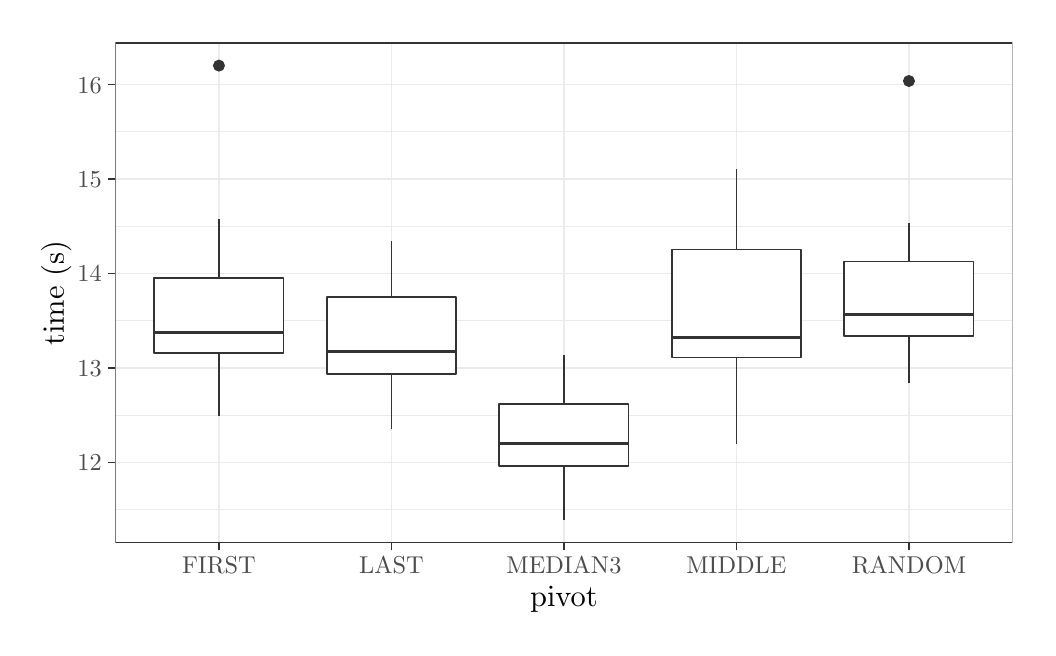
\begin{tikzpicture}[x=1pt,y=1pt]
\definecolor{fillColor}{RGB}{255,255,255}
\path[use as bounding box,fill=fillColor,fill opacity=0.00] (0,0) rectangle (361.35,216.81);
\begin{scope}
\path[clip] (  0.00,  0.00) rectangle (361.35,216.81);
\definecolor{drawColor}{RGB}{255,255,255}
\definecolor{fillColor}{RGB}{255,255,255}

\path[draw=drawColor,line width= 0.6pt,line join=round,line cap=round,fill=fillColor] (  0.00,  0.00) rectangle (361.35,216.81);
\end{scope}
\begin{scope}
\path[clip] ( 31.71, 30.69) rectangle (355.85,211.31);
\definecolor{fillColor}{RGB}{255,255,255}

\path[fill=fillColor] ( 31.71, 30.69) rectangle (355.85,211.31);
\definecolor{drawColor}{gray}{0.92}

\path[draw=drawColor,line width= 0.3pt,line join=round] ( 31.71, 42.62) --
	(355.85, 42.62);

\path[draw=drawColor,line width= 0.3pt,line join=round] ( 31.71, 76.76) --
	(355.85, 76.76);

\path[draw=drawColor,line width= 0.3pt,line join=round] ( 31.71,110.90) --
	(355.85,110.90);

\path[draw=drawColor,line width= 0.3pt,line join=round] ( 31.71,145.03) --
	(355.85,145.03);

\path[draw=drawColor,line width= 0.3pt,line join=round] ( 31.71,179.17) --
	(355.85,179.17);

\path[draw=drawColor,line width= 0.6pt,line join=round] ( 31.71, 59.69) --
	(355.85, 59.69);

\path[draw=drawColor,line width= 0.6pt,line join=round] ( 31.71, 93.83) --
	(355.85, 93.83);

\path[draw=drawColor,line width= 0.6pt,line join=round] ( 31.71,127.96) --
	(355.85,127.96);

\path[draw=drawColor,line width= 0.6pt,line join=round] ( 31.71,162.10) --
	(355.85,162.10);

\path[draw=drawColor,line width= 0.6pt,line join=round] ( 31.71,196.23) --
	(355.85,196.23);

\path[draw=drawColor,line width= 0.6pt,line join=round] ( 69.11, 30.69) --
	( 69.11,211.31);

\path[draw=drawColor,line width= 0.6pt,line join=round] (131.45, 30.69) --
	(131.45,211.31);

\path[draw=drawColor,line width= 0.6pt,line join=round] (193.78, 30.69) --
	(193.78,211.31);

\path[draw=drawColor,line width= 0.6pt,line join=round] (256.12, 30.69) --
	(256.12,211.31);

\path[draw=drawColor,line width= 0.6pt,line join=round] (318.45, 30.69) --
	(318.45,211.31);
\definecolor{drawColor}{gray}{0.20}
\definecolor{fillColor}{gray}{0.20}

\path[draw=drawColor,line width= 0.4pt,line join=round,line cap=round,fill=fillColor] ( 69.11,203.10) circle (  1.96);

\path[draw=drawColor,line width= 0.6pt,line join=round] ( 69.11,126.42) -- ( 69.11,147.56);

\path[draw=drawColor,line width= 0.6pt,line join=round] ( 69.11, 99.32) -- ( 69.11, 76.36);
\definecolor{fillColor}{RGB}{255,255,255}

\path[draw=drawColor,line width= 0.6pt,line join=round,line cap=round,fill=fillColor] ( 45.74,126.42) --
	( 45.74, 99.32) --
	( 92.49, 99.32) --
	( 92.49,126.42) --
	( 45.74,126.42) --
	cycle;

\path[draw=drawColor,line width= 1.1pt,line join=round] ( 45.74,106.79) -- ( 92.49,106.79);

\path[draw=drawColor,line width= 0.6pt,line join=round] (131.45,119.41) -- (131.45,139.70);

\path[draw=drawColor,line width= 0.6pt,line join=round] (131.45, 91.59) -- (131.45, 71.93);

\path[draw=drawColor,line width= 0.6pt,line join=round,line cap=round,fill=fillColor] (108.07,119.41) --
	(108.07, 91.59) --
	(154.82, 91.59) --
	(154.82,119.41) --
	(108.07,119.41) --
	cycle;

\path[draw=drawColor,line width= 1.1pt,line join=round] (108.07, 99.94) -- (154.82, 99.94);

\path[draw=drawColor,line width= 0.6pt,line join=round] (193.78, 80.84) -- (193.78, 98.51);

\path[draw=drawColor,line width= 0.6pt,line join=round] (193.78, 58.36) -- (193.78, 38.90);

\path[draw=drawColor,line width= 0.6pt,line join=round,line cap=round,fill=fillColor] (170.41, 80.84) --
	(170.41, 58.36) --
	(217.16, 58.36) --
	(217.16, 80.84) --
	(170.41, 80.84) --
	cycle;

\path[draw=drawColor,line width= 1.1pt,line join=round] (170.41, 66.56) -- (217.16, 66.56);

\path[draw=drawColor,line width= 0.6pt,line join=round] (256.12,136.69) -- (256.12,165.64);

\path[draw=drawColor,line width= 0.6pt,line join=round] (256.12, 97.57) -- (256.12, 66.31);

\path[draw=drawColor,line width= 0.6pt,line join=round,line cap=round,fill=fillColor] (232.74,136.69) --
	(232.74, 97.57) --
	(279.49, 97.57) --
	(279.49,136.69) --
	(232.74,136.69) --
	cycle;

\path[draw=drawColor,line width= 1.1pt,line join=round] (232.74,104.90) -- (279.49,104.90);
\definecolor{fillColor}{gray}{0.20}

\path[draw=drawColor,line width= 0.4pt,line join=round,line cap=round,fill=fillColor] (318.45,197.54) circle (  1.96);

\path[draw=drawColor,line width= 0.6pt,line join=round] (318.45,132.34) -- (318.45,146.38);

\path[draw=drawColor,line width= 0.6pt,line join=round] (318.45,105.37) -- (318.45, 88.31);
\definecolor{fillColor}{RGB}{255,255,255}

\path[draw=drawColor,line width= 0.6pt,line join=round,line cap=round,fill=fillColor] (295.07,132.34) --
	(295.07,105.37) --
	(341.82,105.37) --
	(341.82,132.34) --
	(295.07,132.34) --
	cycle;

\path[draw=drawColor,line width= 1.1pt,line join=round] (295.07,113.16) -- (341.82,113.16);

\path[draw=drawColor,line width= 0.6pt,line join=round,line cap=round] ( 31.71, 30.69) rectangle (355.85,211.31);
\end{scope}
\begin{scope}
\path[clip] (  0.00,  0.00) rectangle (361.35,216.81);
\definecolor{drawColor}{gray}{0.30}

\node[text=drawColor,anchor=base east,inner sep=0pt, outer sep=0pt, scale=  0.88] at ( 26.76, 56.66) {12};

\node[text=drawColor,anchor=base east,inner sep=0pt, outer sep=0pt, scale=  0.88] at ( 26.76, 90.80) {13};

\node[text=drawColor,anchor=base east,inner sep=0pt, outer sep=0pt, scale=  0.88] at ( 26.76,124.93) {14};

\node[text=drawColor,anchor=base east,inner sep=0pt, outer sep=0pt, scale=  0.88] at ( 26.76,159.07) {15};

\node[text=drawColor,anchor=base east,inner sep=0pt, outer sep=0pt, scale=  0.88] at ( 26.76,193.20) {16};
\end{scope}
\begin{scope}
\path[clip] (  0.00,  0.00) rectangle (361.35,216.81);
\definecolor{drawColor}{gray}{0.20}

\path[draw=drawColor,line width= 0.6pt,line join=round] ( 28.96, 59.69) --
	( 31.71, 59.69);

\path[draw=drawColor,line width= 0.6pt,line join=round] ( 28.96, 93.83) --
	( 31.71, 93.83);

\path[draw=drawColor,line width= 0.6pt,line join=round] ( 28.96,127.96) --
	( 31.71,127.96);

\path[draw=drawColor,line width= 0.6pt,line join=round] ( 28.96,162.10) --
	( 31.71,162.10);

\path[draw=drawColor,line width= 0.6pt,line join=round] ( 28.96,196.23) --
	( 31.71,196.23);
\end{scope}
\begin{scope}
\path[clip] (  0.00,  0.00) rectangle (361.35,216.81);
\definecolor{drawColor}{gray}{0.20}

\path[draw=drawColor,line width= 0.6pt,line join=round] ( 69.11, 27.94) --
	( 69.11, 30.69);

\path[draw=drawColor,line width= 0.6pt,line join=round] (131.45, 27.94) --
	(131.45, 30.69);

\path[draw=drawColor,line width= 0.6pt,line join=round] (193.78, 27.94) --
	(193.78, 30.69);

\path[draw=drawColor,line width= 0.6pt,line join=round] (256.12, 27.94) --
	(256.12, 30.69);

\path[draw=drawColor,line width= 0.6pt,line join=round] (318.45, 27.94) --
	(318.45, 30.69);
\end{scope}
\begin{scope}
\path[clip] (  0.00,  0.00) rectangle (361.35,216.81);
\definecolor{drawColor}{gray}{0.30}

\node[text=drawColor,anchor=base,inner sep=0pt, outer sep=0pt, scale=  0.88] at ( 69.11, 19.68) {FIRST};

\node[text=drawColor,anchor=base,inner sep=0pt, outer sep=0pt, scale=  0.88] at (131.45, 19.68) {LAST};

\node[text=drawColor,anchor=base,inner sep=0pt, outer sep=0pt, scale=  0.88] at (193.78, 19.68) {MEDIAN3};

\node[text=drawColor,anchor=base,inner sep=0pt, outer sep=0pt, scale=  0.88] at (256.12, 19.68) {MIDDLE};

\node[text=drawColor,anchor=base,inner sep=0pt, outer sep=0pt, scale=  0.88] at (318.45, 19.68) {RANDOM};
\end{scope}
\begin{scope}
\path[clip] (  0.00,  0.00) rectangle (361.35,216.81);
\definecolor{drawColor}{RGB}{0,0,0}

\node[text=drawColor,anchor=base,inner sep=0pt, outer sep=0pt, scale=  1.10] at (193.78,  7.64) {pivot};
\end{scope}
\begin{scope}
\path[clip] (  0.00,  0.00) rectangle (361.35,216.81);
\definecolor{drawColor}{RGB}{0,0,0}

\node[text=drawColor,rotate= 90.00,anchor=base,inner sep=0pt, outer sep=0pt, scale=  1.10] at ( 13.08,121.00) {time (s)};
\end{scope}
\end{tikzpicture}


La scelta del pivot diventa importante quando l'array in input risulta già
parzialmente o totalmente ordinato.
Il grafico sottostante riporta il tempo impiegato da \verb|quick_sort()| 
per scorrere un array già ordinato.

% Created by tikzDevice version 0.12.3.1 on 2022-05-01 19:43:58
% !TEX encoding = UTF-8 Unicode
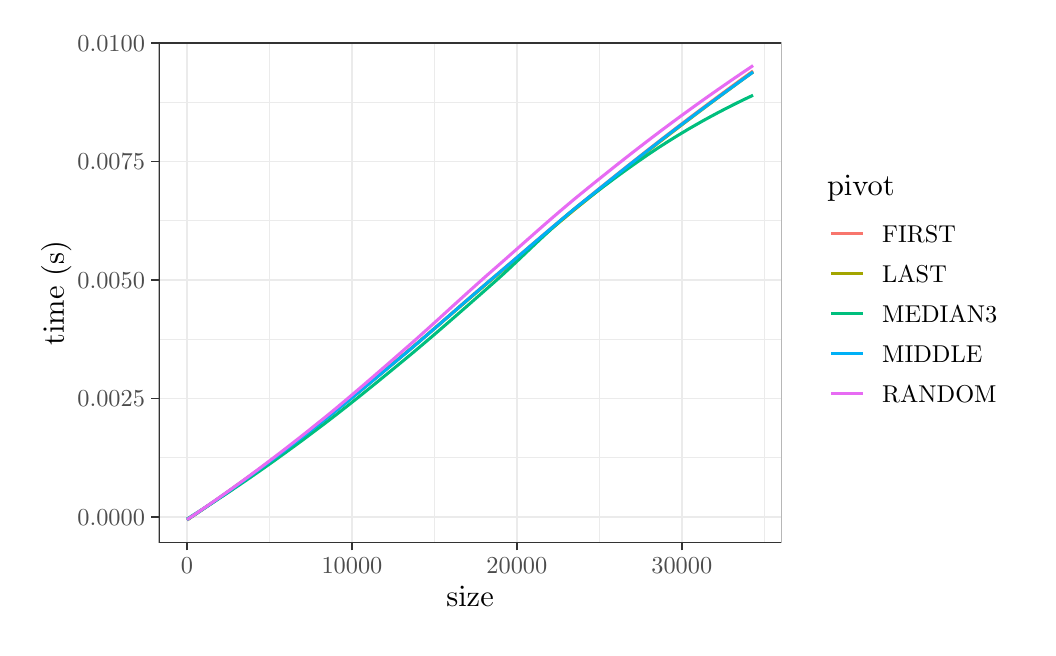
\begin{tikzpicture}[x=1pt,y=1pt]
\definecolor{fillColor}{RGB}{255,255,255}
\path[use as bounding box,fill=fillColor,fill opacity=0.00] (0,0) rectangle (361.35,216.81);
\begin{scope}
\path[clip] (  0.00,  0.00) rectangle (361.35,216.81);
\definecolor{drawColor}{RGB}{255,255,255}
\definecolor{fillColor}{RGB}{255,255,255}

\path[draw=drawColor,line width= 0.6pt,line join=round,line cap=round,fill=fillColor] (  0.00,  0.00) rectangle (361.35,216.81);
\end{scope}
\begin{scope}
\path[clip] ( 47.35, 30.69) rectangle (272.35,211.31);
\definecolor{fillColor}{RGB}{255,255,255}

\path[fill=fillColor] ( 47.35, 30.69) rectangle (272.35,211.31);
\definecolor{drawColor}{gray}{0.92}

\path[draw=drawColor,line width= 0.3pt,line join=round] ( 47.35, 61.46) --
	(272.35, 61.46);

\path[draw=drawColor,line width= 0.3pt,line join=round] ( 47.35,104.25) --
	(272.35,104.25);

\path[draw=drawColor,line width= 0.3pt,line join=round] ( 47.35,147.04) --
	(272.35,147.04);

\path[draw=drawColor,line width= 0.3pt,line join=round] ( 47.35,189.82) --
	(272.35,189.82);

\path[draw=drawColor,line width= 0.3pt,line join=round] ( 87.38, 30.69) --
	( 87.38,211.31);

\path[draw=drawColor,line width= 0.3pt,line join=round] (146.97, 30.69) --
	(146.97,211.31);

\path[draw=drawColor,line width= 0.3pt,line join=round] (206.57, 30.69) --
	(206.57,211.31);

\path[draw=drawColor,line width= 0.3pt,line join=round] (266.16, 30.69) --
	(266.16,211.31);

\path[draw=drawColor,line width= 0.6pt,line join=round] ( 47.35, 40.07) --
	(272.35, 40.07);

\path[draw=drawColor,line width= 0.6pt,line join=round] ( 47.35, 82.85) --
	(272.35, 82.85);

\path[draw=drawColor,line width= 0.6pt,line join=round] ( 47.35,125.64) --
	(272.35,125.64);

\path[draw=drawColor,line width= 0.6pt,line join=round] ( 47.35,168.43) --
	(272.35,168.43);

\path[draw=drawColor,line width= 0.6pt,line join=round] ( 47.35,211.22) --
	(272.35,211.22);

\path[draw=drawColor,line width= 0.6pt,line join=round] ( 57.58, 30.69) --
	( 57.58,211.31);

\path[draw=drawColor,line width= 0.6pt,line join=round] (117.18, 30.69) --
	(117.18,211.31);

\path[draw=drawColor,line width= 0.6pt,line join=round] (176.77, 30.69) --
	(176.77,211.31);

\path[draw=drawColor,line width= 0.6pt,line join=round] (236.37, 30.69) --
	(236.37,211.31);
\definecolor{drawColor}{RGB}{248,118,109}

\path[draw=drawColor,line width= 1.1pt,line join=round] ( 57.58, 38.99) --
	( 60.17, 40.72) --
	( 62.76, 42.46) --
	( 65.35, 44.23) --
	( 67.94, 46.01) --
	( 70.53, 47.81) --
	( 73.12, 49.63) --
	( 75.70, 51.46) --
	( 78.29, 53.31) --
	( 80.88, 55.18) --
	( 83.47, 57.06) --
	( 86.06, 58.96) --
	( 88.65, 60.88) --
	( 91.24, 62.82) --
	( 93.83, 64.77) --
	( 96.42, 66.74) --
	( 99.01, 68.72) --
	(101.60, 70.71) --
	(104.18, 72.72) --
	(106.77, 74.74) --
	(109.36, 76.79) --
	(111.95, 78.86) --
	(114.54, 80.95) --
	(117.13, 83.06) --
	(119.72, 85.18) --
	(122.31, 87.32) --
	(124.90, 89.47) --
	(127.49, 91.63) --
	(130.08, 93.79) --
	(132.67, 95.96) --
	(135.25, 98.14) --
	(137.84,100.31) --
	(140.43,102.51) --
	(143.02,104.72) --
	(145.61,106.96) --
	(148.20,109.20) --
	(150.79,111.46) --
	(153.38,113.71) --
	(155.97,115.97) --
	(158.56,118.22) --
	(161.15,120.46) --
	(163.74,122.68) --
	(166.32,124.89) --
	(168.91,127.08) --
	(171.50,129.28) --
	(174.09,131.48) --
	(176.68,133.70) --
	(179.27,135.91) --
	(181.86,138.13) --
	(184.45,140.34) --
	(187.04,142.55) --
	(189.63,144.74) --
	(192.22,146.92) --
	(194.81,149.08) --
	(197.39,151.22) --
	(199.98,153.34) --
	(202.57,155.44) --
	(205.16,157.53) --
	(207.75,159.62) --
	(210.34,161.70) --
	(212.93,163.78) --
	(215.52,165.84) --
	(218.11,167.90) --
	(220.70,169.94) --
	(223.29,171.98) --
	(225.88,174.00) --
	(228.46,176.01) --
	(231.05,178.01) --
	(233.64,180.00) --
	(236.23,181.97) --
	(238.82,183.94) --
	(241.41,185.89) --
	(244.00,187.83) --
	(246.59,189.77) --
	(249.18,191.69) --
	(251.77,193.60) --
	(254.36,195.51) --
	(256.94,197.40) --
	(259.53,199.28) --
	(262.12,201.16);
\definecolor{drawColor}{RGB}{163,165,0}

\path[draw=drawColor,line width= 1.1pt,line join=round] ( 57.58, 38.90) --
	( 60.17, 40.65) --
	( 62.76, 42.41) --
	( 65.35, 44.19) --
	( 67.94, 45.99) --
	( 70.53, 47.80) --
	( 73.12, 49.63) --
	( 75.70, 51.48) --
	( 78.29, 53.34) --
	( 80.88, 55.22) --
	( 83.47, 57.11) --
	( 86.06, 59.02) --
	( 88.65, 60.94) --
	( 91.24, 62.89) --
	( 93.83, 64.84) --
	( 96.42, 66.81) --
	( 99.01, 68.80) --
	(101.60, 70.79) --
	(104.18, 72.80) --
	(106.77, 74.82) --
	(109.36, 76.87) --
	(111.95, 78.93) --
	(114.54, 81.02) --
	(117.13, 83.12) --
	(119.72, 85.24) --
	(122.31, 87.37) --
	(124.90, 89.51) --
	(127.49, 91.66) --
	(130.08, 93.81) --
	(132.67, 95.97) --
	(135.25, 98.13) --
	(137.84,100.29) --
	(140.43,102.47) --
	(143.02,104.67) --
	(145.61,106.88) --
	(148.20,109.10) --
	(150.79,111.33) --
	(153.38,113.56) --
	(155.97,115.79) --
	(158.56,118.02) --
	(161.15,120.24) --
	(163.74,122.44) --
	(166.32,124.64) --
	(168.91,126.81) --
	(171.50,129.00) --
	(174.09,131.19) --
	(176.68,133.40) --
	(179.27,135.61) --
	(181.86,137.82) --
	(184.45,140.02) --
	(187.04,142.22) --
	(189.63,144.41) --
	(192.22,146.58) --
	(194.81,148.73) --
	(197.39,150.87) --
	(199.98,152.97) --
	(202.57,155.07) --
	(205.16,157.16) --
	(207.75,159.25) --
	(210.34,161.32) --
	(212.93,163.39) --
	(215.52,165.46) --
	(218.11,167.51) --
	(220.70,169.55) --
	(223.29,171.58) --
	(225.88,173.61) --
	(228.46,175.62) --
	(231.05,177.61) --
	(233.64,179.60) --
	(236.23,181.58) --
	(238.82,183.54) --
	(241.41,185.50) --
	(244.00,187.44) --
	(246.59,189.38) --
	(249.18,191.30) --
	(251.77,193.21) --
	(254.36,195.12) --
	(256.94,197.02) --
	(259.53,198.90) --
	(262.12,200.78);
\definecolor{drawColor}{RGB}{0,191,125}

\path[draw=drawColor,line width= 1.1pt,line join=round] ( 57.58, 39.26) --
	( 60.17, 40.89) --
	( 62.76, 42.53) --
	( 65.35, 44.19) --
	( 67.94, 45.87) --
	( 70.53, 47.57) --
	( 73.12, 49.29) --
	( 75.70, 51.04) --
	( 78.29, 52.79) --
	( 80.88, 54.57) --
	( 83.47, 56.36) --
	( 86.06, 58.18) --
	( 88.65, 60.01) --
	( 91.24, 61.87) --
	( 93.83, 63.74) --
	( 96.42, 65.63) --
	( 99.01, 67.53) --
	(101.60, 69.46) --
	(104.18, 71.39) --
	(106.77, 73.34) --
	(109.36, 75.32) --
	(111.95, 77.32) --
	(114.54, 79.35) --
	(117.13, 81.39) --
	(119.72, 83.45) --
	(122.31, 85.53) --
	(124.90, 87.62) --
	(127.49, 89.72) --
	(130.08, 91.84) --
	(132.67, 93.96) --
	(135.25, 96.09) --
	(137.84, 98.23) --
	(140.43,100.39) --
	(143.02,102.58) --
	(145.61,104.78) --
	(148.20,107.00) --
	(150.79,109.24) --
	(153.38,111.49) --
	(155.97,113.75) --
	(158.56,116.01) --
	(161.15,118.29) --
	(163.74,120.56) --
	(166.32,122.83) --
	(168.91,125.11) --
	(171.50,127.44) --
	(174.09,129.83) --
	(176.68,132.26) --
	(179.27,134.72) --
	(181.86,137.18) --
	(184.45,139.63) --
	(187.04,142.06) --
	(189.63,144.44) --
	(192.22,146.76) --
	(194.81,149.01) --
	(197.39,151.16) --
	(199.98,153.20) --
	(202.57,155.20) --
	(205.16,157.18) --
	(207.75,159.14) --
	(210.34,161.08) --
	(212.93,162.99) --
	(215.52,164.88) --
	(218.11,166.73) --
	(220.70,168.55) --
	(223.29,170.34) --
	(225.88,172.09) --
	(228.46,173.79) --
	(231.05,175.45) --
	(233.64,177.07) --
	(236.23,178.65) --
	(238.82,180.19) --
	(241.41,181.68) --
	(244.00,183.15) --
	(246.59,184.57) --
	(249.18,185.96) --
	(251.77,187.31) --
	(254.36,188.63) --
	(256.94,189.92) --
	(259.53,191.17) --
	(262.12,192.39);
\definecolor{drawColor}{RGB}{0,176,246}

\path[draw=drawColor,line width= 1.1pt,line join=round] ( 57.58, 38.98) --
	( 60.17, 40.71) --
	( 62.76, 42.46) --
	( 65.35, 44.23) --
	( 67.94, 46.01) --
	( 70.53, 47.82) --
	( 73.12, 49.64) --
	( 75.70, 51.47) --
	( 78.29, 53.32) --
	( 80.88, 55.19) --
	( 83.47, 57.07) --
	( 86.06, 58.97) --
	( 88.65, 60.89) --
	( 91.24, 62.83) --
	( 93.83, 64.78) --
	( 96.42, 66.74) --
	( 99.01, 68.72) --
	(101.60, 70.71) --
	(104.18, 72.72) --
	(106.77, 74.74) --
	(109.36, 76.78) --
	(111.95, 78.84) --
	(114.54, 80.93) --
	(117.13, 83.03) --
	(119.72, 85.15) --
	(122.31, 87.28) --
	(124.90, 89.42) --
	(127.49, 91.58) --
	(130.08, 93.74) --
	(132.67, 95.90) --
	(135.25, 98.07) --
	(137.84,100.24) --
	(140.43,102.43) --
	(143.02,104.65) --
	(145.61,106.88) --
	(148.20,109.12) --
	(150.79,111.38) --
	(153.38,113.63) --
	(155.97,115.89) --
	(158.56,118.14) --
	(161.15,120.38) --
	(163.74,122.61) --
	(166.32,124.82) --
	(168.91,127.01) --
	(171.50,129.21) --
	(174.09,131.42) --
	(176.68,133.63) --
	(179.27,135.85) --
	(181.86,138.07) --
	(184.45,140.29) --
	(187.04,142.49) --
	(189.63,144.69) --
	(192.22,146.87) --
	(194.81,149.03) --
	(197.39,151.16) --
	(199.98,153.27) --
	(202.57,155.36) --
	(205.16,157.45) --
	(207.75,159.53) --
	(210.34,161.61) --
	(212.93,163.67) --
	(215.52,165.73) --
	(218.11,167.78) --
	(220.70,169.81) --
	(223.29,171.84) --
	(225.88,173.85) --
	(228.46,175.85) --
	(231.05,177.84) --
	(233.64,179.81) --
	(236.23,181.77) --
	(238.82,183.72) --
	(241.41,185.66) --
	(244.00,187.59) --
	(246.59,189.50) --
	(249.18,191.41) --
	(251.77,193.31) --
	(254.36,195.19) --
	(256.94,197.06) --
	(259.53,198.93) --
	(262.12,200.78);
\definecolor{drawColor}{RGB}{231,107,243}

\path[draw=drawColor,line width= 1.1pt,line join=round] ( 57.58, 39.04) --
	( 60.17, 40.78) --
	( 62.76, 42.54) --
	( 65.35, 44.32) --
	( 67.94, 46.12) --
	( 70.53, 47.94) --
	( 73.12, 49.78) --
	( 75.70, 51.64) --
	( 78.29, 53.52) --
	( 80.88, 55.42) --
	( 83.47, 57.34) --
	( 86.06, 59.28) --
	( 88.65, 61.24) --
	( 91.24, 63.22) --
	( 93.83, 65.21) --
	( 96.42, 67.23) --
	( 99.01, 69.26) --
	(101.60, 71.31) --
	(104.18, 73.38) --
	(106.77, 75.46) --
	(109.36, 77.57) --
	(111.95, 79.71) --
	(114.54, 81.88) --
	(117.13, 84.07) --
	(119.72, 86.27) --
	(122.31, 88.50) --
	(124.90, 90.73) --
	(127.49, 92.98) --
	(130.08, 95.23) --
	(132.67, 97.49) --
	(135.25, 99.75) --
	(137.84,102.01) --
	(140.43,104.29) --
	(143.02,106.61) --
	(145.61,108.94) --
	(148.20,111.28) --
	(150.79,113.64) --
	(153.38,116.00) --
	(155.97,118.35) --
	(158.56,120.70) --
	(161.15,123.03) --
	(163.74,125.35) --
	(166.32,127.64) --
	(168.91,129.90) --
	(171.50,132.17) --
	(174.09,134.46) --
	(176.68,136.75) --
	(179.27,139.04) --
	(181.86,141.33) --
	(184.45,143.62) --
	(187.04,145.89) --
	(189.63,148.14) --
	(192.22,150.37) --
	(194.81,152.56) --
	(197.39,154.73) --
	(199.98,156.85) --
	(202.57,158.96) --
	(205.16,161.05) --
	(207.75,163.13) --
	(210.34,165.20) --
	(212.93,167.26) --
	(215.52,169.30) --
	(218.11,171.33) --
	(220.70,173.34) --
	(223.29,175.33) --
	(225.88,177.31) --
	(228.46,179.26) --
	(231.05,181.20) --
	(233.64,183.12) --
	(236.23,185.02) --
	(238.82,186.90) --
	(241.41,188.77) --
	(244.00,190.62) --
	(246.59,192.45) --
	(249.18,194.26) --
	(251.77,196.06) --
	(254.36,197.85) --
	(256.94,199.61) --
	(259.53,201.36) --
	(262.12,203.10);
\definecolor{drawColor}{gray}{0.20}

\path[draw=drawColor,line width= 0.6pt,line join=round,line cap=round] ( 47.35, 30.69) rectangle (272.35,211.31);
\end{scope}
\begin{scope}
\path[clip] (  0.00,  0.00) rectangle (361.35,216.81);
\definecolor{drawColor}{gray}{0.30}

\node[text=drawColor,anchor=base east,inner sep=0pt, outer sep=0pt, scale=  0.88] at ( 42.40, 37.04) {0.0000};

\node[text=drawColor,anchor=base east,inner sep=0pt, outer sep=0pt, scale=  0.88] at ( 42.40, 79.82) {0.0025};

\node[text=drawColor,anchor=base east,inner sep=0pt, outer sep=0pt, scale=  0.88] at ( 42.40,122.61) {0.0050};

\node[text=drawColor,anchor=base east,inner sep=0pt, outer sep=0pt, scale=  0.88] at ( 42.40,165.40) {0.0075};

\node[text=drawColor,anchor=base east,inner sep=0pt, outer sep=0pt, scale=  0.88] at ( 42.40,208.19) {0.0100};
\end{scope}
\begin{scope}
\path[clip] (  0.00,  0.00) rectangle (361.35,216.81);
\definecolor{drawColor}{gray}{0.20}

\path[draw=drawColor,line width= 0.6pt,line join=round] ( 44.60, 40.07) --
	( 47.35, 40.07);

\path[draw=drawColor,line width= 0.6pt,line join=round] ( 44.60, 82.85) --
	( 47.35, 82.85);

\path[draw=drawColor,line width= 0.6pt,line join=round] ( 44.60,125.64) --
	( 47.35,125.64);

\path[draw=drawColor,line width= 0.6pt,line join=round] ( 44.60,168.43) --
	( 47.35,168.43);

\path[draw=drawColor,line width= 0.6pt,line join=round] ( 44.60,211.22) --
	( 47.35,211.22);
\end{scope}
\begin{scope}
\path[clip] (  0.00,  0.00) rectangle (361.35,216.81);
\definecolor{drawColor}{gray}{0.20}

\path[draw=drawColor,line width= 0.6pt,line join=round] ( 57.58, 27.94) --
	( 57.58, 30.69);

\path[draw=drawColor,line width= 0.6pt,line join=round] (117.18, 27.94) --
	(117.18, 30.69);

\path[draw=drawColor,line width= 0.6pt,line join=round] (176.77, 27.94) --
	(176.77, 30.69);

\path[draw=drawColor,line width= 0.6pt,line join=round] (236.37, 27.94) --
	(236.37, 30.69);
\end{scope}
\begin{scope}
\path[clip] (  0.00,  0.00) rectangle (361.35,216.81);
\definecolor{drawColor}{gray}{0.30}

\node[text=drawColor,anchor=base,inner sep=0pt, outer sep=0pt, scale=  0.88] at ( 57.58, 19.68) {0};

\node[text=drawColor,anchor=base,inner sep=0pt, outer sep=0pt, scale=  0.88] at (117.18, 19.68) {10000};

\node[text=drawColor,anchor=base,inner sep=0pt, outer sep=0pt, scale=  0.88] at (176.77, 19.68) {20000};

\node[text=drawColor,anchor=base,inner sep=0pt, outer sep=0pt, scale=  0.88] at (236.37, 19.68) {30000};
\end{scope}
\begin{scope}
\path[clip] (  0.00,  0.00) rectangle (361.35,216.81);
\definecolor{drawColor}{RGB}{0,0,0}

\node[text=drawColor,anchor=base,inner sep=0pt, outer sep=0pt, scale=  1.10] at (159.85,  7.64) {size};
\end{scope}
\begin{scope}
\path[clip] (  0.00,  0.00) rectangle (361.35,216.81);
\definecolor{drawColor}{RGB}{0,0,0}

\node[text=drawColor,rotate= 90.00,anchor=base,inner sep=0pt, outer sep=0pt, scale=  1.10] at ( 13.08,121.00) {time (s)};
\end{scope}
\begin{scope}
\path[clip] (  0.00,  0.00) rectangle (361.35,216.81);
\definecolor{fillColor}{RGB}{255,255,255}

\path[fill=fillColor] (283.35, 71.76) rectangle (355.85,170.24);
\end{scope}
\begin{scope}
\path[clip] (  0.00,  0.00) rectangle (361.35,216.81);
\definecolor{drawColor}{RGB}{0,0,0}

\node[text=drawColor,anchor=base west,inner sep=0pt, outer sep=0pt, scale=  1.10] at (288.85,156.09) {pivot};
\end{scope}
\begin{scope}
\path[clip] (  0.00,  0.00) rectangle (361.35,216.81);
\definecolor{fillColor}{RGB}{255,255,255}

\path[fill=fillColor] (288.85,135.07) rectangle (303.30,149.53);
\end{scope}
\begin{scope}
\path[clip] (  0.00,  0.00) rectangle (361.35,216.81);
\definecolor{drawColor}{RGB}{248,118,109}

\path[draw=drawColor,line width= 1.1pt,line join=round] (290.30,142.30) -- (301.86,142.30);
\end{scope}
\begin{scope}
\path[clip] (  0.00,  0.00) rectangle (361.35,216.81);
\definecolor{fillColor}{RGB}{255,255,255}

\path[fill=fillColor] (288.85,120.62) rectangle (303.30,135.07);
\end{scope}
\begin{scope}
\path[clip] (  0.00,  0.00) rectangle (361.35,216.81);
\definecolor{drawColor}{RGB}{163,165,0}

\path[draw=drawColor,line width= 1.1pt,line join=round] (290.30,127.84) -- (301.86,127.84);
\end{scope}
\begin{scope}
\path[clip] (  0.00,  0.00) rectangle (361.35,216.81);
\definecolor{fillColor}{RGB}{255,255,255}

\path[fill=fillColor] (288.85,106.16) rectangle (303.30,120.62);
\end{scope}
\begin{scope}
\path[clip] (  0.00,  0.00) rectangle (361.35,216.81);
\definecolor{drawColor}{RGB}{0,191,125}

\path[draw=drawColor,line width= 1.1pt,line join=round] (290.30,113.39) -- (301.86,113.39);
\end{scope}
\begin{scope}
\path[clip] (  0.00,  0.00) rectangle (361.35,216.81);
\definecolor{fillColor}{RGB}{255,255,255}

\path[fill=fillColor] (288.85, 91.71) rectangle (303.30,106.16);
\end{scope}
\begin{scope}
\path[clip] (  0.00,  0.00) rectangle (361.35,216.81);
\definecolor{drawColor}{RGB}{0,176,246}

\path[draw=drawColor,line width= 1.1pt,line join=round] (290.30, 98.94) -- (301.86, 98.94);
\end{scope}
\begin{scope}
\path[clip] (  0.00,  0.00) rectangle (361.35,216.81);
\definecolor{fillColor}{RGB}{255,255,255}

\path[fill=fillColor] (288.85, 77.26) rectangle (303.30, 91.71);
\end{scope}
\begin{scope}
\path[clip] (  0.00,  0.00) rectangle (361.35,216.81);
\definecolor{drawColor}{RGB}{231,107,243}

\path[draw=drawColor,line width= 1.1pt,line join=round] (290.30, 84.48) -- (301.86, 84.48);
\end{scope}
\begin{scope}
\path[clip] (  0.00,  0.00) rectangle (361.35,216.81);
\definecolor{drawColor}{RGB}{0,0,0}

\node[text=drawColor,anchor=base west,inner sep=0pt, outer sep=0pt, scale=  0.88] at (308.80,139.27) {FIRST};
\end{scope}
\begin{scope}
\path[clip] (  0.00,  0.00) rectangle (361.35,216.81);
\definecolor{drawColor}{RGB}{0,0,0}

\node[text=drawColor,anchor=base west,inner sep=0pt, outer sep=0pt, scale=  0.88] at (308.80,124.81) {LAST};
\end{scope}
\begin{scope}
\path[clip] (  0.00,  0.00) rectangle (361.35,216.81);
\definecolor{drawColor}{RGB}{0,0,0}

\node[text=drawColor,anchor=base west,inner sep=0pt, outer sep=0pt, scale=  0.88] at (308.80,110.36) {MEDIAN3};
\end{scope}
\begin{scope}
\path[clip] (  0.00,  0.00) rectangle (361.35,216.81);
\definecolor{drawColor}{RGB}{0,0,0}

\node[text=drawColor,anchor=base west,inner sep=0pt, outer sep=0pt, scale=  0.88] at (308.80, 95.91) {MIDDLE};
\end{scope}
\begin{scope}
\path[clip] (  0.00,  0.00) rectangle (361.35,216.81);
\definecolor{drawColor}{RGB}{0,0,0}

\node[text=drawColor,anchor=base west,inner sep=0pt, outer sep=0pt, scale=  0.88] at (308.80, 81.45) {RANDOM};
\end{scope}
\end{tikzpicture}


Concentrandoci in particolare sui pivot \verb|median of 3|, \verb|random| e \verb|middle|, 
possiamo notare che anche tra questi 3 ve ne è uno preferibile rispetto agli altri (aggiungi qualcosa)
% Created by tikzDevice version 0.12.3.1 on 2022-05-05 16:00:32
% !TEX encoding = UTF-8 Unicode
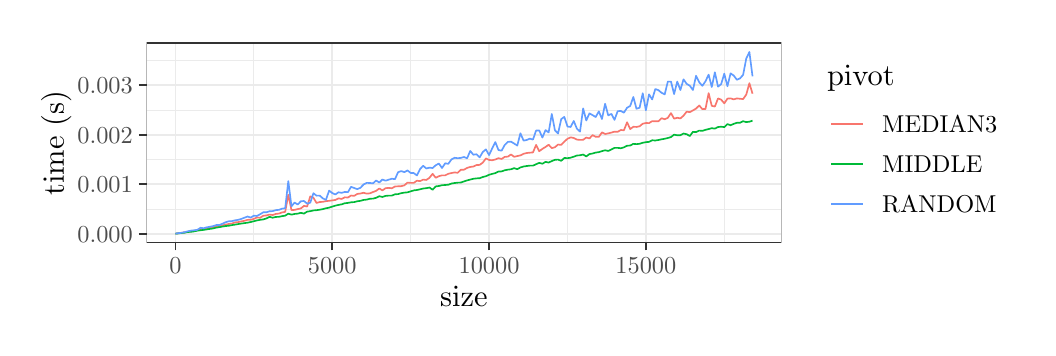
\begin{tikzpicture}[x=1pt,y=1pt]
\definecolor{fillColor}{RGB}{255,255,255}
\path[use as bounding box,fill=fillColor,fill opacity=0.00] (0,0) rectangle (361.35,108.41);
\begin{scope}
\path[clip] (  0.00,  0.00) rectangle (361.35,108.41);
\definecolor{drawColor}{RGB}{255,255,255}
\definecolor{fillColor}{RGB}{255,255,255}

\path[draw=drawColor,line width= 0.6pt,line join=round,line cap=round,fill=fillColor] (  0.00,  0.00) rectangle (361.35,108.41);
\end{scope}
\begin{scope}
\path[clip] ( 42.95, 30.69) rectangle (272.35,102.90);
\definecolor{fillColor}{RGB}{255,255,255}

\path[fill=fillColor] ( 42.95, 30.69) rectangle (272.35,102.91);
\definecolor{drawColor}{gray}{0.92}

\path[draw=drawColor,line width= 0.3pt,line join=round] ( 42.95, 42.91) --
	(272.35, 42.91);

\path[draw=drawColor,line width= 0.3pt,line join=round] ( 42.95, 60.78) --
	(272.35, 60.78);

\path[draw=drawColor,line width= 0.3pt,line join=round] ( 42.95, 78.66) --
	(272.35, 78.66);

\path[draw=drawColor,line width= 0.3pt,line join=round] ( 42.95, 96.53) --
	(272.35, 96.53);

\path[draw=drawColor,line width= 0.3pt,line join=round] ( 81.72, 30.69) --
	( 81.72,102.90);

\path[draw=drawColor,line width= 0.3pt,line join=round] (138.38, 30.69) --
	(138.38,102.90);

\path[draw=drawColor,line width= 0.3pt,line join=round] (195.05, 30.69) --
	(195.05,102.90);

\path[draw=drawColor,line width= 0.3pt,line join=round] (251.72, 30.69) --
	(251.72,102.90);

\path[draw=drawColor,line width= 0.6pt,line join=round] ( 42.95, 33.97) --
	(272.35, 33.97);

\path[draw=drawColor,line width= 0.6pt,line join=round] ( 42.95, 51.84) --
	(272.35, 51.84);

\path[draw=drawColor,line width= 0.6pt,line join=round] ( 42.95, 69.72) --
	(272.35, 69.72);

\path[draw=drawColor,line width= 0.6pt,line join=round] ( 42.95, 87.59) --
	(272.35, 87.59);

\path[draw=drawColor,line width= 0.6pt,line join=round] ( 53.38, 30.69) --
	( 53.38,102.90);

\path[draw=drawColor,line width= 0.6pt,line join=round] (110.05, 30.69) --
	(110.05,102.90);

\path[draw=drawColor,line width= 0.6pt,line join=round] (166.72, 30.69) --
	(166.72,102.90);

\path[draw=drawColor,line width= 0.6pt,line join=round] (223.39, 30.69) --
	(223.39,102.90);
\definecolor{drawColor}{RGB}{248,118,109}

\path[draw=drawColor,line width= 0.6pt,line join=round] ( 53.38, 33.97) --
	( 54.51, 34.13) --
	( 55.65, 34.29) --
	( 56.78, 34.45) --
	( 57.91, 34.61) --
	( 59.05, 34.81) --
	( 60.18, 35.02) --
	( 61.31, 35.24) --
	( 62.45, 35.47) --
	( 63.58, 35.70) --
	( 64.71, 35.92) --
	( 65.85, 36.15) --
	( 66.98, 36.36) --
	( 68.12, 36.56) --
	( 69.25, 36.81) --
	( 70.38, 36.95) --
	( 71.52, 37.26) --
	( 72.65, 37.47) --
	( 73.78, 37.63) --
	( 74.92, 38.06) --
	( 76.05, 38.15) --
	( 77.18, 38.42) --
	( 78.32, 38.62) --
	( 79.45, 38.97) --
	( 80.58, 38.99) --
	( 81.72, 39.31) --
	( 82.85, 39.83) --
	( 83.98, 39.72) --
	( 85.12, 40.44) --
	( 86.25, 40.56) --
	( 87.38, 40.87) --
	( 88.52, 40.71) --
	( 89.65, 41.10) --
	( 90.78, 41.24) --
	( 91.92, 41.65) --
	( 93.05, 41.85) --
	( 94.18, 48.02) --
	( 95.32, 42.49) --
	( 96.45, 42.57) --
	( 97.58, 42.85) --
	( 98.72, 43.10) --
	( 99.85, 44.01) --
	(100.98, 43.78) --
	(102.12, 47.48) --
	(103.25, 46.96) --
	(104.38, 45.07) --
	(105.52, 45.41) --
	(106.65, 45.48) --
	(107.78, 45.73) --
	(108.92, 45.84) --
	(110.05, 46.00) --
	(111.18, 46.16) --
	(112.32, 46.75) --
	(113.45, 46.52) --
	(114.58, 47.11) --
	(115.72, 47.03) --
	(116.85, 47.75) --
	(117.98, 47.64) --
	(119.12, 48.34) --
	(120.25, 48.48) --
	(121.38, 48.75) --
	(122.52, 48.43) --
	(123.65, 48.55) --
	(124.78, 49.02) --
	(125.92, 49.45) --
	(127.05, 50.31) --
	(128.18, 49.61) --
	(129.32, 50.41) --
	(130.45, 50.52) --
	(131.58, 50.38) --
	(132.72, 51.02) --
	(133.85, 51.09) --
	(134.98, 51.13) --
	(136.12, 51.45) --
	(137.25, 52.43) --
	(138.38, 52.33) --
	(139.52, 52.34) --
	(140.65, 53.11) --
	(141.78, 52.95) --
	(142.92, 53.51) --
	(144.05, 53.38) --
	(145.18, 54.17) --
	(146.32, 55.60) --
	(147.45, 54.17) --
	(148.59, 54.76) --
	(149.72, 55.04) --
	(150.85, 55.04) --
	(151.99, 55.61) --
	(153.12, 55.87) --
	(154.25, 56.10) --
	(155.39, 55.97) --
	(156.52, 57.06) --
	(157.65, 57.08) --
	(158.79, 57.74) --
	(159.92, 58.08) --
	(161.05, 58.24) --
	(162.19, 58.76) --
	(163.32, 58.83) --
	(164.45, 59.64) --
	(165.59, 61.17) --
	(166.72, 60.60) --
	(167.85, 60.51) --
	(168.99, 60.78) --
	(170.12, 61.26) --
	(171.25, 60.96) --
	(172.39, 61.71) --
	(173.52, 61.82) --
	(174.65, 62.59) --
	(175.79, 61.76) --
	(176.92, 62.01) --
	(178.05, 62.26) --
	(179.19, 62.84) --
	(180.32, 63.12) --
	(181.45, 63.23) --
	(182.59, 63.34) --
	(183.72, 66.04) --
	(184.85, 63.77) --
	(185.99, 64.61) --
	(187.12, 65.30) --
	(188.25, 66.11) --
	(189.39, 64.87) --
	(190.52, 65.21) --
	(191.65, 66.18) --
	(192.79, 66.05) --
	(193.92, 67.25) --
	(195.05, 68.25) --
	(196.19, 68.77) --
	(197.32, 68.56) --
	(198.45, 67.97) --
	(199.59, 67.86) --
	(200.72, 67.89) --
	(201.85, 68.72) --
	(202.99, 68.38) --
	(204.12, 69.59) --
	(205.25, 68.97) --
	(206.39, 68.95) --
	(207.52, 70.58) --
	(208.65, 69.99) --
	(209.79, 70.22) --
	(210.92, 70.49) --
	(212.05, 70.84) --
	(213.19, 70.77) --
	(214.32, 71.43) --
	(215.45, 71.33) --
	(216.59, 74.22) --
	(217.72, 71.76) --
	(218.85, 72.60) --
	(219.99, 72.54) --
	(221.12, 72.77) --
	(222.25, 73.70) --
	(223.39, 73.95) --
	(224.52, 73.92) --
	(225.66, 74.63) --
	(226.79, 74.60) --
	(227.92, 74.60) --
	(229.06, 75.69) --
	(230.19, 75.31) --
	(231.32, 75.83) --
	(232.46, 77.53) --
	(233.59, 75.53) --
	(234.72, 75.85) --
	(235.86, 75.63) --
	(236.99, 76.60) --
	(238.12, 78.07) --
	(239.26, 77.89) --
	(240.39, 78.51) --
	(241.52, 79.17) --
	(242.66, 80.30) --
	(243.79, 78.98) --
	(244.92, 79.03) --
	(246.06, 84.75) --
	(247.19, 80.17) --
	(248.32, 79.91) --
	(249.46, 82.84) --
	(250.59, 82.41) --
	(251.72, 81.07) --
	(252.86, 82.77) --
	(253.99, 82.87) --
	(255.12, 82.50) --
	(256.26, 82.86) --
	(257.39, 82.71) --
	(258.52, 82.62) --
	(259.66, 84.23) --
	(260.79, 88.34) --
	(261.92, 84.57);
\definecolor{drawColor}{RGB}{0,186,56}

\path[draw=drawColor,line width= 0.6pt,line join=round] ( 53.38, 33.97) --
	( 54.51, 34.08) --
	( 55.65, 34.22) --
	( 56.78, 34.34) --
	( 57.91, 34.58) --
	( 59.05, 34.65) --
	( 60.18, 34.81) --
	( 61.31, 35.06) --
	( 62.45, 35.20) --
	( 63.58, 35.34) --
	( 64.71, 35.52) --
	( 65.85, 35.70) --
	( 66.98, 35.86) --
	( 68.12, 36.15) --
	( 69.25, 36.33) --
	( 70.38, 36.54) --
	( 71.52, 36.74) --
	( 72.65, 36.83) --
	( 73.78, 37.06) --
	( 74.92, 37.24) --
	( 76.05, 37.44) --
	( 77.18, 37.63) --
	( 78.32, 37.78) --
	( 79.45, 37.95) --
	( 80.58, 38.17) --
	( 81.72, 38.47) --
	( 82.85, 38.76) --
	( 83.98, 38.97) --
	( 85.12, 39.12) --
	( 86.25, 39.47) --
	( 87.38, 40.06) --
	( 88.52, 39.74) --
	( 89.65, 40.01) --
	( 90.78, 40.06) --
	( 91.92, 40.30) --
	( 93.05, 40.49) --
	( 94.18, 41.19) --
	( 95.32, 40.85) --
	( 96.45, 41.10) --
	( 97.58, 41.21) --
	( 98.72, 41.51) --
	( 99.85, 41.23) --
	(100.98, 41.94) --
	(102.12, 42.10) --
	(103.25, 42.37) --
	(104.38, 42.46) --
	(105.52, 42.62) --
	(106.65, 42.85) --
	(107.78, 43.16) --
	(108.92, 43.37) --
	(110.05, 43.75) --
	(111.18, 44.10) --
	(112.32, 44.37) --
	(113.45, 44.57) --
	(114.58, 44.96) --
	(115.72, 45.09) --
	(116.85, 45.30) --
	(117.98, 45.39) --
	(119.12, 45.68) --
	(120.25, 45.84) --
	(121.38, 46.16) --
	(122.52, 46.28) --
	(123.65, 46.59) --
	(124.78, 46.64) --
	(125.92, 46.93) --
	(127.05, 47.50) --
	(128.18, 47.23) --
	(129.32, 47.61) --
	(130.45, 47.73) --
	(131.58, 47.73) --
	(132.72, 48.20) --
	(133.85, 48.27) --
	(134.98, 48.61) --
	(136.12, 48.80) --
	(137.25, 48.91) --
	(138.38, 49.25) --
	(139.52, 49.61) --
	(140.65, 49.75) --
	(141.78, 50.00) --
	(142.92, 50.29) --
	(144.05, 50.41) --
	(145.18, 50.65) --
	(146.32, 49.84) --
	(147.45, 51.06) --
	(148.59, 51.20) --
	(149.72, 51.49) --
	(150.85, 51.56) --
	(151.99, 51.66) --
	(153.12, 52.08) --
	(154.25, 52.27) --
	(155.39, 52.40) --
	(156.52, 52.45) --
	(157.65, 52.86) --
	(158.79, 53.22) --
	(159.92, 53.52) --
	(161.05, 53.81) --
	(162.19, 53.95) --
	(163.32, 54.02) --
	(164.45, 54.44) --
	(165.59, 54.74) --
	(166.72, 55.24) --
	(167.85, 55.58) --
	(168.99, 55.85) --
	(170.12, 56.42) --
	(171.25, 56.47) --
	(172.39, 56.88) --
	(173.52, 57.10) --
	(174.65, 57.24) --
	(175.79, 57.65) --
	(176.92, 57.29) --
	(178.05, 57.90) --
	(179.19, 58.24) --
	(180.32, 58.42) --
	(181.45, 58.55) --
	(182.59, 58.56) --
	(183.72, 59.06) --
	(184.85, 59.57) --
	(185.99, 59.24) --
	(187.12, 59.92) --
	(188.25, 59.67) --
	(189.39, 60.21) --
	(190.52, 60.66) --
	(191.65, 60.74) --
	(192.79, 60.30) --
	(193.92, 61.33) --
	(195.05, 61.25) --
	(196.19, 61.41) --
	(197.32, 61.78) --
	(198.45, 62.21) --
	(199.59, 62.30) --
	(200.72, 62.57) --
	(201.85, 61.89) --
	(202.99, 62.73) --
	(204.12, 62.94) --
	(205.25, 63.28) --
	(206.39, 63.44) --
	(207.52, 63.80) --
	(208.65, 64.11) --
	(209.79, 63.86) --
	(210.92, 64.39) --
	(212.05, 64.98) --
	(213.19, 64.98) --
	(214.32, 64.84) --
	(215.45, 65.16) --
	(216.59, 65.75) --
	(217.72, 65.82) --
	(218.85, 66.43) --
	(219.99, 66.32) --
	(221.12, 66.46) --
	(222.25, 66.82) --
	(223.39, 67.04) --
	(224.52, 67.14) --
	(225.66, 67.73) --
	(226.79, 67.63) --
	(227.92, 67.82) --
	(229.06, 68.07) --
	(230.19, 68.27) --
	(231.32, 68.54) --
	(232.46, 68.88) --
	(233.59, 69.77) --
	(234.72, 69.52) --
	(235.86, 69.54) --
	(236.99, 70.16) --
	(238.12, 69.91) --
	(239.26, 69.25) --
	(240.39, 70.77) --
	(241.52, 70.67) --
	(242.66, 71.22) --
	(243.79, 71.13) --
	(244.92, 71.49) --
	(246.06, 71.77) --
	(247.19, 72.10) --
	(248.32, 71.93) --
	(249.46, 72.51) --
	(250.59, 72.63) --
	(251.72, 72.47) --
	(252.86, 73.56) --
	(253.99, 73.15) --
	(255.12, 73.65) --
	(256.26, 74.03) --
	(257.39, 74.04) --
	(258.52, 74.60) --
	(259.66, 74.28) --
	(260.79, 74.44) --
	(261.92, 74.81);
\definecolor{drawColor}{RGB}{97,156,255}

\path[draw=drawColor,line width= 0.6pt,line join=round] ( 53.38, 33.99) --
	( 54.51, 34.17) --
	( 55.65, 34.29) --
	( 56.78, 34.54) --
	( 57.91, 34.84) --
	( 59.05, 35.08) --
	( 60.18, 35.20) --
	( 61.31, 35.36) --
	( 62.45, 36.10) --
	( 63.58, 35.93) --
	( 64.71, 36.27) --
	( 65.85, 36.47) --
	( 66.98, 36.70) --
	( 68.12, 37.08) --
	( 69.25, 37.11) --
	( 70.38, 37.56) --
	( 71.52, 38.10) --
	( 72.65, 38.44) --
	( 73.78, 38.51) --
	( 74.92, 38.79) --
	( 76.05, 38.97) --
	( 77.18, 39.30) --
	( 78.32, 39.74) --
	( 79.45, 40.17) --
	( 80.58, 39.78) --
	( 81.72, 40.46) --
	( 82.85, 40.37) --
	( 83.98, 40.99) --
	( 85.12, 41.69) --
	( 86.25, 41.71) --
	( 87.38, 42.07) --
	( 88.52, 42.12) --
	( 89.65, 42.48) --
	( 90.78, 42.58) --
	( 91.92, 43.01) --
	( 93.05, 43.16) --
	( 94.18, 52.97) --
	( 95.32, 43.85) --
	( 96.45, 45.23) --
	( 97.58, 44.50) --
	( 98.72, 45.69) --
	( 99.85, 45.78) --
	(100.98, 44.82) --
	(102.12, 45.18) --
	(103.25, 48.59) --
	(104.38, 47.70) --
	(105.52, 47.73) --
	(106.65, 46.73) --
	(107.78, 46.18) --
	(108.92, 49.52) --
	(110.05, 48.66) --
	(111.18, 48.14) --
	(112.32, 48.93) --
	(113.45, 48.73) --
	(114.58, 49.05) --
	(115.72, 48.97) --
	(116.85, 50.91) --
	(117.98, 50.47) --
	(119.12, 50.07) --
	(120.25, 50.56) --
	(121.38, 51.75) --
	(122.52, 52.33) --
	(123.65, 52.29) --
	(124.78, 52.16) --
	(125.92, 53.18) --
	(127.05, 52.45) --
	(128.18, 53.54) --
	(129.32, 53.11) --
	(130.45, 53.47) --
	(131.58, 53.83) --
	(132.72, 53.67) --
	(133.85, 56.19) --
	(134.98, 56.58) --
	(136.12, 56.20) --
	(137.25, 56.83) --
	(138.38, 55.92) --
	(139.52, 55.87) --
	(140.65, 55.01) --
	(141.78, 57.31) --
	(142.92, 58.49) --
	(144.05, 57.53) --
	(145.18, 57.83) --
	(146.32, 57.69) --
	(147.45, 58.69) --
	(148.59, 59.31) --
	(149.72, 57.71) --
	(150.85, 59.40) --
	(151.99, 59.21) --
	(153.12, 60.78) --
	(154.25, 61.39) --
	(155.39, 61.25) --
	(156.52, 61.35) --
	(157.65, 61.67) --
	(158.79, 61.21) --
	(159.92, 63.87) --
	(161.05, 62.50) --
	(162.19, 62.68) --
	(163.32, 61.55) --
	(164.45, 63.48) --
	(165.59, 64.43) --
	(166.72, 62.37) --
	(167.85, 64.78) --
	(168.99, 67.07) --
	(170.12, 64.18) --
	(171.25, 63.96) --
	(172.39, 66.04) --
	(173.52, 67.14) --
	(174.65, 67.22) --
	(175.79, 66.54) --
	(176.92, 65.80) --
	(178.05, 70.25) --
	(179.19, 67.61) --
	(180.32, 67.82) --
	(181.45, 68.31) --
	(182.59, 67.97) --
	(183.72, 71.22) --
	(184.85, 71.29) --
	(185.99, 68.70) --
	(187.12, 71.40) --
	(188.25, 70.54) --
	(189.39, 77.23) --
	(190.52, 71.33) --
	(191.65, 70.18) --
	(192.79, 75.37) --
	(193.92, 76.17) --
	(195.05, 72.69) --
	(196.19, 72.52) --
	(197.32, 74.70) --
	(198.45, 71.92) --
	(199.59, 70.86) --
	(200.72, 79.23) --
	(201.85, 74.88) --
	(202.99, 77.44) --
	(204.12, 76.81) --
	(205.25, 76.13) --
	(206.39, 78.17) --
	(207.52, 75.40) --
	(208.65, 80.91) --
	(209.79, 76.71) --
	(210.92, 77.26) --
	(212.05, 75.10) --
	(213.19, 78.23) --
	(214.32, 78.33) --
	(215.45, 77.69) --
	(216.59, 79.48) --
	(217.72, 80.12) --
	(218.85, 83.36) --
	(219.99, 79.12) --
	(221.12, 79.48) --
	(222.25, 84.71) --
	(223.39, 78.57) --
	(224.52, 84.32) --
	(225.66, 82.48) --
	(226.79, 86.23) --
	(227.92, 85.84) --
	(229.06, 84.86) --
	(230.19, 84.32) --
	(231.32, 88.93) --
	(232.46, 88.92) --
	(233.59, 84.41) --
	(234.72, 88.93) --
	(235.86, 85.89) --
	(236.99, 89.74) --
	(238.12, 88.11) --
	(239.26, 87.43) --
	(240.39, 85.88) --
	(241.52, 91.02) --
	(242.66, 88.67) --
	(243.79, 87.40) --
	(244.92, 89.02) --
	(246.06, 91.44) --
	(247.19, 86.97) --
	(248.32, 92.28) --
	(249.46, 87.09) --
	(250.59, 88.02) --
	(251.72, 91.79) --
	(252.86, 87.25) --
	(253.99, 91.90) --
	(255.12, 91.11) --
	(256.26, 89.59) --
	(257.39, 90.08) --
	(258.52, 91.36) --
	(259.66, 97.26) --
	(260.79, 99.62) --
	(261.92, 90.83);
\definecolor{drawColor}{gray}{0.20}

\path[draw=drawColor,line width= 0.6pt,line join=round,line cap=round] ( 42.95, 30.69) rectangle (272.35,102.91);
\end{scope}
\begin{scope}
\path[clip] (  0.00,  0.00) rectangle (361.35,108.41);
\definecolor{drawColor}{gray}{0.30}

\node[text=drawColor,anchor=base east,inner sep=0pt, outer sep=0pt, scale=  0.88] at ( 38.00, 30.94) {0.000};

\node[text=drawColor,anchor=base east,inner sep=0pt, outer sep=0pt, scale=  0.88] at ( 38.00, 48.81) {0.001};

\node[text=drawColor,anchor=base east,inner sep=0pt, outer sep=0pt, scale=  0.88] at ( 38.00, 66.69) {0.002};

\node[text=drawColor,anchor=base east,inner sep=0pt, outer sep=0pt, scale=  0.88] at ( 38.00, 84.56) {0.003};
\end{scope}
\begin{scope}
\path[clip] (  0.00,  0.00) rectangle (361.35,108.41);
\definecolor{drawColor}{gray}{0.20}

\path[draw=drawColor,line width= 0.6pt,line join=round] ( 40.20, 33.97) --
	( 42.95, 33.97);

\path[draw=drawColor,line width= 0.6pt,line join=round] ( 40.20, 51.84) --
	( 42.95, 51.84);

\path[draw=drawColor,line width= 0.6pt,line join=round] ( 40.20, 69.72) --
	( 42.95, 69.72);

\path[draw=drawColor,line width= 0.6pt,line join=round] ( 40.20, 87.59) --
	( 42.95, 87.59);
\end{scope}
\begin{scope}
\path[clip] (  0.00,  0.00) rectangle (361.35,108.41);
\definecolor{drawColor}{gray}{0.20}

\path[draw=drawColor,line width= 0.6pt,line join=round] ( 53.38, 27.94) --
	( 53.38, 30.69);

\path[draw=drawColor,line width= 0.6pt,line join=round] (110.05, 27.94) --
	(110.05, 30.69);

\path[draw=drawColor,line width= 0.6pt,line join=round] (166.72, 27.94) --
	(166.72, 30.69);

\path[draw=drawColor,line width= 0.6pt,line join=round] (223.39, 27.94) --
	(223.39, 30.69);
\end{scope}
\begin{scope}
\path[clip] (  0.00,  0.00) rectangle (361.35,108.41);
\definecolor{drawColor}{gray}{0.30}

\node[text=drawColor,anchor=base,inner sep=0pt, outer sep=0pt, scale=  0.88] at ( 53.38, 19.68) {0};

\node[text=drawColor,anchor=base,inner sep=0pt, outer sep=0pt, scale=  0.88] at (110.05, 19.68) {5000};

\node[text=drawColor,anchor=base,inner sep=0pt, outer sep=0pt, scale=  0.88] at (166.72, 19.68) {10000};

\node[text=drawColor,anchor=base,inner sep=0pt, outer sep=0pt, scale=  0.88] at (223.39, 19.68) {15000};
\end{scope}
\begin{scope}
\path[clip] (  0.00,  0.00) rectangle (361.35,108.41);
\definecolor{drawColor}{RGB}{0,0,0}

\node[text=drawColor,anchor=base,inner sep=0pt, outer sep=0pt, scale=  1.10] at (157.65,  7.64) {size};
\end{scope}
\begin{scope}
\path[clip] (  0.00,  0.00) rectangle (361.35,108.41);
\definecolor{drawColor}{RGB}{0,0,0}

\node[text=drawColor,rotate= 90.00,anchor=base,inner sep=0pt, outer sep=0pt, scale=  1.10] at ( 13.08, 66.80) {time (s)};
\end{scope}
\begin{scope}
\path[clip] (  0.00,  0.00) rectangle (361.35,108.41);
\definecolor{fillColor}{RGB}{255,255,255}

\path[fill=fillColor] (283.35, 32.01) rectangle (355.85,101.58);
\end{scope}
\begin{scope}
\path[clip] (  0.00,  0.00) rectangle (361.35,108.41);
\definecolor{drawColor}{RGB}{0,0,0}

\node[text=drawColor,anchor=base west,inner sep=0pt, outer sep=0pt, scale=  1.10] at (288.85, 87.44) {pivot};
\end{scope}
\begin{scope}
\path[clip] (  0.00,  0.00) rectangle (361.35,108.41);
\definecolor{fillColor}{RGB}{255,255,255}

\path[fill=fillColor] (288.85, 66.42) rectangle (303.30, 80.87);
\end{scope}
\begin{scope}
\path[clip] (  0.00,  0.00) rectangle (361.35,108.41);
\definecolor{drawColor}{RGB}{248,118,109}

\path[draw=drawColor,line width= 0.6pt,line join=round] (290.30, 73.64) -- (301.86, 73.64);
\end{scope}
\begin{scope}
\path[clip] (  0.00,  0.00) rectangle (361.35,108.41);
\definecolor{fillColor}{RGB}{255,255,255}

\path[fill=fillColor] (288.85, 51.96) rectangle (303.30, 66.42);
\end{scope}
\begin{scope}
\path[clip] (  0.00,  0.00) rectangle (361.35,108.41);
\definecolor{drawColor}{RGB}{0,186,56}

\path[draw=drawColor,line width= 0.6pt,line join=round] (290.30, 59.19) -- (301.86, 59.19);
\end{scope}
\begin{scope}
\path[clip] (  0.00,  0.00) rectangle (361.35,108.41);
\definecolor{fillColor}{RGB}{255,255,255}

\path[fill=fillColor] (288.85, 37.51) rectangle (303.30, 51.96);
\end{scope}
\begin{scope}
\path[clip] (  0.00,  0.00) rectangle (361.35,108.41);
\definecolor{drawColor}{RGB}{97,156,255}

\path[draw=drawColor,line width= 0.6pt,line join=round] (290.30, 44.73) -- (301.86, 44.73);
\end{scope}
\begin{scope}
\path[clip] (  0.00,  0.00) rectangle (361.35,108.41);
\definecolor{drawColor}{RGB}{0,0,0}

\node[text=drawColor,anchor=base west,inner sep=0pt, outer sep=0pt, scale=  0.88] at (308.80, 70.61) {MEDIAN3};
\end{scope}
\begin{scope}
\path[clip] (  0.00,  0.00) rectangle (361.35,108.41);
\definecolor{drawColor}{RGB}{0,0,0}

\node[text=drawColor,anchor=base west,inner sep=0pt, outer sep=0pt, scale=  0.88] at (308.80, 56.16) {MIDDLE};
\end{scope}
\begin{scope}
\path[clip] (  0.00,  0.00) rectangle (361.35,108.41);
\definecolor{drawColor}{RGB}{0,0,0}

\node[text=drawColor,anchor=base west,inner sep=0pt, outer sep=0pt, scale=  0.88] at (308.80, 41.70) {RANDOM};
\end{scope}
\end{tikzpicture}


\subsection{Fallback a Insertion Sort}
Quando il \verb|quick_sort()| lavora su un range sufficientemente piccolo, è più
efficiente utilizzare il \verb|insert_sort()|. Il range di cutoff è stato impostato a 8 elementi.

\section{Binary Insertion Sort}`
Essendo l'algoritmo di complessità $O(n^2)$, non ci aspettiamo che finisca in tempi
sensati l'ordinamento dei 20 milioni di records, facendo due calcoli sui nostri computer
dovrebbe metterci approssimativmaente 2 anni.


\chapter*{Esercizio 2}

\section{Skip List}

Bla bla bla insertion time decresce in maniera importante
% Created by tikzDevice version 0.12.3.1 on 2022-05-01 18:30:21
% !TEX encoding = UTF-8 Unicode
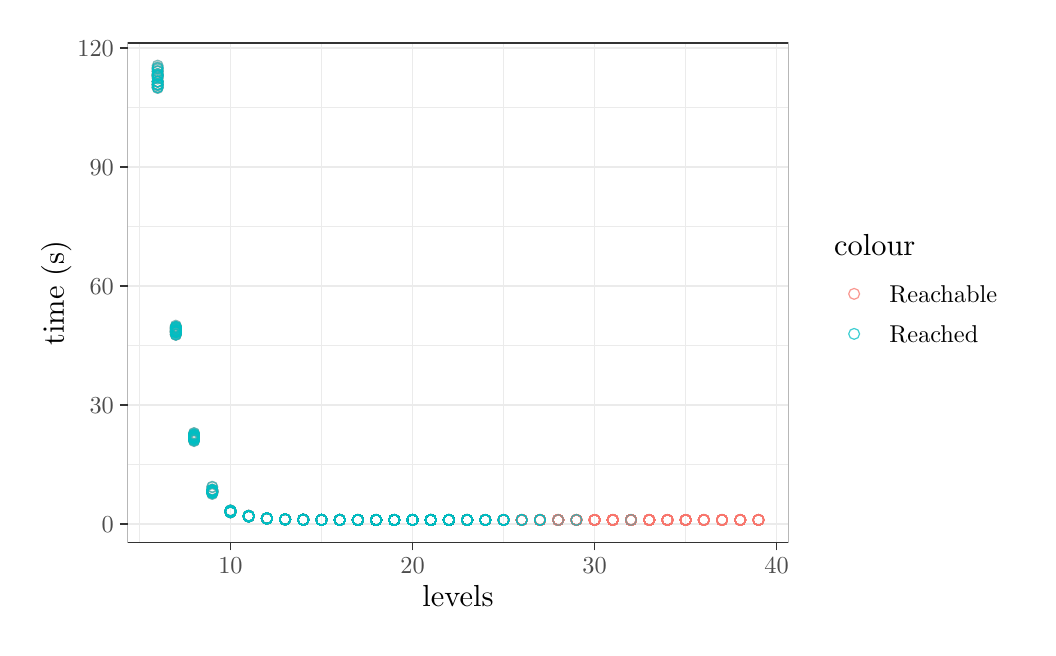
\begin{tikzpicture}[x=1pt,y=1pt]
\definecolor{fillColor}{RGB}{255,255,255}
\path[use as bounding box,fill=fillColor,fill opacity=0.00] (0,0) rectangle (361.35,216.81);
\begin{scope}
\path[clip] (  0.00,  0.00) rectangle (361.35,216.81);
\definecolor{drawColor}{RGB}{255,255,255}
\definecolor{fillColor}{RGB}{255,255,255}

\path[draw=drawColor,line width= 0.6pt,line join=round,line cap=round,fill=fillColor] (  0.00,  0.00) rectangle (361.35,216.81);
\end{scope}
\begin{scope}
\path[clip] ( 36.11, 30.69) rectangle (274.92,211.31);
\definecolor{fillColor}{RGB}{255,255,255}

\path[fill=fillColor] ( 36.11, 30.69) rectangle (274.92,211.31);
\definecolor{drawColor}{gray}{0.92}

\path[draw=drawColor,line width= 0.3pt,line join=round] ( 36.11, 59.01) --
	(274.92, 59.01);

\path[draw=drawColor,line width= 0.3pt,line join=round] ( 36.11,102.00) --
	(274.92,102.00);

\path[draw=drawColor,line width= 0.3pt,line join=round] ( 36.11,145.00) --
	(274.92,145.00);

\path[draw=drawColor,line width= 0.3pt,line join=round] ( 36.11,187.99) --
	(274.92,187.99);

\path[draw=drawColor,line width= 0.3pt,line join=round] ( 40.39, 30.69) --
	( 40.39,211.31);

\path[draw=drawColor,line width= 0.3pt,line join=round] (106.17, 30.69) --
	(106.17,211.31);

\path[draw=drawColor,line width= 0.3pt,line join=round] (171.96, 30.69) --
	(171.96,211.31);

\path[draw=drawColor,line width= 0.3pt,line join=round] (237.75, 30.69) --
	(237.75,211.31);

\path[draw=drawColor,line width= 0.6pt,line join=round] ( 36.11, 37.51) --
	(274.92, 37.51);

\path[draw=drawColor,line width= 0.6pt,line join=round] ( 36.11, 80.50) --
	(274.92, 80.50);

\path[draw=drawColor,line width= 0.6pt,line join=round] ( 36.11,123.50) --
	(274.92,123.50);

\path[draw=drawColor,line width= 0.6pt,line join=round] ( 36.11,166.50) --
	(274.92,166.50);

\path[draw=drawColor,line width= 0.6pt,line join=round] ( 36.11,209.49) --
	(274.92,209.49);

\path[draw=drawColor,line width= 0.6pt,line join=round] ( 73.28, 30.69) --
	( 73.28,211.31);

\path[draw=drawColor,line width= 0.6pt,line join=round] (139.07, 30.69) --
	(139.07,211.31);

\path[draw=drawColor,line width= 0.6pt,line join=round] (204.85, 30.69) --
	(204.85,211.31);

\path[draw=drawColor,line width= 0.6pt,line join=round] (270.64, 30.69) --
	(270.64,211.31);
\definecolor{drawColor}{RGB}{248,118,109}

\path[draw=drawColor,draw opacity=0.50,line width= 0.4pt,line join=round,line cap=round] ( 73.28, 41.76) circle (  1.96);

\path[draw=drawColor,draw opacity=0.50,line width= 0.4pt,line join=round,line cap=round] ( 73.28, 42.14) circle (  1.96);

\path[draw=drawColor,draw opacity=0.50,line width= 0.4pt,line join=round,line cap=round] ( 73.28, 42.16) circle (  1.96);

\path[draw=drawColor,draw opacity=0.50,line width= 0.4pt,line join=round,line cap=round] ( 73.28, 41.89) circle (  1.96);

\path[draw=drawColor,draw opacity=0.50,line width= 0.4pt,line join=round,line cap=round] ( 73.28, 42.10) circle (  1.96);

\path[draw=drawColor,draw opacity=0.50,line width= 0.4pt,line join=round,line cap=round] ( 73.28, 41.89) circle (  1.96);

\path[draw=drawColor,draw opacity=0.50,line width= 0.4pt,line join=round,line cap=round] ( 73.28, 41.75) circle (  1.96);

\path[draw=drawColor,draw opacity=0.50,line width= 0.4pt,line join=round,line cap=round] ( 73.28, 41.85) circle (  1.96);

\path[draw=drawColor,draw opacity=0.50,line width= 0.4pt,line join=round,line cap=round] ( 73.28, 42.06) circle (  1.96);

\path[draw=drawColor,draw opacity=0.50,line width= 0.4pt,line join=round,line cap=round] ( 73.28, 42.19) circle (  1.96);

\path[draw=drawColor,draw opacity=0.50,line width= 0.4pt,line join=round,line cap=round] ( 73.28, 41.97) circle (  1.96);

\path[draw=drawColor,draw opacity=0.50,line width= 0.4pt,line join=round,line cap=round] ( 73.28, 42.19) circle (  1.96);

\path[draw=drawColor,draw opacity=0.50,line width= 0.4pt,line join=round,line cap=round] ( 73.28, 42.02) circle (  1.96);

\path[draw=drawColor,draw opacity=0.50,line width= 0.4pt,line join=round,line cap=round] ( 73.28, 41.93) circle (  1.96);

\path[draw=drawColor,draw opacity=0.50,line width= 0.4pt,line join=round,line cap=round] ( 73.28, 42.22) circle (  1.96);

\path[draw=drawColor,draw opacity=0.50,line width= 0.4pt,line join=round,line cap=round] ( 73.28, 42.00) circle (  1.96);

\path[draw=drawColor,draw opacity=0.50,line width= 0.4pt,line join=round,line cap=round] ( 73.28, 41.96) circle (  1.96);

\path[draw=drawColor,draw opacity=0.50,line width= 0.4pt,line join=round,line cap=round] ( 73.28, 42.08) circle (  1.96);

\path[draw=drawColor,draw opacity=0.50,line width= 0.4pt,line join=round,line cap=round] ( 73.28, 42.30) circle (  1.96);

\path[draw=drawColor,draw opacity=0.50,line width= 0.4pt,line join=round,line cap=round] ( 73.28, 41.83) circle (  1.96);

\path[draw=drawColor,draw opacity=0.50,line width= 0.4pt,line join=round,line cap=round] ( 73.28, 41.87) circle (  1.96);

\path[draw=drawColor,draw opacity=0.50,line width= 0.4pt,line join=round,line cap=round] ( 73.28, 41.89) circle (  1.96);

\path[draw=drawColor,draw opacity=0.50,line width= 0.4pt,line join=round,line cap=round] ( 73.28, 41.95) circle (  1.96);

\path[draw=drawColor,draw opacity=0.50,line width= 0.4pt,line join=round,line cap=round] ( 73.28, 41.92) circle (  1.96);

\path[draw=drawColor,draw opacity=0.50,line width= 0.4pt,line join=round,line cap=round] ( 73.28, 41.90) circle (  1.96);

\path[draw=drawColor,draw opacity=0.50,line width= 0.4pt,line join=round,line cap=round] ( 73.28, 42.10) circle (  1.96);

\path[draw=drawColor,draw opacity=0.50,line width= 0.4pt,line join=round,line cap=round] ( 73.28, 41.96) circle (  1.96);

\path[draw=drawColor,draw opacity=0.50,line width= 0.4pt,line join=round,line cap=round] ( 73.28, 42.08) circle (  1.96);

\path[draw=drawColor,draw opacity=0.50,line width= 0.4pt,line join=round,line cap=round] ( 73.28, 42.22) circle (  1.96);

\path[draw=drawColor,draw opacity=0.50,line width= 0.4pt,line join=round,line cap=round] ( 73.28, 41.90) circle (  1.96);

\path[draw=drawColor,draw opacity=0.50,line width= 0.4pt,line join=round,line cap=round] ( 73.28, 42.28) circle (  1.96);

\path[draw=drawColor,draw opacity=0.50,line width= 0.4pt,line join=round,line cap=round] ( 73.28, 42.11) circle (  1.96);

\path[draw=drawColor,draw opacity=0.50,line width= 0.4pt,line join=round,line cap=round] ( 73.28, 42.03) circle (  1.96);

\path[draw=drawColor,draw opacity=0.50,line width= 0.4pt,line join=round,line cap=round] ( 73.28, 42.18) circle (  1.96);

\path[draw=drawColor,draw opacity=0.50,line width= 0.4pt,line join=round,line cap=round] ( 79.86, 40.17) circle (  1.96);

\path[draw=drawColor,draw opacity=0.50,line width= 0.4pt,line join=round,line cap=round] ( 79.86, 40.28) circle (  1.96);

\path[draw=drawColor,draw opacity=0.50,line width= 0.4pt,line join=round,line cap=round] ( 79.86, 40.22) circle (  1.96);

\path[draw=drawColor,draw opacity=0.50,line width= 0.4pt,line join=round,line cap=round] ( 79.86, 40.33) circle (  1.96);

\path[draw=drawColor,draw opacity=0.50,line width= 0.4pt,line join=round,line cap=round] ( 79.86, 40.47) circle (  1.96);

\path[draw=drawColor,draw opacity=0.50,line width= 0.4pt,line join=round,line cap=round] ( 79.86, 40.19) circle (  1.96);

\path[draw=drawColor,draw opacity=0.50,line width= 0.4pt,line join=round,line cap=round] ( 79.86, 40.29) circle (  1.96);

\path[draw=drawColor,draw opacity=0.50,line width= 0.4pt,line join=round,line cap=round] ( 79.86, 40.33) circle (  1.96);

\path[draw=drawColor,draw opacity=0.50,line width= 0.4pt,line join=round,line cap=round] ( 79.86, 40.20) circle (  1.96);

\path[draw=drawColor,draw opacity=0.50,line width= 0.4pt,line join=round,line cap=round] ( 79.86, 40.39) circle (  1.96);

\path[draw=drawColor,draw opacity=0.50,line width= 0.4pt,line join=round,line cap=round] ( 79.86, 40.27) circle (  1.96);

\path[draw=drawColor,draw opacity=0.50,line width= 0.4pt,line join=round,line cap=round] ( 79.86, 40.38) circle (  1.96);

\path[draw=drawColor,draw opacity=0.50,line width= 0.4pt,line join=round,line cap=round] ( 79.86, 40.37) circle (  1.96);

\path[draw=drawColor,draw opacity=0.50,line width= 0.4pt,line join=round,line cap=round] ( 79.86, 40.27) circle (  1.96);

\path[draw=drawColor,draw opacity=0.50,line width= 0.4pt,line join=round,line cap=round] ( 79.86, 40.28) circle (  1.96);

\path[draw=drawColor,draw opacity=0.50,line width= 0.4pt,line join=round,line cap=round] ( 79.86, 40.42) circle (  1.96);

\path[draw=drawColor,draw opacity=0.50,line width= 0.4pt,line join=round,line cap=round] ( 79.86, 40.23) circle (  1.96);

\path[draw=drawColor,draw opacity=0.50,line width= 0.4pt,line join=round,line cap=round] ( 79.86, 40.37) circle (  1.96);

\path[draw=drawColor,draw opacity=0.50,line width= 0.4pt,line join=round,line cap=round] ( 79.86, 40.29) circle (  1.96);

\path[draw=drawColor,draw opacity=0.50,line width= 0.4pt,line join=round,line cap=round] ( 79.86, 40.34) circle (  1.96);

\path[draw=drawColor,draw opacity=0.50,line width= 0.4pt,line join=round,line cap=round] ( 79.86, 40.29) circle (  1.96);

\path[draw=drawColor,draw opacity=0.50,line width= 0.4pt,line join=round,line cap=round] ( 79.86, 40.30) circle (  1.96);

\path[draw=drawColor,draw opacity=0.50,line width= 0.4pt,line join=round,line cap=round] ( 79.86, 40.18) circle (  1.96);

\path[draw=drawColor,draw opacity=0.50,line width= 0.4pt,line join=round,line cap=round] ( 79.86, 40.37) circle (  1.96);

\path[draw=drawColor,draw opacity=0.50,line width= 0.4pt,line join=round,line cap=round] ( 79.86, 40.21) circle (  1.96);

\path[draw=drawColor,draw opacity=0.50,line width= 0.4pt,line join=round,line cap=round] ( 79.86, 40.36) circle (  1.96);

\path[draw=drawColor,draw opacity=0.50,line width= 0.4pt,line join=round,line cap=round] ( 79.86, 40.30) circle (  1.96);

\path[draw=drawColor,draw opacity=0.50,line width= 0.4pt,line join=round,line cap=round] ( 79.86, 40.35) circle (  1.96);

\path[draw=drawColor,draw opacity=0.50,line width= 0.4pt,line join=round,line cap=round] ( 79.86, 40.33) circle (  1.96);

\path[draw=drawColor,draw opacity=0.50,line width= 0.4pt,line join=round,line cap=round] ( 79.86, 40.22) circle (  1.96);

\path[draw=drawColor,draw opacity=0.50,line width= 0.4pt,line join=round,line cap=round] ( 79.86, 40.37) circle (  1.96);

\path[draw=drawColor,draw opacity=0.50,line width= 0.4pt,line join=round,line cap=round] ( 79.86, 40.29) circle (  1.96);

\path[draw=drawColor,draw opacity=0.50,line width= 0.4pt,line join=round,line cap=round] ( 79.86, 40.34) circle (  1.96);

\path[draw=drawColor,draw opacity=0.50,line width= 0.4pt,line join=round,line cap=round] ( 86.44, 39.46) circle (  1.96);

\path[draw=drawColor,draw opacity=0.50,line width= 0.4pt,line join=round,line cap=round] ( 86.44, 39.51) circle (  1.96);

\path[draw=drawColor,draw opacity=0.50,line width= 0.4pt,line join=round,line cap=round] ( 86.44, 39.49) circle (  1.96);

\path[draw=drawColor,draw opacity=0.50,line width= 0.4pt,line join=round,line cap=round] ( 86.44, 39.53) circle (  1.96);

\path[draw=drawColor,draw opacity=0.50,line width= 0.4pt,line join=round,line cap=round] ( 86.44, 39.43) circle (  1.96);

\path[draw=drawColor,draw opacity=0.50,line width= 0.4pt,line join=round,line cap=round] ( 86.44, 39.46) circle (  1.96);

\path[draw=drawColor,draw opacity=0.50,line width= 0.4pt,line join=round,line cap=round] ( 86.44, 39.45) circle (  1.96);

\path[draw=drawColor,draw opacity=0.50,line width= 0.4pt,line join=round,line cap=round] ( 86.44, 39.39) circle (  1.96);

\path[draw=drawColor,draw opacity=0.50,line width= 0.4pt,line join=round,line cap=round] ( 86.44, 39.47) circle (  1.96);

\path[draw=drawColor,draw opacity=0.50,line width= 0.4pt,line join=round,line cap=round] ( 86.44, 39.49) circle (  1.96);

\path[draw=drawColor,draw opacity=0.50,line width= 0.4pt,line join=round,line cap=round] ( 86.44, 39.53) circle (  1.96);

\path[draw=drawColor,draw opacity=0.50,line width= 0.4pt,line join=round,line cap=round] ( 86.44, 39.49) circle (  1.96);

\path[draw=drawColor,draw opacity=0.50,line width= 0.4pt,line join=round,line cap=round] ( 86.44, 39.48) circle (  1.96);

\path[draw=drawColor,draw opacity=0.50,line width= 0.4pt,line join=round,line cap=round] ( 86.44, 39.47) circle (  1.96);

\path[draw=drawColor,draw opacity=0.50,line width= 0.4pt,line join=round,line cap=round] ( 86.44, 39.42) circle (  1.96);

\path[draw=drawColor,draw opacity=0.50,line width= 0.4pt,line join=round,line cap=round] ( 86.44, 39.54) circle (  1.96);

\path[draw=drawColor,draw opacity=0.50,line width= 0.4pt,line join=round,line cap=round] ( 86.44, 39.49) circle (  1.96);

\path[draw=drawColor,draw opacity=0.50,line width= 0.4pt,line join=round,line cap=round] ( 86.44, 39.47) circle (  1.96);

\path[draw=drawColor,draw opacity=0.50,line width= 0.4pt,line join=round,line cap=round] ( 86.44, 39.49) circle (  1.96);

\path[draw=drawColor,draw opacity=0.50,line width= 0.4pt,line join=round,line cap=round] ( 86.44, 39.40) circle (  1.96);

\path[draw=drawColor,draw opacity=0.50,line width= 0.4pt,line join=round,line cap=round] ( 86.44, 39.38) circle (  1.96);

\path[draw=drawColor,draw opacity=0.50,line width= 0.4pt,line join=round,line cap=round] ( 86.44, 39.49) circle (  1.96);

\path[draw=drawColor,draw opacity=0.50,line width= 0.4pt,line join=round,line cap=round] ( 86.44, 39.40) circle (  1.96);

\path[draw=drawColor,draw opacity=0.50,line width= 0.4pt,line join=round,line cap=round] ( 86.44, 39.56) circle (  1.96);

\path[draw=drawColor,draw opacity=0.50,line width= 0.4pt,line join=round,line cap=round] ( 86.44, 39.51) circle (  1.96);

\path[draw=drawColor,draw opacity=0.50,line width= 0.4pt,line join=round,line cap=round] ( 86.44, 39.49) circle (  1.96);

\path[draw=drawColor,draw opacity=0.50,line width= 0.4pt,line join=round,line cap=round] ( 86.44, 39.53) circle (  1.96);

\path[draw=drawColor,draw opacity=0.50,line width= 0.4pt,line join=round,line cap=round] ( 86.44, 39.44) circle (  1.96);

\path[draw=drawColor,draw opacity=0.50,line width= 0.4pt,line join=round,line cap=round] ( 86.44, 39.50) circle (  1.96);

\path[draw=drawColor,draw opacity=0.50,line width= 0.4pt,line join=round,line cap=round] ( 86.44, 39.40) circle (  1.96);

\path[draw=drawColor,draw opacity=0.50,line width= 0.4pt,line join=round,line cap=round] ( 86.44, 39.46) circle (  1.96);

\path[draw=drawColor,draw opacity=0.50,line width= 0.4pt,line join=round,line cap=round] ( 86.44, 39.49) circle (  1.96);

\path[draw=drawColor,draw opacity=0.50,line width= 0.4pt,line join=round,line cap=round] ( 86.44, 39.47) circle (  1.96);

\path[draw=drawColor,draw opacity=0.50,line width= 0.4pt,line join=round,line cap=round] ( 93.02, 39.14) circle (  1.96);

\path[draw=drawColor,draw opacity=0.50,line width= 0.4pt,line join=round,line cap=round] ( 93.02, 39.12) circle (  1.96);

\path[draw=drawColor,draw opacity=0.50,line width= 0.4pt,line join=round,line cap=round] ( 93.02, 39.12) circle (  1.96);

\path[draw=drawColor,draw opacity=0.50,line width= 0.4pt,line join=round,line cap=round] ( 93.02, 39.15) circle (  1.96);

\path[draw=drawColor,draw opacity=0.50,line width= 0.4pt,line join=round,line cap=round] ( 93.02, 39.08) circle (  1.96);

\path[draw=drawColor,draw opacity=0.50,line width= 0.4pt,line join=round,line cap=round] ( 93.02, 39.15) circle (  1.96);

\path[draw=drawColor,draw opacity=0.50,line width= 0.4pt,line join=round,line cap=round] ( 93.02, 39.14) circle (  1.96);

\path[draw=drawColor,draw opacity=0.50,line width= 0.4pt,line join=round,line cap=round] ( 93.02, 39.12) circle (  1.96);

\path[draw=drawColor,draw opacity=0.50,line width= 0.4pt,line join=round,line cap=round] ( 93.02, 39.15) circle (  1.96);

\path[draw=drawColor,draw opacity=0.50,line width= 0.4pt,line join=round,line cap=round] ( 93.02, 39.09) circle (  1.96);

\path[draw=drawColor,draw opacity=0.50,line width= 0.4pt,line join=round,line cap=round] ( 93.02, 39.13) circle (  1.96);

\path[draw=drawColor,draw opacity=0.50,line width= 0.4pt,line join=round,line cap=round] ( 93.02, 39.16) circle (  1.96);

\path[draw=drawColor,draw opacity=0.50,line width= 0.4pt,line join=round,line cap=round] ( 93.02, 39.11) circle (  1.96);

\path[draw=drawColor,draw opacity=0.50,line width= 0.4pt,line join=round,line cap=round] ( 93.02, 39.19) circle (  1.96);

\path[draw=drawColor,draw opacity=0.50,line width= 0.4pt,line join=round,line cap=round] ( 93.02, 39.12) circle (  1.96);

\path[draw=drawColor,draw opacity=0.50,line width= 0.4pt,line join=round,line cap=round] ( 93.02, 39.14) circle (  1.96);

\path[draw=drawColor,draw opacity=0.50,line width= 0.4pt,line join=round,line cap=round] ( 93.02, 39.09) circle (  1.96);

\path[draw=drawColor,draw opacity=0.50,line width= 0.4pt,line join=round,line cap=round] ( 93.02, 39.12) circle (  1.96);

\path[draw=drawColor,draw opacity=0.50,line width= 0.4pt,line join=round,line cap=round] ( 93.02, 39.08) circle (  1.96);

\path[draw=drawColor,draw opacity=0.50,line width= 0.4pt,line join=round,line cap=round] ( 93.02, 39.17) circle (  1.96);

\path[draw=drawColor,draw opacity=0.50,line width= 0.4pt,line join=round,line cap=round] ( 93.02, 39.13) circle (  1.96);

\path[draw=drawColor,draw opacity=0.50,line width= 0.4pt,line join=round,line cap=round] ( 93.02, 39.12) circle (  1.96);

\path[draw=drawColor,draw opacity=0.50,line width= 0.4pt,line join=round,line cap=round] ( 93.02, 39.09) circle (  1.96);

\path[draw=drawColor,draw opacity=0.50,line width= 0.4pt,line join=round,line cap=round] ( 93.02, 39.09) circle (  1.96);

\path[draw=drawColor,draw opacity=0.50,line width= 0.4pt,line join=round,line cap=round] ( 93.02, 39.18) circle (  1.96);

\path[draw=drawColor,draw opacity=0.50,line width= 0.4pt,line join=round,line cap=round] ( 93.02, 39.12) circle (  1.96);

\path[draw=drawColor,draw opacity=0.50,line width= 0.4pt,line join=round,line cap=round] ( 93.02, 39.09) circle (  1.96);

\path[draw=drawColor,draw opacity=0.50,line width= 0.4pt,line join=round,line cap=round] ( 93.02, 39.15) circle (  1.96);

\path[draw=drawColor,draw opacity=0.50,line width= 0.4pt,line join=round,line cap=round] ( 93.02, 39.10) circle (  1.96);

\path[draw=drawColor,draw opacity=0.50,line width= 0.4pt,line join=round,line cap=round] ( 93.02, 39.13) circle (  1.96);

\path[draw=drawColor,draw opacity=0.50,line width= 0.4pt,line join=round,line cap=round] ( 93.02, 39.12) circle (  1.96);

\path[draw=drawColor,draw opacity=0.50,line width= 0.4pt,line join=round,line cap=round] ( 93.02, 39.12) circle (  1.96);

\path[draw=drawColor,draw opacity=0.50,line width= 0.4pt,line join=round,line cap=round] ( 93.02, 39.16) circle (  1.96);

\path[draw=drawColor,draw opacity=0.50,line width= 0.4pt,line join=round,line cap=round] ( 99.60, 39.00) circle (  1.96);

\path[draw=drawColor,draw opacity=0.50,line width= 0.4pt,line join=round,line cap=round] ( 99.60, 39.00) circle (  1.96);

\path[draw=drawColor,draw opacity=0.50,line width= 0.4pt,line join=round,line cap=round] ( 99.60, 39.00) circle (  1.96);

\path[draw=drawColor,draw opacity=0.50,line width= 0.4pt,line join=round,line cap=round] ( 99.60, 39.01) circle (  1.96);

\path[draw=drawColor,draw opacity=0.50,line width= 0.4pt,line join=round,line cap=round] ( 99.60, 38.98) circle (  1.96);

\path[draw=drawColor,draw opacity=0.50,line width= 0.4pt,line join=round,line cap=round] ( 99.60, 39.00) circle (  1.96);

\path[draw=drawColor,draw opacity=0.50,line width= 0.4pt,line join=round,line cap=round] ( 99.60, 39.00) circle (  1.96);

\path[draw=drawColor,draw opacity=0.50,line width= 0.4pt,line join=round,line cap=round] ( 99.60, 39.03) circle (  1.96);

\path[draw=drawColor,draw opacity=0.50,line width= 0.4pt,line join=round,line cap=round] ( 99.60, 39.00) circle (  1.96);

\path[draw=drawColor,draw opacity=0.50,line width= 0.4pt,line join=round,line cap=round] ( 99.60, 38.97) circle (  1.96);

\path[draw=drawColor,draw opacity=0.50,line width= 0.4pt,line join=round,line cap=round] ( 99.60, 39.03) circle (  1.96);

\path[draw=drawColor,draw opacity=0.50,line width= 0.4pt,line join=round,line cap=round] ( 99.60, 39.01) circle (  1.96);

\path[draw=drawColor,draw opacity=0.50,line width= 0.4pt,line join=round,line cap=round] ( 99.60, 38.99) circle (  1.96);

\path[draw=drawColor,draw opacity=0.50,line width= 0.4pt,line join=round,line cap=round] ( 99.60, 39.00) circle (  1.96);

\path[draw=drawColor,draw opacity=0.50,line width= 0.4pt,line join=round,line cap=round] ( 99.60, 38.98) circle (  1.96);

\path[draw=drawColor,draw opacity=0.50,line width= 0.4pt,line join=round,line cap=round] ( 99.60, 38.99) circle (  1.96);

\path[draw=drawColor,draw opacity=0.50,line width= 0.4pt,line join=round,line cap=round] ( 99.60, 39.04) circle (  1.96);

\path[draw=drawColor,draw opacity=0.50,line width= 0.4pt,line join=round,line cap=round] ( 99.60, 39.01) circle (  1.96);

\path[draw=drawColor,draw opacity=0.50,line width= 0.4pt,line join=round,line cap=round] ( 99.60, 38.97) circle (  1.96);

\path[draw=drawColor,draw opacity=0.50,line width= 0.4pt,line join=round,line cap=round] ( 99.60, 39.00) circle (  1.96);

\path[draw=drawColor,draw opacity=0.50,line width= 0.4pt,line join=round,line cap=round] ( 99.60, 38.97) circle (  1.96);

\path[draw=drawColor,draw opacity=0.50,line width= 0.4pt,line join=round,line cap=round] ( 99.60, 39.01) circle (  1.96);

\path[draw=drawColor,draw opacity=0.50,line width= 0.4pt,line join=round,line cap=round] ( 99.60, 39.01) circle (  1.96);

\path[draw=drawColor,draw opacity=0.50,line width= 0.4pt,line join=round,line cap=round] ( 99.60, 39.00) circle (  1.96);

\path[draw=drawColor,draw opacity=0.50,line width= 0.4pt,line join=round,line cap=round] ( 99.60, 38.98) circle (  1.96);

\path[draw=drawColor,draw opacity=0.50,line width= 0.4pt,line join=round,line cap=round] ( 99.60, 38.97) circle (  1.96);

\path[draw=drawColor,draw opacity=0.50,line width= 0.4pt,line join=round,line cap=round] ( 99.60, 39.02) circle (  1.96);

\path[draw=drawColor,draw opacity=0.50,line width= 0.4pt,line join=round,line cap=round] ( 99.60, 39.01) circle (  1.96);

\path[draw=drawColor,draw opacity=0.50,line width= 0.4pt,line join=round,line cap=round] ( 99.60, 38.98) circle (  1.96);

\path[draw=drawColor,draw opacity=0.50,line width= 0.4pt,line join=round,line cap=round] ( 99.60, 39.00) circle (  1.96);

\path[draw=drawColor,draw opacity=0.50,line width= 0.4pt,line join=round,line cap=round] ( 99.60, 38.97) circle (  1.96);

\path[draw=drawColor,draw opacity=0.50,line width= 0.4pt,line join=round,line cap=round] ( 99.60, 39.00) circle (  1.96);

\path[draw=drawColor,draw opacity=0.50,line width= 0.4pt,line join=round,line cap=round] ( 99.60, 39.00) circle (  1.96);

\path[draw=drawColor,draw opacity=0.50,line width= 0.4pt,line join=round,line cap=round] (106.17, 38.93) circle (  1.96);

\path[draw=drawColor,draw opacity=0.50,line width= 0.4pt,line join=round,line cap=round] (106.17, 38.93) circle (  1.96);

\path[draw=drawColor,draw opacity=0.50,line width= 0.4pt,line join=round,line cap=round] (106.17, 38.94) circle (  1.96);

\path[draw=drawColor,draw opacity=0.50,line width= 0.4pt,line join=round,line cap=round] (106.17, 38.94) circle (  1.96);

\path[draw=drawColor,draw opacity=0.50,line width= 0.4pt,line join=round,line cap=round] (106.17, 38.95) circle (  1.96);

\path[draw=drawColor,draw opacity=0.50,line width= 0.4pt,line join=round,line cap=round] (106.17, 38.94) circle (  1.96);

\path[draw=drawColor,draw opacity=0.50,line width= 0.4pt,line join=round,line cap=round] (106.17, 38.95) circle (  1.96);

\path[draw=drawColor,draw opacity=0.50,line width= 0.4pt,line join=round,line cap=round] (106.17, 38.96) circle (  1.96);

\path[draw=drawColor,draw opacity=0.50,line width= 0.4pt,line join=round,line cap=round] (106.17, 38.94) circle (  1.96);

\path[draw=drawColor,draw opacity=0.50,line width= 0.4pt,line join=round,line cap=round] (106.17, 38.95) circle (  1.96);

\path[draw=drawColor,draw opacity=0.50,line width= 0.4pt,line join=round,line cap=round] (106.17, 38.95) circle (  1.96);

\path[draw=drawColor,draw opacity=0.50,line width= 0.4pt,line join=round,line cap=round] (106.17, 38.94) circle (  1.96);

\path[draw=drawColor,draw opacity=0.50,line width= 0.4pt,line join=round,line cap=round] (106.17, 38.95) circle (  1.96);

\path[draw=drawColor,draw opacity=0.50,line width= 0.4pt,line join=round,line cap=round] (106.17, 38.97) circle (  1.96);

\path[draw=drawColor,draw opacity=0.50,line width= 0.4pt,line join=round,line cap=round] (106.17, 38.96) circle (  1.96);

\path[draw=drawColor,draw opacity=0.50,line width= 0.4pt,line join=round,line cap=round] (106.17, 38.95) circle (  1.96);

\path[draw=drawColor,draw opacity=0.50,line width= 0.4pt,line join=round,line cap=round] (106.17, 38.93) circle (  1.96);

\path[draw=drawColor,draw opacity=0.50,line width= 0.4pt,line join=round,line cap=round] (106.17, 38.96) circle (  1.96);

\path[draw=drawColor,draw opacity=0.50,line width= 0.4pt,line join=round,line cap=round] (106.17, 38.96) circle (  1.96);

\path[draw=drawColor,draw opacity=0.50,line width= 0.4pt,line join=round,line cap=round] (106.17, 38.95) circle (  1.96);

\path[draw=drawColor,draw opacity=0.50,line width= 0.4pt,line join=round,line cap=round] (106.17, 38.96) circle (  1.96);

\path[draw=drawColor,draw opacity=0.50,line width= 0.4pt,line join=round,line cap=round] (106.17, 38.95) circle (  1.96);

\path[draw=drawColor,draw opacity=0.50,line width= 0.4pt,line join=round,line cap=round] (106.17, 38.96) circle (  1.96);

\path[draw=drawColor,draw opacity=0.50,line width= 0.4pt,line join=round,line cap=round] (106.17, 38.94) circle (  1.96);

\path[draw=drawColor,draw opacity=0.50,line width= 0.4pt,line join=round,line cap=round] (106.17, 38.95) circle (  1.96);

\path[draw=drawColor,draw opacity=0.50,line width= 0.4pt,line join=round,line cap=round] (106.17, 38.95) circle (  1.96);

\path[draw=drawColor,draw opacity=0.50,line width= 0.4pt,line join=round,line cap=round] (106.17, 38.94) circle (  1.96);

\path[draw=drawColor,draw opacity=0.50,line width= 0.4pt,line join=round,line cap=round] (106.17, 38.96) circle (  1.96);

\path[draw=drawColor,draw opacity=0.50,line width= 0.4pt,line join=round,line cap=round] (106.17, 38.95) circle (  1.96);

\path[draw=drawColor,draw opacity=0.50,line width= 0.4pt,line join=round,line cap=round] (106.17, 38.94) circle (  1.96);

\path[draw=drawColor,draw opacity=0.50,line width= 0.4pt,line join=round,line cap=round] (106.17, 38.96) circle (  1.96);

\path[draw=drawColor,draw opacity=0.50,line width= 0.4pt,line join=round,line cap=round] (106.17, 38.96) circle (  1.96);

\path[draw=drawColor,draw opacity=0.50,line width= 0.4pt,line join=round,line cap=round] (106.17, 38.94) circle (  1.96);

\path[draw=drawColor,draw opacity=0.50,line width= 0.4pt,line join=round,line cap=round] (112.75, 38.93) circle (  1.96);

\path[draw=drawColor,draw opacity=0.50,line width= 0.4pt,line join=round,line cap=round] (112.75, 38.94) circle (  1.96);

\path[draw=drawColor,draw opacity=0.50,line width= 0.4pt,line join=round,line cap=round] (112.75, 38.94) circle (  1.96);

\path[draw=drawColor,draw opacity=0.50,line width= 0.4pt,line join=round,line cap=round] (112.75, 38.94) circle (  1.96);

\path[draw=drawColor,draw opacity=0.50,line width= 0.4pt,line join=round,line cap=round] (112.75, 38.92) circle (  1.96);

\path[draw=drawColor,draw opacity=0.50,line width= 0.4pt,line join=round,line cap=round] (112.75, 38.94) circle (  1.96);

\path[draw=drawColor,draw opacity=0.50,line width= 0.4pt,line join=round,line cap=round] (112.75, 38.95) circle (  1.96);

\path[draw=drawColor,draw opacity=0.50,line width= 0.4pt,line join=round,line cap=round] (112.75, 38.93) circle (  1.96);

\path[draw=drawColor,draw opacity=0.50,line width= 0.4pt,line join=round,line cap=round] (112.75, 38.93) circle (  1.96);

\path[draw=drawColor,draw opacity=0.50,line width= 0.4pt,line join=round,line cap=round] (112.75, 38.93) circle (  1.96);

\path[draw=drawColor,draw opacity=0.50,line width= 0.4pt,line join=round,line cap=round] (112.75, 38.94) circle (  1.96);

\path[draw=drawColor,draw opacity=0.50,line width= 0.4pt,line join=round,line cap=round] (112.75, 38.95) circle (  1.96);

\path[draw=drawColor,draw opacity=0.50,line width= 0.4pt,line join=round,line cap=round] (112.75, 38.94) circle (  1.96);

\path[draw=drawColor,draw opacity=0.50,line width= 0.4pt,line join=round,line cap=round] (112.75, 38.93) circle (  1.96);

\path[draw=drawColor,draw opacity=0.50,line width= 0.4pt,line join=round,line cap=round] (112.75, 38.94) circle (  1.96);

\path[draw=drawColor,draw opacity=0.50,line width= 0.4pt,line join=round,line cap=round] (112.75, 38.94) circle (  1.96);

\path[draw=drawColor,draw opacity=0.50,line width= 0.4pt,line join=round,line cap=round] (112.75, 38.94) circle (  1.96);

\path[draw=drawColor,draw opacity=0.50,line width= 0.4pt,line join=round,line cap=round] (112.75, 38.94) circle (  1.96);

\path[draw=drawColor,draw opacity=0.50,line width= 0.4pt,line join=round,line cap=round] (112.75, 38.94) circle (  1.96);

\path[draw=drawColor,draw opacity=0.50,line width= 0.4pt,line join=round,line cap=round] (112.75, 38.93) circle (  1.96);

\path[draw=drawColor,draw opacity=0.50,line width= 0.4pt,line join=round,line cap=round] (112.75, 38.94) circle (  1.96);

\path[draw=drawColor,draw opacity=0.50,line width= 0.4pt,line join=round,line cap=round] (112.75, 38.93) circle (  1.96);

\path[draw=drawColor,draw opacity=0.50,line width= 0.4pt,line join=round,line cap=round] (112.75, 38.93) circle (  1.96);

\path[draw=drawColor,draw opacity=0.50,line width= 0.4pt,line join=round,line cap=round] (112.75, 38.93) circle (  1.96);

\path[draw=drawColor,draw opacity=0.50,line width= 0.4pt,line join=round,line cap=round] (112.75, 38.95) circle (  1.96);

\path[draw=drawColor,draw opacity=0.50,line width= 0.4pt,line join=round,line cap=round] (112.75, 38.95) circle (  1.96);

\path[draw=drawColor,draw opacity=0.50,line width= 0.4pt,line join=round,line cap=round] (112.75, 38.92) circle (  1.96);

\path[draw=drawColor,draw opacity=0.50,line width= 0.4pt,line join=round,line cap=round] (112.75, 38.94) circle (  1.96);

\path[draw=drawColor,draw opacity=0.50,line width= 0.4pt,line join=round,line cap=round] (112.75, 38.92) circle (  1.96);

\path[draw=drawColor,draw opacity=0.50,line width= 0.4pt,line join=round,line cap=round] (112.75, 38.95) circle (  1.96);

\path[draw=drawColor,draw opacity=0.50,line width= 0.4pt,line join=round,line cap=round] (112.75, 38.95) circle (  1.96);

\path[draw=drawColor,draw opacity=0.50,line width= 0.4pt,line join=round,line cap=round] (112.75, 38.93) circle (  1.96);

\path[draw=drawColor,draw opacity=0.50,line width= 0.4pt,line join=round,line cap=round] (112.75, 38.93) circle (  1.96);

\path[draw=drawColor,draw opacity=0.50,line width= 0.4pt,line join=round,line cap=round] (119.33, 38.92) circle (  1.96);

\path[draw=drawColor,draw opacity=0.50,line width= 0.4pt,line join=round,line cap=round] (119.33, 38.94) circle (  1.96);

\path[draw=drawColor,draw opacity=0.50,line width= 0.4pt,line join=round,line cap=round] (119.33, 38.92) circle (  1.96);

\path[draw=drawColor,draw opacity=0.50,line width= 0.4pt,line join=round,line cap=round] (119.33, 38.93) circle (  1.96);

\path[draw=drawColor,draw opacity=0.50,line width= 0.4pt,line join=round,line cap=round] (119.33, 38.92) circle (  1.96);

\path[draw=drawColor,draw opacity=0.50,line width= 0.4pt,line join=round,line cap=round] (119.33, 38.93) circle (  1.96);

\path[draw=drawColor,draw opacity=0.50,line width= 0.4pt,line join=round,line cap=round] (119.33, 38.92) circle (  1.96);

\path[draw=drawColor,draw opacity=0.50,line width= 0.4pt,line join=round,line cap=round] (119.33, 38.93) circle (  1.96);

\path[draw=drawColor,draw opacity=0.50,line width= 0.4pt,line join=round,line cap=round] (119.33, 38.94) circle (  1.96);

\path[draw=drawColor,draw opacity=0.50,line width= 0.4pt,line join=round,line cap=round] (119.33, 38.93) circle (  1.96);

\path[draw=drawColor,draw opacity=0.50,line width= 0.4pt,line join=round,line cap=round] (119.33, 38.94) circle (  1.96);

\path[draw=drawColor,draw opacity=0.50,line width= 0.4pt,line join=round,line cap=round] (119.33, 38.93) circle (  1.96);

\path[draw=drawColor,draw opacity=0.50,line width= 0.4pt,line join=round,line cap=round] (119.33, 38.92) circle (  1.96);

\path[draw=drawColor,draw opacity=0.50,line width= 0.4pt,line join=round,line cap=round] (119.33, 38.93) circle (  1.96);

\path[draw=drawColor,draw opacity=0.50,line width= 0.4pt,line join=round,line cap=round] (119.33, 38.93) circle (  1.96);

\path[draw=drawColor,draw opacity=0.50,line width= 0.4pt,line join=round,line cap=round] (119.33, 38.93) circle (  1.96);

\path[draw=drawColor,draw opacity=0.50,line width= 0.4pt,line join=round,line cap=round] (119.33, 38.93) circle (  1.96);

\path[draw=drawColor,draw opacity=0.50,line width= 0.4pt,line join=round,line cap=round] (119.33, 38.94) circle (  1.96);

\path[draw=drawColor,draw opacity=0.50,line width= 0.4pt,line join=round,line cap=round] (119.33, 38.92) circle (  1.96);

\path[draw=drawColor,draw opacity=0.50,line width= 0.4pt,line join=round,line cap=round] (119.33, 38.92) circle (  1.96);

\path[draw=drawColor,draw opacity=0.50,line width= 0.4pt,line join=round,line cap=round] (119.33, 38.93) circle (  1.96);

\path[draw=drawColor,draw opacity=0.50,line width= 0.4pt,line join=round,line cap=round] (119.33, 38.93) circle (  1.96);

\path[draw=drawColor,draw opacity=0.50,line width= 0.4pt,line join=round,line cap=round] (119.33, 38.91) circle (  1.96);

\path[draw=drawColor,draw opacity=0.50,line width= 0.4pt,line join=round,line cap=round] (119.33, 38.93) circle (  1.96);

\path[draw=drawColor,draw opacity=0.50,line width= 0.4pt,line join=round,line cap=round] (119.33, 38.93) circle (  1.96);

\path[draw=drawColor,draw opacity=0.50,line width= 0.4pt,line join=round,line cap=round] (119.33, 38.92) circle (  1.96);

\path[draw=drawColor,draw opacity=0.50,line width= 0.4pt,line join=round,line cap=round] (119.33, 38.94) circle (  1.96);

\path[draw=drawColor,draw opacity=0.50,line width= 0.4pt,line join=round,line cap=round] (119.33, 38.93) circle (  1.96);

\path[draw=drawColor,draw opacity=0.50,line width= 0.4pt,line join=round,line cap=round] (119.33, 38.93) circle (  1.96);

\path[draw=drawColor,draw opacity=0.50,line width= 0.4pt,line join=round,line cap=round] (119.33, 38.93) circle (  1.96);

\path[draw=drawColor,draw opacity=0.50,line width= 0.4pt,line join=round,line cap=round] (119.33, 38.93) circle (  1.96);

\path[draw=drawColor,draw opacity=0.50,line width= 0.4pt,line join=round,line cap=round] (119.33, 38.92) circle (  1.96);

\path[draw=drawColor,draw opacity=0.50,line width= 0.4pt,line join=round,line cap=round] (119.33, 38.92) circle (  1.96);

\path[draw=drawColor,draw opacity=0.50,line width= 0.4pt,line join=round,line cap=round] (125.91, 38.94) circle (  1.96);

\path[draw=drawColor,draw opacity=0.50,line width= 0.4pt,line join=round,line cap=round] (125.91, 38.92) circle (  1.96);

\path[draw=drawColor,draw opacity=0.50,line width= 0.4pt,line join=round,line cap=round] (125.91, 38.92) circle (  1.96);

\path[draw=drawColor,draw opacity=0.50,line width= 0.4pt,line join=round,line cap=round] (125.91, 38.92) circle (  1.96);

\path[draw=drawColor,draw opacity=0.50,line width= 0.4pt,line join=round,line cap=round] (125.91, 38.92) circle (  1.96);

\path[draw=drawColor,draw opacity=0.50,line width= 0.4pt,line join=round,line cap=round] (125.91, 38.92) circle (  1.96);

\path[draw=drawColor,draw opacity=0.50,line width= 0.4pt,line join=round,line cap=round] (125.91, 38.93) circle (  1.96);

\path[draw=drawColor,draw opacity=0.50,line width= 0.4pt,line join=round,line cap=round] (125.91, 38.92) circle (  1.96);

\path[draw=drawColor,draw opacity=0.50,line width= 0.4pt,line join=round,line cap=round] (125.91, 38.92) circle (  1.96);

\path[draw=drawColor,draw opacity=0.50,line width= 0.4pt,line join=round,line cap=round] (125.91, 38.92) circle (  1.96);

\path[draw=drawColor,draw opacity=0.50,line width= 0.4pt,line join=round,line cap=round] (125.91, 38.92) circle (  1.96);

\path[draw=drawColor,draw opacity=0.50,line width= 0.4pt,line join=round,line cap=round] (125.91, 38.93) circle (  1.96);

\path[draw=drawColor,draw opacity=0.50,line width= 0.4pt,line join=round,line cap=round] (125.91, 38.93) circle (  1.96);

\path[draw=drawColor,draw opacity=0.50,line width= 0.4pt,line join=round,line cap=round] (125.91, 38.92) circle (  1.96);

\path[draw=drawColor,draw opacity=0.50,line width= 0.4pt,line join=round,line cap=round] (125.91, 38.91) circle (  1.96);

\path[draw=drawColor,draw opacity=0.50,line width= 0.4pt,line join=round,line cap=round] (125.91, 38.92) circle (  1.96);

\path[draw=drawColor,draw opacity=0.50,line width= 0.4pt,line join=round,line cap=round] (125.91, 38.92) circle (  1.96);

\path[draw=drawColor,draw opacity=0.50,line width= 0.4pt,line join=round,line cap=round] (125.91, 38.93) circle (  1.96);

\path[draw=drawColor,draw opacity=0.50,line width= 0.4pt,line join=round,line cap=round] (125.91, 38.92) circle (  1.96);

\path[draw=drawColor,draw opacity=0.50,line width= 0.4pt,line join=round,line cap=round] (125.91, 38.93) circle (  1.96);

\path[draw=drawColor,draw opacity=0.50,line width= 0.4pt,line join=round,line cap=round] (125.91, 38.92) circle (  1.96);

\path[draw=drawColor,draw opacity=0.50,line width= 0.4pt,line join=round,line cap=round] (125.91, 38.92) circle (  1.96);

\path[draw=drawColor,draw opacity=0.50,line width= 0.4pt,line join=round,line cap=round] (125.91, 38.93) circle (  1.96);

\path[draw=drawColor,draw opacity=0.50,line width= 0.4pt,line join=round,line cap=round] (125.91, 38.92) circle (  1.96);

\path[draw=drawColor,draw opacity=0.50,line width= 0.4pt,line join=round,line cap=round] (125.91, 38.93) circle (  1.96);

\path[draw=drawColor,draw opacity=0.50,line width= 0.4pt,line join=round,line cap=round] (125.91, 38.92) circle (  1.96);

\path[draw=drawColor,draw opacity=0.50,line width= 0.4pt,line join=round,line cap=round] (125.91, 38.92) circle (  1.96);

\path[draw=drawColor,draw opacity=0.50,line width= 0.4pt,line join=round,line cap=round] (125.91, 38.94) circle (  1.96);

\path[draw=drawColor,draw opacity=0.50,line width= 0.4pt,line join=round,line cap=round] (125.91, 38.92) circle (  1.96);

\path[draw=drawColor,draw opacity=0.50,line width= 0.4pt,line join=round,line cap=round] (125.91, 38.92) circle (  1.96);

\path[draw=drawColor,draw opacity=0.50,line width= 0.4pt,line join=round,line cap=round] (125.91, 38.92) circle (  1.96);

\path[draw=drawColor,draw opacity=0.50,line width= 0.4pt,line join=round,line cap=round] (125.91, 38.92) circle (  1.96);

\path[draw=drawColor,draw opacity=0.50,line width= 0.4pt,line join=round,line cap=round] (125.91, 38.92) circle (  1.96);

\path[draw=drawColor,draw opacity=0.50,line width= 0.4pt,line join=round,line cap=round] (132.49, 38.93) circle (  1.96);

\path[draw=drawColor,draw opacity=0.50,line width= 0.4pt,line join=round,line cap=round] (132.49, 38.93) circle (  1.96);

\path[draw=drawColor,draw opacity=0.50,line width= 0.4pt,line join=round,line cap=round] (132.49, 38.91) circle (  1.96);

\path[draw=drawColor,draw opacity=0.50,line width= 0.4pt,line join=round,line cap=round] (132.49, 38.93) circle (  1.96);

\path[draw=drawColor,draw opacity=0.50,line width= 0.4pt,line join=round,line cap=round] (132.49, 38.92) circle (  1.96);

\path[draw=drawColor,draw opacity=0.50,line width= 0.4pt,line join=round,line cap=round] (132.49, 38.92) circle (  1.96);

\path[draw=drawColor,draw opacity=0.50,line width= 0.4pt,line join=round,line cap=round] (132.49, 38.92) circle (  1.96);

\path[draw=drawColor,draw opacity=0.50,line width= 0.4pt,line join=round,line cap=round] (132.49, 38.91) circle (  1.96);

\path[draw=drawColor,draw opacity=0.50,line width= 0.4pt,line join=round,line cap=round] (132.49, 38.92) circle (  1.96);

\path[draw=drawColor,draw opacity=0.50,line width= 0.4pt,line join=round,line cap=round] (132.49, 38.92) circle (  1.96);

\path[draw=drawColor,draw opacity=0.50,line width= 0.4pt,line join=round,line cap=round] (132.49, 38.93) circle (  1.96);

\path[draw=drawColor,draw opacity=0.50,line width= 0.4pt,line join=round,line cap=round] (132.49, 38.93) circle (  1.96);

\path[draw=drawColor,draw opacity=0.50,line width= 0.4pt,line join=round,line cap=round] (132.49, 38.92) circle (  1.96);

\path[draw=drawColor,draw opacity=0.50,line width= 0.4pt,line join=round,line cap=round] (132.49, 38.93) circle (  1.96);

\path[draw=drawColor,draw opacity=0.50,line width= 0.4pt,line join=round,line cap=round] (132.49, 38.93) circle (  1.96);

\path[draw=drawColor,draw opacity=0.50,line width= 0.4pt,line join=round,line cap=round] (132.49, 38.92) circle (  1.96);

\path[draw=drawColor,draw opacity=0.50,line width= 0.4pt,line join=round,line cap=round] (132.49, 38.93) circle (  1.96);

\path[draw=drawColor,draw opacity=0.50,line width= 0.4pt,line join=round,line cap=round] (132.49, 38.93) circle (  1.96);

\path[draw=drawColor,draw opacity=0.50,line width= 0.4pt,line join=round,line cap=round] (132.49, 38.93) circle (  1.96);

\path[draw=drawColor,draw opacity=0.50,line width= 0.4pt,line join=round,line cap=round] (132.49, 38.93) circle (  1.96);

\path[draw=drawColor,draw opacity=0.50,line width= 0.4pt,line join=round,line cap=round] (132.49, 38.93) circle (  1.96);

\path[draw=drawColor,draw opacity=0.50,line width= 0.4pt,line join=round,line cap=round] (132.49, 38.93) circle (  1.96);

\path[draw=drawColor,draw opacity=0.50,line width= 0.4pt,line join=round,line cap=round] (132.49, 38.93) circle (  1.96);

\path[draw=drawColor,draw opacity=0.50,line width= 0.4pt,line join=round,line cap=round] (132.49, 38.92) circle (  1.96);

\path[draw=drawColor,draw opacity=0.50,line width= 0.4pt,line join=round,line cap=round] (132.49, 38.93) circle (  1.96);

\path[draw=drawColor,draw opacity=0.50,line width= 0.4pt,line join=round,line cap=round] (132.49, 38.93) circle (  1.96);

\path[draw=drawColor,draw opacity=0.50,line width= 0.4pt,line join=round,line cap=round] (132.49, 38.92) circle (  1.96);

\path[draw=drawColor,draw opacity=0.50,line width= 0.4pt,line join=round,line cap=round] (132.49, 38.92) circle (  1.96);

\path[draw=drawColor,draw opacity=0.50,line width= 0.4pt,line join=round,line cap=round] (132.49, 38.92) circle (  1.96);

\path[draw=drawColor,draw opacity=0.50,line width= 0.4pt,line join=round,line cap=round] (132.49, 38.93) circle (  1.96);

\path[draw=drawColor,draw opacity=0.50,line width= 0.4pt,line join=round,line cap=round] (132.49, 38.93) circle (  1.96);

\path[draw=drawColor,draw opacity=0.50,line width= 0.4pt,line join=round,line cap=round] (132.49, 38.92) circle (  1.96);

\path[draw=drawColor,draw opacity=0.50,line width= 0.4pt,line join=round,line cap=round] (132.49, 38.91) circle (  1.96);

\path[draw=drawColor,draw opacity=0.50,line width= 0.4pt,line join=round,line cap=round] (139.07, 38.92) circle (  1.96);

\path[draw=drawColor,draw opacity=0.50,line width= 0.4pt,line join=round,line cap=round] (139.07, 38.92) circle (  1.96);

\path[draw=drawColor,draw opacity=0.50,line width= 0.4pt,line join=round,line cap=round] (139.07, 38.93) circle (  1.96);

\path[draw=drawColor,draw opacity=0.50,line width= 0.4pt,line join=round,line cap=round] (139.07, 38.92) circle (  1.96);

\path[draw=drawColor,draw opacity=0.50,line width= 0.4pt,line join=round,line cap=round] (139.07, 38.93) circle (  1.96);

\path[draw=drawColor,draw opacity=0.50,line width= 0.4pt,line join=round,line cap=round] (139.07, 38.93) circle (  1.96);

\path[draw=drawColor,draw opacity=0.50,line width= 0.4pt,line join=round,line cap=round] (139.07, 38.92) circle (  1.96);

\path[draw=drawColor,draw opacity=0.50,line width= 0.4pt,line join=round,line cap=round] (139.07, 38.93) circle (  1.96);

\path[draw=drawColor,draw opacity=0.50,line width= 0.4pt,line join=round,line cap=round] (139.07, 38.93) circle (  1.96);

\path[draw=drawColor,draw opacity=0.50,line width= 0.4pt,line join=round,line cap=round] (139.07, 38.92) circle (  1.96);

\path[draw=drawColor,draw opacity=0.50,line width= 0.4pt,line join=round,line cap=round] (139.07, 38.92) circle (  1.96);

\path[draw=drawColor,draw opacity=0.50,line width= 0.4pt,line join=round,line cap=round] (139.07, 38.92) circle (  1.96);

\path[draw=drawColor,draw opacity=0.50,line width= 0.4pt,line join=round,line cap=round] (139.07, 38.93) circle (  1.96);

\path[draw=drawColor,draw opacity=0.50,line width= 0.4pt,line join=round,line cap=round] (139.07, 38.92) circle (  1.96);

\path[draw=drawColor,draw opacity=0.50,line width= 0.4pt,line join=round,line cap=round] (139.07, 38.93) circle (  1.96);

\path[draw=drawColor,draw opacity=0.50,line width= 0.4pt,line join=round,line cap=round] (139.07, 38.92) circle (  1.96);

\path[draw=drawColor,draw opacity=0.50,line width= 0.4pt,line join=round,line cap=round] (139.07, 38.93) circle (  1.96);

\path[draw=drawColor,draw opacity=0.50,line width= 0.4pt,line join=round,line cap=round] (139.07, 38.93) circle (  1.96);

\path[draw=drawColor,draw opacity=0.50,line width= 0.4pt,line join=round,line cap=round] (139.07, 38.91) circle (  1.96);

\path[draw=drawColor,draw opacity=0.50,line width= 0.4pt,line join=round,line cap=round] (139.07, 38.92) circle (  1.96);

\path[draw=drawColor,draw opacity=0.50,line width= 0.4pt,line join=round,line cap=round] (139.07, 38.92) circle (  1.96);

\path[draw=drawColor,draw opacity=0.50,line width= 0.4pt,line join=round,line cap=round] (139.07, 38.93) circle (  1.96);

\path[draw=drawColor,draw opacity=0.50,line width= 0.4pt,line join=round,line cap=round] (139.07, 38.93) circle (  1.96);

\path[draw=drawColor,draw opacity=0.50,line width= 0.4pt,line join=round,line cap=round] (139.07, 38.93) circle (  1.96);

\path[draw=drawColor,draw opacity=0.50,line width= 0.4pt,line join=round,line cap=round] (139.07, 38.94) circle (  1.96);

\path[draw=drawColor,draw opacity=0.50,line width= 0.4pt,line join=round,line cap=round] (139.07, 38.95) circle (  1.96);

\path[draw=drawColor,draw opacity=0.50,line width= 0.4pt,line join=round,line cap=round] (139.07, 38.94) circle (  1.96);

\path[draw=drawColor,draw opacity=0.50,line width= 0.4pt,line join=round,line cap=round] (139.07, 38.93) circle (  1.96);

\path[draw=drawColor,draw opacity=0.50,line width= 0.4pt,line join=round,line cap=round] (139.07, 38.93) circle (  1.96);

\path[draw=drawColor,draw opacity=0.50,line width= 0.4pt,line join=round,line cap=round] (139.07, 38.92) circle (  1.96);

\path[draw=drawColor,draw opacity=0.50,line width= 0.4pt,line join=round,line cap=round] (139.07, 38.93) circle (  1.96);

\path[draw=drawColor,draw opacity=0.50,line width= 0.4pt,line join=round,line cap=round] (139.07, 38.92) circle (  1.96);

\path[draw=drawColor,draw opacity=0.50,line width= 0.4pt,line join=round,line cap=round] (139.07, 38.92) circle (  1.96);

\path[draw=drawColor,draw opacity=0.50,line width= 0.4pt,line join=round,line cap=round] (145.65, 38.92) circle (  1.96);

\path[draw=drawColor,draw opacity=0.50,line width= 0.4pt,line join=round,line cap=round] (145.65, 38.93) circle (  1.96);

\path[draw=drawColor,draw opacity=0.50,line width= 0.4pt,line join=round,line cap=round] (145.65, 38.94) circle (  1.96);

\path[draw=drawColor,draw opacity=0.50,line width= 0.4pt,line join=round,line cap=round] (145.65, 38.92) circle (  1.96);

\path[draw=drawColor,draw opacity=0.50,line width= 0.4pt,line join=round,line cap=round] (145.65, 38.92) circle (  1.96);

\path[draw=drawColor,draw opacity=0.50,line width= 0.4pt,line join=round,line cap=round] (145.65, 38.93) circle (  1.96);

\path[draw=drawColor,draw opacity=0.50,line width= 0.4pt,line join=round,line cap=round] (145.65, 38.92) circle (  1.96);

\path[draw=drawColor,draw opacity=0.50,line width= 0.4pt,line join=round,line cap=round] (145.65, 38.92) circle (  1.96);

\path[draw=drawColor,draw opacity=0.50,line width= 0.4pt,line join=round,line cap=round] (145.65, 38.92) circle (  1.96);

\path[draw=drawColor,draw opacity=0.50,line width= 0.4pt,line join=round,line cap=round] (145.65, 38.94) circle (  1.96);

\path[draw=drawColor,draw opacity=0.50,line width= 0.4pt,line join=round,line cap=round] (145.65, 38.92) circle (  1.96);

\path[draw=drawColor,draw opacity=0.50,line width= 0.4pt,line join=round,line cap=round] (145.65, 38.94) circle (  1.96);

\path[draw=drawColor,draw opacity=0.50,line width= 0.4pt,line join=round,line cap=round] (145.65, 38.92) circle (  1.96);

\path[draw=drawColor,draw opacity=0.50,line width= 0.4pt,line join=round,line cap=round] (145.65, 38.93) circle (  1.96);

\path[draw=drawColor,draw opacity=0.50,line width= 0.4pt,line join=round,line cap=round] (145.65, 38.92) circle (  1.96);

\path[draw=drawColor,draw opacity=0.50,line width= 0.4pt,line join=round,line cap=round] (145.65, 38.93) circle (  1.96);

\path[draw=drawColor,draw opacity=0.50,line width= 0.4pt,line join=round,line cap=round] (145.65, 38.92) circle (  1.96);

\path[draw=drawColor,draw opacity=0.50,line width= 0.4pt,line join=round,line cap=round] (145.65, 38.92) circle (  1.96);

\path[draw=drawColor,draw opacity=0.50,line width= 0.4pt,line join=round,line cap=round] (145.65, 38.94) circle (  1.96);

\path[draw=drawColor,draw opacity=0.50,line width= 0.4pt,line join=round,line cap=round] (145.65, 38.93) circle (  1.96);

\path[draw=drawColor,draw opacity=0.50,line width= 0.4pt,line join=round,line cap=round] (145.65, 38.92) circle (  1.96);

\path[draw=drawColor,draw opacity=0.50,line width= 0.4pt,line join=round,line cap=round] (145.65, 38.93) circle (  1.96);

\path[draw=drawColor,draw opacity=0.50,line width= 0.4pt,line join=round,line cap=round] (145.65, 38.92) circle (  1.96);

\path[draw=drawColor,draw opacity=0.50,line width= 0.4pt,line join=round,line cap=round] (145.65, 38.93) circle (  1.96);

\path[draw=drawColor,draw opacity=0.50,line width= 0.4pt,line join=round,line cap=round] (145.65, 38.92) circle (  1.96);

\path[draw=drawColor,draw opacity=0.50,line width= 0.4pt,line join=round,line cap=round] (145.65, 38.93) circle (  1.96);

\path[draw=drawColor,draw opacity=0.50,line width= 0.4pt,line join=round,line cap=round] (145.65, 38.92) circle (  1.96);

\path[draw=drawColor,draw opacity=0.50,line width= 0.4pt,line join=round,line cap=round] (145.65, 38.94) circle (  1.96);

\path[draw=drawColor,draw opacity=0.50,line width= 0.4pt,line join=round,line cap=round] (145.65, 38.93) circle (  1.96);

\path[draw=drawColor,draw opacity=0.50,line width= 0.4pt,line join=round,line cap=round] (145.65, 38.93) circle (  1.96);

\path[draw=drawColor,draw opacity=0.50,line width= 0.4pt,line join=round,line cap=round] (145.65, 38.93) circle (  1.96);

\path[draw=drawColor,draw opacity=0.50,line width= 0.4pt,line join=round,line cap=round] (145.65, 38.93) circle (  1.96);

\path[draw=drawColor,draw opacity=0.50,line width= 0.4pt,line join=round,line cap=round] (145.65, 38.93) circle (  1.96);

\path[draw=drawColor,draw opacity=0.50,line width= 0.4pt,line join=round,line cap=round] (152.22, 38.93) circle (  1.96);

\path[draw=drawColor,draw opacity=0.50,line width= 0.4pt,line join=round,line cap=round] (152.22, 38.93) circle (  1.96);

\path[draw=drawColor,draw opacity=0.50,line width= 0.4pt,line join=round,line cap=round] (152.22, 38.93) circle (  1.96);

\path[draw=drawColor,draw opacity=0.50,line width= 0.4pt,line join=round,line cap=round] (152.22, 38.92) circle (  1.96);

\path[draw=drawColor,draw opacity=0.50,line width= 0.4pt,line join=round,line cap=round] (152.22, 38.92) circle (  1.96);

\path[draw=drawColor,draw opacity=0.50,line width= 0.4pt,line join=round,line cap=round] (152.22, 38.93) circle (  1.96);

\path[draw=drawColor,draw opacity=0.50,line width= 0.4pt,line join=round,line cap=round] (152.22, 38.94) circle (  1.96);

\path[draw=drawColor,draw opacity=0.50,line width= 0.4pt,line join=round,line cap=round] (152.22, 38.93) circle (  1.96);

\path[draw=drawColor,draw opacity=0.50,line width= 0.4pt,line join=round,line cap=round] (152.22, 38.91) circle (  1.96);

\path[draw=drawColor,draw opacity=0.50,line width= 0.4pt,line join=round,line cap=round] (152.22, 38.92) circle (  1.96);

\path[draw=drawColor,draw opacity=0.50,line width= 0.4pt,line join=round,line cap=round] (152.22, 38.94) circle (  1.96);

\path[draw=drawColor,draw opacity=0.50,line width= 0.4pt,line join=round,line cap=round] (152.22, 38.94) circle (  1.96);

\path[draw=drawColor,draw opacity=0.50,line width= 0.4pt,line join=round,line cap=round] (152.22, 38.92) circle (  1.96);

\path[draw=drawColor,draw opacity=0.50,line width= 0.4pt,line join=round,line cap=round] (152.22, 38.92) circle (  1.96);

\path[draw=drawColor,draw opacity=0.50,line width= 0.4pt,line join=round,line cap=round] (152.22, 38.92) circle (  1.96);

\path[draw=drawColor,draw opacity=0.50,line width= 0.4pt,line join=round,line cap=round] (152.22, 38.94) circle (  1.96);

\path[draw=drawColor,draw opacity=0.50,line width= 0.4pt,line join=round,line cap=round] (152.22, 38.93) circle (  1.96);

\path[draw=drawColor,draw opacity=0.50,line width= 0.4pt,line join=round,line cap=round] (152.22, 38.93) circle (  1.96);

\path[draw=drawColor,draw opacity=0.50,line width= 0.4pt,line join=round,line cap=round] (152.22, 38.93) circle (  1.96);

\path[draw=drawColor,draw opacity=0.50,line width= 0.4pt,line join=round,line cap=round] (152.22, 38.92) circle (  1.96);

\path[draw=drawColor,draw opacity=0.50,line width= 0.4pt,line join=round,line cap=round] (152.22, 38.92) circle (  1.96);

\path[draw=drawColor,draw opacity=0.50,line width= 0.4pt,line join=round,line cap=round] (152.22, 38.92) circle (  1.96);

\path[draw=drawColor,draw opacity=0.50,line width= 0.4pt,line join=round,line cap=round] (152.22, 38.93) circle (  1.96);

\path[draw=drawColor,draw opacity=0.50,line width= 0.4pt,line join=round,line cap=round] (152.22, 38.94) circle (  1.96);

\path[draw=drawColor,draw opacity=0.50,line width= 0.4pt,line join=round,line cap=round] (152.22, 38.93) circle (  1.96);

\path[draw=drawColor,draw opacity=0.50,line width= 0.4pt,line join=round,line cap=round] (152.22, 38.92) circle (  1.96);

\path[draw=drawColor,draw opacity=0.50,line width= 0.4pt,line join=round,line cap=round] (152.22, 38.93) circle (  1.96);

\path[draw=drawColor,draw opacity=0.50,line width= 0.4pt,line join=round,line cap=round] (152.22, 38.93) circle (  1.96);

\path[draw=drawColor,draw opacity=0.50,line width= 0.4pt,line join=round,line cap=round] (152.22, 38.92) circle (  1.96);

\path[draw=drawColor,draw opacity=0.50,line width= 0.4pt,line join=round,line cap=round] (152.22, 38.92) circle (  1.96);

\path[draw=drawColor,draw opacity=0.50,line width= 0.4pt,line join=round,line cap=round] (152.22, 38.93) circle (  1.96);

\path[draw=drawColor,draw opacity=0.50,line width= 0.4pt,line join=round,line cap=round] (152.22, 38.93) circle (  1.96);

\path[draw=drawColor,draw opacity=0.50,line width= 0.4pt,line join=round,line cap=round] (152.22, 38.92) circle (  1.96);

\path[draw=drawColor,draw opacity=0.50,line width= 0.4pt,line join=round,line cap=round] (158.80, 38.93) circle (  1.96);

\path[draw=drawColor,draw opacity=0.50,line width= 0.4pt,line join=round,line cap=round] (158.80, 38.93) circle (  1.96);

\path[draw=drawColor,draw opacity=0.50,line width= 0.4pt,line join=round,line cap=round] (158.80, 38.93) circle (  1.96);

\path[draw=drawColor,draw opacity=0.50,line width= 0.4pt,line join=round,line cap=round] (158.80, 38.93) circle (  1.96);

\path[draw=drawColor,draw opacity=0.50,line width= 0.4pt,line join=round,line cap=round] (158.80, 38.92) circle (  1.96);

\path[draw=drawColor,draw opacity=0.50,line width= 0.4pt,line join=round,line cap=round] (158.80, 38.93) circle (  1.96);

\path[draw=drawColor,draw opacity=0.50,line width= 0.4pt,line join=round,line cap=round] (158.80, 38.92) circle (  1.96);

\path[draw=drawColor,draw opacity=0.50,line width= 0.4pt,line join=round,line cap=round] (158.80, 38.92) circle (  1.96);

\path[draw=drawColor,draw opacity=0.50,line width= 0.4pt,line join=round,line cap=round] (158.80, 38.93) circle (  1.96);

\path[draw=drawColor,draw opacity=0.50,line width= 0.4pt,line join=round,line cap=round] (158.80, 38.92) circle (  1.96);

\path[draw=drawColor,draw opacity=0.50,line width= 0.4pt,line join=round,line cap=round] (158.80, 38.93) circle (  1.96);

\path[draw=drawColor,draw opacity=0.50,line width= 0.4pt,line join=round,line cap=round] (158.80, 38.94) circle (  1.96);

\path[draw=drawColor,draw opacity=0.50,line width= 0.4pt,line join=round,line cap=round] (158.80, 38.92) circle (  1.96);

\path[draw=drawColor,draw opacity=0.50,line width= 0.4pt,line join=round,line cap=round] (158.80, 38.93) circle (  1.96);

\path[draw=drawColor,draw opacity=0.50,line width= 0.4pt,line join=round,line cap=round] (158.80, 38.92) circle (  1.96);

\path[draw=drawColor,draw opacity=0.50,line width= 0.4pt,line join=round,line cap=round] (158.80, 38.92) circle (  1.96);

\path[draw=drawColor,draw opacity=0.50,line width= 0.4pt,line join=round,line cap=round] (158.80, 38.92) circle (  1.96);

\path[draw=drawColor,draw opacity=0.50,line width= 0.4pt,line join=round,line cap=round] (158.80, 38.93) circle (  1.96);

\path[draw=drawColor,draw opacity=0.50,line width= 0.4pt,line join=round,line cap=round] (158.80, 38.93) circle (  1.96);

\path[draw=drawColor,draw opacity=0.50,line width= 0.4pt,line join=round,line cap=round] (158.80, 38.94) circle (  1.96);

\path[draw=drawColor,draw opacity=0.50,line width= 0.4pt,line join=round,line cap=round] (158.80, 38.92) circle (  1.96);

\path[draw=drawColor,draw opacity=0.50,line width= 0.4pt,line join=round,line cap=round] (158.80, 38.92) circle (  1.96);

\path[draw=drawColor,draw opacity=0.50,line width= 0.4pt,line join=round,line cap=round] (158.80, 38.93) circle (  1.96);

\path[draw=drawColor,draw opacity=0.50,line width= 0.4pt,line join=round,line cap=round] (158.80, 38.92) circle (  1.96);

\path[draw=drawColor,draw opacity=0.50,line width= 0.4pt,line join=round,line cap=round] (158.80, 38.92) circle (  1.96);

\path[draw=drawColor,draw opacity=0.50,line width= 0.4pt,line join=round,line cap=round] (158.80, 38.92) circle (  1.96);

\path[draw=drawColor,draw opacity=0.50,line width= 0.4pt,line join=round,line cap=round] (158.80, 38.93) circle (  1.96);

\path[draw=drawColor,draw opacity=0.50,line width= 0.4pt,line join=round,line cap=round] (158.80, 38.92) circle (  1.96);

\path[draw=drawColor,draw opacity=0.50,line width= 0.4pt,line join=round,line cap=round] (158.80, 38.92) circle (  1.96);

\path[draw=drawColor,draw opacity=0.50,line width= 0.4pt,line join=round,line cap=round] (158.80, 38.92) circle (  1.96);

\path[draw=drawColor,draw opacity=0.50,line width= 0.4pt,line join=round,line cap=round] (158.80, 38.94) circle (  1.96);

\path[draw=drawColor,draw opacity=0.50,line width= 0.4pt,line join=round,line cap=round] (158.80, 38.92) circle (  1.96);

\path[draw=drawColor,draw opacity=0.50,line width= 0.4pt,line join=round,line cap=round] (158.80, 38.92) circle (  1.96);

\path[draw=drawColor,draw opacity=0.50,line width= 0.4pt,line join=round,line cap=round] (165.38, 38.92) circle (  1.96);

\path[draw=drawColor,draw opacity=0.50,line width= 0.4pt,line join=round,line cap=round] (165.38, 38.93) circle (  1.96);

\path[draw=drawColor,draw opacity=0.50,line width= 0.4pt,line join=round,line cap=round] (165.38, 38.94) circle (  1.96);

\path[draw=drawColor,draw opacity=0.50,line width= 0.4pt,line join=round,line cap=round] (165.38, 38.93) circle (  1.96);

\path[draw=drawColor,draw opacity=0.50,line width= 0.4pt,line join=round,line cap=round] (165.38, 38.93) circle (  1.96);

\path[draw=drawColor,draw opacity=0.50,line width= 0.4pt,line join=round,line cap=round] (165.38, 38.92) circle (  1.96);

\path[draw=drawColor,draw opacity=0.50,line width= 0.4pt,line join=round,line cap=round] (165.38, 38.92) circle (  1.96);

\path[draw=drawColor,draw opacity=0.50,line width= 0.4pt,line join=round,line cap=round] (165.38, 38.93) circle (  1.96);

\path[draw=drawColor,draw opacity=0.50,line width= 0.4pt,line join=round,line cap=round] (165.38, 38.91) circle (  1.96);

\path[draw=drawColor,draw opacity=0.50,line width= 0.4pt,line join=round,line cap=round] (165.38, 38.94) circle (  1.96);

\path[draw=drawColor,draw opacity=0.50,line width= 0.4pt,line join=round,line cap=round] (165.38, 38.93) circle (  1.96);

\path[draw=drawColor,draw opacity=0.50,line width= 0.4pt,line join=round,line cap=round] (165.38, 38.92) circle (  1.96);

\path[draw=drawColor,draw opacity=0.50,line width= 0.4pt,line join=round,line cap=round] (165.38, 38.92) circle (  1.96);

\path[draw=drawColor,draw opacity=0.50,line width= 0.4pt,line join=round,line cap=round] (165.38, 38.92) circle (  1.96);

\path[draw=drawColor,draw opacity=0.50,line width= 0.4pt,line join=round,line cap=round] (165.38, 38.93) circle (  1.96);

\path[draw=drawColor,draw opacity=0.50,line width= 0.4pt,line join=round,line cap=round] (165.38, 38.93) circle (  1.96);

\path[draw=drawColor,draw opacity=0.50,line width= 0.4pt,line join=round,line cap=round] (165.38, 38.93) circle (  1.96);

\path[draw=drawColor,draw opacity=0.50,line width= 0.4pt,line join=round,line cap=round] (165.38, 38.93) circle (  1.96);

\path[draw=drawColor,draw opacity=0.50,line width= 0.4pt,line join=round,line cap=round] (165.38, 38.93) circle (  1.96);

\path[draw=drawColor,draw opacity=0.50,line width= 0.4pt,line join=round,line cap=round] (165.38, 38.93) circle (  1.96);

\path[draw=drawColor,draw opacity=0.50,line width= 0.4pt,line join=round,line cap=round] (165.38, 38.93) circle (  1.96);

\path[draw=drawColor,draw opacity=0.50,line width= 0.4pt,line join=round,line cap=round] (165.38, 38.92) circle (  1.96);

\path[draw=drawColor,draw opacity=0.50,line width= 0.4pt,line join=round,line cap=round] (165.38, 38.92) circle (  1.96);

\path[draw=drawColor,draw opacity=0.50,line width= 0.4pt,line join=round,line cap=round] (165.38, 38.94) circle (  1.96);

\path[draw=drawColor,draw opacity=0.50,line width= 0.4pt,line join=round,line cap=round] (165.38, 38.93) circle (  1.96);

\path[draw=drawColor,draw opacity=0.50,line width= 0.4pt,line join=round,line cap=round] (165.38, 38.92) circle (  1.96);

\path[draw=drawColor,draw opacity=0.50,line width= 0.4pt,line join=round,line cap=round] (165.38, 38.93) circle (  1.96);

\path[draw=drawColor,draw opacity=0.50,line width= 0.4pt,line join=round,line cap=round] (165.38, 38.93) circle (  1.96);

\path[draw=drawColor,draw opacity=0.50,line width= 0.4pt,line join=round,line cap=round] (165.38, 38.92) circle (  1.96);

\path[draw=drawColor,draw opacity=0.50,line width= 0.4pt,line join=round,line cap=round] (165.38, 38.92) circle (  1.96);

\path[draw=drawColor,draw opacity=0.50,line width= 0.4pt,line join=round,line cap=round] (165.38, 38.92) circle (  1.96);

\path[draw=drawColor,draw opacity=0.50,line width= 0.4pt,line join=round,line cap=round] (165.38, 38.92) circle (  1.96);

\path[draw=drawColor,draw opacity=0.50,line width= 0.4pt,line join=round,line cap=round] (165.38, 38.92) circle (  1.96);

\path[draw=drawColor,draw opacity=0.50,line width= 0.4pt,line join=round,line cap=round] (171.96, 38.91) circle (  1.96);

\path[draw=drawColor,draw opacity=0.50,line width= 0.4pt,line join=round,line cap=round] (171.96, 38.93) circle (  1.96);

\path[draw=drawColor,draw opacity=0.50,line width= 0.4pt,line join=round,line cap=round] (171.96, 38.93) circle (  1.96);

\path[draw=drawColor,draw opacity=0.50,line width= 0.4pt,line join=round,line cap=round] (171.96, 38.93) circle (  1.96);

\path[draw=drawColor,draw opacity=0.50,line width= 0.4pt,line join=round,line cap=round] (171.96, 38.93) circle (  1.96);

\path[draw=drawColor,draw opacity=0.50,line width= 0.4pt,line join=round,line cap=round] (171.96, 38.92) circle (  1.96);

\path[draw=drawColor,draw opacity=0.50,line width= 0.4pt,line join=round,line cap=round] (171.96, 38.92) circle (  1.96);

\path[draw=drawColor,draw opacity=0.50,line width= 0.4pt,line join=round,line cap=round] (171.96, 38.93) circle (  1.96);

\path[draw=drawColor,draw opacity=0.50,line width= 0.4pt,line join=round,line cap=round] (171.96, 38.94) circle (  1.96);

\path[draw=drawColor,draw opacity=0.50,line width= 0.4pt,line join=round,line cap=round] (171.96, 38.92) circle (  1.96);

\path[draw=drawColor,draw opacity=0.50,line width= 0.4pt,line join=round,line cap=round] (171.96, 38.92) circle (  1.96);

\path[draw=drawColor,draw opacity=0.50,line width= 0.4pt,line join=round,line cap=round] (171.96, 38.92) circle (  1.96);

\path[draw=drawColor,draw opacity=0.50,line width= 0.4pt,line join=round,line cap=round] (171.96, 38.92) circle (  1.96);

\path[draw=drawColor,draw opacity=0.50,line width= 0.4pt,line join=round,line cap=round] (171.96, 38.92) circle (  1.96);

\path[draw=drawColor,draw opacity=0.50,line width= 0.4pt,line join=round,line cap=round] (171.96, 38.93) circle (  1.96);

\path[draw=drawColor,draw opacity=0.50,line width= 0.4pt,line join=round,line cap=round] (171.96, 38.93) circle (  1.96);

\path[draw=drawColor,draw opacity=0.50,line width= 0.4pt,line join=round,line cap=round] (171.96, 38.92) circle (  1.96);

\path[draw=drawColor,draw opacity=0.50,line width= 0.4pt,line join=round,line cap=round] (171.96, 38.92) circle (  1.96);

\path[draw=drawColor,draw opacity=0.50,line width= 0.4pt,line join=round,line cap=round] (171.96, 38.92) circle (  1.96);

\path[draw=drawColor,draw opacity=0.50,line width= 0.4pt,line join=round,line cap=round] (171.96, 38.92) circle (  1.96);

\path[draw=drawColor,draw opacity=0.50,line width= 0.4pt,line join=round,line cap=round] (171.96, 38.94) circle (  1.96);

\path[draw=drawColor,draw opacity=0.50,line width= 0.4pt,line join=round,line cap=round] (171.96, 38.92) circle (  1.96);

\path[draw=drawColor,draw opacity=0.50,line width= 0.4pt,line join=round,line cap=round] (171.96, 38.91) circle (  1.96);

\path[draw=drawColor,draw opacity=0.50,line width= 0.4pt,line join=round,line cap=round] (171.96, 38.93) circle (  1.96);

\path[draw=drawColor,draw opacity=0.50,line width= 0.4pt,line join=round,line cap=round] (171.96, 38.93) circle (  1.96);

\path[draw=drawColor,draw opacity=0.50,line width= 0.4pt,line join=round,line cap=round] (171.96, 38.91) circle (  1.96);

\path[draw=drawColor,draw opacity=0.50,line width= 0.4pt,line join=round,line cap=round] (171.96, 38.94) circle (  1.96);

\path[draw=drawColor,draw opacity=0.50,line width= 0.4pt,line join=round,line cap=round] (171.96, 38.92) circle (  1.96);

\path[draw=drawColor,draw opacity=0.50,line width= 0.4pt,line join=round,line cap=round] (171.96, 38.92) circle (  1.96);

\path[draw=drawColor,draw opacity=0.50,line width= 0.4pt,line join=round,line cap=round] (171.96, 38.92) circle (  1.96);

\path[draw=drawColor,draw opacity=0.50,line width= 0.4pt,line join=round,line cap=round] (171.96, 38.92) circle (  1.96);

\path[draw=drawColor,draw opacity=0.50,line width= 0.4pt,line join=round,line cap=round] (171.96, 38.92) circle (  1.96);

\path[draw=drawColor,draw opacity=0.50,line width= 0.4pt,line join=round,line cap=round] (171.96, 38.92) circle (  1.96);

\path[draw=drawColor,draw opacity=0.50,line width= 0.4pt,line join=round,line cap=round] (178.54, 38.92) circle (  1.96);

\path[draw=drawColor,draw opacity=0.50,line width= 0.4pt,line join=round,line cap=round] (178.54, 38.92) circle (  1.96);

\path[draw=drawColor,draw opacity=0.50,line width= 0.4pt,line join=round,line cap=round] (178.54, 38.93) circle (  1.96);

\path[draw=drawColor,draw opacity=0.50,line width= 0.4pt,line join=round,line cap=round] (178.54, 38.94) circle (  1.96);

\path[draw=drawColor,draw opacity=0.50,line width= 0.4pt,line join=round,line cap=round] (178.54, 38.92) circle (  1.96);

\path[draw=drawColor,draw opacity=0.50,line width= 0.4pt,line join=round,line cap=round] (178.54, 38.93) circle (  1.96);

\path[draw=drawColor,draw opacity=0.50,line width= 0.4pt,line join=round,line cap=round] (178.54, 38.92) circle (  1.96);

\path[draw=drawColor,draw opacity=0.50,line width= 0.4pt,line join=round,line cap=round] (178.54, 38.92) circle (  1.96);

\path[draw=drawColor,draw opacity=0.50,line width= 0.4pt,line join=round,line cap=round] (178.54, 38.93) circle (  1.96);

\path[draw=drawColor,draw opacity=0.50,line width= 0.4pt,line join=round,line cap=round] (178.54, 38.92) circle (  1.96);

\path[draw=drawColor,draw opacity=0.50,line width= 0.4pt,line join=round,line cap=round] (178.54, 38.92) circle (  1.96);

\path[draw=drawColor,draw opacity=0.50,line width= 0.4pt,line join=round,line cap=round] (178.54, 38.93) circle (  1.96);

\path[draw=drawColor,draw opacity=0.50,line width= 0.4pt,line join=round,line cap=round] (178.54, 38.95) circle (  1.96);

\path[draw=drawColor,draw opacity=0.50,line width= 0.4pt,line join=round,line cap=round] (178.54, 38.92) circle (  1.96);

\path[draw=drawColor,draw opacity=0.50,line width= 0.4pt,line join=round,line cap=round] (178.54, 38.92) circle (  1.96);

\path[draw=drawColor,draw opacity=0.50,line width= 0.4pt,line join=round,line cap=round] (178.54, 38.93) circle (  1.96);

\path[draw=drawColor,draw opacity=0.50,line width= 0.4pt,line join=round,line cap=round] (178.54, 38.93) circle (  1.96);

\path[draw=drawColor,draw opacity=0.50,line width= 0.4pt,line join=round,line cap=round] (178.54, 38.92) circle (  1.96);

\path[draw=drawColor,draw opacity=0.50,line width= 0.4pt,line join=round,line cap=round] (178.54, 38.92) circle (  1.96);

\path[draw=drawColor,draw opacity=0.50,line width= 0.4pt,line join=round,line cap=round] (178.54, 38.92) circle (  1.96);

\path[draw=drawColor,draw opacity=0.50,line width= 0.4pt,line join=round,line cap=round] (178.54, 38.92) circle (  1.96);

\path[draw=drawColor,draw opacity=0.50,line width= 0.4pt,line join=round,line cap=round] (178.54, 38.93) circle (  1.96);

\path[draw=drawColor,draw opacity=0.50,line width= 0.4pt,line join=round,line cap=round] (178.54, 38.93) circle (  1.96);

\path[draw=drawColor,draw opacity=0.50,line width= 0.4pt,line join=round,line cap=round] (178.54, 38.93) circle (  1.96);

\path[draw=drawColor,draw opacity=0.50,line width= 0.4pt,line join=round,line cap=round] (178.54, 38.92) circle (  1.96);

\path[draw=drawColor,draw opacity=0.50,line width= 0.4pt,line join=round,line cap=round] (178.54, 38.91) circle (  1.96);

\path[draw=drawColor,draw opacity=0.50,line width= 0.4pt,line join=round,line cap=round] (178.54, 38.92) circle (  1.96);

\path[draw=drawColor,draw opacity=0.50,line width= 0.4pt,line join=round,line cap=round] (178.54, 38.93) circle (  1.96);

\path[draw=drawColor,draw opacity=0.50,line width= 0.4pt,line join=round,line cap=round] (178.54, 38.91) circle (  1.96);

\path[draw=drawColor,draw opacity=0.50,line width= 0.4pt,line join=round,line cap=round] (178.54, 38.93) circle (  1.96);

\path[draw=drawColor,draw opacity=0.50,line width= 0.4pt,line join=round,line cap=round] (178.54, 38.93) circle (  1.96);

\path[draw=drawColor,draw opacity=0.50,line width= 0.4pt,line join=round,line cap=round] (178.54, 38.93) circle (  1.96);

\path[draw=drawColor,draw opacity=0.50,line width= 0.4pt,line join=round,line cap=round] (178.54, 38.92) circle (  1.96);

\path[draw=drawColor,draw opacity=0.50,line width= 0.4pt,line join=round,line cap=round] (185.12, 38.93) circle (  1.96);

\path[draw=drawColor,draw opacity=0.50,line width= 0.4pt,line join=round,line cap=round] (185.12, 38.93) circle (  1.96);

\path[draw=drawColor,draw opacity=0.50,line width= 0.4pt,line join=round,line cap=round] (185.12, 38.92) circle (  1.96);

\path[draw=drawColor,draw opacity=0.50,line width= 0.4pt,line join=round,line cap=round] (185.12, 38.93) circle (  1.96);

\path[draw=drawColor,draw opacity=0.50,line width= 0.4pt,line join=round,line cap=round] (185.12, 38.92) circle (  1.96);

\path[draw=drawColor,draw opacity=0.50,line width= 0.4pt,line join=round,line cap=round] (185.12, 38.92) circle (  1.96);

\path[draw=drawColor,draw opacity=0.50,line width= 0.4pt,line join=round,line cap=round] (185.12, 38.93) circle (  1.96);

\path[draw=drawColor,draw opacity=0.50,line width= 0.4pt,line join=round,line cap=round] (185.12, 38.93) circle (  1.96);

\path[draw=drawColor,draw opacity=0.50,line width= 0.4pt,line join=round,line cap=round] (185.12, 38.93) circle (  1.96);

\path[draw=drawColor,draw opacity=0.50,line width= 0.4pt,line join=round,line cap=round] (185.12, 38.93) circle (  1.96);

\path[draw=drawColor,draw opacity=0.50,line width= 0.4pt,line join=round,line cap=round] (185.12, 38.93) circle (  1.96);

\path[draw=drawColor,draw opacity=0.50,line width= 0.4pt,line join=round,line cap=round] (185.12, 38.93) circle (  1.96);

\path[draw=drawColor,draw opacity=0.50,line width= 0.4pt,line join=round,line cap=round] (185.12, 38.92) circle (  1.96);

\path[draw=drawColor,draw opacity=0.50,line width= 0.4pt,line join=round,line cap=round] (185.12, 38.92) circle (  1.96);

\path[draw=drawColor,draw opacity=0.50,line width= 0.4pt,line join=round,line cap=round] (185.12, 38.93) circle (  1.96);

\path[draw=drawColor,draw opacity=0.50,line width= 0.4pt,line join=round,line cap=round] (185.12, 38.91) circle (  1.96);

\path[draw=drawColor,draw opacity=0.50,line width= 0.4pt,line join=round,line cap=round] (185.12, 38.94) circle (  1.96);

\path[draw=drawColor,draw opacity=0.50,line width= 0.4pt,line join=round,line cap=round] (185.12, 38.94) circle (  1.96);

\path[draw=drawColor,draw opacity=0.50,line width= 0.4pt,line join=round,line cap=round] (185.12, 38.92) circle (  1.96);

\path[draw=drawColor,draw opacity=0.50,line width= 0.4pt,line join=round,line cap=round] (185.12, 38.93) circle (  1.96);

\path[draw=drawColor,draw opacity=0.50,line width= 0.4pt,line join=round,line cap=round] (185.12, 38.93) circle (  1.96);

\path[draw=drawColor,draw opacity=0.50,line width= 0.4pt,line join=round,line cap=round] (185.12, 38.93) circle (  1.96);

\path[draw=drawColor,draw opacity=0.50,line width= 0.4pt,line join=round,line cap=round] (185.12, 38.93) circle (  1.96);

\path[draw=drawColor,draw opacity=0.50,line width= 0.4pt,line join=round,line cap=round] (185.12, 38.94) circle (  1.96);

\path[draw=drawColor,draw opacity=0.50,line width= 0.4pt,line join=round,line cap=round] (185.12, 38.92) circle (  1.96);

\path[draw=drawColor,draw opacity=0.50,line width= 0.4pt,line join=round,line cap=round] (185.12, 38.92) circle (  1.96);

\path[draw=drawColor,draw opacity=0.50,line width= 0.4pt,line join=round,line cap=round] (185.12, 38.91) circle (  1.96);

\path[draw=drawColor,draw opacity=0.50,line width= 0.4pt,line join=round,line cap=round] (185.12, 38.93) circle (  1.96);

\path[draw=drawColor,draw opacity=0.50,line width= 0.4pt,line join=round,line cap=round] (185.12, 38.91) circle (  1.96);

\path[draw=drawColor,draw opacity=0.50,line width= 0.4pt,line join=round,line cap=round] (185.12, 38.93) circle (  1.96);

\path[draw=drawColor,draw opacity=0.50,line width= 0.4pt,line join=round,line cap=round] (185.12, 38.93) circle (  1.96);

\path[draw=drawColor,draw opacity=0.50,line width= 0.4pt,line join=round,line cap=round] (185.12, 38.93) circle (  1.96);

\path[draw=drawColor,draw opacity=0.50,line width= 0.4pt,line join=round,line cap=round] (185.12, 38.93) circle (  1.96);

\path[draw=drawColor,draw opacity=0.50,line width= 0.4pt,line join=round,line cap=round] (191.70, 38.93) circle (  1.96);

\path[draw=drawColor,draw opacity=0.50,line width= 0.4pt,line join=round,line cap=round] (191.70, 38.94) circle (  1.96);

\path[draw=drawColor,draw opacity=0.50,line width= 0.4pt,line join=round,line cap=round] (191.70, 38.91) circle (  1.96);

\path[draw=drawColor,draw opacity=0.50,line width= 0.4pt,line join=round,line cap=round] (191.70, 38.92) circle (  1.96);

\path[draw=drawColor,draw opacity=0.50,line width= 0.4pt,line join=round,line cap=round] (191.70, 38.93) circle (  1.96);

\path[draw=drawColor,draw opacity=0.50,line width= 0.4pt,line join=round,line cap=round] (191.70, 38.93) circle (  1.96);

\path[draw=drawColor,draw opacity=0.50,line width= 0.4pt,line join=round,line cap=round] (191.70, 38.93) circle (  1.96);

\path[draw=drawColor,draw opacity=0.50,line width= 0.4pt,line join=round,line cap=round] (191.70, 38.93) circle (  1.96);

\path[draw=drawColor,draw opacity=0.50,line width= 0.4pt,line join=round,line cap=round] (191.70, 38.92) circle (  1.96);

\path[draw=drawColor,draw opacity=0.50,line width= 0.4pt,line join=round,line cap=round] (191.70, 38.93) circle (  1.96);

\path[draw=drawColor,draw opacity=0.50,line width= 0.4pt,line join=round,line cap=round] (191.70, 38.94) circle (  1.96);

\path[draw=drawColor,draw opacity=0.50,line width= 0.4pt,line join=round,line cap=round] (191.70, 38.93) circle (  1.96);

\path[draw=drawColor,draw opacity=0.50,line width= 0.4pt,line join=round,line cap=round] (191.70, 38.93) circle (  1.96);

\path[draw=drawColor,draw opacity=0.50,line width= 0.4pt,line join=round,line cap=round] (191.70, 38.92) circle (  1.96);

\path[draw=drawColor,draw opacity=0.50,line width= 0.4pt,line join=round,line cap=round] (191.70, 38.93) circle (  1.96);

\path[draw=drawColor,draw opacity=0.50,line width= 0.4pt,line join=round,line cap=round] (191.70, 38.92) circle (  1.96);

\path[draw=drawColor,draw opacity=0.50,line width= 0.4pt,line join=round,line cap=round] (191.70, 38.93) circle (  1.96);

\path[draw=drawColor,draw opacity=0.50,line width= 0.4pt,line join=round,line cap=round] (191.70, 38.93) circle (  1.96);

\path[draw=drawColor,draw opacity=0.50,line width= 0.4pt,line join=round,line cap=round] (191.70, 38.92) circle (  1.96);

\path[draw=drawColor,draw opacity=0.50,line width= 0.4pt,line join=round,line cap=round] (191.70, 38.94) circle (  1.96);

\path[draw=drawColor,draw opacity=0.50,line width= 0.4pt,line join=round,line cap=round] (191.70, 38.92) circle (  1.96);

\path[draw=drawColor,draw opacity=0.50,line width= 0.4pt,line join=round,line cap=round] (191.70, 38.94) circle (  1.96);

\path[draw=drawColor,draw opacity=0.50,line width= 0.4pt,line join=round,line cap=round] (191.70, 38.93) circle (  1.96);

\path[draw=drawColor,draw opacity=0.50,line width= 0.4pt,line join=round,line cap=round] (191.70, 38.92) circle (  1.96);

\path[draw=drawColor,draw opacity=0.50,line width= 0.4pt,line join=round,line cap=round] (191.70, 38.92) circle (  1.96);

\path[draw=drawColor,draw opacity=0.50,line width= 0.4pt,line join=round,line cap=round] (191.70, 38.93) circle (  1.96);

\path[draw=drawColor,draw opacity=0.50,line width= 0.4pt,line join=round,line cap=round] (191.70, 38.93) circle (  1.96);

\path[draw=drawColor,draw opacity=0.50,line width= 0.4pt,line join=round,line cap=round] (191.70, 38.93) circle (  1.96);

\path[draw=drawColor,draw opacity=0.50,line width= 0.4pt,line join=round,line cap=round] (191.70, 38.93) circle (  1.96);

\path[draw=drawColor,draw opacity=0.50,line width= 0.4pt,line join=round,line cap=round] (191.70, 38.94) circle (  1.96);

\path[draw=drawColor,draw opacity=0.50,line width= 0.4pt,line join=round,line cap=round] (191.70, 38.92) circle (  1.96);

\path[draw=drawColor,draw opacity=0.50,line width= 0.4pt,line join=round,line cap=round] (191.70, 38.93) circle (  1.96);

\path[draw=drawColor,draw opacity=0.50,line width= 0.4pt,line join=round,line cap=round] (191.70, 38.93) circle (  1.96);

\path[draw=drawColor,draw opacity=0.50,line width= 0.4pt,line join=round,line cap=round] (198.28, 38.93) circle (  1.96);

\path[draw=drawColor,draw opacity=0.50,line width= 0.4pt,line join=round,line cap=round] (198.28, 38.93) circle (  1.96);

\path[draw=drawColor,draw opacity=0.50,line width= 0.4pt,line join=round,line cap=round] (198.28, 38.94) circle (  1.96);

\path[draw=drawColor,draw opacity=0.50,line width= 0.4pt,line join=round,line cap=round] (198.28, 38.93) circle (  1.96);

\path[draw=drawColor,draw opacity=0.50,line width= 0.4pt,line join=round,line cap=round] (198.28, 38.94) circle (  1.96);

\path[draw=drawColor,draw opacity=0.50,line width= 0.4pt,line join=round,line cap=round] (198.28, 38.93) circle (  1.96);

\path[draw=drawColor,draw opacity=0.50,line width= 0.4pt,line join=round,line cap=round] (198.28, 38.93) circle (  1.96);

\path[draw=drawColor,draw opacity=0.50,line width= 0.4pt,line join=round,line cap=round] (198.28, 38.92) circle (  1.96);

\path[draw=drawColor,draw opacity=0.50,line width= 0.4pt,line join=round,line cap=round] (198.28, 38.93) circle (  1.96);

\path[draw=drawColor,draw opacity=0.50,line width= 0.4pt,line join=round,line cap=round] (198.28, 38.92) circle (  1.96);

\path[draw=drawColor,draw opacity=0.50,line width= 0.4pt,line join=round,line cap=round] (198.28, 38.93) circle (  1.96);

\path[draw=drawColor,draw opacity=0.50,line width= 0.4pt,line join=round,line cap=round] (198.28, 38.93) circle (  1.96);

\path[draw=drawColor,draw opacity=0.50,line width= 0.4pt,line join=round,line cap=round] (198.28, 38.92) circle (  1.96);

\path[draw=drawColor,draw opacity=0.50,line width= 0.4pt,line join=round,line cap=round] (198.28, 38.93) circle (  1.96);

\path[draw=drawColor,draw opacity=0.50,line width= 0.4pt,line join=round,line cap=round] (198.28, 38.92) circle (  1.96);

\path[draw=drawColor,draw opacity=0.50,line width= 0.4pt,line join=round,line cap=round] (198.28, 38.93) circle (  1.96);

\path[draw=drawColor,draw opacity=0.50,line width= 0.4pt,line join=round,line cap=round] (198.28, 38.93) circle (  1.96);

\path[draw=drawColor,draw opacity=0.50,line width= 0.4pt,line join=round,line cap=round] (198.28, 38.92) circle (  1.96);

\path[draw=drawColor,draw opacity=0.50,line width= 0.4pt,line join=round,line cap=round] (198.28, 38.93) circle (  1.96);

\path[draw=drawColor,draw opacity=0.50,line width= 0.4pt,line join=round,line cap=round] (198.28, 38.92) circle (  1.96);

\path[draw=drawColor,draw opacity=0.50,line width= 0.4pt,line join=round,line cap=round] (198.28, 38.94) circle (  1.96);

\path[draw=drawColor,draw opacity=0.50,line width= 0.4pt,line join=round,line cap=round] (198.28, 38.92) circle (  1.96);

\path[draw=drawColor,draw opacity=0.50,line width= 0.4pt,line join=round,line cap=round] (198.28, 38.92) circle (  1.96);

\path[draw=drawColor,draw opacity=0.50,line width= 0.4pt,line join=round,line cap=round] (198.28, 38.94) circle (  1.96);

\path[draw=drawColor,draw opacity=0.50,line width= 0.4pt,line join=round,line cap=round] (198.28, 38.93) circle (  1.96);

\path[draw=drawColor,draw opacity=0.50,line width= 0.4pt,line join=round,line cap=round] (198.28, 38.92) circle (  1.96);

\path[draw=drawColor,draw opacity=0.50,line width= 0.4pt,line join=round,line cap=round] (198.28, 38.92) circle (  1.96);

\path[draw=drawColor,draw opacity=0.50,line width= 0.4pt,line join=round,line cap=round] (198.28, 38.93) circle (  1.96);

\path[draw=drawColor,draw opacity=0.50,line width= 0.4pt,line join=round,line cap=round] (198.28, 38.92) circle (  1.96);

\path[draw=drawColor,draw opacity=0.50,line width= 0.4pt,line join=round,line cap=round] (198.28, 38.93) circle (  1.96);

\path[draw=drawColor,draw opacity=0.50,line width= 0.4pt,line join=round,line cap=round] (198.28, 38.93) circle (  1.96);

\path[draw=drawColor,draw opacity=0.50,line width= 0.4pt,line join=round,line cap=round] (198.28, 38.94) circle (  1.96);

\path[draw=drawColor,draw opacity=0.50,line width= 0.4pt,line join=round,line cap=round] (198.28, 38.93) circle (  1.96);

\path[draw=drawColor,draw opacity=0.50,line width= 0.4pt,line join=round,line cap=round] (204.85, 38.93) circle (  1.96);

\path[draw=drawColor,draw opacity=0.50,line width= 0.4pt,line join=round,line cap=round] (204.85, 38.92) circle (  1.96);

\path[draw=drawColor,draw opacity=0.50,line width= 0.4pt,line join=round,line cap=round] (204.85, 38.92) circle (  1.96);

\path[draw=drawColor,draw opacity=0.50,line width= 0.4pt,line join=round,line cap=round] (204.85, 38.93) circle (  1.96);

\path[draw=drawColor,draw opacity=0.50,line width= 0.4pt,line join=round,line cap=round] (204.85, 38.92) circle (  1.96);

\path[draw=drawColor,draw opacity=0.50,line width= 0.4pt,line join=round,line cap=round] (204.85, 38.92) circle (  1.96);

\path[draw=drawColor,draw opacity=0.50,line width= 0.4pt,line join=round,line cap=round] (204.85, 38.92) circle (  1.96);

\path[draw=drawColor,draw opacity=0.50,line width= 0.4pt,line join=round,line cap=round] (204.85, 38.93) circle (  1.96);

\path[draw=drawColor,draw opacity=0.50,line width= 0.4pt,line join=round,line cap=round] (204.85, 38.93) circle (  1.96);

\path[draw=drawColor,draw opacity=0.50,line width= 0.4pt,line join=round,line cap=round] (204.85, 38.93) circle (  1.96);

\path[draw=drawColor,draw opacity=0.50,line width= 0.4pt,line join=round,line cap=round] (204.85, 38.94) circle (  1.96);

\path[draw=drawColor,draw opacity=0.50,line width= 0.4pt,line join=round,line cap=round] (204.85, 38.92) circle (  1.96);

\path[draw=drawColor,draw opacity=0.50,line width= 0.4pt,line join=round,line cap=round] (204.85, 38.93) circle (  1.96);

\path[draw=drawColor,draw opacity=0.50,line width= 0.4pt,line join=round,line cap=round] (204.85, 38.93) circle (  1.96);

\path[draw=drawColor,draw opacity=0.50,line width= 0.4pt,line join=round,line cap=round] (204.85, 38.94) circle (  1.96);

\path[draw=drawColor,draw opacity=0.50,line width= 0.4pt,line join=round,line cap=round] (204.85, 38.92) circle (  1.96);

\path[draw=drawColor,draw opacity=0.50,line width= 0.4pt,line join=round,line cap=round] (204.85, 38.92) circle (  1.96);

\path[draw=drawColor,draw opacity=0.50,line width= 0.4pt,line join=round,line cap=round] (204.85, 38.91) circle (  1.96);

\path[draw=drawColor,draw opacity=0.50,line width= 0.4pt,line join=round,line cap=round] (204.85, 38.92) circle (  1.96);

\path[draw=drawColor,draw opacity=0.50,line width= 0.4pt,line join=round,line cap=round] (204.85, 38.93) circle (  1.96);

\path[draw=drawColor,draw opacity=0.50,line width= 0.4pt,line join=round,line cap=round] (204.85, 38.92) circle (  1.96);

\path[draw=drawColor,draw opacity=0.50,line width= 0.4pt,line join=round,line cap=round] (204.85, 38.93) circle (  1.96);

\path[draw=drawColor,draw opacity=0.50,line width= 0.4pt,line join=round,line cap=round] (204.85, 38.92) circle (  1.96);

\path[draw=drawColor,draw opacity=0.50,line width= 0.4pt,line join=round,line cap=round] (204.85, 38.92) circle (  1.96);

\path[draw=drawColor,draw opacity=0.50,line width= 0.4pt,line join=round,line cap=round] (204.85, 38.93) circle (  1.96);

\path[draw=drawColor,draw opacity=0.50,line width= 0.4pt,line join=round,line cap=round] (204.85, 38.94) circle (  1.96);

\path[draw=drawColor,draw opacity=0.50,line width= 0.4pt,line join=round,line cap=round] (204.85, 38.91) circle (  1.96);

\path[draw=drawColor,draw opacity=0.50,line width= 0.4pt,line join=round,line cap=round] (204.85, 38.93) circle (  1.96);

\path[draw=drawColor,draw opacity=0.50,line width= 0.4pt,line join=round,line cap=round] (204.85, 38.92) circle (  1.96);

\path[draw=drawColor,draw opacity=0.50,line width= 0.4pt,line join=round,line cap=round] (204.85, 38.93) circle (  1.96);

\path[draw=drawColor,draw opacity=0.50,line width= 0.4pt,line join=round,line cap=round] (204.85, 38.93) circle (  1.96);

\path[draw=drawColor,draw opacity=0.50,line width= 0.4pt,line join=round,line cap=round] (204.85, 38.92) circle (  1.96);

\path[draw=drawColor,draw opacity=0.50,line width= 0.4pt,line join=round,line cap=round] (204.85, 38.92) circle (  1.96);

\path[draw=drawColor,draw opacity=0.50,line width= 0.4pt,line join=round,line cap=round] (211.43, 38.92) circle (  1.96);

\path[draw=drawColor,draw opacity=0.50,line width= 0.4pt,line join=round,line cap=round] (211.43, 38.93) circle (  1.96);

\path[draw=drawColor,draw opacity=0.50,line width= 0.4pt,line join=round,line cap=round] (211.43, 38.92) circle (  1.96);

\path[draw=drawColor,draw opacity=0.50,line width= 0.4pt,line join=round,line cap=round] (211.43, 38.92) circle (  1.96);

\path[draw=drawColor,draw opacity=0.50,line width= 0.4pt,line join=round,line cap=round] (211.43, 38.91) circle (  1.96);

\path[draw=drawColor,draw opacity=0.50,line width= 0.4pt,line join=round,line cap=round] (211.43, 38.92) circle (  1.96);

\path[draw=drawColor,draw opacity=0.50,line width= 0.4pt,line join=round,line cap=round] (211.43, 38.92) circle (  1.96);

\path[draw=drawColor,draw opacity=0.50,line width= 0.4pt,line join=round,line cap=round] (211.43, 38.92) circle (  1.96);

\path[draw=drawColor,draw opacity=0.50,line width= 0.4pt,line join=round,line cap=round] (211.43, 38.93) circle (  1.96);

\path[draw=drawColor,draw opacity=0.50,line width= 0.4pt,line join=round,line cap=round] (211.43, 38.91) circle (  1.96);

\path[draw=drawColor,draw opacity=0.50,line width= 0.4pt,line join=round,line cap=round] (211.43, 38.92) circle (  1.96);

\path[draw=drawColor,draw opacity=0.50,line width= 0.4pt,line join=round,line cap=round] (211.43, 38.92) circle (  1.96);

\path[draw=drawColor,draw opacity=0.50,line width= 0.4pt,line join=round,line cap=round] (211.43, 38.94) circle (  1.96);

\path[draw=drawColor,draw opacity=0.50,line width= 0.4pt,line join=round,line cap=round] (211.43, 38.92) circle (  1.96);

\path[draw=drawColor,draw opacity=0.50,line width= 0.4pt,line join=round,line cap=round] (211.43, 38.92) circle (  1.96);

\path[draw=drawColor,draw opacity=0.50,line width= 0.4pt,line join=round,line cap=round] (211.43, 38.92) circle (  1.96);

\path[draw=drawColor,draw opacity=0.50,line width= 0.4pt,line join=round,line cap=round] (211.43, 38.92) circle (  1.96);

\path[draw=drawColor,draw opacity=0.50,line width= 0.4pt,line join=round,line cap=round] (211.43, 38.94) circle (  1.96);

\path[draw=drawColor,draw opacity=0.50,line width= 0.4pt,line join=round,line cap=round] (211.43, 38.93) circle (  1.96);

\path[draw=drawColor,draw opacity=0.50,line width= 0.4pt,line join=round,line cap=round] (211.43, 38.92) circle (  1.96);

\path[draw=drawColor,draw opacity=0.50,line width= 0.4pt,line join=round,line cap=round] (211.43, 38.93) circle (  1.96);

\path[draw=drawColor,draw opacity=0.50,line width= 0.4pt,line join=round,line cap=round] (211.43, 38.93) circle (  1.96);

\path[draw=drawColor,draw opacity=0.50,line width= 0.4pt,line join=round,line cap=round] (211.43, 38.92) circle (  1.96);

\path[draw=drawColor,draw opacity=0.50,line width= 0.4pt,line join=round,line cap=round] (211.43, 38.92) circle (  1.96);

\path[draw=drawColor,draw opacity=0.50,line width= 0.4pt,line join=round,line cap=round] (211.43, 38.92) circle (  1.96);

\path[draw=drawColor,draw opacity=0.50,line width= 0.4pt,line join=round,line cap=round] (211.43, 38.93) circle (  1.96);

\path[draw=drawColor,draw opacity=0.50,line width= 0.4pt,line join=round,line cap=round] (211.43, 38.92) circle (  1.96);

\path[draw=drawColor,draw opacity=0.50,line width= 0.4pt,line join=round,line cap=round] (211.43, 38.93) circle (  1.96);

\path[draw=drawColor,draw opacity=0.50,line width= 0.4pt,line join=round,line cap=round] (211.43, 38.92) circle (  1.96);

\path[draw=drawColor,draw opacity=0.50,line width= 0.4pt,line join=round,line cap=round] (211.43, 38.93) circle (  1.96);

\path[draw=drawColor,draw opacity=0.50,line width= 0.4pt,line join=round,line cap=round] (211.43, 38.93) circle (  1.96);

\path[draw=drawColor,draw opacity=0.50,line width= 0.4pt,line join=round,line cap=round] (211.43, 38.94) circle (  1.96);

\path[draw=drawColor,draw opacity=0.50,line width= 0.4pt,line join=round,line cap=round] (211.43, 38.92) circle (  1.96);

\path[draw=drawColor,draw opacity=0.50,line width= 0.4pt,line join=round,line cap=round] (218.01, 38.92) circle (  1.96);

\path[draw=drawColor,draw opacity=0.50,line width= 0.4pt,line join=round,line cap=round] (218.01, 38.92) circle (  1.96);

\path[draw=drawColor,draw opacity=0.50,line width= 0.4pt,line join=round,line cap=round] (218.01, 38.92) circle (  1.96);

\path[draw=drawColor,draw opacity=0.50,line width= 0.4pt,line join=round,line cap=round] (218.01, 38.92) circle (  1.96);

\path[draw=drawColor,draw opacity=0.50,line width= 0.4pt,line join=round,line cap=round] (218.01, 38.92) circle (  1.96);

\path[draw=drawColor,draw opacity=0.50,line width= 0.4pt,line join=round,line cap=round] (218.01, 38.93) circle (  1.96);

\path[draw=drawColor,draw opacity=0.50,line width= 0.4pt,line join=round,line cap=round] (218.01, 38.93) circle (  1.96);

\path[draw=drawColor,draw opacity=0.50,line width= 0.4pt,line join=round,line cap=round] (218.01, 38.93) circle (  1.96);

\path[draw=drawColor,draw opacity=0.50,line width= 0.4pt,line join=round,line cap=round] (218.01, 38.92) circle (  1.96);

\path[draw=drawColor,draw opacity=0.50,line width= 0.4pt,line join=round,line cap=round] (218.01, 38.92) circle (  1.96);

\path[draw=drawColor,draw opacity=0.50,line width= 0.4pt,line join=round,line cap=round] (218.01, 38.92) circle (  1.96);

\path[draw=drawColor,draw opacity=0.50,line width= 0.4pt,line join=round,line cap=round] (218.01, 38.93) circle (  1.96);

\path[draw=drawColor,draw opacity=0.50,line width= 0.4pt,line join=round,line cap=round] (218.01, 38.93) circle (  1.96);

\path[draw=drawColor,draw opacity=0.50,line width= 0.4pt,line join=round,line cap=round] (218.01, 38.92) circle (  1.96);

\path[draw=drawColor,draw opacity=0.50,line width= 0.4pt,line join=round,line cap=round] (218.01, 38.91) circle (  1.96);

\path[draw=drawColor,draw opacity=0.50,line width= 0.4pt,line join=round,line cap=round] (218.01, 38.94) circle (  1.96);

\path[draw=drawColor,draw opacity=0.50,line width= 0.4pt,line join=round,line cap=round] (218.01, 38.93) circle (  1.96);

\path[draw=drawColor,draw opacity=0.50,line width= 0.4pt,line join=round,line cap=round] (218.01, 38.93) circle (  1.96);

\path[draw=drawColor,draw opacity=0.50,line width= 0.4pt,line join=round,line cap=round] (218.01, 38.93) circle (  1.96);

\path[draw=drawColor,draw opacity=0.50,line width= 0.4pt,line join=round,line cap=round] (218.01, 38.92) circle (  1.96);

\path[draw=drawColor,draw opacity=0.50,line width= 0.4pt,line join=round,line cap=round] (218.01, 38.92) circle (  1.96);

\path[draw=drawColor,draw opacity=0.50,line width= 0.4pt,line join=round,line cap=round] (218.01, 38.92) circle (  1.96);

\path[draw=drawColor,draw opacity=0.50,line width= 0.4pt,line join=round,line cap=round] (218.01, 38.93) circle (  1.96);

\path[draw=drawColor,draw opacity=0.50,line width= 0.4pt,line join=round,line cap=round] (218.01, 38.92) circle (  1.96);

\path[draw=drawColor,draw opacity=0.50,line width= 0.4pt,line join=round,line cap=round] (218.01, 38.93) circle (  1.96);

\path[draw=drawColor,draw opacity=0.50,line width= 0.4pt,line join=round,line cap=round] (218.01, 38.93) circle (  1.96);

\path[draw=drawColor,draw opacity=0.50,line width= 0.4pt,line join=round,line cap=round] (218.01, 38.93) circle (  1.96);

\path[draw=drawColor,draw opacity=0.50,line width= 0.4pt,line join=round,line cap=round] (218.01, 38.93) circle (  1.96);

\path[draw=drawColor,draw opacity=0.50,line width= 0.4pt,line join=round,line cap=round] (218.01, 38.94) circle (  1.96);

\path[draw=drawColor,draw opacity=0.50,line width= 0.4pt,line join=round,line cap=round] (218.01, 38.93) circle (  1.96);

\path[draw=drawColor,draw opacity=0.50,line width= 0.4pt,line join=round,line cap=round] (218.01, 38.93) circle (  1.96);

\path[draw=drawColor,draw opacity=0.50,line width= 0.4pt,line join=round,line cap=round] (218.01, 38.93) circle (  1.96);

\path[draw=drawColor,draw opacity=0.50,line width= 0.4pt,line join=round,line cap=round] (218.01, 38.93) circle (  1.96);

\path[draw=drawColor,draw opacity=0.50,line width= 0.4pt,line join=round,line cap=round] (224.59, 38.92) circle (  1.96);

\path[draw=drawColor,draw opacity=0.50,line width= 0.4pt,line join=round,line cap=round] (224.59, 38.92) circle (  1.96);

\path[draw=drawColor,draw opacity=0.50,line width= 0.4pt,line join=round,line cap=round] (224.59, 38.93) circle (  1.96);

\path[draw=drawColor,draw opacity=0.50,line width= 0.4pt,line join=round,line cap=round] (224.59, 38.92) circle (  1.96);

\path[draw=drawColor,draw opacity=0.50,line width= 0.4pt,line join=round,line cap=round] (224.59, 38.92) circle (  1.96);

\path[draw=drawColor,draw opacity=0.50,line width= 0.4pt,line join=round,line cap=round] (224.59, 38.93) circle (  1.96);

\path[draw=drawColor,draw opacity=0.50,line width= 0.4pt,line join=round,line cap=round] (224.59, 38.92) circle (  1.96);

\path[draw=drawColor,draw opacity=0.50,line width= 0.4pt,line join=round,line cap=round] (224.59, 38.93) circle (  1.96);

\path[draw=drawColor,draw opacity=0.50,line width= 0.4pt,line join=round,line cap=round] (224.59, 38.92) circle (  1.96);

\path[draw=drawColor,draw opacity=0.50,line width= 0.4pt,line join=round,line cap=round] (224.59, 38.93) circle (  1.96);

\path[draw=drawColor,draw opacity=0.50,line width= 0.4pt,line join=round,line cap=round] (224.59, 38.92) circle (  1.96);

\path[draw=drawColor,draw opacity=0.50,line width= 0.4pt,line join=round,line cap=round] (224.59, 38.92) circle (  1.96);

\path[draw=drawColor,draw opacity=0.50,line width= 0.4pt,line join=round,line cap=round] (224.59, 38.91) circle (  1.96);

\path[draw=drawColor,draw opacity=0.50,line width= 0.4pt,line join=round,line cap=round] (224.59, 38.92) circle (  1.96);

\path[draw=drawColor,draw opacity=0.50,line width= 0.4pt,line join=round,line cap=round] (224.59, 38.92) circle (  1.96);

\path[draw=drawColor,draw opacity=0.50,line width= 0.4pt,line join=round,line cap=round] (224.59, 38.93) circle (  1.96);

\path[draw=drawColor,draw opacity=0.50,line width= 0.4pt,line join=round,line cap=round] (224.59, 38.93) circle (  1.96);

\path[draw=drawColor,draw opacity=0.50,line width= 0.4pt,line join=round,line cap=round] (224.59, 38.92) circle (  1.96);

\path[draw=drawColor,draw opacity=0.50,line width= 0.4pt,line join=round,line cap=round] (224.59, 38.91) circle (  1.96);

\path[draw=drawColor,draw opacity=0.50,line width= 0.4pt,line join=round,line cap=round] (224.59, 38.93) circle (  1.96);

\path[draw=drawColor,draw opacity=0.50,line width= 0.4pt,line join=round,line cap=round] (224.59, 38.94) circle (  1.96);

\path[draw=drawColor,draw opacity=0.50,line width= 0.4pt,line join=round,line cap=round] (224.59, 38.94) circle (  1.96);

\path[draw=drawColor,draw opacity=0.50,line width= 0.4pt,line join=round,line cap=round] (224.59, 38.92) circle (  1.96);

\path[draw=drawColor,draw opacity=0.50,line width= 0.4pt,line join=round,line cap=round] (224.59, 38.93) circle (  1.96);

\path[draw=drawColor,draw opacity=0.50,line width= 0.4pt,line join=round,line cap=round] (224.59, 38.93) circle (  1.96);

\path[draw=drawColor,draw opacity=0.50,line width= 0.4pt,line join=round,line cap=round] (224.59, 38.93) circle (  1.96);

\path[draw=drawColor,draw opacity=0.50,line width= 0.4pt,line join=round,line cap=round] (224.59, 38.92) circle (  1.96);

\path[draw=drawColor,draw opacity=0.50,line width= 0.4pt,line join=round,line cap=round] (224.59, 38.94) circle (  1.96);

\path[draw=drawColor,draw opacity=0.50,line width= 0.4pt,line join=round,line cap=round] (224.59, 38.92) circle (  1.96);

\path[draw=drawColor,draw opacity=0.50,line width= 0.4pt,line join=round,line cap=round] (224.59, 38.93) circle (  1.96);

\path[draw=drawColor,draw opacity=0.50,line width= 0.4pt,line join=round,line cap=round] (224.59, 38.93) circle (  1.96);

\path[draw=drawColor,draw opacity=0.50,line width= 0.4pt,line join=round,line cap=round] (224.59, 38.94) circle (  1.96);

\path[draw=drawColor,draw opacity=0.50,line width= 0.4pt,line join=round,line cap=round] (224.59, 38.93) circle (  1.96);

\path[draw=drawColor,draw opacity=0.50,line width= 0.4pt,line join=round,line cap=round] (231.17, 38.93) circle (  1.96);

\path[draw=drawColor,draw opacity=0.50,line width= 0.4pt,line join=round,line cap=round] (231.17, 38.92) circle (  1.96);

\path[draw=drawColor,draw opacity=0.50,line width= 0.4pt,line join=round,line cap=round] (231.17, 38.91) circle (  1.96);

\path[draw=drawColor,draw opacity=0.50,line width= 0.4pt,line join=round,line cap=round] (231.17, 38.92) circle (  1.96);

\path[draw=drawColor,draw opacity=0.50,line width= 0.4pt,line join=round,line cap=round] (231.17, 38.93) circle (  1.96);

\path[draw=drawColor,draw opacity=0.50,line width= 0.4pt,line join=round,line cap=round] (231.17, 38.95) circle (  1.96);

\path[draw=drawColor,draw opacity=0.50,line width= 0.4pt,line join=round,line cap=round] (231.17, 38.93) circle (  1.96);

\path[draw=drawColor,draw opacity=0.50,line width= 0.4pt,line join=round,line cap=round] (231.17, 38.93) circle (  1.96);

\path[draw=drawColor,draw opacity=0.50,line width= 0.4pt,line join=round,line cap=round] (231.17, 38.92) circle (  1.96);

\path[draw=drawColor,draw opacity=0.50,line width= 0.4pt,line join=round,line cap=round] (231.17, 38.93) circle (  1.96);

\path[draw=drawColor,draw opacity=0.50,line width= 0.4pt,line join=round,line cap=round] (231.17, 38.94) circle (  1.96);

\path[draw=drawColor,draw opacity=0.50,line width= 0.4pt,line join=round,line cap=round] (231.17, 38.93) circle (  1.96);

\path[draw=drawColor,draw opacity=0.50,line width= 0.4pt,line join=round,line cap=round] (231.17, 38.92) circle (  1.96);

\path[draw=drawColor,draw opacity=0.50,line width= 0.4pt,line join=round,line cap=round] (231.17, 38.93) circle (  1.96);

\path[draw=drawColor,draw opacity=0.50,line width= 0.4pt,line join=round,line cap=round] (231.17, 38.92) circle (  1.96);

\path[draw=drawColor,draw opacity=0.50,line width= 0.4pt,line join=round,line cap=round] (231.17, 38.92) circle (  1.96);

\path[draw=drawColor,draw opacity=0.50,line width= 0.4pt,line join=round,line cap=round] (231.17, 38.92) circle (  1.96);

\path[draw=drawColor,draw opacity=0.50,line width= 0.4pt,line join=round,line cap=round] (231.17, 38.93) circle (  1.96);

\path[draw=drawColor,draw opacity=0.50,line width= 0.4pt,line join=round,line cap=round] (231.17, 38.93) circle (  1.96);

\path[draw=drawColor,draw opacity=0.50,line width= 0.4pt,line join=round,line cap=round] (231.17, 38.92) circle (  1.96);

\path[draw=drawColor,draw opacity=0.50,line width= 0.4pt,line join=round,line cap=round] (231.17, 38.94) circle (  1.96);

\path[draw=drawColor,draw opacity=0.50,line width= 0.4pt,line join=round,line cap=round] (231.17, 38.93) circle (  1.96);

\path[draw=drawColor,draw opacity=0.50,line width= 0.4pt,line join=round,line cap=round] (231.17, 38.92) circle (  1.96);

\path[draw=drawColor,draw opacity=0.50,line width= 0.4pt,line join=round,line cap=round] (231.17, 38.93) circle (  1.96);

\path[draw=drawColor,draw opacity=0.50,line width= 0.4pt,line join=round,line cap=round] (231.17, 38.93) circle (  1.96);

\path[draw=drawColor,draw opacity=0.50,line width= 0.4pt,line join=round,line cap=round] (231.17, 38.92) circle (  1.96);

\path[draw=drawColor,draw opacity=0.50,line width= 0.4pt,line join=round,line cap=round] (231.17, 38.92) circle (  1.96);

\path[draw=drawColor,draw opacity=0.50,line width= 0.4pt,line join=round,line cap=round] (231.17, 38.92) circle (  1.96);

\path[draw=drawColor,draw opacity=0.50,line width= 0.4pt,line join=round,line cap=round] (231.17, 38.92) circle (  1.96);

\path[draw=drawColor,draw opacity=0.50,line width= 0.4pt,line join=round,line cap=round] (231.17, 38.93) circle (  1.96);

\path[draw=drawColor,draw opacity=0.50,line width= 0.4pt,line join=round,line cap=round] (231.17, 38.93) circle (  1.96);

\path[draw=drawColor,draw opacity=0.50,line width= 0.4pt,line join=round,line cap=round] (231.17, 38.93) circle (  1.96);

\path[draw=drawColor,draw opacity=0.50,line width= 0.4pt,line join=round,line cap=round] (231.17, 38.92) circle (  1.96);

\path[draw=drawColor,draw opacity=0.50,line width= 0.4pt,line join=round,line cap=round] (237.75, 38.94) circle (  1.96);

\path[draw=drawColor,draw opacity=0.50,line width= 0.4pt,line join=round,line cap=round] (237.75, 38.93) circle (  1.96);

\path[draw=drawColor,draw opacity=0.50,line width= 0.4pt,line join=round,line cap=round] (237.75, 38.92) circle (  1.96);

\path[draw=drawColor,draw opacity=0.50,line width= 0.4pt,line join=round,line cap=round] (237.75, 38.93) circle (  1.96);

\path[draw=drawColor,draw opacity=0.50,line width= 0.4pt,line join=round,line cap=round] (237.75, 38.92) circle (  1.96);

\path[draw=drawColor,draw opacity=0.50,line width= 0.4pt,line join=round,line cap=round] (237.75, 38.92) circle (  1.96);

\path[draw=drawColor,draw opacity=0.50,line width= 0.4pt,line join=round,line cap=round] (237.75, 38.93) circle (  1.96);

\path[draw=drawColor,draw opacity=0.50,line width= 0.4pt,line join=round,line cap=round] (237.75, 38.94) circle (  1.96);

\path[draw=drawColor,draw opacity=0.50,line width= 0.4pt,line join=round,line cap=round] (237.75, 38.92) circle (  1.96);

\path[draw=drawColor,draw opacity=0.50,line width= 0.4pt,line join=round,line cap=round] (237.75, 38.93) circle (  1.96);

\path[draw=drawColor,draw opacity=0.50,line width= 0.4pt,line join=round,line cap=round] (237.75, 38.93) circle (  1.96);

\path[draw=drawColor,draw opacity=0.50,line width= 0.4pt,line join=round,line cap=round] (237.75, 38.93) circle (  1.96);

\path[draw=drawColor,draw opacity=0.50,line width= 0.4pt,line join=round,line cap=round] (237.75, 38.93) circle (  1.96);

\path[draw=drawColor,draw opacity=0.50,line width= 0.4pt,line join=round,line cap=round] (237.75, 38.93) circle (  1.96);

\path[draw=drawColor,draw opacity=0.50,line width= 0.4pt,line join=round,line cap=round] (237.75, 38.93) circle (  1.96);

\path[draw=drawColor,draw opacity=0.50,line width= 0.4pt,line join=round,line cap=round] (237.75, 38.93) circle (  1.96);

\path[draw=drawColor,draw opacity=0.50,line width= 0.4pt,line join=round,line cap=round] (237.75, 38.93) circle (  1.96);

\path[draw=drawColor,draw opacity=0.50,line width= 0.4pt,line join=round,line cap=round] (237.75, 38.93) circle (  1.96);

\path[draw=drawColor,draw opacity=0.50,line width= 0.4pt,line join=round,line cap=round] (237.75, 38.92) circle (  1.96);

\path[draw=drawColor,draw opacity=0.50,line width= 0.4pt,line join=round,line cap=round] (237.75, 38.93) circle (  1.96);

\path[draw=drawColor,draw opacity=0.50,line width= 0.4pt,line join=round,line cap=round] (237.75, 38.93) circle (  1.96);

\path[draw=drawColor,draw opacity=0.50,line width= 0.4pt,line join=round,line cap=round] (237.75, 38.92) circle (  1.96);

\path[draw=drawColor,draw opacity=0.50,line width= 0.4pt,line join=round,line cap=round] (237.75, 38.92) circle (  1.96);

\path[draw=drawColor,draw opacity=0.50,line width= 0.4pt,line join=round,line cap=round] (237.75, 38.92) circle (  1.96);

\path[draw=drawColor,draw opacity=0.50,line width= 0.4pt,line join=round,line cap=round] (237.75, 38.93) circle (  1.96);

\path[draw=drawColor,draw opacity=0.50,line width= 0.4pt,line join=round,line cap=round] (237.75, 38.92) circle (  1.96);

\path[draw=drawColor,draw opacity=0.50,line width= 0.4pt,line join=round,line cap=round] (237.75, 38.92) circle (  1.96);

\path[draw=drawColor,draw opacity=0.50,line width= 0.4pt,line join=round,line cap=round] (237.75, 38.92) circle (  1.96);

\path[draw=drawColor,draw opacity=0.50,line width= 0.4pt,line join=round,line cap=round] (237.75, 38.92) circle (  1.96);

\path[draw=drawColor,draw opacity=0.50,line width= 0.4pt,line join=round,line cap=round] (237.75, 38.93) circle (  1.96);

\path[draw=drawColor,draw opacity=0.50,line width= 0.4pt,line join=round,line cap=round] (237.75, 38.92) circle (  1.96);

\path[draw=drawColor,draw opacity=0.50,line width= 0.4pt,line join=round,line cap=round] (237.75, 38.93) circle (  1.96);

\path[draw=drawColor,draw opacity=0.50,line width= 0.4pt,line join=round,line cap=round] (237.75, 38.94) circle (  1.96);

\path[draw=drawColor,draw opacity=0.50,line width= 0.4pt,line join=round,line cap=round] (244.33, 38.92) circle (  1.96);

\path[draw=drawColor,draw opacity=0.50,line width= 0.4pt,line join=round,line cap=round] (244.33, 38.93) circle (  1.96);

\path[draw=drawColor,draw opacity=0.50,line width= 0.4pt,line join=round,line cap=round] (244.33, 38.92) circle (  1.96);

\path[draw=drawColor,draw opacity=0.50,line width= 0.4pt,line join=round,line cap=round] (244.33, 38.93) circle (  1.96);

\path[draw=drawColor,draw opacity=0.50,line width= 0.4pt,line join=round,line cap=round] (244.33, 38.93) circle (  1.96);

\path[draw=drawColor,draw opacity=0.50,line width= 0.4pt,line join=round,line cap=round] (244.33, 38.92) circle (  1.96);

\path[draw=drawColor,draw opacity=0.50,line width= 0.4pt,line join=round,line cap=round] (244.33, 38.92) circle (  1.96);

\path[draw=drawColor,draw opacity=0.50,line width= 0.4pt,line join=round,line cap=round] (244.33, 38.93) circle (  1.96);

\path[draw=drawColor,draw opacity=0.50,line width= 0.4pt,line join=round,line cap=round] (244.33, 38.93) circle (  1.96);

\path[draw=drawColor,draw opacity=0.50,line width= 0.4pt,line join=round,line cap=round] (244.33, 38.92) circle (  1.96);

\path[draw=drawColor,draw opacity=0.50,line width= 0.4pt,line join=round,line cap=round] (244.33, 38.93) circle (  1.96);

\path[draw=drawColor,draw opacity=0.50,line width= 0.4pt,line join=round,line cap=round] (244.33, 38.94) circle (  1.96);

\path[draw=drawColor,draw opacity=0.50,line width= 0.4pt,line join=round,line cap=round] (244.33, 38.93) circle (  1.96);

\path[draw=drawColor,draw opacity=0.50,line width= 0.4pt,line join=round,line cap=round] (244.33, 38.95) circle (  1.96);

\path[draw=drawColor,draw opacity=0.50,line width= 0.4pt,line join=round,line cap=round] (244.33, 38.93) circle (  1.96);

\path[draw=drawColor,draw opacity=0.50,line width= 0.4pt,line join=round,line cap=round] (244.33, 38.92) circle (  1.96);

\path[draw=drawColor,draw opacity=0.50,line width= 0.4pt,line join=round,line cap=round] (244.33, 38.93) circle (  1.96);

\path[draw=drawColor,draw opacity=0.50,line width= 0.4pt,line join=round,line cap=round] (244.33, 38.92) circle (  1.96);

\path[draw=drawColor,draw opacity=0.50,line width= 0.4pt,line join=round,line cap=round] (244.33, 38.94) circle (  1.96);

\path[draw=drawColor,draw opacity=0.50,line width= 0.4pt,line join=round,line cap=round] (244.33, 38.92) circle (  1.96);

\path[draw=drawColor,draw opacity=0.50,line width= 0.4pt,line join=round,line cap=round] (244.33, 38.91) circle (  1.96);

\path[draw=drawColor,draw opacity=0.50,line width= 0.4pt,line join=round,line cap=round] (244.33, 38.94) circle (  1.96);

\path[draw=drawColor,draw opacity=0.50,line width= 0.4pt,line join=round,line cap=round] (244.33, 38.93) circle (  1.96);

\path[draw=drawColor,draw opacity=0.50,line width= 0.4pt,line join=round,line cap=round] (244.33, 38.92) circle (  1.96);

\path[draw=drawColor,draw opacity=0.50,line width= 0.4pt,line join=round,line cap=round] (244.33, 38.93) circle (  1.96);

\path[draw=drawColor,draw opacity=0.50,line width= 0.4pt,line join=round,line cap=round] (244.33, 38.93) circle (  1.96);

\path[draw=drawColor,draw opacity=0.50,line width= 0.4pt,line join=round,line cap=round] (244.33, 38.92) circle (  1.96);

\path[draw=drawColor,draw opacity=0.50,line width= 0.4pt,line join=round,line cap=round] (244.33, 38.93) circle (  1.96);

\path[draw=drawColor,draw opacity=0.50,line width= 0.4pt,line join=round,line cap=round] (244.33, 38.93) circle (  1.96);

\path[draw=drawColor,draw opacity=0.50,line width= 0.4pt,line join=round,line cap=round] (244.33, 38.93) circle (  1.96);

\path[draw=drawColor,draw opacity=0.50,line width= 0.4pt,line join=round,line cap=round] (244.33, 38.93) circle (  1.96);

\path[draw=drawColor,draw opacity=0.50,line width= 0.4pt,line join=round,line cap=round] (244.33, 38.94) circle (  1.96);

\path[draw=drawColor,draw opacity=0.50,line width= 0.4pt,line join=round,line cap=round] (244.33, 38.92) circle (  1.96);

\path[draw=drawColor,draw opacity=0.50,line width= 0.4pt,line join=round,line cap=round] (250.90, 38.92) circle (  1.96);

\path[draw=drawColor,draw opacity=0.50,line width= 0.4pt,line join=round,line cap=round] (250.90, 38.94) circle (  1.96);

\path[draw=drawColor,draw opacity=0.50,line width= 0.4pt,line join=round,line cap=round] (250.90, 38.92) circle (  1.96);

\path[draw=drawColor,draw opacity=0.50,line width= 0.4pt,line join=round,line cap=round] (250.90, 38.92) circle (  1.96);

\path[draw=drawColor,draw opacity=0.50,line width= 0.4pt,line join=round,line cap=round] (250.90, 38.93) circle (  1.96);

\path[draw=drawColor,draw opacity=0.50,line width= 0.4pt,line join=round,line cap=round] (250.90, 38.92) circle (  1.96);

\path[draw=drawColor,draw opacity=0.50,line width= 0.4pt,line join=round,line cap=round] (250.90, 38.93) circle (  1.96);

\path[draw=drawColor,draw opacity=0.50,line width= 0.4pt,line join=round,line cap=round] (250.90, 38.92) circle (  1.96);

\path[draw=drawColor,draw opacity=0.50,line width= 0.4pt,line join=round,line cap=round] (250.90, 38.93) circle (  1.96);

\path[draw=drawColor,draw opacity=0.50,line width= 0.4pt,line join=round,line cap=round] (250.90, 38.93) circle (  1.96);

\path[draw=drawColor,draw opacity=0.50,line width= 0.4pt,line join=round,line cap=round] (250.90, 38.93) circle (  1.96);

\path[draw=drawColor,draw opacity=0.50,line width= 0.4pt,line join=round,line cap=round] (250.90, 38.92) circle (  1.96);

\path[draw=drawColor,draw opacity=0.50,line width= 0.4pt,line join=round,line cap=round] (250.90, 38.93) circle (  1.96);

\path[draw=drawColor,draw opacity=0.50,line width= 0.4pt,line join=round,line cap=round] (250.90, 38.92) circle (  1.96);

\path[draw=drawColor,draw opacity=0.50,line width= 0.4pt,line join=round,line cap=round] (250.90, 38.92) circle (  1.96);

\path[draw=drawColor,draw opacity=0.50,line width= 0.4pt,line join=round,line cap=round] (250.90, 38.92) circle (  1.96);

\path[draw=drawColor,draw opacity=0.50,line width= 0.4pt,line join=round,line cap=round] (250.90, 38.92) circle (  1.96);

\path[draw=drawColor,draw opacity=0.50,line width= 0.4pt,line join=round,line cap=round] (250.90, 38.94) circle (  1.96);

\path[draw=drawColor,draw opacity=0.50,line width= 0.4pt,line join=round,line cap=round] (250.90, 38.92) circle (  1.96);

\path[draw=drawColor,draw opacity=0.50,line width= 0.4pt,line join=round,line cap=round] (250.90, 38.92) circle (  1.96);

\path[draw=drawColor,draw opacity=0.50,line width= 0.4pt,line join=round,line cap=round] (250.90, 38.92) circle (  1.96);

\path[draw=drawColor,draw opacity=0.50,line width= 0.4pt,line join=round,line cap=round] (250.90, 38.92) circle (  1.96);

\path[draw=drawColor,draw opacity=0.50,line width= 0.4pt,line join=round,line cap=round] (250.90, 38.93) circle (  1.96);

\path[draw=drawColor,draw opacity=0.50,line width= 0.4pt,line join=round,line cap=round] (250.90, 38.93) circle (  1.96);

\path[draw=drawColor,draw opacity=0.50,line width= 0.4pt,line join=round,line cap=round] (250.90, 38.92) circle (  1.96);

\path[draw=drawColor,draw opacity=0.50,line width= 0.4pt,line join=round,line cap=round] (250.90, 38.92) circle (  1.96);

\path[draw=drawColor,draw opacity=0.50,line width= 0.4pt,line join=round,line cap=round] (250.90, 38.94) circle (  1.96);

\path[draw=drawColor,draw opacity=0.50,line width= 0.4pt,line join=round,line cap=round] (250.90, 38.92) circle (  1.96);

\path[draw=drawColor,draw opacity=0.50,line width= 0.4pt,line join=round,line cap=round] (250.90, 38.93) circle (  1.96);

\path[draw=drawColor,draw opacity=0.50,line width= 0.4pt,line join=round,line cap=round] (250.90, 38.93) circle (  1.96);

\path[draw=drawColor,draw opacity=0.50,line width= 0.4pt,line join=round,line cap=round] (250.90, 38.92) circle (  1.96);

\path[draw=drawColor,draw opacity=0.50,line width= 0.4pt,line join=round,line cap=round] (250.90, 38.92) circle (  1.96);

\path[draw=drawColor,draw opacity=0.50,line width= 0.4pt,line join=round,line cap=round] (250.90, 38.92) circle (  1.96);

\path[draw=drawColor,draw opacity=0.50,line width= 0.4pt,line join=round,line cap=round] (257.48, 38.93) circle (  1.96);

\path[draw=drawColor,draw opacity=0.50,line width= 0.4pt,line join=round,line cap=round] (257.48, 38.92) circle (  1.96);

\path[draw=drawColor,draw opacity=0.50,line width= 0.4pt,line join=round,line cap=round] (257.48, 38.94) circle (  1.96);

\path[draw=drawColor,draw opacity=0.50,line width= 0.4pt,line join=round,line cap=round] (257.48, 38.93) circle (  1.96);

\path[draw=drawColor,draw opacity=0.50,line width= 0.4pt,line join=round,line cap=round] (257.48, 38.92) circle (  1.96);

\path[draw=drawColor,draw opacity=0.50,line width= 0.4pt,line join=round,line cap=round] (257.48, 38.93) circle (  1.96);

\path[draw=drawColor,draw opacity=0.50,line width= 0.4pt,line join=round,line cap=round] (257.48, 38.93) circle (  1.96);

\path[draw=drawColor,draw opacity=0.50,line width= 0.4pt,line join=round,line cap=round] (257.48, 38.92) circle (  1.96);

\path[draw=drawColor,draw opacity=0.50,line width= 0.4pt,line join=round,line cap=round] (257.48, 38.92) circle (  1.96);

\path[draw=drawColor,draw opacity=0.50,line width= 0.4pt,line join=round,line cap=round] (257.48, 38.92) circle (  1.96);

\path[draw=drawColor,draw opacity=0.50,line width= 0.4pt,line join=round,line cap=round] (257.48, 38.92) circle (  1.96);

\path[draw=drawColor,draw opacity=0.50,line width= 0.4pt,line join=round,line cap=round] (257.48, 38.92) circle (  1.96);

\path[draw=drawColor,draw opacity=0.50,line width= 0.4pt,line join=round,line cap=round] (257.48, 38.92) circle (  1.96);

\path[draw=drawColor,draw opacity=0.50,line width= 0.4pt,line join=round,line cap=round] (257.48, 38.93) circle (  1.96);

\path[draw=drawColor,draw opacity=0.50,line width= 0.4pt,line join=round,line cap=round] (257.48, 38.92) circle (  1.96);

\path[draw=drawColor,draw opacity=0.50,line width= 0.4pt,line join=round,line cap=round] (257.48, 38.93) circle (  1.96);

\path[draw=drawColor,draw opacity=0.50,line width= 0.4pt,line join=round,line cap=round] (257.48, 38.92) circle (  1.96);

\path[draw=drawColor,draw opacity=0.50,line width= 0.4pt,line join=round,line cap=round] (257.48, 38.92) circle (  1.96);

\path[draw=drawColor,draw opacity=0.50,line width= 0.4pt,line join=round,line cap=round] (257.48, 38.93) circle (  1.96);

\path[draw=drawColor,draw opacity=0.50,line width= 0.4pt,line join=round,line cap=round] (257.48, 38.92) circle (  1.96);

\path[draw=drawColor,draw opacity=0.50,line width= 0.4pt,line join=round,line cap=round] (257.48, 38.93) circle (  1.96);

\path[draw=drawColor,draw opacity=0.50,line width= 0.4pt,line join=round,line cap=round] (257.48, 38.93) circle (  1.96);

\path[draw=drawColor,draw opacity=0.50,line width= 0.4pt,line join=round,line cap=round] (257.48, 38.92) circle (  1.96);

\path[draw=drawColor,draw opacity=0.50,line width= 0.4pt,line join=round,line cap=round] (257.48, 38.92) circle (  1.96);

\path[draw=drawColor,draw opacity=0.50,line width= 0.4pt,line join=round,line cap=round] (257.48, 38.93) circle (  1.96);

\path[draw=drawColor,draw opacity=0.50,line width= 0.4pt,line join=round,line cap=round] (257.48, 38.93) circle (  1.96);

\path[draw=drawColor,draw opacity=0.50,line width= 0.4pt,line join=round,line cap=round] (257.48, 38.94) circle (  1.96);

\path[draw=drawColor,draw opacity=0.50,line width= 0.4pt,line join=round,line cap=round] (257.48, 38.94) circle (  1.96);

\path[draw=drawColor,draw opacity=0.50,line width= 0.4pt,line join=round,line cap=round] (257.48, 38.93) circle (  1.96);

\path[draw=drawColor,draw opacity=0.50,line width= 0.4pt,line join=round,line cap=round] (257.48, 38.94) circle (  1.96);

\path[draw=drawColor,draw opacity=0.50,line width= 0.4pt,line join=round,line cap=round] (257.48, 38.93) circle (  1.96);

\path[draw=drawColor,draw opacity=0.50,line width= 0.4pt,line join=round,line cap=round] (257.48, 38.93) circle (  1.96);

\path[draw=drawColor,draw opacity=0.50,line width= 0.4pt,line join=round,line cap=round] (257.48, 38.93) circle (  1.96);

\path[draw=drawColor,draw opacity=0.50,line width= 0.4pt,line join=round,line cap=round] (264.06, 38.93) circle (  1.96);

\path[draw=drawColor,draw opacity=0.50,line width= 0.4pt,line join=round,line cap=round] (264.06, 38.94) circle (  1.96);

\path[draw=drawColor,draw opacity=0.50,line width= 0.4pt,line join=round,line cap=round] (264.06, 38.94) circle (  1.96);

\path[draw=drawColor,draw opacity=0.50,line width= 0.4pt,line join=round,line cap=round] (264.06, 38.93) circle (  1.96);

\path[draw=drawColor,draw opacity=0.50,line width= 0.4pt,line join=round,line cap=round] (264.06, 38.93) circle (  1.96);

\path[draw=drawColor,draw opacity=0.50,line width= 0.4pt,line join=round,line cap=round] (264.06, 38.94) circle (  1.96);

\path[draw=drawColor,draw opacity=0.50,line width= 0.4pt,line join=round,line cap=round] (264.06, 38.96) circle (  1.96);

\path[draw=drawColor,draw opacity=0.50,line width= 0.4pt,line join=round,line cap=round] (264.06, 38.93) circle (  1.96);

\path[draw=drawColor,draw opacity=0.50,line width= 0.4pt,line join=round,line cap=round] (264.06, 38.92) circle (  1.96);

\path[draw=drawColor,draw opacity=0.50,line width= 0.4pt,line join=round,line cap=round] (264.06, 38.94) circle (  1.96);

\path[draw=drawColor,draw opacity=0.50,line width= 0.4pt,line join=round,line cap=round] (264.06, 38.94) circle (  1.96);

\path[draw=drawColor,draw opacity=0.50,line width= 0.4pt,line join=round,line cap=round] (264.06, 38.93) circle (  1.96);

\path[draw=drawColor,draw opacity=0.50,line width= 0.4pt,line join=round,line cap=round] (264.06, 38.92) circle (  1.96);

\path[draw=drawColor,draw opacity=0.50,line width= 0.4pt,line join=round,line cap=round] (264.06, 38.92) circle (  1.96);

\path[draw=drawColor,draw opacity=0.50,line width= 0.4pt,line join=round,line cap=round] (264.06, 38.93) circle (  1.96);

\path[draw=drawColor,draw opacity=0.50,line width= 0.4pt,line join=round,line cap=round] (264.06, 38.93) circle (  1.96);

\path[draw=drawColor,draw opacity=0.50,line width= 0.4pt,line join=round,line cap=round] (264.06, 38.93) circle (  1.96);

\path[draw=drawColor,draw opacity=0.50,line width= 0.4pt,line join=round,line cap=round] (264.06, 38.94) circle (  1.96);

\path[draw=drawColor,draw opacity=0.50,line width= 0.4pt,line join=round,line cap=round] (264.06, 38.91) circle (  1.96);

\path[draw=drawColor,draw opacity=0.50,line width= 0.4pt,line join=round,line cap=round] (264.06, 38.94) circle (  1.96);

\path[draw=drawColor,draw opacity=0.50,line width= 0.4pt,line join=round,line cap=round] (264.06, 38.93) circle (  1.96);

\path[draw=drawColor,draw opacity=0.50,line width= 0.4pt,line join=round,line cap=round] (264.06, 38.93) circle (  1.96);

\path[draw=drawColor,draw opacity=0.50,line width= 0.4pt,line join=round,line cap=round] (264.06, 38.91) circle (  1.96);

\path[draw=drawColor,draw opacity=0.50,line width= 0.4pt,line join=round,line cap=round] (264.06, 38.92) circle (  1.96);

\path[draw=drawColor,draw opacity=0.50,line width= 0.4pt,line join=round,line cap=round] (264.06, 38.93) circle (  1.96);

\path[draw=drawColor,draw opacity=0.50,line width= 0.4pt,line join=round,line cap=round] (264.06, 38.92) circle (  1.96);

\path[draw=drawColor,draw opacity=0.50,line width= 0.4pt,line join=round,line cap=round] (264.06, 38.92) circle (  1.96);

\path[draw=drawColor,draw opacity=0.50,line width= 0.4pt,line join=round,line cap=round] (264.06, 38.92) circle (  1.96);

\path[draw=drawColor,draw opacity=0.50,line width= 0.4pt,line join=round,line cap=round] (264.06, 38.93) circle (  1.96);

\path[draw=drawColor,draw opacity=0.50,line width= 0.4pt,line join=round,line cap=round] (264.06, 38.92) circle (  1.96);

\path[draw=drawColor,draw opacity=0.50,line width= 0.4pt,line join=round,line cap=round] (264.06, 38.92) circle (  1.96);

\path[draw=drawColor,draw opacity=0.50,line width= 0.4pt,line join=round,line cap=round] (264.06, 38.92) circle (  1.96);

\path[draw=drawColor,draw opacity=0.50,line width= 0.4pt,line join=round,line cap=round] ( 73.28, 41.67) circle (  1.96);

\path[draw=drawColor,draw opacity=0.50,line width= 0.4pt,line join=round,line cap=round] ( 73.28, 41.99) circle (  1.96);

\path[draw=drawColor,draw opacity=0.50,line width= 0.4pt,line join=round,line cap=round] ( 73.28, 42.05) circle (  1.96);

\path[draw=drawColor,draw opacity=0.50,line width= 0.4pt,line join=round,line cap=round] ( 73.28, 41.86) circle (  1.96);

\path[draw=drawColor,draw opacity=0.50,line width= 0.4pt,line join=round,line cap=round] ( 73.28, 41.67) circle (  1.96);

\path[draw=drawColor,draw opacity=0.50,line width= 0.4pt,line join=round,line cap=round] ( 73.28, 42.01) circle (  1.96);

\path[draw=drawColor,draw opacity=0.50,line width= 0.4pt,line join=round,line cap=round] ( 73.28, 41.76) circle (  1.96);

\path[draw=drawColor,draw opacity=0.50,line width= 0.4pt,line join=round,line cap=round] ( 73.28, 41.69) circle (  1.96);

\path[draw=drawColor,draw opacity=0.50,line width= 0.4pt,line join=round,line cap=round] ( 73.28, 41.86) circle (  1.96);

\path[draw=drawColor,draw opacity=0.50,line width= 0.4pt,line join=round,line cap=round] ( 73.28, 41.75) circle (  1.96);

\path[draw=drawColor,draw opacity=0.50,line width= 0.4pt,line join=round,line cap=round] ( 73.28, 41.94) circle (  1.96);

\path[draw=drawColor,draw opacity=0.50,line width= 0.4pt,line join=round,line cap=round] ( 46.97,201.70) circle (  1.96);

\path[draw=drawColor,draw opacity=0.50,line width= 0.4pt,line join=round,line cap=round] ( 46.97,203.10) circle (  1.96);

\path[draw=drawColor,draw opacity=0.50,line width= 0.4pt,line join=round,line cap=round] ( 46.97,201.10) circle (  1.96);

\path[draw=drawColor,draw opacity=0.50,line width= 0.4pt,line join=round,line cap=round] ( 46.97,202.20) circle (  1.96);

\path[draw=drawColor,draw opacity=0.50,line width= 0.4pt,line join=round,line cap=round] ( 46.97,202.08) circle (  1.96);

\path[draw=drawColor,draw opacity=0.50,line width= 0.4pt,line join=round,line cap=round] ( 46.97,199.34) circle (  1.96);

\path[draw=drawColor,draw opacity=0.50,line width= 0.4pt,line join=round,line cap=round] ( 46.97,199.73) circle (  1.96);

\path[draw=drawColor,draw opacity=0.50,line width= 0.4pt,line join=round,line cap=round] ( 46.97,202.52) circle (  1.96);

\path[draw=drawColor,draw opacity=0.50,line width= 0.4pt,line join=round,line cap=round] ( 46.97,197.30) circle (  1.96);

\path[draw=drawColor,draw opacity=0.50,line width= 0.4pt,line join=round,line cap=round] ( 46.97,194.99) circle (  1.96);

\path[draw=drawColor,draw opacity=0.50,line width= 0.4pt,line join=round,line cap=round] ( 46.97,195.93) circle (  1.96);

\path[draw=drawColor,draw opacity=0.50,line width= 0.4pt,line join=round,line cap=round] ( 46.97,199.40) circle (  1.96);

\path[draw=drawColor,draw opacity=0.50,line width= 0.4pt,line join=round,line cap=round] ( 46.97,196.29) circle (  1.96);

\path[draw=drawColor,draw opacity=0.50,line width= 0.4pt,line join=round,line cap=round] ( 46.97,197.37) circle (  1.96);

\path[draw=drawColor,draw opacity=0.50,line width= 0.4pt,line join=round,line cap=round] ( 46.97,196.31) circle (  1.96);

\path[draw=drawColor,draw opacity=0.50,line width= 0.4pt,line join=round,line cap=round] ( 46.97,200.14) circle (  1.96);

\path[draw=drawColor,draw opacity=0.50,line width= 0.4pt,line join=round,line cap=round] ( 46.97,199.70) circle (  1.96);

\path[draw=drawColor,draw opacity=0.50,line width= 0.4pt,line join=round,line cap=round] ( 46.97,196.48) circle (  1.96);

\path[draw=drawColor,draw opacity=0.50,line width= 0.4pt,line join=round,line cap=round] ( 46.97,198.86) circle (  1.96);

\path[draw=drawColor,draw opacity=0.50,line width= 0.4pt,line join=round,line cap=round] ( 46.97,197.32) circle (  1.96);

\path[draw=drawColor,draw opacity=0.50,line width= 0.4pt,line join=round,line cap=round] ( 46.97,200.07) circle (  1.96);

\path[draw=drawColor,draw opacity=0.50,line width= 0.4pt,line join=round,line cap=round] ( 46.97,198.41) circle (  1.96);

\path[draw=drawColor,draw opacity=0.50,line width= 0.4pt,line join=round,line cap=round] ( 46.97,201.08) circle (  1.96);

\path[draw=drawColor,draw opacity=0.50,line width= 0.4pt,line join=round,line cap=round] ( 46.97,200.89) circle (  1.96);

\path[draw=drawColor,draw opacity=0.50,line width= 0.4pt,line join=round,line cap=round] ( 46.97,199.24) circle (  1.96);

\path[draw=drawColor,draw opacity=0.50,line width= 0.4pt,line join=round,line cap=round] ( 46.97,197.30) circle (  1.96);

\path[draw=drawColor,draw opacity=0.50,line width= 0.4pt,line join=round,line cap=round] ( 46.97,195.28) circle (  1.96);

\path[draw=drawColor,draw opacity=0.50,line width= 0.4pt,line join=round,line cap=round] ( 46.97,197.24) circle (  1.96);

\path[draw=drawColor,draw opacity=0.50,line width= 0.4pt,line join=round,line cap=round] ( 46.97,196.29) circle (  1.96);

\path[draw=drawColor,draw opacity=0.50,line width= 0.4pt,line join=round,line cap=round] ( 46.97,196.14) circle (  1.96);

\path[draw=drawColor,draw opacity=0.50,line width= 0.4pt,line join=round,line cap=round] ( 46.97,197.41) circle (  1.96);

\path[draw=drawColor,draw opacity=0.50,line width= 0.4pt,line join=round,line cap=round] ( 46.97,195.41) circle (  1.96);

\path[draw=drawColor,draw opacity=0.50,line width= 0.4pt,line join=round,line cap=round] ( 46.97,199.65) circle (  1.96);

\path[draw=drawColor,draw opacity=0.50,line width= 0.4pt,line join=round,line cap=round] ( 46.97,195.21) circle (  1.96);

\path[draw=drawColor,draw opacity=0.50,line width= 0.4pt,line join=round,line cap=round] ( 53.54,106.68) circle (  1.96);

\path[draw=drawColor,draw opacity=0.50,line width= 0.4pt,line join=round,line cap=round] ( 53.54,108.75) circle (  1.96);

\path[draw=drawColor,draw opacity=0.50,line width= 0.4pt,line join=round,line cap=round] ( 53.54,107.53) circle (  1.96);

\path[draw=drawColor,draw opacity=0.50,line width= 0.4pt,line join=round,line cap=round] ( 53.54,106.96) circle (  1.96);

\path[draw=drawColor,draw opacity=0.50,line width= 0.4pt,line join=round,line cap=round] ( 53.54,108.15) circle (  1.96);

\path[draw=drawColor,draw opacity=0.50,line width= 0.4pt,line join=round,line cap=round] ( 53.54,108.61) circle (  1.96);

\path[draw=drawColor,draw opacity=0.50,line width= 0.4pt,line join=round,line cap=round] ( 53.54,106.94) circle (  1.96);

\path[draw=drawColor,draw opacity=0.50,line width= 0.4pt,line join=round,line cap=round] ( 53.54,108.60) circle (  1.96);

\path[draw=drawColor,draw opacity=0.50,line width= 0.4pt,line join=round,line cap=round] ( 53.54,108.19) circle (  1.96);

\path[draw=drawColor,draw opacity=0.50,line width= 0.4pt,line join=round,line cap=round] ( 53.54,105.96) circle (  1.96);

\path[draw=drawColor,draw opacity=0.50,line width= 0.4pt,line join=round,line cap=round] ( 53.54,106.82) circle (  1.96);

\path[draw=drawColor,draw opacity=0.50,line width= 0.4pt,line join=round,line cap=round] ( 53.54,107.09) circle (  1.96);

\path[draw=drawColor,draw opacity=0.50,line width= 0.4pt,line join=round,line cap=round] ( 53.54,108.53) circle (  1.96);

\path[draw=drawColor,draw opacity=0.50,line width= 0.4pt,line join=round,line cap=round] ( 53.54,108.66) circle (  1.96);

\path[draw=drawColor,draw opacity=0.50,line width= 0.4pt,line join=round,line cap=round] ( 53.54,107.74) circle (  1.96);

\path[draw=drawColor,draw opacity=0.50,line width= 0.4pt,line join=round,line cap=round] ( 53.54,107.57) circle (  1.96);

\path[draw=drawColor,draw opacity=0.50,line width= 0.4pt,line join=round,line cap=round] ( 53.54,106.94) circle (  1.96);

\path[draw=drawColor,draw opacity=0.50,line width= 0.4pt,line join=round,line cap=round] ( 53.54,105.79) circle (  1.96);

\path[draw=drawColor,draw opacity=0.50,line width= 0.4pt,line join=round,line cap=round] ( 53.54,106.72) circle (  1.96);

\path[draw=drawColor,draw opacity=0.50,line width= 0.4pt,line join=round,line cap=round] ( 53.54,106.38) circle (  1.96);

\path[draw=drawColor,draw opacity=0.50,line width= 0.4pt,line join=round,line cap=round] ( 53.54,106.83) circle (  1.96);

\path[draw=drawColor,draw opacity=0.50,line width= 0.4pt,line join=round,line cap=round] ( 53.54,107.36) circle (  1.96);

\path[draw=drawColor,draw opacity=0.50,line width= 0.4pt,line join=round,line cap=round] ( 53.54,105.88) circle (  1.96);

\path[draw=drawColor,draw opacity=0.50,line width= 0.4pt,line join=round,line cap=round] ( 53.54,106.09) circle (  1.96);

\path[draw=drawColor,draw opacity=0.50,line width= 0.4pt,line join=round,line cap=round] ( 53.54,107.48) circle (  1.96);

\path[draw=drawColor,draw opacity=0.50,line width= 0.4pt,line join=round,line cap=round] ( 53.54,108.17) circle (  1.96);

\path[draw=drawColor,draw opacity=0.50,line width= 0.4pt,line join=round,line cap=round] ( 53.54,107.02) circle (  1.96);

\path[draw=drawColor,draw opacity=0.50,line width= 0.4pt,line join=round,line cap=round] ( 53.54,108.05) circle (  1.96);

\path[draw=drawColor,draw opacity=0.50,line width= 0.4pt,line join=round,line cap=round] ( 53.54,106.53) circle (  1.96);

\path[draw=drawColor,draw opacity=0.50,line width= 0.4pt,line join=round,line cap=round] ( 53.54,109.13) circle (  1.96);

\path[draw=drawColor,draw opacity=0.50,line width= 0.4pt,line join=round,line cap=round] ( 53.54,107.46) circle (  1.96);

\path[draw=drawColor,draw opacity=0.50,line width= 0.4pt,line join=round,line cap=round] ( 53.54,107.13) circle (  1.96);

\path[draw=drawColor,draw opacity=0.50,line width= 0.4pt,line join=round,line cap=round] ( 53.54,107.81) circle (  1.96);

\path[draw=drawColor,draw opacity=0.50,line width= 0.4pt,line join=round,line cap=round] ( 60.12, 70.15) circle (  1.96);

\path[draw=drawColor,draw opacity=0.50,line width= 0.4pt,line join=round,line cap=round] ( 60.12, 69.17) circle (  1.96);

\path[draw=drawColor,draw opacity=0.50,line width= 0.4pt,line join=round,line cap=round] ( 60.12, 69.38) circle (  1.96);

\path[draw=drawColor,draw opacity=0.50,line width= 0.4pt,line join=round,line cap=round] ( 60.12, 69.14) circle (  1.96);

\path[draw=drawColor,draw opacity=0.50,line width= 0.4pt,line join=round,line cap=round] ( 60.12, 70.33) circle (  1.96);

\path[draw=drawColor,draw opacity=0.50,line width= 0.4pt,line join=round,line cap=round] ( 60.12, 69.00) circle (  1.96);

\path[draw=drawColor,draw opacity=0.50,line width= 0.4pt,line join=round,line cap=round] ( 60.12, 68.78) circle (  1.96);

\path[draw=drawColor,draw opacity=0.50,line width= 0.4pt,line join=round,line cap=round] ( 60.12, 69.64) circle (  1.96);

\path[draw=drawColor,draw opacity=0.50,line width= 0.4pt,line join=round,line cap=round] ( 60.12, 68.58) circle (  1.96);

\path[draw=drawColor,draw opacity=0.50,line width= 0.4pt,line join=round,line cap=round] ( 60.12, 69.82) circle (  1.96);

\path[draw=drawColor,draw opacity=0.50,line width= 0.4pt,line join=round,line cap=round] ( 60.12, 68.44) circle (  1.96);

\path[draw=drawColor,draw opacity=0.50,line width= 0.4pt,line join=round,line cap=round] ( 60.12, 68.82) circle (  1.96);

\path[draw=drawColor,draw opacity=0.50,line width= 0.4pt,line join=round,line cap=round] ( 60.12, 68.89) circle (  1.96);

\path[draw=drawColor,draw opacity=0.50,line width= 0.4pt,line join=round,line cap=round] ( 60.12, 67.99) circle (  1.96);

\path[draw=drawColor,draw opacity=0.50,line width= 0.4pt,line join=round,line cap=round] ( 60.12, 67.84) circle (  1.96);

\path[draw=drawColor,draw opacity=0.50,line width= 0.4pt,line join=round,line cap=round] ( 60.12, 69.70) circle (  1.96);

\path[draw=drawColor,draw opacity=0.50,line width= 0.4pt,line join=round,line cap=round] ( 60.12, 69.64) circle (  1.96);

\path[draw=drawColor,draw opacity=0.50,line width= 0.4pt,line join=round,line cap=round] ( 60.12, 68.58) circle (  1.96);

\path[draw=drawColor,draw opacity=0.50,line width= 0.4pt,line join=round,line cap=round] ( 60.12, 68.58) circle (  1.96);

\path[draw=drawColor,draw opacity=0.50,line width= 0.4pt,line join=round,line cap=round] ( 60.12, 68.25) circle (  1.96);

\path[draw=drawColor,draw opacity=0.50,line width= 0.4pt,line join=round,line cap=round] ( 60.12, 69.10) circle (  1.96);

\path[draw=drawColor,draw opacity=0.50,line width= 0.4pt,line join=round,line cap=round] ( 60.12, 67.61) circle (  1.96);

\path[draw=drawColor,draw opacity=0.50,line width= 0.4pt,line join=round,line cap=round] ( 60.12, 69.68) circle (  1.96);

\path[draw=drawColor,draw opacity=0.50,line width= 0.4pt,line join=round,line cap=round] ( 60.12, 68.77) circle (  1.96);

\path[draw=drawColor,draw opacity=0.50,line width= 0.4pt,line join=round,line cap=round] ( 60.12, 68.60) circle (  1.96);

\path[draw=drawColor,draw opacity=0.50,line width= 0.4pt,line join=round,line cap=round] ( 60.12, 68.34) circle (  1.96);

\path[draw=drawColor,draw opacity=0.50,line width= 0.4pt,line join=round,line cap=round] ( 60.12, 69.70) circle (  1.96);

\path[draw=drawColor,draw opacity=0.50,line width= 0.4pt,line join=round,line cap=round] ( 60.12, 67.72) circle (  1.96);

\path[draw=drawColor,draw opacity=0.50,line width= 0.4pt,line join=round,line cap=round] ( 60.12, 67.42) circle (  1.96);

\path[draw=drawColor,draw opacity=0.50,line width= 0.4pt,line join=round,line cap=round] ( 60.12, 68.37) circle (  1.96);

\path[draw=drawColor,draw opacity=0.50,line width= 0.4pt,line join=round,line cap=round] ( 60.12, 69.22) circle (  1.96);

\path[draw=drawColor,draw opacity=0.50,line width= 0.4pt,line join=round,line cap=round] ( 60.12, 68.10) circle (  1.96);

\path[draw=drawColor,draw opacity=0.50,line width= 0.4pt,line join=round,line cap=round] ( 60.12, 69.11) circle (  1.96);

\path[draw=drawColor,draw opacity=0.50,line width= 0.4pt,line join=round,line cap=round] ( 66.70, 49.65) circle (  1.96);

\path[draw=drawColor,draw opacity=0.50,line width= 0.4pt,line join=round,line cap=round] ( 66.70, 48.30) circle (  1.96);

\path[draw=drawColor,draw opacity=0.50,line width= 0.4pt,line join=round,line cap=round] ( 66.70, 49.07) circle (  1.96);

\path[draw=drawColor,draw opacity=0.50,line width= 0.4pt,line join=round,line cap=round] ( 66.70, 48.66) circle (  1.96);

\path[draw=drawColor,draw opacity=0.50,line width= 0.4pt,line join=round,line cap=round] ( 66.70, 48.54) circle (  1.96);

\path[draw=drawColor,draw opacity=0.50,line width= 0.4pt,line join=round,line cap=round] ( 66.70, 50.73) circle (  1.96);

\path[draw=drawColor,draw opacity=0.50,line width= 0.4pt,line join=round,line cap=round] ( 66.70, 49.13) circle (  1.96);

\path[draw=drawColor,draw opacity=0.50,line width= 0.4pt,line join=round,line cap=round] ( 66.70, 49.21) circle (  1.96);

\path[draw=drawColor,draw opacity=0.50,line width= 0.4pt,line join=round,line cap=round] ( 66.70, 48.74) circle (  1.96);

\path[draw=drawColor,draw opacity=0.50,line width= 0.4pt,line join=round,line cap=round] ( 66.70, 48.90) circle (  1.96);

\path[draw=drawColor,draw opacity=0.50,line width= 0.4pt,line join=round,line cap=round] ( 66.70, 49.17) circle (  1.96);

\path[draw=drawColor,draw opacity=0.50,line width= 0.4pt,line join=round,line cap=round] ( 66.70, 49.39) circle (  1.96);

\path[draw=drawColor,draw opacity=0.50,line width= 0.4pt,line join=round,line cap=round] ( 66.70, 49.23) circle (  1.96);

\path[draw=drawColor,draw opacity=0.50,line width= 0.4pt,line join=round,line cap=round] ( 66.70, 49.19) circle (  1.96);

\path[draw=drawColor,draw opacity=0.50,line width= 0.4pt,line join=round,line cap=round] ( 66.70, 49.88) circle (  1.96);

\path[draw=drawColor,draw opacity=0.50,line width= 0.4pt,line join=round,line cap=round] ( 66.70, 49.28) circle (  1.96);

\path[draw=drawColor,draw opacity=0.50,line width= 0.4pt,line join=round,line cap=round] ( 66.70, 49.73) circle (  1.96);

\path[draw=drawColor,draw opacity=0.50,line width= 0.4pt,line join=round,line cap=round] ( 66.70, 49.42) circle (  1.96);

\path[draw=drawColor,draw opacity=0.50,line width= 0.4pt,line join=round,line cap=round] ( 66.70, 49.07) circle (  1.96);

\path[draw=drawColor,draw opacity=0.50,line width= 0.4pt,line join=round,line cap=round] ( 66.70, 49.68) circle (  1.96);

\path[draw=drawColor,draw opacity=0.50,line width= 0.4pt,line join=round,line cap=round] ( 66.70, 50.94) circle (  1.96);

\path[draw=drawColor,draw opacity=0.50,line width= 0.4pt,line join=round,line cap=round] ( 66.70, 49.16) circle (  1.96);

\path[draw=drawColor,draw opacity=0.50,line width= 0.4pt,line join=round,line cap=round] ( 66.70, 49.04) circle (  1.96);

\path[draw=drawColor,draw opacity=0.50,line width= 0.4pt,line join=round,line cap=round] ( 66.70, 48.92) circle (  1.96);

\path[draw=drawColor,draw opacity=0.50,line width= 0.4pt,line join=round,line cap=round] ( 66.70, 49.37) circle (  1.96);

\path[draw=drawColor,draw opacity=0.50,line width= 0.4pt,line join=round,line cap=round] ( 66.70, 48.92) circle (  1.96);

\path[draw=drawColor,draw opacity=0.50,line width= 0.4pt,line join=round,line cap=round] ( 66.70, 49.55) circle (  1.96);

\path[draw=drawColor,draw opacity=0.50,line width= 0.4pt,line join=round,line cap=round] ( 66.70, 48.84) circle (  1.96);

\path[draw=drawColor,draw opacity=0.50,line width= 0.4pt,line join=round,line cap=round] ( 66.70, 49.28) circle (  1.96);

\path[draw=drawColor,draw opacity=0.50,line width= 0.4pt,line join=round,line cap=round] ( 66.70, 49.91) circle (  1.96);

\path[draw=drawColor,draw opacity=0.50,line width= 0.4pt,line join=round,line cap=round] ( 66.70, 49.14) circle (  1.96);

\path[draw=drawColor,draw opacity=0.50,line width= 0.4pt,line join=round,line cap=round] ( 66.70, 49.68) circle (  1.96);

\path[draw=drawColor,draw opacity=0.50,line width= 0.4pt,line join=round,line cap=round] ( 66.70, 48.81) circle (  1.96);

\path[draw=drawColor,draw opacity=0.50,line width= 0.4pt,line join=round,line cap=round] ( 73.28, 42.11) circle (  1.96);

\path[draw=drawColor,draw opacity=0.50,line width= 0.4pt,line join=round,line cap=round] ( 73.28, 41.88) circle (  1.96);

\path[draw=drawColor,draw opacity=0.50,line width= 0.4pt,line join=round,line cap=round] ( 73.28, 41.83) circle (  1.96);

\path[draw=drawColor,draw opacity=0.50,line width= 0.4pt,line join=round,line cap=round] ( 73.28, 41.65) circle (  1.96);

\path[draw=drawColor,draw opacity=0.50,line width= 0.4pt,line join=round,line cap=round] ( 73.28, 42.14) circle (  1.96);

\path[draw=drawColor,draw opacity=0.50,line width= 0.4pt,line join=round,line cap=round] ( 73.28, 42.06) circle (  1.96);

\path[draw=drawColor,draw opacity=0.50,line width= 0.4pt,line join=round,line cap=round] ( 73.28, 42.11) circle (  1.96);

\path[draw=drawColor,draw opacity=0.50,line width= 0.4pt,line join=round,line cap=round] ( 73.28, 42.07) circle (  1.96);

\path[draw=drawColor,draw opacity=0.50,line width= 0.4pt,line join=round,line cap=round] ( 73.28, 42.01) circle (  1.96);

\path[draw=drawColor,draw opacity=0.50,line width= 0.4pt,line join=round,line cap=round] ( 73.28, 41.72) circle (  1.96);

\path[draw=drawColor,draw opacity=0.50,line width= 0.4pt,line join=round,line cap=round] ( 73.28, 41.84) circle (  1.96);

\path[draw=drawColor,draw opacity=0.50,line width= 0.4pt,line join=round,line cap=round] ( 73.28, 42.25) circle (  1.96);

\path[draw=drawColor,draw opacity=0.50,line width= 0.4pt,line join=round,line cap=round] ( 73.28, 42.03) circle (  1.96);

\path[draw=drawColor,draw opacity=0.50,line width= 0.4pt,line join=round,line cap=round] ( 73.28, 41.84) circle (  1.96);

\path[draw=drawColor,draw opacity=0.50,line width= 0.4pt,line join=round,line cap=round] ( 73.28, 42.08) circle (  1.96);

\path[draw=drawColor,draw opacity=0.50,line width= 0.4pt,line join=round,line cap=round] ( 73.28, 41.84) circle (  1.96);

\path[draw=drawColor,draw opacity=0.50,line width= 0.4pt,line join=round,line cap=round] ( 73.28, 42.09) circle (  1.96);

\path[draw=drawColor,draw opacity=0.50,line width= 0.4pt,line join=round,line cap=round] ( 73.28, 42.09) circle (  1.96);

\path[draw=drawColor,draw opacity=0.50,line width= 0.4pt,line join=round,line cap=round] ( 73.28, 41.91) circle (  1.96);

\path[draw=drawColor,draw opacity=0.50,line width= 0.4pt,line join=round,line cap=round] ( 73.28, 42.02) circle (  1.96);

\path[draw=drawColor,draw opacity=0.50,line width= 0.4pt,line join=round,line cap=round] ( 73.28, 42.12) circle (  1.96);

\path[draw=drawColor,draw opacity=0.50,line width= 0.4pt,line join=round,line cap=round] ( 73.28, 42.12) circle (  1.96);

\path[draw=drawColor,draw opacity=0.50,line width= 0.4pt,line join=round,line cap=round] ( 73.28, 42.35) circle (  1.96);

\path[draw=drawColor,draw opacity=0.50,line width= 0.4pt,line join=round,line cap=round] ( 73.28, 41.70) circle (  1.96);

\path[draw=drawColor,draw opacity=0.50,line width= 0.4pt,line join=round,line cap=round] ( 73.28, 42.19) circle (  1.96);

\path[draw=drawColor,draw opacity=0.50,line width= 0.4pt,line join=round,line cap=round] ( 73.28, 42.16) circle (  1.96);

\path[draw=drawColor,draw opacity=0.50,line width= 0.4pt,line join=round,line cap=round] ( 73.28, 41.92) circle (  1.96);

\path[draw=drawColor,draw opacity=0.50,line width= 0.4pt,line join=round,line cap=round] ( 73.28, 41.86) circle (  1.96);

\path[draw=drawColor,draw opacity=0.50,line width= 0.4pt,line join=round,line cap=round] ( 73.28, 42.03) circle (  1.96);

\path[draw=drawColor,draw opacity=0.50,line width= 0.4pt,line join=round,line cap=round] ( 73.28, 42.07) circle (  1.96);

\path[draw=drawColor,draw opacity=0.50,line width= 0.4pt,line join=round,line cap=round] ( 73.28, 42.40) circle (  1.96);

\path[draw=drawColor,draw opacity=0.50,line width= 0.4pt,line join=round,line cap=round] ( 73.28, 42.13) circle (  1.96);

\path[draw=drawColor,draw opacity=0.50,line width= 0.4pt,line join=round,line cap=round] ( 73.28, 42.12) circle (  1.96);

\path[draw=drawColor,draw opacity=0.50,line width= 0.4pt,line join=round,line cap=round] ( 79.86, 40.33) circle (  1.96);

\path[draw=drawColor,draw opacity=0.50,line width= 0.4pt,line join=round,line cap=round] ( 79.86, 40.27) circle (  1.96);

\path[draw=drawColor,draw opacity=0.50,line width= 0.4pt,line join=round,line cap=round] ( 79.86, 40.28) circle (  1.96);

\path[draw=drawColor,draw opacity=0.50,line width= 0.4pt,line join=round,line cap=round] ( 79.86, 40.22) circle (  1.96);

\path[draw=drawColor,draw opacity=0.50,line width= 0.4pt,line join=round,line cap=round] ( 79.86, 40.22) circle (  1.96);

\path[draw=drawColor,draw opacity=0.50,line width= 0.4pt,line join=round,line cap=round] ( 79.86, 40.25) circle (  1.96);

\path[draw=drawColor,draw opacity=0.50,line width= 0.4pt,line join=round,line cap=round] ( 79.86, 40.17) circle (  1.96);

\path[draw=drawColor,draw opacity=0.50,line width= 0.4pt,line join=round,line cap=round] ( 79.86, 40.25) circle (  1.96);

\path[draw=drawColor,draw opacity=0.50,line width= 0.4pt,line join=round,line cap=round] ( 79.86, 40.30) circle (  1.96);

\path[draw=drawColor,draw opacity=0.50,line width= 0.4pt,line join=round,line cap=round] ( 79.86, 40.44) circle (  1.96);

\path[draw=drawColor,draw opacity=0.50,line width= 0.4pt,line join=round,line cap=round] ( 79.86, 40.35) circle (  1.96);

\path[draw=drawColor,draw opacity=0.50,line width= 0.4pt,line join=round,line cap=round] ( 79.86, 40.36) circle (  1.96);

\path[draw=drawColor,draw opacity=0.50,line width= 0.4pt,line join=round,line cap=round] ( 79.86, 40.29) circle (  1.96);

\path[draw=drawColor,draw opacity=0.50,line width= 0.4pt,line join=round,line cap=round] ( 79.86, 40.16) circle (  1.96);

\path[draw=drawColor,draw opacity=0.50,line width= 0.4pt,line join=round,line cap=round] ( 79.86, 40.22) circle (  1.96);

\path[draw=drawColor,draw opacity=0.50,line width= 0.4pt,line join=round,line cap=round] ( 79.86, 40.27) circle (  1.96);

\path[draw=drawColor,draw opacity=0.50,line width= 0.4pt,line join=round,line cap=round] ( 79.86, 40.37) circle (  1.96);

\path[draw=drawColor,draw opacity=0.50,line width= 0.4pt,line join=round,line cap=round] ( 79.86, 40.36) circle (  1.96);

\path[draw=drawColor,draw opacity=0.50,line width= 0.4pt,line join=round,line cap=round] ( 79.86, 40.21) circle (  1.96);

\path[draw=drawColor,draw opacity=0.50,line width= 0.4pt,line join=round,line cap=round] ( 79.86, 40.07) circle (  1.96);

\path[draw=drawColor,draw opacity=0.50,line width= 0.4pt,line join=round,line cap=round] ( 79.86, 40.23) circle (  1.96);

\path[draw=drawColor,draw opacity=0.50,line width= 0.4pt,line join=round,line cap=round] ( 79.86, 40.23) circle (  1.96);

\path[draw=drawColor,draw opacity=0.50,line width= 0.4pt,line join=round,line cap=round] ( 79.86, 40.35) circle (  1.96);

\path[draw=drawColor,draw opacity=0.50,line width= 0.4pt,line join=round,line cap=round] ( 79.86, 40.22) circle (  1.96);

\path[draw=drawColor,draw opacity=0.50,line width= 0.4pt,line join=round,line cap=round] ( 79.86, 40.27) circle (  1.96);

\path[draw=drawColor,draw opacity=0.50,line width= 0.4pt,line join=round,line cap=round] ( 79.86, 40.46) circle (  1.96);

\path[draw=drawColor,draw opacity=0.50,line width= 0.4pt,line join=round,line cap=round] ( 79.86, 40.30) circle (  1.96);

\path[draw=drawColor,draw opacity=0.50,line width= 0.4pt,line join=round,line cap=round] ( 79.86, 40.12) circle (  1.96);

\path[draw=drawColor,draw opacity=0.50,line width= 0.4pt,line join=round,line cap=round] ( 79.86, 40.34) circle (  1.96);

\path[draw=drawColor,draw opacity=0.50,line width= 0.4pt,line join=round,line cap=round] ( 79.86, 40.29) circle (  1.96);

\path[draw=drawColor,draw opacity=0.50,line width= 0.4pt,line join=round,line cap=round] ( 79.86, 40.31) circle (  1.96);

\path[draw=drawColor,draw opacity=0.50,line width= 0.4pt,line join=round,line cap=round] ( 79.86, 40.23) circle (  1.96);

\path[draw=drawColor,draw opacity=0.50,line width= 0.4pt,line join=round,line cap=round] ( 79.86, 40.35) circle (  1.96);

\path[draw=drawColor,draw opacity=0.50,line width= 0.4pt,line join=round,line cap=round] ( 86.44, 39.44) circle (  1.96);

\path[draw=drawColor,draw opacity=0.50,line width= 0.4pt,line join=round,line cap=round] ( 86.44, 39.49) circle (  1.96);

\path[draw=drawColor,draw opacity=0.50,line width= 0.4pt,line join=round,line cap=round] ( 86.44, 39.43) circle (  1.96);

\path[draw=drawColor,draw opacity=0.50,line width= 0.4pt,line join=round,line cap=round] ( 86.44, 39.35) circle (  1.96);

\path[draw=drawColor,draw opacity=0.50,line width= 0.4pt,line join=round,line cap=round] ( 86.44, 39.50) circle (  1.96);

\path[draw=drawColor,draw opacity=0.50,line width= 0.4pt,line join=round,line cap=round] ( 86.44, 39.45) circle (  1.96);

\path[draw=drawColor,draw opacity=0.50,line width= 0.4pt,line join=round,line cap=round] ( 86.44, 39.48) circle (  1.96);

\path[draw=drawColor,draw opacity=0.50,line width= 0.4pt,line join=round,line cap=round] ( 86.44, 39.41) circle (  1.96);

\path[draw=drawColor,draw opacity=0.50,line width= 0.4pt,line join=round,line cap=round] ( 86.44, 39.45) circle (  1.96);

\path[draw=drawColor,draw opacity=0.50,line width= 0.4pt,line join=round,line cap=round] ( 86.44, 39.40) circle (  1.96);

\path[draw=drawColor,draw opacity=0.50,line width= 0.4pt,line join=round,line cap=round] ( 86.44, 39.51) circle (  1.96);

\path[draw=drawColor,draw opacity=0.50,line width= 0.4pt,line join=round,line cap=round] ( 86.44, 39.48) circle (  1.96);

\path[draw=drawColor,draw opacity=0.50,line width= 0.4pt,line join=round,line cap=round] ( 86.44, 39.46) circle (  1.96);

\path[draw=drawColor,draw opacity=0.50,line width= 0.4pt,line join=round,line cap=round] ( 86.44, 39.44) circle (  1.96);

\path[draw=drawColor,draw opacity=0.50,line width= 0.4pt,line join=round,line cap=round] ( 86.44, 39.44) circle (  1.96);

\path[draw=drawColor,draw opacity=0.50,line width= 0.4pt,line join=round,line cap=round] ( 86.44, 39.42) circle (  1.96);

\path[draw=drawColor,draw opacity=0.50,line width= 0.4pt,line join=round,line cap=round] ( 86.44, 39.52) circle (  1.96);

\path[draw=drawColor,draw opacity=0.50,line width= 0.4pt,line join=round,line cap=round] ( 86.44, 39.40) circle (  1.96);

\path[draw=drawColor,draw opacity=0.50,line width= 0.4pt,line join=round,line cap=round] ( 86.44, 39.44) circle (  1.96);

\path[draw=drawColor,draw opacity=0.50,line width= 0.4pt,line join=round,line cap=round] ( 86.44, 39.46) circle (  1.96);

\path[draw=drawColor,draw opacity=0.50,line width= 0.4pt,line join=round,line cap=round] ( 86.44, 39.51) circle (  1.96);

\path[draw=drawColor,draw opacity=0.50,line width= 0.4pt,line join=round,line cap=round] ( 86.44, 39.43) circle (  1.96);

\path[draw=drawColor,draw opacity=0.50,line width= 0.4pt,line join=round,line cap=round] ( 86.44, 39.42) circle (  1.96);

\path[draw=drawColor,draw opacity=0.50,line width= 0.4pt,line join=round,line cap=round] ( 86.44, 39.42) circle (  1.96);

\path[draw=drawColor,draw opacity=0.50,line width= 0.4pt,line join=round,line cap=round] ( 86.44, 39.48) circle (  1.96);

\path[draw=drawColor,draw opacity=0.50,line width= 0.4pt,line join=round,line cap=round] ( 86.44, 39.48) circle (  1.96);

\path[draw=drawColor,draw opacity=0.50,line width= 0.4pt,line join=round,line cap=round] ( 86.44, 39.52) circle (  1.96);

\path[draw=drawColor,draw opacity=0.50,line width= 0.4pt,line join=round,line cap=round] ( 86.44, 39.40) circle (  1.96);

\path[draw=drawColor,draw opacity=0.50,line width= 0.4pt,line join=round,line cap=round] ( 86.44, 39.49) circle (  1.96);

\path[draw=drawColor,draw opacity=0.50,line width= 0.4pt,line join=round,line cap=round] ( 86.44, 39.45) circle (  1.96);

\path[draw=drawColor,draw opacity=0.50,line width= 0.4pt,line join=round,line cap=round] ( 86.44, 39.45) circle (  1.96);

\path[draw=drawColor,draw opacity=0.50,line width= 0.4pt,line join=round,line cap=round] ( 86.44, 39.57) circle (  1.96);

\path[draw=drawColor,draw opacity=0.50,line width= 0.4pt,line join=round,line cap=round] ( 86.44, 39.46) circle (  1.96);

\path[draw=drawColor,draw opacity=0.50,line width= 0.4pt,line join=round,line cap=round] ( 93.02, 39.13) circle (  1.96);

\path[draw=drawColor,draw opacity=0.50,line width= 0.4pt,line join=round,line cap=round] ( 93.02, 39.09) circle (  1.96);

\path[draw=drawColor,draw opacity=0.50,line width= 0.4pt,line join=round,line cap=round] ( 93.02, 39.14) circle (  1.96);

\path[draw=drawColor,draw opacity=0.50,line width= 0.4pt,line join=round,line cap=round] ( 93.02, 39.10) circle (  1.96);

\path[draw=drawColor,draw opacity=0.50,line width= 0.4pt,line join=round,line cap=round] ( 93.02, 39.07) circle (  1.96);

\path[draw=drawColor,draw opacity=0.50,line width= 0.4pt,line join=round,line cap=round] ( 93.02, 39.10) circle (  1.96);

\path[draw=drawColor,draw opacity=0.50,line width= 0.4pt,line join=round,line cap=round] ( 93.02, 39.10) circle (  1.96);

\path[draw=drawColor,draw opacity=0.50,line width= 0.4pt,line join=round,line cap=round] ( 93.02, 39.06) circle (  1.96);

\path[draw=drawColor,draw opacity=0.50,line width= 0.4pt,line join=round,line cap=round] ( 93.02, 39.14) circle (  1.96);

\path[draw=drawColor,draw opacity=0.50,line width= 0.4pt,line join=round,line cap=round] ( 93.02, 39.10) circle (  1.96);

\path[draw=drawColor,draw opacity=0.50,line width= 0.4pt,line join=round,line cap=round] ( 93.02, 39.14) circle (  1.96);

\path[draw=drawColor,draw opacity=0.50,line width= 0.4pt,line join=round,line cap=round] ( 93.02, 39.06) circle (  1.96);

\path[draw=drawColor,draw opacity=0.50,line width= 0.4pt,line join=round,line cap=round] ( 93.02, 39.08) circle (  1.96);

\path[draw=drawColor,draw opacity=0.50,line width= 0.4pt,line join=round,line cap=round] ( 93.02, 39.14) circle (  1.96);

\path[draw=drawColor,draw opacity=0.50,line width= 0.4pt,line join=round,line cap=round] ( 93.02, 39.08) circle (  1.96);

\path[draw=drawColor,draw opacity=0.50,line width= 0.4pt,line join=round,line cap=round] ( 93.02, 39.11) circle (  1.96);

\path[draw=drawColor,draw opacity=0.50,line width= 0.4pt,line join=round,line cap=round] ( 93.02, 39.07) circle (  1.96);

\path[draw=drawColor,draw opacity=0.50,line width= 0.4pt,line join=round,line cap=round] ( 93.02, 39.10) circle (  1.96);

\path[draw=drawColor,draw opacity=0.50,line width= 0.4pt,line join=round,line cap=round] ( 93.02, 39.09) circle (  1.96);

\path[draw=drawColor,draw opacity=0.50,line width= 0.4pt,line join=round,line cap=round] ( 93.02, 39.14) circle (  1.96);

\path[draw=drawColor,draw opacity=0.50,line width= 0.4pt,line join=round,line cap=round] ( 93.02, 39.12) circle (  1.96);

\path[draw=drawColor,draw opacity=0.50,line width= 0.4pt,line join=round,line cap=round] ( 93.02, 39.11) circle (  1.96);

\path[draw=drawColor,draw opacity=0.50,line width= 0.4pt,line join=round,line cap=round] ( 93.02, 39.08) circle (  1.96);

\path[draw=drawColor,draw opacity=0.50,line width= 0.4pt,line join=round,line cap=round] ( 93.02, 39.10) circle (  1.96);

\path[draw=drawColor,draw opacity=0.50,line width= 0.4pt,line join=round,line cap=round] ( 93.02, 39.11) circle (  1.96);

\path[draw=drawColor,draw opacity=0.50,line width= 0.4pt,line join=round,line cap=round] ( 93.02, 39.13) circle (  1.96);

\path[draw=drawColor,draw opacity=0.50,line width= 0.4pt,line join=round,line cap=round] ( 93.02, 39.16) circle (  1.96);

\path[draw=drawColor,draw opacity=0.50,line width= 0.4pt,line join=round,line cap=round] ( 93.02, 39.15) circle (  1.96);

\path[draw=drawColor,draw opacity=0.50,line width= 0.4pt,line join=round,line cap=round] ( 93.02, 39.12) circle (  1.96);

\path[draw=drawColor,draw opacity=0.50,line width= 0.4pt,line join=round,line cap=round] ( 93.02, 39.19) circle (  1.96);

\path[draw=drawColor,draw opacity=0.50,line width= 0.4pt,line join=round,line cap=round] ( 93.02, 39.08) circle (  1.96);

\path[draw=drawColor,draw opacity=0.50,line width= 0.4pt,line join=round,line cap=round] ( 93.02, 39.15) circle (  1.96);

\path[draw=drawColor,draw opacity=0.50,line width= 0.4pt,line join=round,line cap=round] ( 93.02, 39.11) circle (  1.96);

\path[draw=drawColor,draw opacity=0.50,line width= 0.4pt,line join=round,line cap=round] ( 99.60, 38.94) circle (  1.96);

\path[draw=drawColor,draw opacity=0.50,line width= 0.4pt,line join=round,line cap=round] ( 99.60, 38.99) circle (  1.96);

\path[draw=drawColor,draw opacity=0.50,line width= 0.4pt,line join=round,line cap=round] ( 99.60, 38.98) circle (  1.96);

\path[draw=drawColor,draw opacity=0.50,line width= 0.4pt,line join=round,line cap=round] ( 99.60, 38.99) circle (  1.96);

\path[draw=drawColor,draw opacity=0.50,line width= 0.4pt,line join=round,line cap=round] ( 99.60, 38.98) circle (  1.96);

\path[draw=drawColor,draw opacity=0.50,line width= 0.4pt,line join=round,line cap=round] ( 99.60, 38.98) circle (  1.96);

\path[draw=drawColor,draw opacity=0.50,line width= 0.4pt,line join=round,line cap=round] ( 99.60, 38.97) circle (  1.96);

\path[draw=drawColor,draw opacity=0.50,line width= 0.4pt,line join=round,line cap=round] ( 99.60, 38.99) circle (  1.96);

\path[draw=drawColor,draw opacity=0.50,line width= 0.4pt,line join=round,line cap=round] ( 99.60, 38.99) circle (  1.96);

\path[draw=drawColor,draw opacity=0.50,line width= 0.4pt,line join=round,line cap=round] ( 99.60, 38.99) circle (  1.96);

\path[draw=drawColor,draw opacity=0.50,line width= 0.4pt,line join=round,line cap=round] ( 99.60, 38.97) circle (  1.96);

\path[draw=drawColor,draw opacity=0.50,line width= 0.4pt,line join=round,line cap=round] ( 99.60, 38.98) circle (  1.96);

\path[draw=drawColor,draw opacity=0.50,line width= 0.4pt,line join=round,line cap=round] ( 99.60, 38.96) circle (  1.96);

\path[draw=drawColor,draw opacity=0.50,line width= 0.4pt,line join=round,line cap=round] ( 99.60, 39.00) circle (  1.96);

\path[draw=drawColor,draw opacity=0.50,line width= 0.4pt,line join=round,line cap=round] ( 99.60, 38.96) circle (  1.96);

\path[draw=drawColor,draw opacity=0.50,line width= 0.4pt,line join=round,line cap=round] ( 99.60, 38.98) circle (  1.96);

\path[draw=drawColor,draw opacity=0.50,line width= 0.4pt,line join=round,line cap=round] ( 99.60, 39.01) circle (  1.96);

\path[draw=drawColor,draw opacity=0.50,line width= 0.4pt,line join=round,line cap=round] ( 99.60, 38.96) circle (  1.96);

\path[draw=drawColor,draw opacity=0.50,line width= 0.4pt,line join=round,line cap=round] ( 99.60, 39.00) circle (  1.96);

\path[draw=drawColor,draw opacity=0.50,line width= 0.4pt,line join=round,line cap=round] ( 99.60, 38.99) circle (  1.96);

\path[draw=drawColor,draw opacity=0.50,line width= 0.4pt,line join=round,line cap=round] ( 99.60, 38.99) circle (  1.96);

\path[draw=drawColor,draw opacity=0.50,line width= 0.4pt,line join=round,line cap=round] ( 99.60, 38.98) circle (  1.96);

\path[draw=drawColor,draw opacity=0.50,line width= 0.4pt,line join=round,line cap=round] ( 99.60, 39.00) circle (  1.96);

\path[draw=drawColor,draw opacity=0.50,line width= 0.4pt,line join=round,line cap=round] ( 99.60, 38.97) circle (  1.96);

\path[draw=drawColor,draw opacity=0.50,line width= 0.4pt,line join=round,line cap=round] ( 99.60, 39.00) circle (  1.96);

\path[draw=drawColor,draw opacity=0.50,line width= 0.4pt,line join=round,line cap=round] ( 99.60, 39.01) circle (  1.96);

\path[draw=drawColor,draw opacity=0.50,line width= 0.4pt,line join=round,line cap=round] ( 99.60, 38.98) circle (  1.96);

\path[draw=drawColor,draw opacity=0.50,line width= 0.4pt,line join=round,line cap=round] ( 99.60, 38.96) circle (  1.96);

\path[draw=drawColor,draw opacity=0.50,line width= 0.4pt,line join=round,line cap=round] ( 99.60, 39.00) circle (  1.96);

\path[draw=drawColor,draw opacity=0.50,line width= 0.4pt,line join=round,line cap=round] ( 99.60, 38.97) circle (  1.96);

\path[draw=drawColor,draw opacity=0.50,line width= 0.4pt,line join=round,line cap=round] ( 99.60, 39.01) circle (  1.96);

\path[draw=drawColor,draw opacity=0.50,line width= 0.4pt,line join=round,line cap=round] ( 99.60, 39.00) circle (  1.96);

\path[draw=drawColor,draw opacity=0.50,line width= 0.4pt,line join=round,line cap=round] ( 99.60, 38.97) circle (  1.96);

\path[draw=drawColor,draw opacity=0.50,line width= 0.4pt,line join=round,line cap=round] (106.17, 38.93) circle (  1.96);

\path[draw=drawColor,draw opacity=0.50,line width= 0.4pt,line join=round,line cap=round] (106.17, 38.96) circle (  1.96);

\path[draw=drawColor,draw opacity=0.50,line width= 0.4pt,line join=round,line cap=round] (106.17, 38.94) circle (  1.96);

\path[draw=drawColor,draw opacity=0.50,line width= 0.4pt,line join=round,line cap=round] (106.17, 38.93) circle (  1.96);

\path[draw=drawColor,draw opacity=0.50,line width= 0.4pt,line join=round,line cap=round] (106.17, 38.94) circle (  1.96);

\path[draw=drawColor,draw opacity=0.50,line width= 0.4pt,line join=round,line cap=round] (106.17, 38.94) circle (  1.96);

\path[draw=drawColor,draw opacity=0.50,line width= 0.4pt,line join=round,line cap=round] (106.17, 38.94) circle (  1.96);

\path[draw=drawColor,draw opacity=0.50,line width= 0.4pt,line join=round,line cap=round] (106.17, 38.93) circle (  1.96);

\path[draw=drawColor,draw opacity=0.50,line width= 0.4pt,line join=round,line cap=round] (106.17, 38.94) circle (  1.96);

\path[draw=drawColor,draw opacity=0.50,line width= 0.4pt,line join=round,line cap=round] (106.17, 38.93) circle (  1.96);

\path[draw=drawColor,draw opacity=0.50,line width= 0.4pt,line join=round,line cap=round] (106.17, 38.92) circle (  1.96);

\path[draw=drawColor,draw opacity=0.50,line width= 0.4pt,line join=round,line cap=round] (106.17, 38.93) circle (  1.96);

\path[draw=drawColor,draw opacity=0.50,line width= 0.4pt,line join=round,line cap=round] (106.17, 38.93) circle (  1.96);

\path[draw=drawColor,draw opacity=0.50,line width= 0.4pt,line join=round,line cap=round] (106.17, 38.94) circle (  1.96);

\path[draw=drawColor,draw opacity=0.50,line width= 0.4pt,line join=round,line cap=round] (106.17, 38.93) circle (  1.96);

\path[draw=drawColor,draw opacity=0.50,line width= 0.4pt,line join=round,line cap=round] (106.17, 38.95) circle (  1.96);

\path[draw=drawColor,draw opacity=0.50,line width= 0.4pt,line join=round,line cap=round] (106.17, 38.93) circle (  1.96);

\path[draw=drawColor,draw opacity=0.50,line width= 0.4pt,line join=round,line cap=round] (106.17, 38.95) circle (  1.96);

\path[draw=drawColor,draw opacity=0.50,line width= 0.4pt,line join=round,line cap=round] (106.17, 38.94) circle (  1.96);

\path[draw=drawColor,draw opacity=0.50,line width= 0.4pt,line join=round,line cap=round] (106.17, 38.94) circle (  1.96);

\path[draw=drawColor,draw opacity=0.50,line width= 0.4pt,line join=round,line cap=round] (106.17, 38.94) circle (  1.96);

\path[draw=drawColor,draw opacity=0.50,line width= 0.4pt,line join=round,line cap=round] (106.17, 38.92) circle (  1.96);

\path[draw=drawColor,draw opacity=0.50,line width= 0.4pt,line join=round,line cap=round] (106.17, 38.93) circle (  1.96);

\path[draw=drawColor,draw opacity=0.50,line width= 0.4pt,line join=round,line cap=round] (106.17, 38.93) circle (  1.96);

\path[draw=drawColor,draw opacity=0.50,line width= 0.4pt,line join=round,line cap=round] (106.17, 38.94) circle (  1.96);

\path[draw=drawColor,draw opacity=0.50,line width= 0.4pt,line join=round,line cap=round] (106.17, 38.93) circle (  1.96);

\path[draw=drawColor,draw opacity=0.50,line width= 0.4pt,line join=round,line cap=round] (106.17, 38.93) circle (  1.96);

\path[draw=drawColor,draw opacity=0.50,line width= 0.4pt,line join=round,line cap=round] (106.17, 38.96) circle (  1.96);

\path[draw=drawColor,draw opacity=0.50,line width= 0.4pt,line join=round,line cap=round] (106.17, 38.92) circle (  1.96);

\path[draw=drawColor,draw opacity=0.50,line width= 0.4pt,line join=round,line cap=round] (106.17, 38.92) circle (  1.96);

\path[draw=drawColor,draw opacity=0.50,line width= 0.4pt,line join=round,line cap=round] (106.17, 38.97) circle (  1.96);

\path[draw=drawColor,draw opacity=0.50,line width= 0.4pt,line join=round,line cap=round] (106.17, 38.94) circle (  1.96);

\path[draw=drawColor,draw opacity=0.50,line width= 0.4pt,line join=round,line cap=round] (106.17, 38.93) circle (  1.96);

\path[draw=drawColor,draw opacity=0.50,line width= 0.4pt,line join=round,line cap=round] (112.75, 38.91) circle (  1.96);

\path[draw=drawColor,draw opacity=0.50,line width= 0.4pt,line join=round,line cap=round] (112.75, 38.92) circle (  1.96);

\path[draw=drawColor,draw opacity=0.50,line width= 0.4pt,line join=round,line cap=round] (112.75, 38.93) circle (  1.96);

\path[draw=drawColor,draw opacity=0.50,line width= 0.4pt,line join=round,line cap=round] (112.75, 38.92) circle (  1.96);

\path[draw=drawColor,draw opacity=0.50,line width= 0.4pt,line join=round,line cap=round] (112.75, 38.93) circle (  1.96);

\path[draw=drawColor,draw opacity=0.50,line width= 0.4pt,line join=round,line cap=round] (112.75, 38.94) circle (  1.96);

\path[draw=drawColor,draw opacity=0.50,line width= 0.4pt,line join=round,line cap=round] (112.75, 38.92) circle (  1.96);

\path[draw=drawColor,draw opacity=0.50,line width= 0.4pt,line join=round,line cap=round] (112.75, 38.91) circle (  1.96);

\path[draw=drawColor,draw opacity=0.50,line width= 0.4pt,line join=round,line cap=round] (112.75, 38.92) circle (  1.96);

\path[draw=drawColor,draw opacity=0.50,line width= 0.4pt,line join=round,line cap=round] (112.75, 38.92) circle (  1.96);

\path[draw=drawColor,draw opacity=0.50,line width= 0.4pt,line join=round,line cap=round] (112.75, 38.92) circle (  1.96);

\path[draw=drawColor,draw opacity=0.50,line width= 0.4pt,line join=round,line cap=round] (112.75, 38.92) circle (  1.96);

\path[draw=drawColor,draw opacity=0.50,line width= 0.4pt,line join=round,line cap=round] (112.75, 38.93) circle (  1.96);

\path[draw=drawColor,draw opacity=0.50,line width= 0.4pt,line join=round,line cap=round] (112.75, 38.92) circle (  1.96);

\path[draw=drawColor,draw opacity=0.50,line width= 0.4pt,line join=round,line cap=round] (112.75, 38.91) circle (  1.96);

\path[draw=drawColor,draw opacity=0.50,line width= 0.4pt,line join=round,line cap=round] (112.75, 38.92) circle (  1.96);

\path[draw=drawColor,draw opacity=0.50,line width= 0.4pt,line join=round,line cap=round] (112.75, 38.92) circle (  1.96);

\path[draw=drawColor,draw opacity=0.50,line width= 0.4pt,line join=round,line cap=round] (112.75, 38.92) circle (  1.96);

\path[draw=drawColor,draw opacity=0.50,line width= 0.4pt,line join=round,line cap=round] (112.75, 38.91) circle (  1.96);

\path[draw=drawColor,draw opacity=0.50,line width= 0.4pt,line join=round,line cap=round] (112.75, 38.90) circle (  1.96);

\path[draw=drawColor,draw opacity=0.50,line width= 0.4pt,line join=round,line cap=round] (112.75, 38.92) circle (  1.96);

\path[draw=drawColor,draw opacity=0.50,line width= 0.4pt,line join=round,line cap=round] (112.75, 38.91) circle (  1.96);

\path[draw=drawColor,draw opacity=0.50,line width= 0.4pt,line join=round,line cap=round] (112.75, 38.92) circle (  1.96);

\path[draw=drawColor,draw opacity=0.50,line width= 0.4pt,line join=round,line cap=round] (112.75, 38.94) circle (  1.96);

\path[draw=drawColor,draw opacity=0.50,line width= 0.4pt,line join=round,line cap=round] (112.75, 38.92) circle (  1.96);

\path[draw=drawColor,draw opacity=0.50,line width= 0.4pt,line join=round,line cap=round] (112.75, 38.91) circle (  1.96);

\path[draw=drawColor,draw opacity=0.50,line width= 0.4pt,line join=round,line cap=round] (112.75, 38.92) circle (  1.96);

\path[draw=drawColor,draw opacity=0.50,line width= 0.4pt,line join=round,line cap=round] (112.75, 38.92) circle (  1.96);

\path[draw=drawColor,draw opacity=0.50,line width= 0.4pt,line join=round,line cap=round] (112.75, 38.92) circle (  1.96);

\path[draw=drawColor,draw opacity=0.50,line width= 0.4pt,line join=round,line cap=round] (112.75, 38.93) circle (  1.96);

\path[draw=drawColor,draw opacity=0.50,line width= 0.4pt,line join=round,line cap=round] (112.75, 38.92) circle (  1.96);

\path[draw=drawColor,draw opacity=0.50,line width= 0.4pt,line join=round,line cap=round] (112.75, 38.92) circle (  1.96);

\path[draw=drawColor,draw opacity=0.50,line width= 0.4pt,line join=round,line cap=round] (112.75, 38.92) circle (  1.96);

\path[draw=drawColor,draw opacity=0.50,line width= 0.4pt,line join=round,line cap=round] (119.33, 38.91) circle (  1.96);

\path[draw=drawColor,draw opacity=0.50,line width= 0.4pt,line join=round,line cap=round] (119.33, 38.91) circle (  1.96);

\path[draw=drawColor,draw opacity=0.50,line width= 0.4pt,line join=round,line cap=round] (119.33, 38.91) circle (  1.96);

\path[draw=drawColor,draw opacity=0.50,line width= 0.4pt,line join=round,line cap=round] (119.33, 38.92) circle (  1.96);

\path[draw=drawColor,draw opacity=0.50,line width= 0.4pt,line join=round,line cap=round] (119.33, 38.91) circle (  1.96);

\path[draw=drawColor,draw opacity=0.50,line width= 0.4pt,line join=round,line cap=round] (119.33, 38.91) circle (  1.96);

\path[draw=drawColor,draw opacity=0.50,line width= 0.4pt,line join=round,line cap=round] (119.33, 38.91) circle (  1.96);

\path[draw=drawColor,draw opacity=0.50,line width= 0.4pt,line join=round,line cap=round] (119.33, 38.91) circle (  1.96);

\path[draw=drawColor,draw opacity=0.50,line width= 0.4pt,line join=round,line cap=round] (119.33, 38.92) circle (  1.96);

\path[draw=drawColor,draw opacity=0.50,line width= 0.4pt,line join=round,line cap=round] (119.33, 38.94) circle (  1.96);

\path[draw=drawColor,draw opacity=0.50,line width= 0.4pt,line join=round,line cap=round] (119.33, 38.92) circle (  1.96);

\path[draw=drawColor,draw opacity=0.50,line width= 0.4pt,line join=round,line cap=round] (119.33, 38.91) circle (  1.96);

\path[draw=drawColor,draw opacity=0.50,line width= 0.4pt,line join=round,line cap=round] (119.33, 38.92) circle (  1.96);

\path[draw=drawColor,draw opacity=0.50,line width= 0.4pt,line join=round,line cap=round] (119.33, 38.91) circle (  1.96);

\path[draw=drawColor,draw opacity=0.50,line width= 0.4pt,line join=round,line cap=round] (119.33, 38.93) circle (  1.96);

\path[draw=drawColor,draw opacity=0.50,line width= 0.4pt,line join=round,line cap=round] (119.33, 38.92) circle (  1.96);

\path[draw=drawColor,draw opacity=0.50,line width= 0.4pt,line join=round,line cap=round] (119.33, 38.92) circle (  1.96);

\path[draw=drawColor,draw opacity=0.50,line width= 0.4pt,line join=round,line cap=round] (119.33, 38.92) circle (  1.96);

\path[draw=drawColor,draw opacity=0.50,line width= 0.4pt,line join=round,line cap=round] (119.33, 38.91) circle (  1.96);

\path[draw=drawColor,draw opacity=0.50,line width= 0.4pt,line join=round,line cap=round] (119.33, 38.93) circle (  1.96);

\path[draw=drawColor,draw opacity=0.50,line width= 0.4pt,line join=round,line cap=round] (119.33, 38.93) circle (  1.96);

\path[draw=drawColor,draw opacity=0.50,line width= 0.4pt,line join=round,line cap=round] (119.33, 38.91) circle (  1.96);

\path[draw=drawColor,draw opacity=0.50,line width= 0.4pt,line join=round,line cap=round] (119.33, 38.91) circle (  1.96);

\path[draw=drawColor,draw opacity=0.50,line width= 0.4pt,line join=round,line cap=round] (119.33, 38.92) circle (  1.96);

\path[draw=drawColor,draw opacity=0.50,line width= 0.4pt,line join=round,line cap=round] (119.33, 38.91) circle (  1.96);

\path[draw=drawColor,draw opacity=0.50,line width= 0.4pt,line join=round,line cap=round] (119.33, 38.92) circle (  1.96);

\path[draw=drawColor,draw opacity=0.50,line width= 0.4pt,line join=round,line cap=round] (119.33, 38.91) circle (  1.96);

\path[draw=drawColor,draw opacity=0.50,line width= 0.4pt,line join=round,line cap=round] (119.33, 38.93) circle (  1.96);

\path[draw=drawColor,draw opacity=0.50,line width= 0.4pt,line join=round,line cap=round] (119.33, 38.91) circle (  1.96);

\path[draw=drawColor,draw opacity=0.50,line width= 0.4pt,line join=round,line cap=round] (119.33, 38.92) circle (  1.96);

\path[draw=drawColor,draw opacity=0.50,line width= 0.4pt,line join=round,line cap=round] (119.33, 38.93) circle (  1.96);

\path[draw=drawColor,draw opacity=0.50,line width= 0.4pt,line join=round,line cap=round] (119.33, 38.91) circle (  1.96);

\path[draw=drawColor,draw opacity=0.50,line width= 0.4pt,line join=round,line cap=round] (119.33, 38.90) circle (  1.96);

\path[draw=drawColor,draw opacity=0.50,line width= 0.4pt,line join=round,line cap=round] (125.91, 38.91) circle (  1.96);

\path[draw=drawColor,draw opacity=0.50,line width= 0.4pt,line join=round,line cap=round] (125.91, 38.93) circle (  1.96);

\path[draw=drawColor,draw opacity=0.50,line width= 0.4pt,line join=round,line cap=round] (125.91, 38.92) circle (  1.96);

\path[draw=drawColor,draw opacity=0.50,line width= 0.4pt,line join=round,line cap=round] (125.91, 38.90) circle (  1.96);

\path[draw=drawColor,draw opacity=0.50,line width= 0.4pt,line join=round,line cap=round] (125.91, 38.90) circle (  1.96);

\path[draw=drawColor,draw opacity=0.50,line width= 0.4pt,line join=round,line cap=round] (125.91, 38.91) circle (  1.96);

\path[draw=drawColor,draw opacity=0.50,line width= 0.4pt,line join=round,line cap=round] (125.91, 38.92) circle (  1.96);

\path[draw=drawColor,draw opacity=0.50,line width= 0.4pt,line join=round,line cap=round] (125.91, 38.91) circle (  1.96);

\path[draw=drawColor,draw opacity=0.50,line width= 0.4pt,line join=round,line cap=round] (125.91, 38.91) circle (  1.96);

\path[draw=drawColor,draw opacity=0.50,line width= 0.4pt,line join=round,line cap=round] (125.91, 38.91) circle (  1.96);

\path[draw=drawColor,draw opacity=0.50,line width= 0.4pt,line join=round,line cap=round] (125.91, 38.92) circle (  1.96);

\path[draw=drawColor,draw opacity=0.50,line width= 0.4pt,line join=round,line cap=round] (125.91, 38.91) circle (  1.96);

\path[draw=drawColor,draw opacity=0.50,line width= 0.4pt,line join=round,line cap=round] (125.91, 38.93) circle (  1.96);

\path[draw=drawColor,draw opacity=0.50,line width= 0.4pt,line join=round,line cap=round] (125.91, 38.93) circle (  1.96);

\path[draw=drawColor,draw opacity=0.50,line width= 0.4pt,line join=round,line cap=round] (125.91, 38.91) circle (  1.96);

\path[draw=drawColor,draw opacity=0.50,line width= 0.4pt,line join=round,line cap=round] (125.91, 38.91) circle (  1.96);

\path[draw=drawColor,draw opacity=0.50,line width= 0.4pt,line join=round,line cap=round] (125.91, 38.92) circle (  1.96);

\path[draw=drawColor,draw opacity=0.50,line width= 0.4pt,line join=round,line cap=round] (125.91, 38.91) circle (  1.96);

\path[draw=drawColor,draw opacity=0.50,line width= 0.4pt,line join=round,line cap=round] (125.91, 38.90) circle (  1.96);

\path[draw=drawColor,draw opacity=0.50,line width= 0.4pt,line join=round,line cap=round] (125.91, 38.92) circle (  1.96);

\path[draw=drawColor,draw opacity=0.50,line width= 0.4pt,line join=round,line cap=round] (125.91, 38.91) circle (  1.96);

\path[draw=drawColor,draw opacity=0.50,line width= 0.4pt,line join=round,line cap=round] (125.91, 38.91) circle (  1.96);

\path[draw=drawColor,draw opacity=0.50,line width= 0.4pt,line join=round,line cap=round] (125.91, 38.91) circle (  1.96);

\path[draw=drawColor,draw opacity=0.50,line width= 0.4pt,line join=round,line cap=round] (125.91, 38.90) circle (  1.96);

\path[draw=drawColor,draw opacity=0.50,line width= 0.4pt,line join=round,line cap=round] (125.91, 38.92) circle (  1.96);

\path[draw=drawColor,draw opacity=0.50,line width= 0.4pt,line join=round,line cap=round] (125.91, 38.90) circle (  1.96);

\path[draw=drawColor,draw opacity=0.50,line width= 0.4pt,line join=round,line cap=round] (125.91, 38.92) circle (  1.96);

\path[draw=drawColor,draw opacity=0.50,line width= 0.4pt,line join=round,line cap=round] (125.91, 38.91) circle (  1.96);

\path[draw=drawColor,draw opacity=0.50,line width= 0.4pt,line join=round,line cap=round] (125.91, 38.91) circle (  1.96);

\path[draw=drawColor,draw opacity=0.50,line width= 0.4pt,line join=round,line cap=round] (125.91, 38.91) circle (  1.96);

\path[draw=drawColor,draw opacity=0.50,line width= 0.4pt,line join=round,line cap=round] (125.91, 38.91) circle (  1.96);

\path[draw=drawColor,draw opacity=0.50,line width= 0.4pt,line join=round,line cap=round] (125.91, 38.93) circle (  1.96);

\path[draw=drawColor,draw opacity=0.50,line width= 0.4pt,line join=round,line cap=round] (125.91, 38.91) circle (  1.96);

\path[draw=drawColor,draw opacity=0.50,line width= 0.4pt,line join=round,line cap=round] (132.49, 38.90) circle (  1.96);

\path[draw=drawColor,draw opacity=0.50,line width= 0.4pt,line join=round,line cap=round] (132.49, 38.91) circle (  1.96);

\path[draw=drawColor,draw opacity=0.50,line width= 0.4pt,line join=round,line cap=round] (132.49, 38.91) circle (  1.96);

\path[draw=drawColor,draw opacity=0.50,line width= 0.4pt,line join=round,line cap=round] (132.49, 38.93) circle (  1.96);

\path[draw=drawColor,draw opacity=0.50,line width= 0.4pt,line join=round,line cap=round] (132.49, 38.91) circle (  1.96);

\path[draw=drawColor,draw opacity=0.50,line width= 0.4pt,line join=round,line cap=round] (132.49, 38.90) circle (  1.96);

\path[draw=drawColor,draw opacity=0.50,line width= 0.4pt,line join=round,line cap=round] (132.49, 38.91) circle (  1.96);

\path[draw=drawColor,draw opacity=0.50,line width= 0.4pt,line join=round,line cap=round] (132.49, 38.91) circle (  1.96);

\path[draw=drawColor,draw opacity=0.50,line width= 0.4pt,line join=round,line cap=round] (132.49, 38.91) circle (  1.96);

\path[draw=drawColor,draw opacity=0.50,line width= 0.4pt,line join=round,line cap=round] (132.49, 38.91) circle (  1.96);

\path[draw=drawColor,draw opacity=0.50,line width= 0.4pt,line join=round,line cap=round] (132.49, 38.92) circle (  1.96);

\path[draw=drawColor,draw opacity=0.50,line width= 0.4pt,line join=round,line cap=round] (132.49, 38.91) circle (  1.96);

\path[draw=drawColor,draw opacity=0.50,line width= 0.4pt,line join=round,line cap=round] (132.49, 38.91) circle (  1.96);

\path[draw=drawColor,draw opacity=0.50,line width= 0.4pt,line join=round,line cap=round] (132.49, 38.93) circle (  1.96);

\path[draw=drawColor,draw opacity=0.50,line width= 0.4pt,line join=round,line cap=round] (132.49, 38.91) circle (  1.96);

\path[draw=drawColor,draw opacity=0.50,line width= 0.4pt,line join=round,line cap=round] (132.49, 38.91) circle (  1.96);

\path[draw=drawColor,draw opacity=0.50,line width= 0.4pt,line join=round,line cap=round] (132.49, 38.92) circle (  1.96);

\path[draw=drawColor,draw opacity=0.50,line width= 0.4pt,line join=round,line cap=round] (132.49, 38.91) circle (  1.96);

\path[draw=drawColor,draw opacity=0.50,line width= 0.4pt,line join=round,line cap=round] (132.49, 38.91) circle (  1.96);

\path[draw=drawColor,draw opacity=0.50,line width= 0.4pt,line join=round,line cap=round] (132.49, 38.90) circle (  1.96);

\path[draw=drawColor,draw opacity=0.50,line width= 0.4pt,line join=round,line cap=round] (132.49, 38.90) circle (  1.96);

\path[draw=drawColor,draw opacity=0.50,line width= 0.4pt,line join=round,line cap=round] (132.49, 38.91) circle (  1.96);

\path[draw=drawColor,draw opacity=0.50,line width= 0.4pt,line join=round,line cap=round] (132.49, 38.91) circle (  1.96);

\path[draw=drawColor,draw opacity=0.50,line width= 0.4pt,line join=round,line cap=round] (132.49, 38.91) circle (  1.96);

\path[draw=drawColor,draw opacity=0.50,line width= 0.4pt,line join=round,line cap=round] (132.49, 38.91) circle (  1.96);

\path[draw=drawColor,draw opacity=0.50,line width= 0.4pt,line join=round,line cap=round] (132.49, 38.92) circle (  1.96);

\path[draw=drawColor,draw opacity=0.50,line width= 0.4pt,line join=round,line cap=round] (132.49, 38.91) circle (  1.96);

\path[draw=drawColor,draw opacity=0.50,line width= 0.4pt,line join=round,line cap=round] (132.49, 38.91) circle (  1.96);

\path[draw=drawColor,draw opacity=0.50,line width= 0.4pt,line join=round,line cap=round] (132.49, 38.90) circle (  1.96);

\path[draw=drawColor,draw opacity=0.50,line width= 0.4pt,line join=round,line cap=round] (132.49, 38.91) circle (  1.96);

\path[draw=drawColor,draw opacity=0.50,line width= 0.4pt,line join=round,line cap=round] (132.49, 38.91) circle (  1.96);

\path[draw=drawColor,draw opacity=0.50,line width= 0.4pt,line join=round,line cap=round] (132.49, 38.91) circle (  1.96);

\path[draw=drawColor,draw opacity=0.50,line width= 0.4pt,line join=round,line cap=round] (132.49, 38.92) circle (  1.96);

\path[draw=drawColor,draw opacity=0.50,line width= 0.4pt,line join=round,line cap=round] (139.07, 38.90) circle (  1.96);

\path[draw=drawColor,draw opacity=0.50,line width= 0.4pt,line join=round,line cap=round] (139.07, 38.91) circle (  1.96);

\path[draw=drawColor,draw opacity=0.50,line width= 0.4pt,line join=round,line cap=round] (139.07, 38.92) circle (  1.96);

\path[draw=drawColor,draw opacity=0.50,line width= 0.4pt,line join=round,line cap=round] (139.07, 38.92) circle (  1.96);

\path[draw=drawColor,draw opacity=0.50,line width= 0.4pt,line join=round,line cap=round] (139.07, 38.91) circle (  1.96);

\path[draw=drawColor,draw opacity=0.50,line width= 0.4pt,line join=round,line cap=round] (139.07, 38.91) circle (  1.96);

\path[draw=drawColor,draw opacity=0.50,line width= 0.4pt,line join=round,line cap=round] (139.07, 38.90) circle (  1.96);

\path[draw=drawColor,draw opacity=0.50,line width= 0.4pt,line join=round,line cap=round] (139.07, 38.91) circle (  1.96);

\path[draw=drawColor,draw opacity=0.50,line width= 0.4pt,line join=round,line cap=round] (139.07, 38.92) circle (  1.96);

\path[draw=drawColor,draw opacity=0.50,line width= 0.4pt,line join=round,line cap=round] (139.07, 38.92) circle (  1.96);

\path[draw=drawColor,draw opacity=0.50,line width= 0.4pt,line join=round,line cap=round] (139.07, 38.91) circle (  1.96);

\path[draw=drawColor,draw opacity=0.50,line width= 0.4pt,line join=round,line cap=round] (139.07, 38.91) circle (  1.96);

\path[draw=drawColor,draw opacity=0.50,line width= 0.4pt,line join=round,line cap=round] (139.07, 38.91) circle (  1.96);

\path[draw=drawColor,draw opacity=0.50,line width= 0.4pt,line join=round,line cap=round] (139.07, 38.92) circle (  1.96);

\path[draw=drawColor,draw opacity=0.50,line width= 0.4pt,line join=round,line cap=round] (139.07, 38.91) circle (  1.96);

\path[draw=drawColor,draw opacity=0.50,line width= 0.4pt,line join=round,line cap=round] (139.07, 38.92) circle (  1.96);

\path[draw=drawColor,draw opacity=0.50,line width= 0.4pt,line join=round,line cap=round] (139.07, 38.92) circle (  1.96);

\path[draw=drawColor,draw opacity=0.50,line width= 0.4pt,line join=round,line cap=round] (139.07, 38.91) circle (  1.96);

\path[draw=drawColor,draw opacity=0.50,line width= 0.4pt,line join=round,line cap=round] (139.07, 38.91) circle (  1.96);

\path[draw=drawColor,draw opacity=0.50,line width= 0.4pt,line join=round,line cap=round] (139.07, 38.93) circle (  1.96);

\path[draw=drawColor,draw opacity=0.50,line width= 0.4pt,line join=round,line cap=round] (139.07, 38.91) circle (  1.96);

\path[draw=drawColor,draw opacity=0.50,line width= 0.4pt,line join=round,line cap=round] (139.07, 38.93) circle (  1.96);

\path[draw=drawColor,draw opacity=0.50,line width= 0.4pt,line join=round,line cap=round] (139.07, 38.91) circle (  1.96);

\path[draw=drawColor,draw opacity=0.50,line width= 0.4pt,line join=round,line cap=round] (139.07, 38.91) circle (  1.96);

\path[draw=drawColor,draw opacity=0.50,line width= 0.4pt,line join=round,line cap=round] (139.07, 38.91) circle (  1.96);

\path[draw=drawColor,draw opacity=0.50,line width= 0.4pt,line join=round,line cap=round] (139.07, 38.91) circle (  1.96);

\path[draw=drawColor,draw opacity=0.50,line width= 0.4pt,line join=round,line cap=round] (139.07, 38.91) circle (  1.96);

\path[draw=drawColor,draw opacity=0.50,line width= 0.4pt,line join=round,line cap=round] (139.07, 38.91) circle (  1.96);

\path[draw=drawColor,draw opacity=0.50,line width= 0.4pt,line join=round,line cap=round] (139.07, 38.92) circle (  1.96);

\path[draw=drawColor,draw opacity=0.50,line width= 0.4pt,line join=round,line cap=round] (139.07, 38.90) circle (  1.96);

\path[draw=drawColor,draw opacity=0.50,line width= 0.4pt,line join=round,line cap=round] (139.07, 38.91) circle (  1.96);

\path[draw=drawColor,draw opacity=0.50,line width= 0.4pt,line join=round,line cap=round] (139.07, 38.91) circle (  1.96);

\path[draw=drawColor,draw opacity=0.50,line width= 0.4pt,line join=round,line cap=round] (139.07, 38.91) circle (  1.96);

\path[draw=drawColor,draw opacity=0.50,line width= 0.4pt,line join=round,line cap=round] (145.65, 38.90) circle (  1.96);

\path[draw=drawColor,draw opacity=0.50,line width= 0.4pt,line join=round,line cap=round] (145.65, 38.91) circle (  1.96);

\path[draw=drawColor,draw opacity=0.50,line width= 0.4pt,line join=round,line cap=round] (145.65, 38.91) circle (  1.96);

\path[draw=drawColor,draw opacity=0.50,line width= 0.4pt,line join=round,line cap=round] (145.65, 38.90) circle (  1.96);

\path[draw=drawColor,draw opacity=0.50,line width= 0.4pt,line join=round,line cap=round] (145.65, 38.92) circle (  1.96);

\path[draw=drawColor,draw opacity=0.50,line width= 0.4pt,line join=round,line cap=round] (145.65, 38.91) circle (  1.96);

\path[draw=drawColor,draw opacity=0.50,line width= 0.4pt,line join=round,line cap=round] (145.65, 38.91) circle (  1.96);

\path[draw=drawColor,draw opacity=0.50,line width= 0.4pt,line join=round,line cap=round] (145.65, 38.93) circle (  1.96);

\path[draw=drawColor,draw opacity=0.50,line width= 0.4pt,line join=round,line cap=round] (145.65, 38.93) circle (  1.96);

\path[draw=drawColor,draw opacity=0.50,line width= 0.4pt,line join=round,line cap=round] (145.65, 38.92) circle (  1.96);

\path[draw=drawColor,draw opacity=0.50,line width= 0.4pt,line join=round,line cap=round] (145.65, 38.91) circle (  1.96);

\path[draw=drawColor,draw opacity=0.50,line width= 0.4pt,line join=round,line cap=round] (145.65, 38.91) circle (  1.96);

\path[draw=drawColor,draw opacity=0.50,line width= 0.4pt,line join=round,line cap=round] (145.65, 38.91) circle (  1.96);

\path[draw=drawColor,draw opacity=0.50,line width= 0.4pt,line join=round,line cap=round] (145.65, 38.91) circle (  1.96);

\path[draw=drawColor,draw opacity=0.50,line width= 0.4pt,line join=round,line cap=round] (145.65, 38.90) circle (  1.96);

\path[draw=drawColor,draw opacity=0.50,line width= 0.4pt,line join=round,line cap=round] (145.65, 38.91) circle (  1.96);

\path[draw=drawColor,draw opacity=0.50,line width= 0.4pt,line join=round,line cap=round] (145.65, 38.90) circle (  1.96);

\path[draw=drawColor,draw opacity=0.50,line width= 0.4pt,line join=round,line cap=round] (145.65, 38.92) circle (  1.96);

\path[draw=drawColor,draw opacity=0.50,line width= 0.4pt,line join=round,line cap=round] (145.65, 38.92) circle (  1.96);

\path[draw=drawColor,draw opacity=0.50,line width= 0.4pt,line join=round,line cap=round] (145.65, 38.91) circle (  1.96);

\path[draw=drawColor,draw opacity=0.50,line width= 0.4pt,line join=round,line cap=round] (145.65, 38.92) circle (  1.96);

\path[draw=drawColor,draw opacity=0.50,line width= 0.4pt,line join=round,line cap=round] (145.65, 38.91) circle (  1.96);

\path[draw=drawColor,draw opacity=0.50,line width= 0.4pt,line join=round,line cap=round] (145.65, 38.90) circle (  1.96);

\path[draw=drawColor,draw opacity=0.50,line width= 0.4pt,line join=round,line cap=round] (145.65, 38.91) circle (  1.96);

\path[draw=drawColor,draw opacity=0.50,line width= 0.4pt,line join=round,line cap=round] (145.65, 38.91) circle (  1.96);

\path[draw=drawColor,draw opacity=0.50,line width= 0.4pt,line join=round,line cap=round] (145.65, 38.93) circle (  1.96);

\path[draw=drawColor,draw opacity=0.50,line width= 0.4pt,line join=round,line cap=round] (145.65, 38.91) circle (  1.96);

\path[draw=drawColor,draw opacity=0.50,line width= 0.4pt,line join=round,line cap=round] (145.65, 38.91) circle (  1.96);

\path[draw=drawColor,draw opacity=0.50,line width= 0.4pt,line join=round,line cap=round] (145.65, 38.91) circle (  1.96);

\path[draw=drawColor,draw opacity=0.50,line width= 0.4pt,line join=round,line cap=round] (145.65, 38.91) circle (  1.96);

\path[draw=drawColor,draw opacity=0.50,line width= 0.4pt,line join=round,line cap=round] (145.65, 38.91) circle (  1.96);

\path[draw=drawColor,draw opacity=0.50,line width= 0.4pt,line join=round,line cap=round] (145.65, 38.92) circle (  1.96);

\path[draw=drawColor,draw opacity=0.50,line width= 0.4pt,line join=round,line cap=round] (145.65, 38.92) circle (  1.96);

\path[draw=drawColor,draw opacity=0.50,line width= 0.4pt,line join=round,line cap=round] (152.22, 38.90) circle (  1.96);

\path[draw=drawColor,draw opacity=0.50,line width= 0.4pt,line join=round,line cap=round] (152.22, 38.92) circle (  1.96);

\path[draw=drawColor,draw opacity=0.50,line width= 0.4pt,line join=round,line cap=round] (152.22, 38.91) circle (  1.96);

\path[draw=drawColor,draw opacity=0.50,line width= 0.4pt,line join=round,line cap=round] (152.22, 38.90) circle (  1.96);

\path[draw=drawColor,draw opacity=0.50,line width= 0.4pt,line join=round,line cap=round] (152.22, 38.90) circle (  1.96);

\path[draw=drawColor,draw opacity=0.50,line width= 0.4pt,line join=round,line cap=round] (152.22, 38.91) circle (  1.96);

\path[draw=drawColor,draw opacity=0.50,line width= 0.4pt,line join=round,line cap=round] (152.22, 38.90) circle (  1.96);

\path[draw=drawColor,draw opacity=0.50,line width= 0.4pt,line join=round,line cap=round] (152.22, 38.92) circle (  1.96);

\path[draw=drawColor,draw opacity=0.50,line width= 0.4pt,line join=round,line cap=round] (152.22, 38.91) circle (  1.96);

\path[draw=drawColor,draw opacity=0.50,line width= 0.4pt,line join=round,line cap=round] (152.22, 38.91) circle (  1.96);

\path[draw=drawColor,draw opacity=0.50,line width= 0.4pt,line join=round,line cap=round] (152.22, 38.91) circle (  1.96);

\path[draw=drawColor,draw opacity=0.50,line width= 0.4pt,line join=round,line cap=round] (152.22, 38.94) circle (  1.96);

\path[draw=drawColor,draw opacity=0.50,line width= 0.4pt,line join=round,line cap=round] (152.22, 38.92) circle (  1.96);

\path[draw=drawColor,draw opacity=0.50,line width= 0.4pt,line join=round,line cap=round] (152.22, 38.91) circle (  1.96);

\path[draw=drawColor,draw opacity=0.50,line width= 0.4pt,line join=round,line cap=round] (152.22, 38.91) circle (  1.96);

\path[draw=drawColor,draw opacity=0.50,line width= 0.4pt,line join=round,line cap=round] (152.22, 38.91) circle (  1.96);

\path[draw=drawColor,draw opacity=0.50,line width= 0.4pt,line join=round,line cap=round] (152.22, 38.91) circle (  1.96);

\path[draw=drawColor,draw opacity=0.50,line width= 0.4pt,line join=round,line cap=round] (152.22, 38.91) circle (  1.96);

\path[draw=drawColor,draw opacity=0.50,line width= 0.4pt,line join=round,line cap=round] (152.22, 38.91) circle (  1.96);

\path[draw=drawColor,draw opacity=0.50,line width= 0.4pt,line join=round,line cap=round] (152.22, 38.91) circle (  1.96);

\path[draw=drawColor,draw opacity=0.50,line width= 0.4pt,line join=round,line cap=round] (152.22, 38.93) circle (  1.96);

\path[draw=drawColor,draw opacity=0.50,line width= 0.4pt,line join=round,line cap=round] (152.22, 38.91) circle (  1.96);

\path[draw=drawColor,draw opacity=0.50,line width= 0.4pt,line join=round,line cap=round] (152.22, 38.92) circle (  1.96);

\path[draw=drawColor,draw opacity=0.50,line width= 0.4pt,line join=round,line cap=round] (152.22, 38.91) circle (  1.96);

\path[draw=drawColor,draw opacity=0.50,line width= 0.4pt,line join=round,line cap=round] (152.22, 38.91) circle (  1.96);

\path[draw=drawColor,draw opacity=0.50,line width= 0.4pt,line join=round,line cap=round] (152.22, 38.91) circle (  1.96);

\path[draw=drawColor,draw opacity=0.50,line width= 0.4pt,line join=round,line cap=round] (152.22, 38.91) circle (  1.96);

\path[draw=drawColor,draw opacity=0.50,line width= 0.4pt,line join=round,line cap=round] (152.22, 38.90) circle (  1.96);

\path[draw=drawColor,draw opacity=0.50,line width= 0.4pt,line join=round,line cap=round] (152.22, 38.91) circle (  1.96);

\path[draw=drawColor,draw opacity=0.50,line width= 0.4pt,line join=round,line cap=round] (152.22, 38.91) circle (  1.96);

\path[draw=drawColor,draw opacity=0.50,line width= 0.4pt,line join=round,line cap=round] (152.22, 38.92) circle (  1.96);

\path[draw=drawColor,draw opacity=0.50,line width= 0.4pt,line join=round,line cap=round] (152.22, 38.91) circle (  1.96);

\path[draw=drawColor,draw opacity=0.50,line width= 0.4pt,line join=round,line cap=round] (152.22, 38.90) circle (  1.96);

\path[draw=drawColor,draw opacity=0.50,line width= 0.4pt,line join=round,line cap=round] (158.80, 38.92) circle (  1.96);

\path[draw=drawColor,draw opacity=0.50,line width= 0.4pt,line join=round,line cap=round] (158.80, 38.90) circle (  1.96);

\path[draw=drawColor,draw opacity=0.50,line width= 0.4pt,line join=round,line cap=round] (158.80, 38.91) circle (  1.96);

\path[draw=drawColor,draw opacity=0.50,line width= 0.4pt,line join=round,line cap=round] (158.80, 38.91) circle (  1.96);

\path[draw=drawColor,draw opacity=0.50,line width= 0.4pt,line join=round,line cap=round] (158.80, 38.91) circle (  1.96);

\path[draw=drawColor,draw opacity=0.50,line width= 0.4pt,line join=round,line cap=round] (158.80, 38.91) circle (  1.96);

\path[draw=drawColor,draw opacity=0.50,line width= 0.4pt,line join=round,line cap=round] (158.80, 38.91) circle (  1.96);

\path[draw=drawColor,draw opacity=0.50,line width= 0.4pt,line join=round,line cap=round] (158.80, 38.91) circle (  1.96);

\path[draw=drawColor,draw opacity=0.50,line width= 0.4pt,line join=round,line cap=round] (158.80, 38.92) circle (  1.96);

\path[draw=drawColor,draw opacity=0.50,line width= 0.4pt,line join=round,line cap=round] (158.80, 38.92) circle (  1.96);

\path[draw=drawColor,draw opacity=0.50,line width= 0.4pt,line join=round,line cap=round] (158.80, 38.91) circle (  1.96);

\path[draw=drawColor,draw opacity=0.50,line width= 0.4pt,line join=round,line cap=round] (158.80, 38.92) circle (  1.96);

\path[draw=drawColor,draw opacity=0.50,line width= 0.4pt,line join=round,line cap=round] (158.80, 38.91) circle (  1.96);

\path[draw=drawColor,draw opacity=0.50,line width= 0.4pt,line join=round,line cap=round] (158.80, 38.92) circle (  1.96);

\path[draw=drawColor,draw opacity=0.50,line width= 0.4pt,line join=round,line cap=round] (158.80, 38.91) circle (  1.96);

\path[draw=drawColor,draw opacity=0.50,line width= 0.4pt,line join=round,line cap=round] (158.80, 38.93) circle (  1.96);

\path[draw=drawColor,draw opacity=0.50,line width= 0.4pt,line join=round,line cap=round] (158.80, 38.91) circle (  1.96);

\path[draw=drawColor,draw opacity=0.50,line width= 0.4pt,line join=round,line cap=round] (158.80, 38.91) circle (  1.96);

\path[draw=drawColor,draw opacity=0.50,line width= 0.4pt,line join=round,line cap=round] (158.80, 38.91) circle (  1.96);

\path[draw=drawColor,draw opacity=0.50,line width= 0.4pt,line join=round,line cap=round] (158.80, 38.91) circle (  1.96);

\path[draw=drawColor,draw opacity=0.50,line width= 0.4pt,line join=round,line cap=round] (158.80, 38.91) circle (  1.96);

\path[draw=drawColor,draw opacity=0.50,line width= 0.4pt,line join=round,line cap=round] (158.80, 38.91) circle (  1.96);

\path[draw=drawColor,draw opacity=0.50,line width= 0.4pt,line join=round,line cap=round] (158.80, 38.92) circle (  1.96);

\path[draw=drawColor,draw opacity=0.50,line width= 0.4pt,line join=round,line cap=round] (158.80, 38.91) circle (  1.96);

\path[draw=drawColor,draw opacity=0.50,line width= 0.4pt,line join=round,line cap=round] (158.80, 38.92) circle (  1.96);

\path[draw=drawColor,draw opacity=0.50,line width= 0.4pt,line join=round,line cap=round] (158.80, 38.92) circle (  1.96);

\path[draw=drawColor,draw opacity=0.50,line width= 0.4pt,line join=round,line cap=round] (158.80, 38.92) circle (  1.96);

\path[draw=drawColor,draw opacity=0.50,line width= 0.4pt,line join=round,line cap=round] (158.80, 38.92) circle (  1.96);

\path[draw=drawColor,draw opacity=0.50,line width= 0.4pt,line join=round,line cap=round] (158.80, 38.91) circle (  1.96);

\path[draw=drawColor,draw opacity=0.50,line width= 0.4pt,line join=round,line cap=round] (158.80, 38.91) circle (  1.96);

\path[draw=drawColor,draw opacity=0.50,line width= 0.4pt,line join=round,line cap=round] (158.80, 38.91) circle (  1.96);

\path[draw=drawColor,draw opacity=0.50,line width= 0.4pt,line join=round,line cap=round] (158.80, 38.91) circle (  1.96);

\path[draw=drawColor,draw opacity=0.50,line width= 0.4pt,line join=round,line cap=round] (158.80, 38.90) circle (  1.96);

\path[draw=drawColor,draw opacity=0.50,line width= 0.4pt,line join=round,line cap=round] (165.38, 38.91) circle (  1.96);

\path[draw=drawColor,draw opacity=0.50,line width= 0.4pt,line join=round,line cap=round] (165.38, 38.92) circle (  1.96);

\path[draw=drawColor,draw opacity=0.50,line width= 0.4pt,line join=round,line cap=round] (165.38, 38.91) circle (  1.96);

\path[draw=drawColor,draw opacity=0.50,line width= 0.4pt,line join=round,line cap=round] (165.38, 38.91) circle (  1.96);

\path[draw=drawColor,draw opacity=0.50,line width= 0.4pt,line join=round,line cap=round] (165.38, 38.91) circle (  1.96);

\path[draw=drawColor,draw opacity=0.50,line width= 0.4pt,line join=round,line cap=round] (165.38, 38.90) circle (  1.96);

\path[draw=drawColor,draw opacity=0.50,line width= 0.4pt,line join=round,line cap=round] (165.38, 38.92) circle (  1.96);

\path[draw=drawColor,draw opacity=0.50,line width= 0.4pt,line join=round,line cap=round] (165.38, 38.92) circle (  1.96);

\path[draw=drawColor,draw opacity=0.50,line width= 0.4pt,line join=round,line cap=round] (165.38, 38.92) circle (  1.96);

\path[draw=drawColor,draw opacity=0.50,line width= 0.4pt,line join=round,line cap=round] (165.38, 38.90) circle (  1.96);

\path[draw=drawColor,draw opacity=0.50,line width= 0.4pt,line join=round,line cap=round] (165.38, 38.91) circle (  1.96);

\path[draw=drawColor,draw opacity=0.50,line width= 0.4pt,line join=round,line cap=round] (165.38, 38.92) circle (  1.96);

\path[draw=drawColor,draw opacity=0.50,line width= 0.4pt,line join=round,line cap=round] (165.38, 38.91) circle (  1.96);

\path[draw=drawColor,draw opacity=0.50,line width= 0.4pt,line join=round,line cap=round] (165.38, 38.91) circle (  1.96);

\path[draw=drawColor,draw opacity=0.50,line width= 0.4pt,line join=round,line cap=round] (165.38, 38.90) circle (  1.96);

\path[draw=drawColor,draw opacity=0.50,line width= 0.4pt,line join=round,line cap=round] (165.38, 38.91) circle (  1.96);

\path[draw=drawColor,draw opacity=0.50,line width= 0.4pt,line join=round,line cap=round] (165.38, 38.92) circle (  1.96);

\path[draw=drawColor,draw opacity=0.50,line width= 0.4pt,line join=round,line cap=round] (165.38, 38.92) circle (  1.96);

\path[draw=drawColor,draw opacity=0.50,line width= 0.4pt,line join=round,line cap=round] (165.38, 38.91) circle (  1.96);

\path[draw=drawColor,draw opacity=0.50,line width= 0.4pt,line join=round,line cap=round] (165.38, 38.93) circle (  1.96);

\path[draw=drawColor,draw opacity=0.50,line width= 0.4pt,line join=round,line cap=round] (165.38, 38.92) circle (  1.96);

\path[draw=drawColor,draw opacity=0.50,line width= 0.4pt,line join=round,line cap=round] (165.38, 38.92) circle (  1.96);

\path[draw=drawColor,draw opacity=0.50,line width= 0.4pt,line join=round,line cap=round] (165.38, 38.91) circle (  1.96);

\path[draw=drawColor,draw opacity=0.50,line width= 0.4pt,line join=round,line cap=round] (165.38, 38.91) circle (  1.96);

\path[draw=drawColor,draw opacity=0.50,line width= 0.4pt,line join=round,line cap=round] (165.38, 38.91) circle (  1.96);

\path[draw=drawColor,draw opacity=0.50,line width= 0.4pt,line join=round,line cap=round] (165.38, 38.91) circle (  1.96);

\path[draw=drawColor,draw opacity=0.50,line width= 0.4pt,line join=round,line cap=round] (165.38, 38.91) circle (  1.96);

\path[draw=drawColor,draw opacity=0.50,line width= 0.4pt,line join=round,line cap=round] (165.38, 38.93) circle (  1.96);

\path[draw=drawColor,draw opacity=0.50,line width= 0.4pt,line join=round,line cap=round] (165.38, 38.91) circle (  1.96);

\path[draw=drawColor,draw opacity=0.50,line width= 0.4pt,line join=round,line cap=round] (165.38, 38.90) circle (  1.96);

\path[draw=drawColor,draw opacity=0.50,line width= 0.4pt,line join=round,line cap=round] (165.38, 38.92) circle (  1.96);

\path[draw=drawColor,draw opacity=0.50,line width= 0.4pt,line join=round,line cap=round] (165.38, 38.92) circle (  1.96);

\path[draw=drawColor,draw opacity=0.50,line width= 0.4pt,line join=round,line cap=round] (165.38, 38.92) circle (  1.96);

\path[draw=drawColor,draw opacity=0.50,line width= 0.4pt,line join=round,line cap=round] (171.96, 38.92) circle (  1.96);

\path[draw=drawColor,draw opacity=0.50,line width= 0.4pt,line join=round,line cap=round] (171.96, 38.91) circle (  1.96);

\path[draw=drawColor,draw opacity=0.50,line width= 0.4pt,line join=round,line cap=round] (171.96, 38.91) circle (  1.96);

\path[draw=drawColor,draw opacity=0.50,line width= 0.4pt,line join=round,line cap=round] (171.96, 38.91) circle (  1.96);

\path[draw=drawColor,draw opacity=0.50,line width= 0.4pt,line join=round,line cap=round] (171.96, 38.91) circle (  1.96);

\path[draw=drawColor,draw opacity=0.50,line width= 0.4pt,line join=round,line cap=round] (171.96, 38.93) circle (  1.96);

\path[draw=drawColor,draw opacity=0.50,line width= 0.4pt,line join=round,line cap=round] (171.96, 38.91) circle (  1.96);

\path[draw=drawColor,draw opacity=0.50,line width= 0.4pt,line join=round,line cap=round] (171.96, 38.91) circle (  1.96);

\path[draw=drawColor,draw opacity=0.50,line width= 0.4pt,line join=round,line cap=round] (171.96, 38.91) circle (  1.96);

\path[draw=drawColor,draw opacity=0.50,line width= 0.4pt,line join=round,line cap=round] (171.96, 38.91) circle (  1.96);

\path[draw=drawColor,draw opacity=0.50,line width= 0.4pt,line join=round,line cap=round] (171.96, 38.91) circle (  1.96);

\path[draw=drawColor,draw opacity=0.50,line width= 0.4pt,line join=round,line cap=round] (171.96, 38.91) circle (  1.96);

\path[draw=drawColor,draw opacity=0.50,line width= 0.4pt,line join=round,line cap=round] (171.96, 38.93) circle (  1.96);

\path[draw=drawColor,draw opacity=0.50,line width= 0.4pt,line join=round,line cap=round] (171.96, 38.91) circle (  1.96);

\path[draw=drawColor,draw opacity=0.50,line width= 0.4pt,line join=round,line cap=round] (171.96, 38.92) circle (  1.96);

\path[draw=drawColor,draw opacity=0.50,line width= 0.4pt,line join=round,line cap=round] (171.96, 38.91) circle (  1.96);

\path[draw=drawColor,draw opacity=0.50,line width= 0.4pt,line join=round,line cap=round] (171.96, 38.91) circle (  1.96);

\path[draw=drawColor,draw opacity=0.50,line width= 0.4pt,line join=round,line cap=round] (171.96, 38.92) circle (  1.96);

\path[draw=drawColor,draw opacity=0.50,line width= 0.4pt,line join=round,line cap=round] (171.96, 38.91) circle (  1.96);

\path[draw=drawColor,draw opacity=0.50,line width= 0.4pt,line join=round,line cap=round] (171.96, 38.91) circle (  1.96);

\path[draw=drawColor,draw opacity=0.50,line width= 0.4pt,line join=round,line cap=round] (171.96, 38.91) circle (  1.96);

\path[draw=drawColor,draw opacity=0.50,line width= 0.4pt,line join=round,line cap=round] (171.96, 38.91) circle (  1.96);

\path[draw=drawColor,draw opacity=0.50,line width= 0.4pt,line join=round,line cap=round] (171.96, 38.91) circle (  1.96);

\path[draw=drawColor,draw opacity=0.50,line width= 0.4pt,line join=round,line cap=round] (171.96, 38.93) circle (  1.96);

\path[draw=drawColor,draw opacity=0.50,line width= 0.4pt,line join=round,line cap=round] (171.96, 38.90) circle (  1.96);

\path[draw=drawColor,draw opacity=0.50,line width= 0.4pt,line join=round,line cap=round] (171.96, 38.92) circle (  1.96);

\path[draw=drawColor,draw opacity=0.50,line width= 0.4pt,line join=round,line cap=round] (171.96, 38.92) circle (  1.96);

\path[draw=drawColor,draw opacity=0.50,line width= 0.4pt,line join=round,line cap=round] (171.96, 38.92) circle (  1.96);

\path[draw=drawColor,draw opacity=0.50,line width= 0.4pt,line join=round,line cap=round] (171.96, 38.92) circle (  1.96);

\path[draw=drawColor,draw opacity=0.50,line width= 0.4pt,line join=round,line cap=round] (171.96, 38.91) circle (  1.96);

\path[draw=drawColor,draw opacity=0.50,line width= 0.4pt,line join=round,line cap=round] (171.96, 38.92) circle (  1.96);

\path[draw=drawColor,draw opacity=0.50,line width= 0.4pt,line join=round,line cap=round] (171.96, 38.91) circle (  1.96);

\path[draw=drawColor,draw opacity=0.50,line width= 0.4pt,line join=round,line cap=round] (171.96, 38.92) circle (  1.96);

\path[draw=drawColor,draw opacity=0.50,line width= 0.4pt,line join=round,line cap=round] (178.54, 38.91) circle (  1.96);

\path[draw=drawColor,draw opacity=0.50,line width= 0.4pt,line join=round,line cap=round] (178.54, 38.92) circle (  1.96);

\path[draw=drawColor,draw opacity=0.50,line width= 0.4pt,line join=round,line cap=round] (178.54, 38.92) circle (  1.96);

\path[draw=drawColor,draw opacity=0.50,line width= 0.4pt,line join=round,line cap=round] (178.54, 38.93) circle (  1.96);

\path[draw=drawColor,draw opacity=0.50,line width= 0.4pt,line join=round,line cap=round] (178.54, 38.91) circle (  1.96);

\path[draw=drawColor,draw opacity=0.50,line width= 0.4pt,line join=round,line cap=round] (178.54, 38.91) circle (  1.96);

\path[draw=drawColor,draw opacity=0.50,line width= 0.4pt,line join=round,line cap=round] (178.54, 38.91) circle (  1.96);

\path[draw=drawColor,draw opacity=0.50,line width= 0.4pt,line join=round,line cap=round] (178.54, 38.92) circle (  1.96);

\path[draw=drawColor,draw opacity=0.50,line width= 0.4pt,line join=round,line cap=round] (178.54, 38.91) circle (  1.96);

\path[draw=drawColor,draw opacity=0.50,line width= 0.4pt,line join=round,line cap=round] (178.54, 38.93) circle (  1.96);

\path[draw=drawColor,draw opacity=0.50,line width= 0.4pt,line join=round,line cap=round] (178.54, 38.91) circle (  1.96);

\path[draw=drawColor,draw opacity=0.50,line width= 0.4pt,line join=round,line cap=round] (178.54, 38.91) circle (  1.96);

\path[draw=drawColor,draw opacity=0.50,line width= 0.4pt,line join=round,line cap=round] (178.54, 38.91) circle (  1.96);

\path[draw=drawColor,draw opacity=0.50,line width= 0.4pt,line join=round,line cap=round] (178.54, 38.91) circle (  1.96);

\path[draw=drawColor,draw opacity=0.50,line width= 0.4pt,line join=round,line cap=round] (178.54, 38.92) circle (  1.96);

\path[draw=drawColor,draw opacity=0.50,line width= 0.4pt,line join=round,line cap=round] (178.54, 38.92) circle (  1.96);

\path[draw=drawColor,draw opacity=0.50,line width= 0.4pt,line join=round,line cap=round] (178.54, 38.92) circle (  1.96);

\path[draw=drawColor,draw opacity=0.50,line width= 0.4pt,line join=round,line cap=round] (178.54, 38.91) circle (  1.96);

\path[draw=drawColor,draw opacity=0.50,line width= 0.4pt,line join=round,line cap=round] (178.54, 38.91) circle (  1.96);

\path[draw=drawColor,draw opacity=0.50,line width= 0.4pt,line join=round,line cap=round] (178.54, 38.91) circle (  1.96);

\path[draw=drawColor,draw opacity=0.50,line width= 0.4pt,line join=round,line cap=round] (178.54, 38.91) circle (  1.96);

\path[draw=drawColor,draw opacity=0.50,line width= 0.4pt,line join=round,line cap=round] (178.54, 38.91) circle (  1.96);

\path[draw=drawColor,draw opacity=0.50,line width= 0.4pt,line join=round,line cap=round] (178.54, 38.91) circle (  1.96);

\path[draw=drawColor,draw opacity=0.50,line width= 0.4pt,line join=round,line cap=round] (178.54, 38.92) circle (  1.96);

\path[draw=drawColor,draw opacity=0.50,line width= 0.4pt,line join=round,line cap=round] (178.54, 38.92) circle (  1.96);

\path[draw=drawColor,draw opacity=0.50,line width= 0.4pt,line join=round,line cap=round] (178.54, 38.94) circle (  1.96);

\path[draw=drawColor,draw opacity=0.50,line width= 0.4pt,line join=round,line cap=round] (178.54, 38.91) circle (  1.96);

\path[draw=drawColor,draw opacity=0.50,line width= 0.4pt,line join=round,line cap=round] (178.54, 38.92) circle (  1.96);

\path[draw=drawColor,draw opacity=0.50,line width= 0.4pt,line join=round,line cap=round] (178.54, 38.90) circle (  1.96);

\path[draw=drawColor,draw opacity=0.50,line width= 0.4pt,line join=round,line cap=round] (178.54, 38.91) circle (  1.96);

\path[draw=drawColor,draw opacity=0.50,line width= 0.4pt,line join=round,line cap=round] (178.54, 38.91) circle (  1.96);

\path[draw=drawColor,draw opacity=0.50,line width= 0.4pt,line join=round,line cap=round] (178.54, 38.93) circle (  1.96);

\path[draw=drawColor,draw opacity=0.50,line width= 0.4pt,line join=round,line cap=round] (178.54, 38.91) circle (  1.96);

\path[draw=drawColor,draw opacity=0.50,line width= 0.4pt,line join=round,line cap=round] (185.12, 38.93) circle (  1.96);

\path[draw=drawColor,draw opacity=0.50,line width= 0.4pt,line join=round,line cap=round] (185.12, 38.91) circle (  1.96);

\path[draw=drawColor,draw opacity=0.50,line width= 0.4pt,line join=round,line cap=round] (185.12, 38.91) circle (  1.96);

\path[draw=drawColor,draw opacity=0.50,line width= 0.4pt,line join=round,line cap=round] (185.12, 38.91) circle (  1.96);

\path[draw=drawColor,draw opacity=0.50,line width= 0.4pt,line join=round,line cap=round] (185.12, 38.91) circle (  1.96);

\path[draw=drawColor,draw opacity=0.50,line width= 0.4pt,line join=round,line cap=round] (185.12, 38.93) circle (  1.96);

\path[draw=drawColor,draw opacity=0.50,line width= 0.4pt,line join=round,line cap=round] (185.12, 38.90) circle (  1.96);

\path[draw=drawColor,draw opacity=0.50,line width= 0.4pt,line join=round,line cap=round] (185.12, 38.91) circle (  1.96);

\path[draw=drawColor,draw opacity=0.50,line width= 0.4pt,line join=round,line cap=round] (185.12, 38.91) circle (  1.96);

\path[draw=drawColor,draw opacity=0.50,line width= 0.4pt,line join=round,line cap=round] (185.12, 38.92) circle (  1.96);

\path[draw=drawColor,draw opacity=0.50,line width= 0.4pt,line join=round,line cap=round] (185.12, 38.91) circle (  1.96);

\path[draw=drawColor,draw opacity=0.50,line width= 0.4pt,line join=round,line cap=round] (185.12, 38.91) circle (  1.96);

\path[draw=drawColor,draw opacity=0.50,line width= 0.4pt,line join=round,line cap=round] (185.12, 38.92) circle (  1.96);

\path[draw=drawColor,draw opacity=0.50,line width= 0.4pt,line join=round,line cap=round] (185.12, 38.93) circle (  1.96);

\path[draw=drawColor,draw opacity=0.50,line width= 0.4pt,line join=round,line cap=round] (185.12, 38.91) circle (  1.96);

\path[draw=drawColor,draw opacity=0.50,line width= 0.4pt,line join=round,line cap=round] (185.12, 38.91) circle (  1.96);

\path[draw=drawColor,draw opacity=0.50,line width= 0.4pt,line join=round,line cap=round] (185.12, 38.91) circle (  1.96);

\path[draw=drawColor,draw opacity=0.50,line width= 0.4pt,line join=round,line cap=round] (185.12, 38.91) circle (  1.96);

\path[draw=drawColor,draw opacity=0.50,line width= 0.4pt,line join=round,line cap=round] (185.12, 38.90) circle (  1.96);

\path[draw=drawColor,draw opacity=0.50,line width= 0.4pt,line join=round,line cap=round] (185.12, 38.91) circle (  1.96);

\path[draw=drawColor,draw opacity=0.50,line width= 0.4pt,line join=round,line cap=round] (185.12, 38.91) circle (  1.96);

\path[draw=drawColor,draw opacity=0.50,line width= 0.4pt,line join=round,line cap=round] (185.12, 38.92) circle (  1.96);

\path[draw=drawColor,draw opacity=0.50,line width= 0.4pt,line join=round,line cap=round] (185.12, 38.92) circle (  1.96);

\path[draw=drawColor,draw opacity=0.50,line width= 0.4pt,line join=round,line cap=round] (185.12, 38.91) circle (  1.96);

\path[draw=drawColor,draw opacity=0.50,line width= 0.4pt,line join=round,line cap=round] (185.12, 38.90) circle (  1.96);

\path[draw=drawColor,draw opacity=0.50,line width= 0.4pt,line join=round,line cap=round] (185.12, 38.91) circle (  1.96);

\path[draw=drawColor,draw opacity=0.50,line width= 0.4pt,line join=round,line cap=round] (185.12, 38.91) circle (  1.96);

\path[draw=drawColor,draw opacity=0.50,line width= 0.4pt,line join=round,line cap=round] (185.12, 38.91) circle (  1.96);

\path[draw=drawColor,draw opacity=0.50,line width= 0.4pt,line join=round,line cap=round] (185.12, 38.91) circle (  1.96);

\path[draw=drawColor,draw opacity=0.50,line width= 0.4pt,line join=round,line cap=round] (185.12, 38.92) circle (  1.96);

\path[draw=drawColor,draw opacity=0.50,line width= 0.4pt,line join=round,line cap=round] (185.12, 38.92) circle (  1.96);

\path[draw=drawColor,draw opacity=0.50,line width= 0.4pt,line join=round,line cap=round] (185.12, 38.92) circle (  1.96);

\path[draw=drawColor,draw opacity=0.50,line width= 0.4pt,line join=round,line cap=round] (185.12, 38.91) circle (  1.96);

\path[draw=drawColor,draw opacity=0.50,line width= 0.4pt,line join=round,line cap=round] (191.70, 38.91) circle (  1.96);

\path[draw=drawColor,draw opacity=0.50,line width= 0.4pt,line join=round,line cap=round] (191.70, 38.90) circle (  1.96);

\path[draw=drawColor,draw opacity=0.50,line width= 0.4pt,line join=round,line cap=round] (191.70, 38.92) circle (  1.96);

\path[draw=drawColor,draw opacity=0.50,line width= 0.4pt,line join=round,line cap=round] (191.70, 38.92) circle (  1.96);

\path[draw=drawColor,draw opacity=0.50,line width= 0.4pt,line join=round,line cap=round] (191.70, 38.92) circle (  1.96);

\path[draw=drawColor,draw opacity=0.50,line width= 0.4pt,line join=round,line cap=round] (191.70, 38.92) circle (  1.96);

\path[draw=drawColor,draw opacity=0.50,line width= 0.4pt,line join=round,line cap=round] (191.70, 38.90) circle (  1.96);

\path[draw=drawColor,draw opacity=0.50,line width= 0.4pt,line join=round,line cap=round] (191.70, 38.92) circle (  1.96);

\path[draw=drawColor,draw opacity=0.50,line width= 0.4pt,line join=round,line cap=round] (191.70, 38.91) circle (  1.96);

\path[draw=drawColor,draw opacity=0.50,line width= 0.4pt,line join=round,line cap=round] (191.70, 38.92) circle (  1.96);

\path[draw=drawColor,draw opacity=0.50,line width= 0.4pt,line join=round,line cap=round] (191.70, 38.92) circle (  1.96);

\path[draw=drawColor,draw opacity=0.50,line width= 0.4pt,line join=round,line cap=round] (191.70, 38.91) circle (  1.96);

\path[draw=drawColor,draw opacity=0.50,line width= 0.4pt,line join=round,line cap=round] (191.70, 38.91) circle (  1.96);

\path[draw=drawColor,draw opacity=0.50,line width= 0.4pt,line join=round,line cap=round] (191.70, 38.91) circle (  1.96);

\path[draw=drawColor,draw opacity=0.50,line width= 0.4pt,line join=round,line cap=round] (191.70, 38.92) circle (  1.96);

\path[draw=drawColor,draw opacity=0.50,line width= 0.4pt,line join=round,line cap=round] (191.70, 38.92) circle (  1.96);

\path[draw=drawColor,draw opacity=0.50,line width= 0.4pt,line join=round,line cap=round] (191.70, 38.91) circle (  1.96);

\path[draw=drawColor,draw opacity=0.50,line width= 0.4pt,line join=round,line cap=round] (191.70, 38.93) circle (  1.96);

\path[draw=drawColor,draw opacity=0.50,line width= 0.4pt,line join=round,line cap=round] (191.70, 38.92) circle (  1.96);

\path[draw=drawColor,draw opacity=0.50,line width= 0.4pt,line join=round,line cap=round] (191.70, 38.91) circle (  1.96);

\path[draw=drawColor,draw opacity=0.50,line width= 0.4pt,line join=round,line cap=round] (191.70, 38.91) circle (  1.96);

\path[draw=drawColor,draw opacity=0.50,line width= 0.4pt,line join=round,line cap=round] (191.70, 38.92) circle (  1.96);

\path[draw=drawColor,draw opacity=0.50,line width= 0.4pt,line join=round,line cap=round] (191.70, 38.91) circle (  1.96);

\path[draw=drawColor,draw opacity=0.50,line width= 0.4pt,line join=round,line cap=round] (191.70, 38.91) circle (  1.96);

\path[draw=drawColor,draw opacity=0.50,line width= 0.4pt,line join=round,line cap=round] (191.70, 38.91) circle (  1.96);

\path[draw=drawColor,draw opacity=0.50,line width= 0.4pt,line join=round,line cap=round] (191.70, 38.91) circle (  1.96);

\path[draw=drawColor,draw opacity=0.50,line width= 0.4pt,line join=round,line cap=round] (191.70, 38.91) circle (  1.96);

\path[draw=drawColor,draw opacity=0.50,line width= 0.4pt,line join=round,line cap=round] (191.70, 38.91) circle (  1.96);

\path[draw=drawColor,draw opacity=0.50,line width= 0.4pt,line join=round,line cap=round] (191.70, 38.92) circle (  1.96);

\path[draw=drawColor,draw opacity=0.50,line width= 0.4pt,line join=round,line cap=round] (191.70, 38.90) circle (  1.96);

\path[draw=drawColor,draw opacity=0.50,line width= 0.4pt,line join=round,line cap=round] (191.70, 38.91) circle (  1.96);

\path[draw=drawColor,draw opacity=0.50,line width= 0.4pt,line join=round,line cap=round] (191.70, 38.91) circle (  1.96);

\path[draw=drawColor,draw opacity=0.50,line width= 0.4pt,line join=round,line cap=round] (191.70, 38.91) circle (  1.96);

\path[draw=drawColor,draw opacity=0.50,line width= 0.4pt,line join=round,line cap=round] (198.28, 38.92) circle (  1.96);

\path[draw=drawColor,draw opacity=0.50,line width= 0.4pt,line join=round,line cap=round] (198.28, 38.91) circle (  1.96);

\path[draw=drawColor,draw opacity=0.50,line width= 0.4pt,line join=round,line cap=round] (198.28, 38.93) circle (  1.96);

\path[draw=drawColor,draw opacity=0.50,line width= 0.4pt,line join=round,line cap=round] (198.28, 38.94) circle (  1.96);

\path[draw=drawColor,draw opacity=0.50,line width= 0.4pt,line join=round,line cap=round] (198.28, 38.91) circle (  1.96);

\path[draw=drawColor,draw opacity=0.50,line width= 0.4pt,line join=round,line cap=round] (198.28, 38.91) circle (  1.96);

\path[draw=drawColor,draw opacity=0.50,line width= 0.4pt,line join=round,line cap=round] (198.28, 38.91) circle (  1.96);

\path[draw=drawColor,draw opacity=0.50,line width= 0.4pt,line join=round,line cap=round] (198.28, 38.93) circle (  1.96);

\path[draw=drawColor,draw opacity=0.50,line width= 0.4pt,line join=round,line cap=round] (198.28, 38.91) circle (  1.96);

\path[draw=drawColor,draw opacity=0.50,line width= 0.4pt,line join=round,line cap=round] (198.28, 38.91) circle (  1.96);

\path[draw=drawColor,draw opacity=0.50,line width= 0.4pt,line join=round,line cap=round] (198.28, 38.91) circle (  1.96);

\path[draw=drawColor,draw opacity=0.50,line width= 0.4pt,line join=round,line cap=round] (198.28, 38.91) circle (  1.96);

\path[draw=drawColor,draw opacity=0.50,line width= 0.4pt,line join=round,line cap=round] (198.28, 38.90) circle (  1.96);

\path[draw=drawColor,draw opacity=0.50,line width= 0.4pt,line join=round,line cap=round] (198.28, 38.93) circle (  1.96);

\path[draw=drawColor,draw opacity=0.50,line width= 0.4pt,line join=round,line cap=round] (198.28, 38.93) circle (  1.96);

\path[draw=drawColor,draw opacity=0.50,line width= 0.4pt,line join=round,line cap=round] (198.28, 38.92) circle (  1.96);

\path[draw=drawColor,draw opacity=0.50,line width= 0.4pt,line join=round,line cap=round] (198.28, 38.90) circle (  1.96);

\path[draw=drawColor,draw opacity=0.50,line width= 0.4pt,line join=round,line cap=round] (198.28, 38.92) circle (  1.96);

\path[draw=drawColor,draw opacity=0.50,line width= 0.4pt,line join=round,line cap=round] (198.28, 38.91) circle (  1.96);

\path[draw=drawColor,draw opacity=0.50,line width= 0.4pt,line join=round,line cap=round] (198.28, 38.92) circle (  1.96);

\path[draw=drawColor,draw opacity=0.50,line width= 0.4pt,line join=round,line cap=round] (198.28, 38.91) circle (  1.96);

\path[draw=drawColor,draw opacity=0.50,line width= 0.4pt,line join=round,line cap=round] (198.28, 38.92) circle (  1.96);

\path[draw=drawColor,draw opacity=0.50,line width= 0.4pt,line join=round,line cap=round] (198.28, 38.92) circle (  1.96);

\path[draw=drawColor,draw opacity=0.50,line width= 0.4pt,line join=round,line cap=round] (198.28, 38.91) circle (  1.96);

\path[draw=drawColor,draw opacity=0.50,line width= 0.4pt,line join=round,line cap=round] (198.28, 38.91) circle (  1.96);

\path[draw=drawColor,draw opacity=0.50,line width= 0.4pt,line join=round,line cap=round] (198.28, 38.91) circle (  1.96);

\path[draw=drawColor,draw opacity=0.50,line width= 0.4pt,line join=round,line cap=round] (198.28, 38.91) circle (  1.96);

\path[draw=drawColor,draw opacity=0.50,line width= 0.4pt,line join=round,line cap=round] (198.28, 38.92) circle (  1.96);

\path[draw=drawColor,draw opacity=0.50,line width= 0.4pt,line join=round,line cap=round] (198.28, 38.91) circle (  1.96);

\path[draw=drawColor,draw opacity=0.50,line width= 0.4pt,line join=round,line cap=round] (198.28, 38.91) circle (  1.96);

\path[draw=drawColor,draw opacity=0.50,line width= 0.4pt,line join=round,line cap=round] (198.28, 38.92) circle (  1.96);

\path[draw=drawColor,draw opacity=0.50,line width= 0.4pt,line join=round,line cap=round] (198.28, 38.91) circle (  1.96);

\path[draw=drawColor,draw opacity=0.50,line width= 0.4pt,line join=round,line cap=round] (198.28, 38.90) circle (  1.96);

\path[draw=drawColor,draw opacity=0.50,line width= 0.4pt,line join=round,line cap=round] (204.85, 38.91) circle (  1.96);

\path[draw=drawColor,draw opacity=0.50,line width= 0.4pt,line join=round,line cap=round] (204.85, 38.91) circle (  1.96);

\path[draw=drawColor,draw opacity=0.50,line width= 0.4pt,line join=round,line cap=round] (204.85, 38.91) circle (  1.96);

\path[draw=drawColor,draw opacity=0.50,line width= 0.4pt,line join=round,line cap=round] (204.85, 38.92) circle (  1.96);

\path[draw=drawColor,draw opacity=0.50,line width= 0.4pt,line join=round,line cap=round] (204.85, 38.91) circle (  1.96);

\path[draw=drawColor,draw opacity=0.50,line width= 0.4pt,line join=round,line cap=round] (204.85, 38.92) circle (  1.96);

\path[draw=drawColor,draw opacity=0.50,line width= 0.4pt,line join=round,line cap=round] (204.85, 38.91) circle (  1.96);

\path[draw=drawColor,draw opacity=0.50,line width= 0.4pt,line join=round,line cap=round] (204.85, 38.93) circle (  1.96);

\path[draw=drawColor,draw opacity=0.50,line width= 0.4pt,line join=round,line cap=round] (204.85, 38.91) circle (  1.96);

\path[draw=drawColor,draw opacity=0.50,line width= 0.4pt,line join=round,line cap=round] (204.85, 38.91) circle (  1.96);

\path[draw=drawColor,draw opacity=0.50,line width= 0.4pt,line join=round,line cap=round] (204.85, 38.92) circle (  1.96);

\path[draw=drawColor,draw opacity=0.50,line width= 0.4pt,line join=round,line cap=round] (204.85, 38.92) circle (  1.96);

\path[draw=drawColor,draw opacity=0.50,line width= 0.4pt,line join=round,line cap=round] (204.85, 38.93) circle (  1.96);

\path[draw=drawColor,draw opacity=0.50,line width= 0.4pt,line join=round,line cap=round] (204.85, 38.91) circle (  1.96);

\path[draw=drawColor,draw opacity=0.50,line width= 0.4pt,line join=round,line cap=round] (204.85, 38.91) circle (  1.96);

\path[draw=drawColor,draw opacity=0.50,line width= 0.4pt,line join=round,line cap=round] (204.85, 38.91) circle (  1.96);

\path[draw=drawColor,draw opacity=0.50,line width= 0.4pt,line join=round,line cap=round] (204.85, 38.91) circle (  1.96);

\path[draw=drawColor,draw opacity=0.50,line width= 0.4pt,line join=round,line cap=round] (204.85, 38.91) circle (  1.96);

\path[draw=drawColor,draw opacity=0.50,line width= 0.4pt,line join=round,line cap=round] (204.85, 38.91) circle (  1.96);

\path[draw=drawColor,draw opacity=0.50,line width= 0.4pt,line join=round,line cap=round] (204.85, 38.91) circle (  1.96);

\path[draw=drawColor,draw opacity=0.50,line width= 0.4pt,line join=round,line cap=round] (204.85, 38.91) circle (  1.96);

\path[draw=drawColor,draw opacity=0.50,line width= 0.4pt,line join=round,line cap=round] (204.85, 38.92) circle (  1.96);

\path[draw=drawColor,draw opacity=0.50,line width= 0.4pt,line join=round,line cap=round] (204.85, 38.91) circle (  1.96);

\path[draw=drawColor,draw opacity=0.50,line width= 0.4pt,line join=round,line cap=round] (204.85, 38.91) circle (  1.96);

\path[draw=drawColor,draw opacity=0.50,line width= 0.4pt,line join=round,line cap=round] (204.85, 38.91) circle (  1.96);

\path[draw=drawColor,draw opacity=0.50,line width= 0.4pt,line join=round,line cap=round] (204.85, 38.92) circle (  1.96);

\path[draw=drawColor,draw opacity=0.50,line width= 0.4pt,line join=round,line cap=round] (204.85, 38.92) circle (  1.96);

\path[draw=drawColor,draw opacity=0.50,line width= 0.4pt,line join=round,line cap=round] (204.85, 38.91) circle (  1.96);

\path[draw=drawColor,draw opacity=0.50,line width= 0.4pt,line join=round,line cap=round] (204.85, 38.90) circle (  1.96);

\path[draw=drawColor,draw opacity=0.50,line width= 0.4pt,line join=round,line cap=round] (204.85, 38.91) circle (  1.96);

\path[draw=drawColor,draw opacity=0.50,line width= 0.4pt,line join=round,line cap=round] (204.85, 38.91) circle (  1.96);

\path[draw=drawColor,draw opacity=0.50,line width= 0.4pt,line join=round,line cap=round] (204.85, 38.90) circle (  1.96);

\path[draw=drawColor,draw opacity=0.50,line width= 0.4pt,line join=round,line cap=round] (204.85, 38.91) circle (  1.96);

\path[draw=drawColor,draw opacity=0.50,line width= 0.4pt,line join=round,line cap=round] (211.43, 38.92) circle (  1.96);

\path[draw=drawColor,draw opacity=0.50,line width= 0.4pt,line join=round,line cap=round] (211.43, 38.91) circle (  1.96);

\path[draw=drawColor,draw opacity=0.50,line width= 0.4pt,line join=round,line cap=round] (211.43, 38.91) circle (  1.96);

\path[draw=drawColor,draw opacity=0.50,line width= 0.4pt,line join=round,line cap=round] (211.43, 38.91) circle (  1.96);

\path[draw=drawColor,draw opacity=0.50,line width= 0.4pt,line join=round,line cap=round] (211.43, 38.92) circle (  1.96);

\path[draw=drawColor,draw opacity=0.50,line width= 0.4pt,line join=round,line cap=round] (211.43, 38.91) circle (  1.96);

\path[draw=drawColor,draw opacity=0.50,line width= 0.4pt,line join=round,line cap=round] (211.43, 38.91) circle (  1.96);

\path[draw=drawColor,draw opacity=0.50,line width= 0.4pt,line join=round,line cap=round] (211.43, 38.92) circle (  1.96);

\path[draw=drawColor,draw opacity=0.50,line width= 0.4pt,line join=round,line cap=round] (211.43, 38.91) circle (  1.96);

\path[draw=drawColor,draw opacity=0.50,line width= 0.4pt,line join=round,line cap=round] (211.43, 38.92) circle (  1.96);

\path[draw=drawColor,draw opacity=0.50,line width= 0.4pt,line join=round,line cap=round] (211.43, 38.92) circle (  1.96);

\path[draw=drawColor,draw opacity=0.50,line width= 0.4pt,line join=round,line cap=round] (211.43, 38.94) circle (  1.96);

\path[draw=drawColor,draw opacity=0.50,line width= 0.4pt,line join=round,line cap=round] (211.43, 38.91) circle (  1.96);

\path[draw=drawColor,draw opacity=0.50,line width= 0.4pt,line join=round,line cap=round] (211.43, 38.91) circle (  1.96);

\path[draw=drawColor,draw opacity=0.50,line width= 0.4pt,line join=round,line cap=round] (211.43, 38.92) circle (  1.96);

\path[draw=drawColor,draw opacity=0.50,line width= 0.4pt,line join=round,line cap=round] (211.43, 38.91) circle (  1.96);

\path[draw=drawColor,draw opacity=0.50,line width= 0.4pt,line join=round,line cap=round] (211.43, 38.93) circle (  1.96);

\path[draw=drawColor,draw opacity=0.50,line width= 0.4pt,line join=round,line cap=round] (211.43, 38.91) circle (  1.96);

\path[draw=drawColor,draw opacity=0.50,line width= 0.4pt,line join=round,line cap=round] (211.43, 38.91) circle (  1.96);

\path[draw=drawColor,draw opacity=0.50,line width= 0.4pt,line join=round,line cap=round] (211.43, 38.91) circle (  1.96);

\path[draw=drawColor,draw opacity=0.50,line width= 0.4pt,line join=round,line cap=round] (211.43, 38.91) circle (  1.96);

\path[draw=drawColor,draw opacity=0.50,line width= 0.4pt,line join=round,line cap=round] (211.43, 38.91) circle (  1.96);

\path[draw=drawColor,draw opacity=0.50,line width= 0.4pt,line join=round,line cap=round] (211.43, 38.92) circle (  1.96);

\path[draw=drawColor,draw opacity=0.50,line width= 0.4pt,line join=round,line cap=round] (211.43, 38.92) circle (  1.96);

\path[draw=drawColor,draw opacity=0.50,line width= 0.4pt,line join=round,line cap=round] (211.43, 38.90) circle (  1.96);

\path[draw=drawColor,draw opacity=0.50,line width= 0.4pt,line join=round,line cap=round] (211.43, 38.91) circle (  1.96);

\path[draw=drawColor,draw opacity=0.50,line width= 0.4pt,line join=round,line cap=round] (211.43, 38.91) circle (  1.96);

\path[draw=drawColor,draw opacity=0.50,line width= 0.4pt,line join=round,line cap=round] (211.43, 38.91) circle (  1.96);

\path[draw=drawColor,draw opacity=0.50,line width= 0.4pt,line join=round,line cap=round] (211.43, 38.91) circle (  1.96);

\path[draw=drawColor,draw opacity=0.50,line width= 0.4pt,line join=round,line cap=round] (211.43, 38.92) circle (  1.96);

\path[draw=drawColor,draw opacity=0.50,line width= 0.4pt,line join=round,line cap=round] (211.43, 38.91) circle (  1.96);

\path[draw=drawColor,draw opacity=0.50,line width= 0.4pt,line join=round,line cap=round] (211.43, 38.92) circle (  1.96);

\path[draw=drawColor,draw opacity=0.50,line width= 0.4pt,line join=round,line cap=round] (211.43, 38.93) circle (  1.96);

\path[draw=drawColor,draw opacity=0.50,line width= 0.4pt,line join=round,line cap=round] (218.01, 38.90) circle (  1.96);

\path[draw=drawColor,draw opacity=0.50,line width= 0.4pt,line join=round,line cap=round] (218.01, 38.92) circle (  1.96);

\path[draw=drawColor,draw opacity=0.50,line width= 0.4pt,line join=round,line cap=round] (218.01, 38.92) circle (  1.96);

\path[draw=drawColor,draw opacity=0.50,line width= 0.4pt,line join=round,line cap=round] (218.01, 38.90) circle (  1.96);

\path[draw=drawColor,draw opacity=0.50,line width= 0.4pt,line join=round,line cap=round] (218.01, 38.91) circle (  1.96);

\path[draw=drawColor,draw opacity=0.50,line width= 0.4pt,line join=round,line cap=round] (218.01, 38.90) circle (  1.96);

\path[draw=drawColor,draw opacity=0.50,line width= 0.4pt,line join=round,line cap=round] (218.01, 38.90) circle (  1.96);

\path[draw=drawColor,draw opacity=0.50,line width= 0.4pt,line join=round,line cap=round] (218.01, 38.92) circle (  1.96);

\path[draw=drawColor,draw opacity=0.50,line width= 0.4pt,line join=round,line cap=round] (218.01, 38.91) circle (  1.96);

\path[draw=drawColor,draw opacity=0.50,line width= 0.4pt,line join=round,line cap=round] (218.01, 38.92) circle (  1.96);

\path[draw=drawColor,draw opacity=0.50,line width= 0.4pt,line join=round,line cap=round] (218.01, 38.92) circle (  1.96);

\path[draw=drawColor,draw opacity=0.50,line width= 0.4pt,line join=round,line cap=round] (218.01, 38.91) circle (  1.96);

\path[draw=drawColor,draw opacity=0.50,line width= 0.4pt,line join=round,line cap=round] (218.01, 38.92) circle (  1.96);

\path[draw=drawColor,draw opacity=0.50,line width= 0.4pt,line join=round,line cap=round] (218.01, 38.91) circle (  1.96);

\path[draw=drawColor,draw opacity=0.50,line width= 0.4pt,line join=round,line cap=round] (218.01, 38.91) circle (  1.96);

\path[draw=drawColor,draw opacity=0.50,line width= 0.4pt,line join=round,line cap=round] (218.01, 38.91) circle (  1.96);

\path[draw=drawColor,draw opacity=0.50,line width= 0.4pt,line join=round,line cap=round] (218.01, 38.92) circle (  1.96);

\path[draw=drawColor,draw opacity=0.50,line width= 0.4pt,line join=round,line cap=round] (218.01, 38.91) circle (  1.96);

\path[draw=drawColor,draw opacity=0.50,line width= 0.4pt,line join=round,line cap=round] (218.01, 38.91) circle (  1.96);

\path[draw=drawColor,draw opacity=0.50,line width= 0.4pt,line join=round,line cap=round] (218.01, 38.91) circle (  1.96);

\path[draw=drawColor,draw opacity=0.50,line width= 0.4pt,line join=round,line cap=round] (218.01, 38.91) circle (  1.96);

\path[draw=drawColor,draw opacity=0.50,line width= 0.4pt,line join=round,line cap=round] (218.01, 38.91) circle (  1.96);

\path[draw=drawColor,draw opacity=0.50,line width= 0.4pt,line join=round,line cap=round] (218.01, 38.91) circle (  1.96);

\path[draw=drawColor,draw opacity=0.50,line width= 0.4pt,line join=round,line cap=round] (218.01, 38.91) circle (  1.96);

\path[draw=drawColor,draw opacity=0.50,line width= 0.4pt,line join=round,line cap=round] (218.01, 38.92) circle (  1.96);

\path[draw=drawColor,draw opacity=0.50,line width= 0.4pt,line join=round,line cap=round] (218.01, 38.90) circle (  1.96);

\path[draw=drawColor,draw opacity=0.50,line width= 0.4pt,line join=round,line cap=round] (218.01, 38.91) circle (  1.96);

\path[draw=drawColor,draw opacity=0.50,line width= 0.4pt,line join=round,line cap=round] (218.01, 38.92) circle (  1.96);

\path[draw=drawColor,draw opacity=0.50,line width= 0.4pt,line join=round,line cap=round] (218.01, 38.92) circle (  1.96);

\path[draw=drawColor,draw opacity=0.50,line width= 0.4pt,line join=round,line cap=round] (218.01, 38.92) circle (  1.96);

\path[draw=drawColor,draw opacity=0.50,line width= 0.4pt,line join=round,line cap=round] (218.01, 38.90) circle (  1.96);

\path[draw=drawColor,draw opacity=0.50,line width= 0.4pt,line join=round,line cap=round] (218.01, 38.92) circle (  1.96);

\path[draw=drawColor,draw opacity=0.50,line width= 0.4pt,line join=round,line cap=round] (218.01, 38.93) circle (  1.96);

\path[draw=drawColor,draw opacity=0.50,line width= 0.4pt,line join=round,line cap=round] (224.59, 38.92) circle (  1.96);

\path[draw=drawColor,draw opacity=0.50,line width= 0.4pt,line join=round,line cap=round] (224.59, 38.91) circle (  1.96);

\path[draw=drawColor,draw opacity=0.50,line width= 0.4pt,line join=round,line cap=round] (224.59, 38.91) circle (  1.96);

\path[draw=drawColor,draw opacity=0.50,line width= 0.4pt,line join=round,line cap=round] (224.59, 38.91) circle (  1.96);

\path[draw=drawColor,draw opacity=0.50,line width= 0.4pt,line join=round,line cap=round] (224.59, 38.92) circle (  1.96);

\path[draw=drawColor,draw opacity=0.50,line width= 0.4pt,line join=round,line cap=round] (224.59, 38.92) circle (  1.96);

\path[draw=drawColor,draw opacity=0.50,line width= 0.4pt,line join=round,line cap=round] (224.59, 38.91) circle (  1.96);

\path[draw=drawColor,draw opacity=0.50,line width= 0.4pt,line join=round,line cap=round] (224.59, 38.90) circle (  1.96);

\path[draw=drawColor,draw opacity=0.50,line width= 0.4pt,line join=round,line cap=round] (224.59, 38.91) circle (  1.96);

\path[draw=drawColor,draw opacity=0.50,line width= 0.4pt,line join=round,line cap=round] (224.59, 38.91) circle (  1.96);

\path[draw=drawColor,draw opacity=0.50,line width= 0.4pt,line join=round,line cap=round] (224.59, 38.91) circle (  1.96);

\path[draw=drawColor,draw opacity=0.50,line width= 0.4pt,line join=round,line cap=round] (224.59, 38.91) circle (  1.96);

\path[draw=drawColor,draw opacity=0.50,line width= 0.4pt,line join=round,line cap=round] (224.59, 38.91) circle (  1.96);

\path[draw=drawColor,draw opacity=0.50,line width= 0.4pt,line join=round,line cap=round] (224.59, 38.91) circle (  1.96);

\path[draw=drawColor,draw opacity=0.50,line width= 0.4pt,line join=round,line cap=round] (224.59, 38.92) circle (  1.96);

\path[draw=drawColor,draw opacity=0.50,line width= 0.4pt,line join=round,line cap=round] (224.59, 38.92) circle (  1.96);

\path[draw=drawColor,draw opacity=0.50,line width= 0.4pt,line join=round,line cap=round] (224.59, 38.92) circle (  1.96);

\path[draw=drawColor,draw opacity=0.50,line width= 0.4pt,line join=round,line cap=round] (224.59, 38.92) circle (  1.96);

\path[draw=drawColor,draw opacity=0.50,line width= 0.4pt,line join=round,line cap=round] (224.59, 38.91) circle (  1.96);

\path[draw=drawColor,draw opacity=0.50,line width= 0.4pt,line join=round,line cap=round] (224.59, 38.93) circle (  1.96);

\path[draw=drawColor,draw opacity=0.50,line width= 0.4pt,line join=round,line cap=round] (224.59, 38.91) circle (  1.96);

\path[draw=drawColor,draw opacity=0.50,line width= 0.4pt,line join=round,line cap=round] (224.59, 38.91) circle (  1.96);

\path[draw=drawColor,draw opacity=0.50,line width= 0.4pt,line join=round,line cap=round] (224.59, 38.91) circle (  1.96);

\path[draw=drawColor,draw opacity=0.50,line width= 0.4pt,line join=round,line cap=round] (224.59, 38.92) circle (  1.96);

\path[draw=drawColor,draw opacity=0.50,line width= 0.4pt,line join=round,line cap=round] (224.59, 38.92) circle (  1.96);

\path[draw=drawColor,draw opacity=0.50,line width= 0.4pt,line join=round,line cap=round] (224.59, 38.91) circle (  1.96);

\path[draw=drawColor,draw opacity=0.50,line width= 0.4pt,line join=round,line cap=round] (224.59, 38.92) circle (  1.96);

\path[draw=drawColor,draw opacity=0.50,line width= 0.4pt,line join=round,line cap=round] (224.59, 38.93) circle (  1.96);

\path[draw=drawColor,draw opacity=0.50,line width= 0.4pt,line join=round,line cap=round] (224.59, 38.92) circle (  1.96);

\path[draw=drawColor,draw opacity=0.50,line width= 0.4pt,line join=round,line cap=round] (224.59, 38.91) circle (  1.96);

\path[draw=drawColor,draw opacity=0.50,line width= 0.4pt,line join=round,line cap=round] (224.59, 38.94) circle (  1.96);

\path[draw=drawColor,draw opacity=0.50,line width= 0.4pt,line join=round,line cap=round] (224.59, 38.93) circle (  1.96);

\path[draw=drawColor,draw opacity=0.50,line width= 0.4pt,line join=round,line cap=round] (224.59, 38.91) circle (  1.96);

\path[draw=drawColor,draw opacity=0.50,line width= 0.4pt,line join=round,line cap=round] (231.17, 38.92) circle (  1.96);

\path[draw=drawColor,draw opacity=0.50,line width= 0.4pt,line join=round,line cap=round] (231.17, 38.92) circle (  1.96);

\path[draw=drawColor,draw opacity=0.50,line width= 0.4pt,line join=round,line cap=round] (231.17, 38.91) circle (  1.96);

\path[draw=drawColor,draw opacity=0.50,line width= 0.4pt,line join=round,line cap=round] (231.17, 38.91) circle (  1.96);

\path[draw=drawColor,draw opacity=0.50,line width= 0.4pt,line join=round,line cap=round] (231.17, 38.91) circle (  1.96);

\path[draw=drawColor,draw opacity=0.50,line width= 0.4pt,line join=round,line cap=round] (231.17, 38.92) circle (  1.96);

\path[draw=drawColor,draw opacity=0.50,line width= 0.4pt,line join=round,line cap=round] (231.17, 38.91) circle (  1.96);

\path[draw=drawColor,draw opacity=0.50,line width= 0.4pt,line join=round,line cap=round] (231.17, 38.92) circle (  1.96);

\path[draw=drawColor,draw opacity=0.50,line width= 0.4pt,line join=round,line cap=round] (231.17, 38.91) circle (  1.96);

\path[draw=drawColor,draw opacity=0.50,line width= 0.4pt,line join=round,line cap=round] (231.17, 38.93) circle (  1.96);

\path[draw=drawColor,draw opacity=0.50,line width= 0.4pt,line join=round,line cap=round] (231.17, 38.92) circle (  1.96);

\path[draw=drawColor,draw opacity=0.50,line width= 0.4pt,line join=round,line cap=round] (231.17, 38.90) circle (  1.96);

\path[draw=drawColor,draw opacity=0.50,line width= 0.4pt,line join=round,line cap=round] (231.17, 38.91) circle (  1.96);

\path[draw=drawColor,draw opacity=0.50,line width= 0.4pt,line join=round,line cap=round] (231.17, 38.91) circle (  1.96);

\path[draw=drawColor,draw opacity=0.50,line width= 0.4pt,line join=round,line cap=round] (231.17, 38.92) circle (  1.96);

\path[draw=drawColor,draw opacity=0.50,line width= 0.4pt,line join=round,line cap=round] (231.17, 38.91) circle (  1.96);

\path[draw=drawColor,draw opacity=0.50,line width= 0.4pt,line join=round,line cap=round] (231.17, 38.91) circle (  1.96);

\path[draw=drawColor,draw opacity=0.50,line width= 0.4pt,line join=round,line cap=round] (231.17, 38.91) circle (  1.96);

\path[draw=drawColor,draw opacity=0.50,line width= 0.4pt,line join=round,line cap=round] (231.17, 38.91) circle (  1.96);

\path[draw=drawColor,draw opacity=0.50,line width= 0.4pt,line join=round,line cap=round] (231.17, 38.91) circle (  1.96);

\path[draw=drawColor,draw opacity=0.50,line width= 0.4pt,line join=round,line cap=round] (231.17, 38.91) circle (  1.96);

\path[draw=drawColor,draw opacity=0.50,line width= 0.4pt,line join=round,line cap=round] (231.17, 38.92) circle (  1.96);

\path[draw=drawColor,draw opacity=0.50,line width= 0.4pt,line join=round,line cap=round] (231.17, 38.91) circle (  1.96);

\path[draw=drawColor,draw opacity=0.50,line width= 0.4pt,line join=round,line cap=round] (231.17, 38.93) circle (  1.96);

\path[draw=drawColor,draw opacity=0.50,line width= 0.4pt,line join=round,line cap=round] (231.17, 38.91) circle (  1.96);

\path[draw=drawColor,draw opacity=0.50,line width= 0.4pt,line join=round,line cap=round] (231.17, 38.93) circle (  1.96);

\path[draw=drawColor,draw opacity=0.50,line width= 0.4pt,line join=round,line cap=round] (231.17, 38.92) circle (  1.96);

\path[draw=drawColor,draw opacity=0.50,line width= 0.4pt,line join=round,line cap=round] (231.17, 38.90) circle (  1.96);

\path[draw=drawColor,draw opacity=0.50,line width= 0.4pt,line join=round,line cap=round] (231.17, 38.91) circle (  1.96);

\path[draw=drawColor,draw opacity=0.50,line width= 0.4pt,line join=round,line cap=round] (231.17, 38.91) circle (  1.96);

\path[draw=drawColor,draw opacity=0.50,line width= 0.4pt,line join=round,line cap=round] (231.17, 38.91) circle (  1.96);

\path[draw=drawColor,draw opacity=0.50,line width= 0.4pt,line join=round,line cap=round] (231.17, 38.92) circle (  1.96);

\path[draw=drawColor,draw opacity=0.50,line width= 0.4pt,line join=round,line cap=round] (231.17, 38.91) circle (  1.96);

\path[draw=drawColor,draw opacity=0.50,line width= 0.4pt,line join=round,line cap=round] (237.75, 38.91) circle (  1.96);

\path[draw=drawColor,draw opacity=0.50,line width= 0.4pt,line join=round,line cap=round] (237.75, 38.92) circle (  1.96);

\path[draw=drawColor,draw opacity=0.50,line width= 0.4pt,line join=round,line cap=round] (237.75, 38.91) circle (  1.96);

\path[draw=drawColor,draw opacity=0.50,line width= 0.4pt,line join=round,line cap=round] (237.75, 38.92) circle (  1.96);

\path[draw=drawColor,draw opacity=0.50,line width= 0.4pt,line join=round,line cap=round] (237.75, 38.92) circle (  1.96);

\path[draw=drawColor,draw opacity=0.50,line width= 0.4pt,line join=round,line cap=round] (237.75, 38.90) circle (  1.96);

\path[draw=drawColor,draw opacity=0.50,line width= 0.4pt,line join=round,line cap=round] (237.75, 38.91) circle (  1.96);

\path[draw=drawColor,draw opacity=0.50,line width= 0.4pt,line join=round,line cap=round] (237.75, 38.91) circle (  1.96);

\path[draw=drawColor,draw opacity=0.50,line width= 0.4pt,line join=round,line cap=round] (237.75, 38.90) circle (  1.96);

\path[draw=drawColor,draw opacity=0.50,line width= 0.4pt,line join=round,line cap=round] (237.75, 38.92) circle (  1.96);

\path[draw=drawColor,draw opacity=0.50,line width= 0.4pt,line join=round,line cap=round] (237.75, 38.91) circle (  1.96);

\path[draw=drawColor,draw opacity=0.50,line width= 0.4pt,line join=round,line cap=round] (237.75, 38.91) circle (  1.96);

\path[draw=drawColor,draw opacity=0.50,line width= 0.4pt,line join=round,line cap=round] (237.75, 38.91) circle (  1.96);

\path[draw=drawColor,draw opacity=0.50,line width= 0.4pt,line join=round,line cap=round] (237.75, 38.91) circle (  1.96);

\path[draw=drawColor,draw opacity=0.50,line width= 0.4pt,line join=round,line cap=round] (237.75, 38.90) circle (  1.96);

\path[draw=drawColor,draw opacity=0.50,line width= 0.4pt,line join=round,line cap=round] (237.75, 38.92) circle (  1.96);

\path[draw=drawColor,draw opacity=0.50,line width= 0.4pt,line join=round,line cap=round] (237.75, 38.90) circle (  1.96);

\path[draw=drawColor,draw opacity=0.50,line width= 0.4pt,line join=round,line cap=round] (237.75, 38.91) circle (  1.96);

\path[draw=drawColor,draw opacity=0.50,line width= 0.4pt,line join=round,line cap=round] (237.75, 38.93) circle (  1.96);

\path[draw=drawColor,draw opacity=0.50,line width= 0.4pt,line join=round,line cap=round] (237.75, 38.90) circle (  1.96);

\path[draw=drawColor,draw opacity=0.50,line width= 0.4pt,line join=round,line cap=round] (237.75, 38.91) circle (  1.96);

\path[draw=drawColor,draw opacity=0.50,line width= 0.4pt,line join=round,line cap=round] (237.75, 38.92) circle (  1.96);

\path[draw=drawColor,draw opacity=0.50,line width= 0.4pt,line join=round,line cap=round] (237.75, 38.91) circle (  1.96);

\path[draw=drawColor,draw opacity=0.50,line width= 0.4pt,line join=round,line cap=round] (237.75, 38.91) circle (  1.96);

\path[draw=drawColor,draw opacity=0.50,line width= 0.4pt,line join=round,line cap=round] (237.75, 38.91) circle (  1.96);

\path[draw=drawColor,draw opacity=0.50,line width= 0.4pt,line join=round,line cap=round] (237.75, 38.91) circle (  1.96);

\path[draw=drawColor,draw opacity=0.50,line width= 0.4pt,line join=round,line cap=round] (237.75, 38.92) circle (  1.96);

\path[draw=drawColor,draw opacity=0.50,line width= 0.4pt,line join=round,line cap=round] (237.75, 38.92) circle (  1.96);

\path[draw=drawColor,draw opacity=0.50,line width= 0.4pt,line join=round,line cap=round] (237.75, 38.91) circle (  1.96);

\path[draw=drawColor,draw opacity=0.50,line width= 0.4pt,line join=round,line cap=round] (237.75, 38.90) circle (  1.96);

\path[draw=drawColor,draw opacity=0.50,line width= 0.4pt,line join=round,line cap=round] (237.75, 38.91) circle (  1.96);

\path[draw=drawColor,draw opacity=0.50,line width= 0.4pt,line join=round,line cap=round] (237.75, 38.91) circle (  1.96);
\definecolor{drawColor}{RGB}{0,191,196}

\path[draw=drawColor,draw opacity=0.50,line width= 0.4pt,line join=round,line cap=round] ( 73.28, 41.76) circle (  1.96);

\path[draw=drawColor,draw opacity=0.50,line width= 0.4pt,line join=round,line cap=round] ( 73.28, 42.14) circle (  1.96);

\path[draw=drawColor,draw opacity=0.50,line width= 0.4pt,line join=round,line cap=round] ( 73.28, 42.16) circle (  1.96);

\path[draw=drawColor,draw opacity=0.50,line width= 0.4pt,line join=round,line cap=round] ( 73.28, 41.89) circle (  1.96);

\path[draw=drawColor,draw opacity=0.50,line width= 0.4pt,line join=round,line cap=round] ( 73.28, 42.10) circle (  1.96);

\path[draw=drawColor,draw opacity=0.50,line width= 0.4pt,line join=round,line cap=round] ( 73.28, 41.89) circle (  1.96);

\path[draw=drawColor,draw opacity=0.50,line width= 0.4pt,line join=round,line cap=round] ( 73.28, 41.75) circle (  1.96);

\path[draw=drawColor,draw opacity=0.50,line width= 0.4pt,line join=round,line cap=round] ( 73.28, 41.85) circle (  1.96);

\path[draw=drawColor,draw opacity=0.50,line width= 0.4pt,line join=round,line cap=round] ( 73.28, 42.06) circle (  1.96);

\path[draw=drawColor,draw opacity=0.50,line width= 0.4pt,line join=round,line cap=round] ( 73.28, 42.19) circle (  1.96);

\path[draw=drawColor,draw opacity=0.50,line width= 0.4pt,line join=round,line cap=round] ( 73.28, 41.97) circle (  1.96);

\path[draw=drawColor,draw opacity=0.50,line width= 0.4pt,line join=round,line cap=round] ( 73.28, 42.19) circle (  1.96);

\path[draw=drawColor,draw opacity=0.50,line width= 0.4pt,line join=round,line cap=round] ( 73.28, 42.02) circle (  1.96);

\path[draw=drawColor,draw opacity=0.50,line width= 0.4pt,line join=round,line cap=round] ( 73.28, 41.93) circle (  1.96);

\path[draw=drawColor,draw opacity=0.50,line width= 0.4pt,line join=round,line cap=round] ( 73.28, 42.22) circle (  1.96);

\path[draw=drawColor,draw opacity=0.50,line width= 0.4pt,line join=round,line cap=round] ( 73.28, 42.00) circle (  1.96);

\path[draw=drawColor,draw opacity=0.50,line width= 0.4pt,line join=round,line cap=round] ( 73.28, 41.96) circle (  1.96);

\path[draw=drawColor,draw opacity=0.50,line width= 0.4pt,line join=round,line cap=round] ( 73.28, 42.08) circle (  1.96);

\path[draw=drawColor,draw opacity=0.50,line width= 0.4pt,line join=round,line cap=round] ( 73.28, 42.30) circle (  1.96);

\path[draw=drawColor,draw opacity=0.50,line width= 0.4pt,line join=round,line cap=round] ( 73.28, 41.83) circle (  1.96);

\path[draw=drawColor,draw opacity=0.50,line width= 0.4pt,line join=round,line cap=round] ( 73.28, 41.87) circle (  1.96);

\path[draw=drawColor,draw opacity=0.50,line width= 0.4pt,line join=round,line cap=round] ( 73.28, 41.89) circle (  1.96);

\path[draw=drawColor,draw opacity=0.50,line width= 0.4pt,line join=round,line cap=round] ( 73.28, 41.95) circle (  1.96);

\path[draw=drawColor,draw opacity=0.50,line width= 0.4pt,line join=round,line cap=round] ( 73.28, 41.92) circle (  1.96);

\path[draw=drawColor,draw opacity=0.50,line width= 0.4pt,line join=round,line cap=round] ( 73.28, 41.90) circle (  1.96);

\path[draw=drawColor,draw opacity=0.50,line width= 0.4pt,line join=round,line cap=round] ( 73.28, 42.10) circle (  1.96);

\path[draw=drawColor,draw opacity=0.50,line width= 0.4pt,line join=round,line cap=round] ( 73.28, 41.96) circle (  1.96);

\path[draw=drawColor,draw opacity=0.50,line width= 0.4pt,line join=round,line cap=round] ( 73.28, 42.08) circle (  1.96);

\path[draw=drawColor,draw opacity=0.50,line width= 0.4pt,line join=round,line cap=round] ( 73.28, 42.22) circle (  1.96);

\path[draw=drawColor,draw opacity=0.50,line width= 0.4pt,line join=round,line cap=round] ( 73.28, 41.90) circle (  1.96);

\path[draw=drawColor,draw opacity=0.50,line width= 0.4pt,line join=round,line cap=round] ( 73.28, 42.28) circle (  1.96);

\path[draw=drawColor,draw opacity=0.50,line width= 0.4pt,line join=round,line cap=round] ( 73.28, 42.11) circle (  1.96);

\path[draw=drawColor,draw opacity=0.50,line width= 0.4pt,line join=round,line cap=round] ( 73.28, 42.03) circle (  1.96);

\path[draw=drawColor,draw opacity=0.50,line width= 0.4pt,line join=round,line cap=round] ( 73.28, 42.18) circle (  1.96);

\path[draw=drawColor,draw opacity=0.50,line width= 0.4pt,line join=round,line cap=round] ( 79.86, 40.17) circle (  1.96);

\path[draw=drawColor,draw opacity=0.50,line width= 0.4pt,line join=round,line cap=round] ( 79.86, 40.28) circle (  1.96);

\path[draw=drawColor,draw opacity=0.50,line width= 0.4pt,line join=round,line cap=round] ( 79.86, 40.22) circle (  1.96);

\path[draw=drawColor,draw opacity=0.50,line width= 0.4pt,line join=round,line cap=round] ( 79.86, 40.33) circle (  1.96);

\path[draw=drawColor,draw opacity=0.50,line width= 0.4pt,line join=round,line cap=round] ( 79.86, 40.47) circle (  1.96);

\path[draw=drawColor,draw opacity=0.50,line width= 0.4pt,line join=round,line cap=round] ( 79.86, 40.19) circle (  1.96);

\path[draw=drawColor,draw opacity=0.50,line width= 0.4pt,line join=round,line cap=round] ( 79.86, 40.29) circle (  1.96);

\path[draw=drawColor,draw opacity=0.50,line width= 0.4pt,line join=round,line cap=round] ( 79.86, 40.33) circle (  1.96);

\path[draw=drawColor,draw opacity=0.50,line width= 0.4pt,line join=round,line cap=round] ( 79.86, 40.20) circle (  1.96);

\path[draw=drawColor,draw opacity=0.50,line width= 0.4pt,line join=round,line cap=round] ( 79.86, 40.39) circle (  1.96);

\path[draw=drawColor,draw opacity=0.50,line width= 0.4pt,line join=round,line cap=round] ( 79.86, 40.27) circle (  1.96);

\path[draw=drawColor,draw opacity=0.50,line width= 0.4pt,line join=round,line cap=round] ( 79.86, 40.38) circle (  1.96);

\path[draw=drawColor,draw opacity=0.50,line width= 0.4pt,line join=round,line cap=round] ( 79.86, 40.37) circle (  1.96);

\path[draw=drawColor,draw opacity=0.50,line width= 0.4pt,line join=round,line cap=round] ( 79.86, 40.27) circle (  1.96);

\path[draw=drawColor,draw opacity=0.50,line width= 0.4pt,line join=round,line cap=round] ( 79.86, 40.28) circle (  1.96);

\path[draw=drawColor,draw opacity=0.50,line width= 0.4pt,line join=round,line cap=round] ( 79.86, 40.42) circle (  1.96);

\path[draw=drawColor,draw opacity=0.50,line width= 0.4pt,line join=round,line cap=round] ( 79.86, 40.23) circle (  1.96);

\path[draw=drawColor,draw opacity=0.50,line width= 0.4pt,line join=round,line cap=round] ( 79.86, 40.37) circle (  1.96);

\path[draw=drawColor,draw opacity=0.50,line width= 0.4pt,line join=round,line cap=round] ( 79.86, 40.29) circle (  1.96);

\path[draw=drawColor,draw opacity=0.50,line width= 0.4pt,line join=round,line cap=round] ( 79.86, 40.34) circle (  1.96);

\path[draw=drawColor,draw opacity=0.50,line width= 0.4pt,line join=round,line cap=round] ( 79.86, 40.29) circle (  1.96);

\path[draw=drawColor,draw opacity=0.50,line width= 0.4pt,line join=round,line cap=round] ( 79.86, 40.30) circle (  1.96);

\path[draw=drawColor,draw opacity=0.50,line width= 0.4pt,line join=round,line cap=round] ( 79.86, 40.18) circle (  1.96);

\path[draw=drawColor,draw opacity=0.50,line width= 0.4pt,line join=round,line cap=round] ( 79.86, 40.37) circle (  1.96);

\path[draw=drawColor,draw opacity=0.50,line width= 0.4pt,line join=round,line cap=round] ( 79.86, 40.21) circle (  1.96);

\path[draw=drawColor,draw opacity=0.50,line width= 0.4pt,line join=round,line cap=round] ( 79.86, 40.36) circle (  1.96);

\path[draw=drawColor,draw opacity=0.50,line width= 0.4pt,line join=round,line cap=round] ( 79.86, 40.30) circle (  1.96);

\path[draw=drawColor,draw opacity=0.50,line width= 0.4pt,line join=round,line cap=round] ( 79.86, 40.35) circle (  1.96);

\path[draw=drawColor,draw opacity=0.50,line width= 0.4pt,line join=round,line cap=round] ( 79.86, 40.33) circle (  1.96);

\path[draw=drawColor,draw opacity=0.50,line width= 0.4pt,line join=round,line cap=round] ( 79.86, 40.22) circle (  1.96);

\path[draw=drawColor,draw opacity=0.50,line width= 0.4pt,line join=round,line cap=round] ( 79.86, 40.37) circle (  1.96);

\path[draw=drawColor,draw opacity=0.50,line width= 0.4pt,line join=round,line cap=round] ( 79.86, 40.29) circle (  1.96);

\path[draw=drawColor,draw opacity=0.50,line width= 0.4pt,line join=round,line cap=round] ( 79.86, 40.34) circle (  1.96);

\path[draw=drawColor,draw opacity=0.50,line width= 0.4pt,line join=round,line cap=round] ( 86.44, 39.46) circle (  1.96);

\path[draw=drawColor,draw opacity=0.50,line width= 0.4pt,line join=round,line cap=round] ( 86.44, 39.51) circle (  1.96);

\path[draw=drawColor,draw opacity=0.50,line width= 0.4pt,line join=round,line cap=round] ( 86.44, 39.49) circle (  1.96);

\path[draw=drawColor,draw opacity=0.50,line width= 0.4pt,line join=round,line cap=round] ( 86.44, 39.53) circle (  1.96);

\path[draw=drawColor,draw opacity=0.50,line width= 0.4pt,line join=round,line cap=round] ( 86.44, 39.43) circle (  1.96);

\path[draw=drawColor,draw opacity=0.50,line width= 0.4pt,line join=round,line cap=round] ( 86.44, 39.46) circle (  1.96);

\path[draw=drawColor,draw opacity=0.50,line width= 0.4pt,line join=round,line cap=round] ( 86.44, 39.45) circle (  1.96);

\path[draw=drawColor,draw opacity=0.50,line width= 0.4pt,line join=round,line cap=round] ( 86.44, 39.39) circle (  1.96);

\path[draw=drawColor,draw opacity=0.50,line width= 0.4pt,line join=round,line cap=round] ( 86.44, 39.47) circle (  1.96);

\path[draw=drawColor,draw opacity=0.50,line width= 0.4pt,line join=round,line cap=round] ( 86.44, 39.49) circle (  1.96);

\path[draw=drawColor,draw opacity=0.50,line width= 0.4pt,line join=round,line cap=round] ( 86.44, 39.53) circle (  1.96);

\path[draw=drawColor,draw opacity=0.50,line width= 0.4pt,line join=round,line cap=round] ( 86.44, 39.49) circle (  1.96);

\path[draw=drawColor,draw opacity=0.50,line width= 0.4pt,line join=round,line cap=round] ( 86.44, 39.48) circle (  1.96);

\path[draw=drawColor,draw opacity=0.50,line width= 0.4pt,line join=round,line cap=round] ( 86.44, 39.47) circle (  1.96);

\path[draw=drawColor,draw opacity=0.50,line width= 0.4pt,line join=round,line cap=round] ( 86.44, 39.42) circle (  1.96);

\path[draw=drawColor,draw opacity=0.50,line width= 0.4pt,line join=round,line cap=round] ( 86.44, 39.54) circle (  1.96);

\path[draw=drawColor,draw opacity=0.50,line width= 0.4pt,line join=round,line cap=round] ( 86.44, 39.49) circle (  1.96);

\path[draw=drawColor,draw opacity=0.50,line width= 0.4pt,line join=round,line cap=round] ( 86.44, 39.47) circle (  1.96);

\path[draw=drawColor,draw opacity=0.50,line width= 0.4pt,line join=round,line cap=round] ( 86.44, 39.49) circle (  1.96);

\path[draw=drawColor,draw opacity=0.50,line width= 0.4pt,line join=round,line cap=round] ( 86.44, 39.40) circle (  1.96);

\path[draw=drawColor,draw opacity=0.50,line width= 0.4pt,line join=round,line cap=round] ( 86.44, 39.38) circle (  1.96);

\path[draw=drawColor,draw opacity=0.50,line width= 0.4pt,line join=round,line cap=round] ( 86.44, 39.49) circle (  1.96);

\path[draw=drawColor,draw opacity=0.50,line width= 0.4pt,line join=round,line cap=round] ( 86.44, 39.40) circle (  1.96);

\path[draw=drawColor,draw opacity=0.50,line width= 0.4pt,line join=round,line cap=round] ( 86.44, 39.56) circle (  1.96);

\path[draw=drawColor,draw opacity=0.50,line width= 0.4pt,line join=round,line cap=round] ( 86.44, 39.51) circle (  1.96);

\path[draw=drawColor,draw opacity=0.50,line width= 0.4pt,line join=round,line cap=round] ( 86.44, 39.49) circle (  1.96);

\path[draw=drawColor,draw opacity=0.50,line width= 0.4pt,line join=round,line cap=round] ( 86.44, 39.53) circle (  1.96);

\path[draw=drawColor,draw opacity=0.50,line width= 0.4pt,line join=round,line cap=round] ( 86.44, 39.44) circle (  1.96);

\path[draw=drawColor,draw opacity=0.50,line width= 0.4pt,line join=round,line cap=round] ( 86.44, 39.50) circle (  1.96);

\path[draw=drawColor,draw opacity=0.50,line width= 0.4pt,line join=round,line cap=round] ( 86.44, 39.40) circle (  1.96);

\path[draw=drawColor,draw opacity=0.50,line width= 0.4pt,line join=round,line cap=round] ( 86.44, 39.46) circle (  1.96);

\path[draw=drawColor,draw opacity=0.50,line width= 0.4pt,line join=round,line cap=round] ( 86.44, 39.49) circle (  1.96);

\path[draw=drawColor,draw opacity=0.50,line width= 0.4pt,line join=round,line cap=round] ( 86.44, 39.47) circle (  1.96);

\path[draw=drawColor,draw opacity=0.50,line width= 0.4pt,line join=round,line cap=round] ( 93.02, 39.14) circle (  1.96);

\path[draw=drawColor,draw opacity=0.50,line width= 0.4pt,line join=round,line cap=round] ( 93.02, 39.12) circle (  1.96);

\path[draw=drawColor,draw opacity=0.50,line width= 0.4pt,line join=round,line cap=round] ( 93.02, 39.12) circle (  1.96);

\path[draw=drawColor,draw opacity=0.50,line width= 0.4pt,line join=round,line cap=round] ( 93.02, 39.15) circle (  1.96);

\path[draw=drawColor,draw opacity=0.50,line width= 0.4pt,line join=round,line cap=round] ( 93.02, 39.08) circle (  1.96);

\path[draw=drawColor,draw opacity=0.50,line width= 0.4pt,line join=round,line cap=round] ( 93.02, 39.15) circle (  1.96);

\path[draw=drawColor,draw opacity=0.50,line width= 0.4pt,line join=round,line cap=round] ( 93.02, 39.14) circle (  1.96);

\path[draw=drawColor,draw opacity=0.50,line width= 0.4pt,line join=round,line cap=round] ( 93.02, 39.12) circle (  1.96);

\path[draw=drawColor,draw opacity=0.50,line width= 0.4pt,line join=round,line cap=round] ( 93.02, 39.15) circle (  1.96);

\path[draw=drawColor,draw opacity=0.50,line width= 0.4pt,line join=round,line cap=round] ( 93.02, 39.09) circle (  1.96);

\path[draw=drawColor,draw opacity=0.50,line width= 0.4pt,line join=round,line cap=round] ( 93.02, 39.13) circle (  1.96);

\path[draw=drawColor,draw opacity=0.50,line width= 0.4pt,line join=round,line cap=round] ( 93.02, 39.16) circle (  1.96);

\path[draw=drawColor,draw opacity=0.50,line width= 0.4pt,line join=round,line cap=round] ( 93.02, 39.11) circle (  1.96);

\path[draw=drawColor,draw opacity=0.50,line width= 0.4pt,line join=round,line cap=round] ( 93.02, 39.19) circle (  1.96);

\path[draw=drawColor,draw opacity=0.50,line width= 0.4pt,line join=round,line cap=round] ( 93.02, 39.12) circle (  1.96);

\path[draw=drawColor,draw opacity=0.50,line width= 0.4pt,line join=round,line cap=round] ( 93.02, 39.14) circle (  1.96);

\path[draw=drawColor,draw opacity=0.50,line width= 0.4pt,line join=round,line cap=round] ( 93.02, 39.09) circle (  1.96);

\path[draw=drawColor,draw opacity=0.50,line width= 0.4pt,line join=round,line cap=round] ( 93.02, 39.12) circle (  1.96);

\path[draw=drawColor,draw opacity=0.50,line width= 0.4pt,line join=round,line cap=round] ( 93.02, 39.08) circle (  1.96);

\path[draw=drawColor,draw opacity=0.50,line width= 0.4pt,line join=round,line cap=round] ( 93.02, 39.17) circle (  1.96);

\path[draw=drawColor,draw opacity=0.50,line width= 0.4pt,line join=round,line cap=round] ( 93.02, 39.13) circle (  1.96);

\path[draw=drawColor,draw opacity=0.50,line width= 0.4pt,line join=round,line cap=round] ( 93.02, 39.12) circle (  1.96);

\path[draw=drawColor,draw opacity=0.50,line width= 0.4pt,line join=round,line cap=round] ( 93.02, 39.09) circle (  1.96);

\path[draw=drawColor,draw opacity=0.50,line width= 0.4pt,line join=round,line cap=round] ( 93.02, 39.09) circle (  1.96);

\path[draw=drawColor,draw opacity=0.50,line width= 0.4pt,line join=round,line cap=round] ( 93.02, 39.18) circle (  1.96);

\path[draw=drawColor,draw opacity=0.50,line width= 0.4pt,line join=round,line cap=round] ( 93.02, 39.12) circle (  1.96);

\path[draw=drawColor,draw opacity=0.50,line width= 0.4pt,line join=round,line cap=round] ( 93.02, 39.09) circle (  1.96);

\path[draw=drawColor,draw opacity=0.50,line width= 0.4pt,line join=round,line cap=round] ( 93.02, 39.15) circle (  1.96);

\path[draw=drawColor,draw opacity=0.50,line width= 0.4pt,line join=round,line cap=round] ( 93.02, 39.10) circle (  1.96);

\path[draw=drawColor,draw opacity=0.50,line width= 0.4pt,line join=round,line cap=round] ( 93.02, 39.13) circle (  1.96);

\path[draw=drawColor,draw opacity=0.50,line width= 0.4pt,line join=round,line cap=round] ( 93.02, 39.12) circle (  1.96);

\path[draw=drawColor,draw opacity=0.50,line width= 0.4pt,line join=round,line cap=round] ( 93.02, 39.12) circle (  1.96);

\path[draw=drawColor,draw opacity=0.50,line width= 0.4pt,line join=round,line cap=round] ( 93.02, 39.16) circle (  1.96);

\path[draw=drawColor,draw opacity=0.50,line width= 0.4pt,line join=round,line cap=round] ( 99.60, 39.00) circle (  1.96);

\path[draw=drawColor,draw opacity=0.50,line width= 0.4pt,line join=round,line cap=round] ( 99.60, 39.00) circle (  1.96);

\path[draw=drawColor,draw opacity=0.50,line width= 0.4pt,line join=round,line cap=round] ( 99.60, 39.00) circle (  1.96);

\path[draw=drawColor,draw opacity=0.50,line width= 0.4pt,line join=round,line cap=round] ( 99.60, 39.01) circle (  1.96);

\path[draw=drawColor,draw opacity=0.50,line width= 0.4pt,line join=round,line cap=round] ( 99.60, 38.98) circle (  1.96);

\path[draw=drawColor,draw opacity=0.50,line width= 0.4pt,line join=round,line cap=round] ( 99.60, 39.00) circle (  1.96);

\path[draw=drawColor,draw opacity=0.50,line width= 0.4pt,line join=round,line cap=round] ( 99.60, 39.00) circle (  1.96);

\path[draw=drawColor,draw opacity=0.50,line width= 0.4pt,line join=round,line cap=round] ( 99.60, 39.03) circle (  1.96);

\path[draw=drawColor,draw opacity=0.50,line width= 0.4pt,line join=round,line cap=round] ( 99.60, 39.00) circle (  1.96);

\path[draw=drawColor,draw opacity=0.50,line width= 0.4pt,line join=round,line cap=round] ( 99.60, 38.97) circle (  1.96);

\path[draw=drawColor,draw opacity=0.50,line width= 0.4pt,line join=round,line cap=round] ( 99.60, 39.03) circle (  1.96);

\path[draw=drawColor,draw opacity=0.50,line width= 0.4pt,line join=round,line cap=round] ( 99.60, 39.01) circle (  1.96);

\path[draw=drawColor,draw opacity=0.50,line width= 0.4pt,line join=round,line cap=round] ( 99.60, 38.99) circle (  1.96);

\path[draw=drawColor,draw opacity=0.50,line width= 0.4pt,line join=round,line cap=round] ( 99.60, 39.00) circle (  1.96);

\path[draw=drawColor,draw opacity=0.50,line width= 0.4pt,line join=round,line cap=round] ( 99.60, 38.98) circle (  1.96);

\path[draw=drawColor,draw opacity=0.50,line width= 0.4pt,line join=round,line cap=round] ( 99.60, 38.99) circle (  1.96);

\path[draw=drawColor,draw opacity=0.50,line width= 0.4pt,line join=round,line cap=round] ( 99.60, 39.04) circle (  1.96);

\path[draw=drawColor,draw opacity=0.50,line width= 0.4pt,line join=round,line cap=round] ( 99.60, 39.01) circle (  1.96);

\path[draw=drawColor,draw opacity=0.50,line width= 0.4pt,line join=round,line cap=round] ( 99.60, 38.97) circle (  1.96);

\path[draw=drawColor,draw opacity=0.50,line width= 0.4pt,line join=round,line cap=round] ( 99.60, 39.00) circle (  1.96);

\path[draw=drawColor,draw opacity=0.50,line width= 0.4pt,line join=round,line cap=round] ( 99.60, 38.97) circle (  1.96);

\path[draw=drawColor,draw opacity=0.50,line width= 0.4pt,line join=round,line cap=round] ( 99.60, 39.01) circle (  1.96);

\path[draw=drawColor,draw opacity=0.50,line width= 0.4pt,line join=round,line cap=round] ( 99.60, 39.01) circle (  1.96);

\path[draw=drawColor,draw opacity=0.50,line width= 0.4pt,line join=round,line cap=round] ( 99.60, 39.00) circle (  1.96);

\path[draw=drawColor,draw opacity=0.50,line width= 0.4pt,line join=round,line cap=round] ( 99.60, 38.98) circle (  1.96);

\path[draw=drawColor,draw opacity=0.50,line width= 0.4pt,line join=round,line cap=round] ( 99.60, 38.97) circle (  1.96);

\path[draw=drawColor,draw opacity=0.50,line width= 0.4pt,line join=round,line cap=round] ( 99.60, 39.02) circle (  1.96);

\path[draw=drawColor,draw opacity=0.50,line width= 0.4pt,line join=round,line cap=round] ( 99.60, 39.01) circle (  1.96);

\path[draw=drawColor,draw opacity=0.50,line width= 0.4pt,line join=round,line cap=round] ( 99.60, 38.98) circle (  1.96);

\path[draw=drawColor,draw opacity=0.50,line width= 0.4pt,line join=round,line cap=round] ( 99.60, 39.00) circle (  1.96);

\path[draw=drawColor,draw opacity=0.50,line width= 0.4pt,line join=round,line cap=round] ( 99.60, 38.97) circle (  1.96);

\path[draw=drawColor,draw opacity=0.50,line width= 0.4pt,line join=round,line cap=round] ( 99.60, 39.00) circle (  1.96);

\path[draw=drawColor,draw opacity=0.50,line width= 0.4pt,line join=round,line cap=round] ( 99.60, 39.00) circle (  1.96);

\path[draw=drawColor,draw opacity=0.50,line width= 0.4pt,line join=round,line cap=round] (106.17, 38.93) circle (  1.96);

\path[draw=drawColor,draw opacity=0.50,line width= 0.4pt,line join=round,line cap=round] (106.17, 38.93) circle (  1.96);

\path[draw=drawColor,draw opacity=0.50,line width= 0.4pt,line join=round,line cap=round] (106.17, 38.94) circle (  1.96);

\path[draw=drawColor,draw opacity=0.50,line width= 0.4pt,line join=round,line cap=round] (106.17, 38.94) circle (  1.96);

\path[draw=drawColor,draw opacity=0.50,line width= 0.4pt,line join=round,line cap=round] (106.17, 38.95) circle (  1.96);

\path[draw=drawColor,draw opacity=0.50,line width= 0.4pt,line join=round,line cap=round] (106.17, 38.94) circle (  1.96);

\path[draw=drawColor,draw opacity=0.50,line width= 0.4pt,line join=round,line cap=round] (106.17, 38.95) circle (  1.96);

\path[draw=drawColor,draw opacity=0.50,line width= 0.4pt,line join=round,line cap=round] (106.17, 38.96) circle (  1.96);

\path[draw=drawColor,draw opacity=0.50,line width= 0.4pt,line join=round,line cap=round] (106.17, 38.94) circle (  1.96);

\path[draw=drawColor,draw opacity=0.50,line width= 0.4pt,line join=round,line cap=round] (106.17, 38.95) circle (  1.96);

\path[draw=drawColor,draw opacity=0.50,line width= 0.4pt,line join=round,line cap=round] (106.17, 38.95) circle (  1.96);

\path[draw=drawColor,draw opacity=0.50,line width= 0.4pt,line join=round,line cap=round] (106.17, 38.94) circle (  1.96);

\path[draw=drawColor,draw opacity=0.50,line width= 0.4pt,line join=round,line cap=round] (106.17, 38.95) circle (  1.96);

\path[draw=drawColor,draw opacity=0.50,line width= 0.4pt,line join=round,line cap=round] (106.17, 38.97) circle (  1.96);

\path[draw=drawColor,draw opacity=0.50,line width= 0.4pt,line join=round,line cap=round] (106.17, 38.96) circle (  1.96);

\path[draw=drawColor,draw opacity=0.50,line width= 0.4pt,line join=round,line cap=round] (106.17, 38.95) circle (  1.96);

\path[draw=drawColor,draw opacity=0.50,line width= 0.4pt,line join=round,line cap=round] (106.17, 38.93) circle (  1.96);

\path[draw=drawColor,draw opacity=0.50,line width= 0.4pt,line join=round,line cap=round] (106.17, 38.96) circle (  1.96);

\path[draw=drawColor,draw opacity=0.50,line width= 0.4pt,line join=round,line cap=round] (106.17, 38.96) circle (  1.96);

\path[draw=drawColor,draw opacity=0.50,line width= 0.4pt,line join=round,line cap=round] (106.17, 38.95) circle (  1.96);

\path[draw=drawColor,draw opacity=0.50,line width= 0.4pt,line join=round,line cap=round] (106.17, 38.96) circle (  1.96);

\path[draw=drawColor,draw opacity=0.50,line width= 0.4pt,line join=round,line cap=round] (106.17, 38.95) circle (  1.96);

\path[draw=drawColor,draw opacity=0.50,line width= 0.4pt,line join=round,line cap=round] (106.17, 38.96) circle (  1.96);

\path[draw=drawColor,draw opacity=0.50,line width= 0.4pt,line join=round,line cap=round] (106.17, 38.94) circle (  1.96);

\path[draw=drawColor,draw opacity=0.50,line width= 0.4pt,line join=round,line cap=round] (106.17, 38.95) circle (  1.96);

\path[draw=drawColor,draw opacity=0.50,line width= 0.4pt,line join=round,line cap=round] (106.17, 38.95) circle (  1.96);

\path[draw=drawColor,draw opacity=0.50,line width= 0.4pt,line join=round,line cap=round] (106.17, 38.94) circle (  1.96);

\path[draw=drawColor,draw opacity=0.50,line width= 0.4pt,line join=round,line cap=round] (106.17, 38.96) circle (  1.96);

\path[draw=drawColor,draw opacity=0.50,line width= 0.4pt,line join=round,line cap=round] (106.17, 38.95) circle (  1.96);

\path[draw=drawColor,draw opacity=0.50,line width= 0.4pt,line join=round,line cap=round] (106.17, 38.94) circle (  1.96);

\path[draw=drawColor,draw opacity=0.50,line width= 0.4pt,line join=round,line cap=round] (106.17, 38.96) circle (  1.96);

\path[draw=drawColor,draw opacity=0.50,line width= 0.4pt,line join=round,line cap=round] (106.17, 38.96) circle (  1.96);

\path[draw=drawColor,draw opacity=0.50,line width= 0.4pt,line join=round,line cap=round] (106.17, 38.94) circle (  1.96);

\path[draw=drawColor,draw opacity=0.50,line width= 0.4pt,line join=round,line cap=round] (112.75, 38.93) circle (  1.96);

\path[draw=drawColor,draw opacity=0.50,line width= 0.4pt,line join=round,line cap=round] (112.75, 38.94) circle (  1.96);

\path[draw=drawColor,draw opacity=0.50,line width= 0.4pt,line join=round,line cap=round] (112.75, 38.94) circle (  1.96);

\path[draw=drawColor,draw opacity=0.50,line width= 0.4pt,line join=round,line cap=round] (112.75, 38.94) circle (  1.96);

\path[draw=drawColor,draw opacity=0.50,line width= 0.4pt,line join=round,line cap=round] (112.75, 38.92) circle (  1.96);

\path[draw=drawColor,draw opacity=0.50,line width= 0.4pt,line join=round,line cap=round] (112.75, 38.94) circle (  1.96);

\path[draw=drawColor,draw opacity=0.50,line width= 0.4pt,line join=round,line cap=round] (112.75, 38.95) circle (  1.96);

\path[draw=drawColor,draw opacity=0.50,line width= 0.4pt,line join=round,line cap=round] (112.75, 38.93) circle (  1.96);

\path[draw=drawColor,draw opacity=0.50,line width= 0.4pt,line join=round,line cap=round] (112.75, 38.93) circle (  1.96);

\path[draw=drawColor,draw opacity=0.50,line width= 0.4pt,line join=round,line cap=round] (112.75, 38.93) circle (  1.96);

\path[draw=drawColor,draw opacity=0.50,line width= 0.4pt,line join=round,line cap=round] (112.75, 38.94) circle (  1.96);

\path[draw=drawColor,draw opacity=0.50,line width= 0.4pt,line join=round,line cap=round] (112.75, 38.95) circle (  1.96);

\path[draw=drawColor,draw opacity=0.50,line width= 0.4pt,line join=round,line cap=round] (112.75, 38.94) circle (  1.96);

\path[draw=drawColor,draw opacity=0.50,line width= 0.4pt,line join=round,line cap=round] (112.75, 38.93) circle (  1.96);

\path[draw=drawColor,draw opacity=0.50,line width= 0.4pt,line join=round,line cap=round] (112.75, 38.94) circle (  1.96);

\path[draw=drawColor,draw opacity=0.50,line width= 0.4pt,line join=round,line cap=round] (112.75, 38.94) circle (  1.96);

\path[draw=drawColor,draw opacity=0.50,line width= 0.4pt,line join=round,line cap=round] (112.75, 38.94) circle (  1.96);

\path[draw=drawColor,draw opacity=0.50,line width= 0.4pt,line join=round,line cap=round] (112.75, 38.94) circle (  1.96);

\path[draw=drawColor,draw opacity=0.50,line width= 0.4pt,line join=round,line cap=round] (112.75, 38.94) circle (  1.96);

\path[draw=drawColor,draw opacity=0.50,line width= 0.4pt,line join=round,line cap=round] (112.75, 38.93) circle (  1.96);

\path[draw=drawColor,draw opacity=0.50,line width= 0.4pt,line join=round,line cap=round] (112.75, 38.94) circle (  1.96);

\path[draw=drawColor,draw opacity=0.50,line width= 0.4pt,line join=round,line cap=round] (112.75, 38.93) circle (  1.96);

\path[draw=drawColor,draw opacity=0.50,line width= 0.4pt,line join=round,line cap=round] (112.75, 38.93) circle (  1.96);

\path[draw=drawColor,draw opacity=0.50,line width= 0.4pt,line join=round,line cap=round] (112.75, 38.93) circle (  1.96);

\path[draw=drawColor,draw opacity=0.50,line width= 0.4pt,line join=round,line cap=round] (112.75, 38.95) circle (  1.96);

\path[draw=drawColor,draw opacity=0.50,line width= 0.4pt,line join=round,line cap=round] (112.75, 38.95) circle (  1.96);

\path[draw=drawColor,draw opacity=0.50,line width= 0.4pt,line join=round,line cap=round] (112.75, 38.92) circle (  1.96);

\path[draw=drawColor,draw opacity=0.50,line width= 0.4pt,line join=round,line cap=round] (112.75, 38.94) circle (  1.96);

\path[draw=drawColor,draw opacity=0.50,line width= 0.4pt,line join=round,line cap=round] (112.75, 38.92) circle (  1.96);

\path[draw=drawColor,draw opacity=0.50,line width= 0.4pt,line join=round,line cap=round] (112.75, 38.95) circle (  1.96);

\path[draw=drawColor,draw opacity=0.50,line width= 0.4pt,line join=round,line cap=round] (112.75, 38.95) circle (  1.96);

\path[draw=drawColor,draw opacity=0.50,line width= 0.4pt,line join=round,line cap=round] (112.75, 38.93) circle (  1.96);

\path[draw=drawColor,draw opacity=0.50,line width= 0.4pt,line join=round,line cap=round] (112.75, 38.93) circle (  1.96);

\path[draw=drawColor,draw opacity=0.50,line width= 0.4pt,line join=round,line cap=round] (119.33, 38.92) circle (  1.96);

\path[draw=drawColor,draw opacity=0.50,line width= 0.4pt,line join=round,line cap=round] (119.33, 38.94) circle (  1.96);

\path[draw=drawColor,draw opacity=0.50,line width= 0.4pt,line join=round,line cap=round] (119.33, 38.92) circle (  1.96);

\path[draw=drawColor,draw opacity=0.50,line width= 0.4pt,line join=round,line cap=round] (119.33, 38.93) circle (  1.96);

\path[draw=drawColor,draw opacity=0.50,line width= 0.4pt,line join=round,line cap=round] (119.33, 38.92) circle (  1.96);

\path[draw=drawColor,draw opacity=0.50,line width= 0.4pt,line join=round,line cap=round] (119.33, 38.93) circle (  1.96);

\path[draw=drawColor,draw opacity=0.50,line width= 0.4pt,line join=round,line cap=round] (119.33, 38.92) circle (  1.96);

\path[draw=drawColor,draw opacity=0.50,line width= 0.4pt,line join=round,line cap=round] (119.33, 38.93) circle (  1.96);

\path[draw=drawColor,draw opacity=0.50,line width= 0.4pt,line join=round,line cap=round] (119.33, 38.94) circle (  1.96);

\path[draw=drawColor,draw opacity=0.50,line width= 0.4pt,line join=round,line cap=round] (119.33, 38.93) circle (  1.96);

\path[draw=drawColor,draw opacity=0.50,line width= 0.4pt,line join=round,line cap=round] (119.33, 38.94) circle (  1.96);

\path[draw=drawColor,draw opacity=0.50,line width= 0.4pt,line join=round,line cap=round] (119.33, 38.93) circle (  1.96);

\path[draw=drawColor,draw opacity=0.50,line width= 0.4pt,line join=round,line cap=round] (119.33, 38.92) circle (  1.96);

\path[draw=drawColor,draw opacity=0.50,line width= 0.4pt,line join=round,line cap=round] (119.33, 38.93) circle (  1.96);

\path[draw=drawColor,draw opacity=0.50,line width= 0.4pt,line join=round,line cap=round] (119.33, 38.93) circle (  1.96);

\path[draw=drawColor,draw opacity=0.50,line width= 0.4pt,line join=round,line cap=round] (119.33, 38.93) circle (  1.96);

\path[draw=drawColor,draw opacity=0.50,line width= 0.4pt,line join=round,line cap=round] (119.33, 38.93) circle (  1.96);

\path[draw=drawColor,draw opacity=0.50,line width= 0.4pt,line join=round,line cap=round] (119.33, 38.94) circle (  1.96);

\path[draw=drawColor,draw opacity=0.50,line width= 0.4pt,line join=round,line cap=round] (119.33, 38.92) circle (  1.96);

\path[draw=drawColor,draw opacity=0.50,line width= 0.4pt,line join=round,line cap=round] (119.33, 38.92) circle (  1.96);

\path[draw=drawColor,draw opacity=0.50,line width= 0.4pt,line join=round,line cap=round] (119.33, 38.93) circle (  1.96);

\path[draw=drawColor,draw opacity=0.50,line width= 0.4pt,line join=round,line cap=round] (119.33, 38.93) circle (  1.96);

\path[draw=drawColor,draw opacity=0.50,line width= 0.4pt,line join=round,line cap=round] (119.33, 38.91) circle (  1.96);

\path[draw=drawColor,draw opacity=0.50,line width= 0.4pt,line join=round,line cap=round] (119.33, 38.93) circle (  1.96);

\path[draw=drawColor,draw opacity=0.50,line width= 0.4pt,line join=round,line cap=round] (119.33, 38.93) circle (  1.96);

\path[draw=drawColor,draw opacity=0.50,line width= 0.4pt,line join=round,line cap=round] (119.33, 38.92) circle (  1.96);

\path[draw=drawColor,draw opacity=0.50,line width= 0.4pt,line join=round,line cap=round] (119.33, 38.94) circle (  1.96);

\path[draw=drawColor,draw opacity=0.50,line width= 0.4pt,line join=round,line cap=round] (119.33, 38.93) circle (  1.96);

\path[draw=drawColor,draw opacity=0.50,line width= 0.4pt,line join=round,line cap=round] (119.33, 38.93) circle (  1.96);

\path[draw=drawColor,draw opacity=0.50,line width= 0.4pt,line join=round,line cap=round] (119.33, 38.93) circle (  1.96);

\path[draw=drawColor,draw opacity=0.50,line width= 0.4pt,line join=round,line cap=round] (119.33, 38.93) circle (  1.96);

\path[draw=drawColor,draw opacity=0.50,line width= 0.4pt,line join=round,line cap=round] (119.33, 38.92) circle (  1.96);

\path[draw=drawColor,draw opacity=0.50,line width= 0.4pt,line join=round,line cap=round] (119.33, 38.92) circle (  1.96);

\path[draw=drawColor,draw opacity=0.50,line width= 0.4pt,line join=round,line cap=round] (125.91, 38.94) circle (  1.96);

\path[draw=drawColor,draw opacity=0.50,line width= 0.4pt,line join=round,line cap=round] (125.91, 38.92) circle (  1.96);

\path[draw=drawColor,draw opacity=0.50,line width= 0.4pt,line join=round,line cap=round] (125.91, 38.92) circle (  1.96);

\path[draw=drawColor,draw opacity=0.50,line width= 0.4pt,line join=round,line cap=round] (125.91, 38.92) circle (  1.96);

\path[draw=drawColor,draw opacity=0.50,line width= 0.4pt,line join=round,line cap=round] (125.91, 38.92) circle (  1.96);

\path[draw=drawColor,draw opacity=0.50,line width= 0.4pt,line join=round,line cap=round] (125.91, 38.92) circle (  1.96);

\path[draw=drawColor,draw opacity=0.50,line width= 0.4pt,line join=round,line cap=round] (125.91, 38.93) circle (  1.96);

\path[draw=drawColor,draw opacity=0.50,line width= 0.4pt,line join=round,line cap=round] (125.91, 38.92) circle (  1.96);

\path[draw=drawColor,draw opacity=0.50,line width= 0.4pt,line join=round,line cap=round] (125.91, 38.92) circle (  1.96);

\path[draw=drawColor,draw opacity=0.50,line width= 0.4pt,line join=round,line cap=round] (125.91, 38.92) circle (  1.96);

\path[draw=drawColor,draw opacity=0.50,line width= 0.4pt,line join=round,line cap=round] (119.33, 38.92) circle (  1.96);

\path[draw=drawColor,draw opacity=0.50,line width= 0.4pt,line join=round,line cap=round] (125.91, 38.93) circle (  1.96);

\path[draw=drawColor,draw opacity=0.50,line width= 0.4pt,line join=round,line cap=round] (125.91, 38.93) circle (  1.96);

\path[draw=drawColor,draw opacity=0.50,line width= 0.4pt,line join=round,line cap=round] (125.91, 38.92) circle (  1.96);

\path[draw=drawColor,draw opacity=0.50,line width= 0.4pt,line join=round,line cap=round] (125.91, 38.91) circle (  1.96);

\path[draw=drawColor,draw opacity=0.50,line width= 0.4pt,line join=round,line cap=round] (125.91, 38.92) circle (  1.96);

\path[draw=drawColor,draw opacity=0.50,line width= 0.4pt,line join=round,line cap=round] (125.91, 38.92) circle (  1.96);

\path[draw=drawColor,draw opacity=0.50,line width= 0.4pt,line join=round,line cap=round] (125.91, 38.93) circle (  1.96);

\path[draw=drawColor,draw opacity=0.50,line width= 0.4pt,line join=round,line cap=round] (125.91, 38.92) circle (  1.96);

\path[draw=drawColor,draw opacity=0.50,line width= 0.4pt,line join=round,line cap=round] (125.91, 38.93) circle (  1.96);

\path[draw=drawColor,draw opacity=0.50,line width= 0.4pt,line join=round,line cap=round] (125.91, 38.92) circle (  1.96);

\path[draw=drawColor,draw opacity=0.50,line width= 0.4pt,line join=round,line cap=round] (125.91, 38.92) circle (  1.96);

\path[draw=drawColor,draw opacity=0.50,line width= 0.4pt,line join=round,line cap=round] (125.91, 38.93) circle (  1.96);

\path[draw=drawColor,draw opacity=0.50,line width= 0.4pt,line join=round,line cap=round] (125.91, 38.92) circle (  1.96);

\path[draw=drawColor,draw opacity=0.50,line width= 0.4pt,line join=round,line cap=round] (125.91, 38.93) circle (  1.96);

\path[draw=drawColor,draw opacity=0.50,line width= 0.4pt,line join=round,line cap=round] (125.91, 38.92) circle (  1.96);

\path[draw=drawColor,draw opacity=0.50,line width= 0.4pt,line join=round,line cap=round] (125.91, 38.92) circle (  1.96);

\path[draw=drawColor,draw opacity=0.50,line width= 0.4pt,line join=round,line cap=round] (125.91, 38.94) circle (  1.96);

\path[draw=drawColor,draw opacity=0.50,line width= 0.4pt,line join=round,line cap=round] (125.91, 38.92) circle (  1.96);

\path[draw=drawColor,draw opacity=0.50,line width= 0.4pt,line join=round,line cap=round] (125.91, 38.92) circle (  1.96);

\path[draw=drawColor,draw opacity=0.50,line width= 0.4pt,line join=round,line cap=round] (125.91, 38.92) circle (  1.96);

\path[draw=drawColor,draw opacity=0.50,line width= 0.4pt,line join=round,line cap=round] (125.91, 38.92) circle (  1.96);

\path[draw=drawColor,draw opacity=0.50,line width= 0.4pt,line join=round,line cap=round] (125.91, 38.92) circle (  1.96);

\path[draw=drawColor,draw opacity=0.50,line width= 0.4pt,line join=round,line cap=round] (132.49, 38.93) circle (  1.96);

\path[draw=drawColor,draw opacity=0.50,line width= 0.4pt,line join=round,line cap=round] (132.49, 38.93) circle (  1.96);

\path[draw=drawColor,draw opacity=0.50,line width= 0.4pt,line join=round,line cap=round] (132.49, 38.91) circle (  1.96);

\path[draw=drawColor,draw opacity=0.50,line width= 0.4pt,line join=round,line cap=round] (132.49, 38.93) circle (  1.96);

\path[draw=drawColor,draw opacity=0.50,line width= 0.4pt,line join=round,line cap=round] (132.49, 38.92) circle (  1.96);

\path[draw=drawColor,draw opacity=0.50,line width= 0.4pt,line join=round,line cap=round] (132.49, 38.92) circle (  1.96);

\path[draw=drawColor,draw opacity=0.50,line width= 0.4pt,line join=round,line cap=round] (132.49, 38.92) circle (  1.96);

\path[draw=drawColor,draw opacity=0.50,line width= 0.4pt,line join=round,line cap=round] (132.49, 38.91) circle (  1.96);

\path[draw=drawColor,draw opacity=0.50,line width= 0.4pt,line join=round,line cap=round] (132.49, 38.92) circle (  1.96);

\path[draw=drawColor,draw opacity=0.50,line width= 0.4pt,line join=round,line cap=round] (132.49, 38.92) circle (  1.96);

\path[draw=drawColor,draw opacity=0.50,line width= 0.4pt,line join=round,line cap=round] (132.49, 38.93) circle (  1.96);

\path[draw=drawColor,draw opacity=0.50,line width= 0.4pt,line join=round,line cap=round] (132.49, 38.93) circle (  1.96);

\path[draw=drawColor,draw opacity=0.50,line width= 0.4pt,line join=round,line cap=round] (132.49, 38.92) circle (  1.96);

\path[draw=drawColor,draw opacity=0.50,line width= 0.4pt,line join=round,line cap=round] (132.49, 38.93) circle (  1.96);

\path[draw=drawColor,draw opacity=0.50,line width= 0.4pt,line join=round,line cap=round] (132.49, 38.93) circle (  1.96);

\path[draw=drawColor,draw opacity=0.50,line width= 0.4pt,line join=round,line cap=round] (125.91, 38.92) circle (  1.96);

\path[draw=drawColor,draw opacity=0.50,line width= 0.4pt,line join=round,line cap=round] (132.49, 38.93) circle (  1.96);

\path[draw=drawColor,draw opacity=0.50,line width= 0.4pt,line join=round,line cap=round] (132.49, 38.93) circle (  1.96);

\path[draw=drawColor,draw opacity=0.50,line width= 0.4pt,line join=round,line cap=round] (132.49, 38.93) circle (  1.96);

\path[draw=drawColor,draw opacity=0.50,line width= 0.4pt,line join=round,line cap=round] (132.49, 38.93) circle (  1.96);

\path[draw=drawColor,draw opacity=0.50,line width= 0.4pt,line join=round,line cap=round] (132.49, 38.93) circle (  1.96);

\path[draw=drawColor,draw opacity=0.50,line width= 0.4pt,line join=round,line cap=round] (132.49, 38.93) circle (  1.96);

\path[draw=drawColor,draw opacity=0.50,line width= 0.4pt,line join=round,line cap=round] (125.91, 38.93) circle (  1.96);

\path[draw=drawColor,draw opacity=0.50,line width= 0.4pt,line join=round,line cap=round] (132.49, 38.92) circle (  1.96);

\path[draw=drawColor,draw opacity=0.50,line width= 0.4pt,line join=round,line cap=round] (132.49, 38.93) circle (  1.96);

\path[draw=drawColor,draw opacity=0.50,line width= 0.4pt,line join=round,line cap=round] (132.49, 38.93) circle (  1.96);

\path[draw=drawColor,draw opacity=0.50,line width= 0.4pt,line join=round,line cap=round] (132.49, 38.92) circle (  1.96);

\path[draw=drawColor,draw opacity=0.50,line width= 0.4pt,line join=round,line cap=round] (132.49, 38.92) circle (  1.96);

\path[draw=drawColor,draw opacity=0.50,line width= 0.4pt,line join=round,line cap=round] (132.49, 38.92) circle (  1.96);

\path[draw=drawColor,draw opacity=0.50,line width= 0.4pt,line join=round,line cap=round] (132.49, 38.93) circle (  1.96);

\path[draw=drawColor,draw opacity=0.50,line width= 0.4pt,line join=round,line cap=round] (132.49, 38.93) circle (  1.96);

\path[draw=drawColor,draw opacity=0.50,line width= 0.4pt,line join=round,line cap=round] (132.49, 38.92) circle (  1.96);

\path[draw=drawColor,draw opacity=0.50,line width= 0.4pt,line join=round,line cap=round] (125.91, 38.91) circle (  1.96);

\path[draw=drawColor,draw opacity=0.50,line width= 0.4pt,line join=round,line cap=round] (139.07, 38.92) circle (  1.96);

\path[draw=drawColor,draw opacity=0.50,line width= 0.4pt,line join=round,line cap=round] (132.49, 38.92) circle (  1.96);

\path[draw=drawColor,draw opacity=0.50,line width= 0.4pt,line join=round,line cap=round] (139.07, 38.93) circle (  1.96);

\path[draw=drawColor,draw opacity=0.50,line width= 0.4pt,line join=round,line cap=round] (139.07, 38.92) circle (  1.96);

\path[draw=drawColor,draw opacity=0.50,line width= 0.4pt,line join=round,line cap=round] (139.07, 38.93) circle (  1.96);

\path[draw=drawColor,draw opacity=0.50,line width= 0.4pt,line join=round,line cap=round] (132.49, 38.93) circle (  1.96);

\path[draw=drawColor,draw opacity=0.50,line width= 0.4pt,line join=round,line cap=round] (139.07, 38.92) circle (  1.96);

\path[draw=drawColor,draw opacity=0.50,line width= 0.4pt,line join=round,line cap=round] (139.07, 38.93) circle (  1.96);

\path[draw=drawColor,draw opacity=0.50,line width= 0.4pt,line join=round,line cap=round] (139.07, 38.93) circle (  1.96);

\path[draw=drawColor,draw opacity=0.50,line width= 0.4pt,line join=round,line cap=round] (139.07, 38.92) circle (  1.96);

\path[draw=drawColor,draw opacity=0.50,line width= 0.4pt,line join=round,line cap=round] (139.07, 38.92) circle (  1.96);

\path[draw=drawColor,draw opacity=0.50,line width= 0.4pt,line join=round,line cap=round] (139.07, 38.92) circle (  1.96);

\path[draw=drawColor,draw opacity=0.50,line width= 0.4pt,line join=round,line cap=round] (139.07, 38.93) circle (  1.96);

\path[draw=drawColor,draw opacity=0.50,line width= 0.4pt,line join=round,line cap=round] (132.49, 38.92) circle (  1.96);

\path[draw=drawColor,draw opacity=0.50,line width= 0.4pt,line join=round,line cap=round] (139.07, 38.93) circle (  1.96);

\path[draw=drawColor,draw opacity=0.50,line width= 0.4pt,line join=round,line cap=round] (139.07, 38.92) circle (  1.96);

\path[draw=drawColor,draw opacity=0.50,line width= 0.4pt,line join=round,line cap=round] (139.07, 38.93) circle (  1.96);

\path[draw=drawColor,draw opacity=0.50,line width= 0.4pt,line join=round,line cap=round] (139.07, 38.93) circle (  1.96);

\path[draw=drawColor,draw opacity=0.50,line width= 0.4pt,line join=round,line cap=round] (139.07, 38.91) circle (  1.96);

\path[draw=drawColor,draw opacity=0.50,line width= 0.4pt,line join=round,line cap=round] (132.49, 38.92) circle (  1.96);

\path[draw=drawColor,draw opacity=0.50,line width= 0.4pt,line join=round,line cap=round] (139.07, 38.92) circle (  1.96);

\path[draw=drawColor,draw opacity=0.50,line width= 0.4pt,line join=round,line cap=round] (139.07, 38.93) circle (  1.96);

\path[draw=drawColor,draw opacity=0.50,line width= 0.4pt,line join=round,line cap=round] (139.07, 38.93) circle (  1.96);

\path[draw=drawColor,draw opacity=0.50,line width= 0.4pt,line join=round,line cap=round] (132.49, 38.93) circle (  1.96);

\path[draw=drawColor,draw opacity=0.50,line width= 0.4pt,line join=round,line cap=round] (139.07, 38.94) circle (  1.96);

\path[draw=drawColor,draw opacity=0.50,line width= 0.4pt,line join=round,line cap=round] (132.49, 38.95) circle (  1.96);

\path[draw=drawColor,draw opacity=0.50,line width= 0.4pt,line join=round,line cap=round] (139.07, 38.94) circle (  1.96);

\path[draw=drawColor,draw opacity=0.50,line width= 0.4pt,line join=round,line cap=round] (139.07, 38.93) circle (  1.96);

\path[draw=drawColor,draw opacity=0.50,line width= 0.4pt,line join=round,line cap=round] (139.07, 38.93) circle (  1.96);

\path[draw=drawColor,draw opacity=0.50,line width= 0.4pt,line join=round,line cap=round] (139.07, 38.92) circle (  1.96);

\path[draw=drawColor,draw opacity=0.50,line width= 0.4pt,line join=round,line cap=round] (139.07, 38.93) circle (  1.96);

\path[draw=drawColor,draw opacity=0.50,line width= 0.4pt,line join=round,line cap=round] (139.07, 38.92) circle (  1.96);

\path[draw=drawColor,draw opacity=0.50,line width= 0.4pt,line join=round,line cap=round] (132.49, 38.92) circle (  1.96);

\path[draw=drawColor,draw opacity=0.50,line width= 0.4pt,line join=round,line cap=round] (145.65, 38.92) circle (  1.96);

\path[draw=drawColor,draw opacity=0.50,line width= 0.4pt,line join=round,line cap=round] (145.65, 38.93) circle (  1.96);

\path[draw=drawColor,draw opacity=0.50,line width= 0.4pt,line join=round,line cap=round] (145.65, 38.94) circle (  1.96);

\path[draw=drawColor,draw opacity=0.50,line width= 0.4pt,line join=round,line cap=round] (145.65, 38.92) circle (  1.96);

\path[draw=drawColor,draw opacity=0.50,line width= 0.4pt,line join=round,line cap=round] (125.91, 38.92) circle (  1.96);

\path[draw=drawColor,draw opacity=0.50,line width= 0.4pt,line join=round,line cap=round] (145.65, 38.93) circle (  1.96);

\path[draw=drawColor,draw opacity=0.50,line width= 0.4pt,line join=round,line cap=round] (139.07, 38.92) circle (  1.96);

\path[draw=drawColor,draw opacity=0.50,line width= 0.4pt,line join=round,line cap=round] (145.65, 38.92) circle (  1.96);

\path[draw=drawColor,draw opacity=0.50,line width= 0.4pt,line join=round,line cap=round] (145.65, 38.92) circle (  1.96);

\path[draw=drawColor,draw opacity=0.50,line width= 0.4pt,line join=round,line cap=round] (145.65, 38.94) circle (  1.96);

\path[draw=drawColor,draw opacity=0.50,line width= 0.4pt,line join=round,line cap=round] (132.49, 38.92) circle (  1.96);

\path[draw=drawColor,draw opacity=0.50,line width= 0.4pt,line join=round,line cap=round] (145.65, 38.94) circle (  1.96);

\path[draw=drawColor,draw opacity=0.50,line width= 0.4pt,line join=round,line cap=round] (145.65, 38.92) circle (  1.96);

\path[draw=drawColor,draw opacity=0.50,line width= 0.4pt,line join=round,line cap=round] (132.49, 38.93) circle (  1.96);

\path[draw=drawColor,draw opacity=0.50,line width= 0.4pt,line join=round,line cap=round] (139.07, 38.92) circle (  1.96);

\path[draw=drawColor,draw opacity=0.50,line width= 0.4pt,line join=round,line cap=round] (145.65, 38.93) circle (  1.96);

\path[draw=drawColor,draw opacity=0.50,line width= 0.4pt,line join=round,line cap=round] (145.65, 38.92) circle (  1.96);

\path[draw=drawColor,draw opacity=0.50,line width= 0.4pt,line join=round,line cap=round] (145.65, 38.92) circle (  1.96);

\path[draw=drawColor,draw opacity=0.50,line width= 0.4pt,line join=round,line cap=round] (145.65, 38.94) circle (  1.96);

\path[draw=drawColor,draw opacity=0.50,line width= 0.4pt,line join=round,line cap=round] (139.07, 38.93) circle (  1.96);

\path[draw=drawColor,draw opacity=0.50,line width= 0.4pt,line join=round,line cap=round] (145.65, 38.92) circle (  1.96);

\path[draw=drawColor,draw opacity=0.50,line width= 0.4pt,line join=round,line cap=round] (145.65, 38.93) circle (  1.96);

\path[draw=drawColor,draw opacity=0.50,line width= 0.4pt,line join=round,line cap=round] (125.91, 38.92) circle (  1.96);

\path[draw=drawColor,draw opacity=0.50,line width= 0.4pt,line join=round,line cap=round] (145.65, 38.93) circle (  1.96);

\path[draw=drawColor,draw opacity=0.50,line width= 0.4pt,line join=round,line cap=round] (132.49, 38.92) circle (  1.96);

\path[draw=drawColor,draw opacity=0.50,line width= 0.4pt,line join=round,line cap=round] (145.65, 38.93) circle (  1.96);

\path[draw=drawColor,draw opacity=0.50,line width= 0.4pt,line join=round,line cap=round] (145.65, 38.92) circle (  1.96);

\path[draw=drawColor,draw opacity=0.50,line width= 0.4pt,line join=round,line cap=round] (139.07, 38.94) circle (  1.96);

\path[draw=drawColor,draw opacity=0.50,line width= 0.4pt,line join=round,line cap=round] (139.07, 38.93) circle (  1.96);

\path[draw=drawColor,draw opacity=0.50,line width= 0.4pt,line join=round,line cap=round] (145.65, 38.93) circle (  1.96);

\path[draw=drawColor,draw opacity=0.50,line width= 0.4pt,line join=round,line cap=round] (145.65, 38.93) circle (  1.96);

\path[draw=drawColor,draw opacity=0.50,line width= 0.4pt,line join=round,line cap=round] (145.65, 38.93) circle (  1.96);

\path[draw=drawColor,draw opacity=0.50,line width= 0.4pt,line join=round,line cap=round] (132.49, 38.93) circle (  1.96);

\path[draw=drawColor,draw opacity=0.50,line width= 0.4pt,line join=round,line cap=round] (139.07, 38.93) circle (  1.96);

\path[draw=drawColor,draw opacity=0.50,line width= 0.4pt,line join=round,line cap=round] (152.22, 38.93) circle (  1.96);

\path[draw=drawColor,draw opacity=0.50,line width= 0.4pt,line join=round,line cap=round] (139.07, 38.93) circle (  1.96);

\path[draw=drawColor,draw opacity=0.50,line width= 0.4pt,line join=round,line cap=round] (145.65, 38.92) circle (  1.96);

\path[draw=drawColor,draw opacity=0.50,line width= 0.4pt,line join=round,line cap=round] (132.49, 38.92) circle (  1.96);

\path[draw=drawColor,draw opacity=0.50,line width= 0.4pt,line join=round,line cap=round] (145.65, 38.93) circle (  1.96);

\path[draw=drawColor,draw opacity=0.50,line width= 0.4pt,line join=round,line cap=round] (152.22, 38.94) circle (  1.96);

\path[draw=drawColor,draw opacity=0.50,line width= 0.4pt,line join=round,line cap=round] (132.49, 38.93) circle (  1.96);

\path[draw=drawColor,draw opacity=0.50,line width= 0.4pt,line join=round,line cap=round] (139.07, 38.91) circle (  1.96);

\path[draw=drawColor,draw opacity=0.50,line width= 0.4pt,line join=round,line cap=round] (139.07, 38.92) circle (  1.96);

\path[draw=drawColor,draw opacity=0.50,line width= 0.4pt,line join=round,line cap=round] (132.49, 38.94) circle (  1.96);

\path[draw=drawColor,draw opacity=0.50,line width= 0.4pt,line join=round,line cap=round] (152.22, 38.94) circle (  1.96);

\path[draw=drawColor,draw opacity=0.50,line width= 0.4pt,line join=round,line cap=round] (132.49, 38.92) circle (  1.96);

\path[draw=drawColor,draw opacity=0.50,line width= 0.4pt,line join=round,line cap=round] (139.07, 38.92) circle (  1.96);

\path[draw=drawColor,draw opacity=0.50,line width= 0.4pt,line join=round,line cap=round] (132.49, 38.92) circle (  1.96);

\path[draw=drawColor,draw opacity=0.50,line width= 0.4pt,line join=round,line cap=round] (139.07, 38.94) circle (  1.96);

\path[draw=drawColor,draw opacity=0.50,line width= 0.4pt,line join=round,line cap=round] (132.49, 38.93) circle (  1.96);

\path[draw=drawColor,draw opacity=0.50,line width= 0.4pt,line join=round,line cap=round] (145.65, 38.93) circle (  1.96);

\path[draw=drawColor,draw opacity=0.50,line width= 0.4pt,line join=round,line cap=round] (152.22, 38.93) circle (  1.96);

\path[draw=drawColor,draw opacity=0.50,line width= 0.4pt,line join=round,line cap=round] (139.07, 38.92) circle (  1.96);

\path[draw=drawColor,draw opacity=0.50,line width= 0.4pt,line join=round,line cap=round] (145.65, 38.92) circle (  1.96);

\path[draw=drawColor,draw opacity=0.50,line width= 0.4pt,line join=round,line cap=round] (132.49, 38.92) circle (  1.96);

\path[draw=drawColor,draw opacity=0.50,line width= 0.4pt,line join=round,line cap=round] (152.22, 38.93) circle (  1.96);

\path[draw=drawColor,draw opacity=0.50,line width= 0.4pt,line join=round,line cap=round] (132.49, 38.94) circle (  1.96);

\path[draw=drawColor,draw opacity=0.50,line width= 0.4pt,line join=round,line cap=round] (139.07, 38.93) circle (  1.96);

\path[draw=drawColor,draw opacity=0.50,line width= 0.4pt,line join=round,line cap=round] (152.22, 38.92) circle (  1.96);

\path[draw=drawColor,draw opacity=0.50,line width= 0.4pt,line join=round,line cap=round] (152.22, 38.93) circle (  1.96);

\path[draw=drawColor,draw opacity=0.50,line width= 0.4pt,line join=round,line cap=round] (132.49, 38.93) circle (  1.96);

\path[draw=drawColor,draw opacity=0.50,line width= 0.4pt,line join=round,line cap=round] (145.65, 38.92) circle (  1.96);

\path[draw=drawColor,draw opacity=0.50,line width= 0.4pt,line join=round,line cap=round] (152.22, 38.92) circle (  1.96);

\path[draw=drawColor,draw opacity=0.50,line width= 0.4pt,line join=round,line cap=round] (125.91, 38.93) circle (  1.96);

\path[draw=drawColor,draw opacity=0.50,line width= 0.4pt,line join=round,line cap=round] (132.49, 38.93) circle (  1.96);

\path[draw=drawColor,draw opacity=0.50,line width= 0.4pt,line join=round,line cap=round] (152.22, 38.92) circle (  1.96);

\path[draw=drawColor,draw opacity=0.50,line width= 0.4pt,line join=round,line cap=round] (145.65, 38.93) circle (  1.96);

\path[draw=drawColor,draw opacity=0.50,line width= 0.4pt,line join=round,line cap=round] (145.65, 38.93) circle (  1.96);

\path[draw=drawColor,draw opacity=0.50,line width= 0.4pt,line join=round,line cap=round] (139.07, 38.93) circle (  1.96);

\path[draw=drawColor,draw opacity=0.50,line width= 0.4pt,line join=round,line cap=round] (145.65, 38.93) circle (  1.96);

\path[draw=drawColor,draw opacity=0.50,line width= 0.4pt,line join=round,line cap=round] (132.49, 38.92) circle (  1.96);

\path[draw=drawColor,draw opacity=0.50,line width= 0.4pt,line join=round,line cap=round] (139.07, 38.93) circle (  1.96);

\path[draw=drawColor,draw opacity=0.50,line width= 0.4pt,line join=round,line cap=round] (125.91, 38.92) circle (  1.96);

\path[draw=drawColor,draw opacity=0.50,line width= 0.4pt,line join=round,line cap=round] (132.49, 38.92) circle (  1.96);

\path[draw=drawColor,draw opacity=0.50,line width= 0.4pt,line join=round,line cap=round] (139.07, 38.93) circle (  1.96);

\path[draw=drawColor,draw opacity=0.50,line width= 0.4pt,line join=round,line cap=round] (132.49, 38.92) circle (  1.96);

\path[draw=drawColor,draw opacity=0.50,line width= 0.4pt,line join=round,line cap=round] (139.07, 38.93) circle (  1.96);

\path[draw=drawColor,draw opacity=0.50,line width= 0.4pt,line join=round,line cap=round] (158.80, 38.94) circle (  1.96);

\path[draw=drawColor,draw opacity=0.50,line width= 0.4pt,line join=round,line cap=round] (139.07, 38.92) circle (  1.96);

\path[draw=drawColor,draw opacity=0.50,line width= 0.4pt,line join=round,line cap=round] (145.65, 38.93) circle (  1.96);

\path[draw=drawColor,draw opacity=0.50,line width= 0.4pt,line join=round,line cap=round] (125.91, 38.92) circle (  1.96);

\path[draw=drawColor,draw opacity=0.50,line width= 0.4pt,line join=round,line cap=round] (139.07, 38.92) circle (  1.96);

\path[draw=drawColor,draw opacity=0.50,line width= 0.4pt,line join=round,line cap=round] (145.65, 38.92) circle (  1.96);

\path[draw=drawColor,draw opacity=0.50,line width= 0.4pt,line join=round,line cap=round] (139.07, 38.93) circle (  1.96);

\path[draw=drawColor,draw opacity=0.50,line width= 0.4pt,line join=round,line cap=round] (145.65, 38.93) circle (  1.96);

\path[draw=drawColor,draw opacity=0.50,line width= 0.4pt,line join=round,line cap=round] (139.07, 38.94) circle (  1.96);

\path[draw=drawColor,draw opacity=0.50,line width= 0.4pt,line join=round,line cap=round] (152.22, 38.92) circle (  1.96);

\path[draw=drawColor,draw opacity=0.50,line width= 0.4pt,line join=round,line cap=round] (139.07, 38.92) circle (  1.96);

\path[draw=drawColor,draw opacity=0.50,line width= 0.4pt,line join=round,line cap=round] (139.07, 38.93) circle (  1.96);

\path[draw=drawColor,draw opacity=0.50,line width= 0.4pt,line join=round,line cap=round] (132.49, 38.92) circle (  1.96);

\path[draw=drawColor,draw opacity=0.50,line width= 0.4pt,line join=round,line cap=round] (139.07, 38.92) circle (  1.96);

\path[draw=drawColor,draw opacity=0.50,line width= 0.4pt,line join=round,line cap=round] (132.49, 38.92) circle (  1.96);

\path[draw=drawColor,draw opacity=0.50,line width= 0.4pt,line join=round,line cap=round] (145.65, 38.93) circle (  1.96);

\path[draw=drawColor,draw opacity=0.50,line width= 0.4pt,line join=round,line cap=round] (132.49, 38.92) circle (  1.96);

\path[draw=drawColor,draw opacity=0.50,line width= 0.4pt,line join=round,line cap=round] (139.07, 38.92) circle (  1.96);

\path[draw=drawColor,draw opacity=0.50,line width= 0.4pt,line join=round,line cap=round] (139.07, 38.92) circle (  1.96);

\path[draw=drawColor,draw opacity=0.50,line width= 0.4pt,line join=round,line cap=round] (152.22, 38.94) circle (  1.96);

\path[draw=drawColor,draw opacity=0.50,line width= 0.4pt,line join=round,line cap=round] (139.07, 38.92) circle (  1.96);

\path[draw=drawColor,draw opacity=0.50,line width= 0.4pt,line join=round,line cap=round] (132.49, 38.92) circle (  1.96);

\path[draw=drawColor,draw opacity=0.50,line width= 0.4pt,line join=round,line cap=round] (158.80, 38.92) circle (  1.96);

\path[draw=drawColor,draw opacity=0.50,line width= 0.4pt,line join=round,line cap=round] (132.49, 38.93) circle (  1.96);

\path[draw=drawColor,draw opacity=0.50,line width= 0.4pt,line join=round,line cap=round] (158.80, 38.94) circle (  1.96);

\path[draw=drawColor,draw opacity=0.50,line width= 0.4pt,line join=round,line cap=round] (145.65, 38.93) circle (  1.96);

\path[draw=drawColor,draw opacity=0.50,line width= 0.4pt,line join=round,line cap=round] (132.49, 38.93) circle (  1.96);

\path[draw=drawColor,draw opacity=0.50,line width= 0.4pt,line join=round,line cap=round] (145.65, 38.92) circle (  1.96);

\path[draw=drawColor,draw opacity=0.50,line width= 0.4pt,line join=round,line cap=round] (125.91, 38.92) circle (  1.96);

\path[draw=drawColor,draw opacity=0.50,line width= 0.4pt,line join=round,line cap=round] (158.80, 38.93) circle (  1.96);

\path[draw=drawColor,draw opacity=0.50,line width= 0.4pt,line join=round,line cap=round] (132.49, 38.91) circle (  1.96);

\path[draw=drawColor,draw opacity=0.50,line width= 0.4pt,line join=round,line cap=round] (152.22, 38.94) circle (  1.96);

\path[draw=drawColor,draw opacity=0.50,line width= 0.4pt,line join=round,line cap=round] (152.22, 38.93) circle (  1.96);

\path[draw=drawColor,draw opacity=0.50,line width= 0.4pt,line join=round,line cap=round] (132.49, 38.92) circle (  1.96);

\path[draw=drawColor,draw opacity=0.50,line width= 0.4pt,line join=round,line cap=round] (132.49, 38.92) circle (  1.96);

\path[draw=drawColor,draw opacity=0.50,line width= 0.4pt,line join=round,line cap=round] (132.49, 38.92) circle (  1.96);

\path[draw=drawColor,draw opacity=0.50,line width= 0.4pt,line join=round,line cap=round] (139.07, 38.93) circle (  1.96);

\path[draw=drawColor,draw opacity=0.50,line width= 0.4pt,line join=round,line cap=round] (132.49, 38.93) circle (  1.96);

\path[draw=drawColor,draw opacity=0.50,line width= 0.4pt,line join=round,line cap=round] (139.07, 38.93) circle (  1.96);

\path[draw=drawColor,draw opacity=0.50,line width= 0.4pt,line join=round,line cap=round] (165.38, 38.93) circle (  1.96);

\path[draw=drawColor,draw opacity=0.50,line width= 0.4pt,line join=round,line cap=round] (158.80, 38.93) circle (  1.96);

\path[draw=drawColor,draw opacity=0.50,line width= 0.4pt,line join=round,line cap=round] (165.38, 38.93) circle (  1.96);

\path[draw=drawColor,draw opacity=0.50,line width= 0.4pt,line join=round,line cap=round] (165.38, 38.93) circle (  1.96);

\path[draw=drawColor,draw opacity=0.50,line width= 0.4pt,line join=round,line cap=round] (132.49, 38.92) circle (  1.96);

\path[draw=drawColor,draw opacity=0.50,line width= 0.4pt,line join=round,line cap=round] (139.07, 38.92) circle (  1.96);

\path[draw=drawColor,draw opacity=0.50,line width= 0.4pt,line join=round,line cap=round] (145.65, 38.94) circle (  1.96);

\path[draw=drawColor,draw opacity=0.50,line width= 0.4pt,line join=round,line cap=round] (145.65, 38.93) circle (  1.96);

\path[draw=drawColor,draw opacity=0.50,line width= 0.4pt,line join=round,line cap=round] (139.07, 38.92) circle (  1.96);

\path[draw=drawColor,draw opacity=0.50,line width= 0.4pt,line join=round,line cap=round] (145.65, 38.93) circle (  1.96);

\path[draw=drawColor,draw opacity=0.50,line width= 0.4pt,line join=round,line cap=round] (139.07, 38.93) circle (  1.96);

\path[draw=drawColor,draw opacity=0.50,line width= 0.4pt,line join=round,line cap=round] (165.38, 38.92) circle (  1.96);

\path[draw=drawColor,draw opacity=0.50,line width= 0.4pt,line join=round,line cap=round] (132.49, 38.92) circle (  1.96);

\path[draw=drawColor,draw opacity=0.50,line width= 0.4pt,line join=round,line cap=round] (152.22, 38.92) circle (  1.96);

\path[draw=drawColor,draw opacity=0.50,line width= 0.4pt,line join=round,line cap=round] (132.49, 38.92) circle (  1.96);

\path[draw=drawColor,draw opacity=0.50,line width= 0.4pt,line join=round,line cap=round] (132.49, 38.92) circle (  1.96);

\path[draw=drawColor,draw opacity=0.50,line width= 0.4pt,line join=round,line cap=round] (132.49, 38.91) circle (  1.96);

\path[draw=drawColor,draw opacity=0.50,line width= 0.4pt,line join=round,line cap=round] (132.49, 38.93) circle (  1.96);

\path[draw=drawColor,draw opacity=0.50,line width= 0.4pt,line join=round,line cap=round] (145.65, 38.93) circle (  1.96);

\path[draw=drawColor,draw opacity=0.50,line width= 0.4pt,line join=round,line cap=round] (132.49, 38.93) circle (  1.96);

\path[draw=drawColor,draw opacity=0.50,line width= 0.4pt,line join=round,line cap=round] (158.80, 38.93) circle (  1.96);

\path[draw=drawColor,draw opacity=0.50,line width= 0.4pt,line join=round,line cap=round] (125.91, 38.92) circle (  1.96);

\path[draw=drawColor,draw opacity=0.50,line width= 0.4pt,line join=round,line cap=round] (152.22, 38.92) circle (  1.96);

\path[draw=drawColor,draw opacity=0.50,line width= 0.4pt,line join=round,line cap=round] (165.38, 38.93) circle (  1.96);

\path[draw=drawColor,draw opacity=0.50,line width= 0.4pt,line join=round,line cap=round] (145.65, 38.94) circle (  1.96);

\path[draw=drawColor,draw opacity=0.50,line width= 0.4pt,line join=round,line cap=round] (145.65, 38.92) circle (  1.96);

\path[draw=drawColor,draw opacity=0.50,line width= 0.4pt,line join=round,line cap=round] (139.07, 38.92) circle (  1.96);

\path[draw=drawColor,draw opacity=0.50,line width= 0.4pt,line join=round,line cap=round] (139.07, 38.92) circle (  1.96);

\path[draw=drawColor,draw opacity=0.50,line width= 0.4pt,line join=round,line cap=round] (145.65, 38.92) circle (  1.96);

\path[draw=drawColor,draw opacity=0.50,line width= 0.4pt,line join=round,line cap=round] (132.49, 38.92) circle (  1.96);

\path[draw=drawColor,draw opacity=0.50,line width= 0.4pt,line join=round,line cap=round] (158.80, 38.93) circle (  1.96);

\path[draw=drawColor,draw opacity=0.50,line width= 0.4pt,line join=round,line cap=round] (152.22, 38.93) circle (  1.96);

\path[draw=drawColor,draw opacity=0.50,line width= 0.4pt,line join=round,line cap=round] (139.07, 38.92) circle (  1.96);

\path[draw=drawColor,draw opacity=0.50,line width= 0.4pt,line join=round,line cap=round] (145.65, 38.92) circle (  1.96);

\path[draw=drawColor,draw opacity=0.50,line width= 0.4pt,line join=round,line cap=round] (132.49, 38.92) circle (  1.96);

\path[draw=drawColor,draw opacity=0.50,line width= 0.4pt,line join=round,line cap=round] (139.07, 38.92) circle (  1.96);

\path[draw=drawColor,draw opacity=0.50,line width= 0.4pt,line join=round,line cap=round] (125.91, 38.94) circle (  1.96);

\path[draw=drawColor,draw opacity=0.50,line width= 0.4pt,line join=round,line cap=round] (145.65, 38.92) circle (  1.96);

\path[draw=drawColor,draw opacity=0.50,line width= 0.4pt,line join=round,line cap=round] (132.49, 38.91) circle (  1.96);

\path[draw=drawColor,draw opacity=0.50,line width= 0.4pt,line join=round,line cap=round] (139.07, 38.93) circle (  1.96);

\path[draw=drawColor,draw opacity=0.50,line width= 0.4pt,line join=round,line cap=round] (139.07, 38.93) circle (  1.96);

\path[draw=drawColor,draw opacity=0.50,line width= 0.4pt,line join=round,line cap=round] (132.49, 38.91) circle (  1.96);

\path[draw=drawColor,draw opacity=0.50,line width= 0.4pt,line join=round,line cap=round] (139.07, 38.94) circle (  1.96);

\path[draw=drawColor,draw opacity=0.50,line width= 0.4pt,line join=round,line cap=round] (132.49, 38.92) circle (  1.96);

\path[draw=drawColor,draw opacity=0.50,line width= 0.4pt,line join=round,line cap=round] (158.80, 38.92) circle (  1.96);

\path[draw=drawColor,draw opacity=0.50,line width= 0.4pt,line join=round,line cap=round] (139.07, 38.92) circle (  1.96);

\path[draw=drawColor,draw opacity=0.50,line width= 0.4pt,line join=round,line cap=round] (132.49, 38.92) circle (  1.96);

\path[draw=drawColor,draw opacity=0.50,line width= 0.4pt,line join=round,line cap=round] (152.22, 38.92) circle (  1.96);

\path[draw=drawColor,draw opacity=0.50,line width= 0.4pt,line join=round,line cap=round] (171.96, 38.92) circle (  1.96);

\path[draw=drawColor,draw opacity=0.50,line width= 0.4pt,line join=round,line cap=round] (145.65, 38.92) circle (  1.96);

\path[draw=drawColor,draw opacity=0.50,line width= 0.4pt,line join=round,line cap=round] (139.07, 38.92) circle (  1.96);

\path[draw=drawColor,draw opacity=0.50,line width= 0.4pt,line join=round,line cap=round] (165.38, 38.93) circle (  1.96);

\path[draw=drawColor,draw opacity=0.50,line width= 0.4pt,line join=round,line cap=round] (125.91, 38.94) circle (  1.96);

\path[draw=drawColor,draw opacity=0.50,line width= 0.4pt,line join=round,line cap=round] (139.07, 38.92) circle (  1.96);

\path[draw=drawColor,draw opacity=0.50,line width= 0.4pt,line join=round,line cap=round] (152.22, 38.93) circle (  1.96);

\path[draw=drawColor,draw opacity=0.50,line width= 0.4pt,line join=round,line cap=round] (132.49, 38.92) circle (  1.96);

\path[draw=drawColor,draw opacity=0.50,line width= 0.4pt,line join=round,line cap=round] (152.22, 38.92) circle (  1.96);

\path[draw=drawColor,draw opacity=0.50,line width= 0.4pt,line join=round,line cap=round] (145.65, 38.93) circle (  1.96);

\path[draw=drawColor,draw opacity=0.50,line width= 0.4pt,line join=round,line cap=round] (125.91, 38.92) circle (  1.96);

\path[draw=drawColor,draw opacity=0.50,line width= 0.4pt,line join=round,line cap=round] (145.65, 38.92) circle (  1.96);

\path[draw=drawColor,draw opacity=0.50,line width= 0.4pt,line join=round,line cap=round] (145.65, 38.93) circle (  1.96);

\path[draw=drawColor,draw opacity=0.50,line width= 0.4pt,line join=round,line cap=round] (178.54, 38.95) circle (  1.96);

\path[draw=drawColor,draw opacity=0.50,line width= 0.4pt,line join=round,line cap=round] (145.65, 38.92) circle (  1.96);

\path[draw=drawColor,draw opacity=0.50,line width= 0.4pt,line join=round,line cap=round] (132.49, 38.92) circle (  1.96);

\path[draw=drawColor,draw opacity=0.50,line width= 0.4pt,line join=round,line cap=round] (165.38, 38.93) circle (  1.96);

\path[draw=drawColor,draw opacity=0.50,line width= 0.4pt,line join=round,line cap=round] (139.07, 38.93) circle (  1.96);

\path[draw=drawColor,draw opacity=0.50,line width= 0.4pt,line join=round,line cap=round] (139.07, 38.92) circle (  1.96);

\path[draw=drawColor,draw opacity=0.50,line width= 0.4pt,line join=round,line cap=round] (139.07, 38.92) circle (  1.96);

\path[draw=drawColor,draw opacity=0.50,line width= 0.4pt,line join=round,line cap=round] (139.07, 38.92) circle (  1.96);

\path[draw=drawColor,draw opacity=0.50,line width= 0.4pt,line join=round,line cap=round] (145.65, 38.92) circle (  1.96);

\path[draw=drawColor,draw opacity=0.50,line width= 0.4pt,line join=round,line cap=round] (152.22, 38.93) circle (  1.96);

\path[draw=drawColor,draw opacity=0.50,line width= 0.4pt,line join=round,line cap=round] (145.65, 38.93) circle (  1.96);

\path[draw=drawColor,draw opacity=0.50,line width= 0.4pt,line join=round,line cap=round] (171.96, 38.93) circle (  1.96);

\path[draw=drawColor,draw opacity=0.50,line width= 0.4pt,line join=round,line cap=round] (145.65, 38.92) circle (  1.96);

\path[draw=drawColor,draw opacity=0.50,line width= 0.4pt,line join=round,line cap=round] (139.07, 38.91) circle (  1.96);

\path[draw=drawColor,draw opacity=0.50,line width= 0.4pt,line join=round,line cap=round] (132.49, 38.92) circle (  1.96);

\path[draw=drawColor,draw opacity=0.50,line width= 0.4pt,line join=round,line cap=round] (132.49, 38.93) circle (  1.96);

\path[draw=drawColor,draw opacity=0.50,line width= 0.4pt,line join=round,line cap=round] (132.49, 38.91) circle (  1.96);

\path[draw=drawColor,draw opacity=0.50,line width= 0.4pt,line join=round,line cap=round] (171.96, 38.93) circle (  1.96);

\path[draw=drawColor,draw opacity=0.50,line width= 0.4pt,line join=round,line cap=round] (139.07, 38.93) circle (  1.96);

\path[draw=drawColor,draw opacity=0.50,line width= 0.4pt,line join=round,line cap=round] (152.22, 38.93) circle (  1.96);

\path[draw=drawColor,draw opacity=0.50,line width= 0.4pt,line join=round,line cap=round] (139.07, 38.92) circle (  1.96);

\path[draw=drawColor,draw opacity=0.50,line width= 0.4pt,line join=round,line cap=round] (139.07, 38.93) circle (  1.96);

\path[draw=drawColor,draw opacity=0.50,line width= 0.4pt,line join=round,line cap=round] (152.22, 38.93) circle (  1.96);

\path[draw=drawColor,draw opacity=0.50,line width= 0.4pt,line join=round,line cap=round] (139.07, 38.92) circle (  1.96);

\path[draw=drawColor,draw opacity=0.50,line width= 0.4pt,line join=round,line cap=round] (145.65, 38.93) circle (  1.96);

\path[draw=drawColor,draw opacity=0.50,line width= 0.4pt,line join=round,line cap=round] (139.07, 38.92) circle (  1.96);

\path[draw=drawColor,draw opacity=0.50,line width= 0.4pt,line join=round,line cap=round] (145.65, 38.92) circle (  1.96);

\path[draw=drawColor,draw opacity=0.50,line width= 0.4pt,line join=round,line cap=round] (158.80, 38.93) circle (  1.96);

\path[draw=drawColor,draw opacity=0.50,line width= 0.4pt,line join=round,line cap=round] (132.49, 38.93) circle (  1.96);

\path[draw=drawColor,draw opacity=0.50,line width= 0.4pt,line join=round,line cap=round] (152.22, 38.93) circle (  1.96);

\path[draw=drawColor,draw opacity=0.50,line width= 0.4pt,line join=round,line cap=round] (152.22, 38.93) circle (  1.96);

\path[draw=drawColor,draw opacity=0.50,line width= 0.4pt,line join=round,line cap=round] (152.22, 38.93) circle (  1.96);

\path[draw=drawColor,draw opacity=0.50,line width= 0.4pt,line join=round,line cap=round] (185.12, 38.93) circle (  1.96);

\path[draw=drawColor,draw opacity=0.50,line width= 0.4pt,line join=round,line cap=round] (132.49, 38.92) circle (  1.96);

\path[draw=drawColor,draw opacity=0.50,line width= 0.4pt,line join=round,line cap=round] (145.65, 38.92) circle (  1.96);

\path[draw=drawColor,draw opacity=0.50,line width= 0.4pt,line join=round,line cap=round] (132.49, 38.93) circle (  1.96);

\path[draw=drawColor,draw opacity=0.50,line width= 0.4pt,line join=round,line cap=round] (139.07, 38.91) circle (  1.96);

\path[draw=drawColor,draw opacity=0.50,line width= 0.4pt,line join=round,line cap=round] (178.54, 38.94) circle (  1.96);

\path[draw=drawColor,draw opacity=0.50,line width= 0.4pt,line join=round,line cap=round] (185.12, 38.94) circle (  1.96);

\path[draw=drawColor,draw opacity=0.50,line width= 0.4pt,line join=round,line cap=round] (145.65, 38.92) circle (  1.96);

\path[draw=drawColor,draw opacity=0.50,line width= 0.4pt,line join=round,line cap=round] (139.07, 38.93) circle (  1.96);

\path[draw=drawColor,draw opacity=0.50,line width= 0.4pt,line join=round,line cap=round] (145.65, 38.93) circle (  1.96);

\path[draw=drawColor,draw opacity=0.50,line width= 0.4pt,line join=round,line cap=round] (132.49, 38.93) circle (  1.96);

\path[draw=drawColor,draw opacity=0.50,line width= 0.4pt,line join=round,line cap=round] (152.22, 38.93) circle (  1.96);

\path[draw=drawColor,draw opacity=0.50,line width= 0.4pt,line join=round,line cap=round] (152.22, 38.94) circle (  1.96);

\path[draw=drawColor,draw opacity=0.50,line width= 0.4pt,line join=round,line cap=round] (165.38, 38.92) circle (  1.96);

\path[draw=drawColor,draw opacity=0.50,line width= 0.4pt,line join=round,line cap=round] (125.91, 38.92) circle (  1.96);

\path[draw=drawColor,draw opacity=0.50,line width= 0.4pt,line join=round,line cap=round] (139.07, 38.91) circle (  1.96);

\path[draw=drawColor,draw opacity=0.50,line width= 0.4pt,line join=round,line cap=round] (158.80, 38.93) circle (  1.96);

\path[draw=drawColor,draw opacity=0.50,line width= 0.4pt,line join=round,line cap=round] (145.65, 38.91) circle (  1.96);

\path[draw=drawColor,draw opacity=0.50,line width= 0.4pt,line join=round,line cap=round] (139.07, 38.93) circle (  1.96);

\path[draw=drawColor,draw opacity=0.50,line width= 0.4pt,line join=round,line cap=round] (132.49, 38.93) circle (  1.96);

\path[draw=drawColor,draw opacity=0.50,line width= 0.4pt,line join=round,line cap=round] (152.22, 38.93) circle (  1.96);

\path[draw=drawColor,draw opacity=0.50,line width= 0.4pt,line join=round,line cap=round] (132.49, 38.93) circle (  1.96);

\path[draw=drawColor,draw opacity=0.50,line width= 0.4pt,line join=round,line cap=round] (152.22, 38.93) circle (  1.96);

\path[draw=drawColor,draw opacity=0.50,line width= 0.4pt,line join=round,line cap=round] (125.91, 38.94) circle (  1.96);

\path[draw=drawColor,draw opacity=0.50,line width= 0.4pt,line join=round,line cap=round] (139.07, 38.91) circle (  1.96);

\path[draw=drawColor,draw opacity=0.50,line width= 0.4pt,line join=round,line cap=round] (178.54, 38.92) circle (  1.96);

\path[draw=drawColor,draw opacity=0.50,line width= 0.4pt,line join=round,line cap=round] (145.65, 38.93) circle (  1.96);

\path[draw=drawColor,draw opacity=0.50,line width= 0.4pt,line join=round,line cap=round] (145.65, 38.93) circle (  1.96);

\path[draw=drawColor,draw opacity=0.50,line width= 0.4pt,line join=round,line cap=round] (158.80, 38.93) circle (  1.96);

\path[draw=drawColor,draw opacity=0.50,line width= 0.4pt,line join=round,line cap=round] (132.49, 38.93) circle (  1.96);

\path[draw=drawColor,draw opacity=0.50,line width= 0.4pt,line join=round,line cap=round] (132.49, 38.92) circle (  1.96);

\path[draw=drawColor,draw opacity=0.50,line width= 0.4pt,line join=round,line cap=round] (132.49, 38.93) circle (  1.96);

\path[draw=drawColor,draw opacity=0.50,line width= 0.4pt,line join=round,line cap=round] (145.65, 38.94) circle (  1.96);

\path[draw=drawColor,draw opacity=0.50,line width= 0.4pt,line join=round,line cap=round] (139.07, 38.93) circle (  1.96);

\path[draw=drawColor,draw opacity=0.50,line width= 0.4pt,line join=round,line cap=round] (145.65, 38.93) circle (  1.96);

\path[draw=drawColor,draw opacity=0.50,line width= 0.4pt,line join=round,line cap=round] (158.80, 38.92) circle (  1.96);

\path[draw=drawColor,draw opacity=0.50,line width= 0.4pt,line join=round,line cap=round] (139.07, 38.93) circle (  1.96);

\path[draw=drawColor,draw opacity=0.50,line width= 0.4pt,line join=round,line cap=round] (145.65, 38.92) circle (  1.96);

\path[draw=drawColor,draw opacity=0.50,line width= 0.4pt,line join=round,line cap=round] (139.07, 38.93) circle (  1.96);

\path[draw=drawColor,draw opacity=0.50,line width= 0.4pt,line join=round,line cap=round] (158.80, 38.93) circle (  1.96);

\path[draw=drawColor,draw opacity=0.50,line width= 0.4pt,line join=round,line cap=round] (152.22, 38.92) circle (  1.96);

\path[draw=drawColor,draw opacity=0.50,line width= 0.4pt,line join=round,line cap=round] (139.07, 38.94) circle (  1.96);

\path[draw=drawColor,draw opacity=0.50,line width= 0.4pt,line join=round,line cap=round] (139.07, 38.92) circle (  1.96);

\path[draw=drawColor,draw opacity=0.50,line width= 0.4pt,line join=round,line cap=round] (145.65, 38.94) circle (  1.96);

\path[draw=drawColor,draw opacity=0.50,line width= 0.4pt,line join=round,line cap=round] (139.07, 38.93) circle (  1.96);

\path[draw=drawColor,draw opacity=0.50,line width= 0.4pt,line join=round,line cap=round] (125.91, 38.92) circle (  1.96);

\path[draw=drawColor,draw opacity=0.50,line width= 0.4pt,line join=round,line cap=round] (145.65, 38.92) circle (  1.96);

\path[draw=drawColor,draw opacity=0.50,line width= 0.4pt,line join=round,line cap=round] (132.49, 38.93) circle (  1.96);

\path[draw=drawColor,draw opacity=0.50,line width= 0.4pt,line join=round,line cap=round] (139.07, 38.93) circle (  1.96);

\path[draw=drawColor,draw opacity=0.50,line width= 0.4pt,line join=round,line cap=round] (158.80, 38.93) circle (  1.96);

\path[draw=drawColor,draw opacity=0.50,line width= 0.4pt,line join=round,line cap=round] (165.38, 38.93) circle (  1.96);

\path[draw=drawColor,draw opacity=0.50,line width= 0.4pt,line join=round,line cap=round] (152.22, 38.94) circle (  1.96);

\path[draw=drawColor,draw opacity=0.50,line width= 0.4pt,line join=round,line cap=round] (139.07, 38.92) circle (  1.96);

\path[draw=drawColor,draw opacity=0.50,line width= 0.4pt,line join=round,line cap=round] (145.65, 38.93) circle (  1.96);

\path[draw=drawColor,draw opacity=0.50,line width= 0.4pt,line join=round,line cap=round] (125.91, 38.93) circle (  1.96);

\path[draw=drawColor,draw opacity=0.50,line width= 0.4pt,line join=round,line cap=round] (152.22, 38.93) circle (  1.96);

\path[draw=drawColor,draw opacity=0.50,line width= 0.4pt,line join=round,line cap=round] (132.49, 38.93) circle (  1.96);

\path[draw=drawColor,draw opacity=0.50,line width= 0.4pt,line join=round,line cap=round] (185.12, 38.94) circle (  1.96);

\path[draw=drawColor,draw opacity=0.50,line width= 0.4pt,line join=round,line cap=round] (139.07, 38.93) circle (  1.96);

\path[draw=drawColor,draw opacity=0.50,line width= 0.4pt,line join=round,line cap=round] (139.07, 38.94) circle (  1.96);

\path[draw=drawColor,draw opacity=0.50,line width= 0.4pt,line join=round,line cap=round] (145.65, 38.93) circle (  1.96);

\path[draw=drawColor,draw opacity=0.50,line width= 0.4pt,line join=round,line cap=round] (145.65, 38.93) circle (  1.96);

\path[draw=drawColor,draw opacity=0.50,line width= 0.4pt,line join=round,line cap=round] (132.49, 38.92) circle (  1.96);

\path[draw=drawColor,draw opacity=0.50,line width= 0.4pt,line join=round,line cap=round] (119.33, 38.93) circle (  1.96);

\path[draw=drawColor,draw opacity=0.50,line width= 0.4pt,line join=round,line cap=round] (132.49, 38.92) circle (  1.96);

\path[draw=drawColor,draw opacity=0.50,line width= 0.4pt,line join=round,line cap=round] (145.65, 38.93) circle (  1.96);

\path[draw=drawColor,draw opacity=0.50,line width= 0.4pt,line join=round,line cap=round] (132.49, 38.93) circle (  1.96);

\path[draw=drawColor,draw opacity=0.50,line width= 0.4pt,line join=round,line cap=round] (139.07, 38.92) circle (  1.96);

\path[draw=drawColor,draw opacity=0.50,line width= 0.4pt,line join=round,line cap=round] (145.65, 38.93) circle (  1.96);

\path[draw=drawColor,draw opacity=0.50,line width= 0.4pt,line join=round,line cap=round] (145.65, 38.92) circle (  1.96);

\path[draw=drawColor,draw opacity=0.50,line width= 0.4pt,line join=round,line cap=round] (139.07, 38.93) circle (  1.96);

\path[draw=drawColor,draw opacity=0.50,line width= 0.4pt,line join=round,line cap=round] (158.80, 38.93) circle (  1.96);

\path[draw=drawColor,draw opacity=0.50,line width= 0.4pt,line join=round,line cap=round] (139.07, 38.92) circle (  1.96);

\path[draw=drawColor,draw opacity=0.50,line width= 0.4pt,line join=round,line cap=round] (158.80, 38.93) circle (  1.96);

\path[draw=drawColor,draw opacity=0.50,line width= 0.4pt,line join=round,line cap=round] (145.65, 38.92) circle (  1.96);

\path[draw=drawColor,draw opacity=0.50,line width= 0.4pt,line join=round,line cap=round] (139.07, 38.94) circle (  1.96);

\path[draw=drawColor,draw opacity=0.50,line width= 0.4pt,line join=round,line cap=round] (132.49, 38.92) circle (  1.96);

\path[draw=drawColor,draw opacity=0.50,line width= 0.4pt,line join=round,line cap=round] (139.07, 38.92) circle (  1.96);

\path[draw=drawColor,draw opacity=0.50,line width= 0.4pt,line join=round,line cap=round] (139.07, 38.94) circle (  1.96);

\path[draw=drawColor,draw opacity=0.50,line width= 0.4pt,line join=round,line cap=round] (132.49, 38.93) circle (  1.96);

\path[draw=drawColor,draw opacity=0.50,line width= 0.4pt,line join=round,line cap=round] (132.49, 38.92) circle (  1.96);

\path[draw=drawColor,draw opacity=0.50,line width= 0.4pt,line join=round,line cap=round] (132.49, 38.92) circle (  1.96);

\path[draw=drawColor,draw opacity=0.50,line width= 0.4pt,line join=round,line cap=round] (152.22, 38.93) circle (  1.96);

\path[draw=drawColor,draw opacity=0.50,line width= 0.4pt,line join=round,line cap=round] (145.65, 38.92) circle (  1.96);

\path[draw=drawColor,draw opacity=0.50,line width= 0.4pt,line join=round,line cap=round] (139.07, 38.93) circle (  1.96);

\path[draw=drawColor,draw opacity=0.50,line width= 0.4pt,line join=round,line cap=round] (139.07, 38.93) circle (  1.96);

\path[draw=drawColor,draw opacity=0.50,line width= 0.4pt,line join=round,line cap=round] (158.80, 38.94) circle (  1.96);

\path[draw=drawColor,draw opacity=0.50,line width= 0.4pt,line join=round,line cap=round] (171.96, 38.93) circle (  1.96);

\path[draw=drawColor,draw opacity=0.50,line width= 0.4pt,line join=round,line cap=round] (145.65, 38.93) circle (  1.96);

\path[draw=drawColor,draw opacity=0.50,line width= 0.4pt,line join=round,line cap=round] (165.38, 38.92) circle (  1.96);

\path[draw=drawColor,draw opacity=0.50,line width= 0.4pt,line join=round,line cap=round] (152.22, 38.92) circle (  1.96);

\path[draw=drawColor,draw opacity=0.50,line width= 0.4pt,line join=round,line cap=round] (139.07, 38.93) circle (  1.96);

\path[draw=drawColor,draw opacity=0.50,line width= 0.4pt,line join=round,line cap=round] (125.91, 38.92) circle (  1.96);

\path[draw=drawColor,draw opacity=0.50,line width= 0.4pt,line join=round,line cap=round] (145.65, 38.92) circle (  1.96);

\path[draw=drawColor,draw opacity=0.50,line width= 0.4pt,line join=round,line cap=round] (152.22, 38.92) circle (  1.96);

\path[draw=drawColor,draw opacity=0.50,line width= 0.4pt,line join=round,line cap=round] (145.65, 38.93) circle (  1.96);

\path[draw=drawColor,draw opacity=0.50,line width= 0.4pt,line join=round,line cap=round] (152.22, 38.93) circle (  1.96);

\path[draw=drawColor,draw opacity=0.50,line width= 0.4pt,line join=round,line cap=round] (139.07, 38.93) circle (  1.96);

\path[draw=drawColor,draw opacity=0.50,line width= 0.4pt,line join=round,line cap=round] (152.22, 38.94) circle (  1.96);

\path[draw=drawColor,draw opacity=0.50,line width= 0.4pt,line join=round,line cap=round] (132.49, 38.92) circle (  1.96);

\path[draw=drawColor,draw opacity=0.50,line width= 0.4pt,line join=round,line cap=round] (145.65, 38.93) circle (  1.96);

\path[draw=drawColor,draw opacity=0.50,line width= 0.4pt,line join=round,line cap=round] (139.07, 38.93) circle (  1.96);

\path[draw=drawColor,draw opacity=0.50,line width= 0.4pt,line join=round,line cap=round] (152.22, 38.94) circle (  1.96);

\path[draw=drawColor,draw opacity=0.50,line width= 0.4pt,line join=round,line cap=round] (139.07, 38.92) circle (  1.96);

\path[draw=drawColor,draw opacity=0.50,line width= 0.4pt,line join=round,line cap=round] (132.49, 38.92) circle (  1.96);

\path[draw=drawColor,draw opacity=0.50,line width= 0.4pt,line join=round,line cap=round] (132.49, 38.91) circle (  1.96);

\path[draw=drawColor,draw opacity=0.50,line width= 0.4pt,line join=round,line cap=round] (125.91, 38.92) circle (  1.96);

\path[draw=drawColor,draw opacity=0.50,line width= 0.4pt,line join=round,line cap=round] (152.22, 38.93) circle (  1.96);

\path[draw=drawColor,draw opacity=0.50,line width= 0.4pt,line join=round,line cap=round] (139.07, 38.92) circle (  1.96);

\path[draw=drawColor,draw opacity=0.50,line width= 0.4pt,line join=round,line cap=round] (158.80, 38.93) circle (  1.96);

\path[draw=drawColor,draw opacity=0.50,line width= 0.4pt,line join=round,line cap=round] (158.80, 38.92) circle (  1.96);

\path[draw=drawColor,draw opacity=0.50,line width= 0.4pt,line join=round,line cap=round] (145.65, 38.92) circle (  1.96);

\path[draw=drawColor,draw opacity=0.50,line width= 0.4pt,line join=round,line cap=round] (158.80, 38.93) circle (  1.96);

\path[draw=drawColor,draw opacity=0.50,line width= 0.4pt,line join=round,line cap=round] (152.22, 38.94) circle (  1.96);

\path[draw=drawColor,draw opacity=0.50,line width= 0.4pt,line join=round,line cap=round] (139.07, 38.91) circle (  1.96);

\path[draw=drawColor,draw opacity=0.50,line width= 0.4pt,line join=round,line cap=round] (125.91, 38.93) circle (  1.96);

\path[draw=drawColor,draw opacity=0.50,line width= 0.4pt,line join=round,line cap=round] (132.49, 38.92) circle (  1.96);

\path[draw=drawColor,draw opacity=0.50,line width= 0.4pt,line join=round,line cap=round] (158.80, 38.93) circle (  1.96);

\path[draw=drawColor,draw opacity=0.50,line width= 0.4pt,line join=round,line cap=round] (132.49, 38.93) circle (  1.96);

\path[draw=drawColor,draw opacity=0.50,line width= 0.4pt,line join=round,line cap=round] (139.07, 38.92) circle (  1.96);

\path[draw=drawColor,draw opacity=0.50,line width= 0.4pt,line join=round,line cap=round] (139.07, 38.92) circle (  1.96);

\path[draw=drawColor,draw opacity=0.50,line width= 0.4pt,line join=round,line cap=round] (139.07, 38.92) circle (  1.96);

\path[draw=drawColor,draw opacity=0.50,line width= 0.4pt,line join=round,line cap=round] (145.65, 38.93) circle (  1.96);

\path[draw=drawColor,draw opacity=0.50,line width= 0.4pt,line join=round,line cap=round] (125.91, 38.92) circle (  1.96);

\path[draw=drawColor,draw opacity=0.50,line width= 0.4pt,line join=round,line cap=round] (139.07, 38.92) circle (  1.96);

\path[draw=drawColor,draw opacity=0.50,line width= 0.4pt,line join=round,line cap=round] (145.65, 38.91) circle (  1.96);

\path[draw=drawColor,draw opacity=0.50,line width= 0.4pt,line join=round,line cap=round] (132.49, 38.92) circle (  1.96);

\path[draw=drawColor,draw opacity=0.50,line width= 0.4pt,line join=round,line cap=round] (132.49, 38.92) circle (  1.96);

\path[draw=drawColor,draw opacity=0.50,line width= 0.4pt,line join=round,line cap=round] (139.07, 38.92) circle (  1.96);

\path[draw=drawColor,draw opacity=0.50,line width= 0.4pt,line join=round,line cap=round] (132.49, 38.93) circle (  1.96);

\path[draw=drawColor,draw opacity=0.50,line width= 0.4pt,line join=round,line cap=round] (125.91, 38.91) circle (  1.96);

\path[draw=drawColor,draw opacity=0.50,line width= 0.4pt,line join=round,line cap=round] (139.07, 38.92) circle (  1.96);

\path[draw=drawColor,draw opacity=0.50,line width= 0.4pt,line join=round,line cap=round] (132.49, 38.92) circle (  1.96);

\path[draw=drawColor,draw opacity=0.50,line width= 0.4pt,line join=round,line cap=round] (119.33, 38.94) circle (  1.96);

\path[draw=drawColor,draw opacity=0.50,line width= 0.4pt,line join=round,line cap=round] (171.96, 38.92) circle (  1.96);

\path[draw=drawColor,draw opacity=0.50,line width= 0.4pt,line join=round,line cap=round] (139.07, 38.92) circle (  1.96);

\path[draw=drawColor,draw opacity=0.50,line width= 0.4pt,line join=round,line cap=round] (165.38, 38.92) circle (  1.96);

\path[draw=drawColor,draw opacity=0.50,line width= 0.4pt,line join=round,line cap=round] (165.38, 38.92) circle (  1.96);

\path[draw=drawColor,draw opacity=0.50,line width= 0.4pt,line join=round,line cap=round] (145.65, 38.94) circle (  1.96);

\path[draw=drawColor,draw opacity=0.50,line width= 0.4pt,line join=round,line cap=round] (171.96, 38.93) circle (  1.96);

\path[draw=drawColor,draw opacity=0.50,line width= 0.4pt,line join=round,line cap=round] (139.07, 38.92) circle (  1.96);

\path[draw=drawColor,draw opacity=0.50,line width= 0.4pt,line join=round,line cap=round] (152.22, 38.93) circle (  1.96);

\path[draw=drawColor,draw opacity=0.50,line width= 0.4pt,line join=round,line cap=round] (152.22, 38.93) circle (  1.96);

\path[draw=drawColor,draw opacity=0.50,line width= 0.4pt,line join=round,line cap=round] (139.07, 38.92) circle (  1.96);

\path[draw=drawColor,draw opacity=0.50,line width= 0.4pt,line join=round,line cap=round] (139.07, 38.92) circle (  1.96);

\path[draw=drawColor,draw opacity=0.50,line width= 0.4pt,line join=round,line cap=round] (132.49, 38.92) circle (  1.96);

\path[draw=drawColor,draw opacity=0.50,line width= 0.4pt,line join=round,line cap=round] (139.07, 38.93) circle (  1.96);

\path[draw=drawColor,draw opacity=0.50,line width= 0.4pt,line join=round,line cap=round] (145.65, 38.92) circle (  1.96);

\path[draw=drawColor,draw opacity=0.50,line width= 0.4pt,line join=round,line cap=round] (132.49, 38.93) circle (  1.96);

\path[draw=drawColor,draw opacity=0.50,line width= 0.4pt,line join=round,line cap=round] (132.49, 38.92) circle (  1.96);

\path[draw=drawColor,draw opacity=0.50,line width= 0.4pt,line join=round,line cap=round] (139.07, 38.93) circle (  1.96);

\path[draw=drawColor,draw opacity=0.50,line width= 0.4pt,line join=round,line cap=round] (158.80, 38.93) circle (  1.96);

\path[draw=drawColor,draw opacity=0.50,line width= 0.4pt,line join=round,line cap=round] (132.49, 38.94) circle (  1.96);

\path[draw=drawColor,draw opacity=0.50,line width= 0.4pt,line join=round,line cap=round] (152.22, 38.92) circle (  1.96);

\path[draw=drawColor,draw opacity=0.50,line width= 0.4pt,line join=round,line cap=round] (132.49, 38.92) circle (  1.96);

\path[draw=drawColor,draw opacity=0.50,line width= 0.4pt,line join=round,line cap=round] (125.91, 38.92) circle (  1.96);

\path[draw=drawColor,draw opacity=0.50,line width= 0.4pt,line join=round,line cap=round] (139.07, 38.92) circle (  1.96);

\path[draw=drawColor,draw opacity=0.50,line width= 0.4pt,line join=round,line cap=round] (139.07, 38.92) circle (  1.96);

\path[draw=drawColor,draw opacity=0.50,line width= 0.4pt,line join=round,line cap=round] (139.07, 38.92) circle (  1.96);

\path[draw=drawColor,draw opacity=0.50,line width= 0.4pt,line join=round,line cap=round] (171.96, 38.93) circle (  1.96);

\path[draw=drawColor,draw opacity=0.50,line width= 0.4pt,line join=round,line cap=round] (139.07, 38.93) circle (  1.96);

\path[draw=drawColor,draw opacity=0.50,line width= 0.4pt,line join=round,line cap=round] (119.33, 38.93) circle (  1.96);

\path[draw=drawColor,draw opacity=0.50,line width= 0.4pt,line join=round,line cap=round] (132.49, 38.92) circle (  1.96);

\path[draw=drawColor,draw opacity=0.50,line width= 0.4pt,line join=round,line cap=round] (132.49, 38.92) circle (  1.96);

\path[draw=drawColor,draw opacity=0.50,line width= 0.4pt,line join=round,line cap=round] (165.38, 38.92) circle (  1.96);

\path[draw=drawColor,draw opacity=0.50,line width= 0.4pt,line join=round,line cap=round] (145.65, 38.93) circle (  1.96);

\path[draw=drawColor,draw opacity=0.50,line width= 0.4pt,line join=round,line cap=round] (145.65, 38.93) circle (  1.96);

\path[draw=drawColor,draw opacity=0.50,line width= 0.4pt,line join=round,line cap=round] (145.65, 38.92) circle (  1.96);

\path[draw=drawColor,draw opacity=0.50,line width= 0.4pt,line join=round,line cap=round] (132.49, 38.91) circle (  1.96);

\path[draw=drawColor,draw opacity=0.50,line width= 0.4pt,line join=round,line cap=round] (139.07, 38.94) circle (  1.96);

\path[draw=drawColor,draw opacity=0.50,line width= 0.4pt,line join=round,line cap=round] (139.07, 38.93) circle (  1.96);

\path[draw=drawColor,draw opacity=0.50,line width= 0.4pt,line join=round,line cap=round] (158.80, 38.93) circle (  1.96);

\path[draw=drawColor,draw opacity=0.50,line width= 0.4pt,line join=round,line cap=round] (125.91, 38.93) circle (  1.96);

\path[draw=drawColor,draw opacity=0.50,line width= 0.4pt,line join=round,line cap=round] (139.07, 38.92) circle (  1.96);

\path[draw=drawColor,draw opacity=0.50,line width= 0.4pt,line join=round,line cap=round] (125.91, 38.92) circle (  1.96);

\path[draw=drawColor,draw opacity=0.50,line width= 0.4pt,line join=round,line cap=round] (139.07, 38.92) circle (  1.96);

\path[draw=drawColor,draw opacity=0.50,line width= 0.4pt,line join=round,line cap=round] (145.65, 38.93) circle (  1.96);

\path[draw=drawColor,draw opacity=0.50,line width= 0.4pt,line join=round,line cap=round] (139.07, 38.92) circle (  1.96);

\path[draw=drawColor,draw opacity=0.50,line width= 0.4pt,line join=round,line cap=round] (139.07, 38.93) circle (  1.96);

\path[draw=drawColor,draw opacity=0.50,line width= 0.4pt,line join=round,line cap=round] (139.07, 38.93) circle (  1.96);

\path[draw=drawColor,draw opacity=0.50,line width= 0.4pt,line join=round,line cap=round] (158.80, 38.93) circle (  1.96);

\path[draw=drawColor,draw opacity=0.50,line width= 0.4pt,line join=round,line cap=round] (139.07, 38.93) circle (  1.96);

\path[draw=drawColor,draw opacity=0.50,line width= 0.4pt,line join=round,line cap=round] (139.07, 38.94) circle (  1.96);

\path[draw=drawColor,draw opacity=0.50,line width= 0.4pt,line join=round,line cap=round] (145.65, 38.93) circle (  1.96);

\path[draw=drawColor,draw opacity=0.50,line width= 0.4pt,line join=round,line cap=round] (152.22, 38.93) circle (  1.96);

\path[draw=drawColor,draw opacity=0.50,line width= 0.4pt,line join=round,line cap=round] (145.65, 38.93) circle (  1.96);

\path[draw=drawColor,draw opacity=0.50,line width= 0.4pt,line join=round,line cap=round] (152.22, 38.93) circle (  1.96);

\path[draw=drawColor,draw opacity=0.50,line width= 0.4pt,line join=round,line cap=round] (132.49, 38.92) circle (  1.96);

\path[draw=drawColor,draw opacity=0.50,line width= 0.4pt,line join=round,line cap=round] (158.80, 38.92) circle (  1.96);

\path[draw=drawColor,draw opacity=0.50,line width= 0.4pt,line join=round,line cap=round] (152.22, 38.93) circle (  1.96);

\path[draw=drawColor,draw opacity=0.50,line width= 0.4pt,line join=round,line cap=round] (145.65, 38.92) circle (  1.96);

\path[draw=drawColor,draw opacity=0.50,line width= 0.4pt,line join=round,line cap=round] (145.65, 38.92) circle (  1.96);

\path[draw=drawColor,draw opacity=0.50,line width= 0.4pt,line join=round,line cap=round] (119.33, 38.93) circle (  1.96);

\path[draw=drawColor,draw opacity=0.50,line width= 0.4pt,line join=round,line cap=round] (158.80, 38.92) circle (  1.96);

\path[draw=drawColor,draw opacity=0.50,line width= 0.4pt,line join=round,line cap=round] (152.22, 38.93) circle (  1.96);

\path[draw=drawColor,draw opacity=0.50,line width= 0.4pt,line join=round,line cap=round] (152.22, 38.92) circle (  1.96);

\path[draw=drawColor,draw opacity=0.50,line width= 0.4pt,line join=round,line cap=round] (139.07, 38.93) circle (  1.96);

\path[draw=drawColor,draw opacity=0.50,line width= 0.4pt,line join=round,line cap=round] (132.49, 38.92) circle (  1.96);

\path[draw=drawColor,draw opacity=0.50,line width= 0.4pt,line join=round,line cap=round] (152.22, 38.92) circle (  1.96);

\path[draw=drawColor,draw opacity=0.50,line width= 0.4pt,line join=round,line cap=round] (145.65, 38.91) circle (  1.96);

\path[draw=drawColor,draw opacity=0.50,line width= 0.4pt,line join=round,line cap=round] (145.65, 38.92) circle (  1.96);

\path[draw=drawColor,draw opacity=0.50,line width= 0.4pt,line join=round,line cap=round] (132.49, 38.92) circle (  1.96);

\path[draw=drawColor,draw opacity=0.50,line width= 0.4pt,line join=round,line cap=round] (145.65, 38.93) circle (  1.96);

\path[draw=drawColor,draw opacity=0.50,line width= 0.4pt,line join=round,line cap=round] (152.22, 38.93) circle (  1.96);

\path[draw=drawColor,draw opacity=0.50,line width= 0.4pt,line join=round,line cap=round] (145.65, 38.92) circle (  1.96);

\path[draw=drawColor,draw opacity=0.50,line width= 0.4pt,line join=round,line cap=round] (132.49, 38.91) circle (  1.96);

\path[draw=drawColor,draw opacity=0.50,line width= 0.4pt,line join=round,line cap=round] (152.22, 38.93) circle (  1.96);

\path[draw=drawColor,draw opacity=0.50,line width= 0.4pt,line join=round,line cap=round] (171.96, 38.94) circle (  1.96);

\path[draw=drawColor,draw opacity=0.50,line width= 0.4pt,line join=round,line cap=round] (139.07, 38.94) circle (  1.96);

\path[draw=drawColor,draw opacity=0.50,line width= 0.4pt,line join=round,line cap=round] (139.07, 38.92) circle (  1.96);

\path[draw=drawColor,draw opacity=0.50,line width= 0.4pt,line join=round,line cap=round] (152.22, 38.93) circle (  1.96);

\path[draw=drawColor,draw opacity=0.50,line width= 0.4pt,line join=round,line cap=round] (139.07, 38.93) circle (  1.96);

\path[draw=drawColor,draw opacity=0.50,line width= 0.4pt,line join=round,line cap=round] (152.22, 38.93) circle (  1.96);

\path[draw=drawColor,draw opacity=0.50,line width= 0.4pt,line join=round,line cap=round] (139.07, 38.92) circle (  1.96);

\path[draw=drawColor,draw opacity=0.50,line width= 0.4pt,line join=round,line cap=round] (171.96, 38.94) circle (  1.96);

\path[draw=drawColor,draw opacity=0.50,line width= 0.4pt,line join=round,line cap=round] (152.22, 38.92) circle (  1.96);

\path[draw=drawColor,draw opacity=0.50,line width= 0.4pt,line join=round,line cap=round] (125.91, 38.93) circle (  1.96);

\path[draw=drawColor,draw opacity=0.50,line width= 0.4pt,line join=round,line cap=round] (125.91, 38.93) circle (  1.96);

\path[draw=drawColor,draw opacity=0.50,line width= 0.4pt,line join=round,line cap=round] (158.80, 38.94) circle (  1.96);

\path[draw=drawColor,draw opacity=0.50,line width= 0.4pt,line join=round,line cap=round] (145.65, 38.93) circle (  1.96);

\path[draw=drawColor,draw opacity=0.50,line width= 0.4pt,line join=round,line cap=round] (139.07, 38.93) circle (  1.96);

\path[draw=drawColor,draw opacity=0.50,line width= 0.4pt,line join=round,line cap=round] (132.49, 38.92) circle (  1.96);

\path[draw=drawColor,draw opacity=0.50,line width= 0.4pt,line join=round,line cap=round] (145.65, 38.91) circle (  1.96);

\path[draw=drawColor,draw opacity=0.50,line width= 0.4pt,line join=round,line cap=round] (145.65, 38.92) circle (  1.96);

\path[draw=drawColor,draw opacity=0.50,line width= 0.4pt,line join=round,line cap=round] (171.96, 38.93) circle (  1.96);

\path[draw=drawColor,draw opacity=0.50,line width= 0.4pt,line join=round,line cap=round] (218.01, 38.95) circle (  1.96);

\path[draw=drawColor,draw opacity=0.50,line width= 0.4pt,line join=round,line cap=round] (158.80, 38.93) circle (  1.96);

\path[draw=drawColor,draw opacity=0.50,line width= 0.4pt,line join=round,line cap=round] (165.38, 38.93) circle (  1.96);

\path[draw=drawColor,draw opacity=0.50,line width= 0.4pt,line join=round,line cap=round] (145.65, 38.92) circle (  1.96);

\path[draw=drawColor,draw opacity=0.50,line width= 0.4pt,line join=round,line cap=round] (165.38, 38.93) circle (  1.96);

\path[draw=drawColor,draw opacity=0.50,line width= 0.4pt,line join=round,line cap=round] (132.49, 38.94) circle (  1.96);

\path[draw=drawColor,draw opacity=0.50,line width= 0.4pt,line join=round,line cap=round] (145.65, 38.93) circle (  1.96);

\path[draw=drawColor,draw opacity=0.50,line width= 0.4pt,line join=round,line cap=round] (132.49, 38.92) circle (  1.96);

\path[draw=drawColor,draw opacity=0.50,line width= 0.4pt,line join=round,line cap=round] (139.07, 38.93) circle (  1.96);

\path[draw=drawColor,draw opacity=0.50,line width= 0.4pt,line join=round,line cap=round] (132.49, 38.92) circle (  1.96);

\path[draw=drawColor,draw opacity=0.50,line width= 0.4pt,line join=round,line cap=round] (132.49, 38.92) circle (  1.96);

\path[draw=drawColor,draw opacity=0.50,line width= 0.4pt,line join=round,line cap=round] (145.65, 38.92) circle (  1.96);

\path[draw=drawColor,draw opacity=0.50,line width= 0.4pt,line join=round,line cap=round] (139.07, 38.93) circle (  1.96);

\path[draw=drawColor,draw opacity=0.50,line width= 0.4pt,line join=round,line cap=round] (145.65, 38.93) circle (  1.96);

\path[draw=drawColor,draw opacity=0.50,line width= 0.4pt,line join=round,line cap=round] (125.91, 38.92) circle (  1.96);

\path[draw=drawColor,draw opacity=0.50,line width= 0.4pt,line join=round,line cap=round] (152.22, 38.94) circle (  1.96);

\path[draw=drawColor,draw opacity=0.50,line width= 0.4pt,line join=round,line cap=round] (132.49, 38.93) circle (  1.96);

\path[draw=drawColor,draw opacity=0.50,line width= 0.4pt,line join=round,line cap=round] (139.07, 38.92) circle (  1.96);

\path[draw=drawColor,draw opacity=0.50,line width= 0.4pt,line join=round,line cap=round] (139.07, 38.93) circle (  1.96);

\path[draw=drawColor,draw opacity=0.50,line width= 0.4pt,line join=round,line cap=round] (132.49, 38.93) circle (  1.96);

\path[draw=drawColor,draw opacity=0.50,line width= 0.4pt,line join=round,line cap=round] (132.49, 38.92) circle (  1.96);

\path[draw=drawColor,draw opacity=0.50,line width= 0.4pt,line join=round,line cap=round] (145.65, 38.92) circle (  1.96);

\path[draw=drawColor,draw opacity=0.50,line width= 0.4pt,line join=round,line cap=round] (139.07, 38.92) circle (  1.96);

\path[draw=drawColor,draw opacity=0.50,line width= 0.4pt,line join=round,line cap=round] (152.22, 38.92) circle (  1.96);

\path[draw=drawColor,draw opacity=0.50,line width= 0.4pt,line join=round,line cap=round] (158.80, 38.93) circle (  1.96);

\path[draw=drawColor,draw opacity=0.50,line width= 0.4pt,line join=round,line cap=round] (165.38, 38.93) circle (  1.96);

\path[draw=drawColor,draw opacity=0.50,line width= 0.4pt,line join=round,line cap=round] (139.07, 38.93) circle (  1.96);

\path[draw=drawColor,draw opacity=0.50,line width= 0.4pt,line join=round,line cap=round] (132.49, 38.92) circle (  1.96);

\path[draw=drawColor,draw opacity=0.50,line width= 0.4pt,line join=round,line cap=round] (145.65, 38.94) circle (  1.96);

\path[draw=drawColor,draw opacity=0.50,line width= 0.4pt,line join=round,line cap=round] (145.65, 38.93) circle (  1.96);

\path[draw=drawColor,draw opacity=0.50,line width= 0.4pt,line join=round,line cap=round] (152.22, 38.92) circle (  1.96);

\path[draw=drawColor,draw opacity=0.50,line width= 0.4pt,line join=round,line cap=round] (152.22, 38.93) circle (  1.96);

\path[draw=drawColor,draw opacity=0.50,line width= 0.4pt,line join=round,line cap=round] (139.07, 38.92) circle (  1.96);

\path[draw=drawColor,draw opacity=0.50,line width= 0.4pt,line join=round,line cap=round] (139.07, 38.92) circle (  1.96);

\path[draw=drawColor,draw opacity=0.50,line width= 0.4pt,line join=round,line cap=round] (139.07, 38.93) circle (  1.96);

\path[draw=drawColor,draw opacity=0.50,line width= 0.4pt,line join=round,line cap=round] (158.80, 38.94) circle (  1.96);

\path[draw=drawColor,draw opacity=0.50,line width= 0.4pt,line join=round,line cap=round] (132.49, 38.92) circle (  1.96);

\path[draw=drawColor,draw opacity=0.50,line width= 0.4pt,line join=round,line cap=round] (145.65, 38.93) circle (  1.96);

\path[draw=drawColor,draw opacity=0.50,line width= 0.4pt,line join=round,line cap=round] (139.07, 38.93) circle (  1.96);

\path[draw=drawColor,draw opacity=0.50,line width= 0.4pt,line join=round,line cap=round] (152.22, 38.93) circle (  1.96);

\path[draw=drawColor,draw opacity=0.50,line width= 0.4pt,line join=round,line cap=round] (132.49, 38.93) circle (  1.96);

\path[draw=drawColor,draw opacity=0.50,line width= 0.4pt,line join=round,line cap=round] (139.07, 38.93) circle (  1.96);

\path[draw=drawColor,draw opacity=0.50,line width= 0.4pt,line join=round,line cap=round] (132.49, 38.93) circle (  1.96);

\path[draw=drawColor,draw opacity=0.50,line width= 0.4pt,line join=round,line cap=round] (171.96, 38.93) circle (  1.96);

\path[draw=drawColor,draw opacity=0.50,line width= 0.4pt,line join=round,line cap=round] (145.65, 38.93) circle (  1.96);

\path[draw=drawColor,draw opacity=0.50,line width= 0.4pt,line join=round,line cap=round] (132.49, 38.93) circle (  1.96);

\path[draw=drawColor,draw opacity=0.50,line width= 0.4pt,line join=round,line cap=round] (132.49, 38.92) circle (  1.96);

\path[draw=drawColor,draw opacity=0.50,line width= 0.4pt,line join=round,line cap=round] (139.07, 38.93) circle (  1.96);

\path[draw=drawColor,draw opacity=0.50,line width= 0.4pt,line join=round,line cap=round] (139.07, 38.93) circle (  1.96);

\path[draw=drawColor,draw opacity=0.50,line width= 0.4pt,line join=round,line cap=round] (152.22, 38.92) circle (  1.96);

\path[draw=drawColor,draw opacity=0.50,line width= 0.4pt,line join=round,line cap=round] (165.38, 38.92) circle (  1.96);

\path[draw=drawColor,draw opacity=0.50,line width= 0.4pt,line join=round,line cap=round] (145.65, 38.92) circle (  1.96);

\path[draw=drawColor,draw opacity=0.50,line width= 0.4pt,line join=round,line cap=round] (145.65, 38.93) circle (  1.96);

\path[draw=drawColor,draw opacity=0.50,line width= 0.4pt,line join=round,line cap=round] (139.07, 38.92) circle (  1.96);

\path[draw=drawColor,draw opacity=0.50,line width= 0.4pt,line join=round,line cap=round] (139.07, 38.92) circle (  1.96);

\path[draw=drawColor,draw opacity=0.50,line width= 0.4pt,line join=round,line cap=round] (152.22, 38.92) circle (  1.96);

\path[draw=drawColor,draw opacity=0.50,line width= 0.4pt,line join=round,line cap=round] (139.07, 38.92) circle (  1.96);

\path[draw=drawColor,draw opacity=0.50,line width= 0.4pt,line join=round,line cap=round] (145.65, 38.93) circle (  1.96);

\path[draw=drawColor,draw opacity=0.50,line width= 0.4pt,line join=round,line cap=round] (145.65, 38.92) circle (  1.96);

\path[draw=drawColor,draw opacity=0.50,line width= 0.4pt,line join=round,line cap=round] (125.91, 38.93) circle (  1.96);

\path[draw=drawColor,draw opacity=0.50,line width= 0.4pt,line join=round,line cap=round] (132.49, 38.94) circle (  1.96);

\path[draw=drawColor,draw opacity=0.50,line width= 0.4pt,line join=round,line cap=round] (145.65, 38.92) circle (  1.96);

\path[draw=drawColor,draw opacity=0.50,line width= 0.4pt,line join=round,line cap=round] (139.07, 38.93) circle (  1.96);

\path[draw=drawColor,draw opacity=0.50,line width= 0.4pt,line join=round,line cap=round] (139.07, 38.92) circle (  1.96);

\path[draw=drawColor,draw opacity=0.50,line width= 0.4pt,line join=round,line cap=round] (132.49, 38.93) circle (  1.96);

\path[draw=drawColor,draw opacity=0.50,line width= 0.4pt,line join=round,line cap=round] (158.80, 38.93) circle (  1.96);

\path[draw=drawColor,draw opacity=0.50,line width= 0.4pt,line join=round,line cap=round] (139.07, 38.92) circle (  1.96);

\path[draw=drawColor,draw opacity=0.50,line width= 0.4pt,line join=round,line cap=round] (152.22, 38.92) circle (  1.96);

\path[draw=drawColor,draw opacity=0.50,line width= 0.4pt,line join=round,line cap=round] (152.22, 38.93) circle (  1.96);

\path[draw=drawColor,draw opacity=0.50,line width= 0.4pt,line join=round,line cap=round] (145.65, 38.93) circle (  1.96);

\path[draw=drawColor,draw opacity=0.50,line width= 0.4pt,line join=round,line cap=round] (145.65, 38.92) circle (  1.96);

\path[draw=drawColor,draw opacity=0.50,line width= 0.4pt,line join=round,line cap=round] (171.96, 38.93) circle (  1.96);

\path[draw=drawColor,draw opacity=0.50,line width= 0.4pt,line join=round,line cap=round] (165.38, 38.94) circle (  1.96);

\path[draw=drawColor,draw opacity=0.50,line width= 0.4pt,line join=round,line cap=round] (139.07, 38.93) circle (  1.96);

\path[draw=drawColor,draw opacity=0.50,line width= 0.4pt,line join=round,line cap=round] (132.49, 38.95) circle (  1.96);

\path[draw=drawColor,draw opacity=0.50,line width= 0.4pt,line join=round,line cap=round] (119.33, 38.93) circle (  1.96);

\path[draw=drawColor,draw opacity=0.50,line width= 0.4pt,line join=round,line cap=round] (152.22, 38.92) circle (  1.96);

\path[draw=drawColor,draw opacity=0.50,line width= 0.4pt,line join=round,line cap=round] (158.80, 38.93) circle (  1.96);

\path[draw=drawColor,draw opacity=0.50,line width= 0.4pt,line join=round,line cap=round] (145.65, 38.92) circle (  1.96);

\path[draw=drawColor,draw opacity=0.50,line width= 0.4pt,line join=round,line cap=round] (139.07, 38.94) circle (  1.96);

\path[draw=drawColor,draw opacity=0.50,line width= 0.4pt,line join=round,line cap=round] (158.80, 38.92) circle (  1.96);

\path[draw=drawColor,draw opacity=0.50,line width= 0.4pt,line join=round,line cap=round] (132.49, 38.91) circle (  1.96);

\path[draw=drawColor,draw opacity=0.50,line width= 0.4pt,line join=round,line cap=round] (158.80, 38.94) circle (  1.96);

\path[draw=drawColor,draw opacity=0.50,line width= 0.4pt,line join=round,line cap=round] (152.22, 38.93) circle (  1.96);

\path[draw=drawColor,draw opacity=0.50,line width= 0.4pt,line join=round,line cap=round] (139.07, 38.92) circle (  1.96);

\path[draw=drawColor,draw opacity=0.50,line width= 0.4pt,line join=round,line cap=round] (145.65, 38.93) circle (  1.96);

\path[draw=drawColor,draw opacity=0.50,line width= 0.4pt,line join=round,line cap=round] (125.91, 38.93) circle (  1.96);

\path[draw=drawColor,draw opacity=0.50,line width= 0.4pt,line join=round,line cap=round] (152.22, 38.92) circle (  1.96);

\path[draw=drawColor,draw opacity=0.50,line width= 0.4pt,line join=round,line cap=round] (165.38, 38.93) circle (  1.96);

\path[draw=drawColor,draw opacity=0.50,line width= 0.4pt,line join=round,line cap=round] (145.65, 38.93) circle (  1.96);

\path[draw=drawColor,draw opacity=0.50,line width= 0.4pt,line join=round,line cap=round] (139.07, 38.93) circle (  1.96);

\path[draw=drawColor,draw opacity=0.50,line width= 0.4pt,line join=round,line cap=round] (145.65, 38.93) circle (  1.96);

\path[draw=drawColor,draw opacity=0.50,line width= 0.4pt,line join=round,line cap=round] (152.22, 38.94) circle (  1.96);

\path[draw=drawColor,draw opacity=0.50,line width= 0.4pt,line join=round,line cap=round] (139.07, 38.92) circle (  1.96);

\path[draw=drawColor,draw opacity=0.50,line width= 0.4pt,line join=round,line cap=round] (132.49, 38.92) circle (  1.96);

\path[draw=drawColor,draw opacity=0.50,line width= 0.4pt,line join=round,line cap=round] (152.22, 38.94) circle (  1.96);

\path[draw=drawColor,draw opacity=0.50,line width= 0.4pt,line join=round,line cap=round] (132.49, 38.92) circle (  1.96);

\path[draw=drawColor,draw opacity=0.50,line width= 0.4pt,line join=round,line cap=round] (139.07, 38.92) circle (  1.96);

\path[draw=drawColor,draw opacity=0.50,line width= 0.4pt,line join=round,line cap=round] (139.07, 38.93) circle (  1.96);

\path[draw=drawColor,draw opacity=0.50,line width= 0.4pt,line join=round,line cap=round] (139.07, 38.92) circle (  1.96);

\path[draw=drawColor,draw opacity=0.50,line width= 0.4pt,line join=round,line cap=round] (145.65, 38.93) circle (  1.96);

\path[draw=drawColor,draw opacity=0.50,line width= 0.4pt,line join=round,line cap=round] (139.07, 38.92) circle (  1.96);

\path[draw=drawColor,draw opacity=0.50,line width= 0.4pt,line join=round,line cap=round] (158.80, 38.93) circle (  1.96);

\path[draw=drawColor,draw opacity=0.50,line width= 0.4pt,line join=round,line cap=round] (152.22, 38.93) circle (  1.96);

\path[draw=drawColor,draw opacity=0.50,line width= 0.4pt,line join=round,line cap=round] (132.49, 38.93) circle (  1.96);

\path[draw=drawColor,draw opacity=0.50,line width= 0.4pt,line join=round,line cap=round] (132.49, 38.92) circle (  1.96);

\path[draw=drawColor,draw opacity=0.50,line width= 0.4pt,line join=round,line cap=round] (145.65, 38.93) circle (  1.96);

\path[draw=drawColor,draw opacity=0.50,line width= 0.4pt,line join=round,line cap=round] (139.07, 38.92) circle (  1.96);

\path[draw=drawColor,draw opacity=0.50,line width= 0.4pt,line join=round,line cap=round] (139.07, 38.92) circle (  1.96);

\path[draw=drawColor,draw opacity=0.50,line width= 0.4pt,line join=round,line cap=round] (139.07, 38.92) circle (  1.96);

\path[draw=drawColor,draw opacity=0.50,line width= 0.4pt,line join=round,line cap=round] (152.22, 38.92) circle (  1.96);

\path[draw=drawColor,draw opacity=0.50,line width= 0.4pt,line join=round,line cap=round] (132.49, 38.94) circle (  1.96);

\path[draw=drawColor,draw opacity=0.50,line width= 0.4pt,line join=round,line cap=round] (152.22, 38.92) circle (  1.96);

\path[draw=drawColor,draw opacity=0.50,line width= 0.4pt,line join=round,line cap=round] (139.07, 38.92) circle (  1.96);

\path[draw=drawColor,draw opacity=0.50,line width= 0.4pt,line join=round,line cap=round] (145.65, 38.92) circle (  1.96);

\path[draw=drawColor,draw opacity=0.50,line width= 0.4pt,line join=round,line cap=round] (152.22, 38.92) circle (  1.96);

\path[draw=drawColor,draw opacity=0.50,line width= 0.4pt,line join=round,line cap=round] (139.07, 38.93) circle (  1.96);

\path[draw=drawColor,draw opacity=0.50,line width= 0.4pt,line join=round,line cap=round] (132.49, 38.93) circle (  1.96);

\path[draw=drawColor,draw opacity=0.50,line width= 0.4pt,line join=round,line cap=round] (132.49, 38.92) circle (  1.96);

\path[draw=drawColor,draw opacity=0.50,line width= 0.4pt,line join=round,line cap=round] (132.49, 38.92) circle (  1.96);

\path[draw=drawColor,draw opacity=0.50,line width= 0.4pt,line join=round,line cap=round] (158.80, 38.94) circle (  1.96);

\path[draw=drawColor,draw opacity=0.50,line width= 0.4pt,line join=round,line cap=round] (145.65, 38.92) circle (  1.96);

\path[draw=drawColor,draw opacity=0.50,line width= 0.4pt,line join=round,line cap=round] (145.65, 38.93) circle (  1.96);

\path[draw=drawColor,draw opacity=0.50,line width= 0.4pt,line join=round,line cap=round] (139.07, 38.93) circle (  1.96);

\path[draw=drawColor,draw opacity=0.50,line width= 0.4pt,line join=round,line cap=round] (132.49, 38.92) circle (  1.96);

\path[draw=drawColor,draw opacity=0.50,line width= 0.4pt,line join=round,line cap=round] (152.22, 38.92) circle (  1.96);

\path[draw=drawColor,draw opacity=0.50,line width= 0.4pt,line join=round,line cap=round] (145.65, 38.92) circle (  1.96);

\path[draw=drawColor,draw opacity=0.50,line width= 0.4pt,line join=round,line cap=round] (132.49, 38.93) circle (  1.96);

\path[draw=drawColor,draw opacity=0.50,line width= 0.4pt,line join=round,line cap=round] (165.38, 38.92) circle (  1.96);

\path[draw=drawColor,draw opacity=0.50,line width= 0.4pt,line join=round,line cap=round] (132.49, 38.94) circle (  1.96);

\path[draw=drawColor,draw opacity=0.50,line width= 0.4pt,line join=round,line cap=round] (132.49, 38.93) circle (  1.96);

\path[draw=drawColor,draw opacity=0.50,line width= 0.4pt,line join=round,line cap=round] (145.65, 38.92) circle (  1.96);

\path[draw=drawColor,draw opacity=0.50,line width= 0.4pt,line join=round,line cap=round] (139.07, 38.93) circle (  1.96);

\path[draw=drawColor,draw opacity=0.50,line width= 0.4pt,line join=round,line cap=round] (152.22, 38.93) circle (  1.96);

\path[draw=drawColor,draw opacity=0.50,line width= 0.4pt,line join=round,line cap=round] (132.49, 38.92) circle (  1.96);

\path[draw=drawColor,draw opacity=0.50,line width= 0.4pt,line join=round,line cap=round] (139.07, 38.92) circle (  1.96);

\path[draw=drawColor,draw opacity=0.50,line width= 0.4pt,line join=round,line cap=round] (145.65, 38.92) circle (  1.96);

\path[draw=drawColor,draw opacity=0.50,line width= 0.4pt,line join=round,line cap=round] (145.65, 38.92) circle (  1.96);

\path[draw=drawColor,draw opacity=0.50,line width= 0.4pt,line join=round,line cap=round] (119.33, 38.92) circle (  1.96);

\path[draw=drawColor,draw opacity=0.50,line width= 0.4pt,line join=round,line cap=round] (139.07, 38.92) circle (  1.96);

\path[draw=drawColor,draw opacity=0.50,line width= 0.4pt,line join=round,line cap=round] (139.07, 38.93) circle (  1.96);

\path[draw=drawColor,draw opacity=0.50,line width= 0.4pt,line join=round,line cap=round] (145.65, 38.92) circle (  1.96);

\path[draw=drawColor,draw opacity=0.50,line width= 0.4pt,line join=round,line cap=round] (171.96, 38.93) circle (  1.96);

\path[draw=drawColor,draw opacity=0.50,line width= 0.4pt,line join=round,line cap=round] (132.49, 38.92) circle (  1.96);

\path[draw=drawColor,draw opacity=0.50,line width= 0.4pt,line join=round,line cap=round] (152.22, 38.92) circle (  1.96);

\path[draw=drawColor,draw opacity=0.50,line width= 0.4pt,line join=round,line cap=round] (125.91, 38.93) circle (  1.96);

\path[draw=drawColor,draw opacity=0.50,line width= 0.4pt,line join=round,line cap=round] (125.91, 38.92) circle (  1.96);

\path[draw=drawColor,draw opacity=0.50,line width= 0.4pt,line join=round,line cap=round] (132.49, 38.93) circle (  1.96);

\path[draw=drawColor,draw opacity=0.50,line width= 0.4pt,line join=round,line cap=round] (145.65, 38.93) circle (  1.96);

\path[draw=drawColor,draw opacity=0.50,line width= 0.4pt,line join=round,line cap=round] (125.91, 38.92) circle (  1.96);

\path[draw=drawColor,draw opacity=0.50,line width= 0.4pt,line join=round,line cap=round] (132.49, 38.92) circle (  1.96);

\path[draw=drawColor,draw opacity=0.50,line width= 0.4pt,line join=round,line cap=round] (152.22, 38.93) circle (  1.96);

\path[draw=drawColor,draw opacity=0.50,line width= 0.4pt,line join=round,line cap=round] (132.49, 38.93) circle (  1.96);

\path[draw=drawColor,draw opacity=0.50,line width= 0.4pt,line join=round,line cap=round] (132.49, 38.94) circle (  1.96);

\path[draw=drawColor,draw opacity=0.50,line width= 0.4pt,line join=round,line cap=round] (171.96, 38.94) circle (  1.96);

\path[draw=drawColor,draw opacity=0.50,line width= 0.4pt,line join=round,line cap=round] (139.07, 38.93) circle (  1.96);

\path[draw=drawColor,draw opacity=0.50,line width= 0.4pt,line join=round,line cap=round] (198.28, 38.94) circle (  1.96);

\path[draw=drawColor,draw opacity=0.50,line width= 0.4pt,line join=round,line cap=round] (139.07, 38.93) circle (  1.96);

\path[draw=drawColor,draw opacity=0.50,line width= 0.4pt,line join=round,line cap=round] (132.49, 38.93) circle (  1.96);

\path[draw=drawColor,draw opacity=0.50,line width= 0.4pt,line join=round,line cap=round] (165.38, 38.93) circle (  1.96);

\path[draw=drawColor,draw opacity=0.50,line width= 0.4pt,line join=round,line cap=round] (145.65, 38.93) circle (  1.96);

\path[draw=drawColor,draw opacity=0.50,line width= 0.4pt,line join=round,line cap=round] (158.80, 38.94) circle (  1.96);

\path[draw=drawColor,draw opacity=0.50,line width= 0.4pt,line join=round,line cap=round] (125.91, 38.94) circle (  1.96);

\path[draw=drawColor,draw opacity=0.50,line width= 0.4pt,line join=round,line cap=round] (139.07, 38.93) circle (  1.96);

\path[draw=drawColor,draw opacity=0.50,line width= 0.4pt,line join=round,line cap=round] (165.38, 38.93) circle (  1.96);

\path[draw=drawColor,draw opacity=0.50,line width= 0.4pt,line join=round,line cap=round] (145.65, 38.94) circle (  1.96);

\path[draw=drawColor,draw opacity=0.50,line width= 0.4pt,line join=round,line cap=round] (139.07, 38.96) circle (  1.96);

\path[draw=drawColor,draw opacity=0.50,line width= 0.4pt,line join=round,line cap=round] (152.22, 38.93) circle (  1.96);

\path[draw=drawColor,draw opacity=0.50,line width= 0.4pt,line join=round,line cap=round] (152.22, 38.92) circle (  1.96);

\path[draw=drawColor,draw opacity=0.50,line width= 0.4pt,line join=round,line cap=round] (139.07, 38.94) circle (  1.96);

\path[draw=drawColor,draw opacity=0.50,line width= 0.4pt,line join=round,line cap=round] (152.22, 38.94) circle (  1.96);

\path[draw=drawColor,draw opacity=0.50,line width= 0.4pt,line join=round,line cap=round] (132.49, 38.93) circle (  1.96);

\path[draw=drawColor,draw opacity=0.50,line width= 0.4pt,line join=round,line cap=round] (132.49, 38.92) circle (  1.96);

\path[draw=drawColor,draw opacity=0.50,line width= 0.4pt,line join=round,line cap=round] (171.96, 38.92) circle (  1.96);

\path[draw=drawColor,draw opacity=0.50,line width= 0.4pt,line join=round,line cap=round] (152.22, 38.93) circle (  1.96);

\path[draw=drawColor,draw opacity=0.50,line width= 0.4pt,line join=round,line cap=round] (139.07, 38.93) circle (  1.96);

\path[draw=drawColor,draw opacity=0.50,line width= 0.4pt,line join=round,line cap=round] (125.91, 38.93) circle (  1.96);

\path[draw=drawColor,draw opacity=0.50,line width= 0.4pt,line join=round,line cap=round] (158.80, 38.94) circle (  1.96);

\path[draw=drawColor,draw opacity=0.50,line width= 0.4pt,line join=round,line cap=round] (125.91, 38.91) circle (  1.96);

\path[draw=drawColor,draw opacity=0.50,line width= 0.4pt,line join=round,line cap=round] (125.91, 38.94) circle (  1.96);

\path[draw=drawColor,draw opacity=0.50,line width= 0.4pt,line join=round,line cap=round] (139.07, 38.93) circle (  1.96);

\path[draw=drawColor,draw opacity=0.50,line width= 0.4pt,line join=round,line cap=round] (132.49, 38.93) circle (  1.96);

\path[draw=drawColor,draw opacity=0.50,line width= 0.4pt,line join=round,line cap=round] (132.49, 38.91) circle (  1.96);

\path[draw=drawColor,draw opacity=0.50,line width= 0.4pt,line join=round,line cap=round] (139.07, 38.92) circle (  1.96);

\path[draw=drawColor,draw opacity=0.50,line width= 0.4pt,line join=round,line cap=round] (132.49, 38.93) circle (  1.96);

\path[draw=drawColor,draw opacity=0.50,line width= 0.4pt,line join=round,line cap=round] (145.65, 38.92) circle (  1.96);

\path[draw=drawColor,draw opacity=0.50,line width= 0.4pt,line join=round,line cap=round] (158.80, 38.92) circle (  1.96);

\path[draw=drawColor,draw opacity=0.50,line width= 0.4pt,line join=round,line cap=round] (145.65, 38.92) circle (  1.96);

\path[draw=drawColor,draw opacity=0.50,line width= 0.4pt,line join=round,line cap=round] (145.65, 38.93) circle (  1.96);

\path[draw=drawColor,draw opacity=0.50,line width= 0.4pt,line join=round,line cap=round] (145.65, 38.92) circle (  1.96);

\path[draw=drawColor,draw opacity=0.50,line width= 0.4pt,line join=round,line cap=round] (158.80, 38.92) circle (  1.96);

\path[draw=drawColor,draw opacity=0.50,line width= 0.4pt,line join=round,line cap=round] (139.07, 38.92) circle (  1.96);

\path[draw=drawColor,draw opacity=0.50,line width= 0.4pt,line join=round,line cap=round] ( 73.28, 41.67) circle (  1.96);

\path[draw=drawColor,draw opacity=0.50,line width= 0.4pt,line join=round,line cap=round] ( 73.28, 41.99) circle (  1.96);

\path[draw=drawColor,draw opacity=0.50,line width= 0.4pt,line join=round,line cap=round] ( 73.28, 42.05) circle (  1.96);

\path[draw=drawColor,draw opacity=0.50,line width= 0.4pt,line join=round,line cap=round] ( 73.28, 41.86) circle (  1.96);

\path[draw=drawColor,draw opacity=0.50,line width= 0.4pt,line join=round,line cap=round] ( 73.28, 41.67) circle (  1.96);

\path[draw=drawColor,draw opacity=0.50,line width= 0.4pt,line join=round,line cap=round] ( 73.28, 42.01) circle (  1.96);

\path[draw=drawColor,draw opacity=0.50,line width= 0.4pt,line join=round,line cap=round] ( 73.28, 41.76) circle (  1.96);

\path[draw=drawColor,draw opacity=0.50,line width= 0.4pt,line join=round,line cap=round] ( 73.28, 41.69) circle (  1.96);

\path[draw=drawColor,draw opacity=0.50,line width= 0.4pt,line join=round,line cap=round] ( 73.28, 41.86) circle (  1.96);

\path[draw=drawColor,draw opacity=0.50,line width= 0.4pt,line join=round,line cap=round] ( 73.28, 41.75) circle (  1.96);

\path[draw=drawColor,draw opacity=0.50,line width= 0.4pt,line join=round,line cap=round] ( 73.28, 41.94) circle (  1.96);

\path[draw=drawColor,draw opacity=0.50,line width= 0.4pt,line join=round,line cap=round] ( 46.97,201.70) circle (  1.96);

\path[draw=drawColor,draw opacity=0.50,line width= 0.4pt,line join=round,line cap=round] ( 46.97,203.10) circle (  1.96);

\path[draw=drawColor,draw opacity=0.50,line width= 0.4pt,line join=round,line cap=round] ( 46.97,201.10) circle (  1.96);

\path[draw=drawColor,draw opacity=0.50,line width= 0.4pt,line join=round,line cap=round] ( 46.97,202.20) circle (  1.96);

\path[draw=drawColor,draw opacity=0.50,line width= 0.4pt,line join=round,line cap=round] ( 46.97,202.08) circle (  1.96);

\path[draw=drawColor,draw opacity=0.50,line width= 0.4pt,line join=round,line cap=round] ( 46.97,199.34) circle (  1.96);

\path[draw=drawColor,draw opacity=0.50,line width= 0.4pt,line join=round,line cap=round] ( 46.97,199.73) circle (  1.96);

\path[draw=drawColor,draw opacity=0.50,line width= 0.4pt,line join=round,line cap=round] ( 46.97,202.52) circle (  1.96);

\path[draw=drawColor,draw opacity=0.50,line width= 0.4pt,line join=round,line cap=round] ( 46.97,197.30) circle (  1.96);

\path[draw=drawColor,draw opacity=0.50,line width= 0.4pt,line join=round,line cap=round] ( 46.97,194.99) circle (  1.96);

\path[draw=drawColor,draw opacity=0.50,line width= 0.4pt,line join=round,line cap=round] ( 46.97,195.93) circle (  1.96);

\path[draw=drawColor,draw opacity=0.50,line width= 0.4pt,line join=round,line cap=round] ( 46.97,199.40) circle (  1.96);

\path[draw=drawColor,draw opacity=0.50,line width= 0.4pt,line join=round,line cap=round] ( 46.97,196.29) circle (  1.96);

\path[draw=drawColor,draw opacity=0.50,line width= 0.4pt,line join=round,line cap=round] ( 46.97,197.37) circle (  1.96);

\path[draw=drawColor,draw opacity=0.50,line width= 0.4pt,line join=round,line cap=round] ( 46.97,196.31) circle (  1.96);

\path[draw=drawColor,draw opacity=0.50,line width= 0.4pt,line join=round,line cap=round] ( 46.97,200.14) circle (  1.96);

\path[draw=drawColor,draw opacity=0.50,line width= 0.4pt,line join=round,line cap=round] ( 46.97,199.70) circle (  1.96);

\path[draw=drawColor,draw opacity=0.50,line width= 0.4pt,line join=round,line cap=round] ( 46.97,196.48) circle (  1.96);

\path[draw=drawColor,draw opacity=0.50,line width= 0.4pt,line join=round,line cap=round] ( 46.97,198.86) circle (  1.96);

\path[draw=drawColor,draw opacity=0.50,line width= 0.4pt,line join=round,line cap=round] ( 46.97,197.32) circle (  1.96);

\path[draw=drawColor,draw opacity=0.50,line width= 0.4pt,line join=round,line cap=round] ( 46.97,200.07) circle (  1.96);

\path[draw=drawColor,draw opacity=0.50,line width= 0.4pt,line join=round,line cap=round] ( 46.97,198.41) circle (  1.96);

\path[draw=drawColor,draw opacity=0.50,line width= 0.4pt,line join=round,line cap=round] ( 46.97,201.08) circle (  1.96);

\path[draw=drawColor,draw opacity=0.50,line width= 0.4pt,line join=round,line cap=round] ( 46.97,200.89) circle (  1.96);

\path[draw=drawColor,draw opacity=0.50,line width= 0.4pt,line join=round,line cap=round] ( 46.97,199.24) circle (  1.96);

\path[draw=drawColor,draw opacity=0.50,line width= 0.4pt,line join=round,line cap=round] ( 46.97,197.30) circle (  1.96);

\path[draw=drawColor,draw opacity=0.50,line width= 0.4pt,line join=round,line cap=round] ( 46.97,195.28) circle (  1.96);

\path[draw=drawColor,draw opacity=0.50,line width= 0.4pt,line join=round,line cap=round] ( 46.97,197.24) circle (  1.96);

\path[draw=drawColor,draw opacity=0.50,line width= 0.4pt,line join=round,line cap=round] ( 46.97,196.29) circle (  1.96);

\path[draw=drawColor,draw opacity=0.50,line width= 0.4pt,line join=round,line cap=round] ( 46.97,196.14) circle (  1.96);

\path[draw=drawColor,draw opacity=0.50,line width= 0.4pt,line join=round,line cap=round] ( 46.97,197.41) circle (  1.96);

\path[draw=drawColor,draw opacity=0.50,line width= 0.4pt,line join=round,line cap=round] ( 46.97,195.41) circle (  1.96);

\path[draw=drawColor,draw opacity=0.50,line width= 0.4pt,line join=round,line cap=round] ( 46.97,199.65) circle (  1.96);

\path[draw=drawColor,draw opacity=0.50,line width= 0.4pt,line join=round,line cap=round] ( 46.97,195.21) circle (  1.96);

\path[draw=drawColor,draw opacity=0.50,line width= 0.4pt,line join=round,line cap=round] ( 53.54,106.68) circle (  1.96);

\path[draw=drawColor,draw opacity=0.50,line width= 0.4pt,line join=round,line cap=round] ( 53.54,108.75) circle (  1.96);

\path[draw=drawColor,draw opacity=0.50,line width= 0.4pt,line join=round,line cap=round] ( 53.54,107.53) circle (  1.96);

\path[draw=drawColor,draw opacity=0.50,line width= 0.4pt,line join=round,line cap=round] ( 53.54,106.96) circle (  1.96);

\path[draw=drawColor,draw opacity=0.50,line width= 0.4pt,line join=round,line cap=round] ( 53.54,108.15) circle (  1.96);

\path[draw=drawColor,draw opacity=0.50,line width= 0.4pt,line join=round,line cap=round] ( 53.54,108.61) circle (  1.96);

\path[draw=drawColor,draw opacity=0.50,line width= 0.4pt,line join=round,line cap=round] ( 53.54,106.94) circle (  1.96);

\path[draw=drawColor,draw opacity=0.50,line width= 0.4pt,line join=round,line cap=round] ( 53.54,108.60) circle (  1.96);

\path[draw=drawColor,draw opacity=0.50,line width= 0.4pt,line join=round,line cap=round] ( 53.54,108.19) circle (  1.96);

\path[draw=drawColor,draw opacity=0.50,line width= 0.4pt,line join=round,line cap=round] ( 53.54,105.96) circle (  1.96);

\path[draw=drawColor,draw opacity=0.50,line width= 0.4pt,line join=round,line cap=round] ( 53.54,106.82) circle (  1.96);

\path[draw=drawColor,draw opacity=0.50,line width= 0.4pt,line join=round,line cap=round] ( 53.54,107.09) circle (  1.96);

\path[draw=drawColor,draw opacity=0.50,line width= 0.4pt,line join=round,line cap=round] ( 53.54,108.53) circle (  1.96);

\path[draw=drawColor,draw opacity=0.50,line width= 0.4pt,line join=round,line cap=round] ( 53.54,108.66) circle (  1.96);

\path[draw=drawColor,draw opacity=0.50,line width= 0.4pt,line join=round,line cap=round] ( 53.54,107.74) circle (  1.96);

\path[draw=drawColor,draw opacity=0.50,line width= 0.4pt,line join=round,line cap=round] ( 53.54,107.57) circle (  1.96);

\path[draw=drawColor,draw opacity=0.50,line width= 0.4pt,line join=round,line cap=round] ( 53.54,106.94) circle (  1.96);

\path[draw=drawColor,draw opacity=0.50,line width= 0.4pt,line join=round,line cap=round] ( 53.54,105.79) circle (  1.96);

\path[draw=drawColor,draw opacity=0.50,line width= 0.4pt,line join=round,line cap=round] ( 53.54,106.72) circle (  1.96);

\path[draw=drawColor,draw opacity=0.50,line width= 0.4pt,line join=round,line cap=round] ( 53.54,106.38) circle (  1.96);

\path[draw=drawColor,draw opacity=0.50,line width= 0.4pt,line join=round,line cap=round] ( 53.54,106.83) circle (  1.96);

\path[draw=drawColor,draw opacity=0.50,line width= 0.4pt,line join=round,line cap=round] ( 53.54,107.36) circle (  1.96);

\path[draw=drawColor,draw opacity=0.50,line width= 0.4pt,line join=round,line cap=round] ( 53.54,105.88) circle (  1.96);

\path[draw=drawColor,draw opacity=0.50,line width= 0.4pt,line join=round,line cap=round] ( 53.54,106.09) circle (  1.96);

\path[draw=drawColor,draw opacity=0.50,line width= 0.4pt,line join=round,line cap=round] ( 53.54,107.48) circle (  1.96);

\path[draw=drawColor,draw opacity=0.50,line width= 0.4pt,line join=round,line cap=round] ( 53.54,108.17) circle (  1.96);

\path[draw=drawColor,draw opacity=0.50,line width= 0.4pt,line join=round,line cap=round] ( 53.54,107.02) circle (  1.96);

\path[draw=drawColor,draw opacity=0.50,line width= 0.4pt,line join=round,line cap=round] ( 53.54,108.05) circle (  1.96);

\path[draw=drawColor,draw opacity=0.50,line width= 0.4pt,line join=round,line cap=round] ( 53.54,106.53) circle (  1.96);

\path[draw=drawColor,draw opacity=0.50,line width= 0.4pt,line join=round,line cap=round] ( 53.54,109.13) circle (  1.96);

\path[draw=drawColor,draw opacity=0.50,line width= 0.4pt,line join=round,line cap=round] ( 53.54,107.46) circle (  1.96);

\path[draw=drawColor,draw opacity=0.50,line width= 0.4pt,line join=round,line cap=round] ( 53.54,107.13) circle (  1.96);

\path[draw=drawColor,draw opacity=0.50,line width= 0.4pt,line join=round,line cap=round] ( 53.54,107.81) circle (  1.96);

\path[draw=drawColor,draw opacity=0.50,line width= 0.4pt,line join=round,line cap=round] ( 60.12, 70.15) circle (  1.96);

\path[draw=drawColor,draw opacity=0.50,line width= 0.4pt,line join=round,line cap=round] ( 60.12, 69.17) circle (  1.96);

\path[draw=drawColor,draw opacity=0.50,line width= 0.4pt,line join=round,line cap=round] ( 60.12, 69.38) circle (  1.96);

\path[draw=drawColor,draw opacity=0.50,line width= 0.4pt,line join=round,line cap=round] ( 60.12, 69.14) circle (  1.96);

\path[draw=drawColor,draw opacity=0.50,line width= 0.4pt,line join=round,line cap=round] ( 60.12, 70.33) circle (  1.96);

\path[draw=drawColor,draw opacity=0.50,line width= 0.4pt,line join=round,line cap=round] ( 60.12, 69.00) circle (  1.96);

\path[draw=drawColor,draw opacity=0.50,line width= 0.4pt,line join=round,line cap=round] ( 60.12, 68.78) circle (  1.96);

\path[draw=drawColor,draw opacity=0.50,line width= 0.4pt,line join=round,line cap=round] ( 60.12, 69.64) circle (  1.96);

\path[draw=drawColor,draw opacity=0.50,line width= 0.4pt,line join=round,line cap=round] ( 60.12, 68.58) circle (  1.96);

\path[draw=drawColor,draw opacity=0.50,line width= 0.4pt,line join=round,line cap=round] ( 60.12, 69.82) circle (  1.96);

\path[draw=drawColor,draw opacity=0.50,line width= 0.4pt,line join=round,line cap=round] ( 60.12, 68.44) circle (  1.96);

\path[draw=drawColor,draw opacity=0.50,line width= 0.4pt,line join=round,line cap=round] ( 60.12, 68.82) circle (  1.96);

\path[draw=drawColor,draw opacity=0.50,line width= 0.4pt,line join=round,line cap=round] ( 60.12, 68.89) circle (  1.96);

\path[draw=drawColor,draw opacity=0.50,line width= 0.4pt,line join=round,line cap=round] ( 60.12, 67.99) circle (  1.96);

\path[draw=drawColor,draw opacity=0.50,line width= 0.4pt,line join=round,line cap=round] ( 60.12, 67.84) circle (  1.96);

\path[draw=drawColor,draw opacity=0.50,line width= 0.4pt,line join=round,line cap=round] ( 60.12, 69.70) circle (  1.96);

\path[draw=drawColor,draw opacity=0.50,line width= 0.4pt,line join=round,line cap=round] ( 60.12, 69.64) circle (  1.96);

\path[draw=drawColor,draw opacity=0.50,line width= 0.4pt,line join=round,line cap=round] ( 60.12, 68.58) circle (  1.96);

\path[draw=drawColor,draw opacity=0.50,line width= 0.4pt,line join=round,line cap=round] ( 60.12, 68.58) circle (  1.96);

\path[draw=drawColor,draw opacity=0.50,line width= 0.4pt,line join=round,line cap=round] ( 60.12, 68.25) circle (  1.96);

\path[draw=drawColor,draw opacity=0.50,line width= 0.4pt,line join=round,line cap=round] ( 60.12, 69.10) circle (  1.96);

\path[draw=drawColor,draw opacity=0.50,line width= 0.4pt,line join=round,line cap=round] ( 60.12, 67.61) circle (  1.96);

\path[draw=drawColor,draw opacity=0.50,line width= 0.4pt,line join=round,line cap=round] ( 60.12, 69.68) circle (  1.96);

\path[draw=drawColor,draw opacity=0.50,line width= 0.4pt,line join=round,line cap=round] ( 60.12, 68.77) circle (  1.96);

\path[draw=drawColor,draw opacity=0.50,line width= 0.4pt,line join=round,line cap=round] ( 60.12, 68.60) circle (  1.96);

\path[draw=drawColor,draw opacity=0.50,line width= 0.4pt,line join=round,line cap=round] ( 60.12, 68.34) circle (  1.96);

\path[draw=drawColor,draw opacity=0.50,line width= 0.4pt,line join=round,line cap=round] ( 60.12, 69.70) circle (  1.96);

\path[draw=drawColor,draw opacity=0.50,line width= 0.4pt,line join=round,line cap=round] ( 60.12, 67.72) circle (  1.96);

\path[draw=drawColor,draw opacity=0.50,line width= 0.4pt,line join=round,line cap=round] ( 60.12, 67.42) circle (  1.96);

\path[draw=drawColor,draw opacity=0.50,line width= 0.4pt,line join=round,line cap=round] ( 60.12, 68.37) circle (  1.96);

\path[draw=drawColor,draw opacity=0.50,line width= 0.4pt,line join=round,line cap=round] ( 60.12, 69.22) circle (  1.96);

\path[draw=drawColor,draw opacity=0.50,line width= 0.4pt,line join=round,line cap=round] ( 60.12, 68.10) circle (  1.96);

\path[draw=drawColor,draw opacity=0.50,line width= 0.4pt,line join=round,line cap=round] ( 60.12, 69.11) circle (  1.96);

\path[draw=drawColor,draw opacity=0.50,line width= 0.4pt,line join=round,line cap=round] ( 66.70, 49.65) circle (  1.96);

\path[draw=drawColor,draw opacity=0.50,line width= 0.4pt,line join=round,line cap=round] ( 66.70, 48.30) circle (  1.96);

\path[draw=drawColor,draw opacity=0.50,line width= 0.4pt,line join=round,line cap=round] ( 66.70, 49.07) circle (  1.96);

\path[draw=drawColor,draw opacity=0.50,line width= 0.4pt,line join=round,line cap=round] ( 66.70, 48.66) circle (  1.96);

\path[draw=drawColor,draw opacity=0.50,line width= 0.4pt,line join=round,line cap=round] ( 66.70, 48.54) circle (  1.96);

\path[draw=drawColor,draw opacity=0.50,line width= 0.4pt,line join=round,line cap=round] ( 66.70, 50.73) circle (  1.96);

\path[draw=drawColor,draw opacity=0.50,line width= 0.4pt,line join=round,line cap=round] ( 66.70, 49.13) circle (  1.96);

\path[draw=drawColor,draw opacity=0.50,line width= 0.4pt,line join=round,line cap=round] ( 66.70, 49.21) circle (  1.96);

\path[draw=drawColor,draw opacity=0.50,line width= 0.4pt,line join=round,line cap=round] ( 66.70, 48.74) circle (  1.96);

\path[draw=drawColor,draw opacity=0.50,line width= 0.4pt,line join=round,line cap=round] ( 66.70, 48.90) circle (  1.96);

\path[draw=drawColor,draw opacity=0.50,line width= 0.4pt,line join=round,line cap=round] ( 66.70, 49.17) circle (  1.96);

\path[draw=drawColor,draw opacity=0.50,line width= 0.4pt,line join=round,line cap=round] ( 66.70, 49.39) circle (  1.96);

\path[draw=drawColor,draw opacity=0.50,line width= 0.4pt,line join=round,line cap=round] ( 66.70, 49.23) circle (  1.96);

\path[draw=drawColor,draw opacity=0.50,line width= 0.4pt,line join=round,line cap=round] ( 66.70, 49.19) circle (  1.96);

\path[draw=drawColor,draw opacity=0.50,line width= 0.4pt,line join=round,line cap=round] ( 66.70, 49.88) circle (  1.96);

\path[draw=drawColor,draw opacity=0.50,line width= 0.4pt,line join=round,line cap=round] ( 66.70, 49.28) circle (  1.96);

\path[draw=drawColor,draw opacity=0.50,line width= 0.4pt,line join=round,line cap=round] ( 66.70, 49.73) circle (  1.96);

\path[draw=drawColor,draw opacity=0.50,line width= 0.4pt,line join=round,line cap=round] ( 66.70, 49.42) circle (  1.96);

\path[draw=drawColor,draw opacity=0.50,line width= 0.4pt,line join=round,line cap=round] ( 66.70, 49.07) circle (  1.96);

\path[draw=drawColor,draw opacity=0.50,line width= 0.4pt,line join=round,line cap=round] ( 66.70, 49.68) circle (  1.96);

\path[draw=drawColor,draw opacity=0.50,line width= 0.4pt,line join=round,line cap=round] ( 66.70, 50.94) circle (  1.96);

\path[draw=drawColor,draw opacity=0.50,line width= 0.4pt,line join=round,line cap=round] ( 66.70, 49.16) circle (  1.96);

\path[draw=drawColor,draw opacity=0.50,line width= 0.4pt,line join=round,line cap=round] ( 66.70, 49.04) circle (  1.96);

\path[draw=drawColor,draw opacity=0.50,line width= 0.4pt,line join=round,line cap=round] ( 66.70, 48.92) circle (  1.96);

\path[draw=drawColor,draw opacity=0.50,line width= 0.4pt,line join=round,line cap=round] ( 66.70, 49.37) circle (  1.96);

\path[draw=drawColor,draw opacity=0.50,line width= 0.4pt,line join=round,line cap=round] ( 66.70, 48.92) circle (  1.96);

\path[draw=drawColor,draw opacity=0.50,line width= 0.4pt,line join=round,line cap=round] ( 66.70, 49.55) circle (  1.96);

\path[draw=drawColor,draw opacity=0.50,line width= 0.4pt,line join=round,line cap=round] ( 66.70, 48.84) circle (  1.96);

\path[draw=drawColor,draw opacity=0.50,line width= 0.4pt,line join=round,line cap=round] ( 66.70, 49.28) circle (  1.96);

\path[draw=drawColor,draw opacity=0.50,line width= 0.4pt,line join=round,line cap=round] ( 66.70, 49.91) circle (  1.96);

\path[draw=drawColor,draw opacity=0.50,line width= 0.4pt,line join=round,line cap=round] ( 66.70, 49.14) circle (  1.96);

\path[draw=drawColor,draw opacity=0.50,line width= 0.4pt,line join=round,line cap=round] ( 66.70, 49.68) circle (  1.96);

\path[draw=drawColor,draw opacity=0.50,line width= 0.4pt,line join=round,line cap=round] ( 66.70, 48.81) circle (  1.96);

\path[draw=drawColor,draw opacity=0.50,line width= 0.4pt,line join=round,line cap=round] ( 73.28, 42.11) circle (  1.96);

\path[draw=drawColor,draw opacity=0.50,line width= 0.4pt,line join=round,line cap=round] ( 73.28, 41.88) circle (  1.96);

\path[draw=drawColor,draw opacity=0.50,line width= 0.4pt,line join=round,line cap=round] ( 73.28, 41.83) circle (  1.96);

\path[draw=drawColor,draw opacity=0.50,line width= 0.4pt,line join=round,line cap=round] ( 73.28, 41.65) circle (  1.96);

\path[draw=drawColor,draw opacity=0.50,line width= 0.4pt,line join=round,line cap=round] ( 73.28, 42.14) circle (  1.96);

\path[draw=drawColor,draw opacity=0.50,line width= 0.4pt,line join=round,line cap=round] ( 73.28, 42.06) circle (  1.96);

\path[draw=drawColor,draw opacity=0.50,line width= 0.4pt,line join=round,line cap=round] ( 73.28, 42.11) circle (  1.96);

\path[draw=drawColor,draw opacity=0.50,line width= 0.4pt,line join=round,line cap=round] ( 73.28, 42.07) circle (  1.96);

\path[draw=drawColor,draw opacity=0.50,line width= 0.4pt,line join=round,line cap=round] ( 73.28, 42.01) circle (  1.96);

\path[draw=drawColor,draw opacity=0.50,line width= 0.4pt,line join=round,line cap=round] ( 73.28, 41.72) circle (  1.96);

\path[draw=drawColor,draw opacity=0.50,line width= 0.4pt,line join=round,line cap=round] ( 73.28, 41.84) circle (  1.96);

\path[draw=drawColor,draw opacity=0.50,line width= 0.4pt,line join=round,line cap=round] ( 73.28, 42.25) circle (  1.96);

\path[draw=drawColor,draw opacity=0.50,line width= 0.4pt,line join=round,line cap=round] ( 73.28, 42.03) circle (  1.96);

\path[draw=drawColor,draw opacity=0.50,line width= 0.4pt,line join=round,line cap=round] ( 73.28, 41.84) circle (  1.96);

\path[draw=drawColor,draw opacity=0.50,line width= 0.4pt,line join=round,line cap=round] ( 73.28, 42.08) circle (  1.96);

\path[draw=drawColor,draw opacity=0.50,line width= 0.4pt,line join=round,line cap=round] ( 73.28, 41.84) circle (  1.96);

\path[draw=drawColor,draw opacity=0.50,line width= 0.4pt,line join=round,line cap=round] ( 73.28, 42.09) circle (  1.96);

\path[draw=drawColor,draw opacity=0.50,line width= 0.4pt,line join=round,line cap=round] ( 73.28, 42.09) circle (  1.96);

\path[draw=drawColor,draw opacity=0.50,line width= 0.4pt,line join=round,line cap=round] ( 73.28, 41.91) circle (  1.96);

\path[draw=drawColor,draw opacity=0.50,line width= 0.4pt,line join=round,line cap=round] ( 73.28, 42.02) circle (  1.96);

\path[draw=drawColor,draw opacity=0.50,line width= 0.4pt,line join=round,line cap=round] ( 73.28, 42.12) circle (  1.96);

\path[draw=drawColor,draw opacity=0.50,line width= 0.4pt,line join=round,line cap=round] ( 73.28, 42.12) circle (  1.96);

\path[draw=drawColor,draw opacity=0.50,line width= 0.4pt,line join=round,line cap=round] ( 73.28, 42.35) circle (  1.96);

\path[draw=drawColor,draw opacity=0.50,line width= 0.4pt,line join=round,line cap=round] ( 73.28, 41.70) circle (  1.96);

\path[draw=drawColor,draw opacity=0.50,line width= 0.4pt,line join=round,line cap=round] ( 73.28, 42.19) circle (  1.96);

\path[draw=drawColor,draw opacity=0.50,line width= 0.4pt,line join=round,line cap=round] ( 73.28, 42.16) circle (  1.96);

\path[draw=drawColor,draw opacity=0.50,line width= 0.4pt,line join=round,line cap=round] ( 73.28, 41.92) circle (  1.96);

\path[draw=drawColor,draw opacity=0.50,line width= 0.4pt,line join=round,line cap=round] ( 73.28, 41.86) circle (  1.96);

\path[draw=drawColor,draw opacity=0.50,line width= 0.4pt,line join=round,line cap=round] ( 73.28, 42.03) circle (  1.96);

\path[draw=drawColor,draw opacity=0.50,line width= 0.4pt,line join=round,line cap=round] ( 73.28, 42.07) circle (  1.96);

\path[draw=drawColor,draw opacity=0.50,line width= 0.4pt,line join=round,line cap=round] ( 73.28, 42.40) circle (  1.96);

\path[draw=drawColor,draw opacity=0.50,line width= 0.4pt,line join=round,line cap=round] ( 73.28, 42.13) circle (  1.96);

\path[draw=drawColor,draw opacity=0.50,line width= 0.4pt,line join=round,line cap=round] ( 73.28, 42.12) circle (  1.96);

\path[draw=drawColor,draw opacity=0.50,line width= 0.4pt,line join=round,line cap=round] ( 79.86, 40.33) circle (  1.96);

\path[draw=drawColor,draw opacity=0.50,line width= 0.4pt,line join=round,line cap=round] ( 79.86, 40.27) circle (  1.96);

\path[draw=drawColor,draw opacity=0.50,line width= 0.4pt,line join=round,line cap=round] ( 79.86, 40.28) circle (  1.96);

\path[draw=drawColor,draw opacity=0.50,line width= 0.4pt,line join=round,line cap=round] ( 79.86, 40.22) circle (  1.96);

\path[draw=drawColor,draw opacity=0.50,line width= 0.4pt,line join=round,line cap=round] ( 79.86, 40.22) circle (  1.96);

\path[draw=drawColor,draw opacity=0.50,line width= 0.4pt,line join=round,line cap=round] ( 79.86, 40.25) circle (  1.96);

\path[draw=drawColor,draw opacity=0.50,line width= 0.4pt,line join=round,line cap=round] ( 79.86, 40.17) circle (  1.96);

\path[draw=drawColor,draw opacity=0.50,line width= 0.4pt,line join=round,line cap=round] ( 79.86, 40.25) circle (  1.96);

\path[draw=drawColor,draw opacity=0.50,line width= 0.4pt,line join=round,line cap=round] ( 79.86, 40.30) circle (  1.96);

\path[draw=drawColor,draw opacity=0.50,line width= 0.4pt,line join=round,line cap=round] ( 79.86, 40.44) circle (  1.96);

\path[draw=drawColor,draw opacity=0.50,line width= 0.4pt,line join=round,line cap=round] ( 79.86, 40.35) circle (  1.96);

\path[draw=drawColor,draw opacity=0.50,line width= 0.4pt,line join=round,line cap=round] ( 79.86, 40.36) circle (  1.96);

\path[draw=drawColor,draw opacity=0.50,line width= 0.4pt,line join=round,line cap=round] ( 79.86, 40.29) circle (  1.96);

\path[draw=drawColor,draw opacity=0.50,line width= 0.4pt,line join=round,line cap=round] ( 79.86, 40.16) circle (  1.96);

\path[draw=drawColor,draw opacity=0.50,line width= 0.4pt,line join=round,line cap=round] ( 79.86, 40.22) circle (  1.96);

\path[draw=drawColor,draw opacity=0.50,line width= 0.4pt,line join=round,line cap=round] ( 79.86, 40.27) circle (  1.96);

\path[draw=drawColor,draw opacity=0.50,line width= 0.4pt,line join=round,line cap=round] ( 79.86, 40.37) circle (  1.96);

\path[draw=drawColor,draw opacity=0.50,line width= 0.4pt,line join=round,line cap=round] ( 79.86, 40.36) circle (  1.96);

\path[draw=drawColor,draw opacity=0.50,line width= 0.4pt,line join=round,line cap=round] ( 79.86, 40.21) circle (  1.96);

\path[draw=drawColor,draw opacity=0.50,line width= 0.4pt,line join=round,line cap=round] ( 79.86, 40.07) circle (  1.96);

\path[draw=drawColor,draw opacity=0.50,line width= 0.4pt,line join=round,line cap=round] ( 79.86, 40.23) circle (  1.96);

\path[draw=drawColor,draw opacity=0.50,line width= 0.4pt,line join=round,line cap=round] ( 79.86, 40.23) circle (  1.96);

\path[draw=drawColor,draw opacity=0.50,line width= 0.4pt,line join=round,line cap=round] ( 79.86, 40.35) circle (  1.96);

\path[draw=drawColor,draw opacity=0.50,line width= 0.4pt,line join=round,line cap=round] ( 79.86, 40.22) circle (  1.96);

\path[draw=drawColor,draw opacity=0.50,line width= 0.4pt,line join=round,line cap=round] ( 79.86, 40.27) circle (  1.96);

\path[draw=drawColor,draw opacity=0.50,line width= 0.4pt,line join=round,line cap=round] ( 79.86, 40.46) circle (  1.96);

\path[draw=drawColor,draw opacity=0.50,line width= 0.4pt,line join=round,line cap=round] ( 79.86, 40.30) circle (  1.96);

\path[draw=drawColor,draw opacity=0.50,line width= 0.4pt,line join=round,line cap=round] ( 79.86, 40.12) circle (  1.96);

\path[draw=drawColor,draw opacity=0.50,line width= 0.4pt,line join=round,line cap=round] ( 79.86, 40.34) circle (  1.96);

\path[draw=drawColor,draw opacity=0.50,line width= 0.4pt,line join=round,line cap=round] ( 79.86, 40.29) circle (  1.96);

\path[draw=drawColor,draw opacity=0.50,line width= 0.4pt,line join=round,line cap=round] ( 79.86, 40.31) circle (  1.96);

\path[draw=drawColor,draw opacity=0.50,line width= 0.4pt,line join=round,line cap=round] ( 79.86, 40.23) circle (  1.96);

\path[draw=drawColor,draw opacity=0.50,line width= 0.4pt,line join=round,line cap=round] ( 79.86, 40.35) circle (  1.96);

\path[draw=drawColor,draw opacity=0.50,line width= 0.4pt,line join=round,line cap=round] ( 86.44, 39.44) circle (  1.96);

\path[draw=drawColor,draw opacity=0.50,line width= 0.4pt,line join=round,line cap=round] ( 86.44, 39.49) circle (  1.96);

\path[draw=drawColor,draw opacity=0.50,line width= 0.4pt,line join=round,line cap=round] ( 86.44, 39.43) circle (  1.96);

\path[draw=drawColor,draw opacity=0.50,line width= 0.4pt,line join=round,line cap=round] ( 86.44, 39.35) circle (  1.96);

\path[draw=drawColor,draw opacity=0.50,line width= 0.4pt,line join=round,line cap=round] ( 86.44, 39.50) circle (  1.96);

\path[draw=drawColor,draw opacity=0.50,line width= 0.4pt,line join=round,line cap=round] ( 86.44, 39.45) circle (  1.96);

\path[draw=drawColor,draw opacity=0.50,line width= 0.4pt,line join=round,line cap=round] ( 86.44, 39.48) circle (  1.96);

\path[draw=drawColor,draw opacity=0.50,line width= 0.4pt,line join=round,line cap=round] ( 86.44, 39.41) circle (  1.96);

\path[draw=drawColor,draw opacity=0.50,line width= 0.4pt,line join=round,line cap=round] ( 86.44, 39.45) circle (  1.96);

\path[draw=drawColor,draw opacity=0.50,line width= 0.4pt,line join=round,line cap=round] ( 86.44, 39.40) circle (  1.96);

\path[draw=drawColor,draw opacity=0.50,line width= 0.4pt,line join=round,line cap=round] ( 86.44, 39.51) circle (  1.96);

\path[draw=drawColor,draw opacity=0.50,line width= 0.4pt,line join=round,line cap=round] ( 86.44, 39.48) circle (  1.96);

\path[draw=drawColor,draw opacity=0.50,line width= 0.4pt,line join=round,line cap=round] ( 86.44, 39.46) circle (  1.96);

\path[draw=drawColor,draw opacity=0.50,line width= 0.4pt,line join=round,line cap=round] ( 86.44, 39.44) circle (  1.96);

\path[draw=drawColor,draw opacity=0.50,line width= 0.4pt,line join=round,line cap=round] ( 86.44, 39.44) circle (  1.96);

\path[draw=drawColor,draw opacity=0.50,line width= 0.4pt,line join=round,line cap=round] ( 86.44, 39.42) circle (  1.96);

\path[draw=drawColor,draw opacity=0.50,line width= 0.4pt,line join=round,line cap=round] ( 86.44, 39.52) circle (  1.96);

\path[draw=drawColor,draw opacity=0.50,line width= 0.4pt,line join=round,line cap=round] ( 86.44, 39.40) circle (  1.96);

\path[draw=drawColor,draw opacity=0.50,line width= 0.4pt,line join=round,line cap=round] ( 86.44, 39.44) circle (  1.96);

\path[draw=drawColor,draw opacity=0.50,line width= 0.4pt,line join=round,line cap=round] ( 86.44, 39.46) circle (  1.96);

\path[draw=drawColor,draw opacity=0.50,line width= 0.4pt,line join=round,line cap=round] ( 86.44, 39.51) circle (  1.96);

\path[draw=drawColor,draw opacity=0.50,line width= 0.4pt,line join=round,line cap=round] ( 86.44, 39.43) circle (  1.96);

\path[draw=drawColor,draw opacity=0.50,line width= 0.4pt,line join=round,line cap=round] ( 86.44, 39.42) circle (  1.96);

\path[draw=drawColor,draw opacity=0.50,line width= 0.4pt,line join=round,line cap=round] ( 86.44, 39.42) circle (  1.96);

\path[draw=drawColor,draw opacity=0.50,line width= 0.4pt,line join=round,line cap=round] ( 86.44, 39.48) circle (  1.96);

\path[draw=drawColor,draw opacity=0.50,line width= 0.4pt,line join=round,line cap=round] ( 86.44, 39.48) circle (  1.96);

\path[draw=drawColor,draw opacity=0.50,line width= 0.4pt,line join=round,line cap=round] ( 86.44, 39.52) circle (  1.96);

\path[draw=drawColor,draw opacity=0.50,line width= 0.4pt,line join=round,line cap=round] ( 86.44, 39.40) circle (  1.96);

\path[draw=drawColor,draw opacity=0.50,line width= 0.4pt,line join=round,line cap=round] ( 86.44, 39.49) circle (  1.96);

\path[draw=drawColor,draw opacity=0.50,line width= 0.4pt,line join=round,line cap=round] ( 86.44, 39.45) circle (  1.96);

\path[draw=drawColor,draw opacity=0.50,line width= 0.4pt,line join=round,line cap=round] ( 86.44, 39.45) circle (  1.96);

\path[draw=drawColor,draw opacity=0.50,line width= 0.4pt,line join=round,line cap=round] ( 86.44, 39.57) circle (  1.96);

\path[draw=drawColor,draw opacity=0.50,line width= 0.4pt,line join=round,line cap=round] ( 86.44, 39.46) circle (  1.96);

\path[draw=drawColor,draw opacity=0.50,line width= 0.4pt,line join=round,line cap=round] ( 93.02, 39.13) circle (  1.96);

\path[draw=drawColor,draw opacity=0.50,line width= 0.4pt,line join=round,line cap=round] ( 93.02, 39.09) circle (  1.96);

\path[draw=drawColor,draw opacity=0.50,line width= 0.4pt,line join=round,line cap=round] ( 93.02, 39.14) circle (  1.96);

\path[draw=drawColor,draw opacity=0.50,line width= 0.4pt,line join=round,line cap=round] ( 93.02, 39.10) circle (  1.96);

\path[draw=drawColor,draw opacity=0.50,line width= 0.4pt,line join=round,line cap=round] ( 93.02, 39.07) circle (  1.96);

\path[draw=drawColor,draw opacity=0.50,line width= 0.4pt,line join=round,line cap=round] ( 93.02, 39.10) circle (  1.96);

\path[draw=drawColor,draw opacity=0.50,line width= 0.4pt,line join=round,line cap=round] ( 93.02, 39.10) circle (  1.96);

\path[draw=drawColor,draw opacity=0.50,line width= 0.4pt,line join=round,line cap=round] ( 93.02, 39.06) circle (  1.96);

\path[draw=drawColor,draw opacity=0.50,line width= 0.4pt,line join=round,line cap=round] ( 93.02, 39.14) circle (  1.96);

\path[draw=drawColor,draw opacity=0.50,line width= 0.4pt,line join=round,line cap=round] ( 93.02, 39.10) circle (  1.96);

\path[draw=drawColor,draw opacity=0.50,line width= 0.4pt,line join=round,line cap=round] ( 93.02, 39.14) circle (  1.96);

\path[draw=drawColor,draw opacity=0.50,line width= 0.4pt,line join=round,line cap=round] ( 93.02, 39.06) circle (  1.96);

\path[draw=drawColor,draw opacity=0.50,line width= 0.4pt,line join=round,line cap=round] ( 93.02, 39.08) circle (  1.96);

\path[draw=drawColor,draw opacity=0.50,line width= 0.4pt,line join=round,line cap=round] ( 93.02, 39.14) circle (  1.96);

\path[draw=drawColor,draw opacity=0.50,line width= 0.4pt,line join=round,line cap=round] ( 93.02, 39.08) circle (  1.96);

\path[draw=drawColor,draw opacity=0.50,line width= 0.4pt,line join=round,line cap=round] ( 93.02, 39.11) circle (  1.96);

\path[draw=drawColor,draw opacity=0.50,line width= 0.4pt,line join=round,line cap=round] ( 93.02, 39.07) circle (  1.96);

\path[draw=drawColor,draw opacity=0.50,line width= 0.4pt,line join=round,line cap=round] ( 93.02, 39.10) circle (  1.96);

\path[draw=drawColor,draw opacity=0.50,line width= 0.4pt,line join=round,line cap=round] ( 93.02, 39.09) circle (  1.96);

\path[draw=drawColor,draw opacity=0.50,line width= 0.4pt,line join=round,line cap=round] ( 93.02, 39.14) circle (  1.96);

\path[draw=drawColor,draw opacity=0.50,line width= 0.4pt,line join=round,line cap=round] ( 93.02, 39.12) circle (  1.96);

\path[draw=drawColor,draw opacity=0.50,line width= 0.4pt,line join=round,line cap=round] ( 93.02, 39.11) circle (  1.96);

\path[draw=drawColor,draw opacity=0.50,line width= 0.4pt,line join=round,line cap=round] ( 93.02, 39.08) circle (  1.96);

\path[draw=drawColor,draw opacity=0.50,line width= 0.4pt,line join=round,line cap=round] ( 93.02, 39.10) circle (  1.96);

\path[draw=drawColor,draw opacity=0.50,line width= 0.4pt,line join=round,line cap=round] ( 93.02, 39.11) circle (  1.96);

\path[draw=drawColor,draw opacity=0.50,line width= 0.4pt,line join=round,line cap=round] ( 93.02, 39.13) circle (  1.96);

\path[draw=drawColor,draw opacity=0.50,line width= 0.4pt,line join=round,line cap=round] ( 93.02, 39.16) circle (  1.96);

\path[draw=drawColor,draw opacity=0.50,line width= 0.4pt,line join=round,line cap=round] ( 93.02, 39.15) circle (  1.96);

\path[draw=drawColor,draw opacity=0.50,line width= 0.4pt,line join=round,line cap=round] ( 93.02, 39.12) circle (  1.96);

\path[draw=drawColor,draw opacity=0.50,line width= 0.4pt,line join=round,line cap=round] ( 93.02, 39.19) circle (  1.96);

\path[draw=drawColor,draw opacity=0.50,line width= 0.4pt,line join=round,line cap=round] ( 93.02, 39.08) circle (  1.96);

\path[draw=drawColor,draw opacity=0.50,line width= 0.4pt,line join=round,line cap=round] ( 93.02, 39.15) circle (  1.96);

\path[draw=drawColor,draw opacity=0.50,line width= 0.4pt,line join=round,line cap=round] ( 93.02, 39.11) circle (  1.96);

\path[draw=drawColor,draw opacity=0.50,line width= 0.4pt,line join=round,line cap=round] ( 99.60, 38.94) circle (  1.96);

\path[draw=drawColor,draw opacity=0.50,line width= 0.4pt,line join=round,line cap=round] ( 99.60, 38.99) circle (  1.96);

\path[draw=drawColor,draw opacity=0.50,line width= 0.4pt,line join=round,line cap=round] ( 99.60, 38.98) circle (  1.96);

\path[draw=drawColor,draw opacity=0.50,line width= 0.4pt,line join=round,line cap=round] ( 99.60, 38.99) circle (  1.96);

\path[draw=drawColor,draw opacity=0.50,line width= 0.4pt,line join=round,line cap=round] ( 99.60, 38.98) circle (  1.96);

\path[draw=drawColor,draw opacity=0.50,line width= 0.4pt,line join=round,line cap=round] ( 99.60, 38.98) circle (  1.96);

\path[draw=drawColor,draw opacity=0.50,line width= 0.4pt,line join=round,line cap=round] ( 99.60, 38.97) circle (  1.96);

\path[draw=drawColor,draw opacity=0.50,line width= 0.4pt,line join=round,line cap=round] ( 99.60, 38.99) circle (  1.96);

\path[draw=drawColor,draw opacity=0.50,line width= 0.4pt,line join=round,line cap=round] ( 99.60, 38.99) circle (  1.96);

\path[draw=drawColor,draw opacity=0.50,line width= 0.4pt,line join=round,line cap=round] ( 99.60, 38.99) circle (  1.96);

\path[draw=drawColor,draw opacity=0.50,line width= 0.4pt,line join=round,line cap=round] ( 99.60, 38.97) circle (  1.96);

\path[draw=drawColor,draw opacity=0.50,line width= 0.4pt,line join=round,line cap=round] ( 99.60, 38.98) circle (  1.96);

\path[draw=drawColor,draw opacity=0.50,line width= 0.4pt,line join=round,line cap=round] ( 99.60, 38.96) circle (  1.96);

\path[draw=drawColor,draw opacity=0.50,line width= 0.4pt,line join=round,line cap=round] ( 99.60, 39.00) circle (  1.96);

\path[draw=drawColor,draw opacity=0.50,line width= 0.4pt,line join=round,line cap=round] ( 99.60, 38.96) circle (  1.96);

\path[draw=drawColor,draw opacity=0.50,line width= 0.4pt,line join=round,line cap=round] ( 99.60, 38.98) circle (  1.96);

\path[draw=drawColor,draw opacity=0.50,line width= 0.4pt,line join=round,line cap=round] ( 99.60, 39.01) circle (  1.96);

\path[draw=drawColor,draw opacity=0.50,line width= 0.4pt,line join=round,line cap=round] ( 99.60, 38.96) circle (  1.96);

\path[draw=drawColor,draw opacity=0.50,line width= 0.4pt,line join=round,line cap=round] ( 99.60, 39.00) circle (  1.96);

\path[draw=drawColor,draw opacity=0.50,line width= 0.4pt,line join=round,line cap=round] ( 99.60, 38.99) circle (  1.96);

\path[draw=drawColor,draw opacity=0.50,line width= 0.4pt,line join=round,line cap=round] ( 99.60, 38.99) circle (  1.96);

\path[draw=drawColor,draw opacity=0.50,line width= 0.4pt,line join=round,line cap=round] ( 99.60, 38.98) circle (  1.96);

\path[draw=drawColor,draw opacity=0.50,line width= 0.4pt,line join=round,line cap=round] ( 99.60, 39.00) circle (  1.96);

\path[draw=drawColor,draw opacity=0.50,line width= 0.4pt,line join=round,line cap=round] ( 99.60, 38.97) circle (  1.96);

\path[draw=drawColor,draw opacity=0.50,line width= 0.4pt,line join=round,line cap=round] ( 99.60, 39.00) circle (  1.96);

\path[draw=drawColor,draw opacity=0.50,line width= 0.4pt,line join=round,line cap=round] ( 99.60, 39.01) circle (  1.96);

\path[draw=drawColor,draw opacity=0.50,line width= 0.4pt,line join=round,line cap=round] ( 99.60, 38.98) circle (  1.96);

\path[draw=drawColor,draw opacity=0.50,line width= 0.4pt,line join=round,line cap=round] ( 99.60, 38.96) circle (  1.96);

\path[draw=drawColor,draw opacity=0.50,line width= 0.4pt,line join=round,line cap=round] ( 99.60, 39.00) circle (  1.96);

\path[draw=drawColor,draw opacity=0.50,line width= 0.4pt,line join=round,line cap=round] ( 99.60, 38.97) circle (  1.96);

\path[draw=drawColor,draw opacity=0.50,line width= 0.4pt,line join=round,line cap=round] ( 99.60, 39.01) circle (  1.96);

\path[draw=drawColor,draw opacity=0.50,line width= 0.4pt,line join=round,line cap=round] ( 99.60, 39.00) circle (  1.96);

\path[draw=drawColor,draw opacity=0.50,line width= 0.4pt,line join=round,line cap=round] ( 99.60, 38.97) circle (  1.96);

\path[draw=drawColor,draw opacity=0.50,line width= 0.4pt,line join=round,line cap=round] (106.17, 38.93) circle (  1.96);

\path[draw=drawColor,draw opacity=0.50,line width= 0.4pt,line join=round,line cap=round] (106.17, 38.96) circle (  1.96);

\path[draw=drawColor,draw opacity=0.50,line width= 0.4pt,line join=round,line cap=round] (106.17, 38.94) circle (  1.96);

\path[draw=drawColor,draw opacity=0.50,line width= 0.4pt,line join=round,line cap=round] (106.17, 38.93) circle (  1.96);

\path[draw=drawColor,draw opacity=0.50,line width= 0.4pt,line join=round,line cap=round] (106.17, 38.94) circle (  1.96);

\path[draw=drawColor,draw opacity=0.50,line width= 0.4pt,line join=round,line cap=round] (106.17, 38.94) circle (  1.96);

\path[draw=drawColor,draw opacity=0.50,line width= 0.4pt,line join=round,line cap=round] (106.17, 38.94) circle (  1.96);

\path[draw=drawColor,draw opacity=0.50,line width= 0.4pt,line join=round,line cap=round] (106.17, 38.93) circle (  1.96);

\path[draw=drawColor,draw opacity=0.50,line width= 0.4pt,line join=round,line cap=round] (106.17, 38.94) circle (  1.96);

\path[draw=drawColor,draw opacity=0.50,line width= 0.4pt,line join=round,line cap=round] (106.17, 38.93) circle (  1.96);

\path[draw=drawColor,draw opacity=0.50,line width= 0.4pt,line join=round,line cap=round] (106.17, 38.92) circle (  1.96);

\path[draw=drawColor,draw opacity=0.50,line width= 0.4pt,line join=round,line cap=round] (106.17, 38.93) circle (  1.96);

\path[draw=drawColor,draw opacity=0.50,line width= 0.4pt,line join=round,line cap=round] (106.17, 38.93) circle (  1.96);

\path[draw=drawColor,draw opacity=0.50,line width= 0.4pt,line join=round,line cap=round] (106.17, 38.94) circle (  1.96);

\path[draw=drawColor,draw opacity=0.50,line width= 0.4pt,line join=round,line cap=round] (106.17, 38.93) circle (  1.96);

\path[draw=drawColor,draw opacity=0.50,line width= 0.4pt,line join=round,line cap=round] (106.17, 38.95) circle (  1.96);

\path[draw=drawColor,draw opacity=0.50,line width= 0.4pt,line join=round,line cap=round] (106.17, 38.93) circle (  1.96);

\path[draw=drawColor,draw opacity=0.50,line width= 0.4pt,line join=round,line cap=round] (106.17, 38.95) circle (  1.96);

\path[draw=drawColor,draw opacity=0.50,line width= 0.4pt,line join=round,line cap=round] (106.17, 38.94) circle (  1.96);

\path[draw=drawColor,draw opacity=0.50,line width= 0.4pt,line join=round,line cap=round] (106.17, 38.94) circle (  1.96);

\path[draw=drawColor,draw opacity=0.50,line width= 0.4pt,line join=round,line cap=round] (106.17, 38.94) circle (  1.96);

\path[draw=drawColor,draw opacity=0.50,line width= 0.4pt,line join=round,line cap=round] (106.17, 38.92) circle (  1.96);

\path[draw=drawColor,draw opacity=0.50,line width= 0.4pt,line join=round,line cap=round] (106.17, 38.93) circle (  1.96);

\path[draw=drawColor,draw opacity=0.50,line width= 0.4pt,line join=round,line cap=round] (106.17, 38.93) circle (  1.96);

\path[draw=drawColor,draw opacity=0.50,line width= 0.4pt,line join=round,line cap=round] (106.17, 38.94) circle (  1.96);

\path[draw=drawColor,draw opacity=0.50,line width= 0.4pt,line join=round,line cap=round] (106.17, 38.93) circle (  1.96);

\path[draw=drawColor,draw opacity=0.50,line width= 0.4pt,line join=round,line cap=round] (106.17, 38.93) circle (  1.96);

\path[draw=drawColor,draw opacity=0.50,line width= 0.4pt,line join=round,line cap=round] (106.17, 38.96) circle (  1.96);

\path[draw=drawColor,draw opacity=0.50,line width= 0.4pt,line join=round,line cap=round] (106.17, 38.92) circle (  1.96);

\path[draw=drawColor,draw opacity=0.50,line width= 0.4pt,line join=round,line cap=round] (106.17, 38.92) circle (  1.96);

\path[draw=drawColor,draw opacity=0.50,line width= 0.4pt,line join=round,line cap=round] (106.17, 38.97) circle (  1.96);

\path[draw=drawColor,draw opacity=0.50,line width= 0.4pt,line join=round,line cap=round] (106.17, 38.94) circle (  1.96);

\path[draw=drawColor,draw opacity=0.50,line width= 0.4pt,line join=round,line cap=round] (106.17, 38.93) circle (  1.96);

\path[draw=drawColor,draw opacity=0.50,line width= 0.4pt,line join=round,line cap=round] (112.75, 38.91) circle (  1.96);

\path[draw=drawColor,draw opacity=0.50,line width= 0.4pt,line join=round,line cap=round] (112.75, 38.92) circle (  1.96);

\path[draw=drawColor,draw opacity=0.50,line width= 0.4pt,line join=round,line cap=round] (112.75, 38.93) circle (  1.96);

\path[draw=drawColor,draw opacity=0.50,line width= 0.4pt,line join=round,line cap=round] (112.75, 38.92) circle (  1.96);

\path[draw=drawColor,draw opacity=0.50,line width= 0.4pt,line join=round,line cap=round] (112.75, 38.93) circle (  1.96);

\path[draw=drawColor,draw opacity=0.50,line width= 0.4pt,line join=round,line cap=round] (112.75, 38.94) circle (  1.96);

\path[draw=drawColor,draw opacity=0.50,line width= 0.4pt,line join=round,line cap=round] (112.75, 38.92) circle (  1.96);

\path[draw=drawColor,draw opacity=0.50,line width= 0.4pt,line join=round,line cap=round] (112.75, 38.91) circle (  1.96);

\path[draw=drawColor,draw opacity=0.50,line width= 0.4pt,line join=round,line cap=round] (112.75, 38.92) circle (  1.96);

\path[draw=drawColor,draw opacity=0.50,line width= 0.4pt,line join=round,line cap=round] (112.75, 38.92) circle (  1.96);

\path[draw=drawColor,draw opacity=0.50,line width= 0.4pt,line join=round,line cap=round] (112.75, 38.92) circle (  1.96);

\path[draw=drawColor,draw opacity=0.50,line width= 0.4pt,line join=round,line cap=round] (112.75, 38.92) circle (  1.96);

\path[draw=drawColor,draw opacity=0.50,line width= 0.4pt,line join=round,line cap=round] (112.75, 38.93) circle (  1.96);

\path[draw=drawColor,draw opacity=0.50,line width= 0.4pt,line join=round,line cap=round] (112.75, 38.92) circle (  1.96);

\path[draw=drawColor,draw opacity=0.50,line width= 0.4pt,line join=round,line cap=round] (112.75, 38.91) circle (  1.96);

\path[draw=drawColor,draw opacity=0.50,line width= 0.4pt,line join=round,line cap=round] (112.75, 38.92) circle (  1.96);

\path[draw=drawColor,draw opacity=0.50,line width= 0.4pt,line join=round,line cap=round] (112.75, 38.92) circle (  1.96);

\path[draw=drawColor,draw opacity=0.50,line width= 0.4pt,line join=round,line cap=round] (112.75, 38.92) circle (  1.96);

\path[draw=drawColor,draw opacity=0.50,line width= 0.4pt,line join=round,line cap=round] (112.75, 38.91) circle (  1.96);

\path[draw=drawColor,draw opacity=0.50,line width= 0.4pt,line join=round,line cap=round] (112.75, 38.90) circle (  1.96);

\path[draw=drawColor,draw opacity=0.50,line width= 0.4pt,line join=round,line cap=round] (112.75, 38.92) circle (  1.96);

\path[draw=drawColor,draw opacity=0.50,line width= 0.4pt,line join=round,line cap=round] (112.75, 38.91) circle (  1.96);

\path[draw=drawColor,draw opacity=0.50,line width= 0.4pt,line join=round,line cap=round] (112.75, 38.92) circle (  1.96);

\path[draw=drawColor,draw opacity=0.50,line width= 0.4pt,line join=round,line cap=round] (112.75, 38.94) circle (  1.96);

\path[draw=drawColor,draw opacity=0.50,line width= 0.4pt,line join=round,line cap=round] (112.75, 38.92) circle (  1.96);

\path[draw=drawColor,draw opacity=0.50,line width= 0.4pt,line join=round,line cap=round] (112.75, 38.91) circle (  1.96);

\path[draw=drawColor,draw opacity=0.50,line width= 0.4pt,line join=round,line cap=round] (112.75, 38.92) circle (  1.96);

\path[draw=drawColor,draw opacity=0.50,line width= 0.4pt,line join=round,line cap=round] (112.75, 38.92) circle (  1.96);

\path[draw=drawColor,draw opacity=0.50,line width= 0.4pt,line join=round,line cap=round] (112.75, 38.92) circle (  1.96);

\path[draw=drawColor,draw opacity=0.50,line width= 0.4pt,line join=round,line cap=round] (112.75, 38.93) circle (  1.96);

\path[draw=drawColor,draw opacity=0.50,line width= 0.4pt,line join=round,line cap=round] (112.75, 38.92) circle (  1.96);

\path[draw=drawColor,draw opacity=0.50,line width= 0.4pt,line join=round,line cap=round] (112.75, 38.92) circle (  1.96);

\path[draw=drawColor,draw opacity=0.50,line width= 0.4pt,line join=round,line cap=round] (112.75, 38.92) circle (  1.96);

\path[draw=drawColor,draw opacity=0.50,line width= 0.4pt,line join=round,line cap=round] (119.33, 38.91) circle (  1.96);

\path[draw=drawColor,draw opacity=0.50,line width= 0.4pt,line join=round,line cap=round] (119.33, 38.91) circle (  1.96);

\path[draw=drawColor,draw opacity=0.50,line width= 0.4pt,line join=round,line cap=round] (119.33, 38.91) circle (  1.96);

\path[draw=drawColor,draw opacity=0.50,line width= 0.4pt,line join=round,line cap=round] (119.33, 38.92) circle (  1.96);

\path[draw=drawColor,draw opacity=0.50,line width= 0.4pt,line join=round,line cap=round] (119.33, 38.91) circle (  1.96);

\path[draw=drawColor,draw opacity=0.50,line width= 0.4pt,line join=round,line cap=round] (119.33, 38.91) circle (  1.96);

\path[draw=drawColor,draw opacity=0.50,line width= 0.4pt,line join=round,line cap=round] (119.33, 38.91) circle (  1.96);

\path[draw=drawColor,draw opacity=0.50,line width= 0.4pt,line join=round,line cap=round] (119.33, 38.91) circle (  1.96);

\path[draw=drawColor,draw opacity=0.50,line width= 0.4pt,line join=round,line cap=round] (119.33, 38.92) circle (  1.96);

\path[draw=drawColor,draw opacity=0.50,line width= 0.4pt,line join=round,line cap=round] (119.33, 38.94) circle (  1.96);

\path[draw=drawColor,draw opacity=0.50,line width= 0.4pt,line join=round,line cap=round] (119.33, 38.92) circle (  1.96);

\path[draw=drawColor,draw opacity=0.50,line width= 0.4pt,line join=round,line cap=round] (119.33, 38.91) circle (  1.96);

\path[draw=drawColor,draw opacity=0.50,line width= 0.4pt,line join=round,line cap=round] (119.33, 38.92) circle (  1.96);

\path[draw=drawColor,draw opacity=0.50,line width= 0.4pt,line join=round,line cap=round] (119.33, 38.91) circle (  1.96);

\path[draw=drawColor,draw opacity=0.50,line width= 0.4pt,line join=round,line cap=round] (119.33, 38.93) circle (  1.96);

\path[draw=drawColor,draw opacity=0.50,line width= 0.4pt,line join=round,line cap=round] (119.33, 38.92) circle (  1.96);

\path[draw=drawColor,draw opacity=0.50,line width= 0.4pt,line join=round,line cap=round] (119.33, 38.92) circle (  1.96);

\path[draw=drawColor,draw opacity=0.50,line width= 0.4pt,line join=round,line cap=round] (119.33, 38.92) circle (  1.96);

\path[draw=drawColor,draw opacity=0.50,line width= 0.4pt,line join=round,line cap=round] (119.33, 38.91) circle (  1.96);

\path[draw=drawColor,draw opacity=0.50,line width= 0.4pt,line join=round,line cap=round] (119.33, 38.93) circle (  1.96);

\path[draw=drawColor,draw opacity=0.50,line width= 0.4pt,line join=round,line cap=round] (119.33, 38.93) circle (  1.96);

\path[draw=drawColor,draw opacity=0.50,line width= 0.4pt,line join=round,line cap=round] (119.33, 38.91) circle (  1.96);

\path[draw=drawColor,draw opacity=0.50,line width= 0.4pt,line join=round,line cap=round] (119.33, 38.91) circle (  1.96);

\path[draw=drawColor,draw opacity=0.50,line width= 0.4pt,line join=round,line cap=round] (119.33, 38.92) circle (  1.96);

\path[draw=drawColor,draw opacity=0.50,line width= 0.4pt,line join=round,line cap=round] (119.33, 38.91) circle (  1.96);

\path[draw=drawColor,draw opacity=0.50,line width= 0.4pt,line join=round,line cap=round] (119.33, 38.92) circle (  1.96);

\path[draw=drawColor,draw opacity=0.50,line width= 0.4pt,line join=round,line cap=round] (119.33, 38.91) circle (  1.96);

\path[draw=drawColor,draw opacity=0.50,line width= 0.4pt,line join=round,line cap=round] (119.33, 38.93) circle (  1.96);

\path[draw=drawColor,draw opacity=0.50,line width= 0.4pt,line join=round,line cap=round] (119.33, 38.91) circle (  1.96);

\path[draw=drawColor,draw opacity=0.50,line width= 0.4pt,line join=round,line cap=round] (119.33, 38.92) circle (  1.96);

\path[draw=drawColor,draw opacity=0.50,line width= 0.4pt,line join=round,line cap=round] (119.33, 38.93) circle (  1.96);

\path[draw=drawColor,draw opacity=0.50,line width= 0.4pt,line join=round,line cap=round] (119.33, 38.91) circle (  1.96);

\path[draw=drawColor,draw opacity=0.50,line width= 0.4pt,line join=round,line cap=round] (119.33, 38.90) circle (  1.96);

\path[draw=drawColor,draw opacity=0.50,line width= 0.4pt,line join=round,line cap=round] (125.91, 38.91) circle (  1.96);

\path[draw=drawColor,draw opacity=0.50,line width= 0.4pt,line join=round,line cap=round] (125.91, 38.93) circle (  1.96);

\path[draw=drawColor,draw opacity=0.50,line width= 0.4pt,line join=round,line cap=round] (125.91, 38.92) circle (  1.96);

\path[draw=drawColor,draw opacity=0.50,line width= 0.4pt,line join=round,line cap=round] (125.91, 38.90) circle (  1.96);

\path[draw=drawColor,draw opacity=0.50,line width= 0.4pt,line join=round,line cap=round] (125.91, 38.90) circle (  1.96);

\path[draw=drawColor,draw opacity=0.50,line width= 0.4pt,line join=round,line cap=round] (125.91, 38.91) circle (  1.96);

\path[draw=drawColor,draw opacity=0.50,line width= 0.4pt,line join=round,line cap=round] (125.91, 38.92) circle (  1.96);

\path[draw=drawColor,draw opacity=0.50,line width= 0.4pt,line join=round,line cap=round] (125.91, 38.91) circle (  1.96);

\path[draw=drawColor,draw opacity=0.50,line width= 0.4pt,line join=round,line cap=round] (125.91, 38.91) circle (  1.96);

\path[draw=drawColor,draw opacity=0.50,line width= 0.4pt,line join=round,line cap=round] (125.91, 38.91) circle (  1.96);

\path[draw=drawColor,draw opacity=0.50,line width= 0.4pt,line join=round,line cap=round] (125.91, 38.92) circle (  1.96);

\path[draw=drawColor,draw opacity=0.50,line width= 0.4pt,line join=round,line cap=round] (125.91, 38.91) circle (  1.96);

\path[draw=drawColor,draw opacity=0.50,line width= 0.4pt,line join=round,line cap=round] (125.91, 38.93) circle (  1.96);

\path[draw=drawColor,draw opacity=0.50,line width= 0.4pt,line join=round,line cap=round] (125.91, 38.93) circle (  1.96);

\path[draw=drawColor,draw opacity=0.50,line width= 0.4pt,line join=round,line cap=round] (125.91, 38.91) circle (  1.96);

\path[draw=drawColor,draw opacity=0.50,line width= 0.4pt,line join=round,line cap=round] (125.91, 38.91) circle (  1.96);

\path[draw=drawColor,draw opacity=0.50,line width= 0.4pt,line join=round,line cap=round] (125.91, 38.92) circle (  1.96);

\path[draw=drawColor,draw opacity=0.50,line width= 0.4pt,line join=round,line cap=round] (125.91, 38.91) circle (  1.96);

\path[draw=drawColor,draw opacity=0.50,line width= 0.4pt,line join=round,line cap=round] (125.91, 38.90) circle (  1.96);

\path[draw=drawColor,draw opacity=0.50,line width= 0.4pt,line join=round,line cap=round] (125.91, 38.92) circle (  1.96);

\path[draw=drawColor,draw opacity=0.50,line width= 0.4pt,line join=round,line cap=round] (125.91, 38.91) circle (  1.96);

\path[draw=drawColor,draw opacity=0.50,line width= 0.4pt,line join=round,line cap=round] (125.91, 38.91) circle (  1.96);

\path[draw=drawColor,draw opacity=0.50,line width= 0.4pt,line join=round,line cap=round] (125.91, 38.91) circle (  1.96);

\path[draw=drawColor,draw opacity=0.50,line width= 0.4pt,line join=round,line cap=round] (125.91, 38.90) circle (  1.96);

\path[draw=drawColor,draw opacity=0.50,line width= 0.4pt,line join=round,line cap=round] (125.91, 38.92) circle (  1.96);

\path[draw=drawColor,draw opacity=0.50,line width= 0.4pt,line join=round,line cap=round] (125.91, 38.90) circle (  1.96);

\path[draw=drawColor,draw opacity=0.50,line width= 0.4pt,line join=round,line cap=round] (125.91, 38.92) circle (  1.96);

\path[draw=drawColor,draw opacity=0.50,line width= 0.4pt,line join=round,line cap=round] (125.91, 38.91) circle (  1.96);

\path[draw=drawColor,draw opacity=0.50,line width= 0.4pt,line join=round,line cap=round] (125.91, 38.91) circle (  1.96);

\path[draw=drawColor,draw opacity=0.50,line width= 0.4pt,line join=round,line cap=round] (125.91, 38.91) circle (  1.96);

\path[draw=drawColor,draw opacity=0.50,line width= 0.4pt,line join=round,line cap=round] (125.91, 38.91) circle (  1.96);

\path[draw=drawColor,draw opacity=0.50,line width= 0.4pt,line join=round,line cap=round] (125.91, 38.93) circle (  1.96);

\path[draw=drawColor,draw opacity=0.50,line width= 0.4pt,line join=round,line cap=round] (125.91, 38.91) circle (  1.96);

\path[draw=drawColor,draw opacity=0.50,line width= 0.4pt,line join=round,line cap=round] (132.49, 38.90) circle (  1.96);

\path[draw=drawColor,draw opacity=0.50,line width= 0.4pt,line join=round,line cap=round] (132.49, 38.91) circle (  1.96);

\path[draw=drawColor,draw opacity=0.50,line width= 0.4pt,line join=round,line cap=round] (132.49, 38.91) circle (  1.96);

\path[draw=drawColor,draw opacity=0.50,line width= 0.4pt,line join=round,line cap=round] (132.49, 38.93) circle (  1.96);

\path[draw=drawColor,draw opacity=0.50,line width= 0.4pt,line join=round,line cap=round] (132.49, 38.91) circle (  1.96);

\path[draw=drawColor,draw opacity=0.50,line width= 0.4pt,line join=round,line cap=round] (132.49, 38.90) circle (  1.96);

\path[draw=drawColor,draw opacity=0.50,line width= 0.4pt,line join=round,line cap=round] (132.49, 38.91) circle (  1.96);

\path[draw=drawColor,draw opacity=0.50,line width= 0.4pt,line join=round,line cap=round] (132.49, 38.91) circle (  1.96);

\path[draw=drawColor,draw opacity=0.50,line width= 0.4pt,line join=round,line cap=round] (125.91, 38.91) circle (  1.96);

\path[draw=drawColor,draw opacity=0.50,line width= 0.4pt,line join=round,line cap=round] (132.49, 38.91) circle (  1.96);

\path[draw=drawColor,draw opacity=0.50,line width= 0.4pt,line join=round,line cap=round] (132.49, 38.92) circle (  1.96);

\path[draw=drawColor,draw opacity=0.50,line width= 0.4pt,line join=round,line cap=round] (132.49, 38.91) circle (  1.96);

\path[draw=drawColor,draw opacity=0.50,line width= 0.4pt,line join=round,line cap=round] (132.49, 38.91) circle (  1.96);

\path[draw=drawColor,draw opacity=0.50,line width= 0.4pt,line join=round,line cap=round] (132.49, 38.93) circle (  1.96);

\path[draw=drawColor,draw opacity=0.50,line width= 0.4pt,line join=round,line cap=round] (132.49, 38.91) circle (  1.96);

\path[draw=drawColor,draw opacity=0.50,line width= 0.4pt,line join=round,line cap=round] (132.49, 38.91) circle (  1.96);

\path[draw=drawColor,draw opacity=0.50,line width= 0.4pt,line join=round,line cap=round] (132.49, 38.92) circle (  1.96);

\path[draw=drawColor,draw opacity=0.50,line width= 0.4pt,line join=round,line cap=round] (132.49, 38.91) circle (  1.96);

\path[draw=drawColor,draw opacity=0.50,line width= 0.4pt,line join=round,line cap=round] (132.49, 38.91) circle (  1.96);

\path[draw=drawColor,draw opacity=0.50,line width= 0.4pt,line join=round,line cap=round] (132.49, 38.90) circle (  1.96);

\path[draw=drawColor,draw opacity=0.50,line width= 0.4pt,line join=round,line cap=round] (132.49, 38.90) circle (  1.96);

\path[draw=drawColor,draw opacity=0.50,line width= 0.4pt,line join=round,line cap=round] (132.49, 38.91) circle (  1.96);

\path[draw=drawColor,draw opacity=0.50,line width= 0.4pt,line join=round,line cap=round] (132.49, 38.91) circle (  1.96);

\path[draw=drawColor,draw opacity=0.50,line width= 0.4pt,line join=round,line cap=round] (132.49, 38.91) circle (  1.96);

\path[draw=drawColor,draw opacity=0.50,line width= 0.4pt,line join=round,line cap=round] (132.49, 38.91) circle (  1.96);

\path[draw=drawColor,draw opacity=0.50,line width= 0.4pt,line join=round,line cap=round] (132.49, 38.92) circle (  1.96);

\path[draw=drawColor,draw opacity=0.50,line width= 0.4pt,line join=round,line cap=round] (132.49, 38.91) circle (  1.96);

\path[draw=drawColor,draw opacity=0.50,line width= 0.4pt,line join=round,line cap=round] (132.49, 38.91) circle (  1.96);

\path[draw=drawColor,draw opacity=0.50,line width= 0.4pt,line join=round,line cap=round] (132.49, 38.90) circle (  1.96);

\path[draw=drawColor,draw opacity=0.50,line width= 0.4pt,line join=round,line cap=round] (132.49, 38.91) circle (  1.96);

\path[draw=drawColor,draw opacity=0.50,line width= 0.4pt,line join=round,line cap=round] (132.49, 38.91) circle (  1.96);

\path[draw=drawColor,draw opacity=0.50,line width= 0.4pt,line join=round,line cap=round] (132.49, 38.91) circle (  1.96);

\path[draw=drawColor,draw opacity=0.50,line width= 0.4pt,line join=round,line cap=round] (132.49, 38.92) circle (  1.96);

\path[draw=drawColor,draw opacity=0.50,line width= 0.4pt,line join=round,line cap=round] (139.07, 38.90) circle (  1.96);

\path[draw=drawColor,draw opacity=0.50,line width= 0.4pt,line join=round,line cap=round] (132.49, 38.91) circle (  1.96);

\path[draw=drawColor,draw opacity=0.50,line width= 0.4pt,line join=round,line cap=round] (125.91, 38.92) circle (  1.96);

\path[draw=drawColor,draw opacity=0.50,line width= 0.4pt,line join=round,line cap=round] (125.91, 38.92) circle (  1.96);

\path[draw=drawColor,draw opacity=0.50,line width= 0.4pt,line join=round,line cap=round] (139.07, 38.91) circle (  1.96);

\path[draw=drawColor,draw opacity=0.50,line width= 0.4pt,line join=round,line cap=round] (139.07, 38.91) circle (  1.96);

\path[draw=drawColor,draw opacity=0.50,line width= 0.4pt,line join=round,line cap=round] (125.91, 38.90) circle (  1.96);

\path[draw=drawColor,draw opacity=0.50,line width= 0.4pt,line join=round,line cap=round] (139.07, 38.91) circle (  1.96);

\path[draw=drawColor,draw opacity=0.50,line width= 0.4pt,line join=round,line cap=round] (139.07, 38.92) circle (  1.96);

\path[draw=drawColor,draw opacity=0.50,line width= 0.4pt,line join=round,line cap=round] (139.07, 38.92) circle (  1.96);

\path[draw=drawColor,draw opacity=0.50,line width= 0.4pt,line join=round,line cap=round] (139.07, 38.91) circle (  1.96);

\path[draw=drawColor,draw opacity=0.50,line width= 0.4pt,line join=round,line cap=round] (132.49, 38.91) circle (  1.96);

\path[draw=drawColor,draw opacity=0.50,line width= 0.4pt,line join=round,line cap=round] (139.07, 38.91) circle (  1.96);

\path[draw=drawColor,draw opacity=0.50,line width= 0.4pt,line join=round,line cap=round] (132.49, 38.92) circle (  1.96);

\path[draw=drawColor,draw opacity=0.50,line width= 0.4pt,line join=round,line cap=round] (132.49, 38.91) circle (  1.96);

\path[draw=drawColor,draw opacity=0.50,line width= 0.4pt,line join=round,line cap=round] (139.07, 38.92) circle (  1.96);

\path[draw=drawColor,draw opacity=0.50,line width= 0.4pt,line join=round,line cap=round] (132.49, 38.92) circle (  1.96);

\path[draw=drawColor,draw opacity=0.50,line width= 0.4pt,line join=round,line cap=round] (139.07, 38.91) circle (  1.96);

\path[draw=drawColor,draw opacity=0.50,line width= 0.4pt,line join=round,line cap=round] (139.07, 38.91) circle (  1.96);

\path[draw=drawColor,draw opacity=0.50,line width= 0.4pt,line join=round,line cap=round] (139.07, 38.93) circle (  1.96);

\path[draw=drawColor,draw opacity=0.50,line width= 0.4pt,line join=round,line cap=round] (139.07, 38.91) circle (  1.96);

\path[draw=drawColor,draw opacity=0.50,line width= 0.4pt,line join=round,line cap=round] (139.07, 38.93) circle (  1.96);

\path[draw=drawColor,draw opacity=0.50,line width= 0.4pt,line join=round,line cap=round] (139.07, 38.91) circle (  1.96);

\path[draw=drawColor,draw opacity=0.50,line width= 0.4pt,line join=round,line cap=round] (139.07, 38.91) circle (  1.96);

\path[draw=drawColor,draw opacity=0.50,line width= 0.4pt,line join=round,line cap=round] (139.07, 38.91) circle (  1.96);

\path[draw=drawColor,draw opacity=0.50,line width= 0.4pt,line join=round,line cap=round] (139.07, 38.91) circle (  1.96);

\path[draw=drawColor,draw opacity=0.50,line width= 0.4pt,line join=round,line cap=round] (139.07, 38.91) circle (  1.96);

\path[draw=drawColor,draw opacity=0.50,line width= 0.4pt,line join=round,line cap=round] (139.07, 38.91) circle (  1.96);

\path[draw=drawColor,draw opacity=0.50,line width= 0.4pt,line join=round,line cap=round] (132.49, 38.92) circle (  1.96);

\path[draw=drawColor,draw opacity=0.50,line width= 0.4pt,line join=round,line cap=round] (132.49, 38.90) circle (  1.96);

\path[draw=drawColor,draw opacity=0.50,line width= 0.4pt,line join=round,line cap=round] (139.07, 38.91) circle (  1.96);

\path[draw=drawColor,draw opacity=0.50,line width= 0.4pt,line join=round,line cap=round] (139.07, 38.91) circle (  1.96);

\path[draw=drawColor,draw opacity=0.50,line width= 0.4pt,line join=round,line cap=round] (139.07, 38.91) circle (  1.96);

\path[draw=drawColor,draw opacity=0.50,line width= 0.4pt,line join=round,line cap=round] (145.65, 38.90) circle (  1.96);

\path[draw=drawColor,draw opacity=0.50,line width= 0.4pt,line join=round,line cap=round] (132.49, 38.91) circle (  1.96);

\path[draw=drawColor,draw opacity=0.50,line width= 0.4pt,line join=round,line cap=round] (145.65, 38.91) circle (  1.96);

\path[draw=drawColor,draw opacity=0.50,line width= 0.4pt,line join=round,line cap=round] (145.65, 38.90) circle (  1.96);

\path[draw=drawColor,draw opacity=0.50,line width= 0.4pt,line join=round,line cap=round] (145.65, 38.92) circle (  1.96);

\path[draw=drawColor,draw opacity=0.50,line width= 0.4pt,line join=round,line cap=round] (139.07, 38.91) circle (  1.96);

\path[draw=drawColor,draw opacity=0.50,line width= 0.4pt,line join=round,line cap=round] (132.49, 38.91) circle (  1.96);

\path[draw=drawColor,draw opacity=0.50,line width= 0.4pt,line join=round,line cap=round] (145.65, 38.93) circle (  1.96);

\path[draw=drawColor,draw opacity=0.50,line width= 0.4pt,line join=round,line cap=round] (145.65, 38.93) circle (  1.96);

\path[draw=drawColor,draw opacity=0.50,line width= 0.4pt,line join=round,line cap=round] (145.65, 38.92) circle (  1.96);

\path[draw=drawColor,draw opacity=0.50,line width= 0.4pt,line join=round,line cap=round] (145.65, 38.91) circle (  1.96);

\path[draw=drawColor,draw opacity=0.50,line width= 0.4pt,line join=round,line cap=round] (132.49, 38.91) circle (  1.96);

\path[draw=drawColor,draw opacity=0.50,line width= 0.4pt,line join=round,line cap=round] (145.65, 38.91) circle (  1.96);

\path[draw=drawColor,draw opacity=0.50,line width= 0.4pt,line join=round,line cap=round] (132.49, 38.91) circle (  1.96);

\path[draw=drawColor,draw opacity=0.50,line width= 0.4pt,line join=round,line cap=round] (132.49, 38.90) circle (  1.96);

\path[draw=drawColor,draw opacity=0.50,line width= 0.4pt,line join=round,line cap=round] (145.65, 38.91) circle (  1.96);

\path[draw=drawColor,draw opacity=0.50,line width= 0.4pt,line join=round,line cap=round] (145.65, 38.90) circle (  1.96);

\path[draw=drawColor,draw opacity=0.50,line width= 0.4pt,line join=round,line cap=round] (139.07, 38.92) circle (  1.96);

\path[draw=drawColor,draw opacity=0.50,line width= 0.4pt,line join=round,line cap=round] (145.65, 38.92) circle (  1.96);

\path[draw=drawColor,draw opacity=0.50,line width= 0.4pt,line join=round,line cap=round] (139.07, 38.91) circle (  1.96);

\path[draw=drawColor,draw opacity=0.50,line width= 0.4pt,line join=round,line cap=round] (145.65, 38.92) circle (  1.96);

\path[draw=drawColor,draw opacity=0.50,line width= 0.4pt,line join=round,line cap=round] (145.65, 38.91) circle (  1.96);

\path[draw=drawColor,draw opacity=0.50,line width= 0.4pt,line join=round,line cap=round] (125.91, 38.90) circle (  1.96);

\path[draw=drawColor,draw opacity=0.50,line width= 0.4pt,line join=round,line cap=round] (139.07, 38.91) circle (  1.96);

\path[draw=drawColor,draw opacity=0.50,line width= 0.4pt,line join=round,line cap=round] (145.65, 38.91) circle (  1.96);

\path[draw=drawColor,draw opacity=0.50,line width= 0.4pt,line join=round,line cap=round] (139.07, 38.93) circle (  1.96);

\path[draw=drawColor,draw opacity=0.50,line width= 0.4pt,line join=round,line cap=round] (145.65, 38.91) circle (  1.96);

\path[draw=drawColor,draw opacity=0.50,line width= 0.4pt,line join=round,line cap=round] (145.65, 38.91) circle (  1.96);

\path[draw=drawColor,draw opacity=0.50,line width= 0.4pt,line join=round,line cap=round] (145.65, 38.91) circle (  1.96);

\path[draw=drawColor,draw opacity=0.50,line width= 0.4pt,line join=round,line cap=round] (132.49, 38.91) circle (  1.96);

\path[draw=drawColor,draw opacity=0.50,line width= 0.4pt,line join=round,line cap=round] (132.49, 38.91) circle (  1.96);

\path[draw=drawColor,draw opacity=0.50,line width= 0.4pt,line join=round,line cap=round] (125.91, 38.92) circle (  1.96);

\path[draw=drawColor,draw opacity=0.50,line width= 0.4pt,line join=round,line cap=round] (139.07, 38.92) circle (  1.96);

\path[draw=drawColor,draw opacity=0.50,line width= 0.4pt,line join=round,line cap=round] (152.22, 38.90) circle (  1.96);

\path[draw=drawColor,draw opacity=0.50,line width= 0.4pt,line join=round,line cap=round] (145.65, 38.92) circle (  1.96);

\path[draw=drawColor,draw opacity=0.50,line width= 0.4pt,line join=round,line cap=round] (139.07, 38.91) circle (  1.96);

\path[draw=drawColor,draw opacity=0.50,line width= 0.4pt,line join=round,line cap=round] (139.07, 38.90) circle (  1.96);

\path[draw=drawColor,draw opacity=0.50,line width= 0.4pt,line join=round,line cap=round] (139.07, 38.90) circle (  1.96);

\path[draw=drawColor,draw opacity=0.50,line width= 0.4pt,line join=round,line cap=round] (125.91, 38.91) circle (  1.96);

\path[draw=drawColor,draw opacity=0.50,line width= 0.4pt,line join=round,line cap=round] (132.49, 38.90) circle (  1.96);

\path[draw=drawColor,draw opacity=0.50,line width= 0.4pt,line join=round,line cap=round] (152.22, 38.92) circle (  1.96);

\path[draw=drawColor,draw opacity=0.50,line width= 0.4pt,line join=round,line cap=round] (139.07, 38.91) circle (  1.96);

\path[draw=drawColor,draw opacity=0.50,line width= 0.4pt,line join=round,line cap=round] (152.22, 38.91) circle (  1.96);

\path[draw=drawColor,draw opacity=0.50,line width= 0.4pt,line join=round,line cap=round] (132.49, 38.91) circle (  1.96);

\path[draw=drawColor,draw opacity=0.50,line width= 0.4pt,line join=round,line cap=round] (139.07, 38.94) circle (  1.96);

\path[draw=drawColor,draw opacity=0.50,line width= 0.4pt,line join=round,line cap=round] (145.65, 38.92) circle (  1.96);

\path[draw=drawColor,draw opacity=0.50,line width= 0.4pt,line join=round,line cap=round] (139.07, 38.91) circle (  1.96);

\path[draw=drawColor,draw opacity=0.50,line width= 0.4pt,line join=round,line cap=round] (132.49, 38.91) circle (  1.96);

\path[draw=drawColor,draw opacity=0.50,line width= 0.4pt,line join=round,line cap=round] (145.65, 38.91) circle (  1.96);

\path[draw=drawColor,draw opacity=0.50,line width= 0.4pt,line join=round,line cap=round] (132.49, 38.91) circle (  1.96);

\path[draw=drawColor,draw opacity=0.50,line width= 0.4pt,line join=round,line cap=round] (152.22, 38.91) circle (  1.96);

\path[draw=drawColor,draw opacity=0.50,line width= 0.4pt,line join=round,line cap=round] (125.91, 38.91) circle (  1.96);

\path[draw=drawColor,draw opacity=0.50,line width= 0.4pt,line join=round,line cap=round] (139.07, 38.91) circle (  1.96);

\path[draw=drawColor,draw opacity=0.50,line width= 0.4pt,line join=round,line cap=round] (152.22, 38.93) circle (  1.96);

\path[draw=drawColor,draw opacity=0.50,line width= 0.4pt,line join=round,line cap=round] (152.22, 38.91) circle (  1.96);

\path[draw=drawColor,draw opacity=0.50,line width= 0.4pt,line join=round,line cap=round] (145.65, 38.92) circle (  1.96);

\path[draw=drawColor,draw opacity=0.50,line width= 0.4pt,line join=round,line cap=round] (139.07, 38.91) circle (  1.96);

\path[draw=drawColor,draw opacity=0.50,line width= 0.4pt,line join=round,line cap=round] (125.91, 38.91) circle (  1.96);

\path[draw=drawColor,draw opacity=0.50,line width= 0.4pt,line join=round,line cap=round] (132.49, 38.91) circle (  1.96);

\path[draw=drawColor,draw opacity=0.50,line width= 0.4pt,line join=round,line cap=round] (145.65, 38.91) circle (  1.96);

\path[draw=drawColor,draw opacity=0.50,line width= 0.4pt,line join=round,line cap=round] (145.65, 38.90) circle (  1.96);

\path[draw=drawColor,draw opacity=0.50,line width= 0.4pt,line join=round,line cap=round] (145.65, 38.91) circle (  1.96);

\path[draw=drawColor,draw opacity=0.50,line width= 0.4pt,line join=round,line cap=round] (145.65, 38.91) circle (  1.96);

\path[draw=drawColor,draw opacity=0.50,line width= 0.4pt,line join=round,line cap=round] (139.07, 38.92) circle (  1.96);

\path[draw=drawColor,draw opacity=0.50,line width= 0.4pt,line join=round,line cap=round] (139.07, 38.91) circle (  1.96);

\path[draw=drawColor,draw opacity=0.50,line width= 0.4pt,line join=round,line cap=round] (139.07, 38.90) circle (  1.96);

\path[draw=drawColor,draw opacity=0.50,line width= 0.4pt,line join=round,line cap=round] (139.07, 38.92) circle (  1.96);

\path[draw=drawColor,draw opacity=0.50,line width= 0.4pt,line join=round,line cap=round] (139.07, 38.90) circle (  1.96);

\path[draw=drawColor,draw opacity=0.50,line width= 0.4pt,line join=round,line cap=round] (145.65, 38.91) circle (  1.96);

\path[draw=drawColor,draw opacity=0.50,line width= 0.4pt,line join=round,line cap=round] (139.07, 38.91) circle (  1.96);

\path[draw=drawColor,draw opacity=0.50,line width= 0.4pt,line join=round,line cap=round] (158.80, 38.91) circle (  1.96);

\path[draw=drawColor,draw opacity=0.50,line width= 0.4pt,line join=round,line cap=round] (139.07, 38.91) circle (  1.96);

\path[draw=drawColor,draw opacity=0.50,line width= 0.4pt,line join=round,line cap=round] (139.07, 38.91) circle (  1.96);

\path[draw=drawColor,draw opacity=0.50,line width= 0.4pt,line join=round,line cap=round] (125.91, 38.91) circle (  1.96);

\path[draw=drawColor,draw opacity=0.50,line width= 0.4pt,line join=round,line cap=round] (145.65, 38.92) circle (  1.96);

\path[draw=drawColor,draw opacity=0.50,line width= 0.4pt,line join=round,line cap=round] (139.07, 38.92) circle (  1.96);

\path[draw=drawColor,draw opacity=0.50,line width= 0.4pt,line join=round,line cap=round] (158.80, 38.91) circle (  1.96);

\path[draw=drawColor,draw opacity=0.50,line width= 0.4pt,line join=round,line cap=round] (145.65, 38.92) circle (  1.96);

\path[draw=drawColor,draw opacity=0.50,line width= 0.4pt,line join=round,line cap=round] (152.22, 38.91) circle (  1.96);

\path[draw=drawColor,draw opacity=0.50,line width= 0.4pt,line join=round,line cap=round] (152.22, 38.92) circle (  1.96);

\path[draw=drawColor,draw opacity=0.50,line width= 0.4pt,line join=round,line cap=round] (152.22, 38.91) circle (  1.96);

\path[draw=drawColor,draw opacity=0.50,line width= 0.4pt,line join=round,line cap=round] (132.49, 38.93) circle (  1.96);

\path[draw=drawColor,draw opacity=0.50,line width= 0.4pt,line join=round,line cap=round] (132.49, 38.91) circle (  1.96);

\path[draw=drawColor,draw opacity=0.50,line width= 0.4pt,line join=round,line cap=round] (132.49, 38.91) circle (  1.96);

\path[draw=drawColor,draw opacity=0.50,line width= 0.4pt,line join=round,line cap=round] (152.22, 38.91) circle (  1.96);

\path[draw=drawColor,draw opacity=0.50,line width= 0.4pt,line join=round,line cap=round] (139.07, 38.91) circle (  1.96);

\path[draw=drawColor,draw opacity=0.50,line width= 0.4pt,line join=round,line cap=round] (125.91, 38.91) circle (  1.96);

\path[draw=drawColor,draw opacity=0.50,line width= 0.4pt,line join=round,line cap=round] (125.91, 38.91) circle (  1.96);

\path[draw=drawColor,draw opacity=0.50,line width= 0.4pt,line join=round,line cap=round] (132.49, 38.92) circle (  1.96);

\path[draw=drawColor,draw opacity=0.50,line width= 0.4pt,line join=round,line cap=round] (152.22, 38.91) circle (  1.96);

\path[draw=drawColor,draw opacity=0.50,line width= 0.4pt,line join=round,line cap=round] (132.49, 38.92) circle (  1.96);

\path[draw=drawColor,draw opacity=0.50,line width= 0.4pt,line join=round,line cap=round] (152.22, 38.92) circle (  1.96);

\path[draw=drawColor,draw opacity=0.50,line width= 0.4pt,line join=round,line cap=round] (158.80, 38.92) circle (  1.96);

\path[draw=drawColor,draw opacity=0.50,line width= 0.4pt,line join=round,line cap=round] (145.65, 38.92) circle (  1.96);

\path[draw=drawColor,draw opacity=0.50,line width= 0.4pt,line join=round,line cap=round] (139.07, 38.91) circle (  1.96);

\path[draw=drawColor,draw opacity=0.50,line width= 0.4pt,line join=round,line cap=round] (132.49, 38.91) circle (  1.96);

\path[draw=drawColor,draw opacity=0.50,line width= 0.4pt,line join=round,line cap=round] (139.07, 38.91) circle (  1.96);

\path[draw=drawColor,draw opacity=0.50,line width= 0.4pt,line join=round,line cap=round] (145.65, 38.91) circle (  1.96);

\path[draw=drawColor,draw opacity=0.50,line width= 0.4pt,line join=round,line cap=round] (145.65, 38.90) circle (  1.96);

\path[draw=drawColor,draw opacity=0.50,line width= 0.4pt,line join=round,line cap=round] (145.65, 38.91) circle (  1.96);

\path[draw=drawColor,draw opacity=0.50,line width= 0.4pt,line join=round,line cap=round] (145.65, 38.92) circle (  1.96);

\path[draw=drawColor,draw opacity=0.50,line width= 0.4pt,line join=round,line cap=round] (132.49, 38.91) circle (  1.96);

\path[draw=drawColor,draw opacity=0.50,line width= 0.4pt,line join=round,line cap=round] (139.07, 38.91) circle (  1.96);

\path[draw=drawColor,draw opacity=0.50,line width= 0.4pt,line join=round,line cap=round] (139.07, 38.91) circle (  1.96);

\path[draw=drawColor,draw opacity=0.50,line width= 0.4pt,line join=round,line cap=round] (145.65, 38.90) circle (  1.96);

\path[draw=drawColor,draw opacity=0.50,line width= 0.4pt,line join=round,line cap=round] (152.22, 38.92) circle (  1.96);

\path[draw=drawColor,draw opacity=0.50,line width= 0.4pt,line join=round,line cap=round] (158.80, 38.92) circle (  1.96);

\path[draw=drawColor,draw opacity=0.50,line width= 0.4pt,line join=round,line cap=round] (139.07, 38.92) circle (  1.96);

\path[draw=drawColor,draw opacity=0.50,line width= 0.4pt,line join=round,line cap=round] (165.38, 38.90) circle (  1.96);

\path[draw=drawColor,draw opacity=0.50,line width= 0.4pt,line join=round,line cap=round] (152.22, 38.91) circle (  1.96);

\path[draw=drawColor,draw opacity=0.50,line width= 0.4pt,line join=round,line cap=round] (165.38, 38.92) circle (  1.96);

\path[draw=drawColor,draw opacity=0.50,line width= 0.4pt,line join=round,line cap=round] (145.65, 38.91) circle (  1.96);

\path[draw=drawColor,draw opacity=0.50,line width= 0.4pt,line join=round,line cap=round] (132.49, 38.91) circle (  1.96);

\path[draw=drawColor,draw opacity=0.50,line width= 0.4pt,line join=round,line cap=round] (132.49, 38.90) circle (  1.96);

\path[draw=drawColor,draw opacity=0.50,line width= 0.4pt,line join=round,line cap=round] (152.22, 38.91) circle (  1.96);

\path[draw=drawColor,draw opacity=0.50,line width= 0.4pt,line join=round,line cap=round] (145.65, 38.92) circle (  1.96);

\path[draw=drawColor,draw opacity=0.50,line width= 0.4pt,line join=round,line cap=round] (132.49, 38.92) circle (  1.96);

\path[draw=drawColor,draw opacity=0.50,line width= 0.4pt,line join=round,line cap=round] (152.22, 38.91) circle (  1.96);

\path[draw=drawColor,draw opacity=0.50,line width= 0.4pt,line join=round,line cap=round] (132.49, 38.93) circle (  1.96);

\path[draw=drawColor,draw opacity=0.50,line width= 0.4pt,line join=round,line cap=round] (145.65, 38.92) circle (  1.96);

\path[draw=drawColor,draw opacity=0.50,line width= 0.4pt,line join=round,line cap=round] (139.07, 38.92) circle (  1.96);

\path[draw=drawColor,draw opacity=0.50,line width= 0.4pt,line join=round,line cap=round] (139.07, 38.91) circle (  1.96);

\path[draw=drawColor,draw opacity=0.50,line width= 0.4pt,line join=round,line cap=round] (139.07, 38.91) circle (  1.96);

\path[draw=drawColor,draw opacity=0.50,line width= 0.4pt,line join=round,line cap=round] (132.49, 38.91) circle (  1.96);

\path[draw=drawColor,draw opacity=0.50,line width= 0.4pt,line join=round,line cap=round] (145.65, 38.91) circle (  1.96);

\path[draw=drawColor,draw opacity=0.50,line width= 0.4pt,line join=round,line cap=round] (132.49, 38.91) circle (  1.96);

\path[draw=drawColor,draw opacity=0.50,line width= 0.4pt,line join=round,line cap=round] (125.91, 38.93) circle (  1.96);

\path[draw=drawColor,draw opacity=0.50,line width= 0.4pt,line join=round,line cap=round] (132.49, 38.91) circle (  1.96);

\path[draw=drawColor,draw opacity=0.50,line width= 0.4pt,line join=round,line cap=round] (139.07, 38.90) circle (  1.96);

\path[draw=drawColor,draw opacity=0.50,line width= 0.4pt,line join=round,line cap=round] (139.07, 38.92) circle (  1.96);

\path[draw=drawColor,draw opacity=0.50,line width= 0.4pt,line join=round,line cap=round] (132.49, 38.92) circle (  1.96);

\path[draw=drawColor,draw opacity=0.50,line width= 0.4pt,line join=round,line cap=round] (139.07, 38.92) circle (  1.96);

\path[draw=drawColor,draw opacity=0.50,line width= 0.4pt,line join=round,line cap=round] (171.96, 38.92) circle (  1.96);

\path[draw=drawColor,draw opacity=0.50,line width= 0.4pt,line join=round,line cap=round] (132.49, 38.91) circle (  1.96);

\path[draw=drawColor,draw opacity=0.50,line width= 0.4pt,line join=round,line cap=round] (158.80, 38.91) circle (  1.96);

\path[draw=drawColor,draw opacity=0.50,line width= 0.4pt,line join=round,line cap=round] (145.65, 38.91) circle (  1.96);

\path[draw=drawColor,draw opacity=0.50,line width= 0.4pt,line join=round,line cap=round] (158.80, 38.91) circle (  1.96);

\path[draw=drawColor,draw opacity=0.50,line width= 0.4pt,line join=round,line cap=round] (145.65, 38.93) circle (  1.96);

\path[draw=drawColor,draw opacity=0.50,line width= 0.4pt,line join=round,line cap=round] (132.49, 38.91) circle (  1.96);

\path[draw=drawColor,draw opacity=0.50,line width= 0.4pt,line join=round,line cap=round] (145.65, 38.91) circle (  1.96);

\path[draw=drawColor,draw opacity=0.50,line width= 0.4pt,line join=round,line cap=round] (145.65, 38.91) circle (  1.96);

\path[draw=drawColor,draw opacity=0.50,line width= 0.4pt,line join=round,line cap=round] (171.96, 38.91) circle (  1.96);

\path[draw=drawColor,draw opacity=0.50,line width= 0.4pt,line join=round,line cap=round] (132.49, 38.91) circle (  1.96);

\path[draw=drawColor,draw opacity=0.50,line width= 0.4pt,line join=round,line cap=round] (132.49, 38.91) circle (  1.96);

\path[draw=drawColor,draw opacity=0.50,line width= 0.4pt,line join=round,line cap=round] (139.07, 38.93) circle (  1.96);

\path[draw=drawColor,draw opacity=0.50,line width= 0.4pt,line join=round,line cap=round] (145.65, 38.91) circle (  1.96);

\path[draw=drawColor,draw opacity=0.50,line width= 0.4pt,line join=round,line cap=round] (145.65, 38.92) circle (  1.96);

\path[draw=drawColor,draw opacity=0.50,line width= 0.4pt,line join=round,line cap=round] (139.07, 38.91) circle (  1.96);

\path[draw=drawColor,draw opacity=0.50,line width= 0.4pt,line join=round,line cap=round] (145.65, 38.91) circle (  1.96);

\path[draw=drawColor,draw opacity=0.50,line width= 0.4pt,line join=round,line cap=round] (139.07, 38.92) circle (  1.96);

\path[draw=drawColor,draw opacity=0.50,line width= 0.4pt,line join=round,line cap=round] (132.49, 38.91) circle (  1.96);

\path[draw=drawColor,draw opacity=0.50,line width= 0.4pt,line join=round,line cap=round] (132.49, 38.91) circle (  1.96);

\path[draw=drawColor,draw opacity=0.50,line width= 0.4pt,line join=round,line cap=round] (132.49, 38.91) circle (  1.96);

\path[draw=drawColor,draw opacity=0.50,line width= 0.4pt,line join=round,line cap=round] (139.07, 38.91) circle (  1.96);

\path[draw=drawColor,draw opacity=0.50,line width= 0.4pt,line join=round,line cap=round] (152.22, 38.91) circle (  1.96);

\path[draw=drawColor,draw opacity=0.50,line width= 0.4pt,line join=round,line cap=round] (132.49, 38.93) circle (  1.96);

\path[draw=drawColor,draw opacity=0.50,line width= 0.4pt,line join=round,line cap=round] (139.07, 38.90) circle (  1.96);

\path[draw=drawColor,draw opacity=0.50,line width= 0.4pt,line join=round,line cap=round] (171.96, 38.92) circle (  1.96);

\path[draw=drawColor,draw opacity=0.50,line width= 0.4pt,line join=round,line cap=round] (171.96, 38.92) circle (  1.96);

\path[draw=drawColor,draw opacity=0.50,line width= 0.4pt,line join=round,line cap=round] (152.22, 38.92) circle (  1.96);

\path[draw=drawColor,draw opacity=0.50,line width= 0.4pt,line join=round,line cap=round] (139.07, 38.92) circle (  1.96);

\path[draw=drawColor,draw opacity=0.50,line width= 0.4pt,line join=round,line cap=round] (145.65, 38.91) circle (  1.96);

\path[draw=drawColor,draw opacity=0.50,line width= 0.4pt,line join=round,line cap=round] (145.65, 38.92) circle (  1.96);

\path[draw=drawColor,draw opacity=0.50,line width= 0.4pt,line join=round,line cap=round] (158.80, 38.91) circle (  1.96);

\path[draw=drawColor,draw opacity=0.50,line width= 0.4pt,line join=round,line cap=round] (152.22, 38.92) circle (  1.96);

\path[draw=drawColor,draw opacity=0.50,line width= 0.4pt,line join=round,line cap=round] (145.65, 38.91) circle (  1.96);

\path[draw=drawColor,draw opacity=0.50,line width= 0.4pt,line join=round,line cap=round] (125.91, 38.92) circle (  1.96);

\path[draw=drawColor,draw opacity=0.50,line width= 0.4pt,line join=round,line cap=round] (139.07, 38.92) circle (  1.96);

\path[draw=drawColor,draw opacity=0.50,line width= 0.4pt,line join=round,line cap=round] (178.54, 38.93) circle (  1.96);

\path[draw=drawColor,draw opacity=0.50,line width= 0.4pt,line join=round,line cap=round] (125.91, 38.91) circle (  1.96);

\path[draw=drawColor,draw opacity=0.50,line width= 0.4pt,line join=round,line cap=round] (152.22, 38.91) circle (  1.96);

\path[draw=drawColor,draw opacity=0.50,line width= 0.4pt,line join=round,line cap=round] (152.22, 38.91) circle (  1.96);

\path[draw=drawColor,draw opacity=0.50,line width= 0.4pt,line join=round,line cap=round] (139.07, 38.92) circle (  1.96);

\path[draw=drawColor,draw opacity=0.50,line width= 0.4pt,line join=round,line cap=round] (145.65, 38.91) circle (  1.96);

\path[draw=drawColor,draw opacity=0.50,line width= 0.4pt,line join=round,line cap=round] (139.07, 38.93) circle (  1.96);

\path[draw=drawColor,draw opacity=0.50,line width= 0.4pt,line join=round,line cap=round] (145.65, 38.91) circle (  1.96);

\path[draw=drawColor,draw opacity=0.50,line width= 0.4pt,line join=round,line cap=round] (139.07, 38.91) circle (  1.96);

\path[draw=drawColor,draw opacity=0.50,line width= 0.4pt,line join=round,line cap=round] (139.07, 38.91) circle (  1.96);

\path[draw=drawColor,draw opacity=0.50,line width= 0.4pt,line join=round,line cap=round] (145.65, 38.91) circle (  1.96);

\path[draw=drawColor,draw opacity=0.50,line width= 0.4pt,line join=round,line cap=round] (139.07, 38.92) circle (  1.96);

\path[draw=drawColor,draw opacity=0.50,line width= 0.4pt,line join=round,line cap=round] (145.65, 38.92) circle (  1.96);

\path[draw=drawColor,draw opacity=0.50,line width= 0.4pt,line join=round,line cap=round] (139.07, 38.92) circle (  1.96);

\path[draw=drawColor,draw opacity=0.50,line width= 0.4pt,line join=round,line cap=round] (125.91, 38.91) circle (  1.96);

\path[draw=drawColor,draw opacity=0.50,line width= 0.4pt,line join=round,line cap=round] (145.65, 38.91) circle (  1.96);

\path[draw=drawColor,draw opacity=0.50,line width= 0.4pt,line join=round,line cap=round] (132.49, 38.91) circle (  1.96);

\path[draw=drawColor,draw opacity=0.50,line width= 0.4pt,line join=round,line cap=round] (125.91, 38.91) circle (  1.96);

\path[draw=drawColor,draw opacity=0.50,line width= 0.4pt,line join=round,line cap=round] (145.65, 38.91) circle (  1.96);

\path[draw=drawColor,draw opacity=0.50,line width= 0.4pt,line join=round,line cap=round] (145.65, 38.91) circle (  1.96);

\path[draw=drawColor,draw opacity=0.50,line width= 0.4pt,line join=round,line cap=round] (145.65, 38.92) circle (  1.96);

\path[draw=drawColor,draw opacity=0.50,line width= 0.4pt,line join=round,line cap=round] (139.07, 38.92) circle (  1.96);

\path[draw=drawColor,draw opacity=0.50,line width= 0.4pt,line join=round,line cap=round] (158.80, 38.94) circle (  1.96);

\path[draw=drawColor,draw opacity=0.50,line width= 0.4pt,line join=round,line cap=round] (132.49, 38.91) circle (  1.96);

\path[draw=drawColor,draw opacity=0.50,line width= 0.4pt,line join=round,line cap=round] (145.65, 38.92) circle (  1.96);

\path[draw=drawColor,draw opacity=0.50,line width= 0.4pt,line join=round,line cap=round] (145.65, 38.90) circle (  1.96);

\path[draw=drawColor,draw opacity=0.50,line width= 0.4pt,line join=round,line cap=round] (139.07, 38.91) circle (  1.96);

\path[draw=drawColor,draw opacity=0.50,line width= 0.4pt,line join=round,line cap=round] (139.07, 38.91) circle (  1.96);

\path[draw=drawColor,draw opacity=0.50,line width= 0.4pt,line join=round,line cap=round] (152.22, 38.93) circle (  1.96);

\path[draw=drawColor,draw opacity=0.50,line width= 0.4pt,line join=round,line cap=round] (139.07, 38.91) circle (  1.96);

\path[draw=drawColor,draw opacity=0.50,line width= 0.4pt,line join=round,line cap=round] (139.07, 38.93) circle (  1.96);

\path[draw=drawColor,draw opacity=0.50,line width= 0.4pt,line join=round,line cap=round] (139.07, 38.91) circle (  1.96);

\path[draw=drawColor,draw opacity=0.50,line width= 0.4pt,line join=round,line cap=round] (125.91, 38.91) circle (  1.96);

\path[draw=drawColor,draw opacity=0.50,line width= 0.4pt,line join=round,line cap=round] (132.49, 38.91) circle (  1.96);

\path[draw=drawColor,draw opacity=0.50,line width= 0.4pt,line join=round,line cap=round] (145.65, 38.91) circle (  1.96);

\path[draw=drawColor,draw opacity=0.50,line width= 0.4pt,line join=round,line cap=round] (145.65, 38.93) circle (  1.96);

\path[draw=drawColor,draw opacity=0.50,line width= 0.4pt,line join=round,line cap=round] (139.07, 38.90) circle (  1.96);

\path[draw=drawColor,draw opacity=0.50,line width= 0.4pt,line join=round,line cap=round] (145.65, 38.91) circle (  1.96);

\path[draw=drawColor,draw opacity=0.50,line width= 0.4pt,line join=round,line cap=round] (145.65, 38.91) circle (  1.96);

\path[draw=drawColor,draw opacity=0.50,line width= 0.4pt,line join=round,line cap=round] (152.22, 38.92) circle (  1.96);

\path[draw=drawColor,draw opacity=0.50,line width= 0.4pt,line join=round,line cap=round] (145.65, 38.91) circle (  1.96);

\path[draw=drawColor,draw opacity=0.50,line width= 0.4pt,line join=round,line cap=round] (152.22, 38.91) circle (  1.96);

\path[draw=drawColor,draw opacity=0.50,line width= 0.4pt,line join=round,line cap=round] (139.07, 38.92) circle (  1.96);

\path[draw=drawColor,draw opacity=0.50,line width= 0.4pt,line join=round,line cap=round] (139.07, 38.93) circle (  1.96);

\path[draw=drawColor,draw opacity=0.50,line width= 0.4pt,line join=round,line cap=round] (158.80, 38.91) circle (  1.96);

\path[draw=drawColor,draw opacity=0.50,line width= 0.4pt,line join=round,line cap=round] (132.49, 38.91) circle (  1.96);

\path[draw=drawColor,draw opacity=0.50,line width= 0.4pt,line join=round,line cap=round] (152.22, 38.91) circle (  1.96);

\path[draw=drawColor,draw opacity=0.50,line width= 0.4pt,line join=round,line cap=round] (185.12, 38.91) circle (  1.96);

\path[draw=drawColor,draw opacity=0.50,line width= 0.4pt,line join=round,line cap=round] (145.65, 38.90) circle (  1.96);

\path[draw=drawColor,draw opacity=0.50,line width= 0.4pt,line join=round,line cap=round] (139.07, 38.91) circle (  1.96);

\path[draw=drawColor,draw opacity=0.50,line width= 0.4pt,line join=round,line cap=round] (139.07, 38.91) circle (  1.96);

\path[draw=drawColor,draw opacity=0.50,line width= 0.4pt,line join=round,line cap=round] (145.65, 38.92) circle (  1.96);

\path[draw=drawColor,draw opacity=0.50,line width= 0.4pt,line join=round,line cap=round] (139.07, 38.92) circle (  1.96);

\path[draw=drawColor,draw opacity=0.50,line width= 0.4pt,line join=round,line cap=round] (145.65, 38.91) circle (  1.96);

\path[draw=drawColor,draw opacity=0.50,line width= 0.4pt,line join=round,line cap=round] (158.80, 38.90) circle (  1.96);

\path[draw=drawColor,draw opacity=0.50,line width= 0.4pt,line join=round,line cap=round] (145.65, 38.91) circle (  1.96);

\path[draw=drawColor,draw opacity=0.50,line width= 0.4pt,line join=round,line cap=round] (152.22, 38.91) circle (  1.96);

\path[draw=drawColor,draw opacity=0.50,line width= 0.4pt,line join=round,line cap=round] (132.49, 38.91) circle (  1.96);

\path[draw=drawColor,draw opacity=0.50,line width= 0.4pt,line join=round,line cap=round] (139.07, 38.91) circle (  1.96);

\path[draw=drawColor,draw opacity=0.50,line width= 0.4pt,line join=round,line cap=round] (132.49, 38.92) circle (  1.96);

\path[draw=drawColor,draw opacity=0.50,line width= 0.4pt,line join=round,line cap=round] (152.22, 38.92) circle (  1.96);

\path[draw=drawColor,draw opacity=0.50,line width= 0.4pt,line join=round,line cap=round] (139.07, 38.92) circle (  1.96);

\path[draw=drawColor,draw opacity=0.50,line width= 0.4pt,line join=round,line cap=round] (125.91, 38.91) circle (  1.96);

\path[draw=drawColor,draw opacity=0.50,line width= 0.4pt,line join=round,line cap=round] (132.49, 38.91) circle (  1.96);

\path[draw=drawColor,draw opacity=0.50,line width= 0.4pt,line join=round,line cap=round] (139.07, 38.90) circle (  1.96);

\path[draw=drawColor,draw opacity=0.50,line width= 0.4pt,line join=round,line cap=round] (139.07, 38.92) circle (  1.96);

\path[draw=drawColor,draw opacity=0.50,line width= 0.4pt,line join=round,line cap=round] (132.49, 38.92) circle (  1.96);

\path[draw=drawColor,draw opacity=0.50,line width= 0.4pt,line join=round,line cap=round] (158.80, 38.92) circle (  1.96);

\path[draw=drawColor,draw opacity=0.50,line width= 0.4pt,line join=round,line cap=round] (125.91, 38.92) circle (  1.96);

\path[draw=drawColor,draw opacity=0.50,line width= 0.4pt,line join=round,line cap=round] (132.49, 38.90) circle (  1.96);

\path[draw=drawColor,draw opacity=0.50,line width= 0.4pt,line join=round,line cap=round] (145.65, 38.92) circle (  1.96);

\path[draw=drawColor,draw opacity=0.50,line width= 0.4pt,line join=round,line cap=round] (139.07, 38.91) circle (  1.96);

\path[draw=drawColor,draw opacity=0.50,line width= 0.4pt,line join=round,line cap=round] (139.07, 38.92) circle (  1.96);

\path[draw=drawColor,draw opacity=0.50,line width= 0.4pt,line join=round,line cap=round] (152.22, 38.92) circle (  1.96);

\path[draw=drawColor,draw opacity=0.50,line width= 0.4pt,line join=round,line cap=round] (145.65, 38.91) circle (  1.96);

\path[draw=drawColor,draw opacity=0.50,line width= 0.4pt,line join=round,line cap=round] (191.70, 38.91) circle (  1.96);

\path[draw=drawColor,draw opacity=0.50,line width= 0.4pt,line join=round,line cap=round] (152.22, 38.91) circle (  1.96);

\path[draw=drawColor,draw opacity=0.50,line width= 0.4pt,line join=round,line cap=round] (152.22, 38.92) circle (  1.96);

\path[draw=drawColor,draw opacity=0.50,line width= 0.4pt,line join=round,line cap=round] (139.07, 38.92) circle (  1.96);

\path[draw=drawColor,draw opacity=0.50,line width= 0.4pt,line join=round,line cap=round] (145.65, 38.91) circle (  1.96);

\path[draw=drawColor,draw opacity=0.50,line width= 0.4pt,line join=round,line cap=round] (139.07, 38.93) circle (  1.96);

\path[draw=drawColor,draw opacity=0.50,line width= 0.4pt,line join=round,line cap=round] (132.49, 38.92) circle (  1.96);

\path[draw=drawColor,draw opacity=0.50,line width= 0.4pt,line join=round,line cap=round] (152.22, 38.91) circle (  1.96);

\path[draw=drawColor,draw opacity=0.50,line width= 0.4pt,line join=round,line cap=round] (152.22, 38.91) circle (  1.96);

\path[draw=drawColor,draw opacity=0.50,line width= 0.4pt,line join=round,line cap=round] (125.91, 38.92) circle (  1.96);

\path[draw=drawColor,draw opacity=0.50,line width= 0.4pt,line join=round,line cap=round] (139.07, 38.91) circle (  1.96);

\path[draw=drawColor,draw opacity=0.50,line width= 0.4pt,line join=round,line cap=round] (139.07, 38.91) circle (  1.96);

\path[draw=drawColor,draw opacity=0.50,line width= 0.4pt,line join=round,line cap=round] (145.65, 38.91) circle (  1.96);

\path[draw=drawColor,draw opacity=0.50,line width= 0.4pt,line join=round,line cap=round] (165.38, 38.91) circle (  1.96);

\path[draw=drawColor,draw opacity=0.50,line width= 0.4pt,line join=round,line cap=round] (145.65, 38.91) circle (  1.96);

\path[draw=drawColor,draw opacity=0.50,line width= 0.4pt,line join=round,line cap=round] (139.07, 38.91) circle (  1.96);

\path[draw=drawColor,draw opacity=0.50,line width= 0.4pt,line join=round,line cap=round] (145.65, 38.92) circle (  1.96);

\path[draw=drawColor,draw opacity=0.50,line width= 0.4pt,line join=round,line cap=round] (139.07, 38.90) circle (  1.96);

\path[draw=drawColor,draw opacity=0.50,line width= 0.4pt,line join=round,line cap=round] (158.80, 38.91) circle (  1.96);

\path[draw=drawColor,draw opacity=0.50,line width= 0.4pt,line join=round,line cap=round] (165.38, 38.91) circle (  1.96);

\path[draw=drawColor,draw opacity=0.50,line width= 0.4pt,line join=round,line cap=round] (139.07, 38.91) circle (  1.96);

\path[draw=drawColor,draw opacity=0.50,line width= 0.4pt,line join=round,line cap=round] (125.91, 38.92) circle (  1.96);

\path[draw=drawColor,draw opacity=0.50,line width= 0.4pt,line join=round,line cap=round] (165.38, 38.91) circle (  1.96);

\path[draw=drawColor,draw opacity=0.50,line width= 0.4pt,line join=round,line cap=round] (139.07, 38.93) circle (  1.96);

\path[draw=drawColor,draw opacity=0.50,line width= 0.4pt,line join=round,line cap=round] (158.80, 38.94) circle (  1.96);

\path[draw=drawColor,draw opacity=0.50,line width= 0.4pt,line join=round,line cap=round] (145.65, 38.91) circle (  1.96);

\path[draw=drawColor,draw opacity=0.50,line width= 0.4pt,line join=round,line cap=round] (145.65, 38.91) circle (  1.96);

\path[draw=drawColor,draw opacity=0.50,line width= 0.4pt,line join=round,line cap=round] (145.65, 38.91) circle (  1.96);

\path[draw=drawColor,draw opacity=0.50,line width= 0.4pt,line join=round,line cap=round] (152.22, 38.93) circle (  1.96);

\path[draw=drawColor,draw opacity=0.50,line width= 0.4pt,line join=round,line cap=round] (125.91, 38.91) circle (  1.96);

\path[draw=drawColor,draw opacity=0.50,line width= 0.4pt,line join=round,line cap=round] (132.49, 38.91) circle (  1.96);

\path[draw=drawColor,draw opacity=0.50,line width= 0.4pt,line join=round,line cap=round] (132.49, 38.91) circle (  1.96);

\path[draw=drawColor,draw opacity=0.50,line width= 0.4pt,line join=round,line cap=round] (152.22, 38.91) circle (  1.96);

\path[draw=drawColor,draw opacity=0.50,line width= 0.4pt,line join=round,line cap=round] (145.65, 38.90) circle (  1.96);

\path[draw=drawColor,draw opacity=0.50,line width= 0.4pt,line join=round,line cap=round] (158.80, 38.93) circle (  1.96);

\path[draw=drawColor,draw opacity=0.50,line width= 0.4pt,line join=round,line cap=round] (152.22, 38.93) circle (  1.96);

\path[draw=drawColor,draw opacity=0.50,line width= 0.4pt,line join=round,line cap=round] (198.28, 38.92) circle (  1.96);

\path[draw=drawColor,draw opacity=0.50,line width= 0.4pt,line join=round,line cap=round] (132.49, 38.90) circle (  1.96);

\path[draw=drawColor,draw opacity=0.50,line width= 0.4pt,line join=round,line cap=round] (165.38, 38.92) circle (  1.96);

\path[draw=drawColor,draw opacity=0.50,line width= 0.4pt,line join=round,line cap=round] (152.22, 38.91) circle (  1.96);

\path[draw=drawColor,draw opacity=0.50,line width= 0.4pt,line join=round,line cap=round] (145.65, 38.92) circle (  1.96);

\path[draw=drawColor,draw opacity=0.50,line width= 0.4pt,line join=round,line cap=round] (139.07, 38.91) circle (  1.96);

\path[draw=drawColor,draw opacity=0.50,line width= 0.4pt,line join=round,line cap=round] (132.49, 38.92) circle (  1.96);

\path[draw=drawColor,draw opacity=0.50,line width= 0.4pt,line join=round,line cap=round] (145.65, 38.92) circle (  1.96);

\path[draw=drawColor,draw opacity=0.50,line width= 0.4pt,line join=round,line cap=round] (132.49, 38.91) circle (  1.96);

\path[draw=drawColor,draw opacity=0.50,line width= 0.4pt,line join=round,line cap=round] (132.49, 38.91) circle (  1.96);

\path[draw=drawColor,draw opacity=0.50,line width= 0.4pt,line join=round,line cap=round] (139.07, 38.91) circle (  1.96);

\path[draw=drawColor,draw opacity=0.50,line width= 0.4pt,line join=round,line cap=round] (125.91, 38.91) circle (  1.96);

\path[draw=drawColor,draw opacity=0.50,line width= 0.4pt,line join=round,line cap=round] (165.38, 38.92) circle (  1.96);

\path[draw=drawColor,draw opacity=0.50,line width= 0.4pt,line join=round,line cap=round] (139.07, 38.91) circle (  1.96);

\path[draw=drawColor,draw opacity=0.50,line width= 0.4pt,line join=round,line cap=round] (132.49, 38.91) circle (  1.96);

\path[draw=drawColor,draw opacity=0.50,line width= 0.4pt,line join=round,line cap=round] (139.07, 38.92) circle (  1.96);

\path[draw=drawColor,draw opacity=0.50,line width= 0.4pt,line join=round,line cap=round] (152.22, 38.91) circle (  1.96);

\path[draw=drawColor,draw opacity=0.50,line width= 0.4pt,line join=round,line cap=round] (158.80, 38.90) circle (  1.96);

\path[draw=drawColor,draw opacity=0.50,line width= 0.4pt,line join=round,line cap=round] (152.22, 38.91) circle (  1.96);

\path[draw=drawColor,draw opacity=0.50,line width= 0.4pt,line join=round,line cap=round] (132.49, 38.91) circle (  1.96);

\path[draw=drawColor,draw opacity=0.50,line width= 0.4pt,line join=round,line cap=round] (158.80, 38.91) circle (  1.96);

\path[draw=drawColor,draw opacity=0.50,line width= 0.4pt,line join=round,line cap=round] (125.91, 38.92) circle (  1.96);

\path[draw=drawColor,draw opacity=0.50,line width= 0.4pt,line join=round,line cap=round] (139.07, 38.91) circle (  1.96);

\path[draw=drawColor,draw opacity=0.50,line width= 0.4pt,line join=round,line cap=round] (139.07, 38.92) circle (  1.96);

\path[draw=drawColor,draw opacity=0.50,line width= 0.4pt,line join=round,line cap=round] (139.07, 38.91) circle (  1.96);

\path[draw=drawColor,draw opacity=0.50,line width= 0.4pt,line join=round,line cap=round] (165.38, 38.93) circle (  1.96);

\path[draw=drawColor,draw opacity=0.50,line width= 0.4pt,line join=round,line cap=round] (139.07, 38.91) circle (  1.96);

\path[draw=drawColor,draw opacity=0.50,line width= 0.4pt,line join=round,line cap=round] (139.07, 38.91) circle (  1.96);

\path[draw=drawColor,draw opacity=0.50,line width= 0.4pt,line join=round,line cap=round] (158.80, 38.92) circle (  1.96);

\path[draw=drawColor,draw opacity=0.50,line width= 0.4pt,line join=round,line cap=round] (145.65, 38.92) circle (  1.96);

\path[draw=drawColor,draw opacity=0.50,line width= 0.4pt,line join=round,line cap=round] (139.07, 38.93) circle (  1.96);

\path[draw=drawColor,draw opacity=0.50,line width= 0.4pt,line join=round,line cap=round] (152.22, 38.91) circle (  1.96);

\path[draw=drawColor,draw opacity=0.50,line width= 0.4pt,line join=round,line cap=round] (125.91, 38.91) circle (  1.96);

\path[draw=drawColor,draw opacity=0.50,line width= 0.4pt,line join=round,line cap=round] (145.65, 38.91) circle (  1.96);

\path[draw=drawColor,draw opacity=0.50,line width= 0.4pt,line join=round,line cap=round] (132.49, 38.91) circle (  1.96);

\path[draw=drawColor,draw opacity=0.50,line width= 0.4pt,line join=round,line cap=round] (132.49, 38.91) circle (  1.96);

\path[draw=drawColor,draw opacity=0.50,line width= 0.4pt,line join=round,line cap=round] (132.49, 38.91) circle (  1.96);

\path[draw=drawColor,draw opacity=0.50,line width= 0.4pt,line join=round,line cap=round] (132.49, 38.91) circle (  1.96);

\path[draw=drawColor,draw opacity=0.50,line width= 0.4pt,line join=round,line cap=round] (132.49, 38.91) circle (  1.96);

\path[draw=drawColor,draw opacity=0.50,line width= 0.4pt,line join=round,line cap=round] (139.07, 38.92) circle (  1.96);

\path[draw=drawColor,draw opacity=0.50,line width= 0.4pt,line join=round,line cap=round] (139.07, 38.91) circle (  1.96);

\path[draw=drawColor,draw opacity=0.50,line width= 0.4pt,line join=round,line cap=round] (139.07, 38.91) circle (  1.96);

\path[draw=drawColor,draw opacity=0.50,line width= 0.4pt,line join=round,line cap=round] (132.49, 38.91) circle (  1.96);

\path[draw=drawColor,draw opacity=0.50,line width= 0.4pt,line join=round,line cap=round] (139.07, 38.92) circle (  1.96);

\path[draw=drawColor,draw opacity=0.50,line width= 0.4pt,line join=round,line cap=round] (158.80, 38.92) circle (  1.96);

\path[draw=drawColor,draw opacity=0.50,line width= 0.4pt,line join=round,line cap=round] (132.49, 38.91) circle (  1.96);

\path[draw=drawColor,draw opacity=0.50,line width= 0.4pt,line join=round,line cap=round] (132.49, 38.90) circle (  1.96);

\path[draw=drawColor,draw opacity=0.50,line width= 0.4pt,line join=round,line cap=round] (158.80, 38.91) circle (  1.96);

\path[draw=drawColor,draw opacity=0.50,line width= 0.4pt,line join=round,line cap=round] (139.07, 38.91) circle (  1.96);

\path[draw=drawColor,draw opacity=0.50,line width= 0.4pt,line join=round,line cap=round] (145.65, 38.90) circle (  1.96);

\path[draw=drawColor,draw opacity=0.50,line width= 0.4pt,line join=round,line cap=round] (125.91, 38.91) circle (  1.96);

\path[draw=drawColor,draw opacity=0.50,line width= 0.4pt,line join=round,line cap=round] (171.96, 38.92) circle (  1.96);

\path[draw=drawColor,draw opacity=0.50,line width= 0.4pt,line join=round,line cap=round] (145.65, 38.91) circle (  1.96);

\path[draw=drawColor,draw opacity=0.50,line width= 0.4pt,line join=round,line cap=round] (139.07, 38.91) circle (  1.96);

\path[draw=drawColor,draw opacity=0.50,line width= 0.4pt,line join=round,line cap=round] (145.65, 38.91) circle (  1.96);

\path[draw=drawColor,draw opacity=0.50,line width= 0.4pt,line join=round,line cap=round] (139.07, 38.92) circle (  1.96);

\path[draw=drawColor,draw opacity=0.50,line width= 0.4pt,line join=round,line cap=round] (139.07, 38.91) circle (  1.96);

\path[draw=drawColor,draw opacity=0.50,line width= 0.4pt,line join=round,line cap=round] (132.49, 38.91) circle (  1.96);

\path[draw=drawColor,draw opacity=0.50,line width= 0.4pt,line join=round,line cap=round] (132.49, 38.92) circle (  1.96);

\path[draw=drawColor,draw opacity=0.50,line width= 0.4pt,line join=round,line cap=round] (132.49, 38.91) circle (  1.96);

\path[draw=drawColor,draw opacity=0.50,line width= 0.4pt,line join=round,line cap=round] (152.22, 38.92) circle (  1.96);

\path[draw=drawColor,draw opacity=0.50,line width= 0.4pt,line join=round,line cap=round] (145.65, 38.92) circle (  1.96);

\path[draw=drawColor,draw opacity=0.50,line width= 0.4pt,line join=round,line cap=round] (139.07, 38.94) circle (  1.96);

\path[draw=drawColor,draw opacity=0.50,line width= 0.4pt,line join=round,line cap=round] (145.65, 38.91) circle (  1.96);

\path[draw=drawColor,draw opacity=0.50,line width= 0.4pt,line join=round,line cap=round] (132.49, 38.91) circle (  1.96);

\path[draw=drawColor,draw opacity=0.50,line width= 0.4pt,line join=round,line cap=round] (158.80, 38.92) circle (  1.96);

\path[draw=drawColor,draw opacity=0.50,line width= 0.4pt,line join=round,line cap=round] (145.65, 38.91) circle (  1.96);

\path[draw=drawColor,draw opacity=0.50,line width= 0.4pt,line join=round,line cap=round] (165.38, 38.93) circle (  1.96);

\path[draw=drawColor,draw opacity=0.50,line width= 0.4pt,line join=round,line cap=round] (165.38, 38.91) circle (  1.96);

\path[draw=drawColor,draw opacity=0.50,line width= 0.4pt,line join=round,line cap=round] (171.96, 38.91) circle (  1.96);

\path[draw=drawColor,draw opacity=0.50,line width= 0.4pt,line join=round,line cap=round] (171.96, 38.91) circle (  1.96);

\path[draw=drawColor,draw opacity=0.50,line width= 0.4pt,line join=round,line cap=round] (132.49, 38.91) circle (  1.96);

\path[draw=drawColor,draw opacity=0.50,line width= 0.4pt,line join=round,line cap=round] (132.49, 38.91) circle (  1.96);

\path[draw=drawColor,draw opacity=0.50,line width= 0.4pt,line join=round,line cap=round] (132.49, 38.92) circle (  1.96);

\path[draw=drawColor,draw opacity=0.50,line width= 0.4pt,line join=round,line cap=round] (132.49, 38.92) circle (  1.96);

\path[draw=drawColor,draw opacity=0.50,line width= 0.4pt,line join=round,line cap=round] (145.65, 38.90) circle (  1.96);

\path[draw=drawColor,draw opacity=0.50,line width= 0.4pt,line join=round,line cap=round] (145.65, 38.91) circle (  1.96);

\path[draw=drawColor,draw opacity=0.50,line width= 0.4pt,line join=round,line cap=round] (145.65, 38.91) circle (  1.96);

\path[draw=drawColor,draw opacity=0.50,line width= 0.4pt,line join=round,line cap=round] (139.07, 38.91) circle (  1.96);

\path[draw=drawColor,draw opacity=0.50,line width= 0.4pt,line join=round,line cap=round] (139.07, 38.91) circle (  1.96);

\path[draw=drawColor,draw opacity=0.50,line width= 0.4pt,line join=round,line cap=round] (145.65, 38.92) circle (  1.96);

\path[draw=drawColor,draw opacity=0.50,line width= 0.4pt,line join=round,line cap=round] (139.07, 38.91) circle (  1.96);

\path[draw=drawColor,draw opacity=0.50,line width= 0.4pt,line join=round,line cap=round] (139.07, 38.92) circle (  1.96);

\path[draw=drawColor,draw opacity=0.50,line width= 0.4pt,line join=round,line cap=round] (132.49, 38.93) circle (  1.96);

\path[draw=drawColor,draw opacity=0.50,line width= 0.4pt,line join=round,line cap=round] (125.91, 38.90) circle (  1.96);

\path[draw=drawColor,draw opacity=0.50,line width= 0.4pt,line join=round,line cap=round] (139.07, 38.92) circle (  1.96);

\path[draw=drawColor,draw opacity=0.50,line width= 0.4pt,line join=round,line cap=round] (132.49, 38.92) circle (  1.96);

\path[draw=drawColor,draw opacity=0.50,line width= 0.4pt,line join=round,line cap=round] (145.65, 38.90) circle (  1.96);

\path[draw=drawColor,draw opacity=0.50,line width= 0.4pt,line join=round,line cap=round] (119.33, 38.91) circle (  1.96);

\path[draw=drawColor,draw opacity=0.50,line width= 0.4pt,line join=round,line cap=round] (145.65, 38.90) circle (  1.96);

\path[draw=drawColor,draw opacity=0.50,line width= 0.4pt,line join=round,line cap=round] (139.07, 38.90) circle (  1.96);

\path[draw=drawColor,draw opacity=0.50,line width= 0.4pt,line join=round,line cap=round] (165.38, 38.92) circle (  1.96);

\path[draw=drawColor,draw opacity=0.50,line width= 0.4pt,line join=round,line cap=round] (139.07, 38.91) circle (  1.96);

\path[draw=drawColor,draw opacity=0.50,line width= 0.4pt,line join=round,line cap=round] (145.65, 38.92) circle (  1.96);

\path[draw=drawColor,draw opacity=0.50,line width= 0.4pt,line join=round,line cap=round] (139.07, 38.92) circle (  1.96);

\path[draw=drawColor,draw opacity=0.50,line width= 0.4pt,line join=round,line cap=round] (165.38, 38.91) circle (  1.96);

\path[draw=drawColor,draw opacity=0.50,line width= 0.4pt,line join=round,line cap=round] (145.65, 38.92) circle (  1.96);

\path[draw=drawColor,draw opacity=0.50,line width= 0.4pt,line join=round,line cap=round] (139.07, 38.91) circle (  1.96);

\path[draw=drawColor,draw opacity=0.50,line width= 0.4pt,line join=round,line cap=round] (132.49, 38.91) circle (  1.96);

\path[draw=drawColor,draw opacity=0.50,line width= 0.4pt,line join=round,line cap=round] (139.07, 38.91) circle (  1.96);

\path[draw=drawColor,draw opacity=0.50,line width= 0.4pt,line join=round,line cap=round] (139.07, 38.92) circle (  1.96);

\path[draw=drawColor,draw opacity=0.50,line width= 0.4pt,line join=round,line cap=round] (145.65, 38.91) circle (  1.96);

\path[draw=drawColor,draw opacity=0.50,line width= 0.4pt,line join=round,line cap=round] (125.91, 38.91) circle (  1.96);

\path[draw=drawColor,draw opacity=0.50,line width= 0.4pt,line join=round,line cap=round] (139.07, 38.91) circle (  1.96);

\path[draw=drawColor,draw opacity=0.50,line width= 0.4pt,line join=round,line cap=round] (119.33, 38.91) circle (  1.96);

\path[draw=drawColor,draw opacity=0.50,line width= 0.4pt,line join=round,line cap=round] (152.22, 38.91) circle (  1.96);

\path[draw=drawColor,draw opacity=0.50,line width= 0.4pt,line join=round,line cap=round] (132.49, 38.91) circle (  1.96);

\path[draw=drawColor,draw opacity=0.50,line width= 0.4pt,line join=round,line cap=round] (139.07, 38.91) circle (  1.96);

\path[draw=drawColor,draw opacity=0.50,line width= 0.4pt,line join=round,line cap=round] (158.80, 38.92) circle (  1.96);

\path[draw=drawColor,draw opacity=0.50,line width= 0.4pt,line join=round,line cap=round] (152.22, 38.90) circle (  1.96);

\path[draw=drawColor,draw opacity=0.50,line width= 0.4pt,line join=round,line cap=round] (145.65, 38.91) circle (  1.96);

\path[draw=drawColor,draw opacity=0.50,line width= 0.4pt,line join=round,line cap=round] (171.96, 38.92) circle (  1.96);

\path[draw=drawColor,draw opacity=0.50,line width= 0.4pt,line join=round,line cap=round] (178.54, 38.92) circle (  1.96);

\path[draw=drawColor,draw opacity=0.50,line width= 0.4pt,line join=round,line cap=round] (125.91, 38.92) circle (  1.96);

\path[draw=drawColor,draw opacity=0.50,line width= 0.4pt,line join=round,line cap=round] (139.07, 38.90) circle (  1.96);

\path[draw=drawColor,draw opacity=0.50,line width= 0.4pt,line join=round,line cap=round] (132.49, 38.92) circle (  1.96);

\path[draw=drawColor,draw opacity=0.50,line width= 0.4pt,line join=round,line cap=round] (185.12, 38.93) circle (  1.96);

\path[draw=drawColor,draw opacity=0.50,line width= 0.4pt,line join=round,line cap=round] (125.91, 38.92) circle (  1.96);

\path[draw=drawColor,draw opacity=0.50,line width= 0.4pt,line join=round,line cap=round] (139.07, 38.91) circle (  1.96);

\path[draw=drawColor,draw opacity=0.50,line width= 0.4pt,line join=round,line cap=round] (152.22, 38.91) circle (  1.96);

\path[draw=drawColor,draw opacity=0.50,line width= 0.4pt,line join=round,line cap=round] (125.91, 38.91) circle (  1.96);

\path[draw=drawColor,draw opacity=0.50,line width= 0.4pt,line join=round,line cap=round] (152.22, 38.92) circle (  1.96);

\path[draw=drawColor,draw opacity=0.50,line width= 0.4pt,line join=round,line cap=round] (145.65, 38.92) circle (  1.96);

\path[draw=drawColor,draw opacity=0.50,line width= 0.4pt,line join=round,line cap=round] (139.07, 38.91) circle (  1.96);

\path[draw=drawColor,draw opacity=0.50,line width= 0.4pt,line join=round,line cap=round] (139.07, 38.90) circle (  1.96);

\path[draw=drawColor,draw opacity=0.50,line width= 0.4pt,line join=round,line cap=round] (132.49, 38.91) circle (  1.96);

\path[draw=drawColor,draw opacity=0.50,line width= 0.4pt,line join=round,line cap=round] (139.07, 38.91) circle (  1.96);

\path[draw=drawColor,draw opacity=0.50,line width= 0.4pt,line join=round,line cap=round] (132.49, 38.91) circle (  1.96);

\path[draw=drawColor,draw opacity=0.50,line width= 0.4pt,line join=round,line cap=round] (152.22, 38.91) circle (  1.96);

\path[draw=drawColor,draw opacity=0.50,line width= 0.4pt,line join=round,line cap=round] (145.65, 38.91) circle (  1.96);

\path[draw=drawColor,draw opacity=0.50,line width= 0.4pt,line join=round,line cap=round] (152.22, 38.91) circle (  1.96);

\path[draw=drawColor,draw opacity=0.50,line width= 0.4pt,line join=round,line cap=round] (152.22, 38.92) circle (  1.96);

\path[draw=drawColor,draw opacity=0.50,line width= 0.4pt,line join=round,line cap=round] (139.07, 38.92) circle (  1.96);

\path[draw=drawColor,draw opacity=0.50,line width= 0.4pt,line join=round,line cap=round] (158.80, 38.92) circle (  1.96);

\path[draw=drawColor,draw opacity=0.50,line width= 0.4pt,line join=round,line cap=round] (145.65, 38.92) circle (  1.96);

\path[draw=drawColor,draw opacity=0.50,line width= 0.4pt,line join=round,line cap=round] (152.22, 38.91) circle (  1.96);

\path[draw=drawColor,draw opacity=0.50,line width= 0.4pt,line join=round,line cap=round] (152.22, 38.93) circle (  1.96);

\path[draw=drawColor,draw opacity=0.50,line width= 0.4pt,line join=round,line cap=round] (139.07, 38.91) circle (  1.96);

\path[draw=drawColor,draw opacity=0.50,line width= 0.4pt,line join=round,line cap=round] (125.91, 38.91) circle (  1.96);

\path[draw=drawColor,draw opacity=0.50,line width= 0.4pt,line join=round,line cap=round] (152.22, 38.91) circle (  1.96);

\path[draw=drawColor,draw opacity=0.50,line width= 0.4pt,line join=round,line cap=round] (145.65, 38.92) circle (  1.96);

\path[draw=drawColor,draw opacity=0.50,line width= 0.4pt,line join=round,line cap=round] (152.22, 38.92) circle (  1.96);

\path[draw=drawColor,draw opacity=0.50,line width= 0.4pt,line join=round,line cap=round] (158.80, 38.91) circle (  1.96);

\path[draw=drawColor,draw opacity=0.50,line width= 0.4pt,line join=round,line cap=round] (145.65, 38.92) circle (  1.96);

\path[draw=drawColor,draw opacity=0.50,line width= 0.4pt,line join=round,line cap=round] (165.38, 38.93) circle (  1.96);

\path[draw=drawColor,draw opacity=0.50,line width= 0.4pt,line join=round,line cap=round] (139.07, 38.92) circle (  1.96);

\path[draw=drawColor,draw opacity=0.50,line width= 0.4pt,line join=round,line cap=round] (139.07, 38.91) circle (  1.96);

\path[draw=drawColor,draw opacity=0.50,line width= 0.4pt,line join=round,line cap=round] (165.38, 38.94) circle (  1.96);

\path[draw=drawColor,draw opacity=0.50,line width= 0.4pt,line join=round,line cap=round] (132.49, 38.93) circle (  1.96);

\path[draw=drawColor,draw opacity=0.50,line width= 0.4pt,line join=round,line cap=round] (132.49, 38.91) circle (  1.96);

\path[draw=drawColor,draw opacity=0.50,line width= 0.4pt,line join=round,line cap=round] (139.07, 38.92) circle (  1.96);

\path[draw=drawColor,draw opacity=0.50,line width= 0.4pt,line join=round,line cap=round] (165.38, 38.92) circle (  1.96);

\path[draw=drawColor,draw opacity=0.50,line width= 0.4pt,line join=round,line cap=round] (152.22, 38.91) circle (  1.96);

\path[draw=drawColor,draw opacity=0.50,line width= 0.4pt,line join=round,line cap=round] (152.22, 38.91) circle (  1.96);

\path[draw=drawColor,draw opacity=0.50,line width= 0.4pt,line join=round,line cap=round] (132.49, 38.91) circle (  1.96);

\path[draw=drawColor,draw opacity=0.50,line width= 0.4pt,line join=round,line cap=round] (132.49, 38.92) circle (  1.96);

\path[draw=drawColor,draw opacity=0.50,line width= 0.4pt,line join=round,line cap=round] (152.22, 38.91) circle (  1.96);

\path[draw=drawColor,draw opacity=0.50,line width= 0.4pt,line join=round,line cap=round] (145.65, 38.92) circle (  1.96);

\path[draw=drawColor,draw opacity=0.50,line width= 0.4pt,line join=round,line cap=round] (145.65, 38.91) circle (  1.96);

\path[draw=drawColor,draw opacity=0.50,line width= 0.4pt,line join=round,line cap=round] (158.80, 38.93) circle (  1.96);

\path[draw=drawColor,draw opacity=0.50,line width= 0.4pt,line join=round,line cap=round] (139.07, 38.92) circle (  1.96);

\path[draw=drawColor,draw opacity=0.50,line width= 0.4pt,line join=round,line cap=round] (139.07, 38.90) circle (  1.96);

\path[draw=drawColor,draw opacity=0.50,line width= 0.4pt,line join=round,line cap=round] (145.65, 38.91) circle (  1.96);

\path[draw=drawColor,draw opacity=0.50,line width= 0.4pt,line join=round,line cap=round] (139.07, 38.91) circle (  1.96);

\path[draw=drawColor,draw opacity=0.50,line width= 0.4pt,line join=round,line cap=round] (139.07, 38.92) circle (  1.96);

\path[draw=drawColor,draw opacity=0.50,line width= 0.4pt,line join=round,line cap=round] (132.49, 38.91) circle (  1.96);

\path[draw=drawColor,draw opacity=0.50,line width= 0.4pt,line join=round,line cap=round] (145.65, 38.91) circle (  1.96);

\path[draw=drawColor,draw opacity=0.50,line width= 0.4pt,line join=round,line cap=round] (139.07, 38.91) circle (  1.96);

\path[draw=drawColor,draw opacity=0.50,line width= 0.4pt,line join=round,line cap=round] (165.38, 38.91) circle (  1.96);

\path[draw=drawColor,draw opacity=0.50,line width= 0.4pt,line join=round,line cap=round] (132.49, 38.91) circle (  1.96);

\path[draw=drawColor,draw opacity=0.50,line width= 0.4pt,line join=round,line cap=round] (139.07, 38.91) circle (  1.96);

\path[draw=drawColor,draw opacity=0.50,line width= 0.4pt,line join=round,line cap=round] (152.22, 38.92) circle (  1.96);

\path[draw=drawColor,draw opacity=0.50,line width= 0.4pt,line join=round,line cap=round] (125.91, 38.91) circle (  1.96);

\path[draw=drawColor,draw opacity=0.50,line width= 0.4pt,line join=round,line cap=round] (152.22, 38.93) circle (  1.96);

\path[draw=drawColor,draw opacity=0.50,line width= 0.4pt,line join=round,line cap=round] (132.49, 38.91) circle (  1.96);

\path[draw=drawColor,draw opacity=0.50,line width= 0.4pt,line join=round,line cap=round] (139.07, 38.93) circle (  1.96);

\path[draw=drawColor,draw opacity=0.50,line width= 0.4pt,line join=round,line cap=round] (145.65, 38.92) circle (  1.96);

\path[draw=drawColor,draw opacity=0.50,line width= 0.4pt,line join=round,line cap=round] (145.65, 38.90) circle (  1.96);

\path[draw=drawColor,draw opacity=0.50,line width= 0.4pt,line join=round,line cap=round] (145.65, 38.91) circle (  1.96);

\path[draw=drawColor,draw opacity=0.50,line width= 0.4pt,line join=round,line cap=round] (132.49, 38.91) circle (  1.96);

\path[draw=drawColor,draw opacity=0.50,line width= 0.4pt,line join=round,line cap=round] (158.80, 38.91) circle (  1.96);

\path[draw=drawColor,draw opacity=0.50,line width= 0.4pt,line join=round,line cap=round] (145.65, 38.92) circle (  1.96);

\path[draw=drawColor,draw opacity=0.50,line width= 0.4pt,line join=round,line cap=round] (139.07, 38.91) circle (  1.96);

\path[draw=drawColor,draw opacity=0.50,line width= 0.4pt,line join=round,line cap=round] (132.49, 38.91) circle (  1.96);

\path[draw=drawColor,draw opacity=0.50,line width= 0.4pt,line join=round,line cap=round] (125.91, 38.92) circle (  1.96);

\path[draw=drawColor,draw opacity=0.50,line width= 0.4pt,line join=round,line cap=round] (139.07, 38.91) circle (  1.96);

\path[draw=drawColor,draw opacity=0.50,line width= 0.4pt,line join=round,line cap=round] (139.07, 38.92) circle (  1.96);

\path[draw=drawColor,draw opacity=0.50,line width= 0.4pt,line join=round,line cap=round] (145.65, 38.92) circle (  1.96);

\path[draw=drawColor,draw opacity=0.50,line width= 0.4pt,line join=round,line cap=round] (125.91, 38.90) circle (  1.96);

\path[draw=drawColor,draw opacity=0.50,line width= 0.4pt,line join=round,line cap=round] (152.22, 38.91) circle (  1.96);

\path[draw=drawColor,draw opacity=0.50,line width= 0.4pt,line join=round,line cap=round] (145.65, 38.91) circle (  1.96);

\path[draw=drawColor,draw opacity=0.50,line width= 0.4pt,line join=round,line cap=round] (132.49, 38.90) circle (  1.96);

\path[draw=drawColor,draw opacity=0.50,line width= 0.4pt,line join=round,line cap=round] (152.22, 38.92) circle (  1.96);

\path[draw=drawColor,draw opacity=0.50,line width= 0.4pt,line join=round,line cap=round] (158.80, 38.91) circle (  1.96);

\path[draw=drawColor,draw opacity=0.50,line width= 0.4pt,line join=round,line cap=round] (158.80, 38.91) circle (  1.96);

\path[draw=drawColor,draw opacity=0.50,line width= 0.4pt,line join=round,line cap=round] (152.22, 38.91) circle (  1.96);

\path[draw=drawColor,draw opacity=0.50,line width= 0.4pt,line join=round,line cap=round] (132.49, 38.91) circle (  1.96);

\path[draw=drawColor,draw opacity=0.50,line width= 0.4pt,line join=round,line cap=round] (145.65, 38.90) circle (  1.96);

\path[draw=drawColor,draw opacity=0.50,line width= 0.4pt,line join=round,line cap=round] (139.07, 38.92) circle (  1.96);

\path[draw=drawColor,draw opacity=0.50,line width= 0.4pt,line join=round,line cap=round] (139.07, 38.90) circle (  1.96);

\path[draw=drawColor,draw opacity=0.50,line width= 0.4pt,line join=round,line cap=round] (145.65, 38.91) circle (  1.96);

\path[draw=drawColor,draw opacity=0.50,line width= 0.4pt,line join=round,line cap=round] (145.65, 38.93) circle (  1.96);

\path[draw=drawColor,draw opacity=0.50,line width= 0.4pt,line join=round,line cap=round] (152.22, 38.90) circle (  1.96);

\path[draw=drawColor,draw opacity=0.50,line width= 0.4pt,line join=round,line cap=round] (158.80, 38.91) circle (  1.96);

\path[draw=drawColor,draw opacity=0.50,line width= 0.4pt,line join=round,line cap=round] (139.07, 38.92) circle (  1.96);

\path[draw=drawColor,draw opacity=0.50,line width= 0.4pt,line join=round,line cap=round] (132.49, 38.91) circle (  1.96);

\path[draw=drawColor,draw opacity=0.50,line width= 0.4pt,line join=round,line cap=round] (145.65, 38.91) circle (  1.96);

\path[draw=drawColor,draw opacity=0.50,line width= 0.4pt,line join=round,line cap=round] (152.22, 38.91) circle (  1.96);

\path[draw=drawColor,draw opacity=0.50,line width= 0.4pt,line join=round,line cap=round] (145.65, 38.91) circle (  1.96);

\path[draw=drawColor,draw opacity=0.50,line width= 0.4pt,line join=round,line cap=round] (152.22, 38.92) circle (  1.96);

\path[draw=drawColor,draw opacity=0.50,line width= 0.4pt,line join=round,line cap=round] (139.07, 38.92) circle (  1.96);

\path[draw=drawColor,draw opacity=0.50,line width= 0.4pt,line join=round,line cap=round] (171.96, 38.91) circle (  1.96);

\path[draw=drawColor,draw opacity=0.50,line width= 0.4pt,line join=round,line cap=round] (152.22, 38.90) circle (  1.96);

\path[draw=drawColor,draw opacity=0.50,line width= 0.4pt,line join=round,line cap=round] (145.65, 38.91) circle (  1.96);

\path[draw=drawColor,draw opacity=0.50,line width= 0.4pt,line join=round,line cap=round] (139.07, 38.91) circle (  1.96);
\definecolor{drawColor}{gray}{0.20}

\path[draw=drawColor,line width= 0.6pt,line join=round,line cap=round] ( 36.11, 30.69) rectangle (274.92,211.31);
\end{scope}
\begin{scope}
\path[clip] (  0.00,  0.00) rectangle (361.35,216.81);
\definecolor{drawColor}{gray}{0.30}

\node[text=drawColor,anchor=base east,inner sep=0pt, outer sep=0pt, scale=  0.88] at ( 31.16, 34.48) {0};

\node[text=drawColor,anchor=base east,inner sep=0pt, outer sep=0pt, scale=  0.88] at ( 31.16, 77.47) {30};

\node[text=drawColor,anchor=base east,inner sep=0pt, outer sep=0pt, scale=  0.88] at ( 31.16,120.47) {60};

\node[text=drawColor,anchor=base east,inner sep=0pt, outer sep=0pt, scale=  0.88] at ( 31.16,163.47) {90};

\node[text=drawColor,anchor=base east,inner sep=0pt, outer sep=0pt, scale=  0.88] at ( 31.16,206.46) {120};
\end{scope}
\begin{scope}
\path[clip] (  0.00,  0.00) rectangle (361.35,216.81);
\definecolor{drawColor}{gray}{0.20}

\path[draw=drawColor,line width= 0.6pt,line join=round] ( 33.36, 37.51) --
	( 36.11, 37.51);

\path[draw=drawColor,line width= 0.6pt,line join=round] ( 33.36, 80.50) --
	( 36.11, 80.50);

\path[draw=drawColor,line width= 0.6pt,line join=round] ( 33.36,123.50) --
	( 36.11,123.50);

\path[draw=drawColor,line width= 0.6pt,line join=round] ( 33.36,166.50) --
	( 36.11,166.50);

\path[draw=drawColor,line width= 0.6pt,line join=round] ( 33.36,209.49) --
	( 36.11,209.49);
\end{scope}
\begin{scope}
\path[clip] (  0.00,  0.00) rectangle (361.35,216.81);
\definecolor{drawColor}{gray}{0.20}

\path[draw=drawColor,line width= 0.6pt,line join=round] ( 73.28, 27.94) --
	( 73.28, 30.69);

\path[draw=drawColor,line width= 0.6pt,line join=round] (139.07, 27.94) --
	(139.07, 30.69);

\path[draw=drawColor,line width= 0.6pt,line join=round] (204.85, 27.94) --
	(204.85, 30.69);

\path[draw=drawColor,line width= 0.6pt,line join=round] (270.64, 27.94) --
	(270.64, 30.69);
\end{scope}
\begin{scope}
\path[clip] (  0.00,  0.00) rectangle (361.35,216.81);
\definecolor{drawColor}{gray}{0.30}

\node[text=drawColor,anchor=base,inner sep=0pt, outer sep=0pt, scale=  0.88] at ( 73.28, 19.68) {10};

\node[text=drawColor,anchor=base,inner sep=0pt, outer sep=0pt, scale=  0.88] at (139.07, 19.68) {20};

\node[text=drawColor,anchor=base,inner sep=0pt, outer sep=0pt, scale=  0.88] at (204.85, 19.68) {30};

\node[text=drawColor,anchor=base,inner sep=0pt, outer sep=0pt, scale=  0.88] at (270.64, 19.68) {40};
\end{scope}
\begin{scope}
\path[clip] (  0.00,  0.00) rectangle (361.35,216.81);
\definecolor{drawColor}{RGB}{0,0,0}

\node[text=drawColor,anchor=base,inner sep=0pt, outer sep=0pt, scale=  1.10] at (155.51,  7.64) {levels};
\end{scope}
\begin{scope}
\path[clip] (  0.00,  0.00) rectangle (361.35,216.81);
\definecolor{drawColor}{RGB}{0,0,0}

\node[text=drawColor,rotate= 90.00,anchor=base,inner sep=0pt, outer sep=0pt, scale=  1.10] at ( 13.08,121.00) {time (s)};
\end{scope}
\begin{scope}
\path[clip] (  0.00,  0.00) rectangle (361.35,216.81);
\definecolor{fillColor}{RGB}{255,255,255}

\path[fill=fillColor] (285.92, 93.44) rectangle (355.85,148.56);
\end{scope}
\begin{scope}
\path[clip] (  0.00,  0.00) rectangle (361.35,216.81);
\definecolor{drawColor}{RGB}{0,0,0}

\node[text=drawColor,anchor=base west,inner sep=0pt, outer sep=0pt, scale=  1.10] at (291.42,134.41) {colour};
\end{scope}
\begin{scope}
\path[clip] (  0.00,  0.00) rectangle (361.35,216.81);
\definecolor{fillColor}{RGB}{255,255,255}

\path[fill=fillColor] (291.42,113.39) rectangle (305.87,127.84);
\end{scope}
\begin{scope}
\path[clip] (  0.00,  0.00) rectangle (361.35,216.81);
\definecolor{drawColor}{RGB}{248,118,109}

\path[draw=drawColor,draw opacity=0.50,line width= 0.4pt,line join=round,line cap=round] (298.64,120.62) circle (  1.96);
\end{scope}
\begin{scope}
\path[clip] (  0.00,  0.00) rectangle (361.35,216.81);
\definecolor{drawColor}{RGB}{248,118,109}

\path[draw=drawColor,draw opacity=0.50,line width= 0.4pt,line join=round,line cap=round] (298.64,120.62) circle (  1.96);
\end{scope}
\begin{scope}
\path[clip] (  0.00,  0.00) rectangle (361.35,216.81);
\definecolor{fillColor}{RGB}{255,255,255}

\path[fill=fillColor] (291.42, 98.94) rectangle (305.87,113.39);
\end{scope}
\begin{scope}
\path[clip] (  0.00,  0.00) rectangle (361.35,216.81);
\definecolor{drawColor}{RGB}{0,191,196}

\path[draw=drawColor,draw opacity=0.50,line width= 0.4pt,line join=round,line cap=round] (298.64,106.16) circle (  1.96);
\end{scope}
\begin{scope}
\path[clip] (  0.00,  0.00) rectangle (361.35,216.81);
\definecolor{drawColor}{RGB}{0,191,196}

\path[draw=drawColor,draw opacity=0.50,line width= 0.4pt,line join=round,line cap=round] (298.64,106.16) circle (  1.96);
\end{scope}
\begin{scope}
\path[clip] (  0.00,  0.00) rectangle (361.35,216.81);
\definecolor{drawColor}{RGB}{0,0,0}

\node[text=drawColor,anchor=base west,inner sep=0pt, outer sep=0pt, scale=  0.88] at (311.37,117.59) {Reachable};
\end{scope}
\begin{scope}
\path[clip] (  0.00,  0.00) rectangle (361.35,216.81);
\definecolor{drawColor}{RGB}{0,0,0}

\node[text=drawColor,anchor=base west,inner sep=0pt, outer sep=0pt, scale=  0.88] at (311.37,103.13) {Reached};
\end{scope}
\end{tikzpicture}


Bla bla bla in particolare zoommando sui livelli più di interesse ci rendiamo conto
che la distribuzione è concentrata attorno a 19
% Created by tikzDevice version 0.12.3.1 on 2022-06-13 20:17:19
% !TEX encoding = UTF-8 Unicode
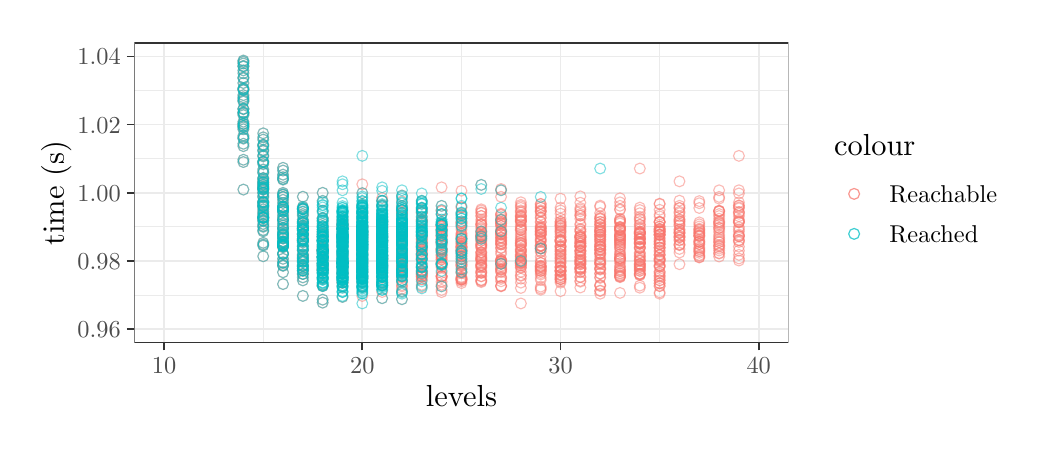
\begin{tikzpicture}[x=1pt,y=1pt]
\definecolor{fillColor}{RGB}{255,255,255}
\path[use as bounding box,fill=fillColor,fill opacity=0.00] (0,0) rectangle (361.35,144.54);
\begin{scope}
\path[clip] (  0.00,  0.00) rectangle (361.35,144.54);
\definecolor{drawColor}{RGB}{255,255,255}
\definecolor{fillColor}{RGB}{255,255,255}

\path[draw=drawColor,line width= 0.6pt,line join=round,line cap=round,fill=fillColor] (  0.00,  0.00) rectangle (361.35,144.54);
\end{scope}
\begin{scope}
\path[clip] ( 38.56, 30.69) rectangle (274.92,139.04);
\definecolor{fillColor}{RGB}{255,255,255}

\path[fill=fillColor] ( 38.56, 30.69) rectangle (274.92,139.04);
\definecolor{drawColor}{gray}{0.92}

\path[draw=drawColor,line width= 0.3pt,line join=round] ( 38.56, 47.92) --
	(274.92, 47.92);

\path[draw=drawColor,line width= 0.3pt,line join=round] ( 38.56, 72.55) --
	(274.92, 72.55);

\path[draw=drawColor,line width= 0.3pt,line join=round] ( 38.56, 97.18) --
	(274.92, 97.18);

\path[draw=drawColor,line width= 0.3pt,line join=round] ( 38.56,121.80) --
	(274.92,121.80);

\path[draw=drawColor,line width= 0.3pt,line join=round] ( 85.11, 30.69) --
	( 85.11,139.04);

\path[draw=drawColor,line width= 0.3pt,line join=round] (156.74, 30.69) --
	(156.74,139.04);

\path[draw=drawColor,line width= 0.3pt,line join=round] (228.36, 30.69) --
	(228.36,139.04);

\path[draw=drawColor,line width= 0.6pt,line join=round] ( 38.56, 35.61) --
	(274.92, 35.61);

\path[draw=drawColor,line width= 0.6pt,line join=round] ( 38.56, 60.24) --
	(274.92, 60.24);

\path[draw=drawColor,line width= 0.6pt,line join=round] ( 38.56, 84.86) --
	(274.92, 84.86);

\path[draw=drawColor,line width= 0.6pt,line join=round] ( 38.56,109.49) --
	(274.92,109.49);

\path[draw=drawColor,line width= 0.6pt,line join=round] ( 38.56,134.11) --
	(274.92,134.11);

\path[draw=drawColor,line width= 0.6pt,line join=round] ( 49.30, 30.69) --
	( 49.30,139.04);

\path[draw=drawColor,line width= 0.6pt,line join=round] (120.92, 30.69) --
	(120.92,139.04);

\path[draw=drawColor,line width= 0.6pt,line join=round] (192.55, 30.69) --
	(192.55,139.04);

\path[draw=drawColor,line width= 0.6pt,line join=round] (264.17, 30.69) --
	(264.17,139.04);
\definecolor{drawColor}{RGB}{248,118,109}

\path[draw=drawColor,draw opacity=0.50,line width= 0.4pt,line join=round,line cap=round] ( 77.95,113.96) circle (  1.96);

\path[draw=drawColor,draw opacity=0.50,line width= 0.4pt,line join=round,line cap=round] ( 77.95,130.49) circle (  1.96);

\path[draw=drawColor,draw opacity=0.50,line width= 0.4pt,line join=round,line cap=round] ( 77.95,109.85) circle (  1.96);

\path[draw=drawColor,draw opacity=0.50,line width= 0.4pt,line join=round,line cap=round] ( 77.95,122.17) circle (  1.96);

\path[draw=drawColor,draw opacity=0.50,line width= 0.4pt,line join=round,line cap=round] ( 77.95,119.40) circle (  1.96);

\path[draw=drawColor,draw opacity=0.50,line width= 0.4pt,line join=round,line cap=round] ( 77.95,126.59) circle (  1.96);

\path[draw=drawColor,draw opacity=0.50,line width= 0.4pt,line join=round,line cap=round] ( 77.95,105.45) circle (  1.96);

\path[draw=drawColor,draw opacity=0.50,line width= 0.4pt,line join=round,line cap=round] ( 77.95,107.83) circle (  1.96);

\path[draw=drawColor,draw opacity=0.50,line width= 0.4pt,line join=round,line cap=round] ( 77.95,132.19) circle (  1.96);

\path[draw=drawColor,draw opacity=0.50,line width= 0.4pt,line join=round,line cap=round] ( 77.95,112.94) circle (  1.96);

\path[draw=drawColor,draw opacity=0.50,line width= 0.4pt,line join=round,line cap=round] ( 77.95,108.52) circle (  1.96);

\path[draw=drawColor,draw opacity=0.50,line width= 0.4pt,line join=round,line cap=round] ( 77.95,120.16) circle (  1.96);

\path[draw=drawColor,draw opacity=0.50,line width= 0.4pt,line join=round,line cap=round] ( 77.95,108.95) circle (  1.96);

\path[draw=drawColor,draw opacity=0.50,line width= 0.4pt,line join=round,line cap=round] ( 77.95,132.66) circle (  1.96);

\path[draw=drawColor,draw opacity=0.50,line width= 0.4pt,line join=round,line cap=round] ( 85.11, 76.95) circle (  1.96);

\path[draw=drawColor,draw opacity=0.50,line width= 0.4pt,line join=round,line cap=round] ( 85.11, 75.87) circle (  1.96);

\path[draw=drawColor,draw opacity=0.50,line width= 0.4pt,line join=round,line cap=round] ( 85.11, 81.26) circle (  1.96);

\path[draw=drawColor,draw opacity=0.50,line width= 0.4pt,line join=round,line cap=round] ( 85.11, 83.75) circle (  1.96);

\path[draw=drawColor,draw opacity=0.50,line width= 0.4pt,line join=round,line cap=round] ( 85.11, 90.02) circle (  1.96);

\path[draw=drawColor,draw opacity=0.50,line width= 0.4pt,line join=round,line cap=round] ( 85.11, 86.97) circle (  1.96);

\path[draw=drawColor,draw opacity=0.50,line width= 0.4pt,line join=round,line cap=round] ( 85.11, 87.79) circle (  1.96);

\path[draw=drawColor,draw opacity=0.50,line width= 0.4pt,line join=round,line cap=round] ( 85.11,102.28) circle (  1.96);

\path[draw=drawColor,draw opacity=0.50,line width= 0.4pt,line join=round,line cap=round] ( 85.11, 86.31) circle (  1.96);

\path[draw=drawColor,draw opacity=0.50,line width= 0.4pt,line join=round,line cap=round] ( 85.11, 95.24) circle (  1.96);

\path[draw=drawColor,draw opacity=0.50,line width= 0.4pt,line join=round,line cap=round] ( 85.11, 87.21) circle (  1.96);

\path[draw=drawColor,draw opacity=0.50,line width= 0.4pt,line join=round,line cap=round] ( 85.11, 80.18) circle (  1.96);

\path[draw=drawColor,draw opacity=0.50,line width= 0.4pt,line join=round,line cap=round] ( 85.11, 87.77) circle (  1.96);

\path[draw=drawColor,draw opacity=0.50,line width= 0.4pt,line join=round,line cap=round] ( 85.11,104.90) circle (  1.96);

\path[draw=drawColor,draw opacity=0.50,line width= 0.4pt,line join=round,line cap=round] ( 85.11, 98.38) circle (  1.96);

\path[draw=drawColor,draw opacity=0.50,line width= 0.4pt,line join=round,line cap=round] ( 85.11, 88.61) circle (  1.96);

\path[draw=drawColor,draw opacity=0.50,line width= 0.4pt,line join=round,line cap=round] ( 85.11, 77.45) circle (  1.96);

\path[draw=drawColor,draw opacity=0.50,line width= 0.4pt,line join=round,line cap=round] ( 85.11,102.11) circle (  1.96);

\path[draw=drawColor,draw opacity=0.50,line width= 0.4pt,line join=round,line cap=round] ( 85.11,100.33) circle (  1.96);

\path[draw=drawColor,draw opacity=0.50,line width= 0.4pt,line join=round,line cap=round] ( 85.11, 88.82) circle (  1.96);

\path[draw=drawColor,draw opacity=0.50,line width= 0.4pt,line join=round,line cap=round] ( 85.11, 98.04) circle (  1.96);

\path[draw=drawColor,draw opacity=0.50,line width= 0.4pt,line join=round,line cap=round] ( 85.11, 93.29) circle (  1.96);

\path[draw=drawColor,draw opacity=0.50,line width= 0.4pt,line join=round,line cap=round] ( 85.11,104.09) circle (  1.96);

\path[draw=drawColor,draw opacity=0.50,line width= 0.4pt,line join=round,line cap=round] ( 85.11, 85.97) circle (  1.96);

\path[draw=drawColor,draw opacity=0.50,line width= 0.4pt,line join=round,line cap=round] ( 85.11, 92.05) circle (  1.96);

\path[draw=drawColor,draw opacity=0.50,line width= 0.4pt,line join=round,line cap=round] ( 85.11, 89.45) circle (  1.96);

\path[draw=drawColor,draw opacity=0.50,line width= 0.4pt,line join=round,line cap=round] ( 85.11, 86.15) circle (  1.96);

\path[draw=drawColor,draw opacity=0.50,line width= 0.4pt,line join=round,line cap=round] ( 85.11, 96.26) circle (  1.96);

\path[draw=drawColor,draw opacity=0.50,line width= 0.4pt,line join=round,line cap=round] ( 85.11, 90.23) circle (  1.96);

\path[draw=drawColor,draw opacity=0.50,line width= 0.4pt,line join=round,line cap=round] ( 85.11, 79.65) circle (  1.96);

\path[draw=drawColor,draw opacity=0.50,line width= 0.4pt,line join=round,line cap=round] ( 85.11, 95.88) circle (  1.96);

\path[draw=drawColor,draw opacity=0.50,line width= 0.4pt,line join=round,line cap=round] ( 85.11,101.69) circle (  1.96);

\path[draw=drawColor,draw opacity=0.50,line width= 0.4pt,line join=round,line cap=round] ( 85.11, 84.88) circle (  1.96);

\path[draw=drawColor,draw opacity=0.50,line width= 0.4pt,line join=round,line cap=round] ( 92.27, 70.41) circle (  1.96);

\path[draw=drawColor,draw opacity=0.50,line width= 0.4pt,line join=round,line cap=round] ( 92.27, 78.79) circle (  1.96);

\path[draw=drawColor,draw opacity=0.50,line width= 0.4pt,line join=round,line cap=round] ( 92.27, 78.53) circle (  1.96);

\path[draw=drawColor,draw opacity=0.50,line width= 0.4pt,line join=round,line cap=round] ( 92.27, 83.47) circle (  1.96);

\path[draw=drawColor,draw opacity=0.50,line width= 0.4pt,line join=round,line cap=round] ( 92.27, 68.42) circle (  1.96);

\path[draw=drawColor,draw opacity=0.50,line width= 0.4pt,line join=round,line cap=round] ( 92.27, 82.33) circle (  1.96);

\path[draw=drawColor,draw opacity=0.50,line width= 0.4pt,line join=round,line cap=round] ( 92.27, 93.89) circle (  1.96);

\path[draw=drawColor,draw opacity=0.50,line width= 0.4pt,line join=round,line cap=round] ( 92.27, 77.98) circle (  1.96);

\path[draw=drawColor,draw opacity=0.50,line width= 0.4pt,line join=round,line cap=round] ( 92.27, 75.15) circle (  1.96);

\path[draw=drawColor,draw opacity=0.50,line width= 0.4pt,line join=round,line cap=round] ( 92.27, 75.99) circle (  1.96);

\path[draw=drawColor,draw opacity=0.50,line width= 0.4pt,line join=round,line cap=round] ( 92.27, 79.91) circle (  1.96);

\path[draw=drawColor,draw opacity=0.50,line width= 0.4pt,line join=round,line cap=round] ( 92.27, 89.90) circle (  1.96);

\path[draw=drawColor,draw opacity=0.50,line width= 0.4pt,line join=round,line cap=round] ( 92.27, 78.94) circle (  1.96);

\path[draw=drawColor,draw opacity=0.50,line width= 0.4pt,line join=round,line cap=round] ( 92.27, 71.78) circle (  1.96);

\path[draw=drawColor,draw opacity=0.50,line width= 0.4pt,line join=round,line cap=round] ( 92.27, 79.42) circle (  1.96);

\path[draw=drawColor,draw opacity=0.50,line width= 0.4pt,line join=round,line cap=round] ( 92.27, 80.01) circle (  1.96);

\path[draw=drawColor,draw opacity=0.50,line width= 0.4pt,line join=round,line cap=round] ( 92.27, 79.59) circle (  1.96);

\path[draw=drawColor,draw opacity=0.50,line width= 0.4pt,line join=round,line cap=round] ( 92.27, 79.67) circle (  1.96);

\path[draw=drawColor,draw opacity=0.50,line width= 0.4pt,line join=round,line cap=round] ( 92.27, 84.84) circle (  1.96);

\path[draw=drawColor,draw opacity=0.50,line width= 0.4pt,line join=round,line cap=round] ( 92.27, 69.88) circle (  1.96);

\path[draw=drawColor,draw opacity=0.50,line width= 0.4pt,line join=round,line cap=round] ( 92.27, 84.31) circle (  1.96);

\path[draw=drawColor,draw opacity=0.50,line width= 0.4pt,line join=round,line cap=round] ( 92.27, 76.81) circle (  1.96);

\path[draw=drawColor,draw opacity=0.50,line width= 0.4pt,line join=round,line cap=round] ( 92.27, 78.09) circle (  1.96);

\path[draw=drawColor,draw opacity=0.50,line width= 0.4pt,line join=round,line cap=round] ( 92.27, 73.87) circle (  1.96);

\path[draw=drawColor,draw opacity=0.50,line width= 0.4pt,line join=round,line cap=round] ( 92.27, 90.51) circle (  1.96);

\path[draw=drawColor,draw opacity=0.50,line width= 0.4pt,line join=round,line cap=round] ( 92.27, 92.91) circle (  1.96);

\path[draw=drawColor,draw opacity=0.50,line width= 0.4pt,line join=round,line cap=round] ( 92.27, 69.60) circle (  1.96);

\path[draw=drawColor,draw opacity=0.50,line width= 0.4pt,line join=round,line cap=round] ( 92.27, 84.14) circle (  1.96);

\path[draw=drawColor,draw opacity=0.50,line width= 0.4pt,line join=round,line cap=round] ( 92.27, 66.41) circle (  1.96);

\path[draw=drawColor,draw opacity=0.50,line width= 0.4pt,line join=round,line cap=round] ( 92.27, 89.63) circle (  1.96);

\path[draw=drawColor,draw opacity=0.50,line width= 0.4pt,line join=round,line cap=round] ( 92.27, 91.42) circle (  1.96);

\path[draw=drawColor,draw opacity=0.50,line width= 0.4pt,line join=round,line cap=round] ( 92.27, 73.13) circle (  1.96);

\path[draw=drawColor,draw opacity=0.50,line width= 0.4pt,line join=round,line cap=round] ( 92.27, 75.17) circle (  1.96);

\path[draw=drawColor,draw opacity=0.50,line width= 0.4pt,line join=round,line cap=round] ( 99.44, 67.91) circle (  1.96);

\path[draw=drawColor,draw opacity=0.50,line width= 0.4pt,line join=round,line cap=round] ( 99.44, 79.03) circle (  1.96);

\path[draw=drawColor,draw opacity=0.50,line width= 0.4pt,line join=round,line cap=round] ( 99.44, 67.56) circle (  1.96);

\path[draw=drawColor,draw opacity=0.50,line width= 0.4pt,line join=round,line cap=round] ( 99.44, 70.07) circle (  1.96);

\path[draw=drawColor,draw opacity=0.50,line width= 0.4pt,line join=round,line cap=round] ( 99.44, 68.30) circle (  1.96);

\path[draw=drawColor,draw opacity=0.50,line width= 0.4pt,line join=round,line cap=round] ( 99.44, 72.05) circle (  1.96);

\path[draw=drawColor,draw opacity=0.50,line width= 0.4pt,line join=round,line cap=round] ( 99.44, 64.15) circle (  1.96);

\path[draw=drawColor,draw opacity=0.50,line width= 0.4pt,line join=round,line cap=round] ( 99.44, 74.09) circle (  1.96);

\path[draw=drawColor,draw opacity=0.50,line width= 0.4pt,line join=round,line cap=round] ( 99.44, 78.99) circle (  1.96);

\path[draw=drawColor,draw opacity=0.50,line width= 0.4pt,line join=round,line cap=round] ( 99.44, 72.94) circle (  1.96);

\path[draw=drawColor,draw opacity=0.50,line width= 0.4pt,line join=round,line cap=round] ( 99.44, 78.90) circle (  1.96);

\path[draw=drawColor,draw opacity=0.50,line width= 0.4pt,line join=round,line cap=round] ( 99.44, 74.48) circle (  1.96);

\path[draw=drawColor,draw opacity=0.50,line width= 0.4pt,line join=round,line cap=round] ( 99.44, 68.08) circle (  1.96);

\path[draw=drawColor,draw opacity=0.50,line width= 0.4pt,line join=round,line cap=round] ( 99.44, 75.22) circle (  1.96);

\path[draw=drawColor,draw opacity=0.50,line width= 0.4pt,line join=round,line cap=round] ( 99.44, 77.20) circle (  1.96);

\path[draw=drawColor,draw opacity=0.50,line width= 0.4pt,line join=round,line cap=round] ( 99.44, 77.95) circle (  1.96);

\path[draw=drawColor,draw opacity=0.50,line width= 0.4pt,line join=round,line cap=round] ( 99.44, 73.96) circle (  1.96);

\path[draw=drawColor,draw opacity=0.50,line width= 0.4pt,line join=round,line cap=round] ( 99.44, 79.32) circle (  1.96);

\path[draw=drawColor,draw opacity=0.50,line width= 0.4pt,line join=round,line cap=round] ( 99.44, 64.46) circle (  1.96);

\path[draw=drawColor,draw opacity=0.50,line width= 0.4pt,line join=round,line cap=round] ( 99.44, 66.92) circle (  1.96);

\path[draw=drawColor,draw opacity=0.50,line width= 0.4pt,line join=round,line cap=round] ( 99.44, 72.50) circle (  1.96);

\path[draw=drawColor,draw opacity=0.50,line width= 0.4pt,line join=round,line cap=round] ( 99.44, 69.88) circle (  1.96);

\path[draw=drawColor,draw opacity=0.50,line width= 0.4pt,line join=round,line cap=round] ( 99.44, 58.83) circle (  1.96);

\path[draw=drawColor,draw opacity=0.50,line width= 0.4pt,line join=round,line cap=round] ( 99.44, 71.97) circle (  1.96);

\path[draw=drawColor,draw opacity=0.50,line width= 0.4pt,line join=round,line cap=round] ( 99.44, 69.86) circle (  1.96);

\path[draw=drawColor,draw opacity=0.50,line width= 0.4pt,line join=round,line cap=round] ( 99.44, 69.12) circle (  1.96);

\path[draw=drawColor,draw opacity=0.50,line width= 0.4pt,line join=round,line cap=round] ( 99.44, 79.79) circle (  1.96);

\path[draw=drawColor,draw opacity=0.50,line width= 0.4pt,line join=round,line cap=round] ( 99.44, 71.37) circle (  1.96);

\path[draw=drawColor,draw opacity=0.50,line width= 0.4pt,line join=round,line cap=round] ( 99.44, 73.83) circle (  1.96);

\path[draw=drawColor,draw opacity=0.50,line width= 0.4pt,line join=round,line cap=round] ( 99.44, 72.00) circle (  1.96);

\path[draw=drawColor,draw opacity=0.50,line width= 0.4pt,line join=round,line cap=round] ( 99.44, 72.43) circle (  1.96);

\path[draw=drawColor,draw opacity=0.50,line width= 0.4pt,line join=round,line cap=round] ( 99.44, 61.97) circle (  1.96);

\path[draw=drawColor,draw opacity=0.50,line width= 0.4pt,line join=round,line cap=round] ( 99.44, 65.50) circle (  1.96);

\path[draw=drawColor,draw opacity=0.50,line width= 0.4pt,line join=round,line cap=round] (106.60, 84.86) circle (  1.96);

\path[draw=drawColor,draw opacity=0.50,line width= 0.4pt,line join=round,line cap=round] (106.60, 69.23) circle (  1.96);

\path[draw=drawColor,draw opacity=0.50,line width= 0.4pt,line join=round,line cap=round] (106.60, 67.50) circle (  1.96);

\path[draw=drawColor,draw opacity=0.50,line width= 0.4pt,line join=round,line cap=round] (106.60, 61.84) circle (  1.96);

\path[draw=drawColor,draw opacity=0.50,line width= 0.4pt,line join=round,line cap=round] (106.60, 67.71) circle (  1.96);

\path[draw=drawColor,draw opacity=0.50,line width= 0.4pt,line join=round,line cap=round] (106.60, 68.29) circle (  1.96);

\path[draw=drawColor,draw opacity=0.50,line width= 0.4pt,line join=round,line cap=round] (106.60, 74.70) circle (  1.96);

\path[draw=drawColor,draw opacity=0.50,line width= 0.4pt,line join=round,line cap=round] (106.60, 64.10) circle (  1.96);

\path[draw=drawColor,draw opacity=0.50,line width= 0.4pt,line join=round,line cap=round] (106.60, 67.83) circle (  1.96);

\path[draw=drawColor,draw opacity=0.50,line width= 0.4pt,line join=round,line cap=round] (106.60, 68.92) circle (  1.96);

\path[draw=drawColor,draw opacity=0.50,line width= 0.4pt,line join=round,line cap=round] (106.60, 64.83) circle (  1.96);

\path[draw=drawColor,draw opacity=0.50,line width= 0.4pt,line join=round,line cap=round] (106.60, 70.13) circle (  1.96);

\path[draw=drawColor,draw opacity=0.50,line width= 0.4pt,line join=round,line cap=round] (106.60, 69.85) circle (  1.96);

\path[draw=drawColor,draw opacity=0.50,line width= 0.4pt,line join=round,line cap=round] (106.60, 61.92) circle (  1.96);

\path[draw=drawColor,draw opacity=0.50,line width= 0.4pt,line join=round,line cap=round] (106.60, 57.52) circle (  1.96);

\path[draw=drawColor,draw opacity=0.50,line width= 0.4pt,line join=round,line cap=round] (106.60, 63.13) circle (  1.96);

\path[draw=drawColor,draw opacity=0.50,line width= 0.4pt,line join=round,line cap=round] (106.60, 63.43) circle (  1.96);

\path[draw=drawColor,draw opacity=0.50,line width= 0.4pt,line join=round,line cap=round] (106.60, 70.70) circle (  1.96);

\path[draw=drawColor,draw opacity=0.50,line width= 0.4pt,line join=round,line cap=round] (106.60, 68.92) circle (  1.96);

\path[draw=drawColor,draw opacity=0.50,line width= 0.4pt,line join=round,line cap=round] (106.60, 75.60) circle (  1.96);

\path[draw=drawColor,draw opacity=0.50,line width= 0.4pt,line join=round,line cap=round] (106.60, 61.30) circle (  1.96);

\path[draw=drawColor,draw opacity=0.50,line width= 0.4pt,line join=round,line cap=round] (106.60, 65.09) circle (  1.96);

\path[draw=drawColor,draw opacity=0.50,line width= 0.4pt,line join=round,line cap=round] (106.60, 75.78) circle (  1.96);

\path[draw=drawColor,draw opacity=0.50,line width= 0.4pt,line join=round,line cap=round] (106.60, 63.87) circle (  1.96);

\path[draw=drawColor,draw opacity=0.50,line width= 0.4pt,line join=round,line cap=round] (106.60, 73.62) circle (  1.96);

\path[draw=drawColor,draw opacity=0.50,line width= 0.4pt,line join=round,line cap=round] (106.60, 67.30) circle (  1.96);

\path[draw=drawColor,draw opacity=0.50,line width= 0.4pt,line join=round,line cap=round] (106.60, 65.39) circle (  1.96);

\path[draw=drawColor,draw opacity=0.50,line width= 0.4pt,line join=round,line cap=round] (106.60, 81.95) circle (  1.96);

\path[draw=drawColor,draw opacity=0.50,line width= 0.4pt,line join=round,line cap=round] (106.60, 63.78) circle (  1.96);

\path[draw=drawColor,draw opacity=0.50,line width= 0.4pt,line join=round,line cap=round] (106.60, 64.41) circle (  1.96);

\path[draw=drawColor,draw opacity=0.50,line width= 0.4pt,line join=round,line cap=round] (106.60, 62.75) circle (  1.96);

\path[draw=drawColor,draw opacity=0.50,line width= 0.4pt,line join=round,line cap=round] (106.60, 64.16) circle (  1.96);

\path[draw=drawColor,draw opacity=0.50,line width= 0.4pt,line join=round,line cap=round] (106.60, 69.00) circle (  1.96);

\path[draw=drawColor,draw opacity=0.50,line width= 0.4pt,line join=round,line cap=round] (113.76, 72.97) circle (  1.96);

\path[draw=drawColor,draw opacity=0.50,line width= 0.4pt,line join=round,line cap=round] (113.76, 73.76) circle (  1.96);

\path[draw=drawColor,draw opacity=0.50,line width= 0.4pt,line join=round,line cap=round] (113.76, 59.34) circle (  1.96);

\path[draw=drawColor,draw opacity=0.50,line width= 0.4pt,line join=round,line cap=round] (113.76, 70.00) circle (  1.96);

\path[draw=drawColor,draw opacity=0.50,line width= 0.4pt,line join=round,line cap=round] (113.76, 69.71) circle (  1.96);

\path[draw=drawColor,draw opacity=0.50,line width= 0.4pt,line join=round,line cap=round] (113.76, 69.31) circle (  1.96);

\path[draw=drawColor,draw opacity=0.50,line width= 0.4pt,line join=round,line cap=round] (113.76, 66.32) circle (  1.96);

\path[draw=drawColor,draw opacity=0.50,line width= 0.4pt,line join=round,line cap=round] (113.76, 58.16) circle (  1.96);

\path[draw=drawColor,draw opacity=0.50,line width= 0.4pt,line join=round,line cap=round] (113.76, 65.86) circle (  1.96);

\path[draw=drawColor,draw opacity=0.50,line width= 0.4pt,line join=round,line cap=round] (113.76, 66.92) circle (  1.96);

\path[draw=drawColor,draw opacity=0.50,line width= 0.4pt,line join=round,line cap=round] (113.76, 73.41) circle (  1.96);

\path[draw=drawColor,draw opacity=0.50,line width= 0.4pt,line join=round,line cap=round] (113.76, 73.18) circle (  1.96);

\path[draw=drawColor,draw opacity=0.50,line width= 0.4pt,line join=round,line cap=round] (113.76, 64.26) circle (  1.96);

\path[draw=drawColor,draw opacity=0.50,line width= 0.4pt,line join=round,line cap=round] (113.76, 73.17) circle (  1.96);

\path[draw=drawColor,draw opacity=0.50,line width= 0.4pt,line join=round,line cap=round] (113.76, 74.43) circle (  1.96);

\path[draw=drawColor,draw opacity=0.50,line width= 0.4pt,line join=round,line cap=round] (113.76, 63.01) circle (  1.96);

\path[draw=drawColor,draw opacity=0.50,line width= 0.4pt,line join=round,line cap=round] (113.76, 72.00) circle (  1.96);

\path[draw=drawColor,draw opacity=0.50,line width= 0.4pt,line join=round,line cap=round] (113.76, 74.87) circle (  1.96);

\path[draw=drawColor,draw opacity=0.50,line width= 0.4pt,line join=round,line cap=round] (113.76, 72.02) circle (  1.96);

\path[draw=drawColor,draw opacity=0.50,line width= 0.4pt,line join=round,line cap=round] (113.76, 73.81) circle (  1.96);

\path[draw=drawColor,draw opacity=0.50,line width= 0.4pt,line join=round,line cap=round] (113.76, 75.99) circle (  1.96);

\path[draw=drawColor,draw opacity=0.50,line width= 0.4pt,line join=round,line cap=round] (113.76, 69.82) circle (  1.96);

\path[draw=drawColor,draw opacity=0.50,line width= 0.4pt,line join=round,line cap=round] (113.76, 71.72) circle (  1.96);

\path[draw=drawColor,draw opacity=0.50,line width= 0.4pt,line join=round,line cap=round] (113.76, 69.07) circle (  1.96);

\path[draw=drawColor,draw opacity=0.50,line width= 0.4pt,line join=round,line cap=round] (113.76, 73.58) circle (  1.96);

\path[draw=drawColor,draw opacity=0.50,line width= 0.4pt,line join=round,line cap=round] (113.76, 72.53) circle (  1.96);

\path[draw=drawColor,draw opacity=0.50,line width= 0.4pt,line join=round,line cap=round] (113.76, 67.25) circle (  1.96);

\path[draw=drawColor,draw opacity=0.50,line width= 0.4pt,line join=round,line cap=round] (113.76, 61.97) circle (  1.96);

\path[draw=drawColor,draw opacity=0.50,line width= 0.4pt,line join=round,line cap=round] (113.76, 63.63) circle (  1.96);

\path[draw=drawColor,draw opacity=0.50,line width= 0.4pt,line join=round,line cap=round] (113.76, 71.67) circle (  1.96);

\path[draw=drawColor,draw opacity=0.50,line width= 0.4pt,line join=round,line cap=round] (113.76, 74.96) circle (  1.96);

\path[draw=drawColor,draw opacity=0.50,line width= 0.4pt,line join=round,line cap=round] (113.76, 62.17) circle (  1.96);

\path[draw=drawColor,draw opacity=0.50,line width= 0.4pt,line join=round,line cap=round] (113.76, 58.93) circle (  1.96);

\path[draw=drawColor,draw opacity=0.50,line width= 0.4pt,line join=round,line cap=round] (120.92, 64.10) circle (  1.96);

\path[draw=drawColor,draw opacity=0.50,line width= 0.4pt,line join=round,line cap=round] (120.92, 68.22) circle (  1.96);

\path[draw=drawColor,draw opacity=0.50,line width= 0.4pt,line join=round,line cap=round] (120.92, 78.12) circle (  1.96);

\path[draw=drawColor,draw opacity=0.50,line width= 0.4pt,line join=round,line cap=round] (120.92, 69.50) circle (  1.96);

\path[draw=drawColor,draw opacity=0.50,line width= 0.4pt,line join=round,line cap=round] (120.92, 72.93) circle (  1.96);

\path[draw=drawColor,draw opacity=0.50,line width= 0.4pt,line join=round,line cap=round] (120.92, 72.69) circle (  1.96);

\path[draw=drawColor,draw opacity=0.50,line width= 0.4pt,line join=round,line cap=round] (120.92, 63.97) circle (  1.96);

\path[draw=drawColor,draw opacity=0.50,line width= 0.4pt,line join=round,line cap=round] (120.92, 77.37) circle (  1.96);

\path[draw=drawColor,draw opacity=0.50,line width= 0.4pt,line join=round,line cap=round] (120.92, 72.46) circle (  1.96);

\path[draw=drawColor,draw opacity=0.50,line width= 0.4pt,line join=round,line cap=round] (120.92, 67.71) circle (  1.96);

\path[draw=drawColor,draw opacity=0.50,line width= 0.4pt,line join=round,line cap=round] (120.92, 64.58) circle (  1.96);

\path[draw=drawColor,draw opacity=0.50,line width= 0.4pt,line join=round,line cap=round] (120.92, 61.99) circle (  1.96);

\path[draw=drawColor,draw opacity=0.50,line width= 0.4pt,line join=round,line cap=round] (120.92, 75.33) circle (  1.96);

\path[draw=drawColor,draw opacity=0.50,line width= 0.4pt,line join=round,line cap=round] (120.92, 69.23) circle (  1.96);

\path[draw=drawColor,draw opacity=0.50,line width= 0.4pt,line join=round,line cap=round] (120.92, 77.45) circle (  1.96);

\path[draw=drawColor,draw opacity=0.50,line width= 0.4pt,line join=round,line cap=round] (120.92, 68.49) circle (  1.96);

\path[draw=drawColor,draw opacity=0.50,line width= 0.4pt,line join=round,line cap=round] (120.92, 72.40) circle (  1.96);

\path[draw=drawColor,draw opacity=0.50,line width= 0.4pt,line join=round,line cap=round] (120.92, 74.89) circle (  1.96);

\path[draw=drawColor,draw opacity=0.50,line width= 0.4pt,line join=round,line cap=round] (120.92, 59.88) circle (  1.96);

\path[draw=drawColor,draw opacity=0.50,line width= 0.4pt,line join=round,line cap=round] (120.92, 68.66) circle (  1.96);

\path[draw=drawColor,draw opacity=0.50,line width= 0.4pt,line join=round,line cap=round] (120.92, 69.75) circle (  1.96);

\path[draw=drawColor,draw opacity=0.50,line width= 0.4pt,line join=round,line cap=round] (120.92, 70.73) circle (  1.96);

\path[draw=drawColor,draw opacity=0.50,line width= 0.4pt,line join=round,line cap=round] (120.92, 71.02) circle (  1.96);

\path[draw=drawColor,draw opacity=0.50,line width= 0.4pt,line join=round,line cap=round] (120.92, 70.00) circle (  1.96);

\path[draw=drawColor,draw opacity=0.50,line width= 0.4pt,line join=round,line cap=round] (120.92, 84.74) circle (  1.96);

\path[draw=drawColor,draw opacity=0.50,line width= 0.4pt,line join=round,line cap=round] (120.92, 87.96) circle (  1.96);

\path[draw=drawColor,draw opacity=0.50,line width= 0.4pt,line join=round,line cap=round] (120.92, 80.52) circle (  1.96);

\path[draw=drawColor,draw opacity=0.50,line width= 0.4pt,line join=round,line cap=round] (120.92, 69.86) circle (  1.96);

\path[draw=drawColor,draw opacity=0.50,line width= 0.4pt,line join=round,line cap=round] (120.92, 70.85) circle (  1.96);

\path[draw=drawColor,draw opacity=0.50,line width= 0.4pt,line join=round,line cap=round] (120.92, 63.51) circle (  1.96);

\path[draw=drawColor,draw opacity=0.50,line width= 0.4pt,line join=round,line cap=round] (120.92, 72.55) circle (  1.96);

\path[draw=drawColor,draw opacity=0.50,line width= 0.4pt,line join=round,line cap=round] (120.92, 69.61) circle (  1.96);

\path[draw=drawColor,draw opacity=0.50,line width= 0.4pt,line join=round,line cap=round] (120.92, 68.57) circle (  1.96);

\path[draw=drawColor,draw opacity=0.50,line width= 0.4pt,line join=round,line cap=round] (128.09, 69.06) circle (  1.96);

\path[draw=drawColor,draw opacity=0.50,line width= 0.4pt,line join=round,line cap=round] (128.09, 78.39) circle (  1.96);

\path[draw=drawColor,draw opacity=0.50,line width= 0.4pt,line join=round,line cap=round] (128.09, 80.40) circle (  1.96);

\path[draw=drawColor,draw opacity=0.50,line width= 0.4pt,line join=round,line cap=round] (128.09, 67.59) circle (  1.96);

\path[draw=drawColor,draw opacity=0.50,line width= 0.4pt,line join=round,line cap=round] (128.09, 63.48) circle (  1.96);

\path[draw=drawColor,draw opacity=0.50,line width= 0.4pt,line join=round,line cap=round] (128.09, 70.26) circle (  1.96);

\path[draw=drawColor,draw opacity=0.50,line width= 0.4pt,line join=round,line cap=round] (128.09, 64.89) circle (  1.96);

\path[draw=drawColor,draw opacity=0.50,line width= 0.4pt,line join=round,line cap=round] (128.09, 61.75) circle (  1.96);

\path[draw=drawColor,draw opacity=0.50,line width= 0.4pt,line join=round,line cap=round] (128.09, 68.85) circle (  1.96);

\path[draw=drawColor,draw opacity=0.50,line width= 0.4pt,line join=round,line cap=round] (128.09, 81.97) circle (  1.96);

\path[draw=drawColor,draw opacity=0.50,line width= 0.4pt,line join=round,line cap=round] (128.09, 68.69) circle (  1.96);

\path[draw=drawColor,draw opacity=0.50,line width= 0.4pt,line join=round,line cap=round] (128.09, 81.95) circle (  1.96);

\path[draw=drawColor,draw opacity=0.50,line width= 0.4pt,line join=round,line cap=round] (128.09, 64.37) circle (  1.96);

\path[draw=drawColor,draw opacity=0.50,line width= 0.4pt,line join=round,line cap=round] (128.09, 72.50) circle (  1.96);

\path[draw=drawColor,draw opacity=0.50,line width= 0.4pt,line join=round,line cap=round] (128.09, 67.31) circle (  1.96);

\path[draw=drawColor,draw opacity=0.50,line width= 0.4pt,line join=round,line cap=round] (128.09, 73.01) circle (  1.96);

\path[draw=drawColor,draw opacity=0.50,line width= 0.4pt,line join=round,line cap=round] (128.09, 68.95) circle (  1.96);

\path[draw=drawColor,draw opacity=0.50,line width= 0.4pt,line join=round,line cap=round] (128.09, 66.82) circle (  1.96);

\path[draw=drawColor,draw opacity=0.50,line width= 0.4pt,line join=round,line cap=round] (128.09, 80.12) circle (  1.96);

\path[draw=drawColor,draw opacity=0.50,line width= 0.4pt,line join=round,line cap=round] (128.09, 73.98) circle (  1.96);

\path[draw=drawColor,draw opacity=0.50,line width= 0.4pt,line join=round,line cap=round] (128.09, 62.19) circle (  1.96);

\path[draw=drawColor,draw opacity=0.50,line width= 0.4pt,line join=round,line cap=round] (128.09, 72.37) circle (  1.96);

\path[draw=drawColor,draw opacity=0.50,line width= 0.4pt,line join=round,line cap=round] (128.09, 67.78) circle (  1.96);

\path[draw=drawColor,draw opacity=0.50,line width= 0.4pt,line join=round,line cap=round] (128.09, 73.56) circle (  1.96);

\path[draw=drawColor,draw opacity=0.50,line width= 0.4pt,line join=round,line cap=round] (128.09, 68.09) circle (  1.96);

\path[draw=drawColor,draw opacity=0.50,line width= 0.4pt,line join=round,line cap=round] (128.09, 69.95) circle (  1.96);

\path[draw=drawColor,draw opacity=0.50,line width= 0.4pt,line join=round,line cap=round] (128.09, 62.30) circle (  1.96);

\path[draw=drawColor,draw opacity=0.50,line width= 0.4pt,line join=round,line cap=round] (128.09, 82.98) circle (  1.96);

\path[draw=drawColor,draw opacity=0.50,line width= 0.4pt,line join=round,line cap=round] (128.09, 71.46) circle (  1.96);

\path[draw=drawColor,draw opacity=0.50,line width= 0.4pt,line join=round,line cap=round] (128.09, 72.14) circle (  1.96);

\path[draw=drawColor,draw opacity=0.50,line width= 0.4pt,line join=round,line cap=round] (128.09, 74.04) circle (  1.96);

\path[draw=drawColor,draw opacity=0.50,line width= 0.4pt,line join=round,line cap=round] (128.09, 73.12) circle (  1.96);

\path[draw=drawColor,draw opacity=0.50,line width= 0.4pt,line join=round,line cap=round] (128.09, 76.26) circle (  1.96);

\path[draw=drawColor,draw opacity=0.50,line width= 0.4pt,line join=round,line cap=round] (135.25, 77.78) circle (  1.96);

\path[draw=drawColor,draw opacity=0.50,line width= 0.4pt,line join=round,line cap=round] (135.25, 75.36) circle (  1.96);

\path[draw=drawColor,draw opacity=0.50,line width= 0.4pt,line join=round,line cap=round] (135.25, 70.66) circle (  1.96);

\path[draw=drawColor,draw opacity=0.50,line width= 0.4pt,line join=round,line cap=round] (135.25, 64.85) circle (  1.96);

\path[draw=drawColor,draw opacity=0.50,line width= 0.4pt,line join=round,line cap=round] (135.25, 69.24) circle (  1.96);

\path[draw=drawColor,draw opacity=0.50,line width= 0.4pt,line join=round,line cap=round] (135.25, 75.95) circle (  1.96);

\path[draw=drawColor,draw opacity=0.50,line width= 0.4pt,line join=round,line cap=round] (135.25, 78.76) circle (  1.96);

\path[draw=drawColor,draw opacity=0.50,line width= 0.4pt,line join=round,line cap=round] (135.25, 77.54) circle (  1.96);

\path[draw=drawColor,draw opacity=0.50,line width= 0.4pt,line join=round,line cap=round] (135.25, 58.90) circle (  1.96);

\path[draw=drawColor,draw opacity=0.50,line width= 0.4pt,line join=round,line cap=round] (135.25, 68.16) circle (  1.96);

\path[draw=drawColor,draw opacity=0.50,line width= 0.4pt,line join=round,line cap=round] (135.25, 78.51) circle (  1.96);

\path[draw=drawColor,draw opacity=0.50,line width= 0.4pt,line join=round,line cap=round] (135.25, 83.89) circle (  1.96);

\path[draw=drawColor,draw opacity=0.50,line width= 0.4pt,line join=round,line cap=round] (135.25, 62.98) circle (  1.96);

\path[draw=drawColor,draw opacity=0.50,line width= 0.4pt,line join=round,line cap=round] (135.25, 62.54) circle (  1.96);

\path[draw=drawColor,draw opacity=0.50,line width= 0.4pt,line join=round,line cap=round] (135.25, 67.19) circle (  1.96);

\path[draw=drawColor,draw opacity=0.50,line width= 0.4pt,line join=round,line cap=round] (135.25, 79.48) circle (  1.96);

\path[draw=drawColor,draw opacity=0.50,line width= 0.4pt,line join=round,line cap=round] (135.25, 71.87) circle (  1.96);

\path[draw=drawColor,draw opacity=0.50,line width= 0.4pt,line join=round,line cap=round] (135.25, 69.95) circle (  1.96);

\path[draw=drawColor,draw opacity=0.50,line width= 0.4pt,line join=round,line cap=round] (135.25, 72.50) circle (  1.96);

\path[draw=drawColor,draw opacity=0.50,line width= 0.4pt,line join=round,line cap=round] (135.25, 66.69) circle (  1.96);

\path[draw=drawColor,draw opacity=0.50,line width= 0.4pt,line join=round,line cap=round] (135.25, 69.07) circle (  1.96);

\path[draw=drawColor,draw opacity=0.50,line width= 0.4pt,line join=round,line cap=round] (135.25, 63.18) circle (  1.96);

\path[draw=drawColor,draw opacity=0.50,line width= 0.4pt,line join=round,line cap=round] (135.25, 71.24) circle (  1.96);

\path[draw=drawColor,draw opacity=0.50,line width= 0.4pt,line join=round,line cap=round] (135.25, 80.07) circle (  1.96);

\path[draw=drawColor,draw opacity=0.50,line width= 0.4pt,line join=round,line cap=round] (135.25, 70.17) circle (  1.96);

\path[draw=drawColor,draw opacity=0.50,line width= 0.4pt,line join=round,line cap=round] (135.25, 65.86) circle (  1.96);

\path[draw=drawColor,draw opacity=0.50,line width= 0.4pt,line join=round,line cap=round] (135.25, 70.89) circle (  1.96);

\path[draw=drawColor,draw opacity=0.50,line width= 0.4pt,line join=round,line cap=round] (135.25, 69.86) circle (  1.96);

\path[draw=drawColor,draw opacity=0.50,line width= 0.4pt,line join=round,line cap=round] (135.25, 68.60) circle (  1.96);

\path[draw=drawColor,draw opacity=0.50,line width= 0.4pt,line join=round,line cap=round] (135.25, 67.67) circle (  1.96);

\path[draw=drawColor,draw opacity=0.50,line width= 0.4pt,line join=round,line cap=round] (135.25, 77.65) circle (  1.96);

\path[draw=drawColor,draw opacity=0.50,line width= 0.4pt,line join=round,line cap=round] (135.25, 71.48) circle (  1.96);

\path[draw=drawColor,draw opacity=0.50,line width= 0.4pt,line join=round,line cap=round] (135.25, 66.56) circle (  1.96);

\path[draw=drawColor,draw opacity=0.50,line width= 0.4pt,line join=round,line cap=round] (142.41, 77.55) circle (  1.96);

\path[draw=drawColor,draw opacity=0.50,line width= 0.4pt,line join=round,line cap=round] (142.41, 73.24) circle (  1.96);

\path[draw=drawColor,draw opacity=0.50,line width= 0.4pt,line join=round,line cap=round] (142.41, 71.39) circle (  1.96);

\path[draw=drawColor,draw opacity=0.50,line width= 0.4pt,line join=round,line cap=round] (142.41, 74.98) circle (  1.96);

\path[draw=drawColor,draw opacity=0.50,line width= 0.4pt,line join=round,line cap=round] (142.41, 69.57) circle (  1.96);

\path[draw=drawColor,draw opacity=0.50,line width= 0.4pt,line join=round,line cap=round] (142.41, 73.86) circle (  1.96);

\path[draw=drawColor,draw opacity=0.50,line width= 0.4pt,line join=round,line cap=round] (142.41, 67.48) circle (  1.96);

\path[draw=drawColor,draw opacity=0.50,line width= 0.4pt,line join=round,line cap=round] (142.41, 69.10) circle (  1.96);

\path[draw=drawColor,draw opacity=0.50,line width= 0.4pt,line join=round,line cap=round] (142.41, 76.00) circle (  1.96);

\path[draw=drawColor,draw opacity=0.50,line width= 0.4pt,line join=round,line cap=round] (142.41, 62.26) circle (  1.96);

\path[draw=drawColor,draw opacity=0.50,line width= 0.4pt,line join=round,line cap=round] (142.41, 74.34) circle (  1.96);

\path[draw=drawColor,draw opacity=0.50,line width= 0.4pt,line join=round,line cap=round] (142.41, 79.41) circle (  1.96);

\path[draw=drawColor,draw opacity=0.50,line width= 0.4pt,line join=round,line cap=round] (142.41, 66.78) circle (  1.96);

\path[draw=drawColor,draw opacity=0.50,line width= 0.4pt,line join=round,line cap=round] (142.41, 75.14) circle (  1.96);

\path[draw=drawColor,draw opacity=0.50,line width= 0.4pt,line join=round,line cap=round] (142.41, 69.35) circle (  1.96);

\path[draw=drawColor,draw opacity=0.50,line width= 0.4pt,line join=round,line cap=round] (142.41, 67.27) circle (  1.96);

\path[draw=drawColor,draw opacity=0.50,line width= 0.4pt,line join=round,line cap=round] (142.41, 68.06) circle (  1.96);

\path[draw=drawColor,draw opacity=0.50,line width= 0.4pt,line join=round,line cap=round] (142.41, 70.61) circle (  1.96);

\path[draw=drawColor,draw opacity=0.50,line width= 0.4pt,line join=round,line cap=round] (142.41, 74.62) circle (  1.96);

\path[draw=drawColor,draw opacity=0.50,line width= 0.4pt,line join=round,line cap=round] (142.41, 81.94) circle (  1.96);

\path[draw=drawColor,draw opacity=0.50,line width= 0.4pt,line join=round,line cap=round] (142.41, 64.50) circle (  1.96);

\path[draw=drawColor,draw opacity=0.50,line width= 0.4pt,line join=round,line cap=round] (142.41, 65.35) circle (  1.96);

\path[draw=drawColor,draw opacity=0.50,line width= 0.4pt,line join=round,line cap=round] (142.41, 77.65) circle (  1.96);

\path[draw=drawColor,draw opacity=0.50,line width= 0.4pt,line join=round,line cap=round] (142.41, 66.90) circle (  1.96);

\path[draw=drawColor,draw opacity=0.50,line width= 0.4pt,line join=round,line cap=round] (142.41, 66.23) circle (  1.96);

\path[draw=drawColor,draw opacity=0.50,line width= 0.4pt,line join=round,line cap=round] (142.41, 69.14) circle (  1.96);

\path[draw=drawColor,draw opacity=0.50,line width= 0.4pt,line join=round,line cap=round] (142.41, 74.90) circle (  1.96);

\path[draw=drawColor,draw opacity=0.50,line width= 0.4pt,line join=round,line cap=round] (142.41, 62.79) circle (  1.96);

\path[draw=drawColor,draw opacity=0.50,line width= 0.4pt,line join=round,line cap=round] (142.41, 68.96) circle (  1.96);

\path[draw=drawColor,draw opacity=0.50,line width= 0.4pt,line join=round,line cap=round] (142.41, 67.98) circle (  1.96);

\path[draw=drawColor,draw opacity=0.50,line width= 0.4pt,line join=round,line cap=round] (142.41, 78.73) circle (  1.96);

\path[draw=drawColor,draw opacity=0.50,line width= 0.4pt,line join=round,line cap=round] (142.41, 65.54) circle (  1.96);

\path[draw=drawColor,draw opacity=0.50,line width= 0.4pt,line join=round,line cap=round] (142.41, 65.87) circle (  1.96);

\path[draw=drawColor,draw opacity=0.50,line width= 0.4pt,line join=round,line cap=round] (149.57, 69.70) circle (  1.96);

\path[draw=drawColor,draw opacity=0.50,line width= 0.4pt,line join=round,line cap=round] (149.57, 70.60) circle (  1.96);

\path[draw=drawColor,draw opacity=0.50,line width= 0.4pt,line join=round,line cap=round] (149.57, 78.47) circle (  1.96);

\path[draw=drawColor,draw opacity=0.50,line width= 0.4pt,line join=round,line cap=round] (149.57, 73.94) circle (  1.96);

\path[draw=drawColor,draw opacity=0.50,line width= 0.4pt,line join=round,line cap=round] (149.57, 76.99) circle (  1.96);

\path[draw=drawColor,draw opacity=0.50,line width= 0.4pt,line join=round,line cap=round] (149.57, 69.33) circle (  1.96);

\path[draw=drawColor,draw opacity=0.50,line width= 0.4pt,line join=round,line cap=round] (149.57, 66.99) circle (  1.96);

\path[draw=drawColor,draw opacity=0.50,line width= 0.4pt,line join=round,line cap=round] (149.57, 73.04) circle (  1.96);

\path[draw=drawColor,draw opacity=0.50,line width= 0.4pt,line join=round,line cap=round] (149.57, 58.28) circle (  1.96);

\path[draw=drawColor,draw opacity=0.50,line width= 0.4pt,line join=round,line cap=round] (149.57, 80.12) circle (  1.96);

\path[draw=drawColor,draw opacity=0.50,line width= 0.4pt,line join=round,line cap=round] (149.57, 71.00) circle (  1.96);

\path[draw=drawColor,draw opacity=0.50,line width= 0.4pt,line join=round,line cap=round] (149.57, 61.33) circle (  1.96);

\path[draw=drawColor,draw opacity=0.50,line width= 0.4pt,line join=round,line cap=round] (149.57, 67.13) circle (  1.96);

\path[draw=drawColor,draw opacity=0.50,line width= 0.4pt,line join=round,line cap=round] (149.57, 67.19) circle (  1.96);

\path[draw=drawColor,draw opacity=0.50,line width= 0.4pt,line join=round,line cap=round] (149.57, 71.78) circle (  1.96);

\path[draw=drawColor,draw opacity=0.50,line width= 0.4pt,line join=round,line cap=round] (149.57, 73.19) circle (  1.96);

\path[draw=drawColor,draw opacity=0.50,line width= 0.4pt,line join=round,line cap=round] (149.57, 71.31) circle (  1.96);

\path[draw=drawColor,draw opacity=0.50,line width= 0.4pt,line join=round,line cap=round] (149.57, 70.26) circle (  1.96);

\path[draw=drawColor,draw opacity=0.50,line width= 0.4pt,line join=round,line cap=round] (149.57, 72.06) circle (  1.96);

\path[draw=drawColor,draw opacity=0.50,line width= 0.4pt,line join=round,line cap=round] (149.57, 73.57) circle (  1.96);

\path[draw=drawColor,draw opacity=0.50,line width= 0.4pt,line join=round,line cap=round] (149.57, 73.19) circle (  1.96);

\path[draw=drawColor,draw opacity=0.50,line width= 0.4pt,line join=round,line cap=round] (149.57, 67.17) circle (  1.96);

\path[draw=drawColor,draw opacity=0.50,line width= 0.4pt,line join=round,line cap=round] (149.57, 69.15) circle (  1.96);

\path[draw=drawColor,draw opacity=0.50,line width= 0.4pt,line join=round,line cap=round] (149.57, 86.85) circle (  1.96);

\path[draw=drawColor,draw opacity=0.50,line width= 0.4pt,line join=round,line cap=round] (149.57, 71.06) circle (  1.96);

\path[draw=drawColor,draw opacity=0.50,line width= 0.4pt,line join=round,line cap=round] (149.57, 66.14) circle (  1.96);

\path[draw=drawColor,draw opacity=0.50,line width= 0.4pt,line join=round,line cap=round] (149.57, 72.69) circle (  1.96);

\path[draw=drawColor,draw opacity=0.50,line width= 0.4pt,line join=round,line cap=round] (149.57, 72.54) circle (  1.96);

\path[draw=drawColor,draw opacity=0.50,line width= 0.4pt,line join=round,line cap=round] (149.57, 64.28) circle (  1.96);

\path[draw=drawColor,draw opacity=0.50,line width= 0.4pt,line join=round,line cap=round] (149.57, 66.85) circle (  1.96);

\path[draw=drawColor,draw opacity=0.50,line width= 0.4pt,line join=round,line cap=round] (149.57, 64.67) circle (  1.96);

\path[draw=drawColor,draw opacity=0.50,line width= 0.4pt,line join=round,line cap=round] (149.57, 68.12) circle (  1.96);

\path[draw=drawColor,draw opacity=0.50,line width= 0.4pt,line join=round,line cap=round] (149.57, 68.72) circle (  1.96);

\path[draw=drawColor,draw opacity=0.50,line width= 0.4pt,line join=round,line cap=round] (156.74, 58.26) circle (  1.96);

\path[draw=drawColor,draw opacity=0.50,line width= 0.4pt,line join=round,line cap=round] (156.74, 73.73) circle (  1.96);

\path[draw=drawColor,draw opacity=0.50,line width= 0.4pt,line join=round,line cap=round] (156.74, 77.11) circle (  1.96);

\path[draw=drawColor,draw opacity=0.50,line width= 0.4pt,line join=round,line cap=round] (156.74, 72.26) circle (  1.96);

\path[draw=drawColor,draw opacity=0.50,line width= 0.4pt,line join=round,line cap=round] (156.74, 73.99) circle (  1.96);

\path[draw=drawColor,draw opacity=0.50,line width= 0.4pt,line join=round,line cap=round] (156.74, 62.00) circle (  1.96);

\path[draw=drawColor,draw opacity=0.50,line width= 0.4pt,line join=round,line cap=round] (156.74, 65.63) circle (  1.96);

\path[draw=drawColor,draw opacity=0.50,line width= 0.4pt,line join=round,line cap=round] (156.74, 71.55) circle (  1.96);

\path[draw=drawColor,draw opacity=0.50,line width= 0.4pt,line join=round,line cap=round] (156.74, 85.61) circle (  1.96);

\path[draw=drawColor,draw opacity=0.50,line width= 0.4pt,line join=round,line cap=round] (156.74, 67.25) circle (  1.96);

\path[draw=drawColor,draw opacity=0.50,line width= 0.4pt,line join=round,line cap=round] (156.74, 65.01) circle (  1.96);

\path[draw=drawColor,draw opacity=0.50,line width= 0.4pt,line join=round,line cap=round] (156.74, 67.23) circle (  1.96);

\path[draw=drawColor,draw opacity=0.50,line width= 0.4pt,line join=round,line cap=round] (156.74, 69.42) circle (  1.96);

\path[draw=drawColor,draw opacity=0.50,line width= 0.4pt,line join=round,line cap=round] (156.74, 64.32) circle (  1.96);

\path[draw=drawColor,draw opacity=0.50,line width= 0.4pt,line join=round,line cap=round] (156.74, 76.17) circle (  1.96);

\path[draw=drawColor,draw opacity=0.50,line width= 0.4pt,line join=round,line cap=round] (156.74, 69.99) circle (  1.96);

\path[draw=drawColor,draw opacity=0.50,line width= 0.4pt,line join=round,line cap=round] (156.74, 64.75) circle (  1.96);

\path[draw=drawColor,draw opacity=0.50,line width= 0.4pt,line join=round,line cap=round] (156.74, 68.58) circle (  1.96);

\path[draw=drawColor,draw opacity=0.50,line width= 0.4pt,line join=round,line cap=round] (156.74, 65.23) circle (  1.96);

\path[draw=drawColor,draw opacity=0.50,line width= 0.4pt,line join=round,line cap=round] (156.74, 68.94) circle (  1.96);

\path[draw=drawColor,draw opacity=0.50,line width= 0.4pt,line join=round,line cap=round] (156.74, 79.59) circle (  1.96);

\path[draw=drawColor,draw opacity=0.50,line width= 0.4pt,line join=round,line cap=round] (156.74, 63.30) circle (  1.96);

\path[draw=drawColor,draw opacity=0.50,line width= 0.4pt,line join=round,line cap=round] (156.74, 60.82) circle (  1.96);

\path[draw=drawColor,draw opacity=0.50,line width= 0.4pt,line join=round,line cap=round] (156.74, 74.36) circle (  1.96);

\path[draw=drawColor,draw opacity=0.50,line width= 0.4pt,line join=round,line cap=round] (156.74, 73.96) circle (  1.96);

\path[draw=drawColor,draw opacity=0.50,line width= 0.4pt,line join=round,line cap=round] (156.74, 59.87) circle (  1.96);

\path[draw=drawColor,draw opacity=0.50,line width= 0.4pt,line join=round,line cap=round] (156.74, 79.63) circle (  1.96);

\path[draw=drawColor,draw opacity=0.50,line width= 0.4pt,line join=round,line cap=round] (156.74, 65.71) circle (  1.96);

\path[draw=drawColor,draw opacity=0.50,line width= 0.4pt,line join=round,line cap=round] (156.74, 69.31) circle (  1.96);

\path[draw=drawColor,draw opacity=0.50,line width= 0.4pt,line join=round,line cap=round] (156.74, 64.11) circle (  1.96);

\path[draw=drawColor,draw opacity=0.50,line width= 0.4pt,line join=round,line cap=round] (156.74, 63.68) circle (  1.96);

\path[draw=drawColor,draw opacity=0.50,line width= 0.4pt,line join=round,line cap=round] (156.74, 66.29) circle (  1.96);

\path[draw=drawColor,draw opacity=0.50,line width= 0.4pt,line join=round,line cap=round] (156.74, 68.27) circle (  1.96);

\path[draw=drawColor,draw opacity=0.50,line width= 0.4pt,line join=round,line cap=round] (163.90, 67.50) circle (  1.96);

\path[draw=drawColor,draw opacity=0.50,line width= 0.4pt,line join=round,line cap=round] (163.90, 66.70) circle (  1.96);

\path[draw=drawColor,draw opacity=0.50,line width= 0.4pt,line join=round,line cap=round] (163.90, 75.22) circle (  1.96);

\path[draw=drawColor,draw opacity=0.50,line width= 0.4pt,line join=round,line cap=round] (163.90, 78.48) circle (  1.96);

\path[draw=drawColor,draw opacity=0.50,line width= 0.4pt,line join=round,line cap=round] (163.90, 63.35) circle (  1.96);

\path[draw=drawColor,draw opacity=0.50,line width= 0.4pt,line join=round,line cap=round] (163.90, 70.29) circle (  1.96);

\path[draw=drawColor,draw opacity=0.50,line width= 0.4pt,line join=round,line cap=round] (163.90, 69.39) circle (  1.96);

\path[draw=drawColor,draw opacity=0.50,line width= 0.4pt,line join=round,line cap=round] (163.90, 69.25) circle (  1.96);

\path[draw=drawColor,draw opacity=0.50,line width= 0.4pt,line join=round,line cap=round] (163.90, 73.48) circle (  1.96);

\path[draw=drawColor,draw opacity=0.50,line width= 0.4pt,line join=round,line cap=round] (163.90, 61.62) circle (  1.96);

\path[draw=drawColor,draw opacity=0.50,line width= 0.4pt,line join=round,line cap=round] (163.90, 62.13) circle (  1.96);

\path[draw=drawColor,draw opacity=0.50,line width= 0.4pt,line join=round,line cap=round] (163.90, 72.43) circle (  1.96);

\path[draw=drawColor,draw opacity=0.50,line width= 0.4pt,line join=round,line cap=round] (163.90, 87.73) circle (  1.96);

\path[draw=drawColor,draw opacity=0.50,line width= 0.4pt,line join=round,line cap=round] (163.90, 64.91) circle (  1.96);

\path[draw=drawColor,draw opacity=0.50,line width= 0.4pt,line join=round,line cap=round] (163.90, 68.38) circle (  1.96);

\path[draw=drawColor,draw opacity=0.50,line width= 0.4pt,line join=round,line cap=round] (163.90, 73.36) circle (  1.96);

\path[draw=drawColor,draw opacity=0.50,line width= 0.4pt,line join=round,line cap=round] (163.90, 70.98) circle (  1.96);

\path[draw=drawColor,draw opacity=0.50,line width= 0.4pt,line join=round,line cap=round] (163.90, 69.00) circle (  1.96);

\path[draw=drawColor,draw opacity=0.50,line width= 0.4pt,line join=round,line cap=round] (163.90, 66.20) circle (  1.96);

\path[draw=drawColor,draw opacity=0.50,line width= 0.4pt,line join=round,line cap=round] (163.90, 68.73) circle (  1.96);

\path[draw=drawColor,draw opacity=0.50,line width= 0.4pt,line join=round,line cap=round] (163.90, 69.09) circle (  1.96);

\path[draw=drawColor,draw opacity=0.50,line width= 0.4pt,line join=round,line cap=round] (163.90, 70.64) circle (  1.96);

\path[draw=drawColor,draw opacity=0.50,line width= 0.4pt,line join=round,line cap=round] (163.90, 74.48) circle (  1.96);

\path[draw=drawColor,draw opacity=0.50,line width= 0.4pt,line join=round,line cap=round] (163.90, 77.57) circle (  1.96);

\path[draw=drawColor,draw opacity=0.50,line width= 0.4pt,line join=round,line cap=round] (163.90, 67.58) circle (  1.96);

\path[draw=drawColor,draw opacity=0.50,line width= 0.4pt,line join=round,line cap=round] (163.90, 60.94) circle (  1.96);

\path[draw=drawColor,draw opacity=0.50,line width= 0.4pt,line join=round,line cap=round] (163.90, 62.54) circle (  1.96);

\path[draw=drawColor,draw opacity=0.50,line width= 0.4pt,line join=round,line cap=round] (163.90, 71.91) circle (  1.96);

\path[draw=drawColor,draw opacity=0.50,line width= 0.4pt,line join=round,line cap=round] (163.90, 60.30) circle (  1.96);

\path[draw=drawColor,draw opacity=0.50,line width= 0.4pt,line join=round,line cap=round] (163.90, 77.80) circle (  1.96);

\path[draw=drawColor,draw opacity=0.50,line width= 0.4pt,line join=round,line cap=round] (163.90, 73.20) circle (  1.96);

\path[draw=drawColor,draw opacity=0.50,line width= 0.4pt,line join=round,line cap=round] (163.90, 76.46) circle (  1.96);

\path[draw=drawColor,draw opacity=0.50,line width= 0.4pt,line join=round,line cap=round] (163.90, 69.71) circle (  1.96);

\path[draw=drawColor,draw opacity=0.50,line width= 0.4pt,line join=round,line cap=round] (171.06, 70.55) circle (  1.96);

\path[draw=drawColor,draw opacity=0.50,line width= 0.4pt,line join=round,line cap=round] (171.06, 77.08) circle (  1.96);

\path[draw=drawColor,draw opacity=0.50,line width= 0.4pt,line join=round,line cap=round] (171.06, 69.67) circle (  1.96);

\path[draw=drawColor,draw opacity=0.50,line width= 0.4pt,line join=round,line cap=round] (171.06, 70.17) circle (  1.96);

\path[draw=drawColor,draw opacity=0.50,line width= 0.4pt,line join=round,line cap=round] (171.06, 66.23) circle (  1.96);

\path[draw=drawColor,draw opacity=0.50,line width= 0.4pt,line join=round,line cap=round] (171.06, 67.48) circle (  1.96);

\path[draw=drawColor,draw opacity=0.50,line width= 0.4pt,line join=round,line cap=round] (171.06, 73.04) circle (  1.96);

\path[draw=drawColor,draw opacity=0.50,line width= 0.4pt,line join=round,line cap=round] (171.06, 75.44) circle (  1.96);

\path[draw=drawColor,draw opacity=0.50,line width= 0.4pt,line join=round,line cap=round] (171.06, 73.98) circle (  1.96);

\path[draw=drawColor,draw opacity=0.50,line width= 0.4pt,line join=round,line cap=round] (171.06, 73.93) circle (  1.96);

\path[draw=drawColor,draw opacity=0.50,line width= 0.4pt,line join=round,line cap=round] (171.06, 75.09) circle (  1.96);

\path[draw=drawColor,draw opacity=0.50,line width= 0.4pt,line join=round,line cap=round] (171.06, 75.09) circle (  1.96);

\path[draw=drawColor,draw opacity=0.50,line width= 0.4pt,line join=round,line cap=round] (171.06, 66.76) circle (  1.96);

\path[draw=drawColor,draw opacity=0.50,line width= 0.4pt,line join=round,line cap=round] (171.06, 68.83) circle (  1.96);

\path[draw=drawColor,draw opacity=0.50,line width= 0.4pt,line join=round,line cap=round] (171.06, 74.43) circle (  1.96);

\path[draw=drawColor,draw opacity=0.50,line width= 0.4pt,line join=round,line cap=round] (171.06, 60.23) circle (  1.96);

\path[draw=drawColor,draw opacity=0.50,line width= 0.4pt,line join=round,line cap=round] (171.06, 86.25) circle (  1.96);

\path[draw=drawColor,draw opacity=0.50,line width= 0.4pt,line join=round,line cap=round] (171.06, 85.79) circle (  1.96);

\path[draw=drawColor,draw opacity=0.50,line width= 0.4pt,line join=round,line cap=round] (171.06, 65.03) circle (  1.96);

\path[draw=drawColor,draw opacity=0.50,line width= 0.4pt,line join=round,line cap=round] (171.06, 76.12) circle (  1.96);

\path[draw=drawColor,draw opacity=0.50,line width= 0.4pt,line join=round,line cap=round] (171.06, 70.89) circle (  1.96);

\path[draw=drawColor,draw opacity=0.50,line width= 0.4pt,line join=round,line cap=round] (171.06, 70.80) circle (  1.96);

\path[draw=drawColor,draw opacity=0.50,line width= 0.4pt,line join=round,line cap=round] (171.06, 74.48) circle (  1.96);

\path[draw=drawColor,draw opacity=0.50,line width= 0.4pt,line join=round,line cap=round] (171.06, 83.43) circle (  1.96);

\path[draw=drawColor,draw opacity=0.50,line width= 0.4pt,line join=round,line cap=round] (171.06, 64.85) circle (  1.96);

\path[draw=drawColor,draw opacity=0.50,line width= 0.4pt,line join=round,line cap=round] (171.06, 67.81) circle (  1.96);

\path[draw=drawColor,draw opacity=0.50,line width= 0.4pt,line join=round,line cap=round] (171.06, 60.13) circle (  1.96);

\path[draw=drawColor,draw opacity=0.50,line width= 0.4pt,line join=round,line cap=round] (171.06, 73.70) circle (  1.96);

\path[draw=drawColor,draw opacity=0.50,line width= 0.4pt,line join=round,line cap=round] (171.06, 59.90) circle (  1.96);

\path[draw=drawColor,draw opacity=0.50,line width= 0.4pt,line join=round,line cap=round] (171.06, 71.22) circle (  1.96);

\path[draw=drawColor,draw opacity=0.50,line width= 0.4pt,line join=round,line cap=round] (171.06, 71.70) circle (  1.96);

\path[draw=drawColor,draw opacity=0.50,line width= 0.4pt,line join=round,line cap=round] (171.06, 76.83) circle (  1.96);

\path[draw=drawColor,draw opacity=0.50,line width= 0.4pt,line join=round,line cap=round] (171.06, 77.34) circle (  1.96);

\path[draw=drawColor,draw opacity=0.50,line width= 0.4pt,line join=round,line cap=round] (178.22, 74.93) circle (  1.96);

\path[draw=drawColor,draw opacity=0.50,line width= 0.4pt,line join=round,line cap=round] (178.22, 80.52) circle (  1.96);

\path[draw=drawColor,draw opacity=0.50,line width= 0.4pt,line join=round,line cap=round] (178.22, 59.61) circle (  1.96);

\path[draw=drawColor,draw opacity=0.50,line width= 0.4pt,line join=round,line cap=round] (178.22, 68.21) circle (  1.96);

\path[draw=drawColor,draw opacity=0.50,line width= 0.4pt,line join=round,line cap=round] (178.22, 74.63) circle (  1.96);

\path[draw=drawColor,draw opacity=0.50,line width= 0.4pt,line join=round,line cap=round] (178.22, 73.32) circle (  1.96);

\path[draw=drawColor,draw opacity=0.50,line width= 0.4pt,line join=round,line cap=round] (178.22, 77.74) circle (  1.96);

\path[draw=drawColor,draw opacity=0.50,line width= 0.4pt,line join=round,line cap=round] (178.22, 71.72) circle (  1.96);

\path[draw=drawColor,draw opacity=0.50,line width= 0.4pt,line join=round,line cap=round] (178.22, 67.43) circle (  1.96);

\path[draw=drawColor,draw opacity=0.50,line width= 0.4pt,line join=round,line cap=round] (178.22, 76.51) circle (  1.96);

\path[draw=drawColor,draw opacity=0.50,line width= 0.4pt,line join=round,line cap=round] (178.22, 80.01) circle (  1.96);

\path[draw=drawColor,draw opacity=0.50,line width= 0.4pt,line join=round,line cap=round] (178.22, 72.58) circle (  1.96);

\path[draw=drawColor,draw opacity=0.50,line width= 0.4pt,line join=round,line cap=round] (178.22, 76.76) circle (  1.96);

\path[draw=drawColor,draw opacity=0.50,line width= 0.4pt,line join=round,line cap=round] (178.22, 69.60) circle (  1.96);

\path[draw=drawColor,draw opacity=0.50,line width= 0.4pt,line join=round,line cap=round] (178.22, 75.63) circle (  1.96);

\path[draw=drawColor,draw opacity=0.50,line width= 0.4pt,line join=round,line cap=round] (178.22, 66.69) circle (  1.96);

\path[draw=drawColor,draw opacity=0.50,line width= 0.4pt,line join=round,line cap=round] (178.22, 72.27) circle (  1.96);

\path[draw=drawColor,draw opacity=0.50,line width= 0.4pt,line join=round,line cap=round] (178.22, 74.54) circle (  1.96);

\path[draw=drawColor,draw opacity=0.50,line width= 0.4pt,line join=round,line cap=round] (178.22, 63.43) circle (  1.96);

\path[draw=drawColor,draw opacity=0.50,line width= 0.4pt,line join=round,line cap=round] (178.22, 79.44) circle (  1.96);

\path[draw=drawColor,draw opacity=0.50,line width= 0.4pt,line join=round,line cap=round] (178.22, 65.67) circle (  1.96);

\path[draw=drawColor,draw opacity=0.50,line width= 0.4pt,line join=round,line cap=round] (178.22, 78.50) circle (  1.96);

\path[draw=drawColor,draw opacity=0.50,line width= 0.4pt,line join=round,line cap=round] (178.22, 70.39) circle (  1.96);

\path[draw=drawColor,draw opacity=0.50,line width= 0.4pt,line join=round,line cap=round] (178.22, 66.76) circle (  1.96);

\path[draw=drawColor,draw opacity=0.50,line width= 0.4pt,line join=round,line cap=round] (178.22, 64.37) circle (  1.96);

\path[draw=drawColor,draw opacity=0.50,line width= 0.4pt,line join=round,line cap=round] (178.22, 76.09) circle (  1.96);

\path[draw=drawColor,draw opacity=0.50,line width= 0.4pt,line join=round,line cap=round] (178.22, 78.09) circle (  1.96);

\path[draw=drawColor,draw opacity=0.50,line width= 0.4pt,line join=round,line cap=round] (178.22, 76.35) circle (  1.96);

\path[draw=drawColor,draw opacity=0.50,line width= 0.4pt,line join=round,line cap=round] (178.22, 71.44) circle (  1.96);

\path[draw=drawColor,draw opacity=0.50,line width= 0.4pt,line join=round,line cap=round] (178.22, 81.46) circle (  1.96);

\path[draw=drawColor,draw opacity=0.50,line width= 0.4pt,line join=round,line cap=round] (178.22, 62.56) circle (  1.96);

\path[draw=drawColor,draw opacity=0.50,line width= 0.4pt,line join=round,line cap=round] (178.22, 74.36) circle (  1.96);

\path[draw=drawColor,draw opacity=0.50,line width= 0.4pt,line join=round,line cap=round] (178.22, 75.14) circle (  1.96);

\path[draw=drawColor,draw opacity=0.50,line width= 0.4pt,line join=round,line cap=round] (185.39, 74.26) circle (  1.96);

\path[draw=drawColor,draw opacity=0.50,line width= 0.4pt,line join=round,line cap=round] (185.39, 69.84) circle (  1.96);

\path[draw=drawColor,draw opacity=0.50,line width= 0.4pt,line join=round,line cap=round] (185.39, 79.49) circle (  1.96);

\path[draw=drawColor,draw opacity=0.50,line width= 0.4pt,line join=round,line cap=round] (185.39, 70.71) circle (  1.96);

\path[draw=drawColor,draw opacity=0.50,line width= 0.4pt,line join=round,line cap=round] (185.39, 78.58) circle (  1.96);

\path[draw=drawColor,draw opacity=0.50,line width= 0.4pt,line join=round,line cap=round] (185.39, 75.79) circle (  1.96);

\path[draw=drawColor,draw opacity=0.50,line width= 0.4pt,line join=round,line cap=round] (185.39, 74.34) circle (  1.96);

\path[draw=drawColor,draw opacity=0.50,line width= 0.4pt,line join=round,line cap=round] (185.39, 63.84) circle (  1.96);

\path[draw=drawColor,draw opacity=0.50,line width= 0.4pt,line join=round,line cap=round] (185.39, 78.21) circle (  1.96);

\path[draw=drawColor,draw opacity=0.50,line width= 0.4pt,line join=round,line cap=round] (185.39, 63.48) circle (  1.96);

\path[draw=drawColor,draw opacity=0.50,line width= 0.4pt,line join=round,line cap=round] (185.39, 75.91) circle (  1.96);

\path[draw=drawColor,draw opacity=0.50,line width= 0.4pt,line join=round,line cap=round] (185.39, 77.99) circle (  1.96);

\path[draw=drawColor,draw opacity=0.50,line width= 0.4pt,line join=round,line cap=round] (185.39, 67.07) circle (  1.96);

\path[draw=drawColor,draw opacity=0.50,line width= 0.4pt,line join=round,line cap=round] (185.39, 72.58) circle (  1.96);

\path[draw=drawColor,draw opacity=0.50,line width= 0.4pt,line join=round,line cap=round] (185.39, 67.48) circle (  1.96);

\path[draw=drawColor,draw opacity=0.50,line width= 0.4pt,line join=round,line cap=round] (185.39, 72.90) circle (  1.96);

\path[draw=drawColor,draw opacity=0.50,line width= 0.4pt,line join=round,line cap=round] (185.39, 78.15) circle (  1.96);

\path[draw=drawColor,draw opacity=0.50,line width= 0.4pt,line join=round,line cap=round] (185.39, 65.88) circle (  1.96);

\path[draw=drawColor,draw opacity=0.50,line width= 0.4pt,line join=round,line cap=round] (185.39, 70.90) circle (  1.96);

\path[draw=drawColor,draw opacity=0.50,line width= 0.4pt,line join=round,line cap=round] (185.39, 67.91) circle (  1.96);

\path[draw=drawColor,draw opacity=0.50,line width= 0.4pt,line join=round,line cap=round] (185.39, 80.09) circle (  1.96);

\path[draw=drawColor,draw opacity=0.50,line width= 0.4pt,line join=round,line cap=round] (185.39, 68.56) circle (  1.96);

\path[draw=drawColor,draw opacity=0.50,line width= 0.4pt,line join=round,line cap=round] (185.39, 64.83) circle (  1.96);

\path[draw=drawColor,draw opacity=0.50,line width= 0.4pt,line join=round,line cap=round] (185.39, 80.88) circle (  1.96);

\path[draw=drawColor,draw opacity=0.50,line width= 0.4pt,line join=round,line cap=round] (185.39, 70.50) circle (  1.96);

\path[draw=drawColor,draw opacity=0.50,line width= 0.4pt,line join=round,line cap=round] (185.39, 65.52) circle (  1.96);

\path[draw=drawColor,draw opacity=0.50,line width= 0.4pt,line join=round,line cap=round] (185.39, 69.67) circle (  1.96);

\path[draw=drawColor,draw opacity=0.50,line width= 0.4pt,line join=round,line cap=round] (185.39, 72.02) circle (  1.96);

\path[draw=drawColor,draw opacity=0.50,line width= 0.4pt,line join=round,line cap=round] (185.39, 65.72) circle (  1.96);

\path[draw=drawColor,draw opacity=0.50,line width= 0.4pt,line join=round,line cap=round] (185.39, 71.15) circle (  1.96);

\path[draw=drawColor,draw opacity=0.50,line width= 0.4pt,line join=round,line cap=round] (185.39, 72.04) circle (  1.96);

\path[draw=drawColor,draw opacity=0.50,line width= 0.4pt,line join=round,line cap=round] (185.39, 80.80) circle (  1.96);

\path[draw=drawColor,draw opacity=0.50,line width= 0.4pt,line join=round,line cap=round] (185.39, 76.90) circle (  1.96);

\path[draw=drawColor,draw opacity=0.50,line width= 0.4pt,line join=round,line cap=round] (192.55, 69.88) circle (  1.96);

\path[draw=drawColor,draw opacity=0.50,line width= 0.4pt,line join=round,line cap=round] (192.55, 67.64) circle (  1.96);

\path[draw=drawColor,draw opacity=0.50,line width= 0.4pt,line join=round,line cap=round] (192.55, 67.23) circle (  1.96);

\path[draw=drawColor,draw opacity=0.50,line width= 0.4pt,line join=round,line cap=round] (192.55, 72.83) circle (  1.96);

\path[draw=drawColor,draw opacity=0.50,line width= 0.4pt,line join=round,line cap=round] (192.55, 61.69) circle (  1.96);

\path[draw=drawColor,draw opacity=0.50,line width= 0.4pt,line join=round,line cap=round] (192.55, 67.28) circle (  1.96);

\path[draw=drawColor,draw opacity=0.50,line width= 0.4pt,line join=round,line cap=round] (192.55, 63.70) circle (  1.96);

\path[draw=drawColor,draw opacity=0.50,line width= 0.4pt,line join=round,line cap=round] (192.55, 74.40) circle (  1.96);

\path[draw=drawColor,draw opacity=0.50,line width= 0.4pt,line join=round,line cap=round] (192.55, 73.12) circle (  1.96);

\path[draw=drawColor,draw opacity=0.50,line width= 0.4pt,line join=round,line cap=round] (192.55, 70.65) circle (  1.96);

\path[draw=drawColor,draw opacity=0.50,line width= 0.4pt,line join=round,line cap=round] (192.55, 82.75) circle (  1.96);

\path[draw=drawColor,draw opacity=0.50,line width= 0.4pt,line join=round,line cap=round] (192.55, 63.64) circle (  1.96);

\path[draw=drawColor,draw opacity=0.50,line width= 0.4pt,line join=round,line cap=round] (192.55, 77.33) circle (  1.96);

\path[draw=drawColor,draw opacity=0.50,line width= 0.4pt,line join=round,line cap=round] (192.55, 75.56) circle (  1.96);

\path[draw=drawColor,draw opacity=0.50,line width= 0.4pt,line join=round,line cap=round] (192.55, 78.49) circle (  1.96);

\path[draw=drawColor,draw opacity=0.50,line width= 0.4pt,line join=round,line cap=round] (192.55, 64.19) circle (  1.96);

\path[draw=drawColor,draw opacity=0.50,line width= 0.4pt,line join=round,line cap=round] (192.55, 62.69) circle (  1.96);

\path[draw=drawColor,draw opacity=0.50,line width= 0.4pt,line join=round,line cap=round] (192.55, 59.62) circle (  1.96);

\path[draw=drawColor,draw opacity=0.50,line width= 0.4pt,line join=round,line cap=round] (192.55, 67.81) circle (  1.96);

\path[draw=drawColor,draw opacity=0.50,line width= 0.4pt,line join=round,line cap=round] (192.55, 71.30) circle (  1.96);

\path[draw=drawColor,draw opacity=0.50,line width= 0.4pt,line join=round,line cap=round] (192.55, 67.90) circle (  1.96);

\path[draw=drawColor,draw opacity=0.50,line width= 0.4pt,line join=round,line cap=round] (192.55, 74.45) circle (  1.96);

\path[draw=drawColor,draw opacity=0.50,line width= 0.4pt,line join=round,line cap=round] (192.55, 64.55) circle (  1.96);

\path[draw=drawColor,draw opacity=0.50,line width= 0.4pt,line join=round,line cap=round] (192.55, 67.77) circle (  1.96);

\path[draw=drawColor,draw opacity=0.50,line width= 0.4pt,line join=round,line cap=round] (192.55, 70.89) circle (  1.96);

\path[draw=drawColor,draw opacity=0.50,line width= 0.4pt,line join=round,line cap=round] (192.55, 79.51) circle (  1.96);

\path[draw=drawColor,draw opacity=0.50,line width= 0.4pt,line join=round,line cap=round] (192.55, 56.26) circle (  1.96);

\path[draw=drawColor,draw opacity=0.50,line width= 0.4pt,line join=round,line cap=round] (192.55, 72.30) circle (  1.96);

\path[draw=drawColor,draw opacity=0.50,line width= 0.4pt,line join=round,line cap=round] (192.55, 68.83) circle (  1.96);

\path[draw=drawColor,draw opacity=0.50,line width= 0.4pt,line join=round,line cap=round] (192.55, 71.88) circle (  1.96);

\path[draw=drawColor,draw opacity=0.50,line width= 0.4pt,line join=round,line cap=round] (192.55, 73.53) circle (  1.96);

\path[draw=drawColor,draw opacity=0.50,line width= 0.4pt,line join=round,line cap=round] (192.55, 67.29) circle (  1.96);

\path[draw=drawColor,draw opacity=0.50,line width= 0.4pt,line join=round,line cap=round] (192.55, 65.29) circle (  1.96);

\path[draw=drawColor,draw opacity=0.50,line width= 0.4pt,line join=round,line cap=round] (199.71, 67.12) circle (  1.96);

\path[draw=drawColor,draw opacity=0.50,line width= 0.4pt,line join=round,line cap=round] (199.71, 73.64) circle (  1.96);

\path[draw=drawColor,draw opacity=0.50,line width= 0.4pt,line join=round,line cap=round] (199.71, 63.90) circle (  1.96);

\path[draw=drawColor,draw opacity=0.50,line width= 0.4pt,line join=round,line cap=round] (199.71, 62.64) circle (  1.96);

\path[draw=drawColor,draw opacity=0.50,line width= 0.4pt,line join=round,line cap=round] (199.71, 60.14) circle (  1.96);

\path[draw=drawColor,draw opacity=0.50,line width= 0.4pt,line join=round,line cap=round] (199.71, 65.71) circle (  1.96);

\path[draw=drawColor,draw opacity=0.50,line width= 0.4pt,line join=round,line cap=round] (199.71, 67.73) circle (  1.96);

\path[draw=drawColor,draw opacity=0.50,line width= 0.4pt,line join=round,line cap=round] (199.71, 68.72) circle (  1.96);

\path[draw=drawColor,draw opacity=0.50,line width= 0.4pt,line join=round,line cap=round] (199.71, 78.19) circle (  1.96);

\path[draw=drawColor,draw opacity=0.50,line width= 0.4pt,line join=round,line cap=round] (199.71, 60.63) circle (  1.96);

\path[draw=drawColor,draw opacity=0.50,line width= 0.4pt,line join=round,line cap=round] (199.71, 69.06) circle (  1.96);

\path[draw=drawColor,draw opacity=0.50,line width= 0.4pt,line join=round,line cap=round] (199.71, 63.03) circle (  1.96);

\path[draw=drawColor,draw opacity=0.50,line width= 0.4pt,line join=round,line cap=round] (199.71, 79.41) circle (  1.96);

\path[draw=drawColor,draw opacity=0.50,line width= 0.4pt,line join=round,line cap=round] (199.71, 63.65) circle (  1.96);

\path[draw=drawColor,draw opacity=0.50,line width= 0.4pt,line join=round,line cap=round] (199.71, 66.46) circle (  1.96);

\path[draw=drawColor,draw opacity=0.50,line width= 0.4pt,line join=round,line cap=round] (199.71, 69.48) circle (  1.96);

\path[draw=drawColor,draw opacity=0.50,line width= 0.4pt,line join=round,line cap=round] (199.71, 66.60) circle (  1.96);

\path[draw=drawColor,draw opacity=0.50,line width= 0.4pt,line join=round,line cap=round] (199.71, 78.86) circle (  1.96);

\path[draw=drawColor,draw opacity=0.50,line width= 0.4pt,line join=round,line cap=round] (199.71, 76.65) circle (  1.96);

\path[draw=drawColor,draw opacity=0.50,line width= 0.4pt,line join=round,line cap=round] (199.71, 68.84) circle (  1.96);

\path[draw=drawColor,draw opacity=0.50,line width= 0.4pt,line join=round,line cap=round] (199.71, 73.22) circle (  1.96);

\path[draw=drawColor,draw opacity=0.50,line width= 0.4pt,line join=round,line cap=round] (199.71, 75.48) circle (  1.96);

\path[draw=drawColor,draw opacity=0.50,line width= 0.4pt,line join=round,line cap=round] (199.71, 65.82) circle (  1.96);

\path[draw=drawColor,draw opacity=0.50,line width= 0.4pt,line join=round,line cap=round] (199.71, 69.39) circle (  1.96);

\path[draw=drawColor,draw opacity=0.50,line width= 0.4pt,line join=round,line cap=round] (199.71, 65.46) circle (  1.96);

\path[draw=drawColor,draw opacity=0.50,line width= 0.4pt,line join=round,line cap=round] (199.71, 76.61) circle (  1.96);

\path[draw=drawColor,draw opacity=0.50,line width= 0.4pt,line join=round,line cap=round] (199.71, 68.67) circle (  1.96);

\path[draw=drawColor,draw opacity=0.50,line width= 0.4pt,line join=round,line cap=round] (199.71, 71.57) circle (  1.96);

\path[draw=drawColor,draw opacity=0.50,line width= 0.4pt,line join=round,line cap=round] (199.71, 68.09) circle (  1.96);

\path[draw=drawColor,draw opacity=0.50,line width= 0.4pt,line join=round,line cap=round] (199.71, 70.99) circle (  1.96);

\path[draw=drawColor,draw opacity=0.50,line width= 0.4pt,line join=round,line cap=round] (199.71, 71.78) circle (  1.96);

\path[draw=drawColor,draw opacity=0.50,line width= 0.4pt,line join=round,line cap=round] (199.71, 81.29) circle (  1.96);

\path[draw=drawColor,draw opacity=0.50,line width= 0.4pt,line join=round,line cap=round] (199.71, 66.65) circle (  1.96);

\path[draw=drawColor,draw opacity=0.50,line width= 0.4pt,line join=round,line cap=round] (206.87, 66.18) circle (  1.96);

\path[draw=drawColor,draw opacity=0.50,line width= 0.4pt,line join=round,line cap=round] (206.87, 69.65) circle (  1.96);

\path[draw=drawColor,draw opacity=0.50,line width= 0.4pt,line join=round,line cap=round] (206.87, 62.54) circle (  1.96);

\path[draw=drawColor,draw opacity=0.50,line width= 0.4pt,line join=round,line cap=round] (206.87, 62.90) circle (  1.96);

\path[draw=drawColor,draw opacity=0.50,line width= 0.4pt,line join=round,line cap=round] (206.87, 68.57) circle (  1.96);

\path[draw=drawColor,draw opacity=0.50,line width= 0.4pt,line join=round,line cap=round] (206.87, 75.59) circle (  1.96);

\path[draw=drawColor,draw opacity=0.50,line width= 0.4pt,line join=round,line cap=round] (206.87, 73.20) circle (  1.96);

\path[draw=drawColor,draw opacity=0.50,line width= 0.4pt,line join=round,line cap=round] (206.87, 71.42) circle (  1.96);

\path[draw=drawColor,draw opacity=0.50,line width= 0.4pt,line join=round,line cap=round] (206.87, 69.74) circle (  1.96);

\path[draw=drawColor,draw opacity=0.50,line width= 0.4pt,line join=round,line cap=round] (206.87, 65.47) circle (  1.96);

\path[draw=drawColor,draw opacity=0.50,line width= 0.4pt,line join=round,line cap=round] (206.87, 67.95) circle (  1.96);

\path[draw=drawColor,draw opacity=0.50,line width= 0.4pt,line join=round,line cap=round] (206.87, 74.32) circle (  1.96);

\path[draw=drawColor,draw opacity=0.50,line width= 0.4pt,line join=round,line cap=round] (206.87, 74.44) circle (  1.96);

\path[draw=drawColor,draw opacity=0.50,line width= 0.4pt,line join=round,line cap=round] (206.87, 69.77) circle (  1.96);

\path[draw=drawColor,draw opacity=0.50,line width= 0.4pt,line join=round,line cap=round] (206.87, 59.79) circle (  1.96);

\path[draw=drawColor,draw opacity=0.50,line width= 0.4pt,line join=round,line cap=round] (206.87, 79.79) circle (  1.96);

\path[draw=drawColor,draw opacity=0.50,line width= 0.4pt,line join=round,line cap=round] (206.87, 75.72) circle (  1.96);

\path[draw=drawColor,draw opacity=0.50,line width= 0.4pt,line join=round,line cap=round] (206.87, 71.24) circle (  1.96);

\path[draw=drawColor,draw opacity=0.50,line width= 0.4pt,line join=round,line cap=round] (206.87, 72.38) circle (  1.96);

\path[draw=drawColor,draw opacity=0.50,line width= 0.4pt,line join=round,line cap=round] (206.87, 64.45) circle (  1.96);

\path[draw=drawColor,draw opacity=0.50,line width= 0.4pt,line join=round,line cap=round] (206.87, 67.44) circle (  1.96);

\path[draw=drawColor,draw opacity=0.50,line width= 0.4pt,line join=round,line cap=round] (206.87, 64.47) circle (  1.96);

\path[draw=drawColor,draw opacity=0.50,line width= 0.4pt,line join=round,line cap=round] (206.87, 75.35) circle (  1.96);

\path[draw=drawColor,draw opacity=0.50,line width= 0.4pt,line join=round,line cap=round] (206.87, 65.48) circle (  1.96);

\path[draw=drawColor,draw opacity=0.50,line width= 0.4pt,line join=round,line cap=round] (206.87, 72.16) circle (  1.96);

\path[draw=drawColor,draw opacity=0.50,line width= 0.4pt,line join=round,line cap=round] (206.87, 73.47) circle (  1.96);

\path[draw=drawColor,draw opacity=0.50,line width= 0.4pt,line join=round,line cap=round] (206.87, 70.66) circle (  1.96);

\path[draw=drawColor,draw opacity=0.50,line width= 0.4pt,line join=round,line cap=round] (206.87, 70.69) circle (  1.96);

\path[draw=drawColor,draw opacity=0.50,line width= 0.4pt,line join=round,line cap=round] (206.87, 80.24) circle (  1.96);

\path[draw=drawColor,draw opacity=0.50,line width= 0.4pt,line join=round,line cap=round] (206.87, 71.52) circle (  1.96);

\path[draw=drawColor,draw opacity=0.50,line width= 0.4pt,line join=round,line cap=round] (206.87, 76.35) circle (  1.96);

\path[draw=drawColor,draw opacity=0.50,line width= 0.4pt,line join=round,line cap=round] (206.87, 73.51) circle (  1.96);

\path[draw=drawColor,draw opacity=0.50,line width= 0.4pt,line join=round,line cap=round] (206.87, 77.55) circle (  1.96);

\path[draw=drawColor,draw opacity=0.50,line width= 0.4pt,line join=round,line cap=round] (214.04, 69.19) circle (  1.96);

\path[draw=drawColor,draw opacity=0.50,line width= 0.4pt,line join=round,line cap=round] (214.04, 68.35) circle (  1.96);

\path[draw=drawColor,draw opacity=0.50,line width= 0.4pt,line join=round,line cap=round] (214.04, 72.42) circle (  1.96);

\path[draw=drawColor,draw opacity=0.50,line width= 0.4pt,line join=round,line cap=round] (214.04, 69.55) circle (  1.96);

\path[draw=drawColor,draw opacity=0.50,line width= 0.4pt,line join=round,line cap=round] (214.04, 67.40) circle (  1.96);

\path[draw=drawColor,draw opacity=0.50,line width= 0.4pt,line join=round,line cap=round] (214.04, 74.61) circle (  1.96);

\path[draw=drawColor,draw opacity=0.50,line width= 0.4pt,line join=round,line cap=round] (214.04, 65.43) circle (  1.96);

\path[draw=drawColor,draw opacity=0.50,line width= 0.4pt,line join=round,line cap=round] (214.04, 72.38) circle (  1.96);

\path[draw=drawColor,draw opacity=0.50,line width= 0.4pt,line join=round,line cap=round] (214.04, 66.89) circle (  1.96);

\path[draw=drawColor,draw opacity=0.50,line width= 0.4pt,line join=round,line cap=round] (214.04, 74.35) circle (  1.96);

\path[draw=drawColor,draw opacity=0.50,line width= 0.4pt,line join=round,line cap=round] (214.04, 67.86) circle (  1.96);

\path[draw=drawColor,draw opacity=0.50,line width= 0.4pt,line join=round,line cap=round] (214.04, 69.78) circle (  1.96);

\path[draw=drawColor,draw opacity=0.50,line width= 0.4pt,line join=round,line cap=round] (214.04, 56.58) circle (  1.96);

\path[draw=drawColor,draw opacity=0.50,line width= 0.4pt,line join=round,line cap=round] (214.04, 68.64) circle (  1.96);

\path[draw=drawColor,draw opacity=0.50,line width= 0.4pt,line join=round,line cap=round] (214.04, 61.32) circle (  1.96);

\path[draw=drawColor,draw opacity=0.50,line width= 0.4pt,line join=round,line cap=round] (214.04, 70.41) circle (  1.96);

\path[draw=drawColor,draw opacity=0.50,line width= 0.4pt,line join=round,line cap=round] (214.04, 75.45) circle (  1.96);

\path[draw=drawColor,draw opacity=0.50,line width= 0.4pt,line join=round,line cap=round] (214.04, 69.47) circle (  1.96);

\path[draw=drawColor,draw opacity=0.50,line width= 0.4pt,line join=round,line cap=round] (214.04, 59.42) circle (  1.96);

\path[draw=drawColor,draw opacity=0.50,line width= 0.4pt,line join=round,line cap=round] (214.04, 71.76) circle (  1.96);

\path[draw=drawColor,draw opacity=0.50,line width= 0.4pt,line join=round,line cap=round] (214.04, 82.88) circle (  1.96);

\path[draw=drawColor,draw opacity=0.50,line width= 0.4pt,line join=round,line cap=round] (214.04, 78.98) circle (  1.96);

\path[draw=drawColor,draw opacity=0.50,line width= 0.4pt,line join=round,line cap=round] (214.04, 67.95) circle (  1.96);

\path[draw=drawColor,draw opacity=0.50,line width= 0.4pt,line join=round,line cap=round] (214.04, 73.82) circle (  1.96);

\path[draw=drawColor,draw opacity=0.50,line width= 0.4pt,line join=round,line cap=round] (214.04, 71.72) circle (  1.96);

\path[draw=drawColor,draw opacity=0.50,line width= 0.4pt,line join=round,line cap=round] (214.04, 71.27) circle (  1.96);

\path[draw=drawColor,draw opacity=0.50,line width= 0.4pt,line join=round,line cap=round] (214.04, 65.10) circle (  1.96);

\path[draw=drawColor,draw opacity=0.50,line width= 0.4pt,line join=round,line cap=round] (214.04, 80.17) circle (  1.96);

\path[draw=drawColor,draw opacity=0.50,line width= 0.4pt,line join=round,line cap=round] (214.04, 69.03) circle (  1.96);

\path[draw=drawColor,draw opacity=0.50,line width= 0.4pt,line join=round,line cap=round] (214.04, 72.57) circle (  1.96);

\path[draw=drawColor,draw opacity=0.50,line width= 0.4pt,line join=round,line cap=round] (214.04, 74.74) circle (  1.96);

\path[draw=drawColor,draw opacity=0.50,line width= 0.4pt,line join=round,line cap=round] (214.04, 81.42) circle (  1.96);

\path[draw=drawColor,draw opacity=0.50,line width= 0.4pt,line join=round,line cap=round] (214.04, 75.27) circle (  1.96);

\path[draw=drawColor,draw opacity=0.50,line width= 0.4pt,line join=round,line cap=round] (221.20, 75.19) circle (  1.96);

\path[draw=drawColor,draw opacity=0.50,line width= 0.4pt,line join=round,line cap=round] (221.20, 68.92) circle (  1.96);

\path[draw=drawColor,draw opacity=0.50,line width= 0.4pt,line join=round,line cap=round] (221.20, 57.97) circle (  1.96);

\path[draw=drawColor,draw opacity=0.50,line width= 0.4pt,line join=round,line cap=round] (221.20, 68.11) circle (  1.96);

\path[draw=drawColor,draw opacity=0.50,line width= 0.4pt,line join=round,line cap=round] (221.20, 75.57) circle (  1.96);

\path[draw=drawColor,draw opacity=0.50,line width= 0.4pt,line join=round,line cap=round] (221.20, 93.64) circle (  1.96);

\path[draw=drawColor,draw opacity=0.50,line width= 0.4pt,line join=round,line cap=round] (221.20, 72.31) circle (  1.96);

\path[draw=drawColor,draw opacity=0.50,line width= 0.4pt,line join=round,line cap=round] (221.20, 74.40) circle (  1.96);

\path[draw=drawColor,draw opacity=0.50,line width= 0.4pt,line join=round,line cap=round] (221.20, 66.98) circle (  1.96);

\path[draw=drawColor,draw opacity=0.50,line width= 0.4pt,line join=round,line cap=round] (221.20, 70.82) circle (  1.96);

\path[draw=drawColor,draw opacity=0.50,line width= 0.4pt,line join=round,line cap=round] (221.20, 79.51) circle (  1.96);

\path[draw=drawColor,draw opacity=0.50,line width= 0.4pt,line join=round,line cap=round] (221.20, 70.92) circle (  1.96);

\path[draw=drawColor,draw opacity=0.50,line width= 0.4pt,line join=round,line cap=round] (221.20, 66.50) circle (  1.96);

\path[draw=drawColor,draw opacity=0.50,line width= 0.4pt,line join=round,line cap=round] (221.20, 70.17) circle (  1.96);

\path[draw=drawColor,draw opacity=0.50,line width= 0.4pt,line join=round,line cap=round] (221.20, 66.65) circle (  1.96);

\path[draw=drawColor,draw opacity=0.50,line width= 0.4pt,line join=round,line cap=round] (221.20, 65.11) circle (  1.96);

\path[draw=drawColor,draw opacity=0.50,line width= 0.4pt,line join=round,line cap=round] (221.20, 68.35) circle (  1.96);

\path[draw=drawColor,draw opacity=0.50,line width= 0.4pt,line join=round,line cap=round] (221.20, 70.53) circle (  1.96);

\path[draw=drawColor,draw opacity=0.50,line width= 0.4pt,line join=round,line cap=round] (221.20, 76.19) circle (  1.96);

\path[draw=drawColor,draw opacity=0.50,line width= 0.4pt,line join=round,line cap=round] (221.20, 62.98) circle (  1.96);

\path[draw=drawColor,draw opacity=0.50,line width= 0.4pt,line join=round,line cap=round] (221.20, 78.65) circle (  1.96);

\path[draw=drawColor,draw opacity=0.50,line width= 0.4pt,line join=round,line cap=round] (221.20, 69.81) circle (  1.96);

\path[draw=drawColor,draw opacity=0.50,line width= 0.4pt,line join=round,line cap=round] (221.20, 66.46) circle (  1.96);

\path[draw=drawColor,draw opacity=0.50,line width= 0.4pt,line join=round,line cap=round] (221.20, 73.33) circle (  1.96);

\path[draw=drawColor,draw opacity=0.50,line width= 0.4pt,line join=round,line cap=round] (221.20, 77.50) circle (  1.96);

\path[draw=drawColor,draw opacity=0.50,line width= 0.4pt,line join=round,line cap=round] (221.20, 67.95) circle (  1.96);

\path[draw=drawColor,draw opacity=0.50,line width= 0.4pt,line join=round,line cap=round] (221.20, 65.29) circle (  1.96);

\path[draw=drawColor,draw opacity=0.50,line width= 0.4pt,line join=round,line cap=round] (221.20, 64.86) circle (  1.96);

\path[draw=drawColor,draw opacity=0.50,line width= 0.4pt,line join=round,line cap=round] (221.20, 67.11) circle (  1.96);

\path[draw=drawColor,draw opacity=0.50,line width= 0.4pt,line join=round,line cap=round] (221.20, 70.40) circle (  1.96);

\path[draw=drawColor,draw opacity=0.50,line width= 0.4pt,line join=round,line cap=round] (221.20, 73.29) circle (  1.96);

\path[draw=drawColor,draw opacity=0.50,line width= 0.4pt,line join=round,line cap=round] (221.20, 70.15) circle (  1.96);

\path[draw=drawColor,draw opacity=0.50,line width= 0.4pt,line join=round,line cap=round] (221.20, 64.82) circle (  1.96);

\path[draw=drawColor,draw opacity=0.50,line width= 0.4pt,line join=round,line cap=round] (228.36, 80.78) circle (  1.96);

\path[draw=drawColor,draw opacity=0.50,line width= 0.4pt,line join=round,line cap=round] (228.36, 70.64) circle (  1.96);

\path[draw=drawColor,draw opacity=0.50,line width= 0.4pt,line join=round,line cap=round] (228.36, 67.22) circle (  1.96);

\path[draw=drawColor,draw opacity=0.50,line width= 0.4pt,line join=round,line cap=round] (228.36, 74.46) circle (  1.96);

\path[draw=drawColor,draw opacity=0.50,line width= 0.4pt,line join=round,line cap=round] (228.36, 69.61) circle (  1.96);

\path[draw=drawColor,draw opacity=0.50,line width= 0.4pt,line join=round,line cap=round] (228.36, 67.11) circle (  1.96);

\path[draw=drawColor,draw opacity=0.50,line width= 0.4pt,line join=round,line cap=round] (228.36, 69.98) circle (  1.96);

\path[draw=drawColor,draw opacity=0.50,line width= 0.4pt,line join=round,line cap=round] (228.36, 80.96) circle (  1.96);

\path[draw=drawColor,draw opacity=0.50,line width= 0.4pt,line join=round,line cap=round] (228.36, 68.61) circle (  1.96);

\path[draw=drawColor,draw opacity=0.50,line width= 0.4pt,line join=round,line cap=round] (228.36, 77.06) circle (  1.96);

\path[draw=drawColor,draw opacity=0.50,line width= 0.4pt,line join=round,line cap=round] (228.36, 71.78) circle (  1.96);

\path[draw=drawColor,draw opacity=0.50,line width= 0.4pt,line join=round,line cap=round] (228.36, 72.58) circle (  1.96);

\path[draw=drawColor,draw opacity=0.50,line width= 0.4pt,line join=round,line cap=round] (228.36, 71.74) circle (  1.96);

\path[draw=drawColor,draw opacity=0.50,line width= 0.4pt,line join=round,line cap=round] (228.36, 74.24) circle (  1.96);

\path[draw=drawColor,draw opacity=0.50,line width= 0.4pt,line join=round,line cap=round] (228.36, 70.75) circle (  1.96);

\path[draw=drawColor,draw opacity=0.50,line width= 0.4pt,line join=round,line cap=round] (228.36, 72.72) circle (  1.96);

\path[draw=drawColor,draw opacity=0.50,line width= 0.4pt,line join=round,line cap=round] (228.36, 71.33) circle (  1.96);

\path[draw=drawColor,draw opacity=0.50,line width= 0.4pt,line join=round,line cap=round] (228.36, 74.29) circle (  1.96);

\path[draw=drawColor,draw opacity=0.50,line width= 0.4pt,line join=round,line cap=round] (228.36, 67.59) circle (  1.96);

\path[draw=drawColor,draw opacity=0.50,line width= 0.4pt,line join=round,line cap=round] (228.36, 71.87) circle (  1.96);

\path[draw=drawColor,draw opacity=0.50,line width= 0.4pt,line join=round,line cap=round] (228.36, 70.82) circle (  1.96);

\path[draw=drawColor,draw opacity=0.50,line width= 0.4pt,line join=round,line cap=round] (228.36, 68.23) circle (  1.96);

\path[draw=drawColor,draw opacity=0.50,line width= 0.4pt,line join=round,line cap=round] (228.36, 69.64) circle (  1.96);

\path[draw=drawColor,draw opacity=0.50,line width= 0.4pt,line join=round,line cap=round] (228.36, 65.07) circle (  1.96);

\path[draw=drawColor,draw opacity=0.50,line width= 0.4pt,line join=round,line cap=round] (228.36, 76.34) circle (  1.96);

\path[draw=drawColor,draw opacity=0.50,line width= 0.4pt,line join=round,line cap=round] (228.36, 64.06) circle (  1.96);

\path[draw=drawColor,draw opacity=0.50,line width= 0.4pt,line join=round,line cap=round] (228.36, 69.69) circle (  1.96);

\path[draw=drawColor,draw opacity=0.50,line width= 0.4pt,line join=round,line cap=round] (228.36, 65.17) circle (  1.96);

\path[draw=drawColor,draw opacity=0.50,line width= 0.4pt,line join=round,line cap=round] (228.36, 66.25) circle (  1.96);

\path[draw=drawColor,draw opacity=0.50,line width= 0.4pt,line join=round,line cap=round] (228.36, 71.32) circle (  1.96);

\path[draw=drawColor,draw opacity=0.50,line width= 0.4pt,line join=round,line cap=round] (228.36, 63.57) circle (  1.96);

\path[draw=drawColor,draw opacity=0.50,line width= 0.4pt,line join=round,line cap=round] (228.36, 70.87) circle (  1.96);

\path[draw=drawColor,draw opacity=0.50,line width= 0.4pt,line join=round,line cap=round] (228.36, 78.73) circle (  1.96);

\path[draw=drawColor,draw opacity=0.50,line width= 0.4pt,line join=round,line cap=round] (235.52, 68.80) circle (  1.96);

\path[draw=drawColor,draw opacity=0.50,line width= 0.4pt,line join=round,line cap=round] (235.52, 77.52) circle (  1.96);

\path[draw=drawColor,draw opacity=0.50,line width= 0.4pt,line join=round,line cap=round] (235.52, 67.84) circle (  1.96);

\path[draw=drawColor,draw opacity=0.50,line width= 0.4pt,line join=round,line cap=round] (235.52, 71.67) circle (  1.96);

\path[draw=drawColor,draw opacity=0.50,line width= 0.4pt,line join=round,line cap=round] (235.52, 70.26) circle (  1.96);

\path[draw=drawColor,draw opacity=0.50,line width= 0.4pt,line join=round,line cap=round] (235.52, 63.28) circle (  1.96);

\path[draw=drawColor,draw opacity=0.50,line width= 0.4pt,line join=round,line cap=round] (235.52, 69.04) circle (  1.96);

\path[draw=drawColor,draw opacity=0.50,line width= 0.4pt,line join=round,line cap=round] (235.52, 70.87) circle (  1.96);

\path[draw=drawColor,draw opacity=0.50,line width= 0.4pt,line join=round,line cap=round] (235.52, 78.01) circle (  1.96);

\path[draw=drawColor,draw opacity=0.50,line width= 0.4pt,line join=round,line cap=round] (235.52, 64.58) circle (  1.96);

\path[draw=drawColor,draw opacity=0.50,line width= 0.4pt,line join=round,line cap=round] (235.52, 73.13) circle (  1.96);

\path[draw=drawColor,draw opacity=0.50,line width= 0.4pt,line join=round,line cap=round] (235.52, 80.17) circle (  1.96);

\path[draw=drawColor,draw opacity=0.50,line width= 0.4pt,line join=round,line cap=round] (235.52, 76.38) circle (  1.96);

\path[draw=drawColor,draw opacity=0.50,line width= 0.4pt,line join=round,line cap=round] (235.52, 89.01) circle (  1.96);

\path[draw=drawColor,draw opacity=0.50,line width= 0.4pt,line join=round,line cap=round] (235.52, 71.44) circle (  1.96);

\path[draw=drawColor,draw opacity=0.50,line width= 0.4pt,line join=round,line cap=round] (235.52, 67.66) circle (  1.96);

\path[draw=drawColor,draw opacity=0.50,line width= 0.4pt,line join=round,line cap=round] (235.52, 75.11) circle (  1.96);

\path[draw=drawColor,draw opacity=0.50,line width= 0.4pt,line join=round,line cap=round] (235.52, 69.36) circle (  1.96);

\path[draw=drawColor,draw opacity=0.50,line width= 0.4pt,line join=round,line cap=round] (235.52, 79.41) circle (  1.96);

\path[draw=drawColor,draw opacity=0.50,line width= 0.4pt,line join=round,line cap=round] (235.52, 65.97) circle (  1.96);

\path[draw=drawColor,draw opacity=0.50,line width= 0.4pt,line join=round,line cap=round] (235.52, 59.06) circle (  1.96);

\path[draw=drawColor,draw opacity=0.50,line width= 0.4pt,line join=round,line cap=round] (235.52, 82.03) circle (  1.96);

\path[draw=drawColor,draw opacity=0.50,line width= 0.4pt,line join=round,line cap=round] (235.52, 73.78) circle (  1.96);

\path[draw=drawColor,draw opacity=0.50,line width= 0.4pt,line join=round,line cap=round] (235.52, 68.71) circle (  1.96);

\path[draw=drawColor,draw opacity=0.50,line width= 0.4pt,line join=round,line cap=round] (235.52, 75.32) circle (  1.96);

\path[draw=drawColor,draw opacity=0.50,line width= 0.4pt,line join=round,line cap=round] (235.52, 70.44) circle (  1.96);

\path[draw=drawColor,draw opacity=0.50,line width= 0.4pt,line join=round,line cap=round] (235.52, 66.29) circle (  1.96);

\path[draw=drawColor,draw opacity=0.50,line width= 0.4pt,line join=round,line cap=round] (235.52, 73.18) circle (  1.96);

\path[draw=drawColor,draw opacity=0.50,line width= 0.4pt,line join=round,line cap=round] (235.52, 74.43) circle (  1.96);

\path[draw=drawColor,draw opacity=0.50,line width= 0.4pt,line join=round,line cap=round] (235.52, 70.36) circle (  1.96);

\path[draw=drawColor,draw opacity=0.50,line width= 0.4pt,line join=round,line cap=round] (235.52, 74.64) circle (  1.96);

\path[draw=drawColor,draw opacity=0.50,line width= 0.4pt,line join=round,line cap=round] (235.52, 79.35) circle (  1.96);

\path[draw=drawColor,draw opacity=0.50,line width= 0.4pt,line join=round,line cap=round] (235.52, 66.02) circle (  1.96);

\path[draw=drawColor,draw opacity=0.50,line width= 0.4pt,line join=round,line cap=round] (242.69, 66.37) circle (  1.96);

\path[draw=drawColor,draw opacity=0.50,line width= 0.4pt,line join=round,line cap=round] (242.69, 81.10) circle (  1.96);

\path[draw=drawColor,draw opacity=0.50,line width= 0.4pt,line join=round,line cap=round] (242.69, 69.36) circle (  1.96);

\path[draw=drawColor,draw opacity=0.50,line width= 0.4pt,line join=round,line cap=round] (242.69, 67.08) circle (  1.96);

\path[draw=drawColor,draw opacity=0.50,line width= 0.4pt,line join=round,line cap=round] (242.69, 70.58) circle (  1.96);

\path[draw=drawColor,draw opacity=0.50,line width= 0.4pt,line join=round,line cap=round] (242.69, 64.68) circle (  1.96);

\path[draw=drawColor,draw opacity=0.50,line width= 0.4pt,line join=round,line cap=round] (242.69, 71.94) circle (  1.96);

\path[draw=drawColor,draw opacity=0.50,line width= 0.4pt,line join=round,line cap=round] (242.69, 67.14) circle (  1.96);

\path[draw=drawColor,draw opacity=0.50,line width= 0.4pt,line join=round,line cap=round] (242.69, 72.71) circle (  1.96);

\path[draw=drawColor,draw opacity=0.50,line width= 0.4pt,line join=round,line cap=round] (242.69, 71.61) circle (  1.96);

\path[draw=drawColor,draw opacity=0.50,line width= 0.4pt,line join=round,line cap=round] (242.69, 71.47) circle (  1.96);

\path[draw=drawColor,draw opacity=0.50,line width= 0.4pt,line join=round,line cap=round] (242.69, 69.05) circle (  1.96);

\path[draw=drawColor,draw opacity=0.50,line width= 0.4pt,line join=round,line cap=round] (242.69, 70.18) circle (  1.96);

\path[draw=drawColor,draw opacity=0.50,line width= 0.4pt,line join=round,line cap=round] (242.69, 62.03) circle (  1.96);

\path[draw=drawColor,draw opacity=0.50,line width= 0.4pt,line join=round,line cap=round] (242.69, 65.15) circle (  1.96);

\path[draw=drawColor,draw opacity=0.50,line width= 0.4pt,line join=round,line cap=round] (242.69, 62.37) circle (  1.96);

\path[draw=drawColor,draw opacity=0.50,line width= 0.4pt,line join=round,line cap=round] (242.69, 69.38) circle (  1.96);

\path[draw=drawColor,draw opacity=0.50,line width= 0.4pt,line join=round,line cap=round] (242.69, 79.38) circle (  1.96);

\path[draw=drawColor,draw opacity=0.50,line width= 0.4pt,line join=round,line cap=round] (242.69, 67.87) circle (  1.96);

\path[draw=drawColor,draw opacity=0.50,line width= 0.4pt,line join=round,line cap=round] (242.69, 61.49) circle (  1.96);

\path[draw=drawColor,draw opacity=0.50,line width= 0.4pt,line join=round,line cap=round] (242.69, 69.50) circle (  1.96);

\path[draw=drawColor,draw opacity=0.50,line width= 0.4pt,line join=round,line cap=round] (242.69, 64.35) circle (  1.96);

\path[draw=drawColor,draw opacity=0.50,line width= 0.4pt,line join=round,line cap=round] (242.69, 70.98) circle (  1.96);

\path[draw=drawColor,draw opacity=0.50,line width= 0.4pt,line join=round,line cap=round] (242.69, 70.23) circle (  1.96);

\path[draw=drawColor,draw opacity=0.50,line width= 0.4pt,line join=round,line cap=round] (242.69, 63.80) circle (  1.96);

\path[draw=drawColor,draw opacity=0.50,line width= 0.4pt,line join=round,line cap=round] (242.69, 63.18) circle (  1.96);

\path[draw=drawColor,draw opacity=0.50,line width= 0.4pt,line join=round,line cap=round] (242.69, 81.86) circle (  1.96);

\path[draw=drawColor,draw opacity=0.50,line width= 0.4pt,line join=round,line cap=round] (242.69, 66.23) circle (  1.96);

\path[draw=drawColor,draw opacity=0.50,line width= 0.4pt,line join=round,line cap=round] (242.69, 73.48) circle (  1.96);

\path[draw=drawColor,draw opacity=0.50,line width= 0.4pt,line join=round,line cap=round] (242.69, 74.18) circle (  1.96);

\path[draw=drawColor,draw opacity=0.50,line width= 0.4pt,line join=round,line cap=round] (242.69, 61.61) circle (  1.96);

\path[draw=drawColor,draw opacity=0.50,line width= 0.4pt,line join=round,line cap=round] (242.69, 67.27) circle (  1.96);

\path[draw=drawColor,draw opacity=0.50,line width= 0.4pt,line join=round,line cap=round] (242.69, 63.74) circle (  1.96);

\path[draw=drawColor,draw opacity=0.50,line width= 0.4pt,line join=round,line cap=round] (249.85, 70.71) circle (  1.96);

\path[draw=drawColor,draw opacity=0.50,line width= 0.4pt,line join=round,line cap=round] (249.85, 67.09) circle (  1.96);

\path[draw=drawColor,draw opacity=0.50,line width= 0.4pt,line join=round,line cap=round] (249.85, 85.77) circle (  1.96);

\path[draw=drawColor,draw opacity=0.50,line width= 0.4pt,line join=round,line cap=round] (249.85, 72.21) circle (  1.96);

\path[draw=drawColor,draw opacity=0.50,line width= 0.4pt,line join=round,line cap=round] (249.85, 65.74) circle (  1.96);

\path[draw=drawColor,draw opacity=0.50,line width= 0.4pt,line join=round,line cap=round] (249.85, 73.16) circle (  1.96);

\path[draw=drawColor,draw opacity=0.50,line width= 0.4pt,line join=round,line cap=round] (249.85, 74.03) circle (  1.96);

\path[draw=drawColor,draw opacity=0.50,line width= 0.4pt,line join=round,line cap=round] (249.85, 64.71) circle (  1.96);

\path[draw=drawColor,draw opacity=0.50,line width= 0.4pt,line join=round,line cap=round] (249.85, 65.37) circle (  1.96);

\path[draw=drawColor,draw opacity=0.50,line width= 0.4pt,line join=round,line cap=round] (249.85, 64.02) circle (  1.96);

\path[draw=drawColor,draw opacity=0.50,line width= 0.4pt,line join=round,line cap=round] (249.85, 67.01) circle (  1.96);

\path[draw=drawColor,draw opacity=0.50,line width= 0.4pt,line join=round,line cap=round] (249.85, 66.03) circle (  1.96);

\path[draw=drawColor,draw opacity=0.50,line width= 0.4pt,line join=round,line cap=round] (249.85, 68.30) circle (  1.96);

\path[draw=drawColor,draw opacity=0.50,line width= 0.4pt,line join=round,line cap=round] (249.85, 78.19) circle (  1.96);

\path[draw=drawColor,draw opacity=0.50,line width= 0.4pt,line join=round,line cap=round] (249.85, 63.10) circle (  1.96);

\path[draw=drawColor,draw opacity=0.50,line width= 0.4pt,line join=round,line cap=round] (249.85, 74.59) circle (  1.96);

\path[draw=drawColor,draw opacity=0.50,line width= 0.4pt,line join=round,line cap=round] (249.85, 67.78) circle (  1.96);

\path[draw=drawColor,draw opacity=0.50,line width= 0.4pt,line join=round,line cap=round] (249.85, 62.89) circle (  1.96);

\path[draw=drawColor,draw opacity=0.50,line width= 0.4pt,line join=round,line cap=round] (249.85, 71.55) circle (  1.96);

\path[draw=drawColor,draw opacity=0.50,line width= 0.4pt,line join=round,line cap=round] (249.85, 61.83) circle (  1.96);

\path[draw=drawColor,draw opacity=0.50,line width= 0.4pt,line join=round,line cap=round] (249.85, 72.24) circle (  1.96);

\path[draw=drawColor,draw opacity=0.50,line width= 0.4pt,line join=round,line cap=round] (249.85, 76.48) circle (  1.96);

\path[draw=drawColor,draw opacity=0.50,line width= 0.4pt,line join=round,line cap=round] (249.85, 68.95) circle (  1.96);

\path[draw=drawColor,draw opacity=0.50,line width= 0.4pt,line join=round,line cap=round] (249.85, 69.65) circle (  1.96);

\path[draw=drawColor,draw opacity=0.50,line width= 0.4pt,line join=round,line cap=round] (249.85, 73.62) circle (  1.96);

\path[draw=drawColor,draw opacity=0.50,line width= 0.4pt,line join=round,line cap=round] (249.85, 75.50) circle (  1.96);

\path[draw=drawColor,draw opacity=0.50,line width= 0.4pt,line join=round,line cap=round] (249.85, 78.42) circle (  1.96);

\path[draw=drawColor,draw opacity=0.50,line width= 0.4pt,line join=round,line cap=round] (249.85, 82.76) circle (  1.96);

\path[draw=drawColor,draw opacity=0.50,line width= 0.4pt,line join=round,line cap=round] (249.85, 74.30) circle (  1.96);

\path[draw=drawColor,draw opacity=0.50,line width= 0.4pt,line join=round,line cap=round] (249.85, 83.39) circle (  1.96);

\path[draw=drawColor,draw opacity=0.50,line width= 0.4pt,line join=round,line cap=round] (249.85, 78.35) circle (  1.96);

\path[draw=drawColor,draw opacity=0.50,line width= 0.4pt,line join=round,line cap=round] (249.85, 78.12) circle (  1.96);

\path[draw=drawColor,draw opacity=0.50,line width= 0.4pt,line join=round,line cap=round] (249.85, 77.20) circle (  1.96);

\path[draw=drawColor,draw opacity=0.50,line width= 0.4pt,line join=round,line cap=round] (257.01, 74.24) circle (  1.96);

\path[draw=drawColor,draw opacity=0.50,line width= 0.4pt,line join=round,line cap=round] (257.01, 84.65) circle (  1.96);

\path[draw=drawColor,draw opacity=0.50,line width= 0.4pt,line join=round,line cap=round] (257.01, 80.28) circle (  1.96);

\path[draw=drawColor,draw opacity=0.50,line width= 0.4pt,line join=round,line cap=round] (257.01, 71.66) circle (  1.96);

\path[draw=drawColor,draw opacity=0.50,line width= 0.4pt,line join=round,line cap=round] (257.01, 74.35) circle (  1.96);

\path[draw=drawColor,draw opacity=0.50,line width= 0.4pt,line join=round,line cap=round] (257.01, 79.62) circle (  1.96);

\path[draw=drawColor,draw opacity=0.50,line width= 0.4pt,line join=round,line cap=round] (257.01, 98.22) circle (  1.96);

\path[draw=drawColor,draw opacity=0.50,line width= 0.4pt,line join=round,line cap=round] (257.01, 74.73) circle (  1.96);

\path[draw=drawColor,draw opacity=0.50,line width= 0.4pt,line join=round,line cap=round] (257.01, 69.36) circle (  1.96);

\path[draw=drawColor,draw opacity=0.50,line width= 0.4pt,line join=round,line cap=round] (257.01, 80.23) circle (  1.96);

\path[draw=drawColor,draw opacity=0.50,line width= 0.4pt,line join=round,line cap=round] (257.01, 85.79) circle (  1.96);

\path[draw=drawColor,draw opacity=0.50,line width= 0.4pt,line join=round,line cap=round] (257.01, 77.89) circle (  1.96);

\path[draw=drawColor,draw opacity=0.50,line width= 0.4pt,line join=round,line cap=round] (257.01, 63.96) circle (  1.96);

\path[draw=drawColor,draw opacity=0.50,line width= 0.4pt,line join=round,line cap=round] (257.01, 67.65) circle (  1.96);

\path[draw=drawColor,draw opacity=0.50,line width= 0.4pt,line join=round,line cap=round] (257.01, 72.45) circle (  1.96);

\path[draw=drawColor,draw opacity=0.50,line width= 0.4pt,line join=round,line cap=round] (257.01, 77.28) circle (  1.96);

\path[draw=drawColor,draw opacity=0.50,line width= 0.4pt,line join=round,line cap=round] (257.01, 74.23) circle (  1.96);

\path[draw=drawColor,draw opacity=0.50,line width= 0.4pt,line join=round,line cap=round] (257.01, 79.26) circle (  1.96);

\path[draw=drawColor,draw opacity=0.50,line width= 0.4pt,line join=round,line cap=round] (257.01, 60.39) circle (  1.96);

\path[draw=drawColor,draw opacity=0.50,line width= 0.4pt,line join=round,line cap=round] (257.01, 81.40) circle (  1.96);

\path[draw=drawColor,draw opacity=0.50,line width= 0.4pt,line join=round,line cap=round] (257.01, 77.88) circle (  1.96);

\path[draw=drawColor,draw opacity=0.50,line width= 0.4pt,line join=round,line cap=round] (257.01, 75.19) circle (  1.96);

\path[draw=drawColor,draw opacity=0.50,line width= 0.4pt,line join=round,line cap=round] (257.01, 61.13) circle (  1.96);

\path[draw=drawColor,draw opacity=0.50,line width= 0.4pt,line join=round,line cap=round] (257.01, 67.11) circle (  1.96);

\path[draw=drawColor,draw opacity=0.50,line width= 0.4pt,line join=round,line cap=round] (257.01, 76.40) circle (  1.96);

\path[draw=drawColor,draw opacity=0.50,line width= 0.4pt,line join=round,line cap=round] (257.01, 67.81) circle (  1.96);

\path[draw=drawColor,draw opacity=0.50,line width= 0.4pt,line join=round,line cap=round] (257.01, 69.21) circle (  1.96);

\path[draw=drawColor,draw opacity=0.50,line width= 0.4pt,line join=round,line cap=round] (257.01, 69.05) circle (  1.96);

\path[draw=drawColor,draw opacity=0.50,line width= 0.4pt,line join=round,line cap=round] (257.01, 70.91) circle (  1.96);

\path[draw=drawColor,draw opacity=0.50,line width= 0.4pt,line join=round,line cap=round] (257.01, 62.44) circle (  1.96);

\path[draw=drawColor,draw opacity=0.50,line width= 0.4pt,line join=round,line cap=round] (257.01, 69.77) circle (  1.96);

\path[draw=drawColor,draw opacity=0.50,line width= 0.4pt,line join=round,line cap=round] (257.01, 65.41) circle (  1.96);

\path[draw=drawColor,draw opacity=0.50,line width= 0.4pt,line join=round,line cap=round] ( 77.95, 86.03) circle (  1.96);

\path[draw=drawColor,draw opacity=0.50,line width= 0.4pt,line join=round,line cap=round] ( 77.95,122.41) circle (  1.96);

\path[draw=drawColor,draw opacity=0.50,line width= 0.4pt,line join=round,line cap=round] ( 77.95,118.80) circle (  1.96);

\path[draw=drawColor,draw opacity=0.50,line width= 0.4pt,line join=round,line cap=round] ( 77.95,128.09) circle (  1.96);

\path[draw=drawColor,draw opacity=0.50,line width= 0.4pt,line join=round,line cap=round] ( 77.95,118.24) circle (  1.96);

\path[draw=drawColor,draw opacity=0.50,line width= 0.4pt,line join=round,line cap=round] ( 77.95,117.84) circle (  1.96);

\path[draw=drawColor,draw opacity=0.50,line width= 0.4pt,line join=round,line cap=round] ( 77.95,110.53) circle (  1.96);

\path[draw=drawColor,draw opacity=0.50,line width= 0.4pt,line join=round,line cap=round] ( 77.95,126.26) circle (  1.96);

\path[draw=drawColor,draw opacity=0.50,line width= 0.4pt,line join=round,line cap=round] ( 77.95,129.09) circle (  1.96);

\path[draw=drawColor,draw opacity=0.50,line width= 0.4pt,line join=round,line cap=round] ( 77.95,121.95) circle (  1.96);

\path[draw=drawColor,draw opacity=0.50,line width= 0.4pt,line join=round,line cap=round] ( 77.95,104.45) circle (  1.96);

\path[draw=drawColor,draw opacity=0.50,line width= 0.4pt,line join=round,line cap=round] ( 77.95,113.49) circle (  1.96);

\path[draw=drawColor,draw opacity=0.50,line width= 0.4pt,line join=round,line cap=round] ( 77.95, 95.99) circle (  1.96);

\path[draw=drawColor,draw opacity=0.50,line width= 0.4pt,line join=round,line cap=round] ( 77.95,101.74) circle (  1.96);

\path[draw=drawColor,draw opacity=0.50,line width= 0.4pt,line join=round,line cap=round] ( 77.95,113.83) circle (  1.96);

\path[draw=drawColor,draw opacity=0.50,line width= 0.4pt,line join=round,line cap=round] ( 77.95, 96.81) circle (  1.96);

\path[draw=drawColor,draw opacity=0.50,line width= 0.4pt,line join=round,line cap=round] ( 77.95,124.54) circle (  1.96);

\path[draw=drawColor,draw opacity=0.50,line width= 0.4pt,line join=round,line cap=round] ( 77.95,122.72) circle (  1.96);

\path[draw=drawColor,draw opacity=0.50,line width= 0.4pt,line join=round,line cap=round] ( 77.95,115.24) circle (  1.96);

\path[draw=drawColor,draw opacity=0.50,line width= 0.4pt,line join=round,line cap=round] ( 77.95,131.60) circle (  1.96);

\path[draw=drawColor,draw opacity=0.50,line width= 0.4pt,line join=round,line cap=round] ( 77.95,109.68) circle (  1.96);

\path[draw=drawColor,draw opacity=0.50,line width= 0.4pt,line join=round,line cap=round] ( 77.95,130.73) circle (  1.96);

\path[draw=drawColor,draw opacity=0.50,line width= 0.4pt,line join=round,line cap=round] ( 77.95,115.10) circle (  1.96);

\path[draw=drawColor,draw opacity=0.50,line width= 0.4pt,line join=round,line cap=round] ( 77.95,102.58) circle (  1.96);

\path[draw=drawColor,draw opacity=0.50,line width= 0.4pt,line join=round,line cap=round] ( 77.95,104.76) circle (  1.96);

\path[draw=drawColor,draw opacity=0.50,line width= 0.4pt,line join=round,line cap=round] ( 77.95,109.10) circle (  1.96);

\path[draw=drawColor,draw opacity=0.50,line width= 0.4pt,line join=round,line cap=round] ( 85.11, 75.89) circle (  1.96);

\path[draw=drawColor,draw opacity=0.50,line width= 0.4pt,line join=round,line cap=round] ( 85.11, 96.03) circle (  1.96);

\path[draw=drawColor,draw opacity=0.50,line width= 0.4pt,line join=round,line cap=round] ( 85.11, 86.63) circle (  1.96);

\path[draw=drawColor,draw opacity=0.50,line width= 0.4pt,line join=round,line cap=round] ( 85.11, 73.59) circle (  1.96);

\path[draw=drawColor,draw opacity=0.50,line width= 0.4pt,line join=round,line cap=round] ( 85.11, 80.25) circle (  1.96);

\path[draw=drawColor,draw opacity=0.50,line width= 0.4pt,line join=round,line cap=round] ( 85.11, 80.72) circle (  1.96);

\path[draw=drawColor,draw opacity=0.50,line width= 0.4pt,line join=round,line cap=round] ( 85.11, 81.58) circle (  1.96);

\path[draw=drawColor,draw opacity=0.50,line width= 0.4pt,line join=round,line cap=round] ( 85.11, 78.08) circle (  1.96);

\path[draw=drawColor,draw opacity=0.50,line width= 0.4pt,line join=round,line cap=round] ( 85.11, 86.62) circle (  1.96);

\path[draw=drawColor,draw opacity=0.50,line width= 0.4pt,line join=round,line cap=round] ( 85.11, 74.93) circle (  1.96);

\path[draw=drawColor,draw opacity=0.50,line width= 0.4pt,line join=round,line cap=round] ( 85.11, 66.18) circle (  1.96);

\path[draw=drawColor,draw opacity=0.50,line width= 0.4pt,line join=round,line cap=round] ( 85.11, 70.96) circle (  1.96);

\path[draw=drawColor,draw opacity=0.50,line width= 0.4pt,line join=round,line cap=round] ( 85.11, 72.91) circle (  1.96);

\path[draw=drawColor,draw opacity=0.50,line width= 0.4pt,line join=round,line cap=round] ( 85.11, 81.36) circle (  1.96);

\path[draw=drawColor,draw opacity=0.50,line width= 0.4pt,line join=round,line cap=round] ( 85.11, 76.08) circle (  1.96);

\path[draw=drawColor,draw opacity=0.50,line width= 0.4pt,line join=round,line cap=round] ( 85.11, 88.35) circle (  1.96);

\path[draw=drawColor,draw opacity=0.50,line width= 0.4pt,line join=round,line cap=round] ( 85.11, 76.29) circle (  1.96);

\path[draw=drawColor,draw opacity=0.50,line width= 0.4pt,line join=round,line cap=round] ( 85.11, 92.40) circle (  1.96);

\path[draw=drawColor,draw opacity=0.50,line width= 0.4pt,line join=round,line cap=round] ( 85.11, 83.29) circle (  1.96);

\path[draw=drawColor,draw opacity=0.50,line width= 0.4pt,line join=round,line cap=round] ( 85.11, 78.92) circle (  1.96);

\path[draw=drawColor,draw opacity=0.50,line width= 0.4pt,line join=round,line cap=round] ( 85.11, 81.75) circle (  1.96);

\path[draw=drawColor,draw opacity=0.50,line width= 0.4pt,line join=round,line cap=round] ( 85.11, 65.81) circle (  1.96);

\path[draw=drawColor,draw opacity=0.50,line width= 0.4pt,line join=round,line cap=round] ( 85.11, 75.86) circle (  1.96);

\path[draw=drawColor,draw opacity=0.50,line width= 0.4pt,line join=round,line cap=round] ( 85.11, 71.38) circle (  1.96);

\path[draw=drawColor,draw opacity=0.50,line width= 0.4pt,line join=round,line cap=round] ( 85.11, 84.89) circle (  1.96);

\path[draw=drawColor,draw opacity=0.50,line width= 0.4pt,line join=round,line cap=round] ( 85.11, 75.62) circle (  1.96);

\path[draw=drawColor,draw opacity=0.50,line width= 0.4pt,line join=round,line cap=round] ( 85.11, 74.73) circle (  1.96);

\path[draw=drawColor,draw opacity=0.50,line width= 0.4pt,line join=round,line cap=round] ( 85.11, 99.98) circle (  1.96);

\path[draw=drawColor,draw opacity=0.50,line width= 0.4pt,line join=round,line cap=round] ( 85.11, 66.78) circle (  1.96);

\path[draw=drawColor,draw opacity=0.50,line width= 0.4pt,line join=round,line cap=round] ( 85.11, 61.93) circle (  1.96);

\path[draw=drawColor,draw opacity=0.50,line width= 0.4pt,line join=round,line cap=round] ( 85.11,106.36) circle (  1.96);

\path[draw=drawColor,draw opacity=0.50,line width= 0.4pt,line join=round,line cap=round] ( 85.11, 80.02) circle (  1.96);

\path[draw=drawColor,draw opacity=0.50,line width= 0.4pt,line join=round,line cap=round] ( 85.11, 72.58) circle (  1.96);

\path[draw=drawColor,draw opacity=0.50,line width= 0.4pt,line join=round,line cap=round] ( 92.27, 58.48) circle (  1.96);

\path[draw=drawColor,draw opacity=0.50,line width= 0.4pt,line join=round,line cap=round] ( 92.27, 65.21) circle (  1.96);

\path[draw=drawColor,draw opacity=0.50,line width= 0.4pt,line join=round,line cap=round] ( 92.27, 70.81) circle (  1.96);

\path[draw=drawColor,draw opacity=0.50,line width= 0.4pt,line join=round,line cap=round] ( 92.27, 66.96) circle (  1.96);

\path[draw=drawColor,draw opacity=0.50,line width= 0.4pt,line join=round,line cap=round] ( 92.27, 74.81) circle (  1.96);

\path[draw=drawColor,draw opacity=0.50,line width= 0.4pt,line join=round,line cap=round] ( 92.27, 81.20) circle (  1.96);

\path[draw=drawColor,draw opacity=0.50,line width= 0.4pt,line join=round,line cap=round] ( 92.27, 65.59) circle (  1.96);

\path[draw=drawColor,draw opacity=0.50,line width= 0.4pt,line join=round,line cap=round] ( 92.27, 59.46) circle (  1.96);

\path[draw=drawColor,draw opacity=0.50,line width= 0.4pt,line join=round,line cap=round] ( 92.27, 68.36) circle (  1.96);

\path[draw=drawColor,draw opacity=0.50,line width= 0.4pt,line join=round,line cap=round] ( 92.27, 68.91) circle (  1.96);

\path[draw=drawColor,draw opacity=0.50,line width= 0.4pt,line join=round,line cap=round] ( 92.27, 62.69) circle (  1.96);

\path[draw=drawColor,draw opacity=0.50,line width= 0.4pt,line join=round,line cap=round] ( 92.27, 66.12) circle (  1.96);

\path[draw=drawColor,draw opacity=0.50,line width= 0.4pt,line join=round,line cap=round] ( 92.27, 72.28) circle (  1.96);

\path[draw=drawColor,draw opacity=0.50,line width= 0.4pt,line join=round,line cap=round] ( 92.27, 69.40) circle (  1.96);

\path[draw=drawColor,draw opacity=0.50,line width= 0.4pt,line join=round,line cap=round] ( 92.27, 61.02) circle (  1.96);

\path[draw=drawColor,draw opacity=0.50,line width= 0.4pt,line join=round,line cap=round] ( 92.27, 65.96) circle (  1.96);

\path[draw=drawColor,draw opacity=0.50,line width= 0.4pt,line join=round,line cap=round] ( 92.27, 67.36) circle (  1.96);

\path[draw=drawColor,draw opacity=0.50,line width= 0.4pt,line join=round,line cap=round] ( 92.27, 69.80) circle (  1.96);

\path[draw=drawColor,draw opacity=0.50,line width= 0.4pt,line join=round,line cap=round] ( 92.27, 59.79) circle (  1.96);

\path[draw=drawColor,draw opacity=0.50,line width= 0.4pt,line join=round,line cap=round] ( 92.27, 51.89) circle (  1.96);

\path[draw=drawColor,draw opacity=0.50,line width= 0.4pt,line join=round,line cap=round] ( 92.27, 62.74) circle (  1.96);

\path[draw=drawColor,draw opacity=0.50,line width= 0.4pt,line join=round,line cap=round] ( 92.27, 58.70) circle (  1.96);

\path[draw=drawColor,draw opacity=0.50,line width= 0.4pt,line join=round,line cap=round] ( 92.27, 65.82) circle (  1.96);

\path[draw=drawColor,draw opacity=0.50,line width= 0.4pt,line join=round,line cap=round] ( 92.27, 83.27) circle (  1.96);

\path[draw=drawColor,draw opacity=0.50,line width= 0.4pt,line join=round,line cap=round] ( 92.27, 66.78) circle (  1.96);

\path[draw=drawColor,draw opacity=0.50,line width= 0.4pt,line join=round,line cap=round] ( 92.27, 56.15) circle (  1.96);

\path[draw=drawColor,draw opacity=0.50,line width= 0.4pt,line join=round,line cap=round] ( 92.27, 66.83) circle (  1.96);

\path[draw=drawColor,draw opacity=0.50,line width= 0.4pt,line join=round,line cap=round] ( 92.27, 67.27) circle (  1.96);

\path[draw=drawColor,draw opacity=0.50,line width= 0.4pt,line join=round,line cap=round] ( 92.27, 65.43) circle (  1.96);

\path[draw=drawColor,draw opacity=0.50,line width= 0.4pt,line join=round,line cap=round] ( 92.27, 72.01) circle (  1.96);

\path[draw=drawColor,draw opacity=0.50,line width= 0.4pt,line join=round,line cap=round] ( 92.27, 65.73) circle (  1.96);

\path[draw=drawColor,draw opacity=0.50,line width= 0.4pt,line join=round,line cap=round] ( 92.27, 63.09) circle (  1.96);

\path[draw=drawColor,draw opacity=0.50,line width= 0.4pt,line join=round,line cap=round] ( 92.27, 65.81) circle (  1.96);

\path[draw=drawColor,draw opacity=0.50,line width= 0.4pt,line join=round,line cap=round] ( 99.44, 57.64) circle (  1.96);

\path[draw=drawColor,draw opacity=0.50,line width= 0.4pt,line join=round,line cap=round] ( 99.44, 60.28) circle (  1.96);

\path[draw=drawColor,draw opacity=0.50,line width= 0.4pt,line join=round,line cap=round] ( 99.44, 56.73) circle (  1.96);

\path[draw=drawColor,draw opacity=0.50,line width= 0.4pt,line join=round,line cap=round] ( 99.44, 61.48) circle (  1.96);

\path[draw=drawColor,draw opacity=0.50,line width= 0.4pt,line join=round,line cap=round] ( 99.44, 59.89) circle (  1.96);

\path[draw=drawColor,draw opacity=0.50,line width= 0.4pt,line join=round,line cap=round] ( 99.44, 60.25) circle (  1.96);

\path[draw=drawColor,draw opacity=0.50,line width= 0.4pt,line join=round,line cap=round] ( 99.44, 58.35) circle (  1.96);

\path[draw=drawColor,draw opacity=0.50,line width= 0.4pt,line join=round,line cap=round] ( 99.44, 58.25) circle (  1.96);

\path[draw=drawColor,draw opacity=0.50,line width= 0.4pt,line join=round,line cap=round] ( 99.44, 67.56) circle (  1.96);

\path[draw=drawColor,draw opacity=0.50,line width= 0.4pt,line join=round,line cap=round] ( 99.44, 83.46) circle (  1.96);

\path[draw=drawColor,draw opacity=0.50,line width= 0.4pt,line join=round,line cap=round] ( 99.44, 62.66) circle (  1.96);

\path[draw=drawColor,draw opacity=0.50,line width= 0.4pt,line join=round,line cap=round] ( 99.44, 60.88) circle (  1.96);

\path[draw=drawColor,draw opacity=0.50,line width= 0.4pt,line join=round,line cap=round] ( 99.44, 65.64) circle (  1.96);

\path[draw=drawColor,draw opacity=0.50,line width= 0.4pt,line join=round,line cap=round] ( 99.44, 56.97) circle (  1.96);

\path[draw=drawColor,draw opacity=0.50,line width= 0.4pt,line join=round,line cap=round] ( 99.44, 72.97) circle (  1.96);

\path[draw=drawColor,draw opacity=0.50,line width= 0.4pt,line join=round,line cap=round] ( 99.44, 67.47) circle (  1.96);

\path[draw=drawColor,draw opacity=0.50,line width= 0.4pt,line join=round,line cap=round] ( 99.44, 67.53) circle (  1.96);

\path[draw=drawColor,draw opacity=0.50,line width= 0.4pt,line join=round,line cap=round] ( 99.44, 68.23) circle (  1.96);

\path[draw=drawColor,draw opacity=0.50,line width= 0.4pt,line join=round,line cap=round] ( 99.44, 58.60) circle (  1.96);

\path[draw=drawColor,draw opacity=0.50,line width= 0.4pt,line join=round,line cap=round] ( 99.44, 71.45) circle (  1.96);

\path[draw=drawColor,draw opacity=0.50,line width= 0.4pt,line join=round,line cap=round] ( 99.44, 70.07) circle (  1.96);

\path[draw=drawColor,draw opacity=0.50,line width= 0.4pt,line join=round,line cap=round] ( 99.44, 56.69) circle (  1.96);

\path[draw=drawColor,draw opacity=0.50,line width= 0.4pt,line join=round,line cap=round] ( 99.44, 55.57) circle (  1.96);

\path[draw=drawColor,draw opacity=0.50,line width= 0.4pt,line join=round,line cap=round] ( 99.44, 63.99) circle (  1.96);

\path[draw=drawColor,draw opacity=0.50,line width= 0.4pt,line join=round,line cap=round] ( 99.44, 61.16) circle (  1.96);

\path[draw=drawColor,draw opacity=0.50,line width= 0.4pt,line join=round,line cap=round] ( 99.44, 69.61) circle (  1.96);

\path[draw=drawColor,draw opacity=0.50,line width= 0.4pt,line join=round,line cap=round] ( 99.44, 54.31) circle (  1.96);

\path[draw=drawColor,draw opacity=0.50,line width= 0.4pt,line join=round,line cap=round] ( 99.44, 76.58) circle (  1.96);

\path[draw=drawColor,draw opacity=0.50,line width= 0.4pt,line join=round,line cap=round] ( 99.44, 55.52) circle (  1.96);

\path[draw=drawColor,draw opacity=0.50,line width= 0.4pt,line join=round,line cap=round] ( 99.44, 62.33) circle (  1.96);

\path[draw=drawColor,draw opacity=0.50,line width= 0.4pt,line join=round,line cap=round] ( 99.44, 71.74) circle (  1.96);

\path[draw=drawColor,draw opacity=0.50,line width= 0.4pt,line join=round,line cap=round] ( 99.44, 53.23) circle (  1.96);

\path[draw=drawColor,draw opacity=0.50,line width= 0.4pt,line join=round,line cap=round] ( 99.44, 47.61) circle (  1.96);

\path[draw=drawColor,draw opacity=0.50,line width= 0.4pt,line join=round,line cap=round] (106.60, 54.11) circle (  1.96);

\path[draw=drawColor,draw opacity=0.50,line width= 0.4pt,line join=round,line cap=round] (106.60, 72.89) circle (  1.96);

\path[draw=drawColor,draw opacity=0.50,line width= 0.4pt,line join=round,line cap=round] (106.60, 64.19) circle (  1.96);

\path[draw=drawColor,draw opacity=0.50,line width= 0.4pt,line join=round,line cap=round] (106.60, 51.16) circle (  1.96);

\path[draw=drawColor,draw opacity=0.50,line width= 0.4pt,line join=round,line cap=round] (106.60, 46.25) circle (  1.96);

\path[draw=drawColor,draw opacity=0.50,line width= 0.4pt,line join=round,line cap=round] (106.60, 57.03) circle (  1.96);

\path[draw=drawColor,draw opacity=0.50,line width= 0.4pt,line join=round,line cap=round] (106.60, 64.24) circle (  1.96);

\path[draw=drawColor,draw opacity=0.50,line width= 0.4pt,line join=round,line cap=round] (106.60, 58.26) circle (  1.96);

\path[draw=drawColor,draw opacity=0.50,line width= 0.4pt,line join=round,line cap=round] (106.60, 57.34) circle (  1.96);

\path[draw=drawColor,draw opacity=0.50,line width= 0.4pt,line join=round,line cap=round] (106.60, 57.73) circle (  1.96);

\path[draw=drawColor,draw opacity=0.50,line width= 0.4pt,line join=round,line cap=round] (106.60, 63.72) circle (  1.96);

\path[draw=drawColor,draw opacity=0.50,line width= 0.4pt,line join=round,line cap=round] (106.60, 56.03) circle (  1.96);

\path[draw=drawColor,draw opacity=0.50,line width= 0.4pt,line join=round,line cap=round] (106.60, 70.88) circle (  1.96);

\path[draw=drawColor,draw opacity=0.50,line width= 0.4pt,line join=round,line cap=round] (106.60, 78.26) circle (  1.96);

\path[draw=drawColor,draw opacity=0.50,line width= 0.4pt,line join=round,line cap=round] (106.60, 53.76) circle (  1.96);

\path[draw=drawColor,draw opacity=0.50,line width= 0.4pt,line join=round,line cap=round] (106.60, 60.48) circle (  1.96);

\path[draw=drawColor,draw opacity=0.50,line width= 0.4pt,line join=round,line cap=round] (106.60, 66.13) circle (  1.96);

\path[draw=drawColor,draw opacity=0.50,line width= 0.4pt,line join=round,line cap=round] (106.60, 58.57) circle (  1.96);

\path[draw=drawColor,draw opacity=0.50,line width= 0.4pt,line join=round,line cap=round] (106.60, 45.18) circle (  1.96);

\path[draw=drawColor,draw opacity=0.50,line width= 0.4pt,line join=round,line cap=round] (106.60, 64.06) circle (  1.96);

\path[draw=drawColor,draw opacity=0.50,line width= 0.4pt,line join=round,line cap=round] (106.60, 59.13) circle (  1.96);

\path[draw=drawColor,draw opacity=0.50,line width= 0.4pt,line join=round,line cap=round] (106.60, 59.72) circle (  1.96);

\path[draw=drawColor,draw opacity=0.50,line width= 0.4pt,line join=round,line cap=round] (106.60, 59.29) circle (  1.96);

\path[draw=drawColor,draw opacity=0.50,line width= 0.4pt,line join=round,line cap=round] (106.60, 51.73) circle (  1.96);

\path[draw=drawColor,draw opacity=0.50,line width= 0.4pt,line join=round,line cap=round] (106.60, 61.55) circle (  1.96);

\path[draw=drawColor,draw opacity=0.50,line width= 0.4pt,line join=round,line cap=round] (106.60, 51.45) circle (  1.96);

\path[draw=drawColor,draw opacity=0.50,line width= 0.4pt,line join=round,line cap=round] (106.60, 61.41) circle (  1.96);

\path[draw=drawColor,draw opacity=0.50,line width= 0.4pt,line join=round,line cap=round] (106.60, 57.09) circle (  1.96);

\path[draw=drawColor,draw opacity=0.50,line width= 0.4pt,line join=round,line cap=round] (106.60, 56.65) circle (  1.96);

\path[draw=drawColor,draw opacity=0.50,line width= 0.4pt,line join=round,line cap=round] (106.60, 56.89) circle (  1.96);

\path[draw=drawColor,draw opacity=0.50,line width= 0.4pt,line join=round,line cap=round] (106.60, 59.22) circle (  1.96);

\path[draw=drawColor,draw opacity=0.50,line width= 0.4pt,line join=round,line cap=round] (106.60, 71.51) circle (  1.96);

\path[draw=drawColor,draw opacity=0.50,line width= 0.4pt,line join=round,line cap=round] (106.60, 58.51) circle (  1.96);

\path[draw=drawColor,draw opacity=0.50,line width= 0.4pt,line join=round,line cap=round] (113.76, 52.60) circle (  1.96);

\path[draw=drawColor,draw opacity=0.50,line width= 0.4pt,line join=round,line cap=round] (113.76, 56.73) circle (  1.96);

\path[draw=drawColor,draw opacity=0.50,line width= 0.4pt,line join=round,line cap=round] (113.76, 55.78) circle (  1.96);

\path[draw=drawColor,draw opacity=0.50,line width= 0.4pt,line join=round,line cap=round] (113.76, 71.95) circle (  1.96);

\path[draw=drawColor,draw opacity=0.50,line width= 0.4pt,line join=round,line cap=round] (113.76, 53.28) circle (  1.96);

\path[draw=drawColor,draw opacity=0.50,line width= 0.4pt,line join=round,line cap=round] (113.76, 52.38) circle (  1.96);

\path[draw=drawColor,draw opacity=0.50,line width= 0.4pt,line join=round,line cap=round] (113.76, 60.27) circle (  1.96);

\path[draw=drawColor,draw opacity=0.50,line width= 0.4pt,line join=round,line cap=round] (113.76, 59.86) circle (  1.96);

\path[draw=drawColor,draw opacity=0.50,line width= 0.4pt,line join=round,line cap=round] (113.76, 58.33) circle (  1.96);

\path[draw=drawColor,draw opacity=0.50,line width= 0.4pt,line join=round,line cap=round] (113.76, 54.44) circle (  1.96);

\path[draw=drawColor,draw opacity=0.50,line width= 0.4pt,line join=round,line cap=round] (113.76, 65.27) circle (  1.96);

\path[draw=drawColor,draw opacity=0.50,line width= 0.4pt,line join=round,line cap=round] (113.76, 57.22) circle (  1.96);

\path[draw=drawColor,draw opacity=0.50,line width= 0.4pt,line join=round,line cap=round] (113.76, 59.29) circle (  1.96);

\path[draw=drawColor,draw opacity=0.50,line width= 0.4pt,line join=round,line cap=round] (113.76, 70.86) circle (  1.96);

\path[draw=drawColor,draw opacity=0.50,line width= 0.4pt,line join=round,line cap=round] (113.76, 58.08) circle (  1.96);

\path[draw=drawColor,draw opacity=0.50,line width= 0.4pt,line join=round,line cap=round] (113.76, 55.74) circle (  1.96);

\path[draw=drawColor,draw opacity=0.50,line width= 0.4pt,line join=round,line cap=round] (113.76, 61.43) circle (  1.96);

\path[draw=drawColor,draw opacity=0.50,line width= 0.4pt,line join=round,line cap=round] (113.76, 56.10) circle (  1.96);

\path[draw=drawColor,draw opacity=0.50,line width= 0.4pt,line join=round,line cap=round] (113.76, 54.69) circle (  1.96);

\path[draw=drawColor,draw opacity=0.50,line width= 0.4pt,line join=round,line cap=round] (113.76, 47.24) circle (  1.96);

\path[draw=drawColor,draw opacity=0.50,line width= 0.4pt,line join=round,line cap=round] (113.76, 51.04) circle (  1.96);

\path[draw=drawColor,draw opacity=0.50,line width= 0.4pt,line join=round,line cap=round] (113.76, 58.41) circle (  1.96);

\path[draw=drawColor,draw opacity=0.50,line width= 0.4pt,line join=round,line cap=round] (113.76, 60.28) circle (  1.96);

\path[draw=drawColor,draw opacity=0.50,line width= 0.4pt,line join=round,line cap=round] (113.76, 55.55) circle (  1.96);

\path[draw=drawColor,draw opacity=0.50,line width= 0.4pt,line join=round,line cap=round] (113.76, 59.64) circle (  1.96);

\path[draw=drawColor,draw opacity=0.50,line width= 0.4pt,line join=round,line cap=round] (113.76, 63.31) circle (  1.96);

\path[draw=drawColor,draw opacity=0.50,line width= 0.4pt,line join=round,line cap=round] (113.76, 59.64) circle (  1.96);

\path[draw=drawColor,draw opacity=0.50,line width= 0.4pt,line join=round,line cap=round] (113.76, 54.24) circle (  1.96);

\path[draw=drawColor,draw opacity=0.50,line width= 0.4pt,line join=round,line cap=round] (113.76, 52.36) circle (  1.96);

\path[draw=drawColor,draw opacity=0.50,line width= 0.4pt,line join=round,line cap=round] (113.76, 58.28) circle (  1.96);

\path[draw=drawColor,draw opacity=0.50,line width= 0.4pt,line join=round,line cap=round] (113.76, 57.82) circle (  1.96);

\path[draw=drawColor,draw opacity=0.50,line width= 0.4pt,line join=round,line cap=round] (113.76, 56.04) circle (  1.96);

\path[draw=drawColor,draw opacity=0.50,line width= 0.4pt,line join=round,line cap=round] (113.76, 62.25) circle (  1.96);

\path[draw=drawColor,draw opacity=0.50,line width= 0.4pt,line join=round,line cap=round] (120.92, 50.87) circle (  1.96);

\path[draw=drawColor,draw opacity=0.50,line width= 0.4pt,line join=round,line cap=round] (120.92, 61.08) circle (  1.96);

\path[draw=drawColor,draw opacity=0.50,line width= 0.4pt,line join=round,line cap=round] (120.92, 65.97) circle (  1.96);

\path[draw=drawColor,draw opacity=0.50,line width= 0.4pt,line join=round,line cap=round] (120.92, 67.39) circle (  1.96);

\path[draw=drawColor,draw opacity=0.50,line width= 0.4pt,line join=round,line cap=round] (120.92, 59.44) circle (  1.96);

\path[draw=drawColor,draw opacity=0.50,line width= 0.4pt,line join=round,line cap=round] (120.92, 61.20) circle (  1.96);

\path[draw=drawColor,draw opacity=0.50,line width= 0.4pt,line join=round,line cap=round] (120.92, 52.35) circle (  1.96);

\path[draw=drawColor,draw opacity=0.50,line width= 0.4pt,line join=round,line cap=round] (120.92, 59.68) circle (  1.96);

\path[draw=drawColor,draw opacity=0.50,line width= 0.4pt,line join=round,line cap=round] (120.92, 62.78) circle (  1.96);

\path[draw=drawColor,draw opacity=0.50,line width= 0.4pt,line join=round,line cap=round] (120.92, 63.33) circle (  1.96);

\path[draw=drawColor,draw opacity=0.50,line width= 0.4pt,line join=round,line cap=round] (120.92, 56.83) circle (  1.96);

\path[draw=drawColor,draw opacity=0.50,line width= 0.4pt,line join=round,line cap=round] (120.92, 59.79) circle (  1.96);

\path[draw=drawColor,draw opacity=0.50,line width= 0.4pt,line join=round,line cap=round] (120.92, 53.66) circle (  1.96);

\path[draw=drawColor,draw opacity=0.50,line width= 0.4pt,line join=round,line cap=round] (120.92, 62.84) circle (  1.96);

\path[draw=drawColor,draw opacity=0.50,line width= 0.4pt,line join=round,line cap=round] (120.92, 58.78) circle (  1.96);

\path[draw=drawColor,draw opacity=0.50,line width= 0.4pt,line join=round,line cap=round] (120.92, 66.15) circle (  1.96);

\path[draw=drawColor,draw opacity=0.50,line width= 0.4pt,line join=round,line cap=round] (120.92, 67.43) circle (  1.96);

\path[draw=drawColor,draw opacity=0.50,line width= 0.4pt,line join=round,line cap=round] (120.92, 56.25) circle (  1.96);

\path[draw=drawColor,draw opacity=0.50,line width= 0.4pt,line join=round,line cap=round] (120.92, 59.28) circle (  1.96);

\path[draw=drawColor,draw opacity=0.50,line width= 0.4pt,line join=round,line cap=round] (120.92, 76.22) circle (  1.96);

\path[draw=drawColor,draw opacity=0.50,line width= 0.4pt,line join=round,line cap=round] (120.92, 54.74) circle (  1.96);

\path[draw=drawColor,draw opacity=0.50,line width= 0.4pt,line join=round,line cap=round] (120.92, 71.05) circle (  1.96);

\path[draw=drawColor,draw opacity=0.50,line width= 0.4pt,line join=round,line cap=round] (120.92, 57.16) circle (  1.96);

\path[draw=drawColor,draw opacity=0.50,line width= 0.4pt,line join=round,line cap=round] (120.92, 58.39) circle (  1.96);

\path[draw=drawColor,draw opacity=0.50,line width= 0.4pt,line join=round,line cap=round] (120.92, 54.13) circle (  1.96);

\path[draw=drawColor,draw opacity=0.50,line width= 0.4pt,line join=round,line cap=round] (120.92, 54.09) circle (  1.96);

\path[draw=drawColor,draw opacity=0.50,line width= 0.4pt,line join=round,line cap=round] (120.92, 60.67) circle (  1.96);

\path[draw=drawColor,draw opacity=0.50,line width= 0.4pt,line join=round,line cap=round] (120.92, 56.10) circle (  1.96);

\path[draw=drawColor,draw opacity=0.50,line width= 0.4pt,line join=round,line cap=round] (120.92, 62.93) circle (  1.96);

\path[draw=drawColor,draw opacity=0.50,line width= 0.4pt,line join=round,line cap=round] (120.92, 47.58) circle (  1.96);

\path[draw=drawColor,draw opacity=0.50,line width= 0.4pt,line join=round,line cap=round] (120.92, 52.65) circle (  1.96);

\path[draw=drawColor,draw opacity=0.50,line width= 0.4pt,line join=round,line cap=round] (120.92, 56.42) circle (  1.96);

\path[draw=drawColor,draw opacity=0.50,line width= 0.4pt,line join=round,line cap=round] (120.92, 56.10) circle (  1.96);

\path[draw=drawColor,draw opacity=0.50,line width= 0.4pt,line join=round,line cap=round] (128.09, 51.41) circle (  1.96);

\path[draw=drawColor,draw opacity=0.50,line width= 0.4pt,line join=round,line cap=round] (128.09, 57.01) circle (  1.96);

\path[draw=drawColor,draw opacity=0.50,line width= 0.4pt,line join=round,line cap=round] (128.09, 56.91) circle (  1.96);

\path[draw=drawColor,draw opacity=0.50,line width= 0.4pt,line join=round,line cap=round] (128.09, 51.99) circle (  1.96);

\path[draw=drawColor,draw opacity=0.50,line width= 0.4pt,line join=round,line cap=round] (128.09, 62.47) circle (  1.96);

\path[draw=drawColor,draw opacity=0.50,line width= 0.4pt,line join=round,line cap=round] (128.09, 54.17) circle (  1.96);

\path[draw=drawColor,draw opacity=0.50,line width= 0.4pt,line join=round,line cap=round] (128.09, 54.24) circle (  1.96);

\path[draw=drawColor,draw opacity=0.50,line width= 0.4pt,line join=round,line cap=round] (128.09, 74.80) circle (  1.96);

\path[draw=drawColor,draw opacity=0.50,line width= 0.4pt,line join=round,line cap=round] (128.09, 71.78) circle (  1.96);

\path[draw=drawColor,draw opacity=0.50,line width= 0.4pt,line join=round,line cap=round] (128.09, 62.18) circle (  1.96);

\path[draw=drawColor,draw opacity=0.50,line width= 0.4pt,line join=round,line cap=round] (128.09, 61.13) circle (  1.96);

\path[draw=drawColor,draw opacity=0.50,line width= 0.4pt,line join=round,line cap=round] (128.09, 60.75) circle (  1.96);

\path[draw=drawColor,draw opacity=0.50,line width= 0.4pt,line join=round,line cap=round] (128.09, 58.75) circle (  1.96);

\path[draw=drawColor,draw opacity=0.50,line width= 0.4pt,line join=round,line cap=round] (128.09, 56.18) circle (  1.96);

\path[draw=drawColor,draw opacity=0.50,line width= 0.4pt,line join=round,line cap=round] (128.09, 49.02) circle (  1.96);

\path[draw=drawColor,draw opacity=0.50,line width= 0.4pt,line join=round,line cap=round] (128.09, 61.08) circle (  1.96);

\path[draw=drawColor,draw opacity=0.50,line width= 0.4pt,line join=round,line cap=round] (128.09, 46.78) circle (  1.96);

\path[draw=drawColor,draw opacity=0.50,line width= 0.4pt,line join=round,line cap=round] (128.09, 67.63) circle (  1.96);

\path[draw=drawColor,draw opacity=0.50,line width= 0.4pt,line join=round,line cap=round] (128.09, 61.52) circle (  1.96);

\path[draw=drawColor,draw opacity=0.50,line width= 0.4pt,line join=round,line cap=round] (128.09, 58.44) circle (  1.96);

\path[draw=drawColor,draw opacity=0.50,line width= 0.4pt,line join=round,line cap=round] (128.09, 67.01) circle (  1.96);

\path[draw=drawColor,draw opacity=0.50,line width= 0.4pt,line join=round,line cap=round] (128.09, 58.31) circle (  1.96);

\path[draw=drawColor,draw opacity=0.50,line width= 0.4pt,line join=round,line cap=round] (128.09, 52.52) circle (  1.96);

\path[draw=drawColor,draw opacity=0.50,line width= 0.4pt,line join=round,line cap=round] (128.09, 60.96) circle (  1.96);

\path[draw=drawColor,draw opacity=0.50,line width= 0.4pt,line join=round,line cap=round] (128.09, 60.89) circle (  1.96);

\path[draw=drawColor,draw opacity=0.50,line width= 0.4pt,line join=round,line cap=round] (128.09, 72.31) circle (  1.96);

\path[draw=drawColor,draw opacity=0.50,line width= 0.4pt,line join=round,line cap=round] (128.09, 54.71) circle (  1.96);

\path[draw=drawColor,draw opacity=0.50,line width= 0.4pt,line join=round,line cap=round] (128.09, 59.35) circle (  1.96);

\path[draw=drawColor,draw opacity=0.50,line width= 0.4pt,line join=round,line cap=round] (128.09, 60.81) circle (  1.96);

\path[draw=drawColor,draw opacity=0.50,line width= 0.4pt,line join=round,line cap=round] (128.09, 59.68) circle (  1.96);

\path[draw=drawColor,draw opacity=0.50,line width= 0.4pt,line join=round,line cap=round] (128.09, 57.42) circle (  1.96);

\path[draw=drawColor,draw opacity=0.50,line width= 0.4pt,line join=round,line cap=round] (128.09, 61.44) circle (  1.96);

\path[draw=drawColor,draw opacity=0.50,line width= 0.4pt,line join=round,line cap=round] (128.09, 67.82) circle (  1.96);

\path[draw=drawColor,draw opacity=0.50,line width= 0.4pt,line join=round,line cap=round] (135.25, 46.42) circle (  1.96);

\path[draw=drawColor,draw opacity=0.50,line width= 0.4pt,line join=round,line cap=round] (135.25, 62.01) circle (  1.96);

\path[draw=drawColor,draw opacity=0.50,line width= 0.4pt,line join=round,line cap=round] (135.25, 54.82) circle (  1.96);

\path[draw=drawColor,draw opacity=0.50,line width= 0.4pt,line join=round,line cap=round] (135.25, 50.19) circle (  1.96);

\path[draw=drawColor,draw opacity=0.50,line width= 0.4pt,line join=round,line cap=round] (135.25, 49.20) circle (  1.96);

\path[draw=drawColor,draw opacity=0.50,line width= 0.4pt,line join=round,line cap=round] (135.25, 59.69) circle (  1.96);

\path[draw=drawColor,draw opacity=0.50,line width= 0.4pt,line join=round,line cap=round] (135.25, 51.50) circle (  1.96);

\path[draw=drawColor,draw opacity=0.50,line width= 0.4pt,line join=round,line cap=round] (135.25, 61.46) circle (  1.96);

\path[draw=drawColor,draw opacity=0.50,line width= 0.4pt,line join=round,line cap=round] (135.25, 56.93) circle (  1.96);

\path[draw=drawColor,draw opacity=0.50,line width= 0.4pt,line join=round,line cap=round] (135.25, 56.84) circle (  1.96);

\path[draw=drawColor,draw opacity=0.50,line width= 0.4pt,line join=round,line cap=round] (135.25, 59.08) circle (  1.96);

\path[draw=drawColor,draw opacity=0.50,line width= 0.4pt,line join=round,line cap=round] (135.25, 81.83) circle (  1.96);

\path[draw=drawColor,draw opacity=0.50,line width= 0.4pt,line join=round,line cap=round] (135.25, 62.74) circle (  1.96);

\path[draw=drawColor,draw opacity=0.50,line width= 0.4pt,line join=round,line cap=round] (135.25, 54.57) circle (  1.96);

\path[draw=drawColor,draw opacity=0.50,line width= 0.4pt,line join=round,line cap=round] (135.25, 56.12) circle (  1.96);

\path[draw=drawColor,draw opacity=0.50,line width= 0.4pt,line join=round,line cap=round] (135.25, 61.13) circle (  1.96);

\path[draw=drawColor,draw opacity=0.50,line width= 0.4pt,line join=round,line cap=round] (135.25, 58.54) circle (  1.96);

\path[draw=drawColor,draw opacity=0.50,line width= 0.4pt,line join=round,line cap=round] (135.25, 59.58) circle (  1.96);

\path[draw=drawColor,draw opacity=0.50,line width= 0.4pt,line join=round,line cap=round] (135.25, 54.26) circle (  1.96);

\path[draw=drawColor,draw opacity=0.50,line width= 0.4pt,line join=round,line cap=round] (135.25, 58.01) circle (  1.96);

\path[draw=drawColor,draw opacity=0.50,line width= 0.4pt,line join=round,line cap=round] (135.25, 72.21) circle (  1.96);

\path[draw=drawColor,draw opacity=0.50,line width= 0.4pt,line join=round,line cap=round] (135.25, 58.44) circle (  1.96);

\path[draw=drawColor,draw opacity=0.50,line width= 0.4pt,line join=round,line cap=round] (135.25, 62.09) circle (  1.96);

\path[draw=drawColor,draw opacity=0.50,line width= 0.4pt,line join=round,line cap=round] (135.25, 57.68) circle (  1.96);

\path[draw=drawColor,draw opacity=0.50,line width= 0.4pt,line join=round,line cap=round] (135.25, 55.79) circle (  1.96);

\path[draw=drawColor,draw opacity=0.50,line width= 0.4pt,line join=round,line cap=round] (135.25, 53.21) circle (  1.96);

\path[draw=drawColor,draw opacity=0.50,line width= 0.4pt,line join=round,line cap=round] (135.25, 55.85) circle (  1.96);

\path[draw=drawColor,draw opacity=0.50,line width= 0.4pt,line join=round,line cap=round] (135.25, 52.53) circle (  1.96);

\path[draw=drawColor,draw opacity=0.50,line width= 0.4pt,line join=round,line cap=round] (135.25, 58.19) circle (  1.96);

\path[draw=drawColor,draw opacity=0.50,line width= 0.4pt,line join=round,line cap=round] (135.25, 58.07) circle (  1.96);

\path[draw=drawColor,draw opacity=0.50,line width= 0.4pt,line join=round,line cap=round] (135.25, 65.80) circle (  1.96);

\path[draw=drawColor,draw opacity=0.50,line width= 0.4pt,line join=round,line cap=round] (135.25, 57.03) circle (  1.96);

\path[draw=drawColor,draw opacity=0.50,line width= 0.4pt,line join=round,line cap=round] (135.25, 51.05) circle (  1.96);

\path[draw=drawColor,draw opacity=0.50,line width= 0.4pt,line join=round,line cap=round] (142.41, 62.22) circle (  1.96);

\path[draw=drawColor,draw opacity=0.50,line width= 0.4pt,line join=round,line cap=round] (142.41, 50.77) circle (  1.96);

\path[draw=drawColor,draw opacity=0.50,line width= 0.4pt,line join=round,line cap=round] (142.41, 57.84) circle (  1.96);

\path[draw=drawColor,draw opacity=0.50,line width= 0.4pt,line join=round,line cap=round] (142.41, 54.87) circle (  1.96);

\path[draw=drawColor,draw opacity=0.50,line width= 0.4pt,line join=round,line cap=round] (142.41, 59.29) circle (  1.96);

\path[draw=drawColor,draw opacity=0.50,line width= 0.4pt,line join=round,line cap=round] (142.41, 58.93) circle (  1.96);

\path[draw=drawColor,draw opacity=0.50,line width= 0.4pt,line join=round,line cap=round] (142.41, 57.76) circle (  1.96);

\path[draw=drawColor,draw opacity=0.50,line width= 0.4pt,line join=round,line cap=round] (142.41, 60.84) circle (  1.96);

\path[draw=drawColor,draw opacity=0.50,line width= 0.4pt,line join=round,line cap=round] (142.41, 63.86) circle (  1.96);

\path[draw=drawColor,draw opacity=0.50,line width= 0.4pt,line join=round,line cap=round] (142.41, 61.62) circle (  1.96);

\path[draw=drawColor,draw opacity=0.50,line width= 0.4pt,line join=round,line cap=round] (142.41, 56.36) circle (  1.96);

\path[draw=drawColor,draw opacity=0.50,line width= 0.4pt,line join=round,line cap=round] (142.41, 63.71) circle (  1.96);

\path[draw=drawColor,draw opacity=0.50,line width= 0.4pt,line join=round,line cap=round] (142.41, 60.83) circle (  1.96);

\path[draw=drawColor,draw opacity=0.50,line width= 0.4pt,line join=round,line cap=round] (142.41, 62.04) circle (  1.96);

\path[draw=drawColor,draw opacity=0.50,line width= 0.4pt,line join=round,line cap=round] (142.41, 56.78) circle (  1.96);

\path[draw=drawColor,draw opacity=0.50,line width= 0.4pt,line join=round,line cap=round] (142.41, 77.91) circle (  1.96);

\path[draw=drawColor,draw opacity=0.50,line width= 0.4pt,line join=round,line cap=round] (142.41, 54.65) circle (  1.96);

\path[draw=drawColor,draw opacity=0.50,line width= 0.4pt,line join=round,line cap=round] (142.41, 54.46) circle (  1.96);

\path[draw=drawColor,draw opacity=0.50,line width= 0.4pt,line join=round,line cap=round] (142.41, 56.09) circle (  1.96);

\path[draw=drawColor,draw opacity=0.50,line width= 0.4pt,line join=round,line cap=round] (142.41, 55.71) circle (  1.96);

\path[draw=drawColor,draw opacity=0.50,line width= 0.4pt,line join=round,line cap=round] (142.41, 53.53) circle (  1.96);

\path[draw=drawColor,draw opacity=0.50,line width= 0.4pt,line join=round,line cap=round] (142.41, 55.59) circle (  1.96);

\path[draw=drawColor,draw opacity=0.50,line width= 0.4pt,line join=round,line cap=round] (142.41, 61.57) circle (  1.96);

\path[draw=drawColor,draw opacity=0.50,line width= 0.4pt,line join=round,line cap=round] (142.41, 56.69) circle (  1.96);

\path[draw=drawColor,draw opacity=0.50,line width= 0.4pt,line join=round,line cap=round] (142.41, 65.22) circle (  1.96);

\path[draw=drawColor,draw opacity=0.50,line width= 0.4pt,line join=round,line cap=round] (142.41, 64.26) circle (  1.96);

\path[draw=drawColor,draw opacity=0.50,line width= 0.4pt,line join=round,line cap=round] (142.41, 62.64) circle (  1.96);

\path[draw=drawColor,draw opacity=0.50,line width= 0.4pt,line join=round,line cap=round] (142.41, 63.07) circle (  1.96);

\path[draw=drawColor,draw opacity=0.50,line width= 0.4pt,line join=round,line cap=round] (142.41, 54.75) circle (  1.96);

\path[draw=drawColor,draw opacity=0.50,line width= 0.4pt,line join=round,line cap=round] (142.41, 55.40) circle (  1.96);

\path[draw=drawColor,draw opacity=0.50,line width= 0.4pt,line join=round,line cap=round] (142.41, 55.34) circle (  1.96);

\path[draw=drawColor,draw opacity=0.50,line width= 0.4pt,line join=round,line cap=round] (142.41, 53.62) circle (  1.96);

\path[draw=drawColor,draw opacity=0.50,line width= 0.4pt,line join=round,line cap=round] (142.41, 51.62) circle (  1.96);

\path[draw=drawColor,draw opacity=0.50,line width= 0.4pt,line join=round,line cap=round] (149.57, 55.93) circle (  1.96);

\path[draw=drawColor,draw opacity=0.50,line width= 0.4pt,line join=round,line cap=round] (149.57, 63.92) circle (  1.96);

\path[draw=drawColor,draw opacity=0.50,line width= 0.4pt,line join=round,line cap=round] (149.57, 59.56) circle (  1.96);

\path[draw=drawColor,draw opacity=0.50,line width= 0.4pt,line join=round,line cap=round] (149.57, 54.07) circle (  1.96);

\path[draw=drawColor,draw opacity=0.50,line width= 0.4pt,line join=round,line cap=round] (149.57, 54.67) circle (  1.96);

\path[draw=drawColor,draw opacity=0.50,line width= 0.4pt,line join=round,line cap=round] (149.57, 49.77) circle (  1.96);

\path[draw=drawColor,draw opacity=0.50,line width= 0.4pt,line join=round,line cap=round] (149.57, 64.11) circle (  1.96);

\path[draw=drawColor,draw opacity=0.50,line width= 0.4pt,line join=round,line cap=round] (149.57, 62.65) circle (  1.96);

\path[draw=drawColor,draw opacity=0.50,line width= 0.4pt,line join=round,line cap=round] (149.57, 69.19) circle (  1.96);

\path[draw=drawColor,draw opacity=0.50,line width= 0.4pt,line join=round,line cap=round] (149.57, 51.07) circle (  1.96);

\path[draw=drawColor,draw opacity=0.50,line width= 0.4pt,line join=round,line cap=round] (149.57, 60.72) circle (  1.96);

\path[draw=drawColor,draw opacity=0.50,line width= 0.4pt,line join=round,line cap=round] (149.57, 63.56) circle (  1.96);

\path[draw=drawColor,draw opacity=0.50,line width= 0.4pt,line join=round,line cap=round] (149.57, 59.20) circle (  1.96);

\path[draw=drawColor,draw opacity=0.50,line width= 0.4pt,line join=round,line cap=round] (149.57, 57.94) circle (  1.96);

\path[draw=drawColor,draw opacity=0.50,line width= 0.4pt,line join=round,line cap=round] (149.57, 48.99) circle (  1.96);

\path[draw=drawColor,draw opacity=0.50,line width= 0.4pt,line join=round,line cap=round] (149.57, 59.78) circle (  1.96);

\path[draw=drawColor,draw opacity=0.50,line width= 0.4pt,line join=round,line cap=round] (149.57, 61.66) circle (  1.96);

\path[draw=drawColor,draw opacity=0.50,line width= 0.4pt,line join=round,line cap=round] (149.57, 68.03) circle (  1.96);

\path[draw=drawColor,draw opacity=0.50,line width= 0.4pt,line join=round,line cap=round] (149.57, 52.72) circle (  1.96);

\path[draw=drawColor,draw opacity=0.50,line width= 0.4pt,line join=round,line cap=round] (149.57, 78.22) circle (  1.96);

\path[draw=drawColor,draw opacity=0.50,line width= 0.4pt,line join=round,line cap=round] (149.57, 62.42) circle (  1.96);

\path[draw=drawColor,draw opacity=0.50,line width= 0.4pt,line join=round,line cap=round] (149.57, 66.35) circle (  1.96);

\path[draw=drawColor,draw opacity=0.50,line width= 0.4pt,line join=round,line cap=round] (149.57, 54.75) circle (  1.96);

\path[draw=drawColor,draw opacity=0.50,line width= 0.4pt,line join=round,line cap=round] (149.57, 59.43) circle (  1.96);

\path[draw=drawColor,draw opacity=0.50,line width= 0.4pt,line join=round,line cap=round] (149.57, 54.67) circle (  1.96);

\path[draw=drawColor,draw opacity=0.50,line width= 0.4pt,line join=round,line cap=round] (149.57, 54.79) circle (  1.96);

\path[draw=drawColor,draw opacity=0.50,line width= 0.4pt,line join=round,line cap=round] (149.57, 58.78) circle (  1.96);

\path[draw=drawColor,draw opacity=0.50,line width= 0.4pt,line join=round,line cap=round] (149.57, 72.83) circle (  1.96);

\path[draw=drawColor,draw opacity=0.50,line width= 0.4pt,line join=round,line cap=round] (149.57, 60.80) circle (  1.96);

\path[draw=drawColor,draw opacity=0.50,line width= 0.4pt,line join=round,line cap=round] (149.57, 51.60) circle (  1.96);

\path[draw=drawColor,draw opacity=0.50,line width= 0.4pt,line join=round,line cap=round] (149.57, 64.32) circle (  1.96);

\path[draw=drawColor,draw opacity=0.50,line width= 0.4pt,line join=round,line cap=round] (149.57, 62.21) circle (  1.96);

\path[draw=drawColor,draw opacity=0.50,line width= 0.4pt,line join=round,line cap=round] (149.57, 64.69) circle (  1.96);

\path[draw=drawColor,draw opacity=0.50,line width= 0.4pt,line join=round,line cap=round] (156.74, 68.27) circle (  1.96);

\path[draw=drawColor,draw opacity=0.50,line width= 0.4pt,line join=round,line cap=round] (156.74, 56.34) circle (  1.96);

\path[draw=drawColor,draw opacity=0.50,line width= 0.4pt,line join=round,line cap=round] (156.74, 58.47) circle (  1.96);

\path[draw=drawColor,draw opacity=0.50,line width= 0.4pt,line join=round,line cap=round] (156.74, 58.72) circle (  1.96);

\path[draw=drawColor,draw opacity=0.50,line width= 0.4pt,line join=round,line cap=round] (156.74, 61.13) circle (  1.96);

\path[draw=drawColor,draw opacity=0.50,line width= 0.4pt,line join=round,line cap=round] (156.74, 77.46) circle (  1.96);

\path[draw=drawColor,draw opacity=0.50,line width= 0.4pt,line join=round,line cap=round] (156.74, 54.14) circle (  1.96);

\path[draw=drawColor,draw opacity=0.50,line width= 0.4pt,line join=round,line cap=round] (156.74, 54.45) circle (  1.96);

\path[draw=drawColor,draw opacity=0.50,line width= 0.4pt,line join=round,line cap=round] (156.74, 56.12) circle (  1.96);

\path[draw=drawColor,draw opacity=0.50,line width= 0.4pt,line join=round,line cap=round] (156.74, 59.93) circle (  1.96);

\path[draw=drawColor,draw opacity=0.50,line width= 0.4pt,line join=round,line cap=round] (156.74, 59.37) circle (  1.96);

\path[draw=drawColor,draw opacity=0.50,line width= 0.4pt,line join=round,line cap=round] (156.74, 53.74) circle (  1.96);

\path[draw=drawColor,draw opacity=0.50,line width= 0.4pt,line join=round,line cap=round] (156.74, 70.30) circle (  1.96);

\path[draw=drawColor,draw opacity=0.50,line width= 0.4pt,line join=round,line cap=round] (156.74, 59.10) circle (  1.96);

\path[draw=drawColor,draw opacity=0.50,line width= 0.4pt,line join=round,line cap=round] (156.74, 62.17) circle (  1.96);

\path[draw=drawColor,draw opacity=0.50,line width= 0.4pt,line join=round,line cap=round] (156.74, 53.44) circle (  1.96);

\path[draw=drawColor,draw opacity=0.50,line width= 0.4pt,line join=round,line cap=round] (156.74, 53.44) circle (  1.96);

\path[draw=drawColor,draw opacity=0.50,line width= 0.4pt,line join=round,line cap=round] (156.74, 66.50) circle (  1.96);

\path[draw=drawColor,draw opacity=0.50,line width= 0.4pt,line join=round,line cap=round] (156.74, 53.49) circle (  1.96);

\path[draw=drawColor,draw opacity=0.50,line width= 0.4pt,line join=round,line cap=round] (156.74, 53.98) circle (  1.96);

\path[draw=drawColor,draw opacity=0.50,line width= 0.4pt,line join=round,line cap=round] (156.74, 53.62) circle (  1.96);

\path[draw=drawColor,draw opacity=0.50,line width= 0.4pt,line join=round,line cap=round] (156.74, 55.86) circle (  1.96);

\path[draw=drawColor,draw opacity=0.50,line width= 0.4pt,line join=round,line cap=round] (156.74, 57.52) circle (  1.96);

\path[draw=drawColor,draw opacity=0.50,line width= 0.4pt,line join=round,line cap=round] (156.74, 73.05) circle (  1.96);

\path[draw=drawColor,draw opacity=0.50,line width= 0.4pt,line join=round,line cap=round] (156.74, 52.25) circle (  1.96);

\path[draw=drawColor,draw opacity=0.50,line width= 0.4pt,line join=round,line cap=round] (156.74, 62.88) circle (  1.96);

\path[draw=drawColor,draw opacity=0.50,line width= 0.4pt,line join=round,line cap=round] (156.74, 63.88) circle (  1.96);

\path[draw=drawColor,draw opacity=0.50,line width= 0.4pt,line join=round,line cap=round] (156.74, 66.70) circle (  1.96);

\path[draw=drawColor,draw opacity=0.50,line width= 0.4pt,line join=round,line cap=round] (156.74, 65.32) circle (  1.96);

\path[draw=drawColor,draw opacity=0.50,line width= 0.4pt,line join=round,line cap=round] (156.74, 58.90) circle (  1.96);

\path[draw=drawColor,draw opacity=0.50,line width= 0.4pt,line join=round,line cap=round] (156.74, 65.20) circle (  1.96);

\path[draw=drawColor,draw opacity=0.50,line width= 0.4pt,line join=round,line cap=round] (156.74, 52.87) circle (  1.96);

\path[draw=drawColor,draw opacity=0.50,line width= 0.4pt,line join=round,line cap=round] (156.74, 64.08) circle (  1.96);

\path[draw=drawColor,draw opacity=0.50,line width= 0.4pt,line join=round,line cap=round] (163.90, 53.22) circle (  1.96);

\path[draw=drawColor,draw opacity=0.50,line width= 0.4pt,line join=round,line cap=round] (163.90, 65.60) circle (  1.96);

\path[draw=drawColor,draw opacity=0.50,line width= 0.4pt,line join=round,line cap=round] (163.90, 63.14) circle (  1.96);

\path[draw=drawColor,draw opacity=0.50,line width= 0.4pt,line join=round,line cap=round] (163.90, 70.90) circle (  1.96);

\path[draw=drawColor,draw opacity=0.50,line width= 0.4pt,line join=round,line cap=round] (163.90, 58.62) circle (  1.96);

\path[draw=drawColor,draw opacity=0.50,line width= 0.4pt,line join=round,line cap=round] (163.90, 54.65) circle (  1.96);

\path[draw=drawColor,draw opacity=0.50,line width= 0.4pt,line join=round,line cap=round] (163.90, 53.37) circle (  1.96);

\path[draw=drawColor,draw opacity=0.50,line width= 0.4pt,line join=round,line cap=round] (163.90, 66.03) circle (  1.96);

\path[draw=drawColor,draw opacity=0.50,line width= 0.4pt,line join=round,line cap=round] (163.90, 55.88) circle (  1.96);

\path[draw=drawColor,draw opacity=0.50,line width= 0.4pt,line join=round,line cap=round] (163.90, 76.54) circle (  1.96);

\path[draw=drawColor,draw opacity=0.50,line width= 0.4pt,line join=round,line cap=round] (163.90, 60.85) circle (  1.96);

\path[draw=drawColor,draw opacity=0.50,line width= 0.4pt,line join=round,line cap=round] (163.90, 52.91) circle (  1.96);

\path[draw=drawColor,draw opacity=0.50,line width= 0.4pt,line join=round,line cap=round] (163.90, 58.69) circle (  1.96);

\path[draw=drawColor,draw opacity=0.50,line width= 0.4pt,line join=round,line cap=round] (163.90, 58.45) circle (  1.96);

\path[draw=drawColor,draw opacity=0.50,line width= 0.4pt,line join=round,line cap=round] (163.90, 69.61) circle (  1.96);

\path[draw=drawColor,draw opacity=0.50,line width= 0.4pt,line join=round,line cap=round] (163.90, 63.40) circle (  1.96);

\path[draw=drawColor,draw opacity=0.50,line width= 0.4pt,line join=round,line cap=round] (163.90, 68.22) circle (  1.96);

\path[draw=drawColor,draw opacity=0.50,line width= 0.4pt,line join=round,line cap=round] (163.90, 56.00) circle (  1.96);

\path[draw=drawColor,draw opacity=0.50,line width= 0.4pt,line join=round,line cap=round] (163.90, 54.79) circle (  1.96);

\path[draw=drawColor,draw opacity=0.50,line width= 0.4pt,line join=round,line cap=round] (163.90, 57.82) circle (  1.96);

\path[draw=drawColor,draw opacity=0.50,line width= 0.4pt,line join=round,line cap=round] (163.90, 59.39) circle (  1.96);

\path[draw=drawColor,draw opacity=0.50,line width= 0.4pt,line join=round,line cap=round] (163.90, 58.87) circle (  1.96);

\path[draw=drawColor,draw opacity=0.50,line width= 0.4pt,line join=round,line cap=round] (163.90, 58.01) circle (  1.96);

\path[draw=drawColor,draw opacity=0.50,line width= 0.4pt,line join=round,line cap=round] (163.90, 65.98) circle (  1.96);

\path[draw=drawColor,draw opacity=0.50,line width= 0.4pt,line join=round,line cap=round] (163.90, 61.45) circle (  1.96);

\path[draw=drawColor,draw opacity=0.50,line width= 0.4pt,line join=round,line cap=round] (163.90, 78.92) circle (  1.96);

\path[draw=drawColor,draw opacity=0.50,line width= 0.4pt,line join=round,line cap=round] (163.90, 61.09) circle (  1.96);

\path[draw=drawColor,draw opacity=0.50,line width= 0.4pt,line join=round,line cap=round] (163.90, 65.24) circle (  1.96);

\path[draw=drawColor,draw opacity=0.50,line width= 0.4pt,line join=round,line cap=round] (163.90, 52.61) circle (  1.96);

\path[draw=drawColor,draw opacity=0.50,line width= 0.4pt,line join=round,line cap=round] (163.90, 60.54) circle (  1.96);

\path[draw=drawColor,draw opacity=0.50,line width= 0.4pt,line join=round,line cap=round] (163.90, 56.22) circle (  1.96);

\path[draw=drawColor,draw opacity=0.50,line width= 0.4pt,line join=round,line cap=round] (163.90, 73.71) circle (  1.96);

\path[draw=drawColor,draw opacity=0.50,line width= 0.4pt,line join=round,line cap=round] (163.90, 56.66) circle (  1.96);

\path[draw=drawColor,draw opacity=0.50,line width= 0.4pt,line join=round,line cap=round] (171.06, 69.82) circle (  1.96);

\path[draw=drawColor,draw opacity=0.50,line width= 0.4pt,line join=round,line cap=round] (171.06, 57.40) circle (  1.96);

\path[draw=drawColor,draw opacity=0.50,line width= 0.4pt,line join=round,line cap=round] (171.06, 59.22) circle (  1.96);

\path[draw=drawColor,draw opacity=0.50,line width= 0.4pt,line join=round,line cap=round] (171.06, 60.84) circle (  1.96);

\path[draw=drawColor,draw opacity=0.50,line width= 0.4pt,line join=round,line cap=round] (171.06, 52.89) circle (  1.96);

\path[draw=drawColor,draw opacity=0.50,line width= 0.4pt,line join=round,line cap=round] (171.06, 70.07) circle (  1.96);

\path[draw=drawColor,draw opacity=0.50,line width= 0.4pt,line join=round,line cap=round] (171.06, 51.30) circle (  1.96);

\path[draw=drawColor,draw opacity=0.50,line width= 0.4pt,line join=round,line cap=round] (171.06, 57.04) circle (  1.96);

\path[draw=drawColor,draw opacity=0.50,line width= 0.4pt,line join=round,line cap=round] (171.06, 58.48) circle (  1.96);

\path[draw=drawColor,draw opacity=0.50,line width= 0.4pt,line join=round,line cap=round] (171.06, 68.48) circle (  1.96);

\path[draw=drawColor,draw opacity=0.50,line width= 0.4pt,line join=round,line cap=round] (171.06, 59.45) circle (  1.96);

\path[draw=drawColor,draw opacity=0.50,line width= 0.4pt,line join=round,line cap=round] (171.06, 56.49) circle (  1.96);

\path[draw=drawColor,draw opacity=0.50,line width= 0.4pt,line join=round,line cap=round] (171.06, 62.78) circle (  1.96);

\path[draw=drawColor,draw opacity=0.50,line width= 0.4pt,line join=round,line cap=round] (171.06, 72.90) circle (  1.96);

\path[draw=drawColor,draw opacity=0.50,line width= 0.4pt,line join=round,line cap=round] (171.06, 58.06) circle (  1.96);

\path[draw=drawColor,draw opacity=0.50,line width= 0.4pt,line join=round,line cap=round] (171.06, 60.24) circle (  1.96);

\path[draw=drawColor,draw opacity=0.50,line width= 0.4pt,line join=round,line cap=round] (171.06, 57.26) circle (  1.96);

\path[draw=drawColor,draw opacity=0.50,line width= 0.4pt,line join=round,line cap=round] (171.06, 59.19) circle (  1.96);

\path[draw=drawColor,draw opacity=0.50,line width= 0.4pt,line join=round,line cap=round] (171.06, 51.07) circle (  1.96);

\path[draw=drawColor,draw opacity=0.50,line width= 0.4pt,line join=round,line cap=round] (171.06, 54.26) circle (  1.96);

\path[draw=drawColor,draw opacity=0.50,line width= 0.4pt,line join=round,line cap=round] (171.06, 60.75) circle (  1.96);

\path[draw=drawColor,draw opacity=0.50,line width= 0.4pt,line join=round,line cap=round] (171.06, 63.66) circle (  1.96);

\path[draw=drawColor,draw opacity=0.50,line width= 0.4pt,line join=round,line cap=round] (171.06, 67.42) circle (  1.96);

\path[draw=drawColor,draw opacity=0.50,line width= 0.4pt,line join=round,line cap=round] (171.06, 56.16) circle (  1.96);

\path[draw=drawColor,draw opacity=0.50,line width= 0.4pt,line join=round,line cap=round] (171.06, 51.22) circle (  1.96);

\path[draw=drawColor,draw opacity=0.50,line width= 0.4pt,line join=round,line cap=round] (171.06, 59.92) circle (  1.96);

\path[draw=drawColor,draw opacity=0.50,line width= 0.4pt,line join=round,line cap=round] (171.06, 60.26) circle (  1.96);

\path[draw=drawColor,draw opacity=0.50,line width= 0.4pt,line join=round,line cap=round] (171.06, 59.29) circle (  1.96);

\path[draw=drawColor,draw opacity=0.50,line width= 0.4pt,line join=round,line cap=round] (171.06, 53.76) circle (  1.96);

\path[draw=drawColor,draw opacity=0.50,line width= 0.4pt,line join=round,line cap=round] (171.06, 66.55) circle (  1.96);

\path[draw=drawColor,draw opacity=0.50,line width= 0.4pt,line join=round,line cap=round] (171.06, 66.19) circle (  1.96);

\path[draw=drawColor,draw opacity=0.50,line width= 0.4pt,line join=round,line cap=round] (171.06, 68.68) circle (  1.96);

\path[draw=drawColor,draw opacity=0.50,line width= 0.4pt,line join=round,line cap=round] (171.06, 54.48) circle (  1.96);

\path[draw=drawColor,draw opacity=0.50,line width= 0.4pt,line join=round,line cap=round] (178.22, 59.30) circle (  1.96);

\path[draw=drawColor,draw opacity=0.50,line width= 0.4pt,line join=round,line cap=round] (178.22, 52.42) circle (  1.96);

\path[draw=drawColor,draw opacity=0.50,line width= 0.4pt,line join=round,line cap=round] (178.22, 62.35) circle (  1.96);

\path[draw=drawColor,draw opacity=0.50,line width= 0.4pt,line join=round,line cap=round] (178.22, 63.73) circle (  1.96);

\path[draw=drawColor,draw opacity=0.50,line width= 0.4pt,line join=round,line cap=round] (178.22, 66.64) circle (  1.96);

\path[draw=drawColor,draw opacity=0.50,line width= 0.4pt,line join=round,line cap=round] (178.22, 65.94) circle (  1.96);

\path[draw=drawColor,draw opacity=0.50,line width= 0.4pt,line join=round,line cap=round] (178.22, 50.48) circle (  1.96);

\path[draw=drawColor,draw opacity=0.50,line width= 0.4pt,line join=round,line cap=round] (178.22, 61.66) circle (  1.96);

\path[draw=drawColor,draw opacity=0.50,line width= 0.4pt,line join=round,line cap=round] (178.22, 59.81) circle (  1.96);

\path[draw=drawColor,draw opacity=0.50,line width= 0.4pt,line join=round,line cap=round] (178.22, 66.02) circle (  1.96);

\path[draw=drawColor,draw opacity=0.50,line width= 0.4pt,line join=round,line cap=round] (178.22, 63.98) circle (  1.96);

\path[draw=drawColor,draw opacity=0.50,line width= 0.4pt,line join=round,line cap=round] (178.22, 60.60) circle (  1.96);

\path[draw=drawColor,draw opacity=0.50,line width= 0.4pt,line join=round,line cap=round] (178.22, 60.24) circle (  1.96);

\path[draw=drawColor,draw opacity=0.50,line width= 0.4pt,line join=round,line cap=round] (178.22, 59.80) circle (  1.96);

\path[draw=drawColor,draw opacity=0.50,line width= 0.4pt,line join=round,line cap=round] (178.22, 67.68) circle (  1.96);

\path[draw=drawColor,draw opacity=0.50,line width= 0.4pt,line join=round,line cap=round] (178.22, 61.96) circle (  1.96);

\path[draw=drawColor,draw opacity=0.50,line width= 0.4pt,line join=round,line cap=round] (178.22, 56.31) circle (  1.96);

\path[draw=drawColor,draw opacity=0.50,line width= 0.4pt,line join=round,line cap=round] (178.22, 71.36) circle (  1.96);

\path[draw=drawColor,draw opacity=0.50,line width= 0.4pt,line join=round,line cap=round] (178.22, 68.86) circle (  1.96);

\path[draw=drawColor,draw opacity=0.50,line width= 0.4pt,line join=round,line cap=round] (178.22, 59.70) circle (  1.96);

\path[draw=drawColor,draw opacity=0.50,line width= 0.4pt,line join=round,line cap=round] (178.22, 54.86) circle (  1.96);

\path[draw=drawColor,draw opacity=0.50,line width= 0.4pt,line join=round,line cap=round] (178.22, 64.54) circle (  1.96);

\path[draw=drawColor,draw opacity=0.50,line width= 0.4pt,line join=round,line cap=round] (178.22, 53.85) circle (  1.96);

\path[draw=drawColor,draw opacity=0.50,line width= 0.4pt,line join=round,line cap=round] (178.22, 58.52) circle (  1.96);

\path[draw=drawColor,draw opacity=0.50,line width= 0.4pt,line join=round,line cap=round] (178.22, 57.73) circle (  1.96);

\path[draw=drawColor,draw opacity=0.50,line width= 0.4pt,line join=round,line cap=round] (178.22, 59.26) circle (  1.96);

\path[draw=drawColor,draw opacity=0.50,line width= 0.4pt,line join=round,line cap=round] (178.22, 60.41) circle (  1.96);

\path[draw=drawColor,draw opacity=0.50,line width= 0.4pt,line join=round,line cap=round] (178.22, 61.07) circle (  1.96);

\path[draw=drawColor,draw opacity=0.50,line width= 0.4pt,line join=round,line cap=round] (178.22, 62.02) circle (  1.96);

\path[draw=drawColor,draw opacity=0.50,line width= 0.4pt,line join=round,line cap=round] (178.22, 44.89) circle (  1.96);

\path[draw=drawColor,draw opacity=0.50,line width= 0.4pt,line join=round,line cap=round] (178.22, 57.90) circle (  1.96);

\path[draw=drawColor,draw opacity=0.50,line width= 0.4pt,line join=round,line cap=round] (178.22, 58.75) circle (  1.96);

\path[draw=drawColor,draw opacity=0.50,line width= 0.4pt,line join=round,line cap=round] (178.22, 55.09) circle (  1.96);

\path[draw=drawColor,draw opacity=0.50,line width= 0.4pt,line join=round,line cap=round] (185.39, 69.78) circle (  1.96);

\path[draw=drawColor,draw opacity=0.50,line width= 0.4pt,line join=round,line cap=round] (185.39, 56.61) circle (  1.96);

\path[draw=drawColor,draw opacity=0.50,line width= 0.4pt,line join=round,line cap=round] (185.39, 72.24) circle (  1.96);

\path[draw=drawColor,draw opacity=0.50,line width= 0.4pt,line join=round,line cap=round] (185.39, 79.52) circle (  1.96);

\path[draw=drawColor,draw opacity=0.50,line width= 0.4pt,line join=round,line cap=round] (185.39, 59.51) circle (  1.96);

\path[draw=drawColor,draw opacity=0.50,line width= 0.4pt,line join=round,line cap=round] (185.39, 56.56) circle (  1.96);

\path[draw=drawColor,draw opacity=0.50,line width= 0.4pt,line join=round,line cap=round] (185.39, 56.86) circle (  1.96);

\path[draw=drawColor,draw opacity=0.50,line width= 0.4pt,line join=round,line cap=round] (185.39, 71.66) circle (  1.96);

\path[draw=drawColor,draw opacity=0.50,line width= 0.4pt,line join=round,line cap=round] (185.39, 55.90) circle (  1.96);

\path[draw=drawColor,draw opacity=0.50,line width= 0.4pt,line join=round,line cap=round] (185.39, 57.87) circle (  1.96);

\path[draw=drawColor,draw opacity=0.50,line width= 0.4pt,line join=round,line cap=round] (185.39, 58.16) circle (  1.96);

\path[draw=drawColor,draw opacity=0.50,line width= 0.4pt,line join=round,line cap=round] (185.39, 58.47) circle (  1.96);

\path[draw=drawColor,draw opacity=0.50,line width= 0.4pt,line join=round,line cap=round] (185.39, 49.84) circle (  1.96);

\path[draw=drawColor,draw opacity=0.50,line width= 0.4pt,line join=round,line cap=round] (185.39, 70.98) circle (  1.96);

\path[draw=drawColor,draw opacity=0.50,line width= 0.4pt,line join=round,line cap=round] (185.39, 70.01) circle (  1.96);

\path[draw=drawColor,draw opacity=0.50,line width= 0.4pt,line join=round,line cap=round] (185.39, 64.72) circle (  1.96);

\path[draw=drawColor,draw opacity=0.50,line width= 0.4pt,line join=round,line cap=round] (185.39, 50.96) circle (  1.96);

\path[draw=drawColor,draw opacity=0.50,line width= 0.4pt,line join=round,line cap=round] (185.39, 65.65) circle (  1.96);

\path[draw=drawColor,draw opacity=0.50,line width= 0.4pt,line join=round,line cap=round] (185.39, 55.35) circle (  1.96);

\path[draw=drawColor,draw opacity=0.50,line width= 0.4pt,line join=round,line cap=round] (185.39, 64.79) circle (  1.96);

\path[draw=drawColor,draw opacity=0.50,line width= 0.4pt,line join=round,line cap=round] (185.39, 58.12) circle (  1.96);

\path[draw=drawColor,draw opacity=0.50,line width= 0.4pt,line join=round,line cap=round] (185.39, 65.80) circle (  1.96);

\path[draw=drawColor,draw opacity=0.50,line width= 0.4pt,line join=round,line cap=round] (185.39, 61.75) circle (  1.96);

\path[draw=drawColor,draw opacity=0.50,line width= 0.4pt,line join=round,line cap=round] (185.39, 58.50) circle (  1.96);

\path[draw=drawColor,draw opacity=0.50,line width= 0.4pt,line join=round,line cap=round] (185.39, 54.22) circle (  1.96);

\path[draw=drawColor,draw opacity=0.50,line width= 0.4pt,line join=round,line cap=round] (185.39, 57.49) circle (  1.96);

\path[draw=drawColor,draw opacity=0.50,line width= 0.4pt,line join=round,line cap=round] (185.39, 53.37) circle (  1.96);

\path[draw=drawColor,draw opacity=0.50,line width= 0.4pt,line join=round,line cap=round] (185.39, 67.88) circle (  1.96);

\path[draw=drawColor,draw opacity=0.50,line width= 0.4pt,line join=round,line cap=round] (185.39, 57.29) circle (  1.96);

\path[draw=drawColor,draw opacity=0.50,line width= 0.4pt,line join=round,line cap=round] (185.39, 59.60) circle (  1.96);

\path[draw=drawColor,draw opacity=0.50,line width= 0.4pt,line join=round,line cap=round] (185.39, 64.77) circle (  1.96);

\path[draw=drawColor,draw opacity=0.50,line width= 0.4pt,line join=round,line cap=round] (185.39, 60.41) circle (  1.96);

\path[draw=drawColor,draw opacity=0.50,line width= 0.4pt,line join=round,line cap=round] (185.39, 50.33) circle (  1.96);

\path[draw=drawColor,draw opacity=0.50,line width= 0.4pt,line join=round,line cap=round] (192.55, 56.91) circle (  1.96);

\path[draw=drawColor,draw opacity=0.50,line width= 0.4pt,line join=round,line cap=round] (192.55, 53.68) circle (  1.96);

\path[draw=drawColor,draw opacity=0.50,line width= 0.4pt,line join=round,line cap=round] (192.55, 58.18) circle (  1.96);

\path[draw=drawColor,draw opacity=0.50,line width= 0.4pt,line join=round,line cap=round] (192.55, 61.23) circle (  1.96);

\path[draw=drawColor,draw opacity=0.50,line width= 0.4pt,line join=round,line cap=round] (192.55, 54.99) circle (  1.96);

\path[draw=drawColor,draw opacity=0.50,line width= 0.4pt,line join=round,line cap=round] (192.55, 62.23) circle (  1.96);

\path[draw=drawColor,draw opacity=0.50,line width= 0.4pt,line join=round,line cap=round] (192.55, 56.57) circle (  1.96);

\path[draw=drawColor,draw opacity=0.50,line width= 0.4pt,line join=round,line cap=round] (192.55, 73.87) circle (  1.96);

\path[draw=drawColor,draw opacity=0.50,line width= 0.4pt,line join=round,line cap=round] (192.55, 54.44) circle (  1.96);

\path[draw=drawColor,draw opacity=0.50,line width= 0.4pt,line join=round,line cap=round] (192.55, 55.31) circle (  1.96);

\path[draw=drawColor,draw opacity=0.50,line width= 0.4pt,line join=round,line cap=round] (192.55, 62.84) circle (  1.96);

\path[draw=drawColor,draw opacity=0.50,line width= 0.4pt,line join=round,line cap=round] (192.55, 65.81) circle (  1.96);

\path[draw=drawColor,draw opacity=0.50,line width= 0.4pt,line join=round,line cap=round] (192.55, 73.00) circle (  1.96);

\path[draw=drawColor,draw opacity=0.50,line width= 0.4pt,line join=round,line cap=round] (192.55, 60.45) circle (  1.96);

\path[draw=drawColor,draw opacity=0.50,line width= 0.4pt,line join=round,line cap=round] (192.55, 57.80) circle (  1.96);

\path[draw=drawColor,draw opacity=0.50,line width= 0.4pt,line join=round,line cap=round] (192.55, 61.08) circle (  1.96);

\path[draw=drawColor,draw opacity=0.50,line width= 0.4pt,line join=round,line cap=round] (192.55, 54.24) circle (  1.96);

\path[draw=drawColor,draw opacity=0.50,line width= 0.4pt,line join=round,line cap=round] (192.55, 59.37) circle (  1.96);

\path[draw=drawColor,draw opacity=0.50,line width= 0.4pt,line join=round,line cap=round] (192.55, 56.73) circle (  1.96);

\path[draw=drawColor,draw opacity=0.50,line width= 0.4pt,line join=round,line cap=round] (192.55, 53.61) circle (  1.96);

\path[draw=drawColor,draw opacity=0.50,line width= 0.4pt,line join=round,line cap=round] (192.55, 57.87) circle (  1.96);

\path[draw=drawColor,draw opacity=0.50,line width= 0.4pt,line join=round,line cap=round] (192.55, 65.30) circle (  1.96);

\path[draw=drawColor,draw opacity=0.50,line width= 0.4pt,line join=round,line cap=round] (192.55, 53.69) circle (  1.96);

\path[draw=drawColor,draw opacity=0.50,line width= 0.4pt,line join=round,line cap=round] (192.55, 58.18) circle (  1.96);

\path[draw=drawColor,draw opacity=0.50,line width= 0.4pt,line join=round,line cap=round] (192.55, 60.03) circle (  1.96);

\path[draw=drawColor,draw opacity=0.50,line width= 0.4pt,line join=round,line cap=round] (192.55, 69.03) circle (  1.96);

\path[draw=drawColor,draw opacity=0.50,line width= 0.4pt,line join=round,line cap=round] (192.55, 65.54) circle (  1.96);

\path[draw=drawColor,draw opacity=0.50,line width= 0.4pt,line join=round,line cap=round] (192.55, 52.95) circle (  1.96);

\path[draw=drawColor,draw opacity=0.50,line width= 0.4pt,line join=round,line cap=round] (192.55, 49.32) circle (  1.96);

\path[draw=drawColor,draw opacity=0.50,line width= 0.4pt,line join=round,line cap=round] (192.55, 56.73) circle (  1.96);

\path[draw=drawColor,draw opacity=0.50,line width= 0.4pt,line join=round,line cap=round] (192.55, 55.21) circle (  1.96);

\path[draw=drawColor,draw opacity=0.50,line width= 0.4pt,line join=round,line cap=round] (192.55, 52.41) circle (  1.96);

\path[draw=drawColor,draw opacity=0.50,line width= 0.4pt,line join=round,line cap=round] (192.55, 56.64) circle (  1.96);

\path[draw=drawColor,draw opacity=0.50,line width= 0.4pt,line join=round,line cap=round] (199.71, 61.75) circle (  1.96);

\path[draw=drawColor,draw opacity=0.50,line width= 0.4pt,line join=round,line cap=round] (199.71, 60.26) circle (  1.96);

\path[draw=drawColor,draw opacity=0.50,line width= 0.4pt,line join=round,line cap=round] (199.71, 59.07) circle (  1.96);

\path[draw=drawColor,draw opacity=0.50,line width= 0.4pt,line join=round,line cap=round] (199.71, 57.55) circle (  1.96);

\path[draw=drawColor,draw opacity=0.50,line width= 0.4pt,line join=round,line cap=round] (199.71, 65.49) circle (  1.96);

\path[draw=drawColor,draw opacity=0.50,line width= 0.4pt,line join=round,line cap=round] (199.71, 53.05) circle (  1.96);

\path[draw=drawColor,draw opacity=0.50,line width= 0.4pt,line join=round,line cap=round] (199.71, 59.52) circle (  1.96);

\path[draw=drawColor,draw opacity=0.50,line width= 0.4pt,line join=round,line cap=round] (199.71, 67.23) circle (  1.96);

\path[draw=drawColor,draw opacity=0.50,line width= 0.4pt,line join=round,line cap=round] (199.71, 59.48) circle (  1.96);

\path[draw=drawColor,draw opacity=0.50,line width= 0.4pt,line join=round,line cap=round] (199.71, 61.75) circle (  1.96);

\path[draw=drawColor,draw opacity=0.50,line width= 0.4pt,line join=round,line cap=round] (199.71, 61.42) circle (  1.96);

\path[draw=drawColor,draw opacity=0.50,line width= 0.4pt,line join=round,line cap=round] (199.71, 83.58) circle (  1.96);

\path[draw=drawColor,draw opacity=0.50,line width= 0.4pt,line join=round,line cap=round] (199.71, 54.48) circle (  1.96);

\path[draw=drawColor,draw opacity=0.50,line width= 0.4pt,line join=round,line cap=round] (199.71, 57.28) circle (  1.96);

\path[draw=drawColor,draw opacity=0.50,line width= 0.4pt,line join=round,line cap=round] (199.71, 65.15) circle (  1.96);

\path[draw=drawColor,draw opacity=0.50,line width= 0.4pt,line join=round,line cap=round] (199.71, 57.82) circle (  1.96);

\path[draw=drawColor,draw opacity=0.50,line width= 0.4pt,line join=round,line cap=round] (199.71, 77.22) circle (  1.96);

\path[draw=drawColor,draw opacity=0.50,line width= 0.4pt,line join=round,line cap=round] (199.71, 58.97) circle (  1.96);

\path[draw=drawColor,draw opacity=0.50,line width= 0.4pt,line join=round,line cap=round] (199.71, 57.14) circle (  1.96);

\path[draw=drawColor,draw opacity=0.50,line width= 0.4pt,line join=round,line cap=round] (199.71, 56.17) circle (  1.96);

\path[draw=drawColor,draw opacity=0.50,line width= 0.4pt,line join=round,line cap=round] (199.71, 54.38) circle (  1.96);

\path[draw=drawColor,draw opacity=0.50,line width= 0.4pt,line join=round,line cap=round] (199.71, 58.00) circle (  1.96);

\path[draw=drawColor,draw opacity=0.50,line width= 0.4pt,line join=round,line cap=round] (199.71, 65.61) circle (  1.96);

\path[draw=drawColor,draw opacity=0.50,line width= 0.4pt,line join=round,line cap=round] (199.71, 68.89) circle (  1.96);

\path[draw=drawColor,draw opacity=0.50,line width= 0.4pt,line join=round,line cap=round] (199.71, 50.65) circle (  1.96);

\path[draw=drawColor,draw opacity=0.50,line width= 0.4pt,line join=round,line cap=round] (199.71, 57.58) circle (  1.96);

\path[draw=drawColor,draw opacity=0.50,line width= 0.4pt,line join=round,line cap=round] (199.71, 60.69) circle (  1.96);

\path[draw=drawColor,draw opacity=0.50,line width= 0.4pt,line join=round,line cap=round] (199.71, 52.75) circle (  1.96);

\path[draw=drawColor,draw opacity=0.50,line width= 0.4pt,line join=round,line cap=round] (199.71, 59.97) circle (  1.96);

\path[draw=drawColor,draw opacity=0.50,line width= 0.4pt,line join=round,line cap=round] (199.71, 63.93) circle (  1.96);

\path[draw=drawColor,draw opacity=0.50,line width= 0.4pt,line join=round,line cap=round] (199.71, 56.36) circle (  1.96);

\path[draw=drawColor,draw opacity=0.50,line width= 0.4pt,line join=round,line cap=round] (199.71, 64.13) circle (  1.96);

\path[draw=drawColor,draw opacity=0.50,line width= 0.4pt,line join=round,line cap=round] (199.71, 70.81) circle (  1.96);

\path[draw=drawColor,draw opacity=0.50,line width= 0.4pt,line join=round,line cap=round] (206.87, 51.17) circle (  1.96);

\path[draw=drawColor,draw opacity=0.50,line width= 0.4pt,line join=round,line cap=round] (206.87, 66.32) circle (  1.96);

\path[draw=drawColor,draw opacity=0.50,line width= 0.4pt,line join=round,line cap=round] (206.87, 64.07) circle (  1.96);

\path[draw=drawColor,draw opacity=0.50,line width= 0.4pt,line join=round,line cap=round] (206.87, 51.62) circle (  1.96);

\path[draw=drawColor,draw opacity=0.50,line width= 0.4pt,line join=round,line cap=round] (206.87, 57.48) circle (  1.96);

\path[draw=drawColor,draw opacity=0.50,line width= 0.4pt,line join=round,line cap=round] (206.87, 51.42) circle (  1.96);

\path[draw=drawColor,draw opacity=0.50,line width= 0.4pt,line join=round,line cap=round] (206.87, 49.58) circle (  1.96);

\path[draw=drawColor,draw opacity=0.50,line width= 0.4pt,line join=round,line cap=round] (206.87, 63.22) circle (  1.96);

\path[draw=drawColor,draw opacity=0.50,line width= 0.4pt,line join=round,line cap=round] (206.87, 55.65) circle (  1.96);

\path[draw=drawColor,draw opacity=0.50,line width= 0.4pt,line join=round,line cap=round] (206.87, 64.15) circle (  1.96);

\path[draw=drawColor,draw opacity=0.50,line width= 0.4pt,line join=round,line cap=round] (206.87, 67.93) circle (  1.96);

\path[draw=drawColor,draw opacity=0.50,line width= 0.4pt,line join=round,line cap=round] (206.87, 59.42) circle (  1.96);

\path[draw=drawColor,draw opacity=0.50,line width= 0.4pt,line join=round,line cap=round] (206.87, 65.64) circle (  1.96);

\path[draw=drawColor,draw opacity=0.50,line width= 0.4pt,line join=round,line cap=round] (206.87, 57.84) circle (  1.96);

\path[draw=drawColor,draw opacity=0.50,line width= 0.4pt,line join=round,line cap=round] (206.87, 59.01) circle (  1.96);

\path[draw=drawColor,draw opacity=0.50,line width= 0.4pt,line join=round,line cap=round] (206.87, 60.66) circle (  1.96);

\path[draw=drawColor,draw opacity=0.50,line width= 0.4pt,line join=round,line cap=round] (206.87, 67.09) circle (  1.96);

\path[draw=drawColor,draw opacity=0.50,line width= 0.4pt,line join=round,line cap=round] (206.87, 57.35) circle (  1.96);

\path[draw=drawColor,draw opacity=0.50,line width= 0.4pt,line join=round,line cap=round] (206.87, 54.10) circle (  1.96);

\path[draw=drawColor,draw opacity=0.50,line width= 0.4pt,line join=round,line cap=round] (206.87, 57.11) circle (  1.96);

\path[draw=drawColor,draw opacity=0.50,line width= 0.4pt,line join=round,line cap=round] (206.87, 59.77) circle (  1.96);

\path[draw=drawColor,draw opacity=0.50,line width= 0.4pt,line join=round,line cap=round] (206.87, 55.70) circle (  1.96);

\path[draw=drawColor,draw opacity=0.50,line width= 0.4pt,line join=round,line cap=round] (206.87, 60.78) circle (  1.96);

\path[draw=drawColor,draw opacity=0.50,line width= 0.4pt,line join=round,line cap=round] (206.87, 59.31) circle (  1.96);

\path[draw=drawColor,draw opacity=0.50,line width= 0.4pt,line join=round,line cap=round] (206.87, 65.14) circle (  1.96);

\path[draw=drawColor,draw opacity=0.50,line width= 0.4pt,line join=round,line cap=round] (206.87, 49.37) circle (  1.96);

\path[draw=drawColor,draw opacity=0.50,line width= 0.4pt,line join=round,line cap=round] (206.87, 54.40) circle (  1.96);

\path[draw=drawColor,draw opacity=0.50,line width= 0.4pt,line join=round,line cap=round] (206.87, 63.06) circle (  1.96);

\path[draw=drawColor,draw opacity=0.50,line width= 0.4pt,line join=round,line cap=round] (206.87, 69.10) circle (  1.96);

\path[draw=drawColor,draw opacity=0.50,line width= 0.4pt,line join=round,line cap=round] (206.87, 61.75) circle (  1.96);

\path[draw=drawColor,draw opacity=0.50,line width= 0.4pt,line join=round,line cap=round] (206.87, 48.40) circle (  1.96);

\path[draw=drawColor,draw opacity=0.50,line width= 0.4pt,line join=round,line cap=round] (206.87, 68.94) circle (  1.96);

\path[draw=drawColor,draw opacity=0.50,line width= 0.4pt,line join=round,line cap=round] (206.87, 70.94) circle (  1.96);

\path[draw=drawColor,draw opacity=0.50,line width= 0.4pt,line join=round,line cap=round] (214.04, 64.57) circle (  1.96);

\path[draw=drawColor,draw opacity=0.50,line width= 0.4pt,line join=round,line cap=round] (214.04, 60.87) circle (  1.96);

\path[draw=drawColor,draw opacity=0.50,line width= 0.4pt,line join=round,line cap=round] (214.04, 61.12) circle (  1.96);

\path[draw=drawColor,draw opacity=0.50,line width= 0.4pt,line join=round,line cap=round] (214.04, 54.37) circle (  1.96);

\path[draw=drawColor,draw opacity=0.50,line width= 0.4pt,line join=round,line cap=round] (214.04, 61.97) circle (  1.96);

\path[draw=drawColor,draw opacity=0.50,line width= 0.4pt,line join=round,line cap=round] (214.04, 63.55) circle (  1.96);

\path[draw=drawColor,draw opacity=0.50,line width= 0.4pt,line join=round,line cap=round] (214.04, 57.26) circle (  1.96);

\path[draw=drawColor,draw opacity=0.50,line width= 0.4pt,line join=round,line cap=round] (214.04, 48.69) circle (  1.96);

\path[draw=drawColor,draw opacity=0.50,line width= 0.4pt,line join=round,line cap=round] (214.04, 55.62) circle (  1.96);

\path[draw=drawColor,draw opacity=0.50,line width= 0.4pt,line join=round,line cap=round] (214.04, 54.56) circle (  1.96);

\path[draw=drawColor,draw opacity=0.50,line width= 0.4pt,line join=round,line cap=round] (214.04, 58.00) circle (  1.96);

\path[draw=drawColor,draw opacity=0.50,line width= 0.4pt,line join=round,line cap=round] (214.04, 61.12) circle (  1.96);

\path[draw=drawColor,draw opacity=0.50,line width= 0.4pt,line join=round,line cap=round] (214.04, 54.87) circle (  1.96);

\path[draw=drawColor,draw opacity=0.50,line width= 0.4pt,line join=round,line cap=round] (214.04, 56.50) circle (  1.96);

\path[draw=drawColor,draw opacity=0.50,line width= 0.4pt,line join=round,line cap=round] (214.04, 62.53) circle (  1.96);

\path[draw=drawColor,draw opacity=0.50,line width= 0.4pt,line join=round,line cap=round] (214.04, 66.13) circle (  1.96);

\path[draw=drawColor,draw opacity=0.50,line width= 0.4pt,line join=round,line cap=round] (214.04, 66.78) circle (  1.96);

\path[draw=drawColor,draw opacity=0.50,line width= 0.4pt,line join=round,line cap=round] (214.04, 66.15) circle (  1.96);

\path[draw=drawColor,draw opacity=0.50,line width= 0.4pt,line join=round,line cap=round] (214.04, 54.68) circle (  1.96);

\path[draw=drawColor,draw opacity=0.50,line width= 0.4pt,line join=round,line cap=round] (214.04, 71.48) circle (  1.96);

\path[draw=drawColor,draw opacity=0.50,line width= 0.4pt,line join=round,line cap=round] (214.04, 60.48) circle (  1.96);

\path[draw=drawColor,draw opacity=0.50,line width= 0.4pt,line join=round,line cap=round] (214.04, 55.12) circle (  1.96);

\path[draw=drawColor,draw opacity=0.50,line width= 0.4pt,line join=round,line cap=round] (214.04, 56.99) circle (  1.96);

\path[draw=drawColor,draw opacity=0.50,line width= 0.4pt,line join=round,line cap=round] (214.04, 67.55) circle (  1.96);

\path[draw=drawColor,draw opacity=0.50,line width= 0.4pt,line join=round,line cap=round] (214.04, 69.16) circle (  1.96);

\path[draw=drawColor,draw opacity=0.50,line width= 0.4pt,line join=round,line cap=round] (214.04, 55.86) circle (  1.96);

\path[draw=drawColor,draw opacity=0.50,line width= 0.4pt,line join=round,line cap=round] (214.04, 61.36) circle (  1.96);

\path[draw=drawColor,draw opacity=0.50,line width= 0.4pt,line join=round,line cap=round] (214.04, 71.48) circle (  1.96);

\path[draw=drawColor,draw opacity=0.50,line width= 0.4pt,line join=round,line cap=round] (214.04, 62.75) circle (  1.96);

\path[draw=drawColor,draw opacity=0.50,line width= 0.4pt,line join=round,line cap=round] (214.04, 58.39) circle (  1.96);

\path[draw=drawColor,draw opacity=0.50,line width= 0.4pt,line join=round,line cap=round] (214.04, 78.71) circle (  1.96);

\path[draw=drawColor,draw opacity=0.50,line width= 0.4pt,line join=round,line cap=round] (214.04, 72.10) circle (  1.96);

\path[draw=drawColor,draw opacity=0.50,line width= 0.4pt,line join=round,line cap=round] (214.04, 60.31) circle (  1.96);

\path[draw=drawColor,draw opacity=0.50,line width= 0.4pt,line join=round,line cap=round] (221.20, 69.06) circle (  1.96);

\path[draw=drawColor,draw opacity=0.50,line width= 0.4pt,line join=round,line cap=round] (221.20, 67.00) circle (  1.96);

\path[draw=drawColor,draw opacity=0.50,line width= 0.4pt,line join=round,line cap=round] (221.20, 60.44) circle (  1.96);

\path[draw=drawColor,draw opacity=0.50,line width= 0.4pt,line join=round,line cap=round] (221.20, 60.22) circle (  1.96);

\path[draw=drawColor,draw opacity=0.50,line width= 0.4pt,line join=round,line cap=round] (221.20, 55.30) circle (  1.96);

\path[draw=drawColor,draw opacity=0.50,line width= 0.4pt,line join=round,line cap=round] (221.20, 68.24) circle (  1.96);

\path[draw=drawColor,draw opacity=0.50,line width= 0.4pt,line join=round,line cap=round] (221.20, 55.08) circle (  1.96);

\path[draw=drawColor,draw opacity=0.50,line width= 0.4pt,line join=round,line cap=round] (221.20, 62.37) circle (  1.96);

\path[draw=drawColor,draw opacity=0.50,line width= 0.4pt,line join=round,line cap=round] (221.20, 58.74) circle (  1.96);

\path[draw=drawColor,draw opacity=0.50,line width= 0.4pt,line join=round,line cap=round] (221.20, 70.51) circle (  1.96);

\path[draw=drawColor,draw opacity=0.50,line width= 0.4pt,line join=round,line cap=round] (221.20, 61.63) circle (  1.96);

\path[draw=drawColor,draw opacity=0.50,line width= 0.4pt,line join=round,line cap=round] (221.20, 50.57) circle (  1.96);

\path[draw=drawColor,draw opacity=0.50,line width= 0.4pt,line join=round,line cap=round] (221.20, 57.25) circle (  1.96);

\path[draw=drawColor,draw opacity=0.50,line width= 0.4pt,line join=round,line cap=round] (221.20, 59.16) circle (  1.96);

\path[draw=drawColor,draw opacity=0.50,line width= 0.4pt,line join=round,line cap=round] (221.20, 68.30) circle (  1.96);

\path[draw=drawColor,draw opacity=0.50,line width= 0.4pt,line join=round,line cap=round] (221.20, 59.19) circle (  1.96);

\path[draw=drawColor,draw opacity=0.50,line width= 0.4pt,line join=round,line cap=round] (221.20, 55.53) circle (  1.96);

\path[draw=drawColor,draw opacity=0.50,line width= 0.4pt,line join=round,line cap=round] (221.20, 58.04) circle (  1.96);

\path[draw=drawColor,draw opacity=0.50,line width= 0.4pt,line join=round,line cap=round] (221.20, 59.06) circle (  1.96);

\path[draw=drawColor,draw opacity=0.50,line width= 0.4pt,line join=round,line cap=round] (221.20, 56.73) circle (  1.96);

\path[draw=drawColor,draw opacity=0.50,line width= 0.4pt,line join=round,line cap=round] (221.20, 57.41) circle (  1.96);

\path[draw=drawColor,draw opacity=0.50,line width= 0.4pt,line join=round,line cap=round] (221.20, 63.24) circle (  1.96);

\path[draw=drawColor,draw opacity=0.50,line width= 0.4pt,line join=round,line cap=round] (221.20, 56.62) circle (  1.96);

\path[draw=drawColor,draw opacity=0.50,line width= 0.4pt,line join=round,line cap=round] (221.20, 71.79) circle (  1.96);

\path[draw=drawColor,draw opacity=0.50,line width= 0.4pt,line join=round,line cap=round] (221.20, 55.70) circle (  1.96);

\path[draw=drawColor,draw opacity=0.50,line width= 0.4pt,line join=round,line cap=round] (221.20, 70.24) circle (  1.96);

\path[draw=drawColor,draw opacity=0.50,line width= 0.4pt,line join=round,line cap=round] (221.20, 61.89) circle (  1.96);

\path[draw=drawColor,draw opacity=0.50,line width= 0.4pt,line join=round,line cap=round] (221.20, 51.32) circle (  1.96);

\path[draw=drawColor,draw opacity=0.50,line width= 0.4pt,line join=round,line cap=round] (221.20, 58.39) circle (  1.96);

\path[draw=drawColor,draw opacity=0.50,line width= 0.4pt,line join=round,line cap=round] (221.20, 55.52) circle (  1.96);

\path[draw=drawColor,draw opacity=0.50,line width= 0.4pt,line join=round,line cap=round] (221.20, 60.96) circle (  1.96);

\path[draw=drawColor,draw opacity=0.50,line width= 0.4pt,line join=round,line cap=round] (221.20, 66.65) circle (  1.96);

\path[draw=drawColor,draw opacity=0.50,line width= 0.4pt,line join=round,line cap=round] (221.20, 60.51) circle (  1.96);

\path[draw=drawColor,draw opacity=0.50,line width= 0.4pt,line join=round,line cap=round] (228.36, 60.44) circle (  1.96);

\path[draw=drawColor,draw opacity=0.50,line width= 0.4pt,line join=round,line cap=round] (228.36, 62.63) circle (  1.96);

\path[draw=drawColor,draw opacity=0.50,line width= 0.4pt,line join=round,line cap=round] (228.36, 54.70) circle (  1.96);

\path[draw=drawColor,draw opacity=0.50,line width= 0.4pt,line join=round,line cap=round] (228.36, 61.23) circle (  1.96);

\path[draw=drawColor,draw opacity=0.50,line width= 0.4pt,line join=round,line cap=round] (228.36, 64.95) circle (  1.96);

\path[draw=drawColor,draw opacity=0.50,line width= 0.4pt,line join=round,line cap=round] (228.36, 52.14) circle (  1.96);

\path[draw=drawColor,draw opacity=0.50,line width= 0.4pt,line join=round,line cap=round] (228.36, 56.33) circle (  1.96);

\path[draw=drawColor,draw opacity=0.50,line width= 0.4pt,line join=round,line cap=round] (228.36, 58.31) circle (  1.96);

\path[draw=drawColor,draw opacity=0.50,line width= 0.4pt,line join=round,line cap=round] (228.36, 51.20) circle (  1.96);

\path[draw=drawColor,draw opacity=0.50,line width= 0.4pt,line join=round,line cap=round] (228.36, 69.76) circle (  1.96);

\path[draw=drawColor,draw opacity=0.50,line width= 0.4pt,line join=round,line cap=round] (228.36, 60.53) circle (  1.96);

\path[draw=drawColor,draw opacity=0.50,line width= 0.4pt,line join=round,line cap=round] (228.36, 58.10) circle (  1.96);

\path[draw=drawColor,draw opacity=0.50,line width= 0.4pt,line join=round,line cap=round] (228.36, 56.29) circle (  1.96);

\path[draw=drawColor,draw opacity=0.50,line width= 0.4pt,line join=round,line cap=round] (228.36, 53.28) circle (  1.96);

\path[draw=drawColor,draw opacity=0.50,line width= 0.4pt,line join=round,line cap=round] (228.36, 52.20) circle (  1.96);

\path[draw=drawColor,draw opacity=0.50,line width= 0.4pt,line join=round,line cap=round] (228.36, 62.34) circle (  1.96);

\path[draw=drawColor,draw opacity=0.50,line width= 0.4pt,line join=round,line cap=round] (228.36, 51.15) circle (  1.96);

\path[draw=drawColor,draw opacity=0.50,line width= 0.4pt,line join=round,line cap=round] (228.36, 55.68) circle (  1.96);

\path[draw=drawColor,draw opacity=0.50,line width= 0.4pt,line join=round,line cap=round] (228.36, 74.30) circle (  1.96);

\path[draw=drawColor,draw opacity=0.50,line width= 0.4pt,line join=round,line cap=round] (228.36, 48.41) circle (  1.96);

\path[draw=drawColor,draw opacity=0.50,line width= 0.4pt,line join=round,line cap=round] (228.36, 60.81) circle (  1.96);

\path[draw=drawColor,draw opacity=0.50,line width= 0.4pt,line join=round,line cap=round] (228.36, 62.40) circle (  1.96);

\path[draw=drawColor,draw opacity=0.50,line width= 0.4pt,line join=round,line cap=round] (228.36, 54.94) circle (  1.96);

\path[draw=drawColor,draw opacity=0.50,line width= 0.4pt,line join=round,line cap=round] (228.36, 58.76) circle (  1.96);

\path[draw=drawColor,draw opacity=0.50,line width= 0.4pt,line join=round,line cap=round] (228.36, 53.19) circle (  1.96);

\path[draw=drawColor,draw opacity=0.50,line width= 0.4pt,line join=round,line cap=round] (228.36, 58.54) circle (  1.96);

\path[draw=drawColor,draw opacity=0.50,line width= 0.4pt,line join=round,line cap=round] (228.36, 66.31) circle (  1.96);

\path[draw=drawColor,draw opacity=0.50,line width= 0.4pt,line join=round,line cap=round] (228.36, 66.40) circle (  1.96);

\path[draw=drawColor,draw opacity=0.50,line width= 0.4pt,line join=round,line cap=round] (228.36, 60.97) circle (  1.96);

\path[draw=drawColor,draw opacity=0.50,line width= 0.4pt,line join=round,line cap=round] (228.36, 48.91) circle (  1.96);

\path[draw=drawColor,draw opacity=0.50,line width= 0.4pt,line join=round,line cap=round] (228.36, 60.04) circle (  1.96);

\path[draw=drawColor,draw opacity=0.50,line width= 0.4pt,line join=round,line cap=round] (228.36, 54.04) circle (  1.96);
\definecolor{drawColor}{RGB}{0,191,196}

\path[draw=drawColor,draw opacity=0.50,line width= 0.4pt,line join=round,line cap=round] ( 77.95,113.96) circle (  1.96);

\path[draw=drawColor,draw opacity=0.50,line width= 0.4pt,line join=round,line cap=round] ( 77.95,130.49) circle (  1.96);

\path[draw=drawColor,draw opacity=0.50,line width= 0.4pt,line join=round,line cap=round] ( 77.95,109.85) circle (  1.96);

\path[draw=drawColor,draw opacity=0.50,line width= 0.4pt,line join=round,line cap=round] ( 77.95,122.17) circle (  1.96);

\path[draw=drawColor,draw opacity=0.50,line width= 0.4pt,line join=round,line cap=round] ( 77.95,119.40) circle (  1.96);

\path[draw=drawColor,draw opacity=0.50,line width= 0.4pt,line join=round,line cap=round] ( 77.95,126.59) circle (  1.96);

\path[draw=drawColor,draw opacity=0.50,line width= 0.4pt,line join=round,line cap=round] ( 77.95,105.45) circle (  1.96);

\path[draw=drawColor,draw opacity=0.50,line width= 0.4pt,line join=round,line cap=round] ( 77.95,107.83) circle (  1.96);

\path[draw=drawColor,draw opacity=0.50,line width= 0.4pt,line join=round,line cap=round] ( 77.95,132.19) circle (  1.96);

\path[draw=drawColor,draw opacity=0.50,line width= 0.4pt,line join=round,line cap=round] ( 77.95,112.94) circle (  1.96);

\path[draw=drawColor,draw opacity=0.50,line width= 0.4pt,line join=round,line cap=round] ( 77.95,108.52) circle (  1.96);

\path[draw=drawColor,draw opacity=0.50,line width= 0.4pt,line join=round,line cap=round] ( 77.95,120.16) circle (  1.96);

\path[draw=drawColor,draw opacity=0.50,line width= 0.4pt,line join=round,line cap=round] ( 77.95,108.95) circle (  1.96);

\path[draw=drawColor,draw opacity=0.50,line width= 0.4pt,line join=round,line cap=round] ( 77.95,132.66) circle (  1.96);

\path[draw=drawColor,draw opacity=0.50,line width= 0.4pt,line join=round,line cap=round] ( 85.11, 76.95) circle (  1.96);

\path[draw=drawColor,draw opacity=0.50,line width= 0.4pt,line join=round,line cap=round] ( 85.11, 75.87) circle (  1.96);

\path[draw=drawColor,draw opacity=0.50,line width= 0.4pt,line join=round,line cap=round] ( 85.11, 81.26) circle (  1.96);

\path[draw=drawColor,draw opacity=0.50,line width= 0.4pt,line join=round,line cap=round] ( 85.11, 83.75) circle (  1.96);

\path[draw=drawColor,draw opacity=0.50,line width= 0.4pt,line join=round,line cap=round] ( 85.11, 90.02) circle (  1.96);

\path[draw=drawColor,draw opacity=0.50,line width= 0.4pt,line join=round,line cap=round] ( 85.11, 86.97) circle (  1.96);

\path[draw=drawColor,draw opacity=0.50,line width= 0.4pt,line join=round,line cap=round] ( 85.11, 87.79) circle (  1.96);

\path[draw=drawColor,draw opacity=0.50,line width= 0.4pt,line join=round,line cap=round] ( 85.11,102.28) circle (  1.96);

\path[draw=drawColor,draw opacity=0.50,line width= 0.4pt,line join=round,line cap=round] ( 85.11, 86.31) circle (  1.96);

\path[draw=drawColor,draw opacity=0.50,line width= 0.4pt,line join=round,line cap=round] ( 85.11, 95.24) circle (  1.96);

\path[draw=drawColor,draw opacity=0.50,line width= 0.4pt,line join=round,line cap=round] ( 85.11, 87.21) circle (  1.96);

\path[draw=drawColor,draw opacity=0.50,line width= 0.4pt,line join=round,line cap=round] ( 85.11, 80.18) circle (  1.96);

\path[draw=drawColor,draw opacity=0.50,line width= 0.4pt,line join=round,line cap=round] ( 85.11, 87.77) circle (  1.96);

\path[draw=drawColor,draw opacity=0.50,line width= 0.4pt,line join=round,line cap=round] ( 85.11,104.90) circle (  1.96);

\path[draw=drawColor,draw opacity=0.50,line width= 0.4pt,line join=round,line cap=round] ( 85.11, 98.38) circle (  1.96);

\path[draw=drawColor,draw opacity=0.50,line width= 0.4pt,line join=round,line cap=round] ( 85.11, 88.61) circle (  1.96);

\path[draw=drawColor,draw opacity=0.50,line width= 0.4pt,line join=round,line cap=round] ( 85.11, 77.45) circle (  1.96);

\path[draw=drawColor,draw opacity=0.50,line width= 0.4pt,line join=round,line cap=round] ( 85.11,102.11) circle (  1.96);

\path[draw=drawColor,draw opacity=0.50,line width= 0.4pt,line join=round,line cap=round] ( 85.11,100.33) circle (  1.96);

\path[draw=drawColor,draw opacity=0.50,line width= 0.4pt,line join=round,line cap=round] ( 85.11, 88.82) circle (  1.96);

\path[draw=drawColor,draw opacity=0.50,line width= 0.4pt,line join=round,line cap=round] ( 85.11, 98.04) circle (  1.96);

\path[draw=drawColor,draw opacity=0.50,line width= 0.4pt,line join=round,line cap=round] ( 85.11, 93.29) circle (  1.96);

\path[draw=drawColor,draw opacity=0.50,line width= 0.4pt,line join=round,line cap=round] ( 85.11,104.09) circle (  1.96);

\path[draw=drawColor,draw opacity=0.50,line width= 0.4pt,line join=round,line cap=round] ( 85.11, 85.97) circle (  1.96);

\path[draw=drawColor,draw opacity=0.50,line width= 0.4pt,line join=round,line cap=round] ( 85.11, 92.05) circle (  1.96);

\path[draw=drawColor,draw opacity=0.50,line width= 0.4pt,line join=round,line cap=round] ( 85.11, 89.45) circle (  1.96);

\path[draw=drawColor,draw opacity=0.50,line width= 0.4pt,line join=round,line cap=round] ( 85.11, 86.15) circle (  1.96);

\path[draw=drawColor,draw opacity=0.50,line width= 0.4pt,line join=round,line cap=round] ( 85.11, 96.26) circle (  1.96);

\path[draw=drawColor,draw opacity=0.50,line width= 0.4pt,line join=round,line cap=round] ( 85.11, 90.23) circle (  1.96);

\path[draw=drawColor,draw opacity=0.50,line width= 0.4pt,line join=round,line cap=round] ( 85.11, 79.65) circle (  1.96);

\path[draw=drawColor,draw opacity=0.50,line width= 0.4pt,line join=round,line cap=round] ( 85.11, 95.88) circle (  1.96);

\path[draw=drawColor,draw opacity=0.50,line width= 0.4pt,line join=round,line cap=round] ( 85.11,101.69) circle (  1.96);

\path[draw=drawColor,draw opacity=0.50,line width= 0.4pt,line join=round,line cap=round] ( 85.11, 84.88) circle (  1.96);

\path[draw=drawColor,draw opacity=0.50,line width= 0.4pt,line join=round,line cap=round] ( 92.27, 70.41) circle (  1.96);

\path[draw=drawColor,draw opacity=0.50,line width= 0.4pt,line join=round,line cap=round] ( 92.27, 78.79) circle (  1.96);

\path[draw=drawColor,draw opacity=0.50,line width= 0.4pt,line join=round,line cap=round] ( 92.27, 78.53) circle (  1.96);

\path[draw=drawColor,draw opacity=0.50,line width= 0.4pt,line join=round,line cap=round] ( 92.27, 83.47) circle (  1.96);

\path[draw=drawColor,draw opacity=0.50,line width= 0.4pt,line join=round,line cap=round] ( 92.27, 68.42) circle (  1.96);

\path[draw=drawColor,draw opacity=0.50,line width= 0.4pt,line join=round,line cap=round] ( 92.27, 82.33) circle (  1.96);

\path[draw=drawColor,draw opacity=0.50,line width= 0.4pt,line join=round,line cap=round] ( 92.27, 93.89) circle (  1.96);

\path[draw=drawColor,draw opacity=0.50,line width= 0.4pt,line join=round,line cap=round] ( 92.27, 77.98) circle (  1.96);

\path[draw=drawColor,draw opacity=0.50,line width= 0.4pt,line join=round,line cap=round] ( 92.27, 75.15) circle (  1.96);

\path[draw=drawColor,draw opacity=0.50,line width= 0.4pt,line join=round,line cap=round] ( 92.27, 75.99) circle (  1.96);

\path[draw=drawColor,draw opacity=0.50,line width= 0.4pt,line join=round,line cap=round] ( 92.27, 79.91) circle (  1.96);

\path[draw=drawColor,draw opacity=0.50,line width= 0.4pt,line join=round,line cap=round] ( 92.27, 89.90) circle (  1.96);

\path[draw=drawColor,draw opacity=0.50,line width= 0.4pt,line join=round,line cap=round] ( 92.27, 78.94) circle (  1.96);

\path[draw=drawColor,draw opacity=0.50,line width= 0.4pt,line join=round,line cap=round] ( 92.27, 71.78) circle (  1.96);

\path[draw=drawColor,draw opacity=0.50,line width= 0.4pt,line join=round,line cap=round] ( 92.27, 79.42) circle (  1.96);

\path[draw=drawColor,draw opacity=0.50,line width= 0.4pt,line join=round,line cap=round] ( 92.27, 80.01) circle (  1.96);

\path[draw=drawColor,draw opacity=0.50,line width= 0.4pt,line join=round,line cap=round] ( 92.27, 79.59) circle (  1.96);

\path[draw=drawColor,draw opacity=0.50,line width= 0.4pt,line join=round,line cap=round] ( 92.27, 79.67) circle (  1.96);

\path[draw=drawColor,draw opacity=0.50,line width= 0.4pt,line join=round,line cap=round] ( 92.27, 84.84) circle (  1.96);

\path[draw=drawColor,draw opacity=0.50,line width= 0.4pt,line join=round,line cap=round] ( 92.27, 69.88) circle (  1.96);

\path[draw=drawColor,draw opacity=0.50,line width= 0.4pt,line join=round,line cap=round] ( 92.27, 84.31) circle (  1.96);

\path[draw=drawColor,draw opacity=0.50,line width= 0.4pt,line join=round,line cap=round] ( 92.27, 76.81) circle (  1.96);

\path[draw=drawColor,draw opacity=0.50,line width= 0.4pt,line join=round,line cap=round] ( 92.27, 78.09) circle (  1.96);

\path[draw=drawColor,draw opacity=0.50,line width= 0.4pt,line join=round,line cap=round] ( 92.27, 73.87) circle (  1.96);

\path[draw=drawColor,draw opacity=0.50,line width= 0.4pt,line join=round,line cap=round] ( 92.27, 90.51) circle (  1.96);

\path[draw=drawColor,draw opacity=0.50,line width= 0.4pt,line join=round,line cap=round] ( 92.27, 92.91) circle (  1.96);

\path[draw=drawColor,draw opacity=0.50,line width= 0.4pt,line join=round,line cap=round] ( 92.27, 69.60) circle (  1.96);

\path[draw=drawColor,draw opacity=0.50,line width= 0.4pt,line join=round,line cap=round] ( 92.27, 84.14) circle (  1.96);

\path[draw=drawColor,draw opacity=0.50,line width= 0.4pt,line join=round,line cap=round] ( 92.27, 66.41) circle (  1.96);

\path[draw=drawColor,draw opacity=0.50,line width= 0.4pt,line join=round,line cap=round] ( 92.27, 89.63) circle (  1.96);

\path[draw=drawColor,draw opacity=0.50,line width= 0.4pt,line join=round,line cap=round] ( 92.27, 91.42) circle (  1.96);

\path[draw=drawColor,draw opacity=0.50,line width= 0.4pt,line join=round,line cap=round] ( 92.27, 73.13) circle (  1.96);

\path[draw=drawColor,draw opacity=0.50,line width= 0.4pt,line join=round,line cap=round] ( 92.27, 75.17) circle (  1.96);

\path[draw=drawColor,draw opacity=0.50,line width= 0.4pt,line join=round,line cap=round] ( 99.44, 67.91) circle (  1.96);

\path[draw=drawColor,draw opacity=0.50,line width= 0.4pt,line join=round,line cap=round] ( 99.44, 79.03) circle (  1.96);

\path[draw=drawColor,draw opacity=0.50,line width= 0.4pt,line join=round,line cap=round] ( 99.44, 67.56) circle (  1.96);

\path[draw=drawColor,draw opacity=0.50,line width= 0.4pt,line join=round,line cap=round] ( 99.44, 70.07) circle (  1.96);

\path[draw=drawColor,draw opacity=0.50,line width= 0.4pt,line join=round,line cap=round] ( 99.44, 68.30) circle (  1.96);

\path[draw=drawColor,draw opacity=0.50,line width= 0.4pt,line join=round,line cap=round] ( 99.44, 72.05) circle (  1.96);

\path[draw=drawColor,draw opacity=0.50,line width= 0.4pt,line join=round,line cap=round] ( 99.44, 64.15) circle (  1.96);

\path[draw=drawColor,draw opacity=0.50,line width= 0.4pt,line join=round,line cap=round] ( 99.44, 74.09) circle (  1.96);

\path[draw=drawColor,draw opacity=0.50,line width= 0.4pt,line join=round,line cap=round] ( 99.44, 78.99) circle (  1.96);

\path[draw=drawColor,draw opacity=0.50,line width= 0.4pt,line join=round,line cap=round] ( 99.44, 72.94) circle (  1.96);

\path[draw=drawColor,draw opacity=0.50,line width= 0.4pt,line join=round,line cap=round] ( 99.44, 78.90) circle (  1.96);

\path[draw=drawColor,draw opacity=0.50,line width= 0.4pt,line join=round,line cap=round] ( 99.44, 74.48) circle (  1.96);

\path[draw=drawColor,draw opacity=0.50,line width= 0.4pt,line join=round,line cap=round] ( 99.44, 68.08) circle (  1.96);

\path[draw=drawColor,draw opacity=0.50,line width= 0.4pt,line join=round,line cap=round] ( 99.44, 75.22) circle (  1.96);

\path[draw=drawColor,draw opacity=0.50,line width= 0.4pt,line join=round,line cap=round] ( 99.44, 77.20) circle (  1.96);

\path[draw=drawColor,draw opacity=0.50,line width= 0.4pt,line join=round,line cap=round] ( 99.44, 77.95) circle (  1.96);

\path[draw=drawColor,draw opacity=0.50,line width= 0.4pt,line join=round,line cap=round] ( 99.44, 73.96) circle (  1.96);

\path[draw=drawColor,draw opacity=0.50,line width= 0.4pt,line join=round,line cap=round] ( 99.44, 79.32) circle (  1.96);

\path[draw=drawColor,draw opacity=0.50,line width= 0.4pt,line join=round,line cap=round] ( 99.44, 64.46) circle (  1.96);

\path[draw=drawColor,draw opacity=0.50,line width= 0.4pt,line join=round,line cap=round] ( 99.44, 66.92) circle (  1.96);

\path[draw=drawColor,draw opacity=0.50,line width= 0.4pt,line join=round,line cap=round] ( 99.44, 72.50) circle (  1.96);

\path[draw=drawColor,draw opacity=0.50,line width= 0.4pt,line join=round,line cap=round] ( 99.44, 69.88) circle (  1.96);

\path[draw=drawColor,draw opacity=0.50,line width= 0.4pt,line join=round,line cap=round] ( 99.44, 58.83) circle (  1.96);

\path[draw=drawColor,draw opacity=0.50,line width= 0.4pt,line join=round,line cap=round] ( 99.44, 71.97) circle (  1.96);

\path[draw=drawColor,draw opacity=0.50,line width= 0.4pt,line join=round,line cap=round] ( 99.44, 69.86) circle (  1.96);

\path[draw=drawColor,draw opacity=0.50,line width= 0.4pt,line join=round,line cap=round] ( 99.44, 69.12) circle (  1.96);

\path[draw=drawColor,draw opacity=0.50,line width= 0.4pt,line join=round,line cap=round] ( 99.44, 79.79) circle (  1.96);

\path[draw=drawColor,draw opacity=0.50,line width= 0.4pt,line join=round,line cap=round] ( 99.44, 71.37) circle (  1.96);

\path[draw=drawColor,draw opacity=0.50,line width= 0.4pt,line join=round,line cap=round] ( 99.44, 73.83) circle (  1.96);

\path[draw=drawColor,draw opacity=0.50,line width= 0.4pt,line join=round,line cap=round] ( 99.44, 72.00) circle (  1.96);

\path[draw=drawColor,draw opacity=0.50,line width= 0.4pt,line join=round,line cap=round] ( 99.44, 72.43) circle (  1.96);

\path[draw=drawColor,draw opacity=0.50,line width= 0.4pt,line join=round,line cap=round] ( 99.44, 61.97) circle (  1.96);

\path[draw=drawColor,draw opacity=0.50,line width= 0.4pt,line join=round,line cap=round] ( 99.44, 65.50) circle (  1.96);

\path[draw=drawColor,draw opacity=0.50,line width= 0.4pt,line join=round,line cap=round] (106.60, 84.86) circle (  1.96);

\path[draw=drawColor,draw opacity=0.50,line width= 0.4pt,line join=round,line cap=round] (106.60, 69.23) circle (  1.96);

\path[draw=drawColor,draw opacity=0.50,line width= 0.4pt,line join=round,line cap=round] (106.60, 67.50) circle (  1.96);

\path[draw=drawColor,draw opacity=0.50,line width= 0.4pt,line join=round,line cap=round] (106.60, 61.84) circle (  1.96);

\path[draw=drawColor,draw opacity=0.50,line width= 0.4pt,line join=round,line cap=round] (106.60, 67.71) circle (  1.96);

\path[draw=drawColor,draw opacity=0.50,line width= 0.4pt,line join=round,line cap=round] (106.60, 68.29) circle (  1.96);

\path[draw=drawColor,draw opacity=0.50,line width= 0.4pt,line join=round,line cap=round] (106.60, 74.70) circle (  1.96);

\path[draw=drawColor,draw opacity=0.50,line width= 0.4pt,line join=round,line cap=round] (106.60, 64.10) circle (  1.96);

\path[draw=drawColor,draw opacity=0.50,line width= 0.4pt,line join=round,line cap=round] (106.60, 67.83) circle (  1.96);

\path[draw=drawColor,draw opacity=0.50,line width= 0.4pt,line join=round,line cap=round] (106.60, 68.92) circle (  1.96);

\path[draw=drawColor,draw opacity=0.50,line width= 0.4pt,line join=round,line cap=round] ( 99.44, 64.83) circle (  1.96);

\path[draw=drawColor,draw opacity=0.50,line width= 0.4pt,line join=round,line cap=round] (106.60, 70.13) circle (  1.96);

\path[draw=drawColor,draw opacity=0.50,line width= 0.4pt,line join=round,line cap=round] (106.60, 69.85) circle (  1.96);

\path[draw=drawColor,draw opacity=0.50,line width= 0.4pt,line join=round,line cap=round] (106.60, 61.92) circle (  1.96);

\path[draw=drawColor,draw opacity=0.50,line width= 0.4pt,line join=round,line cap=round] (106.60, 57.52) circle (  1.96);

\path[draw=drawColor,draw opacity=0.50,line width= 0.4pt,line join=round,line cap=round] (106.60, 63.13) circle (  1.96);

\path[draw=drawColor,draw opacity=0.50,line width= 0.4pt,line join=round,line cap=round] (106.60, 63.43) circle (  1.96);

\path[draw=drawColor,draw opacity=0.50,line width= 0.4pt,line join=round,line cap=round] (106.60, 70.70) circle (  1.96);

\path[draw=drawColor,draw opacity=0.50,line width= 0.4pt,line join=round,line cap=round] (106.60, 68.92) circle (  1.96);

\path[draw=drawColor,draw opacity=0.50,line width= 0.4pt,line join=round,line cap=round] (106.60, 75.60) circle (  1.96);

\path[draw=drawColor,draw opacity=0.50,line width= 0.4pt,line join=round,line cap=round] (106.60, 61.30) circle (  1.96);

\path[draw=drawColor,draw opacity=0.50,line width= 0.4pt,line join=round,line cap=round] (106.60, 65.09) circle (  1.96);

\path[draw=drawColor,draw opacity=0.50,line width= 0.4pt,line join=round,line cap=round] (106.60, 75.78) circle (  1.96);

\path[draw=drawColor,draw opacity=0.50,line width= 0.4pt,line join=round,line cap=round] (106.60, 63.87) circle (  1.96);

\path[draw=drawColor,draw opacity=0.50,line width= 0.4pt,line join=round,line cap=round] (106.60, 73.62) circle (  1.96);

\path[draw=drawColor,draw opacity=0.50,line width= 0.4pt,line join=round,line cap=round] (106.60, 67.30) circle (  1.96);

\path[draw=drawColor,draw opacity=0.50,line width= 0.4pt,line join=round,line cap=round] (106.60, 65.39) circle (  1.96);

\path[draw=drawColor,draw opacity=0.50,line width= 0.4pt,line join=round,line cap=round] (106.60, 81.95) circle (  1.96);

\path[draw=drawColor,draw opacity=0.50,line width= 0.4pt,line join=round,line cap=round] (106.60, 63.78) circle (  1.96);

\path[draw=drawColor,draw opacity=0.50,line width= 0.4pt,line join=round,line cap=round] (106.60, 64.41) circle (  1.96);

\path[draw=drawColor,draw opacity=0.50,line width= 0.4pt,line join=round,line cap=round] (106.60, 62.75) circle (  1.96);

\path[draw=drawColor,draw opacity=0.50,line width= 0.4pt,line join=round,line cap=round] (106.60, 64.16) circle (  1.96);

\path[draw=drawColor,draw opacity=0.50,line width= 0.4pt,line join=round,line cap=round] (106.60, 69.00) circle (  1.96);

\path[draw=drawColor,draw opacity=0.50,line width= 0.4pt,line join=round,line cap=round] (113.76, 72.97) circle (  1.96);

\path[draw=drawColor,draw opacity=0.50,line width= 0.4pt,line join=round,line cap=round] (113.76, 73.76) circle (  1.96);

\path[draw=drawColor,draw opacity=0.50,line width= 0.4pt,line join=round,line cap=round] (113.76, 59.34) circle (  1.96);

\path[draw=drawColor,draw opacity=0.50,line width= 0.4pt,line join=round,line cap=round] (113.76, 70.00) circle (  1.96);

\path[draw=drawColor,draw opacity=0.50,line width= 0.4pt,line join=round,line cap=round] (113.76, 69.71) circle (  1.96);

\path[draw=drawColor,draw opacity=0.50,line width= 0.4pt,line join=round,line cap=round] (113.76, 69.31) circle (  1.96);

\path[draw=drawColor,draw opacity=0.50,line width= 0.4pt,line join=round,line cap=round] (113.76, 66.32) circle (  1.96);

\path[draw=drawColor,draw opacity=0.50,line width= 0.4pt,line join=round,line cap=round] (113.76, 58.16) circle (  1.96);

\path[draw=drawColor,draw opacity=0.50,line width= 0.4pt,line join=round,line cap=round] (113.76, 65.86) circle (  1.96);

\path[draw=drawColor,draw opacity=0.50,line width= 0.4pt,line join=round,line cap=round] (113.76, 66.92) circle (  1.96);

\path[draw=drawColor,draw opacity=0.50,line width= 0.4pt,line join=round,line cap=round] (113.76, 73.41) circle (  1.96);

\path[draw=drawColor,draw opacity=0.50,line width= 0.4pt,line join=round,line cap=round] (113.76, 73.18) circle (  1.96);

\path[draw=drawColor,draw opacity=0.50,line width= 0.4pt,line join=round,line cap=round] (113.76, 64.26) circle (  1.96);

\path[draw=drawColor,draw opacity=0.50,line width= 0.4pt,line join=round,line cap=round] (113.76, 73.17) circle (  1.96);

\path[draw=drawColor,draw opacity=0.50,line width= 0.4pt,line join=round,line cap=round] (113.76, 74.43) circle (  1.96);

\path[draw=drawColor,draw opacity=0.50,line width= 0.4pt,line join=round,line cap=round] (106.60, 63.01) circle (  1.96);

\path[draw=drawColor,draw opacity=0.50,line width= 0.4pt,line join=round,line cap=round] (113.76, 72.00) circle (  1.96);

\path[draw=drawColor,draw opacity=0.50,line width= 0.4pt,line join=round,line cap=round] (113.76, 74.87) circle (  1.96);

\path[draw=drawColor,draw opacity=0.50,line width= 0.4pt,line join=round,line cap=round] (113.76, 72.02) circle (  1.96);

\path[draw=drawColor,draw opacity=0.50,line width= 0.4pt,line join=round,line cap=round] (113.76, 73.81) circle (  1.96);

\path[draw=drawColor,draw opacity=0.50,line width= 0.4pt,line join=round,line cap=round] (113.76, 75.99) circle (  1.96);

\path[draw=drawColor,draw opacity=0.50,line width= 0.4pt,line join=round,line cap=round] (113.76, 69.82) circle (  1.96);

\path[draw=drawColor,draw opacity=0.50,line width= 0.4pt,line join=round,line cap=round] (106.60, 71.72) circle (  1.96);

\path[draw=drawColor,draw opacity=0.50,line width= 0.4pt,line join=round,line cap=round] (113.76, 69.07) circle (  1.96);

\path[draw=drawColor,draw opacity=0.50,line width= 0.4pt,line join=round,line cap=round] (113.76, 73.58) circle (  1.96);

\path[draw=drawColor,draw opacity=0.50,line width= 0.4pt,line join=round,line cap=round] (113.76, 72.53) circle (  1.96);

\path[draw=drawColor,draw opacity=0.50,line width= 0.4pt,line join=round,line cap=round] (113.76, 67.25) circle (  1.96);

\path[draw=drawColor,draw opacity=0.50,line width= 0.4pt,line join=round,line cap=round] (113.76, 61.97) circle (  1.96);

\path[draw=drawColor,draw opacity=0.50,line width= 0.4pt,line join=round,line cap=round] (113.76, 63.63) circle (  1.96);

\path[draw=drawColor,draw opacity=0.50,line width= 0.4pt,line join=round,line cap=round] (113.76, 71.67) circle (  1.96);

\path[draw=drawColor,draw opacity=0.50,line width= 0.4pt,line join=round,line cap=round] (113.76, 74.96) circle (  1.96);

\path[draw=drawColor,draw opacity=0.50,line width= 0.4pt,line join=round,line cap=round] (113.76, 62.17) circle (  1.96);

\path[draw=drawColor,draw opacity=0.50,line width= 0.4pt,line join=round,line cap=round] (106.60, 58.93) circle (  1.96);

\path[draw=drawColor,draw opacity=0.50,line width= 0.4pt,line join=round,line cap=round] (120.92, 64.10) circle (  1.96);

\path[draw=drawColor,draw opacity=0.50,line width= 0.4pt,line join=round,line cap=round] (113.76, 68.22) circle (  1.96);

\path[draw=drawColor,draw opacity=0.50,line width= 0.4pt,line join=round,line cap=round] (120.92, 78.12) circle (  1.96);

\path[draw=drawColor,draw opacity=0.50,line width= 0.4pt,line join=round,line cap=round] (120.92, 69.50) circle (  1.96);

\path[draw=drawColor,draw opacity=0.50,line width= 0.4pt,line join=round,line cap=round] (120.92, 72.93) circle (  1.96);

\path[draw=drawColor,draw opacity=0.50,line width= 0.4pt,line join=round,line cap=round] (113.76, 72.69) circle (  1.96);

\path[draw=drawColor,draw opacity=0.50,line width= 0.4pt,line join=round,line cap=round] (120.92, 63.97) circle (  1.96);

\path[draw=drawColor,draw opacity=0.50,line width= 0.4pt,line join=round,line cap=round] (120.92, 77.37) circle (  1.96);

\path[draw=drawColor,draw opacity=0.50,line width= 0.4pt,line join=round,line cap=round] (120.92, 72.46) circle (  1.96);

\path[draw=drawColor,draw opacity=0.50,line width= 0.4pt,line join=round,line cap=round] (120.92, 67.71) circle (  1.96);

\path[draw=drawColor,draw opacity=0.50,line width= 0.4pt,line join=round,line cap=round] (120.92, 64.58) circle (  1.96);

\path[draw=drawColor,draw opacity=0.50,line width= 0.4pt,line join=round,line cap=round] (120.92, 61.99) circle (  1.96);

\path[draw=drawColor,draw opacity=0.50,line width= 0.4pt,line join=round,line cap=round] (120.92, 75.33) circle (  1.96);

\path[draw=drawColor,draw opacity=0.50,line width= 0.4pt,line join=round,line cap=round] (113.76, 69.23) circle (  1.96);

\path[draw=drawColor,draw opacity=0.50,line width= 0.4pt,line join=round,line cap=round] (120.92, 77.45) circle (  1.96);

\path[draw=drawColor,draw opacity=0.50,line width= 0.4pt,line join=round,line cap=round] (120.92, 68.49) circle (  1.96);

\path[draw=drawColor,draw opacity=0.50,line width= 0.4pt,line join=round,line cap=round] (120.92, 72.40) circle (  1.96);

\path[draw=drawColor,draw opacity=0.50,line width= 0.4pt,line join=round,line cap=round] (120.92, 74.89) circle (  1.96);

\path[draw=drawColor,draw opacity=0.50,line width= 0.4pt,line join=round,line cap=round] (120.92, 59.88) circle (  1.96);

\path[draw=drawColor,draw opacity=0.50,line width= 0.4pt,line join=round,line cap=round] (113.76, 68.66) circle (  1.96);

\path[draw=drawColor,draw opacity=0.50,line width= 0.4pt,line join=round,line cap=round] (120.92, 69.75) circle (  1.96);

\path[draw=drawColor,draw opacity=0.50,line width= 0.4pt,line join=round,line cap=round] (120.92, 70.73) circle (  1.96);

\path[draw=drawColor,draw opacity=0.50,line width= 0.4pt,line join=round,line cap=round] (120.92, 71.02) circle (  1.96);

\path[draw=drawColor,draw opacity=0.50,line width= 0.4pt,line join=round,line cap=round] (113.76, 70.00) circle (  1.96);

\path[draw=drawColor,draw opacity=0.50,line width= 0.4pt,line join=round,line cap=round] (120.92, 84.74) circle (  1.96);

\path[draw=drawColor,draw opacity=0.50,line width= 0.4pt,line join=round,line cap=round] (113.76, 87.96) circle (  1.96);

\path[draw=drawColor,draw opacity=0.50,line width= 0.4pt,line join=round,line cap=round] (120.92, 80.52) circle (  1.96);

\path[draw=drawColor,draw opacity=0.50,line width= 0.4pt,line join=round,line cap=round] (120.92, 69.86) circle (  1.96);

\path[draw=drawColor,draw opacity=0.50,line width= 0.4pt,line join=round,line cap=round] (120.92, 70.85) circle (  1.96);

\path[draw=drawColor,draw opacity=0.50,line width= 0.4pt,line join=round,line cap=round] (120.92, 63.51) circle (  1.96);

\path[draw=drawColor,draw opacity=0.50,line width= 0.4pt,line join=round,line cap=round] (120.92, 72.55) circle (  1.96);

\path[draw=drawColor,draw opacity=0.50,line width= 0.4pt,line join=round,line cap=round] (120.92, 69.61) circle (  1.96);

\path[draw=drawColor,draw opacity=0.50,line width= 0.4pt,line join=round,line cap=round] (113.76, 68.57) circle (  1.96);

\path[draw=drawColor,draw opacity=0.50,line width= 0.4pt,line join=round,line cap=round] (128.09, 69.06) circle (  1.96);

\path[draw=drawColor,draw opacity=0.50,line width= 0.4pt,line join=round,line cap=round] (128.09, 78.39) circle (  1.96);

\path[draw=drawColor,draw opacity=0.50,line width= 0.4pt,line join=round,line cap=round] (128.09, 80.40) circle (  1.96);

\path[draw=drawColor,draw opacity=0.50,line width= 0.4pt,line join=round,line cap=round] (128.09, 67.59) circle (  1.96);

\path[draw=drawColor,draw opacity=0.50,line width= 0.4pt,line join=round,line cap=round] (106.60, 63.48) circle (  1.96);

\path[draw=drawColor,draw opacity=0.50,line width= 0.4pt,line join=round,line cap=round] (128.09, 70.26) circle (  1.96);

\path[draw=drawColor,draw opacity=0.50,line width= 0.4pt,line join=round,line cap=round] (120.92, 64.89) circle (  1.96);

\path[draw=drawColor,draw opacity=0.50,line width= 0.4pt,line join=round,line cap=round] (128.09, 61.75) circle (  1.96);

\path[draw=drawColor,draw opacity=0.50,line width= 0.4pt,line join=round,line cap=round] (128.09, 68.85) circle (  1.96);

\path[draw=drawColor,draw opacity=0.50,line width= 0.4pt,line join=round,line cap=round] (128.09, 81.97) circle (  1.96);

\path[draw=drawColor,draw opacity=0.50,line width= 0.4pt,line join=round,line cap=round] (113.76, 68.69) circle (  1.96);

\path[draw=drawColor,draw opacity=0.50,line width= 0.4pt,line join=round,line cap=round] (128.09, 81.95) circle (  1.96);

\path[draw=drawColor,draw opacity=0.50,line width= 0.4pt,line join=round,line cap=round] (128.09, 64.37) circle (  1.96);

\path[draw=drawColor,draw opacity=0.50,line width= 0.4pt,line join=round,line cap=round] (113.76, 72.50) circle (  1.96);

\path[draw=drawColor,draw opacity=0.50,line width= 0.4pt,line join=round,line cap=round] (120.92, 67.31) circle (  1.96);

\path[draw=drawColor,draw opacity=0.50,line width= 0.4pt,line join=round,line cap=round] (128.09, 73.01) circle (  1.96);

\path[draw=drawColor,draw opacity=0.50,line width= 0.4pt,line join=round,line cap=round] (128.09, 68.95) circle (  1.96);

\path[draw=drawColor,draw opacity=0.50,line width= 0.4pt,line join=round,line cap=round] (128.09, 66.82) circle (  1.96);

\path[draw=drawColor,draw opacity=0.50,line width= 0.4pt,line join=round,line cap=round] (128.09, 80.12) circle (  1.96);

\path[draw=drawColor,draw opacity=0.50,line width= 0.4pt,line join=round,line cap=round] (120.92, 73.98) circle (  1.96);

\path[draw=drawColor,draw opacity=0.50,line width= 0.4pt,line join=round,line cap=round] (128.09, 62.19) circle (  1.96);

\path[draw=drawColor,draw opacity=0.50,line width= 0.4pt,line join=round,line cap=round] (128.09, 72.37) circle (  1.96);

\path[draw=drawColor,draw opacity=0.50,line width= 0.4pt,line join=round,line cap=round] (106.60, 67.78) circle (  1.96);

\path[draw=drawColor,draw opacity=0.50,line width= 0.4pt,line join=round,line cap=round] (128.09, 73.56) circle (  1.96);

\path[draw=drawColor,draw opacity=0.50,line width= 0.4pt,line join=round,line cap=round] (113.76, 68.09) circle (  1.96);

\path[draw=drawColor,draw opacity=0.50,line width= 0.4pt,line join=round,line cap=round] (128.09, 69.95) circle (  1.96);

\path[draw=drawColor,draw opacity=0.50,line width= 0.4pt,line join=round,line cap=round] (128.09, 62.30) circle (  1.96);

\path[draw=drawColor,draw opacity=0.50,line width= 0.4pt,line join=round,line cap=round] (120.92, 82.98) circle (  1.96);

\path[draw=drawColor,draw opacity=0.50,line width= 0.4pt,line join=round,line cap=round] (120.92, 71.46) circle (  1.96);

\path[draw=drawColor,draw opacity=0.50,line width= 0.4pt,line join=round,line cap=round] (128.09, 72.14) circle (  1.96);

\path[draw=drawColor,draw opacity=0.50,line width= 0.4pt,line join=round,line cap=round] (128.09, 74.04) circle (  1.96);

\path[draw=drawColor,draw opacity=0.50,line width= 0.4pt,line join=round,line cap=round] (128.09, 73.12) circle (  1.96);

\path[draw=drawColor,draw opacity=0.50,line width= 0.4pt,line join=round,line cap=round] (113.76, 76.26) circle (  1.96);

\path[draw=drawColor,draw opacity=0.50,line width= 0.4pt,line join=round,line cap=round] (120.92, 77.78) circle (  1.96);

\path[draw=drawColor,draw opacity=0.50,line width= 0.4pt,line join=round,line cap=round] (135.25, 75.36) circle (  1.96);

\path[draw=drawColor,draw opacity=0.50,line width= 0.4pt,line join=round,line cap=round] (120.92, 70.66) circle (  1.96);

\path[draw=drawColor,draw opacity=0.50,line width= 0.4pt,line join=round,line cap=round] (128.09, 64.85) circle (  1.96);

\path[draw=drawColor,draw opacity=0.50,line width= 0.4pt,line join=round,line cap=round] (113.76, 69.24) circle (  1.96);

\path[draw=drawColor,draw opacity=0.50,line width= 0.4pt,line join=round,line cap=round] (128.09, 75.95) circle (  1.96);

\path[draw=drawColor,draw opacity=0.50,line width= 0.4pt,line join=round,line cap=round] (135.25, 78.76) circle (  1.96);

\path[draw=drawColor,draw opacity=0.50,line width= 0.4pt,line join=round,line cap=round] (113.76, 77.54) circle (  1.96);

\path[draw=drawColor,draw opacity=0.50,line width= 0.4pt,line join=round,line cap=round] (120.92, 58.90) circle (  1.96);

\path[draw=drawColor,draw opacity=0.50,line width= 0.4pt,line join=round,line cap=round] (120.92, 68.16) circle (  1.96);

\path[draw=drawColor,draw opacity=0.50,line width= 0.4pt,line join=round,line cap=round] (113.76, 78.51) circle (  1.96);

\path[draw=drawColor,draw opacity=0.50,line width= 0.4pt,line join=round,line cap=round] (135.25, 83.89) circle (  1.96);

\path[draw=drawColor,draw opacity=0.50,line width= 0.4pt,line join=round,line cap=round] (113.76, 62.98) circle (  1.96);

\path[draw=drawColor,draw opacity=0.50,line width= 0.4pt,line join=round,line cap=round] (120.92, 62.54) circle (  1.96);

\path[draw=drawColor,draw opacity=0.50,line width= 0.4pt,line join=round,line cap=round] (113.76, 67.19) circle (  1.96);

\path[draw=drawColor,draw opacity=0.50,line width= 0.4pt,line join=round,line cap=round] (120.92, 79.48) circle (  1.96);

\path[draw=drawColor,draw opacity=0.50,line width= 0.4pt,line join=round,line cap=round] (113.76, 71.87) circle (  1.96);

\path[draw=drawColor,draw opacity=0.50,line width= 0.4pt,line join=round,line cap=round] (128.09, 69.95) circle (  1.96);

\path[draw=drawColor,draw opacity=0.50,line width= 0.4pt,line join=round,line cap=round] (135.25, 72.50) circle (  1.96);

\path[draw=drawColor,draw opacity=0.50,line width= 0.4pt,line join=round,line cap=round] (120.92, 66.69) circle (  1.96);

\path[draw=drawColor,draw opacity=0.50,line width= 0.4pt,line join=round,line cap=round] (128.09, 69.07) circle (  1.96);

\path[draw=drawColor,draw opacity=0.50,line width= 0.4pt,line join=round,line cap=round] (113.76, 63.18) circle (  1.96);

\path[draw=drawColor,draw opacity=0.50,line width= 0.4pt,line join=round,line cap=round] (135.25, 71.24) circle (  1.96);

\path[draw=drawColor,draw opacity=0.50,line width= 0.4pt,line join=round,line cap=round] (113.76, 80.07) circle (  1.96);

\path[draw=drawColor,draw opacity=0.50,line width= 0.4pt,line join=round,line cap=round] (120.92, 70.17) circle (  1.96);

\path[draw=drawColor,draw opacity=0.50,line width= 0.4pt,line join=round,line cap=round] (135.25, 65.86) circle (  1.96);

\path[draw=drawColor,draw opacity=0.50,line width= 0.4pt,line join=round,line cap=round] (135.25, 70.89) circle (  1.96);

\path[draw=drawColor,draw opacity=0.50,line width= 0.4pt,line join=round,line cap=round] (113.76, 69.86) circle (  1.96);

\path[draw=drawColor,draw opacity=0.50,line width= 0.4pt,line join=round,line cap=round] (128.09, 68.60) circle (  1.96);

\path[draw=drawColor,draw opacity=0.50,line width= 0.4pt,line join=round,line cap=round] (135.25, 67.67) circle (  1.96);

\path[draw=drawColor,draw opacity=0.50,line width= 0.4pt,line join=round,line cap=round] (106.60, 77.65) circle (  1.96);

\path[draw=drawColor,draw opacity=0.50,line width= 0.4pt,line join=round,line cap=round] (113.76, 71.48) circle (  1.96);

\path[draw=drawColor,draw opacity=0.50,line width= 0.4pt,line join=round,line cap=round] (135.25, 66.56) circle (  1.96);

\path[draw=drawColor,draw opacity=0.50,line width= 0.4pt,line join=round,line cap=round] (128.09, 77.55) circle (  1.96);

\path[draw=drawColor,draw opacity=0.50,line width= 0.4pt,line join=round,line cap=round] (128.09, 73.24) circle (  1.96);

\path[draw=drawColor,draw opacity=0.50,line width= 0.4pt,line join=round,line cap=round] (120.92, 71.39) circle (  1.96);

\path[draw=drawColor,draw opacity=0.50,line width= 0.4pt,line join=round,line cap=round] (128.09, 74.98) circle (  1.96);

\path[draw=drawColor,draw opacity=0.50,line width= 0.4pt,line join=round,line cap=round] (113.76, 69.57) circle (  1.96);

\path[draw=drawColor,draw opacity=0.50,line width= 0.4pt,line join=round,line cap=round] (120.92, 73.86) circle (  1.96);

\path[draw=drawColor,draw opacity=0.50,line width= 0.4pt,line join=round,line cap=round] (106.60, 67.48) circle (  1.96);

\path[draw=drawColor,draw opacity=0.50,line width= 0.4pt,line join=round,line cap=round] (113.76, 69.10) circle (  1.96);

\path[draw=drawColor,draw opacity=0.50,line width= 0.4pt,line join=round,line cap=round] (120.92, 76.00) circle (  1.96);

\path[draw=drawColor,draw opacity=0.50,line width= 0.4pt,line join=round,line cap=round] (113.76, 62.26) circle (  1.96);

\path[draw=drawColor,draw opacity=0.50,line width= 0.4pt,line join=round,line cap=round] (120.92, 74.34) circle (  1.96);

\path[draw=drawColor,draw opacity=0.50,line width= 0.4pt,line join=round,line cap=round] (142.41, 79.41) circle (  1.96);

\path[draw=drawColor,draw opacity=0.50,line width= 0.4pt,line join=round,line cap=round] (120.92, 66.78) circle (  1.96);

\path[draw=drawColor,draw opacity=0.50,line width= 0.4pt,line join=round,line cap=round] (128.09, 75.14) circle (  1.96);

\path[draw=drawColor,draw opacity=0.50,line width= 0.4pt,line join=round,line cap=round] (106.60, 69.35) circle (  1.96);

\path[draw=drawColor,draw opacity=0.50,line width= 0.4pt,line join=round,line cap=round] (120.92, 67.27) circle (  1.96);

\path[draw=drawColor,draw opacity=0.50,line width= 0.4pt,line join=round,line cap=round] (128.09, 68.06) circle (  1.96);

\path[draw=drawColor,draw opacity=0.50,line width= 0.4pt,line join=round,line cap=round] (120.92, 70.61) circle (  1.96);

\path[draw=drawColor,draw opacity=0.50,line width= 0.4pt,line join=round,line cap=round] (128.09, 74.62) circle (  1.96);

\path[draw=drawColor,draw opacity=0.50,line width= 0.4pt,line join=round,line cap=round] (120.92, 81.94) circle (  1.96);

\path[draw=drawColor,draw opacity=0.50,line width= 0.4pt,line join=round,line cap=round] (135.25, 64.50) circle (  1.96);

\path[draw=drawColor,draw opacity=0.50,line width= 0.4pt,line join=round,line cap=round] (120.92, 65.35) circle (  1.96);

\path[draw=drawColor,draw opacity=0.50,line width= 0.4pt,line join=round,line cap=round] (120.92, 77.65) circle (  1.96);

\path[draw=drawColor,draw opacity=0.50,line width= 0.4pt,line join=round,line cap=round] (113.76, 66.90) circle (  1.96);

\path[draw=drawColor,draw opacity=0.50,line width= 0.4pt,line join=round,line cap=round] (120.92, 66.23) circle (  1.96);

\path[draw=drawColor,draw opacity=0.50,line width= 0.4pt,line join=round,line cap=round] (113.76, 69.14) circle (  1.96);

\path[draw=drawColor,draw opacity=0.50,line width= 0.4pt,line join=round,line cap=round] (128.09, 74.90) circle (  1.96);

\path[draw=drawColor,draw opacity=0.50,line width= 0.4pt,line join=round,line cap=round] (113.76, 62.79) circle (  1.96);

\path[draw=drawColor,draw opacity=0.50,line width= 0.4pt,line join=round,line cap=round] (120.92, 68.96) circle (  1.96);

\path[draw=drawColor,draw opacity=0.50,line width= 0.4pt,line join=round,line cap=round] (120.92, 67.98) circle (  1.96);

\path[draw=drawColor,draw opacity=0.50,line width= 0.4pt,line join=round,line cap=round] (135.25, 78.73) circle (  1.96);

\path[draw=drawColor,draw opacity=0.50,line width= 0.4pt,line join=round,line cap=round] (120.92, 65.54) circle (  1.96);

\path[draw=drawColor,draw opacity=0.50,line width= 0.4pt,line join=round,line cap=round] (113.76, 65.87) circle (  1.96);

\path[draw=drawColor,draw opacity=0.50,line width= 0.4pt,line join=round,line cap=round] (142.41, 69.70) circle (  1.96);

\path[draw=drawColor,draw opacity=0.50,line width= 0.4pt,line join=round,line cap=round] (113.76, 70.60) circle (  1.96);

\path[draw=drawColor,draw opacity=0.50,line width= 0.4pt,line join=round,line cap=round] (142.41, 78.47) circle (  1.96);

\path[draw=drawColor,draw opacity=0.50,line width= 0.4pt,line join=round,line cap=round] (128.09, 73.94) circle (  1.96);

\path[draw=drawColor,draw opacity=0.50,line width= 0.4pt,line join=round,line cap=round] (113.76, 76.99) circle (  1.96);

\path[draw=drawColor,draw opacity=0.50,line width= 0.4pt,line join=round,line cap=round] (128.09, 69.33) circle (  1.96);

\path[draw=drawColor,draw opacity=0.50,line width= 0.4pt,line join=round,line cap=round] (106.60, 66.99) circle (  1.96);

\path[draw=drawColor,draw opacity=0.50,line width= 0.4pt,line join=round,line cap=round] (142.41, 73.04) circle (  1.96);

\path[draw=drawColor,draw opacity=0.50,line width= 0.4pt,line join=round,line cap=round] (113.76, 58.28) circle (  1.96);

\path[draw=drawColor,draw opacity=0.50,line width= 0.4pt,line join=round,line cap=round] (135.25, 80.12) circle (  1.96);

\path[draw=drawColor,draw opacity=0.50,line width= 0.4pt,line join=round,line cap=round] (135.25, 71.00) circle (  1.96);

\path[draw=drawColor,draw opacity=0.50,line width= 0.4pt,line join=round,line cap=round] (113.76, 61.33) circle (  1.96);

\path[draw=drawColor,draw opacity=0.50,line width= 0.4pt,line join=round,line cap=round] (113.76, 67.13) circle (  1.96);

\path[draw=drawColor,draw opacity=0.50,line width= 0.4pt,line join=round,line cap=round] (113.76, 67.19) circle (  1.96);

\path[draw=drawColor,draw opacity=0.50,line width= 0.4pt,line join=round,line cap=round] (120.92, 71.78) circle (  1.96);

\path[draw=drawColor,draw opacity=0.50,line width= 0.4pt,line join=round,line cap=round] (113.76, 73.19) circle (  1.96);

\path[draw=drawColor,draw opacity=0.50,line width= 0.4pt,line join=round,line cap=round] (120.92, 71.31) circle (  1.96);

\path[draw=drawColor,draw opacity=0.50,line width= 0.4pt,line join=round,line cap=round] (149.57, 70.26) circle (  1.96);

\path[draw=drawColor,draw opacity=0.50,line width= 0.4pt,line join=round,line cap=round] (142.41, 72.06) circle (  1.96);

\path[draw=drawColor,draw opacity=0.50,line width= 0.4pt,line join=round,line cap=round] (149.57, 73.57) circle (  1.96);

\path[draw=drawColor,draw opacity=0.50,line width= 0.4pt,line join=round,line cap=round] (149.57, 73.19) circle (  1.96);

\path[draw=drawColor,draw opacity=0.50,line width= 0.4pt,line join=round,line cap=round] (113.76, 67.17) circle (  1.96);

\path[draw=drawColor,draw opacity=0.50,line width= 0.4pt,line join=round,line cap=round] (120.92, 69.15) circle (  1.96);

\path[draw=drawColor,draw opacity=0.50,line width= 0.4pt,line join=round,line cap=round] (128.09, 86.85) circle (  1.96);

\path[draw=drawColor,draw opacity=0.50,line width= 0.4pt,line join=round,line cap=round] (128.09, 71.06) circle (  1.96);

\path[draw=drawColor,draw opacity=0.50,line width= 0.4pt,line join=round,line cap=round] (120.92, 66.14) circle (  1.96);

\path[draw=drawColor,draw opacity=0.50,line width= 0.4pt,line join=round,line cap=round] (128.09, 72.69) circle (  1.96);

\path[draw=drawColor,draw opacity=0.50,line width= 0.4pt,line join=round,line cap=round] (120.92, 72.54) circle (  1.96);

\path[draw=drawColor,draw opacity=0.50,line width= 0.4pt,line join=round,line cap=round] (149.57, 64.28) circle (  1.96);

\path[draw=drawColor,draw opacity=0.50,line width= 0.4pt,line join=round,line cap=round] (113.76, 66.85) circle (  1.96);

\path[draw=drawColor,draw opacity=0.50,line width= 0.4pt,line join=round,line cap=round] (135.25, 64.67) circle (  1.96);

\path[draw=drawColor,draw opacity=0.50,line width= 0.4pt,line join=round,line cap=round] (113.76, 68.12) circle (  1.96);

\path[draw=drawColor,draw opacity=0.50,line width= 0.4pt,line join=round,line cap=round] (113.76, 68.72) circle (  1.96);

\path[draw=drawColor,draw opacity=0.50,line width= 0.4pt,line join=round,line cap=round] (113.76, 58.26) circle (  1.96);

\path[draw=drawColor,draw opacity=0.50,line width= 0.4pt,line join=round,line cap=round] (113.76, 73.73) circle (  1.96);

\path[draw=drawColor,draw opacity=0.50,line width= 0.4pt,line join=round,line cap=round] (128.09, 77.11) circle (  1.96);

\path[draw=drawColor,draw opacity=0.50,line width= 0.4pt,line join=round,line cap=round] (113.76, 72.26) circle (  1.96);

\path[draw=drawColor,draw opacity=0.50,line width= 0.4pt,line join=round,line cap=round] (142.41, 73.99) circle (  1.96);

\path[draw=drawColor,draw opacity=0.50,line width= 0.4pt,line join=round,line cap=round] (106.60, 62.00) circle (  1.96);

\path[draw=drawColor,draw opacity=0.50,line width= 0.4pt,line join=round,line cap=round] (135.25, 65.63) circle (  1.96);

\path[draw=drawColor,draw opacity=0.50,line width= 0.4pt,line join=round,line cap=round] (149.57, 71.55) circle (  1.96);

\path[draw=drawColor,draw opacity=0.50,line width= 0.4pt,line join=round,line cap=round] (128.09, 85.61) circle (  1.96);

\path[draw=drawColor,draw opacity=0.50,line width= 0.4pt,line join=round,line cap=round] (128.09, 67.25) circle (  1.96);

\path[draw=drawColor,draw opacity=0.50,line width= 0.4pt,line join=round,line cap=round] (120.92, 65.01) circle (  1.96);

\path[draw=drawColor,draw opacity=0.50,line width= 0.4pt,line join=round,line cap=round] (120.92, 67.23) circle (  1.96);

\path[draw=drawColor,draw opacity=0.50,line width= 0.4pt,line join=round,line cap=round] (128.09, 69.42) circle (  1.96);

\path[draw=drawColor,draw opacity=0.50,line width= 0.4pt,line join=round,line cap=round] (113.76, 64.32) circle (  1.96);

\path[draw=drawColor,draw opacity=0.50,line width= 0.4pt,line join=round,line cap=round] (142.41, 76.17) circle (  1.96);

\path[draw=drawColor,draw opacity=0.50,line width= 0.4pt,line join=round,line cap=round] (135.25, 69.99) circle (  1.96);

\path[draw=drawColor,draw opacity=0.50,line width= 0.4pt,line join=round,line cap=round] (120.92, 64.75) circle (  1.96);

\path[draw=drawColor,draw opacity=0.50,line width= 0.4pt,line join=round,line cap=round] (128.09, 68.58) circle (  1.96);

\path[draw=drawColor,draw opacity=0.50,line width= 0.4pt,line join=round,line cap=round] (113.76, 65.23) circle (  1.96);

\path[draw=drawColor,draw opacity=0.50,line width= 0.4pt,line join=round,line cap=round] (120.92, 68.94) circle (  1.96);

\path[draw=drawColor,draw opacity=0.50,line width= 0.4pt,line join=round,line cap=round] (106.60, 79.59) circle (  1.96);

\path[draw=drawColor,draw opacity=0.50,line width= 0.4pt,line join=round,line cap=round] (128.09, 63.30) circle (  1.96);

\path[draw=drawColor,draw opacity=0.50,line width= 0.4pt,line join=round,line cap=round] (113.76, 60.82) circle (  1.96);

\path[draw=drawColor,draw opacity=0.50,line width= 0.4pt,line join=round,line cap=round] (120.92, 74.36) circle (  1.96);

\path[draw=drawColor,draw opacity=0.50,line width= 0.4pt,line join=round,line cap=round] (120.92, 73.96) circle (  1.96);

\path[draw=drawColor,draw opacity=0.50,line width= 0.4pt,line join=round,line cap=round] (113.76, 59.87) circle (  1.96);

\path[draw=drawColor,draw opacity=0.50,line width= 0.4pt,line join=round,line cap=round] (120.92, 79.63) circle (  1.96);

\path[draw=drawColor,draw opacity=0.50,line width= 0.4pt,line join=round,line cap=round] (113.76, 65.71) circle (  1.96);

\path[draw=drawColor,draw opacity=0.50,line width= 0.4pt,line join=round,line cap=round] (142.41, 69.31) circle (  1.96);

\path[draw=drawColor,draw opacity=0.50,line width= 0.4pt,line join=round,line cap=round] (120.92, 64.11) circle (  1.96);

\path[draw=drawColor,draw opacity=0.50,line width= 0.4pt,line join=round,line cap=round] (113.76, 63.68) circle (  1.96);

\path[draw=drawColor,draw opacity=0.50,line width= 0.4pt,line join=round,line cap=round] (135.25, 66.29) circle (  1.96);

\path[draw=drawColor,draw opacity=0.50,line width= 0.4pt,line join=round,line cap=round] (156.74, 68.27) circle (  1.96);

\path[draw=drawColor,draw opacity=0.50,line width= 0.4pt,line join=round,line cap=round] (128.09, 67.50) circle (  1.96);

\path[draw=drawColor,draw opacity=0.50,line width= 0.4pt,line join=round,line cap=round] (120.92, 66.70) circle (  1.96);

\path[draw=drawColor,draw opacity=0.50,line width= 0.4pt,line join=round,line cap=round] (149.57, 75.22) circle (  1.96);

\path[draw=drawColor,draw opacity=0.50,line width= 0.4pt,line join=round,line cap=round] (106.60, 78.48) circle (  1.96);

\path[draw=drawColor,draw opacity=0.50,line width= 0.4pt,line join=round,line cap=round] (120.92, 63.35) circle (  1.96);

\path[draw=drawColor,draw opacity=0.50,line width= 0.4pt,line join=round,line cap=round] (135.25, 70.29) circle (  1.96);

\path[draw=drawColor,draw opacity=0.50,line width= 0.4pt,line join=round,line cap=round] (113.76, 69.39) circle (  1.96);

\path[draw=drawColor,draw opacity=0.50,line width= 0.4pt,line join=round,line cap=round] (135.25, 69.25) circle (  1.96);

\path[draw=drawColor,draw opacity=0.50,line width= 0.4pt,line join=round,line cap=round] (128.09, 73.48) circle (  1.96);

\path[draw=drawColor,draw opacity=0.50,line width= 0.4pt,line join=round,line cap=round] (106.60, 61.62) circle (  1.96);

\path[draw=drawColor,draw opacity=0.50,line width= 0.4pt,line join=round,line cap=round] (128.09, 62.13) circle (  1.96);

\path[draw=drawColor,draw opacity=0.50,line width= 0.4pt,line join=round,line cap=round] (128.09, 72.43) circle (  1.96);

\path[draw=drawColor,draw opacity=0.50,line width= 0.4pt,line join=round,line cap=round] (163.90, 87.73) circle (  1.96);

\path[draw=drawColor,draw opacity=0.50,line width= 0.4pt,line join=round,line cap=round] (128.09, 64.91) circle (  1.96);

\path[draw=drawColor,draw opacity=0.50,line width= 0.4pt,line join=round,line cap=round] (113.76, 68.38) circle (  1.96);

\path[draw=drawColor,draw opacity=0.50,line width= 0.4pt,line join=round,line cap=round] (149.57, 73.36) circle (  1.96);

\path[draw=drawColor,draw opacity=0.50,line width= 0.4pt,line join=round,line cap=round] (120.92, 70.98) circle (  1.96);

\path[draw=drawColor,draw opacity=0.50,line width= 0.4pt,line join=round,line cap=round] (120.92, 69.00) circle (  1.96);

\path[draw=drawColor,draw opacity=0.50,line width= 0.4pt,line join=round,line cap=round] (120.92, 66.20) circle (  1.96);

\path[draw=drawColor,draw opacity=0.50,line width= 0.4pt,line join=round,line cap=round] (120.92, 68.73) circle (  1.96);

\path[draw=drawColor,draw opacity=0.50,line width= 0.4pt,line join=round,line cap=round] (128.09, 69.09) circle (  1.96);

\path[draw=drawColor,draw opacity=0.50,line width= 0.4pt,line join=round,line cap=round] (135.25, 70.64) circle (  1.96);

\path[draw=drawColor,draw opacity=0.50,line width= 0.4pt,line join=round,line cap=round] (128.09, 74.48) circle (  1.96);

\path[draw=drawColor,draw opacity=0.50,line width= 0.4pt,line join=round,line cap=round] (156.74, 77.57) circle (  1.96);

\path[draw=drawColor,draw opacity=0.50,line width= 0.4pt,line join=round,line cap=round] (128.09, 67.58) circle (  1.96);

\path[draw=drawColor,draw opacity=0.50,line width= 0.4pt,line join=round,line cap=round] (120.92, 60.94) circle (  1.96);

\path[draw=drawColor,draw opacity=0.50,line width= 0.4pt,line join=round,line cap=round] (113.76, 62.54) circle (  1.96);

\path[draw=drawColor,draw opacity=0.50,line width= 0.4pt,line join=round,line cap=round] (113.76, 71.91) circle (  1.96);

\path[draw=drawColor,draw opacity=0.50,line width= 0.4pt,line join=round,line cap=round] (113.76, 60.30) circle (  1.96);

\path[draw=drawColor,draw opacity=0.50,line width= 0.4pt,line join=round,line cap=round] (156.74, 77.80) circle (  1.96);

\path[draw=drawColor,draw opacity=0.50,line width= 0.4pt,line join=round,line cap=round] (120.92, 73.20) circle (  1.96);

\path[draw=drawColor,draw opacity=0.50,line width= 0.4pt,line join=round,line cap=round] (135.25, 76.46) circle (  1.96);

\path[draw=drawColor,draw opacity=0.50,line width= 0.4pt,line join=round,line cap=round] (120.92, 69.71) circle (  1.96);

\path[draw=drawColor,draw opacity=0.50,line width= 0.4pt,line join=round,line cap=round] (120.92, 70.55) circle (  1.96);

\path[draw=drawColor,draw opacity=0.50,line width= 0.4pt,line join=round,line cap=round] (135.25, 77.08) circle (  1.96);

\path[draw=drawColor,draw opacity=0.50,line width= 0.4pt,line join=round,line cap=round] (120.92, 69.67) circle (  1.96);

\path[draw=drawColor,draw opacity=0.50,line width= 0.4pt,line join=round,line cap=round] (128.09, 70.17) circle (  1.96);

\path[draw=drawColor,draw opacity=0.50,line width= 0.4pt,line join=round,line cap=round] (120.92, 66.23) circle (  1.96);

\path[draw=drawColor,draw opacity=0.50,line width= 0.4pt,line join=round,line cap=round] (128.09, 67.48) circle (  1.96);

\path[draw=drawColor,draw opacity=0.50,line width= 0.4pt,line join=round,line cap=round] (142.41, 73.04) circle (  1.96);

\path[draw=drawColor,draw opacity=0.50,line width= 0.4pt,line join=round,line cap=round] (113.76, 75.44) circle (  1.96);

\path[draw=drawColor,draw opacity=0.50,line width= 0.4pt,line join=round,line cap=round] (135.25, 73.98) circle (  1.96);

\path[draw=drawColor,draw opacity=0.50,line width= 0.4pt,line join=round,line cap=round] (135.25, 73.93) circle (  1.96);

\path[draw=drawColor,draw opacity=0.50,line width= 0.4pt,line join=round,line cap=round] (135.25, 75.09) circle (  1.96);

\path[draw=drawColor,draw opacity=0.50,line width= 0.4pt,line join=round,line cap=round] (171.06, 75.09) circle (  1.96);

\path[draw=drawColor,draw opacity=0.50,line width= 0.4pt,line join=round,line cap=round] (113.76, 66.76) circle (  1.96);

\path[draw=drawColor,draw opacity=0.50,line width= 0.4pt,line join=round,line cap=round] (128.09, 68.83) circle (  1.96);

\path[draw=drawColor,draw opacity=0.50,line width= 0.4pt,line join=round,line cap=round] (113.76, 74.43) circle (  1.96);

\path[draw=drawColor,draw opacity=0.50,line width= 0.4pt,line join=round,line cap=round] (120.92, 60.23) circle (  1.96);

\path[draw=drawColor,draw opacity=0.50,line width= 0.4pt,line join=round,line cap=round] (163.90, 86.25) circle (  1.96);

\path[draw=drawColor,draw opacity=0.50,line width= 0.4pt,line join=round,line cap=round] (171.06, 85.79) circle (  1.96);

\path[draw=drawColor,draw opacity=0.50,line width= 0.4pt,line join=round,line cap=round] (128.09, 65.03) circle (  1.96);

\path[draw=drawColor,draw opacity=0.50,line width= 0.4pt,line join=round,line cap=round] (120.92, 76.12) circle (  1.96);

\path[draw=drawColor,draw opacity=0.50,line width= 0.4pt,line join=round,line cap=round] (128.09, 70.89) circle (  1.96);

\path[draw=drawColor,draw opacity=0.50,line width= 0.4pt,line join=round,line cap=round] (113.76, 70.80) circle (  1.96);

\path[draw=drawColor,draw opacity=0.50,line width= 0.4pt,line join=round,line cap=round] (135.25, 74.48) circle (  1.96);

\path[draw=drawColor,draw opacity=0.50,line width= 0.4pt,line join=round,line cap=round] (135.25, 83.43) circle (  1.96);

\path[draw=drawColor,draw opacity=0.50,line width= 0.4pt,line join=round,line cap=round] (149.57, 64.85) circle (  1.96);

\path[draw=drawColor,draw opacity=0.50,line width= 0.4pt,line join=round,line cap=round] (106.60, 67.81) circle (  1.96);

\path[draw=drawColor,draw opacity=0.50,line width= 0.4pt,line join=round,line cap=round] (120.92, 60.13) circle (  1.96);

\path[draw=drawColor,draw opacity=0.50,line width= 0.4pt,line join=round,line cap=round] (142.41, 73.70) circle (  1.96);

\path[draw=drawColor,draw opacity=0.50,line width= 0.4pt,line join=round,line cap=round] (128.09, 59.90) circle (  1.96);

\path[draw=drawColor,draw opacity=0.50,line width= 0.4pt,line join=round,line cap=round] (120.92, 71.22) circle (  1.96);

\path[draw=drawColor,draw opacity=0.50,line width= 0.4pt,line join=round,line cap=round] (113.76, 71.70) circle (  1.96);

\path[draw=drawColor,draw opacity=0.50,line width= 0.4pt,line join=round,line cap=round] (135.25, 76.83) circle (  1.96);

\path[draw=drawColor,draw opacity=0.50,line width= 0.4pt,line join=round,line cap=round] (113.76, 77.34) circle (  1.96);

\path[draw=drawColor,draw opacity=0.50,line width= 0.4pt,line join=round,line cap=round] (135.25, 74.93) circle (  1.96);

\path[draw=drawColor,draw opacity=0.50,line width= 0.4pt,line join=round,line cap=round] (106.60, 80.52) circle (  1.96);

\path[draw=drawColor,draw opacity=0.50,line width= 0.4pt,line join=round,line cap=round] (120.92, 59.61) circle (  1.96);

\path[draw=drawColor,draw opacity=0.50,line width= 0.4pt,line join=round,line cap=round] (163.90, 68.21) circle (  1.96);

\path[draw=drawColor,draw opacity=0.50,line width= 0.4pt,line join=round,line cap=round] (128.09, 74.63) circle (  1.96);

\path[draw=drawColor,draw opacity=0.50,line width= 0.4pt,line join=round,line cap=round] (128.09, 73.32) circle (  1.96);

\path[draw=drawColor,draw opacity=0.50,line width= 0.4pt,line join=round,line cap=round] (142.41, 77.74) circle (  1.96);

\path[draw=drawColor,draw opacity=0.50,line width= 0.4pt,line join=round,line cap=round] (113.76, 71.72) circle (  1.96);

\path[draw=drawColor,draw opacity=0.50,line width= 0.4pt,line join=round,line cap=round] (113.76, 67.43) circle (  1.96);

\path[draw=drawColor,draw opacity=0.50,line width= 0.4pt,line join=round,line cap=round] (113.76, 76.51) circle (  1.96);

\path[draw=drawColor,draw opacity=0.50,line width= 0.4pt,line join=round,line cap=round] (128.09, 80.01) circle (  1.96);

\path[draw=drawColor,draw opacity=0.50,line width= 0.4pt,line join=round,line cap=round] (120.92, 72.58) circle (  1.96);

\path[draw=drawColor,draw opacity=0.50,line width= 0.4pt,line join=round,line cap=round] (128.09, 76.76) circle (  1.96);

\path[draw=drawColor,draw opacity=0.50,line width= 0.4pt,line join=round,line cap=round] (142.41, 69.60) circle (  1.96);

\path[draw=drawColor,draw opacity=0.50,line width= 0.4pt,line join=round,line cap=round] (120.92, 75.63) circle (  1.96);

\path[draw=drawColor,draw opacity=0.50,line width= 0.4pt,line join=round,line cap=round] (128.09, 66.69) circle (  1.96);

\path[draw=drawColor,draw opacity=0.50,line width= 0.4pt,line join=round,line cap=round] (120.92, 72.27) circle (  1.96);

\path[draw=drawColor,draw opacity=0.50,line width= 0.4pt,line join=round,line cap=round] (142.41, 74.54) circle (  1.96);

\path[draw=drawColor,draw opacity=0.50,line width= 0.4pt,line join=round,line cap=round] (135.25, 63.43) circle (  1.96);

\path[draw=drawColor,draw opacity=0.50,line width= 0.4pt,line join=round,line cap=round] (120.92, 79.44) circle (  1.96);

\path[draw=drawColor,draw opacity=0.50,line width= 0.4pt,line join=round,line cap=round] (120.92, 65.67) circle (  1.96);

\path[draw=drawColor,draw opacity=0.50,line width= 0.4pt,line join=round,line cap=round] (128.09, 78.50) circle (  1.96);

\path[draw=drawColor,draw opacity=0.50,line width= 0.4pt,line join=round,line cap=round] (120.92, 70.39) circle (  1.96);

\path[draw=drawColor,draw opacity=0.50,line width= 0.4pt,line join=round,line cap=round] (106.60, 66.76) circle (  1.96);

\path[draw=drawColor,draw opacity=0.50,line width= 0.4pt,line join=round,line cap=round] (128.09, 64.37) circle (  1.96);

\path[draw=drawColor,draw opacity=0.50,line width= 0.4pt,line join=round,line cap=round] (113.76, 76.09) circle (  1.96);

\path[draw=drawColor,draw opacity=0.50,line width= 0.4pt,line join=round,line cap=round] (120.92, 78.09) circle (  1.96);

\path[draw=drawColor,draw opacity=0.50,line width= 0.4pt,line join=round,line cap=round] (142.41, 76.35) circle (  1.96);

\path[draw=drawColor,draw opacity=0.50,line width= 0.4pt,line join=round,line cap=round] (149.57, 71.44) circle (  1.96);

\path[draw=drawColor,draw opacity=0.50,line width= 0.4pt,line join=round,line cap=round] (135.25, 81.46) circle (  1.96);

\path[draw=drawColor,draw opacity=0.50,line width= 0.4pt,line join=round,line cap=round] (120.92, 62.56) circle (  1.96);

\path[draw=drawColor,draw opacity=0.50,line width= 0.4pt,line join=round,line cap=round] (128.09, 74.36) circle (  1.96);

\path[draw=drawColor,draw opacity=0.50,line width= 0.4pt,line join=round,line cap=round] (106.60, 75.14) circle (  1.96);

\path[draw=drawColor,draw opacity=0.50,line width= 0.4pt,line join=round,line cap=round] (135.25, 74.26) circle (  1.96);

\path[draw=drawColor,draw opacity=0.50,line width= 0.4pt,line join=round,line cap=round] (113.76, 69.84) circle (  1.96);

\path[draw=drawColor,draw opacity=0.50,line width= 0.4pt,line join=round,line cap=round] (171.06, 79.49) circle (  1.96);

\path[draw=drawColor,draw opacity=0.50,line width= 0.4pt,line join=round,line cap=round] (120.92, 70.71) circle (  1.96);

\path[draw=drawColor,draw opacity=0.50,line width= 0.4pt,line join=round,line cap=round] (120.92, 78.58) circle (  1.96);

\path[draw=drawColor,draw opacity=0.50,line width= 0.4pt,line join=round,line cap=round] (128.09, 75.79) circle (  1.96);

\path[draw=drawColor,draw opacity=0.50,line width= 0.4pt,line join=round,line cap=round] (128.09, 74.34) circle (  1.96);

\path[draw=drawColor,draw opacity=0.50,line width= 0.4pt,line join=round,line cap=round] (113.76, 63.84) circle (  1.96);

\path[draw=drawColor,draw opacity=0.50,line width= 0.4pt,line join=round,line cap=round] ( 99.44, 78.21) circle (  1.96);

\path[draw=drawColor,draw opacity=0.50,line width= 0.4pt,line join=round,line cap=round] (113.76, 63.48) circle (  1.96);

\path[draw=drawColor,draw opacity=0.50,line width= 0.4pt,line join=round,line cap=round] (128.09, 75.91) circle (  1.96);

\path[draw=drawColor,draw opacity=0.50,line width= 0.4pt,line join=round,line cap=round] (113.76, 77.99) circle (  1.96);

\path[draw=drawColor,draw opacity=0.50,line width= 0.4pt,line join=round,line cap=round] (120.92, 67.07) circle (  1.96);

\path[draw=drawColor,draw opacity=0.50,line width= 0.4pt,line join=round,line cap=round] (128.09, 72.58) circle (  1.96);

\path[draw=drawColor,draw opacity=0.50,line width= 0.4pt,line join=round,line cap=round] (128.09, 67.48) circle (  1.96);

\path[draw=drawColor,draw opacity=0.50,line width= 0.4pt,line join=round,line cap=round] (120.92, 72.90) circle (  1.96);

\path[draw=drawColor,draw opacity=0.50,line width= 0.4pt,line join=round,line cap=round] (142.41, 78.15) circle (  1.96);

\path[draw=drawColor,draw opacity=0.50,line width= 0.4pt,line join=round,line cap=round] (120.92, 65.88) circle (  1.96);

\path[draw=drawColor,draw opacity=0.50,line width= 0.4pt,line join=round,line cap=round] (142.41, 70.90) circle (  1.96);

\path[draw=drawColor,draw opacity=0.50,line width= 0.4pt,line join=round,line cap=round] (128.09, 67.91) circle (  1.96);

\path[draw=drawColor,draw opacity=0.50,line width= 0.4pt,line join=round,line cap=round] (120.92, 80.09) circle (  1.96);

\path[draw=drawColor,draw opacity=0.50,line width= 0.4pt,line join=round,line cap=round] (113.76, 68.56) circle (  1.96);

\path[draw=drawColor,draw opacity=0.50,line width= 0.4pt,line join=round,line cap=round] (120.92, 64.83) circle (  1.96);

\path[draw=drawColor,draw opacity=0.50,line width= 0.4pt,line join=round,line cap=round] (120.92, 80.88) circle (  1.96);

\path[draw=drawColor,draw opacity=0.50,line width= 0.4pt,line join=round,line cap=round] (113.76, 70.50) circle (  1.96);

\path[draw=drawColor,draw opacity=0.50,line width= 0.4pt,line join=round,line cap=round] (113.76, 65.52) circle (  1.96);

\path[draw=drawColor,draw opacity=0.50,line width= 0.4pt,line join=round,line cap=round] (113.76, 69.67) circle (  1.96);

\path[draw=drawColor,draw opacity=0.50,line width= 0.4pt,line join=round,line cap=round] (135.25, 72.02) circle (  1.96);

\path[draw=drawColor,draw opacity=0.50,line width= 0.4pt,line join=round,line cap=round] (128.09, 65.72) circle (  1.96);

\path[draw=drawColor,draw opacity=0.50,line width= 0.4pt,line join=round,line cap=round] (120.92, 71.15) circle (  1.96);

\path[draw=drawColor,draw opacity=0.50,line width= 0.4pt,line join=round,line cap=round] (120.92, 72.04) circle (  1.96);

\path[draw=drawColor,draw opacity=0.50,line width= 0.4pt,line join=round,line cap=round] (142.41, 80.80) circle (  1.96);

\path[draw=drawColor,draw opacity=0.50,line width= 0.4pt,line join=round,line cap=round] (156.74, 76.90) circle (  1.96);

\path[draw=drawColor,draw opacity=0.50,line width= 0.4pt,line join=round,line cap=round] (128.09, 69.88) circle (  1.96);

\path[draw=drawColor,draw opacity=0.50,line width= 0.4pt,line join=round,line cap=round] (149.57, 67.64) circle (  1.96);

\path[draw=drawColor,draw opacity=0.50,line width= 0.4pt,line join=round,line cap=round] (135.25, 67.23) circle (  1.96);

\path[draw=drawColor,draw opacity=0.50,line width= 0.4pt,line join=round,line cap=round] (120.92, 72.83) circle (  1.96);

\path[draw=drawColor,draw opacity=0.50,line width= 0.4pt,line join=round,line cap=round] (106.60, 61.69) circle (  1.96);

\path[draw=drawColor,draw opacity=0.50,line width= 0.4pt,line join=round,line cap=round] (128.09, 67.28) circle (  1.96);

\path[draw=drawColor,draw opacity=0.50,line width= 0.4pt,line join=round,line cap=round] (135.25, 63.70) circle (  1.96);

\path[draw=drawColor,draw opacity=0.50,line width= 0.4pt,line join=round,line cap=round] (128.09, 74.40) circle (  1.96);

\path[draw=drawColor,draw opacity=0.50,line width= 0.4pt,line join=round,line cap=round] (135.25, 73.12) circle (  1.96);

\path[draw=drawColor,draw opacity=0.50,line width= 0.4pt,line join=round,line cap=round] (120.92, 70.65) circle (  1.96);

\path[draw=drawColor,draw opacity=0.50,line width= 0.4pt,line join=round,line cap=round] (135.25, 82.75) circle (  1.96);

\path[draw=drawColor,draw opacity=0.50,line width= 0.4pt,line join=round,line cap=round] (113.76, 63.64) circle (  1.96);

\path[draw=drawColor,draw opacity=0.50,line width= 0.4pt,line join=round,line cap=round] (128.09, 77.33) circle (  1.96);

\path[draw=drawColor,draw opacity=0.50,line width= 0.4pt,line join=round,line cap=round] (120.92, 75.56) circle (  1.96);

\path[draw=drawColor,draw opacity=0.50,line width= 0.4pt,line join=round,line cap=round] (135.25, 78.49) circle (  1.96);

\path[draw=drawColor,draw opacity=0.50,line width= 0.4pt,line join=round,line cap=round] (120.92, 64.19) circle (  1.96);

\path[draw=drawColor,draw opacity=0.50,line width= 0.4pt,line join=round,line cap=round] (113.76, 62.69) circle (  1.96);

\path[draw=drawColor,draw opacity=0.50,line width= 0.4pt,line join=round,line cap=round] (113.76, 59.62) circle (  1.96);

\path[draw=drawColor,draw opacity=0.50,line width= 0.4pt,line join=round,line cap=round] (106.60, 67.81) circle (  1.96);

\path[draw=drawColor,draw opacity=0.50,line width= 0.4pt,line join=round,line cap=round] (135.25, 71.30) circle (  1.96);

\path[draw=drawColor,draw opacity=0.50,line width= 0.4pt,line join=round,line cap=round] (120.92, 67.90) circle (  1.96);

\path[draw=drawColor,draw opacity=0.50,line width= 0.4pt,line join=round,line cap=round] (142.41, 74.45) circle (  1.96);

\path[draw=drawColor,draw opacity=0.50,line width= 0.4pt,line join=round,line cap=round] (142.41, 64.55) circle (  1.96);

\path[draw=drawColor,draw opacity=0.50,line width= 0.4pt,line join=round,line cap=round] (128.09, 67.77) circle (  1.96);

\path[draw=drawColor,draw opacity=0.50,line width= 0.4pt,line join=round,line cap=round] (142.41, 70.89) circle (  1.96);

\path[draw=drawColor,draw opacity=0.50,line width= 0.4pt,line join=round,line cap=round] (135.25, 79.51) circle (  1.96);

\path[draw=drawColor,draw opacity=0.50,line width= 0.4pt,line join=round,line cap=round] (120.92, 56.26) circle (  1.96);

\path[draw=drawColor,draw opacity=0.50,line width= 0.4pt,line join=round,line cap=round] (106.60, 72.30) circle (  1.96);

\path[draw=drawColor,draw opacity=0.50,line width= 0.4pt,line join=round,line cap=round] (113.76, 68.83) circle (  1.96);

\path[draw=drawColor,draw opacity=0.50,line width= 0.4pt,line join=round,line cap=round] (142.41, 71.88) circle (  1.96);

\path[draw=drawColor,draw opacity=0.50,line width= 0.4pt,line join=round,line cap=round] (113.76, 73.53) circle (  1.96);

\path[draw=drawColor,draw opacity=0.50,line width= 0.4pt,line join=round,line cap=round] (120.92, 67.29) circle (  1.96);

\path[draw=drawColor,draw opacity=0.50,line width= 0.4pt,line join=round,line cap=round] (120.92, 65.29) circle (  1.96);

\path[draw=drawColor,draw opacity=0.50,line width= 0.4pt,line join=round,line cap=round] (120.92, 67.12) circle (  1.96);

\path[draw=drawColor,draw opacity=0.50,line width= 0.4pt,line join=round,line cap=round] (128.09, 73.64) circle (  1.96);

\path[draw=drawColor,draw opacity=0.50,line width= 0.4pt,line join=round,line cap=round] (106.60, 63.90) circle (  1.96);

\path[draw=drawColor,draw opacity=0.50,line width= 0.4pt,line join=round,line cap=round] (120.92, 62.64) circle (  1.96);

\path[draw=drawColor,draw opacity=0.50,line width= 0.4pt,line join=round,line cap=round] (128.09, 60.14) circle (  1.96);

\path[draw=drawColor,draw opacity=0.50,line width= 0.4pt,line join=round,line cap=round] (113.76, 65.71) circle (  1.96);

\path[draw=drawColor,draw opacity=0.50,line width= 0.4pt,line join=round,line cap=round] (113.76, 67.73) circle (  1.96);

\path[draw=drawColor,draw opacity=0.50,line width= 0.4pt,line join=round,line cap=round] (120.92, 68.72) circle (  1.96);

\path[draw=drawColor,draw opacity=0.50,line width= 0.4pt,line join=round,line cap=round] (113.76, 78.19) circle (  1.96);

\path[draw=drawColor,draw opacity=0.50,line width= 0.4pt,line join=round,line cap=round] (106.60, 60.63) circle (  1.96);

\path[draw=drawColor,draw opacity=0.50,line width= 0.4pt,line join=round,line cap=round] (120.92, 69.06) circle (  1.96);

\path[draw=drawColor,draw opacity=0.50,line width= 0.4pt,line join=round,line cap=round] (113.76, 63.03) circle (  1.96);

\path[draw=drawColor,draw opacity=0.50,line width= 0.4pt,line join=round,line cap=round] ( 99.44, 79.41) circle (  1.96);

\path[draw=drawColor,draw opacity=0.50,line width= 0.4pt,line join=round,line cap=round] (156.74, 63.65) circle (  1.96);

\path[draw=drawColor,draw opacity=0.50,line width= 0.4pt,line join=round,line cap=round] (120.92, 66.46) circle (  1.96);

\path[draw=drawColor,draw opacity=0.50,line width= 0.4pt,line join=round,line cap=round] (149.57, 69.48) circle (  1.96);

\path[draw=drawColor,draw opacity=0.50,line width= 0.4pt,line join=round,line cap=round] (149.57, 66.60) circle (  1.96);

\path[draw=drawColor,draw opacity=0.50,line width= 0.4pt,line join=round,line cap=round] (128.09, 78.86) circle (  1.96);

\path[draw=drawColor,draw opacity=0.50,line width= 0.4pt,line join=round,line cap=round] (156.74, 76.65) circle (  1.96);

\path[draw=drawColor,draw opacity=0.50,line width= 0.4pt,line join=round,line cap=round] (120.92, 68.84) circle (  1.96);

\path[draw=drawColor,draw opacity=0.50,line width= 0.4pt,line join=round,line cap=round] (135.25, 73.22) circle (  1.96);

\path[draw=drawColor,draw opacity=0.50,line width= 0.4pt,line join=round,line cap=round] (135.25, 75.48) circle (  1.96);

\path[draw=drawColor,draw opacity=0.50,line width= 0.4pt,line join=round,line cap=round] (120.92, 65.82) circle (  1.96);

\path[draw=drawColor,draw opacity=0.50,line width= 0.4pt,line join=round,line cap=round] (120.92, 69.39) circle (  1.96);

\path[draw=drawColor,draw opacity=0.50,line width= 0.4pt,line join=round,line cap=round] (113.76, 65.46) circle (  1.96);

\path[draw=drawColor,draw opacity=0.50,line width= 0.4pt,line join=round,line cap=round] (120.92, 76.61) circle (  1.96);

\path[draw=drawColor,draw opacity=0.50,line width= 0.4pt,line join=round,line cap=round] (128.09, 68.67) circle (  1.96);

\path[draw=drawColor,draw opacity=0.50,line width= 0.4pt,line join=round,line cap=round] (113.76, 71.57) circle (  1.96);

\path[draw=drawColor,draw opacity=0.50,line width= 0.4pt,line join=round,line cap=round] (113.76, 68.09) circle (  1.96);

\path[draw=drawColor,draw opacity=0.50,line width= 0.4pt,line join=round,line cap=round] (120.92, 70.99) circle (  1.96);

\path[draw=drawColor,draw opacity=0.50,line width= 0.4pt,line join=round,line cap=round] (142.41, 71.78) circle (  1.96);

\path[draw=drawColor,draw opacity=0.50,line width= 0.4pt,line join=round,line cap=round] (113.76, 81.29) circle (  1.96);

\path[draw=drawColor,draw opacity=0.50,line width= 0.4pt,line join=round,line cap=round] (135.25, 66.65) circle (  1.96);

\path[draw=drawColor,draw opacity=0.50,line width= 0.4pt,line join=round,line cap=round] (113.76, 66.18) circle (  1.96);

\path[draw=drawColor,draw opacity=0.50,line width= 0.4pt,line join=round,line cap=round] (106.60, 69.65) circle (  1.96);

\path[draw=drawColor,draw opacity=0.50,line width= 0.4pt,line join=round,line cap=round] (120.92, 62.54) circle (  1.96);

\path[draw=drawColor,draw opacity=0.50,line width= 0.4pt,line join=round,line cap=round] (120.92, 62.90) circle (  1.96);

\path[draw=drawColor,draw opacity=0.50,line width= 0.4pt,line join=round,line cap=round] (120.92, 68.57) circle (  1.96);

\path[draw=drawColor,draw opacity=0.50,line width= 0.4pt,line join=round,line cap=round] (156.74, 75.59) circle (  1.96);

\path[draw=drawColor,draw opacity=0.50,line width= 0.4pt,line join=round,line cap=round] (120.92, 73.20) circle (  1.96);

\path[draw=drawColor,draw opacity=0.50,line width= 0.4pt,line join=round,line cap=round] ( 99.44, 71.42) circle (  1.96);

\path[draw=drawColor,draw opacity=0.50,line width= 0.4pt,line join=round,line cap=round] (113.76, 69.74) circle (  1.96);

\path[draw=drawColor,draw opacity=0.50,line width= 0.4pt,line join=round,line cap=round] (113.76, 65.47) circle (  1.96);

\path[draw=drawColor,draw opacity=0.50,line width= 0.4pt,line join=round,line cap=round] (149.57, 67.95) circle (  1.96);

\path[draw=drawColor,draw opacity=0.50,line width= 0.4pt,line join=round,line cap=round] (128.09, 74.32) circle (  1.96);

\path[draw=drawColor,draw opacity=0.50,line width= 0.4pt,line join=round,line cap=round] (128.09, 74.44) circle (  1.96);

\path[draw=drawColor,draw opacity=0.50,line width= 0.4pt,line join=round,line cap=round] (128.09, 69.77) circle (  1.96);

\path[draw=drawColor,draw opacity=0.50,line width= 0.4pt,line join=round,line cap=round] (113.76, 59.79) circle (  1.96);

\path[draw=drawColor,draw opacity=0.50,line width= 0.4pt,line join=round,line cap=round] (120.92, 79.79) circle (  1.96);

\path[draw=drawColor,draw opacity=0.50,line width= 0.4pt,line join=round,line cap=round] (120.92, 75.72) circle (  1.96);

\path[draw=drawColor,draw opacity=0.50,line width= 0.4pt,line join=round,line cap=round] (142.41, 71.24) circle (  1.96);

\path[draw=drawColor,draw opacity=0.50,line width= 0.4pt,line join=round,line cap=round] (106.60, 72.38) circle (  1.96);

\path[draw=drawColor,draw opacity=0.50,line width= 0.4pt,line join=round,line cap=round] (120.92, 64.45) circle (  1.96);

\path[draw=drawColor,draw opacity=0.50,line width= 0.4pt,line join=round,line cap=round] (106.60, 67.44) circle (  1.96);

\path[draw=drawColor,draw opacity=0.50,line width= 0.4pt,line join=round,line cap=round] (120.92, 64.47) circle (  1.96);

\path[draw=drawColor,draw opacity=0.50,line width= 0.4pt,line join=round,line cap=round] (128.09, 75.35) circle (  1.96);

\path[draw=drawColor,draw opacity=0.50,line width= 0.4pt,line join=round,line cap=round] (120.92, 65.48) circle (  1.96);

\path[draw=drawColor,draw opacity=0.50,line width= 0.4pt,line join=round,line cap=round] (120.92, 72.16) circle (  1.96);

\path[draw=drawColor,draw opacity=0.50,line width= 0.4pt,line join=round,line cap=round] (120.92, 73.47) circle (  1.96);

\path[draw=drawColor,draw opacity=0.50,line width= 0.4pt,line join=round,line cap=round] (142.41, 70.66) circle (  1.96);

\path[draw=drawColor,draw opacity=0.50,line width= 0.4pt,line join=round,line cap=round] (120.92, 70.69) circle (  1.96);

\path[draw=drawColor,draw opacity=0.50,line width= 0.4pt,line join=round,line cap=round] (120.92, 80.24) circle (  1.96);

\path[draw=drawColor,draw opacity=0.50,line width= 0.4pt,line join=round,line cap=round] (128.09, 71.52) circle (  1.96);

\path[draw=drawColor,draw opacity=0.50,line width= 0.4pt,line join=round,line cap=round] (135.25, 76.35) circle (  1.96);

\path[draw=drawColor,draw opacity=0.50,line width= 0.4pt,line join=round,line cap=round] (128.09, 73.51) circle (  1.96);

\path[draw=drawColor,draw opacity=0.50,line width= 0.4pt,line join=round,line cap=round] (135.25, 77.55) circle (  1.96);

\path[draw=drawColor,draw opacity=0.50,line width= 0.4pt,line join=round,line cap=round] (113.76, 69.19) circle (  1.96);

\path[draw=drawColor,draw opacity=0.50,line width= 0.4pt,line join=round,line cap=round] (142.41, 68.35) circle (  1.96);

\path[draw=drawColor,draw opacity=0.50,line width= 0.4pt,line join=round,line cap=round] (135.25, 72.42) circle (  1.96);

\path[draw=drawColor,draw opacity=0.50,line width= 0.4pt,line join=round,line cap=round] (128.09, 69.55) circle (  1.96);

\path[draw=drawColor,draw opacity=0.50,line width= 0.4pt,line join=round,line cap=round] (128.09, 67.40) circle (  1.96);

\path[draw=drawColor,draw opacity=0.50,line width= 0.4pt,line join=round,line cap=round] ( 99.44, 74.61) circle (  1.96);

\path[draw=drawColor,draw opacity=0.50,line width= 0.4pt,line join=round,line cap=round] (142.41, 65.43) circle (  1.96);

\path[draw=drawColor,draw opacity=0.50,line width= 0.4pt,line join=round,line cap=round] (135.25, 72.38) circle (  1.96);

\path[draw=drawColor,draw opacity=0.50,line width= 0.4pt,line join=round,line cap=round] (135.25, 66.89) circle (  1.96);

\path[draw=drawColor,draw opacity=0.50,line width= 0.4pt,line join=round,line cap=round] (120.92, 74.35) circle (  1.96);

\path[draw=drawColor,draw opacity=0.50,line width= 0.4pt,line join=round,line cap=round] (113.76, 67.86) circle (  1.96);

\path[draw=drawColor,draw opacity=0.50,line width= 0.4pt,line join=round,line cap=round] (135.25, 69.78) circle (  1.96);

\path[draw=drawColor,draw opacity=0.50,line width= 0.4pt,line join=round,line cap=round] (128.09, 56.58) circle (  1.96);

\path[draw=drawColor,draw opacity=0.50,line width= 0.4pt,line join=round,line cap=round] (128.09, 68.64) circle (  1.96);

\path[draw=drawColor,draw opacity=0.50,line width= 0.4pt,line join=round,line cap=round] (113.76, 61.32) circle (  1.96);

\path[draw=drawColor,draw opacity=0.50,line width= 0.4pt,line join=round,line cap=round] (128.09, 70.41) circle (  1.96);

\path[draw=drawColor,draw opacity=0.50,line width= 0.4pt,line join=round,line cap=round] (135.25, 75.45) circle (  1.96);

\path[draw=drawColor,draw opacity=0.50,line width= 0.4pt,line join=round,line cap=round] (128.09, 69.47) circle (  1.96);

\path[draw=drawColor,draw opacity=0.50,line width= 0.4pt,line join=round,line cap=round] (113.76, 59.42) circle (  1.96);

\path[draw=drawColor,draw opacity=0.50,line width= 0.4pt,line join=round,line cap=round] (135.25, 71.76) circle (  1.96);

\path[draw=drawColor,draw opacity=0.50,line width= 0.4pt,line join=round,line cap=round] (156.74, 82.88) circle (  1.96);

\path[draw=drawColor,draw opacity=0.50,line width= 0.4pt,line join=round,line cap=round] (120.92, 78.98) circle (  1.96);

\path[draw=drawColor,draw opacity=0.50,line width= 0.4pt,line join=round,line cap=round] (120.92, 67.95) circle (  1.96);

\path[draw=drawColor,draw opacity=0.50,line width= 0.4pt,line join=round,line cap=round] (135.25, 73.82) circle (  1.96);

\path[draw=drawColor,draw opacity=0.50,line width= 0.4pt,line join=round,line cap=round] (120.92, 71.72) circle (  1.96);

\path[draw=drawColor,draw opacity=0.50,line width= 0.4pt,line join=round,line cap=round] (135.25, 71.27) circle (  1.96);

\path[draw=drawColor,draw opacity=0.50,line width= 0.4pt,line join=round,line cap=round] (120.92, 65.10) circle (  1.96);

\path[draw=drawColor,draw opacity=0.50,line width= 0.4pt,line join=round,line cap=round] (156.74, 80.17) circle (  1.96);

\path[draw=drawColor,draw opacity=0.50,line width= 0.4pt,line join=round,line cap=round] (135.25, 69.03) circle (  1.96);

\path[draw=drawColor,draw opacity=0.50,line width= 0.4pt,line join=round,line cap=round] (106.60, 72.57) circle (  1.96);

\path[draw=drawColor,draw opacity=0.50,line width= 0.4pt,line join=round,line cap=round] (106.60, 74.74) circle (  1.96);

\path[draw=drawColor,draw opacity=0.50,line width= 0.4pt,line join=round,line cap=round] (142.41, 81.42) circle (  1.96);

\path[draw=drawColor,draw opacity=0.50,line width= 0.4pt,line join=round,line cap=round] (128.09, 75.27) circle (  1.96);

\path[draw=drawColor,draw opacity=0.50,line width= 0.4pt,line join=round,line cap=round] (120.92, 75.19) circle (  1.96);

\path[draw=drawColor,draw opacity=0.50,line width= 0.4pt,line join=round,line cap=round] (113.76, 68.92) circle (  1.96);

\path[draw=drawColor,draw opacity=0.50,line width= 0.4pt,line join=round,line cap=round] (128.09, 57.97) circle (  1.96);

\path[draw=drawColor,draw opacity=0.50,line width= 0.4pt,line join=round,line cap=round] (128.09, 68.11) circle (  1.96);

\path[draw=drawColor,draw opacity=0.50,line width= 0.4pt,line join=round,line cap=round] (156.74, 75.57) circle (  1.96);

\path[draw=drawColor,draw opacity=0.50,line width= 0.4pt,line join=round,line cap=round] (206.87, 93.64) circle (  1.96);

\path[draw=drawColor,draw opacity=0.50,line width= 0.4pt,line join=round,line cap=round] (142.41, 72.31) circle (  1.96);

\path[draw=drawColor,draw opacity=0.50,line width= 0.4pt,line join=round,line cap=round] (149.57, 74.40) circle (  1.96);

\path[draw=drawColor,draw opacity=0.50,line width= 0.4pt,line join=round,line cap=round] (128.09, 66.98) circle (  1.96);

\path[draw=drawColor,draw opacity=0.50,line width= 0.4pt,line join=round,line cap=round] (149.57, 70.82) circle (  1.96);

\path[draw=drawColor,draw opacity=0.50,line width= 0.4pt,line join=round,line cap=round] (113.76, 79.51) circle (  1.96);

\path[draw=drawColor,draw opacity=0.50,line width= 0.4pt,line join=round,line cap=round] (128.09, 70.92) circle (  1.96);

\path[draw=drawColor,draw opacity=0.50,line width= 0.4pt,line join=round,line cap=round] (113.76, 66.50) circle (  1.96);

\path[draw=drawColor,draw opacity=0.50,line width= 0.4pt,line join=round,line cap=round] (120.92, 70.17) circle (  1.96);

\path[draw=drawColor,draw opacity=0.50,line width= 0.4pt,line join=round,line cap=round] (113.76, 66.65) circle (  1.96);

\path[draw=drawColor,draw opacity=0.50,line width= 0.4pt,line join=round,line cap=round] (113.76, 65.11) circle (  1.96);

\path[draw=drawColor,draw opacity=0.50,line width= 0.4pt,line join=round,line cap=round] (128.09, 68.35) circle (  1.96);

\path[draw=drawColor,draw opacity=0.50,line width= 0.4pt,line join=round,line cap=round] (120.92, 70.53) circle (  1.96);

\path[draw=drawColor,draw opacity=0.50,line width= 0.4pt,line join=round,line cap=round] (128.09, 76.19) circle (  1.96);

\path[draw=drawColor,draw opacity=0.50,line width= 0.4pt,line join=round,line cap=round] (106.60, 62.98) circle (  1.96);

\path[draw=drawColor,draw opacity=0.50,line width= 0.4pt,line join=round,line cap=round] (135.25, 78.65) circle (  1.96);

\path[draw=drawColor,draw opacity=0.50,line width= 0.4pt,line join=round,line cap=round] (113.76, 69.81) circle (  1.96);

\path[draw=drawColor,draw opacity=0.50,line width= 0.4pt,line join=round,line cap=round] (120.92, 66.46) circle (  1.96);

\path[draw=drawColor,draw opacity=0.50,line width= 0.4pt,line join=round,line cap=round] (120.92, 73.33) circle (  1.96);

\path[draw=drawColor,draw opacity=0.50,line width= 0.4pt,line join=round,line cap=round] (113.76, 77.50) circle (  1.96);

\path[draw=drawColor,draw opacity=0.50,line width= 0.4pt,line join=round,line cap=round] (113.76, 67.95) circle (  1.96);

\path[draw=drawColor,draw opacity=0.50,line width= 0.4pt,line join=round,line cap=round] (128.09, 65.29) circle (  1.96);

\path[draw=drawColor,draw opacity=0.50,line width= 0.4pt,line join=round,line cap=round] (120.92, 64.86) circle (  1.96);

\path[draw=drawColor,draw opacity=0.50,line width= 0.4pt,line join=round,line cap=round] (135.25, 67.11) circle (  1.96);

\path[draw=drawColor,draw opacity=0.50,line width= 0.4pt,line join=round,line cap=round] (142.41, 70.40) circle (  1.96);

\path[draw=drawColor,draw opacity=0.50,line width= 0.4pt,line join=round,line cap=round] (149.57, 73.29) circle (  1.96);

\path[draw=drawColor,draw opacity=0.50,line width= 0.4pt,line join=round,line cap=round] (120.92, 70.15) circle (  1.96);

\path[draw=drawColor,draw opacity=0.50,line width= 0.4pt,line join=round,line cap=round] (113.76, 64.82) circle (  1.96);

\path[draw=drawColor,draw opacity=0.50,line width= 0.4pt,line join=round,line cap=round] (128.09, 80.78) circle (  1.96);

\path[draw=drawColor,draw opacity=0.50,line width= 0.4pt,line join=round,line cap=round] (128.09, 70.64) circle (  1.96);

\path[draw=drawColor,draw opacity=0.50,line width= 0.4pt,line join=round,line cap=round] (135.25, 67.22) circle (  1.96);

\path[draw=drawColor,draw opacity=0.50,line width= 0.4pt,line join=round,line cap=round] (135.25, 74.46) circle (  1.96);

\path[draw=drawColor,draw opacity=0.50,line width= 0.4pt,line join=round,line cap=round] (120.92, 69.61) circle (  1.96);

\path[draw=drawColor,draw opacity=0.50,line width= 0.4pt,line join=round,line cap=round] (120.92, 67.11) circle (  1.96);

\path[draw=drawColor,draw opacity=0.50,line width= 0.4pt,line join=round,line cap=round] (120.92, 69.98) circle (  1.96);

\path[draw=drawColor,draw opacity=0.50,line width= 0.4pt,line join=round,line cap=round] (142.41, 80.96) circle (  1.96);

\path[draw=drawColor,draw opacity=0.50,line width= 0.4pt,line join=round,line cap=round] (113.76, 68.61) circle (  1.96);

\path[draw=drawColor,draw opacity=0.50,line width= 0.4pt,line join=round,line cap=round] (128.09, 77.06) circle (  1.96);

\path[draw=drawColor,draw opacity=0.50,line width= 0.4pt,line join=round,line cap=round] (120.92, 71.78) circle (  1.96);

\path[draw=drawColor,draw opacity=0.50,line width= 0.4pt,line join=round,line cap=round] (135.25, 72.58) circle (  1.96);

\path[draw=drawColor,draw opacity=0.50,line width= 0.4pt,line join=round,line cap=round] (113.76, 71.74) circle (  1.96);

\path[draw=drawColor,draw opacity=0.50,line width= 0.4pt,line join=round,line cap=round] (120.92, 74.24) circle (  1.96);

\path[draw=drawColor,draw opacity=0.50,line width= 0.4pt,line join=round,line cap=round] (113.76, 70.75) circle (  1.96);

\path[draw=drawColor,draw opacity=0.50,line width= 0.4pt,line join=round,line cap=round] (156.74, 72.72) circle (  1.96);

\path[draw=drawColor,draw opacity=0.50,line width= 0.4pt,line join=round,line cap=round] (128.09, 71.33) circle (  1.96);

\path[draw=drawColor,draw opacity=0.50,line width= 0.4pt,line join=round,line cap=round] (113.76, 74.29) circle (  1.96);

\path[draw=drawColor,draw opacity=0.50,line width= 0.4pt,line join=round,line cap=round] (113.76, 67.59) circle (  1.96);

\path[draw=drawColor,draw opacity=0.50,line width= 0.4pt,line join=round,line cap=round] (120.92, 71.87) circle (  1.96);

\path[draw=drawColor,draw opacity=0.50,line width= 0.4pt,line join=round,line cap=round] (120.92, 70.82) circle (  1.96);

\path[draw=drawColor,draw opacity=0.50,line width= 0.4pt,line join=round,line cap=round] (135.25, 68.23) circle (  1.96);

\path[draw=drawColor,draw opacity=0.50,line width= 0.4pt,line join=round,line cap=round] (149.57, 69.64) circle (  1.96);

\path[draw=drawColor,draw opacity=0.50,line width= 0.4pt,line join=round,line cap=round] (128.09, 65.07) circle (  1.96);

\path[draw=drawColor,draw opacity=0.50,line width= 0.4pt,line join=round,line cap=round] (128.09, 76.34) circle (  1.96);

\path[draw=drawColor,draw opacity=0.50,line width= 0.4pt,line join=round,line cap=round] (120.92, 64.06) circle (  1.96);

\path[draw=drawColor,draw opacity=0.50,line width= 0.4pt,line join=round,line cap=round] (120.92, 69.69) circle (  1.96);

\path[draw=drawColor,draw opacity=0.50,line width= 0.4pt,line join=round,line cap=round] (135.25, 65.17) circle (  1.96);

\path[draw=drawColor,draw opacity=0.50,line width= 0.4pt,line join=round,line cap=round] (120.92, 66.25) circle (  1.96);

\path[draw=drawColor,draw opacity=0.50,line width= 0.4pt,line join=round,line cap=round] (128.09, 71.32) circle (  1.96);

\path[draw=drawColor,draw opacity=0.50,line width= 0.4pt,line join=round,line cap=round] (128.09, 63.57) circle (  1.96);

\path[draw=drawColor,draw opacity=0.50,line width= 0.4pt,line join=round,line cap=round] (106.60, 70.87) circle (  1.96);

\path[draw=drawColor,draw opacity=0.50,line width= 0.4pt,line join=round,line cap=round] (113.76, 78.73) circle (  1.96);

\path[draw=drawColor,draw opacity=0.50,line width= 0.4pt,line join=round,line cap=round] (128.09, 68.80) circle (  1.96);

\path[draw=drawColor,draw opacity=0.50,line width= 0.4pt,line join=round,line cap=round] (120.92, 77.52) circle (  1.96);

\path[draw=drawColor,draw opacity=0.50,line width= 0.4pt,line join=round,line cap=round] (120.92, 67.84) circle (  1.96);

\path[draw=drawColor,draw opacity=0.50,line width= 0.4pt,line join=round,line cap=round] (113.76, 71.67) circle (  1.96);

\path[draw=drawColor,draw opacity=0.50,line width= 0.4pt,line join=round,line cap=round] (142.41, 70.26) circle (  1.96);

\path[draw=drawColor,draw opacity=0.50,line width= 0.4pt,line join=round,line cap=round] (120.92, 63.28) circle (  1.96);

\path[draw=drawColor,draw opacity=0.50,line width= 0.4pt,line join=round,line cap=round] (135.25, 69.04) circle (  1.96);

\path[draw=drawColor,draw opacity=0.50,line width= 0.4pt,line join=round,line cap=round] (135.25, 70.87) circle (  1.96);

\path[draw=drawColor,draw opacity=0.50,line width= 0.4pt,line join=round,line cap=round] (128.09, 78.01) circle (  1.96);

\path[draw=drawColor,draw opacity=0.50,line width= 0.4pt,line join=round,line cap=round] (128.09, 64.58) circle (  1.96);

\path[draw=drawColor,draw opacity=0.50,line width= 0.4pt,line join=round,line cap=round] (156.74, 73.13) circle (  1.96);

\path[draw=drawColor,draw opacity=0.50,line width= 0.4pt,line join=round,line cap=round] (149.57, 80.17) circle (  1.96);

\path[draw=drawColor,draw opacity=0.50,line width= 0.4pt,line join=round,line cap=round] (120.92, 76.38) circle (  1.96);

\path[draw=drawColor,draw opacity=0.50,line width= 0.4pt,line join=round,line cap=round] (113.76, 89.01) circle (  1.96);

\path[draw=drawColor,draw opacity=0.50,line width= 0.4pt,line join=round,line cap=round] ( 99.44, 71.44) circle (  1.96);

\path[draw=drawColor,draw opacity=0.50,line width= 0.4pt,line join=round,line cap=round] (135.25, 67.66) circle (  1.96);

\path[draw=drawColor,draw opacity=0.50,line width= 0.4pt,line join=round,line cap=round] (142.41, 75.11) circle (  1.96);

\path[draw=drawColor,draw opacity=0.50,line width= 0.4pt,line join=round,line cap=round] (128.09, 69.36) circle (  1.96);

\path[draw=drawColor,draw opacity=0.50,line width= 0.4pt,line join=round,line cap=round] (120.92, 79.41) circle (  1.96);

\path[draw=drawColor,draw opacity=0.50,line width= 0.4pt,line join=round,line cap=round] (142.41, 65.97) circle (  1.96);

\path[draw=drawColor,draw opacity=0.50,line width= 0.4pt,line join=round,line cap=round] (113.76, 59.06) circle (  1.96);

\path[draw=drawColor,draw opacity=0.50,line width= 0.4pt,line join=round,line cap=round] (142.41, 82.03) circle (  1.96);

\path[draw=drawColor,draw opacity=0.50,line width= 0.4pt,line join=round,line cap=round] (135.25, 73.78) circle (  1.96);

\path[draw=drawColor,draw opacity=0.50,line width= 0.4pt,line join=round,line cap=round] (120.92, 68.71) circle (  1.96);

\path[draw=drawColor,draw opacity=0.50,line width= 0.4pt,line join=round,line cap=round] (128.09, 75.32) circle (  1.96);

\path[draw=drawColor,draw opacity=0.50,line width= 0.4pt,line join=round,line cap=round] (106.60, 70.44) circle (  1.96);

\path[draw=drawColor,draw opacity=0.50,line width= 0.4pt,line join=round,line cap=round] (135.25, 66.29) circle (  1.96);

\path[draw=drawColor,draw opacity=0.50,line width= 0.4pt,line join=round,line cap=round] (149.57, 73.18) circle (  1.96);

\path[draw=drawColor,draw opacity=0.50,line width= 0.4pt,line join=round,line cap=round] (128.09, 74.43) circle (  1.96);

\path[draw=drawColor,draw opacity=0.50,line width= 0.4pt,line join=round,line cap=round] (120.92, 70.36) circle (  1.96);

\path[draw=drawColor,draw opacity=0.50,line width= 0.4pt,line join=round,line cap=round] (128.09, 74.64) circle (  1.96);

\path[draw=drawColor,draw opacity=0.50,line width= 0.4pt,line join=round,line cap=round] (135.25, 79.35) circle (  1.96);

\path[draw=drawColor,draw opacity=0.50,line width= 0.4pt,line join=round,line cap=round] (120.92, 66.02) circle (  1.96);

\path[draw=drawColor,draw opacity=0.50,line width= 0.4pt,line join=round,line cap=round] (113.76, 66.37) circle (  1.96);

\path[draw=drawColor,draw opacity=0.50,line width= 0.4pt,line join=round,line cap=round] (135.25, 81.10) circle (  1.96);

\path[draw=drawColor,draw opacity=0.50,line width= 0.4pt,line join=round,line cap=round] (113.76, 69.36) circle (  1.96);

\path[draw=drawColor,draw opacity=0.50,line width= 0.4pt,line join=round,line cap=round] (120.92, 67.08) circle (  1.96);

\path[draw=drawColor,draw opacity=0.50,line width= 0.4pt,line join=round,line cap=round] (120.92, 70.58) circle (  1.96);

\path[draw=drawColor,draw opacity=0.50,line width= 0.4pt,line join=round,line cap=round] (120.92, 64.68) circle (  1.96);

\path[draw=drawColor,draw opacity=0.50,line width= 0.4pt,line join=round,line cap=round] (128.09, 71.94) circle (  1.96);

\path[draw=drawColor,draw opacity=0.50,line width= 0.4pt,line join=round,line cap=round] (120.92, 67.14) circle (  1.96);

\path[draw=drawColor,draw opacity=0.50,line width= 0.4pt,line join=round,line cap=round] (142.41, 72.71) circle (  1.96);

\path[draw=drawColor,draw opacity=0.50,line width= 0.4pt,line join=round,line cap=round] (135.25, 71.61) circle (  1.96);

\path[draw=drawColor,draw opacity=0.50,line width= 0.4pt,line join=round,line cap=round] (113.76, 71.47) circle (  1.96);

\path[draw=drawColor,draw opacity=0.50,line width= 0.4pt,line join=round,line cap=round] (113.76, 69.05) circle (  1.96);

\path[draw=drawColor,draw opacity=0.50,line width= 0.4pt,line join=round,line cap=round] (128.09, 70.18) circle (  1.96);

\path[draw=drawColor,draw opacity=0.50,line width= 0.4pt,line join=round,line cap=round] (120.92, 62.03) circle (  1.96);

\path[draw=drawColor,draw opacity=0.50,line width= 0.4pt,line join=round,line cap=round] (120.92, 65.15) circle (  1.96);

\path[draw=drawColor,draw opacity=0.50,line width= 0.4pt,line join=round,line cap=round] (120.92, 62.37) circle (  1.96);

\path[draw=drawColor,draw opacity=0.50,line width= 0.4pt,line join=round,line cap=round] (135.25, 69.38) circle (  1.96);

\path[draw=drawColor,draw opacity=0.50,line width= 0.4pt,line join=round,line cap=round] (113.76, 79.38) circle (  1.96);

\path[draw=drawColor,draw opacity=0.50,line width= 0.4pt,line join=round,line cap=round] (135.25, 67.87) circle (  1.96);

\path[draw=drawColor,draw opacity=0.50,line width= 0.4pt,line join=round,line cap=round] (120.92, 61.49) circle (  1.96);

\path[draw=drawColor,draw opacity=0.50,line width= 0.4pt,line join=round,line cap=round] (128.09, 69.50) circle (  1.96);

\path[draw=drawColor,draw opacity=0.50,line width= 0.4pt,line join=round,line cap=round] (135.25, 64.35) circle (  1.96);

\path[draw=drawColor,draw opacity=0.50,line width= 0.4pt,line join=round,line cap=round] (120.92, 70.98) circle (  1.96);

\path[draw=drawColor,draw opacity=0.50,line width= 0.4pt,line join=round,line cap=round] (113.76, 70.23) circle (  1.96);

\path[draw=drawColor,draw opacity=0.50,line width= 0.4pt,line join=round,line cap=round] (113.76, 63.80) circle (  1.96);

\path[draw=drawColor,draw opacity=0.50,line width= 0.4pt,line join=round,line cap=round] (113.76, 63.18) circle (  1.96);

\path[draw=drawColor,draw opacity=0.50,line width= 0.4pt,line join=round,line cap=round] (142.41, 81.86) circle (  1.96);

\path[draw=drawColor,draw opacity=0.50,line width= 0.4pt,line join=round,line cap=round] (128.09, 66.23) circle (  1.96);

\path[draw=drawColor,draw opacity=0.50,line width= 0.4pt,line join=round,line cap=round] (128.09, 73.48) circle (  1.96);

\path[draw=drawColor,draw opacity=0.50,line width= 0.4pt,line join=round,line cap=round] (120.92, 74.18) circle (  1.96);

\path[draw=drawColor,draw opacity=0.50,line width= 0.4pt,line join=round,line cap=round] (113.76, 61.61) circle (  1.96);

\path[draw=drawColor,draw opacity=0.50,line width= 0.4pt,line join=round,line cap=round] (135.25, 67.27) circle (  1.96);

\path[draw=drawColor,draw opacity=0.50,line width= 0.4pt,line join=round,line cap=round] (128.09, 63.74) circle (  1.96);

\path[draw=drawColor,draw opacity=0.50,line width= 0.4pt,line join=round,line cap=round] (113.76, 70.71) circle (  1.96);

\path[draw=drawColor,draw opacity=0.50,line width= 0.4pt,line join=round,line cap=round] (149.57, 67.09) circle (  1.96);

\path[draw=drawColor,draw opacity=0.50,line width= 0.4pt,line join=round,line cap=round] (113.76, 85.77) circle (  1.96);

\path[draw=drawColor,draw opacity=0.50,line width= 0.4pt,line join=round,line cap=round] (113.76, 72.21) circle (  1.96);

\path[draw=drawColor,draw opacity=0.50,line width= 0.4pt,line join=round,line cap=round] (128.09, 65.74) circle (  1.96);

\path[draw=drawColor,draw opacity=0.50,line width= 0.4pt,line join=round,line cap=round] (120.92, 73.16) circle (  1.96);

\path[draw=drawColor,draw opacity=0.50,line width= 0.4pt,line join=round,line cap=round] (135.25, 74.03) circle (  1.96);

\path[draw=drawColor,draw opacity=0.50,line width= 0.4pt,line join=round,line cap=round] (113.76, 64.71) circle (  1.96);

\path[draw=drawColor,draw opacity=0.50,line width= 0.4pt,line join=round,line cap=round] (120.92, 65.37) circle (  1.96);

\path[draw=drawColor,draw opacity=0.50,line width= 0.4pt,line join=round,line cap=round] (128.09, 64.02) circle (  1.96);

\path[draw=drawColor,draw opacity=0.50,line width= 0.4pt,line join=round,line cap=round] (128.09, 67.01) circle (  1.96);

\path[draw=drawColor,draw opacity=0.50,line width= 0.4pt,line join=round,line cap=round] ( 99.44, 66.03) circle (  1.96);

\path[draw=drawColor,draw opacity=0.50,line width= 0.4pt,line join=round,line cap=round] (120.92, 68.30) circle (  1.96);

\path[draw=drawColor,draw opacity=0.50,line width= 0.4pt,line join=round,line cap=round] (120.92, 78.19) circle (  1.96);

\path[draw=drawColor,draw opacity=0.50,line width= 0.4pt,line join=round,line cap=round] (128.09, 63.10) circle (  1.96);

\path[draw=drawColor,draw opacity=0.50,line width= 0.4pt,line join=round,line cap=round] (156.74, 74.59) circle (  1.96);

\path[draw=drawColor,draw opacity=0.50,line width= 0.4pt,line join=round,line cap=round] (113.76, 67.78) circle (  1.96);

\path[draw=drawColor,draw opacity=0.50,line width= 0.4pt,line join=round,line cap=round] (135.25, 62.89) circle (  1.96);

\path[draw=drawColor,draw opacity=0.50,line width= 0.4pt,line join=round,line cap=round] (106.60, 71.55) circle (  1.96);

\path[draw=drawColor,draw opacity=0.50,line width= 0.4pt,line join=round,line cap=round] (106.60, 61.83) circle (  1.96);

\path[draw=drawColor,draw opacity=0.50,line width= 0.4pt,line join=round,line cap=round] (113.76, 72.24) circle (  1.96);

\path[draw=drawColor,draw opacity=0.50,line width= 0.4pt,line join=round,line cap=round] (128.09, 76.48) circle (  1.96);

\path[draw=drawColor,draw opacity=0.50,line width= 0.4pt,line join=round,line cap=round] (106.60, 68.95) circle (  1.96);

\path[draw=drawColor,draw opacity=0.50,line width= 0.4pt,line join=round,line cap=round] (113.76, 69.65) circle (  1.96);

\path[draw=drawColor,draw opacity=0.50,line width= 0.4pt,line join=round,line cap=round] (135.25, 73.62) circle (  1.96);

\path[draw=drawColor,draw opacity=0.50,line width= 0.4pt,line join=round,line cap=round] (113.76, 75.50) circle (  1.96);

\path[draw=drawColor,draw opacity=0.50,line width= 0.4pt,line join=round,line cap=round] (113.76, 78.42) circle (  1.96);

\path[draw=drawColor,draw opacity=0.50,line width= 0.4pt,line join=round,line cap=round] (156.74, 82.76) circle (  1.96);

\path[draw=drawColor,draw opacity=0.50,line width= 0.4pt,line join=round,line cap=round] (120.92, 74.30) circle (  1.96);

\path[draw=drawColor,draw opacity=0.50,line width= 0.4pt,line join=round,line cap=round] (185.39, 83.39) circle (  1.96);

\path[draw=drawColor,draw opacity=0.50,line width= 0.4pt,line join=round,line cap=round] (120.92, 78.35) circle (  1.96);

\path[draw=drawColor,draw opacity=0.50,line width= 0.4pt,line join=round,line cap=round] (113.76, 78.12) circle (  1.96);

\path[draw=drawColor,draw opacity=0.50,line width= 0.4pt,line join=round,line cap=round] (149.57, 77.20) circle (  1.96);

\path[draw=drawColor,draw opacity=0.50,line width= 0.4pt,line join=round,line cap=round] (128.09, 74.24) circle (  1.96);

\path[draw=drawColor,draw opacity=0.50,line width= 0.4pt,line join=round,line cap=round] (142.41, 84.65) circle (  1.96);

\path[draw=drawColor,draw opacity=0.50,line width= 0.4pt,line join=round,line cap=round] (106.60, 80.28) circle (  1.96);

\path[draw=drawColor,draw opacity=0.50,line width= 0.4pt,line join=round,line cap=round] (120.92, 71.66) circle (  1.96);

\path[draw=drawColor,draw opacity=0.50,line width= 0.4pt,line join=round,line cap=round] (149.57, 74.35) circle (  1.96);

\path[draw=drawColor,draw opacity=0.50,line width= 0.4pt,line join=round,line cap=round] (128.09, 79.62) circle (  1.96);

\path[draw=drawColor,draw opacity=0.50,line width= 0.4pt,line join=round,line cap=round] (120.92, 98.22) circle (  1.96);

\path[draw=drawColor,draw opacity=0.50,line width= 0.4pt,line join=round,line cap=round] (135.25, 74.73) circle (  1.96);

\path[draw=drawColor,draw opacity=0.50,line width= 0.4pt,line join=round,line cap=round] (135.25, 69.36) circle (  1.96);

\path[draw=drawColor,draw opacity=0.50,line width= 0.4pt,line join=round,line cap=round] (120.92, 80.23) circle (  1.96);

\path[draw=drawColor,draw opacity=0.50,line width= 0.4pt,line join=round,line cap=round] (135.25, 85.79) circle (  1.96);

\path[draw=drawColor,draw opacity=0.50,line width= 0.4pt,line join=round,line cap=round] (113.76, 77.89) circle (  1.96);

\path[draw=drawColor,draw opacity=0.50,line width= 0.4pt,line join=round,line cap=round] (113.76, 63.96) circle (  1.96);

\path[draw=drawColor,draw opacity=0.50,line width= 0.4pt,line join=round,line cap=round] (156.74, 67.65) circle (  1.96);

\path[draw=drawColor,draw opacity=0.50,line width= 0.4pt,line join=round,line cap=round] (135.25, 72.45) circle (  1.96);

\path[draw=drawColor,draw opacity=0.50,line width= 0.4pt,line join=round,line cap=round] (120.92, 77.28) circle (  1.96);

\path[draw=drawColor,draw opacity=0.50,line width= 0.4pt,line join=round,line cap=round] (106.60, 74.23) circle (  1.96);

\path[draw=drawColor,draw opacity=0.50,line width= 0.4pt,line join=round,line cap=round] (142.41, 79.26) circle (  1.96);

\path[draw=drawColor,draw opacity=0.50,line width= 0.4pt,line join=round,line cap=round] (106.60, 60.39) circle (  1.96);

\path[draw=drawColor,draw opacity=0.50,line width= 0.4pt,line join=round,line cap=round] (106.60, 81.40) circle (  1.96);

\path[draw=drawColor,draw opacity=0.50,line width= 0.4pt,line join=round,line cap=round] (120.92, 77.88) circle (  1.96);

\path[draw=drawColor,draw opacity=0.50,line width= 0.4pt,line join=round,line cap=round] (113.76, 75.19) circle (  1.96);

\path[draw=drawColor,draw opacity=0.50,line width= 0.4pt,line join=round,line cap=round] (113.76, 61.13) circle (  1.96);

\path[draw=drawColor,draw opacity=0.50,line width= 0.4pt,line join=round,line cap=round] (120.92, 67.11) circle (  1.96);

\path[draw=drawColor,draw opacity=0.50,line width= 0.4pt,line join=round,line cap=round] (113.76, 76.40) circle (  1.96);

\path[draw=drawColor,draw opacity=0.50,line width= 0.4pt,line join=round,line cap=round] (128.09, 67.81) circle (  1.96);

\path[draw=drawColor,draw opacity=0.50,line width= 0.4pt,line join=round,line cap=round] (142.41, 69.21) circle (  1.96);

\path[draw=drawColor,draw opacity=0.50,line width= 0.4pt,line join=round,line cap=round] (128.09, 69.05) circle (  1.96);

\path[draw=drawColor,draw opacity=0.50,line width= 0.4pt,line join=round,line cap=round] (128.09, 70.91) circle (  1.96);

\path[draw=drawColor,draw opacity=0.50,line width= 0.4pt,line join=round,line cap=round] (128.09, 62.44) circle (  1.96);

\path[draw=drawColor,draw opacity=0.50,line width= 0.4pt,line join=round,line cap=round] (142.41, 69.77) circle (  1.96);

\path[draw=drawColor,draw opacity=0.50,line width= 0.4pt,line join=round,line cap=round] (120.92, 65.41) circle (  1.96);

\path[draw=drawColor,draw opacity=0.50,line width= 0.4pt,line join=round,line cap=round] ( 77.95, 86.03) circle (  1.96);

\path[draw=drawColor,draw opacity=0.50,line width= 0.4pt,line join=round,line cap=round] ( 77.95,122.41) circle (  1.96);

\path[draw=drawColor,draw opacity=0.50,line width= 0.4pt,line join=round,line cap=round] ( 77.95,118.80) circle (  1.96);

\path[draw=drawColor,draw opacity=0.50,line width= 0.4pt,line join=round,line cap=round] ( 77.95,128.09) circle (  1.96);

\path[draw=drawColor,draw opacity=0.50,line width= 0.4pt,line join=round,line cap=round] ( 77.95,118.24) circle (  1.96);

\path[draw=drawColor,draw opacity=0.50,line width= 0.4pt,line join=round,line cap=round] ( 77.95,117.84) circle (  1.96);

\path[draw=drawColor,draw opacity=0.50,line width= 0.4pt,line join=round,line cap=round] ( 77.95,110.53) circle (  1.96);

\path[draw=drawColor,draw opacity=0.50,line width= 0.4pt,line join=round,line cap=round] ( 77.95,126.26) circle (  1.96);

\path[draw=drawColor,draw opacity=0.50,line width= 0.4pt,line join=round,line cap=round] ( 77.95,129.09) circle (  1.96);

\path[draw=drawColor,draw opacity=0.50,line width= 0.4pt,line join=round,line cap=round] ( 77.95,121.95) circle (  1.96);

\path[draw=drawColor,draw opacity=0.50,line width= 0.4pt,line join=round,line cap=round] ( 77.95,104.45) circle (  1.96);

\path[draw=drawColor,draw opacity=0.50,line width= 0.4pt,line join=round,line cap=round] ( 77.95,113.49) circle (  1.96);

\path[draw=drawColor,draw opacity=0.50,line width= 0.4pt,line join=round,line cap=round] ( 77.95, 95.99) circle (  1.96);

\path[draw=drawColor,draw opacity=0.50,line width= 0.4pt,line join=round,line cap=round] ( 77.95,101.74) circle (  1.96);

\path[draw=drawColor,draw opacity=0.50,line width= 0.4pt,line join=round,line cap=round] ( 77.95,113.83) circle (  1.96);

\path[draw=drawColor,draw opacity=0.50,line width= 0.4pt,line join=round,line cap=round] ( 77.95, 96.81) circle (  1.96);

\path[draw=drawColor,draw opacity=0.50,line width= 0.4pt,line join=round,line cap=round] ( 77.95,124.54) circle (  1.96);

\path[draw=drawColor,draw opacity=0.50,line width= 0.4pt,line join=round,line cap=round] ( 77.95,122.72) circle (  1.96);

\path[draw=drawColor,draw opacity=0.50,line width= 0.4pt,line join=round,line cap=round] ( 77.95,115.24) circle (  1.96);

\path[draw=drawColor,draw opacity=0.50,line width= 0.4pt,line join=round,line cap=round] ( 77.95,131.60) circle (  1.96);

\path[draw=drawColor,draw opacity=0.50,line width= 0.4pt,line join=round,line cap=round] ( 77.95,109.68) circle (  1.96);

\path[draw=drawColor,draw opacity=0.50,line width= 0.4pt,line join=round,line cap=round] ( 77.95,130.73) circle (  1.96);

\path[draw=drawColor,draw opacity=0.50,line width= 0.4pt,line join=round,line cap=round] ( 77.95,115.10) circle (  1.96);

\path[draw=drawColor,draw opacity=0.50,line width= 0.4pt,line join=round,line cap=round] ( 77.95,102.58) circle (  1.96);

\path[draw=drawColor,draw opacity=0.50,line width= 0.4pt,line join=round,line cap=round] ( 77.95,104.76) circle (  1.96);

\path[draw=drawColor,draw opacity=0.50,line width= 0.4pt,line join=round,line cap=round] ( 77.95,109.10) circle (  1.96);

\path[draw=drawColor,draw opacity=0.50,line width= 0.4pt,line join=round,line cap=round] ( 85.11, 75.89) circle (  1.96);

\path[draw=drawColor,draw opacity=0.50,line width= 0.4pt,line join=round,line cap=round] ( 85.11, 96.03) circle (  1.96);

\path[draw=drawColor,draw opacity=0.50,line width= 0.4pt,line join=round,line cap=round] ( 85.11, 86.63) circle (  1.96);

\path[draw=drawColor,draw opacity=0.50,line width= 0.4pt,line join=round,line cap=round] ( 85.11, 73.59) circle (  1.96);

\path[draw=drawColor,draw opacity=0.50,line width= 0.4pt,line join=round,line cap=round] ( 85.11, 80.25) circle (  1.96);

\path[draw=drawColor,draw opacity=0.50,line width= 0.4pt,line join=round,line cap=round] ( 85.11, 80.72) circle (  1.96);

\path[draw=drawColor,draw opacity=0.50,line width= 0.4pt,line join=round,line cap=round] ( 85.11, 81.58) circle (  1.96);

\path[draw=drawColor,draw opacity=0.50,line width= 0.4pt,line join=round,line cap=round] ( 85.11, 78.08) circle (  1.96);

\path[draw=drawColor,draw opacity=0.50,line width= 0.4pt,line join=round,line cap=round] ( 85.11, 86.62) circle (  1.96);

\path[draw=drawColor,draw opacity=0.50,line width= 0.4pt,line join=round,line cap=round] ( 85.11, 74.93) circle (  1.96);

\path[draw=drawColor,draw opacity=0.50,line width= 0.4pt,line join=round,line cap=round] ( 85.11, 66.18) circle (  1.96);

\path[draw=drawColor,draw opacity=0.50,line width= 0.4pt,line join=round,line cap=round] ( 85.11, 70.96) circle (  1.96);

\path[draw=drawColor,draw opacity=0.50,line width= 0.4pt,line join=round,line cap=round] ( 85.11, 72.91) circle (  1.96);

\path[draw=drawColor,draw opacity=0.50,line width= 0.4pt,line join=round,line cap=round] ( 85.11, 81.36) circle (  1.96);

\path[draw=drawColor,draw opacity=0.50,line width= 0.4pt,line join=round,line cap=round] ( 85.11, 76.08) circle (  1.96);

\path[draw=drawColor,draw opacity=0.50,line width= 0.4pt,line join=round,line cap=round] ( 85.11, 88.35) circle (  1.96);

\path[draw=drawColor,draw opacity=0.50,line width= 0.4pt,line join=round,line cap=round] ( 85.11, 76.29) circle (  1.96);

\path[draw=drawColor,draw opacity=0.50,line width= 0.4pt,line join=round,line cap=round] ( 85.11, 92.40) circle (  1.96);

\path[draw=drawColor,draw opacity=0.50,line width= 0.4pt,line join=round,line cap=round] ( 85.11, 83.29) circle (  1.96);

\path[draw=drawColor,draw opacity=0.50,line width= 0.4pt,line join=round,line cap=round] ( 85.11, 78.92) circle (  1.96);

\path[draw=drawColor,draw opacity=0.50,line width= 0.4pt,line join=round,line cap=round] ( 85.11, 81.75) circle (  1.96);

\path[draw=drawColor,draw opacity=0.50,line width= 0.4pt,line join=round,line cap=round] ( 85.11, 65.81) circle (  1.96);

\path[draw=drawColor,draw opacity=0.50,line width= 0.4pt,line join=round,line cap=round] ( 85.11, 75.86) circle (  1.96);

\path[draw=drawColor,draw opacity=0.50,line width= 0.4pt,line join=round,line cap=round] ( 85.11, 71.38) circle (  1.96);

\path[draw=drawColor,draw opacity=0.50,line width= 0.4pt,line join=round,line cap=round] ( 85.11, 84.89) circle (  1.96);

\path[draw=drawColor,draw opacity=0.50,line width= 0.4pt,line join=round,line cap=round] ( 85.11, 75.62) circle (  1.96);

\path[draw=drawColor,draw opacity=0.50,line width= 0.4pt,line join=round,line cap=round] ( 85.11, 74.73) circle (  1.96);

\path[draw=drawColor,draw opacity=0.50,line width= 0.4pt,line join=round,line cap=round] ( 85.11, 99.98) circle (  1.96);

\path[draw=drawColor,draw opacity=0.50,line width= 0.4pt,line join=round,line cap=round] ( 85.11, 66.78) circle (  1.96);

\path[draw=drawColor,draw opacity=0.50,line width= 0.4pt,line join=round,line cap=round] ( 85.11, 61.93) circle (  1.96);

\path[draw=drawColor,draw opacity=0.50,line width= 0.4pt,line join=round,line cap=round] ( 85.11,106.36) circle (  1.96);

\path[draw=drawColor,draw opacity=0.50,line width= 0.4pt,line join=round,line cap=round] ( 85.11, 80.02) circle (  1.96);

\path[draw=drawColor,draw opacity=0.50,line width= 0.4pt,line join=round,line cap=round] ( 85.11, 72.58) circle (  1.96);

\path[draw=drawColor,draw opacity=0.50,line width= 0.4pt,line join=round,line cap=round] ( 92.27, 58.48) circle (  1.96);

\path[draw=drawColor,draw opacity=0.50,line width= 0.4pt,line join=round,line cap=round] ( 92.27, 65.21) circle (  1.96);

\path[draw=drawColor,draw opacity=0.50,line width= 0.4pt,line join=round,line cap=round] ( 92.27, 70.81) circle (  1.96);

\path[draw=drawColor,draw opacity=0.50,line width= 0.4pt,line join=round,line cap=round] ( 92.27, 66.96) circle (  1.96);

\path[draw=drawColor,draw opacity=0.50,line width= 0.4pt,line join=round,line cap=round] ( 92.27, 74.81) circle (  1.96);

\path[draw=drawColor,draw opacity=0.50,line width= 0.4pt,line join=round,line cap=round] ( 92.27, 81.20) circle (  1.96);

\path[draw=drawColor,draw opacity=0.50,line width= 0.4pt,line join=round,line cap=round] ( 92.27, 65.59) circle (  1.96);

\path[draw=drawColor,draw opacity=0.50,line width= 0.4pt,line join=round,line cap=round] ( 92.27, 59.46) circle (  1.96);

\path[draw=drawColor,draw opacity=0.50,line width= 0.4pt,line join=round,line cap=round] ( 92.27, 68.36) circle (  1.96);

\path[draw=drawColor,draw opacity=0.50,line width= 0.4pt,line join=round,line cap=round] ( 92.27, 68.91) circle (  1.96);

\path[draw=drawColor,draw opacity=0.50,line width= 0.4pt,line join=round,line cap=round] ( 92.27, 62.69) circle (  1.96);

\path[draw=drawColor,draw opacity=0.50,line width= 0.4pt,line join=round,line cap=round] ( 92.27, 66.12) circle (  1.96);

\path[draw=drawColor,draw opacity=0.50,line width= 0.4pt,line join=round,line cap=round] ( 92.27, 72.28) circle (  1.96);

\path[draw=drawColor,draw opacity=0.50,line width= 0.4pt,line join=round,line cap=round] ( 92.27, 69.40) circle (  1.96);

\path[draw=drawColor,draw opacity=0.50,line width= 0.4pt,line join=round,line cap=round] ( 92.27, 61.02) circle (  1.96);

\path[draw=drawColor,draw opacity=0.50,line width= 0.4pt,line join=round,line cap=round] ( 92.27, 65.96) circle (  1.96);

\path[draw=drawColor,draw opacity=0.50,line width= 0.4pt,line join=round,line cap=round] ( 92.27, 67.36) circle (  1.96);

\path[draw=drawColor,draw opacity=0.50,line width= 0.4pt,line join=round,line cap=round] ( 92.27, 69.80) circle (  1.96);

\path[draw=drawColor,draw opacity=0.50,line width= 0.4pt,line join=round,line cap=round] ( 92.27, 59.79) circle (  1.96);

\path[draw=drawColor,draw opacity=0.50,line width= 0.4pt,line join=round,line cap=round] ( 92.27, 51.89) circle (  1.96);

\path[draw=drawColor,draw opacity=0.50,line width= 0.4pt,line join=round,line cap=round] ( 92.27, 62.74) circle (  1.96);

\path[draw=drawColor,draw opacity=0.50,line width= 0.4pt,line join=round,line cap=round] ( 92.27, 58.70) circle (  1.96);

\path[draw=drawColor,draw opacity=0.50,line width= 0.4pt,line join=round,line cap=round] ( 92.27, 65.82) circle (  1.96);

\path[draw=drawColor,draw opacity=0.50,line width= 0.4pt,line join=round,line cap=round] ( 92.27, 83.27) circle (  1.96);

\path[draw=drawColor,draw opacity=0.50,line width= 0.4pt,line join=round,line cap=round] ( 92.27, 66.78) circle (  1.96);

\path[draw=drawColor,draw opacity=0.50,line width= 0.4pt,line join=round,line cap=round] ( 92.27, 56.15) circle (  1.96);

\path[draw=drawColor,draw opacity=0.50,line width= 0.4pt,line join=round,line cap=round] ( 92.27, 66.83) circle (  1.96);

\path[draw=drawColor,draw opacity=0.50,line width= 0.4pt,line join=round,line cap=round] ( 92.27, 67.27) circle (  1.96);

\path[draw=drawColor,draw opacity=0.50,line width= 0.4pt,line join=round,line cap=round] ( 92.27, 65.43) circle (  1.96);

\path[draw=drawColor,draw opacity=0.50,line width= 0.4pt,line join=round,line cap=round] ( 92.27, 72.01) circle (  1.96);

\path[draw=drawColor,draw opacity=0.50,line width= 0.4pt,line join=round,line cap=round] ( 92.27, 65.73) circle (  1.96);

\path[draw=drawColor,draw opacity=0.50,line width= 0.4pt,line join=round,line cap=round] ( 92.27, 63.09) circle (  1.96);

\path[draw=drawColor,draw opacity=0.50,line width= 0.4pt,line join=round,line cap=round] ( 92.27, 65.81) circle (  1.96);

\path[draw=drawColor,draw opacity=0.50,line width= 0.4pt,line join=round,line cap=round] ( 99.44, 57.64) circle (  1.96);

\path[draw=drawColor,draw opacity=0.50,line width= 0.4pt,line join=round,line cap=round] ( 99.44, 60.28) circle (  1.96);

\path[draw=drawColor,draw opacity=0.50,line width= 0.4pt,line join=round,line cap=round] ( 99.44, 56.73) circle (  1.96);

\path[draw=drawColor,draw opacity=0.50,line width= 0.4pt,line join=round,line cap=round] ( 99.44, 61.48) circle (  1.96);

\path[draw=drawColor,draw opacity=0.50,line width= 0.4pt,line join=round,line cap=round] ( 99.44, 59.89) circle (  1.96);

\path[draw=drawColor,draw opacity=0.50,line width= 0.4pt,line join=round,line cap=round] ( 99.44, 60.25) circle (  1.96);

\path[draw=drawColor,draw opacity=0.50,line width= 0.4pt,line join=round,line cap=round] ( 99.44, 58.35) circle (  1.96);

\path[draw=drawColor,draw opacity=0.50,line width= 0.4pt,line join=round,line cap=round] ( 99.44, 58.25) circle (  1.96);

\path[draw=drawColor,draw opacity=0.50,line width= 0.4pt,line join=round,line cap=round] ( 99.44, 67.56) circle (  1.96);

\path[draw=drawColor,draw opacity=0.50,line width= 0.4pt,line join=round,line cap=round] ( 99.44, 83.46) circle (  1.96);

\path[draw=drawColor,draw opacity=0.50,line width= 0.4pt,line join=round,line cap=round] ( 99.44, 62.66) circle (  1.96);

\path[draw=drawColor,draw opacity=0.50,line width= 0.4pt,line join=round,line cap=round] ( 99.44, 60.88) circle (  1.96);

\path[draw=drawColor,draw opacity=0.50,line width= 0.4pt,line join=round,line cap=round] ( 99.44, 65.64) circle (  1.96);

\path[draw=drawColor,draw opacity=0.50,line width= 0.4pt,line join=round,line cap=round] ( 99.44, 56.97) circle (  1.96);

\path[draw=drawColor,draw opacity=0.50,line width= 0.4pt,line join=round,line cap=round] ( 99.44, 72.97) circle (  1.96);

\path[draw=drawColor,draw opacity=0.50,line width= 0.4pt,line join=round,line cap=round] ( 99.44, 67.47) circle (  1.96);

\path[draw=drawColor,draw opacity=0.50,line width= 0.4pt,line join=round,line cap=round] ( 99.44, 67.53) circle (  1.96);

\path[draw=drawColor,draw opacity=0.50,line width= 0.4pt,line join=round,line cap=round] ( 99.44, 68.23) circle (  1.96);

\path[draw=drawColor,draw opacity=0.50,line width= 0.4pt,line join=round,line cap=round] ( 99.44, 58.60) circle (  1.96);

\path[draw=drawColor,draw opacity=0.50,line width= 0.4pt,line join=round,line cap=round] ( 99.44, 71.45) circle (  1.96);

\path[draw=drawColor,draw opacity=0.50,line width= 0.4pt,line join=round,line cap=round] ( 99.44, 70.07) circle (  1.96);

\path[draw=drawColor,draw opacity=0.50,line width= 0.4pt,line join=round,line cap=round] ( 99.44, 56.69) circle (  1.96);

\path[draw=drawColor,draw opacity=0.50,line width= 0.4pt,line join=round,line cap=round] ( 99.44, 55.57) circle (  1.96);

\path[draw=drawColor,draw opacity=0.50,line width= 0.4pt,line join=round,line cap=round] ( 99.44, 63.99) circle (  1.96);

\path[draw=drawColor,draw opacity=0.50,line width= 0.4pt,line join=round,line cap=round] ( 99.44, 61.16) circle (  1.96);

\path[draw=drawColor,draw opacity=0.50,line width= 0.4pt,line join=round,line cap=round] ( 99.44, 69.61) circle (  1.96);

\path[draw=drawColor,draw opacity=0.50,line width= 0.4pt,line join=round,line cap=round] ( 99.44, 54.31) circle (  1.96);

\path[draw=drawColor,draw opacity=0.50,line width= 0.4pt,line join=round,line cap=round] ( 99.44, 76.58) circle (  1.96);

\path[draw=drawColor,draw opacity=0.50,line width= 0.4pt,line join=round,line cap=round] ( 99.44, 55.52) circle (  1.96);

\path[draw=drawColor,draw opacity=0.50,line width= 0.4pt,line join=round,line cap=round] ( 99.44, 62.33) circle (  1.96);

\path[draw=drawColor,draw opacity=0.50,line width= 0.4pt,line join=round,line cap=round] ( 99.44, 71.74) circle (  1.96);

\path[draw=drawColor,draw opacity=0.50,line width= 0.4pt,line join=round,line cap=round] ( 99.44, 53.23) circle (  1.96);

\path[draw=drawColor,draw opacity=0.50,line width= 0.4pt,line join=round,line cap=round] ( 99.44, 47.61) circle (  1.96);

\path[draw=drawColor,draw opacity=0.50,line width= 0.4pt,line join=round,line cap=round] (106.60, 54.11) circle (  1.96);

\path[draw=drawColor,draw opacity=0.50,line width= 0.4pt,line join=round,line cap=round] (106.60, 72.89) circle (  1.96);

\path[draw=drawColor,draw opacity=0.50,line width= 0.4pt,line join=round,line cap=round] (106.60, 64.19) circle (  1.96);

\path[draw=drawColor,draw opacity=0.50,line width= 0.4pt,line join=round,line cap=round] (106.60, 51.16) circle (  1.96);

\path[draw=drawColor,draw opacity=0.50,line width= 0.4pt,line join=round,line cap=round] (106.60, 46.25) circle (  1.96);

\path[draw=drawColor,draw opacity=0.50,line width= 0.4pt,line join=round,line cap=round] (106.60, 57.03) circle (  1.96);

\path[draw=drawColor,draw opacity=0.50,line width= 0.4pt,line join=round,line cap=round] (106.60, 64.24) circle (  1.96);

\path[draw=drawColor,draw opacity=0.50,line width= 0.4pt,line join=round,line cap=round] (106.60, 58.26) circle (  1.96);

\path[draw=drawColor,draw opacity=0.50,line width= 0.4pt,line join=round,line cap=round] (106.60, 57.34) circle (  1.96);

\path[draw=drawColor,draw opacity=0.50,line width= 0.4pt,line join=round,line cap=round] (106.60, 57.73) circle (  1.96);

\path[draw=drawColor,draw opacity=0.50,line width= 0.4pt,line join=round,line cap=round] (106.60, 63.72) circle (  1.96);

\path[draw=drawColor,draw opacity=0.50,line width= 0.4pt,line join=round,line cap=round] (106.60, 56.03) circle (  1.96);

\path[draw=drawColor,draw opacity=0.50,line width= 0.4pt,line join=round,line cap=round] (106.60, 70.88) circle (  1.96);

\path[draw=drawColor,draw opacity=0.50,line width= 0.4pt,line join=round,line cap=round] (106.60, 78.26) circle (  1.96);

\path[draw=drawColor,draw opacity=0.50,line width= 0.4pt,line join=round,line cap=round] (106.60, 53.76) circle (  1.96);

\path[draw=drawColor,draw opacity=0.50,line width= 0.4pt,line join=round,line cap=round] (106.60, 60.48) circle (  1.96);

\path[draw=drawColor,draw opacity=0.50,line width= 0.4pt,line join=round,line cap=round] (106.60, 66.13) circle (  1.96);

\path[draw=drawColor,draw opacity=0.50,line width= 0.4pt,line join=round,line cap=round] (106.60, 58.57) circle (  1.96);

\path[draw=drawColor,draw opacity=0.50,line width= 0.4pt,line join=round,line cap=round] (106.60, 45.18) circle (  1.96);

\path[draw=drawColor,draw opacity=0.50,line width= 0.4pt,line join=round,line cap=round] (106.60, 64.06) circle (  1.96);

\path[draw=drawColor,draw opacity=0.50,line width= 0.4pt,line join=round,line cap=round] (106.60, 59.13) circle (  1.96);

\path[draw=drawColor,draw opacity=0.50,line width= 0.4pt,line join=round,line cap=round] (106.60, 59.72) circle (  1.96);

\path[draw=drawColor,draw opacity=0.50,line width= 0.4pt,line join=round,line cap=round] (106.60, 59.29) circle (  1.96);

\path[draw=drawColor,draw opacity=0.50,line width= 0.4pt,line join=round,line cap=round] (106.60, 51.73) circle (  1.96);

\path[draw=drawColor,draw opacity=0.50,line width= 0.4pt,line join=round,line cap=round] (106.60, 61.55) circle (  1.96);

\path[draw=drawColor,draw opacity=0.50,line width= 0.4pt,line join=round,line cap=round] (106.60, 51.45) circle (  1.96);

\path[draw=drawColor,draw opacity=0.50,line width= 0.4pt,line join=round,line cap=round] (106.60, 61.41) circle (  1.96);

\path[draw=drawColor,draw opacity=0.50,line width= 0.4pt,line join=round,line cap=round] (106.60, 57.09) circle (  1.96);

\path[draw=drawColor,draw opacity=0.50,line width= 0.4pt,line join=round,line cap=round] (106.60, 56.65) circle (  1.96);

\path[draw=drawColor,draw opacity=0.50,line width= 0.4pt,line join=round,line cap=round] (106.60, 56.89) circle (  1.96);

\path[draw=drawColor,draw opacity=0.50,line width= 0.4pt,line join=round,line cap=round] (106.60, 59.22) circle (  1.96);

\path[draw=drawColor,draw opacity=0.50,line width= 0.4pt,line join=round,line cap=round] (106.60, 71.51) circle (  1.96);

\path[draw=drawColor,draw opacity=0.50,line width= 0.4pt,line join=round,line cap=round] (106.60, 58.51) circle (  1.96);

\path[draw=drawColor,draw opacity=0.50,line width= 0.4pt,line join=round,line cap=round] (113.76, 52.60) circle (  1.96);

\path[draw=drawColor,draw opacity=0.50,line width= 0.4pt,line join=round,line cap=round] (113.76, 56.73) circle (  1.96);

\path[draw=drawColor,draw opacity=0.50,line width= 0.4pt,line join=round,line cap=round] (113.76, 55.78) circle (  1.96);

\path[draw=drawColor,draw opacity=0.50,line width= 0.4pt,line join=round,line cap=round] (113.76, 71.95) circle (  1.96);

\path[draw=drawColor,draw opacity=0.50,line width= 0.4pt,line join=round,line cap=round] (113.76, 53.28) circle (  1.96);

\path[draw=drawColor,draw opacity=0.50,line width= 0.4pt,line join=round,line cap=round] (113.76, 52.38) circle (  1.96);

\path[draw=drawColor,draw opacity=0.50,line width= 0.4pt,line join=round,line cap=round] (113.76, 60.27) circle (  1.96);

\path[draw=drawColor,draw opacity=0.50,line width= 0.4pt,line join=round,line cap=round] (113.76, 59.86) circle (  1.96);

\path[draw=drawColor,draw opacity=0.50,line width= 0.4pt,line join=round,line cap=round] (106.60, 58.33) circle (  1.96);

\path[draw=drawColor,draw opacity=0.50,line width= 0.4pt,line join=round,line cap=round] (113.76, 54.44) circle (  1.96);

\path[draw=drawColor,draw opacity=0.50,line width= 0.4pt,line join=round,line cap=round] (113.76, 65.27) circle (  1.96);

\path[draw=drawColor,draw opacity=0.50,line width= 0.4pt,line join=round,line cap=round] (113.76, 57.22) circle (  1.96);

\path[draw=drawColor,draw opacity=0.50,line width= 0.4pt,line join=round,line cap=round] (113.76, 59.29) circle (  1.96);

\path[draw=drawColor,draw opacity=0.50,line width= 0.4pt,line join=round,line cap=round] (113.76, 70.86) circle (  1.96);

\path[draw=drawColor,draw opacity=0.50,line width= 0.4pt,line join=round,line cap=round] (113.76, 58.08) circle (  1.96);

\path[draw=drawColor,draw opacity=0.50,line width= 0.4pt,line join=round,line cap=round] (113.76, 55.74) circle (  1.96);

\path[draw=drawColor,draw opacity=0.50,line width= 0.4pt,line join=round,line cap=round] (113.76, 61.43) circle (  1.96);

\path[draw=drawColor,draw opacity=0.50,line width= 0.4pt,line join=round,line cap=round] (113.76, 56.10) circle (  1.96);

\path[draw=drawColor,draw opacity=0.50,line width= 0.4pt,line join=round,line cap=round] (113.76, 54.69) circle (  1.96);

\path[draw=drawColor,draw opacity=0.50,line width= 0.4pt,line join=round,line cap=round] (113.76, 47.24) circle (  1.96);

\path[draw=drawColor,draw opacity=0.50,line width= 0.4pt,line join=round,line cap=round] (113.76, 51.04) circle (  1.96);

\path[draw=drawColor,draw opacity=0.50,line width= 0.4pt,line join=round,line cap=round] (113.76, 58.41) circle (  1.96);

\path[draw=drawColor,draw opacity=0.50,line width= 0.4pt,line join=round,line cap=round] (113.76, 60.28) circle (  1.96);

\path[draw=drawColor,draw opacity=0.50,line width= 0.4pt,line join=round,line cap=round] (113.76, 55.55) circle (  1.96);

\path[draw=drawColor,draw opacity=0.50,line width= 0.4pt,line join=round,line cap=round] (113.76, 59.64) circle (  1.96);

\path[draw=drawColor,draw opacity=0.50,line width= 0.4pt,line join=round,line cap=round] (113.76, 63.31) circle (  1.96);

\path[draw=drawColor,draw opacity=0.50,line width= 0.4pt,line join=round,line cap=round] (113.76, 59.64) circle (  1.96);

\path[draw=drawColor,draw opacity=0.50,line width= 0.4pt,line join=round,line cap=round] (113.76, 54.24) circle (  1.96);

\path[draw=drawColor,draw opacity=0.50,line width= 0.4pt,line join=round,line cap=round] (113.76, 52.36) circle (  1.96);

\path[draw=drawColor,draw opacity=0.50,line width= 0.4pt,line join=round,line cap=round] (113.76, 58.28) circle (  1.96);

\path[draw=drawColor,draw opacity=0.50,line width= 0.4pt,line join=round,line cap=round] (113.76, 57.82) circle (  1.96);

\path[draw=drawColor,draw opacity=0.50,line width= 0.4pt,line join=round,line cap=round] (113.76, 56.04) circle (  1.96);

\path[draw=drawColor,draw opacity=0.50,line width= 0.4pt,line join=round,line cap=round] (113.76, 62.25) circle (  1.96);

\path[draw=drawColor,draw opacity=0.50,line width= 0.4pt,line join=round,line cap=round] (120.92, 50.87) circle (  1.96);

\path[draw=drawColor,draw opacity=0.50,line width= 0.4pt,line join=round,line cap=round] (113.76, 61.08) circle (  1.96);

\path[draw=drawColor,draw opacity=0.50,line width= 0.4pt,line join=round,line cap=round] (106.60, 65.97) circle (  1.96);

\path[draw=drawColor,draw opacity=0.50,line width= 0.4pt,line join=round,line cap=round] (106.60, 67.39) circle (  1.96);

\path[draw=drawColor,draw opacity=0.50,line width= 0.4pt,line join=round,line cap=round] (120.92, 59.44) circle (  1.96);

\path[draw=drawColor,draw opacity=0.50,line width= 0.4pt,line join=round,line cap=round] (120.92, 61.20) circle (  1.96);

\path[draw=drawColor,draw opacity=0.50,line width= 0.4pt,line join=round,line cap=round] (106.60, 52.35) circle (  1.96);

\path[draw=drawColor,draw opacity=0.50,line width= 0.4pt,line join=round,line cap=round] (120.92, 59.68) circle (  1.96);

\path[draw=drawColor,draw opacity=0.50,line width= 0.4pt,line join=round,line cap=round] (120.92, 62.78) circle (  1.96);

\path[draw=drawColor,draw opacity=0.50,line width= 0.4pt,line join=round,line cap=round] (120.92, 63.33) circle (  1.96);

\path[draw=drawColor,draw opacity=0.50,line width= 0.4pt,line join=round,line cap=round] (120.92, 56.83) circle (  1.96);

\path[draw=drawColor,draw opacity=0.50,line width= 0.4pt,line join=round,line cap=round] (113.76, 59.79) circle (  1.96);

\path[draw=drawColor,draw opacity=0.50,line width= 0.4pt,line join=round,line cap=round] (120.92, 53.66) circle (  1.96);

\path[draw=drawColor,draw opacity=0.50,line width= 0.4pt,line join=round,line cap=round] (113.76, 62.84) circle (  1.96);

\path[draw=drawColor,draw opacity=0.50,line width= 0.4pt,line join=round,line cap=round] (113.76, 58.78) circle (  1.96);

\path[draw=drawColor,draw opacity=0.50,line width= 0.4pt,line join=round,line cap=round] (120.92, 66.15) circle (  1.96);

\path[draw=drawColor,draw opacity=0.50,line width= 0.4pt,line join=round,line cap=round] (113.76, 67.43) circle (  1.96);

\path[draw=drawColor,draw opacity=0.50,line width= 0.4pt,line join=round,line cap=round] (120.92, 56.25) circle (  1.96);

\path[draw=drawColor,draw opacity=0.50,line width= 0.4pt,line join=round,line cap=round] (120.92, 59.28) circle (  1.96);

\path[draw=drawColor,draw opacity=0.50,line width= 0.4pt,line join=round,line cap=round] (120.92, 76.22) circle (  1.96);

\path[draw=drawColor,draw opacity=0.50,line width= 0.4pt,line join=round,line cap=round] (120.92, 54.74) circle (  1.96);

\path[draw=drawColor,draw opacity=0.50,line width= 0.4pt,line join=round,line cap=round] (120.92, 71.05) circle (  1.96);

\path[draw=drawColor,draw opacity=0.50,line width= 0.4pt,line join=round,line cap=round] (120.92, 57.16) circle (  1.96);

\path[draw=drawColor,draw opacity=0.50,line width= 0.4pt,line join=round,line cap=round] (120.92, 58.39) circle (  1.96);

\path[draw=drawColor,draw opacity=0.50,line width= 0.4pt,line join=round,line cap=round] (120.92, 54.13) circle (  1.96);

\path[draw=drawColor,draw opacity=0.50,line width= 0.4pt,line join=round,line cap=round] (120.92, 54.09) circle (  1.96);

\path[draw=drawColor,draw opacity=0.50,line width= 0.4pt,line join=round,line cap=round] (120.92, 60.67) circle (  1.96);

\path[draw=drawColor,draw opacity=0.50,line width= 0.4pt,line join=round,line cap=round] (120.92, 56.10) circle (  1.96);

\path[draw=drawColor,draw opacity=0.50,line width= 0.4pt,line join=round,line cap=round] (113.76, 62.93) circle (  1.96);

\path[draw=drawColor,draw opacity=0.50,line width= 0.4pt,line join=round,line cap=round] (113.76, 47.58) circle (  1.96);

\path[draw=drawColor,draw opacity=0.50,line width= 0.4pt,line join=round,line cap=round] (120.92, 52.65) circle (  1.96);

\path[draw=drawColor,draw opacity=0.50,line width= 0.4pt,line join=round,line cap=round] (120.92, 56.42) circle (  1.96);

\path[draw=drawColor,draw opacity=0.50,line width= 0.4pt,line join=round,line cap=round] (120.92, 56.10) circle (  1.96);

\path[draw=drawColor,draw opacity=0.50,line width= 0.4pt,line join=round,line cap=round] (128.09, 51.41) circle (  1.96);

\path[draw=drawColor,draw opacity=0.50,line width= 0.4pt,line join=round,line cap=round] (113.76, 57.01) circle (  1.96);

\path[draw=drawColor,draw opacity=0.50,line width= 0.4pt,line join=round,line cap=round] (128.09, 56.91) circle (  1.96);

\path[draw=drawColor,draw opacity=0.50,line width= 0.4pt,line join=round,line cap=round] (128.09, 51.99) circle (  1.96);

\path[draw=drawColor,draw opacity=0.50,line width= 0.4pt,line join=round,line cap=round] (128.09, 62.47) circle (  1.96);

\path[draw=drawColor,draw opacity=0.50,line width= 0.4pt,line join=round,line cap=round] (120.92, 54.17) circle (  1.96);

\path[draw=drawColor,draw opacity=0.50,line width= 0.4pt,line join=round,line cap=round] (113.76, 54.24) circle (  1.96);

\path[draw=drawColor,draw opacity=0.50,line width= 0.4pt,line join=round,line cap=round] (128.09, 74.80) circle (  1.96);

\path[draw=drawColor,draw opacity=0.50,line width= 0.4pt,line join=round,line cap=round] (128.09, 71.78) circle (  1.96);

\path[draw=drawColor,draw opacity=0.50,line width= 0.4pt,line join=round,line cap=round] (128.09, 62.18) circle (  1.96);

\path[draw=drawColor,draw opacity=0.50,line width= 0.4pt,line join=round,line cap=round] (128.09, 61.13) circle (  1.96);

\path[draw=drawColor,draw opacity=0.50,line width= 0.4pt,line join=round,line cap=round] (113.76, 60.75) circle (  1.96);

\path[draw=drawColor,draw opacity=0.50,line width= 0.4pt,line join=round,line cap=round] (128.09, 58.75) circle (  1.96);

\path[draw=drawColor,draw opacity=0.50,line width= 0.4pt,line join=round,line cap=round] (113.76, 56.18) circle (  1.96);

\path[draw=drawColor,draw opacity=0.50,line width= 0.4pt,line join=round,line cap=round] (113.76, 49.02) circle (  1.96);

\path[draw=drawColor,draw opacity=0.50,line width= 0.4pt,line join=round,line cap=round] (128.09, 61.08) circle (  1.96);

\path[draw=drawColor,draw opacity=0.50,line width= 0.4pt,line join=round,line cap=round] (128.09, 46.78) circle (  1.96);

\path[draw=drawColor,draw opacity=0.50,line width= 0.4pt,line join=round,line cap=round] (120.92, 67.63) circle (  1.96);

\path[draw=drawColor,draw opacity=0.50,line width= 0.4pt,line join=round,line cap=round] (128.09, 61.52) circle (  1.96);

\path[draw=drawColor,draw opacity=0.50,line width= 0.4pt,line join=round,line cap=round] (120.92, 58.44) circle (  1.96);

\path[draw=drawColor,draw opacity=0.50,line width= 0.4pt,line join=round,line cap=round] (128.09, 67.01) circle (  1.96);

\path[draw=drawColor,draw opacity=0.50,line width= 0.4pt,line join=round,line cap=round] (128.09, 58.31) circle (  1.96);

\path[draw=drawColor,draw opacity=0.50,line width= 0.4pt,line join=round,line cap=round] (106.60, 52.52) circle (  1.96);

\path[draw=drawColor,draw opacity=0.50,line width= 0.4pt,line join=round,line cap=round] (120.92, 60.96) circle (  1.96);

\path[draw=drawColor,draw opacity=0.50,line width= 0.4pt,line join=round,line cap=round] (128.09, 60.89) circle (  1.96);

\path[draw=drawColor,draw opacity=0.50,line width= 0.4pt,line join=round,line cap=round] (120.92, 72.31) circle (  1.96);

\path[draw=drawColor,draw opacity=0.50,line width= 0.4pt,line join=round,line cap=round] (128.09, 54.71) circle (  1.96);

\path[draw=drawColor,draw opacity=0.50,line width= 0.4pt,line join=round,line cap=round] (128.09, 59.35) circle (  1.96);

\path[draw=drawColor,draw opacity=0.50,line width= 0.4pt,line join=round,line cap=round] (128.09, 60.81) circle (  1.96);

\path[draw=drawColor,draw opacity=0.50,line width= 0.4pt,line join=round,line cap=round] (113.76, 59.68) circle (  1.96);

\path[draw=drawColor,draw opacity=0.50,line width= 0.4pt,line join=round,line cap=round] (113.76, 57.42) circle (  1.96);

\path[draw=drawColor,draw opacity=0.50,line width= 0.4pt,line join=round,line cap=round] (106.60, 61.44) circle (  1.96);

\path[draw=drawColor,draw opacity=0.50,line width= 0.4pt,line join=round,line cap=round] (120.92, 67.82) circle (  1.96);

\path[draw=drawColor,draw opacity=0.50,line width= 0.4pt,line join=round,line cap=round] (135.25, 46.42) circle (  1.96);

\path[draw=drawColor,draw opacity=0.50,line width= 0.4pt,line join=round,line cap=round] (128.09, 62.01) circle (  1.96);

\path[draw=drawColor,draw opacity=0.50,line width= 0.4pt,line join=round,line cap=round] (120.92, 54.82) circle (  1.96);

\path[draw=drawColor,draw opacity=0.50,line width= 0.4pt,line join=round,line cap=round] (120.92, 50.19) circle (  1.96);

\path[draw=drawColor,draw opacity=0.50,line width= 0.4pt,line join=round,line cap=round] (120.92, 49.20) circle (  1.96);

\path[draw=drawColor,draw opacity=0.50,line width= 0.4pt,line join=round,line cap=round] (106.60, 59.69) circle (  1.96);

\path[draw=drawColor,draw opacity=0.50,line width= 0.4pt,line join=round,line cap=round] (113.76, 51.50) circle (  1.96);

\path[draw=drawColor,draw opacity=0.50,line width= 0.4pt,line join=round,line cap=round] (135.25, 61.46) circle (  1.96);

\path[draw=drawColor,draw opacity=0.50,line width= 0.4pt,line join=round,line cap=round] (120.92, 56.93) circle (  1.96);

\path[draw=drawColor,draw opacity=0.50,line width= 0.4pt,line join=round,line cap=round] (135.25, 56.84) circle (  1.96);

\path[draw=drawColor,draw opacity=0.50,line width= 0.4pt,line join=round,line cap=round] (113.76, 59.08) circle (  1.96);

\path[draw=drawColor,draw opacity=0.50,line width= 0.4pt,line join=round,line cap=round] (120.92, 81.83) circle (  1.96);

\path[draw=drawColor,draw opacity=0.50,line width= 0.4pt,line join=round,line cap=round] (128.09, 62.74) circle (  1.96);

\path[draw=drawColor,draw opacity=0.50,line width= 0.4pt,line join=round,line cap=round] (120.92, 54.57) circle (  1.96);

\path[draw=drawColor,draw opacity=0.50,line width= 0.4pt,line join=round,line cap=round] (113.76, 56.12) circle (  1.96);

\path[draw=drawColor,draw opacity=0.50,line width= 0.4pt,line join=round,line cap=round] (128.09, 61.13) circle (  1.96);

\path[draw=drawColor,draw opacity=0.50,line width= 0.4pt,line join=round,line cap=round] (113.76, 58.54) circle (  1.96);

\path[draw=drawColor,draw opacity=0.50,line width= 0.4pt,line join=round,line cap=round] (135.25, 59.58) circle (  1.96);

\path[draw=drawColor,draw opacity=0.50,line width= 0.4pt,line join=round,line cap=round] (106.60, 54.26) circle (  1.96);

\path[draw=drawColor,draw opacity=0.50,line width= 0.4pt,line join=round,line cap=round] (120.92, 58.01) circle (  1.96);

\path[draw=drawColor,draw opacity=0.50,line width= 0.4pt,line join=round,line cap=round] (135.25, 72.21) circle (  1.96);

\path[draw=drawColor,draw opacity=0.50,line width= 0.4pt,line join=round,line cap=round] (135.25, 58.44) circle (  1.96);

\path[draw=drawColor,draw opacity=0.50,line width= 0.4pt,line join=round,line cap=round] (128.09, 62.09) circle (  1.96);

\path[draw=drawColor,draw opacity=0.50,line width= 0.4pt,line join=round,line cap=round] (120.92, 57.68) circle (  1.96);

\path[draw=drawColor,draw opacity=0.50,line width= 0.4pt,line join=round,line cap=round] (106.60, 55.79) circle (  1.96);

\path[draw=drawColor,draw opacity=0.50,line width= 0.4pt,line join=round,line cap=round] (113.76, 53.21) circle (  1.96);

\path[draw=drawColor,draw opacity=0.50,line width= 0.4pt,line join=round,line cap=round] (128.09, 55.85) circle (  1.96);

\path[draw=drawColor,draw opacity=0.50,line width= 0.4pt,line join=round,line cap=round] (128.09, 52.53) circle (  1.96);

\path[draw=drawColor,draw opacity=0.50,line width= 0.4pt,line join=round,line cap=round] (128.09, 58.19) circle (  1.96);

\path[draw=drawColor,draw opacity=0.50,line width= 0.4pt,line join=round,line cap=round] (128.09, 58.07) circle (  1.96);

\path[draw=drawColor,draw opacity=0.50,line width= 0.4pt,line join=round,line cap=round] (120.92, 65.80) circle (  1.96);

\path[draw=drawColor,draw opacity=0.50,line width= 0.4pt,line join=round,line cap=round] (120.92, 57.03) circle (  1.96);

\path[draw=drawColor,draw opacity=0.50,line width= 0.4pt,line join=round,line cap=round] (120.92, 51.05) circle (  1.96);

\path[draw=drawColor,draw opacity=0.50,line width= 0.4pt,line join=round,line cap=round] (120.92, 62.22) circle (  1.96);

\path[draw=drawColor,draw opacity=0.50,line width= 0.4pt,line join=round,line cap=round] (120.92, 50.77) circle (  1.96);

\path[draw=drawColor,draw opacity=0.50,line width= 0.4pt,line join=round,line cap=round] (128.09, 57.84) circle (  1.96);

\path[draw=drawColor,draw opacity=0.50,line width= 0.4pt,line join=round,line cap=round] (120.92, 54.87) circle (  1.96);

\path[draw=drawColor,draw opacity=0.50,line width= 0.4pt,line join=round,line cap=round] (142.41, 59.29) circle (  1.96);

\path[draw=drawColor,draw opacity=0.50,line width= 0.4pt,line join=round,line cap=round] (120.92, 58.93) circle (  1.96);

\path[draw=drawColor,draw opacity=0.50,line width= 0.4pt,line join=round,line cap=round] (120.92, 57.76) circle (  1.96);

\path[draw=drawColor,draw opacity=0.50,line width= 0.4pt,line join=round,line cap=round] (106.60, 60.84) circle (  1.96);

\path[draw=drawColor,draw opacity=0.50,line width= 0.4pt,line join=round,line cap=round] (128.09, 63.86) circle (  1.96);

\path[draw=drawColor,draw opacity=0.50,line width= 0.4pt,line join=round,line cap=round] (120.92, 61.62) circle (  1.96);

\path[draw=drawColor,draw opacity=0.50,line width= 0.4pt,line join=round,line cap=round] (142.41, 56.36) circle (  1.96);

\path[draw=drawColor,draw opacity=0.50,line width= 0.4pt,line join=round,line cap=round] (128.09, 63.71) circle (  1.96);

\path[draw=drawColor,draw opacity=0.50,line width= 0.4pt,line join=round,line cap=round] (135.25, 60.83) circle (  1.96);

\path[draw=drawColor,draw opacity=0.50,line width= 0.4pt,line join=round,line cap=round] (135.25, 62.04) circle (  1.96);

\path[draw=drawColor,draw opacity=0.50,line width= 0.4pt,line join=round,line cap=round] (135.25, 56.78) circle (  1.96);

\path[draw=drawColor,draw opacity=0.50,line width= 0.4pt,line join=round,line cap=round] (113.76, 77.91) circle (  1.96);

\path[draw=drawColor,draw opacity=0.50,line width= 0.4pt,line join=round,line cap=round] (113.76, 54.65) circle (  1.96);

\path[draw=drawColor,draw opacity=0.50,line width= 0.4pt,line join=round,line cap=round] (113.76, 54.46) circle (  1.96);

\path[draw=drawColor,draw opacity=0.50,line width= 0.4pt,line join=round,line cap=round] (135.25, 56.09) circle (  1.96);

\path[draw=drawColor,draw opacity=0.50,line width= 0.4pt,line join=round,line cap=round] (120.92, 55.71) circle (  1.96);

\path[draw=drawColor,draw opacity=0.50,line width= 0.4pt,line join=round,line cap=round] (106.60, 53.53) circle (  1.96);

\path[draw=drawColor,draw opacity=0.50,line width= 0.4pt,line join=round,line cap=round] (106.60, 55.59) circle (  1.96);

\path[draw=drawColor,draw opacity=0.50,line width= 0.4pt,line join=round,line cap=round] (113.76, 61.57) circle (  1.96);

\path[draw=drawColor,draw opacity=0.50,line width= 0.4pt,line join=round,line cap=round] (135.25, 56.69) circle (  1.96);

\path[draw=drawColor,draw opacity=0.50,line width= 0.4pt,line join=round,line cap=round] (113.76, 65.22) circle (  1.96);

\path[draw=drawColor,draw opacity=0.50,line width= 0.4pt,line join=round,line cap=round] (135.25, 64.26) circle (  1.96);

\path[draw=drawColor,draw opacity=0.50,line width= 0.4pt,line join=round,line cap=round] (142.41, 62.64) circle (  1.96);

\path[draw=drawColor,draw opacity=0.50,line width= 0.4pt,line join=round,line cap=round] (128.09, 63.07) circle (  1.96);

\path[draw=drawColor,draw opacity=0.50,line width= 0.4pt,line join=round,line cap=round] (120.92, 54.75) circle (  1.96);

\path[draw=drawColor,draw opacity=0.50,line width= 0.4pt,line join=round,line cap=round] (113.76, 55.40) circle (  1.96);

\path[draw=drawColor,draw opacity=0.50,line width= 0.4pt,line join=round,line cap=round] (120.92, 55.34) circle (  1.96);

\path[draw=drawColor,draw opacity=0.50,line width= 0.4pt,line join=round,line cap=round] (128.09, 53.62) circle (  1.96);

\path[draw=drawColor,draw opacity=0.50,line width= 0.4pt,line join=round,line cap=round] (128.09, 51.62) circle (  1.96);

\path[draw=drawColor,draw opacity=0.50,line width= 0.4pt,line join=round,line cap=round] (128.09, 55.93) circle (  1.96);

\path[draw=drawColor,draw opacity=0.50,line width= 0.4pt,line join=round,line cap=round] (128.09, 63.92) circle (  1.96);

\path[draw=drawColor,draw opacity=0.50,line width= 0.4pt,line join=round,line cap=round] (113.76, 59.56) circle (  1.96);

\path[draw=drawColor,draw opacity=0.50,line width= 0.4pt,line join=round,line cap=round] (120.92, 54.07) circle (  1.96);

\path[draw=drawColor,draw opacity=0.50,line width= 0.4pt,line join=round,line cap=round] (120.92, 54.67) circle (  1.96);

\path[draw=drawColor,draw opacity=0.50,line width= 0.4pt,line join=round,line cap=round] (128.09, 49.77) circle (  1.96);

\path[draw=drawColor,draw opacity=0.50,line width= 0.4pt,line join=round,line cap=round] (135.25, 64.11) circle (  1.96);

\path[draw=drawColor,draw opacity=0.50,line width= 0.4pt,line join=round,line cap=round] (142.41, 62.65) circle (  1.96);

\path[draw=drawColor,draw opacity=0.50,line width= 0.4pt,line join=round,line cap=round] (120.92, 69.19) circle (  1.96);

\path[draw=drawColor,draw opacity=0.50,line width= 0.4pt,line join=round,line cap=round] (149.57, 51.07) circle (  1.96);

\path[draw=drawColor,draw opacity=0.50,line width= 0.4pt,line join=round,line cap=round] (135.25, 60.72) circle (  1.96);

\path[draw=drawColor,draw opacity=0.50,line width= 0.4pt,line join=round,line cap=round] (149.57, 63.56) circle (  1.96);

\path[draw=drawColor,draw opacity=0.50,line width= 0.4pt,line join=round,line cap=round] (128.09, 59.20) circle (  1.96);

\path[draw=drawColor,draw opacity=0.50,line width= 0.4pt,line join=round,line cap=round] (113.76, 57.94) circle (  1.96);

\path[draw=drawColor,draw opacity=0.50,line width= 0.4pt,line join=round,line cap=round] (113.76, 48.99) circle (  1.96);

\path[draw=drawColor,draw opacity=0.50,line width= 0.4pt,line join=round,line cap=round] (135.25, 59.78) circle (  1.96);

\path[draw=drawColor,draw opacity=0.50,line width= 0.4pt,line join=round,line cap=round] (128.09, 61.66) circle (  1.96);

\path[draw=drawColor,draw opacity=0.50,line width= 0.4pt,line join=round,line cap=round] (113.76, 68.03) circle (  1.96);

\path[draw=drawColor,draw opacity=0.50,line width= 0.4pt,line join=round,line cap=round] (135.25, 52.72) circle (  1.96);

\path[draw=drawColor,draw opacity=0.50,line width= 0.4pt,line join=round,line cap=round] (113.76, 78.22) circle (  1.96);

\path[draw=drawColor,draw opacity=0.50,line width= 0.4pt,line join=round,line cap=round] (128.09, 62.42) circle (  1.96);

\path[draw=drawColor,draw opacity=0.50,line width= 0.4pt,line join=round,line cap=round] (120.92, 66.35) circle (  1.96);

\path[draw=drawColor,draw opacity=0.50,line width= 0.4pt,line join=round,line cap=round] (120.92, 54.75) circle (  1.96);

\path[draw=drawColor,draw opacity=0.50,line width= 0.4pt,line join=round,line cap=round] (120.92, 59.43) circle (  1.96);

\path[draw=drawColor,draw opacity=0.50,line width= 0.4pt,line join=round,line cap=round] (113.76, 54.67) circle (  1.96);

\path[draw=drawColor,draw opacity=0.50,line width= 0.4pt,line join=round,line cap=round] (128.09, 54.79) circle (  1.96);

\path[draw=drawColor,draw opacity=0.50,line width= 0.4pt,line join=round,line cap=round] (113.76, 58.78) circle (  1.96);

\path[draw=drawColor,draw opacity=0.50,line width= 0.4pt,line join=round,line cap=round] (106.60, 72.83) circle (  1.96);

\path[draw=drawColor,draw opacity=0.50,line width= 0.4pt,line join=round,line cap=round] (113.76, 60.80) circle (  1.96);

\path[draw=drawColor,draw opacity=0.50,line width= 0.4pt,line join=round,line cap=round] (120.92, 51.60) circle (  1.96);

\path[draw=drawColor,draw opacity=0.50,line width= 0.4pt,line join=round,line cap=round] (120.92, 64.32) circle (  1.96);

\path[draw=drawColor,draw opacity=0.50,line width= 0.4pt,line join=round,line cap=round] (113.76, 62.21) circle (  1.96);

\path[draw=drawColor,draw opacity=0.50,line width= 0.4pt,line join=round,line cap=round] (120.92, 64.69) circle (  1.96);

\path[draw=drawColor,draw opacity=0.50,line width= 0.4pt,line join=round,line cap=round] (156.74, 68.27) circle (  1.96);

\path[draw=drawColor,draw opacity=0.50,line width= 0.4pt,line join=round,line cap=round] (113.76, 56.34) circle (  1.96);

\path[draw=drawColor,draw opacity=0.50,line width= 0.4pt,line join=round,line cap=round] (142.41, 58.47) circle (  1.96);

\path[draw=drawColor,draw opacity=0.50,line width= 0.4pt,line join=round,line cap=round] (128.09, 58.72) circle (  1.96);

\path[draw=drawColor,draw opacity=0.50,line width= 0.4pt,line join=round,line cap=round] (142.41, 61.13) circle (  1.96);

\path[draw=drawColor,draw opacity=0.50,line width= 0.4pt,line join=round,line cap=round] (128.09, 77.46) circle (  1.96);

\path[draw=drawColor,draw opacity=0.50,line width= 0.4pt,line join=round,line cap=round] (113.76, 54.14) circle (  1.96);

\path[draw=drawColor,draw opacity=0.50,line width= 0.4pt,line join=round,line cap=round] (128.09, 54.45) circle (  1.96);

\path[draw=drawColor,draw opacity=0.50,line width= 0.4pt,line join=round,line cap=round] (128.09, 56.12) circle (  1.96);

\path[draw=drawColor,draw opacity=0.50,line width= 0.4pt,line join=round,line cap=round] (156.74, 59.93) circle (  1.96);

\path[draw=drawColor,draw opacity=0.50,line width= 0.4pt,line join=round,line cap=round] (113.76, 59.37) circle (  1.96);

\path[draw=drawColor,draw opacity=0.50,line width= 0.4pt,line join=round,line cap=round] (113.76, 53.74) circle (  1.96);

\path[draw=drawColor,draw opacity=0.50,line width= 0.4pt,line join=round,line cap=round] (120.92, 70.30) circle (  1.96);

\path[draw=drawColor,draw opacity=0.50,line width= 0.4pt,line join=round,line cap=round] (128.09, 59.10) circle (  1.96);

\path[draw=drawColor,draw opacity=0.50,line width= 0.4pt,line join=round,line cap=round] (128.09, 62.17) circle (  1.96);

\path[draw=drawColor,draw opacity=0.50,line width= 0.4pt,line join=round,line cap=round] (120.92, 53.44) circle (  1.96);

\path[draw=drawColor,draw opacity=0.50,line width= 0.4pt,line join=round,line cap=round] (128.09, 53.44) circle (  1.96);

\path[draw=drawColor,draw opacity=0.50,line width= 0.4pt,line join=round,line cap=round] (120.92, 66.50) circle (  1.96);

\path[draw=drawColor,draw opacity=0.50,line width= 0.4pt,line join=round,line cap=round] (113.76, 53.49) circle (  1.96);

\path[draw=drawColor,draw opacity=0.50,line width= 0.4pt,line join=round,line cap=round] (113.76, 53.98) circle (  1.96);

\path[draw=drawColor,draw opacity=0.50,line width= 0.4pt,line join=round,line cap=round] (113.76, 53.62) circle (  1.96);

\path[draw=drawColor,draw opacity=0.50,line width= 0.4pt,line join=round,line cap=round] (120.92, 55.86) circle (  1.96);

\path[draw=drawColor,draw opacity=0.50,line width= 0.4pt,line join=round,line cap=round] (135.25, 57.52) circle (  1.96);

\path[draw=drawColor,draw opacity=0.50,line width= 0.4pt,line join=round,line cap=round] (113.76, 73.05) circle (  1.96);

\path[draw=drawColor,draw opacity=0.50,line width= 0.4pt,line join=round,line cap=round] (120.92, 52.25) circle (  1.96);

\path[draw=drawColor,draw opacity=0.50,line width= 0.4pt,line join=round,line cap=round] (156.74, 62.88) circle (  1.96);

\path[draw=drawColor,draw opacity=0.50,line width= 0.4pt,line join=round,line cap=round] (156.74, 63.88) circle (  1.96);

\path[draw=drawColor,draw opacity=0.50,line width= 0.4pt,line join=round,line cap=round] (135.25, 66.70) circle (  1.96);

\path[draw=drawColor,draw opacity=0.50,line width= 0.4pt,line join=round,line cap=round] (120.92, 65.32) circle (  1.96);

\path[draw=drawColor,draw opacity=0.50,line width= 0.4pt,line join=round,line cap=round] (128.09, 58.90) circle (  1.96);

\path[draw=drawColor,draw opacity=0.50,line width= 0.4pt,line join=round,line cap=round] (128.09, 65.20) circle (  1.96);

\path[draw=drawColor,draw opacity=0.50,line width= 0.4pt,line join=round,line cap=round] (142.41, 52.87) circle (  1.96);

\path[draw=drawColor,draw opacity=0.50,line width= 0.4pt,line join=round,line cap=round] (135.25, 64.08) circle (  1.96);

\path[draw=drawColor,draw opacity=0.50,line width= 0.4pt,line join=round,line cap=round] (128.09, 53.22) circle (  1.96);

\path[draw=drawColor,draw opacity=0.50,line width= 0.4pt,line join=round,line cap=round] (106.60, 65.60) circle (  1.96);

\path[draw=drawColor,draw opacity=0.50,line width= 0.4pt,line join=round,line cap=round] (120.92, 63.14) circle (  1.96);

\path[draw=drawColor,draw opacity=0.50,line width= 0.4pt,line join=round,line cap=round] (163.90, 70.90) circle (  1.96);

\path[draw=drawColor,draw opacity=0.50,line width= 0.4pt,line join=round,line cap=round] (106.60, 58.62) circle (  1.96);

\path[draw=drawColor,draw opacity=0.50,line width= 0.4pt,line join=round,line cap=round] (135.25, 54.65) circle (  1.96);

\path[draw=drawColor,draw opacity=0.50,line width= 0.4pt,line join=round,line cap=round] (135.25, 53.37) circle (  1.96);

\path[draw=drawColor,draw opacity=0.50,line width= 0.4pt,line join=round,line cap=round] (120.92, 66.03) circle (  1.96);

\path[draw=drawColor,draw opacity=0.50,line width= 0.4pt,line join=round,line cap=round] (128.09, 55.88) circle (  1.96);

\path[draw=drawColor,draw opacity=0.50,line width= 0.4pt,line join=round,line cap=round] (120.92, 76.54) circle (  1.96);

\path[draw=drawColor,draw opacity=0.50,line width= 0.4pt,line join=round,line cap=round] (128.09, 60.85) circle (  1.96);

\path[draw=drawColor,draw opacity=0.50,line width= 0.4pt,line join=round,line cap=round] (120.92, 52.91) circle (  1.96);

\path[draw=drawColor,draw opacity=0.50,line width= 0.4pt,line join=round,line cap=round] (120.92, 58.69) circle (  1.96);

\path[draw=drawColor,draw opacity=0.50,line width= 0.4pt,line join=round,line cap=round] (128.09, 58.45) circle (  1.96);

\path[draw=drawColor,draw opacity=0.50,line width= 0.4pt,line join=round,line cap=round] (120.92, 69.61) circle (  1.96);

\path[draw=drawColor,draw opacity=0.50,line width= 0.4pt,line join=round,line cap=round] (128.09, 63.40) circle (  1.96);

\path[draw=drawColor,draw opacity=0.50,line width= 0.4pt,line join=round,line cap=round] (120.92, 68.22) circle (  1.96);

\path[draw=drawColor,draw opacity=0.50,line width= 0.4pt,line join=round,line cap=round] (106.60, 56.00) circle (  1.96);

\path[draw=drawColor,draw opacity=0.50,line width= 0.4pt,line join=round,line cap=round] (128.09, 54.79) circle (  1.96);

\path[draw=drawColor,draw opacity=0.50,line width= 0.4pt,line join=round,line cap=round] (113.76, 57.82) circle (  1.96);

\path[draw=drawColor,draw opacity=0.50,line width= 0.4pt,line join=round,line cap=round] (106.60, 59.39) circle (  1.96);

\path[draw=drawColor,draw opacity=0.50,line width= 0.4pt,line join=round,line cap=round] (128.09, 58.87) circle (  1.96);

\path[draw=drawColor,draw opacity=0.50,line width= 0.4pt,line join=round,line cap=round] (128.09, 58.01) circle (  1.96);

\path[draw=drawColor,draw opacity=0.50,line width= 0.4pt,line join=round,line cap=round] (128.09, 65.98) circle (  1.96);

\path[draw=drawColor,draw opacity=0.50,line width= 0.4pt,line join=round,line cap=round] (120.92, 61.45) circle (  1.96);

\path[draw=drawColor,draw opacity=0.50,line width= 0.4pt,line join=round,line cap=round] (142.41, 78.92) circle (  1.96);

\path[draw=drawColor,draw opacity=0.50,line width= 0.4pt,line join=round,line cap=round] (113.76, 61.09) circle (  1.96);

\path[draw=drawColor,draw opacity=0.50,line width= 0.4pt,line join=round,line cap=round] (128.09, 65.24) circle (  1.96);

\path[draw=drawColor,draw opacity=0.50,line width= 0.4pt,line join=round,line cap=round] (128.09, 52.61) circle (  1.96);

\path[draw=drawColor,draw opacity=0.50,line width= 0.4pt,line join=round,line cap=round] (120.92, 60.54) circle (  1.96);

\path[draw=drawColor,draw opacity=0.50,line width= 0.4pt,line join=round,line cap=round] (120.92, 56.22) circle (  1.96);

\path[draw=drawColor,draw opacity=0.50,line width= 0.4pt,line join=round,line cap=round] (135.25, 73.71) circle (  1.96);

\path[draw=drawColor,draw opacity=0.50,line width= 0.4pt,line join=round,line cap=round] (120.92, 56.66) circle (  1.96);

\path[draw=drawColor,draw opacity=0.50,line width= 0.4pt,line join=round,line cap=round] (120.92, 69.82) circle (  1.96);

\path[draw=drawColor,draw opacity=0.50,line width= 0.4pt,line join=round,line cap=round] (120.92, 57.40) circle (  1.96);

\path[draw=drawColor,draw opacity=0.50,line width= 0.4pt,line join=round,line cap=round] (106.60, 59.22) circle (  1.96);

\path[draw=drawColor,draw opacity=0.50,line width= 0.4pt,line join=round,line cap=round] (113.76, 60.84) circle (  1.96);

\path[draw=drawColor,draw opacity=0.50,line width= 0.4pt,line join=round,line cap=round] (128.09, 52.89) circle (  1.96);

\path[draw=drawColor,draw opacity=0.50,line width= 0.4pt,line join=round,line cap=round] (128.09, 70.07) circle (  1.96);

\path[draw=drawColor,draw opacity=0.50,line width= 0.4pt,line join=round,line cap=round] (120.92, 51.30) circle (  1.96);

\path[draw=drawColor,draw opacity=0.50,line width= 0.4pt,line join=round,line cap=round] (128.09, 57.04) circle (  1.96);

\path[draw=drawColor,draw opacity=0.50,line width= 0.4pt,line join=round,line cap=round] (128.09, 58.48) circle (  1.96);

\path[draw=drawColor,draw opacity=0.50,line width= 0.4pt,line join=round,line cap=round] (135.25, 68.48) circle (  1.96);

\path[draw=drawColor,draw opacity=0.50,line width= 0.4pt,line join=round,line cap=round] (128.09, 59.45) circle (  1.96);

\path[draw=drawColor,draw opacity=0.50,line width= 0.4pt,line join=round,line cap=round] (135.25, 56.49) circle (  1.96);

\path[draw=drawColor,draw opacity=0.50,line width= 0.4pt,line join=round,line cap=round] (120.92, 62.78) circle (  1.96);

\path[draw=drawColor,draw opacity=0.50,line width= 0.4pt,line join=round,line cap=round] (120.92, 72.90) circle (  1.96);

\path[draw=drawColor,draw opacity=0.50,line width= 0.4pt,line join=round,line cap=round] (142.41, 58.06) circle (  1.96);

\path[draw=drawColor,draw opacity=0.50,line width= 0.4pt,line join=round,line cap=round] (113.76, 60.24) circle (  1.96);

\path[draw=drawColor,draw opacity=0.50,line width= 0.4pt,line join=round,line cap=round] (135.25, 57.26) circle (  1.96);

\path[draw=drawColor,draw opacity=0.50,line width= 0.4pt,line join=round,line cap=round] (171.06, 59.19) circle (  1.96);

\path[draw=drawColor,draw opacity=0.50,line width= 0.4pt,line join=round,line cap=round] (128.09, 51.07) circle (  1.96);

\path[draw=drawColor,draw opacity=0.50,line width= 0.4pt,line join=round,line cap=round] (120.92, 54.26) circle (  1.96);

\path[draw=drawColor,draw opacity=0.50,line width= 0.4pt,line join=round,line cap=round] (120.92, 60.75) circle (  1.96);

\path[draw=drawColor,draw opacity=0.50,line width= 0.4pt,line join=round,line cap=round] (128.09, 63.66) circle (  1.96);

\path[draw=drawColor,draw opacity=0.50,line width= 0.4pt,line join=round,line cap=round] (120.92, 67.42) circle (  1.96);

\path[draw=drawColor,draw opacity=0.50,line width= 0.4pt,line join=round,line cap=round] (128.09, 56.16) circle (  1.96);

\path[draw=drawColor,draw opacity=0.50,line width= 0.4pt,line join=round,line cap=round] (142.41, 51.22) circle (  1.96);

\path[draw=drawColor,draw opacity=0.50,line width= 0.4pt,line join=round,line cap=round] (128.09, 59.92) circle (  1.96);

\path[draw=drawColor,draw opacity=0.50,line width= 0.4pt,line join=round,line cap=round] (135.25, 60.26) circle (  1.96);

\path[draw=drawColor,draw opacity=0.50,line width= 0.4pt,line join=round,line cap=round] (113.76, 59.29) circle (  1.96);

\path[draw=drawColor,draw opacity=0.50,line width= 0.4pt,line join=round,line cap=round] (120.92, 53.76) circle (  1.96);

\path[draw=drawColor,draw opacity=0.50,line width= 0.4pt,line join=round,line cap=round] (113.76, 66.55) circle (  1.96);

\path[draw=drawColor,draw opacity=0.50,line width= 0.4pt,line join=round,line cap=round] (135.25, 66.19) circle (  1.96);

\path[draw=drawColor,draw opacity=0.50,line width= 0.4pt,line join=round,line cap=round] (120.92, 68.68) circle (  1.96);

\path[draw=drawColor,draw opacity=0.50,line width= 0.4pt,line join=round,line cap=round] (106.60, 54.48) circle (  1.96);

\path[draw=drawColor,draw opacity=0.50,line width= 0.4pt,line join=round,line cap=round] (113.76, 59.30) circle (  1.96);

\path[draw=drawColor,draw opacity=0.50,line width= 0.4pt,line join=round,line cap=round] (120.92, 52.42) circle (  1.96);

\path[draw=drawColor,draw opacity=0.50,line width= 0.4pt,line join=round,line cap=round] (120.92, 62.35) circle (  1.96);

\path[draw=drawColor,draw opacity=0.50,line width= 0.4pt,line join=round,line cap=round] (113.76, 63.73) circle (  1.96);

\path[draw=drawColor,draw opacity=0.50,line width= 0.4pt,line join=round,line cap=round] (142.41, 66.64) circle (  1.96);

\path[draw=drawColor,draw opacity=0.50,line width= 0.4pt,line join=round,line cap=round] (106.60, 65.94) circle (  1.96);

\path[draw=drawColor,draw opacity=0.50,line width= 0.4pt,line join=round,line cap=round] (113.76, 50.48) circle (  1.96);

\path[draw=drawColor,draw opacity=0.50,line width= 0.4pt,line join=round,line cap=round] (128.09, 61.66) circle (  1.96);

\path[draw=drawColor,draw opacity=0.50,line width= 0.4pt,line join=round,line cap=round] (120.92, 59.81) circle (  1.96);

\path[draw=drawColor,draw opacity=0.50,line width= 0.4pt,line join=round,line cap=round] (120.92, 66.02) circle (  1.96);

\path[draw=drawColor,draw opacity=0.50,line width= 0.4pt,line join=round,line cap=round] (135.25, 63.98) circle (  1.96);

\path[draw=drawColor,draw opacity=0.50,line width= 0.4pt,line join=round,line cap=round] (128.09, 60.60) circle (  1.96);

\path[draw=drawColor,draw opacity=0.50,line width= 0.4pt,line join=round,line cap=round] (178.22, 60.24) circle (  1.96);

\path[draw=drawColor,draw opacity=0.50,line width= 0.4pt,line join=round,line cap=round] (135.25, 59.80) circle (  1.96);

\path[draw=drawColor,draw opacity=0.50,line width= 0.4pt,line join=round,line cap=round] (135.25, 67.68) circle (  1.96);

\path[draw=drawColor,draw opacity=0.50,line width= 0.4pt,line join=round,line cap=round] (120.92, 61.96) circle (  1.96);

\path[draw=drawColor,draw opacity=0.50,line width= 0.4pt,line join=round,line cap=round] (128.09, 56.31) circle (  1.96);

\path[draw=drawColor,draw opacity=0.50,line width= 0.4pt,line join=round,line cap=round] (120.92, 71.36) circle (  1.96);

\path[draw=drawColor,draw opacity=0.50,line width= 0.4pt,line join=round,line cap=round] (113.76, 68.86) circle (  1.96);

\path[draw=drawColor,draw opacity=0.50,line width= 0.4pt,line join=round,line cap=round] (135.25, 59.70) circle (  1.96);

\path[draw=drawColor,draw opacity=0.50,line width= 0.4pt,line join=round,line cap=round] (135.25, 54.86) circle (  1.96);

\path[draw=drawColor,draw opacity=0.50,line width= 0.4pt,line join=round,line cap=round] (106.60, 64.54) circle (  1.96);

\path[draw=drawColor,draw opacity=0.50,line width= 0.4pt,line join=round,line cap=round] (120.92, 53.85) circle (  1.96);

\path[draw=drawColor,draw opacity=0.50,line width= 0.4pt,line join=round,line cap=round] (120.92, 58.52) circle (  1.96);

\path[draw=drawColor,draw opacity=0.50,line width= 0.4pt,line join=round,line cap=round] (128.09, 57.73) circle (  1.96);

\path[draw=drawColor,draw opacity=0.50,line width= 0.4pt,line join=round,line cap=round] (149.57, 59.26) circle (  1.96);

\path[draw=drawColor,draw opacity=0.50,line width= 0.4pt,line join=round,line cap=round] (128.09, 60.41) circle (  1.96);

\path[draw=drawColor,draw opacity=0.50,line width= 0.4pt,line join=round,line cap=round] (120.92, 61.07) circle (  1.96);

\path[draw=drawColor,draw opacity=0.50,line width= 0.4pt,line join=round,line cap=round] (128.09, 62.02) circle (  1.96);

\path[draw=drawColor,draw opacity=0.50,line width= 0.4pt,line join=round,line cap=round] (120.92, 44.89) circle (  1.96);

\path[draw=drawColor,draw opacity=0.50,line width= 0.4pt,line join=round,line cap=round] (142.41, 57.90) circle (  1.96);

\path[draw=drawColor,draw opacity=0.50,line width= 0.4pt,line join=round,line cap=round] (149.57, 58.75) circle (  1.96);

\path[draw=drawColor,draw opacity=0.50,line width= 0.4pt,line join=round,line cap=round] (120.92, 55.09) circle (  1.96);

\path[draw=drawColor,draw opacity=0.50,line width= 0.4pt,line join=round,line cap=round] (106.60, 69.78) circle (  1.96);

\path[draw=drawColor,draw opacity=0.50,line width= 0.4pt,line join=round,line cap=round] (149.57, 56.61) circle (  1.96);

\path[draw=drawColor,draw opacity=0.50,line width= 0.4pt,line join=round,line cap=round] (120.92, 72.24) circle (  1.96);

\path[draw=drawColor,draw opacity=0.50,line width= 0.4pt,line join=round,line cap=round] (142.41, 79.52) circle (  1.96);

\path[draw=drawColor,draw opacity=0.50,line width= 0.4pt,line join=round,line cap=round] (128.09, 59.51) circle (  1.96);

\path[draw=drawColor,draw opacity=0.50,line width= 0.4pt,line join=round,line cap=round] (128.09, 56.56) circle (  1.96);

\path[draw=drawColor,draw opacity=0.50,line width= 0.4pt,line join=round,line cap=round] (128.09, 56.86) circle (  1.96);

\path[draw=drawColor,draw opacity=0.50,line width= 0.4pt,line join=round,line cap=round] (135.25, 71.66) circle (  1.96);

\path[draw=drawColor,draw opacity=0.50,line width= 0.4pt,line join=round,line cap=round] (106.60, 55.90) circle (  1.96);

\path[draw=drawColor,draw opacity=0.50,line width= 0.4pt,line join=round,line cap=round] (113.76, 57.87) circle (  1.96);

\path[draw=drawColor,draw opacity=0.50,line width= 0.4pt,line join=round,line cap=round] (113.76, 58.16) circle (  1.96);

\path[draw=drawColor,draw opacity=0.50,line width= 0.4pt,line join=round,line cap=round] (135.25, 58.47) circle (  1.96);

\path[draw=drawColor,draw opacity=0.50,line width= 0.4pt,line join=round,line cap=round] (128.09, 49.84) circle (  1.96);

\path[draw=drawColor,draw opacity=0.50,line width= 0.4pt,line join=round,line cap=round] (142.41, 70.98) circle (  1.96);

\path[draw=drawColor,draw opacity=0.50,line width= 0.4pt,line join=round,line cap=round] (135.25, 70.01) circle (  1.96);

\path[draw=drawColor,draw opacity=0.50,line width= 0.4pt,line join=round,line cap=round] (185.39, 64.72) circle (  1.96);

\path[draw=drawColor,draw opacity=0.50,line width= 0.4pt,line join=round,line cap=round] (113.76, 50.96) circle (  1.96);

\path[draw=drawColor,draw opacity=0.50,line width= 0.4pt,line join=round,line cap=round] (149.57, 65.65) circle (  1.96);

\path[draw=drawColor,draw opacity=0.50,line width= 0.4pt,line join=round,line cap=round] (135.25, 55.35) circle (  1.96);

\path[draw=drawColor,draw opacity=0.50,line width= 0.4pt,line join=round,line cap=round] (128.09, 64.79) circle (  1.96);

\path[draw=drawColor,draw opacity=0.50,line width= 0.4pt,line join=round,line cap=round] (120.92, 58.12) circle (  1.96);

\path[draw=drawColor,draw opacity=0.50,line width= 0.4pt,line join=round,line cap=round] (113.76, 65.80) circle (  1.96);

\path[draw=drawColor,draw opacity=0.50,line width= 0.4pt,line join=round,line cap=round] (128.09, 61.75) circle (  1.96);

\path[draw=drawColor,draw opacity=0.50,line width= 0.4pt,line join=round,line cap=round] (113.76, 58.50) circle (  1.96);

\path[draw=drawColor,draw opacity=0.50,line width= 0.4pt,line join=round,line cap=round] (113.76, 54.22) circle (  1.96);

\path[draw=drawColor,draw opacity=0.50,line width= 0.4pt,line join=round,line cap=round] (120.92, 57.49) circle (  1.96);

\path[draw=drawColor,draw opacity=0.50,line width= 0.4pt,line join=round,line cap=round] (106.60, 53.37) circle (  1.96);

\path[draw=drawColor,draw opacity=0.50,line width= 0.4pt,line join=round,line cap=round] (149.57, 67.88) circle (  1.96);

\path[draw=drawColor,draw opacity=0.50,line width= 0.4pt,line join=round,line cap=round] (120.92, 57.29) circle (  1.96);

\path[draw=drawColor,draw opacity=0.50,line width= 0.4pt,line join=round,line cap=round] (113.76, 59.60) circle (  1.96);

\path[draw=drawColor,draw opacity=0.50,line width= 0.4pt,line join=round,line cap=round] (120.92, 64.77) circle (  1.96);

\path[draw=drawColor,draw opacity=0.50,line width= 0.4pt,line join=round,line cap=round] (135.25, 60.41) circle (  1.96);

\path[draw=drawColor,draw opacity=0.50,line width= 0.4pt,line join=round,line cap=round] (142.41, 50.33) circle (  1.96);

\path[draw=drawColor,draw opacity=0.50,line width= 0.4pt,line join=round,line cap=round] (135.25, 56.91) circle (  1.96);

\path[draw=drawColor,draw opacity=0.50,line width= 0.4pt,line join=round,line cap=round] (113.76, 53.68) circle (  1.96);

\path[draw=drawColor,draw opacity=0.50,line width= 0.4pt,line join=round,line cap=round] (142.41, 58.18) circle (  1.96);

\path[draw=drawColor,draw opacity=0.50,line width= 0.4pt,line join=round,line cap=round] (106.60, 61.23) circle (  1.96);

\path[draw=drawColor,draw opacity=0.50,line width= 0.4pt,line join=round,line cap=round] (120.92, 54.99) circle (  1.96);

\path[draw=drawColor,draw opacity=0.50,line width= 0.4pt,line join=round,line cap=round] (120.92, 62.23) circle (  1.96);

\path[draw=drawColor,draw opacity=0.50,line width= 0.4pt,line join=round,line cap=round] (120.92, 56.57) circle (  1.96);

\path[draw=drawColor,draw opacity=0.50,line width= 0.4pt,line join=round,line cap=round] (149.57, 73.87) circle (  1.96);

\path[draw=drawColor,draw opacity=0.50,line width= 0.4pt,line join=round,line cap=round] (120.92, 54.44) circle (  1.96);

\path[draw=drawColor,draw opacity=0.50,line width= 0.4pt,line join=round,line cap=round] (120.92, 55.31) circle (  1.96);

\path[draw=drawColor,draw opacity=0.50,line width= 0.4pt,line join=round,line cap=round] (142.41, 62.84) circle (  1.96);

\path[draw=drawColor,draw opacity=0.50,line width= 0.4pt,line join=round,line cap=round] (128.09, 65.81) circle (  1.96);

\path[draw=drawColor,draw opacity=0.50,line width= 0.4pt,line join=round,line cap=round] (120.92, 73.00) circle (  1.96);

\path[draw=drawColor,draw opacity=0.50,line width= 0.4pt,line join=round,line cap=round] (135.25, 60.45) circle (  1.96);

\path[draw=drawColor,draw opacity=0.50,line width= 0.4pt,line join=round,line cap=round] (106.60, 57.80) circle (  1.96);

\path[draw=drawColor,draw opacity=0.50,line width= 0.4pt,line join=round,line cap=round] (128.09, 61.08) circle (  1.96);

\path[draw=drawColor,draw opacity=0.50,line width= 0.4pt,line join=round,line cap=round] (113.76, 54.24) circle (  1.96);

\path[draw=drawColor,draw opacity=0.50,line width= 0.4pt,line join=round,line cap=round] (113.76, 59.37) circle (  1.96);

\path[draw=drawColor,draw opacity=0.50,line width= 0.4pt,line join=round,line cap=round] (113.76, 56.73) circle (  1.96);

\path[draw=drawColor,draw opacity=0.50,line width= 0.4pt,line join=round,line cap=round] (113.76, 53.61) circle (  1.96);

\path[draw=drawColor,draw opacity=0.50,line width= 0.4pt,line join=round,line cap=round] (113.76, 57.87) circle (  1.96);

\path[draw=drawColor,draw opacity=0.50,line width= 0.4pt,line join=round,line cap=round] (120.92, 65.30) circle (  1.96);

\path[draw=drawColor,draw opacity=0.50,line width= 0.4pt,line join=round,line cap=round] (120.92, 53.69) circle (  1.96);

\path[draw=drawColor,draw opacity=0.50,line width= 0.4pt,line join=round,line cap=round] (120.92, 58.18) circle (  1.96);

\path[draw=drawColor,draw opacity=0.50,line width= 0.4pt,line join=round,line cap=round] (113.76, 60.03) circle (  1.96);

\path[draw=drawColor,draw opacity=0.50,line width= 0.4pt,line join=round,line cap=round] (120.92, 69.03) circle (  1.96);

\path[draw=drawColor,draw opacity=0.50,line width= 0.4pt,line join=round,line cap=round] (142.41, 65.54) circle (  1.96);

\path[draw=drawColor,draw opacity=0.50,line width= 0.4pt,line join=round,line cap=round] (113.76, 52.95) circle (  1.96);

\path[draw=drawColor,draw opacity=0.50,line width= 0.4pt,line join=round,line cap=round] (113.76, 49.32) circle (  1.96);

\path[draw=drawColor,draw opacity=0.50,line width= 0.4pt,line join=round,line cap=round] (142.41, 56.73) circle (  1.96);

\path[draw=drawColor,draw opacity=0.50,line width= 0.4pt,line join=round,line cap=round] (120.92, 55.21) circle (  1.96);

\path[draw=drawColor,draw opacity=0.50,line width= 0.4pt,line join=round,line cap=round] (128.09, 52.41) circle (  1.96);

\path[draw=drawColor,draw opacity=0.50,line width= 0.4pt,line join=round,line cap=round] (106.60, 56.64) circle (  1.96);

\path[draw=drawColor,draw opacity=0.50,line width= 0.4pt,line join=round,line cap=round] (156.74, 61.75) circle (  1.96);

\path[draw=drawColor,draw opacity=0.50,line width= 0.4pt,line join=round,line cap=round] (128.09, 60.26) circle (  1.96);

\path[draw=drawColor,draw opacity=0.50,line width= 0.4pt,line join=round,line cap=round] (120.92, 59.07) circle (  1.96);

\path[draw=drawColor,draw opacity=0.50,line width= 0.4pt,line join=round,line cap=round] (128.09, 57.55) circle (  1.96);

\path[draw=drawColor,draw opacity=0.50,line width= 0.4pt,line join=round,line cap=round] (120.92, 65.49) circle (  1.96);

\path[draw=drawColor,draw opacity=0.50,line width= 0.4pt,line join=round,line cap=round] (120.92, 53.05) circle (  1.96);

\path[draw=drawColor,draw opacity=0.50,line width= 0.4pt,line join=round,line cap=round] (113.76, 59.52) circle (  1.96);

\path[draw=drawColor,draw opacity=0.50,line width= 0.4pt,line join=round,line cap=round] (113.76, 67.23) circle (  1.96);

\path[draw=drawColor,draw opacity=0.50,line width= 0.4pt,line join=round,line cap=round] (113.76, 59.48) circle (  1.96);

\path[draw=drawColor,draw opacity=0.50,line width= 0.4pt,line join=round,line cap=round] (135.25, 61.75) circle (  1.96);

\path[draw=drawColor,draw opacity=0.50,line width= 0.4pt,line join=round,line cap=round] (128.09, 61.42) circle (  1.96);

\path[draw=drawColor,draw opacity=0.50,line width= 0.4pt,line join=round,line cap=round] (120.92, 83.58) circle (  1.96);

\path[draw=drawColor,draw opacity=0.50,line width= 0.4pt,line join=round,line cap=round] (128.09, 54.48) circle (  1.96);

\path[draw=drawColor,draw opacity=0.50,line width= 0.4pt,line join=round,line cap=round] (113.76, 57.28) circle (  1.96);

\path[draw=drawColor,draw opacity=0.50,line width= 0.4pt,line join=round,line cap=round] (142.41, 65.15) circle (  1.96);

\path[draw=drawColor,draw opacity=0.50,line width= 0.4pt,line join=round,line cap=round] (128.09, 57.82) circle (  1.96);

\path[draw=drawColor,draw opacity=0.50,line width= 0.4pt,line join=round,line cap=round] (149.57, 77.22) circle (  1.96);

\path[draw=drawColor,draw opacity=0.50,line width= 0.4pt,line join=round,line cap=round] (149.57, 58.97) circle (  1.96);

\path[draw=drawColor,draw opacity=0.50,line width= 0.4pt,line join=round,line cap=round] (156.74, 57.14) circle (  1.96);

\path[draw=drawColor,draw opacity=0.50,line width= 0.4pt,line join=round,line cap=round] (156.74, 56.17) circle (  1.96);

\path[draw=drawColor,draw opacity=0.50,line width= 0.4pt,line join=round,line cap=round] (113.76, 54.38) circle (  1.96);

\path[draw=drawColor,draw opacity=0.50,line width= 0.4pt,line join=round,line cap=round] (113.76, 58.00) circle (  1.96);

\path[draw=drawColor,draw opacity=0.50,line width= 0.4pt,line join=round,line cap=round] (113.76, 65.61) circle (  1.96);

\path[draw=drawColor,draw opacity=0.50,line width= 0.4pt,line join=round,line cap=round] (113.76, 68.89) circle (  1.96);

\path[draw=drawColor,draw opacity=0.50,line width= 0.4pt,line join=round,line cap=round] (128.09, 50.65) circle (  1.96);

\path[draw=drawColor,draw opacity=0.50,line width= 0.4pt,line join=round,line cap=round] (128.09, 57.58) circle (  1.96);

\path[draw=drawColor,draw opacity=0.50,line width= 0.4pt,line join=round,line cap=round] (128.09, 60.69) circle (  1.96);

\path[draw=drawColor,draw opacity=0.50,line width= 0.4pt,line join=round,line cap=round] (120.92, 52.75) circle (  1.96);

\path[draw=drawColor,draw opacity=0.50,line width= 0.4pt,line join=round,line cap=round] (120.92, 59.97) circle (  1.96);

\path[draw=drawColor,draw opacity=0.50,line width= 0.4pt,line join=round,line cap=round] (128.09, 63.93) circle (  1.96);

\path[draw=drawColor,draw opacity=0.50,line width= 0.4pt,line join=round,line cap=round] (120.92, 56.36) circle (  1.96);

\path[draw=drawColor,draw opacity=0.50,line width= 0.4pt,line join=round,line cap=round] (120.92, 64.13) circle (  1.96);

\path[draw=drawColor,draw opacity=0.50,line width= 0.4pt,line join=round,line cap=round] (113.76, 70.81) circle (  1.96);

\path[draw=drawColor,draw opacity=0.50,line width= 0.4pt,line join=round,line cap=round] (106.60, 51.17) circle (  1.96);

\path[draw=drawColor,draw opacity=0.50,line width= 0.4pt,line join=round,line cap=round] (120.92, 66.32) circle (  1.96);

\path[draw=drawColor,draw opacity=0.50,line width= 0.4pt,line join=round,line cap=round] (113.76, 64.07) circle (  1.96);

\path[draw=drawColor,draw opacity=0.50,line width= 0.4pt,line join=round,line cap=round] (128.09, 51.62) circle (  1.96);

\path[draw=drawColor,draw opacity=0.50,line width= 0.4pt,line join=round,line cap=round] ( 99.44, 57.48) circle (  1.96);

\path[draw=drawColor,draw opacity=0.50,line width= 0.4pt,line join=round,line cap=round] (128.09, 51.42) circle (  1.96);

\path[draw=drawColor,draw opacity=0.50,line width= 0.4pt,line join=round,line cap=round] (120.92, 49.58) circle (  1.96);

\path[draw=drawColor,draw opacity=0.50,line width= 0.4pt,line join=round,line cap=round] (149.57, 63.22) circle (  1.96);

\path[draw=drawColor,draw opacity=0.50,line width= 0.4pt,line join=round,line cap=round] (120.92, 55.65) circle (  1.96);

\path[draw=drawColor,draw opacity=0.50,line width= 0.4pt,line join=round,line cap=round] (128.09, 64.15) circle (  1.96);

\path[draw=drawColor,draw opacity=0.50,line width= 0.4pt,line join=round,line cap=round] (120.92, 67.93) circle (  1.96);

\path[draw=drawColor,draw opacity=0.50,line width= 0.4pt,line join=round,line cap=round] (149.57, 59.42) circle (  1.96);

\path[draw=drawColor,draw opacity=0.50,line width= 0.4pt,line join=round,line cap=round] (128.09, 65.64) circle (  1.96);

\path[draw=drawColor,draw opacity=0.50,line width= 0.4pt,line join=round,line cap=round] (120.92, 57.84) circle (  1.96);

\path[draw=drawColor,draw opacity=0.50,line width= 0.4pt,line join=round,line cap=round] (113.76, 59.01) circle (  1.96);

\path[draw=drawColor,draw opacity=0.50,line width= 0.4pt,line join=round,line cap=round] (120.92, 60.66) circle (  1.96);

\path[draw=drawColor,draw opacity=0.50,line width= 0.4pt,line join=round,line cap=round] (120.92, 67.09) circle (  1.96);

\path[draw=drawColor,draw opacity=0.50,line width= 0.4pt,line join=round,line cap=round] (128.09, 57.35) circle (  1.96);

\path[draw=drawColor,draw opacity=0.50,line width= 0.4pt,line join=round,line cap=round] (106.60, 54.10) circle (  1.96);

\path[draw=drawColor,draw opacity=0.50,line width= 0.4pt,line join=round,line cap=round] (120.92, 57.11) circle (  1.96);

\path[draw=drawColor,draw opacity=0.50,line width= 0.4pt,line join=round,line cap=round] ( 99.44, 59.77) circle (  1.96);

\path[draw=drawColor,draw opacity=0.50,line width= 0.4pt,line join=round,line cap=round] (135.25, 55.70) circle (  1.96);

\path[draw=drawColor,draw opacity=0.50,line width= 0.4pt,line join=round,line cap=round] (113.76, 60.78) circle (  1.96);

\path[draw=drawColor,draw opacity=0.50,line width= 0.4pt,line join=round,line cap=round] (120.92, 59.31) circle (  1.96);

\path[draw=drawColor,draw opacity=0.50,line width= 0.4pt,line join=round,line cap=round] (142.41, 65.14) circle (  1.96);

\path[draw=drawColor,draw opacity=0.50,line width= 0.4pt,line join=round,line cap=round] (135.25, 49.37) circle (  1.96);

\path[draw=drawColor,draw opacity=0.50,line width= 0.4pt,line join=round,line cap=round] (128.09, 54.40) circle (  1.96);

\path[draw=drawColor,draw opacity=0.50,line width= 0.4pt,line join=round,line cap=round] (156.74, 63.06) circle (  1.96);

\path[draw=drawColor,draw opacity=0.50,line width= 0.4pt,line join=round,line cap=round] (163.90, 69.10) circle (  1.96);

\path[draw=drawColor,draw opacity=0.50,line width= 0.4pt,line join=round,line cap=round] (106.60, 61.75) circle (  1.96);

\path[draw=drawColor,draw opacity=0.50,line width= 0.4pt,line join=round,line cap=round] (120.92, 48.40) circle (  1.96);

\path[draw=drawColor,draw opacity=0.50,line width= 0.4pt,line join=round,line cap=round] (113.76, 68.94) circle (  1.96);

\path[draw=drawColor,draw opacity=0.50,line width= 0.4pt,line join=round,line cap=round] (171.06, 70.94) circle (  1.96);

\path[draw=drawColor,draw opacity=0.50,line width= 0.4pt,line join=round,line cap=round] (106.60, 64.57) circle (  1.96);

\path[draw=drawColor,draw opacity=0.50,line width= 0.4pt,line join=round,line cap=round] (120.92, 60.87) circle (  1.96);

\path[draw=drawColor,draw opacity=0.50,line width= 0.4pt,line join=round,line cap=round] (135.25, 61.12) circle (  1.96);

\path[draw=drawColor,draw opacity=0.50,line width= 0.4pt,line join=round,line cap=round] (106.60, 54.37) circle (  1.96);

\path[draw=drawColor,draw opacity=0.50,line width= 0.4pt,line join=round,line cap=round] (135.25, 61.97) circle (  1.96);

\path[draw=drawColor,draw opacity=0.50,line width= 0.4pt,line join=round,line cap=round] (128.09, 63.55) circle (  1.96);

\path[draw=drawColor,draw opacity=0.50,line width= 0.4pt,line join=round,line cap=round] (120.92, 57.26) circle (  1.96);

\path[draw=drawColor,draw opacity=0.50,line width= 0.4pt,line join=round,line cap=round] (120.92, 48.69) circle (  1.96);

\path[draw=drawColor,draw opacity=0.50,line width= 0.4pt,line join=round,line cap=round] (113.76, 55.62) circle (  1.96);

\path[draw=drawColor,draw opacity=0.50,line width= 0.4pt,line join=round,line cap=round] (120.92, 54.56) circle (  1.96);

\path[draw=drawColor,draw opacity=0.50,line width= 0.4pt,line join=round,line cap=round] (113.76, 58.00) circle (  1.96);

\path[draw=drawColor,draw opacity=0.50,line width= 0.4pt,line join=round,line cap=round] (135.25, 61.12) circle (  1.96);

\path[draw=drawColor,draw opacity=0.50,line width= 0.4pt,line join=round,line cap=round] (128.09, 54.87) circle (  1.96);

\path[draw=drawColor,draw opacity=0.50,line width= 0.4pt,line join=round,line cap=round] (135.25, 56.50) circle (  1.96);

\path[draw=drawColor,draw opacity=0.50,line width= 0.4pt,line join=round,line cap=round] (135.25, 62.53) circle (  1.96);

\path[draw=drawColor,draw opacity=0.50,line width= 0.4pt,line join=round,line cap=round] (120.92, 66.13) circle (  1.96);

\path[draw=drawColor,draw opacity=0.50,line width= 0.4pt,line join=round,line cap=round] (142.41, 66.78) circle (  1.96);

\path[draw=drawColor,draw opacity=0.50,line width= 0.4pt,line join=round,line cap=round] (128.09, 66.15) circle (  1.96);

\path[draw=drawColor,draw opacity=0.50,line width= 0.4pt,line join=round,line cap=round] (135.25, 54.68) circle (  1.96);

\path[draw=drawColor,draw opacity=0.50,line width= 0.4pt,line join=round,line cap=round] (135.25, 71.48) circle (  1.96);

\path[draw=drawColor,draw opacity=0.50,line width= 0.4pt,line join=round,line cap=round] (120.92, 60.48) circle (  1.96);

\path[draw=drawColor,draw opacity=0.50,line width= 0.4pt,line join=round,line cap=round] (106.60, 55.12) circle (  1.96);

\path[draw=drawColor,draw opacity=0.50,line width= 0.4pt,line join=round,line cap=round] (135.25, 56.99) circle (  1.96);

\path[draw=drawColor,draw opacity=0.50,line width= 0.4pt,line join=round,line cap=round] (128.09, 67.55) circle (  1.96);

\path[draw=drawColor,draw opacity=0.50,line width= 0.4pt,line join=round,line cap=round] (135.25, 69.16) circle (  1.96);

\path[draw=drawColor,draw opacity=0.50,line width= 0.4pt,line join=round,line cap=round] (142.41, 55.86) circle (  1.96);

\path[draw=drawColor,draw opacity=0.50,line width= 0.4pt,line join=round,line cap=round] (128.09, 61.36) circle (  1.96);

\path[draw=drawColor,draw opacity=0.50,line width= 0.4pt,line join=round,line cap=round] (149.57, 71.48) circle (  1.96);

\path[draw=drawColor,draw opacity=0.50,line width= 0.4pt,line join=round,line cap=round] (120.92, 62.75) circle (  1.96);

\path[draw=drawColor,draw opacity=0.50,line width= 0.4pt,line join=round,line cap=round] (120.92, 58.39) circle (  1.96);

\path[draw=drawColor,draw opacity=0.50,line width= 0.4pt,line join=round,line cap=round] (149.57, 78.71) circle (  1.96);

\path[draw=drawColor,draw opacity=0.50,line width= 0.4pt,line join=round,line cap=round] (113.76, 72.10) circle (  1.96);

\path[draw=drawColor,draw opacity=0.50,line width= 0.4pt,line join=round,line cap=round] (113.76, 60.31) circle (  1.96);

\path[draw=drawColor,draw opacity=0.50,line width= 0.4pt,line join=round,line cap=round] (120.92, 69.06) circle (  1.96);

\path[draw=drawColor,draw opacity=0.50,line width= 0.4pt,line join=round,line cap=round] (149.57, 67.00) circle (  1.96);

\path[draw=drawColor,draw opacity=0.50,line width= 0.4pt,line join=round,line cap=round] (135.25, 60.44) circle (  1.96);

\path[draw=drawColor,draw opacity=0.50,line width= 0.4pt,line join=round,line cap=round] (135.25, 60.22) circle (  1.96);

\path[draw=drawColor,draw opacity=0.50,line width= 0.4pt,line join=round,line cap=round] (113.76, 55.30) circle (  1.96);

\path[draw=drawColor,draw opacity=0.50,line width= 0.4pt,line join=round,line cap=round] (113.76, 68.24) circle (  1.96);

\path[draw=drawColor,draw opacity=0.50,line width= 0.4pt,line join=round,line cap=round] (135.25, 55.08) circle (  1.96);

\path[draw=drawColor,draw opacity=0.50,line width= 0.4pt,line join=round,line cap=round] (128.09, 62.37) circle (  1.96);

\path[draw=drawColor,draw opacity=0.50,line width= 0.4pt,line join=round,line cap=round] (128.09, 58.74) circle (  1.96);

\path[draw=drawColor,draw opacity=0.50,line width= 0.4pt,line join=round,line cap=round] (142.41, 70.51) circle (  1.96);

\path[draw=drawColor,draw opacity=0.50,line width= 0.4pt,line join=round,line cap=round] (120.92, 61.63) circle (  1.96);

\path[draw=drawColor,draw opacity=0.50,line width= 0.4pt,line join=round,line cap=round] (120.92, 50.57) circle (  1.96);

\path[draw=drawColor,draw opacity=0.50,line width= 0.4pt,line join=round,line cap=round] (128.09, 57.25) circle (  1.96);

\path[draw=drawColor,draw opacity=0.50,line width= 0.4pt,line join=round,line cap=round] (120.92, 59.16) circle (  1.96);

\path[draw=drawColor,draw opacity=0.50,line width= 0.4pt,line join=round,line cap=round] (120.92, 68.30) circle (  1.96);

\path[draw=drawColor,draw opacity=0.50,line width= 0.4pt,line join=round,line cap=round] (113.76, 59.19) circle (  1.96);

\path[draw=drawColor,draw opacity=0.50,line width= 0.4pt,line join=round,line cap=round] (128.09, 55.53) circle (  1.96);

\path[draw=drawColor,draw opacity=0.50,line width= 0.4pt,line join=round,line cap=round] (120.92, 58.04) circle (  1.96);

\path[draw=drawColor,draw opacity=0.50,line width= 0.4pt,line join=round,line cap=round] (149.57, 59.06) circle (  1.96);

\path[draw=drawColor,draw opacity=0.50,line width= 0.4pt,line join=round,line cap=round] (113.76, 56.73) circle (  1.96);

\path[draw=drawColor,draw opacity=0.50,line width= 0.4pt,line join=round,line cap=round] (120.92, 57.41) circle (  1.96);

\path[draw=drawColor,draw opacity=0.50,line width= 0.4pt,line join=round,line cap=round] (135.25, 63.24) circle (  1.96);

\path[draw=drawColor,draw opacity=0.50,line width= 0.4pt,line join=round,line cap=round] (106.60, 56.62) circle (  1.96);

\path[draw=drawColor,draw opacity=0.50,line width= 0.4pt,line join=round,line cap=round] (135.25, 71.79) circle (  1.96);

\path[draw=drawColor,draw opacity=0.50,line width= 0.4pt,line join=round,line cap=round] (113.76, 55.70) circle (  1.96);

\path[draw=drawColor,draw opacity=0.50,line width= 0.4pt,line join=round,line cap=round] (120.92, 70.24) circle (  1.96);

\path[draw=drawColor,draw opacity=0.50,line width= 0.4pt,line join=round,line cap=round] (128.09, 61.89) circle (  1.96);

\path[draw=drawColor,draw opacity=0.50,line width= 0.4pt,line join=round,line cap=round] (128.09, 51.32) circle (  1.96);

\path[draw=drawColor,draw opacity=0.50,line width= 0.4pt,line join=round,line cap=round] (128.09, 58.39) circle (  1.96);

\path[draw=drawColor,draw opacity=0.50,line width= 0.4pt,line join=round,line cap=round] (113.76, 55.52) circle (  1.96);

\path[draw=drawColor,draw opacity=0.50,line width= 0.4pt,line join=round,line cap=round] (142.41, 60.96) circle (  1.96);

\path[draw=drawColor,draw opacity=0.50,line width= 0.4pt,line join=round,line cap=round] (128.09, 66.65) circle (  1.96);

\path[draw=drawColor,draw opacity=0.50,line width= 0.4pt,line join=round,line cap=round] (120.92, 60.51) circle (  1.96);

\path[draw=drawColor,draw opacity=0.50,line width= 0.4pt,line join=round,line cap=round] (113.76, 60.44) circle (  1.96);

\path[draw=drawColor,draw opacity=0.50,line width= 0.4pt,line join=round,line cap=round] (106.60, 62.63) circle (  1.96);

\path[draw=drawColor,draw opacity=0.50,line width= 0.4pt,line join=round,line cap=round] (120.92, 54.70) circle (  1.96);

\path[draw=drawColor,draw opacity=0.50,line width= 0.4pt,line join=round,line cap=round] (120.92, 61.23) circle (  1.96);

\path[draw=drawColor,draw opacity=0.50,line width= 0.4pt,line join=round,line cap=round] (128.09, 64.95) circle (  1.96);

\path[draw=drawColor,draw opacity=0.50,line width= 0.4pt,line join=round,line cap=round] (106.60, 52.14) circle (  1.96);

\path[draw=drawColor,draw opacity=0.50,line width= 0.4pt,line join=round,line cap=round] (135.25, 56.33) circle (  1.96);

\path[draw=drawColor,draw opacity=0.50,line width= 0.4pt,line join=round,line cap=round] (128.09, 58.31) circle (  1.96);

\path[draw=drawColor,draw opacity=0.50,line width= 0.4pt,line join=round,line cap=round] (113.76, 51.20) circle (  1.96);

\path[draw=drawColor,draw opacity=0.50,line width= 0.4pt,line join=round,line cap=round] (135.25, 69.76) circle (  1.96);

\path[draw=drawColor,draw opacity=0.50,line width= 0.4pt,line join=round,line cap=round] (142.41, 60.53) circle (  1.96);

\path[draw=drawColor,draw opacity=0.50,line width= 0.4pt,line join=round,line cap=round] (142.41, 58.10) circle (  1.96);

\path[draw=drawColor,draw opacity=0.50,line width= 0.4pt,line join=round,line cap=round] (135.25, 56.29) circle (  1.96);

\path[draw=drawColor,draw opacity=0.50,line width= 0.4pt,line join=round,line cap=round] (113.76, 53.28) circle (  1.96);

\path[draw=drawColor,draw opacity=0.50,line width= 0.4pt,line join=round,line cap=round] (128.09, 52.20) circle (  1.96);

\path[draw=drawColor,draw opacity=0.50,line width= 0.4pt,line join=round,line cap=round] (120.92, 62.34) circle (  1.96);

\path[draw=drawColor,draw opacity=0.50,line width= 0.4pt,line join=round,line cap=round] (120.92, 51.15) circle (  1.96);

\path[draw=drawColor,draw opacity=0.50,line width= 0.4pt,line join=round,line cap=round] (128.09, 55.68) circle (  1.96);

\path[draw=drawColor,draw opacity=0.50,line width= 0.4pt,line join=round,line cap=round] (128.09, 74.30) circle (  1.96);

\path[draw=drawColor,draw opacity=0.50,line width= 0.4pt,line join=round,line cap=round] (135.25, 48.41) circle (  1.96);

\path[draw=drawColor,draw opacity=0.50,line width= 0.4pt,line join=round,line cap=round] (142.41, 60.81) circle (  1.96);

\path[draw=drawColor,draw opacity=0.50,line width= 0.4pt,line join=round,line cap=round] (120.92, 62.40) circle (  1.96);

\path[draw=drawColor,draw opacity=0.50,line width= 0.4pt,line join=round,line cap=round] (113.76, 54.94) circle (  1.96);

\path[draw=drawColor,draw opacity=0.50,line width= 0.4pt,line join=round,line cap=round] (128.09, 58.76) circle (  1.96);

\path[draw=drawColor,draw opacity=0.50,line width= 0.4pt,line join=round,line cap=round] (135.25, 53.19) circle (  1.96);

\path[draw=drawColor,draw opacity=0.50,line width= 0.4pt,line join=round,line cap=round] (128.09, 58.54) circle (  1.96);

\path[draw=drawColor,draw opacity=0.50,line width= 0.4pt,line join=round,line cap=round] (135.25, 66.31) circle (  1.96);

\path[draw=drawColor,draw opacity=0.50,line width= 0.4pt,line join=round,line cap=round] (120.92, 66.40) circle (  1.96);

\path[draw=drawColor,draw opacity=0.50,line width= 0.4pt,line join=round,line cap=round] (156.74, 60.97) circle (  1.96);

\path[draw=drawColor,draw opacity=0.50,line width= 0.4pt,line join=round,line cap=round] (135.25, 48.91) circle (  1.96);

\path[draw=drawColor,draw opacity=0.50,line width= 0.4pt,line join=round,line cap=round] (128.09, 60.04) circle (  1.96);

\path[draw=drawColor,draw opacity=0.50,line width= 0.4pt,line join=round,line cap=round] (120.92, 54.04) circle (  1.96);
\definecolor{drawColor}{gray}{0.20}

\path[draw=drawColor,line width= 0.6pt,line join=round,line cap=round] ( 38.56, 30.69) rectangle (274.92,139.04);
\end{scope}
\begin{scope}
\path[clip] (  0.00,  0.00) rectangle (361.35,144.54);
\definecolor{drawColor}{gray}{0.30}

\node[text=drawColor,anchor=base east,inner sep=0pt, outer sep=0pt, scale=  0.88] at ( 33.61, 32.58) {0.96};

\node[text=drawColor,anchor=base east,inner sep=0pt, outer sep=0pt, scale=  0.88] at ( 33.61, 57.21) {0.98};

\node[text=drawColor,anchor=base east,inner sep=0pt, outer sep=0pt, scale=  0.88] at ( 33.61, 81.83) {1.00};

\node[text=drawColor,anchor=base east,inner sep=0pt, outer sep=0pt, scale=  0.88] at ( 33.61,106.46) {1.02};

\node[text=drawColor,anchor=base east,inner sep=0pt, outer sep=0pt, scale=  0.88] at ( 33.61,131.08) {1.04};
\end{scope}
\begin{scope}
\path[clip] (  0.00,  0.00) rectangle (361.35,144.54);
\definecolor{drawColor}{gray}{0.20}

\path[draw=drawColor,line width= 0.6pt,line join=round] ( 35.81, 35.61) --
	( 38.56, 35.61);

\path[draw=drawColor,line width= 0.6pt,line join=round] ( 35.81, 60.24) --
	( 38.56, 60.24);

\path[draw=drawColor,line width= 0.6pt,line join=round] ( 35.81, 84.86) --
	( 38.56, 84.86);

\path[draw=drawColor,line width= 0.6pt,line join=round] ( 35.81,109.49) --
	( 38.56,109.49);

\path[draw=drawColor,line width= 0.6pt,line join=round] ( 35.81,134.11) --
	( 38.56,134.11);
\end{scope}
\begin{scope}
\path[clip] (  0.00,  0.00) rectangle (361.35,144.54);
\definecolor{drawColor}{gray}{0.20}

\path[draw=drawColor,line width= 0.6pt,line join=round] ( 49.30, 27.94) --
	( 49.30, 30.69);

\path[draw=drawColor,line width= 0.6pt,line join=round] (120.92, 27.94) --
	(120.92, 30.69);

\path[draw=drawColor,line width= 0.6pt,line join=round] (192.55, 27.94) --
	(192.55, 30.69);

\path[draw=drawColor,line width= 0.6pt,line join=round] (264.17, 27.94) --
	(264.17, 30.69);
\end{scope}
\begin{scope}
\path[clip] (  0.00,  0.00) rectangle (361.35,144.54);
\definecolor{drawColor}{gray}{0.30}

\node[text=drawColor,anchor=base,inner sep=0pt, outer sep=0pt, scale=  0.88] at ( 49.30, 19.68) {10};

\node[text=drawColor,anchor=base,inner sep=0pt, outer sep=0pt, scale=  0.88] at (120.92, 19.68) {20};

\node[text=drawColor,anchor=base,inner sep=0pt, outer sep=0pt, scale=  0.88] at (192.55, 19.68) {30};

\node[text=drawColor,anchor=base,inner sep=0pt, outer sep=0pt, scale=  0.88] at (264.17, 19.68) {40};
\end{scope}
\begin{scope}
\path[clip] (  0.00,  0.00) rectangle (361.35,144.54);
\definecolor{drawColor}{RGB}{0,0,0}

\node[text=drawColor,anchor=base,inner sep=0pt, outer sep=0pt, scale=  1.10] at (156.74,  7.64) {levels};
\end{scope}
\begin{scope}
\path[clip] (  0.00,  0.00) rectangle (361.35,144.54);
\definecolor{drawColor}{RGB}{0,0,0}

\node[text=drawColor,rotate= 90.00,anchor=base,inner sep=0pt, outer sep=0pt, scale=  1.10] at ( 13.08, 84.86) {time (s)};
\end{scope}
\begin{scope}
\path[clip] (  0.00,  0.00) rectangle (361.35,144.54);
\definecolor{fillColor}{RGB}{255,255,255}

\path[fill=fillColor] (285.92, 57.30) rectangle (355.85,112.42);
\end{scope}
\begin{scope}
\path[clip] (  0.00,  0.00) rectangle (361.35,144.54);
\definecolor{drawColor}{RGB}{0,0,0}

\node[text=drawColor,anchor=base west,inner sep=0pt, outer sep=0pt, scale=  1.10] at (291.42, 98.28) {colour};
\end{scope}
\begin{scope}
\path[clip] (  0.00,  0.00) rectangle (361.35,144.54);
\definecolor{fillColor}{RGB}{255,255,255}

\path[fill=fillColor] (291.42, 77.26) rectangle (305.87, 91.71);
\end{scope}
\begin{scope}
\path[clip] (  0.00,  0.00) rectangle (361.35,144.54);
\definecolor{drawColor}{RGB}{248,118,109}

\path[draw=drawColor,draw opacity=0.50,line width= 0.4pt,line join=round,line cap=round] (298.64, 84.48) circle (  1.96);
\end{scope}
\begin{scope}
\path[clip] (  0.00,  0.00) rectangle (361.35,144.54);
\definecolor{drawColor}{RGB}{248,118,109}

\path[draw=drawColor,draw opacity=0.50,line width= 0.4pt,line join=round,line cap=round] (298.64, 84.48) circle (  1.96);
\end{scope}
\begin{scope}
\path[clip] (  0.00,  0.00) rectangle (361.35,144.54);
\definecolor{fillColor}{RGB}{255,255,255}

\path[fill=fillColor] (291.42, 62.80) rectangle (305.87, 77.26);
\end{scope}
\begin{scope}
\path[clip] (  0.00,  0.00) rectangle (361.35,144.54);
\definecolor{drawColor}{RGB}{0,191,196}

\path[draw=drawColor,draw opacity=0.50,line width= 0.4pt,line join=round,line cap=round] (298.64, 70.03) circle (  1.96);
\end{scope}
\begin{scope}
\path[clip] (  0.00,  0.00) rectangle (361.35,144.54);
\definecolor{drawColor}{RGB}{0,191,196}

\path[draw=drawColor,draw opacity=0.50,line width= 0.4pt,line join=round,line cap=round] (298.64, 70.03) circle (  1.96);
\end{scope}
\begin{scope}
\path[clip] (  0.00,  0.00) rectangle (361.35,144.54);
\definecolor{drawColor}{RGB}{0,0,0}

\node[text=drawColor,anchor=base west,inner sep=0pt, outer sep=0pt, scale=  0.88] at (311.37, 81.45) {Reachable};
\end{scope}
\begin{scope}
\path[clip] (  0.00,  0.00) rectangle (361.35,144.54);
\definecolor{drawColor}{RGB}{0,0,0}

\node[text=drawColor,anchor=base west,inner sep=0pt, outer sep=0pt, scale=  0.88] at (311.37, 67.00) {Reached};
\end{scope}
\end{tikzpicture}


Bla bla bla facendo un grafico delle medie dei tempi di inserimento notiamo che 18
è il numero ottimale di livelli
% Created by tikzDevice version 0.12.3.1 on 2022-04-29 14:24:00
% !TEX encoding = UTF-8 Unicode
\begin{tikzpicture}[x=1pt,y=1pt]
\definecolor{fillColor}{RGB}{255,255,255}
\path[use as bounding box,fill=fillColor,fill opacity=0.00] (0,0) rectangle (361.35,289.08);
\begin{scope}
\path[clip] ( 49.20, 61.20) rectangle (336.15,239.88);
\definecolor{fillColor}{RGB}{204,0,26}

\path[fill=fillColor,fill opacity=0.50] ( 59.83,233.26) circle (  4.50);

\path[fill=fillColor,fill opacity=0.50] ( 86.40,138.66) circle (  4.50);

\path[fill=fillColor,fill opacity=0.50] (112.97, 95.54) circle (  4.50);

\path[fill=fillColor,fill opacity=0.50] (139.54, 67.82) circle (  4.50);

\path[fill=fillColor,fill opacity=0.50] (166.11, 74.32) circle (  4.50);

\path[fill=fillColor,fill opacity=0.50] (192.68, 80.82) circle (  4.50);

\path[fill=fillColor,fill opacity=0.50] (219.24, 80.03) circle (  4.50);

\path[fill=fillColor,fill opacity=0.50] (245.81, 92.13) circle (  4.50);

\path[fill=fillColor,fill opacity=0.50] (272.38,107.17) circle (  4.50);

\path[fill=fillColor,fill opacity=0.50] (298.95,103.52) circle (  4.50);

\path[fill=fillColor,fill opacity=0.50] (325.52,115.75) circle (  4.50);
\end{scope}
\begin{scope}
\path[clip] (  0.00,  0.00) rectangle (361.35,289.08);
\definecolor{drawColor}{RGB}{0,0,0}

\path[draw=drawColor,line width= 0.4pt,line join=round,line cap=round] ( 86.40, 61.20) -- (298.95, 61.20);

\path[draw=drawColor,line width= 0.4pt,line join=round,line cap=round] ( 86.40, 61.20) -- ( 86.40, 55.20);

\path[draw=drawColor,line width= 0.4pt,line join=round,line cap=round] (139.54, 61.20) -- (139.54, 55.20);

\path[draw=drawColor,line width= 0.4pt,line join=round,line cap=round] (192.68, 61.20) -- (192.68, 55.20);

\path[draw=drawColor,line width= 0.4pt,line join=round,line cap=round] (245.81, 61.20) -- (245.81, 55.20);

\path[draw=drawColor,line width= 0.4pt,line join=round,line cap=round] (298.95, 61.20) -- (298.95, 55.20);

\node[text=drawColor,anchor=base,inner sep=0pt, outer sep=0pt, scale=  1.00] at ( 86.40, 39.60) {16};

\node[text=drawColor,anchor=base,inner sep=0pt, outer sep=0pt, scale=  1.00] at (139.54, 39.60) {18};

\node[text=drawColor,anchor=base,inner sep=0pt, outer sep=0pt, scale=  1.00] at (192.68, 39.60) {20};

\node[text=drawColor,anchor=base,inner sep=0pt, outer sep=0pt, scale=  1.00] at (245.81, 39.60) {22};

\node[text=drawColor,anchor=base,inner sep=0pt, outer sep=0pt, scale=  1.00] at (298.95, 39.60) {24};

\path[draw=drawColor,line width= 0.4pt,line join=round,line cap=round] ( 49.20, 87.19) -- ( 49.20,233.55);

\path[draw=drawColor,line width= 0.4pt,line join=round,line cap=round] ( 49.20, 87.19) -- ( 43.20, 87.19);

\path[draw=drawColor,line width= 0.4pt,line join=round,line cap=round] ( 49.20,135.98) -- ( 43.20,135.98);

\path[draw=drawColor,line width= 0.4pt,line join=round,line cap=round] ( 49.20,184.76) -- ( 43.20,184.76);

\path[draw=drawColor,line width= 0.4pt,line join=round,line cap=round] ( 49.20,233.55) -- ( 43.20,233.55);

\node[text=drawColor,rotate= 90.00,anchor=base,inner sep=0pt, outer sep=0pt, scale=  1.00] at ( 34.80, 87.19) {0.985};

\node[text=drawColor,rotate= 90.00,anchor=base,inner sep=0pt, outer sep=0pt, scale=  1.00] at ( 34.80,135.98) {0.990};

\node[text=drawColor,rotate= 90.00,anchor=base,inner sep=0pt, outer sep=0pt, scale=  1.00] at ( 34.80,184.76) {0.995};

\node[text=drawColor,rotate= 90.00,anchor=base,inner sep=0pt, outer sep=0pt, scale=  1.00] at ( 34.80,233.55) {1.000};

\path[draw=drawColor,line width= 0.4pt,line join=round,line cap=round] ( 49.20, 61.20) --
	(336.15, 61.20) --
	(336.15,239.88) --
	( 49.20,239.88) --
	cycle;
\end{scope}
\begin{scope}
\path[clip] (  0.00,  0.00) rectangle (361.35,289.08);
\definecolor{drawColor}{RGB}{0,0,0}

\node[text=drawColor,anchor=base,inner sep=0pt, outer sep=0pt, scale=  1.00] at (192.68, 15.60) {levels};
\end{scope}
\end{tikzpicture}


Bla bla bla search time decresce in maniera imporante
% Created by tikzDevice version 0.12.3.1 on 2022-05-01 18:42:30
% !TEX encoding = UTF-8 Unicode
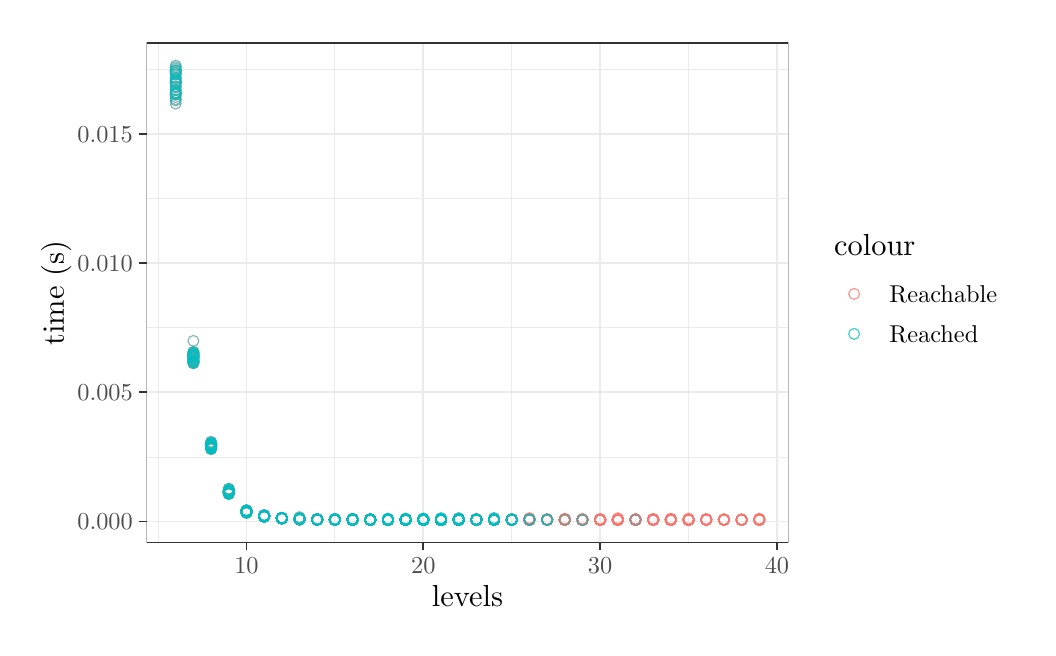
\begin{tikzpicture}[x=1pt,y=1pt]
\definecolor{fillColor}{RGB}{255,255,255}
\path[use as bounding box,fill=fillColor,fill opacity=0.00] (0,0) rectangle (361.35,216.81);
\begin{scope}
\path[clip] (  0.00,  0.00) rectangle (361.35,216.81);
\definecolor{drawColor}{RGB}{255,255,255}
\definecolor{fillColor}{RGB}{255,255,255}

\path[draw=drawColor,line width= 0.6pt,line join=round,line cap=round,fill=fillColor] (  0.00,  0.00) rectangle (361.35,216.81);
\end{scope}
\begin{scope}
\path[clip] ( 42.95, 30.69) rectangle (274.92,211.31);
\definecolor{fillColor}{RGB}{255,255,255}

\path[fill=fillColor] ( 42.95, 30.69) rectangle (274.92,211.31);
\definecolor{drawColor}{gray}{0.92}

\path[draw=drawColor,line width= 0.3pt,line join=round] ( 42.95, 61.69) --
	(274.92, 61.69);

\path[draw=drawColor,line width= 0.3pt,line join=round] ( 42.95,108.41) --
	(274.92,108.41);

\path[draw=drawColor,line width= 0.3pt,line join=round] ( 42.95,155.12) --
	(274.92,155.12);

\path[draw=drawColor,line width= 0.3pt,line join=round] ( 42.95,201.84) --
	(274.92,201.84);

\path[draw=drawColor,line width= 0.3pt,line join=round] ( 47.11, 30.69) --
	( 47.11,211.31);

\path[draw=drawColor,line width= 0.3pt,line join=round] (111.01, 30.69) --
	(111.01,211.31);

\path[draw=drawColor,line width= 0.3pt,line join=round] (174.91, 30.69) --
	(174.91,211.31);

\path[draw=drawColor,line width= 0.3pt,line join=round] (238.81, 30.69) --
	(238.81,211.31);

\path[draw=drawColor,line width= 0.6pt,line join=round] ( 42.95, 38.34) --
	(274.92, 38.34);

\path[draw=drawColor,line width= 0.6pt,line join=round] ( 42.95, 85.05) --
	(274.92, 85.05);

\path[draw=drawColor,line width= 0.6pt,line join=round] ( 42.95,131.77) --
	(274.92,131.77);

\path[draw=drawColor,line width= 0.6pt,line join=round] ( 42.95,178.48) --
	(274.92,178.48);

\path[draw=drawColor,line width= 0.6pt,line join=round] ( 79.06, 30.69) --
	( 79.06,211.31);

\path[draw=drawColor,line width= 0.6pt,line join=round] (142.96, 30.69) --
	(142.96,211.31);

\path[draw=drawColor,line width= 0.6pt,line join=round] (206.86, 30.69) --
	(206.86,211.31);

\path[draw=drawColor,line width= 0.6pt,line join=round] (270.76, 30.69) --
	(270.76,211.31);
\definecolor{drawColor}{RGB}{248,118,109}

\path[draw=drawColor,draw opacity=0.50,line width= 0.4pt,line join=round,line cap=round] ( 79.06, 42.07) circle (  1.96);

\path[draw=drawColor,draw opacity=0.50,line width= 0.4pt,line join=round,line cap=round] ( 79.06, 42.16) circle (  1.96);

\path[draw=drawColor,draw opacity=0.50,line width= 0.4pt,line join=round,line cap=round] ( 79.06, 42.32) circle (  1.96);

\path[draw=drawColor,draw opacity=0.50,line width= 0.4pt,line join=round,line cap=round] ( 79.06, 41.66) circle (  1.96);

\path[draw=drawColor,draw opacity=0.50,line width= 0.4pt,line join=round,line cap=round] ( 79.06, 42.35) circle (  1.96);

\path[draw=drawColor,draw opacity=0.50,line width= 0.4pt,line join=round,line cap=round] ( 79.06, 41.74) circle (  1.96);

\path[draw=drawColor,draw opacity=0.50,line width= 0.4pt,line join=round,line cap=round] ( 79.06, 41.84) circle (  1.96);

\path[draw=drawColor,draw opacity=0.50,line width= 0.4pt,line join=round,line cap=round] ( 79.06, 42.13) circle (  1.96);

\path[draw=drawColor,draw opacity=0.50,line width= 0.4pt,line join=round,line cap=round] ( 79.06, 41.95) circle (  1.96);

\path[draw=drawColor,draw opacity=0.50,line width= 0.4pt,line join=round,line cap=round] ( 79.06, 42.02) circle (  1.96);

\path[draw=drawColor,draw opacity=0.50,line width= 0.4pt,line join=round,line cap=round] ( 79.06, 41.99) circle (  1.96);

\path[draw=drawColor,draw opacity=0.50,line width= 0.4pt,line join=round,line cap=round] ( 79.06, 42.18) circle (  1.96);

\path[draw=drawColor,draw opacity=0.50,line width= 0.4pt,line join=round,line cap=round] ( 79.06, 41.84) circle (  1.96);

\path[draw=drawColor,draw opacity=0.50,line width= 0.4pt,line join=round,line cap=round] ( 79.06, 41.98) circle (  1.96);

\path[draw=drawColor,draw opacity=0.50,line width= 0.4pt,line join=round,line cap=round] ( 79.06, 42.05) circle (  1.96);

\path[draw=drawColor,draw opacity=0.50,line width= 0.4pt,line join=round,line cap=round] ( 79.06, 41.77) circle (  1.96);

\path[draw=drawColor,draw opacity=0.50,line width= 0.4pt,line join=round,line cap=round] ( 79.06, 41.92) circle (  1.96);

\path[draw=drawColor,draw opacity=0.50,line width= 0.4pt,line join=round,line cap=round] ( 79.06, 41.91) circle (  1.96);

\path[draw=drawColor,draw opacity=0.50,line width= 0.4pt,line join=round,line cap=round] ( 79.06, 42.18) circle (  1.96);

\path[draw=drawColor,draw opacity=0.50,line width= 0.4pt,line join=round,line cap=round] ( 79.06, 41.94) circle (  1.96);

\path[draw=drawColor,draw opacity=0.50,line width= 0.4pt,line join=round,line cap=round] ( 79.06, 41.73) circle (  1.96);

\path[draw=drawColor,draw opacity=0.50,line width= 0.4pt,line join=round,line cap=round] ( 79.06, 41.76) circle (  1.96);

\path[draw=drawColor,draw opacity=0.50,line width= 0.4pt,line join=round,line cap=round] ( 79.06, 42.07) circle (  1.96);

\path[draw=drawColor,draw opacity=0.50,line width= 0.4pt,line join=round,line cap=round] ( 79.06, 41.82) circle (  1.96);

\path[draw=drawColor,draw opacity=0.50,line width= 0.4pt,line join=round,line cap=round] ( 79.06, 41.69) circle (  1.96);

\path[draw=drawColor,draw opacity=0.50,line width= 0.4pt,line join=round,line cap=round] ( 79.06, 42.24) circle (  1.96);

\path[draw=drawColor,draw opacity=0.50,line width= 0.4pt,line join=round,line cap=round] ( 79.06, 41.82) circle (  1.96);

\path[draw=drawColor,draw opacity=0.50,line width= 0.4pt,line join=round,line cap=round] ( 79.06, 41.95) circle (  1.96);

\path[draw=drawColor,draw opacity=0.50,line width= 0.4pt,line join=round,line cap=round] ( 79.06, 42.24) circle (  1.96);

\path[draw=drawColor,draw opacity=0.50,line width= 0.4pt,line join=round,line cap=round] ( 79.06, 41.75) circle (  1.96);

\path[draw=drawColor,draw opacity=0.50,line width= 0.4pt,line join=round,line cap=round] ( 79.06, 42.15) circle (  1.96);

\path[draw=drawColor,draw opacity=0.50,line width= 0.4pt,line join=round,line cap=round] ( 79.06, 42.01) circle (  1.96);

\path[draw=drawColor,draw opacity=0.50,line width= 0.4pt,line join=round,line cap=round] ( 79.06, 42.15) circle (  1.96);

\path[draw=drawColor,draw opacity=0.50,line width= 0.4pt,line join=round,line cap=round] ( 79.06, 41.90) circle (  1.96);

\path[draw=drawColor,draw opacity=0.50,line width= 0.4pt,line join=round,line cap=round] ( 85.45, 40.15) circle (  1.96);

\path[draw=drawColor,draw opacity=0.50,line width= 0.4pt,line join=round,line cap=round] ( 85.45, 40.30) circle (  1.96);

\path[draw=drawColor,draw opacity=0.50,line width= 0.4pt,line join=round,line cap=round] ( 85.45, 40.19) circle (  1.96);

\path[draw=drawColor,draw opacity=0.50,line width= 0.4pt,line join=round,line cap=round] ( 85.45, 40.32) circle (  1.96);

\path[draw=drawColor,draw opacity=0.50,line width= 0.4pt,line join=round,line cap=round] ( 85.45, 40.42) circle (  1.96);

\path[draw=drawColor,draw opacity=0.50,line width= 0.4pt,line join=round,line cap=round] ( 85.45, 40.11) circle (  1.96);

\path[draw=drawColor,draw opacity=0.50,line width= 0.4pt,line join=round,line cap=round] ( 85.45, 40.28) circle (  1.96);

\path[draw=drawColor,draw opacity=0.50,line width= 0.4pt,line join=round,line cap=round] ( 85.45, 40.36) circle (  1.96);

\path[draw=drawColor,draw opacity=0.50,line width= 0.4pt,line join=round,line cap=round] ( 85.45, 40.05) circle (  1.96);

\path[draw=drawColor,draw opacity=0.50,line width= 0.4pt,line join=round,line cap=round] ( 85.45, 40.26) circle (  1.96);

\path[draw=drawColor,draw opacity=0.50,line width= 0.4pt,line join=round,line cap=round] ( 85.45, 40.42) circle (  1.96);

\path[draw=drawColor,draw opacity=0.50,line width= 0.4pt,line join=round,line cap=round] ( 85.45, 40.19) circle (  1.96);

\path[draw=drawColor,draw opacity=0.50,line width= 0.4pt,line join=round,line cap=round] ( 85.45, 40.33) circle (  1.96);

\path[draw=drawColor,draw opacity=0.50,line width= 0.4pt,line join=round,line cap=round] ( 85.45, 40.19) circle (  1.96);

\path[draw=drawColor,draw opacity=0.50,line width= 0.4pt,line join=round,line cap=round] ( 85.45, 40.34) circle (  1.96);

\path[draw=drawColor,draw opacity=0.50,line width= 0.4pt,line join=round,line cap=round] ( 85.45, 40.73) circle (  1.96);

\path[draw=drawColor,draw opacity=0.50,line width= 0.4pt,line join=round,line cap=round] ( 85.45, 40.05) circle (  1.96);

\path[draw=drawColor,draw opacity=0.50,line width= 0.4pt,line join=round,line cap=round] ( 85.45, 40.34) circle (  1.96);

\path[draw=drawColor,draw opacity=0.50,line width= 0.4pt,line join=round,line cap=round] ( 85.45, 40.22) circle (  1.96);

\path[draw=drawColor,draw opacity=0.50,line width= 0.4pt,line join=round,line cap=round] ( 85.45, 40.29) circle (  1.96);

\path[draw=drawColor,draw opacity=0.50,line width= 0.4pt,line join=round,line cap=round] ( 85.45, 40.21) circle (  1.96);

\path[draw=drawColor,draw opacity=0.50,line width= 0.4pt,line join=round,line cap=round] ( 85.45, 40.21) circle (  1.96);

\path[draw=drawColor,draw opacity=0.50,line width= 0.4pt,line join=round,line cap=round] ( 85.45, 40.11) circle (  1.96);

\path[draw=drawColor,draw opacity=0.50,line width= 0.4pt,line join=round,line cap=round] ( 85.45, 40.63) circle (  1.96);

\path[draw=drawColor,draw opacity=0.50,line width= 0.4pt,line join=round,line cap=round] ( 85.45, 40.17) circle (  1.96);

\path[draw=drawColor,draw opacity=0.50,line width= 0.4pt,line join=round,line cap=round] ( 85.45, 40.27) circle (  1.96);

\path[draw=drawColor,draw opacity=0.50,line width= 0.4pt,line join=round,line cap=round] ( 85.45, 40.31) circle (  1.96);

\path[draw=drawColor,draw opacity=0.50,line width= 0.4pt,line join=round,line cap=round] ( 85.45, 40.51) circle (  1.96);

\path[draw=drawColor,draw opacity=0.50,line width= 0.4pt,line join=round,line cap=round] ( 85.45, 40.30) circle (  1.96);

\path[draw=drawColor,draw opacity=0.50,line width= 0.4pt,line join=round,line cap=round] ( 85.45, 40.32) circle (  1.96);

\path[draw=drawColor,draw opacity=0.50,line width= 0.4pt,line join=round,line cap=round] ( 85.45, 40.22) circle (  1.96);

\path[draw=drawColor,draw opacity=0.50,line width= 0.4pt,line join=round,line cap=round] ( 85.45, 40.21) circle (  1.96);

\path[draw=drawColor,draw opacity=0.50,line width= 0.4pt,line join=round,line cap=round] ( 85.45, 40.36) circle (  1.96);

\path[draw=drawColor,draw opacity=0.50,line width= 0.4pt,line join=round,line cap=round] ( 91.84, 39.52) circle (  1.96);

\path[draw=drawColor,draw opacity=0.50,line width= 0.4pt,line join=round,line cap=round] ( 91.84, 39.63) circle (  1.96);

\path[draw=drawColor,draw opacity=0.50,line width= 0.4pt,line join=round,line cap=round] ( 91.84, 39.51) circle (  1.96);

\path[draw=drawColor,draw opacity=0.50,line width= 0.4pt,line join=round,line cap=round] ( 91.84, 39.48) circle (  1.96);

\path[draw=drawColor,draw opacity=0.50,line width= 0.4pt,line join=round,line cap=round] ( 91.84, 39.55) circle (  1.96);

\path[draw=drawColor,draw opacity=0.50,line width= 0.4pt,line join=round,line cap=round] ( 91.84, 39.44) circle (  1.96);

\path[draw=drawColor,draw opacity=0.50,line width= 0.4pt,line join=round,line cap=round] ( 91.84, 39.55) circle (  1.96);

\path[draw=drawColor,draw opacity=0.50,line width= 0.4pt,line join=round,line cap=round] ( 91.84, 39.43) circle (  1.96);

\path[draw=drawColor,draw opacity=0.50,line width= 0.4pt,line join=round,line cap=round] ( 91.84, 39.51) circle (  1.96);

\path[draw=drawColor,draw opacity=0.50,line width= 0.4pt,line join=round,line cap=round] ( 91.84, 39.68) circle (  1.96);

\path[draw=drawColor,draw opacity=0.50,line width= 0.4pt,line join=round,line cap=round] ( 91.84, 39.49) circle (  1.96);

\path[draw=drawColor,draw opacity=0.50,line width= 0.4pt,line join=round,line cap=round] ( 91.84, 39.56) circle (  1.96);

\path[draw=drawColor,draw opacity=0.50,line width= 0.4pt,line join=round,line cap=round] ( 91.84, 39.60) circle (  1.96);

\path[draw=drawColor,draw opacity=0.50,line width= 0.4pt,line join=round,line cap=round] ( 91.84, 39.56) circle (  1.96);

\path[draw=drawColor,draw opacity=0.50,line width= 0.4pt,line join=round,line cap=round] ( 91.84, 39.52) circle (  1.96);

\path[draw=drawColor,draw opacity=0.50,line width= 0.4pt,line join=round,line cap=round] ( 91.84, 39.58) circle (  1.96);

\path[draw=drawColor,draw opacity=0.50,line width= 0.4pt,line join=round,line cap=round] ( 91.84, 39.58) circle (  1.96);

\path[draw=drawColor,draw opacity=0.50,line width= 0.4pt,line join=round,line cap=round] ( 91.84, 39.53) circle (  1.96);

\path[draw=drawColor,draw opacity=0.50,line width= 0.4pt,line join=round,line cap=round] ( 91.84, 39.55) circle (  1.96);

\path[draw=drawColor,draw opacity=0.50,line width= 0.4pt,line join=round,line cap=round] ( 91.84, 39.49) circle (  1.96);

\path[draw=drawColor,draw opacity=0.50,line width= 0.4pt,line join=round,line cap=round] ( 91.84, 39.44) circle (  1.96);

\path[draw=drawColor,draw opacity=0.50,line width= 0.4pt,line join=round,line cap=round] ( 91.84, 39.57) circle (  1.96);

\path[draw=drawColor,draw opacity=0.50,line width= 0.4pt,line join=round,line cap=round] ( 91.84, 39.54) circle (  1.96);

\path[draw=drawColor,draw opacity=0.50,line width= 0.4pt,line join=round,line cap=round] ( 91.84, 39.52) circle (  1.96);

\path[draw=drawColor,draw opacity=0.50,line width= 0.4pt,line join=round,line cap=round] ( 91.84, 39.53) circle (  1.96);

\path[draw=drawColor,draw opacity=0.50,line width= 0.4pt,line join=round,line cap=round] ( 91.84, 39.52) circle (  1.96);

\path[draw=drawColor,draw opacity=0.50,line width= 0.4pt,line join=round,line cap=round] ( 91.84, 39.51) circle (  1.96);

\path[draw=drawColor,draw opacity=0.50,line width= 0.4pt,line join=round,line cap=round] ( 91.84, 39.53) circle (  1.96);

\path[draw=drawColor,draw opacity=0.50,line width= 0.4pt,line join=round,line cap=round] ( 91.84, 39.55) circle (  1.96);

\path[draw=drawColor,draw opacity=0.50,line width= 0.4pt,line join=round,line cap=round] ( 91.84, 39.46) circle (  1.96);

\path[draw=drawColor,draw opacity=0.50,line width= 0.4pt,line join=round,line cap=round] ( 91.84, 39.52) circle (  1.96);

\path[draw=drawColor,draw opacity=0.50,line width= 0.4pt,line join=round,line cap=round] ( 91.84, 39.56) circle (  1.96);

\path[draw=drawColor,draw opacity=0.50,line width= 0.4pt,line join=round,line cap=round] ( 91.84, 39.53) circle (  1.96);

\path[draw=drawColor,draw opacity=0.50,line width= 0.4pt,line join=round,line cap=round] ( 98.23, 39.18) circle (  1.96);

\path[draw=drawColor,draw opacity=0.50,line width= 0.4pt,line join=round,line cap=round] ( 98.23, 39.19) circle (  1.96);

\path[draw=drawColor,draw opacity=0.50,line width= 0.4pt,line join=round,line cap=round] ( 98.23, 39.25) circle (  1.96);

\path[draw=drawColor,draw opacity=0.50,line width= 0.4pt,line join=round,line cap=round] ( 98.23, 39.19) circle (  1.96);

\path[draw=drawColor,draw opacity=0.50,line width= 0.4pt,line join=round,line cap=round] ( 98.23, 39.12) circle (  1.96);

\path[draw=drawColor,draw opacity=0.50,line width= 0.4pt,line join=round,line cap=round] ( 98.23, 39.61) circle (  1.96);

\path[draw=drawColor,draw opacity=0.50,line width= 0.4pt,line join=round,line cap=round] ( 98.23, 39.21) circle (  1.96);

\path[draw=drawColor,draw opacity=0.50,line width= 0.4pt,line join=round,line cap=round] ( 98.23, 39.20) circle (  1.96);

\path[draw=drawColor,draw opacity=0.50,line width= 0.4pt,line join=round,line cap=round] ( 98.23, 39.27) circle (  1.96);

\path[draw=drawColor,draw opacity=0.50,line width= 0.4pt,line join=round,line cap=round] ( 98.23, 39.13) circle (  1.96);

\path[draw=drawColor,draw opacity=0.50,line width= 0.4pt,line join=round,line cap=round] ( 98.23, 39.17) circle (  1.96);

\path[draw=drawColor,draw opacity=0.50,line width= 0.4pt,line join=round,line cap=round] ( 98.23, 39.25) circle (  1.96);

\path[draw=drawColor,draw opacity=0.50,line width= 0.4pt,line join=round,line cap=round] ( 98.23, 39.22) circle (  1.96);

\path[draw=drawColor,draw opacity=0.50,line width= 0.4pt,line join=round,line cap=round] ( 98.23, 39.25) circle (  1.96);

\path[draw=drawColor,draw opacity=0.50,line width= 0.4pt,line join=round,line cap=round] ( 98.23, 39.19) circle (  1.96);

\path[draw=drawColor,draw opacity=0.50,line width= 0.4pt,line join=round,line cap=round] ( 98.23, 39.23) circle (  1.96);

\path[draw=drawColor,draw opacity=0.50,line width= 0.4pt,line join=round,line cap=round] ( 98.23, 39.20) circle (  1.96);

\path[draw=drawColor,draw opacity=0.50,line width= 0.4pt,line join=round,line cap=round] ( 98.23, 39.20) circle (  1.96);

\path[draw=drawColor,draw opacity=0.50,line width= 0.4pt,line join=round,line cap=round] ( 98.23, 39.12) circle (  1.96);

\path[draw=drawColor,draw opacity=0.50,line width= 0.4pt,line join=round,line cap=round] ( 98.23, 39.30) circle (  1.96);

\path[draw=drawColor,draw opacity=0.50,line width= 0.4pt,line join=round,line cap=round] ( 98.23, 39.19) circle (  1.96);

\path[draw=drawColor,draw opacity=0.50,line width= 0.4pt,line join=round,line cap=round] ( 98.23, 39.19) circle (  1.96);

\path[draw=drawColor,draw opacity=0.50,line width= 0.4pt,line join=round,line cap=round] ( 98.23, 39.23) circle (  1.96);

\path[draw=drawColor,draw opacity=0.50,line width= 0.4pt,line join=round,line cap=round] ( 98.23, 39.15) circle (  1.96);

\path[draw=drawColor,draw opacity=0.50,line width= 0.4pt,line join=round,line cap=round] ( 98.23, 39.22) circle (  1.96);

\path[draw=drawColor,draw opacity=0.50,line width= 0.4pt,line join=round,line cap=round] ( 98.23, 39.19) circle (  1.96);

\path[draw=drawColor,draw opacity=0.50,line width= 0.4pt,line join=round,line cap=round] ( 98.23, 39.19) circle (  1.96);

\path[draw=drawColor,draw opacity=0.50,line width= 0.4pt,line join=round,line cap=round] ( 98.23, 39.34) circle (  1.96);

\path[draw=drawColor,draw opacity=0.50,line width= 0.4pt,line join=round,line cap=round] ( 98.23, 39.19) circle (  1.96);

\path[draw=drawColor,draw opacity=0.50,line width= 0.4pt,line join=round,line cap=round] ( 98.23, 39.19) circle (  1.96);

\path[draw=drawColor,draw opacity=0.50,line width= 0.4pt,line join=round,line cap=round] ( 98.23, 39.15) circle (  1.96);

\path[draw=drawColor,draw opacity=0.50,line width= 0.4pt,line join=round,line cap=round] ( 98.23, 39.18) circle (  1.96);

\path[draw=drawColor,draw opacity=0.50,line width= 0.4pt,line join=round,line cap=round] ( 98.23, 39.27) circle (  1.96);

\path[draw=drawColor,draw opacity=0.50,line width= 0.4pt,line join=round,line cap=round] (104.62, 39.06) circle (  1.96);

\path[draw=drawColor,draw opacity=0.50,line width= 0.4pt,line join=round,line cap=round] (104.62, 39.11) circle (  1.96);

\path[draw=drawColor,draw opacity=0.50,line width= 0.4pt,line join=round,line cap=round] (104.62, 39.09) circle (  1.96);

\path[draw=drawColor,draw opacity=0.50,line width= 0.4pt,line join=round,line cap=round] (104.62, 39.14) circle (  1.96);

\path[draw=drawColor,draw opacity=0.50,line width= 0.4pt,line join=round,line cap=round] (104.62, 39.10) circle (  1.96);

\path[draw=drawColor,draw opacity=0.50,line width= 0.4pt,line join=round,line cap=round] (104.62, 39.05) circle (  1.96);

\path[draw=drawColor,draw opacity=0.50,line width= 0.4pt,line join=round,line cap=round] (104.62, 39.11) circle (  1.96);

\path[draw=drawColor,draw opacity=0.50,line width= 0.4pt,line join=round,line cap=round] (104.62, 39.06) circle (  1.96);

\path[draw=drawColor,draw opacity=0.50,line width= 0.4pt,line join=round,line cap=round] (104.62, 39.08) circle (  1.96);

\path[draw=drawColor,draw opacity=0.50,line width= 0.4pt,line join=round,line cap=round] (104.62, 39.03) circle (  1.96);

\path[draw=drawColor,draw opacity=0.50,line width= 0.4pt,line join=round,line cap=round] (104.62, 39.28) circle (  1.96);

\path[draw=drawColor,draw opacity=0.50,line width= 0.4pt,line join=round,line cap=round] (104.62, 39.06) circle (  1.96);

\path[draw=drawColor,draw opacity=0.50,line width= 0.4pt,line join=round,line cap=round] (104.62, 39.02) circle (  1.96);

\path[draw=drawColor,draw opacity=0.50,line width= 0.4pt,line join=round,line cap=round] (104.62, 39.12) circle (  1.96);

\path[draw=drawColor,draw opacity=0.50,line width= 0.4pt,line join=round,line cap=round] (104.62, 39.03) circle (  1.96);

\path[draw=drawColor,draw opacity=0.50,line width= 0.4pt,line join=round,line cap=round] (104.62, 39.03) circle (  1.96);

\path[draw=drawColor,draw opacity=0.50,line width= 0.4pt,line join=round,line cap=round] (104.62, 39.18) circle (  1.96);

\path[draw=drawColor,draw opacity=0.50,line width= 0.4pt,line join=round,line cap=round] (104.62, 39.06) circle (  1.96);

\path[draw=drawColor,draw opacity=0.50,line width= 0.4pt,line join=round,line cap=round] (104.62, 39.05) circle (  1.96);

\path[draw=drawColor,draw opacity=0.50,line width= 0.4pt,line join=round,line cap=round] (104.62, 39.07) circle (  1.96);

\path[draw=drawColor,draw opacity=0.50,line width= 0.4pt,line join=round,line cap=round] (104.62, 39.01) circle (  1.96);

\path[draw=drawColor,draw opacity=0.50,line width= 0.4pt,line join=round,line cap=round] (104.62, 39.04) circle (  1.96);

\path[draw=drawColor,draw opacity=0.50,line width= 0.4pt,line join=round,line cap=round] (104.62, 39.08) circle (  1.96);

\path[draw=drawColor,draw opacity=0.50,line width= 0.4pt,line join=round,line cap=round] (104.62, 39.06) circle (  1.96);

\path[draw=drawColor,draw opacity=0.50,line width= 0.4pt,line join=round,line cap=round] (104.62, 38.97) circle (  1.96);

\path[draw=drawColor,draw opacity=0.50,line width= 0.4pt,line join=round,line cap=round] (104.62, 39.08) circle (  1.96);

\path[draw=drawColor,draw opacity=0.50,line width= 0.4pt,line join=round,line cap=round] (104.62, 39.16) circle (  1.96);

\path[draw=drawColor,draw opacity=0.50,line width= 0.4pt,line join=round,line cap=round] (104.62, 39.11) circle (  1.96);

\path[draw=drawColor,draw opacity=0.50,line width= 0.4pt,line join=round,line cap=round] (104.62, 39.06) circle (  1.96);

\path[draw=drawColor,draw opacity=0.50,line width= 0.4pt,line join=round,line cap=round] (104.62, 39.09) circle (  1.96);

\path[draw=drawColor,draw opacity=0.50,line width= 0.4pt,line join=round,line cap=round] (104.62, 39.24) circle (  1.96);

\path[draw=drawColor,draw opacity=0.50,line width= 0.4pt,line join=round,line cap=round] (104.62, 39.09) circle (  1.96);

\path[draw=drawColor,draw opacity=0.50,line width= 0.4pt,line join=round,line cap=round] (104.62, 39.02) circle (  1.96);

\path[draw=drawColor,draw opacity=0.50,line width= 0.4pt,line join=round,line cap=round] (111.01, 39.03) circle (  1.96);

\path[draw=drawColor,draw opacity=0.50,line width= 0.4pt,line join=round,line cap=round] (111.01, 39.02) circle (  1.96);

\path[draw=drawColor,draw opacity=0.50,line width= 0.4pt,line join=round,line cap=round] (111.01, 39.08) circle (  1.96);

\path[draw=drawColor,draw opacity=0.50,line width= 0.4pt,line join=round,line cap=round] (111.01, 39.28) circle (  1.96);

\path[draw=drawColor,draw opacity=0.50,line width= 0.4pt,line join=round,line cap=round] (111.01, 39.01) circle (  1.96);

\path[draw=drawColor,draw opacity=0.50,line width= 0.4pt,line join=round,line cap=round] (111.01, 39.04) circle (  1.96);

\path[draw=drawColor,draw opacity=0.50,line width= 0.4pt,line join=round,line cap=round] (111.01, 39.02) circle (  1.96);

\path[draw=drawColor,draw opacity=0.50,line width= 0.4pt,line join=round,line cap=round] (111.01, 39.14) circle (  1.96);

\path[draw=drawColor,draw opacity=0.50,line width= 0.4pt,line join=round,line cap=round] (111.01, 39.01) circle (  1.96);

\path[draw=drawColor,draw opacity=0.50,line width= 0.4pt,line join=round,line cap=round] (111.01, 39.01) circle (  1.96);

\path[draw=drawColor,draw opacity=0.50,line width= 0.4pt,line join=round,line cap=round] (111.01, 39.02) circle (  1.96);

\path[draw=drawColor,draw opacity=0.50,line width= 0.4pt,line join=round,line cap=round] (111.01, 39.02) circle (  1.96);

\path[draw=drawColor,draw opacity=0.50,line width= 0.4pt,line join=round,line cap=round] (111.01, 39.01) circle (  1.96);

\path[draw=drawColor,draw opacity=0.50,line width= 0.4pt,line join=round,line cap=round] (111.01, 39.05) circle (  1.96);

\path[draw=drawColor,draw opacity=0.50,line width= 0.4pt,line join=round,line cap=round] (111.01, 39.03) circle (  1.96);

\path[draw=drawColor,draw opacity=0.50,line width= 0.4pt,line join=round,line cap=round] (111.01, 38.95) circle (  1.96);

\path[draw=drawColor,draw opacity=0.50,line width= 0.4pt,line join=round,line cap=round] (111.01, 39.32) circle (  1.96);

\path[draw=drawColor,draw opacity=0.50,line width= 0.4pt,line join=round,line cap=round] (111.01, 39.04) circle (  1.96);

\path[draw=drawColor,draw opacity=0.50,line width= 0.4pt,line join=round,line cap=round] (111.01, 39.09) circle (  1.96);

\path[draw=drawColor,draw opacity=0.50,line width= 0.4pt,line join=round,line cap=round] (111.01, 39.04) circle (  1.96);

\path[draw=drawColor,draw opacity=0.50,line width= 0.4pt,line join=round,line cap=round] (111.01, 39.02) circle (  1.96);

\path[draw=drawColor,draw opacity=0.50,line width= 0.4pt,line join=round,line cap=round] (111.01, 38.95) circle (  1.96);

\path[draw=drawColor,draw opacity=0.50,line width= 0.4pt,line join=round,line cap=round] (111.01, 39.05) circle (  1.96);

\path[draw=drawColor,draw opacity=0.50,line width= 0.4pt,line join=round,line cap=round] (111.01, 39.00) circle (  1.96);

\path[draw=drawColor,draw opacity=0.50,line width= 0.4pt,line join=round,line cap=round] (111.01, 38.99) circle (  1.96);

\path[draw=drawColor,draw opacity=0.50,line width= 0.4pt,line join=round,line cap=round] (111.01, 39.02) circle (  1.96);

\path[draw=drawColor,draw opacity=0.50,line width= 0.4pt,line join=round,line cap=round] (111.01, 39.00) circle (  1.96);

\path[draw=drawColor,draw opacity=0.50,line width= 0.4pt,line join=round,line cap=round] (111.01, 39.01) circle (  1.96);

\path[draw=drawColor,draw opacity=0.50,line width= 0.4pt,line join=round,line cap=round] (111.01, 38.99) circle (  1.96);

\path[draw=drawColor,draw opacity=0.50,line width= 0.4pt,line join=round,line cap=round] (111.01, 39.01) circle (  1.96);

\path[draw=drawColor,draw opacity=0.50,line width= 0.4pt,line join=round,line cap=round] (111.01, 39.10) circle (  1.96);

\path[draw=drawColor,draw opacity=0.50,line width= 0.4pt,line join=round,line cap=round] (111.01, 39.08) circle (  1.96);

\path[draw=drawColor,draw opacity=0.50,line width= 0.4pt,line join=round,line cap=round] (111.01, 38.99) circle (  1.96);

\path[draw=drawColor,draw opacity=0.50,line width= 0.4pt,line join=round,line cap=round] (117.40, 38.93) circle (  1.96);

\path[draw=drawColor,draw opacity=0.50,line width= 0.4pt,line join=round,line cap=round] (117.40, 39.03) circle (  1.96);

\path[draw=drawColor,draw opacity=0.50,line width= 0.4pt,line join=round,line cap=round] (117.40, 39.01) circle (  1.96);

\path[draw=drawColor,draw opacity=0.50,line width= 0.4pt,line join=round,line cap=round] (117.40, 39.33) circle (  1.96);

\path[draw=drawColor,draw opacity=0.50,line width= 0.4pt,line join=round,line cap=round] (117.40, 39.03) circle (  1.96);

\path[draw=drawColor,draw opacity=0.50,line width= 0.4pt,line join=round,line cap=round] (117.40, 38.94) circle (  1.96);

\path[draw=drawColor,draw opacity=0.50,line width= 0.4pt,line join=round,line cap=round] (117.40, 38.98) circle (  1.96);

\path[draw=drawColor,draw opacity=0.50,line width= 0.4pt,line join=round,line cap=round] (117.40, 39.00) circle (  1.96);

\path[draw=drawColor,draw opacity=0.50,line width= 0.4pt,line join=round,line cap=round] (117.40, 39.06) circle (  1.96);

\path[draw=drawColor,draw opacity=0.50,line width= 0.4pt,line join=round,line cap=round] (117.40, 39.21) circle (  1.96);

\path[draw=drawColor,draw opacity=0.50,line width= 0.4pt,line join=round,line cap=round] (117.40, 39.02) circle (  1.96);

\path[draw=drawColor,draw opacity=0.50,line width= 0.4pt,line join=round,line cap=round] (117.40, 39.00) circle (  1.96);

\path[draw=drawColor,draw opacity=0.50,line width= 0.4pt,line join=round,line cap=round] (117.40, 39.05) circle (  1.96);

\path[draw=drawColor,draw opacity=0.50,line width= 0.4pt,line join=round,line cap=round] (117.40, 39.01) circle (  1.96);

\path[draw=drawColor,draw opacity=0.50,line width= 0.4pt,line join=round,line cap=round] (117.40, 39.00) circle (  1.96);

\path[draw=drawColor,draw opacity=0.50,line width= 0.4pt,line join=round,line cap=round] (117.40, 39.03) circle (  1.96);

\path[draw=drawColor,draw opacity=0.50,line width= 0.4pt,line join=round,line cap=round] (117.40, 38.98) circle (  1.96);

\path[draw=drawColor,draw opacity=0.50,line width= 0.4pt,line join=round,line cap=round] (117.40, 39.06) circle (  1.96);

\path[draw=drawColor,draw opacity=0.50,line width= 0.4pt,line join=round,line cap=round] (117.40, 38.96) circle (  1.96);

\path[draw=drawColor,draw opacity=0.50,line width= 0.4pt,line join=round,line cap=round] (117.40, 39.04) circle (  1.96);

\path[draw=drawColor,draw opacity=0.50,line width= 0.4pt,line join=round,line cap=round] (117.40, 39.05) circle (  1.96);

\path[draw=drawColor,draw opacity=0.50,line width= 0.4pt,line join=round,line cap=round] (117.40, 39.05) circle (  1.96);

\path[draw=drawColor,draw opacity=0.50,line width= 0.4pt,line join=round,line cap=round] (117.40, 38.98) circle (  1.96);

\path[draw=drawColor,draw opacity=0.50,line width= 0.4pt,line join=round,line cap=round] (117.40, 38.96) circle (  1.96);

\path[draw=drawColor,draw opacity=0.50,line width= 0.4pt,line join=round,line cap=round] (117.40, 38.98) circle (  1.96);

\path[draw=drawColor,draw opacity=0.50,line width= 0.4pt,line join=round,line cap=round] (117.40, 39.07) circle (  1.96);

\path[draw=drawColor,draw opacity=0.50,line width= 0.4pt,line join=round,line cap=round] (117.40, 39.04) circle (  1.96);

\path[draw=drawColor,draw opacity=0.50,line width= 0.4pt,line join=round,line cap=round] (117.40, 39.03) circle (  1.96);

\path[draw=drawColor,draw opacity=0.50,line width= 0.4pt,line join=round,line cap=round] (117.40, 38.99) circle (  1.96);

\path[draw=drawColor,draw opacity=0.50,line width= 0.4pt,line join=round,line cap=round] (117.40, 39.00) circle (  1.96);

\path[draw=drawColor,draw opacity=0.50,line width= 0.4pt,line join=round,line cap=round] (117.40, 39.04) circle (  1.96);

\path[draw=drawColor,draw opacity=0.50,line width= 0.4pt,line join=round,line cap=round] (117.40, 39.06) circle (  1.96);

\path[draw=drawColor,draw opacity=0.50,line width= 0.4pt,line join=round,line cap=round] (117.40, 38.98) circle (  1.96);

\path[draw=drawColor,draw opacity=0.50,line width= 0.4pt,line join=round,line cap=round] (123.79, 38.99) circle (  1.96);

\path[draw=drawColor,draw opacity=0.50,line width= 0.4pt,line join=round,line cap=round] (123.79, 39.03) circle (  1.96);

\path[draw=drawColor,draw opacity=0.50,line width= 0.4pt,line join=round,line cap=round] (123.79, 39.02) circle (  1.96);

\path[draw=drawColor,draw opacity=0.50,line width= 0.4pt,line join=round,line cap=round] (123.79, 39.03) circle (  1.96);

\path[draw=drawColor,draw opacity=0.50,line width= 0.4pt,line join=round,line cap=round] (123.79, 39.02) circle (  1.96);

\path[draw=drawColor,draw opacity=0.50,line width= 0.4pt,line join=round,line cap=round] (123.79, 38.94) circle (  1.96);

\path[draw=drawColor,draw opacity=0.50,line width= 0.4pt,line join=round,line cap=round] (123.79, 39.05) circle (  1.96);

\path[draw=drawColor,draw opacity=0.50,line width= 0.4pt,line join=round,line cap=round] (123.79, 39.00) circle (  1.96);

\path[draw=drawColor,draw opacity=0.50,line width= 0.4pt,line join=round,line cap=round] (123.79, 39.00) circle (  1.96);

\path[draw=drawColor,draw opacity=0.50,line width= 0.4pt,line join=round,line cap=round] (123.79, 39.01) circle (  1.96);

\path[draw=drawColor,draw opacity=0.50,line width= 0.4pt,line join=round,line cap=round] (123.79, 39.03) circle (  1.96);

\path[draw=drawColor,draw opacity=0.50,line width= 0.4pt,line join=round,line cap=round] (123.79, 38.92) circle (  1.96);

\path[draw=drawColor,draw opacity=0.50,line width= 0.4pt,line join=round,line cap=round] (123.79, 39.05) circle (  1.96);

\path[draw=drawColor,draw opacity=0.50,line width= 0.4pt,line join=round,line cap=round] (123.79, 38.98) circle (  1.96);

\path[draw=drawColor,draw opacity=0.50,line width= 0.4pt,line join=round,line cap=round] (123.79, 39.00) circle (  1.96);

\path[draw=drawColor,draw opacity=0.50,line width= 0.4pt,line join=round,line cap=round] (123.79, 39.01) circle (  1.96);

\path[draw=drawColor,draw opacity=0.50,line width= 0.4pt,line join=round,line cap=round] (123.79, 39.03) circle (  1.96);

\path[draw=drawColor,draw opacity=0.50,line width= 0.4pt,line join=round,line cap=round] (123.79, 38.94) circle (  1.96);

\path[draw=drawColor,draw opacity=0.50,line width= 0.4pt,line join=round,line cap=round] (123.79, 38.92) circle (  1.96);

\path[draw=drawColor,draw opacity=0.50,line width= 0.4pt,line join=round,line cap=round] (123.79, 39.11) circle (  1.96);

\path[draw=drawColor,draw opacity=0.50,line width= 0.4pt,line join=round,line cap=round] (123.79, 39.05) circle (  1.96);

\path[draw=drawColor,draw opacity=0.50,line width= 0.4pt,line join=round,line cap=round] (123.79, 38.96) circle (  1.96);

\path[draw=drawColor,draw opacity=0.50,line width= 0.4pt,line join=round,line cap=round] (123.79, 38.97) circle (  1.96);

\path[draw=drawColor,draw opacity=0.50,line width= 0.4pt,line join=round,line cap=round] (123.79, 39.34) circle (  1.96);

\path[draw=drawColor,draw opacity=0.50,line width= 0.4pt,line join=round,line cap=round] (123.79, 39.05) circle (  1.96);

\path[draw=drawColor,draw opacity=0.50,line width= 0.4pt,line join=round,line cap=round] (123.79, 38.95) circle (  1.96);

\path[draw=drawColor,draw opacity=0.50,line width= 0.4pt,line join=round,line cap=round] (123.79, 38.98) circle (  1.96);

\path[draw=drawColor,draw opacity=0.50,line width= 0.4pt,line join=round,line cap=round] (123.79, 39.02) circle (  1.96);

\path[draw=drawColor,draw opacity=0.50,line width= 0.4pt,line join=round,line cap=round] (123.79, 39.00) circle (  1.96);

\path[draw=drawColor,draw opacity=0.50,line width= 0.4pt,line join=round,line cap=round] (123.79, 38.98) circle (  1.96);

\path[draw=drawColor,draw opacity=0.50,line width= 0.4pt,line join=round,line cap=round] (123.79, 39.01) circle (  1.96);

\path[draw=drawColor,draw opacity=0.50,line width= 0.4pt,line join=round,line cap=round] (123.79, 39.00) circle (  1.96);

\path[draw=drawColor,draw opacity=0.50,line width= 0.4pt,line join=round,line cap=round] (123.79, 39.02) circle (  1.96);

\path[draw=drawColor,draw opacity=0.50,line width= 0.4pt,line join=round,line cap=round] (130.18, 39.06) circle (  1.96);

\path[draw=drawColor,draw opacity=0.50,line width= 0.4pt,line join=round,line cap=round] (130.18, 39.07) circle (  1.96);

\path[draw=drawColor,draw opacity=0.50,line width= 0.4pt,line join=round,line cap=round] (130.18, 38.99) circle (  1.96);

\path[draw=drawColor,draw opacity=0.50,line width= 0.4pt,line join=round,line cap=round] (130.18, 38.91) circle (  1.96);

\path[draw=drawColor,draw opacity=0.50,line width= 0.4pt,line join=round,line cap=round] (130.18, 39.00) circle (  1.96);

\path[draw=drawColor,draw opacity=0.50,line width= 0.4pt,line join=round,line cap=round] (130.18, 38.94) circle (  1.96);

\path[draw=drawColor,draw opacity=0.50,line width= 0.4pt,line join=round,line cap=round] (130.18, 39.07) circle (  1.96);

\path[draw=drawColor,draw opacity=0.50,line width= 0.4pt,line join=round,line cap=round] (130.18, 38.97) circle (  1.96);

\path[draw=drawColor,draw opacity=0.50,line width= 0.4pt,line join=round,line cap=round] (130.18, 39.05) circle (  1.96);

\path[draw=drawColor,draw opacity=0.50,line width= 0.4pt,line join=round,line cap=round] (130.18, 39.04) circle (  1.96);

\path[draw=drawColor,draw opacity=0.50,line width= 0.4pt,line join=round,line cap=round] (130.18, 38.98) circle (  1.96);

\path[draw=drawColor,draw opacity=0.50,line width= 0.4pt,line join=round,line cap=round] (130.18, 38.95) circle (  1.96);

\path[draw=drawColor,draw opacity=0.50,line width= 0.4pt,line join=round,line cap=round] (130.18, 38.98) circle (  1.96);

\path[draw=drawColor,draw opacity=0.50,line width= 0.4pt,line join=round,line cap=round] (130.18, 39.00) circle (  1.96);

\path[draw=drawColor,draw opacity=0.50,line width= 0.4pt,line join=round,line cap=round] (130.18, 39.34) circle (  1.96);

\path[draw=drawColor,draw opacity=0.50,line width= 0.4pt,line join=round,line cap=round] (130.18, 39.01) circle (  1.96);

\path[draw=drawColor,draw opacity=0.50,line width= 0.4pt,line join=round,line cap=round] (130.18, 39.02) circle (  1.96);

\path[draw=drawColor,draw opacity=0.50,line width= 0.4pt,line join=round,line cap=round] (130.18, 38.98) circle (  1.96);

\path[draw=drawColor,draw opacity=0.50,line width= 0.4pt,line join=round,line cap=round] (130.18, 39.01) circle (  1.96);

\path[draw=drawColor,draw opacity=0.50,line width= 0.4pt,line join=round,line cap=round] (130.18, 39.00) circle (  1.96);

\path[draw=drawColor,draw opacity=0.50,line width= 0.4pt,line join=round,line cap=round] (130.18, 39.01) circle (  1.96);

\path[draw=drawColor,draw opacity=0.50,line width= 0.4pt,line join=round,line cap=round] (130.18, 39.01) circle (  1.96);

\path[draw=drawColor,draw opacity=0.50,line width= 0.4pt,line join=round,line cap=round] (130.18, 39.00) circle (  1.96);

\path[draw=drawColor,draw opacity=0.50,line width= 0.4pt,line join=round,line cap=round] (130.18, 39.05) circle (  1.96);

\path[draw=drawColor,draw opacity=0.50,line width= 0.4pt,line join=round,line cap=round] (130.18, 39.00) circle (  1.96);

\path[draw=drawColor,draw opacity=0.50,line width= 0.4pt,line join=round,line cap=round] (130.18, 39.01) circle (  1.96);

\path[draw=drawColor,draw opacity=0.50,line width= 0.4pt,line join=round,line cap=round] (130.18, 39.01) circle (  1.96);

\path[draw=drawColor,draw opacity=0.50,line width= 0.4pt,line join=round,line cap=round] (130.18, 39.00) circle (  1.96);

\path[draw=drawColor,draw opacity=0.50,line width= 0.4pt,line join=round,line cap=round] (130.18, 39.02) circle (  1.96);

\path[draw=drawColor,draw opacity=0.50,line width= 0.4pt,line join=round,line cap=round] (130.18, 38.94) circle (  1.96);

\path[draw=drawColor,draw opacity=0.50,line width= 0.4pt,line join=round,line cap=round] (130.18, 38.98) circle (  1.96);

\path[draw=drawColor,draw opacity=0.50,line width= 0.4pt,line join=round,line cap=round] (130.18, 39.07) circle (  1.96);

\path[draw=drawColor,draw opacity=0.50,line width= 0.4pt,line join=round,line cap=round] (130.18, 38.99) circle (  1.96);

\path[draw=drawColor,draw opacity=0.50,line width= 0.4pt,line join=round,line cap=round] (136.57, 39.01) circle (  1.96);

\path[draw=drawColor,draw opacity=0.50,line width= 0.4pt,line join=round,line cap=round] (136.57, 39.04) circle (  1.96);

\path[draw=drawColor,draw opacity=0.50,line width= 0.4pt,line join=round,line cap=round] (136.57, 38.99) circle (  1.96);

\path[draw=drawColor,draw opacity=0.50,line width= 0.4pt,line join=round,line cap=round] (136.57, 39.20) circle (  1.96);

\path[draw=drawColor,draw opacity=0.50,line width= 0.4pt,line join=round,line cap=round] (136.57, 39.01) circle (  1.96);

\path[draw=drawColor,draw opacity=0.50,line width= 0.4pt,line join=round,line cap=round] (136.57, 38.95) circle (  1.96);

\path[draw=drawColor,draw opacity=0.50,line width= 0.4pt,line join=round,line cap=round] (136.57, 39.00) circle (  1.96);

\path[draw=drawColor,draw opacity=0.50,line width= 0.4pt,line join=round,line cap=round] (136.57, 38.95) circle (  1.96);

\path[draw=drawColor,draw opacity=0.50,line width= 0.4pt,line join=round,line cap=round] (136.57, 39.01) circle (  1.96);

\path[draw=drawColor,draw opacity=0.50,line width= 0.4pt,line join=round,line cap=round] (136.57, 39.02) circle (  1.96);

\path[draw=drawColor,draw opacity=0.50,line width= 0.4pt,line join=round,line cap=round] (136.57, 39.02) circle (  1.96);

\path[draw=drawColor,draw opacity=0.50,line width= 0.4pt,line join=round,line cap=round] (136.57, 39.02) circle (  1.96);

\path[draw=drawColor,draw opacity=0.50,line width= 0.4pt,line join=round,line cap=round] (136.57, 38.97) circle (  1.96);

\path[draw=drawColor,draw opacity=0.50,line width= 0.4pt,line join=round,line cap=round] (136.57, 38.97) circle (  1.96);

\path[draw=drawColor,draw opacity=0.50,line width= 0.4pt,line join=round,line cap=round] (136.57, 38.98) circle (  1.96);

\path[draw=drawColor,draw opacity=0.50,line width= 0.4pt,line join=round,line cap=round] (136.57, 38.99) circle (  1.96);

\path[draw=drawColor,draw opacity=0.50,line width= 0.4pt,line join=round,line cap=round] (136.57, 38.99) circle (  1.96);

\path[draw=drawColor,draw opacity=0.50,line width= 0.4pt,line join=round,line cap=round] (136.57, 39.02) circle (  1.96);

\path[draw=drawColor,draw opacity=0.50,line width= 0.4pt,line join=round,line cap=round] (136.57, 39.36) circle (  1.96);

\path[draw=drawColor,draw opacity=0.50,line width= 0.4pt,line join=round,line cap=round] (136.57, 39.11) circle (  1.96);

\path[draw=drawColor,draw opacity=0.50,line width= 0.4pt,line join=round,line cap=round] (136.57, 38.99) circle (  1.96);

\path[draw=drawColor,draw opacity=0.50,line width= 0.4pt,line join=round,line cap=round] (136.57, 38.94) circle (  1.96);

\path[draw=drawColor,draw opacity=0.50,line width= 0.4pt,line join=round,line cap=round] (136.57, 39.02) circle (  1.96);

\path[draw=drawColor,draw opacity=0.50,line width= 0.4pt,line join=round,line cap=round] (136.57, 38.98) circle (  1.96);

\path[draw=drawColor,draw opacity=0.50,line width= 0.4pt,line join=round,line cap=round] (136.57, 39.00) circle (  1.96);

\path[draw=drawColor,draw opacity=0.50,line width= 0.4pt,line join=round,line cap=round] (136.57, 38.96) circle (  1.96);

\path[draw=drawColor,draw opacity=0.50,line width= 0.4pt,line join=round,line cap=round] (136.57, 39.01) circle (  1.96);

\path[draw=drawColor,draw opacity=0.50,line width= 0.4pt,line join=round,line cap=round] (136.57, 38.94) circle (  1.96);

\path[draw=drawColor,draw opacity=0.50,line width= 0.4pt,line join=round,line cap=round] (136.57, 39.01) circle (  1.96);

\path[draw=drawColor,draw opacity=0.50,line width= 0.4pt,line join=round,line cap=round] (136.57, 38.99) circle (  1.96);

\path[draw=drawColor,draw opacity=0.50,line width= 0.4pt,line join=round,line cap=round] (136.57, 38.99) circle (  1.96);

\path[draw=drawColor,draw opacity=0.50,line width= 0.4pt,line join=round,line cap=round] (136.57, 39.03) circle (  1.96);

\path[draw=drawColor,draw opacity=0.50,line width= 0.4pt,line join=round,line cap=round] (136.57, 38.95) circle (  1.96);

\path[draw=drawColor,draw opacity=0.50,line width= 0.4pt,line join=round,line cap=round] (142.96, 39.02) circle (  1.96);

\path[draw=drawColor,draw opacity=0.50,line width= 0.4pt,line join=round,line cap=round] (142.96, 38.99) circle (  1.96);

\path[draw=drawColor,draw opacity=0.50,line width= 0.4pt,line join=round,line cap=round] (142.96, 39.05) circle (  1.96);

\path[draw=drawColor,draw opacity=0.50,line width= 0.4pt,line join=round,line cap=round] (142.96, 39.02) circle (  1.96);

\path[draw=drawColor,draw opacity=0.50,line width= 0.4pt,line join=round,line cap=round] (142.96, 39.12) circle (  1.96);

\path[draw=drawColor,draw opacity=0.50,line width= 0.4pt,line join=round,line cap=round] (142.96, 38.96) circle (  1.96);

\path[draw=drawColor,draw opacity=0.50,line width= 0.4pt,line join=round,line cap=round] (142.96, 38.97) circle (  1.96);

\path[draw=drawColor,draw opacity=0.50,line width= 0.4pt,line join=round,line cap=round] (142.96, 39.10) circle (  1.96);

\path[draw=drawColor,draw opacity=0.50,line width= 0.4pt,line join=round,line cap=round] (142.96, 38.95) circle (  1.96);

\path[draw=drawColor,draw opacity=0.50,line width= 0.4pt,line join=round,line cap=round] (142.96, 38.94) circle (  1.96);

\path[draw=drawColor,draw opacity=0.50,line width= 0.4pt,line join=round,line cap=round] (142.96, 39.02) circle (  1.96);

\path[draw=drawColor,draw opacity=0.50,line width= 0.4pt,line join=round,line cap=round] (142.96, 38.98) circle (  1.96);

\path[draw=drawColor,draw opacity=0.50,line width= 0.4pt,line join=round,line cap=round] (142.96, 38.98) circle (  1.96);

\path[draw=drawColor,draw opacity=0.50,line width= 0.4pt,line join=round,line cap=round] (142.96, 38.94) circle (  1.96);

\path[draw=drawColor,draw opacity=0.50,line width= 0.4pt,line join=round,line cap=round] (142.96, 39.04) circle (  1.96);

\path[draw=drawColor,draw opacity=0.50,line width= 0.4pt,line join=round,line cap=round] (142.96, 39.03) circle (  1.96);

\path[draw=drawColor,draw opacity=0.50,line width= 0.4pt,line join=round,line cap=round] (142.96, 39.05) circle (  1.96);

\path[draw=drawColor,draw opacity=0.50,line width= 0.4pt,line join=round,line cap=round] (142.96, 39.02) circle (  1.96);

\path[draw=drawColor,draw opacity=0.50,line width= 0.4pt,line join=round,line cap=round] (142.96, 38.95) circle (  1.96);

\path[draw=drawColor,draw opacity=0.50,line width= 0.4pt,line join=round,line cap=round] (142.96, 39.08) circle (  1.96);

\path[draw=drawColor,draw opacity=0.50,line width= 0.4pt,line join=round,line cap=round] (142.96, 39.01) circle (  1.96);

\path[draw=drawColor,draw opacity=0.50,line width= 0.4pt,line join=round,line cap=round] (142.96, 39.04) circle (  1.96);

\path[draw=drawColor,draw opacity=0.50,line width= 0.4pt,line join=round,line cap=round] (142.96, 38.95) circle (  1.96);

\path[draw=drawColor,draw opacity=0.50,line width= 0.4pt,line join=round,line cap=round] (142.96, 39.03) circle (  1.96);

\path[draw=drawColor,draw opacity=0.50,line width= 0.4pt,line join=round,line cap=round] (142.96, 39.32) circle (  1.96);

\path[draw=drawColor,draw opacity=0.50,line width= 0.4pt,line join=round,line cap=round] (142.96, 39.02) circle (  1.96);

\path[draw=drawColor,draw opacity=0.50,line width= 0.4pt,line join=round,line cap=round] (142.96, 38.94) circle (  1.96);

\path[draw=drawColor,draw opacity=0.50,line width= 0.4pt,line join=round,line cap=round] (142.96, 38.97) circle (  1.96);

\path[draw=drawColor,draw opacity=0.50,line width= 0.4pt,line join=round,line cap=round] (142.96, 39.01) circle (  1.96);

\path[draw=drawColor,draw opacity=0.50,line width= 0.4pt,line join=round,line cap=round] (142.96, 39.00) circle (  1.96);

\path[draw=drawColor,draw opacity=0.50,line width= 0.4pt,line join=round,line cap=round] (142.96, 39.01) circle (  1.96);

\path[draw=drawColor,draw opacity=0.50,line width= 0.4pt,line join=round,line cap=round] (142.96, 38.98) circle (  1.96);

\path[draw=drawColor,draw opacity=0.50,line width= 0.4pt,line join=round,line cap=round] (142.96, 38.96) circle (  1.96);

\path[draw=drawColor,draw opacity=0.50,line width= 0.4pt,line join=round,line cap=round] (149.35, 39.02) circle (  1.96);

\path[draw=drawColor,draw opacity=0.50,line width= 0.4pt,line join=round,line cap=round] (149.35, 39.03) circle (  1.96);

\path[draw=drawColor,draw opacity=0.50,line width= 0.4pt,line join=round,line cap=round] (149.35, 38.96) circle (  1.96);

\path[draw=drawColor,draw opacity=0.50,line width= 0.4pt,line join=round,line cap=round] (149.35, 39.03) circle (  1.96);

\path[draw=drawColor,draw opacity=0.50,line width= 0.4pt,line join=round,line cap=round] (149.35, 38.96) circle (  1.96);

\path[draw=drawColor,draw opacity=0.50,line width= 0.4pt,line join=round,line cap=round] (149.35, 39.10) circle (  1.96);

\path[draw=drawColor,draw opacity=0.50,line width= 0.4pt,line join=round,line cap=round] (149.35, 39.05) circle (  1.96);

\path[draw=drawColor,draw opacity=0.50,line width= 0.4pt,line join=round,line cap=round] (149.35, 38.96) circle (  1.96);

\path[draw=drawColor,draw opacity=0.50,line width= 0.4pt,line join=round,line cap=round] (149.35, 39.01) circle (  1.96);

\path[draw=drawColor,draw opacity=0.50,line width= 0.4pt,line join=round,line cap=round] (149.35, 39.07) circle (  1.96);

\path[draw=drawColor,draw opacity=0.50,line width= 0.4pt,line join=round,line cap=round] (149.35, 39.05) circle (  1.96);

\path[draw=drawColor,draw opacity=0.50,line width= 0.4pt,line join=round,line cap=round] (149.35, 39.01) circle (  1.96);

\path[draw=drawColor,draw opacity=0.50,line width= 0.4pt,line join=round,line cap=round] (149.35, 39.05) circle (  1.96);

\path[draw=drawColor,draw opacity=0.50,line width= 0.4pt,line join=round,line cap=round] (149.35, 39.03) circle (  1.96);

\path[draw=drawColor,draw opacity=0.50,line width= 0.4pt,line join=round,line cap=round] (149.35, 38.97) circle (  1.96);

\path[draw=drawColor,draw opacity=0.50,line width= 0.4pt,line join=round,line cap=round] (149.35, 38.98) circle (  1.96);

\path[draw=drawColor,draw opacity=0.50,line width= 0.4pt,line join=round,line cap=round] (149.35, 38.99) circle (  1.96);

\path[draw=drawColor,draw opacity=0.50,line width= 0.4pt,line join=round,line cap=round] (149.35, 39.00) circle (  1.96);

\path[draw=drawColor,draw opacity=0.50,line width= 0.4pt,line join=round,line cap=round] (149.35, 38.94) circle (  1.96);

\path[draw=drawColor,draw opacity=0.50,line width= 0.4pt,line join=round,line cap=round] (149.35, 39.10) circle (  1.96);

\path[draw=drawColor,draw opacity=0.50,line width= 0.4pt,line join=round,line cap=round] (149.35, 38.98) circle (  1.96);

\path[draw=drawColor,draw opacity=0.50,line width= 0.4pt,line join=round,line cap=round] (149.35, 39.05) circle (  1.96);

\path[draw=drawColor,draw opacity=0.50,line width= 0.4pt,line join=round,line cap=round] (149.35, 38.99) circle (  1.96);

\path[draw=drawColor,draw opacity=0.50,line width= 0.4pt,line join=round,line cap=round] (149.35, 39.02) circle (  1.96);

\path[draw=drawColor,draw opacity=0.50,line width= 0.4pt,line join=round,line cap=round] (149.35, 39.05) circle (  1.96);

\path[draw=drawColor,draw opacity=0.50,line width= 0.4pt,line join=round,line cap=round] (149.35, 39.02) circle (  1.96);

\path[draw=drawColor,draw opacity=0.50,line width= 0.4pt,line join=round,line cap=round] (149.35, 39.00) circle (  1.96);

\path[draw=drawColor,draw opacity=0.50,line width= 0.4pt,line join=round,line cap=round] (149.35, 39.11) circle (  1.96);

\path[draw=drawColor,draw opacity=0.50,line width= 0.4pt,line join=round,line cap=round] (149.35, 39.01) circle (  1.96);

\path[draw=drawColor,draw opacity=0.50,line width= 0.4pt,line join=round,line cap=round] (149.35, 39.01) circle (  1.96);

\path[draw=drawColor,draw opacity=0.50,line width= 0.4pt,line join=round,line cap=round] (149.35, 39.05) circle (  1.96);

\path[draw=drawColor,draw opacity=0.50,line width= 0.4pt,line join=round,line cap=round] (149.35, 39.10) circle (  1.96);

\path[draw=drawColor,draw opacity=0.50,line width= 0.4pt,line join=round,line cap=round] (149.35, 39.04) circle (  1.96);

\path[draw=drawColor,draw opacity=0.50,line width= 0.4pt,line join=round,line cap=round] (155.74, 39.02) circle (  1.96);

\path[draw=drawColor,draw opacity=0.50,line width= 0.4pt,line join=round,line cap=round] (155.74, 39.05) circle (  1.96);

\path[draw=drawColor,draw opacity=0.50,line width= 0.4pt,line join=round,line cap=round] (155.74, 39.03) circle (  1.96);

\path[draw=drawColor,draw opacity=0.50,line width= 0.4pt,line join=round,line cap=round] (155.74, 38.93) circle (  1.96);

\path[draw=drawColor,draw opacity=0.50,line width= 0.4pt,line join=round,line cap=round] (155.74, 39.03) circle (  1.96);

\path[draw=drawColor,draw opacity=0.50,line width= 0.4pt,line join=round,line cap=round] (155.74, 39.40) circle (  1.96);

\path[draw=drawColor,draw opacity=0.50,line width= 0.4pt,line join=round,line cap=round] (155.74, 39.03) circle (  1.96);

\path[draw=drawColor,draw opacity=0.50,line width= 0.4pt,line join=round,line cap=round] (155.74, 39.05) circle (  1.96);

\path[draw=drawColor,draw opacity=0.50,line width= 0.4pt,line join=round,line cap=round] (155.74, 38.98) circle (  1.96);

\path[draw=drawColor,draw opacity=0.50,line width= 0.4pt,line join=round,line cap=round] (155.74, 39.01) circle (  1.96);

\path[draw=drawColor,draw opacity=0.50,line width= 0.4pt,line join=round,line cap=round] (155.74, 39.03) circle (  1.96);

\path[draw=drawColor,draw opacity=0.50,line width= 0.4pt,line join=round,line cap=round] (155.74, 39.03) circle (  1.96);

\path[draw=drawColor,draw opacity=0.50,line width= 0.4pt,line join=round,line cap=round] (155.74, 39.05) circle (  1.96);

\path[draw=drawColor,draw opacity=0.50,line width= 0.4pt,line join=round,line cap=round] (155.74, 39.00) circle (  1.96);

\path[draw=drawColor,draw opacity=0.50,line width= 0.4pt,line join=round,line cap=round] (155.74, 39.07) circle (  1.96);

\path[draw=drawColor,draw opacity=0.50,line width= 0.4pt,line join=round,line cap=round] (155.74, 38.94) circle (  1.96);

\path[draw=drawColor,draw opacity=0.50,line width= 0.4pt,line join=round,line cap=round] (155.74, 39.04) circle (  1.96);

\path[draw=drawColor,draw opacity=0.50,line width= 0.4pt,line join=round,line cap=round] (155.74, 39.06) circle (  1.96);

\path[draw=drawColor,draw opacity=0.50,line width= 0.4pt,line join=round,line cap=round] (155.74, 39.01) circle (  1.96);

\path[draw=drawColor,draw opacity=0.50,line width= 0.4pt,line join=round,line cap=round] (155.74, 38.97) circle (  1.96);

\path[draw=drawColor,draw opacity=0.50,line width= 0.4pt,line join=round,line cap=round] (155.74, 39.62) circle (  1.96);

\path[draw=drawColor,draw opacity=0.50,line width= 0.4pt,line join=round,line cap=round] (155.74, 38.93) circle (  1.96);

\path[draw=drawColor,draw opacity=0.50,line width= 0.4pt,line join=round,line cap=round] (155.74, 38.98) circle (  1.96);

\path[draw=drawColor,draw opacity=0.50,line width= 0.4pt,line join=round,line cap=round] (155.74, 39.01) circle (  1.96);

\path[draw=drawColor,draw opacity=0.50,line width= 0.4pt,line join=round,line cap=round] (155.74, 38.95) circle (  1.96);

\path[draw=drawColor,draw opacity=0.50,line width= 0.4pt,line join=round,line cap=round] (155.74, 38.96) circle (  1.96);

\path[draw=drawColor,draw opacity=0.50,line width= 0.4pt,line join=round,line cap=round] (155.74, 38.98) circle (  1.96);

\path[draw=drawColor,draw opacity=0.50,line width= 0.4pt,line join=round,line cap=round] (155.74, 39.00) circle (  1.96);

\path[draw=drawColor,draw opacity=0.50,line width= 0.4pt,line join=round,line cap=round] (155.74, 38.94) circle (  1.96);

\path[draw=drawColor,draw opacity=0.50,line width= 0.4pt,line join=round,line cap=round] (155.74, 39.01) circle (  1.96);

\path[draw=drawColor,draw opacity=0.50,line width= 0.4pt,line join=round,line cap=round] (155.74, 38.96) circle (  1.96);

\path[draw=drawColor,draw opacity=0.50,line width= 0.4pt,line join=round,line cap=round] (155.74, 38.96) circle (  1.96);

\path[draw=drawColor,draw opacity=0.50,line width= 0.4pt,line join=round,line cap=round] (155.74, 38.92) circle (  1.96);

\path[draw=drawColor,draw opacity=0.50,line width= 0.4pt,line join=round,line cap=round] (162.13, 38.94) circle (  1.96);

\path[draw=drawColor,draw opacity=0.50,line width= 0.4pt,line join=round,line cap=round] (162.13, 38.97) circle (  1.96);

\path[draw=drawColor,draw opacity=0.50,line width= 0.4pt,line join=round,line cap=round] (162.13, 39.01) circle (  1.96);

\path[draw=drawColor,draw opacity=0.50,line width= 0.4pt,line join=round,line cap=round] (162.13, 38.97) circle (  1.96);

\path[draw=drawColor,draw opacity=0.50,line width= 0.4pt,line join=round,line cap=round] (162.13, 39.04) circle (  1.96);

\path[draw=drawColor,draw opacity=0.50,line width= 0.4pt,line join=round,line cap=round] (162.13, 39.02) circle (  1.96);

\path[draw=drawColor,draw opacity=0.50,line width= 0.4pt,line join=round,line cap=round] (162.13, 39.00) circle (  1.96);

\path[draw=drawColor,draw opacity=0.50,line width= 0.4pt,line join=round,line cap=round] (162.13, 38.98) circle (  1.96);

\path[draw=drawColor,draw opacity=0.50,line width= 0.4pt,line join=round,line cap=round] (162.13, 39.02) circle (  1.96);

\path[draw=drawColor,draw opacity=0.50,line width= 0.4pt,line join=round,line cap=round] (162.13, 38.97) circle (  1.96);

\path[draw=drawColor,draw opacity=0.50,line width= 0.4pt,line join=round,line cap=round] (162.13, 38.98) circle (  1.96);

\path[draw=drawColor,draw opacity=0.50,line width= 0.4pt,line join=round,line cap=round] (162.13, 39.04) circle (  1.96);

\path[draw=drawColor,draw opacity=0.50,line width= 0.4pt,line join=round,line cap=round] (162.13, 39.05) circle (  1.96);

\path[draw=drawColor,draw opacity=0.50,line width= 0.4pt,line join=round,line cap=round] (162.13, 39.05) circle (  1.96);

\path[draw=drawColor,draw opacity=0.50,line width= 0.4pt,line join=round,line cap=round] (162.13, 38.99) circle (  1.96);

\path[draw=drawColor,draw opacity=0.50,line width= 0.4pt,line join=round,line cap=round] (162.13, 38.99) circle (  1.96);

\path[draw=drawColor,draw opacity=0.50,line width= 0.4pt,line join=round,line cap=round] (162.13, 39.17) circle (  1.96);

\path[draw=drawColor,draw opacity=0.50,line width= 0.4pt,line join=round,line cap=round] (162.13, 38.99) circle (  1.96);

\path[draw=drawColor,draw opacity=0.50,line width= 0.4pt,line join=round,line cap=round] (162.13, 38.99) circle (  1.96);

\path[draw=drawColor,draw opacity=0.50,line width= 0.4pt,line join=round,line cap=round] (162.13, 39.05) circle (  1.96);

\path[draw=drawColor,draw opacity=0.50,line width= 0.4pt,line join=round,line cap=round] (162.13, 39.01) circle (  1.96);

\path[draw=drawColor,draw opacity=0.50,line width= 0.4pt,line join=round,line cap=round] (162.13, 39.01) circle (  1.96);

\path[draw=drawColor,draw opacity=0.50,line width= 0.4pt,line join=round,line cap=round] (162.13, 39.00) circle (  1.96);

\path[draw=drawColor,draw opacity=0.50,line width= 0.4pt,line join=round,line cap=round] (162.13, 38.98) circle (  1.96);

\path[draw=drawColor,draw opacity=0.50,line width= 0.4pt,line join=round,line cap=round] (162.13, 39.01) circle (  1.96);

\path[draw=drawColor,draw opacity=0.50,line width= 0.4pt,line join=round,line cap=round] (162.13, 39.06) circle (  1.96);

\path[draw=drawColor,draw opacity=0.50,line width= 0.4pt,line join=round,line cap=round] (162.13, 39.01) circle (  1.96);

\path[draw=drawColor,draw opacity=0.50,line width= 0.4pt,line join=round,line cap=round] (162.13, 39.03) circle (  1.96);

\path[draw=drawColor,draw opacity=0.50,line width= 0.4pt,line join=round,line cap=round] (162.13, 38.94) circle (  1.96);

\path[draw=drawColor,draw opacity=0.50,line width= 0.4pt,line join=round,line cap=round] (162.13, 38.93) circle (  1.96);

\path[draw=drawColor,draw opacity=0.50,line width= 0.4pt,line join=round,line cap=round] (162.13, 39.01) circle (  1.96);

\path[draw=drawColor,draw opacity=0.50,line width= 0.4pt,line join=round,line cap=round] (162.13, 38.99) circle (  1.96);

\path[draw=drawColor,draw opacity=0.50,line width= 0.4pt,line join=round,line cap=round] (162.13, 39.05) circle (  1.96);

\path[draw=drawColor,draw opacity=0.50,line width= 0.4pt,line join=round,line cap=round] (168.52, 39.08) circle (  1.96);

\path[draw=drawColor,draw opacity=0.50,line width= 0.4pt,line join=round,line cap=round] (168.52, 38.95) circle (  1.96);

\path[draw=drawColor,draw opacity=0.50,line width= 0.4pt,line join=round,line cap=round] (168.52, 38.95) circle (  1.96);

\path[draw=drawColor,draw opacity=0.50,line width= 0.4pt,line join=round,line cap=round] (168.52, 38.95) circle (  1.96);

\path[draw=drawColor,draw opacity=0.50,line width= 0.4pt,line join=round,line cap=round] (168.52, 38.96) circle (  1.96);

\path[draw=drawColor,draw opacity=0.50,line width= 0.4pt,line join=round,line cap=round] (168.52, 39.05) circle (  1.96);

\path[draw=drawColor,draw opacity=0.50,line width= 0.4pt,line join=round,line cap=round] (168.52, 39.03) circle (  1.96);

\path[draw=drawColor,draw opacity=0.50,line width= 0.4pt,line join=round,line cap=round] (168.52, 39.00) circle (  1.96);

\path[draw=drawColor,draw opacity=0.50,line width= 0.4pt,line join=round,line cap=round] (168.52, 38.95) circle (  1.96);

\path[draw=drawColor,draw opacity=0.50,line width= 0.4pt,line join=round,line cap=round] (168.52, 39.02) circle (  1.96);

\path[draw=drawColor,draw opacity=0.50,line width= 0.4pt,line join=round,line cap=round] (168.52, 39.04) circle (  1.96);

\path[draw=drawColor,draw opacity=0.50,line width= 0.4pt,line join=round,line cap=round] (168.52, 39.05) circle (  1.96);

\path[draw=drawColor,draw opacity=0.50,line width= 0.4pt,line join=round,line cap=round] (168.52, 38.96) circle (  1.96);

\path[draw=drawColor,draw opacity=0.50,line width= 0.4pt,line join=round,line cap=round] (168.52, 38.99) circle (  1.96);

\path[draw=drawColor,draw opacity=0.50,line width= 0.4pt,line join=round,line cap=round] (168.52, 39.02) circle (  1.96);

\path[draw=drawColor,draw opacity=0.50,line width= 0.4pt,line join=round,line cap=round] (168.52, 38.98) circle (  1.96);

\path[draw=drawColor,draw opacity=0.50,line width= 0.4pt,line join=round,line cap=round] (168.52, 39.02) circle (  1.96);

\path[draw=drawColor,draw opacity=0.50,line width= 0.4pt,line join=round,line cap=round] (168.52, 38.98) circle (  1.96);

\path[draw=drawColor,draw opacity=0.50,line width= 0.4pt,line join=round,line cap=round] (168.52, 39.13) circle (  1.96);

\path[draw=drawColor,draw opacity=0.50,line width= 0.4pt,line join=round,line cap=round] (168.52, 39.06) circle (  1.96);

\path[draw=drawColor,draw opacity=0.50,line width= 0.4pt,line join=round,line cap=round] (168.52, 39.01) circle (  1.96);

\path[draw=drawColor,draw opacity=0.50,line width= 0.4pt,line join=round,line cap=round] (168.52, 39.03) circle (  1.96);

\path[draw=drawColor,draw opacity=0.50,line width= 0.4pt,line join=round,line cap=round] (168.52, 39.33) circle (  1.96);

\path[draw=drawColor,draw opacity=0.50,line width= 0.4pt,line join=round,line cap=round] (168.52, 39.05) circle (  1.96);

\path[draw=drawColor,draw opacity=0.50,line width= 0.4pt,line join=round,line cap=round] (168.52, 39.05) circle (  1.96);

\path[draw=drawColor,draw opacity=0.50,line width= 0.4pt,line join=round,line cap=round] (168.52, 38.98) circle (  1.96);

\path[draw=drawColor,draw opacity=0.50,line width= 0.4pt,line join=round,line cap=round] (168.52, 38.96) circle (  1.96);

\path[draw=drawColor,draw opacity=0.50,line width= 0.4pt,line join=round,line cap=round] (168.52, 39.01) circle (  1.96);

\path[draw=drawColor,draw opacity=0.50,line width= 0.4pt,line join=round,line cap=round] (168.52, 39.00) circle (  1.96);

\path[draw=drawColor,draw opacity=0.50,line width= 0.4pt,line join=round,line cap=round] (168.52, 38.97) circle (  1.96);

\path[draw=drawColor,draw opacity=0.50,line width= 0.4pt,line join=round,line cap=round] (168.52, 39.03) circle (  1.96);

\path[draw=drawColor,draw opacity=0.50,line width= 0.4pt,line join=round,line cap=round] (168.52, 39.43) circle (  1.96);

\path[draw=drawColor,draw opacity=0.50,line width= 0.4pt,line join=round,line cap=round] (168.52, 39.05) circle (  1.96);

\path[draw=drawColor,draw opacity=0.50,line width= 0.4pt,line join=round,line cap=round] (174.91, 38.95) circle (  1.96);

\path[draw=drawColor,draw opacity=0.50,line width= 0.4pt,line join=round,line cap=round] (174.91, 39.00) circle (  1.96);

\path[draw=drawColor,draw opacity=0.50,line width= 0.4pt,line join=round,line cap=round] (174.91, 38.98) circle (  1.96);

\path[draw=drawColor,draw opacity=0.50,line width= 0.4pt,line join=round,line cap=round] (174.91, 38.99) circle (  1.96);

\path[draw=drawColor,draw opacity=0.50,line width= 0.4pt,line join=round,line cap=round] (174.91, 39.03) circle (  1.96);

\path[draw=drawColor,draw opacity=0.50,line width= 0.4pt,line join=round,line cap=round] (174.91, 39.05) circle (  1.96);

\path[draw=drawColor,draw opacity=0.50,line width= 0.4pt,line join=round,line cap=round] (174.91, 39.01) circle (  1.96);

\path[draw=drawColor,draw opacity=0.50,line width= 0.4pt,line join=round,line cap=round] (174.91, 39.01) circle (  1.96);

\path[draw=drawColor,draw opacity=0.50,line width= 0.4pt,line join=round,line cap=round] (174.91, 39.04) circle (  1.96);

\path[draw=drawColor,draw opacity=0.50,line width= 0.4pt,line join=round,line cap=round] (174.91, 39.04) circle (  1.96);

\path[draw=drawColor,draw opacity=0.50,line width= 0.4pt,line join=round,line cap=round] (174.91, 39.05) circle (  1.96);

\path[draw=drawColor,draw opacity=0.50,line width= 0.4pt,line join=round,line cap=round] (174.91, 38.94) circle (  1.96);

\path[draw=drawColor,draw opacity=0.50,line width= 0.4pt,line join=round,line cap=round] (174.91, 38.98) circle (  1.96);

\path[draw=drawColor,draw opacity=0.50,line width= 0.4pt,line join=round,line cap=round] (174.91, 38.98) circle (  1.96);

\path[draw=drawColor,draw opacity=0.50,line width= 0.4pt,line join=round,line cap=round] (174.91, 39.17) circle (  1.96);

\path[draw=drawColor,draw opacity=0.50,line width= 0.4pt,line join=round,line cap=round] (174.91, 39.03) circle (  1.96);

\path[draw=drawColor,draw opacity=0.50,line width= 0.4pt,line join=round,line cap=round] (174.91, 39.04) circle (  1.96);

\path[draw=drawColor,draw opacity=0.50,line width= 0.4pt,line join=round,line cap=round] (174.91, 39.01) circle (  1.96);

\path[draw=drawColor,draw opacity=0.50,line width= 0.4pt,line join=round,line cap=round] (174.91, 38.90) circle (  1.96);

\path[draw=drawColor,draw opacity=0.50,line width= 0.4pt,line join=round,line cap=round] (174.91, 39.00) circle (  1.96);

\path[draw=drawColor,draw opacity=0.50,line width= 0.4pt,line join=round,line cap=round] (174.91, 38.97) circle (  1.96);

\path[draw=drawColor,draw opacity=0.50,line width= 0.4pt,line join=round,line cap=round] (174.91, 38.97) circle (  1.96);

\path[draw=drawColor,draw opacity=0.50,line width= 0.4pt,line join=round,line cap=round] (174.91, 39.05) circle (  1.96);

\path[draw=drawColor,draw opacity=0.50,line width= 0.4pt,line join=round,line cap=round] (174.91, 39.01) circle (  1.96);

\path[draw=drawColor,draw opacity=0.50,line width= 0.4pt,line join=round,line cap=round] (174.91, 38.98) circle (  1.96);

\path[draw=drawColor,draw opacity=0.50,line width= 0.4pt,line join=round,line cap=round] (174.91, 39.01) circle (  1.96);

\path[draw=drawColor,draw opacity=0.50,line width= 0.4pt,line join=round,line cap=round] (174.91, 38.96) circle (  1.96);

\path[draw=drawColor,draw opacity=0.50,line width= 0.4pt,line join=round,line cap=round] (174.91, 38.96) circle (  1.96);

\path[draw=drawColor,draw opacity=0.50,line width= 0.4pt,line join=round,line cap=round] (174.91, 39.04) circle (  1.96);

\path[draw=drawColor,draw opacity=0.50,line width= 0.4pt,line join=round,line cap=round] (174.91, 38.95) circle (  1.96);

\path[draw=drawColor,draw opacity=0.50,line width= 0.4pt,line join=round,line cap=round] (174.91, 38.98) circle (  1.96);

\path[draw=drawColor,draw opacity=0.50,line width= 0.4pt,line join=round,line cap=round] (174.91, 39.01) circle (  1.96);

\path[draw=drawColor,draw opacity=0.50,line width= 0.4pt,line join=round,line cap=round] (174.91, 38.98) circle (  1.96);

\path[draw=drawColor,draw opacity=0.50,line width= 0.4pt,line join=round,line cap=round] (181.30, 39.17) circle (  1.96);

\path[draw=drawColor,draw opacity=0.50,line width= 0.4pt,line join=round,line cap=round] (181.30, 38.94) circle (  1.96);

\path[draw=drawColor,draw opacity=0.50,line width= 0.4pt,line join=round,line cap=round] (181.30, 39.60) circle (  1.96);

\path[draw=drawColor,draw opacity=0.50,line width= 0.4pt,line join=round,line cap=round] (181.30, 39.05) circle (  1.96);

\path[draw=drawColor,draw opacity=0.50,line width= 0.4pt,line join=round,line cap=round] (181.30, 38.95) circle (  1.96);

\path[draw=drawColor,draw opacity=0.50,line width= 0.4pt,line join=round,line cap=round] (181.30, 39.41) circle (  1.96);

\path[draw=drawColor,draw opacity=0.50,line width= 0.4pt,line join=round,line cap=round] (181.30, 39.03) circle (  1.96);

\path[draw=drawColor,draw opacity=0.50,line width= 0.4pt,line join=round,line cap=round] (181.30, 39.46) circle (  1.96);

\path[draw=drawColor,draw opacity=0.50,line width= 0.4pt,line join=round,line cap=round] (181.30, 39.03) circle (  1.96);

\path[draw=drawColor,draw opacity=0.50,line width= 0.4pt,line join=round,line cap=round] (181.30, 38.97) circle (  1.96);

\path[draw=drawColor,draw opacity=0.50,line width= 0.4pt,line join=round,line cap=round] (181.30, 38.98) circle (  1.96);

\path[draw=drawColor,draw opacity=0.50,line width= 0.4pt,line join=round,line cap=round] (181.30, 39.00) circle (  1.96);

\path[draw=drawColor,draw opacity=0.50,line width= 0.4pt,line join=round,line cap=round] (181.30, 39.05) circle (  1.96);

\path[draw=drawColor,draw opacity=0.50,line width= 0.4pt,line join=round,line cap=round] (181.30, 38.98) circle (  1.96);

\path[draw=drawColor,draw opacity=0.50,line width= 0.4pt,line join=round,line cap=round] (181.30, 39.04) circle (  1.96);

\path[draw=drawColor,draw opacity=0.50,line width= 0.4pt,line join=round,line cap=round] (181.30, 38.99) circle (  1.96);

\path[draw=drawColor,draw opacity=0.50,line width= 0.4pt,line join=round,line cap=round] (181.30, 39.01) circle (  1.96);

\path[draw=drawColor,draw opacity=0.50,line width= 0.4pt,line join=round,line cap=round] (181.30, 39.01) circle (  1.96);

\path[draw=drawColor,draw opacity=0.50,line width= 0.4pt,line join=round,line cap=round] (181.30, 38.91) circle (  1.96);

\path[draw=drawColor,draw opacity=0.50,line width= 0.4pt,line join=round,line cap=round] (181.30, 39.01) circle (  1.96);

\path[draw=drawColor,draw opacity=0.50,line width= 0.4pt,line join=round,line cap=round] (181.30, 39.22) circle (  1.96);

\path[draw=drawColor,draw opacity=0.50,line width= 0.4pt,line join=round,line cap=round] (181.30, 38.98) circle (  1.96);

\path[draw=drawColor,draw opacity=0.50,line width= 0.4pt,line join=round,line cap=round] (181.30, 39.01) circle (  1.96);

\path[draw=drawColor,draw opacity=0.50,line width= 0.4pt,line join=round,line cap=round] (181.30, 38.97) circle (  1.96);

\path[draw=drawColor,draw opacity=0.50,line width= 0.4pt,line join=round,line cap=round] (181.30, 38.98) circle (  1.96);

\path[draw=drawColor,draw opacity=0.50,line width= 0.4pt,line join=round,line cap=round] (181.30, 39.02) circle (  1.96);

\path[draw=drawColor,draw opacity=0.50,line width= 0.4pt,line join=round,line cap=round] (181.30, 39.08) circle (  1.96);

\path[draw=drawColor,draw opacity=0.50,line width= 0.4pt,line join=round,line cap=round] (181.30, 39.00) circle (  1.96);

\path[draw=drawColor,draw opacity=0.50,line width= 0.4pt,line join=round,line cap=round] (181.30, 38.93) circle (  1.96);

\path[draw=drawColor,draw opacity=0.50,line width= 0.4pt,line join=round,line cap=round] (181.30, 38.95) circle (  1.96);

\path[draw=drawColor,draw opacity=0.50,line width= 0.4pt,line join=round,line cap=round] (181.30, 39.03) circle (  1.96);

\path[draw=drawColor,draw opacity=0.50,line width= 0.4pt,line join=round,line cap=round] (181.30, 39.05) circle (  1.96);

\path[draw=drawColor,draw opacity=0.50,line width= 0.4pt,line join=round,line cap=round] (181.30, 38.99) circle (  1.96);

\path[draw=drawColor,draw opacity=0.50,line width= 0.4pt,line join=round,line cap=round] (187.69, 38.99) circle (  1.96);

\path[draw=drawColor,draw opacity=0.50,line width= 0.4pt,line join=round,line cap=round] (187.69, 38.98) circle (  1.96);

\path[draw=drawColor,draw opacity=0.50,line width= 0.4pt,line join=round,line cap=round] (187.69, 38.93) circle (  1.96);

\path[draw=drawColor,draw opacity=0.50,line width= 0.4pt,line join=round,line cap=round] (187.69, 38.98) circle (  1.96);

\path[draw=drawColor,draw opacity=0.50,line width= 0.4pt,line join=round,line cap=round] (187.69, 38.98) circle (  1.96);

\path[draw=drawColor,draw opacity=0.50,line width= 0.4pt,line join=round,line cap=round] (187.69, 39.06) circle (  1.96);

\path[draw=drawColor,draw opacity=0.50,line width= 0.4pt,line join=round,line cap=round] (187.69, 39.01) circle (  1.96);

\path[draw=drawColor,draw opacity=0.50,line width= 0.4pt,line join=round,line cap=round] (187.69, 39.02) circle (  1.96);

\path[draw=drawColor,draw opacity=0.50,line width= 0.4pt,line join=round,line cap=round] (187.69, 38.98) circle (  1.96);

\path[draw=drawColor,draw opacity=0.50,line width= 0.4pt,line join=round,line cap=round] (187.69, 39.02) circle (  1.96);

\path[draw=drawColor,draw opacity=0.50,line width= 0.4pt,line join=round,line cap=round] (187.69, 39.03) circle (  1.96);

\path[draw=drawColor,draw opacity=0.50,line width= 0.4pt,line join=round,line cap=round] (187.69, 39.02) circle (  1.96);

\path[draw=drawColor,draw opacity=0.50,line width= 0.4pt,line join=round,line cap=round] (187.69, 38.99) circle (  1.96);

\path[draw=drawColor,draw opacity=0.50,line width= 0.4pt,line join=round,line cap=round] (187.69, 38.99) circle (  1.96);

\path[draw=drawColor,draw opacity=0.50,line width= 0.4pt,line join=round,line cap=round] (187.69, 38.99) circle (  1.96);

\path[draw=drawColor,draw opacity=0.50,line width= 0.4pt,line join=round,line cap=round] (187.69, 39.28) circle (  1.96);

\path[draw=drawColor,draw opacity=0.50,line width= 0.4pt,line join=round,line cap=round] (187.69, 39.05) circle (  1.96);

\path[draw=drawColor,draw opacity=0.50,line width= 0.4pt,line join=round,line cap=round] (187.69, 39.02) circle (  1.96);

\path[draw=drawColor,draw opacity=0.50,line width= 0.4pt,line join=round,line cap=round] (187.69, 39.04) circle (  1.96);

\path[draw=drawColor,draw opacity=0.50,line width= 0.4pt,line join=round,line cap=round] (187.69, 39.05) circle (  1.96);

\path[draw=drawColor,draw opacity=0.50,line width= 0.4pt,line join=round,line cap=round] (187.69, 39.01) circle (  1.96);

\path[draw=drawColor,draw opacity=0.50,line width= 0.4pt,line join=round,line cap=round] (187.69, 38.96) circle (  1.96);

\path[draw=drawColor,draw opacity=0.50,line width= 0.4pt,line join=round,line cap=round] (187.69, 39.00) circle (  1.96);

\path[draw=drawColor,draw opacity=0.50,line width= 0.4pt,line join=round,line cap=round] (187.69, 39.05) circle (  1.96);

\path[draw=drawColor,draw opacity=0.50,line width= 0.4pt,line join=round,line cap=round] (187.69, 38.98) circle (  1.96);

\path[draw=drawColor,draw opacity=0.50,line width= 0.4pt,line join=round,line cap=round] (187.69, 38.91) circle (  1.96);

\path[draw=drawColor,draw opacity=0.50,line width= 0.4pt,line join=round,line cap=round] (187.69, 39.04) circle (  1.96);

\path[draw=drawColor,draw opacity=0.50,line width= 0.4pt,line join=round,line cap=round] (187.69, 38.99) circle (  1.96);

\path[draw=drawColor,draw opacity=0.50,line width= 0.4pt,line join=round,line cap=round] (187.69, 38.94) circle (  1.96);

\path[draw=drawColor,draw opacity=0.50,line width= 0.4pt,line join=round,line cap=round] (187.69, 39.04) circle (  1.96);

\path[draw=drawColor,draw opacity=0.50,line width= 0.4pt,line join=round,line cap=round] (187.69, 38.97) circle (  1.96);

\path[draw=drawColor,draw opacity=0.50,line width= 0.4pt,line join=round,line cap=round] (187.69, 39.00) circle (  1.96);

\path[draw=drawColor,draw opacity=0.50,line width= 0.4pt,line join=round,line cap=round] (187.69, 38.94) circle (  1.96);

\path[draw=drawColor,draw opacity=0.50,line width= 0.4pt,line join=round,line cap=round] (194.08, 38.98) circle (  1.96);

\path[draw=drawColor,draw opacity=0.50,line width= 0.4pt,line join=round,line cap=round] (194.08, 39.38) circle (  1.96);

\path[draw=drawColor,draw opacity=0.50,line width= 0.4pt,line join=round,line cap=round] (194.08, 39.01) circle (  1.96);

\path[draw=drawColor,draw opacity=0.50,line width= 0.4pt,line join=round,line cap=round] (194.08, 39.02) circle (  1.96);

\path[draw=drawColor,draw opacity=0.50,line width= 0.4pt,line join=round,line cap=round] (194.08, 39.04) circle (  1.96);

\path[draw=drawColor,draw opacity=0.50,line width= 0.4pt,line join=round,line cap=round] (194.08, 38.99) circle (  1.96);

\path[draw=drawColor,draw opacity=0.50,line width= 0.4pt,line join=round,line cap=round] (194.08, 39.11) circle (  1.96);

\path[draw=drawColor,draw opacity=0.50,line width= 0.4pt,line join=round,line cap=round] (194.08, 38.99) circle (  1.96);

\path[draw=drawColor,draw opacity=0.50,line width= 0.4pt,line join=round,line cap=round] (194.08, 38.98) circle (  1.96);

\path[draw=drawColor,draw opacity=0.50,line width= 0.4pt,line join=round,line cap=round] (194.08, 38.99) circle (  1.96);

\path[draw=drawColor,draw opacity=0.50,line width= 0.4pt,line join=round,line cap=round] (194.08, 39.03) circle (  1.96);

\path[draw=drawColor,draw opacity=0.50,line width= 0.4pt,line join=round,line cap=round] (194.08, 38.99) circle (  1.96);

\path[draw=drawColor,draw opacity=0.50,line width= 0.4pt,line join=round,line cap=round] (194.08, 39.03) circle (  1.96);

\path[draw=drawColor,draw opacity=0.50,line width= 0.4pt,line join=round,line cap=round] (194.08, 39.05) circle (  1.96);

\path[draw=drawColor,draw opacity=0.50,line width= 0.4pt,line join=round,line cap=round] (194.08, 39.05) circle (  1.96);

\path[draw=drawColor,draw opacity=0.50,line width= 0.4pt,line join=round,line cap=round] (194.08, 38.98) circle (  1.96);

\path[draw=drawColor,draw opacity=0.50,line width= 0.4pt,line join=round,line cap=round] (194.08, 38.98) circle (  1.96);

\path[draw=drawColor,draw opacity=0.50,line width= 0.4pt,line join=round,line cap=round] (194.08, 38.98) circle (  1.96);

\path[draw=drawColor,draw opacity=0.50,line width= 0.4pt,line join=round,line cap=round] (194.08, 39.02) circle (  1.96);

\path[draw=drawColor,draw opacity=0.50,line width= 0.4pt,line join=round,line cap=round] (194.08, 39.03) circle (  1.96);

\path[draw=drawColor,draw opacity=0.50,line width= 0.4pt,line join=round,line cap=round] (194.08, 38.95) circle (  1.96);

\path[draw=drawColor,draw opacity=0.50,line width= 0.4pt,line join=round,line cap=round] (194.08, 38.98) circle (  1.96);

\path[draw=drawColor,draw opacity=0.50,line width= 0.4pt,line join=round,line cap=round] (194.08, 39.11) circle (  1.96);

\path[draw=drawColor,draw opacity=0.50,line width= 0.4pt,line join=round,line cap=round] (194.08, 38.94) circle (  1.96);

\path[draw=drawColor,draw opacity=0.50,line width= 0.4pt,line join=round,line cap=round] (194.08, 38.98) circle (  1.96);

\path[draw=drawColor,draw opacity=0.50,line width= 0.4pt,line join=round,line cap=round] (194.08, 38.97) circle (  1.96);

\path[draw=drawColor,draw opacity=0.50,line width= 0.4pt,line join=round,line cap=round] (194.08, 38.99) circle (  1.96);

\path[draw=drawColor,draw opacity=0.50,line width= 0.4pt,line join=round,line cap=round] (194.08, 38.96) circle (  1.96);

\path[draw=drawColor,draw opacity=0.50,line width= 0.4pt,line join=round,line cap=round] (194.08, 38.99) circle (  1.96);

\path[draw=drawColor,draw opacity=0.50,line width= 0.4pt,line join=round,line cap=round] (194.08, 39.04) circle (  1.96);

\path[draw=drawColor,draw opacity=0.50,line width= 0.4pt,line join=round,line cap=round] (194.08, 39.00) circle (  1.96);

\path[draw=drawColor,draw opacity=0.50,line width= 0.4pt,line join=round,line cap=round] (194.08, 38.98) circle (  1.96);

\path[draw=drawColor,draw opacity=0.50,line width= 0.4pt,line join=round,line cap=round] (194.08, 39.07) circle (  1.96);

\path[draw=drawColor,draw opacity=0.50,line width= 0.4pt,line join=round,line cap=round] (200.47, 39.00) circle (  1.96);

\path[draw=drawColor,draw opacity=0.50,line width= 0.4pt,line join=round,line cap=round] (200.47, 39.02) circle (  1.96);

\path[draw=drawColor,draw opacity=0.50,line width= 0.4pt,line join=round,line cap=round] (200.47, 39.03) circle (  1.96);

\path[draw=drawColor,draw opacity=0.50,line width= 0.4pt,line join=round,line cap=round] (200.47, 39.00) circle (  1.96);

\path[draw=drawColor,draw opacity=0.50,line width= 0.4pt,line join=round,line cap=round] (200.47, 39.05) circle (  1.96);

\path[draw=drawColor,draw opacity=0.50,line width= 0.4pt,line join=round,line cap=round] (200.47, 39.04) circle (  1.96);

\path[draw=drawColor,draw opacity=0.50,line width= 0.4pt,line join=round,line cap=round] (200.47, 39.11) circle (  1.96);

\path[draw=drawColor,draw opacity=0.50,line width= 0.4pt,line join=round,line cap=round] (200.47, 39.05) circle (  1.96);

\path[draw=drawColor,draw opacity=0.50,line width= 0.4pt,line join=round,line cap=round] (200.47, 38.96) circle (  1.96);

\path[draw=drawColor,draw opacity=0.50,line width= 0.4pt,line join=round,line cap=round] (200.47, 38.99) circle (  1.96);

\path[draw=drawColor,draw opacity=0.50,line width= 0.4pt,line join=round,line cap=round] (200.47, 39.01) circle (  1.96);

\path[draw=drawColor,draw opacity=0.50,line width= 0.4pt,line join=round,line cap=round] (200.47, 39.00) circle (  1.96);

\path[draw=drawColor,draw opacity=0.50,line width= 0.4pt,line join=round,line cap=round] (200.47, 38.99) circle (  1.96);

\path[draw=drawColor,draw opacity=0.50,line width= 0.4pt,line join=round,line cap=round] (200.47, 39.04) circle (  1.96);

\path[draw=drawColor,draw opacity=0.50,line width= 0.4pt,line join=round,line cap=round] (200.47, 39.04) circle (  1.96);

\path[draw=drawColor,draw opacity=0.50,line width= 0.4pt,line join=round,line cap=round] (200.47, 38.96) circle (  1.96);

\path[draw=drawColor,draw opacity=0.50,line width= 0.4pt,line join=round,line cap=round] (200.47, 39.03) circle (  1.96);

\path[draw=drawColor,draw opacity=0.50,line width= 0.4pt,line join=round,line cap=round] (200.47, 38.95) circle (  1.96);

\path[draw=drawColor,draw opacity=0.50,line width= 0.4pt,line join=round,line cap=round] (200.47, 38.96) circle (  1.96);

\path[draw=drawColor,draw opacity=0.50,line width= 0.4pt,line join=round,line cap=round] (200.47, 39.05) circle (  1.96);

\path[draw=drawColor,draw opacity=0.50,line width= 0.4pt,line join=round,line cap=round] (200.47, 39.01) circle (  1.96);

\path[draw=drawColor,draw opacity=0.50,line width= 0.4pt,line join=round,line cap=round] (200.47, 38.97) circle (  1.96);

\path[draw=drawColor,draw opacity=0.50,line width= 0.4pt,line join=round,line cap=round] (200.47, 38.93) circle (  1.96);

\path[draw=drawColor,draw opacity=0.50,line width= 0.4pt,line join=round,line cap=round] (200.47, 39.00) circle (  1.96);

\path[draw=drawColor,draw opacity=0.50,line width= 0.4pt,line join=round,line cap=round] (200.47, 38.99) circle (  1.96);

\path[draw=drawColor,draw opacity=0.50,line width= 0.4pt,line join=round,line cap=round] (200.47, 38.94) circle (  1.96);

\path[draw=drawColor,draw opacity=0.50,line width= 0.4pt,line join=round,line cap=round] (200.47, 39.01) circle (  1.96);

\path[draw=drawColor,draw opacity=0.50,line width= 0.4pt,line join=round,line cap=round] (200.47, 39.01) circle (  1.96);

\path[draw=drawColor,draw opacity=0.50,line width= 0.4pt,line join=round,line cap=round] (200.47, 38.99) circle (  1.96);

\path[draw=drawColor,draw opacity=0.50,line width= 0.4pt,line join=round,line cap=round] (200.47, 38.93) circle (  1.96);

\path[draw=drawColor,draw opacity=0.50,line width= 0.4pt,line join=round,line cap=round] (200.47, 38.97) circle (  1.96);

\path[draw=drawColor,draw opacity=0.50,line width= 0.4pt,line join=round,line cap=round] (200.47, 38.97) circle (  1.96);

\path[draw=drawColor,draw opacity=0.50,line width= 0.4pt,line join=round,line cap=round] (200.47, 38.97) circle (  1.96);

\path[draw=drawColor,draw opacity=0.50,line width= 0.4pt,line join=round,line cap=round] (206.86, 39.01) circle (  1.96);

\path[draw=drawColor,draw opacity=0.50,line width= 0.4pt,line join=round,line cap=round] (206.86, 38.93) circle (  1.96);

\path[draw=drawColor,draw opacity=0.50,line width= 0.4pt,line join=round,line cap=round] (206.86, 39.07) circle (  1.96);

\path[draw=drawColor,draw opacity=0.50,line width= 0.4pt,line join=round,line cap=round] (206.86, 39.04) circle (  1.96);

\path[draw=drawColor,draw opacity=0.50,line width= 0.4pt,line join=round,line cap=round] (206.86, 39.00) circle (  1.96);

\path[draw=drawColor,draw opacity=0.50,line width= 0.4pt,line join=round,line cap=round] (206.86, 38.91) circle (  1.96);

\path[draw=drawColor,draw opacity=0.50,line width= 0.4pt,line join=round,line cap=round] (206.86, 39.00) circle (  1.96);

\path[draw=drawColor,draw opacity=0.50,line width= 0.4pt,line join=round,line cap=round] (206.86, 39.02) circle (  1.96);

\path[draw=drawColor,draw opacity=0.50,line width= 0.4pt,line join=round,line cap=round] (206.86, 39.05) circle (  1.96);

\path[draw=drawColor,draw opacity=0.50,line width= 0.4pt,line join=round,line cap=round] (206.86, 38.94) circle (  1.96);

\path[draw=drawColor,draw opacity=0.50,line width= 0.4pt,line join=round,line cap=round] (206.86, 39.05) circle (  1.96);

\path[draw=drawColor,draw opacity=0.50,line width= 0.4pt,line join=round,line cap=round] (206.86, 39.02) circle (  1.96);

\path[draw=drawColor,draw opacity=0.50,line width= 0.4pt,line join=round,line cap=round] (206.86, 39.05) circle (  1.96);

\path[draw=drawColor,draw opacity=0.50,line width= 0.4pt,line join=round,line cap=round] (206.86, 39.04) circle (  1.96);

\path[draw=drawColor,draw opacity=0.50,line width= 0.4pt,line join=round,line cap=round] (206.86, 39.06) circle (  1.96);

\path[draw=drawColor,draw opacity=0.50,line width= 0.4pt,line join=round,line cap=round] (206.86, 38.94) circle (  1.96);

\path[draw=drawColor,draw opacity=0.50,line width= 0.4pt,line join=round,line cap=round] (206.86, 39.01) circle (  1.96);

\path[draw=drawColor,draw opacity=0.50,line width= 0.4pt,line join=round,line cap=round] (206.86, 38.98) circle (  1.96);

\path[draw=drawColor,draw opacity=0.50,line width= 0.4pt,line join=round,line cap=round] (206.86, 39.01) circle (  1.96);

\path[draw=drawColor,draw opacity=0.50,line width= 0.4pt,line join=round,line cap=round] (206.86, 38.98) circle (  1.96);

\path[draw=drawColor,draw opacity=0.50,line width= 0.4pt,line join=round,line cap=round] (206.86, 39.04) circle (  1.96);

\path[draw=drawColor,draw opacity=0.50,line width= 0.4pt,line join=round,line cap=round] (206.86, 39.02) circle (  1.96);

\path[draw=drawColor,draw opacity=0.50,line width= 0.4pt,line join=round,line cap=round] (206.86, 39.04) circle (  1.96);

\path[draw=drawColor,draw opacity=0.50,line width= 0.4pt,line join=round,line cap=round] (206.86, 38.97) circle (  1.96);

\path[draw=drawColor,draw opacity=0.50,line width= 0.4pt,line join=round,line cap=round] (206.86, 39.01) circle (  1.96);

\path[draw=drawColor,draw opacity=0.50,line width= 0.4pt,line join=round,line cap=round] (206.86, 39.04) circle (  1.96);

\path[draw=drawColor,draw opacity=0.50,line width= 0.4pt,line join=round,line cap=round] (206.86, 39.05) circle (  1.96);

\path[draw=drawColor,draw opacity=0.50,line width= 0.4pt,line join=round,line cap=round] (206.86, 38.93) circle (  1.96);

\path[draw=drawColor,draw opacity=0.50,line width= 0.4pt,line join=round,line cap=round] (206.86, 38.99) circle (  1.96);

\path[draw=drawColor,draw opacity=0.50,line width= 0.4pt,line join=round,line cap=round] (206.86, 39.01) circle (  1.96);

\path[draw=drawColor,draw opacity=0.50,line width= 0.4pt,line join=round,line cap=round] (206.86, 39.02) circle (  1.96);

\path[draw=drawColor,draw opacity=0.50,line width= 0.4pt,line join=round,line cap=round] (206.86, 38.99) circle (  1.96);

\path[draw=drawColor,draw opacity=0.50,line width= 0.4pt,line join=round,line cap=round] (206.86, 39.03) circle (  1.96);

\path[draw=drawColor,draw opacity=0.50,line width= 0.4pt,line join=round,line cap=round] (213.25, 39.02) circle (  1.96);

\path[draw=drawColor,draw opacity=0.50,line width= 0.4pt,line join=round,line cap=round] (213.25, 39.05) circle (  1.96);

\path[draw=drawColor,draw opacity=0.50,line width= 0.4pt,line join=round,line cap=round] (213.25, 39.00) circle (  1.96);

\path[draw=drawColor,draw opacity=0.50,line width= 0.4pt,line join=round,line cap=round] (213.25, 38.99) circle (  1.96);

\path[draw=drawColor,draw opacity=0.50,line width= 0.4pt,line join=round,line cap=round] (213.25, 38.91) circle (  1.96);

\path[draw=drawColor,draw opacity=0.50,line width= 0.4pt,line join=round,line cap=round] (213.25, 38.93) circle (  1.96);

\path[draw=drawColor,draw opacity=0.50,line width= 0.4pt,line join=round,line cap=round] (213.25, 38.96) circle (  1.96);

\path[draw=drawColor,draw opacity=0.50,line width= 0.4pt,line join=round,line cap=round] (213.25, 39.06) circle (  1.96);

\path[draw=drawColor,draw opacity=0.50,line width= 0.4pt,line join=round,line cap=round] (213.25, 39.05) circle (  1.96);

\path[draw=drawColor,draw opacity=0.50,line width= 0.4pt,line join=round,line cap=round] (213.25, 38.96) circle (  1.96);

\path[draw=drawColor,draw opacity=0.50,line width= 0.4pt,line join=round,line cap=round] (213.25, 38.95) circle (  1.96);

\path[draw=drawColor,draw opacity=0.50,line width= 0.4pt,line join=round,line cap=round] (213.25, 39.04) circle (  1.96);

\path[draw=drawColor,draw opacity=0.50,line width= 0.4pt,line join=round,line cap=round] (213.25, 38.96) circle (  1.96);

\path[draw=drawColor,draw opacity=0.50,line width= 0.4pt,line join=round,line cap=round] (213.25, 38.97) circle (  1.96);

\path[draw=drawColor,draw opacity=0.50,line width= 0.4pt,line join=round,line cap=round] (213.25, 38.98) circle (  1.96);

\path[draw=drawColor,draw opacity=0.50,line width= 0.4pt,line join=round,line cap=round] (213.25, 38.94) circle (  1.96);

\path[draw=drawColor,draw opacity=0.50,line width= 0.4pt,line join=round,line cap=round] (213.25, 39.04) circle (  1.96);

\path[draw=drawColor,draw opacity=0.50,line width= 0.4pt,line join=round,line cap=round] (213.25, 38.99) circle (  1.96);

\path[draw=drawColor,draw opacity=0.50,line width= 0.4pt,line join=round,line cap=round] (213.25, 38.99) circle (  1.96);

\path[draw=drawColor,draw opacity=0.50,line width= 0.4pt,line join=round,line cap=round] (213.25, 39.03) circle (  1.96);

\path[draw=drawColor,draw opacity=0.50,line width= 0.4pt,line join=round,line cap=round] (213.25, 39.00) circle (  1.96);

\path[draw=drawColor,draw opacity=0.50,line width= 0.4pt,line join=round,line cap=round] (213.25, 39.02) circle (  1.96);

\path[draw=drawColor,draw opacity=0.50,line width= 0.4pt,line join=round,line cap=round] (213.25, 39.03) circle (  1.96);

\path[draw=drawColor,draw opacity=0.50,line width= 0.4pt,line join=round,line cap=round] (213.25, 39.01) circle (  1.96);

\path[draw=drawColor,draw opacity=0.50,line width= 0.4pt,line join=round,line cap=round] (213.25, 38.91) circle (  1.96);

\path[draw=drawColor,draw opacity=0.50,line width= 0.4pt,line join=round,line cap=round] (213.25, 39.02) circle (  1.96);

\path[draw=drawColor,draw opacity=0.50,line width= 0.4pt,line join=round,line cap=round] (213.25, 39.03) circle (  1.96);

\path[draw=drawColor,draw opacity=0.50,line width= 0.4pt,line join=round,line cap=round] (213.25, 38.94) circle (  1.96);

\path[draw=drawColor,draw opacity=0.50,line width= 0.4pt,line join=round,line cap=round] (213.25, 39.02) circle (  1.96);

\path[draw=drawColor,draw opacity=0.50,line width= 0.4pt,line join=round,line cap=round] (213.25, 39.00) circle (  1.96);

\path[draw=drawColor,draw opacity=0.50,line width= 0.4pt,line join=round,line cap=round] (213.25, 39.05) circle (  1.96);

\path[draw=drawColor,draw opacity=0.50,line width= 0.4pt,line join=round,line cap=round] (213.25, 39.02) circle (  1.96);

\path[draw=drawColor,draw opacity=0.50,line width= 0.4pt,line join=round,line cap=round] (213.25, 38.98) circle (  1.96);

\path[draw=drawColor,draw opacity=0.50,line width= 0.4pt,line join=round,line cap=round] (219.64, 38.99) circle (  1.96);

\path[draw=drawColor,draw opacity=0.50,line width= 0.4pt,line join=round,line cap=round] (219.64, 39.02) circle (  1.96);

\path[draw=drawColor,draw opacity=0.50,line width= 0.4pt,line join=round,line cap=round] (219.64, 39.17) circle (  1.96);

\path[draw=drawColor,draw opacity=0.50,line width= 0.4pt,line join=round,line cap=round] (219.64, 39.04) circle (  1.96);

\path[draw=drawColor,draw opacity=0.50,line width= 0.4pt,line join=round,line cap=round] (219.64, 38.95) circle (  1.96);

\path[draw=drawColor,draw opacity=0.50,line width= 0.4pt,line join=round,line cap=round] (219.64, 38.98) circle (  1.96);

\path[draw=drawColor,draw opacity=0.50,line width= 0.4pt,line join=round,line cap=round] (219.64, 39.00) circle (  1.96);

\path[draw=drawColor,draw opacity=0.50,line width= 0.4pt,line join=round,line cap=round] (219.64, 39.01) circle (  1.96);

\path[draw=drawColor,draw opacity=0.50,line width= 0.4pt,line join=round,line cap=round] (219.64, 39.01) circle (  1.96);

\path[draw=drawColor,draw opacity=0.50,line width= 0.4pt,line join=round,line cap=round] (219.64, 39.02) circle (  1.96);

\path[draw=drawColor,draw opacity=0.50,line width= 0.4pt,line join=round,line cap=round] (219.64, 39.05) circle (  1.96);

\path[draw=drawColor,draw opacity=0.50,line width= 0.4pt,line join=round,line cap=round] (219.64, 39.04) circle (  1.96);

\path[draw=drawColor,draw opacity=0.50,line width= 0.4pt,line join=round,line cap=round] (219.64, 38.95) circle (  1.96);

\path[draw=drawColor,draw opacity=0.50,line width= 0.4pt,line join=round,line cap=round] (219.64, 39.01) circle (  1.96);

\path[draw=drawColor,draw opacity=0.50,line width= 0.4pt,line join=round,line cap=round] (219.64, 38.97) circle (  1.96);

\path[draw=drawColor,draw opacity=0.50,line width= 0.4pt,line join=round,line cap=round] (219.64, 39.05) circle (  1.96);

\path[draw=drawColor,draw opacity=0.50,line width= 0.4pt,line join=round,line cap=round] (219.64, 39.01) circle (  1.96);

\path[draw=drawColor,draw opacity=0.50,line width= 0.4pt,line join=round,line cap=round] (219.64, 38.98) circle (  1.96);

\path[draw=drawColor,draw opacity=0.50,line width= 0.4pt,line join=round,line cap=round] (219.64, 39.03) circle (  1.96);

\path[draw=drawColor,draw opacity=0.50,line width= 0.4pt,line join=round,line cap=round] (219.64, 38.97) circle (  1.96);

\path[draw=drawColor,draw opacity=0.50,line width= 0.4pt,line join=round,line cap=round] (219.64, 39.01) circle (  1.96);

\path[draw=drawColor,draw opacity=0.50,line width= 0.4pt,line join=round,line cap=round] (219.64, 39.00) circle (  1.96);

\path[draw=drawColor,draw opacity=0.50,line width= 0.4pt,line join=round,line cap=round] (219.64, 39.03) circle (  1.96);

\path[draw=drawColor,draw opacity=0.50,line width= 0.4pt,line join=round,line cap=round] (219.64, 39.05) circle (  1.96);

\path[draw=drawColor,draw opacity=0.50,line width= 0.4pt,line join=round,line cap=round] (219.64, 38.98) circle (  1.96);

\path[draw=drawColor,draw opacity=0.50,line width= 0.4pt,line join=round,line cap=round] (219.64, 39.31) circle (  1.96);

\path[draw=drawColor,draw opacity=0.50,line width= 0.4pt,line join=round,line cap=round] (219.64, 39.03) circle (  1.96);

\path[draw=drawColor,draw opacity=0.50,line width= 0.4pt,line join=round,line cap=round] (219.64, 39.07) circle (  1.96);

\path[draw=drawColor,draw opacity=0.50,line width= 0.4pt,line join=round,line cap=round] (219.64, 39.06) circle (  1.96);

\path[draw=drawColor,draw opacity=0.50,line width= 0.4pt,line join=round,line cap=round] (219.64, 38.97) circle (  1.96);

\path[draw=drawColor,draw opacity=0.50,line width= 0.4pt,line join=round,line cap=round] (219.64, 39.00) circle (  1.96);

\path[draw=drawColor,draw opacity=0.50,line width= 0.4pt,line join=round,line cap=round] (219.64, 38.99) circle (  1.96);

\path[draw=drawColor,draw opacity=0.50,line width= 0.4pt,line join=round,line cap=round] (219.64, 38.97) circle (  1.96);

\path[draw=drawColor,draw opacity=0.50,line width= 0.4pt,line join=round,line cap=round] (226.03, 38.92) circle (  1.96);

\path[draw=drawColor,draw opacity=0.50,line width= 0.4pt,line join=round,line cap=round] (226.03, 39.01) circle (  1.96);

\path[draw=drawColor,draw opacity=0.50,line width= 0.4pt,line join=round,line cap=round] (226.03, 39.01) circle (  1.96);

\path[draw=drawColor,draw opacity=0.50,line width= 0.4pt,line join=round,line cap=round] (226.03, 38.97) circle (  1.96);

\path[draw=drawColor,draw opacity=0.50,line width= 0.4pt,line join=round,line cap=round] (226.03, 39.04) circle (  1.96);

\path[draw=drawColor,draw opacity=0.50,line width= 0.4pt,line join=round,line cap=round] (226.03, 39.01) circle (  1.96);

\path[draw=drawColor,draw opacity=0.50,line width= 0.4pt,line join=round,line cap=round] (226.03, 38.99) circle (  1.96);

\path[draw=drawColor,draw opacity=0.50,line width= 0.4pt,line join=round,line cap=round] (226.03, 38.98) circle (  1.96);

\path[draw=drawColor,draw opacity=0.50,line width= 0.4pt,line join=round,line cap=round] (226.03, 39.01) circle (  1.96);

\path[draw=drawColor,draw opacity=0.50,line width= 0.4pt,line join=round,line cap=round] (226.03, 38.93) circle (  1.96);

\path[draw=drawColor,draw opacity=0.50,line width= 0.4pt,line join=round,line cap=round] (226.03, 39.05) circle (  1.96);

\path[draw=drawColor,draw opacity=0.50,line width= 0.4pt,line join=round,line cap=round] (226.03, 38.98) circle (  1.96);

\path[draw=drawColor,draw opacity=0.50,line width= 0.4pt,line join=round,line cap=round] (226.03, 39.26) circle (  1.96);

\path[draw=drawColor,draw opacity=0.50,line width= 0.4pt,line join=round,line cap=round] (226.03, 39.01) circle (  1.96);

\path[draw=drawColor,draw opacity=0.50,line width= 0.4pt,line join=round,line cap=round] (226.03, 39.05) circle (  1.96);

\path[draw=drawColor,draw opacity=0.50,line width= 0.4pt,line join=round,line cap=round] (226.03, 39.05) circle (  1.96);

\path[draw=drawColor,draw opacity=0.50,line width= 0.4pt,line join=round,line cap=round] (226.03, 39.17) circle (  1.96);

\path[draw=drawColor,draw opacity=0.50,line width= 0.4pt,line join=round,line cap=round] (226.03, 39.05) circle (  1.96);

\path[draw=drawColor,draw opacity=0.50,line width= 0.4pt,line join=round,line cap=round] (226.03, 39.04) circle (  1.96);

\path[draw=drawColor,draw opacity=0.50,line width= 0.4pt,line join=round,line cap=round] (226.03, 38.97) circle (  1.96);

\path[draw=drawColor,draw opacity=0.50,line width= 0.4pt,line join=round,line cap=round] (226.03, 39.31) circle (  1.96);

\path[draw=drawColor,draw opacity=0.50,line width= 0.4pt,line join=round,line cap=round] (226.03, 39.00) circle (  1.96);

\path[draw=drawColor,draw opacity=0.50,line width= 0.4pt,line join=round,line cap=round] (226.03, 38.99) circle (  1.96);

\path[draw=drawColor,draw opacity=0.50,line width= 0.4pt,line join=round,line cap=round] (226.03, 38.96) circle (  1.96);

\path[draw=drawColor,draw opacity=0.50,line width= 0.4pt,line join=round,line cap=round] (226.03, 39.01) circle (  1.96);

\path[draw=drawColor,draw opacity=0.50,line width= 0.4pt,line join=round,line cap=round] (226.03, 39.19) circle (  1.96);

\path[draw=drawColor,draw opacity=0.50,line width= 0.4pt,line join=round,line cap=round] (226.03, 38.97) circle (  1.96);

\path[draw=drawColor,draw opacity=0.50,line width= 0.4pt,line join=round,line cap=round] (226.03, 39.07) circle (  1.96);

\path[draw=drawColor,draw opacity=0.50,line width= 0.4pt,line join=round,line cap=round] (226.03, 38.95) circle (  1.96);

\path[draw=drawColor,draw opacity=0.50,line width= 0.4pt,line join=round,line cap=round] (226.03, 39.01) circle (  1.96);

\path[draw=drawColor,draw opacity=0.50,line width= 0.4pt,line join=round,line cap=round] (226.03, 39.02) circle (  1.96);

\path[draw=drawColor,draw opacity=0.50,line width= 0.4pt,line join=round,line cap=round] (226.03, 39.01) circle (  1.96);

\path[draw=drawColor,draw opacity=0.50,line width= 0.4pt,line join=round,line cap=round] (226.03, 38.98) circle (  1.96);

\path[draw=drawColor,draw opacity=0.50,line width= 0.4pt,line join=round,line cap=round] (232.42, 39.11) circle (  1.96);

\path[draw=drawColor,draw opacity=0.50,line width= 0.4pt,line join=round,line cap=round] (232.42, 39.14) circle (  1.96);

\path[draw=drawColor,draw opacity=0.50,line width= 0.4pt,line join=round,line cap=round] (232.42, 39.09) circle (  1.96);

\path[draw=drawColor,draw opacity=0.50,line width= 0.4pt,line join=round,line cap=round] (232.42, 39.00) circle (  1.96);

\path[draw=drawColor,draw opacity=0.50,line width= 0.4pt,line join=round,line cap=round] (232.42, 39.01) circle (  1.96);

\path[draw=drawColor,draw opacity=0.50,line width= 0.4pt,line join=round,line cap=round] (232.42, 39.02) circle (  1.96);

\path[draw=drawColor,draw opacity=0.50,line width= 0.4pt,line join=round,line cap=round] (232.42, 39.01) circle (  1.96);

\path[draw=drawColor,draw opacity=0.50,line width= 0.4pt,line join=round,line cap=round] (232.42, 38.97) circle (  1.96);

\path[draw=drawColor,draw opacity=0.50,line width= 0.4pt,line join=round,line cap=round] (232.42, 39.04) circle (  1.96);

\path[draw=drawColor,draw opacity=0.50,line width= 0.4pt,line join=round,line cap=round] (232.42, 38.98) circle (  1.96);

\path[draw=drawColor,draw opacity=0.50,line width= 0.4pt,line join=round,line cap=round] (232.42, 39.05) circle (  1.96);

\path[draw=drawColor,draw opacity=0.50,line width= 0.4pt,line join=round,line cap=round] (232.42, 39.00) circle (  1.96);

\path[draw=drawColor,draw opacity=0.50,line width= 0.4pt,line join=round,line cap=round] (232.42, 38.95) circle (  1.96);

\path[draw=drawColor,draw opacity=0.50,line width= 0.4pt,line join=round,line cap=round] (232.42, 39.23) circle (  1.96);

\path[draw=drawColor,draw opacity=0.50,line width= 0.4pt,line join=round,line cap=round] (232.42, 39.37) circle (  1.96);

\path[draw=drawColor,draw opacity=0.50,line width= 0.4pt,line join=round,line cap=round] (232.42, 39.02) circle (  1.96);

\path[draw=drawColor,draw opacity=0.50,line width= 0.4pt,line join=round,line cap=round] (232.42, 38.97) circle (  1.96);

\path[draw=drawColor,draw opacity=0.50,line width= 0.4pt,line join=round,line cap=round] (232.42, 39.00) circle (  1.96);

\path[draw=drawColor,draw opacity=0.50,line width= 0.4pt,line join=round,line cap=round] (232.42, 39.06) circle (  1.96);

\path[draw=drawColor,draw opacity=0.50,line width= 0.4pt,line join=round,line cap=round] (232.42, 39.02) circle (  1.96);

\path[draw=drawColor,draw opacity=0.50,line width= 0.4pt,line join=round,line cap=round] (232.42, 38.98) circle (  1.96);

\path[draw=drawColor,draw opacity=0.50,line width= 0.4pt,line join=round,line cap=round] (232.42, 38.99) circle (  1.96);

\path[draw=drawColor,draw opacity=0.50,line width= 0.4pt,line join=round,line cap=round] (232.42, 39.03) circle (  1.96);

\path[draw=drawColor,draw opacity=0.50,line width= 0.4pt,line join=round,line cap=round] (232.42, 39.03) circle (  1.96);

\path[draw=drawColor,draw opacity=0.50,line width= 0.4pt,line join=round,line cap=round] (232.42, 39.00) circle (  1.96);

\path[draw=drawColor,draw opacity=0.50,line width= 0.4pt,line join=round,line cap=round] (232.42, 39.01) circle (  1.96);

\path[draw=drawColor,draw opacity=0.50,line width= 0.4pt,line join=round,line cap=round] (232.42, 39.19) circle (  1.96);

\path[draw=drawColor,draw opacity=0.50,line width= 0.4pt,line join=round,line cap=round] (232.42, 38.99) circle (  1.96);

\path[draw=drawColor,draw opacity=0.50,line width= 0.4pt,line join=round,line cap=round] (232.42, 39.04) circle (  1.96);

\path[draw=drawColor,draw opacity=0.50,line width= 0.4pt,line join=round,line cap=round] (232.42, 39.00) circle (  1.96);

\path[draw=drawColor,draw opacity=0.50,line width= 0.4pt,line join=round,line cap=round] (232.42, 38.92) circle (  1.96);

\path[draw=drawColor,draw opacity=0.50,line width= 0.4pt,line join=round,line cap=round] (232.42, 38.95) circle (  1.96);

\path[draw=drawColor,draw opacity=0.50,line width= 0.4pt,line join=round,line cap=round] (232.42, 38.98) circle (  1.96);

\path[draw=drawColor,draw opacity=0.50,line width= 0.4pt,line join=round,line cap=round] (238.81, 38.99) circle (  1.96);

\path[draw=drawColor,draw opacity=0.50,line width= 0.4pt,line join=round,line cap=round] (238.81, 39.01) circle (  1.96);

\path[draw=drawColor,draw opacity=0.50,line width= 0.4pt,line join=round,line cap=round] (238.81, 39.05) circle (  1.96);

\path[draw=drawColor,draw opacity=0.50,line width= 0.4pt,line join=round,line cap=round] (238.81, 38.94) circle (  1.96);

\path[draw=drawColor,draw opacity=0.50,line width= 0.4pt,line join=round,line cap=round] (238.81, 38.98) circle (  1.96);

\path[draw=drawColor,draw opacity=0.50,line width= 0.4pt,line join=round,line cap=round] (238.81, 39.03) circle (  1.96);

\path[draw=drawColor,draw opacity=0.50,line width= 0.4pt,line join=round,line cap=round] (238.81, 38.93) circle (  1.96);

\path[draw=drawColor,draw opacity=0.50,line width= 0.4pt,line join=round,line cap=round] (238.81, 39.04) circle (  1.96);

\path[draw=drawColor,draw opacity=0.50,line width= 0.4pt,line join=round,line cap=round] (238.81, 39.03) circle (  1.96);

\path[draw=drawColor,draw opacity=0.50,line width= 0.4pt,line join=round,line cap=round] (238.81, 39.00) circle (  1.96);

\path[draw=drawColor,draw opacity=0.50,line width= 0.4pt,line join=round,line cap=round] (238.81, 39.01) circle (  1.96);

\path[draw=drawColor,draw opacity=0.50,line width= 0.4pt,line join=round,line cap=round] (238.81, 38.98) circle (  1.96);

\path[draw=drawColor,draw opacity=0.50,line width= 0.4pt,line join=round,line cap=round] (238.81, 38.94) circle (  1.96);

\path[draw=drawColor,draw opacity=0.50,line width= 0.4pt,line join=round,line cap=round] (238.81, 38.99) circle (  1.96);

\path[draw=drawColor,draw opacity=0.50,line width= 0.4pt,line join=round,line cap=round] (238.81, 39.02) circle (  1.96);

\path[draw=drawColor,draw opacity=0.50,line width= 0.4pt,line join=round,line cap=round] (238.81, 39.03) circle (  1.96);

\path[draw=drawColor,draw opacity=0.50,line width= 0.4pt,line join=round,line cap=round] (238.81, 39.03) circle (  1.96);

\path[draw=drawColor,draw opacity=0.50,line width= 0.4pt,line join=round,line cap=round] (238.81, 38.99) circle (  1.96);

\path[draw=drawColor,draw opacity=0.50,line width= 0.4pt,line join=round,line cap=round] (238.81, 38.92) circle (  1.96);

\path[draw=drawColor,draw opacity=0.50,line width= 0.4pt,line join=round,line cap=round] (238.81, 39.01) circle (  1.96);

\path[draw=drawColor,draw opacity=0.50,line width= 0.4pt,line join=round,line cap=round] (238.81, 39.02) circle (  1.96);

\path[draw=drawColor,draw opacity=0.50,line width= 0.4pt,line join=round,line cap=round] (238.81, 39.03) circle (  1.96);

\path[draw=drawColor,draw opacity=0.50,line width= 0.4pt,line join=round,line cap=round] (238.81, 38.99) circle (  1.96);

\path[draw=drawColor,draw opacity=0.50,line width= 0.4pt,line join=round,line cap=round] (238.81, 39.00) circle (  1.96);

\path[draw=drawColor,draw opacity=0.50,line width= 0.4pt,line join=round,line cap=round] (238.81, 39.03) circle (  1.96);

\path[draw=drawColor,draw opacity=0.50,line width= 0.4pt,line join=round,line cap=round] (238.81, 38.97) circle (  1.96);

\path[draw=drawColor,draw opacity=0.50,line width= 0.4pt,line join=round,line cap=round] (238.81, 39.00) circle (  1.96);

\path[draw=drawColor,draw opacity=0.50,line width= 0.4pt,line join=round,line cap=round] (238.81, 39.08) circle (  1.96);

\path[draw=drawColor,draw opacity=0.50,line width= 0.4pt,line join=round,line cap=round] (238.81, 39.03) circle (  1.96);

\path[draw=drawColor,draw opacity=0.50,line width= 0.4pt,line join=round,line cap=round] (238.81, 38.92) circle (  1.96);

\path[draw=drawColor,draw opacity=0.50,line width= 0.4pt,line join=round,line cap=round] (238.81, 39.03) circle (  1.96);

\path[draw=drawColor,draw opacity=0.50,line width= 0.4pt,line join=round,line cap=round] (238.81, 38.99) circle (  1.96);

\path[draw=drawColor,draw opacity=0.50,line width= 0.4pt,line join=round,line cap=round] (238.81, 38.93) circle (  1.96);

\path[draw=drawColor,draw opacity=0.50,line width= 0.4pt,line join=round,line cap=round] (245.20, 39.02) circle (  1.96);

\path[draw=drawColor,draw opacity=0.50,line width= 0.4pt,line join=round,line cap=round] (245.20, 39.08) circle (  1.96);

\path[draw=drawColor,draw opacity=0.50,line width= 0.4pt,line join=round,line cap=round] (245.20, 38.95) circle (  1.96);

\path[draw=drawColor,draw opacity=0.50,line width= 0.4pt,line join=round,line cap=round] (245.20, 39.09) circle (  1.96);

\path[draw=drawColor,draw opacity=0.50,line width= 0.4pt,line join=round,line cap=round] (245.20, 39.07) circle (  1.96);

\path[draw=drawColor,draw opacity=0.50,line width= 0.4pt,line join=round,line cap=round] (245.20, 39.04) circle (  1.96);

\path[draw=drawColor,draw opacity=0.50,line width= 0.4pt,line join=round,line cap=round] (245.20, 39.02) circle (  1.96);

\path[draw=drawColor,draw opacity=0.50,line width= 0.4pt,line join=round,line cap=round] (245.20, 39.01) circle (  1.96);

\path[draw=drawColor,draw opacity=0.50,line width= 0.4pt,line join=round,line cap=round] (245.20, 39.02) circle (  1.96);

\path[draw=drawColor,draw opacity=0.50,line width= 0.4pt,line join=round,line cap=round] (245.20, 39.00) circle (  1.96);

\path[draw=drawColor,draw opacity=0.50,line width= 0.4pt,line join=round,line cap=round] (245.20, 38.98) circle (  1.96);

\path[draw=drawColor,draw opacity=0.50,line width= 0.4pt,line join=round,line cap=round] (245.20, 39.00) circle (  1.96);

\path[draw=drawColor,draw opacity=0.50,line width= 0.4pt,line join=round,line cap=round] (245.20, 39.15) circle (  1.96);

\path[draw=drawColor,draw opacity=0.50,line width= 0.4pt,line join=round,line cap=round] (245.20, 39.00) circle (  1.96);

\path[draw=drawColor,draw opacity=0.50,line width= 0.4pt,line join=round,line cap=round] (245.20, 38.99) circle (  1.96);

\path[draw=drawColor,draw opacity=0.50,line width= 0.4pt,line join=round,line cap=round] (245.20, 38.99) circle (  1.96);

\path[draw=drawColor,draw opacity=0.50,line width= 0.4pt,line join=round,line cap=round] (245.20, 39.02) circle (  1.96);

\path[draw=drawColor,draw opacity=0.50,line width= 0.4pt,line join=round,line cap=round] (245.20, 38.99) circle (  1.96);

\path[draw=drawColor,draw opacity=0.50,line width= 0.4pt,line join=round,line cap=round] (245.20, 39.01) circle (  1.96);

\path[draw=drawColor,draw opacity=0.50,line width= 0.4pt,line join=round,line cap=round] (245.20, 39.00) circle (  1.96);

\path[draw=drawColor,draw opacity=0.50,line width= 0.4pt,line join=round,line cap=round] (245.20, 39.04) circle (  1.96);

\path[draw=drawColor,draw opacity=0.50,line width= 0.4pt,line join=round,line cap=round] (245.20, 39.04) circle (  1.96);

\path[draw=drawColor,draw opacity=0.50,line width= 0.4pt,line join=round,line cap=round] (245.20, 39.03) circle (  1.96);

\path[draw=drawColor,draw opacity=0.50,line width= 0.4pt,line join=round,line cap=round] (245.20, 39.05) circle (  1.96);

\path[draw=drawColor,draw opacity=0.50,line width= 0.4pt,line join=round,line cap=round] (245.20, 38.96) circle (  1.96);

\path[draw=drawColor,draw opacity=0.50,line width= 0.4pt,line join=round,line cap=round] (245.20, 39.02) circle (  1.96);

\path[draw=drawColor,draw opacity=0.50,line width= 0.4pt,line join=round,line cap=round] (245.20, 38.99) circle (  1.96);

\path[draw=drawColor,draw opacity=0.50,line width= 0.4pt,line join=round,line cap=round] (245.20, 39.02) circle (  1.96);

\path[draw=drawColor,draw opacity=0.50,line width= 0.4pt,line join=round,line cap=round] (245.20, 39.32) circle (  1.96);

\path[draw=drawColor,draw opacity=0.50,line width= 0.4pt,line join=round,line cap=round] (245.20, 39.01) circle (  1.96);

\path[draw=drawColor,draw opacity=0.50,line width= 0.4pt,line join=round,line cap=round] (245.20, 39.05) circle (  1.96);

\path[draw=drawColor,draw opacity=0.50,line width= 0.4pt,line join=round,line cap=round] (245.20, 38.99) circle (  1.96);

\path[draw=drawColor,draw opacity=0.50,line width= 0.4pt,line join=round,line cap=round] (245.20, 38.98) circle (  1.96);

\path[draw=drawColor,draw opacity=0.50,line width= 0.4pt,line join=round,line cap=round] (251.59, 38.97) circle (  1.96);

\path[draw=drawColor,draw opacity=0.50,line width= 0.4pt,line join=round,line cap=round] (251.59, 39.01) circle (  1.96);

\path[draw=drawColor,draw opacity=0.50,line width= 0.4pt,line join=round,line cap=round] (251.59, 39.01) circle (  1.96);

\path[draw=drawColor,draw opacity=0.50,line width= 0.4pt,line join=round,line cap=round] (251.59, 38.99) circle (  1.96);

\path[draw=drawColor,draw opacity=0.50,line width= 0.4pt,line join=round,line cap=round] (251.59, 39.02) circle (  1.96);

\path[draw=drawColor,draw opacity=0.50,line width= 0.4pt,line join=round,line cap=round] (251.59, 38.98) circle (  1.96);

\path[draw=drawColor,draw opacity=0.50,line width= 0.4pt,line join=round,line cap=round] (251.59, 39.05) circle (  1.96);

\path[draw=drawColor,draw opacity=0.50,line width= 0.4pt,line join=round,line cap=round] (251.59, 39.05) circle (  1.96);

\path[draw=drawColor,draw opacity=0.50,line width= 0.4pt,line join=round,line cap=round] (251.59, 39.02) circle (  1.96);

\path[draw=drawColor,draw opacity=0.50,line width= 0.4pt,line join=round,line cap=round] (251.59, 39.01) circle (  1.96);

\path[draw=drawColor,draw opacity=0.50,line width= 0.4pt,line join=round,line cap=round] (251.59, 38.96) circle (  1.96);

\path[draw=drawColor,draw opacity=0.50,line width= 0.4pt,line join=round,line cap=round] (251.59, 38.98) circle (  1.96);

\path[draw=drawColor,draw opacity=0.50,line width= 0.4pt,line join=round,line cap=round] (251.59, 39.15) circle (  1.96);

\path[draw=drawColor,draw opacity=0.50,line width= 0.4pt,line join=round,line cap=round] (251.59, 39.00) circle (  1.96);

\path[draw=drawColor,draw opacity=0.50,line width= 0.4pt,line join=round,line cap=round] (251.59, 39.02) circle (  1.96);

\path[draw=drawColor,draw opacity=0.50,line width= 0.4pt,line join=round,line cap=round] (251.59, 39.03) circle (  1.96);

\path[draw=drawColor,draw opacity=0.50,line width= 0.4pt,line join=round,line cap=round] (251.59, 38.99) circle (  1.96);

\path[draw=drawColor,draw opacity=0.50,line width= 0.4pt,line join=round,line cap=round] (251.59, 39.00) circle (  1.96);

\path[draw=drawColor,draw opacity=0.50,line width= 0.4pt,line join=round,line cap=round] (251.59, 39.02) circle (  1.96);

\path[draw=drawColor,draw opacity=0.50,line width= 0.4pt,line join=round,line cap=round] (251.59, 38.98) circle (  1.96);

\path[draw=drawColor,draw opacity=0.50,line width= 0.4pt,line join=round,line cap=round] (251.59, 39.00) circle (  1.96);

\path[draw=drawColor,draw opacity=0.50,line width= 0.4pt,line join=round,line cap=round] (251.59, 39.02) circle (  1.96);

\path[draw=drawColor,draw opacity=0.50,line width= 0.4pt,line join=round,line cap=round] (251.59, 39.06) circle (  1.96);

\path[draw=drawColor,draw opacity=0.50,line width= 0.4pt,line join=round,line cap=round] (251.59, 39.00) circle (  1.96);

\path[draw=drawColor,draw opacity=0.50,line width= 0.4pt,line join=round,line cap=round] (251.59, 39.05) circle (  1.96);

\path[draw=drawColor,draw opacity=0.50,line width= 0.4pt,line join=round,line cap=round] (251.59, 39.01) circle (  1.96);

\path[draw=drawColor,draw opacity=0.50,line width= 0.4pt,line join=round,line cap=round] (251.59, 39.00) circle (  1.96);

\path[draw=drawColor,draw opacity=0.50,line width= 0.4pt,line join=round,line cap=round] (251.59, 38.98) circle (  1.96);

\path[draw=drawColor,draw opacity=0.50,line width= 0.4pt,line join=round,line cap=round] (251.59, 39.01) circle (  1.96);

\path[draw=drawColor,draw opacity=0.50,line width= 0.4pt,line join=round,line cap=round] (251.59, 38.96) circle (  1.96);

\path[draw=drawColor,draw opacity=0.50,line width= 0.4pt,line join=round,line cap=round] (251.59, 39.05) circle (  1.96);

\path[draw=drawColor,draw opacity=0.50,line width= 0.4pt,line join=round,line cap=round] (251.59, 38.97) circle (  1.96);

\path[draw=drawColor,draw opacity=0.50,line width= 0.4pt,line join=round,line cap=round] (251.59, 39.01) circle (  1.96);

\path[draw=drawColor,draw opacity=0.50,line width= 0.4pt,line join=round,line cap=round] (257.98, 39.00) circle (  1.96);

\path[draw=drawColor,draw opacity=0.50,line width= 0.4pt,line join=round,line cap=round] (257.98, 38.96) circle (  1.96);

\path[draw=drawColor,draw opacity=0.50,line width= 0.4pt,line join=round,line cap=round] (257.98, 39.03) circle (  1.96);

\path[draw=drawColor,draw opacity=0.50,line width= 0.4pt,line join=round,line cap=round] (257.98, 39.02) circle (  1.96);

\path[draw=drawColor,draw opacity=0.50,line width= 0.4pt,line join=round,line cap=round] (257.98, 38.94) circle (  1.96);

\path[draw=drawColor,draw opacity=0.50,line width= 0.4pt,line join=round,line cap=round] (257.98, 38.98) circle (  1.96);

\path[draw=drawColor,draw opacity=0.50,line width= 0.4pt,line join=round,line cap=round] (257.98, 38.98) circle (  1.96);

\path[draw=drawColor,draw opacity=0.50,line width= 0.4pt,line join=round,line cap=round] (257.98, 39.00) circle (  1.96);

\path[draw=drawColor,draw opacity=0.50,line width= 0.4pt,line join=round,line cap=round] (257.98, 39.02) circle (  1.96);

\path[draw=drawColor,draw opacity=0.50,line width= 0.4pt,line join=round,line cap=round] (257.98, 38.96) circle (  1.96);

\path[draw=drawColor,draw opacity=0.50,line width= 0.4pt,line join=round,line cap=round] (257.98, 38.94) circle (  1.96);

\path[draw=drawColor,draw opacity=0.50,line width= 0.4pt,line join=round,line cap=round] (257.98, 38.97) circle (  1.96);

\path[draw=drawColor,draw opacity=0.50,line width= 0.4pt,line join=round,line cap=round] (257.98, 39.01) circle (  1.96);

\path[draw=drawColor,draw opacity=0.50,line width= 0.4pt,line join=round,line cap=round] (257.98, 38.96) circle (  1.96);

\path[draw=drawColor,draw opacity=0.50,line width= 0.4pt,line join=round,line cap=round] (257.98, 39.01) circle (  1.96);

\path[draw=drawColor,draw opacity=0.50,line width= 0.4pt,line join=round,line cap=round] (257.98, 39.00) circle (  1.96);

\path[draw=drawColor,draw opacity=0.50,line width= 0.4pt,line join=round,line cap=round] (257.98, 38.96) circle (  1.96);

\path[draw=drawColor,draw opacity=0.50,line width= 0.4pt,line join=round,line cap=round] (257.98, 38.99) circle (  1.96);

\path[draw=drawColor,draw opacity=0.50,line width= 0.4pt,line join=round,line cap=round] (257.98, 39.05) circle (  1.96);

\path[draw=drawColor,draw opacity=0.50,line width= 0.4pt,line join=round,line cap=round] (257.98, 38.99) circle (  1.96);

\path[draw=drawColor,draw opacity=0.50,line width= 0.4pt,line join=round,line cap=round] (257.98, 39.02) circle (  1.96);

\path[draw=drawColor,draw opacity=0.50,line width= 0.4pt,line join=round,line cap=round] (257.98, 39.01) circle (  1.96);

\path[draw=drawColor,draw opacity=0.50,line width= 0.4pt,line join=round,line cap=round] (257.98, 38.94) circle (  1.96);

\path[draw=drawColor,draw opacity=0.50,line width= 0.4pt,line join=round,line cap=round] (257.98, 38.94) circle (  1.96);

\path[draw=drawColor,draw opacity=0.50,line width= 0.4pt,line join=round,line cap=round] (257.98, 39.01) circle (  1.96);

\path[draw=drawColor,draw opacity=0.50,line width= 0.4pt,line join=round,line cap=round] (257.98, 39.00) circle (  1.96);

\path[draw=drawColor,draw opacity=0.50,line width= 0.4pt,line join=round,line cap=round] (257.98, 38.98) circle (  1.96);

\path[draw=drawColor,draw opacity=0.50,line width= 0.4pt,line join=round,line cap=round] (257.98, 39.05) circle (  1.96);

\path[draw=drawColor,draw opacity=0.50,line width= 0.4pt,line join=round,line cap=round] (257.98, 39.00) circle (  1.96);

\path[draw=drawColor,draw opacity=0.50,line width= 0.4pt,line join=round,line cap=round] (257.98, 39.01) circle (  1.96);

\path[draw=drawColor,draw opacity=0.50,line width= 0.4pt,line join=round,line cap=round] (257.98, 38.97) circle (  1.96);

\path[draw=drawColor,draw opacity=0.50,line width= 0.4pt,line join=round,line cap=round] (257.98, 38.97) circle (  1.96);

\path[draw=drawColor,draw opacity=0.50,line width= 0.4pt,line join=round,line cap=round] (257.98, 38.98) circle (  1.96);

\path[draw=drawColor,draw opacity=0.50,line width= 0.4pt,line join=round,line cap=round] (264.37, 39.04) circle (  1.96);

\path[draw=drawColor,draw opacity=0.50,line width= 0.4pt,line join=round,line cap=round] (264.37, 39.05) circle (  1.96);

\path[draw=drawColor,draw opacity=0.50,line width= 0.4pt,line join=round,line cap=round] (264.37, 38.96) circle (  1.96);

\path[draw=drawColor,draw opacity=0.50,line width= 0.4pt,line join=round,line cap=round] (264.37, 38.99) circle (  1.96);

\path[draw=drawColor,draw opacity=0.50,line width= 0.4pt,line join=round,line cap=round] (264.37, 39.03) circle (  1.96);

\path[draw=drawColor,draw opacity=0.50,line width= 0.4pt,line join=round,line cap=round] (264.37, 39.43) circle (  1.96);

\path[draw=drawColor,draw opacity=0.50,line width= 0.4pt,line join=round,line cap=round] (264.37, 38.98) circle (  1.96);

\path[draw=drawColor,draw opacity=0.50,line width= 0.4pt,line join=round,line cap=round] (264.37, 39.03) circle (  1.96);

\path[draw=drawColor,draw opacity=0.50,line width= 0.4pt,line join=round,line cap=round] (264.37, 39.00) circle (  1.96);

\path[draw=drawColor,draw opacity=0.50,line width= 0.4pt,line join=round,line cap=round] (264.37, 39.31) circle (  1.96);

\path[draw=drawColor,draw opacity=0.50,line width= 0.4pt,line join=round,line cap=round] (264.37, 38.91) circle (  1.96);

\path[draw=drawColor,draw opacity=0.50,line width= 0.4pt,line join=round,line cap=round] (264.37, 39.05) circle (  1.96);

\path[draw=drawColor,draw opacity=0.50,line width= 0.4pt,line join=round,line cap=round] (264.37, 38.93) circle (  1.96);

\path[draw=drawColor,draw opacity=0.50,line width= 0.4pt,line join=round,line cap=round] (264.37, 39.04) circle (  1.96);

\path[draw=drawColor,draw opacity=0.50,line width= 0.4pt,line join=round,line cap=round] (264.37, 39.05) circle (  1.96);

\path[draw=drawColor,draw opacity=0.50,line width= 0.4pt,line join=round,line cap=round] (264.37, 38.99) circle (  1.96);

\path[draw=drawColor,draw opacity=0.50,line width= 0.4pt,line join=round,line cap=round] (264.37, 39.05) circle (  1.96);

\path[draw=drawColor,draw opacity=0.50,line width= 0.4pt,line join=round,line cap=round] (264.37, 39.04) circle (  1.96);

\path[draw=drawColor,draw opacity=0.50,line width= 0.4pt,line join=round,line cap=round] (264.37, 38.98) circle (  1.96);

\path[draw=drawColor,draw opacity=0.50,line width= 0.4pt,line join=round,line cap=round] (264.37, 38.95) circle (  1.96);

\path[draw=drawColor,draw opacity=0.50,line width= 0.4pt,line join=round,line cap=round] (264.37, 38.95) circle (  1.96);

\path[draw=drawColor,draw opacity=0.50,line width= 0.4pt,line join=round,line cap=round] (264.37, 39.07) circle (  1.96);

\path[draw=drawColor,draw opacity=0.50,line width= 0.4pt,line join=round,line cap=round] (264.37, 38.96) circle (  1.96);

\path[draw=drawColor,draw opacity=0.50,line width= 0.4pt,line join=round,line cap=round] (264.37, 39.00) circle (  1.96);

\path[draw=drawColor,draw opacity=0.50,line width= 0.4pt,line join=round,line cap=round] (264.37, 39.02) circle (  1.96);

\path[draw=drawColor,draw opacity=0.50,line width= 0.4pt,line join=round,line cap=round] (264.37, 39.01) circle (  1.96);

\path[draw=drawColor,draw opacity=0.50,line width= 0.4pt,line join=round,line cap=round] (264.37, 38.94) circle (  1.96);

\path[draw=drawColor,draw opacity=0.50,line width= 0.4pt,line join=round,line cap=round] (264.37, 38.97) circle (  1.96);

\path[draw=drawColor,draw opacity=0.50,line width= 0.4pt,line join=round,line cap=round] (264.37, 39.06) circle (  1.96);

\path[draw=drawColor,draw opacity=0.50,line width= 0.4pt,line join=round,line cap=round] (264.37, 39.03) circle (  1.96);

\path[draw=drawColor,draw opacity=0.50,line width= 0.4pt,line join=round,line cap=round] (264.37, 39.05) circle (  1.96);

\path[draw=drawColor,draw opacity=0.50,line width= 0.4pt,line join=round,line cap=round] (264.37, 38.95) circle (  1.96);

\path[draw=drawColor,draw opacity=0.50,line width= 0.4pt,line join=round,line cap=round] ( 79.06, 41.85) circle (  1.96);

\path[draw=drawColor,draw opacity=0.50,line width= 0.4pt,line join=round,line cap=round] ( 79.06, 42.12) circle (  1.96);

\path[draw=drawColor,draw opacity=0.50,line width= 0.4pt,line join=round,line cap=round] ( 79.06, 42.00) circle (  1.96);

\path[draw=drawColor,draw opacity=0.50,line width= 0.4pt,line join=round,line cap=round] ( 79.06, 41.95) circle (  1.96);

\path[draw=drawColor,draw opacity=0.50,line width= 0.4pt,line join=round,line cap=round] ( 79.06, 41.76) circle (  1.96);

\path[draw=drawColor,draw opacity=0.50,line width= 0.4pt,line join=round,line cap=round] ( 79.06, 41.75) circle (  1.96);

\path[draw=drawColor,draw opacity=0.50,line width= 0.4pt,line join=round,line cap=round] ( 79.06, 41.80) circle (  1.96);

\path[draw=drawColor,draw opacity=0.50,line width= 0.4pt,line join=round,line cap=round] ( 79.06, 41.35) circle (  1.96);

\path[draw=drawColor,draw opacity=0.50,line width= 0.4pt,line join=round,line cap=round] ( 79.06, 41.93) circle (  1.96);

\path[draw=drawColor,draw opacity=0.50,line width= 0.4pt,line join=round,line cap=round] ( 79.06, 41.84) circle (  1.96);

\path[draw=drawColor,draw opacity=0.50,line width= 0.4pt,line join=round,line cap=round] ( 79.06, 42.13) circle (  1.96);

\path[draw=drawColor,draw opacity=0.50,line width= 0.4pt,line join=round,line cap=round] ( 53.50,203.10) circle (  1.96);

\path[draw=drawColor,draw opacity=0.50,line width= 0.4pt,line join=round,line cap=round] ( 53.50,190.48) circle (  1.96);

\path[draw=drawColor,draw opacity=0.50,line width= 0.4pt,line join=round,line cap=round] ( 53.50,200.06) circle (  1.96);

\path[draw=drawColor,draw opacity=0.50,line width= 0.4pt,line join=round,line cap=round] ( 53.50,201.39) circle (  1.96);

\path[draw=drawColor,draw opacity=0.50,line width= 0.4pt,line join=round,line cap=round] ( 53.50,200.65) circle (  1.96);

\path[draw=drawColor,draw opacity=0.50,line width= 0.4pt,line join=round,line cap=round] ( 53.50,193.10) circle (  1.96);

\path[draw=drawColor,draw opacity=0.50,line width= 0.4pt,line join=round,line cap=round] ( 53.50,198.82) circle (  1.96);

\path[draw=drawColor,draw opacity=0.50,line width= 0.4pt,line join=round,line cap=round] ( 53.50,198.45) circle (  1.96);

\path[draw=drawColor,draw opacity=0.50,line width= 0.4pt,line join=round,line cap=round] ( 53.50,197.11) circle (  1.96);

\path[draw=drawColor,draw opacity=0.50,line width= 0.4pt,line join=round,line cap=round] ( 53.50,193.30) circle (  1.96);

\path[draw=drawColor,draw opacity=0.50,line width= 0.4pt,line join=round,line cap=round] ( 53.50,190.95) circle (  1.96);

\path[draw=drawColor,draw opacity=0.50,line width= 0.4pt,line join=round,line cap=round] ( 53.50,196.54) circle (  1.96);

\path[draw=drawColor,draw opacity=0.50,line width= 0.4pt,line join=round,line cap=round] ( 53.50,201.18) circle (  1.96);

\path[draw=drawColor,draw opacity=0.50,line width= 0.4pt,line join=round,line cap=round] ( 53.50,193.42) circle (  1.96);

\path[draw=drawColor,draw opacity=0.50,line width= 0.4pt,line join=round,line cap=round] ( 53.50,197.48) circle (  1.96);

\path[draw=drawColor,draw opacity=0.50,line width= 0.4pt,line join=round,line cap=round] ( 53.50,201.32) circle (  1.96);

\path[draw=drawColor,draw opacity=0.50,line width= 0.4pt,line join=round,line cap=round] ( 53.50,199.84) circle (  1.96);

\path[draw=drawColor,draw opacity=0.50,line width= 0.4pt,line join=round,line cap=round] ( 53.50,192.98) circle (  1.96);

\path[draw=drawColor,draw opacity=0.50,line width= 0.4pt,line join=round,line cap=round] ( 53.50,196.70) circle (  1.96);

\path[draw=drawColor,draw opacity=0.50,line width= 0.4pt,line join=round,line cap=round] ( 53.50,201.99) circle (  1.96);

\path[draw=drawColor,draw opacity=0.50,line width= 0.4pt,line join=round,line cap=round] ( 53.50,197.10) circle (  1.96);

\path[draw=drawColor,draw opacity=0.50,line width= 0.4pt,line join=round,line cap=round] ( 53.50,195.57) circle (  1.96);

\path[draw=drawColor,draw opacity=0.50,line width= 0.4pt,line join=round,line cap=round] ( 53.50,201.22) circle (  1.96);

\path[draw=drawColor,draw opacity=0.50,line width= 0.4pt,line join=round,line cap=round] ( 53.50,200.51) circle (  1.96);

\path[draw=drawColor,draw opacity=0.50,line width= 0.4pt,line join=round,line cap=round] ( 53.50,202.52) circle (  1.96);

\path[draw=drawColor,draw opacity=0.50,line width= 0.4pt,line join=round,line cap=round] ( 53.50,194.26) circle (  1.96);

\path[draw=drawColor,draw opacity=0.50,line width= 0.4pt,line join=round,line cap=round] ( 53.50,197.34) circle (  1.96);

\path[draw=drawColor,draw opacity=0.50,line width= 0.4pt,line join=round,line cap=round] ( 53.50,192.67) circle (  1.96);

\path[draw=drawColor,draw opacity=0.50,line width= 0.4pt,line join=round,line cap=round] ( 53.50,191.71) circle (  1.96);

\path[draw=drawColor,draw opacity=0.50,line width= 0.4pt,line join=round,line cap=round] ( 53.50,189.37) circle (  1.96);

\path[draw=drawColor,draw opacity=0.50,line width= 0.4pt,line join=round,line cap=round] ( 53.50,198.05) circle (  1.96);

\path[draw=drawColor,draw opacity=0.50,line width= 0.4pt,line join=round,line cap=round] ( 53.50,194.31) circle (  1.96);

\path[draw=drawColor,draw opacity=0.50,line width= 0.4pt,line join=round,line cap=round] ( 53.50,195.41) circle (  1.96);

\path[draw=drawColor,draw opacity=0.50,line width= 0.4pt,line join=round,line cap=round] ( 53.50,192.54) circle (  1.96);

\path[draw=drawColor,draw opacity=0.50,line width= 0.4pt,line join=round,line cap=round] ( 59.89, 95.97) circle (  1.96);

\path[draw=drawColor,draw opacity=0.50,line width= 0.4pt,line join=round,line cap=round] ( 59.89, 99.07) circle (  1.96);

\path[draw=drawColor,draw opacity=0.50,line width= 0.4pt,line join=round,line cap=round] ( 59.89, 96.95) circle (  1.96);

\path[draw=drawColor,draw opacity=0.50,line width= 0.4pt,line join=round,line cap=round] ( 59.89, 97.67) circle (  1.96);

\path[draw=drawColor,draw opacity=0.50,line width= 0.4pt,line join=round,line cap=round] ( 59.89, 98.73) circle (  1.96);

\path[draw=drawColor,draw opacity=0.50,line width= 0.4pt,line join=round,line cap=round] ( 59.89, 98.43) circle (  1.96);

\path[draw=drawColor,draw opacity=0.50,line width= 0.4pt,line join=round,line cap=round] ( 59.89, 99.13) circle (  1.96);

\path[draw=drawColor,draw opacity=0.50,line width= 0.4pt,line join=round,line cap=round] ( 59.89, 97.34) circle (  1.96);

\path[draw=drawColor,draw opacity=0.50,line width= 0.4pt,line join=round,line cap=round] ( 59.89, 97.67) circle (  1.96);

\path[draw=drawColor,draw opacity=0.50,line width= 0.4pt,line join=round,line cap=round] ( 59.89, 96.49) circle (  1.96);

\path[draw=drawColor,draw opacity=0.50,line width= 0.4pt,line join=round,line cap=round] ( 59.89, 98.21) circle (  1.96);

\path[draw=drawColor,draw opacity=0.50,line width= 0.4pt,line join=round,line cap=round] ( 59.89, 95.51) circle (  1.96);

\path[draw=drawColor,draw opacity=0.50,line width= 0.4pt,line join=round,line cap=round] ( 59.89, 98.86) circle (  1.96);

\path[draw=drawColor,draw opacity=0.50,line width= 0.4pt,line join=round,line cap=round] ( 59.89, 98.40) circle (  1.96);

\path[draw=drawColor,draw opacity=0.50,line width= 0.4pt,line join=round,line cap=round] ( 59.89,103.63) circle (  1.96);

\path[draw=drawColor,draw opacity=0.50,line width= 0.4pt,line join=round,line cap=round] ( 59.89, 98.98) circle (  1.96);

\path[draw=drawColor,draw opacity=0.50,line width= 0.4pt,line join=round,line cap=round] ( 59.89, 96.52) circle (  1.96);

\path[draw=drawColor,draw opacity=0.50,line width= 0.4pt,line join=round,line cap=round] ( 59.89, 95.60) circle (  1.96);

\path[draw=drawColor,draw opacity=0.50,line width= 0.4pt,line join=round,line cap=round] ( 59.89, 97.46) circle (  1.96);

\path[draw=drawColor,draw opacity=0.50,line width= 0.4pt,line join=round,line cap=round] ( 59.89, 96.22) circle (  1.96);

\path[draw=drawColor,draw opacity=0.50,line width= 0.4pt,line join=round,line cap=round] ( 59.89, 98.13) circle (  1.96);

\path[draw=drawColor,draw opacity=0.50,line width= 0.4pt,line join=round,line cap=round] ( 59.89, 98.04) circle (  1.96);

\path[draw=drawColor,draw opacity=0.50,line width= 0.4pt,line join=round,line cap=round] ( 59.89, 95.93) circle (  1.96);

\path[draw=drawColor,draw opacity=0.50,line width= 0.4pt,line join=round,line cap=round] ( 59.89, 96.72) circle (  1.96);

\path[draw=drawColor,draw opacity=0.50,line width= 0.4pt,line join=round,line cap=round] ( 59.89, 96.97) circle (  1.96);

\path[draw=drawColor,draw opacity=0.50,line width= 0.4pt,line join=round,line cap=round] ( 59.89, 98.23) circle (  1.96);

\path[draw=drawColor,draw opacity=0.50,line width= 0.4pt,line join=round,line cap=round] ( 59.89, 97.76) circle (  1.96);

\path[draw=drawColor,draw opacity=0.50,line width= 0.4pt,line join=round,line cap=round] ( 59.89, 99.69) circle (  1.96);

\path[draw=drawColor,draw opacity=0.50,line width= 0.4pt,line join=round,line cap=round] ( 59.89, 96.22) circle (  1.96);

\path[draw=drawColor,draw opacity=0.50,line width= 0.4pt,line join=round,line cap=round] ( 59.89, 99.57) circle (  1.96);

\path[draw=drawColor,draw opacity=0.50,line width= 0.4pt,line join=round,line cap=round] ( 59.89, 99.36) circle (  1.96);

\path[draw=drawColor,draw opacity=0.50,line width= 0.4pt,line join=round,line cap=round] ( 59.89, 96.02) circle (  1.96);

\path[draw=drawColor,draw opacity=0.50,line width= 0.4pt,line join=round,line cap=round] ( 59.89, 98.14) circle (  1.96);

\path[draw=drawColor,draw opacity=0.50,line width= 0.4pt,line join=round,line cap=round] ( 66.28, 67.18) circle (  1.96);

\path[draw=drawColor,draw opacity=0.50,line width= 0.4pt,line join=round,line cap=round] ( 66.28, 65.22) circle (  1.96);

\path[draw=drawColor,draw opacity=0.50,line width= 0.4pt,line join=round,line cap=round] ( 66.28, 65.75) circle (  1.96);

\path[draw=drawColor,draw opacity=0.50,line width= 0.4pt,line join=round,line cap=round] ( 66.28, 66.49) circle (  1.96);

\path[draw=drawColor,draw opacity=0.50,line width= 0.4pt,line join=round,line cap=round] ( 66.28, 66.50) circle (  1.96);

\path[draw=drawColor,draw opacity=0.50,line width= 0.4pt,line join=round,line cap=round] ( 66.28, 66.05) circle (  1.96);

\path[draw=drawColor,draw opacity=0.50,line width= 0.4pt,line join=round,line cap=round] ( 66.28, 66.12) circle (  1.96);

\path[draw=drawColor,draw opacity=0.50,line width= 0.4pt,line join=round,line cap=round] ( 66.28, 66.56) circle (  1.96);

\path[draw=drawColor,draw opacity=0.50,line width= 0.4pt,line join=round,line cap=round] ( 66.28, 65.55) circle (  1.96);

\path[draw=drawColor,draw opacity=0.50,line width= 0.4pt,line join=round,line cap=round] ( 66.28, 66.55) circle (  1.96);

\path[draw=drawColor,draw opacity=0.50,line width= 0.4pt,line join=round,line cap=round] ( 66.28, 64.59) circle (  1.96);

\path[draw=drawColor,draw opacity=0.50,line width= 0.4pt,line join=round,line cap=round] ( 66.28, 66.19) circle (  1.96);

\path[draw=drawColor,draw opacity=0.50,line width= 0.4pt,line join=round,line cap=round] ( 66.28, 65.89) circle (  1.96);

\path[draw=drawColor,draw opacity=0.50,line width= 0.4pt,line join=round,line cap=round] ( 66.28, 64.74) circle (  1.96);

\path[draw=drawColor,draw opacity=0.50,line width= 0.4pt,line join=round,line cap=round] ( 66.28, 65.03) circle (  1.96);

\path[draw=drawColor,draw opacity=0.50,line width= 0.4pt,line join=round,line cap=round] ( 66.28, 66.68) circle (  1.96);

\path[draw=drawColor,draw opacity=0.50,line width= 0.4pt,line join=round,line cap=round] ( 66.28, 65.48) circle (  1.96);

\path[draw=drawColor,draw opacity=0.50,line width= 0.4pt,line join=round,line cap=round] ( 66.28, 64.76) circle (  1.96);

\path[draw=drawColor,draw opacity=0.50,line width= 0.4pt,line join=round,line cap=round] ( 66.28, 65.91) circle (  1.96);

\path[draw=drawColor,draw opacity=0.50,line width= 0.4pt,line join=round,line cap=round] ( 66.28, 65.07) circle (  1.96);

\path[draw=drawColor,draw opacity=0.50,line width= 0.4pt,line join=round,line cap=round] ( 66.28, 66.12) circle (  1.96);

\path[draw=drawColor,draw opacity=0.50,line width= 0.4pt,line join=round,line cap=round] ( 66.28, 65.07) circle (  1.96);

\path[draw=drawColor,draw opacity=0.50,line width= 0.4pt,line join=round,line cap=round] ( 66.28, 66.04) circle (  1.96);

\path[draw=drawColor,draw opacity=0.50,line width= 0.4pt,line join=round,line cap=round] ( 66.28, 65.46) circle (  1.96);

\path[draw=drawColor,draw opacity=0.50,line width= 0.4pt,line join=round,line cap=round] ( 66.28, 66.02) circle (  1.96);

\path[draw=drawColor,draw opacity=0.50,line width= 0.4pt,line join=round,line cap=round] ( 66.28, 65.32) circle (  1.96);

\path[draw=drawColor,draw opacity=0.50,line width= 0.4pt,line join=round,line cap=round] ( 66.28, 66.99) circle (  1.96);

\path[draw=drawColor,draw opacity=0.50,line width= 0.4pt,line join=round,line cap=round] ( 66.28, 64.89) circle (  1.96);

\path[draw=drawColor,draw opacity=0.50,line width= 0.4pt,line join=round,line cap=round] ( 66.28, 64.51) circle (  1.96);

\path[draw=drawColor,draw opacity=0.50,line width= 0.4pt,line join=round,line cap=round] ( 66.28, 66.10) circle (  1.96);

\path[draw=drawColor,draw opacity=0.50,line width= 0.4pt,line join=round,line cap=round] ( 66.28, 65.67) circle (  1.96);

\path[draw=drawColor,draw opacity=0.50,line width= 0.4pt,line join=round,line cap=round] ( 66.28, 65.61) circle (  1.96);

\path[draw=drawColor,draw opacity=0.50,line width= 0.4pt,line join=round,line cap=round] ( 66.28, 65.79) circle (  1.96);

\path[draw=drawColor,draw opacity=0.50,line width= 0.4pt,line join=round,line cap=round] ( 72.67, 48.98) circle (  1.96);

\path[draw=drawColor,draw opacity=0.50,line width= 0.4pt,line join=round,line cap=round] ( 72.67, 48.22) circle (  1.96);

\path[draw=drawColor,draw opacity=0.50,line width= 0.4pt,line join=round,line cap=round] ( 72.67, 49.15) circle (  1.96);

\path[draw=drawColor,draw opacity=0.50,line width= 0.4pt,line join=round,line cap=round] ( 72.67, 49.01) circle (  1.96);

\path[draw=drawColor,draw opacity=0.50,line width= 0.4pt,line join=round,line cap=round] ( 72.67, 48.44) circle (  1.96);

\path[draw=drawColor,draw opacity=0.50,line width= 0.4pt,line join=round,line cap=round] ( 72.67, 50.13) circle (  1.96);

\path[draw=drawColor,draw opacity=0.50,line width= 0.4pt,line join=round,line cap=round] ( 72.67, 48.77) circle (  1.96);

\path[draw=drawColor,draw opacity=0.50,line width= 0.4pt,line join=round,line cap=round] ( 72.67, 49.43) circle (  1.96);

\path[draw=drawColor,draw opacity=0.50,line width= 0.4pt,line join=round,line cap=round] ( 72.67, 48.90) circle (  1.96);

\path[draw=drawColor,draw opacity=0.50,line width= 0.4pt,line join=round,line cap=round] ( 72.67, 48.49) circle (  1.96);

\path[draw=drawColor,draw opacity=0.50,line width= 0.4pt,line join=round,line cap=round] ( 72.67, 48.76) circle (  1.96);

\path[draw=drawColor,draw opacity=0.50,line width= 0.4pt,line join=round,line cap=round] ( 72.67, 48.74) circle (  1.96);

\path[draw=drawColor,draw opacity=0.50,line width= 0.4pt,line join=round,line cap=round] ( 72.67, 48.46) circle (  1.96);

\path[draw=drawColor,draw opacity=0.50,line width= 0.4pt,line join=round,line cap=round] ( 72.67, 48.98) circle (  1.96);

\path[draw=drawColor,draw opacity=0.50,line width= 0.4pt,line join=round,line cap=round] ( 72.67, 49.63) circle (  1.96);

\path[draw=drawColor,draw opacity=0.50,line width= 0.4pt,line join=round,line cap=round] ( 72.67, 49.22) circle (  1.96);

\path[draw=drawColor,draw opacity=0.50,line width= 0.4pt,line join=round,line cap=round] ( 72.67, 49.23) circle (  1.96);

\path[draw=drawColor,draw opacity=0.50,line width= 0.4pt,line join=round,line cap=round] ( 72.67, 49.29) circle (  1.96);

\path[draw=drawColor,draw opacity=0.50,line width= 0.4pt,line join=round,line cap=round] ( 72.67, 48.90) circle (  1.96);

\path[draw=drawColor,draw opacity=0.50,line width= 0.4pt,line join=round,line cap=round] ( 72.67, 49.22) circle (  1.96);

\path[draw=drawColor,draw opacity=0.50,line width= 0.4pt,line join=round,line cap=round] ( 72.67, 50.23) circle (  1.96);

\path[draw=drawColor,draw opacity=0.50,line width= 0.4pt,line join=round,line cap=round] ( 72.67, 48.90) circle (  1.96);

\path[draw=drawColor,draw opacity=0.50,line width= 0.4pt,line join=round,line cap=round] ( 72.67, 48.57) circle (  1.96);

\path[draw=drawColor,draw opacity=0.50,line width= 0.4pt,line join=round,line cap=round] ( 72.67, 49.49) circle (  1.96);

\path[draw=drawColor,draw opacity=0.50,line width= 0.4pt,line join=round,line cap=round] ( 72.67, 49.12) circle (  1.96);

\path[draw=drawColor,draw opacity=0.50,line width= 0.4pt,line join=round,line cap=round] ( 72.67, 48.61) circle (  1.96);

\path[draw=drawColor,draw opacity=0.50,line width= 0.4pt,line join=round,line cap=round] ( 72.67, 49.64) circle (  1.96);

\path[draw=drawColor,draw opacity=0.50,line width= 0.4pt,line join=round,line cap=round] ( 72.67, 48.93) circle (  1.96);

\path[draw=drawColor,draw opacity=0.50,line width= 0.4pt,line join=round,line cap=round] ( 72.67, 49.00) circle (  1.96);

\path[draw=drawColor,draw opacity=0.50,line width= 0.4pt,line join=round,line cap=round] ( 72.67, 49.91) circle (  1.96);

\path[draw=drawColor,draw opacity=0.50,line width= 0.4pt,line join=round,line cap=round] ( 72.67, 49.21) circle (  1.96);

\path[draw=drawColor,draw opacity=0.50,line width= 0.4pt,line join=round,line cap=round] ( 72.67, 49.31) circle (  1.96);

\path[draw=drawColor,draw opacity=0.50,line width= 0.4pt,line join=round,line cap=round] ( 72.67, 48.39) circle (  1.96);

\path[draw=drawColor,draw opacity=0.50,line width= 0.4pt,line join=round,line cap=round] ( 79.06, 42.04) circle (  1.96);

\path[draw=drawColor,draw opacity=0.50,line width= 0.4pt,line join=round,line cap=round] ( 79.06, 41.90) circle (  1.96);

\path[draw=drawColor,draw opacity=0.50,line width= 0.4pt,line join=round,line cap=round] ( 79.06, 41.69) circle (  1.96);

\path[draw=drawColor,draw opacity=0.50,line width= 0.4pt,line join=round,line cap=round] ( 79.06, 41.75) circle (  1.96);

\path[draw=drawColor,draw opacity=0.50,line width= 0.4pt,line join=round,line cap=round] ( 79.06, 42.05) circle (  1.96);

\path[draw=drawColor,draw opacity=0.50,line width= 0.4pt,line join=round,line cap=round] ( 79.06, 42.03) circle (  1.96);

\path[draw=drawColor,draw opacity=0.50,line width= 0.4pt,line join=round,line cap=round] ( 79.06, 41.90) circle (  1.96);

\path[draw=drawColor,draw opacity=0.50,line width= 0.4pt,line join=round,line cap=round] ( 79.06, 42.10) circle (  1.96);

\path[draw=drawColor,draw opacity=0.50,line width= 0.4pt,line join=round,line cap=round] ( 79.06, 41.78) circle (  1.96);

\path[draw=drawColor,draw opacity=0.50,line width= 0.4pt,line join=round,line cap=round] ( 79.06, 41.77) circle (  1.96);

\path[draw=drawColor,draw opacity=0.50,line width= 0.4pt,line join=round,line cap=round] ( 79.06, 41.88) circle (  1.96);

\path[draw=drawColor,draw opacity=0.50,line width= 0.4pt,line join=round,line cap=round] ( 79.06, 42.37) circle (  1.96);

\path[draw=drawColor,draw opacity=0.50,line width= 0.4pt,line join=round,line cap=round] ( 79.06, 42.26) circle (  1.96);

\path[draw=drawColor,draw opacity=0.50,line width= 0.4pt,line join=round,line cap=round] ( 79.06, 41.81) circle (  1.96);

\path[draw=drawColor,draw opacity=0.50,line width= 0.4pt,line join=round,line cap=round] ( 79.06, 41.99) circle (  1.96);

\path[draw=drawColor,draw opacity=0.50,line width= 0.4pt,line join=round,line cap=round] ( 79.06, 41.89) circle (  1.96);

\path[draw=drawColor,draw opacity=0.50,line width= 0.4pt,line join=round,line cap=round] ( 79.06, 42.26) circle (  1.96);

\path[draw=drawColor,draw opacity=0.50,line width= 0.4pt,line join=round,line cap=round] ( 79.06, 42.12) circle (  1.96);

\path[draw=drawColor,draw opacity=0.50,line width= 0.4pt,line join=round,line cap=round] ( 79.06, 42.05) circle (  1.96);

\path[draw=drawColor,draw opacity=0.50,line width= 0.4pt,line join=round,line cap=round] ( 79.06, 41.95) circle (  1.96);

\path[draw=drawColor,draw opacity=0.50,line width= 0.4pt,line join=round,line cap=round] ( 79.06, 42.26) circle (  1.96);

\path[draw=drawColor,draw opacity=0.50,line width= 0.4pt,line join=round,line cap=round] ( 79.06, 42.25) circle (  1.96);

\path[draw=drawColor,draw opacity=0.50,line width= 0.4pt,line join=round,line cap=round] ( 79.06, 42.39) circle (  1.96);

\path[draw=drawColor,draw opacity=0.50,line width= 0.4pt,line join=round,line cap=round] ( 79.06, 41.78) circle (  1.96);

\path[draw=drawColor,draw opacity=0.50,line width= 0.4pt,line join=round,line cap=round] ( 79.06, 42.28) circle (  1.96);

\path[draw=drawColor,draw opacity=0.50,line width= 0.4pt,line join=round,line cap=round] ( 79.06, 42.18) circle (  1.96);

\path[draw=drawColor,draw opacity=0.50,line width= 0.4pt,line join=round,line cap=round] ( 79.06, 41.84) circle (  1.96);

\path[draw=drawColor,draw opacity=0.50,line width= 0.4pt,line join=round,line cap=round] ( 79.06, 41.89) circle (  1.96);

\path[draw=drawColor,draw opacity=0.50,line width= 0.4pt,line join=round,line cap=round] ( 79.06, 42.06) circle (  1.96);

\path[draw=drawColor,draw opacity=0.50,line width= 0.4pt,line join=round,line cap=round] ( 79.06, 42.22) circle (  1.96);

\path[draw=drawColor,draw opacity=0.50,line width= 0.4pt,line join=round,line cap=round] ( 79.06, 42.33) circle (  1.96);

\path[draw=drawColor,draw opacity=0.50,line width= 0.4pt,line join=round,line cap=round] ( 79.06, 42.12) circle (  1.96);

\path[draw=drawColor,draw opacity=0.50,line width= 0.4pt,line join=round,line cap=round] ( 79.06, 42.12) circle (  1.96);

\path[draw=drawColor,draw opacity=0.50,line width= 0.4pt,line join=round,line cap=round] ( 85.45, 40.35) circle (  1.96);

\path[draw=drawColor,draw opacity=0.50,line width= 0.4pt,line join=round,line cap=round] ( 85.45, 40.24) circle (  1.96);

\path[draw=drawColor,draw opacity=0.50,line width= 0.4pt,line join=round,line cap=round] ( 85.45, 40.36) circle (  1.96);

\path[draw=drawColor,draw opacity=0.50,line width= 0.4pt,line join=round,line cap=round] ( 85.45, 40.32) circle (  1.96);

\path[draw=drawColor,draw opacity=0.50,line width= 0.4pt,line join=round,line cap=round] ( 85.45, 40.31) circle (  1.96);

\path[draw=drawColor,draw opacity=0.50,line width= 0.4pt,line join=round,line cap=round] ( 85.45, 40.32) circle (  1.96);

\path[draw=drawColor,draw opacity=0.50,line width= 0.4pt,line join=round,line cap=round] ( 85.45, 40.39) circle (  1.96);

\path[draw=drawColor,draw opacity=0.50,line width= 0.4pt,line join=round,line cap=round] ( 85.45, 40.27) circle (  1.96);

\path[draw=drawColor,draw opacity=0.50,line width= 0.4pt,line join=round,line cap=round] ( 85.45, 40.28) circle (  1.96);

\path[draw=drawColor,draw opacity=0.50,line width= 0.4pt,line join=round,line cap=round] ( 85.45, 40.46) circle (  1.96);

\path[draw=drawColor,draw opacity=0.50,line width= 0.4pt,line join=round,line cap=round] ( 85.45, 40.37) circle (  1.96);

\path[draw=drawColor,draw opacity=0.50,line width= 0.4pt,line join=round,line cap=round] ( 85.45, 40.37) circle (  1.96);

\path[draw=drawColor,draw opacity=0.50,line width= 0.4pt,line join=round,line cap=round] ( 85.45, 40.27) circle (  1.96);

\path[draw=drawColor,draw opacity=0.50,line width= 0.4pt,line join=round,line cap=round] ( 85.45, 40.24) circle (  1.96);

\path[draw=drawColor,draw opacity=0.50,line width= 0.4pt,line join=round,line cap=round] ( 85.45, 40.24) circle (  1.96);

\path[draw=drawColor,draw opacity=0.50,line width= 0.4pt,line join=round,line cap=round] ( 85.45, 40.34) circle (  1.96);

\path[draw=drawColor,draw opacity=0.50,line width= 0.4pt,line join=round,line cap=round] ( 85.45, 40.26) circle (  1.96);

\path[draw=drawColor,draw opacity=0.50,line width= 0.4pt,line join=round,line cap=round] ( 85.45, 40.43) circle (  1.96);

\path[draw=drawColor,draw opacity=0.50,line width= 0.4pt,line join=round,line cap=round] ( 85.45, 40.18) circle (  1.96);

\path[draw=drawColor,draw opacity=0.50,line width= 0.4pt,line join=round,line cap=round] ( 85.45, 40.13) circle (  1.96);

\path[draw=drawColor,draw opacity=0.50,line width= 0.4pt,line join=round,line cap=round] ( 85.45, 40.24) circle (  1.96);

\path[draw=drawColor,draw opacity=0.50,line width= 0.4pt,line join=round,line cap=round] ( 85.45, 40.22) circle (  1.96);

\path[draw=drawColor,draw opacity=0.50,line width= 0.4pt,line join=round,line cap=round] ( 85.45, 40.44) circle (  1.96);

\path[draw=drawColor,draw opacity=0.50,line width= 0.4pt,line join=round,line cap=round] ( 85.45, 40.25) circle (  1.96);

\path[draw=drawColor,draw opacity=0.50,line width= 0.4pt,line join=round,line cap=round] ( 85.45, 40.29) circle (  1.96);

\path[draw=drawColor,draw opacity=0.50,line width= 0.4pt,line join=round,line cap=round] ( 85.45, 40.33) circle (  1.96);

\path[draw=drawColor,draw opacity=0.50,line width= 0.4pt,line join=round,line cap=round] ( 85.45, 40.35) circle (  1.96);

\path[draw=drawColor,draw opacity=0.50,line width= 0.4pt,line join=round,line cap=round] ( 85.45, 40.14) circle (  1.96);

\path[draw=drawColor,draw opacity=0.50,line width= 0.4pt,line join=round,line cap=round] ( 85.45, 40.39) circle (  1.96);

\path[draw=drawColor,draw opacity=0.50,line width= 0.4pt,line join=round,line cap=round] ( 85.45, 40.34) circle (  1.96);

\path[draw=drawColor,draw opacity=0.50,line width= 0.4pt,line join=round,line cap=round] ( 85.45, 40.49) circle (  1.96);

\path[draw=drawColor,draw opacity=0.50,line width= 0.4pt,line join=round,line cap=round] ( 85.45, 40.31) circle (  1.96);

\path[draw=drawColor,draw opacity=0.50,line width= 0.4pt,line join=round,line cap=round] ( 85.45, 40.39) circle (  1.96);

\path[draw=drawColor,draw opacity=0.50,line width= 0.4pt,line join=round,line cap=round] ( 91.84, 39.48) circle (  1.96);

\path[draw=drawColor,draw opacity=0.50,line width= 0.4pt,line join=round,line cap=round] ( 91.84, 39.68) circle (  1.96);

\path[draw=drawColor,draw opacity=0.50,line width= 0.4pt,line join=round,line cap=round] ( 91.84, 39.54) circle (  1.96);

\path[draw=drawColor,draw opacity=0.50,line width= 0.4pt,line join=round,line cap=round] ( 91.84, 39.37) circle (  1.96);

\path[draw=drawColor,draw opacity=0.50,line width= 0.4pt,line join=round,line cap=round] ( 91.84, 39.54) circle (  1.96);

\path[draw=drawColor,draw opacity=0.50,line width= 0.4pt,line join=round,line cap=round] ( 91.84, 39.55) circle (  1.96);

\path[draw=drawColor,draw opacity=0.50,line width= 0.4pt,line join=round,line cap=round] ( 91.84, 39.53) circle (  1.96);

\path[draw=drawColor,draw opacity=0.50,line width= 0.4pt,line join=round,line cap=round] ( 91.84, 39.54) circle (  1.96);

\path[draw=drawColor,draw opacity=0.50,line width= 0.4pt,line join=round,line cap=round] ( 91.84, 39.64) circle (  1.96);

\path[draw=drawColor,draw opacity=0.50,line width= 0.4pt,line join=round,line cap=round] ( 91.84, 39.56) circle (  1.96);

\path[draw=drawColor,draw opacity=0.50,line width= 0.4pt,line join=round,line cap=round] ( 91.84, 39.54) circle (  1.96);

\path[draw=drawColor,draw opacity=0.50,line width= 0.4pt,line join=round,line cap=round] ( 91.84, 39.59) circle (  1.96);

\path[draw=drawColor,draw opacity=0.50,line width= 0.4pt,line join=round,line cap=round] ( 91.84, 39.58) circle (  1.96);

\path[draw=drawColor,draw opacity=0.50,line width= 0.4pt,line join=round,line cap=round] ( 91.84, 39.51) circle (  1.96);

\path[draw=drawColor,draw opacity=0.50,line width= 0.4pt,line join=round,line cap=round] ( 91.84, 39.49) circle (  1.96);

\path[draw=drawColor,draw opacity=0.50,line width= 0.4pt,line join=round,line cap=round] ( 91.84, 39.48) circle (  1.96);

\path[draw=drawColor,draw opacity=0.50,line width= 0.4pt,line join=round,line cap=round] ( 91.84, 39.56) circle (  1.96);

\path[draw=drawColor,draw opacity=0.50,line width= 0.4pt,line join=round,line cap=round] ( 91.84, 39.50) circle (  1.96);

\path[draw=drawColor,draw opacity=0.50,line width= 0.4pt,line join=round,line cap=round] ( 91.84, 39.51) circle (  1.96);

\path[draw=drawColor,draw opacity=0.50,line width= 0.4pt,line join=round,line cap=round] ( 91.84, 39.61) circle (  1.96);

\path[draw=drawColor,draw opacity=0.50,line width= 0.4pt,line join=round,line cap=round] ( 91.84, 39.61) circle (  1.96);

\path[draw=drawColor,draw opacity=0.50,line width= 0.4pt,line join=round,line cap=round] ( 91.84, 39.53) circle (  1.96);

\path[draw=drawColor,draw opacity=0.50,line width= 0.4pt,line join=round,line cap=round] ( 91.84, 39.46) circle (  1.96);

\path[draw=drawColor,draw opacity=0.50,line width= 0.4pt,line join=round,line cap=round] ( 91.84, 39.53) circle (  1.96);

\path[draw=drawColor,draw opacity=0.50,line width= 0.4pt,line join=round,line cap=round] ( 91.84, 39.64) circle (  1.96);

\path[draw=drawColor,draw opacity=0.50,line width= 0.4pt,line join=round,line cap=round] ( 91.84, 39.47) circle (  1.96);

\path[draw=drawColor,draw opacity=0.50,line width= 0.4pt,line join=round,line cap=round] ( 91.84, 39.64) circle (  1.96);

\path[draw=drawColor,draw opacity=0.50,line width= 0.4pt,line join=round,line cap=round] ( 91.84, 39.54) circle (  1.96);

\path[draw=drawColor,draw opacity=0.50,line width= 0.4pt,line join=round,line cap=round] ( 91.84, 39.57) circle (  1.96);

\path[draw=drawColor,draw opacity=0.50,line width= 0.4pt,line join=round,line cap=round] ( 91.84, 39.54) circle (  1.96);

\path[draw=drawColor,draw opacity=0.50,line width= 0.4pt,line join=round,line cap=round] ( 91.84, 39.59) circle (  1.96);

\path[draw=drawColor,draw opacity=0.50,line width= 0.4pt,line join=round,line cap=round] ( 91.84, 39.62) circle (  1.96);

\path[draw=drawColor,draw opacity=0.50,line width= 0.4pt,line join=round,line cap=round] ( 91.84, 39.56) circle (  1.96);

\path[draw=drawColor,draw opacity=0.50,line width= 0.4pt,line join=round,line cap=round] ( 98.23, 39.42) circle (  1.96);

\path[draw=drawColor,draw opacity=0.50,line width= 0.4pt,line join=round,line cap=round] ( 98.23, 39.94) circle (  1.96);

\path[draw=drawColor,draw opacity=0.50,line width= 0.4pt,line join=round,line cap=round] ( 98.23, 39.21) circle (  1.96);

\path[draw=drawColor,draw opacity=0.50,line width= 0.4pt,line join=round,line cap=round] ( 98.23, 39.24) circle (  1.96);

\path[draw=drawColor,draw opacity=0.50,line width= 0.4pt,line join=round,line cap=round] ( 98.23, 39.14) circle (  1.96);

\path[draw=drawColor,draw opacity=0.50,line width= 0.4pt,line join=round,line cap=round] ( 98.23, 39.30) circle (  1.96);

\path[draw=drawColor,draw opacity=0.50,line width= 0.4pt,line join=round,line cap=round] ( 98.23, 39.20) circle (  1.96);

\path[draw=drawColor,draw opacity=0.50,line width= 0.4pt,line join=round,line cap=round] ( 98.23, 39.33) circle (  1.96);

\path[draw=drawColor,draw opacity=0.50,line width= 0.4pt,line join=round,line cap=round] ( 98.23, 39.22) circle (  1.96);

\path[draw=drawColor,draw opacity=0.50,line width= 0.4pt,line join=round,line cap=round] ( 98.23, 39.21) circle (  1.96);

\path[draw=drawColor,draw opacity=0.50,line width= 0.4pt,line join=round,line cap=round] ( 98.23, 39.19) circle (  1.96);

\path[draw=drawColor,draw opacity=0.50,line width= 0.4pt,line join=round,line cap=round] ( 98.23, 39.16) circle (  1.96);

\path[draw=drawColor,draw opacity=0.50,line width= 0.4pt,line join=round,line cap=round] ( 98.23, 39.18) circle (  1.96);

\path[draw=drawColor,draw opacity=0.50,line width= 0.4pt,line join=round,line cap=round] ( 98.23, 39.26) circle (  1.96);

\path[draw=drawColor,draw opacity=0.50,line width= 0.4pt,line join=round,line cap=round] ( 98.23, 39.18) circle (  1.96);

\path[draw=drawColor,draw opacity=0.50,line width= 0.4pt,line join=round,line cap=round] ( 98.23, 39.20) circle (  1.96);

\path[draw=drawColor,draw opacity=0.50,line width= 0.4pt,line join=round,line cap=round] ( 98.23, 39.18) circle (  1.96);

\path[draw=drawColor,draw opacity=0.50,line width= 0.4pt,line join=round,line cap=round] ( 98.23, 39.45) circle (  1.96);

\path[draw=drawColor,draw opacity=0.50,line width= 0.4pt,line join=round,line cap=round] ( 98.23, 39.15) circle (  1.96);

\path[draw=drawColor,draw opacity=0.50,line width= 0.4pt,line join=round,line cap=round] ( 98.23, 39.24) circle (  1.96);

\path[draw=drawColor,draw opacity=0.50,line width= 0.4pt,line join=round,line cap=round] ( 98.23, 39.19) circle (  1.96);

\path[draw=drawColor,draw opacity=0.50,line width= 0.4pt,line join=round,line cap=round] ( 98.23, 39.17) circle (  1.96);

\path[draw=drawColor,draw opacity=0.50,line width= 0.4pt,line join=round,line cap=round] ( 98.23, 39.21) circle (  1.96);

\path[draw=drawColor,draw opacity=0.50,line width= 0.4pt,line join=round,line cap=round] ( 98.23, 39.19) circle (  1.96);

\path[draw=drawColor,draw opacity=0.50,line width= 0.4pt,line join=round,line cap=round] ( 98.23, 39.26) circle (  1.96);

\path[draw=drawColor,draw opacity=0.50,line width= 0.4pt,line join=round,line cap=round] ( 98.23, 39.28) circle (  1.96);

\path[draw=drawColor,draw opacity=0.50,line width= 0.4pt,line join=round,line cap=round] ( 98.23, 39.27) circle (  1.96);

\path[draw=drawColor,draw opacity=0.50,line width= 0.4pt,line join=round,line cap=round] ( 98.23, 39.26) circle (  1.96);

\path[draw=drawColor,draw opacity=0.50,line width= 0.4pt,line join=round,line cap=round] ( 98.23, 39.14) circle (  1.96);

\path[draw=drawColor,draw opacity=0.50,line width= 0.4pt,line join=round,line cap=round] ( 98.23, 39.22) circle (  1.96);

\path[draw=drawColor,draw opacity=0.50,line width= 0.4pt,line join=round,line cap=round] ( 98.23, 39.24) circle (  1.96);

\path[draw=drawColor,draw opacity=0.50,line width= 0.4pt,line join=round,line cap=round] ( 98.23, 39.31) circle (  1.96);

\path[draw=drawColor,draw opacity=0.50,line width= 0.4pt,line join=round,line cap=round] ( 98.23, 39.15) circle (  1.96);

\path[draw=drawColor,draw opacity=0.50,line width= 0.4pt,line join=round,line cap=round] (104.62, 39.09) circle (  1.96);

\path[draw=drawColor,draw opacity=0.50,line width= 0.4pt,line join=round,line cap=round] (104.62, 39.05) circle (  1.96);

\path[draw=drawColor,draw opacity=0.50,line width= 0.4pt,line join=round,line cap=round] (104.62, 39.13) circle (  1.96);

\path[draw=drawColor,draw opacity=0.50,line width= 0.4pt,line join=round,line cap=round] (104.62, 39.05) circle (  1.96);

\path[draw=drawColor,draw opacity=0.50,line width= 0.4pt,line join=round,line cap=round] (104.62, 39.02) circle (  1.96);

\path[draw=drawColor,draw opacity=0.50,line width= 0.4pt,line join=round,line cap=round] (104.62, 39.11) circle (  1.96);

\path[draw=drawColor,draw opacity=0.50,line width= 0.4pt,line join=round,line cap=round] (104.62, 39.02) circle (  1.96);

\path[draw=drawColor,draw opacity=0.50,line width= 0.4pt,line join=round,line cap=round] (104.62, 39.10) circle (  1.96);

\path[draw=drawColor,draw opacity=0.50,line width= 0.4pt,line join=round,line cap=round] (104.62, 39.05) circle (  1.96);

\path[draw=drawColor,draw opacity=0.50,line width= 0.4pt,line join=round,line cap=round] (104.62, 39.05) circle (  1.96);

\path[draw=drawColor,draw opacity=0.50,line width= 0.4pt,line join=round,line cap=round] (104.62, 39.06) circle (  1.96);

\path[draw=drawColor,draw opacity=0.50,line width= 0.4pt,line join=round,line cap=round] (104.62, 39.00) circle (  1.96);

\path[draw=drawColor,draw opacity=0.50,line width= 0.4pt,line join=round,line cap=round] (104.62, 39.00) circle (  1.96);

\path[draw=drawColor,draw opacity=0.50,line width= 0.4pt,line join=round,line cap=round] (104.62, 39.07) circle (  1.96);

\path[draw=drawColor,draw opacity=0.50,line width= 0.4pt,line join=round,line cap=round] (104.62, 39.04) circle (  1.96);

\path[draw=drawColor,draw opacity=0.50,line width= 0.4pt,line join=round,line cap=round] (104.62, 39.03) circle (  1.96);

\path[draw=drawColor,draw opacity=0.50,line width= 0.4pt,line join=round,line cap=round] (104.62, 39.04) circle (  1.96);

\path[draw=drawColor,draw opacity=0.50,line width= 0.4pt,line join=round,line cap=round] (104.62, 39.05) circle (  1.96);

\path[draw=drawColor,draw opacity=0.50,line width= 0.4pt,line join=round,line cap=round] (104.62, 39.09) circle (  1.96);

\path[draw=drawColor,draw opacity=0.50,line width= 0.4pt,line join=round,line cap=round] (104.62, 39.05) circle (  1.96);

\path[draw=drawColor,draw opacity=0.50,line width= 0.4pt,line join=round,line cap=round] (104.62, 39.08) circle (  1.96);

\path[draw=drawColor,draw opacity=0.50,line width= 0.4pt,line join=round,line cap=round] (104.62, 39.11) circle (  1.96);

\path[draw=drawColor,draw opacity=0.50,line width= 0.4pt,line join=round,line cap=round] (104.62, 39.07) circle (  1.96);

\path[draw=drawColor,draw opacity=0.50,line width= 0.4pt,line join=round,line cap=round] (104.62, 39.04) circle (  1.96);

\path[draw=drawColor,draw opacity=0.50,line width= 0.4pt,line join=round,line cap=round] (104.62, 39.01) circle (  1.96);

\path[draw=drawColor,draw opacity=0.50,line width= 0.4pt,line join=round,line cap=round] (104.62, 39.04) circle (  1.96);

\path[draw=drawColor,draw opacity=0.50,line width= 0.4pt,line join=round,line cap=round] (104.62, 39.01) circle (  1.96);

\path[draw=drawColor,draw opacity=0.50,line width= 0.4pt,line join=round,line cap=round] (104.62, 39.03) circle (  1.96);

\path[draw=drawColor,draw opacity=0.50,line width= 0.4pt,line join=round,line cap=round] (104.62, 39.06) circle (  1.96);

\path[draw=drawColor,draw opacity=0.50,line width= 0.4pt,line join=round,line cap=round] (104.62, 39.05) circle (  1.96);

\path[draw=drawColor,draw opacity=0.50,line width= 0.4pt,line join=round,line cap=round] (104.62, 39.07) circle (  1.96);

\path[draw=drawColor,draw opacity=0.50,line width= 0.4pt,line join=round,line cap=round] (104.62, 38.99) circle (  1.96);

\path[draw=drawColor,draw opacity=0.50,line width= 0.4pt,line join=round,line cap=round] (104.62, 38.96) circle (  1.96);

\path[draw=drawColor,draw opacity=0.50,line width= 0.4pt,line join=round,line cap=round] (111.01, 39.04) circle (  1.96);

\path[draw=drawColor,draw opacity=0.50,line width= 0.4pt,line join=round,line cap=round] (111.01, 39.06) circle (  1.96);

\path[draw=drawColor,draw opacity=0.50,line width= 0.4pt,line join=round,line cap=round] (111.01, 39.00) circle (  1.96);

\path[draw=drawColor,draw opacity=0.50,line width= 0.4pt,line join=round,line cap=round] (111.01, 38.97) circle (  1.96);

\path[draw=drawColor,draw opacity=0.50,line width= 0.4pt,line join=round,line cap=round] (111.01, 39.03) circle (  1.96);

\path[draw=drawColor,draw opacity=0.50,line width= 0.4pt,line join=round,line cap=round] (111.01, 39.00) circle (  1.96);

\path[draw=drawColor,draw opacity=0.50,line width= 0.4pt,line join=round,line cap=round] (111.01, 39.03) circle (  1.96);

\path[draw=drawColor,draw opacity=0.50,line width= 0.4pt,line join=round,line cap=round] (111.01, 39.00) circle (  1.96);

\path[draw=drawColor,draw opacity=0.50,line width= 0.4pt,line join=round,line cap=round] (111.01, 39.03) circle (  1.96);

\path[draw=drawColor,draw opacity=0.50,line width= 0.4pt,line join=round,line cap=round] (111.01, 38.97) circle (  1.96);

\path[draw=drawColor,draw opacity=0.50,line width= 0.4pt,line join=round,line cap=round] (111.01, 38.95) circle (  1.96);

\path[draw=drawColor,draw opacity=0.50,line width= 0.4pt,line join=round,line cap=round] (111.01, 38.97) circle (  1.96);

\path[draw=drawColor,draw opacity=0.50,line width= 0.4pt,line join=round,line cap=round] (111.01, 39.05) circle (  1.96);

\path[draw=drawColor,draw opacity=0.50,line width= 0.4pt,line join=round,line cap=round] (111.01, 39.01) circle (  1.96);

\path[draw=drawColor,draw opacity=0.50,line width= 0.4pt,line join=round,line cap=round] (111.01, 39.00) circle (  1.96);

\path[draw=drawColor,draw opacity=0.50,line width= 0.4pt,line join=round,line cap=round] (111.01, 38.99) circle (  1.96);

\path[draw=drawColor,draw opacity=0.50,line width= 0.4pt,line join=round,line cap=round] (111.01, 38.95) circle (  1.96);

\path[draw=drawColor,draw opacity=0.50,line width= 0.4pt,line join=round,line cap=round] (111.01, 38.97) circle (  1.96);

\path[draw=drawColor,draw opacity=0.50,line width= 0.4pt,line join=round,line cap=round] (111.01, 39.05) circle (  1.96);

\path[draw=drawColor,draw opacity=0.50,line width= 0.4pt,line join=round,line cap=round] (111.01, 39.13) circle (  1.96);

\path[draw=drawColor,draw opacity=0.50,line width= 0.4pt,line join=round,line cap=round] (111.01, 39.03) circle (  1.96);

\path[draw=drawColor,draw opacity=0.50,line width= 0.4pt,line join=round,line cap=round] (111.01, 38.99) circle (  1.96);

\path[draw=drawColor,draw opacity=0.50,line width= 0.4pt,line join=round,line cap=round] (111.01, 38.96) circle (  1.96);

\path[draw=drawColor,draw opacity=0.50,line width= 0.4pt,line join=round,line cap=round] (111.01, 39.10) circle (  1.96);

\path[draw=drawColor,draw opacity=0.50,line width= 0.4pt,line join=round,line cap=round] (111.01, 39.07) circle (  1.96);

\path[draw=drawColor,draw opacity=0.50,line width= 0.4pt,line join=round,line cap=round] (111.01, 39.00) circle (  1.96);

\path[draw=drawColor,draw opacity=0.50,line width= 0.4pt,line join=round,line cap=round] (111.01, 38.99) circle (  1.96);

\path[draw=drawColor,draw opacity=0.50,line width= 0.4pt,line join=round,line cap=round] (111.01, 39.04) circle (  1.96);

\path[draw=drawColor,draw opacity=0.50,line width= 0.4pt,line join=round,line cap=round] (111.01, 39.05) circle (  1.96);

\path[draw=drawColor,draw opacity=0.50,line width= 0.4pt,line join=round,line cap=round] (111.01, 38.96) circle (  1.96);

\path[draw=drawColor,draw opacity=0.50,line width= 0.4pt,line join=round,line cap=round] (111.01, 39.05) circle (  1.96);

\path[draw=drawColor,draw opacity=0.50,line width= 0.4pt,line join=round,line cap=round] (111.01, 39.00) circle (  1.96);

\path[draw=drawColor,draw opacity=0.50,line width= 0.4pt,line join=round,line cap=round] (111.01, 39.04) circle (  1.96);

\path[draw=drawColor,draw opacity=0.50,line width= 0.4pt,line join=round,line cap=round] (117.40, 38.98) circle (  1.96);

\path[draw=drawColor,draw opacity=0.50,line width= 0.4pt,line join=round,line cap=round] (117.40, 39.38) circle (  1.96);

\path[draw=drawColor,draw opacity=0.50,line width= 0.4pt,line join=round,line cap=round] (117.40, 39.08) circle (  1.96);

\path[draw=drawColor,draw opacity=0.50,line width= 0.4pt,line join=round,line cap=round] (117.40, 39.00) circle (  1.96);

\path[draw=drawColor,draw opacity=0.50,line width= 0.4pt,line join=round,line cap=round] (117.40, 38.99) circle (  1.96);

\path[draw=drawColor,draw opacity=0.50,line width= 0.4pt,line join=round,line cap=round] (117.40, 39.19) circle (  1.96);

\path[draw=drawColor,draw opacity=0.50,line width= 0.4pt,line join=round,line cap=round] (117.40, 38.92) circle (  1.96);

\path[draw=drawColor,draw opacity=0.50,line width= 0.4pt,line join=round,line cap=round] (117.40, 39.04) circle (  1.96);

\path[draw=drawColor,draw opacity=0.50,line width= 0.4pt,line join=round,line cap=round] (117.40, 38.98) circle (  1.96);

\path[draw=drawColor,draw opacity=0.50,line width= 0.4pt,line join=round,line cap=round] (117.40, 39.03) circle (  1.96);

\path[draw=drawColor,draw opacity=0.50,line width= 0.4pt,line join=round,line cap=round] (117.40, 39.01) circle (  1.96);

\path[draw=drawColor,draw opacity=0.50,line width= 0.4pt,line join=round,line cap=round] (117.40, 38.93) circle (  1.96);

\path[draw=drawColor,draw opacity=0.50,line width= 0.4pt,line join=round,line cap=round] (117.40, 38.98) circle (  1.96);

\path[draw=drawColor,draw opacity=0.50,line width= 0.4pt,line join=round,line cap=round] (117.40, 39.00) circle (  1.96);

\path[draw=drawColor,draw opacity=0.50,line width= 0.4pt,line join=round,line cap=round] (117.40, 38.97) circle (  1.96);

\path[draw=drawColor,draw opacity=0.50,line width= 0.4pt,line join=round,line cap=round] (117.40, 38.93) circle (  1.96);

\path[draw=drawColor,draw opacity=0.50,line width= 0.4pt,line join=round,line cap=round] (117.40, 38.98) circle (  1.96);

\path[draw=drawColor,draw opacity=0.50,line width= 0.4pt,line join=round,line cap=round] (117.40, 39.05) circle (  1.96);

\path[draw=drawColor,draw opacity=0.50,line width= 0.4pt,line join=round,line cap=round] (117.40, 38.98) circle (  1.96);

\path[draw=drawColor,draw opacity=0.50,line width= 0.4pt,line join=round,line cap=round] (117.40, 38.95) circle (  1.96);

\path[draw=drawColor,draw opacity=0.50,line width= 0.4pt,line join=round,line cap=round] (117.40, 38.98) circle (  1.96);

\path[draw=drawColor,draw opacity=0.50,line width= 0.4pt,line join=round,line cap=round] (117.40, 38.94) circle (  1.96);

\path[draw=drawColor,draw opacity=0.50,line width= 0.4pt,line join=round,line cap=round] (117.40, 39.00) circle (  1.96);

\path[draw=drawColor,draw opacity=0.50,line width= 0.4pt,line join=round,line cap=round] (117.40, 38.98) circle (  1.96);

\path[draw=drawColor,draw opacity=0.50,line width= 0.4pt,line join=round,line cap=round] (117.40, 39.02) circle (  1.96);

\path[draw=drawColor,draw opacity=0.50,line width= 0.4pt,line join=round,line cap=round] (117.40, 39.03) circle (  1.96);

\path[draw=drawColor,draw opacity=0.50,line width= 0.4pt,line join=round,line cap=round] (117.40, 39.00) circle (  1.96);

\path[draw=drawColor,draw opacity=0.50,line width= 0.4pt,line join=round,line cap=round] (117.40, 38.92) circle (  1.96);

\path[draw=drawColor,draw opacity=0.50,line width= 0.4pt,line join=round,line cap=round] (117.40, 39.01) circle (  1.96);

\path[draw=drawColor,draw opacity=0.50,line width= 0.4pt,line join=round,line cap=round] (117.40, 38.97) circle (  1.96);

\path[draw=drawColor,draw opacity=0.50,line width= 0.4pt,line join=round,line cap=round] (117.40, 39.01) circle (  1.96);

\path[draw=drawColor,draw opacity=0.50,line width= 0.4pt,line join=round,line cap=round] (117.40, 38.91) circle (  1.96);

\path[draw=drawColor,draw opacity=0.50,line width= 0.4pt,line join=round,line cap=round] (117.40, 39.01) circle (  1.96);

\path[draw=drawColor,draw opacity=0.50,line width= 0.4pt,line join=round,line cap=round] (123.79, 38.94) circle (  1.96);

\path[draw=drawColor,draw opacity=0.50,line width= 0.4pt,line join=round,line cap=round] (123.79, 38.97) circle (  1.96);

\path[draw=drawColor,draw opacity=0.50,line width= 0.4pt,line join=round,line cap=round] (123.79, 39.03) circle (  1.96);

\path[draw=drawColor,draw opacity=0.50,line width= 0.4pt,line join=round,line cap=round] (123.79, 38.97) circle (  1.96);

\path[draw=drawColor,draw opacity=0.50,line width= 0.4pt,line join=round,line cap=round] (123.79, 38.96) circle (  1.96);

\path[draw=drawColor,draw opacity=0.50,line width= 0.4pt,line join=round,line cap=round] (123.79, 38.99) circle (  1.96);

\path[draw=drawColor,draw opacity=0.50,line width= 0.4pt,line join=round,line cap=round] (123.79, 38.96) circle (  1.96);

\path[draw=drawColor,draw opacity=0.50,line width= 0.4pt,line join=round,line cap=round] (123.79, 38.98) circle (  1.96);

\path[draw=drawColor,draw opacity=0.50,line width= 0.4pt,line join=round,line cap=round] (123.79, 38.99) circle (  1.96);

\path[draw=drawColor,draw opacity=0.50,line width= 0.4pt,line join=round,line cap=round] (123.79, 38.95) circle (  1.96);

\path[draw=drawColor,draw opacity=0.50,line width= 0.4pt,line join=round,line cap=round] (123.79, 38.93) circle (  1.96);

\path[draw=drawColor,draw opacity=0.50,line width= 0.4pt,line join=round,line cap=round] (123.79, 38.99) circle (  1.96);

\path[draw=drawColor,draw opacity=0.50,line width= 0.4pt,line join=round,line cap=round] (123.79, 38.94) circle (  1.96);

\path[draw=drawColor,draw opacity=0.50,line width= 0.4pt,line join=round,line cap=round] (123.79, 38.96) circle (  1.96);

\path[draw=drawColor,draw opacity=0.50,line width= 0.4pt,line join=round,line cap=round] (123.79, 39.02) circle (  1.96);

\path[draw=drawColor,draw opacity=0.50,line width= 0.4pt,line join=round,line cap=round] (123.79, 38.94) circle (  1.96);

\path[draw=drawColor,draw opacity=0.50,line width= 0.4pt,line join=round,line cap=round] (123.79, 38.93) circle (  1.96);

\path[draw=drawColor,draw opacity=0.50,line width= 0.4pt,line join=round,line cap=round] (123.79, 38.98) circle (  1.96);

\path[draw=drawColor,draw opacity=0.50,line width= 0.4pt,line join=round,line cap=round] (123.79, 38.92) circle (  1.96);

\path[draw=drawColor,draw opacity=0.50,line width= 0.4pt,line join=round,line cap=round] (123.79, 39.00) circle (  1.96);

\path[draw=drawColor,draw opacity=0.50,line width= 0.4pt,line join=round,line cap=round] (123.79, 38.97) circle (  1.96);

\path[draw=drawColor,draw opacity=0.50,line width= 0.4pt,line join=round,line cap=round] (123.79, 38.90) circle (  1.96);

\path[draw=drawColor,draw opacity=0.50,line width= 0.4pt,line join=round,line cap=round] (123.79, 38.96) circle (  1.96);

\path[draw=drawColor,draw opacity=0.50,line width= 0.4pt,line join=round,line cap=round] (123.79, 39.00) circle (  1.96);

\path[draw=drawColor,draw opacity=0.50,line width= 0.4pt,line join=round,line cap=round] (123.79, 39.00) circle (  1.96);

\path[draw=drawColor,draw opacity=0.50,line width= 0.4pt,line join=round,line cap=round] (123.79, 38.98) circle (  1.96);

\path[draw=drawColor,draw opacity=0.50,line width= 0.4pt,line join=round,line cap=round] (123.79, 38.95) circle (  1.96);

\path[draw=drawColor,draw opacity=0.50,line width= 0.4pt,line join=round,line cap=round] (123.79, 39.00) circle (  1.96);

\path[draw=drawColor,draw opacity=0.50,line width= 0.4pt,line join=round,line cap=round] (123.79, 38.93) circle (  1.96);

\path[draw=drawColor,draw opacity=0.50,line width= 0.4pt,line join=round,line cap=round] (123.79, 38.97) circle (  1.96);

\path[draw=drawColor,draw opacity=0.50,line width= 0.4pt,line join=round,line cap=round] (123.79, 38.99) circle (  1.96);

\path[draw=drawColor,draw opacity=0.50,line width= 0.4pt,line join=round,line cap=round] (123.79, 38.97) circle (  1.96);

\path[draw=drawColor,draw opacity=0.50,line width= 0.4pt,line join=round,line cap=round] (123.79, 38.98) circle (  1.96);

\path[draw=drawColor,draw opacity=0.50,line width= 0.4pt,line join=round,line cap=round] (130.18, 39.03) circle (  1.96);

\path[draw=drawColor,draw opacity=0.50,line width= 0.4pt,line join=round,line cap=round] (130.18, 38.99) circle (  1.96);

\path[draw=drawColor,draw opacity=0.50,line width= 0.4pt,line join=round,line cap=round] (130.18, 38.97) circle (  1.96);

\path[draw=drawColor,draw opacity=0.50,line width= 0.4pt,line join=round,line cap=round] (130.18, 39.06) circle (  1.96);

\path[draw=drawColor,draw opacity=0.50,line width= 0.4pt,line join=round,line cap=round] (130.18, 39.00) circle (  1.96);

\path[draw=drawColor,draw opacity=0.50,line width= 0.4pt,line join=round,line cap=round] (130.18, 38.96) circle (  1.96);

\path[draw=drawColor,draw opacity=0.50,line width= 0.4pt,line join=round,line cap=round] (130.18, 38.98) circle (  1.96);

\path[draw=drawColor,draw opacity=0.50,line width= 0.4pt,line join=round,line cap=round] (130.18, 39.00) circle (  1.96);

\path[draw=drawColor,draw opacity=0.50,line width= 0.4pt,line join=round,line cap=round] (130.18, 38.94) circle (  1.96);

\path[draw=drawColor,draw opacity=0.50,line width= 0.4pt,line join=round,line cap=round] (130.18, 38.97) circle (  1.96);

\path[draw=drawColor,draw opacity=0.50,line width= 0.4pt,line join=round,line cap=round] (130.18, 38.96) circle (  1.96);

\path[draw=drawColor,draw opacity=0.50,line width= 0.4pt,line join=round,line cap=round] (130.18, 38.96) circle (  1.96);

\path[draw=drawColor,draw opacity=0.50,line width= 0.4pt,line join=round,line cap=round] (130.18, 38.98) circle (  1.96);

\path[draw=drawColor,draw opacity=0.50,line width= 0.4pt,line join=round,line cap=round] (130.18, 38.97) circle (  1.96);

\path[draw=drawColor,draw opacity=0.50,line width= 0.4pt,line join=round,line cap=round] (130.18, 38.93) circle (  1.96);

\path[draw=drawColor,draw opacity=0.50,line width= 0.4pt,line join=round,line cap=round] (130.18, 38.98) circle (  1.96);

\path[draw=drawColor,draw opacity=0.50,line width= 0.4pt,line join=round,line cap=round] (130.18, 39.02) circle (  1.96);

\path[draw=drawColor,draw opacity=0.50,line width= 0.4pt,line join=round,line cap=round] (130.18, 38.94) circle (  1.96);

\path[draw=drawColor,draw opacity=0.50,line width= 0.4pt,line join=round,line cap=round] (130.18, 38.94) circle (  1.96);

\path[draw=drawColor,draw opacity=0.50,line width= 0.4pt,line join=round,line cap=round] (130.18, 38.92) circle (  1.96);

\path[draw=drawColor,draw opacity=0.50,line width= 0.4pt,line join=round,line cap=round] (130.18, 38.97) circle (  1.96);

\path[draw=drawColor,draw opacity=0.50,line width= 0.4pt,line join=round,line cap=round] (130.18, 38.95) circle (  1.96);

\path[draw=drawColor,draw opacity=0.50,line width= 0.4pt,line join=round,line cap=round] (130.18, 39.18) circle (  1.96);

\path[draw=drawColor,draw opacity=0.50,line width= 0.4pt,line join=round,line cap=round] (130.18, 38.95) circle (  1.96);

\path[draw=drawColor,draw opacity=0.50,line width= 0.4pt,line join=round,line cap=round] (130.18, 38.96) circle (  1.96);

\path[draw=drawColor,draw opacity=0.50,line width= 0.4pt,line join=round,line cap=round] (130.18, 38.98) circle (  1.96);

\path[draw=drawColor,draw opacity=0.50,line width= 0.4pt,line join=round,line cap=round] (130.18, 38.99) circle (  1.96);

\path[draw=drawColor,draw opacity=0.50,line width= 0.4pt,line join=round,line cap=round] (130.18, 39.03) circle (  1.96);

\path[draw=drawColor,draw opacity=0.50,line width= 0.4pt,line join=round,line cap=round] (130.18, 39.00) circle (  1.96);

\path[draw=drawColor,draw opacity=0.50,line width= 0.4pt,line join=round,line cap=round] (130.18, 38.98) circle (  1.96);

\path[draw=drawColor,draw opacity=0.50,line width= 0.4pt,line join=round,line cap=round] (130.18, 38.93) circle (  1.96);

\path[draw=drawColor,draw opacity=0.50,line width= 0.4pt,line join=round,line cap=round] (130.18, 38.95) circle (  1.96);

\path[draw=drawColor,draw opacity=0.50,line width= 0.4pt,line join=round,line cap=round] (130.18, 39.02) circle (  1.96);

\path[draw=drawColor,draw opacity=0.50,line width= 0.4pt,line join=round,line cap=round] (136.57, 38.91) circle (  1.96);

\path[draw=drawColor,draw opacity=0.50,line width= 0.4pt,line join=round,line cap=round] (136.57, 38.96) circle (  1.96);

\path[draw=drawColor,draw opacity=0.50,line width= 0.4pt,line join=round,line cap=round] (136.57, 38.94) circle (  1.96);

\path[draw=drawColor,draw opacity=0.50,line width= 0.4pt,line join=round,line cap=round] (136.57, 39.00) circle (  1.96);

\path[draw=drawColor,draw opacity=0.50,line width= 0.4pt,line join=round,line cap=round] (136.57, 39.03) circle (  1.96);

\path[draw=drawColor,draw opacity=0.50,line width= 0.4pt,line join=round,line cap=round] (136.57, 39.00) circle (  1.96);

\path[draw=drawColor,draw opacity=0.50,line width= 0.4pt,line join=round,line cap=round] (136.57, 38.94) circle (  1.96);

\path[draw=drawColor,draw opacity=0.50,line width= 0.4pt,line join=round,line cap=round] (136.57, 38.99) circle (  1.96);

\path[draw=drawColor,draw opacity=0.50,line width= 0.4pt,line join=round,line cap=round] (136.57, 38.92) circle (  1.96);

\path[draw=drawColor,draw opacity=0.50,line width= 0.4pt,line join=round,line cap=round] (136.57, 38.96) circle (  1.96);

\path[draw=drawColor,draw opacity=0.50,line width= 0.4pt,line join=round,line cap=round] (136.57, 38.96) circle (  1.96);

\path[draw=drawColor,draw opacity=0.50,line width= 0.4pt,line join=round,line cap=round] (136.57, 38.97) circle (  1.96);

\path[draw=drawColor,draw opacity=0.50,line width= 0.4pt,line join=round,line cap=round] (136.57, 38.99) circle (  1.96);

\path[draw=drawColor,draw opacity=0.50,line width= 0.4pt,line join=round,line cap=round] (136.57, 39.01) circle (  1.96);

\path[draw=drawColor,draw opacity=0.50,line width= 0.4pt,line join=round,line cap=round] (136.57, 38.96) circle (  1.96);

\path[draw=drawColor,draw opacity=0.50,line width= 0.4pt,line join=round,line cap=round] (136.57, 38.99) circle (  1.96);

\path[draw=drawColor,draw opacity=0.50,line width= 0.4pt,line join=round,line cap=round] (136.57, 38.92) circle (  1.96);

\path[draw=drawColor,draw opacity=0.50,line width= 0.4pt,line join=round,line cap=round] (136.57, 39.02) circle (  1.96);

\path[draw=drawColor,draw opacity=0.50,line width= 0.4pt,line join=round,line cap=round] (136.57, 38.96) circle (  1.96);

\path[draw=drawColor,draw opacity=0.50,line width= 0.4pt,line join=round,line cap=round] (136.57, 38.98) circle (  1.96);

\path[draw=drawColor,draw opacity=0.50,line width= 0.4pt,line join=round,line cap=round] (136.57, 39.00) circle (  1.96);

\path[draw=drawColor,draw opacity=0.50,line width= 0.4pt,line join=round,line cap=round] (136.57, 38.96) circle (  1.96);

\path[draw=drawColor,draw opacity=0.50,line width= 0.4pt,line join=round,line cap=round] (136.57, 38.94) circle (  1.96);

\path[draw=drawColor,draw opacity=0.50,line width= 0.4pt,line join=round,line cap=round] (136.57, 39.00) circle (  1.96);

\path[draw=drawColor,draw opacity=0.50,line width= 0.4pt,line join=round,line cap=round] (136.57, 38.96) circle (  1.96);

\path[draw=drawColor,draw opacity=0.50,line width= 0.4pt,line join=round,line cap=round] (136.57, 39.00) circle (  1.96);

\path[draw=drawColor,draw opacity=0.50,line width= 0.4pt,line join=round,line cap=round] (136.57, 38.98) circle (  1.96);

\path[draw=drawColor,draw opacity=0.50,line width= 0.4pt,line join=round,line cap=round] (136.57, 39.00) circle (  1.96);

\path[draw=drawColor,draw opacity=0.50,line width= 0.4pt,line join=round,line cap=round] (136.57, 38.93) circle (  1.96);

\path[draw=drawColor,draw opacity=0.50,line width= 0.4pt,line join=round,line cap=round] (136.57, 39.01) circle (  1.96);

\path[draw=drawColor,draw opacity=0.50,line width= 0.4pt,line join=round,line cap=round] (136.57, 38.94) circle (  1.96);

\path[draw=drawColor,draw opacity=0.50,line width= 0.4pt,line join=round,line cap=round] (136.57, 38.92) circle (  1.96);

\path[draw=drawColor,draw opacity=0.50,line width= 0.4pt,line join=round,line cap=round] (136.57, 38.98) circle (  1.96);

\path[draw=drawColor,draw opacity=0.50,line width= 0.4pt,line join=round,line cap=round] (142.96, 39.04) circle (  1.96);

\path[draw=drawColor,draw opacity=0.50,line width= 0.4pt,line join=round,line cap=round] (142.96, 39.00) circle (  1.96);

\path[draw=drawColor,draw opacity=0.50,line width= 0.4pt,line join=round,line cap=round] (142.96, 38.99) circle (  1.96);

\path[draw=drawColor,draw opacity=0.50,line width= 0.4pt,line join=round,line cap=round] (142.96, 38.97) circle (  1.96);

\path[draw=drawColor,draw opacity=0.50,line width= 0.4pt,line join=round,line cap=round] (142.96, 38.91) circle (  1.96);

\path[draw=drawColor,draw opacity=0.50,line width= 0.4pt,line join=round,line cap=round] (142.96, 39.09) circle (  1.96);

\path[draw=drawColor,draw opacity=0.50,line width= 0.4pt,line join=round,line cap=round] (142.96, 39.05) circle (  1.96);

\path[draw=drawColor,draw opacity=0.50,line width= 0.4pt,line join=round,line cap=round] (142.96, 38.99) circle (  1.96);

\path[draw=drawColor,draw opacity=0.50,line width= 0.4pt,line join=round,line cap=round] (142.96, 38.93) circle (  1.96);

\path[draw=drawColor,draw opacity=0.50,line width= 0.4pt,line join=round,line cap=round] (142.96, 39.02) circle (  1.96);

\path[draw=drawColor,draw opacity=0.50,line width= 0.4pt,line join=round,line cap=round] (142.96, 38.95) circle (  1.96);

\path[draw=drawColor,draw opacity=0.50,line width= 0.4pt,line join=round,line cap=round] (142.96, 38.98) circle (  1.96);

\path[draw=drawColor,draw opacity=0.50,line width= 0.4pt,line join=round,line cap=round] (142.96, 38.99) circle (  1.96);

\path[draw=drawColor,draw opacity=0.50,line width= 0.4pt,line join=round,line cap=round] (142.96, 39.02) circle (  1.96);

\path[draw=drawColor,draw opacity=0.50,line width= 0.4pt,line join=round,line cap=round] (142.96, 38.91) circle (  1.96);

\path[draw=drawColor,draw opacity=0.50,line width= 0.4pt,line join=round,line cap=round] (142.96, 39.03) circle (  1.96);

\path[draw=drawColor,draw opacity=0.50,line width= 0.4pt,line join=round,line cap=round] (142.96, 39.04) circle (  1.96);

\path[draw=drawColor,draw opacity=0.50,line width= 0.4pt,line join=round,line cap=round] (142.96, 38.93) circle (  1.96);

\path[draw=drawColor,draw opacity=0.50,line width= 0.4pt,line join=round,line cap=round] (142.96, 39.02) circle (  1.96);

\path[draw=drawColor,draw opacity=0.50,line width= 0.4pt,line join=round,line cap=round] (142.96, 39.02) circle (  1.96);

\path[draw=drawColor,draw opacity=0.50,line width= 0.4pt,line join=round,line cap=round] (142.96, 38.95) circle (  1.96);

\path[draw=drawColor,draw opacity=0.50,line width= 0.4pt,line join=round,line cap=round] (142.96, 38.94) circle (  1.96);

\path[draw=drawColor,draw opacity=0.50,line width= 0.4pt,line join=round,line cap=round] (142.96, 39.00) circle (  1.96);

\path[draw=drawColor,draw opacity=0.50,line width= 0.4pt,line join=round,line cap=round] (142.96, 38.97) circle (  1.96);

\path[draw=drawColor,draw opacity=0.50,line width= 0.4pt,line join=round,line cap=round] (142.96, 38.98) circle (  1.96);

\path[draw=drawColor,draw opacity=0.50,line width= 0.4pt,line join=round,line cap=round] (142.96, 38.91) circle (  1.96);

\path[draw=drawColor,draw opacity=0.50,line width= 0.4pt,line join=round,line cap=round] (142.96, 38.99) circle (  1.96);

\path[draw=drawColor,draw opacity=0.50,line width= 0.4pt,line join=round,line cap=round] (142.96, 38.96) circle (  1.96);

\path[draw=drawColor,draw opacity=0.50,line width= 0.4pt,line join=round,line cap=round] (142.96, 38.96) circle (  1.96);

\path[draw=drawColor,draw opacity=0.50,line width= 0.4pt,line join=round,line cap=round] (142.96, 38.95) circle (  1.96);

\path[draw=drawColor,draw opacity=0.50,line width= 0.4pt,line join=round,line cap=round] (142.96, 38.92) circle (  1.96);

\path[draw=drawColor,draw opacity=0.50,line width= 0.4pt,line join=round,line cap=round] (142.96, 38.98) circle (  1.96);

\path[draw=drawColor,draw opacity=0.50,line width= 0.4pt,line join=round,line cap=round] (142.96, 38.94) circle (  1.96);

\path[draw=drawColor,draw opacity=0.50,line width= 0.4pt,line join=round,line cap=round] (149.35, 39.00) circle (  1.96);

\path[draw=drawColor,draw opacity=0.50,line width= 0.4pt,line join=round,line cap=round] (149.35, 39.04) circle (  1.96);

\path[draw=drawColor,draw opacity=0.50,line width= 0.4pt,line join=round,line cap=round] (149.35, 38.93) circle (  1.96);

\path[draw=drawColor,draw opacity=0.50,line width= 0.4pt,line join=round,line cap=round] (149.35, 38.93) circle (  1.96);

\path[draw=drawColor,draw opacity=0.50,line width= 0.4pt,line join=round,line cap=round] (149.35, 38.98) circle (  1.96);

\path[draw=drawColor,draw opacity=0.50,line width= 0.4pt,line join=round,line cap=round] (149.35, 38.97) circle (  1.96);

\path[draw=drawColor,draw opacity=0.50,line width= 0.4pt,line join=round,line cap=round] (149.35, 38.98) circle (  1.96);

\path[draw=drawColor,draw opacity=0.50,line width= 0.4pt,line join=round,line cap=round] (149.35, 39.00) circle (  1.96);

\path[draw=drawColor,draw opacity=0.50,line width= 0.4pt,line join=round,line cap=round] (149.35, 38.99) circle (  1.96);

\path[draw=drawColor,draw opacity=0.50,line width= 0.4pt,line join=round,line cap=round] (149.35, 38.93) circle (  1.96);

\path[draw=drawColor,draw opacity=0.50,line width= 0.4pt,line join=round,line cap=round] (149.35, 38.91) circle (  1.96);

\path[draw=drawColor,draw opacity=0.50,line width= 0.4pt,line join=round,line cap=round] (149.35, 39.05) circle (  1.96);

\path[draw=drawColor,draw opacity=0.50,line width= 0.4pt,line join=round,line cap=round] (149.35, 38.96) circle (  1.96);

\path[draw=drawColor,draw opacity=0.50,line width= 0.4pt,line join=round,line cap=round] (149.35, 38.97) circle (  1.96);

\path[draw=drawColor,draw opacity=0.50,line width= 0.4pt,line join=round,line cap=round] (149.35, 39.02) circle (  1.96);

\path[draw=drawColor,draw opacity=0.50,line width= 0.4pt,line join=round,line cap=round] (149.35, 38.90) circle (  1.96);

\path[draw=drawColor,draw opacity=0.50,line width= 0.4pt,line join=round,line cap=round] (149.35, 38.98) circle (  1.96);

\path[draw=drawColor,draw opacity=0.50,line width= 0.4pt,line join=round,line cap=round] (149.35, 38.98) circle (  1.96);

\path[draw=drawColor,draw opacity=0.50,line width= 0.4pt,line join=round,line cap=round] (149.35, 39.17) circle (  1.96);

\path[draw=drawColor,draw opacity=0.50,line width= 0.4pt,line join=round,line cap=round] (149.35, 39.00) circle (  1.96);

\path[draw=drawColor,draw opacity=0.50,line width= 0.4pt,line join=round,line cap=round] (149.35, 38.96) circle (  1.96);

\path[draw=drawColor,draw opacity=0.50,line width= 0.4pt,line join=round,line cap=round] (149.35, 38.95) circle (  1.96);

\path[draw=drawColor,draw opacity=0.50,line width= 0.4pt,line join=round,line cap=round] (149.35, 38.97) circle (  1.96);

\path[draw=drawColor,draw opacity=0.50,line width= 0.4pt,line join=round,line cap=round] (149.35, 38.94) circle (  1.96);

\path[draw=drawColor,draw opacity=0.50,line width= 0.4pt,line join=round,line cap=round] (149.35, 39.03) circle (  1.96);

\path[draw=drawColor,draw opacity=0.50,line width= 0.4pt,line join=round,line cap=round] (149.35, 39.00) circle (  1.96);

\path[draw=drawColor,draw opacity=0.50,line width= 0.4pt,line join=round,line cap=round] (149.35, 38.96) circle (  1.96);

\path[draw=drawColor,draw opacity=0.50,line width= 0.4pt,line join=round,line cap=round] (149.35, 39.01) circle (  1.96);

\path[draw=drawColor,draw opacity=0.50,line width= 0.4pt,line join=round,line cap=round] (149.35, 38.95) circle (  1.96);

\path[draw=drawColor,draw opacity=0.50,line width= 0.4pt,line join=round,line cap=round] (149.35, 38.97) circle (  1.96);

\path[draw=drawColor,draw opacity=0.50,line width= 0.4pt,line join=round,line cap=round] (149.35, 38.97) circle (  1.96);

\path[draw=drawColor,draw opacity=0.50,line width= 0.4pt,line join=round,line cap=round] (149.35, 39.00) circle (  1.96);

\path[draw=drawColor,draw opacity=0.50,line width= 0.4pt,line join=round,line cap=round] (149.35, 38.99) circle (  1.96);

\path[draw=drawColor,draw opacity=0.50,line width= 0.4pt,line join=round,line cap=round] (155.74, 38.92) circle (  1.96);

\path[draw=drawColor,draw opacity=0.50,line width= 0.4pt,line join=round,line cap=round] (155.74, 38.96) circle (  1.96);

\path[draw=drawColor,draw opacity=0.50,line width= 0.4pt,line join=round,line cap=round] (155.74, 38.97) circle (  1.96);

\path[draw=drawColor,draw opacity=0.50,line width= 0.4pt,line join=round,line cap=round] (155.74, 38.95) circle (  1.96);

\path[draw=drawColor,draw opacity=0.50,line width= 0.4pt,line join=round,line cap=round] (155.74, 38.98) circle (  1.96);

\path[draw=drawColor,draw opacity=0.50,line width= 0.4pt,line join=round,line cap=round] (155.74, 39.05) circle (  1.96);

\path[draw=drawColor,draw opacity=0.50,line width= 0.4pt,line join=round,line cap=round] (155.74, 39.00) circle (  1.96);

\path[draw=drawColor,draw opacity=0.50,line width= 0.4pt,line join=round,line cap=round] (155.74, 38.98) circle (  1.96);

\path[draw=drawColor,draw opacity=0.50,line width= 0.4pt,line join=round,line cap=round] (155.74, 38.93) circle (  1.96);

\path[draw=drawColor,draw opacity=0.50,line width= 0.4pt,line join=round,line cap=round] (155.74, 38.96) circle (  1.96);

\path[draw=drawColor,draw opacity=0.50,line width= 0.4pt,line join=round,line cap=round] (155.74, 38.97) circle (  1.96);

\path[draw=drawColor,draw opacity=0.50,line width= 0.4pt,line join=round,line cap=round] (155.74, 38.96) circle (  1.96);

\path[draw=drawColor,draw opacity=0.50,line width= 0.4pt,line join=round,line cap=round] (155.74, 39.00) circle (  1.96);

\path[draw=drawColor,draw opacity=0.50,line width= 0.4pt,line join=round,line cap=round] (155.74, 38.97) circle (  1.96);

\path[draw=drawColor,draw opacity=0.50,line width= 0.4pt,line join=round,line cap=round] (155.74, 39.00) circle (  1.96);

\path[draw=drawColor,draw opacity=0.50,line width= 0.4pt,line join=round,line cap=round] (155.74, 38.97) circle (  1.96);

\path[draw=drawColor,draw opacity=0.50,line width= 0.4pt,line join=round,line cap=round] (155.74, 38.97) circle (  1.96);

\path[draw=drawColor,draw opacity=0.50,line width= 0.4pt,line join=round,line cap=round] (155.74, 39.03) circle (  1.96);

\path[draw=drawColor,draw opacity=0.50,line width= 0.4pt,line join=round,line cap=round] (155.74, 39.06) circle (  1.96);

\path[draw=drawColor,draw opacity=0.50,line width= 0.4pt,line join=round,line cap=round] (155.74, 39.02) circle (  1.96);

\path[draw=drawColor,draw opacity=0.50,line width= 0.4pt,line join=round,line cap=round] (155.74, 39.04) circle (  1.96);

\path[draw=drawColor,draw opacity=0.50,line width= 0.4pt,line join=round,line cap=round] (155.74, 38.97) circle (  1.96);

\path[draw=drawColor,draw opacity=0.50,line width= 0.4pt,line join=round,line cap=round] (155.74, 39.02) circle (  1.96);

\path[draw=drawColor,draw opacity=0.50,line width= 0.4pt,line join=round,line cap=round] (155.74, 38.98) circle (  1.96);

\path[draw=drawColor,draw opacity=0.50,line width= 0.4pt,line join=round,line cap=round] (155.74, 38.95) circle (  1.96);

\path[draw=drawColor,draw opacity=0.50,line width= 0.4pt,line join=round,line cap=round] (155.74, 39.00) circle (  1.96);

\path[draw=drawColor,draw opacity=0.50,line width= 0.4pt,line join=round,line cap=round] (155.74, 39.19) circle (  1.96);

\path[draw=drawColor,draw opacity=0.50,line width= 0.4pt,line join=round,line cap=round] (155.74, 38.97) circle (  1.96);

\path[draw=drawColor,draw opacity=0.50,line width= 0.4pt,line join=round,line cap=round] (155.74, 39.05) circle (  1.96);

\path[draw=drawColor,draw opacity=0.50,line width= 0.4pt,line join=round,line cap=round] (155.74, 39.12) circle (  1.96);

\path[draw=drawColor,draw opacity=0.50,line width= 0.4pt,line join=round,line cap=round] (155.74, 39.01) circle (  1.96);

\path[draw=drawColor,draw opacity=0.50,line width= 0.4pt,line join=round,line cap=round] (155.74, 39.01) circle (  1.96);

\path[draw=drawColor,draw opacity=0.50,line width= 0.4pt,line join=round,line cap=round] (155.74, 39.02) circle (  1.96);

\path[draw=drawColor,draw opacity=0.50,line width= 0.4pt,line join=round,line cap=round] (162.13, 39.02) circle (  1.96);

\path[draw=drawColor,draw opacity=0.50,line width= 0.4pt,line join=round,line cap=round] (162.13, 39.00) circle (  1.96);

\path[draw=drawColor,draw opacity=0.50,line width= 0.4pt,line join=round,line cap=round] (162.13, 39.01) circle (  1.96);

\path[draw=drawColor,draw opacity=0.50,line width= 0.4pt,line join=round,line cap=round] (162.13, 39.13) circle (  1.96);

\path[draw=drawColor,draw opacity=0.50,line width= 0.4pt,line join=round,line cap=round] (162.13, 39.01) circle (  1.96);

\path[draw=drawColor,draw opacity=0.50,line width= 0.4pt,line join=round,line cap=round] (162.13, 38.94) circle (  1.96);

\path[draw=drawColor,draw opacity=0.50,line width= 0.4pt,line join=round,line cap=round] (162.13, 38.94) circle (  1.96);

\path[draw=drawColor,draw opacity=0.50,line width= 0.4pt,line join=round,line cap=round] (162.13, 38.93) circle (  1.96);

\path[draw=drawColor,draw opacity=0.50,line width= 0.4pt,line join=round,line cap=round] (162.13, 39.05) circle (  1.96);

\path[draw=drawColor,draw opacity=0.50,line width= 0.4pt,line join=round,line cap=round] (162.13, 38.97) circle (  1.96);

\path[draw=drawColor,draw opacity=0.50,line width= 0.4pt,line join=round,line cap=round] (162.13, 39.00) circle (  1.96);

\path[draw=drawColor,draw opacity=0.50,line width= 0.4pt,line join=round,line cap=round] (162.13, 38.97) circle (  1.96);

\path[draw=drawColor,draw opacity=0.50,line width= 0.4pt,line join=round,line cap=round] (162.13, 39.03) circle (  1.96);

\path[draw=drawColor,draw opacity=0.50,line width= 0.4pt,line join=round,line cap=round] (162.13, 39.02) circle (  1.96);

\path[draw=drawColor,draw opacity=0.50,line width= 0.4pt,line join=round,line cap=round] (162.13, 39.16) circle (  1.96);

\path[draw=drawColor,draw opacity=0.50,line width= 0.4pt,line join=round,line cap=round] (162.13, 38.97) circle (  1.96);

\path[draw=drawColor,draw opacity=0.50,line width= 0.4pt,line join=round,line cap=round] (162.13, 38.98) circle (  1.96);

\path[draw=drawColor,draw opacity=0.50,line width= 0.4pt,line join=round,line cap=round] (162.13, 39.02) circle (  1.96);

\path[draw=drawColor,draw opacity=0.50,line width= 0.4pt,line join=round,line cap=round] (162.13, 39.02) circle (  1.96);

\path[draw=drawColor,draw opacity=0.50,line width= 0.4pt,line join=round,line cap=round] (162.13, 38.97) circle (  1.96);

\path[draw=drawColor,draw opacity=0.50,line width= 0.4pt,line join=round,line cap=round] (162.13, 38.95) circle (  1.96);

\path[draw=drawColor,draw opacity=0.50,line width= 0.4pt,line join=round,line cap=round] (162.13, 39.06) circle (  1.96);

\path[draw=drawColor,draw opacity=0.50,line width= 0.4pt,line join=round,line cap=round] (162.13, 39.01) circle (  1.96);

\path[draw=drawColor,draw opacity=0.50,line width= 0.4pt,line join=round,line cap=round] (162.13, 38.99) circle (  1.96);

\path[draw=drawColor,draw opacity=0.50,line width= 0.4pt,line join=round,line cap=round] (162.13, 38.97) circle (  1.96);

\path[draw=drawColor,draw opacity=0.50,line width= 0.4pt,line join=round,line cap=round] (162.13, 39.03) circle (  1.96);

\path[draw=drawColor,draw opacity=0.50,line width= 0.4pt,line join=round,line cap=round] (162.13, 38.94) circle (  1.96);

\path[draw=drawColor,draw opacity=0.50,line width= 0.4pt,line join=round,line cap=round] (162.13, 38.96) circle (  1.96);

\path[draw=drawColor,draw opacity=0.50,line width= 0.4pt,line join=round,line cap=round] (162.13, 38.95) circle (  1.96);

\path[draw=drawColor,draw opacity=0.50,line width= 0.4pt,line join=round,line cap=round] (162.13, 38.96) circle (  1.96);

\path[draw=drawColor,draw opacity=0.50,line width= 0.4pt,line join=round,line cap=round] (162.13, 39.01) circle (  1.96);

\path[draw=drawColor,draw opacity=0.50,line width= 0.4pt,line join=round,line cap=round] (162.13, 38.97) circle (  1.96);

\path[draw=drawColor,draw opacity=0.50,line width= 0.4pt,line join=round,line cap=round] (162.13, 39.39) circle (  1.96);

\path[draw=drawColor,draw opacity=0.50,line width= 0.4pt,line join=round,line cap=round] (168.52, 38.98) circle (  1.96);

\path[draw=drawColor,draw opacity=0.50,line width= 0.4pt,line join=round,line cap=round] (168.52, 39.00) circle (  1.96);

\path[draw=drawColor,draw opacity=0.50,line width= 0.4pt,line join=round,line cap=round] (168.52, 39.00) circle (  1.96);

\path[draw=drawColor,draw opacity=0.50,line width= 0.4pt,line join=round,line cap=round] (168.52, 38.94) circle (  1.96);

\path[draw=drawColor,draw opacity=0.50,line width= 0.4pt,line join=round,line cap=round] (168.52, 38.97) circle (  1.96);

\path[draw=drawColor,draw opacity=0.50,line width= 0.4pt,line join=round,line cap=round] (168.52, 38.99) circle (  1.96);

\path[draw=drawColor,draw opacity=0.50,line width= 0.4pt,line join=round,line cap=round] (168.52, 38.96) circle (  1.96);

\path[draw=drawColor,draw opacity=0.50,line width= 0.4pt,line join=round,line cap=round] (168.52, 38.99) circle (  1.96);

\path[draw=drawColor,draw opacity=0.50,line width= 0.4pt,line join=round,line cap=round] (168.52, 38.94) circle (  1.96);

\path[draw=drawColor,draw opacity=0.50,line width= 0.4pt,line join=round,line cap=round] (168.52, 38.97) circle (  1.96);

\path[draw=drawColor,draw opacity=0.50,line width= 0.4pt,line join=round,line cap=round] (168.52, 39.01) circle (  1.96);

\path[draw=drawColor,draw opacity=0.50,line width= 0.4pt,line join=round,line cap=round] (168.52, 38.98) circle (  1.96);

\path[draw=drawColor,draw opacity=0.50,line width= 0.4pt,line join=round,line cap=round] (168.52, 38.95) circle (  1.96);

\path[draw=drawColor,draw opacity=0.50,line width= 0.4pt,line join=round,line cap=round] (168.52, 39.02) circle (  1.96);

\path[draw=drawColor,draw opacity=0.50,line width= 0.4pt,line join=round,line cap=round] (168.52, 38.95) circle (  1.96);

\path[draw=drawColor,draw opacity=0.50,line width= 0.4pt,line join=round,line cap=round] (168.52, 39.00) circle (  1.96);

\path[draw=drawColor,draw opacity=0.50,line width= 0.4pt,line join=round,line cap=round] (168.52, 38.99) circle (  1.96);

\path[draw=drawColor,draw opacity=0.50,line width= 0.4pt,line join=round,line cap=round] (168.52, 38.96) circle (  1.96);

\path[draw=drawColor,draw opacity=0.50,line width= 0.4pt,line join=round,line cap=round] (168.52, 39.01) circle (  1.96);

\path[draw=drawColor,draw opacity=0.50,line width= 0.4pt,line join=round,line cap=round] (168.52, 38.95) circle (  1.96);

\path[draw=drawColor,draw opacity=0.50,line width= 0.4pt,line join=round,line cap=round] (168.52, 38.97) circle (  1.96);

\path[draw=drawColor,draw opacity=0.50,line width= 0.4pt,line join=round,line cap=round] (168.52, 39.02) circle (  1.96);

\path[draw=drawColor,draw opacity=0.50,line width= 0.4pt,line join=round,line cap=round] (168.52, 38.98) circle (  1.96);

\path[draw=drawColor,draw opacity=0.50,line width= 0.4pt,line join=round,line cap=round] (168.52, 39.02) circle (  1.96);

\path[draw=drawColor,draw opacity=0.50,line width= 0.4pt,line join=round,line cap=round] (168.52, 39.00) circle (  1.96);

\path[draw=drawColor,draw opacity=0.50,line width= 0.4pt,line join=round,line cap=round] (168.52, 38.95) circle (  1.96);

\path[draw=drawColor,draw opacity=0.50,line width= 0.4pt,line join=round,line cap=round] (168.52, 38.98) circle (  1.96);

\path[draw=drawColor,draw opacity=0.50,line width= 0.4pt,line join=round,line cap=round] (168.52, 38.94) circle (  1.96);

\path[draw=drawColor,draw opacity=0.50,line width= 0.4pt,line join=round,line cap=round] (168.52, 39.01) circle (  1.96);

\path[draw=drawColor,draw opacity=0.50,line width= 0.4pt,line join=round,line cap=round] (168.52, 39.04) circle (  1.96);

\path[draw=drawColor,draw opacity=0.50,line width= 0.4pt,line join=round,line cap=round] (168.52, 38.93) circle (  1.96);

\path[draw=drawColor,draw opacity=0.50,line width= 0.4pt,line join=round,line cap=round] (168.52, 39.00) circle (  1.96);

\path[draw=drawColor,draw opacity=0.50,line width= 0.4pt,line join=round,line cap=round] (168.52, 38.97) circle (  1.96);

\path[draw=drawColor,draw opacity=0.50,line width= 0.4pt,line join=round,line cap=round] (174.91, 38.93) circle (  1.96);

\path[draw=drawColor,draw opacity=0.50,line width= 0.4pt,line join=round,line cap=round] (174.91, 38.95) circle (  1.96);

\path[draw=drawColor,draw opacity=0.50,line width= 0.4pt,line join=round,line cap=round] (174.91, 38.95) circle (  1.96);

\path[draw=drawColor,draw opacity=0.50,line width= 0.4pt,line join=round,line cap=round] (174.91, 39.02) circle (  1.96);

\path[draw=drawColor,draw opacity=0.50,line width= 0.4pt,line join=round,line cap=round] (174.91, 39.03) circle (  1.96);

\path[draw=drawColor,draw opacity=0.50,line width= 0.4pt,line join=round,line cap=round] (174.91, 39.02) circle (  1.96);

\path[draw=drawColor,draw opacity=0.50,line width= 0.4pt,line join=round,line cap=round] (174.91, 38.94) circle (  1.96);

\path[draw=drawColor,draw opacity=0.50,line width= 0.4pt,line join=round,line cap=round] (174.91, 39.00) circle (  1.96);

\path[draw=drawColor,draw opacity=0.50,line width= 0.4pt,line join=round,line cap=round] (174.91, 39.00) circle (  1.96);

\path[draw=drawColor,draw opacity=0.50,line width= 0.4pt,line join=round,line cap=round] (174.91, 38.99) circle (  1.96);

\path[draw=drawColor,draw opacity=0.50,line width= 0.4pt,line join=round,line cap=round] (174.91, 38.93) circle (  1.96);

\path[draw=drawColor,draw opacity=0.50,line width= 0.4pt,line join=round,line cap=round] (174.91, 38.92) circle (  1.96);

\path[draw=drawColor,draw opacity=0.50,line width= 0.4pt,line join=round,line cap=round] (174.91, 39.25) circle (  1.96);

\path[draw=drawColor,draw opacity=0.50,line width= 0.4pt,line join=round,line cap=round] (174.91, 38.96) circle (  1.96);

\path[draw=drawColor,draw opacity=0.50,line width= 0.4pt,line join=round,line cap=round] (174.91, 38.93) circle (  1.96);

\path[draw=drawColor,draw opacity=0.50,line width= 0.4pt,line join=round,line cap=round] (174.91, 39.04) circle (  1.96);

\path[draw=drawColor,draw opacity=0.50,line width= 0.4pt,line join=round,line cap=round] (174.91, 38.99) circle (  1.96);

\path[draw=drawColor,draw opacity=0.50,line width= 0.4pt,line join=round,line cap=round] (174.91, 39.06) circle (  1.96);

\path[draw=drawColor,draw opacity=0.50,line width= 0.4pt,line join=round,line cap=round] (174.91, 39.00) circle (  1.96);

\path[draw=drawColor,draw opacity=0.50,line width= 0.4pt,line join=round,line cap=round] (174.91, 38.99) circle (  1.96);

\path[draw=drawColor,draw opacity=0.50,line width= 0.4pt,line join=round,line cap=round] (174.91, 38.95) circle (  1.96);

\path[draw=drawColor,draw opacity=0.50,line width= 0.4pt,line join=round,line cap=round] (174.91, 38.95) circle (  1.96);

\path[draw=drawColor,draw opacity=0.50,line width= 0.4pt,line join=round,line cap=round] (174.91, 38.94) circle (  1.96);

\path[draw=drawColor,draw opacity=0.50,line width= 0.4pt,line join=round,line cap=round] (174.91, 39.03) circle (  1.96);

\path[draw=drawColor,draw opacity=0.50,line width= 0.4pt,line join=round,line cap=round] (174.91, 39.02) circle (  1.96);

\path[draw=drawColor,draw opacity=0.50,line width= 0.4pt,line join=round,line cap=round] (174.91, 38.92) circle (  1.96);

\path[draw=drawColor,draw opacity=0.50,line width= 0.4pt,line join=round,line cap=round] (174.91, 39.03) circle (  1.96);

\path[draw=drawColor,draw opacity=0.50,line width= 0.4pt,line join=round,line cap=round] (174.91, 39.00) circle (  1.96);

\path[draw=drawColor,draw opacity=0.50,line width= 0.4pt,line join=round,line cap=round] (174.91, 38.92) circle (  1.96);

\path[draw=drawColor,draw opacity=0.50,line width= 0.4pt,line join=round,line cap=round] (174.91, 38.94) circle (  1.96);

\path[draw=drawColor,draw opacity=0.50,line width= 0.4pt,line join=round,line cap=round] (174.91, 38.94) circle (  1.96);

\path[draw=drawColor,draw opacity=0.50,line width= 0.4pt,line join=round,line cap=round] (174.91, 39.01) circle (  1.96);

\path[draw=drawColor,draw opacity=0.50,line width= 0.4pt,line join=round,line cap=round] (174.91, 39.00) circle (  1.96);

\path[draw=drawColor,draw opacity=0.50,line width= 0.4pt,line join=round,line cap=round] (181.30, 38.98) circle (  1.96);

\path[draw=drawColor,draw opacity=0.50,line width= 0.4pt,line join=round,line cap=round] (181.30, 38.95) circle (  1.96);

\path[draw=drawColor,draw opacity=0.50,line width= 0.4pt,line join=round,line cap=round] (181.30, 39.03) circle (  1.96);

\path[draw=drawColor,draw opacity=0.50,line width= 0.4pt,line join=round,line cap=round] (181.30, 39.03) circle (  1.96);

\path[draw=drawColor,draw opacity=0.50,line width= 0.4pt,line join=round,line cap=round] (181.30, 39.00) circle (  1.96);

\path[draw=drawColor,draw opacity=0.50,line width= 0.4pt,line join=round,line cap=round] (181.30, 39.40) circle (  1.96);

\path[draw=drawColor,draw opacity=0.50,line width= 0.4pt,line join=round,line cap=round] (181.30, 38.94) circle (  1.96);

\path[draw=drawColor,draw opacity=0.50,line width= 0.4pt,line join=round,line cap=round] (181.30, 39.04) circle (  1.96);

\path[draw=drawColor,draw opacity=0.50,line width= 0.4pt,line join=round,line cap=round] (181.30, 38.95) circle (  1.96);

\path[draw=drawColor,draw opacity=0.50,line width= 0.4pt,line join=round,line cap=round] (181.30, 39.01) circle (  1.96);

\path[draw=drawColor,draw opacity=0.50,line width= 0.4pt,line join=round,line cap=round] (181.30, 38.97) circle (  1.96);

\path[draw=drawColor,draw opacity=0.50,line width= 0.4pt,line join=round,line cap=round] (181.30, 38.96) circle (  1.96);

\path[draw=drawColor,draw opacity=0.50,line width= 0.4pt,line join=round,line cap=round] (181.30, 38.93) circle (  1.96);

\path[draw=drawColor,draw opacity=0.50,line width= 0.4pt,line join=round,line cap=round] (181.30, 39.03) circle (  1.96);

\path[draw=drawColor,draw opacity=0.50,line width= 0.4pt,line join=round,line cap=round] (181.30, 38.98) circle (  1.96);

\path[draw=drawColor,draw opacity=0.50,line width= 0.4pt,line join=round,line cap=round] (181.30, 38.96) circle (  1.96);

\path[draw=drawColor,draw opacity=0.50,line width= 0.4pt,line join=round,line cap=round] (181.30, 39.05) circle (  1.96);

\path[draw=drawColor,draw opacity=0.50,line width= 0.4pt,line join=round,line cap=round] (181.30, 39.00) circle (  1.96);

\path[draw=drawColor,draw opacity=0.50,line width= 0.4pt,line join=round,line cap=round] (181.30, 38.96) circle (  1.96);

\path[draw=drawColor,draw opacity=0.50,line width= 0.4pt,line join=round,line cap=round] (181.30, 38.95) circle (  1.96);

\path[draw=drawColor,draw opacity=0.50,line width= 0.4pt,line join=round,line cap=round] (181.30, 39.00) circle (  1.96);

\path[draw=drawColor,draw opacity=0.50,line width= 0.4pt,line join=round,line cap=round] (181.30, 39.30) circle (  1.96);

\path[draw=drawColor,draw opacity=0.50,line width= 0.4pt,line join=round,line cap=round] (181.30, 39.02) circle (  1.96);

\path[draw=drawColor,draw opacity=0.50,line width= 0.4pt,line join=round,line cap=round] (181.30, 38.93) circle (  1.96);

\path[draw=drawColor,draw opacity=0.50,line width= 0.4pt,line join=round,line cap=round] (181.30, 38.95) circle (  1.96);

\path[draw=drawColor,draw opacity=0.50,line width= 0.4pt,line join=round,line cap=round] (181.30, 38.98) circle (  1.96);

\path[draw=drawColor,draw opacity=0.50,line width= 0.4pt,line join=round,line cap=round] (181.30, 38.99) circle (  1.96);

\path[draw=drawColor,draw opacity=0.50,line width= 0.4pt,line join=round,line cap=round] (181.30, 39.03) circle (  1.96);

\path[draw=drawColor,draw opacity=0.50,line width= 0.4pt,line join=round,line cap=round] (181.30, 39.00) circle (  1.96);

\path[draw=drawColor,draw opacity=0.50,line width= 0.4pt,line join=round,line cap=round] (181.30, 39.01) circle (  1.96);

\path[draw=drawColor,draw opacity=0.50,line width= 0.4pt,line join=round,line cap=round] (181.30, 38.95) circle (  1.96);

\path[draw=drawColor,draw opacity=0.50,line width= 0.4pt,line join=round,line cap=round] (181.30, 39.25) circle (  1.96);

\path[draw=drawColor,draw opacity=0.50,line width= 0.4pt,line join=round,line cap=round] (181.30, 38.93) circle (  1.96);

\path[draw=drawColor,draw opacity=0.50,line width= 0.4pt,line join=round,line cap=round] (187.69, 39.03) circle (  1.96);

\path[draw=drawColor,draw opacity=0.50,line width= 0.4pt,line join=round,line cap=round] (187.69, 38.98) circle (  1.96);

\path[draw=drawColor,draw opacity=0.50,line width= 0.4pt,line join=round,line cap=round] (187.69, 39.01) circle (  1.96);

\path[draw=drawColor,draw opacity=0.50,line width= 0.4pt,line join=round,line cap=round] (187.69, 38.97) circle (  1.96);

\path[draw=drawColor,draw opacity=0.50,line width= 0.4pt,line join=round,line cap=round] (187.69, 39.12) circle (  1.96);

\path[draw=drawColor,draw opacity=0.50,line width= 0.4pt,line join=round,line cap=round] (187.69, 38.95) circle (  1.96);

\path[draw=drawColor,draw opacity=0.50,line width= 0.4pt,line join=round,line cap=round] (187.69, 38.96) circle (  1.96);

\path[draw=drawColor,draw opacity=0.50,line width= 0.4pt,line join=round,line cap=round] (187.69, 38.94) circle (  1.96);

\path[draw=drawColor,draw opacity=0.50,line width= 0.4pt,line join=round,line cap=round] (187.69, 38.95) circle (  1.96);

\path[draw=drawColor,draw opacity=0.50,line width= 0.4pt,line join=round,line cap=round] (187.69, 38.95) circle (  1.96);

\path[draw=drawColor,draw opacity=0.50,line width= 0.4pt,line join=round,line cap=round] (187.69, 38.97) circle (  1.96);

\path[draw=drawColor,draw opacity=0.50,line width= 0.4pt,line join=round,line cap=round] (187.69, 38.94) circle (  1.96);

\path[draw=drawColor,draw opacity=0.50,line width= 0.4pt,line join=round,line cap=round] (187.69, 39.03) circle (  1.96);

\path[draw=drawColor,draw opacity=0.50,line width= 0.4pt,line join=round,line cap=round] (187.69, 39.00) circle (  1.96);

\path[draw=drawColor,draw opacity=0.50,line width= 0.4pt,line join=round,line cap=round] (187.69, 39.06) circle (  1.96);

\path[draw=drawColor,draw opacity=0.50,line width= 0.4pt,line join=round,line cap=round] (187.69, 39.00) circle (  1.96);

\path[draw=drawColor,draw opacity=0.50,line width= 0.4pt,line join=round,line cap=round] (187.69, 38.99) circle (  1.96);

\path[draw=drawColor,draw opacity=0.50,line width= 0.4pt,line join=round,line cap=round] (187.69, 39.04) circle (  1.96);

\path[draw=drawColor,draw opacity=0.50,line width= 0.4pt,line join=round,line cap=round] (187.69, 39.04) circle (  1.96);

\path[draw=drawColor,draw opacity=0.50,line width= 0.4pt,line join=round,line cap=round] (187.69, 38.95) circle (  1.96);

\path[draw=drawColor,draw opacity=0.50,line width= 0.4pt,line join=round,line cap=round] (187.69, 38.97) circle (  1.96);

\path[draw=drawColor,draw opacity=0.50,line width= 0.4pt,line join=round,line cap=round] (187.69, 38.93) circle (  1.96);

\path[draw=drawColor,draw opacity=0.50,line width= 0.4pt,line join=round,line cap=round] (187.69, 38.99) circle (  1.96);

\path[draw=drawColor,draw opacity=0.50,line width= 0.4pt,line join=round,line cap=round] (187.69, 38.95) circle (  1.96);

\path[draw=drawColor,draw opacity=0.50,line width= 0.4pt,line join=round,line cap=round] (187.69, 38.97) circle (  1.96);

\path[draw=drawColor,draw opacity=0.50,line width= 0.4pt,line join=round,line cap=round] (187.69, 38.97) circle (  1.96);

\path[draw=drawColor,draw opacity=0.50,line width= 0.4pt,line join=round,line cap=round] (187.69, 39.01) circle (  1.96);

\path[draw=drawColor,draw opacity=0.50,line width= 0.4pt,line join=round,line cap=round] (187.69, 38.98) circle (  1.96);

\path[draw=drawColor,draw opacity=0.50,line width= 0.4pt,line join=round,line cap=round] (187.69, 39.05) circle (  1.96);

\path[draw=drawColor,draw opacity=0.50,line width= 0.4pt,line join=round,line cap=round] (187.69, 38.96) circle (  1.96);

\path[draw=drawColor,draw opacity=0.50,line width= 0.4pt,line join=round,line cap=round] (187.69, 39.02) circle (  1.96);

\path[draw=drawColor,draw opacity=0.50,line width= 0.4pt,line join=round,line cap=round] (187.69, 38.98) circle (  1.96);

\path[draw=drawColor,draw opacity=0.50,line width= 0.4pt,line join=round,line cap=round] (187.69, 38.96) circle (  1.96);

\path[draw=drawColor,draw opacity=0.50,line width= 0.4pt,line join=round,line cap=round] (194.08, 38.98) circle (  1.96);

\path[draw=drawColor,draw opacity=0.50,line width= 0.4pt,line join=round,line cap=round] (194.08, 39.03) circle (  1.96);

\path[draw=drawColor,draw opacity=0.50,line width= 0.4pt,line join=round,line cap=round] (194.08, 38.97) circle (  1.96);

\path[draw=drawColor,draw opacity=0.50,line width= 0.4pt,line join=round,line cap=round] (194.08, 38.97) circle (  1.96);

\path[draw=drawColor,draw opacity=0.50,line width= 0.4pt,line join=round,line cap=round] (194.08, 38.98) circle (  1.96);

\path[draw=drawColor,draw opacity=0.50,line width= 0.4pt,line join=round,line cap=round] (194.08, 39.03) circle (  1.96);

\path[draw=drawColor,draw opacity=0.50,line width= 0.4pt,line join=round,line cap=round] (194.08, 39.01) circle (  1.96);

\path[draw=drawColor,draw opacity=0.50,line width= 0.4pt,line join=round,line cap=round] (194.08, 38.93) circle (  1.96);

\path[draw=drawColor,draw opacity=0.50,line width= 0.4pt,line join=round,line cap=round] (194.08, 39.12) circle (  1.96);

\path[draw=drawColor,draw opacity=0.50,line width= 0.4pt,line join=round,line cap=round] (194.08, 39.05) circle (  1.96);

\path[draw=drawColor,draw opacity=0.50,line width= 0.4pt,line join=round,line cap=round] (194.08, 38.97) circle (  1.96);

\path[draw=drawColor,draw opacity=0.50,line width= 0.4pt,line join=round,line cap=round] (194.08, 39.02) circle (  1.96);

\path[draw=drawColor,draw opacity=0.50,line width= 0.4pt,line join=round,line cap=round] (194.08, 39.10) circle (  1.96);

\path[draw=drawColor,draw opacity=0.50,line width= 0.4pt,line join=round,line cap=round] (194.08, 38.93) circle (  1.96);

\path[draw=drawColor,draw opacity=0.50,line width= 0.4pt,line join=round,line cap=round] (194.08, 38.95) circle (  1.96);

\path[draw=drawColor,draw opacity=0.50,line width= 0.4pt,line join=round,line cap=round] (194.08, 38.99) circle (  1.96);

\path[draw=drawColor,draw opacity=0.50,line width= 0.4pt,line join=round,line cap=round] (194.08, 38.97) circle (  1.96);

\path[draw=drawColor,draw opacity=0.50,line width= 0.4pt,line join=round,line cap=round] (194.08, 39.02) circle (  1.96);

\path[draw=drawColor,draw opacity=0.50,line width= 0.4pt,line join=round,line cap=round] (194.08, 38.99) circle (  1.96);

\path[draw=drawColor,draw opacity=0.50,line width= 0.4pt,line join=round,line cap=round] (194.08, 39.00) circle (  1.96);

\path[draw=drawColor,draw opacity=0.50,line width= 0.4pt,line join=round,line cap=round] (194.08, 39.01) circle (  1.96);

\path[draw=drawColor,draw opacity=0.50,line width= 0.4pt,line join=round,line cap=round] (194.08, 39.38) circle (  1.96);

\path[draw=drawColor,draw opacity=0.50,line width= 0.4pt,line join=round,line cap=round] (194.08, 38.98) circle (  1.96);

\path[draw=drawColor,draw opacity=0.50,line width= 0.4pt,line join=round,line cap=round] (194.08, 39.01) circle (  1.96);

\path[draw=drawColor,draw opacity=0.50,line width= 0.4pt,line join=round,line cap=round] (194.08, 38.97) circle (  1.96);

\path[draw=drawColor,draw opacity=0.50,line width= 0.4pt,line join=round,line cap=round] (194.08, 39.00) circle (  1.96);

\path[draw=drawColor,draw opacity=0.50,line width= 0.4pt,line join=round,line cap=round] (194.08, 39.04) circle (  1.96);

\path[draw=drawColor,draw opacity=0.50,line width= 0.4pt,line join=round,line cap=round] (194.08, 38.97) circle (  1.96);

\path[draw=drawColor,draw opacity=0.50,line width= 0.4pt,line join=round,line cap=round] (194.08, 39.05) circle (  1.96);

\path[draw=drawColor,draw opacity=0.50,line width= 0.4pt,line join=round,line cap=round] (194.08, 38.97) circle (  1.96);

\path[draw=drawColor,draw opacity=0.50,line width= 0.4pt,line join=round,line cap=round] (194.08, 38.91) circle (  1.96);

\path[draw=drawColor,draw opacity=0.50,line width= 0.4pt,line join=round,line cap=round] (194.08, 38.97) circle (  1.96);

\path[draw=drawColor,draw opacity=0.50,line width= 0.4pt,line join=round,line cap=round] (194.08, 38.95) circle (  1.96);

\path[draw=drawColor,draw opacity=0.50,line width= 0.4pt,line join=round,line cap=round] (200.47, 39.00) circle (  1.96);

\path[draw=drawColor,draw opacity=0.50,line width= 0.4pt,line join=round,line cap=round] (200.47, 38.99) circle (  1.96);

\path[draw=drawColor,draw opacity=0.50,line width= 0.4pt,line join=round,line cap=round] (200.47, 38.96) circle (  1.96);

\path[draw=drawColor,draw opacity=0.50,line width= 0.4pt,line join=round,line cap=round] (200.47, 38.97) circle (  1.96);

\path[draw=drawColor,draw opacity=0.50,line width= 0.4pt,line join=round,line cap=round] (200.47, 38.96) circle (  1.96);

\path[draw=drawColor,draw opacity=0.50,line width= 0.4pt,line join=round,line cap=round] (200.47, 39.35) circle (  1.96);

\path[draw=drawColor,draw opacity=0.50,line width= 0.4pt,line join=round,line cap=round] (200.47, 38.94) circle (  1.96);

\path[draw=drawColor,draw opacity=0.50,line width= 0.4pt,line join=round,line cap=round] (200.47, 38.92) circle (  1.96);

\path[draw=drawColor,draw opacity=0.50,line width= 0.4pt,line join=round,line cap=round] (200.47, 38.95) circle (  1.96);

\path[draw=drawColor,draw opacity=0.50,line width= 0.4pt,line join=round,line cap=round] (200.47, 38.95) circle (  1.96);

\path[draw=drawColor,draw opacity=0.50,line width= 0.4pt,line join=round,line cap=round] (200.47, 38.97) circle (  1.96);

\path[draw=drawColor,draw opacity=0.50,line width= 0.4pt,line join=round,line cap=round] (200.47, 38.99) circle (  1.96);

\path[draw=drawColor,draw opacity=0.50,line width= 0.4pt,line join=round,line cap=round] (200.47, 39.01) circle (  1.96);

\path[draw=drawColor,draw opacity=0.50,line width= 0.4pt,line join=round,line cap=round] (200.47, 39.13) circle (  1.96);

\path[draw=drawColor,draw opacity=0.50,line width= 0.4pt,line join=round,line cap=round] (200.47, 39.00) circle (  1.96);

\path[draw=drawColor,draw opacity=0.50,line width= 0.4pt,line join=round,line cap=round] (200.47, 38.93) circle (  1.96);

\path[draw=drawColor,draw opacity=0.50,line width= 0.4pt,line join=round,line cap=round] (200.47, 38.95) circle (  1.96);

\path[draw=drawColor,draw opacity=0.50,line width= 0.4pt,line join=round,line cap=round] (200.47, 38.96) circle (  1.96);

\path[draw=drawColor,draw opacity=0.50,line width= 0.4pt,line join=round,line cap=round] (200.47, 39.03) circle (  1.96);

\path[draw=drawColor,draw opacity=0.50,line width= 0.4pt,line join=round,line cap=round] (200.47, 38.97) circle (  1.96);

\path[draw=drawColor,draw opacity=0.50,line width= 0.4pt,line join=round,line cap=round] (200.47, 38.97) circle (  1.96);

\path[draw=drawColor,draw opacity=0.50,line width= 0.4pt,line join=round,line cap=round] (200.47, 38.95) circle (  1.96);

\path[draw=drawColor,draw opacity=0.50,line width= 0.4pt,line join=round,line cap=round] (200.47, 39.01) circle (  1.96);

\path[draw=drawColor,draw opacity=0.50,line width= 0.4pt,line join=round,line cap=round] (200.47, 39.04) circle (  1.96);

\path[draw=drawColor,draw opacity=0.50,line width= 0.4pt,line join=round,line cap=round] (200.47, 39.02) circle (  1.96);

\path[draw=drawColor,draw opacity=0.50,line width= 0.4pt,line join=round,line cap=round] (200.47, 38.96) circle (  1.96);

\path[draw=drawColor,draw opacity=0.50,line width= 0.4pt,line join=round,line cap=round] (200.47, 39.01) circle (  1.96);

\path[draw=drawColor,draw opacity=0.50,line width= 0.4pt,line join=round,line cap=round] (200.47, 38.98) circle (  1.96);

\path[draw=drawColor,draw opacity=0.50,line width= 0.4pt,line join=round,line cap=round] (200.47, 39.03) circle (  1.96);

\path[draw=drawColor,draw opacity=0.50,line width= 0.4pt,line join=round,line cap=round] (200.47, 38.97) circle (  1.96);

\path[draw=drawColor,draw opacity=0.50,line width= 0.4pt,line join=round,line cap=round] (200.47, 39.00) circle (  1.96);

\path[draw=drawColor,draw opacity=0.50,line width= 0.4pt,line join=round,line cap=round] (200.47, 38.99) circle (  1.96);

\path[draw=drawColor,draw opacity=0.50,line width= 0.4pt,line join=round,line cap=round] (200.47, 38.92) circle (  1.96);

\path[draw=drawColor,draw opacity=0.50,line width= 0.4pt,line join=round,line cap=round] (206.86, 39.03) circle (  1.96);

\path[draw=drawColor,draw opacity=0.50,line width= 0.4pt,line join=round,line cap=round] (206.86, 38.93) circle (  1.96);

\path[draw=drawColor,draw opacity=0.50,line width= 0.4pt,line join=round,line cap=round] (206.86, 39.03) circle (  1.96);

\path[draw=drawColor,draw opacity=0.50,line width= 0.4pt,line join=round,line cap=round] (206.86, 38.95) circle (  1.96);

\path[draw=drawColor,draw opacity=0.50,line width= 0.4pt,line join=round,line cap=round] (206.86, 38.97) circle (  1.96);

\path[draw=drawColor,draw opacity=0.50,line width= 0.4pt,line join=round,line cap=round] (206.86, 38.97) circle (  1.96);

\path[draw=drawColor,draw opacity=0.50,line width= 0.4pt,line join=round,line cap=round] (206.86, 39.00) circle (  1.96);

\path[draw=drawColor,draw opacity=0.50,line width= 0.4pt,line join=round,line cap=round] (206.86, 38.94) circle (  1.96);

\path[draw=drawColor,draw opacity=0.50,line width= 0.4pt,line join=round,line cap=round] (206.86, 39.01) circle (  1.96);

\path[draw=drawColor,draw opacity=0.50,line width= 0.4pt,line join=round,line cap=round] (206.86, 38.97) circle (  1.96);

\path[draw=drawColor,draw opacity=0.50,line width= 0.4pt,line join=round,line cap=round] (206.86, 38.94) circle (  1.96);

\path[draw=drawColor,draw opacity=0.50,line width= 0.4pt,line join=round,line cap=round] (206.86, 38.98) circle (  1.96);

\path[draw=drawColor,draw opacity=0.50,line width= 0.4pt,line join=round,line cap=round] (206.86, 38.95) circle (  1.96);

\path[draw=drawColor,draw opacity=0.50,line width= 0.4pt,line join=round,line cap=round] (206.86, 38.99) circle (  1.96);

\path[draw=drawColor,draw opacity=0.50,line width= 0.4pt,line join=round,line cap=round] (206.86, 38.91) circle (  1.96);

\path[draw=drawColor,draw opacity=0.50,line width= 0.4pt,line join=round,line cap=round] (206.86, 39.01) circle (  1.96);

\path[draw=drawColor,draw opacity=0.50,line width= 0.4pt,line join=round,line cap=round] (206.86, 38.99) circle (  1.96);

\path[draw=drawColor,draw opacity=0.50,line width= 0.4pt,line join=round,line cap=round] (206.86, 38.99) circle (  1.96);

\path[draw=drawColor,draw opacity=0.50,line width= 0.4pt,line join=round,line cap=round] (206.86, 39.00) circle (  1.96);

\path[draw=drawColor,draw opacity=0.50,line width= 0.4pt,line join=round,line cap=round] (206.86, 38.97) circle (  1.96);

\path[draw=drawColor,draw opacity=0.50,line width= 0.4pt,line join=round,line cap=round] (206.86, 39.05) circle (  1.96);

\path[draw=drawColor,draw opacity=0.50,line width= 0.4pt,line join=round,line cap=round] (206.86, 38.99) circle (  1.96);

\path[draw=drawColor,draw opacity=0.50,line width= 0.4pt,line join=round,line cap=round] (206.86, 38.99) circle (  1.96);

\path[draw=drawColor,draw opacity=0.50,line width= 0.4pt,line join=round,line cap=round] (206.86, 39.37) circle (  1.96);

\path[draw=drawColor,draw opacity=0.50,line width= 0.4pt,line join=round,line cap=round] (206.86, 38.96) circle (  1.96);

\path[draw=drawColor,draw opacity=0.50,line width= 0.4pt,line join=round,line cap=round] (206.86, 38.92) circle (  1.96);

\path[draw=drawColor,draw opacity=0.50,line width= 0.4pt,line join=round,line cap=round] (206.86, 38.96) circle (  1.96);

\path[draw=drawColor,draw opacity=0.50,line width= 0.4pt,line join=round,line cap=round] (206.86, 38.99) circle (  1.96);

\path[draw=drawColor,draw opacity=0.50,line width= 0.4pt,line join=round,line cap=round] (206.86, 38.99) circle (  1.96);

\path[draw=drawColor,draw opacity=0.50,line width= 0.4pt,line join=round,line cap=round] (206.86, 39.05) circle (  1.96);

\path[draw=drawColor,draw opacity=0.50,line width= 0.4pt,line join=round,line cap=round] (206.86, 38.96) circle (  1.96);

\path[draw=drawColor,draw opacity=0.50,line width= 0.4pt,line join=round,line cap=round] (206.86, 39.02) circle (  1.96);

\path[draw=drawColor,draw opacity=0.50,line width= 0.4pt,line join=round,line cap=round] (206.86, 38.94) circle (  1.96);

\path[draw=drawColor,draw opacity=0.50,line width= 0.4pt,line join=round,line cap=round] (213.25, 38.97) circle (  1.96);

\path[draw=drawColor,draw opacity=0.50,line width= 0.4pt,line join=round,line cap=round] (213.25, 39.02) circle (  1.96);

\path[draw=drawColor,draw opacity=0.50,line width= 0.4pt,line join=round,line cap=round] (213.25, 38.94) circle (  1.96);

\path[draw=drawColor,draw opacity=0.50,line width= 0.4pt,line join=round,line cap=round] (213.25, 38.94) circle (  1.96);

\path[draw=drawColor,draw opacity=0.50,line width= 0.4pt,line join=round,line cap=round] (213.25, 39.01) circle (  1.96);

\path[draw=drawColor,draw opacity=0.50,line width= 0.4pt,line join=round,line cap=round] (213.25, 38.96) circle (  1.96);

\path[draw=drawColor,draw opacity=0.50,line width= 0.4pt,line join=round,line cap=round] (213.25, 38.96) circle (  1.96);

\path[draw=drawColor,draw opacity=0.50,line width= 0.4pt,line join=round,line cap=round] (213.25, 38.99) circle (  1.96);

\path[draw=drawColor,draw opacity=0.50,line width= 0.4pt,line join=round,line cap=round] (213.25, 39.01) circle (  1.96);

\path[draw=drawColor,draw opacity=0.50,line width= 0.4pt,line join=round,line cap=round] (213.25, 39.03) circle (  1.96);

\path[draw=drawColor,draw opacity=0.50,line width= 0.4pt,line join=round,line cap=round] (213.25, 39.02) circle (  1.96);

\path[draw=drawColor,draw opacity=0.50,line width= 0.4pt,line join=round,line cap=round] (213.25, 38.97) circle (  1.96);

\path[draw=drawColor,draw opacity=0.50,line width= 0.4pt,line join=round,line cap=round] (213.25, 38.93) circle (  1.96);

\path[draw=drawColor,draw opacity=0.50,line width= 0.4pt,line join=round,line cap=round] (213.25, 38.97) circle (  1.96);

\path[draw=drawColor,draw opacity=0.50,line width= 0.4pt,line join=round,line cap=round] (213.25, 39.00) circle (  1.96);

\path[draw=drawColor,draw opacity=0.50,line width= 0.4pt,line join=round,line cap=round] (213.25, 38.99) circle (  1.96);

\path[draw=drawColor,draw opacity=0.50,line width= 0.4pt,line join=round,line cap=round] (213.25, 38.97) circle (  1.96);

\path[draw=drawColor,draw opacity=0.50,line width= 0.4pt,line join=round,line cap=round] (213.25, 39.65) circle (  1.96);

\path[draw=drawColor,draw opacity=0.50,line width= 0.4pt,line join=round,line cap=round] (213.25, 38.97) circle (  1.96);

\path[draw=drawColor,draw opacity=0.50,line width= 0.4pt,line join=round,line cap=round] (213.25, 39.00) circle (  1.96);

\path[draw=drawColor,draw opacity=0.50,line width= 0.4pt,line join=round,line cap=round] (213.25, 38.95) circle (  1.96);

\path[draw=drawColor,draw opacity=0.50,line width= 0.4pt,line join=round,line cap=round] (213.25, 39.01) circle (  1.96);

\path[draw=drawColor,draw opacity=0.50,line width= 0.4pt,line join=round,line cap=round] (213.25, 38.99) circle (  1.96);

\path[draw=drawColor,draw opacity=0.50,line width= 0.4pt,line join=round,line cap=round] (213.25, 38.97) circle (  1.96);

\path[draw=drawColor,draw opacity=0.50,line width= 0.4pt,line join=round,line cap=round] (213.25, 39.02) circle (  1.96);

\path[draw=drawColor,draw opacity=0.50,line width= 0.4pt,line join=round,line cap=round] (213.25, 38.95) circle (  1.96);

\path[draw=drawColor,draw opacity=0.50,line width= 0.4pt,line join=round,line cap=round] (213.25, 38.96) circle (  1.96);

\path[draw=drawColor,draw opacity=0.50,line width= 0.4pt,line join=round,line cap=round] (213.25, 38.93) circle (  1.96);

\path[draw=drawColor,draw opacity=0.50,line width= 0.4pt,line join=round,line cap=round] (213.25, 39.41) circle (  1.96);

\path[draw=drawColor,draw opacity=0.50,line width= 0.4pt,line join=round,line cap=round] (213.25, 39.10) circle (  1.96);

\path[draw=drawColor,draw opacity=0.50,line width= 0.4pt,line join=round,line cap=round] (213.25, 38.97) circle (  1.96);

\path[draw=drawColor,draw opacity=0.50,line width= 0.4pt,line join=round,line cap=round] (213.25, 39.01) circle (  1.96);

\path[draw=drawColor,draw opacity=0.50,line width= 0.4pt,line join=round,line cap=round] (213.25, 39.01) circle (  1.96);

\path[draw=drawColor,draw opacity=0.50,line width= 0.4pt,line join=round,line cap=round] (219.64, 38.98) circle (  1.96);

\path[draw=drawColor,draw opacity=0.50,line width= 0.4pt,line join=round,line cap=round] (219.64, 39.01) circle (  1.96);

\path[draw=drawColor,draw opacity=0.50,line width= 0.4pt,line join=round,line cap=round] (219.64, 38.99) circle (  1.96);

\path[draw=drawColor,draw opacity=0.50,line width= 0.4pt,line join=round,line cap=round] (219.64, 38.93) circle (  1.96);

\path[draw=drawColor,draw opacity=0.50,line width= 0.4pt,line join=round,line cap=round] (219.64, 39.01) circle (  1.96);

\path[draw=drawColor,draw opacity=0.50,line width= 0.4pt,line join=round,line cap=round] (219.64, 38.94) circle (  1.96);

\path[draw=drawColor,draw opacity=0.50,line width= 0.4pt,line join=round,line cap=round] (219.64, 38.95) circle (  1.96);

\path[draw=drawColor,draw opacity=0.50,line width= 0.4pt,line join=round,line cap=round] (219.64, 39.05) circle (  1.96);

\path[draw=drawColor,draw opacity=0.50,line width= 0.4pt,line join=round,line cap=round] (219.64, 39.04) circle (  1.96);

\path[draw=drawColor,draw opacity=0.50,line width= 0.4pt,line join=round,line cap=round] (219.64, 39.00) circle (  1.96);

\path[draw=drawColor,draw opacity=0.50,line width= 0.4pt,line join=round,line cap=round] (219.64, 38.96) circle (  1.96);

\path[draw=drawColor,draw opacity=0.50,line width= 0.4pt,line join=round,line cap=round] (219.64, 39.05) circle (  1.96);

\path[draw=drawColor,draw opacity=0.50,line width= 0.4pt,line join=round,line cap=round] (219.64, 38.94) circle (  1.96);

\path[draw=drawColor,draw opacity=0.50,line width= 0.4pt,line join=round,line cap=round] (219.64, 38.97) circle (  1.96);

\path[draw=drawColor,draw opacity=0.50,line width= 0.4pt,line join=round,line cap=round] (219.64, 39.06) circle (  1.96);

\path[draw=drawColor,draw opacity=0.50,line width= 0.4pt,line join=round,line cap=round] (219.64, 38.94) circle (  1.96);

\path[draw=drawColor,draw opacity=0.50,line width= 0.4pt,line join=round,line cap=round] (219.64, 38.94) circle (  1.96);

\path[draw=drawColor,draw opacity=0.50,line width= 0.4pt,line join=round,line cap=round] (219.64, 38.99) circle (  1.96);

\path[draw=drawColor,draw opacity=0.50,line width= 0.4pt,line join=round,line cap=round] (219.64, 38.98) circle (  1.96);

\path[draw=drawColor,draw opacity=0.50,line width= 0.4pt,line join=round,line cap=round] (219.64, 39.05) circle (  1.96);

\path[draw=drawColor,draw opacity=0.50,line width= 0.4pt,line join=round,line cap=round] (219.64, 39.02) circle (  1.96);

\path[draw=drawColor,draw opacity=0.50,line width= 0.4pt,line join=round,line cap=round] (219.64, 39.08) circle (  1.96);

\path[draw=drawColor,draw opacity=0.50,line width= 0.4pt,line join=round,line cap=round] (219.64, 38.96) circle (  1.96);

\path[draw=drawColor,draw opacity=0.50,line width= 0.4pt,line join=round,line cap=round] (219.64, 39.04) circle (  1.96);

\path[draw=drawColor,draw opacity=0.50,line width= 0.4pt,line join=round,line cap=round] (219.64, 39.03) circle (  1.96);

\path[draw=drawColor,draw opacity=0.50,line width= 0.4pt,line join=round,line cap=round] (219.64, 39.02) circle (  1.96);

\path[draw=drawColor,draw opacity=0.50,line width= 0.4pt,line join=round,line cap=round] (219.64, 39.00) circle (  1.96);

\path[draw=drawColor,draw opacity=0.50,line width= 0.4pt,line join=round,line cap=round] (219.64, 39.01) circle (  1.96);

\path[draw=drawColor,draw opacity=0.50,line width= 0.4pt,line join=round,line cap=round] (219.64, 39.05) circle (  1.96);

\path[draw=drawColor,draw opacity=0.50,line width= 0.4pt,line join=round,line cap=round] (219.64, 39.02) circle (  1.96);

\path[draw=drawColor,draw opacity=0.50,line width= 0.4pt,line join=round,line cap=round] (219.64, 39.04) circle (  1.96);

\path[draw=drawColor,draw opacity=0.50,line width= 0.4pt,line join=round,line cap=round] (219.64, 38.92) circle (  1.96);

\path[draw=drawColor,draw opacity=0.50,line width= 0.4pt,line join=round,line cap=round] (219.64, 39.01) circle (  1.96);

\path[draw=drawColor,draw opacity=0.50,line width= 0.4pt,line join=round,line cap=round] (226.03, 38.99) circle (  1.96);

\path[draw=drawColor,draw opacity=0.50,line width= 0.4pt,line join=round,line cap=round] (226.03, 38.99) circle (  1.96);

\path[draw=drawColor,draw opacity=0.50,line width= 0.4pt,line join=round,line cap=round] (226.03, 38.96) circle (  1.96);

\path[draw=drawColor,draw opacity=0.50,line width= 0.4pt,line join=round,line cap=round] (226.03, 39.02) circle (  1.96);

\path[draw=drawColor,draw opacity=0.50,line width= 0.4pt,line join=round,line cap=round] (226.03, 38.97) circle (  1.96);

\path[draw=drawColor,draw opacity=0.50,line width= 0.4pt,line join=round,line cap=round] (226.03, 38.94) circle (  1.96);

\path[draw=drawColor,draw opacity=0.50,line width= 0.4pt,line join=round,line cap=round] (226.03, 39.12) circle (  1.96);

\path[draw=drawColor,draw opacity=0.50,line width= 0.4pt,line join=round,line cap=round] (226.03, 39.02) circle (  1.96);

\path[draw=drawColor,draw opacity=0.50,line width= 0.4pt,line join=round,line cap=round] (226.03, 38.93) circle (  1.96);

\path[draw=drawColor,draw opacity=0.50,line width= 0.4pt,line join=round,line cap=round] (226.03, 38.98) circle (  1.96);

\path[draw=drawColor,draw opacity=0.50,line width= 0.4pt,line join=round,line cap=round] (226.03, 39.04) circle (  1.96);

\path[draw=drawColor,draw opacity=0.50,line width= 0.4pt,line join=round,line cap=round] (226.03, 39.03) circle (  1.96);

\path[draw=drawColor,draw opacity=0.50,line width= 0.4pt,line join=round,line cap=round] (226.03, 38.97) circle (  1.96);

\path[draw=drawColor,draw opacity=0.50,line width= 0.4pt,line join=round,line cap=round] (226.03, 38.95) circle (  1.96);

\path[draw=drawColor,draw opacity=0.50,line width= 0.4pt,line join=round,line cap=round] (226.03, 38.97) circle (  1.96);

\path[draw=drawColor,draw opacity=0.50,line width= 0.4pt,line join=round,line cap=round] (226.03, 38.96) circle (  1.96);

\path[draw=drawColor,draw opacity=0.50,line width= 0.4pt,line join=round,line cap=round] (226.03, 38.96) circle (  1.96);

\path[draw=drawColor,draw opacity=0.50,line width= 0.4pt,line join=round,line cap=round] (226.03, 39.02) circle (  1.96);

\path[draw=drawColor,draw opacity=0.50,line width= 0.4pt,line join=round,line cap=round] (226.03, 39.02) circle (  1.96);

\path[draw=drawColor,draw opacity=0.50,line width= 0.4pt,line join=round,line cap=round] (226.03, 39.01) circle (  1.96);

\path[draw=drawColor,draw opacity=0.50,line width= 0.4pt,line join=round,line cap=round] (226.03, 39.02) circle (  1.96);

\path[draw=drawColor,draw opacity=0.50,line width= 0.4pt,line join=round,line cap=round] (226.03, 39.01) circle (  1.96);

\path[draw=drawColor,draw opacity=0.50,line width= 0.4pt,line join=round,line cap=round] (226.03, 39.01) circle (  1.96);

\path[draw=drawColor,draw opacity=0.50,line width= 0.4pt,line join=round,line cap=round] (226.03, 38.94) circle (  1.96);

\path[draw=drawColor,draw opacity=0.50,line width= 0.4pt,line join=round,line cap=round] (226.03, 38.93) circle (  1.96);

\path[draw=drawColor,draw opacity=0.50,line width= 0.4pt,line join=round,line cap=round] (226.03, 39.08) circle (  1.96);

\path[draw=drawColor,draw opacity=0.50,line width= 0.4pt,line join=round,line cap=round] (226.03, 38.97) circle (  1.96);

\path[draw=drawColor,draw opacity=0.50,line width= 0.4pt,line join=round,line cap=round] (226.03, 38.99) circle (  1.96);

\path[draw=drawColor,draw opacity=0.50,line width= 0.4pt,line join=round,line cap=round] (226.03, 38.96) circle (  1.96);

\path[draw=drawColor,draw opacity=0.50,line width= 0.4pt,line join=round,line cap=round] (226.03, 39.02) circle (  1.96);

\path[draw=drawColor,draw opacity=0.50,line width= 0.4pt,line join=round,line cap=round] (226.03, 39.05) circle (  1.96);

\path[draw=drawColor,draw opacity=0.50,line width= 0.4pt,line join=round,line cap=round] (226.03, 39.02) circle (  1.96);

\path[draw=drawColor,draw opacity=0.50,line width= 0.4pt,line join=round,line cap=round] (226.03, 39.01) circle (  1.96);

\path[draw=drawColor,draw opacity=0.50,line width= 0.4pt,line join=round,line cap=round] (232.42, 39.00) circle (  1.96);

\path[draw=drawColor,draw opacity=0.50,line width= 0.4pt,line join=round,line cap=round] (232.42, 39.00) circle (  1.96);

\path[draw=drawColor,draw opacity=0.50,line width= 0.4pt,line join=round,line cap=round] (232.42, 38.96) circle (  1.96);

\path[draw=drawColor,draw opacity=0.50,line width= 0.4pt,line join=round,line cap=round] (232.42, 38.97) circle (  1.96);

\path[draw=drawColor,draw opacity=0.50,line width= 0.4pt,line join=round,line cap=round] (232.42, 38.98) circle (  1.96);

\path[draw=drawColor,draw opacity=0.50,line width= 0.4pt,line join=round,line cap=round] (232.42, 38.97) circle (  1.96);

\path[draw=drawColor,draw opacity=0.50,line width= 0.4pt,line join=round,line cap=round] (232.42, 39.01) circle (  1.96);

\path[draw=drawColor,draw opacity=0.50,line width= 0.4pt,line join=round,line cap=round] (232.42, 38.99) circle (  1.96);

\path[draw=drawColor,draw opacity=0.50,line width= 0.4pt,line join=round,line cap=round] (232.42, 39.02) circle (  1.96);

\path[draw=drawColor,draw opacity=0.50,line width= 0.4pt,line join=round,line cap=round] (232.42, 38.98) circle (  1.96);

\path[draw=drawColor,draw opacity=0.50,line width= 0.4pt,line join=round,line cap=round] (232.42, 38.96) circle (  1.96);

\path[draw=drawColor,draw opacity=0.50,line width= 0.4pt,line join=round,line cap=round] (232.42, 39.36) circle (  1.96);

\path[draw=drawColor,draw opacity=0.50,line width= 0.4pt,line join=round,line cap=round] (232.42, 38.95) circle (  1.96);

\path[draw=drawColor,draw opacity=0.50,line width= 0.4pt,line join=round,line cap=round] (232.42, 39.00) circle (  1.96);

\path[draw=drawColor,draw opacity=0.50,line width= 0.4pt,line join=round,line cap=round] (232.42, 39.01) circle (  1.96);

\path[draw=drawColor,draw opacity=0.50,line width= 0.4pt,line join=round,line cap=round] (232.42, 39.00) circle (  1.96);

\path[draw=drawColor,draw opacity=0.50,line width= 0.4pt,line join=round,line cap=round] (232.42, 38.96) circle (  1.96);

\path[draw=drawColor,draw opacity=0.50,line width= 0.4pt,line join=round,line cap=round] (232.42, 39.00) circle (  1.96);

\path[draw=drawColor,draw opacity=0.50,line width= 0.4pt,line join=round,line cap=round] (232.42, 39.02) circle (  1.96);

\path[draw=drawColor,draw opacity=0.50,line width= 0.4pt,line join=round,line cap=round] (232.42, 39.01) circle (  1.96);

\path[draw=drawColor,draw opacity=0.50,line width= 0.4pt,line join=round,line cap=round] (232.42, 38.96) circle (  1.96);

\path[draw=drawColor,draw opacity=0.50,line width= 0.4pt,line join=round,line cap=round] (232.42, 39.05) circle (  1.96);

\path[draw=drawColor,draw opacity=0.50,line width= 0.4pt,line join=round,line cap=round] (232.42, 39.04) circle (  1.96);

\path[draw=drawColor,draw opacity=0.50,line width= 0.4pt,line join=round,line cap=round] (232.42, 39.06) circle (  1.96);

\path[draw=drawColor,draw opacity=0.50,line width= 0.4pt,line join=round,line cap=round] (232.42, 39.02) circle (  1.96);

\path[draw=drawColor,draw opacity=0.50,line width= 0.4pt,line join=round,line cap=round] (232.42, 38.96) circle (  1.96);

\path[draw=drawColor,draw opacity=0.50,line width= 0.4pt,line join=round,line cap=round] (232.42, 39.04) circle (  1.96);

\path[draw=drawColor,draw opacity=0.50,line width= 0.4pt,line join=round,line cap=round] (232.42, 38.94) circle (  1.96);

\path[draw=drawColor,draw opacity=0.50,line width= 0.4pt,line join=round,line cap=round] (232.42, 39.00) circle (  1.96);

\path[draw=drawColor,draw opacity=0.50,line width= 0.4pt,line join=round,line cap=round] (232.42, 38.98) circle (  1.96);

\path[draw=drawColor,draw opacity=0.50,line width= 0.4pt,line join=round,line cap=round] (232.42, 39.04) circle (  1.96);

\path[draw=drawColor,draw opacity=0.50,line width= 0.4pt,line join=round,line cap=round] (232.42, 39.01) circle (  1.96);

\path[draw=drawColor,draw opacity=0.50,line width= 0.4pt,line join=round,line cap=round] (232.42, 38.96) circle (  1.96);

\path[draw=drawColor,draw opacity=0.50,line width= 0.4pt,line join=round,line cap=round] (238.81, 38.91) circle (  1.96);

\path[draw=drawColor,draw opacity=0.50,line width= 0.4pt,line join=round,line cap=round] (238.81, 39.03) circle (  1.96);

\path[draw=drawColor,draw opacity=0.50,line width= 0.4pt,line join=round,line cap=round] (238.81, 38.92) circle (  1.96);

\path[draw=drawColor,draw opacity=0.50,line width= 0.4pt,line join=round,line cap=round] (238.81, 38.94) circle (  1.96);

\path[draw=drawColor,draw opacity=0.50,line width= 0.4pt,line join=round,line cap=round] (238.81, 38.99) circle (  1.96);

\path[draw=drawColor,draw opacity=0.50,line width= 0.4pt,line join=round,line cap=round] (238.81, 39.00) circle (  1.96);

\path[draw=drawColor,draw opacity=0.50,line width= 0.4pt,line join=round,line cap=round] (238.81, 39.05) circle (  1.96);

\path[draw=drawColor,draw opacity=0.50,line width= 0.4pt,line join=round,line cap=round] (238.81, 38.98) circle (  1.96);

\path[draw=drawColor,draw opacity=0.50,line width= 0.4pt,line join=round,line cap=round] (238.81, 38.95) circle (  1.96);

\path[draw=drawColor,draw opacity=0.50,line width= 0.4pt,line join=round,line cap=round] (238.81, 39.52) circle (  1.96);

\path[draw=drawColor,draw opacity=0.50,line width= 0.4pt,line join=round,line cap=round] (238.81, 38.99) circle (  1.96);

\path[draw=drawColor,draw opacity=0.50,line width= 0.4pt,line join=round,line cap=round] (238.81, 39.02) circle (  1.96);

\path[draw=drawColor,draw opacity=0.50,line width= 0.4pt,line join=round,line cap=round] (238.81, 39.02) circle (  1.96);

\path[draw=drawColor,draw opacity=0.50,line width= 0.4pt,line join=round,line cap=round] (238.81, 39.03) circle (  1.96);

\path[draw=drawColor,draw opacity=0.50,line width= 0.4pt,line join=round,line cap=round] (238.81, 38.98) circle (  1.96);

\path[draw=drawColor,draw opacity=0.50,line width= 0.4pt,line join=round,line cap=round] (238.81, 38.98) circle (  1.96);

\path[draw=drawColor,draw opacity=0.50,line width= 0.4pt,line join=round,line cap=round] (238.81, 38.97) circle (  1.96);

\path[draw=drawColor,draw opacity=0.50,line width= 0.4pt,line join=round,line cap=round] (238.81, 38.91) circle (  1.96);

\path[draw=drawColor,draw opacity=0.50,line width= 0.4pt,line join=round,line cap=round] (238.81, 38.94) circle (  1.96);

\path[draw=drawColor,draw opacity=0.50,line width= 0.4pt,line join=round,line cap=round] (238.81, 38.97) circle (  1.96);

\path[draw=drawColor,draw opacity=0.50,line width= 0.4pt,line join=round,line cap=round] (238.81, 38.98) circle (  1.96);

\path[draw=drawColor,draw opacity=0.50,line width= 0.4pt,line join=round,line cap=round] (238.81, 38.95) circle (  1.96);

\path[draw=drawColor,draw opacity=0.50,line width= 0.4pt,line join=round,line cap=round] (238.81, 38.95) circle (  1.96);

\path[draw=drawColor,draw opacity=0.50,line width= 0.4pt,line join=round,line cap=round] (238.81, 38.99) circle (  1.96);

\path[draw=drawColor,draw opacity=0.50,line width= 0.4pt,line join=round,line cap=round] (238.81, 38.90) circle (  1.96);

\path[draw=drawColor,draw opacity=0.50,line width= 0.4pt,line join=round,line cap=round] (238.81, 39.03) circle (  1.96);

\path[draw=drawColor,draw opacity=0.50,line width= 0.4pt,line join=round,line cap=round] (238.81, 39.03) circle (  1.96);

\path[draw=drawColor,draw opacity=0.50,line width= 0.4pt,line join=round,line cap=round] (238.81, 38.97) circle (  1.96);

\path[draw=drawColor,draw opacity=0.50,line width= 0.4pt,line join=round,line cap=round] (238.81, 38.98) circle (  1.96);

\path[draw=drawColor,draw opacity=0.50,line width= 0.4pt,line join=round,line cap=round] (238.81, 38.98) circle (  1.96);

\path[draw=drawColor,draw opacity=0.50,line width= 0.4pt,line join=round,line cap=round] (238.81, 39.01) circle (  1.96);

\path[draw=drawColor,draw opacity=0.50,line width= 0.4pt,line join=round,line cap=round] (238.81, 38.98) circle (  1.96);
\definecolor{drawColor}{RGB}{0,191,196}

\path[draw=drawColor,draw opacity=0.50,line width= 0.4pt,line join=round,line cap=round] ( 79.06, 42.07) circle (  1.96);

\path[draw=drawColor,draw opacity=0.50,line width= 0.4pt,line join=round,line cap=round] ( 79.06, 42.16) circle (  1.96);

\path[draw=drawColor,draw opacity=0.50,line width= 0.4pt,line join=round,line cap=round] ( 79.06, 42.32) circle (  1.96);

\path[draw=drawColor,draw opacity=0.50,line width= 0.4pt,line join=round,line cap=round] ( 79.06, 41.66) circle (  1.96);

\path[draw=drawColor,draw opacity=0.50,line width= 0.4pt,line join=round,line cap=round] ( 79.06, 42.35) circle (  1.96);

\path[draw=drawColor,draw opacity=0.50,line width= 0.4pt,line join=round,line cap=round] ( 79.06, 41.74) circle (  1.96);

\path[draw=drawColor,draw opacity=0.50,line width= 0.4pt,line join=round,line cap=round] ( 79.06, 41.84) circle (  1.96);

\path[draw=drawColor,draw opacity=0.50,line width= 0.4pt,line join=round,line cap=round] ( 79.06, 42.13) circle (  1.96);

\path[draw=drawColor,draw opacity=0.50,line width= 0.4pt,line join=round,line cap=round] ( 79.06, 41.95) circle (  1.96);

\path[draw=drawColor,draw opacity=0.50,line width= 0.4pt,line join=round,line cap=round] ( 79.06, 42.02) circle (  1.96);

\path[draw=drawColor,draw opacity=0.50,line width= 0.4pt,line join=round,line cap=round] ( 79.06, 41.99) circle (  1.96);

\path[draw=drawColor,draw opacity=0.50,line width= 0.4pt,line join=round,line cap=round] ( 79.06, 42.18) circle (  1.96);

\path[draw=drawColor,draw opacity=0.50,line width= 0.4pt,line join=round,line cap=round] ( 79.06, 41.84) circle (  1.96);

\path[draw=drawColor,draw opacity=0.50,line width= 0.4pt,line join=round,line cap=round] ( 79.06, 41.98) circle (  1.96);

\path[draw=drawColor,draw opacity=0.50,line width= 0.4pt,line join=round,line cap=round] ( 79.06, 42.05) circle (  1.96);

\path[draw=drawColor,draw opacity=0.50,line width= 0.4pt,line join=round,line cap=round] ( 79.06, 41.77) circle (  1.96);

\path[draw=drawColor,draw opacity=0.50,line width= 0.4pt,line join=round,line cap=round] ( 79.06, 41.92) circle (  1.96);

\path[draw=drawColor,draw opacity=0.50,line width= 0.4pt,line join=round,line cap=round] ( 79.06, 41.91) circle (  1.96);

\path[draw=drawColor,draw opacity=0.50,line width= 0.4pt,line join=round,line cap=round] ( 79.06, 42.18) circle (  1.96);

\path[draw=drawColor,draw opacity=0.50,line width= 0.4pt,line join=round,line cap=round] ( 79.06, 41.94) circle (  1.96);

\path[draw=drawColor,draw opacity=0.50,line width= 0.4pt,line join=round,line cap=round] ( 79.06, 41.73) circle (  1.96);

\path[draw=drawColor,draw opacity=0.50,line width= 0.4pt,line join=round,line cap=round] ( 79.06, 41.76) circle (  1.96);

\path[draw=drawColor,draw opacity=0.50,line width= 0.4pt,line join=round,line cap=round] ( 79.06, 42.07) circle (  1.96);

\path[draw=drawColor,draw opacity=0.50,line width= 0.4pt,line join=round,line cap=round] ( 79.06, 41.82) circle (  1.96);

\path[draw=drawColor,draw opacity=0.50,line width= 0.4pt,line join=round,line cap=round] ( 79.06, 41.69) circle (  1.96);

\path[draw=drawColor,draw opacity=0.50,line width= 0.4pt,line join=round,line cap=round] ( 79.06, 42.24) circle (  1.96);

\path[draw=drawColor,draw opacity=0.50,line width= 0.4pt,line join=round,line cap=round] ( 79.06, 41.82) circle (  1.96);

\path[draw=drawColor,draw opacity=0.50,line width= 0.4pt,line join=round,line cap=round] ( 79.06, 41.95) circle (  1.96);

\path[draw=drawColor,draw opacity=0.50,line width= 0.4pt,line join=round,line cap=round] ( 79.06, 42.24) circle (  1.96);

\path[draw=drawColor,draw opacity=0.50,line width= 0.4pt,line join=round,line cap=round] ( 79.06, 41.75) circle (  1.96);

\path[draw=drawColor,draw opacity=0.50,line width= 0.4pt,line join=round,line cap=round] ( 79.06, 42.15) circle (  1.96);

\path[draw=drawColor,draw opacity=0.50,line width= 0.4pt,line join=round,line cap=round] ( 79.06, 42.01) circle (  1.96);

\path[draw=drawColor,draw opacity=0.50,line width= 0.4pt,line join=round,line cap=round] ( 79.06, 42.15) circle (  1.96);

\path[draw=drawColor,draw opacity=0.50,line width= 0.4pt,line join=round,line cap=round] ( 79.06, 41.90) circle (  1.96);

\path[draw=drawColor,draw opacity=0.50,line width= 0.4pt,line join=round,line cap=round] ( 85.45, 40.15) circle (  1.96);

\path[draw=drawColor,draw opacity=0.50,line width= 0.4pt,line join=round,line cap=round] ( 85.45, 40.30) circle (  1.96);

\path[draw=drawColor,draw opacity=0.50,line width= 0.4pt,line join=round,line cap=round] ( 85.45, 40.19) circle (  1.96);

\path[draw=drawColor,draw opacity=0.50,line width= 0.4pt,line join=round,line cap=round] ( 85.45, 40.32) circle (  1.96);

\path[draw=drawColor,draw opacity=0.50,line width= 0.4pt,line join=round,line cap=round] ( 85.45, 40.42) circle (  1.96);

\path[draw=drawColor,draw opacity=0.50,line width= 0.4pt,line join=round,line cap=round] ( 85.45, 40.11) circle (  1.96);

\path[draw=drawColor,draw opacity=0.50,line width= 0.4pt,line join=round,line cap=round] ( 85.45, 40.28) circle (  1.96);

\path[draw=drawColor,draw opacity=0.50,line width= 0.4pt,line join=round,line cap=round] ( 85.45, 40.36) circle (  1.96);

\path[draw=drawColor,draw opacity=0.50,line width= 0.4pt,line join=round,line cap=round] ( 85.45, 40.05) circle (  1.96);

\path[draw=drawColor,draw opacity=0.50,line width= 0.4pt,line join=round,line cap=round] ( 85.45, 40.26) circle (  1.96);

\path[draw=drawColor,draw opacity=0.50,line width= 0.4pt,line join=round,line cap=round] ( 85.45, 40.42) circle (  1.96);

\path[draw=drawColor,draw opacity=0.50,line width= 0.4pt,line join=round,line cap=round] ( 85.45, 40.19) circle (  1.96);

\path[draw=drawColor,draw opacity=0.50,line width= 0.4pt,line join=round,line cap=round] ( 85.45, 40.33) circle (  1.96);

\path[draw=drawColor,draw opacity=0.50,line width= 0.4pt,line join=round,line cap=round] ( 85.45, 40.19) circle (  1.96);

\path[draw=drawColor,draw opacity=0.50,line width= 0.4pt,line join=round,line cap=round] ( 85.45, 40.34) circle (  1.96);

\path[draw=drawColor,draw opacity=0.50,line width= 0.4pt,line join=round,line cap=round] ( 85.45, 40.73) circle (  1.96);

\path[draw=drawColor,draw opacity=0.50,line width= 0.4pt,line join=round,line cap=round] ( 85.45, 40.05) circle (  1.96);

\path[draw=drawColor,draw opacity=0.50,line width= 0.4pt,line join=round,line cap=round] ( 85.45, 40.34) circle (  1.96);

\path[draw=drawColor,draw opacity=0.50,line width= 0.4pt,line join=round,line cap=round] ( 85.45, 40.22) circle (  1.96);

\path[draw=drawColor,draw opacity=0.50,line width= 0.4pt,line join=round,line cap=round] ( 85.45, 40.29) circle (  1.96);

\path[draw=drawColor,draw opacity=0.50,line width= 0.4pt,line join=round,line cap=round] ( 85.45, 40.21) circle (  1.96);

\path[draw=drawColor,draw opacity=0.50,line width= 0.4pt,line join=round,line cap=round] ( 85.45, 40.21) circle (  1.96);

\path[draw=drawColor,draw opacity=0.50,line width= 0.4pt,line join=round,line cap=round] ( 85.45, 40.11) circle (  1.96);

\path[draw=drawColor,draw opacity=0.50,line width= 0.4pt,line join=round,line cap=round] ( 85.45, 40.63) circle (  1.96);

\path[draw=drawColor,draw opacity=0.50,line width= 0.4pt,line join=round,line cap=round] ( 85.45, 40.17) circle (  1.96);

\path[draw=drawColor,draw opacity=0.50,line width= 0.4pt,line join=round,line cap=round] ( 85.45, 40.27) circle (  1.96);

\path[draw=drawColor,draw opacity=0.50,line width= 0.4pt,line join=round,line cap=round] ( 85.45, 40.31) circle (  1.96);

\path[draw=drawColor,draw opacity=0.50,line width= 0.4pt,line join=round,line cap=round] ( 85.45, 40.51) circle (  1.96);

\path[draw=drawColor,draw opacity=0.50,line width= 0.4pt,line join=round,line cap=round] ( 85.45, 40.30) circle (  1.96);

\path[draw=drawColor,draw opacity=0.50,line width= 0.4pt,line join=round,line cap=round] ( 85.45, 40.32) circle (  1.96);

\path[draw=drawColor,draw opacity=0.50,line width= 0.4pt,line join=round,line cap=round] ( 85.45, 40.22) circle (  1.96);

\path[draw=drawColor,draw opacity=0.50,line width= 0.4pt,line join=round,line cap=round] ( 85.45, 40.21) circle (  1.96);

\path[draw=drawColor,draw opacity=0.50,line width= 0.4pt,line join=round,line cap=round] ( 85.45, 40.36) circle (  1.96);

\path[draw=drawColor,draw opacity=0.50,line width= 0.4pt,line join=round,line cap=round] ( 91.84, 39.52) circle (  1.96);

\path[draw=drawColor,draw opacity=0.50,line width= 0.4pt,line join=round,line cap=round] ( 91.84, 39.63) circle (  1.96);

\path[draw=drawColor,draw opacity=0.50,line width= 0.4pt,line join=round,line cap=round] ( 91.84, 39.51) circle (  1.96);

\path[draw=drawColor,draw opacity=0.50,line width= 0.4pt,line join=round,line cap=round] ( 91.84, 39.48) circle (  1.96);

\path[draw=drawColor,draw opacity=0.50,line width= 0.4pt,line join=round,line cap=round] ( 91.84, 39.55) circle (  1.96);

\path[draw=drawColor,draw opacity=0.50,line width= 0.4pt,line join=round,line cap=round] ( 91.84, 39.44) circle (  1.96);

\path[draw=drawColor,draw opacity=0.50,line width= 0.4pt,line join=round,line cap=round] ( 91.84, 39.55) circle (  1.96);

\path[draw=drawColor,draw opacity=0.50,line width= 0.4pt,line join=round,line cap=round] ( 91.84, 39.43) circle (  1.96);

\path[draw=drawColor,draw opacity=0.50,line width= 0.4pt,line join=round,line cap=round] ( 91.84, 39.51) circle (  1.96);

\path[draw=drawColor,draw opacity=0.50,line width= 0.4pt,line join=round,line cap=round] ( 91.84, 39.68) circle (  1.96);

\path[draw=drawColor,draw opacity=0.50,line width= 0.4pt,line join=round,line cap=round] ( 91.84, 39.49) circle (  1.96);

\path[draw=drawColor,draw opacity=0.50,line width= 0.4pt,line join=round,line cap=round] ( 91.84, 39.56) circle (  1.96);

\path[draw=drawColor,draw opacity=0.50,line width= 0.4pt,line join=round,line cap=round] ( 91.84, 39.60) circle (  1.96);

\path[draw=drawColor,draw opacity=0.50,line width= 0.4pt,line join=round,line cap=round] ( 91.84, 39.56) circle (  1.96);

\path[draw=drawColor,draw opacity=0.50,line width= 0.4pt,line join=round,line cap=round] ( 91.84, 39.52) circle (  1.96);

\path[draw=drawColor,draw opacity=0.50,line width= 0.4pt,line join=round,line cap=round] ( 91.84, 39.58) circle (  1.96);

\path[draw=drawColor,draw opacity=0.50,line width= 0.4pt,line join=round,line cap=round] ( 91.84, 39.58) circle (  1.96);

\path[draw=drawColor,draw opacity=0.50,line width= 0.4pt,line join=round,line cap=round] ( 91.84, 39.53) circle (  1.96);

\path[draw=drawColor,draw opacity=0.50,line width= 0.4pt,line join=round,line cap=round] ( 91.84, 39.55) circle (  1.96);

\path[draw=drawColor,draw opacity=0.50,line width= 0.4pt,line join=round,line cap=round] ( 91.84, 39.49) circle (  1.96);

\path[draw=drawColor,draw opacity=0.50,line width= 0.4pt,line join=round,line cap=round] ( 91.84, 39.44) circle (  1.96);

\path[draw=drawColor,draw opacity=0.50,line width= 0.4pt,line join=round,line cap=round] ( 91.84, 39.57) circle (  1.96);

\path[draw=drawColor,draw opacity=0.50,line width= 0.4pt,line join=round,line cap=round] ( 91.84, 39.54) circle (  1.96);

\path[draw=drawColor,draw opacity=0.50,line width= 0.4pt,line join=round,line cap=round] ( 91.84, 39.52) circle (  1.96);

\path[draw=drawColor,draw opacity=0.50,line width= 0.4pt,line join=round,line cap=round] ( 91.84, 39.53) circle (  1.96);

\path[draw=drawColor,draw opacity=0.50,line width= 0.4pt,line join=round,line cap=round] ( 91.84, 39.52) circle (  1.96);

\path[draw=drawColor,draw opacity=0.50,line width= 0.4pt,line join=round,line cap=round] ( 91.84, 39.51) circle (  1.96);

\path[draw=drawColor,draw opacity=0.50,line width= 0.4pt,line join=round,line cap=round] ( 91.84, 39.53) circle (  1.96);

\path[draw=drawColor,draw opacity=0.50,line width= 0.4pt,line join=round,line cap=round] ( 91.84, 39.55) circle (  1.96);

\path[draw=drawColor,draw opacity=0.50,line width= 0.4pt,line join=round,line cap=round] ( 91.84, 39.46) circle (  1.96);

\path[draw=drawColor,draw opacity=0.50,line width= 0.4pt,line join=round,line cap=round] ( 91.84, 39.52) circle (  1.96);

\path[draw=drawColor,draw opacity=0.50,line width= 0.4pt,line join=round,line cap=round] ( 91.84, 39.56) circle (  1.96);

\path[draw=drawColor,draw opacity=0.50,line width= 0.4pt,line join=round,line cap=round] ( 91.84, 39.53) circle (  1.96);

\path[draw=drawColor,draw opacity=0.50,line width= 0.4pt,line join=round,line cap=round] ( 98.23, 39.18) circle (  1.96);

\path[draw=drawColor,draw opacity=0.50,line width= 0.4pt,line join=round,line cap=round] ( 98.23, 39.19) circle (  1.96);

\path[draw=drawColor,draw opacity=0.50,line width= 0.4pt,line join=round,line cap=round] ( 98.23, 39.25) circle (  1.96);

\path[draw=drawColor,draw opacity=0.50,line width= 0.4pt,line join=round,line cap=round] ( 98.23, 39.19) circle (  1.96);

\path[draw=drawColor,draw opacity=0.50,line width= 0.4pt,line join=round,line cap=round] ( 98.23, 39.12) circle (  1.96);

\path[draw=drawColor,draw opacity=0.50,line width= 0.4pt,line join=round,line cap=round] ( 98.23, 39.61) circle (  1.96);

\path[draw=drawColor,draw opacity=0.50,line width= 0.4pt,line join=round,line cap=round] ( 98.23, 39.21) circle (  1.96);

\path[draw=drawColor,draw opacity=0.50,line width= 0.4pt,line join=round,line cap=round] ( 98.23, 39.20) circle (  1.96);

\path[draw=drawColor,draw opacity=0.50,line width= 0.4pt,line join=round,line cap=round] ( 98.23, 39.27) circle (  1.96);

\path[draw=drawColor,draw opacity=0.50,line width= 0.4pt,line join=round,line cap=round] ( 98.23, 39.13) circle (  1.96);

\path[draw=drawColor,draw opacity=0.50,line width= 0.4pt,line join=round,line cap=round] ( 98.23, 39.17) circle (  1.96);

\path[draw=drawColor,draw opacity=0.50,line width= 0.4pt,line join=round,line cap=round] ( 98.23, 39.25) circle (  1.96);

\path[draw=drawColor,draw opacity=0.50,line width= 0.4pt,line join=round,line cap=round] ( 98.23, 39.22) circle (  1.96);

\path[draw=drawColor,draw opacity=0.50,line width= 0.4pt,line join=round,line cap=round] ( 98.23, 39.25) circle (  1.96);

\path[draw=drawColor,draw opacity=0.50,line width= 0.4pt,line join=round,line cap=round] ( 98.23, 39.19) circle (  1.96);

\path[draw=drawColor,draw opacity=0.50,line width= 0.4pt,line join=round,line cap=round] ( 98.23, 39.23) circle (  1.96);

\path[draw=drawColor,draw opacity=0.50,line width= 0.4pt,line join=round,line cap=round] ( 98.23, 39.20) circle (  1.96);

\path[draw=drawColor,draw opacity=0.50,line width= 0.4pt,line join=round,line cap=round] ( 98.23, 39.20) circle (  1.96);

\path[draw=drawColor,draw opacity=0.50,line width= 0.4pt,line join=round,line cap=round] ( 98.23, 39.12) circle (  1.96);

\path[draw=drawColor,draw opacity=0.50,line width= 0.4pt,line join=round,line cap=round] ( 98.23, 39.30) circle (  1.96);

\path[draw=drawColor,draw opacity=0.50,line width= 0.4pt,line join=round,line cap=round] ( 98.23, 39.19) circle (  1.96);

\path[draw=drawColor,draw opacity=0.50,line width= 0.4pt,line join=round,line cap=round] ( 98.23, 39.19) circle (  1.96);

\path[draw=drawColor,draw opacity=0.50,line width= 0.4pt,line join=round,line cap=round] ( 98.23, 39.23) circle (  1.96);

\path[draw=drawColor,draw opacity=0.50,line width= 0.4pt,line join=round,line cap=round] ( 98.23, 39.15) circle (  1.96);

\path[draw=drawColor,draw opacity=0.50,line width= 0.4pt,line join=round,line cap=round] ( 98.23, 39.22) circle (  1.96);

\path[draw=drawColor,draw opacity=0.50,line width= 0.4pt,line join=round,line cap=round] ( 98.23, 39.19) circle (  1.96);

\path[draw=drawColor,draw opacity=0.50,line width= 0.4pt,line join=round,line cap=round] ( 98.23, 39.19) circle (  1.96);

\path[draw=drawColor,draw opacity=0.50,line width= 0.4pt,line join=round,line cap=round] ( 98.23, 39.34) circle (  1.96);

\path[draw=drawColor,draw opacity=0.50,line width= 0.4pt,line join=round,line cap=round] ( 98.23, 39.19) circle (  1.96);

\path[draw=drawColor,draw opacity=0.50,line width= 0.4pt,line join=round,line cap=round] ( 98.23, 39.19) circle (  1.96);

\path[draw=drawColor,draw opacity=0.50,line width= 0.4pt,line join=round,line cap=round] ( 98.23, 39.15) circle (  1.96);

\path[draw=drawColor,draw opacity=0.50,line width= 0.4pt,line join=round,line cap=round] ( 98.23, 39.18) circle (  1.96);

\path[draw=drawColor,draw opacity=0.50,line width= 0.4pt,line join=round,line cap=round] ( 98.23, 39.27) circle (  1.96);

\path[draw=drawColor,draw opacity=0.50,line width= 0.4pt,line join=round,line cap=round] (104.62, 39.06) circle (  1.96);

\path[draw=drawColor,draw opacity=0.50,line width= 0.4pt,line join=round,line cap=round] (104.62, 39.11) circle (  1.96);

\path[draw=drawColor,draw opacity=0.50,line width= 0.4pt,line join=round,line cap=round] (104.62, 39.09) circle (  1.96);

\path[draw=drawColor,draw opacity=0.50,line width= 0.4pt,line join=round,line cap=round] (104.62, 39.14) circle (  1.96);

\path[draw=drawColor,draw opacity=0.50,line width= 0.4pt,line join=round,line cap=round] (104.62, 39.10) circle (  1.96);

\path[draw=drawColor,draw opacity=0.50,line width= 0.4pt,line join=round,line cap=round] (104.62, 39.05) circle (  1.96);

\path[draw=drawColor,draw opacity=0.50,line width= 0.4pt,line join=round,line cap=round] (104.62, 39.11) circle (  1.96);

\path[draw=drawColor,draw opacity=0.50,line width= 0.4pt,line join=round,line cap=round] (104.62, 39.06) circle (  1.96);

\path[draw=drawColor,draw opacity=0.50,line width= 0.4pt,line join=round,line cap=round] (104.62, 39.08) circle (  1.96);

\path[draw=drawColor,draw opacity=0.50,line width= 0.4pt,line join=round,line cap=round] (104.62, 39.03) circle (  1.96);

\path[draw=drawColor,draw opacity=0.50,line width= 0.4pt,line join=round,line cap=round] (104.62, 39.28) circle (  1.96);

\path[draw=drawColor,draw opacity=0.50,line width= 0.4pt,line join=round,line cap=round] (104.62, 39.06) circle (  1.96);

\path[draw=drawColor,draw opacity=0.50,line width= 0.4pt,line join=round,line cap=round] (104.62, 39.02) circle (  1.96);

\path[draw=drawColor,draw opacity=0.50,line width= 0.4pt,line join=round,line cap=round] (104.62, 39.12) circle (  1.96);

\path[draw=drawColor,draw opacity=0.50,line width= 0.4pt,line join=round,line cap=round] (104.62, 39.03) circle (  1.96);

\path[draw=drawColor,draw opacity=0.50,line width= 0.4pt,line join=round,line cap=round] (104.62, 39.03) circle (  1.96);

\path[draw=drawColor,draw opacity=0.50,line width= 0.4pt,line join=round,line cap=round] (104.62, 39.18) circle (  1.96);

\path[draw=drawColor,draw opacity=0.50,line width= 0.4pt,line join=round,line cap=round] (104.62, 39.06) circle (  1.96);

\path[draw=drawColor,draw opacity=0.50,line width= 0.4pt,line join=round,line cap=round] (104.62, 39.05) circle (  1.96);

\path[draw=drawColor,draw opacity=0.50,line width= 0.4pt,line join=round,line cap=round] (104.62, 39.07) circle (  1.96);

\path[draw=drawColor,draw opacity=0.50,line width= 0.4pt,line join=round,line cap=round] (104.62, 39.01) circle (  1.96);

\path[draw=drawColor,draw opacity=0.50,line width= 0.4pt,line join=round,line cap=round] (104.62, 39.04) circle (  1.96);

\path[draw=drawColor,draw opacity=0.50,line width= 0.4pt,line join=round,line cap=round] (104.62, 39.08) circle (  1.96);

\path[draw=drawColor,draw opacity=0.50,line width= 0.4pt,line join=round,line cap=round] (104.62, 39.06) circle (  1.96);

\path[draw=drawColor,draw opacity=0.50,line width= 0.4pt,line join=round,line cap=round] (104.62, 38.97) circle (  1.96);

\path[draw=drawColor,draw opacity=0.50,line width= 0.4pt,line join=round,line cap=round] (104.62, 39.08) circle (  1.96);

\path[draw=drawColor,draw opacity=0.50,line width= 0.4pt,line join=round,line cap=round] (104.62, 39.16) circle (  1.96);

\path[draw=drawColor,draw opacity=0.50,line width= 0.4pt,line join=round,line cap=round] (104.62, 39.11) circle (  1.96);

\path[draw=drawColor,draw opacity=0.50,line width= 0.4pt,line join=round,line cap=round] (104.62, 39.06) circle (  1.96);

\path[draw=drawColor,draw opacity=0.50,line width= 0.4pt,line join=round,line cap=round] (104.62, 39.09) circle (  1.96);

\path[draw=drawColor,draw opacity=0.50,line width= 0.4pt,line join=round,line cap=round] (104.62, 39.24) circle (  1.96);

\path[draw=drawColor,draw opacity=0.50,line width= 0.4pt,line join=round,line cap=round] (104.62, 39.09) circle (  1.96);

\path[draw=drawColor,draw opacity=0.50,line width= 0.4pt,line join=round,line cap=round] (104.62, 39.02) circle (  1.96);

\path[draw=drawColor,draw opacity=0.50,line width= 0.4pt,line join=round,line cap=round] (111.01, 39.03) circle (  1.96);

\path[draw=drawColor,draw opacity=0.50,line width= 0.4pt,line join=round,line cap=round] (111.01, 39.02) circle (  1.96);

\path[draw=drawColor,draw opacity=0.50,line width= 0.4pt,line join=round,line cap=round] (111.01, 39.08) circle (  1.96);

\path[draw=drawColor,draw opacity=0.50,line width= 0.4pt,line join=round,line cap=round] (111.01, 39.28) circle (  1.96);

\path[draw=drawColor,draw opacity=0.50,line width= 0.4pt,line join=round,line cap=round] (111.01, 39.01) circle (  1.96);

\path[draw=drawColor,draw opacity=0.50,line width= 0.4pt,line join=round,line cap=round] (111.01, 39.04) circle (  1.96);

\path[draw=drawColor,draw opacity=0.50,line width= 0.4pt,line join=round,line cap=round] (111.01, 39.02) circle (  1.96);

\path[draw=drawColor,draw opacity=0.50,line width= 0.4pt,line join=round,line cap=round] (111.01, 39.14) circle (  1.96);

\path[draw=drawColor,draw opacity=0.50,line width= 0.4pt,line join=round,line cap=round] (111.01, 39.01) circle (  1.96);

\path[draw=drawColor,draw opacity=0.50,line width= 0.4pt,line join=round,line cap=round] (111.01, 39.01) circle (  1.96);

\path[draw=drawColor,draw opacity=0.50,line width= 0.4pt,line join=round,line cap=round] (111.01, 39.02) circle (  1.96);

\path[draw=drawColor,draw opacity=0.50,line width= 0.4pt,line join=round,line cap=round] (111.01, 39.02) circle (  1.96);

\path[draw=drawColor,draw opacity=0.50,line width= 0.4pt,line join=round,line cap=round] (111.01, 39.01) circle (  1.96);

\path[draw=drawColor,draw opacity=0.50,line width= 0.4pt,line join=round,line cap=round] (111.01, 39.05) circle (  1.96);

\path[draw=drawColor,draw opacity=0.50,line width= 0.4pt,line join=round,line cap=round] (111.01, 39.03) circle (  1.96);

\path[draw=drawColor,draw opacity=0.50,line width= 0.4pt,line join=round,line cap=round] (111.01, 38.95) circle (  1.96);

\path[draw=drawColor,draw opacity=0.50,line width= 0.4pt,line join=round,line cap=round] (111.01, 39.32) circle (  1.96);

\path[draw=drawColor,draw opacity=0.50,line width= 0.4pt,line join=round,line cap=round] (111.01, 39.04) circle (  1.96);

\path[draw=drawColor,draw opacity=0.50,line width= 0.4pt,line join=round,line cap=round] (111.01, 39.09) circle (  1.96);

\path[draw=drawColor,draw opacity=0.50,line width= 0.4pt,line join=round,line cap=round] (111.01, 39.04) circle (  1.96);

\path[draw=drawColor,draw opacity=0.50,line width= 0.4pt,line join=round,line cap=round] (111.01, 39.02) circle (  1.96);

\path[draw=drawColor,draw opacity=0.50,line width= 0.4pt,line join=round,line cap=round] (111.01, 38.95) circle (  1.96);

\path[draw=drawColor,draw opacity=0.50,line width= 0.4pt,line join=round,line cap=round] (111.01, 39.05) circle (  1.96);

\path[draw=drawColor,draw opacity=0.50,line width= 0.4pt,line join=round,line cap=round] (111.01, 39.00) circle (  1.96);

\path[draw=drawColor,draw opacity=0.50,line width= 0.4pt,line join=round,line cap=round] (111.01, 38.99) circle (  1.96);

\path[draw=drawColor,draw opacity=0.50,line width= 0.4pt,line join=round,line cap=round] (111.01, 39.02) circle (  1.96);

\path[draw=drawColor,draw opacity=0.50,line width= 0.4pt,line join=round,line cap=round] (111.01, 39.00) circle (  1.96);

\path[draw=drawColor,draw opacity=0.50,line width= 0.4pt,line join=round,line cap=round] (111.01, 39.01) circle (  1.96);

\path[draw=drawColor,draw opacity=0.50,line width= 0.4pt,line join=round,line cap=round] (111.01, 38.99) circle (  1.96);

\path[draw=drawColor,draw opacity=0.50,line width= 0.4pt,line join=round,line cap=round] (111.01, 39.01) circle (  1.96);

\path[draw=drawColor,draw opacity=0.50,line width= 0.4pt,line join=round,line cap=round] (111.01, 39.10) circle (  1.96);

\path[draw=drawColor,draw opacity=0.50,line width= 0.4pt,line join=round,line cap=round] (111.01, 39.08) circle (  1.96);

\path[draw=drawColor,draw opacity=0.50,line width= 0.4pt,line join=round,line cap=round] (111.01, 38.99) circle (  1.96);

\path[draw=drawColor,draw opacity=0.50,line width= 0.4pt,line join=round,line cap=round] (117.40, 38.93) circle (  1.96);

\path[draw=drawColor,draw opacity=0.50,line width= 0.4pt,line join=round,line cap=round] (117.40, 39.03) circle (  1.96);

\path[draw=drawColor,draw opacity=0.50,line width= 0.4pt,line join=round,line cap=round] (117.40, 39.01) circle (  1.96);

\path[draw=drawColor,draw opacity=0.50,line width= 0.4pt,line join=round,line cap=round] (117.40, 39.33) circle (  1.96);

\path[draw=drawColor,draw opacity=0.50,line width= 0.4pt,line join=round,line cap=round] (117.40, 39.03) circle (  1.96);

\path[draw=drawColor,draw opacity=0.50,line width= 0.4pt,line join=round,line cap=round] (117.40, 38.94) circle (  1.96);

\path[draw=drawColor,draw opacity=0.50,line width= 0.4pt,line join=round,line cap=round] (117.40, 38.98) circle (  1.96);

\path[draw=drawColor,draw opacity=0.50,line width= 0.4pt,line join=round,line cap=round] (117.40, 39.00) circle (  1.96);

\path[draw=drawColor,draw opacity=0.50,line width= 0.4pt,line join=round,line cap=round] (117.40, 39.06) circle (  1.96);

\path[draw=drawColor,draw opacity=0.50,line width= 0.4pt,line join=round,line cap=round] (117.40, 39.21) circle (  1.96);

\path[draw=drawColor,draw opacity=0.50,line width= 0.4pt,line join=round,line cap=round] (117.40, 39.02) circle (  1.96);

\path[draw=drawColor,draw opacity=0.50,line width= 0.4pt,line join=round,line cap=round] (117.40, 39.00) circle (  1.96);

\path[draw=drawColor,draw opacity=0.50,line width= 0.4pt,line join=round,line cap=round] (117.40, 39.05) circle (  1.96);

\path[draw=drawColor,draw opacity=0.50,line width= 0.4pt,line join=round,line cap=round] (117.40, 39.01) circle (  1.96);

\path[draw=drawColor,draw opacity=0.50,line width= 0.4pt,line join=round,line cap=round] (117.40, 39.00) circle (  1.96);

\path[draw=drawColor,draw opacity=0.50,line width= 0.4pt,line join=round,line cap=round] (117.40, 39.03) circle (  1.96);

\path[draw=drawColor,draw opacity=0.50,line width= 0.4pt,line join=round,line cap=round] (117.40, 38.98) circle (  1.96);

\path[draw=drawColor,draw opacity=0.50,line width= 0.4pt,line join=round,line cap=round] (117.40, 39.06) circle (  1.96);

\path[draw=drawColor,draw opacity=0.50,line width= 0.4pt,line join=round,line cap=round] (117.40, 38.96) circle (  1.96);

\path[draw=drawColor,draw opacity=0.50,line width= 0.4pt,line join=round,line cap=round] (117.40, 39.04) circle (  1.96);

\path[draw=drawColor,draw opacity=0.50,line width= 0.4pt,line join=round,line cap=round] (117.40, 39.05) circle (  1.96);

\path[draw=drawColor,draw opacity=0.50,line width= 0.4pt,line join=round,line cap=round] (117.40, 39.05) circle (  1.96);

\path[draw=drawColor,draw opacity=0.50,line width= 0.4pt,line join=round,line cap=round] (117.40, 38.98) circle (  1.96);

\path[draw=drawColor,draw opacity=0.50,line width= 0.4pt,line join=round,line cap=round] (117.40, 38.96) circle (  1.96);

\path[draw=drawColor,draw opacity=0.50,line width= 0.4pt,line join=round,line cap=round] (117.40, 38.98) circle (  1.96);

\path[draw=drawColor,draw opacity=0.50,line width= 0.4pt,line join=round,line cap=round] (117.40, 39.07) circle (  1.96);

\path[draw=drawColor,draw opacity=0.50,line width= 0.4pt,line join=round,line cap=round] (117.40, 39.04) circle (  1.96);

\path[draw=drawColor,draw opacity=0.50,line width= 0.4pt,line join=round,line cap=round] (117.40, 39.03) circle (  1.96);

\path[draw=drawColor,draw opacity=0.50,line width= 0.4pt,line join=round,line cap=round] (117.40, 38.99) circle (  1.96);

\path[draw=drawColor,draw opacity=0.50,line width= 0.4pt,line join=round,line cap=round] (117.40, 39.00) circle (  1.96);

\path[draw=drawColor,draw opacity=0.50,line width= 0.4pt,line join=round,line cap=round] (117.40, 39.04) circle (  1.96);

\path[draw=drawColor,draw opacity=0.50,line width= 0.4pt,line join=round,line cap=round] (117.40, 39.06) circle (  1.96);

\path[draw=drawColor,draw opacity=0.50,line width= 0.4pt,line join=round,line cap=round] (117.40, 38.98) circle (  1.96);

\path[draw=drawColor,draw opacity=0.50,line width= 0.4pt,line join=round,line cap=round] (123.79, 38.99) circle (  1.96);

\path[draw=drawColor,draw opacity=0.50,line width= 0.4pt,line join=round,line cap=round] (123.79, 39.03) circle (  1.96);

\path[draw=drawColor,draw opacity=0.50,line width= 0.4pt,line join=round,line cap=round] (123.79, 39.02) circle (  1.96);

\path[draw=drawColor,draw opacity=0.50,line width= 0.4pt,line join=round,line cap=round] (123.79, 39.03) circle (  1.96);

\path[draw=drawColor,draw opacity=0.50,line width= 0.4pt,line join=round,line cap=round] (123.79, 39.02) circle (  1.96);

\path[draw=drawColor,draw opacity=0.50,line width= 0.4pt,line join=round,line cap=round] (123.79, 38.94) circle (  1.96);

\path[draw=drawColor,draw opacity=0.50,line width= 0.4pt,line join=round,line cap=round] (123.79, 39.05) circle (  1.96);

\path[draw=drawColor,draw opacity=0.50,line width= 0.4pt,line join=round,line cap=round] (123.79, 39.00) circle (  1.96);

\path[draw=drawColor,draw opacity=0.50,line width= 0.4pt,line join=round,line cap=round] (123.79, 39.00) circle (  1.96);

\path[draw=drawColor,draw opacity=0.50,line width= 0.4pt,line join=round,line cap=round] (123.79, 39.01) circle (  1.96);

\path[draw=drawColor,draw opacity=0.50,line width= 0.4pt,line join=round,line cap=round] (123.79, 39.03) circle (  1.96);

\path[draw=drawColor,draw opacity=0.50,line width= 0.4pt,line join=round,line cap=round] (123.79, 38.92) circle (  1.96);

\path[draw=drawColor,draw opacity=0.50,line width= 0.4pt,line join=round,line cap=round] (123.79, 39.05) circle (  1.96);

\path[draw=drawColor,draw opacity=0.50,line width= 0.4pt,line join=round,line cap=round] (123.79, 38.98) circle (  1.96);

\path[draw=drawColor,draw opacity=0.50,line width= 0.4pt,line join=round,line cap=round] (123.79, 39.00) circle (  1.96);

\path[draw=drawColor,draw opacity=0.50,line width= 0.4pt,line join=round,line cap=round] (123.79, 39.01) circle (  1.96);

\path[draw=drawColor,draw opacity=0.50,line width= 0.4pt,line join=round,line cap=round] (123.79, 39.03) circle (  1.96);

\path[draw=drawColor,draw opacity=0.50,line width= 0.4pt,line join=round,line cap=round] (123.79, 38.94) circle (  1.96);

\path[draw=drawColor,draw opacity=0.50,line width= 0.4pt,line join=round,line cap=round] (123.79, 38.92) circle (  1.96);

\path[draw=drawColor,draw opacity=0.50,line width= 0.4pt,line join=round,line cap=round] (123.79, 39.11) circle (  1.96);

\path[draw=drawColor,draw opacity=0.50,line width= 0.4pt,line join=round,line cap=round] (123.79, 39.05) circle (  1.96);

\path[draw=drawColor,draw opacity=0.50,line width= 0.4pt,line join=round,line cap=round] (123.79, 38.96) circle (  1.96);

\path[draw=drawColor,draw opacity=0.50,line width= 0.4pt,line join=round,line cap=round] (123.79, 38.97) circle (  1.96);

\path[draw=drawColor,draw opacity=0.50,line width= 0.4pt,line join=round,line cap=round] (123.79, 39.34) circle (  1.96);

\path[draw=drawColor,draw opacity=0.50,line width= 0.4pt,line join=round,line cap=round] (123.79, 39.05) circle (  1.96);

\path[draw=drawColor,draw opacity=0.50,line width= 0.4pt,line join=round,line cap=round] (123.79, 38.95) circle (  1.96);

\path[draw=drawColor,draw opacity=0.50,line width= 0.4pt,line join=round,line cap=round] (123.79, 38.98) circle (  1.96);

\path[draw=drawColor,draw opacity=0.50,line width= 0.4pt,line join=round,line cap=round] (123.79, 39.02) circle (  1.96);

\path[draw=drawColor,draw opacity=0.50,line width= 0.4pt,line join=round,line cap=round] (123.79, 39.00) circle (  1.96);

\path[draw=drawColor,draw opacity=0.50,line width= 0.4pt,line join=round,line cap=round] (123.79, 38.98) circle (  1.96);

\path[draw=drawColor,draw opacity=0.50,line width= 0.4pt,line join=round,line cap=round] (123.79, 39.01) circle (  1.96);

\path[draw=drawColor,draw opacity=0.50,line width= 0.4pt,line join=round,line cap=round] (123.79, 39.00) circle (  1.96);

\path[draw=drawColor,draw opacity=0.50,line width= 0.4pt,line join=round,line cap=round] (123.79, 39.02) circle (  1.96);

\path[draw=drawColor,draw opacity=0.50,line width= 0.4pt,line join=round,line cap=round] (130.18, 39.06) circle (  1.96);

\path[draw=drawColor,draw opacity=0.50,line width= 0.4pt,line join=round,line cap=round] (130.18, 39.07) circle (  1.96);

\path[draw=drawColor,draw opacity=0.50,line width= 0.4pt,line join=round,line cap=round] (130.18, 38.99) circle (  1.96);

\path[draw=drawColor,draw opacity=0.50,line width= 0.4pt,line join=round,line cap=round] (130.18, 38.91) circle (  1.96);

\path[draw=drawColor,draw opacity=0.50,line width= 0.4pt,line join=round,line cap=round] (130.18, 39.00) circle (  1.96);

\path[draw=drawColor,draw opacity=0.50,line width= 0.4pt,line join=round,line cap=round] (130.18, 38.94) circle (  1.96);

\path[draw=drawColor,draw opacity=0.50,line width= 0.4pt,line join=round,line cap=round] (130.18, 39.07) circle (  1.96);

\path[draw=drawColor,draw opacity=0.50,line width= 0.4pt,line join=round,line cap=round] (130.18, 38.97) circle (  1.96);

\path[draw=drawColor,draw opacity=0.50,line width= 0.4pt,line join=round,line cap=round] (130.18, 39.05) circle (  1.96);

\path[draw=drawColor,draw opacity=0.50,line width= 0.4pt,line join=round,line cap=round] (130.18, 39.04) circle (  1.96);

\path[draw=drawColor,draw opacity=0.50,line width= 0.4pt,line join=round,line cap=round] (123.79, 38.98) circle (  1.96);

\path[draw=drawColor,draw opacity=0.50,line width= 0.4pt,line join=round,line cap=round] (130.18, 38.95) circle (  1.96);

\path[draw=drawColor,draw opacity=0.50,line width= 0.4pt,line join=round,line cap=round] (130.18, 38.98) circle (  1.96);

\path[draw=drawColor,draw opacity=0.50,line width= 0.4pt,line join=round,line cap=round] (130.18, 39.00) circle (  1.96);

\path[draw=drawColor,draw opacity=0.50,line width= 0.4pt,line join=round,line cap=round] (130.18, 39.34) circle (  1.96);

\path[draw=drawColor,draw opacity=0.50,line width= 0.4pt,line join=round,line cap=round] (130.18, 39.01) circle (  1.96);

\path[draw=drawColor,draw opacity=0.50,line width= 0.4pt,line join=round,line cap=round] (130.18, 39.02) circle (  1.96);

\path[draw=drawColor,draw opacity=0.50,line width= 0.4pt,line join=round,line cap=round] (130.18, 38.98) circle (  1.96);

\path[draw=drawColor,draw opacity=0.50,line width= 0.4pt,line join=round,line cap=round] (130.18, 39.01) circle (  1.96);

\path[draw=drawColor,draw opacity=0.50,line width= 0.4pt,line join=round,line cap=round] (130.18, 39.00) circle (  1.96);

\path[draw=drawColor,draw opacity=0.50,line width= 0.4pt,line join=round,line cap=round] (130.18, 39.01) circle (  1.96);

\path[draw=drawColor,draw opacity=0.50,line width= 0.4pt,line join=round,line cap=round] (130.18, 39.01) circle (  1.96);

\path[draw=drawColor,draw opacity=0.50,line width= 0.4pt,line join=round,line cap=round] (130.18, 39.00) circle (  1.96);

\path[draw=drawColor,draw opacity=0.50,line width= 0.4pt,line join=round,line cap=round] (130.18, 39.05) circle (  1.96);

\path[draw=drawColor,draw opacity=0.50,line width= 0.4pt,line join=round,line cap=round] (130.18, 39.00) circle (  1.96);

\path[draw=drawColor,draw opacity=0.50,line width= 0.4pt,line join=round,line cap=round] (130.18, 39.01) circle (  1.96);

\path[draw=drawColor,draw opacity=0.50,line width= 0.4pt,line join=round,line cap=round] (130.18, 39.01) circle (  1.96);

\path[draw=drawColor,draw opacity=0.50,line width= 0.4pt,line join=round,line cap=round] (130.18, 39.00) circle (  1.96);

\path[draw=drawColor,draw opacity=0.50,line width= 0.4pt,line join=round,line cap=round] (130.18, 39.02) circle (  1.96);

\path[draw=drawColor,draw opacity=0.50,line width= 0.4pt,line join=round,line cap=round] (130.18, 38.94) circle (  1.96);

\path[draw=drawColor,draw opacity=0.50,line width= 0.4pt,line join=round,line cap=round] (130.18, 38.98) circle (  1.96);

\path[draw=drawColor,draw opacity=0.50,line width= 0.4pt,line join=round,line cap=round] (130.18, 39.07) circle (  1.96);

\path[draw=drawColor,draw opacity=0.50,line width= 0.4pt,line join=round,line cap=round] (130.18, 38.99) circle (  1.96);

\path[draw=drawColor,draw opacity=0.50,line width= 0.4pt,line join=round,line cap=round] (136.57, 39.01) circle (  1.96);

\path[draw=drawColor,draw opacity=0.50,line width= 0.4pt,line join=round,line cap=round] (136.57, 39.04) circle (  1.96);

\path[draw=drawColor,draw opacity=0.50,line width= 0.4pt,line join=round,line cap=round] (136.57, 38.99) circle (  1.96);

\path[draw=drawColor,draw opacity=0.50,line width= 0.4pt,line join=round,line cap=round] (136.57, 39.20) circle (  1.96);

\path[draw=drawColor,draw opacity=0.50,line width= 0.4pt,line join=round,line cap=round] (136.57, 39.01) circle (  1.96);

\path[draw=drawColor,draw opacity=0.50,line width= 0.4pt,line join=round,line cap=round] (136.57, 38.95) circle (  1.96);

\path[draw=drawColor,draw opacity=0.50,line width= 0.4pt,line join=round,line cap=round] (136.57, 39.00) circle (  1.96);

\path[draw=drawColor,draw opacity=0.50,line width= 0.4pt,line join=round,line cap=round] (136.57, 38.95) circle (  1.96);

\path[draw=drawColor,draw opacity=0.50,line width= 0.4pt,line join=round,line cap=round] (136.57, 39.01) circle (  1.96);

\path[draw=drawColor,draw opacity=0.50,line width= 0.4pt,line join=round,line cap=round] (136.57, 39.02) circle (  1.96);

\path[draw=drawColor,draw opacity=0.50,line width= 0.4pt,line join=round,line cap=round] (136.57, 39.02) circle (  1.96);

\path[draw=drawColor,draw opacity=0.50,line width= 0.4pt,line join=round,line cap=round] (136.57, 39.02) circle (  1.96);

\path[draw=drawColor,draw opacity=0.50,line width= 0.4pt,line join=round,line cap=round] (136.57, 38.97) circle (  1.96);

\path[draw=drawColor,draw opacity=0.50,line width= 0.4pt,line join=round,line cap=round] (136.57, 38.97) circle (  1.96);

\path[draw=drawColor,draw opacity=0.50,line width= 0.4pt,line join=round,line cap=round] (136.57, 38.98) circle (  1.96);

\path[draw=drawColor,draw opacity=0.50,line width= 0.4pt,line join=round,line cap=round] (130.18, 38.99) circle (  1.96);

\path[draw=drawColor,draw opacity=0.50,line width= 0.4pt,line join=round,line cap=round] (136.57, 38.99) circle (  1.96);

\path[draw=drawColor,draw opacity=0.50,line width= 0.4pt,line join=round,line cap=round] (136.57, 39.02) circle (  1.96);

\path[draw=drawColor,draw opacity=0.50,line width= 0.4pt,line join=round,line cap=round] (136.57, 39.36) circle (  1.96);

\path[draw=drawColor,draw opacity=0.50,line width= 0.4pt,line join=round,line cap=round] (136.57, 39.11) circle (  1.96);

\path[draw=drawColor,draw opacity=0.50,line width= 0.4pt,line join=round,line cap=round] (136.57, 38.99) circle (  1.96);

\path[draw=drawColor,draw opacity=0.50,line width= 0.4pt,line join=round,line cap=round] (136.57, 38.94) circle (  1.96);

\path[draw=drawColor,draw opacity=0.50,line width= 0.4pt,line join=round,line cap=round] (130.18, 39.02) circle (  1.96);

\path[draw=drawColor,draw opacity=0.50,line width= 0.4pt,line join=round,line cap=round] (136.57, 38.98) circle (  1.96);

\path[draw=drawColor,draw opacity=0.50,line width= 0.4pt,line join=round,line cap=round] (136.57, 39.00) circle (  1.96);

\path[draw=drawColor,draw opacity=0.50,line width= 0.4pt,line join=round,line cap=round] (136.57, 38.96) circle (  1.96);

\path[draw=drawColor,draw opacity=0.50,line width= 0.4pt,line join=round,line cap=round] (136.57, 39.01) circle (  1.96);

\path[draw=drawColor,draw opacity=0.50,line width= 0.4pt,line join=round,line cap=round] (136.57, 38.94) circle (  1.96);

\path[draw=drawColor,draw opacity=0.50,line width= 0.4pt,line join=round,line cap=round] (136.57, 39.01) circle (  1.96);

\path[draw=drawColor,draw opacity=0.50,line width= 0.4pt,line join=round,line cap=round] (136.57, 38.99) circle (  1.96);

\path[draw=drawColor,draw opacity=0.50,line width= 0.4pt,line join=round,line cap=round] (136.57, 38.99) circle (  1.96);

\path[draw=drawColor,draw opacity=0.50,line width= 0.4pt,line join=round,line cap=round] (136.57, 39.03) circle (  1.96);

\path[draw=drawColor,draw opacity=0.50,line width= 0.4pt,line join=round,line cap=round] (130.18, 38.95) circle (  1.96);

\path[draw=drawColor,draw opacity=0.50,line width= 0.4pt,line join=round,line cap=round] (142.96, 39.02) circle (  1.96);

\path[draw=drawColor,draw opacity=0.50,line width= 0.4pt,line join=round,line cap=round] (136.57, 38.99) circle (  1.96);

\path[draw=drawColor,draw opacity=0.50,line width= 0.4pt,line join=round,line cap=round] (142.96, 39.05) circle (  1.96);

\path[draw=drawColor,draw opacity=0.50,line width= 0.4pt,line join=round,line cap=round] (142.96, 39.02) circle (  1.96);

\path[draw=drawColor,draw opacity=0.50,line width= 0.4pt,line join=round,line cap=round] (142.96, 39.12) circle (  1.96);

\path[draw=drawColor,draw opacity=0.50,line width= 0.4pt,line join=round,line cap=round] (136.57, 38.96) circle (  1.96);

\path[draw=drawColor,draw opacity=0.50,line width= 0.4pt,line join=round,line cap=round] (142.96, 38.97) circle (  1.96);

\path[draw=drawColor,draw opacity=0.50,line width= 0.4pt,line join=round,line cap=round] (142.96, 39.10) circle (  1.96);

\path[draw=drawColor,draw opacity=0.50,line width= 0.4pt,line join=round,line cap=round] (142.96, 38.95) circle (  1.96);

\path[draw=drawColor,draw opacity=0.50,line width= 0.4pt,line join=round,line cap=round] (142.96, 38.94) circle (  1.96);

\path[draw=drawColor,draw opacity=0.50,line width= 0.4pt,line join=round,line cap=round] (142.96, 39.02) circle (  1.96);

\path[draw=drawColor,draw opacity=0.50,line width= 0.4pt,line join=round,line cap=round] (142.96, 38.98) circle (  1.96);

\path[draw=drawColor,draw opacity=0.50,line width= 0.4pt,line join=round,line cap=round] (142.96, 38.98) circle (  1.96);

\path[draw=drawColor,draw opacity=0.50,line width= 0.4pt,line join=round,line cap=round] (136.57, 38.94) circle (  1.96);

\path[draw=drawColor,draw opacity=0.50,line width= 0.4pt,line join=round,line cap=round] (142.96, 39.04) circle (  1.96);

\path[draw=drawColor,draw opacity=0.50,line width= 0.4pt,line join=round,line cap=round] (142.96, 39.03) circle (  1.96);

\path[draw=drawColor,draw opacity=0.50,line width= 0.4pt,line join=round,line cap=round] (142.96, 39.05) circle (  1.96);

\path[draw=drawColor,draw opacity=0.50,line width= 0.4pt,line join=round,line cap=round] (142.96, 39.02) circle (  1.96);

\path[draw=drawColor,draw opacity=0.50,line width= 0.4pt,line join=round,line cap=round] (142.96, 38.95) circle (  1.96);

\path[draw=drawColor,draw opacity=0.50,line width= 0.4pt,line join=round,line cap=round] (136.57, 39.08) circle (  1.96);

\path[draw=drawColor,draw opacity=0.50,line width= 0.4pt,line join=round,line cap=round] (142.96, 39.01) circle (  1.96);

\path[draw=drawColor,draw opacity=0.50,line width= 0.4pt,line join=round,line cap=round] (142.96, 39.04) circle (  1.96);

\path[draw=drawColor,draw opacity=0.50,line width= 0.4pt,line join=round,line cap=round] (142.96, 38.95) circle (  1.96);

\path[draw=drawColor,draw opacity=0.50,line width= 0.4pt,line join=round,line cap=round] (136.57, 39.03) circle (  1.96);

\path[draw=drawColor,draw opacity=0.50,line width= 0.4pt,line join=round,line cap=round] (142.96, 39.32) circle (  1.96);

\path[draw=drawColor,draw opacity=0.50,line width= 0.4pt,line join=round,line cap=round] (136.57, 39.02) circle (  1.96);

\path[draw=drawColor,draw opacity=0.50,line width= 0.4pt,line join=round,line cap=round] (142.96, 38.94) circle (  1.96);

\path[draw=drawColor,draw opacity=0.50,line width= 0.4pt,line join=round,line cap=round] (142.96, 38.97) circle (  1.96);

\path[draw=drawColor,draw opacity=0.50,line width= 0.4pt,line join=round,line cap=round] (142.96, 39.01) circle (  1.96);

\path[draw=drawColor,draw opacity=0.50,line width= 0.4pt,line join=round,line cap=round] (142.96, 39.00) circle (  1.96);

\path[draw=drawColor,draw opacity=0.50,line width= 0.4pt,line join=round,line cap=round] (142.96, 39.01) circle (  1.96);

\path[draw=drawColor,draw opacity=0.50,line width= 0.4pt,line join=round,line cap=round] (142.96, 38.98) circle (  1.96);

\path[draw=drawColor,draw opacity=0.50,line width= 0.4pt,line join=round,line cap=round] (136.57, 38.96) circle (  1.96);

\path[draw=drawColor,draw opacity=0.50,line width= 0.4pt,line join=round,line cap=round] (149.35, 39.02) circle (  1.96);

\path[draw=drawColor,draw opacity=0.50,line width= 0.4pt,line join=round,line cap=round] (149.35, 39.03) circle (  1.96);

\path[draw=drawColor,draw opacity=0.50,line width= 0.4pt,line join=round,line cap=round] (149.35, 38.96) circle (  1.96);

\path[draw=drawColor,draw opacity=0.50,line width= 0.4pt,line join=round,line cap=round] (149.35, 39.03) circle (  1.96);

\path[draw=drawColor,draw opacity=0.50,line width= 0.4pt,line join=round,line cap=round] (130.18, 38.96) circle (  1.96);

\path[draw=drawColor,draw opacity=0.50,line width= 0.4pt,line join=round,line cap=round] (149.35, 39.10) circle (  1.96);

\path[draw=drawColor,draw opacity=0.50,line width= 0.4pt,line join=round,line cap=round] (142.96, 39.05) circle (  1.96);

\path[draw=drawColor,draw opacity=0.50,line width= 0.4pt,line join=round,line cap=round] (149.35, 38.96) circle (  1.96);

\path[draw=drawColor,draw opacity=0.50,line width= 0.4pt,line join=round,line cap=round] (149.35, 39.01) circle (  1.96);

\path[draw=drawColor,draw opacity=0.50,line width= 0.4pt,line join=round,line cap=round] (149.35, 39.07) circle (  1.96);

\path[draw=drawColor,draw opacity=0.50,line width= 0.4pt,line join=round,line cap=round] (136.57, 39.05) circle (  1.96);

\path[draw=drawColor,draw opacity=0.50,line width= 0.4pt,line join=round,line cap=round] (149.35, 39.01) circle (  1.96);

\path[draw=drawColor,draw opacity=0.50,line width= 0.4pt,line join=round,line cap=round] (149.35, 39.05) circle (  1.96);

\path[draw=drawColor,draw opacity=0.50,line width= 0.4pt,line join=round,line cap=round] (136.57, 39.03) circle (  1.96);

\path[draw=drawColor,draw opacity=0.50,line width= 0.4pt,line join=round,line cap=round] (142.96, 38.97) circle (  1.96);

\path[draw=drawColor,draw opacity=0.50,line width= 0.4pt,line join=round,line cap=round] (149.35, 38.98) circle (  1.96);

\path[draw=drawColor,draw opacity=0.50,line width= 0.4pt,line join=round,line cap=round] (149.35, 38.99) circle (  1.96);

\path[draw=drawColor,draw opacity=0.50,line width= 0.4pt,line join=round,line cap=round] (149.35, 39.00) circle (  1.96);

\path[draw=drawColor,draw opacity=0.50,line width= 0.4pt,line join=round,line cap=round] (149.35, 38.94) circle (  1.96);

\path[draw=drawColor,draw opacity=0.50,line width= 0.4pt,line join=round,line cap=round] (142.96, 39.10) circle (  1.96);

\path[draw=drawColor,draw opacity=0.50,line width= 0.4pt,line join=round,line cap=round] (149.35, 38.98) circle (  1.96);

\path[draw=drawColor,draw opacity=0.50,line width= 0.4pt,line join=round,line cap=round] (149.35, 39.05) circle (  1.96);

\path[draw=drawColor,draw opacity=0.50,line width= 0.4pt,line join=round,line cap=round] (130.18, 38.99) circle (  1.96);

\path[draw=drawColor,draw opacity=0.50,line width= 0.4pt,line join=round,line cap=round] (149.35, 39.02) circle (  1.96);

\path[draw=drawColor,draw opacity=0.50,line width= 0.4pt,line join=round,line cap=round] (136.57, 39.05) circle (  1.96);

\path[draw=drawColor,draw opacity=0.50,line width= 0.4pt,line join=round,line cap=round] (149.35, 39.02) circle (  1.96);

\path[draw=drawColor,draw opacity=0.50,line width= 0.4pt,line join=round,line cap=round] (149.35, 39.00) circle (  1.96);

\path[draw=drawColor,draw opacity=0.50,line width= 0.4pt,line join=round,line cap=round] (142.96, 39.11) circle (  1.96);

\path[draw=drawColor,draw opacity=0.50,line width= 0.4pt,line join=round,line cap=round] (142.96, 39.01) circle (  1.96);

\path[draw=drawColor,draw opacity=0.50,line width= 0.4pt,line join=round,line cap=round] (149.35, 39.01) circle (  1.96);

\path[draw=drawColor,draw opacity=0.50,line width= 0.4pt,line join=round,line cap=round] (149.35, 39.05) circle (  1.96);

\path[draw=drawColor,draw opacity=0.50,line width= 0.4pt,line join=round,line cap=round] (149.35, 39.10) circle (  1.96);

\path[draw=drawColor,draw opacity=0.50,line width= 0.4pt,line join=round,line cap=round] (136.57, 39.04) circle (  1.96);

\path[draw=drawColor,draw opacity=0.50,line width= 0.4pt,line join=round,line cap=round] (142.96, 39.02) circle (  1.96);

\path[draw=drawColor,draw opacity=0.50,line width= 0.4pt,line join=round,line cap=round] (155.74, 39.05) circle (  1.96);

\path[draw=drawColor,draw opacity=0.50,line width= 0.4pt,line join=round,line cap=round] (142.96, 39.03) circle (  1.96);

\path[draw=drawColor,draw opacity=0.50,line width= 0.4pt,line join=round,line cap=round] (149.35, 38.93) circle (  1.96);

\path[draw=drawColor,draw opacity=0.50,line width= 0.4pt,line join=round,line cap=round] (136.57, 39.03) circle (  1.96);

\path[draw=drawColor,draw opacity=0.50,line width= 0.4pt,line join=round,line cap=round] (149.35, 39.40) circle (  1.96);

\path[draw=drawColor,draw opacity=0.50,line width= 0.4pt,line join=round,line cap=round] (155.74, 39.03) circle (  1.96);

\path[draw=drawColor,draw opacity=0.50,line width= 0.4pt,line join=round,line cap=round] (136.57, 39.05) circle (  1.96);

\path[draw=drawColor,draw opacity=0.50,line width= 0.4pt,line join=round,line cap=round] (142.96, 38.98) circle (  1.96);

\path[draw=drawColor,draw opacity=0.50,line width= 0.4pt,line join=round,line cap=round] (142.96, 39.01) circle (  1.96);

\path[draw=drawColor,draw opacity=0.50,line width= 0.4pt,line join=round,line cap=round] (136.57, 39.03) circle (  1.96);

\path[draw=drawColor,draw opacity=0.50,line width= 0.4pt,line join=round,line cap=round] (155.74, 39.03) circle (  1.96);

\path[draw=drawColor,draw opacity=0.50,line width= 0.4pt,line join=round,line cap=round] (136.57, 39.05) circle (  1.96);

\path[draw=drawColor,draw opacity=0.50,line width= 0.4pt,line join=round,line cap=round] (142.96, 39.00) circle (  1.96);

\path[draw=drawColor,draw opacity=0.50,line width= 0.4pt,line join=round,line cap=round] (136.57, 39.07) circle (  1.96);

\path[draw=drawColor,draw opacity=0.50,line width= 0.4pt,line join=round,line cap=round] (142.96, 38.94) circle (  1.96);

\path[draw=drawColor,draw opacity=0.50,line width= 0.4pt,line join=round,line cap=round] (136.57, 39.04) circle (  1.96);

\path[draw=drawColor,draw opacity=0.50,line width= 0.4pt,line join=round,line cap=round] (149.35, 39.06) circle (  1.96);

\path[draw=drawColor,draw opacity=0.50,line width= 0.4pt,line join=round,line cap=round] (155.74, 39.01) circle (  1.96);

\path[draw=drawColor,draw opacity=0.50,line width= 0.4pt,line join=round,line cap=round] (142.96, 38.97) circle (  1.96);

\path[draw=drawColor,draw opacity=0.50,line width= 0.4pt,line join=round,line cap=round] (149.35, 39.62) circle (  1.96);

\path[draw=drawColor,draw opacity=0.50,line width= 0.4pt,line join=round,line cap=round] (136.57, 38.93) circle (  1.96);

\path[draw=drawColor,draw opacity=0.50,line width= 0.4pt,line join=round,line cap=round] (155.74, 38.98) circle (  1.96);

\path[draw=drawColor,draw opacity=0.50,line width= 0.4pt,line join=round,line cap=round] (136.57, 39.01) circle (  1.96);

\path[draw=drawColor,draw opacity=0.50,line width= 0.4pt,line join=round,line cap=round] (142.96, 38.95) circle (  1.96);

\path[draw=drawColor,draw opacity=0.50,line width= 0.4pt,line join=round,line cap=round] (155.74, 38.96) circle (  1.96);

\path[draw=drawColor,draw opacity=0.50,line width= 0.4pt,line join=round,line cap=round] (155.74, 38.98) circle (  1.96);

\path[draw=drawColor,draw opacity=0.50,line width= 0.4pt,line join=round,line cap=round] (136.57, 39.00) circle (  1.96);

\path[draw=drawColor,draw opacity=0.50,line width= 0.4pt,line join=round,line cap=round] (149.35, 38.94) circle (  1.96);

\path[draw=drawColor,draw opacity=0.50,line width= 0.4pt,line join=round,line cap=round] (155.74, 39.01) circle (  1.96);

\path[draw=drawColor,draw opacity=0.50,line width= 0.4pt,line join=round,line cap=round] (130.18, 38.96) circle (  1.96);

\path[draw=drawColor,draw opacity=0.50,line width= 0.4pt,line join=round,line cap=round] (136.57, 38.96) circle (  1.96);

\path[draw=drawColor,draw opacity=0.50,line width= 0.4pt,line join=round,line cap=round] (155.74, 38.92) circle (  1.96);

\path[draw=drawColor,draw opacity=0.50,line width= 0.4pt,line join=round,line cap=round] (149.35, 38.94) circle (  1.96);

\path[draw=drawColor,draw opacity=0.50,line width= 0.4pt,line join=round,line cap=round] (149.35, 38.97) circle (  1.96);

\path[draw=drawColor,draw opacity=0.50,line width= 0.4pt,line join=round,line cap=round] (142.96, 39.01) circle (  1.96);

\path[draw=drawColor,draw opacity=0.50,line width= 0.4pt,line join=round,line cap=round] (149.35, 38.97) circle (  1.96);

\path[draw=drawColor,draw opacity=0.50,line width= 0.4pt,line join=round,line cap=round] (136.57, 39.04) circle (  1.96);

\path[draw=drawColor,draw opacity=0.50,line width= 0.4pt,line join=round,line cap=round] (142.96, 39.02) circle (  1.96);

\path[draw=drawColor,draw opacity=0.50,line width= 0.4pt,line join=round,line cap=round] (130.18, 39.00) circle (  1.96);

\path[draw=drawColor,draw opacity=0.50,line width= 0.4pt,line join=round,line cap=round] (136.57, 38.98) circle (  1.96);

\path[draw=drawColor,draw opacity=0.50,line width= 0.4pt,line join=round,line cap=round] (142.96, 39.02) circle (  1.96);

\path[draw=drawColor,draw opacity=0.50,line width= 0.4pt,line join=round,line cap=round] (136.57, 38.97) circle (  1.96);

\path[draw=drawColor,draw opacity=0.50,line width= 0.4pt,line join=round,line cap=round] (142.96, 38.98) circle (  1.96);

\path[draw=drawColor,draw opacity=0.50,line width= 0.4pt,line join=round,line cap=round] (162.13, 39.04) circle (  1.96);

\path[draw=drawColor,draw opacity=0.50,line width= 0.4pt,line join=round,line cap=round] (142.96, 39.05) circle (  1.96);

\path[draw=drawColor,draw opacity=0.50,line width= 0.4pt,line join=round,line cap=round] (149.35, 39.05) circle (  1.96);

\path[draw=drawColor,draw opacity=0.50,line width= 0.4pt,line join=round,line cap=round] (130.18, 38.99) circle (  1.96);

\path[draw=drawColor,draw opacity=0.50,line width= 0.4pt,line join=round,line cap=round] (142.96, 38.99) circle (  1.96);

\path[draw=drawColor,draw opacity=0.50,line width= 0.4pt,line join=round,line cap=round] (149.35, 39.17) circle (  1.96);

\path[draw=drawColor,draw opacity=0.50,line width= 0.4pt,line join=round,line cap=round] (142.96, 38.99) circle (  1.96);

\path[draw=drawColor,draw opacity=0.50,line width= 0.4pt,line join=round,line cap=round] (149.35, 38.99) circle (  1.96);

\path[draw=drawColor,draw opacity=0.50,line width= 0.4pt,line join=round,line cap=round] (142.96, 39.05) circle (  1.96);

\path[draw=drawColor,draw opacity=0.50,line width= 0.4pt,line join=round,line cap=round] (155.74, 39.01) circle (  1.96);

\path[draw=drawColor,draw opacity=0.50,line width= 0.4pt,line join=round,line cap=round] (142.96, 39.01) circle (  1.96);

\path[draw=drawColor,draw opacity=0.50,line width= 0.4pt,line join=round,line cap=round] (142.96, 39.00) circle (  1.96);

\path[draw=drawColor,draw opacity=0.50,line width= 0.4pt,line join=round,line cap=round] (136.57, 38.98) circle (  1.96);

\path[draw=drawColor,draw opacity=0.50,line width= 0.4pt,line join=round,line cap=round] (142.96, 39.01) circle (  1.96);

\path[draw=drawColor,draw opacity=0.50,line width= 0.4pt,line join=round,line cap=round] (136.57, 39.06) circle (  1.96);

\path[draw=drawColor,draw opacity=0.50,line width= 0.4pt,line join=round,line cap=round] (149.35, 39.01) circle (  1.96);

\path[draw=drawColor,draw opacity=0.50,line width= 0.4pt,line join=round,line cap=round] (136.57, 39.03) circle (  1.96);

\path[draw=drawColor,draw opacity=0.50,line width= 0.4pt,line join=round,line cap=round] (142.96, 38.94) circle (  1.96);

\path[draw=drawColor,draw opacity=0.50,line width= 0.4pt,line join=round,line cap=round] (142.96, 38.93) circle (  1.96);

\path[draw=drawColor,draw opacity=0.50,line width= 0.4pt,line join=round,line cap=round] (155.74, 39.01) circle (  1.96);

\path[draw=drawColor,draw opacity=0.50,line width= 0.4pt,line join=round,line cap=round] (142.96, 38.99) circle (  1.96);

\path[draw=drawColor,draw opacity=0.50,line width= 0.4pt,line join=round,line cap=round] (136.57, 39.05) circle (  1.96);

\path[draw=drawColor,draw opacity=0.50,line width= 0.4pt,line join=round,line cap=round] (162.13, 39.08) circle (  1.96);

\path[draw=drawColor,draw opacity=0.50,line width= 0.4pt,line join=round,line cap=round] (136.57, 38.95) circle (  1.96);

\path[draw=drawColor,draw opacity=0.50,line width= 0.4pt,line join=round,line cap=round] (162.13, 38.95) circle (  1.96);

\path[draw=drawColor,draw opacity=0.50,line width= 0.4pt,line join=round,line cap=round] (149.35, 38.95) circle (  1.96);

\path[draw=drawColor,draw opacity=0.50,line width= 0.4pt,line join=round,line cap=round] (136.57, 38.96) circle (  1.96);

\path[draw=drawColor,draw opacity=0.50,line width= 0.4pt,line join=round,line cap=round] (149.35, 39.05) circle (  1.96);

\path[draw=drawColor,draw opacity=0.50,line width= 0.4pt,line join=round,line cap=round] (130.18, 39.03) circle (  1.96);

\path[draw=drawColor,draw opacity=0.50,line width= 0.4pt,line join=round,line cap=round] (162.13, 39.00) circle (  1.96);

\path[draw=drawColor,draw opacity=0.50,line width= 0.4pt,line join=round,line cap=round] (136.57, 38.95) circle (  1.96);

\path[draw=drawColor,draw opacity=0.50,line width= 0.4pt,line join=round,line cap=round] (155.74, 39.02) circle (  1.96);

\path[draw=drawColor,draw opacity=0.50,line width= 0.4pt,line join=round,line cap=round] (155.74, 39.04) circle (  1.96);

\path[draw=drawColor,draw opacity=0.50,line width= 0.4pt,line join=round,line cap=round] (136.57, 39.05) circle (  1.96);

\path[draw=drawColor,draw opacity=0.50,line width= 0.4pt,line join=round,line cap=round] (136.57, 38.96) circle (  1.96);

\path[draw=drawColor,draw opacity=0.50,line width= 0.4pt,line join=round,line cap=round] (136.57, 38.99) circle (  1.96);

\path[draw=drawColor,draw opacity=0.50,line width= 0.4pt,line join=round,line cap=round] (142.96, 39.02) circle (  1.96);

\path[draw=drawColor,draw opacity=0.50,line width= 0.4pt,line join=round,line cap=round] (136.57, 38.98) circle (  1.96);

\path[draw=drawColor,draw opacity=0.50,line width= 0.4pt,line join=round,line cap=round] (142.96, 39.02) circle (  1.96);

\path[draw=drawColor,draw opacity=0.50,line width= 0.4pt,line join=round,line cap=round] (168.52, 38.98) circle (  1.96);

\path[draw=drawColor,draw opacity=0.50,line width= 0.4pt,line join=round,line cap=round] (162.13, 39.13) circle (  1.96);

\path[draw=drawColor,draw opacity=0.50,line width= 0.4pt,line join=round,line cap=round] (168.52, 39.06) circle (  1.96);

\path[draw=drawColor,draw opacity=0.50,line width= 0.4pt,line join=round,line cap=round] (168.52, 39.01) circle (  1.96);

\path[draw=drawColor,draw opacity=0.50,line width= 0.4pt,line join=round,line cap=round] (136.57, 39.03) circle (  1.96);

\path[draw=drawColor,draw opacity=0.50,line width= 0.4pt,line join=round,line cap=round] (142.96, 39.33) circle (  1.96);

\path[draw=drawColor,draw opacity=0.50,line width= 0.4pt,line join=round,line cap=round] (149.35, 39.05) circle (  1.96);

\path[draw=drawColor,draw opacity=0.50,line width= 0.4pt,line join=round,line cap=round] (149.35, 39.05) circle (  1.96);

\path[draw=drawColor,draw opacity=0.50,line width= 0.4pt,line join=round,line cap=round] (142.96, 38.98) circle (  1.96);

\path[draw=drawColor,draw opacity=0.50,line width= 0.4pt,line join=round,line cap=round] (149.35, 38.96) circle (  1.96);

\path[draw=drawColor,draw opacity=0.50,line width= 0.4pt,line join=round,line cap=round] (142.96, 39.01) circle (  1.96);

\path[draw=drawColor,draw opacity=0.50,line width= 0.4pt,line join=round,line cap=round] (168.52, 39.00) circle (  1.96);

\path[draw=drawColor,draw opacity=0.50,line width= 0.4pt,line join=round,line cap=round] (136.57, 38.97) circle (  1.96);

\path[draw=drawColor,draw opacity=0.50,line width= 0.4pt,line join=round,line cap=round] (155.74, 39.03) circle (  1.96);

\path[draw=drawColor,draw opacity=0.50,line width= 0.4pt,line join=round,line cap=round] (136.57, 39.43) circle (  1.96);

\path[draw=drawColor,draw opacity=0.50,line width= 0.4pt,line join=round,line cap=round] (136.57, 39.05) circle (  1.96);

\path[draw=drawColor,draw opacity=0.50,line width= 0.4pt,line join=round,line cap=round] (136.57, 38.95) circle (  1.96);

\path[draw=drawColor,draw opacity=0.50,line width= 0.4pt,line join=round,line cap=round] (136.57, 39.00) circle (  1.96);

\path[draw=drawColor,draw opacity=0.50,line width= 0.4pt,line join=round,line cap=round] (149.35, 38.98) circle (  1.96);

\path[draw=drawColor,draw opacity=0.50,line width= 0.4pt,line join=round,line cap=round] (136.57, 38.99) circle (  1.96);

\path[draw=drawColor,draw opacity=0.50,line width= 0.4pt,line join=round,line cap=round] (162.13, 39.03) circle (  1.96);

\path[draw=drawColor,draw opacity=0.50,line width= 0.4pt,line join=round,line cap=round] (130.18, 39.05) circle (  1.96);

\path[draw=drawColor,draw opacity=0.50,line width= 0.4pt,line join=round,line cap=round] (155.74, 39.01) circle (  1.96);

\path[draw=drawColor,draw opacity=0.50,line width= 0.4pt,line join=round,line cap=round] (168.52, 39.01) circle (  1.96);

\path[draw=drawColor,draw opacity=0.50,line width= 0.4pt,line join=round,line cap=round] (149.35, 39.04) circle (  1.96);

\path[draw=drawColor,draw opacity=0.50,line width= 0.4pt,line join=round,line cap=round] (149.35, 39.04) circle (  1.96);

\path[draw=drawColor,draw opacity=0.50,line width= 0.4pt,line join=round,line cap=round] (142.96, 39.05) circle (  1.96);

\path[draw=drawColor,draw opacity=0.50,line width= 0.4pt,line join=round,line cap=round] (142.96, 38.94) circle (  1.96);

\path[draw=drawColor,draw opacity=0.50,line width= 0.4pt,line join=round,line cap=round] (149.35, 38.98) circle (  1.96);

\path[draw=drawColor,draw opacity=0.50,line width= 0.4pt,line join=round,line cap=round] (136.57, 38.98) circle (  1.96);

\path[draw=drawColor,draw opacity=0.50,line width= 0.4pt,line join=round,line cap=round] (162.13, 39.17) circle (  1.96);

\path[draw=drawColor,draw opacity=0.50,line width= 0.4pt,line join=round,line cap=round] (155.74, 39.03) circle (  1.96);

\path[draw=drawColor,draw opacity=0.50,line width= 0.4pt,line join=round,line cap=round] (142.96, 39.04) circle (  1.96);

\path[draw=drawColor,draw opacity=0.50,line width= 0.4pt,line join=round,line cap=round] (149.35, 39.01) circle (  1.96);

\path[draw=drawColor,draw opacity=0.50,line width= 0.4pt,line join=round,line cap=round] (136.57, 38.90) circle (  1.96);

\path[draw=drawColor,draw opacity=0.50,line width= 0.4pt,line join=round,line cap=round] (142.96, 39.00) circle (  1.96);

\path[draw=drawColor,draw opacity=0.50,line width= 0.4pt,line join=round,line cap=round] (130.18, 38.97) circle (  1.96);

\path[draw=drawColor,draw opacity=0.50,line width= 0.4pt,line join=round,line cap=round] (149.35, 38.97) circle (  1.96);

\path[draw=drawColor,draw opacity=0.50,line width= 0.4pt,line join=round,line cap=round] (136.57, 39.05) circle (  1.96);

\path[draw=drawColor,draw opacity=0.50,line width= 0.4pt,line join=round,line cap=round] (142.96, 39.01) circle (  1.96);

\path[draw=drawColor,draw opacity=0.50,line width= 0.4pt,line join=round,line cap=round] (142.96, 38.98) circle (  1.96);

\path[draw=drawColor,draw opacity=0.50,line width= 0.4pt,line join=round,line cap=round] (136.57, 39.01) circle (  1.96);

\path[draw=drawColor,draw opacity=0.50,line width= 0.4pt,line join=round,line cap=round] (142.96, 38.96) circle (  1.96);

\path[draw=drawColor,draw opacity=0.50,line width= 0.4pt,line join=round,line cap=round] (136.57, 38.96) circle (  1.96);

\path[draw=drawColor,draw opacity=0.50,line width= 0.4pt,line join=round,line cap=round] (162.13, 39.04) circle (  1.96);

\path[draw=drawColor,draw opacity=0.50,line width= 0.4pt,line join=round,line cap=round] (142.96, 38.95) circle (  1.96);

\path[draw=drawColor,draw opacity=0.50,line width= 0.4pt,line join=round,line cap=round] (136.57, 38.98) circle (  1.96);

\path[draw=drawColor,draw opacity=0.50,line width= 0.4pt,line join=round,line cap=round] (155.74, 39.01) circle (  1.96);

\path[draw=drawColor,draw opacity=0.50,line width= 0.4pt,line join=round,line cap=round] (174.91, 38.98) circle (  1.96);

\path[draw=drawColor,draw opacity=0.50,line width= 0.4pt,line join=round,line cap=round] (149.35, 39.17) circle (  1.96);

\path[draw=drawColor,draw opacity=0.50,line width= 0.4pt,line join=round,line cap=round] (142.96, 38.94) circle (  1.96);

\path[draw=drawColor,draw opacity=0.50,line width= 0.4pt,line join=round,line cap=round] (168.52, 39.60) circle (  1.96);

\path[draw=drawColor,draw opacity=0.50,line width= 0.4pt,line join=round,line cap=round] (130.18, 39.05) circle (  1.96);

\path[draw=drawColor,draw opacity=0.50,line width= 0.4pt,line join=round,line cap=round] (142.96, 38.95) circle (  1.96);

\path[draw=drawColor,draw opacity=0.50,line width= 0.4pt,line join=round,line cap=round] (155.74, 39.41) circle (  1.96);

\path[draw=drawColor,draw opacity=0.50,line width= 0.4pt,line join=round,line cap=round] (136.57, 39.03) circle (  1.96);

\path[draw=drawColor,draw opacity=0.50,line width= 0.4pt,line join=round,line cap=round] (155.74, 39.46) circle (  1.96);

\path[draw=drawColor,draw opacity=0.50,line width= 0.4pt,line join=round,line cap=round] (149.35, 39.03) circle (  1.96);

\path[draw=drawColor,draw opacity=0.50,line width= 0.4pt,line join=round,line cap=round] (130.18, 38.97) circle (  1.96);

\path[draw=drawColor,draw opacity=0.50,line width= 0.4pt,line join=round,line cap=round] (149.35, 38.98) circle (  1.96);

\path[draw=drawColor,draw opacity=0.50,line width= 0.4pt,line join=round,line cap=round] (149.35, 39.00) circle (  1.96);

\path[draw=drawColor,draw opacity=0.50,line width= 0.4pt,line join=round,line cap=round] (181.30, 39.05) circle (  1.96);

\path[draw=drawColor,draw opacity=0.50,line width= 0.4pt,line join=round,line cap=round] (149.35, 38.98) circle (  1.96);

\path[draw=drawColor,draw opacity=0.50,line width= 0.4pt,line join=round,line cap=round] (136.57, 39.04) circle (  1.96);

\path[draw=drawColor,draw opacity=0.50,line width= 0.4pt,line join=round,line cap=round] (168.52, 38.99) circle (  1.96);

\path[draw=drawColor,draw opacity=0.50,line width= 0.4pt,line join=round,line cap=round] (142.96, 39.01) circle (  1.96);

\path[draw=drawColor,draw opacity=0.50,line width= 0.4pt,line join=round,line cap=round] (142.96, 39.01) circle (  1.96);

\path[draw=drawColor,draw opacity=0.50,line width= 0.4pt,line join=round,line cap=round] (142.96, 38.91) circle (  1.96);

\path[draw=drawColor,draw opacity=0.50,line width= 0.4pt,line join=round,line cap=round] (142.96, 39.01) circle (  1.96);

\path[draw=drawColor,draw opacity=0.50,line width= 0.4pt,line join=round,line cap=round] (149.35, 39.22) circle (  1.96);

\path[draw=drawColor,draw opacity=0.50,line width= 0.4pt,line join=round,line cap=round] (155.74, 38.98) circle (  1.96);

\path[draw=drawColor,draw opacity=0.50,line width= 0.4pt,line join=round,line cap=round] (149.35, 39.01) circle (  1.96);

\path[draw=drawColor,draw opacity=0.50,line width= 0.4pt,line join=round,line cap=round] (174.91, 38.97) circle (  1.96);

\path[draw=drawColor,draw opacity=0.50,line width= 0.4pt,line join=round,line cap=round] (149.35, 38.98) circle (  1.96);

\path[draw=drawColor,draw opacity=0.50,line width= 0.4pt,line join=round,line cap=round] (142.96, 39.02) circle (  1.96);

\path[draw=drawColor,draw opacity=0.50,line width= 0.4pt,line join=round,line cap=round] (136.57, 39.08) circle (  1.96);

\path[draw=drawColor,draw opacity=0.50,line width= 0.4pt,line join=round,line cap=round] (136.57, 39.00) circle (  1.96);

\path[draw=drawColor,draw opacity=0.50,line width= 0.4pt,line join=round,line cap=round] (136.57, 38.93) circle (  1.96);

\path[draw=drawColor,draw opacity=0.50,line width= 0.4pt,line join=round,line cap=round] (174.91, 38.95) circle (  1.96);

\path[draw=drawColor,draw opacity=0.50,line width= 0.4pt,line join=round,line cap=round] (142.96, 39.03) circle (  1.96);

\path[draw=drawColor,draw opacity=0.50,line width= 0.4pt,line join=round,line cap=round] (155.74, 39.05) circle (  1.96);

\path[draw=drawColor,draw opacity=0.50,line width= 0.4pt,line join=round,line cap=round] (142.96, 38.99) circle (  1.96);

\path[draw=drawColor,draw opacity=0.50,line width= 0.4pt,line join=round,line cap=round] (142.96, 38.99) circle (  1.96);

\path[draw=drawColor,draw opacity=0.50,line width= 0.4pt,line join=round,line cap=round] (155.74, 38.98) circle (  1.96);

\path[draw=drawColor,draw opacity=0.50,line width= 0.4pt,line join=round,line cap=round] (142.96, 38.93) circle (  1.96);

\path[draw=drawColor,draw opacity=0.50,line width= 0.4pt,line join=round,line cap=round] (149.35, 38.98) circle (  1.96);

\path[draw=drawColor,draw opacity=0.50,line width= 0.4pt,line join=round,line cap=round] (142.96, 38.98) circle (  1.96);

\path[draw=drawColor,draw opacity=0.50,line width= 0.4pt,line join=round,line cap=round] (149.35, 39.06) circle (  1.96);

\path[draw=drawColor,draw opacity=0.50,line width= 0.4pt,line join=round,line cap=round] (162.13, 39.01) circle (  1.96);

\path[draw=drawColor,draw opacity=0.50,line width= 0.4pt,line join=round,line cap=round] (136.57, 39.02) circle (  1.96);

\path[draw=drawColor,draw opacity=0.50,line width= 0.4pt,line join=round,line cap=round] (155.74, 38.98) circle (  1.96);

\path[draw=drawColor,draw opacity=0.50,line width= 0.4pt,line join=round,line cap=round] (155.74, 39.02) circle (  1.96);

\path[draw=drawColor,draw opacity=0.50,line width= 0.4pt,line join=round,line cap=round] (155.74, 39.03) circle (  1.96);

\path[draw=drawColor,draw opacity=0.50,line width= 0.4pt,line join=round,line cap=round] (187.69, 39.02) circle (  1.96);

\path[draw=drawColor,draw opacity=0.50,line width= 0.4pt,line join=round,line cap=round] (136.57, 38.99) circle (  1.96);

\path[draw=drawColor,draw opacity=0.50,line width= 0.4pt,line join=round,line cap=round] (149.35, 38.99) circle (  1.96);

\path[draw=drawColor,draw opacity=0.50,line width= 0.4pt,line join=round,line cap=round] (136.57, 38.99) circle (  1.96);

\path[draw=drawColor,draw opacity=0.50,line width= 0.4pt,line join=round,line cap=round] (142.96, 39.28) circle (  1.96);

\path[draw=drawColor,draw opacity=0.50,line width= 0.4pt,line join=round,line cap=round] (181.30, 39.05) circle (  1.96);

\path[draw=drawColor,draw opacity=0.50,line width= 0.4pt,line join=round,line cap=round] (187.69, 39.02) circle (  1.96);

\path[draw=drawColor,draw opacity=0.50,line width= 0.4pt,line join=round,line cap=round] (149.35, 39.04) circle (  1.96);

\path[draw=drawColor,draw opacity=0.50,line width= 0.4pt,line join=round,line cap=round] (142.96, 39.05) circle (  1.96);

\path[draw=drawColor,draw opacity=0.50,line width= 0.4pt,line join=round,line cap=round] (149.35, 39.01) circle (  1.96);

\path[draw=drawColor,draw opacity=0.50,line width= 0.4pt,line join=round,line cap=round] (136.57, 38.96) circle (  1.96);

\path[draw=drawColor,draw opacity=0.50,line width= 0.4pt,line join=round,line cap=round] (155.74, 39.00) circle (  1.96);

\path[draw=drawColor,draw opacity=0.50,line width= 0.4pt,line join=round,line cap=round] (155.74, 39.05) circle (  1.96);

\path[draw=drawColor,draw opacity=0.50,line width= 0.4pt,line join=round,line cap=round] (168.52, 38.98) circle (  1.96);

\path[draw=drawColor,draw opacity=0.50,line width= 0.4pt,line join=round,line cap=round] (130.18, 38.91) circle (  1.96);

\path[draw=drawColor,draw opacity=0.50,line width= 0.4pt,line join=round,line cap=round] (142.96, 39.04) circle (  1.96);

\path[draw=drawColor,draw opacity=0.50,line width= 0.4pt,line join=round,line cap=round] (162.13, 38.99) circle (  1.96);

\path[draw=drawColor,draw opacity=0.50,line width= 0.4pt,line join=round,line cap=round] (149.35, 38.94) circle (  1.96);

\path[draw=drawColor,draw opacity=0.50,line width= 0.4pt,line join=round,line cap=round] (142.96, 39.04) circle (  1.96);

\path[draw=drawColor,draw opacity=0.50,line width= 0.4pt,line join=round,line cap=round] (136.57, 38.97) circle (  1.96);

\path[draw=drawColor,draw opacity=0.50,line width= 0.4pt,line join=round,line cap=round] (155.74, 39.00) circle (  1.96);

\path[draw=drawColor,draw opacity=0.50,line width= 0.4pt,line join=round,line cap=round] (136.57, 38.94) circle (  1.96);

\path[draw=drawColor,draw opacity=0.50,line width= 0.4pt,line join=round,line cap=round] (155.74, 38.98) circle (  1.96);

\path[draw=drawColor,draw opacity=0.50,line width= 0.4pt,line join=round,line cap=round] (130.18, 39.38) circle (  1.96);

\path[draw=drawColor,draw opacity=0.50,line width= 0.4pt,line join=round,line cap=round] (142.96, 39.01) circle (  1.96);

\path[draw=drawColor,draw opacity=0.50,line width= 0.4pt,line join=round,line cap=round] (181.30, 39.02) circle (  1.96);

\path[draw=drawColor,draw opacity=0.50,line width= 0.4pt,line join=round,line cap=round] (149.35, 39.04) circle (  1.96);

\path[draw=drawColor,draw opacity=0.50,line width= 0.4pt,line join=round,line cap=round] (149.35, 38.99) circle (  1.96);

\path[draw=drawColor,draw opacity=0.50,line width= 0.4pt,line join=round,line cap=round] (162.13, 39.11) circle (  1.96);

\path[draw=drawColor,draw opacity=0.50,line width= 0.4pt,line join=round,line cap=round] (136.57, 38.99) circle (  1.96);

\path[draw=drawColor,draw opacity=0.50,line width= 0.4pt,line join=round,line cap=round] (136.57, 38.98) circle (  1.96);

\path[draw=drawColor,draw opacity=0.50,line width= 0.4pt,line join=round,line cap=round] (136.57, 38.99) circle (  1.96);

\path[draw=drawColor,draw opacity=0.50,line width= 0.4pt,line join=round,line cap=round] (149.35, 39.03) circle (  1.96);

\path[draw=drawColor,draw opacity=0.50,line width= 0.4pt,line join=round,line cap=round] (142.96, 38.99) circle (  1.96);

\path[draw=drawColor,draw opacity=0.50,line width= 0.4pt,line join=round,line cap=round] (149.35, 39.03) circle (  1.96);

\path[draw=drawColor,draw opacity=0.50,line width= 0.4pt,line join=round,line cap=round] (162.13, 39.05) circle (  1.96);

\path[draw=drawColor,draw opacity=0.50,line width= 0.4pt,line join=round,line cap=round] (142.96, 39.05) circle (  1.96);

\path[draw=drawColor,draw opacity=0.50,line width= 0.4pt,line join=round,line cap=round] (149.35, 38.98) circle (  1.96);

\path[draw=drawColor,draw opacity=0.50,line width= 0.4pt,line join=round,line cap=round] (142.96, 38.98) circle (  1.96);

\path[draw=drawColor,draw opacity=0.50,line width= 0.4pt,line join=round,line cap=round] (162.13, 38.98) circle (  1.96);

\path[draw=drawColor,draw opacity=0.50,line width= 0.4pt,line join=round,line cap=round] (155.74, 39.02) circle (  1.96);

\path[draw=drawColor,draw opacity=0.50,line width= 0.4pt,line join=round,line cap=round] (142.96, 39.03) circle (  1.96);

\path[draw=drawColor,draw opacity=0.50,line width= 0.4pt,line join=round,line cap=round] (142.96, 38.95) circle (  1.96);

\path[draw=drawColor,draw opacity=0.50,line width= 0.4pt,line join=round,line cap=round] (149.35, 38.98) circle (  1.96);

\path[draw=drawColor,draw opacity=0.50,line width= 0.4pt,line join=round,line cap=round] (142.96, 39.11) circle (  1.96);

\path[draw=drawColor,draw opacity=0.50,line width= 0.4pt,line join=round,line cap=round] (130.18, 38.94) circle (  1.96);

\path[draw=drawColor,draw opacity=0.50,line width= 0.4pt,line join=round,line cap=round] (149.35, 38.98) circle (  1.96);

\path[draw=drawColor,draw opacity=0.50,line width= 0.4pt,line join=round,line cap=round] (136.57, 38.97) circle (  1.96);

\path[draw=drawColor,draw opacity=0.50,line width= 0.4pt,line join=round,line cap=round] (142.96, 38.99) circle (  1.96);

\path[draw=drawColor,draw opacity=0.50,line width= 0.4pt,line join=round,line cap=round] (162.13, 38.96) circle (  1.96);

\path[draw=drawColor,draw opacity=0.50,line width= 0.4pt,line join=round,line cap=round] (168.52, 38.99) circle (  1.96);

\path[draw=drawColor,draw opacity=0.50,line width= 0.4pt,line join=round,line cap=round] (155.74, 39.04) circle (  1.96);

\path[draw=drawColor,draw opacity=0.50,line width= 0.4pt,line join=round,line cap=round] (142.96, 39.00) circle (  1.96);

\path[draw=drawColor,draw opacity=0.50,line width= 0.4pt,line join=round,line cap=round] (149.35, 38.98) circle (  1.96);

\path[draw=drawColor,draw opacity=0.50,line width= 0.4pt,line join=round,line cap=round] (130.18, 39.07) circle (  1.96);

\path[draw=drawColor,draw opacity=0.50,line width= 0.4pt,line join=round,line cap=round] (155.74, 39.00) circle (  1.96);

\path[draw=drawColor,draw opacity=0.50,line width= 0.4pt,line join=round,line cap=round] (136.57, 39.02) circle (  1.96);

\path[draw=drawColor,draw opacity=0.50,line width= 0.4pt,line join=round,line cap=round] (187.69, 39.03) circle (  1.96);

\path[draw=drawColor,draw opacity=0.50,line width= 0.4pt,line join=round,line cap=round] (142.96, 39.00) circle (  1.96);

\path[draw=drawColor,draw opacity=0.50,line width= 0.4pt,line join=round,line cap=round] (142.96, 39.05) circle (  1.96);

\path[draw=drawColor,draw opacity=0.50,line width= 0.4pt,line join=round,line cap=round] (149.35, 39.04) circle (  1.96);

\path[draw=drawColor,draw opacity=0.50,line width= 0.4pt,line join=round,line cap=round] (149.35, 39.11) circle (  1.96);

\path[draw=drawColor,draw opacity=0.50,line width= 0.4pt,line join=round,line cap=round] (136.57, 39.05) circle (  1.96);

\path[draw=drawColor,draw opacity=0.50,line width= 0.4pt,line join=round,line cap=round] (123.79, 38.96) circle (  1.96);

\path[draw=drawColor,draw opacity=0.50,line width= 0.4pt,line join=round,line cap=round] (136.57, 38.99) circle (  1.96);

\path[draw=drawColor,draw opacity=0.50,line width= 0.4pt,line join=round,line cap=round] (149.35, 39.01) circle (  1.96);

\path[draw=drawColor,draw opacity=0.50,line width= 0.4pt,line join=round,line cap=round] (136.57, 39.00) circle (  1.96);

\path[draw=drawColor,draw opacity=0.50,line width= 0.4pt,line join=round,line cap=round] (142.96, 38.99) circle (  1.96);

\path[draw=drawColor,draw opacity=0.50,line width= 0.4pt,line join=round,line cap=round] (149.35, 39.04) circle (  1.96);

\path[draw=drawColor,draw opacity=0.50,line width= 0.4pt,line join=round,line cap=round] (149.35, 39.04) circle (  1.96);

\path[draw=drawColor,draw opacity=0.50,line width= 0.4pt,line join=round,line cap=round] (142.96, 38.96) circle (  1.96);

\path[draw=drawColor,draw opacity=0.50,line width= 0.4pt,line join=round,line cap=round] (162.13, 39.03) circle (  1.96);

\path[draw=drawColor,draw opacity=0.50,line width= 0.4pt,line join=round,line cap=round] (142.96, 38.95) circle (  1.96);

\path[draw=drawColor,draw opacity=0.50,line width= 0.4pt,line join=round,line cap=round] (162.13, 38.96) circle (  1.96);

\path[draw=drawColor,draw opacity=0.50,line width= 0.4pt,line join=round,line cap=round] (149.35, 39.05) circle (  1.96);

\path[draw=drawColor,draw opacity=0.50,line width= 0.4pt,line join=round,line cap=round] (142.96, 39.01) circle (  1.96);

\path[draw=drawColor,draw opacity=0.50,line width= 0.4pt,line join=round,line cap=round] (136.57, 38.97) circle (  1.96);

\path[draw=drawColor,draw opacity=0.50,line width= 0.4pt,line join=round,line cap=round] (142.96, 38.93) circle (  1.96);

\path[draw=drawColor,draw opacity=0.50,line width= 0.4pt,line join=round,line cap=round] (142.96, 39.00) circle (  1.96);

\path[draw=drawColor,draw opacity=0.50,line width= 0.4pt,line join=round,line cap=round] (136.57, 38.99) circle (  1.96);

\path[draw=drawColor,draw opacity=0.50,line width= 0.4pt,line join=round,line cap=round] (136.57, 38.94) circle (  1.96);

\path[draw=drawColor,draw opacity=0.50,line width= 0.4pt,line join=round,line cap=round] (136.57, 39.01) circle (  1.96);

\path[draw=drawColor,draw opacity=0.50,line width= 0.4pt,line join=round,line cap=round] (155.74, 39.01) circle (  1.96);

\path[draw=drawColor,draw opacity=0.50,line width= 0.4pt,line join=round,line cap=round] (149.35, 38.99) circle (  1.96);

\path[draw=drawColor,draw opacity=0.50,line width= 0.4pt,line join=round,line cap=round] (142.96, 38.93) circle (  1.96);

\path[draw=drawColor,draw opacity=0.50,line width= 0.4pt,line join=round,line cap=round] (142.96, 38.97) circle (  1.96);

\path[draw=drawColor,draw opacity=0.50,line width= 0.4pt,line join=round,line cap=round] (162.13, 38.97) circle (  1.96);

\path[draw=drawColor,draw opacity=0.50,line width= 0.4pt,line join=round,line cap=round] (174.91, 38.97) circle (  1.96);

\path[draw=drawColor,draw opacity=0.50,line width= 0.4pt,line join=round,line cap=round] (149.35, 39.01) circle (  1.96);

\path[draw=drawColor,draw opacity=0.50,line width= 0.4pt,line join=round,line cap=round] (168.52, 38.93) circle (  1.96);

\path[draw=drawColor,draw opacity=0.50,line width= 0.4pt,line join=round,line cap=round] (155.74, 39.07) circle (  1.96);

\path[draw=drawColor,draw opacity=0.50,line width= 0.4pt,line join=round,line cap=round] (142.96, 39.04) circle (  1.96);

\path[draw=drawColor,draw opacity=0.50,line width= 0.4pt,line join=round,line cap=round] (130.18, 39.00) circle (  1.96);

\path[draw=drawColor,draw opacity=0.50,line width= 0.4pt,line join=round,line cap=round] (149.35, 38.91) circle (  1.96);

\path[draw=drawColor,draw opacity=0.50,line width= 0.4pt,line join=round,line cap=round] (155.74, 39.00) circle (  1.96);

\path[draw=drawColor,draw opacity=0.50,line width= 0.4pt,line join=round,line cap=round] (149.35, 39.02) circle (  1.96);

\path[draw=drawColor,draw opacity=0.50,line width= 0.4pt,line join=round,line cap=round] (155.74, 39.05) circle (  1.96);

\path[draw=drawColor,draw opacity=0.50,line width= 0.4pt,line join=round,line cap=round] (142.96, 38.94) circle (  1.96);

\path[draw=drawColor,draw opacity=0.50,line width= 0.4pt,line join=round,line cap=round] (155.74, 39.05) circle (  1.96);

\path[draw=drawColor,draw opacity=0.50,line width= 0.4pt,line join=round,line cap=round] (136.57, 39.02) circle (  1.96);

\path[draw=drawColor,draw opacity=0.50,line width= 0.4pt,line join=round,line cap=round] (149.35, 39.05) circle (  1.96);

\path[draw=drawColor,draw opacity=0.50,line width= 0.4pt,line join=round,line cap=round] (142.96, 39.04) circle (  1.96);

\path[draw=drawColor,draw opacity=0.50,line width= 0.4pt,line join=round,line cap=round] (155.74, 39.06) circle (  1.96);

\path[draw=drawColor,draw opacity=0.50,line width= 0.4pt,line join=round,line cap=round] (142.96, 38.94) circle (  1.96);

\path[draw=drawColor,draw opacity=0.50,line width= 0.4pt,line join=round,line cap=round] (136.57, 39.01) circle (  1.96);

\path[draw=drawColor,draw opacity=0.50,line width= 0.4pt,line join=round,line cap=round] (136.57, 38.98) circle (  1.96);

\path[draw=drawColor,draw opacity=0.50,line width= 0.4pt,line join=round,line cap=round] (130.18, 39.01) circle (  1.96);

\path[draw=drawColor,draw opacity=0.50,line width= 0.4pt,line join=round,line cap=round] (155.74, 38.98) circle (  1.96);

\path[draw=drawColor,draw opacity=0.50,line width= 0.4pt,line join=round,line cap=round] (142.96, 39.04) circle (  1.96);

\path[draw=drawColor,draw opacity=0.50,line width= 0.4pt,line join=round,line cap=round] (162.13, 39.02) circle (  1.96);

\path[draw=drawColor,draw opacity=0.50,line width= 0.4pt,line join=round,line cap=round] (162.13, 39.04) circle (  1.96);

\path[draw=drawColor,draw opacity=0.50,line width= 0.4pt,line join=round,line cap=round] (149.35, 38.97) circle (  1.96);

\path[draw=drawColor,draw opacity=0.50,line width= 0.4pt,line join=round,line cap=round] (162.13, 39.01) circle (  1.96);

\path[draw=drawColor,draw opacity=0.50,line width= 0.4pt,line join=round,line cap=round] (155.74, 39.04) circle (  1.96);

\path[draw=drawColor,draw opacity=0.50,line width= 0.4pt,line join=round,line cap=round] (142.96, 39.05) circle (  1.96);

\path[draw=drawColor,draw opacity=0.50,line width= 0.4pt,line join=round,line cap=round] (130.18, 38.93) circle (  1.96);

\path[draw=drawColor,draw opacity=0.50,line width= 0.4pt,line join=round,line cap=round] (136.57, 38.99) circle (  1.96);

\path[draw=drawColor,draw opacity=0.50,line width= 0.4pt,line join=round,line cap=round] (162.13, 39.01) circle (  1.96);

\path[draw=drawColor,draw opacity=0.50,line width= 0.4pt,line join=round,line cap=round] (136.57, 39.02) circle (  1.96);

\path[draw=drawColor,draw opacity=0.50,line width= 0.4pt,line join=round,line cap=round] (142.96, 38.99) circle (  1.96);

\path[draw=drawColor,draw opacity=0.50,line width= 0.4pt,line join=round,line cap=round] (142.96, 39.03) circle (  1.96);

\path[draw=drawColor,draw opacity=0.50,line width= 0.4pt,line join=round,line cap=round] (142.96, 39.02) circle (  1.96);

\path[draw=drawColor,draw opacity=0.50,line width= 0.4pt,line join=round,line cap=round] (149.35, 39.05) circle (  1.96);

\path[draw=drawColor,draw opacity=0.50,line width= 0.4pt,line join=round,line cap=round] (130.18, 39.00) circle (  1.96);

\path[draw=drawColor,draw opacity=0.50,line width= 0.4pt,line join=round,line cap=round] (142.96, 38.99) circle (  1.96);

\path[draw=drawColor,draw opacity=0.50,line width= 0.4pt,line join=round,line cap=round] (149.35, 38.91) circle (  1.96);

\path[draw=drawColor,draw opacity=0.50,line width= 0.4pt,line join=round,line cap=round] (136.57, 38.93) circle (  1.96);

\path[draw=drawColor,draw opacity=0.50,line width= 0.4pt,line join=round,line cap=round] (136.57, 38.96) circle (  1.96);

\path[draw=drawColor,draw opacity=0.50,line width= 0.4pt,line join=round,line cap=round] (142.96, 39.06) circle (  1.96);

\path[draw=drawColor,draw opacity=0.50,line width= 0.4pt,line join=round,line cap=round] (136.57, 39.05) circle (  1.96);

\path[draw=drawColor,draw opacity=0.50,line width= 0.4pt,line join=round,line cap=round] (130.18, 38.96) circle (  1.96);

\path[draw=drawColor,draw opacity=0.50,line width= 0.4pt,line join=round,line cap=round] (142.96, 38.95) circle (  1.96);

\path[draw=drawColor,draw opacity=0.50,line width= 0.4pt,line join=round,line cap=round] (136.57, 39.04) circle (  1.96);

\path[draw=drawColor,draw opacity=0.50,line width= 0.4pt,line join=round,line cap=round] (123.79, 38.96) circle (  1.96);

\path[draw=drawColor,draw opacity=0.50,line width= 0.4pt,line join=round,line cap=round] (174.91, 38.97) circle (  1.96);

\path[draw=drawColor,draw opacity=0.50,line width= 0.4pt,line join=round,line cap=round] (142.96, 38.98) circle (  1.96);

\path[draw=drawColor,draw opacity=0.50,line width= 0.4pt,line join=round,line cap=round] (168.52, 38.94) circle (  1.96);

\path[draw=drawColor,draw opacity=0.50,line width= 0.4pt,line join=round,line cap=round] (168.52, 39.04) circle (  1.96);

\path[draw=drawColor,draw opacity=0.50,line width= 0.4pt,line join=round,line cap=round] (149.35, 38.99) circle (  1.96);

\path[draw=drawColor,draw opacity=0.50,line width= 0.4pt,line join=round,line cap=round] (174.91, 38.99) circle (  1.96);

\path[draw=drawColor,draw opacity=0.50,line width= 0.4pt,line join=round,line cap=round] (142.96, 39.03) circle (  1.96);

\path[draw=drawColor,draw opacity=0.50,line width= 0.4pt,line join=round,line cap=round] (155.74, 39.00) circle (  1.96);

\path[draw=drawColor,draw opacity=0.50,line width= 0.4pt,line join=round,line cap=round] (155.74, 39.02) circle (  1.96);

\path[draw=drawColor,draw opacity=0.50,line width= 0.4pt,line join=round,line cap=round] (142.96, 39.03) circle (  1.96);

\path[draw=drawColor,draw opacity=0.50,line width= 0.4pt,line join=round,line cap=round] (142.96, 39.01) circle (  1.96);

\path[draw=drawColor,draw opacity=0.50,line width= 0.4pt,line join=round,line cap=round] (136.57, 38.91) circle (  1.96);

\path[draw=drawColor,draw opacity=0.50,line width= 0.4pt,line join=round,line cap=round] (142.96, 39.02) circle (  1.96);

\path[draw=drawColor,draw opacity=0.50,line width= 0.4pt,line join=round,line cap=round] (149.35, 39.03) circle (  1.96);

\path[draw=drawColor,draw opacity=0.50,line width= 0.4pt,line join=round,line cap=round] (136.57, 38.94) circle (  1.96);

\path[draw=drawColor,draw opacity=0.50,line width= 0.4pt,line join=round,line cap=round] (136.57, 39.02) circle (  1.96);

\path[draw=drawColor,draw opacity=0.50,line width= 0.4pt,line join=round,line cap=round] (142.96, 39.00) circle (  1.96);

\path[draw=drawColor,draw opacity=0.50,line width= 0.4pt,line join=round,line cap=round] (162.13, 39.05) circle (  1.96);

\path[draw=drawColor,draw opacity=0.50,line width= 0.4pt,line join=round,line cap=round] (136.57, 39.02) circle (  1.96);

\path[draw=drawColor,draw opacity=0.50,line width= 0.4pt,line join=round,line cap=round] (155.74, 38.98) circle (  1.96);

\path[draw=drawColor,draw opacity=0.50,line width= 0.4pt,line join=round,line cap=round] (136.57, 38.99) circle (  1.96);

\path[draw=drawColor,draw opacity=0.50,line width= 0.4pt,line join=round,line cap=round] (130.18, 39.02) circle (  1.96);

\path[draw=drawColor,draw opacity=0.50,line width= 0.4pt,line join=round,line cap=round] (142.96, 39.17) circle (  1.96);

\path[draw=drawColor,draw opacity=0.50,line width= 0.4pt,line join=round,line cap=round] (142.96, 39.04) circle (  1.96);

\path[draw=drawColor,draw opacity=0.50,line width= 0.4pt,line join=round,line cap=round] (142.96, 38.95) circle (  1.96);

\path[draw=drawColor,draw opacity=0.50,line width= 0.4pt,line join=round,line cap=round] (174.91, 38.98) circle (  1.96);

\path[draw=drawColor,draw opacity=0.50,line width= 0.4pt,line join=round,line cap=round] (142.96, 39.00) circle (  1.96);

\path[draw=drawColor,draw opacity=0.50,line width= 0.4pt,line join=round,line cap=round] (123.79, 39.01) circle (  1.96);

\path[draw=drawColor,draw opacity=0.50,line width= 0.4pt,line join=round,line cap=round] (136.57, 39.01) circle (  1.96);

\path[draw=drawColor,draw opacity=0.50,line width= 0.4pt,line join=round,line cap=round] (136.57, 39.02) circle (  1.96);

\path[draw=drawColor,draw opacity=0.50,line width= 0.4pt,line join=round,line cap=round] (168.52, 39.05) circle (  1.96);

\path[draw=drawColor,draw opacity=0.50,line width= 0.4pt,line join=round,line cap=round] (149.35, 39.04) circle (  1.96);

\path[draw=drawColor,draw opacity=0.50,line width= 0.4pt,line join=round,line cap=round] (149.35, 38.95) circle (  1.96);

\path[draw=drawColor,draw opacity=0.50,line width= 0.4pt,line join=round,line cap=round] (149.35, 39.01) circle (  1.96);

\path[draw=drawColor,draw opacity=0.50,line width= 0.4pt,line join=round,line cap=round] (136.57, 38.97) circle (  1.96);

\path[draw=drawColor,draw opacity=0.50,line width= 0.4pt,line join=round,line cap=round] (142.96, 39.05) circle (  1.96);

\path[draw=drawColor,draw opacity=0.50,line width= 0.4pt,line join=round,line cap=round] (142.96, 39.01) circle (  1.96);

\path[draw=drawColor,draw opacity=0.50,line width= 0.4pt,line join=round,line cap=round] (162.13, 38.98) circle (  1.96);

\path[draw=drawColor,draw opacity=0.50,line width= 0.4pt,line join=round,line cap=round] (130.18, 39.03) circle (  1.96);

\path[draw=drawColor,draw opacity=0.50,line width= 0.4pt,line join=round,line cap=round] (142.96, 38.97) circle (  1.96);

\path[draw=drawColor,draw opacity=0.50,line width= 0.4pt,line join=round,line cap=round] (130.18, 39.01) circle (  1.96);

\path[draw=drawColor,draw opacity=0.50,line width= 0.4pt,line join=round,line cap=round] (142.96, 39.00) circle (  1.96);

\path[draw=drawColor,draw opacity=0.50,line width= 0.4pt,line join=round,line cap=round] (149.35, 39.03) circle (  1.96);

\path[draw=drawColor,draw opacity=0.50,line width= 0.4pt,line join=round,line cap=round] (142.96, 39.05) circle (  1.96);

\path[draw=drawColor,draw opacity=0.50,line width= 0.4pt,line join=round,line cap=round] (142.96, 38.98) circle (  1.96);

\path[draw=drawColor,draw opacity=0.50,line width= 0.4pt,line join=round,line cap=round] (142.96, 39.31) circle (  1.96);

\path[draw=drawColor,draw opacity=0.50,line width= 0.4pt,line join=round,line cap=round] (162.13, 39.03) circle (  1.96);

\path[draw=drawColor,draw opacity=0.50,line width= 0.4pt,line join=round,line cap=round] (142.96, 39.07) circle (  1.96);

\path[draw=drawColor,draw opacity=0.50,line width= 0.4pt,line join=round,line cap=round] (142.96, 39.06) circle (  1.96);

\path[draw=drawColor,draw opacity=0.50,line width= 0.4pt,line join=round,line cap=round] (149.35, 38.97) circle (  1.96);

\path[draw=drawColor,draw opacity=0.50,line width= 0.4pt,line join=round,line cap=round] (155.74, 39.00) circle (  1.96);

\path[draw=drawColor,draw opacity=0.50,line width= 0.4pt,line join=round,line cap=round] (149.35, 38.99) circle (  1.96);

\path[draw=drawColor,draw opacity=0.50,line width= 0.4pt,line join=round,line cap=round] (155.74, 38.97) circle (  1.96);

\path[draw=drawColor,draw opacity=0.50,line width= 0.4pt,line join=round,line cap=round] (136.57, 38.92) circle (  1.96);

\path[draw=drawColor,draw opacity=0.50,line width= 0.4pt,line join=round,line cap=round] (162.13, 39.01) circle (  1.96);

\path[draw=drawColor,draw opacity=0.50,line width= 0.4pt,line join=round,line cap=round] (155.74, 39.01) circle (  1.96);

\path[draw=drawColor,draw opacity=0.50,line width= 0.4pt,line join=round,line cap=round] (149.35, 38.97) circle (  1.96);

\path[draw=drawColor,draw opacity=0.50,line width= 0.4pt,line join=round,line cap=round] (149.35, 39.04) circle (  1.96);

\path[draw=drawColor,draw opacity=0.50,line width= 0.4pt,line join=round,line cap=round] (123.79, 39.01) circle (  1.96);

\path[draw=drawColor,draw opacity=0.50,line width= 0.4pt,line join=round,line cap=round] (162.13, 38.99) circle (  1.96);

\path[draw=drawColor,draw opacity=0.50,line width= 0.4pt,line join=round,line cap=round] (155.74, 38.98) circle (  1.96);

\path[draw=drawColor,draw opacity=0.50,line width= 0.4pt,line join=round,line cap=round] (155.74, 39.01) circle (  1.96);

\path[draw=drawColor,draw opacity=0.50,line width= 0.4pt,line join=round,line cap=round] (142.96, 38.93) circle (  1.96);

\path[draw=drawColor,draw opacity=0.50,line width= 0.4pt,line join=round,line cap=round] (136.57, 39.05) circle (  1.96);

\path[draw=drawColor,draw opacity=0.50,line width= 0.4pt,line join=round,line cap=round] (155.74, 38.98) circle (  1.96);

\path[draw=drawColor,draw opacity=0.50,line width= 0.4pt,line join=round,line cap=round] (149.35, 39.26) circle (  1.96);

\path[draw=drawColor,draw opacity=0.50,line width= 0.4pt,line join=round,line cap=round] (149.35, 39.01) circle (  1.96);

\path[draw=drawColor,draw opacity=0.50,line width= 0.4pt,line join=round,line cap=round] (136.57, 39.05) circle (  1.96);

\path[draw=drawColor,draw opacity=0.50,line width= 0.4pt,line join=round,line cap=round] (149.35, 39.05) circle (  1.96);

\path[draw=drawColor,draw opacity=0.50,line width= 0.4pt,line join=round,line cap=round] (155.74, 39.17) circle (  1.96);

\path[draw=drawColor,draw opacity=0.50,line width= 0.4pt,line join=round,line cap=round] (149.35, 39.05) circle (  1.96);

\path[draw=drawColor,draw opacity=0.50,line width= 0.4pt,line join=round,line cap=round] (136.57, 39.04) circle (  1.96);

\path[draw=drawColor,draw opacity=0.50,line width= 0.4pt,line join=round,line cap=round] (155.74, 38.97) circle (  1.96);

\path[draw=drawColor,draw opacity=0.50,line width= 0.4pt,line join=round,line cap=round] (174.91, 39.31) circle (  1.96);

\path[draw=drawColor,draw opacity=0.50,line width= 0.4pt,line join=round,line cap=round] (142.96, 39.00) circle (  1.96);

\path[draw=drawColor,draw opacity=0.50,line width= 0.4pt,line join=round,line cap=round] (142.96, 38.99) circle (  1.96);

\path[draw=drawColor,draw opacity=0.50,line width= 0.4pt,line join=round,line cap=round] (155.74, 38.96) circle (  1.96);

\path[draw=drawColor,draw opacity=0.50,line width= 0.4pt,line join=round,line cap=round] (142.96, 39.01) circle (  1.96);

\path[draw=drawColor,draw opacity=0.50,line width= 0.4pt,line join=round,line cap=round] (155.74, 39.19) circle (  1.96);

\path[draw=drawColor,draw opacity=0.50,line width= 0.4pt,line join=round,line cap=round] (142.96, 38.97) circle (  1.96);

\path[draw=drawColor,draw opacity=0.50,line width= 0.4pt,line join=round,line cap=round] (174.91, 39.07) circle (  1.96);

\path[draw=drawColor,draw opacity=0.50,line width= 0.4pt,line join=round,line cap=round] (155.74, 38.95) circle (  1.96);

\path[draw=drawColor,draw opacity=0.50,line width= 0.4pt,line join=round,line cap=round] (130.18, 39.01) circle (  1.96);

\path[draw=drawColor,draw opacity=0.50,line width= 0.4pt,line join=round,line cap=round] (130.18, 39.02) circle (  1.96);

\path[draw=drawColor,draw opacity=0.50,line width= 0.4pt,line join=round,line cap=round] (162.13, 39.01) circle (  1.96);

\path[draw=drawColor,draw opacity=0.50,line width= 0.4pt,line join=round,line cap=round] (149.35, 38.98) circle (  1.96);

\path[draw=drawColor,draw opacity=0.50,line width= 0.4pt,line join=round,line cap=round] (142.96, 39.11) circle (  1.96);

\path[draw=drawColor,draw opacity=0.50,line width= 0.4pt,line join=round,line cap=round] (136.57, 39.14) circle (  1.96);

\path[draw=drawColor,draw opacity=0.50,line width= 0.4pt,line join=round,line cap=round] (149.35, 39.09) circle (  1.96);

\path[draw=drawColor,draw opacity=0.50,line width= 0.4pt,line join=round,line cap=round] (149.35, 39.00) circle (  1.96);

\path[draw=drawColor,draw opacity=0.50,line width= 0.4pt,line join=round,line cap=round] (174.91, 39.01) circle (  1.96);

\path[draw=drawColor,draw opacity=0.50,line width= 0.4pt,line join=round,line cap=round] (219.64, 39.02) circle (  1.96);

\path[draw=drawColor,draw opacity=0.50,line width= 0.4pt,line join=round,line cap=round] (162.13, 39.01) circle (  1.96);

\path[draw=drawColor,draw opacity=0.50,line width= 0.4pt,line join=round,line cap=round] (168.52, 38.97) circle (  1.96);

\path[draw=drawColor,draw opacity=0.50,line width= 0.4pt,line join=round,line cap=round] (149.35, 39.04) circle (  1.96);

\path[draw=drawColor,draw opacity=0.50,line width= 0.4pt,line join=round,line cap=round] (168.52, 38.98) circle (  1.96);

\path[draw=drawColor,draw opacity=0.50,line width= 0.4pt,line join=round,line cap=round] (136.57, 39.05) circle (  1.96);

\path[draw=drawColor,draw opacity=0.50,line width= 0.4pt,line join=round,line cap=round] (149.35, 39.00) circle (  1.96);

\path[draw=drawColor,draw opacity=0.50,line width= 0.4pt,line join=round,line cap=round] (136.57, 38.95) circle (  1.96);

\path[draw=drawColor,draw opacity=0.50,line width= 0.4pt,line join=round,line cap=round] (142.96, 39.23) circle (  1.96);

\path[draw=drawColor,draw opacity=0.50,line width= 0.4pt,line join=round,line cap=round] (136.57, 39.37) circle (  1.96);

\path[draw=drawColor,draw opacity=0.50,line width= 0.4pt,line join=round,line cap=round] (136.57, 39.02) circle (  1.96);

\path[draw=drawColor,draw opacity=0.50,line width= 0.4pt,line join=round,line cap=round] (149.35, 38.97) circle (  1.96);

\path[draw=drawColor,draw opacity=0.50,line width= 0.4pt,line join=round,line cap=round] (142.96, 39.00) circle (  1.96);

\path[draw=drawColor,draw opacity=0.50,line width= 0.4pt,line join=round,line cap=round] (149.35, 39.06) circle (  1.96);

\path[draw=drawColor,draw opacity=0.50,line width= 0.4pt,line join=round,line cap=round] (130.18, 39.02) circle (  1.96);

\path[draw=drawColor,draw opacity=0.50,line width= 0.4pt,line join=round,line cap=round] (155.74, 38.98) circle (  1.96);

\path[draw=drawColor,draw opacity=0.50,line width= 0.4pt,line join=round,line cap=round] (136.57, 38.99) circle (  1.96);

\path[draw=drawColor,draw opacity=0.50,line width= 0.4pt,line join=round,line cap=round] (142.96, 39.03) circle (  1.96);

\path[draw=drawColor,draw opacity=0.50,line width= 0.4pt,line join=round,line cap=round] (142.96, 39.03) circle (  1.96);

\path[draw=drawColor,draw opacity=0.50,line width= 0.4pt,line join=round,line cap=round] (136.57, 39.00) circle (  1.96);

\path[draw=drawColor,draw opacity=0.50,line width= 0.4pt,line join=round,line cap=round] (136.57, 39.01) circle (  1.96);

\path[draw=drawColor,draw opacity=0.50,line width= 0.4pt,line join=round,line cap=round] (149.35, 39.19) circle (  1.96);

\path[draw=drawColor,draw opacity=0.50,line width= 0.4pt,line join=round,line cap=round] (142.96, 38.99) circle (  1.96);

\path[draw=drawColor,draw opacity=0.50,line width= 0.4pt,line join=round,line cap=round] (155.74, 39.04) circle (  1.96);

\path[draw=drawColor,draw opacity=0.50,line width= 0.4pt,line join=round,line cap=round] (162.13, 39.00) circle (  1.96);

\path[draw=drawColor,draw opacity=0.50,line width= 0.4pt,line join=round,line cap=round] (168.52, 38.92) circle (  1.96);

\path[draw=drawColor,draw opacity=0.50,line width= 0.4pt,line join=round,line cap=round] (142.96, 38.95) circle (  1.96);

\path[draw=drawColor,draw opacity=0.50,line width= 0.4pt,line join=round,line cap=round] (136.57, 38.98) circle (  1.96);

\path[draw=drawColor,draw opacity=0.50,line width= 0.4pt,line join=round,line cap=round] (149.35, 38.99) circle (  1.96);

\path[draw=drawColor,draw opacity=0.50,line width= 0.4pt,line join=round,line cap=round] (149.35, 39.01) circle (  1.96);

\path[draw=drawColor,draw opacity=0.50,line width= 0.4pt,line join=round,line cap=round] (155.74, 39.05) circle (  1.96);

\path[draw=drawColor,draw opacity=0.50,line width= 0.4pt,line join=round,line cap=round] (155.74, 38.94) circle (  1.96);

\path[draw=drawColor,draw opacity=0.50,line width= 0.4pt,line join=round,line cap=round] (142.96, 38.98) circle (  1.96);

\path[draw=drawColor,draw opacity=0.50,line width= 0.4pt,line join=round,line cap=round] (142.96, 39.03) circle (  1.96);

\path[draw=drawColor,draw opacity=0.50,line width= 0.4pt,line join=round,line cap=round] (142.96, 38.93) circle (  1.96);

\path[draw=drawColor,draw opacity=0.50,line width= 0.4pt,line join=round,line cap=round] (162.13, 39.04) circle (  1.96);

\path[draw=drawColor,draw opacity=0.50,line width= 0.4pt,line join=round,line cap=round] (136.57, 39.03) circle (  1.96);

\path[draw=drawColor,draw opacity=0.50,line width= 0.4pt,line join=round,line cap=round] (149.35, 39.00) circle (  1.96);

\path[draw=drawColor,draw opacity=0.50,line width= 0.4pt,line join=round,line cap=round] (142.96, 39.01) circle (  1.96);

\path[draw=drawColor,draw opacity=0.50,line width= 0.4pt,line join=round,line cap=round] (155.74, 38.98) circle (  1.96);

\path[draw=drawColor,draw opacity=0.50,line width= 0.4pt,line join=round,line cap=round] (136.57, 38.94) circle (  1.96);

\path[draw=drawColor,draw opacity=0.50,line width= 0.4pt,line join=round,line cap=round] (142.96, 38.99) circle (  1.96);

\path[draw=drawColor,draw opacity=0.50,line width= 0.4pt,line join=round,line cap=round] (136.57, 39.02) circle (  1.96);

\path[draw=drawColor,draw opacity=0.50,line width= 0.4pt,line join=round,line cap=round] (174.91, 39.03) circle (  1.96);

\path[draw=drawColor,draw opacity=0.50,line width= 0.4pt,line join=round,line cap=round] (149.35, 39.03) circle (  1.96);

\path[draw=drawColor,draw opacity=0.50,line width= 0.4pt,line join=round,line cap=round] (136.57, 38.99) circle (  1.96);

\path[draw=drawColor,draw opacity=0.50,line width= 0.4pt,line join=round,line cap=round] (136.57, 38.92) circle (  1.96);

\path[draw=drawColor,draw opacity=0.50,line width= 0.4pt,line join=round,line cap=round] (142.96, 39.01) circle (  1.96);

\path[draw=drawColor,draw opacity=0.50,line width= 0.4pt,line join=round,line cap=round] (142.96, 39.02) circle (  1.96);

\path[draw=drawColor,draw opacity=0.50,line width= 0.4pt,line join=round,line cap=round] (155.74, 39.03) circle (  1.96);

\path[draw=drawColor,draw opacity=0.50,line width= 0.4pt,line join=round,line cap=round] (168.52, 38.99) circle (  1.96);

\path[draw=drawColor,draw opacity=0.50,line width= 0.4pt,line join=round,line cap=round] (149.35, 39.00) circle (  1.96);

\path[draw=drawColor,draw opacity=0.50,line width= 0.4pt,line join=round,line cap=round] (149.35, 39.03) circle (  1.96);

\path[draw=drawColor,draw opacity=0.50,line width= 0.4pt,line join=round,line cap=round] (142.96, 38.97) circle (  1.96);

\path[draw=drawColor,draw opacity=0.50,line width= 0.4pt,line join=round,line cap=round] (142.96, 39.00) circle (  1.96);

\path[draw=drawColor,draw opacity=0.50,line width= 0.4pt,line join=round,line cap=round] (155.74, 39.08) circle (  1.96);

\path[draw=drawColor,draw opacity=0.50,line width= 0.4pt,line join=round,line cap=round] (142.96, 39.03) circle (  1.96);

\path[draw=drawColor,draw opacity=0.50,line width= 0.4pt,line join=round,line cap=round] (149.35, 38.92) circle (  1.96);

\path[draw=drawColor,draw opacity=0.50,line width= 0.4pt,line join=round,line cap=round] (149.35, 39.03) circle (  1.96);

\path[draw=drawColor,draw opacity=0.50,line width= 0.4pt,line join=round,line cap=round] (130.18, 38.99) circle (  1.96);

\path[draw=drawColor,draw opacity=0.50,line width= 0.4pt,line join=round,line cap=round] (136.57, 38.93) circle (  1.96);

\path[draw=drawColor,draw opacity=0.50,line width= 0.4pt,line join=round,line cap=round] (149.35, 39.02) circle (  1.96);

\path[draw=drawColor,draw opacity=0.50,line width= 0.4pt,line join=round,line cap=round] (142.96, 39.08) circle (  1.96);

\path[draw=drawColor,draw opacity=0.50,line width= 0.4pt,line join=round,line cap=round] (142.96, 38.95) circle (  1.96);

\path[draw=drawColor,draw opacity=0.50,line width= 0.4pt,line join=round,line cap=round] (136.57, 39.09) circle (  1.96);

\path[draw=drawColor,draw opacity=0.50,line width= 0.4pt,line join=round,line cap=round] (162.13, 39.07) circle (  1.96);

\path[draw=drawColor,draw opacity=0.50,line width= 0.4pt,line join=round,line cap=round] (142.96, 39.04) circle (  1.96);

\path[draw=drawColor,draw opacity=0.50,line width= 0.4pt,line join=round,line cap=round] (155.74, 39.02) circle (  1.96);

\path[draw=drawColor,draw opacity=0.50,line width= 0.4pt,line join=round,line cap=round] (155.74, 39.01) circle (  1.96);

\path[draw=drawColor,draw opacity=0.50,line width= 0.4pt,line join=round,line cap=round] (149.35, 39.02) circle (  1.96);

\path[draw=drawColor,draw opacity=0.50,line width= 0.4pt,line join=round,line cap=round] (149.35, 39.00) circle (  1.96);

\path[draw=drawColor,draw opacity=0.50,line width= 0.4pt,line join=round,line cap=round] (174.91, 38.98) circle (  1.96);

\path[draw=drawColor,draw opacity=0.50,line width= 0.4pt,line join=round,line cap=round] (168.52, 39.00) circle (  1.96);

\path[draw=drawColor,draw opacity=0.50,line width= 0.4pt,line join=round,line cap=round] (142.96, 39.15) circle (  1.96);

\path[draw=drawColor,draw opacity=0.50,line width= 0.4pt,line join=round,line cap=round] (136.57, 39.00) circle (  1.96);

\path[draw=drawColor,draw opacity=0.50,line width= 0.4pt,line join=round,line cap=round] (123.79, 38.99) circle (  1.96);

\path[draw=drawColor,draw opacity=0.50,line width= 0.4pt,line join=round,line cap=round] (155.74, 38.99) circle (  1.96);

\path[draw=drawColor,draw opacity=0.50,line width= 0.4pt,line join=round,line cap=round] (162.13, 39.02) circle (  1.96);

\path[draw=drawColor,draw opacity=0.50,line width= 0.4pt,line join=round,line cap=round] (149.35, 38.99) circle (  1.96);

\path[draw=drawColor,draw opacity=0.50,line width= 0.4pt,line join=round,line cap=round] (142.96, 39.01) circle (  1.96);

\path[draw=drawColor,draw opacity=0.50,line width= 0.4pt,line join=round,line cap=round] (162.13, 39.00) circle (  1.96);

\path[draw=drawColor,draw opacity=0.50,line width= 0.4pt,line join=round,line cap=round] (136.57, 39.04) circle (  1.96);

\path[draw=drawColor,draw opacity=0.50,line width= 0.4pt,line join=round,line cap=round] (162.13, 39.04) circle (  1.96);

\path[draw=drawColor,draw opacity=0.50,line width= 0.4pt,line join=round,line cap=round] (155.74, 39.03) circle (  1.96);

\path[draw=drawColor,draw opacity=0.50,line width= 0.4pt,line join=round,line cap=round] (142.96, 39.05) circle (  1.96);

\path[draw=drawColor,draw opacity=0.50,line width= 0.4pt,line join=round,line cap=round] (149.35, 38.96) circle (  1.96);

\path[draw=drawColor,draw opacity=0.50,line width= 0.4pt,line join=round,line cap=round] (130.18, 39.02) circle (  1.96);

\path[draw=drawColor,draw opacity=0.50,line width= 0.4pt,line join=round,line cap=round] (155.74, 38.99) circle (  1.96);

\path[draw=drawColor,draw opacity=0.50,line width= 0.4pt,line join=round,line cap=round] (168.52, 39.02) circle (  1.96);

\path[draw=drawColor,draw opacity=0.50,line width= 0.4pt,line join=round,line cap=round] (149.35, 39.32) circle (  1.96);

\path[draw=drawColor,draw opacity=0.50,line width= 0.4pt,line join=round,line cap=round] (142.96, 39.01) circle (  1.96);

\path[draw=drawColor,draw opacity=0.50,line width= 0.4pt,line join=round,line cap=round] (149.35, 39.05) circle (  1.96);

\path[draw=drawColor,draw opacity=0.50,line width= 0.4pt,line join=round,line cap=round] (155.74, 38.99) circle (  1.96);

\path[draw=drawColor,draw opacity=0.50,line width= 0.4pt,line join=round,line cap=round] (142.96, 38.98) circle (  1.96);

\path[draw=drawColor,draw opacity=0.50,line width= 0.4pt,line join=round,line cap=round] (136.57, 38.97) circle (  1.96);

\path[draw=drawColor,draw opacity=0.50,line width= 0.4pt,line join=round,line cap=round] (155.74, 39.01) circle (  1.96);

\path[draw=drawColor,draw opacity=0.50,line width= 0.4pt,line join=round,line cap=round] (136.57, 39.01) circle (  1.96);

\path[draw=drawColor,draw opacity=0.50,line width= 0.4pt,line join=round,line cap=round] (142.96, 38.99) circle (  1.96);

\path[draw=drawColor,draw opacity=0.50,line width= 0.4pt,line join=round,line cap=round] (142.96, 39.02) circle (  1.96);

\path[draw=drawColor,draw opacity=0.50,line width= 0.4pt,line join=round,line cap=round] (142.96, 38.98) circle (  1.96);

\path[draw=drawColor,draw opacity=0.50,line width= 0.4pt,line join=round,line cap=round] (149.35, 39.05) circle (  1.96);

\path[draw=drawColor,draw opacity=0.50,line width= 0.4pt,line join=round,line cap=round] (142.96, 39.05) circle (  1.96);

\path[draw=drawColor,draw opacity=0.50,line width= 0.4pt,line join=round,line cap=round] (162.13, 39.02) circle (  1.96);

\path[draw=drawColor,draw opacity=0.50,line width= 0.4pt,line join=round,line cap=round] (155.74, 39.01) circle (  1.96);

\path[draw=drawColor,draw opacity=0.50,line width= 0.4pt,line join=round,line cap=round] (136.57, 38.96) circle (  1.96);

\path[draw=drawColor,draw opacity=0.50,line width= 0.4pt,line join=round,line cap=round] (136.57, 38.98) circle (  1.96);

\path[draw=drawColor,draw opacity=0.50,line width= 0.4pt,line join=round,line cap=round] (149.35, 39.15) circle (  1.96);

\path[draw=drawColor,draw opacity=0.50,line width= 0.4pt,line join=round,line cap=round] (142.96, 39.00) circle (  1.96);

\path[draw=drawColor,draw opacity=0.50,line width= 0.4pt,line join=round,line cap=round] (142.96, 39.02) circle (  1.96);

\path[draw=drawColor,draw opacity=0.50,line width= 0.4pt,line join=round,line cap=round] (142.96, 39.03) circle (  1.96);

\path[draw=drawColor,draw opacity=0.50,line width= 0.4pt,line join=round,line cap=round] (155.74, 38.99) circle (  1.96);

\path[draw=drawColor,draw opacity=0.50,line width= 0.4pt,line join=round,line cap=round] (136.57, 39.00) circle (  1.96);

\path[draw=drawColor,draw opacity=0.50,line width= 0.4pt,line join=round,line cap=round] (155.74, 39.02) circle (  1.96);

\path[draw=drawColor,draw opacity=0.50,line width= 0.4pt,line join=round,line cap=round] (142.96, 38.98) circle (  1.96);

\path[draw=drawColor,draw opacity=0.50,line width= 0.4pt,line join=round,line cap=round] (149.35, 39.00) circle (  1.96);

\path[draw=drawColor,draw opacity=0.50,line width= 0.4pt,line join=round,line cap=round] (155.74, 39.02) circle (  1.96);

\path[draw=drawColor,draw opacity=0.50,line width= 0.4pt,line join=round,line cap=round] (142.96, 39.06) circle (  1.96);

\path[draw=drawColor,draw opacity=0.50,line width= 0.4pt,line join=round,line cap=round] (136.57, 39.00) circle (  1.96);

\path[draw=drawColor,draw opacity=0.50,line width= 0.4pt,line join=round,line cap=round] (136.57, 39.05) circle (  1.96);

\path[draw=drawColor,draw opacity=0.50,line width= 0.4pt,line join=round,line cap=round] (136.57, 39.01) circle (  1.96);

\path[draw=drawColor,draw opacity=0.50,line width= 0.4pt,line join=round,line cap=round] (162.13, 39.00) circle (  1.96);

\path[draw=drawColor,draw opacity=0.50,line width= 0.4pt,line join=round,line cap=round] (149.35, 38.98) circle (  1.96);

\path[draw=drawColor,draw opacity=0.50,line width= 0.4pt,line join=round,line cap=round] (149.35, 39.01) circle (  1.96);

\path[draw=drawColor,draw opacity=0.50,line width= 0.4pt,line join=round,line cap=round] (142.96, 38.96) circle (  1.96);

\path[draw=drawColor,draw opacity=0.50,line width= 0.4pt,line join=round,line cap=round] (136.57, 39.05) circle (  1.96);

\path[draw=drawColor,draw opacity=0.50,line width= 0.4pt,line join=round,line cap=round] (155.74, 38.97) circle (  1.96);

\path[draw=drawColor,draw opacity=0.50,line width= 0.4pt,line join=round,line cap=round] (149.35, 39.01) circle (  1.96);

\path[draw=drawColor,draw opacity=0.50,line width= 0.4pt,line join=round,line cap=round] (136.57, 39.00) circle (  1.96);

\path[draw=drawColor,draw opacity=0.50,line width= 0.4pt,line join=round,line cap=round] (168.52, 38.96) circle (  1.96);

\path[draw=drawColor,draw opacity=0.50,line width= 0.4pt,line join=round,line cap=round] (136.57, 39.03) circle (  1.96);

\path[draw=drawColor,draw opacity=0.50,line width= 0.4pt,line join=round,line cap=round] (136.57, 39.02) circle (  1.96);

\path[draw=drawColor,draw opacity=0.50,line width= 0.4pt,line join=round,line cap=round] (149.35, 38.94) circle (  1.96);

\path[draw=drawColor,draw opacity=0.50,line width= 0.4pt,line join=round,line cap=round] (142.96, 38.98) circle (  1.96);

\path[draw=drawColor,draw opacity=0.50,line width= 0.4pt,line join=round,line cap=round] (155.74, 38.98) circle (  1.96);

\path[draw=drawColor,draw opacity=0.50,line width= 0.4pt,line join=round,line cap=round] (136.57, 39.00) circle (  1.96);

\path[draw=drawColor,draw opacity=0.50,line width= 0.4pt,line join=round,line cap=round] (142.96, 39.02) circle (  1.96);

\path[draw=drawColor,draw opacity=0.50,line width= 0.4pt,line join=round,line cap=round] (149.35, 38.96) circle (  1.96);

\path[draw=drawColor,draw opacity=0.50,line width= 0.4pt,line join=round,line cap=round] (149.35, 38.94) circle (  1.96);

\path[draw=drawColor,draw opacity=0.50,line width= 0.4pt,line join=round,line cap=round] (123.79, 38.97) circle (  1.96);

\path[draw=drawColor,draw opacity=0.50,line width= 0.4pt,line join=round,line cap=round] (142.96, 39.01) circle (  1.96);

\path[draw=drawColor,draw opacity=0.50,line width= 0.4pt,line join=round,line cap=round] (142.96, 38.96) circle (  1.96);

\path[draw=drawColor,draw opacity=0.50,line width= 0.4pt,line join=round,line cap=round] (149.35, 39.01) circle (  1.96);

\path[draw=drawColor,draw opacity=0.50,line width= 0.4pt,line join=round,line cap=round] (174.91, 39.00) circle (  1.96);

\path[draw=drawColor,draw opacity=0.50,line width= 0.4pt,line join=round,line cap=round] (136.57, 38.96) circle (  1.96);

\path[draw=drawColor,draw opacity=0.50,line width= 0.4pt,line join=round,line cap=round] (155.74, 38.99) circle (  1.96);

\path[draw=drawColor,draw opacity=0.50,line width= 0.4pt,line join=round,line cap=round] (130.18, 39.05) circle (  1.96);

\path[draw=drawColor,draw opacity=0.50,line width= 0.4pt,line join=round,line cap=round] (130.18, 38.99) circle (  1.96);

\path[draw=drawColor,draw opacity=0.50,line width= 0.4pt,line join=round,line cap=round] (136.57, 39.02) circle (  1.96);

\path[draw=drawColor,draw opacity=0.50,line width= 0.4pt,line join=round,line cap=round] (149.35, 39.01) circle (  1.96);

\path[draw=drawColor,draw opacity=0.50,line width= 0.4pt,line join=round,line cap=round] (130.18, 38.94) circle (  1.96);

\path[draw=drawColor,draw opacity=0.50,line width= 0.4pt,line join=round,line cap=round] (136.57, 38.94) circle (  1.96);

\path[draw=drawColor,draw opacity=0.50,line width= 0.4pt,line join=round,line cap=round] (155.74, 39.01) circle (  1.96);

\path[draw=drawColor,draw opacity=0.50,line width= 0.4pt,line join=round,line cap=round] (136.57, 39.00) circle (  1.96);

\path[draw=drawColor,draw opacity=0.50,line width= 0.4pt,line join=round,line cap=round] (136.57, 38.98) circle (  1.96);

\path[draw=drawColor,draw opacity=0.50,line width= 0.4pt,line join=round,line cap=round] (174.91, 39.05) circle (  1.96);

\path[draw=drawColor,draw opacity=0.50,line width= 0.4pt,line join=round,line cap=round] (142.96, 39.00) circle (  1.96);

\path[draw=drawColor,draw opacity=0.50,line width= 0.4pt,line join=round,line cap=round] (200.47, 39.01) circle (  1.96);

\path[draw=drawColor,draw opacity=0.50,line width= 0.4pt,line join=round,line cap=round] (142.96, 38.97) circle (  1.96);

\path[draw=drawColor,draw opacity=0.50,line width= 0.4pt,line join=round,line cap=round] (136.57, 38.97) circle (  1.96);

\path[draw=drawColor,draw opacity=0.50,line width= 0.4pt,line join=round,line cap=round] (168.52, 38.98) circle (  1.96);

\path[draw=drawColor,draw opacity=0.50,line width= 0.4pt,line join=round,line cap=round] (149.35, 39.04) circle (  1.96);

\path[draw=drawColor,draw opacity=0.50,line width= 0.4pt,line join=round,line cap=round] (162.13, 39.05) circle (  1.96);

\path[draw=drawColor,draw opacity=0.50,line width= 0.4pt,line join=round,line cap=round] (130.18, 38.96) circle (  1.96);

\path[draw=drawColor,draw opacity=0.50,line width= 0.4pt,line join=round,line cap=round] (142.96, 38.99) circle (  1.96);

\path[draw=drawColor,draw opacity=0.50,line width= 0.4pt,line join=round,line cap=round] (168.52, 39.03) circle (  1.96);

\path[draw=drawColor,draw opacity=0.50,line width= 0.4pt,line join=round,line cap=round] (149.35, 39.43) circle (  1.96);

\path[draw=drawColor,draw opacity=0.50,line width= 0.4pt,line join=round,line cap=round] (142.96, 38.98) circle (  1.96);

\path[draw=drawColor,draw opacity=0.50,line width= 0.4pt,line join=round,line cap=round] (155.74, 39.03) circle (  1.96);

\path[draw=drawColor,draw opacity=0.50,line width= 0.4pt,line join=round,line cap=round] (155.74, 39.00) circle (  1.96);

\path[draw=drawColor,draw opacity=0.50,line width= 0.4pt,line join=round,line cap=round] (142.96, 39.31) circle (  1.96);

\path[draw=drawColor,draw opacity=0.50,line width= 0.4pt,line join=round,line cap=round] (155.74, 38.91) circle (  1.96);

\path[draw=drawColor,draw opacity=0.50,line width= 0.4pt,line join=round,line cap=round] (136.57, 39.05) circle (  1.96);

\path[draw=drawColor,draw opacity=0.50,line width= 0.4pt,line join=round,line cap=round] (136.57, 38.93) circle (  1.96);

\path[draw=drawColor,draw opacity=0.50,line width= 0.4pt,line join=round,line cap=round] (174.91, 39.04) circle (  1.96);

\path[draw=drawColor,draw opacity=0.50,line width= 0.4pt,line join=round,line cap=round] (155.74, 39.05) circle (  1.96);

\path[draw=drawColor,draw opacity=0.50,line width= 0.4pt,line join=round,line cap=round] (142.96, 38.99) circle (  1.96);

\path[draw=drawColor,draw opacity=0.50,line width= 0.4pt,line join=round,line cap=round] (130.18, 39.05) circle (  1.96);

\path[draw=drawColor,draw opacity=0.50,line width= 0.4pt,line join=round,line cap=round] (162.13, 39.04) circle (  1.96);

\path[draw=drawColor,draw opacity=0.50,line width= 0.4pt,line join=round,line cap=round] (130.18, 38.98) circle (  1.96);

\path[draw=drawColor,draw opacity=0.50,line width= 0.4pt,line join=round,line cap=round] (130.18, 38.95) circle (  1.96);

\path[draw=drawColor,draw opacity=0.50,line width= 0.4pt,line join=round,line cap=round] (142.96, 38.95) circle (  1.96);

\path[draw=drawColor,draw opacity=0.50,line width= 0.4pt,line join=round,line cap=round] (136.57, 39.07) circle (  1.96);

\path[draw=drawColor,draw opacity=0.50,line width= 0.4pt,line join=round,line cap=round] (136.57, 38.96) circle (  1.96);

\path[draw=drawColor,draw opacity=0.50,line width= 0.4pt,line join=round,line cap=round] (142.96, 39.00) circle (  1.96);

\path[draw=drawColor,draw opacity=0.50,line width= 0.4pt,line join=round,line cap=round] (136.57, 39.02) circle (  1.96);

\path[draw=drawColor,draw opacity=0.50,line width= 0.4pt,line join=round,line cap=round] (149.35, 39.01) circle (  1.96);

\path[draw=drawColor,draw opacity=0.50,line width= 0.4pt,line join=round,line cap=round] (162.13, 38.94) circle (  1.96);

\path[draw=drawColor,draw opacity=0.50,line width= 0.4pt,line join=round,line cap=round] (149.35, 38.97) circle (  1.96);

\path[draw=drawColor,draw opacity=0.50,line width= 0.4pt,line join=round,line cap=round] (149.35, 39.06) circle (  1.96);

\path[draw=drawColor,draw opacity=0.50,line width= 0.4pt,line join=round,line cap=round] (149.35, 39.03) circle (  1.96);

\path[draw=drawColor,draw opacity=0.50,line width= 0.4pt,line join=round,line cap=round] (162.13, 39.05) circle (  1.96);

\path[draw=drawColor,draw opacity=0.50,line width= 0.4pt,line join=round,line cap=round] (142.96, 38.95) circle (  1.96);

\path[draw=drawColor,draw opacity=0.50,line width= 0.4pt,line join=round,line cap=round] ( 79.06, 41.85) circle (  1.96);

\path[draw=drawColor,draw opacity=0.50,line width= 0.4pt,line join=round,line cap=round] ( 79.06, 42.12) circle (  1.96);

\path[draw=drawColor,draw opacity=0.50,line width= 0.4pt,line join=round,line cap=round] ( 79.06, 42.00) circle (  1.96);

\path[draw=drawColor,draw opacity=0.50,line width= 0.4pt,line join=round,line cap=round] ( 79.06, 41.95) circle (  1.96);

\path[draw=drawColor,draw opacity=0.50,line width= 0.4pt,line join=round,line cap=round] ( 79.06, 41.76) circle (  1.96);

\path[draw=drawColor,draw opacity=0.50,line width= 0.4pt,line join=round,line cap=round] ( 79.06, 41.75) circle (  1.96);

\path[draw=drawColor,draw opacity=0.50,line width= 0.4pt,line join=round,line cap=round] ( 79.06, 41.80) circle (  1.96);

\path[draw=drawColor,draw opacity=0.50,line width= 0.4pt,line join=round,line cap=round] ( 79.06, 41.35) circle (  1.96);

\path[draw=drawColor,draw opacity=0.50,line width= 0.4pt,line join=round,line cap=round] ( 79.06, 41.93) circle (  1.96);

\path[draw=drawColor,draw opacity=0.50,line width= 0.4pt,line join=round,line cap=round] ( 79.06, 41.84) circle (  1.96);

\path[draw=drawColor,draw opacity=0.50,line width= 0.4pt,line join=round,line cap=round] ( 79.06, 42.13) circle (  1.96);

\path[draw=drawColor,draw opacity=0.50,line width= 0.4pt,line join=round,line cap=round] ( 53.50,203.10) circle (  1.96);

\path[draw=drawColor,draw opacity=0.50,line width= 0.4pt,line join=round,line cap=round] ( 53.50,190.48) circle (  1.96);

\path[draw=drawColor,draw opacity=0.50,line width= 0.4pt,line join=round,line cap=round] ( 53.50,200.06) circle (  1.96);

\path[draw=drawColor,draw opacity=0.50,line width= 0.4pt,line join=round,line cap=round] ( 53.50,201.39) circle (  1.96);

\path[draw=drawColor,draw opacity=0.50,line width= 0.4pt,line join=round,line cap=round] ( 53.50,200.65) circle (  1.96);

\path[draw=drawColor,draw opacity=0.50,line width= 0.4pt,line join=round,line cap=round] ( 53.50,193.10) circle (  1.96);

\path[draw=drawColor,draw opacity=0.50,line width= 0.4pt,line join=round,line cap=round] ( 53.50,198.82) circle (  1.96);

\path[draw=drawColor,draw opacity=0.50,line width= 0.4pt,line join=round,line cap=round] ( 53.50,198.45) circle (  1.96);

\path[draw=drawColor,draw opacity=0.50,line width= 0.4pt,line join=round,line cap=round] ( 53.50,197.11) circle (  1.96);

\path[draw=drawColor,draw opacity=0.50,line width= 0.4pt,line join=round,line cap=round] ( 53.50,193.30) circle (  1.96);

\path[draw=drawColor,draw opacity=0.50,line width= 0.4pt,line join=round,line cap=round] ( 53.50,190.95) circle (  1.96);

\path[draw=drawColor,draw opacity=0.50,line width= 0.4pt,line join=round,line cap=round] ( 53.50,196.54) circle (  1.96);

\path[draw=drawColor,draw opacity=0.50,line width= 0.4pt,line join=round,line cap=round] ( 53.50,201.18) circle (  1.96);

\path[draw=drawColor,draw opacity=0.50,line width= 0.4pt,line join=round,line cap=round] ( 53.50,193.42) circle (  1.96);

\path[draw=drawColor,draw opacity=0.50,line width= 0.4pt,line join=round,line cap=round] ( 53.50,197.48) circle (  1.96);

\path[draw=drawColor,draw opacity=0.50,line width= 0.4pt,line join=round,line cap=round] ( 53.50,201.32) circle (  1.96);

\path[draw=drawColor,draw opacity=0.50,line width= 0.4pt,line join=round,line cap=round] ( 53.50,199.84) circle (  1.96);

\path[draw=drawColor,draw opacity=0.50,line width= 0.4pt,line join=round,line cap=round] ( 53.50,192.98) circle (  1.96);

\path[draw=drawColor,draw opacity=0.50,line width= 0.4pt,line join=round,line cap=round] ( 53.50,196.70) circle (  1.96);

\path[draw=drawColor,draw opacity=0.50,line width= 0.4pt,line join=round,line cap=round] ( 53.50,201.99) circle (  1.96);

\path[draw=drawColor,draw opacity=0.50,line width= 0.4pt,line join=round,line cap=round] ( 53.50,197.10) circle (  1.96);

\path[draw=drawColor,draw opacity=0.50,line width= 0.4pt,line join=round,line cap=round] ( 53.50,195.57) circle (  1.96);

\path[draw=drawColor,draw opacity=0.50,line width= 0.4pt,line join=round,line cap=round] ( 53.50,201.22) circle (  1.96);

\path[draw=drawColor,draw opacity=0.50,line width= 0.4pt,line join=round,line cap=round] ( 53.50,200.51) circle (  1.96);

\path[draw=drawColor,draw opacity=0.50,line width= 0.4pt,line join=round,line cap=round] ( 53.50,202.52) circle (  1.96);

\path[draw=drawColor,draw opacity=0.50,line width= 0.4pt,line join=round,line cap=round] ( 53.50,194.26) circle (  1.96);

\path[draw=drawColor,draw opacity=0.50,line width= 0.4pt,line join=round,line cap=round] ( 53.50,197.34) circle (  1.96);

\path[draw=drawColor,draw opacity=0.50,line width= 0.4pt,line join=round,line cap=round] ( 53.50,192.67) circle (  1.96);

\path[draw=drawColor,draw opacity=0.50,line width= 0.4pt,line join=round,line cap=round] ( 53.50,191.71) circle (  1.96);

\path[draw=drawColor,draw opacity=0.50,line width= 0.4pt,line join=round,line cap=round] ( 53.50,189.37) circle (  1.96);

\path[draw=drawColor,draw opacity=0.50,line width= 0.4pt,line join=round,line cap=round] ( 53.50,198.05) circle (  1.96);

\path[draw=drawColor,draw opacity=0.50,line width= 0.4pt,line join=round,line cap=round] ( 53.50,194.31) circle (  1.96);

\path[draw=drawColor,draw opacity=0.50,line width= 0.4pt,line join=round,line cap=round] ( 53.50,195.41) circle (  1.96);

\path[draw=drawColor,draw opacity=0.50,line width= 0.4pt,line join=round,line cap=round] ( 53.50,192.54) circle (  1.96);

\path[draw=drawColor,draw opacity=0.50,line width= 0.4pt,line join=round,line cap=round] ( 59.89, 95.97) circle (  1.96);

\path[draw=drawColor,draw opacity=0.50,line width= 0.4pt,line join=round,line cap=round] ( 59.89, 99.07) circle (  1.96);

\path[draw=drawColor,draw opacity=0.50,line width= 0.4pt,line join=round,line cap=round] ( 59.89, 96.95) circle (  1.96);

\path[draw=drawColor,draw opacity=0.50,line width= 0.4pt,line join=round,line cap=round] ( 59.89, 97.67) circle (  1.96);

\path[draw=drawColor,draw opacity=0.50,line width= 0.4pt,line join=round,line cap=round] ( 59.89, 98.73) circle (  1.96);

\path[draw=drawColor,draw opacity=0.50,line width= 0.4pt,line join=round,line cap=round] ( 59.89, 98.43) circle (  1.96);

\path[draw=drawColor,draw opacity=0.50,line width= 0.4pt,line join=round,line cap=round] ( 59.89, 99.13) circle (  1.96);

\path[draw=drawColor,draw opacity=0.50,line width= 0.4pt,line join=round,line cap=round] ( 59.89, 97.34) circle (  1.96);

\path[draw=drawColor,draw opacity=0.50,line width= 0.4pt,line join=round,line cap=round] ( 59.89, 97.67) circle (  1.96);

\path[draw=drawColor,draw opacity=0.50,line width= 0.4pt,line join=round,line cap=round] ( 59.89, 96.49) circle (  1.96);

\path[draw=drawColor,draw opacity=0.50,line width= 0.4pt,line join=round,line cap=round] ( 59.89, 98.21) circle (  1.96);

\path[draw=drawColor,draw opacity=0.50,line width= 0.4pt,line join=round,line cap=round] ( 59.89, 95.51) circle (  1.96);

\path[draw=drawColor,draw opacity=0.50,line width= 0.4pt,line join=round,line cap=round] ( 59.89, 98.86) circle (  1.96);

\path[draw=drawColor,draw opacity=0.50,line width= 0.4pt,line join=round,line cap=round] ( 59.89, 98.40) circle (  1.96);

\path[draw=drawColor,draw opacity=0.50,line width= 0.4pt,line join=round,line cap=round] ( 59.89,103.63) circle (  1.96);

\path[draw=drawColor,draw opacity=0.50,line width= 0.4pt,line join=round,line cap=round] ( 59.89, 98.98) circle (  1.96);

\path[draw=drawColor,draw opacity=0.50,line width= 0.4pt,line join=round,line cap=round] ( 59.89, 96.52) circle (  1.96);

\path[draw=drawColor,draw opacity=0.50,line width= 0.4pt,line join=round,line cap=round] ( 59.89, 95.60) circle (  1.96);

\path[draw=drawColor,draw opacity=0.50,line width= 0.4pt,line join=round,line cap=round] ( 59.89, 97.46) circle (  1.96);

\path[draw=drawColor,draw opacity=0.50,line width= 0.4pt,line join=round,line cap=round] ( 59.89, 96.22) circle (  1.96);

\path[draw=drawColor,draw opacity=0.50,line width= 0.4pt,line join=round,line cap=round] ( 59.89, 98.13) circle (  1.96);

\path[draw=drawColor,draw opacity=0.50,line width= 0.4pt,line join=round,line cap=round] ( 59.89, 98.04) circle (  1.96);

\path[draw=drawColor,draw opacity=0.50,line width= 0.4pt,line join=round,line cap=round] ( 59.89, 95.93) circle (  1.96);

\path[draw=drawColor,draw opacity=0.50,line width= 0.4pt,line join=round,line cap=round] ( 59.89, 96.72) circle (  1.96);

\path[draw=drawColor,draw opacity=0.50,line width= 0.4pt,line join=round,line cap=round] ( 59.89, 96.97) circle (  1.96);

\path[draw=drawColor,draw opacity=0.50,line width= 0.4pt,line join=round,line cap=round] ( 59.89, 98.23) circle (  1.96);

\path[draw=drawColor,draw opacity=0.50,line width= 0.4pt,line join=round,line cap=round] ( 59.89, 97.76) circle (  1.96);

\path[draw=drawColor,draw opacity=0.50,line width= 0.4pt,line join=round,line cap=round] ( 59.89, 99.69) circle (  1.96);

\path[draw=drawColor,draw opacity=0.50,line width= 0.4pt,line join=round,line cap=round] ( 59.89, 96.22) circle (  1.96);

\path[draw=drawColor,draw opacity=0.50,line width= 0.4pt,line join=round,line cap=round] ( 59.89, 99.57) circle (  1.96);

\path[draw=drawColor,draw opacity=0.50,line width= 0.4pt,line join=round,line cap=round] ( 59.89, 99.36) circle (  1.96);

\path[draw=drawColor,draw opacity=0.50,line width= 0.4pt,line join=round,line cap=round] ( 59.89, 96.02) circle (  1.96);

\path[draw=drawColor,draw opacity=0.50,line width= 0.4pt,line join=round,line cap=round] ( 59.89, 98.14) circle (  1.96);

\path[draw=drawColor,draw opacity=0.50,line width= 0.4pt,line join=round,line cap=round] ( 66.28, 67.18) circle (  1.96);

\path[draw=drawColor,draw opacity=0.50,line width= 0.4pt,line join=round,line cap=round] ( 66.28, 65.22) circle (  1.96);

\path[draw=drawColor,draw opacity=0.50,line width= 0.4pt,line join=round,line cap=round] ( 66.28, 65.75) circle (  1.96);

\path[draw=drawColor,draw opacity=0.50,line width= 0.4pt,line join=round,line cap=round] ( 66.28, 66.49) circle (  1.96);

\path[draw=drawColor,draw opacity=0.50,line width= 0.4pt,line join=round,line cap=round] ( 66.28, 66.50) circle (  1.96);

\path[draw=drawColor,draw opacity=0.50,line width= 0.4pt,line join=round,line cap=round] ( 66.28, 66.05) circle (  1.96);

\path[draw=drawColor,draw opacity=0.50,line width= 0.4pt,line join=round,line cap=round] ( 66.28, 66.12) circle (  1.96);

\path[draw=drawColor,draw opacity=0.50,line width= 0.4pt,line join=round,line cap=round] ( 66.28, 66.56) circle (  1.96);

\path[draw=drawColor,draw opacity=0.50,line width= 0.4pt,line join=round,line cap=round] ( 66.28, 65.55) circle (  1.96);

\path[draw=drawColor,draw opacity=0.50,line width= 0.4pt,line join=round,line cap=round] ( 66.28, 66.55) circle (  1.96);

\path[draw=drawColor,draw opacity=0.50,line width= 0.4pt,line join=round,line cap=round] ( 66.28, 64.59) circle (  1.96);

\path[draw=drawColor,draw opacity=0.50,line width= 0.4pt,line join=round,line cap=round] ( 66.28, 66.19) circle (  1.96);

\path[draw=drawColor,draw opacity=0.50,line width= 0.4pt,line join=round,line cap=round] ( 66.28, 65.89) circle (  1.96);

\path[draw=drawColor,draw opacity=0.50,line width= 0.4pt,line join=round,line cap=round] ( 66.28, 64.74) circle (  1.96);

\path[draw=drawColor,draw opacity=0.50,line width= 0.4pt,line join=round,line cap=round] ( 66.28, 65.03) circle (  1.96);

\path[draw=drawColor,draw opacity=0.50,line width= 0.4pt,line join=round,line cap=round] ( 66.28, 66.68) circle (  1.96);

\path[draw=drawColor,draw opacity=0.50,line width= 0.4pt,line join=round,line cap=round] ( 66.28, 65.48) circle (  1.96);

\path[draw=drawColor,draw opacity=0.50,line width= 0.4pt,line join=round,line cap=round] ( 66.28, 64.76) circle (  1.96);

\path[draw=drawColor,draw opacity=0.50,line width= 0.4pt,line join=round,line cap=round] ( 66.28, 65.91) circle (  1.96);

\path[draw=drawColor,draw opacity=0.50,line width= 0.4pt,line join=round,line cap=round] ( 66.28, 65.07) circle (  1.96);

\path[draw=drawColor,draw opacity=0.50,line width= 0.4pt,line join=round,line cap=round] ( 66.28, 66.12) circle (  1.96);

\path[draw=drawColor,draw opacity=0.50,line width= 0.4pt,line join=round,line cap=round] ( 66.28, 65.07) circle (  1.96);

\path[draw=drawColor,draw opacity=0.50,line width= 0.4pt,line join=round,line cap=round] ( 66.28, 66.04) circle (  1.96);

\path[draw=drawColor,draw opacity=0.50,line width= 0.4pt,line join=round,line cap=round] ( 66.28, 65.46) circle (  1.96);

\path[draw=drawColor,draw opacity=0.50,line width= 0.4pt,line join=round,line cap=round] ( 66.28, 66.02) circle (  1.96);

\path[draw=drawColor,draw opacity=0.50,line width= 0.4pt,line join=round,line cap=round] ( 66.28, 65.32) circle (  1.96);

\path[draw=drawColor,draw opacity=0.50,line width= 0.4pt,line join=round,line cap=round] ( 66.28, 66.99) circle (  1.96);

\path[draw=drawColor,draw opacity=0.50,line width= 0.4pt,line join=round,line cap=round] ( 66.28, 64.89) circle (  1.96);

\path[draw=drawColor,draw opacity=0.50,line width= 0.4pt,line join=round,line cap=round] ( 66.28, 64.51) circle (  1.96);

\path[draw=drawColor,draw opacity=0.50,line width= 0.4pt,line join=round,line cap=round] ( 66.28, 66.10) circle (  1.96);

\path[draw=drawColor,draw opacity=0.50,line width= 0.4pt,line join=round,line cap=round] ( 66.28, 65.67) circle (  1.96);

\path[draw=drawColor,draw opacity=0.50,line width= 0.4pt,line join=round,line cap=round] ( 66.28, 65.61) circle (  1.96);

\path[draw=drawColor,draw opacity=0.50,line width= 0.4pt,line join=round,line cap=round] ( 66.28, 65.79) circle (  1.96);

\path[draw=drawColor,draw opacity=0.50,line width= 0.4pt,line join=round,line cap=round] ( 72.67, 48.98) circle (  1.96);

\path[draw=drawColor,draw opacity=0.50,line width= 0.4pt,line join=round,line cap=round] ( 72.67, 48.22) circle (  1.96);

\path[draw=drawColor,draw opacity=0.50,line width= 0.4pt,line join=round,line cap=round] ( 72.67, 49.15) circle (  1.96);

\path[draw=drawColor,draw opacity=0.50,line width= 0.4pt,line join=round,line cap=round] ( 72.67, 49.01) circle (  1.96);

\path[draw=drawColor,draw opacity=0.50,line width= 0.4pt,line join=round,line cap=round] ( 72.67, 48.44) circle (  1.96);

\path[draw=drawColor,draw opacity=0.50,line width= 0.4pt,line join=round,line cap=round] ( 72.67, 50.13) circle (  1.96);

\path[draw=drawColor,draw opacity=0.50,line width= 0.4pt,line join=round,line cap=round] ( 72.67, 48.77) circle (  1.96);

\path[draw=drawColor,draw opacity=0.50,line width= 0.4pt,line join=round,line cap=round] ( 72.67, 49.43) circle (  1.96);

\path[draw=drawColor,draw opacity=0.50,line width= 0.4pt,line join=round,line cap=round] ( 72.67, 48.90) circle (  1.96);

\path[draw=drawColor,draw opacity=0.50,line width= 0.4pt,line join=round,line cap=round] ( 72.67, 48.49) circle (  1.96);

\path[draw=drawColor,draw opacity=0.50,line width= 0.4pt,line join=round,line cap=round] ( 72.67, 48.76) circle (  1.96);

\path[draw=drawColor,draw opacity=0.50,line width= 0.4pt,line join=round,line cap=round] ( 72.67, 48.74) circle (  1.96);

\path[draw=drawColor,draw opacity=0.50,line width= 0.4pt,line join=round,line cap=round] ( 72.67, 48.46) circle (  1.96);

\path[draw=drawColor,draw opacity=0.50,line width= 0.4pt,line join=round,line cap=round] ( 72.67, 48.98) circle (  1.96);

\path[draw=drawColor,draw opacity=0.50,line width= 0.4pt,line join=round,line cap=round] ( 72.67, 49.63) circle (  1.96);

\path[draw=drawColor,draw opacity=0.50,line width= 0.4pt,line join=round,line cap=round] ( 72.67, 49.22) circle (  1.96);

\path[draw=drawColor,draw opacity=0.50,line width= 0.4pt,line join=round,line cap=round] ( 72.67, 49.23) circle (  1.96);

\path[draw=drawColor,draw opacity=0.50,line width= 0.4pt,line join=round,line cap=round] ( 72.67, 49.29) circle (  1.96);

\path[draw=drawColor,draw opacity=0.50,line width= 0.4pt,line join=round,line cap=round] ( 72.67, 48.90) circle (  1.96);

\path[draw=drawColor,draw opacity=0.50,line width= 0.4pt,line join=round,line cap=round] ( 72.67, 49.22) circle (  1.96);

\path[draw=drawColor,draw opacity=0.50,line width= 0.4pt,line join=round,line cap=round] ( 72.67, 50.23) circle (  1.96);

\path[draw=drawColor,draw opacity=0.50,line width= 0.4pt,line join=round,line cap=round] ( 72.67, 48.90) circle (  1.96);

\path[draw=drawColor,draw opacity=0.50,line width= 0.4pt,line join=round,line cap=round] ( 72.67, 48.57) circle (  1.96);

\path[draw=drawColor,draw opacity=0.50,line width= 0.4pt,line join=round,line cap=round] ( 72.67, 49.49) circle (  1.96);

\path[draw=drawColor,draw opacity=0.50,line width= 0.4pt,line join=round,line cap=round] ( 72.67, 49.12) circle (  1.96);

\path[draw=drawColor,draw opacity=0.50,line width= 0.4pt,line join=round,line cap=round] ( 72.67, 48.61) circle (  1.96);

\path[draw=drawColor,draw opacity=0.50,line width= 0.4pt,line join=round,line cap=round] ( 72.67, 49.64) circle (  1.96);

\path[draw=drawColor,draw opacity=0.50,line width= 0.4pt,line join=round,line cap=round] ( 72.67, 48.93) circle (  1.96);

\path[draw=drawColor,draw opacity=0.50,line width= 0.4pt,line join=round,line cap=round] ( 72.67, 49.00) circle (  1.96);

\path[draw=drawColor,draw opacity=0.50,line width= 0.4pt,line join=round,line cap=round] ( 72.67, 49.91) circle (  1.96);

\path[draw=drawColor,draw opacity=0.50,line width= 0.4pt,line join=round,line cap=round] ( 72.67, 49.21) circle (  1.96);

\path[draw=drawColor,draw opacity=0.50,line width= 0.4pt,line join=round,line cap=round] ( 72.67, 49.31) circle (  1.96);

\path[draw=drawColor,draw opacity=0.50,line width= 0.4pt,line join=round,line cap=round] ( 72.67, 48.39) circle (  1.96);

\path[draw=drawColor,draw opacity=0.50,line width= 0.4pt,line join=round,line cap=round] ( 79.06, 42.04) circle (  1.96);

\path[draw=drawColor,draw opacity=0.50,line width= 0.4pt,line join=round,line cap=round] ( 79.06, 41.90) circle (  1.96);

\path[draw=drawColor,draw opacity=0.50,line width= 0.4pt,line join=round,line cap=round] ( 79.06, 41.69) circle (  1.96);

\path[draw=drawColor,draw opacity=0.50,line width= 0.4pt,line join=round,line cap=round] ( 79.06, 41.75) circle (  1.96);

\path[draw=drawColor,draw opacity=0.50,line width= 0.4pt,line join=round,line cap=round] ( 79.06, 42.05) circle (  1.96);

\path[draw=drawColor,draw opacity=0.50,line width= 0.4pt,line join=round,line cap=round] ( 79.06, 42.03) circle (  1.96);

\path[draw=drawColor,draw opacity=0.50,line width= 0.4pt,line join=round,line cap=round] ( 79.06, 41.90) circle (  1.96);

\path[draw=drawColor,draw opacity=0.50,line width= 0.4pt,line join=round,line cap=round] ( 79.06, 42.10) circle (  1.96);

\path[draw=drawColor,draw opacity=0.50,line width= 0.4pt,line join=round,line cap=round] ( 79.06, 41.78) circle (  1.96);

\path[draw=drawColor,draw opacity=0.50,line width= 0.4pt,line join=round,line cap=round] ( 79.06, 41.77) circle (  1.96);

\path[draw=drawColor,draw opacity=0.50,line width= 0.4pt,line join=round,line cap=round] ( 79.06, 41.88) circle (  1.96);

\path[draw=drawColor,draw opacity=0.50,line width= 0.4pt,line join=round,line cap=round] ( 79.06, 42.37) circle (  1.96);

\path[draw=drawColor,draw opacity=0.50,line width= 0.4pt,line join=round,line cap=round] ( 79.06, 42.26) circle (  1.96);

\path[draw=drawColor,draw opacity=0.50,line width= 0.4pt,line join=round,line cap=round] ( 79.06, 41.81) circle (  1.96);

\path[draw=drawColor,draw opacity=0.50,line width= 0.4pt,line join=round,line cap=round] ( 79.06, 41.99) circle (  1.96);

\path[draw=drawColor,draw opacity=0.50,line width= 0.4pt,line join=round,line cap=round] ( 79.06, 41.89) circle (  1.96);

\path[draw=drawColor,draw opacity=0.50,line width= 0.4pt,line join=round,line cap=round] ( 79.06, 42.26) circle (  1.96);

\path[draw=drawColor,draw opacity=0.50,line width= 0.4pt,line join=round,line cap=round] ( 79.06, 42.12) circle (  1.96);

\path[draw=drawColor,draw opacity=0.50,line width= 0.4pt,line join=round,line cap=round] ( 79.06, 42.05) circle (  1.96);

\path[draw=drawColor,draw opacity=0.50,line width= 0.4pt,line join=round,line cap=round] ( 79.06, 41.95) circle (  1.96);

\path[draw=drawColor,draw opacity=0.50,line width= 0.4pt,line join=round,line cap=round] ( 79.06, 42.26) circle (  1.96);

\path[draw=drawColor,draw opacity=0.50,line width= 0.4pt,line join=round,line cap=round] ( 79.06, 42.25) circle (  1.96);

\path[draw=drawColor,draw opacity=0.50,line width= 0.4pt,line join=round,line cap=round] ( 79.06, 42.39) circle (  1.96);

\path[draw=drawColor,draw opacity=0.50,line width= 0.4pt,line join=round,line cap=round] ( 79.06, 41.78) circle (  1.96);

\path[draw=drawColor,draw opacity=0.50,line width= 0.4pt,line join=round,line cap=round] ( 79.06, 42.28) circle (  1.96);

\path[draw=drawColor,draw opacity=0.50,line width= 0.4pt,line join=round,line cap=round] ( 79.06, 42.18) circle (  1.96);

\path[draw=drawColor,draw opacity=0.50,line width= 0.4pt,line join=round,line cap=round] ( 79.06, 41.84) circle (  1.96);

\path[draw=drawColor,draw opacity=0.50,line width= 0.4pt,line join=round,line cap=round] ( 79.06, 41.89) circle (  1.96);

\path[draw=drawColor,draw opacity=0.50,line width= 0.4pt,line join=round,line cap=round] ( 79.06, 42.06) circle (  1.96);

\path[draw=drawColor,draw opacity=0.50,line width= 0.4pt,line join=round,line cap=round] ( 79.06, 42.22) circle (  1.96);

\path[draw=drawColor,draw opacity=0.50,line width= 0.4pt,line join=round,line cap=round] ( 79.06, 42.33) circle (  1.96);

\path[draw=drawColor,draw opacity=0.50,line width= 0.4pt,line join=round,line cap=round] ( 79.06, 42.12) circle (  1.96);

\path[draw=drawColor,draw opacity=0.50,line width= 0.4pt,line join=round,line cap=round] ( 79.06, 42.12) circle (  1.96);

\path[draw=drawColor,draw opacity=0.50,line width= 0.4pt,line join=round,line cap=round] ( 85.45, 40.35) circle (  1.96);

\path[draw=drawColor,draw opacity=0.50,line width= 0.4pt,line join=round,line cap=round] ( 85.45, 40.24) circle (  1.96);

\path[draw=drawColor,draw opacity=0.50,line width= 0.4pt,line join=round,line cap=round] ( 85.45, 40.36) circle (  1.96);

\path[draw=drawColor,draw opacity=0.50,line width= 0.4pt,line join=round,line cap=round] ( 85.45, 40.32) circle (  1.96);

\path[draw=drawColor,draw opacity=0.50,line width= 0.4pt,line join=round,line cap=round] ( 85.45, 40.31) circle (  1.96);

\path[draw=drawColor,draw opacity=0.50,line width= 0.4pt,line join=round,line cap=round] ( 85.45, 40.32) circle (  1.96);

\path[draw=drawColor,draw opacity=0.50,line width= 0.4pt,line join=round,line cap=round] ( 85.45, 40.39) circle (  1.96);

\path[draw=drawColor,draw opacity=0.50,line width= 0.4pt,line join=round,line cap=round] ( 85.45, 40.27) circle (  1.96);

\path[draw=drawColor,draw opacity=0.50,line width= 0.4pt,line join=round,line cap=round] ( 85.45, 40.28) circle (  1.96);

\path[draw=drawColor,draw opacity=0.50,line width= 0.4pt,line join=round,line cap=round] ( 85.45, 40.46) circle (  1.96);

\path[draw=drawColor,draw opacity=0.50,line width= 0.4pt,line join=round,line cap=round] ( 85.45, 40.37) circle (  1.96);

\path[draw=drawColor,draw opacity=0.50,line width= 0.4pt,line join=round,line cap=round] ( 85.45, 40.37) circle (  1.96);

\path[draw=drawColor,draw opacity=0.50,line width= 0.4pt,line join=round,line cap=round] ( 85.45, 40.27) circle (  1.96);

\path[draw=drawColor,draw opacity=0.50,line width= 0.4pt,line join=round,line cap=round] ( 85.45, 40.24) circle (  1.96);

\path[draw=drawColor,draw opacity=0.50,line width= 0.4pt,line join=round,line cap=round] ( 85.45, 40.24) circle (  1.96);

\path[draw=drawColor,draw opacity=0.50,line width= 0.4pt,line join=round,line cap=round] ( 85.45, 40.34) circle (  1.96);

\path[draw=drawColor,draw opacity=0.50,line width= 0.4pt,line join=round,line cap=round] ( 85.45, 40.26) circle (  1.96);

\path[draw=drawColor,draw opacity=0.50,line width= 0.4pt,line join=round,line cap=round] ( 85.45, 40.43) circle (  1.96);

\path[draw=drawColor,draw opacity=0.50,line width= 0.4pt,line join=round,line cap=round] ( 85.45, 40.18) circle (  1.96);

\path[draw=drawColor,draw opacity=0.50,line width= 0.4pt,line join=round,line cap=round] ( 85.45, 40.13) circle (  1.96);

\path[draw=drawColor,draw opacity=0.50,line width= 0.4pt,line join=round,line cap=round] ( 85.45, 40.24) circle (  1.96);

\path[draw=drawColor,draw opacity=0.50,line width= 0.4pt,line join=round,line cap=round] ( 85.45, 40.22) circle (  1.96);

\path[draw=drawColor,draw opacity=0.50,line width= 0.4pt,line join=round,line cap=round] ( 85.45, 40.44) circle (  1.96);

\path[draw=drawColor,draw opacity=0.50,line width= 0.4pt,line join=round,line cap=round] ( 85.45, 40.25) circle (  1.96);

\path[draw=drawColor,draw opacity=0.50,line width= 0.4pt,line join=round,line cap=round] ( 85.45, 40.29) circle (  1.96);

\path[draw=drawColor,draw opacity=0.50,line width= 0.4pt,line join=round,line cap=round] ( 85.45, 40.33) circle (  1.96);

\path[draw=drawColor,draw opacity=0.50,line width= 0.4pt,line join=round,line cap=round] ( 85.45, 40.35) circle (  1.96);

\path[draw=drawColor,draw opacity=0.50,line width= 0.4pt,line join=round,line cap=round] ( 85.45, 40.14) circle (  1.96);

\path[draw=drawColor,draw opacity=0.50,line width= 0.4pt,line join=round,line cap=round] ( 85.45, 40.39) circle (  1.96);

\path[draw=drawColor,draw opacity=0.50,line width= 0.4pt,line join=round,line cap=round] ( 85.45, 40.34) circle (  1.96);

\path[draw=drawColor,draw opacity=0.50,line width= 0.4pt,line join=round,line cap=round] ( 85.45, 40.49) circle (  1.96);

\path[draw=drawColor,draw opacity=0.50,line width= 0.4pt,line join=round,line cap=round] ( 85.45, 40.31) circle (  1.96);

\path[draw=drawColor,draw opacity=0.50,line width= 0.4pt,line join=round,line cap=round] ( 85.45, 40.39) circle (  1.96);

\path[draw=drawColor,draw opacity=0.50,line width= 0.4pt,line join=round,line cap=round] ( 91.84, 39.48) circle (  1.96);

\path[draw=drawColor,draw opacity=0.50,line width= 0.4pt,line join=round,line cap=round] ( 91.84, 39.68) circle (  1.96);

\path[draw=drawColor,draw opacity=0.50,line width= 0.4pt,line join=round,line cap=round] ( 91.84, 39.54) circle (  1.96);

\path[draw=drawColor,draw opacity=0.50,line width= 0.4pt,line join=round,line cap=round] ( 91.84, 39.37) circle (  1.96);

\path[draw=drawColor,draw opacity=0.50,line width= 0.4pt,line join=round,line cap=round] ( 91.84, 39.54) circle (  1.96);

\path[draw=drawColor,draw opacity=0.50,line width= 0.4pt,line join=round,line cap=round] ( 91.84, 39.55) circle (  1.96);

\path[draw=drawColor,draw opacity=0.50,line width= 0.4pt,line join=round,line cap=round] ( 91.84, 39.53) circle (  1.96);

\path[draw=drawColor,draw opacity=0.50,line width= 0.4pt,line join=round,line cap=round] ( 91.84, 39.54) circle (  1.96);

\path[draw=drawColor,draw opacity=0.50,line width= 0.4pt,line join=round,line cap=round] ( 91.84, 39.64) circle (  1.96);

\path[draw=drawColor,draw opacity=0.50,line width= 0.4pt,line join=round,line cap=round] ( 91.84, 39.56) circle (  1.96);

\path[draw=drawColor,draw opacity=0.50,line width= 0.4pt,line join=round,line cap=round] ( 91.84, 39.54) circle (  1.96);

\path[draw=drawColor,draw opacity=0.50,line width= 0.4pt,line join=round,line cap=round] ( 91.84, 39.59) circle (  1.96);

\path[draw=drawColor,draw opacity=0.50,line width= 0.4pt,line join=round,line cap=round] ( 91.84, 39.58) circle (  1.96);

\path[draw=drawColor,draw opacity=0.50,line width= 0.4pt,line join=round,line cap=round] ( 91.84, 39.51) circle (  1.96);

\path[draw=drawColor,draw opacity=0.50,line width= 0.4pt,line join=round,line cap=round] ( 91.84, 39.49) circle (  1.96);

\path[draw=drawColor,draw opacity=0.50,line width= 0.4pt,line join=round,line cap=round] ( 91.84, 39.48) circle (  1.96);

\path[draw=drawColor,draw opacity=0.50,line width= 0.4pt,line join=round,line cap=round] ( 91.84, 39.56) circle (  1.96);

\path[draw=drawColor,draw opacity=0.50,line width= 0.4pt,line join=round,line cap=round] ( 91.84, 39.50) circle (  1.96);

\path[draw=drawColor,draw opacity=0.50,line width= 0.4pt,line join=round,line cap=round] ( 91.84, 39.51) circle (  1.96);

\path[draw=drawColor,draw opacity=0.50,line width= 0.4pt,line join=round,line cap=round] ( 91.84, 39.61) circle (  1.96);

\path[draw=drawColor,draw opacity=0.50,line width= 0.4pt,line join=round,line cap=round] ( 91.84, 39.61) circle (  1.96);

\path[draw=drawColor,draw opacity=0.50,line width= 0.4pt,line join=round,line cap=round] ( 91.84, 39.53) circle (  1.96);

\path[draw=drawColor,draw opacity=0.50,line width= 0.4pt,line join=round,line cap=round] ( 91.84, 39.46) circle (  1.96);

\path[draw=drawColor,draw opacity=0.50,line width= 0.4pt,line join=round,line cap=round] ( 91.84, 39.53) circle (  1.96);

\path[draw=drawColor,draw opacity=0.50,line width= 0.4pt,line join=round,line cap=round] ( 91.84, 39.64) circle (  1.96);

\path[draw=drawColor,draw opacity=0.50,line width= 0.4pt,line join=round,line cap=round] ( 91.84, 39.47) circle (  1.96);

\path[draw=drawColor,draw opacity=0.50,line width= 0.4pt,line join=round,line cap=round] ( 91.84, 39.64) circle (  1.96);

\path[draw=drawColor,draw opacity=0.50,line width= 0.4pt,line join=round,line cap=round] ( 91.84, 39.54) circle (  1.96);

\path[draw=drawColor,draw opacity=0.50,line width= 0.4pt,line join=round,line cap=round] ( 91.84, 39.57) circle (  1.96);

\path[draw=drawColor,draw opacity=0.50,line width= 0.4pt,line join=round,line cap=round] ( 91.84, 39.54) circle (  1.96);

\path[draw=drawColor,draw opacity=0.50,line width= 0.4pt,line join=round,line cap=round] ( 91.84, 39.59) circle (  1.96);

\path[draw=drawColor,draw opacity=0.50,line width= 0.4pt,line join=round,line cap=round] ( 91.84, 39.62) circle (  1.96);

\path[draw=drawColor,draw opacity=0.50,line width= 0.4pt,line join=round,line cap=round] ( 91.84, 39.56) circle (  1.96);

\path[draw=drawColor,draw opacity=0.50,line width= 0.4pt,line join=round,line cap=round] ( 98.23, 39.42) circle (  1.96);

\path[draw=drawColor,draw opacity=0.50,line width= 0.4pt,line join=round,line cap=round] ( 98.23, 39.94) circle (  1.96);

\path[draw=drawColor,draw opacity=0.50,line width= 0.4pt,line join=round,line cap=round] ( 98.23, 39.21) circle (  1.96);

\path[draw=drawColor,draw opacity=0.50,line width= 0.4pt,line join=round,line cap=round] ( 98.23, 39.24) circle (  1.96);

\path[draw=drawColor,draw opacity=0.50,line width= 0.4pt,line join=round,line cap=round] ( 98.23, 39.14) circle (  1.96);

\path[draw=drawColor,draw opacity=0.50,line width= 0.4pt,line join=round,line cap=round] ( 98.23, 39.30) circle (  1.96);

\path[draw=drawColor,draw opacity=0.50,line width= 0.4pt,line join=round,line cap=round] ( 98.23, 39.20) circle (  1.96);

\path[draw=drawColor,draw opacity=0.50,line width= 0.4pt,line join=round,line cap=round] ( 98.23, 39.33) circle (  1.96);

\path[draw=drawColor,draw opacity=0.50,line width= 0.4pt,line join=round,line cap=round] ( 98.23, 39.22) circle (  1.96);

\path[draw=drawColor,draw opacity=0.50,line width= 0.4pt,line join=round,line cap=round] ( 98.23, 39.21) circle (  1.96);

\path[draw=drawColor,draw opacity=0.50,line width= 0.4pt,line join=round,line cap=round] ( 98.23, 39.19) circle (  1.96);

\path[draw=drawColor,draw opacity=0.50,line width= 0.4pt,line join=round,line cap=round] ( 98.23, 39.16) circle (  1.96);

\path[draw=drawColor,draw opacity=0.50,line width= 0.4pt,line join=round,line cap=round] ( 98.23, 39.18) circle (  1.96);

\path[draw=drawColor,draw opacity=0.50,line width= 0.4pt,line join=round,line cap=round] ( 98.23, 39.26) circle (  1.96);

\path[draw=drawColor,draw opacity=0.50,line width= 0.4pt,line join=round,line cap=round] ( 98.23, 39.18) circle (  1.96);

\path[draw=drawColor,draw opacity=0.50,line width= 0.4pt,line join=round,line cap=round] ( 98.23, 39.20) circle (  1.96);

\path[draw=drawColor,draw opacity=0.50,line width= 0.4pt,line join=round,line cap=round] ( 98.23, 39.18) circle (  1.96);

\path[draw=drawColor,draw opacity=0.50,line width= 0.4pt,line join=round,line cap=round] ( 98.23, 39.45) circle (  1.96);

\path[draw=drawColor,draw opacity=0.50,line width= 0.4pt,line join=round,line cap=round] ( 98.23, 39.15) circle (  1.96);

\path[draw=drawColor,draw opacity=0.50,line width= 0.4pt,line join=round,line cap=round] ( 98.23, 39.24) circle (  1.96);

\path[draw=drawColor,draw opacity=0.50,line width= 0.4pt,line join=round,line cap=round] ( 98.23, 39.19) circle (  1.96);

\path[draw=drawColor,draw opacity=0.50,line width= 0.4pt,line join=round,line cap=round] ( 98.23, 39.17) circle (  1.96);

\path[draw=drawColor,draw opacity=0.50,line width= 0.4pt,line join=round,line cap=round] ( 98.23, 39.21) circle (  1.96);

\path[draw=drawColor,draw opacity=0.50,line width= 0.4pt,line join=round,line cap=round] ( 98.23, 39.19) circle (  1.96);

\path[draw=drawColor,draw opacity=0.50,line width= 0.4pt,line join=round,line cap=round] ( 98.23, 39.26) circle (  1.96);

\path[draw=drawColor,draw opacity=0.50,line width= 0.4pt,line join=round,line cap=round] ( 98.23, 39.28) circle (  1.96);

\path[draw=drawColor,draw opacity=0.50,line width= 0.4pt,line join=round,line cap=round] ( 98.23, 39.27) circle (  1.96);

\path[draw=drawColor,draw opacity=0.50,line width= 0.4pt,line join=round,line cap=round] ( 98.23, 39.26) circle (  1.96);

\path[draw=drawColor,draw opacity=0.50,line width= 0.4pt,line join=round,line cap=round] ( 98.23, 39.14) circle (  1.96);

\path[draw=drawColor,draw opacity=0.50,line width= 0.4pt,line join=round,line cap=round] ( 98.23, 39.22) circle (  1.96);

\path[draw=drawColor,draw opacity=0.50,line width= 0.4pt,line join=round,line cap=round] ( 98.23, 39.24) circle (  1.96);

\path[draw=drawColor,draw opacity=0.50,line width= 0.4pt,line join=round,line cap=round] ( 98.23, 39.31) circle (  1.96);

\path[draw=drawColor,draw opacity=0.50,line width= 0.4pt,line join=round,line cap=round] ( 98.23, 39.15) circle (  1.96);

\path[draw=drawColor,draw opacity=0.50,line width= 0.4pt,line join=round,line cap=round] (104.62, 39.09) circle (  1.96);

\path[draw=drawColor,draw opacity=0.50,line width= 0.4pt,line join=round,line cap=round] (104.62, 39.05) circle (  1.96);

\path[draw=drawColor,draw opacity=0.50,line width= 0.4pt,line join=round,line cap=round] (104.62, 39.13) circle (  1.96);

\path[draw=drawColor,draw opacity=0.50,line width= 0.4pt,line join=round,line cap=round] (104.62, 39.05) circle (  1.96);

\path[draw=drawColor,draw opacity=0.50,line width= 0.4pt,line join=round,line cap=round] (104.62, 39.02) circle (  1.96);

\path[draw=drawColor,draw opacity=0.50,line width= 0.4pt,line join=round,line cap=round] (104.62, 39.11) circle (  1.96);

\path[draw=drawColor,draw opacity=0.50,line width= 0.4pt,line join=round,line cap=round] (104.62, 39.02) circle (  1.96);

\path[draw=drawColor,draw opacity=0.50,line width= 0.4pt,line join=round,line cap=round] (104.62, 39.10) circle (  1.96);

\path[draw=drawColor,draw opacity=0.50,line width= 0.4pt,line join=round,line cap=round] (104.62, 39.05) circle (  1.96);

\path[draw=drawColor,draw opacity=0.50,line width= 0.4pt,line join=round,line cap=round] (104.62, 39.05) circle (  1.96);

\path[draw=drawColor,draw opacity=0.50,line width= 0.4pt,line join=round,line cap=round] (104.62, 39.06) circle (  1.96);

\path[draw=drawColor,draw opacity=0.50,line width= 0.4pt,line join=round,line cap=round] (104.62, 39.00) circle (  1.96);

\path[draw=drawColor,draw opacity=0.50,line width= 0.4pt,line join=round,line cap=round] (104.62, 39.00) circle (  1.96);

\path[draw=drawColor,draw opacity=0.50,line width= 0.4pt,line join=round,line cap=round] (104.62, 39.07) circle (  1.96);

\path[draw=drawColor,draw opacity=0.50,line width= 0.4pt,line join=round,line cap=round] (104.62, 39.04) circle (  1.96);

\path[draw=drawColor,draw opacity=0.50,line width= 0.4pt,line join=round,line cap=round] (104.62, 39.03) circle (  1.96);

\path[draw=drawColor,draw opacity=0.50,line width= 0.4pt,line join=round,line cap=round] (104.62, 39.04) circle (  1.96);

\path[draw=drawColor,draw opacity=0.50,line width= 0.4pt,line join=round,line cap=round] (104.62, 39.05) circle (  1.96);

\path[draw=drawColor,draw opacity=0.50,line width= 0.4pt,line join=round,line cap=round] (104.62, 39.09) circle (  1.96);

\path[draw=drawColor,draw opacity=0.50,line width= 0.4pt,line join=round,line cap=round] (104.62, 39.05) circle (  1.96);

\path[draw=drawColor,draw opacity=0.50,line width= 0.4pt,line join=round,line cap=round] (104.62, 39.08) circle (  1.96);

\path[draw=drawColor,draw opacity=0.50,line width= 0.4pt,line join=round,line cap=round] (104.62, 39.11) circle (  1.96);

\path[draw=drawColor,draw opacity=0.50,line width= 0.4pt,line join=round,line cap=round] (104.62, 39.07) circle (  1.96);

\path[draw=drawColor,draw opacity=0.50,line width= 0.4pt,line join=round,line cap=round] (104.62, 39.04) circle (  1.96);

\path[draw=drawColor,draw opacity=0.50,line width= 0.4pt,line join=round,line cap=round] (104.62, 39.01) circle (  1.96);

\path[draw=drawColor,draw opacity=0.50,line width= 0.4pt,line join=round,line cap=round] (104.62, 39.04) circle (  1.96);

\path[draw=drawColor,draw opacity=0.50,line width= 0.4pt,line join=round,line cap=round] (104.62, 39.01) circle (  1.96);

\path[draw=drawColor,draw opacity=0.50,line width= 0.4pt,line join=round,line cap=round] (104.62, 39.03) circle (  1.96);

\path[draw=drawColor,draw opacity=0.50,line width= 0.4pt,line join=round,line cap=round] (104.62, 39.06) circle (  1.96);

\path[draw=drawColor,draw opacity=0.50,line width= 0.4pt,line join=round,line cap=round] (104.62, 39.05) circle (  1.96);

\path[draw=drawColor,draw opacity=0.50,line width= 0.4pt,line join=round,line cap=round] (104.62, 39.07) circle (  1.96);

\path[draw=drawColor,draw opacity=0.50,line width= 0.4pt,line join=round,line cap=round] (104.62, 38.99) circle (  1.96);

\path[draw=drawColor,draw opacity=0.50,line width= 0.4pt,line join=round,line cap=round] (104.62, 38.96) circle (  1.96);

\path[draw=drawColor,draw opacity=0.50,line width= 0.4pt,line join=round,line cap=round] (111.01, 39.04) circle (  1.96);

\path[draw=drawColor,draw opacity=0.50,line width= 0.4pt,line join=round,line cap=round] (111.01, 39.06) circle (  1.96);

\path[draw=drawColor,draw opacity=0.50,line width= 0.4pt,line join=round,line cap=round] (111.01, 39.00) circle (  1.96);

\path[draw=drawColor,draw opacity=0.50,line width= 0.4pt,line join=round,line cap=round] (111.01, 38.97) circle (  1.96);

\path[draw=drawColor,draw opacity=0.50,line width= 0.4pt,line join=round,line cap=round] (111.01, 39.03) circle (  1.96);

\path[draw=drawColor,draw opacity=0.50,line width= 0.4pt,line join=round,line cap=round] (111.01, 39.00) circle (  1.96);

\path[draw=drawColor,draw opacity=0.50,line width= 0.4pt,line join=round,line cap=round] (111.01, 39.03) circle (  1.96);

\path[draw=drawColor,draw opacity=0.50,line width= 0.4pt,line join=round,line cap=round] (111.01, 39.00) circle (  1.96);

\path[draw=drawColor,draw opacity=0.50,line width= 0.4pt,line join=round,line cap=round] (111.01, 39.03) circle (  1.96);

\path[draw=drawColor,draw opacity=0.50,line width= 0.4pt,line join=round,line cap=round] (111.01, 38.97) circle (  1.96);

\path[draw=drawColor,draw opacity=0.50,line width= 0.4pt,line join=round,line cap=round] (111.01, 38.95) circle (  1.96);

\path[draw=drawColor,draw opacity=0.50,line width= 0.4pt,line join=round,line cap=round] (111.01, 38.97) circle (  1.96);

\path[draw=drawColor,draw opacity=0.50,line width= 0.4pt,line join=round,line cap=round] (111.01, 39.05) circle (  1.96);

\path[draw=drawColor,draw opacity=0.50,line width= 0.4pt,line join=round,line cap=round] (111.01, 39.01) circle (  1.96);

\path[draw=drawColor,draw opacity=0.50,line width= 0.4pt,line join=round,line cap=round] (111.01, 39.00) circle (  1.96);

\path[draw=drawColor,draw opacity=0.50,line width= 0.4pt,line join=round,line cap=round] (111.01, 38.99) circle (  1.96);

\path[draw=drawColor,draw opacity=0.50,line width= 0.4pt,line join=round,line cap=round] (111.01, 38.95) circle (  1.96);

\path[draw=drawColor,draw opacity=0.50,line width= 0.4pt,line join=round,line cap=round] (111.01, 38.97) circle (  1.96);

\path[draw=drawColor,draw opacity=0.50,line width= 0.4pt,line join=round,line cap=round] (111.01, 39.05) circle (  1.96);

\path[draw=drawColor,draw opacity=0.50,line width= 0.4pt,line join=round,line cap=round] (111.01, 39.13) circle (  1.96);

\path[draw=drawColor,draw opacity=0.50,line width= 0.4pt,line join=round,line cap=round] (111.01, 39.03) circle (  1.96);

\path[draw=drawColor,draw opacity=0.50,line width= 0.4pt,line join=round,line cap=round] (111.01, 38.99) circle (  1.96);

\path[draw=drawColor,draw opacity=0.50,line width= 0.4pt,line join=round,line cap=round] (111.01, 38.96) circle (  1.96);

\path[draw=drawColor,draw opacity=0.50,line width= 0.4pt,line join=round,line cap=round] (111.01, 39.10) circle (  1.96);

\path[draw=drawColor,draw opacity=0.50,line width= 0.4pt,line join=round,line cap=round] (111.01, 39.07) circle (  1.96);

\path[draw=drawColor,draw opacity=0.50,line width= 0.4pt,line join=round,line cap=round] (111.01, 39.00) circle (  1.96);

\path[draw=drawColor,draw opacity=0.50,line width= 0.4pt,line join=round,line cap=round] (111.01, 38.99) circle (  1.96);

\path[draw=drawColor,draw opacity=0.50,line width= 0.4pt,line join=round,line cap=round] (111.01, 39.04) circle (  1.96);

\path[draw=drawColor,draw opacity=0.50,line width= 0.4pt,line join=round,line cap=round] (111.01, 39.05) circle (  1.96);

\path[draw=drawColor,draw opacity=0.50,line width= 0.4pt,line join=round,line cap=round] (111.01, 38.96) circle (  1.96);

\path[draw=drawColor,draw opacity=0.50,line width= 0.4pt,line join=round,line cap=round] (111.01, 39.05) circle (  1.96);

\path[draw=drawColor,draw opacity=0.50,line width= 0.4pt,line join=round,line cap=round] (111.01, 39.00) circle (  1.96);

\path[draw=drawColor,draw opacity=0.50,line width= 0.4pt,line join=round,line cap=round] (111.01, 39.04) circle (  1.96);

\path[draw=drawColor,draw opacity=0.50,line width= 0.4pt,line join=round,line cap=round] (117.40, 38.98) circle (  1.96);

\path[draw=drawColor,draw opacity=0.50,line width= 0.4pt,line join=round,line cap=round] (117.40, 39.38) circle (  1.96);

\path[draw=drawColor,draw opacity=0.50,line width= 0.4pt,line join=round,line cap=round] (117.40, 39.08) circle (  1.96);

\path[draw=drawColor,draw opacity=0.50,line width= 0.4pt,line join=round,line cap=round] (117.40, 39.00) circle (  1.96);

\path[draw=drawColor,draw opacity=0.50,line width= 0.4pt,line join=round,line cap=round] (117.40, 38.99) circle (  1.96);

\path[draw=drawColor,draw opacity=0.50,line width= 0.4pt,line join=round,line cap=round] (117.40, 39.19) circle (  1.96);

\path[draw=drawColor,draw opacity=0.50,line width= 0.4pt,line join=round,line cap=round] (117.40, 38.92) circle (  1.96);

\path[draw=drawColor,draw opacity=0.50,line width= 0.4pt,line join=round,line cap=round] (117.40, 39.04) circle (  1.96);

\path[draw=drawColor,draw opacity=0.50,line width= 0.4pt,line join=round,line cap=round] (117.40, 38.98) circle (  1.96);

\path[draw=drawColor,draw opacity=0.50,line width= 0.4pt,line join=round,line cap=round] (117.40, 39.03) circle (  1.96);

\path[draw=drawColor,draw opacity=0.50,line width= 0.4pt,line join=round,line cap=round] (117.40, 39.01) circle (  1.96);

\path[draw=drawColor,draw opacity=0.50,line width= 0.4pt,line join=round,line cap=round] (117.40, 38.93) circle (  1.96);

\path[draw=drawColor,draw opacity=0.50,line width= 0.4pt,line join=round,line cap=round] (117.40, 38.98) circle (  1.96);

\path[draw=drawColor,draw opacity=0.50,line width= 0.4pt,line join=round,line cap=round] (117.40, 39.00) circle (  1.96);

\path[draw=drawColor,draw opacity=0.50,line width= 0.4pt,line join=round,line cap=round] (117.40, 38.97) circle (  1.96);

\path[draw=drawColor,draw opacity=0.50,line width= 0.4pt,line join=round,line cap=round] (117.40, 38.93) circle (  1.96);

\path[draw=drawColor,draw opacity=0.50,line width= 0.4pt,line join=round,line cap=round] (117.40, 38.98) circle (  1.96);

\path[draw=drawColor,draw opacity=0.50,line width= 0.4pt,line join=round,line cap=round] (117.40, 39.05) circle (  1.96);

\path[draw=drawColor,draw opacity=0.50,line width= 0.4pt,line join=round,line cap=round] (117.40, 38.98) circle (  1.96);

\path[draw=drawColor,draw opacity=0.50,line width= 0.4pt,line join=round,line cap=round] (117.40, 38.95) circle (  1.96);

\path[draw=drawColor,draw opacity=0.50,line width= 0.4pt,line join=round,line cap=round] (117.40, 38.98) circle (  1.96);

\path[draw=drawColor,draw opacity=0.50,line width= 0.4pt,line join=round,line cap=round] (117.40, 38.94) circle (  1.96);

\path[draw=drawColor,draw opacity=0.50,line width= 0.4pt,line join=round,line cap=round] (117.40, 39.00) circle (  1.96);

\path[draw=drawColor,draw opacity=0.50,line width= 0.4pt,line join=round,line cap=round] (117.40, 38.98) circle (  1.96);

\path[draw=drawColor,draw opacity=0.50,line width= 0.4pt,line join=round,line cap=round] (117.40, 39.02) circle (  1.96);

\path[draw=drawColor,draw opacity=0.50,line width= 0.4pt,line join=round,line cap=round] (117.40, 39.03) circle (  1.96);

\path[draw=drawColor,draw opacity=0.50,line width= 0.4pt,line join=round,line cap=round] (117.40, 39.00) circle (  1.96);

\path[draw=drawColor,draw opacity=0.50,line width= 0.4pt,line join=round,line cap=round] (117.40, 38.92) circle (  1.96);

\path[draw=drawColor,draw opacity=0.50,line width= 0.4pt,line join=round,line cap=round] (117.40, 39.01) circle (  1.96);

\path[draw=drawColor,draw opacity=0.50,line width= 0.4pt,line join=round,line cap=round] (117.40, 38.97) circle (  1.96);

\path[draw=drawColor,draw opacity=0.50,line width= 0.4pt,line join=round,line cap=round] (117.40, 39.01) circle (  1.96);

\path[draw=drawColor,draw opacity=0.50,line width= 0.4pt,line join=round,line cap=round] (117.40, 38.91) circle (  1.96);

\path[draw=drawColor,draw opacity=0.50,line width= 0.4pt,line join=round,line cap=round] (117.40, 39.01) circle (  1.96);

\path[draw=drawColor,draw opacity=0.50,line width= 0.4pt,line join=round,line cap=round] (123.79, 38.94) circle (  1.96);

\path[draw=drawColor,draw opacity=0.50,line width= 0.4pt,line join=round,line cap=round] (123.79, 38.97) circle (  1.96);

\path[draw=drawColor,draw opacity=0.50,line width= 0.4pt,line join=round,line cap=round] (123.79, 39.03) circle (  1.96);

\path[draw=drawColor,draw opacity=0.50,line width= 0.4pt,line join=round,line cap=round] (123.79, 38.97) circle (  1.96);

\path[draw=drawColor,draw opacity=0.50,line width= 0.4pt,line join=round,line cap=round] (123.79, 38.96) circle (  1.96);

\path[draw=drawColor,draw opacity=0.50,line width= 0.4pt,line join=round,line cap=round] (123.79, 38.99) circle (  1.96);

\path[draw=drawColor,draw opacity=0.50,line width= 0.4pt,line join=round,line cap=round] (123.79, 38.96) circle (  1.96);

\path[draw=drawColor,draw opacity=0.50,line width= 0.4pt,line join=round,line cap=round] (123.79, 38.98) circle (  1.96);

\path[draw=drawColor,draw opacity=0.50,line width= 0.4pt,line join=round,line cap=round] (123.79, 38.99) circle (  1.96);

\path[draw=drawColor,draw opacity=0.50,line width= 0.4pt,line join=round,line cap=round] (123.79, 38.95) circle (  1.96);

\path[draw=drawColor,draw opacity=0.50,line width= 0.4pt,line join=round,line cap=round] (123.79, 38.93) circle (  1.96);

\path[draw=drawColor,draw opacity=0.50,line width= 0.4pt,line join=round,line cap=round] (123.79, 38.99) circle (  1.96);

\path[draw=drawColor,draw opacity=0.50,line width= 0.4pt,line join=round,line cap=round] (123.79, 38.94) circle (  1.96);

\path[draw=drawColor,draw opacity=0.50,line width= 0.4pt,line join=round,line cap=round] (123.79, 38.96) circle (  1.96);

\path[draw=drawColor,draw opacity=0.50,line width= 0.4pt,line join=round,line cap=round] (123.79, 39.02) circle (  1.96);

\path[draw=drawColor,draw opacity=0.50,line width= 0.4pt,line join=round,line cap=round] (123.79, 38.94) circle (  1.96);

\path[draw=drawColor,draw opacity=0.50,line width= 0.4pt,line join=round,line cap=round] (123.79, 38.93) circle (  1.96);

\path[draw=drawColor,draw opacity=0.50,line width= 0.4pt,line join=round,line cap=round] (123.79, 38.98) circle (  1.96);

\path[draw=drawColor,draw opacity=0.50,line width= 0.4pt,line join=round,line cap=round] (123.79, 38.92) circle (  1.96);

\path[draw=drawColor,draw opacity=0.50,line width= 0.4pt,line join=round,line cap=round] (123.79, 39.00) circle (  1.96);

\path[draw=drawColor,draw opacity=0.50,line width= 0.4pt,line join=round,line cap=round] (123.79, 38.97) circle (  1.96);

\path[draw=drawColor,draw opacity=0.50,line width= 0.4pt,line join=round,line cap=round] (123.79, 38.90) circle (  1.96);

\path[draw=drawColor,draw opacity=0.50,line width= 0.4pt,line join=round,line cap=round] (123.79, 38.96) circle (  1.96);

\path[draw=drawColor,draw opacity=0.50,line width= 0.4pt,line join=round,line cap=round] (123.79, 39.00) circle (  1.96);

\path[draw=drawColor,draw opacity=0.50,line width= 0.4pt,line join=round,line cap=round] (123.79, 39.00) circle (  1.96);

\path[draw=drawColor,draw opacity=0.50,line width= 0.4pt,line join=round,line cap=round] (123.79, 38.98) circle (  1.96);

\path[draw=drawColor,draw opacity=0.50,line width= 0.4pt,line join=round,line cap=round] (123.79, 38.95) circle (  1.96);

\path[draw=drawColor,draw opacity=0.50,line width= 0.4pt,line join=round,line cap=round] (123.79, 39.00) circle (  1.96);

\path[draw=drawColor,draw opacity=0.50,line width= 0.4pt,line join=round,line cap=round] (123.79, 38.93) circle (  1.96);

\path[draw=drawColor,draw opacity=0.50,line width= 0.4pt,line join=round,line cap=round] (123.79, 38.97) circle (  1.96);

\path[draw=drawColor,draw opacity=0.50,line width= 0.4pt,line join=round,line cap=round] (123.79, 38.99) circle (  1.96);

\path[draw=drawColor,draw opacity=0.50,line width= 0.4pt,line join=round,line cap=round] (123.79, 38.97) circle (  1.96);

\path[draw=drawColor,draw opacity=0.50,line width= 0.4pt,line join=round,line cap=round] (123.79, 38.98) circle (  1.96);

\path[draw=drawColor,draw opacity=0.50,line width= 0.4pt,line join=round,line cap=round] (130.18, 39.03) circle (  1.96);

\path[draw=drawColor,draw opacity=0.50,line width= 0.4pt,line join=round,line cap=round] (130.18, 38.99) circle (  1.96);

\path[draw=drawColor,draw opacity=0.50,line width= 0.4pt,line join=round,line cap=round] (130.18, 38.97) circle (  1.96);

\path[draw=drawColor,draw opacity=0.50,line width= 0.4pt,line join=round,line cap=round] (130.18, 39.06) circle (  1.96);

\path[draw=drawColor,draw opacity=0.50,line width= 0.4pt,line join=round,line cap=round] (130.18, 39.00) circle (  1.96);

\path[draw=drawColor,draw opacity=0.50,line width= 0.4pt,line join=round,line cap=round] (130.18, 38.96) circle (  1.96);

\path[draw=drawColor,draw opacity=0.50,line width= 0.4pt,line join=round,line cap=round] (130.18, 38.98) circle (  1.96);

\path[draw=drawColor,draw opacity=0.50,line width= 0.4pt,line join=round,line cap=round] (130.18, 39.00) circle (  1.96);

\path[draw=drawColor,draw opacity=0.50,line width= 0.4pt,line join=round,line cap=round] (130.18, 38.94) circle (  1.96);

\path[draw=drawColor,draw opacity=0.50,line width= 0.4pt,line join=round,line cap=round] (130.18, 38.97) circle (  1.96);

\path[draw=drawColor,draw opacity=0.50,line width= 0.4pt,line join=round,line cap=round] (130.18, 38.96) circle (  1.96);

\path[draw=drawColor,draw opacity=0.50,line width= 0.4pt,line join=round,line cap=round] (130.18, 38.96) circle (  1.96);

\path[draw=drawColor,draw opacity=0.50,line width= 0.4pt,line join=round,line cap=round] (130.18, 38.98) circle (  1.96);

\path[draw=drawColor,draw opacity=0.50,line width= 0.4pt,line join=round,line cap=round] (130.18, 38.97) circle (  1.96);

\path[draw=drawColor,draw opacity=0.50,line width= 0.4pt,line join=round,line cap=round] (130.18, 38.93) circle (  1.96);

\path[draw=drawColor,draw opacity=0.50,line width= 0.4pt,line join=round,line cap=round] (130.18, 38.98) circle (  1.96);

\path[draw=drawColor,draw opacity=0.50,line width= 0.4pt,line join=round,line cap=round] (130.18, 39.02) circle (  1.96);

\path[draw=drawColor,draw opacity=0.50,line width= 0.4pt,line join=round,line cap=round] (130.18, 38.94) circle (  1.96);

\path[draw=drawColor,draw opacity=0.50,line width= 0.4pt,line join=round,line cap=round] (130.18, 38.94) circle (  1.96);

\path[draw=drawColor,draw opacity=0.50,line width= 0.4pt,line join=round,line cap=round] (130.18, 38.92) circle (  1.96);

\path[draw=drawColor,draw opacity=0.50,line width= 0.4pt,line join=round,line cap=round] (130.18, 38.97) circle (  1.96);

\path[draw=drawColor,draw opacity=0.50,line width= 0.4pt,line join=round,line cap=round] (130.18, 38.95) circle (  1.96);

\path[draw=drawColor,draw opacity=0.50,line width= 0.4pt,line join=round,line cap=round] (130.18, 39.18) circle (  1.96);

\path[draw=drawColor,draw opacity=0.50,line width= 0.4pt,line join=round,line cap=round] (130.18, 38.95) circle (  1.96);

\path[draw=drawColor,draw opacity=0.50,line width= 0.4pt,line join=round,line cap=round] (130.18, 38.96) circle (  1.96);

\path[draw=drawColor,draw opacity=0.50,line width= 0.4pt,line join=round,line cap=round] (130.18, 38.98) circle (  1.96);

\path[draw=drawColor,draw opacity=0.50,line width= 0.4pt,line join=round,line cap=round] (130.18, 38.99) circle (  1.96);

\path[draw=drawColor,draw opacity=0.50,line width= 0.4pt,line join=round,line cap=round] (130.18, 39.03) circle (  1.96);

\path[draw=drawColor,draw opacity=0.50,line width= 0.4pt,line join=round,line cap=round] (130.18, 39.00) circle (  1.96);

\path[draw=drawColor,draw opacity=0.50,line width= 0.4pt,line join=round,line cap=round] (130.18, 38.98) circle (  1.96);

\path[draw=drawColor,draw opacity=0.50,line width= 0.4pt,line join=round,line cap=round] (130.18, 38.93) circle (  1.96);

\path[draw=drawColor,draw opacity=0.50,line width= 0.4pt,line join=round,line cap=round] (130.18, 38.95) circle (  1.96);

\path[draw=drawColor,draw opacity=0.50,line width= 0.4pt,line join=round,line cap=round] (130.18, 39.02) circle (  1.96);

\path[draw=drawColor,draw opacity=0.50,line width= 0.4pt,line join=round,line cap=round] (136.57, 38.91) circle (  1.96);

\path[draw=drawColor,draw opacity=0.50,line width= 0.4pt,line join=round,line cap=round] (136.57, 38.96) circle (  1.96);

\path[draw=drawColor,draw opacity=0.50,line width= 0.4pt,line join=round,line cap=round] (136.57, 38.94) circle (  1.96);

\path[draw=drawColor,draw opacity=0.50,line width= 0.4pt,line join=round,line cap=round] (136.57, 39.00) circle (  1.96);

\path[draw=drawColor,draw opacity=0.50,line width= 0.4pt,line join=round,line cap=round] (136.57, 39.03) circle (  1.96);

\path[draw=drawColor,draw opacity=0.50,line width= 0.4pt,line join=round,line cap=round] (136.57, 39.00) circle (  1.96);

\path[draw=drawColor,draw opacity=0.50,line width= 0.4pt,line join=round,line cap=round] (136.57, 38.94) circle (  1.96);

\path[draw=drawColor,draw opacity=0.50,line width= 0.4pt,line join=round,line cap=round] (136.57, 38.99) circle (  1.96);

\path[draw=drawColor,draw opacity=0.50,line width= 0.4pt,line join=round,line cap=round] (130.18, 38.92) circle (  1.96);

\path[draw=drawColor,draw opacity=0.50,line width= 0.4pt,line join=round,line cap=round] (136.57, 38.96) circle (  1.96);

\path[draw=drawColor,draw opacity=0.50,line width= 0.4pt,line join=round,line cap=round] (136.57, 38.96) circle (  1.96);

\path[draw=drawColor,draw opacity=0.50,line width= 0.4pt,line join=round,line cap=round] (136.57, 38.97) circle (  1.96);

\path[draw=drawColor,draw opacity=0.50,line width= 0.4pt,line join=round,line cap=round] (136.57, 38.99) circle (  1.96);

\path[draw=drawColor,draw opacity=0.50,line width= 0.4pt,line join=round,line cap=round] (136.57, 39.01) circle (  1.96);

\path[draw=drawColor,draw opacity=0.50,line width= 0.4pt,line join=round,line cap=round] (136.57, 38.96) circle (  1.96);

\path[draw=drawColor,draw opacity=0.50,line width= 0.4pt,line join=round,line cap=round] (136.57, 38.99) circle (  1.96);

\path[draw=drawColor,draw opacity=0.50,line width= 0.4pt,line join=round,line cap=round] (136.57, 38.92) circle (  1.96);

\path[draw=drawColor,draw opacity=0.50,line width= 0.4pt,line join=round,line cap=round] (136.57, 39.02) circle (  1.96);

\path[draw=drawColor,draw opacity=0.50,line width= 0.4pt,line join=round,line cap=round] (136.57, 38.96) circle (  1.96);

\path[draw=drawColor,draw opacity=0.50,line width= 0.4pt,line join=round,line cap=round] (136.57, 38.98) circle (  1.96);

\path[draw=drawColor,draw opacity=0.50,line width= 0.4pt,line join=round,line cap=round] (136.57, 39.00) circle (  1.96);

\path[draw=drawColor,draw opacity=0.50,line width= 0.4pt,line join=round,line cap=round] (136.57, 38.96) circle (  1.96);

\path[draw=drawColor,draw opacity=0.50,line width= 0.4pt,line join=round,line cap=round] (136.57, 38.94) circle (  1.96);

\path[draw=drawColor,draw opacity=0.50,line width= 0.4pt,line join=round,line cap=round] (136.57, 39.00) circle (  1.96);

\path[draw=drawColor,draw opacity=0.50,line width= 0.4pt,line join=round,line cap=round] (136.57, 38.96) circle (  1.96);

\path[draw=drawColor,draw opacity=0.50,line width= 0.4pt,line join=round,line cap=round] (136.57, 39.00) circle (  1.96);

\path[draw=drawColor,draw opacity=0.50,line width= 0.4pt,line join=round,line cap=round] (136.57, 38.98) circle (  1.96);

\path[draw=drawColor,draw opacity=0.50,line width= 0.4pt,line join=round,line cap=round] (136.57, 39.00) circle (  1.96);

\path[draw=drawColor,draw opacity=0.50,line width= 0.4pt,line join=round,line cap=round] (136.57, 38.93) circle (  1.96);

\path[draw=drawColor,draw opacity=0.50,line width= 0.4pt,line join=round,line cap=round] (136.57, 39.01) circle (  1.96);

\path[draw=drawColor,draw opacity=0.50,line width= 0.4pt,line join=round,line cap=round] (136.57, 38.94) circle (  1.96);

\path[draw=drawColor,draw opacity=0.50,line width= 0.4pt,line join=round,line cap=round] (136.57, 38.92) circle (  1.96);

\path[draw=drawColor,draw opacity=0.50,line width= 0.4pt,line join=round,line cap=round] (136.57, 38.98) circle (  1.96);

\path[draw=drawColor,draw opacity=0.50,line width= 0.4pt,line join=round,line cap=round] (142.96, 39.04) circle (  1.96);

\path[draw=drawColor,draw opacity=0.50,line width= 0.4pt,line join=round,line cap=round] (136.57, 39.00) circle (  1.96);

\path[draw=drawColor,draw opacity=0.50,line width= 0.4pt,line join=round,line cap=round] (130.18, 38.99) circle (  1.96);

\path[draw=drawColor,draw opacity=0.50,line width= 0.4pt,line join=round,line cap=round] (130.18, 38.97) circle (  1.96);

\path[draw=drawColor,draw opacity=0.50,line width= 0.4pt,line join=round,line cap=round] (142.96, 38.91) circle (  1.96);

\path[draw=drawColor,draw opacity=0.50,line width= 0.4pt,line join=round,line cap=round] (142.96, 39.09) circle (  1.96);

\path[draw=drawColor,draw opacity=0.50,line width= 0.4pt,line join=round,line cap=round] (130.18, 39.05) circle (  1.96);

\path[draw=drawColor,draw opacity=0.50,line width= 0.4pt,line join=round,line cap=round] (142.96, 38.99) circle (  1.96);

\path[draw=drawColor,draw opacity=0.50,line width= 0.4pt,line join=round,line cap=round] (142.96, 38.93) circle (  1.96);

\path[draw=drawColor,draw opacity=0.50,line width= 0.4pt,line join=round,line cap=round] (142.96, 39.02) circle (  1.96);

\path[draw=drawColor,draw opacity=0.50,line width= 0.4pt,line join=round,line cap=round] (142.96, 38.95) circle (  1.96);

\path[draw=drawColor,draw opacity=0.50,line width= 0.4pt,line join=round,line cap=round] (136.57, 38.98) circle (  1.96);

\path[draw=drawColor,draw opacity=0.50,line width= 0.4pt,line join=round,line cap=round] (142.96, 38.99) circle (  1.96);

\path[draw=drawColor,draw opacity=0.50,line width= 0.4pt,line join=round,line cap=round] (136.57, 39.02) circle (  1.96);

\path[draw=drawColor,draw opacity=0.50,line width= 0.4pt,line join=round,line cap=round] (136.57, 38.91) circle (  1.96);

\path[draw=drawColor,draw opacity=0.50,line width= 0.4pt,line join=round,line cap=round] (142.96, 39.03) circle (  1.96);

\path[draw=drawColor,draw opacity=0.50,line width= 0.4pt,line join=round,line cap=round] (136.57, 39.04) circle (  1.96);

\path[draw=drawColor,draw opacity=0.50,line width= 0.4pt,line join=round,line cap=round] (142.96, 38.93) circle (  1.96);

\path[draw=drawColor,draw opacity=0.50,line width= 0.4pt,line join=round,line cap=round] (142.96, 39.02) circle (  1.96);

\path[draw=drawColor,draw opacity=0.50,line width= 0.4pt,line join=round,line cap=round] (142.96, 39.02) circle (  1.96);

\path[draw=drawColor,draw opacity=0.50,line width= 0.4pt,line join=round,line cap=round] (142.96, 38.95) circle (  1.96);

\path[draw=drawColor,draw opacity=0.50,line width= 0.4pt,line join=round,line cap=round] (142.96, 38.94) circle (  1.96);

\path[draw=drawColor,draw opacity=0.50,line width= 0.4pt,line join=round,line cap=round] (142.96, 39.00) circle (  1.96);

\path[draw=drawColor,draw opacity=0.50,line width= 0.4pt,line join=round,line cap=round] (142.96, 38.97) circle (  1.96);

\path[draw=drawColor,draw opacity=0.50,line width= 0.4pt,line join=round,line cap=round] (142.96, 38.98) circle (  1.96);

\path[draw=drawColor,draw opacity=0.50,line width= 0.4pt,line join=round,line cap=round] (142.96, 38.91) circle (  1.96);

\path[draw=drawColor,draw opacity=0.50,line width= 0.4pt,line join=round,line cap=round] (142.96, 38.99) circle (  1.96);

\path[draw=drawColor,draw opacity=0.50,line width= 0.4pt,line join=round,line cap=round] (142.96, 38.96) circle (  1.96);

\path[draw=drawColor,draw opacity=0.50,line width= 0.4pt,line join=round,line cap=round] (136.57, 38.96) circle (  1.96);

\path[draw=drawColor,draw opacity=0.50,line width= 0.4pt,line join=round,line cap=round] (136.57, 38.95) circle (  1.96);

\path[draw=drawColor,draw opacity=0.50,line width= 0.4pt,line join=round,line cap=round] (142.96, 38.92) circle (  1.96);

\path[draw=drawColor,draw opacity=0.50,line width= 0.4pt,line join=round,line cap=round] (142.96, 38.98) circle (  1.96);

\path[draw=drawColor,draw opacity=0.50,line width= 0.4pt,line join=round,line cap=round] (142.96, 38.94) circle (  1.96);

\path[draw=drawColor,draw opacity=0.50,line width= 0.4pt,line join=round,line cap=round] (149.35, 39.00) circle (  1.96);

\path[draw=drawColor,draw opacity=0.50,line width= 0.4pt,line join=round,line cap=round] (136.57, 39.04) circle (  1.96);

\path[draw=drawColor,draw opacity=0.50,line width= 0.4pt,line join=round,line cap=round] (149.35, 38.93) circle (  1.96);

\path[draw=drawColor,draw opacity=0.50,line width= 0.4pt,line join=round,line cap=round] (149.35, 38.93) circle (  1.96);

\path[draw=drawColor,draw opacity=0.50,line width= 0.4pt,line join=round,line cap=round] (149.35, 38.98) circle (  1.96);

\path[draw=drawColor,draw opacity=0.50,line width= 0.4pt,line join=round,line cap=round] (142.96, 38.97) circle (  1.96);

\path[draw=drawColor,draw opacity=0.50,line width= 0.4pt,line join=round,line cap=round] (136.57, 38.98) circle (  1.96);

\path[draw=drawColor,draw opacity=0.50,line width= 0.4pt,line join=round,line cap=round] (149.35, 39.00) circle (  1.96);

\path[draw=drawColor,draw opacity=0.50,line width= 0.4pt,line join=round,line cap=round] (149.35, 38.99) circle (  1.96);

\path[draw=drawColor,draw opacity=0.50,line width= 0.4pt,line join=round,line cap=round] (149.35, 38.93) circle (  1.96);

\path[draw=drawColor,draw opacity=0.50,line width= 0.4pt,line join=round,line cap=round] (149.35, 38.91) circle (  1.96);

\path[draw=drawColor,draw opacity=0.50,line width= 0.4pt,line join=round,line cap=round] (136.57, 39.05) circle (  1.96);

\path[draw=drawColor,draw opacity=0.50,line width= 0.4pt,line join=round,line cap=round] (149.35, 38.96) circle (  1.96);

\path[draw=drawColor,draw opacity=0.50,line width= 0.4pt,line join=round,line cap=round] (136.57, 38.97) circle (  1.96);

\path[draw=drawColor,draw opacity=0.50,line width= 0.4pt,line join=round,line cap=round] (136.57, 39.02) circle (  1.96);

\path[draw=drawColor,draw opacity=0.50,line width= 0.4pt,line join=round,line cap=round] (149.35, 38.90) circle (  1.96);

\path[draw=drawColor,draw opacity=0.50,line width= 0.4pt,line join=round,line cap=round] (149.35, 38.98) circle (  1.96);

\path[draw=drawColor,draw opacity=0.50,line width= 0.4pt,line join=round,line cap=round] (142.96, 38.98) circle (  1.96);

\path[draw=drawColor,draw opacity=0.50,line width= 0.4pt,line join=round,line cap=round] (149.35, 39.17) circle (  1.96);

\path[draw=drawColor,draw opacity=0.50,line width= 0.4pt,line join=round,line cap=round] (142.96, 39.00) circle (  1.96);

\path[draw=drawColor,draw opacity=0.50,line width= 0.4pt,line join=round,line cap=round] (149.35, 38.96) circle (  1.96);

\path[draw=drawColor,draw opacity=0.50,line width= 0.4pt,line join=round,line cap=round] (149.35, 38.95) circle (  1.96);

\path[draw=drawColor,draw opacity=0.50,line width= 0.4pt,line join=round,line cap=round] (130.18, 38.97) circle (  1.96);

\path[draw=drawColor,draw opacity=0.50,line width= 0.4pt,line join=round,line cap=round] (142.96, 38.94) circle (  1.96);

\path[draw=drawColor,draw opacity=0.50,line width= 0.4pt,line join=round,line cap=round] (149.35, 39.03) circle (  1.96);

\path[draw=drawColor,draw opacity=0.50,line width= 0.4pt,line join=round,line cap=round] (142.96, 39.00) circle (  1.96);

\path[draw=drawColor,draw opacity=0.50,line width= 0.4pt,line join=round,line cap=round] (149.35, 38.96) circle (  1.96);

\path[draw=drawColor,draw opacity=0.50,line width= 0.4pt,line join=round,line cap=round] (149.35, 39.01) circle (  1.96);

\path[draw=drawColor,draw opacity=0.50,line width= 0.4pt,line join=round,line cap=round] (149.35, 38.95) circle (  1.96);

\path[draw=drawColor,draw opacity=0.50,line width= 0.4pt,line join=round,line cap=round] (136.57, 38.97) circle (  1.96);

\path[draw=drawColor,draw opacity=0.50,line width= 0.4pt,line join=round,line cap=round] (136.57, 38.97) circle (  1.96);

\path[draw=drawColor,draw opacity=0.50,line width= 0.4pt,line join=round,line cap=round] (130.18, 39.00) circle (  1.96);

\path[draw=drawColor,draw opacity=0.50,line width= 0.4pt,line join=round,line cap=round] (142.96, 38.99) circle (  1.96);

\path[draw=drawColor,draw opacity=0.50,line width= 0.4pt,line join=round,line cap=round] (155.74, 38.92) circle (  1.96);

\path[draw=drawColor,draw opacity=0.50,line width= 0.4pt,line join=round,line cap=round] (149.35, 38.96) circle (  1.96);

\path[draw=drawColor,draw opacity=0.50,line width= 0.4pt,line join=round,line cap=round] (142.96, 38.97) circle (  1.96);

\path[draw=drawColor,draw opacity=0.50,line width= 0.4pt,line join=round,line cap=round] (142.96, 38.95) circle (  1.96);

\path[draw=drawColor,draw opacity=0.50,line width= 0.4pt,line join=round,line cap=round] (142.96, 38.98) circle (  1.96);

\path[draw=drawColor,draw opacity=0.50,line width= 0.4pt,line join=round,line cap=round] (130.18, 39.05) circle (  1.96);

\path[draw=drawColor,draw opacity=0.50,line width= 0.4pt,line join=round,line cap=round] (136.57, 39.00) circle (  1.96);

\path[draw=drawColor,draw opacity=0.50,line width= 0.4pt,line join=round,line cap=round] (155.74, 38.98) circle (  1.96);

\path[draw=drawColor,draw opacity=0.50,line width= 0.4pt,line join=round,line cap=round] (142.96, 38.93) circle (  1.96);

\path[draw=drawColor,draw opacity=0.50,line width= 0.4pt,line join=round,line cap=round] (155.74, 38.96) circle (  1.96);

\path[draw=drawColor,draw opacity=0.50,line width= 0.4pt,line join=round,line cap=round] (136.57, 38.97) circle (  1.96);

\path[draw=drawColor,draw opacity=0.50,line width= 0.4pt,line join=round,line cap=round] (142.96, 38.96) circle (  1.96);

\path[draw=drawColor,draw opacity=0.50,line width= 0.4pt,line join=round,line cap=round] (149.35, 39.00) circle (  1.96);

\path[draw=drawColor,draw opacity=0.50,line width= 0.4pt,line join=round,line cap=round] (142.96, 38.97) circle (  1.96);

\path[draw=drawColor,draw opacity=0.50,line width= 0.4pt,line join=round,line cap=round] (136.57, 39.00) circle (  1.96);

\path[draw=drawColor,draw opacity=0.50,line width= 0.4pt,line join=round,line cap=round] (149.35, 38.97) circle (  1.96);

\path[draw=drawColor,draw opacity=0.50,line width= 0.4pt,line join=round,line cap=round] (136.57, 38.97) circle (  1.96);

\path[draw=drawColor,draw opacity=0.50,line width= 0.4pt,line join=round,line cap=round] (155.74, 39.03) circle (  1.96);

\path[draw=drawColor,draw opacity=0.50,line width= 0.4pt,line join=round,line cap=round] (130.18, 39.06) circle (  1.96);

\path[draw=drawColor,draw opacity=0.50,line width= 0.4pt,line join=round,line cap=round] (142.96, 39.02) circle (  1.96);

\path[draw=drawColor,draw opacity=0.50,line width= 0.4pt,line join=round,line cap=round] (155.74, 39.04) circle (  1.96);

\path[draw=drawColor,draw opacity=0.50,line width= 0.4pt,line join=round,line cap=round] (155.74, 38.97) circle (  1.96);

\path[draw=drawColor,draw opacity=0.50,line width= 0.4pt,line join=round,line cap=round] (149.35, 39.02) circle (  1.96);

\path[draw=drawColor,draw opacity=0.50,line width= 0.4pt,line join=round,line cap=round] (142.96, 38.98) circle (  1.96);

\path[draw=drawColor,draw opacity=0.50,line width= 0.4pt,line join=round,line cap=round] (130.18, 38.95) circle (  1.96);

\path[draw=drawColor,draw opacity=0.50,line width= 0.4pt,line join=round,line cap=round] (136.57, 39.00) circle (  1.96);

\path[draw=drawColor,draw opacity=0.50,line width= 0.4pt,line join=round,line cap=round] (149.35, 39.19) circle (  1.96);

\path[draw=drawColor,draw opacity=0.50,line width= 0.4pt,line join=round,line cap=round] (149.35, 38.97) circle (  1.96);

\path[draw=drawColor,draw opacity=0.50,line width= 0.4pt,line join=round,line cap=round] (149.35, 39.05) circle (  1.96);

\path[draw=drawColor,draw opacity=0.50,line width= 0.4pt,line join=round,line cap=round] (149.35, 39.12) circle (  1.96);

\path[draw=drawColor,draw opacity=0.50,line width= 0.4pt,line join=round,line cap=round] (142.96, 39.01) circle (  1.96);

\path[draw=drawColor,draw opacity=0.50,line width= 0.4pt,line join=round,line cap=round] (142.96, 39.01) circle (  1.96);

\path[draw=drawColor,draw opacity=0.50,line width= 0.4pt,line join=round,line cap=round] (142.96, 39.02) circle (  1.96);

\path[draw=drawColor,draw opacity=0.50,line width= 0.4pt,line join=round,line cap=round] (142.96, 39.02) circle (  1.96);

\path[draw=drawColor,draw opacity=0.50,line width= 0.4pt,line join=round,line cap=round] (142.96, 39.00) circle (  1.96);

\path[draw=drawColor,draw opacity=0.50,line width= 0.4pt,line join=round,line cap=round] (149.35, 39.01) circle (  1.96);

\path[draw=drawColor,draw opacity=0.50,line width= 0.4pt,line join=round,line cap=round] (142.96, 39.13) circle (  1.96);

\path[draw=drawColor,draw opacity=0.50,line width= 0.4pt,line join=round,line cap=round] (162.13, 39.01) circle (  1.96);

\path[draw=drawColor,draw opacity=0.50,line width= 0.4pt,line join=round,line cap=round] (142.96, 38.94) circle (  1.96);

\path[draw=drawColor,draw opacity=0.50,line width= 0.4pt,line join=round,line cap=round] (142.96, 38.94) circle (  1.96);

\path[draw=drawColor,draw opacity=0.50,line width= 0.4pt,line join=round,line cap=round] (130.18, 38.93) circle (  1.96);

\path[draw=drawColor,draw opacity=0.50,line width= 0.4pt,line join=round,line cap=round] (149.35, 39.05) circle (  1.96);

\path[draw=drawColor,draw opacity=0.50,line width= 0.4pt,line join=round,line cap=round] (142.96, 38.97) circle (  1.96);

\path[draw=drawColor,draw opacity=0.50,line width= 0.4pt,line join=round,line cap=round] (162.13, 39.00) circle (  1.96);

\path[draw=drawColor,draw opacity=0.50,line width= 0.4pt,line join=round,line cap=round] (149.35, 38.97) circle (  1.96);

\path[draw=drawColor,draw opacity=0.50,line width= 0.4pt,line join=round,line cap=round] (155.74, 39.03) circle (  1.96);

\path[draw=drawColor,draw opacity=0.50,line width= 0.4pt,line join=round,line cap=round] (155.74, 39.02) circle (  1.96);

\path[draw=drawColor,draw opacity=0.50,line width= 0.4pt,line join=round,line cap=round] (155.74, 39.16) circle (  1.96);

\path[draw=drawColor,draw opacity=0.50,line width= 0.4pt,line join=round,line cap=round] (136.57, 38.97) circle (  1.96);

\path[draw=drawColor,draw opacity=0.50,line width= 0.4pt,line join=round,line cap=round] (136.57, 38.98) circle (  1.96);

\path[draw=drawColor,draw opacity=0.50,line width= 0.4pt,line join=round,line cap=round] (136.57, 39.02) circle (  1.96);

\path[draw=drawColor,draw opacity=0.50,line width= 0.4pt,line join=round,line cap=round] (155.74, 39.02) circle (  1.96);

\path[draw=drawColor,draw opacity=0.50,line width= 0.4pt,line join=round,line cap=round] (142.96, 38.97) circle (  1.96);

\path[draw=drawColor,draw opacity=0.50,line width= 0.4pt,line join=round,line cap=round] (130.18, 38.95) circle (  1.96);

\path[draw=drawColor,draw opacity=0.50,line width= 0.4pt,line join=round,line cap=round] (130.18, 39.06) circle (  1.96);

\path[draw=drawColor,draw opacity=0.50,line width= 0.4pt,line join=round,line cap=round] (136.57, 39.01) circle (  1.96);

\path[draw=drawColor,draw opacity=0.50,line width= 0.4pt,line join=round,line cap=round] (155.74, 38.99) circle (  1.96);

\path[draw=drawColor,draw opacity=0.50,line width= 0.4pt,line join=round,line cap=round] (136.57, 38.97) circle (  1.96);

\path[draw=drawColor,draw opacity=0.50,line width= 0.4pt,line join=round,line cap=round] (155.74, 39.03) circle (  1.96);

\path[draw=drawColor,draw opacity=0.50,line width= 0.4pt,line join=round,line cap=round] (162.13, 38.94) circle (  1.96);

\path[draw=drawColor,draw opacity=0.50,line width= 0.4pt,line join=round,line cap=round] (149.35, 38.96) circle (  1.96);

\path[draw=drawColor,draw opacity=0.50,line width= 0.4pt,line join=round,line cap=round] (142.96, 38.95) circle (  1.96);

\path[draw=drawColor,draw opacity=0.50,line width= 0.4pt,line join=round,line cap=round] (136.57, 38.96) circle (  1.96);

\path[draw=drawColor,draw opacity=0.50,line width= 0.4pt,line join=round,line cap=round] (142.96, 39.01) circle (  1.96);

\path[draw=drawColor,draw opacity=0.50,line width= 0.4pt,line join=round,line cap=round] (149.35, 38.97) circle (  1.96);

\path[draw=drawColor,draw opacity=0.50,line width= 0.4pt,line join=round,line cap=round] (149.35, 39.39) circle (  1.96);

\path[draw=drawColor,draw opacity=0.50,line width= 0.4pt,line join=round,line cap=round] (149.35, 38.98) circle (  1.96);

\path[draw=drawColor,draw opacity=0.50,line width= 0.4pt,line join=round,line cap=round] (149.35, 39.00) circle (  1.96);

\path[draw=drawColor,draw opacity=0.50,line width= 0.4pt,line join=round,line cap=round] (136.57, 39.00) circle (  1.96);

\path[draw=drawColor,draw opacity=0.50,line width= 0.4pt,line join=round,line cap=round] (142.96, 38.94) circle (  1.96);

\path[draw=drawColor,draw opacity=0.50,line width= 0.4pt,line join=round,line cap=round] (142.96, 38.97) circle (  1.96);

\path[draw=drawColor,draw opacity=0.50,line width= 0.4pt,line join=round,line cap=round] (149.35, 38.99) circle (  1.96);

\path[draw=drawColor,draw opacity=0.50,line width= 0.4pt,line join=round,line cap=round] (155.74, 38.96) circle (  1.96);

\path[draw=drawColor,draw opacity=0.50,line width= 0.4pt,line join=round,line cap=round] (162.13, 38.99) circle (  1.96);

\path[draw=drawColor,draw opacity=0.50,line width= 0.4pt,line join=round,line cap=round] (142.96, 38.94) circle (  1.96);

\path[draw=drawColor,draw opacity=0.50,line width= 0.4pt,line join=round,line cap=round] (168.52, 38.97) circle (  1.96);

\path[draw=drawColor,draw opacity=0.50,line width= 0.4pt,line join=round,line cap=round] (155.74, 39.01) circle (  1.96);

\path[draw=drawColor,draw opacity=0.50,line width= 0.4pt,line join=round,line cap=round] (168.52, 38.98) circle (  1.96);

\path[draw=drawColor,draw opacity=0.50,line width= 0.4pt,line join=round,line cap=round] (149.35, 38.95) circle (  1.96);

\path[draw=drawColor,draw opacity=0.50,line width= 0.4pt,line join=round,line cap=round] (136.57, 39.02) circle (  1.96);

\path[draw=drawColor,draw opacity=0.50,line width= 0.4pt,line join=round,line cap=round] (136.57, 38.95) circle (  1.96);

\path[draw=drawColor,draw opacity=0.50,line width= 0.4pt,line join=round,line cap=round] (155.74, 39.00) circle (  1.96);

\path[draw=drawColor,draw opacity=0.50,line width= 0.4pt,line join=round,line cap=round] (149.35, 38.99) circle (  1.96);

\path[draw=drawColor,draw opacity=0.50,line width= 0.4pt,line join=round,line cap=round] (136.57, 38.96) circle (  1.96);

\path[draw=drawColor,draw opacity=0.50,line width= 0.4pt,line join=round,line cap=round] (155.74, 39.01) circle (  1.96);

\path[draw=drawColor,draw opacity=0.50,line width= 0.4pt,line join=round,line cap=round] (136.57, 38.95) circle (  1.96);

\path[draw=drawColor,draw opacity=0.50,line width= 0.4pt,line join=round,line cap=round] (149.35, 38.97) circle (  1.96);

\path[draw=drawColor,draw opacity=0.50,line width= 0.4pt,line join=round,line cap=round] (142.96, 39.02) circle (  1.96);

\path[draw=drawColor,draw opacity=0.50,line width= 0.4pt,line join=round,line cap=round] (142.96, 38.98) circle (  1.96);

\path[draw=drawColor,draw opacity=0.50,line width= 0.4pt,line join=round,line cap=round] (142.96, 39.02) circle (  1.96);

\path[draw=drawColor,draw opacity=0.50,line width= 0.4pt,line join=round,line cap=round] (136.57, 39.00) circle (  1.96);

\path[draw=drawColor,draw opacity=0.50,line width= 0.4pt,line join=round,line cap=round] (149.35, 38.95) circle (  1.96);

\path[draw=drawColor,draw opacity=0.50,line width= 0.4pt,line join=round,line cap=round] (136.57, 38.98) circle (  1.96);

\path[draw=drawColor,draw opacity=0.50,line width= 0.4pt,line join=round,line cap=round] (130.18, 38.94) circle (  1.96);

\path[draw=drawColor,draw opacity=0.50,line width= 0.4pt,line join=round,line cap=round] (136.57, 39.01) circle (  1.96);

\path[draw=drawColor,draw opacity=0.50,line width= 0.4pt,line join=round,line cap=round] (142.96, 39.04) circle (  1.96);

\path[draw=drawColor,draw opacity=0.50,line width= 0.4pt,line join=round,line cap=round] (142.96, 38.93) circle (  1.96);

\path[draw=drawColor,draw opacity=0.50,line width= 0.4pt,line join=round,line cap=round] (136.57, 39.00) circle (  1.96);

\path[draw=drawColor,draw opacity=0.50,line width= 0.4pt,line join=round,line cap=round] (142.96, 38.97) circle (  1.96);

\path[draw=drawColor,draw opacity=0.50,line width= 0.4pt,line join=round,line cap=round] (174.91, 38.93) circle (  1.96);

\path[draw=drawColor,draw opacity=0.50,line width= 0.4pt,line join=round,line cap=round] (136.57, 38.95) circle (  1.96);

\path[draw=drawColor,draw opacity=0.50,line width= 0.4pt,line join=round,line cap=round] (162.13, 38.95) circle (  1.96);

\path[draw=drawColor,draw opacity=0.50,line width= 0.4pt,line join=round,line cap=round] (149.35, 39.02) circle (  1.96);

\path[draw=drawColor,draw opacity=0.50,line width= 0.4pt,line join=round,line cap=round] (162.13, 39.03) circle (  1.96);

\path[draw=drawColor,draw opacity=0.50,line width= 0.4pt,line join=round,line cap=round] (149.35, 39.02) circle (  1.96);

\path[draw=drawColor,draw opacity=0.50,line width= 0.4pt,line join=round,line cap=round] (136.57, 38.94) circle (  1.96);

\path[draw=drawColor,draw opacity=0.50,line width= 0.4pt,line join=round,line cap=round] (149.35, 39.00) circle (  1.96);

\path[draw=drawColor,draw opacity=0.50,line width= 0.4pt,line join=round,line cap=round] (149.35, 39.00) circle (  1.96);

\path[draw=drawColor,draw opacity=0.50,line width= 0.4pt,line join=round,line cap=round] (174.91, 38.99) circle (  1.96);

\path[draw=drawColor,draw opacity=0.50,line width= 0.4pt,line join=round,line cap=round] (136.57, 38.93) circle (  1.96);

\path[draw=drawColor,draw opacity=0.50,line width= 0.4pt,line join=round,line cap=round] (136.57, 38.92) circle (  1.96);

\path[draw=drawColor,draw opacity=0.50,line width= 0.4pt,line join=round,line cap=round] (142.96, 39.25) circle (  1.96);

\path[draw=drawColor,draw opacity=0.50,line width= 0.4pt,line join=round,line cap=round] (149.35, 38.96) circle (  1.96);

\path[draw=drawColor,draw opacity=0.50,line width= 0.4pt,line join=round,line cap=round] (149.35, 38.93) circle (  1.96);

\path[draw=drawColor,draw opacity=0.50,line width= 0.4pt,line join=round,line cap=round] (142.96, 39.04) circle (  1.96);

\path[draw=drawColor,draw opacity=0.50,line width= 0.4pt,line join=round,line cap=round] (149.35, 38.99) circle (  1.96);

\path[draw=drawColor,draw opacity=0.50,line width= 0.4pt,line join=round,line cap=round] (142.96, 39.06) circle (  1.96);

\path[draw=drawColor,draw opacity=0.50,line width= 0.4pt,line join=round,line cap=round] (136.57, 39.00) circle (  1.96);

\path[draw=drawColor,draw opacity=0.50,line width= 0.4pt,line join=round,line cap=round] (136.57, 38.99) circle (  1.96);

\path[draw=drawColor,draw opacity=0.50,line width= 0.4pt,line join=round,line cap=round] (136.57, 38.95) circle (  1.96);

\path[draw=drawColor,draw opacity=0.50,line width= 0.4pt,line join=round,line cap=round] (142.96, 38.95) circle (  1.96);

\path[draw=drawColor,draw opacity=0.50,line width= 0.4pt,line join=round,line cap=round] (155.74, 38.94) circle (  1.96);

\path[draw=drawColor,draw opacity=0.50,line width= 0.4pt,line join=round,line cap=round] (136.57, 39.03) circle (  1.96);

\path[draw=drawColor,draw opacity=0.50,line width= 0.4pt,line join=round,line cap=round] (142.96, 39.02) circle (  1.96);

\path[draw=drawColor,draw opacity=0.50,line width= 0.4pt,line join=round,line cap=round] (174.91, 38.92) circle (  1.96);

\path[draw=drawColor,draw opacity=0.50,line width= 0.4pt,line join=round,line cap=round] (174.91, 39.03) circle (  1.96);

\path[draw=drawColor,draw opacity=0.50,line width= 0.4pt,line join=round,line cap=round] (155.74, 39.00) circle (  1.96);

\path[draw=drawColor,draw opacity=0.50,line width= 0.4pt,line join=round,line cap=round] (142.96, 38.92) circle (  1.96);

\path[draw=drawColor,draw opacity=0.50,line width= 0.4pt,line join=round,line cap=round] (149.35, 38.94) circle (  1.96);

\path[draw=drawColor,draw opacity=0.50,line width= 0.4pt,line join=round,line cap=round] (149.35, 38.94) circle (  1.96);

\path[draw=drawColor,draw opacity=0.50,line width= 0.4pt,line join=round,line cap=round] (162.13, 39.01) circle (  1.96);

\path[draw=drawColor,draw opacity=0.50,line width= 0.4pt,line join=round,line cap=round] (155.74, 39.00) circle (  1.96);

\path[draw=drawColor,draw opacity=0.50,line width= 0.4pt,line join=round,line cap=round] (149.35, 38.98) circle (  1.96);

\path[draw=drawColor,draw opacity=0.50,line width= 0.4pt,line join=round,line cap=round] (130.18, 38.95) circle (  1.96);

\path[draw=drawColor,draw opacity=0.50,line width= 0.4pt,line join=round,line cap=round] (142.96, 39.03) circle (  1.96);

\path[draw=drawColor,draw opacity=0.50,line width= 0.4pt,line join=round,line cap=round] (181.30, 39.03) circle (  1.96);

\path[draw=drawColor,draw opacity=0.50,line width= 0.4pt,line join=round,line cap=round] (130.18, 39.00) circle (  1.96);

\path[draw=drawColor,draw opacity=0.50,line width= 0.4pt,line join=round,line cap=round] (155.74, 39.40) circle (  1.96);

\path[draw=drawColor,draw opacity=0.50,line width= 0.4pt,line join=round,line cap=round] (155.74, 38.94) circle (  1.96);

\path[draw=drawColor,draw opacity=0.50,line width= 0.4pt,line join=round,line cap=round] (142.96, 39.04) circle (  1.96);

\path[draw=drawColor,draw opacity=0.50,line width= 0.4pt,line join=round,line cap=round] (149.35, 38.95) circle (  1.96);

\path[draw=drawColor,draw opacity=0.50,line width= 0.4pt,line join=round,line cap=round] (142.96, 39.01) circle (  1.96);

\path[draw=drawColor,draw opacity=0.50,line width= 0.4pt,line join=round,line cap=round] (149.35, 38.97) circle (  1.96);

\path[draw=drawColor,draw opacity=0.50,line width= 0.4pt,line join=round,line cap=round] (142.96, 38.96) circle (  1.96);

\path[draw=drawColor,draw opacity=0.50,line width= 0.4pt,line join=round,line cap=round] (142.96, 38.93) circle (  1.96);

\path[draw=drawColor,draw opacity=0.50,line width= 0.4pt,line join=round,line cap=round] (149.35, 39.03) circle (  1.96);

\path[draw=drawColor,draw opacity=0.50,line width= 0.4pt,line join=round,line cap=round] (142.96, 38.98) circle (  1.96);

\path[draw=drawColor,draw opacity=0.50,line width= 0.4pt,line join=round,line cap=round] (149.35, 38.96) circle (  1.96);

\path[draw=drawColor,draw opacity=0.50,line width= 0.4pt,line join=round,line cap=round] (142.96, 39.05) circle (  1.96);

\path[draw=drawColor,draw opacity=0.50,line width= 0.4pt,line join=round,line cap=round] (130.18, 39.00) circle (  1.96);

\path[draw=drawColor,draw opacity=0.50,line width= 0.4pt,line join=round,line cap=round] (149.35, 38.96) circle (  1.96);

\path[draw=drawColor,draw opacity=0.50,line width= 0.4pt,line join=round,line cap=round] (136.57, 38.95) circle (  1.96);

\path[draw=drawColor,draw opacity=0.50,line width= 0.4pt,line join=round,line cap=round] (130.18, 39.00) circle (  1.96);

\path[draw=drawColor,draw opacity=0.50,line width= 0.4pt,line join=round,line cap=round] (149.35, 39.30) circle (  1.96);

\path[draw=drawColor,draw opacity=0.50,line width= 0.4pt,line join=round,line cap=round] (149.35, 39.02) circle (  1.96);

\path[draw=drawColor,draw opacity=0.50,line width= 0.4pt,line join=round,line cap=round] (149.35, 38.93) circle (  1.96);

\path[draw=drawColor,draw opacity=0.50,line width= 0.4pt,line join=round,line cap=round] (142.96, 38.95) circle (  1.96);

\path[draw=drawColor,draw opacity=0.50,line width= 0.4pt,line join=round,line cap=round] (162.13, 38.98) circle (  1.96);

\path[draw=drawColor,draw opacity=0.50,line width= 0.4pt,line join=round,line cap=round] (136.57, 38.99) circle (  1.96);

\path[draw=drawColor,draw opacity=0.50,line width= 0.4pt,line join=round,line cap=round] (149.35, 39.03) circle (  1.96);

\path[draw=drawColor,draw opacity=0.50,line width= 0.4pt,line join=round,line cap=round] (149.35, 39.00) circle (  1.96);

\path[draw=drawColor,draw opacity=0.50,line width= 0.4pt,line join=round,line cap=round] (142.96, 39.01) circle (  1.96);

\path[draw=drawColor,draw opacity=0.50,line width= 0.4pt,line join=round,line cap=round] (142.96, 38.95) circle (  1.96);

\path[draw=drawColor,draw opacity=0.50,line width= 0.4pt,line join=round,line cap=round] (155.74, 39.25) circle (  1.96);

\path[draw=drawColor,draw opacity=0.50,line width= 0.4pt,line join=round,line cap=round] (142.96, 38.93) circle (  1.96);

\path[draw=drawColor,draw opacity=0.50,line width= 0.4pt,line join=round,line cap=round] (142.96, 39.03) circle (  1.96);

\path[draw=drawColor,draw opacity=0.50,line width= 0.4pt,line join=round,line cap=round] (142.96, 38.98) circle (  1.96);

\path[draw=drawColor,draw opacity=0.50,line width= 0.4pt,line join=round,line cap=round] (130.18, 39.01) circle (  1.96);

\path[draw=drawColor,draw opacity=0.50,line width= 0.4pt,line join=round,line cap=round] (136.57, 38.97) circle (  1.96);

\path[draw=drawColor,draw opacity=0.50,line width= 0.4pt,line join=round,line cap=round] (149.35, 39.12) circle (  1.96);

\path[draw=drawColor,draw opacity=0.50,line width= 0.4pt,line join=round,line cap=round] (149.35, 38.95) circle (  1.96);

\path[draw=drawColor,draw opacity=0.50,line width= 0.4pt,line join=round,line cap=round] (142.96, 38.96) circle (  1.96);

\path[draw=drawColor,draw opacity=0.50,line width= 0.4pt,line join=round,line cap=round] (149.35, 38.94) circle (  1.96);

\path[draw=drawColor,draw opacity=0.50,line width= 0.4pt,line join=round,line cap=round] (149.35, 38.95) circle (  1.96);

\path[draw=drawColor,draw opacity=0.50,line width= 0.4pt,line join=round,line cap=round] (155.74, 38.95) circle (  1.96);

\path[draw=drawColor,draw opacity=0.50,line width= 0.4pt,line join=round,line cap=round] (149.35, 38.97) circle (  1.96);

\path[draw=drawColor,draw opacity=0.50,line width= 0.4pt,line join=round,line cap=round] (155.74, 38.94) circle (  1.96);

\path[draw=drawColor,draw opacity=0.50,line width= 0.4pt,line join=round,line cap=round] (142.96, 39.03) circle (  1.96);

\path[draw=drawColor,draw opacity=0.50,line width= 0.4pt,line join=round,line cap=round] (142.96, 39.00) circle (  1.96);

\path[draw=drawColor,draw opacity=0.50,line width= 0.4pt,line join=round,line cap=round] (162.13, 39.06) circle (  1.96);

\path[draw=drawColor,draw opacity=0.50,line width= 0.4pt,line join=round,line cap=round] (136.57, 39.00) circle (  1.96);

\path[draw=drawColor,draw opacity=0.50,line width= 0.4pt,line join=round,line cap=round] (155.74, 38.99) circle (  1.96);

\path[draw=drawColor,draw opacity=0.50,line width= 0.4pt,line join=round,line cap=round] (187.69, 39.04) circle (  1.96);

\path[draw=drawColor,draw opacity=0.50,line width= 0.4pt,line join=round,line cap=round] (149.35, 39.04) circle (  1.96);

\path[draw=drawColor,draw opacity=0.50,line width= 0.4pt,line join=round,line cap=round] (142.96, 38.95) circle (  1.96);

\path[draw=drawColor,draw opacity=0.50,line width= 0.4pt,line join=round,line cap=round] (142.96, 38.97) circle (  1.96);

\path[draw=drawColor,draw opacity=0.50,line width= 0.4pt,line join=round,line cap=round] (149.35, 38.93) circle (  1.96);

\path[draw=drawColor,draw opacity=0.50,line width= 0.4pt,line join=round,line cap=round] (142.96, 38.99) circle (  1.96);

\path[draw=drawColor,draw opacity=0.50,line width= 0.4pt,line join=round,line cap=round] (149.35, 38.95) circle (  1.96);

\path[draw=drawColor,draw opacity=0.50,line width= 0.4pt,line join=round,line cap=round] (162.13, 38.97) circle (  1.96);

\path[draw=drawColor,draw opacity=0.50,line width= 0.4pt,line join=round,line cap=round] (149.35, 38.97) circle (  1.96);

\path[draw=drawColor,draw opacity=0.50,line width= 0.4pt,line join=round,line cap=round] (155.74, 39.01) circle (  1.96);

\path[draw=drawColor,draw opacity=0.50,line width= 0.4pt,line join=round,line cap=round] (136.57, 38.98) circle (  1.96);

\path[draw=drawColor,draw opacity=0.50,line width= 0.4pt,line join=round,line cap=round] (142.96, 39.05) circle (  1.96);

\path[draw=drawColor,draw opacity=0.50,line width= 0.4pt,line join=round,line cap=round] (136.57, 38.96) circle (  1.96);

\path[draw=drawColor,draw opacity=0.50,line width= 0.4pt,line join=round,line cap=round] (155.74, 39.02) circle (  1.96);

\path[draw=drawColor,draw opacity=0.50,line width= 0.4pt,line join=round,line cap=round] (142.96, 38.98) circle (  1.96);

\path[draw=drawColor,draw opacity=0.50,line width= 0.4pt,line join=round,line cap=round] (130.18, 38.96) circle (  1.96);

\path[draw=drawColor,draw opacity=0.50,line width= 0.4pt,line join=round,line cap=round] (136.57, 38.98) circle (  1.96);

\path[draw=drawColor,draw opacity=0.50,line width= 0.4pt,line join=round,line cap=round] (142.96, 39.03) circle (  1.96);

\path[draw=drawColor,draw opacity=0.50,line width= 0.4pt,line join=round,line cap=round] (142.96, 38.97) circle (  1.96);

\path[draw=drawColor,draw opacity=0.50,line width= 0.4pt,line join=round,line cap=round] (136.57, 38.97) circle (  1.96);

\path[draw=drawColor,draw opacity=0.50,line width= 0.4pt,line join=round,line cap=round] (162.13, 38.98) circle (  1.96);

\path[draw=drawColor,draw opacity=0.50,line width= 0.4pt,line join=round,line cap=round] (130.18, 39.03) circle (  1.96);

\path[draw=drawColor,draw opacity=0.50,line width= 0.4pt,line join=round,line cap=round] (136.57, 39.01) circle (  1.96);

\path[draw=drawColor,draw opacity=0.50,line width= 0.4pt,line join=round,line cap=round] (149.35, 38.93) circle (  1.96);

\path[draw=drawColor,draw opacity=0.50,line width= 0.4pt,line join=round,line cap=round] (142.96, 39.12) circle (  1.96);

\path[draw=drawColor,draw opacity=0.50,line width= 0.4pt,line join=round,line cap=round] (142.96, 39.05) circle (  1.96);

\path[draw=drawColor,draw opacity=0.50,line width= 0.4pt,line join=round,line cap=round] (155.74, 38.97) circle (  1.96);

\path[draw=drawColor,draw opacity=0.50,line width= 0.4pt,line join=round,line cap=round] (149.35, 39.02) circle (  1.96);

\path[draw=drawColor,draw opacity=0.50,line width= 0.4pt,line join=round,line cap=round] (194.08, 39.10) circle (  1.96);

\path[draw=drawColor,draw opacity=0.50,line width= 0.4pt,line join=round,line cap=round] (155.74, 38.93) circle (  1.96);

\path[draw=drawColor,draw opacity=0.50,line width= 0.4pt,line join=round,line cap=round] (155.74, 38.95) circle (  1.96);

\path[draw=drawColor,draw opacity=0.50,line width= 0.4pt,line join=round,line cap=round] (142.96, 38.99) circle (  1.96);

\path[draw=drawColor,draw opacity=0.50,line width= 0.4pt,line join=round,line cap=round] (149.35, 38.97) circle (  1.96);

\path[draw=drawColor,draw opacity=0.50,line width= 0.4pt,line join=round,line cap=round] (142.96, 39.02) circle (  1.96);

\path[draw=drawColor,draw opacity=0.50,line width= 0.4pt,line join=round,line cap=round] (136.57, 38.99) circle (  1.96);

\path[draw=drawColor,draw opacity=0.50,line width= 0.4pt,line join=round,line cap=round] (155.74, 39.00) circle (  1.96);

\path[draw=drawColor,draw opacity=0.50,line width= 0.4pt,line join=round,line cap=round] (155.74, 39.01) circle (  1.96);

\path[draw=drawColor,draw opacity=0.50,line width= 0.4pt,line join=round,line cap=round] (130.18, 39.38) circle (  1.96);

\path[draw=drawColor,draw opacity=0.50,line width= 0.4pt,line join=round,line cap=round] (142.96, 38.98) circle (  1.96);

\path[draw=drawColor,draw opacity=0.50,line width= 0.4pt,line join=round,line cap=round] (142.96, 39.01) circle (  1.96);

\path[draw=drawColor,draw opacity=0.50,line width= 0.4pt,line join=round,line cap=round] (149.35, 38.97) circle (  1.96);

\path[draw=drawColor,draw opacity=0.50,line width= 0.4pt,line join=round,line cap=round] (168.52, 39.00) circle (  1.96);

\path[draw=drawColor,draw opacity=0.50,line width= 0.4pt,line join=round,line cap=round] (149.35, 39.04) circle (  1.96);

\path[draw=drawColor,draw opacity=0.50,line width= 0.4pt,line join=round,line cap=round] (142.96, 38.97) circle (  1.96);

\path[draw=drawColor,draw opacity=0.50,line width= 0.4pt,line join=round,line cap=round] (149.35, 39.05) circle (  1.96);

\path[draw=drawColor,draw opacity=0.50,line width= 0.4pt,line join=round,line cap=round] (142.96, 38.97) circle (  1.96);

\path[draw=drawColor,draw opacity=0.50,line width= 0.4pt,line join=round,line cap=round] (162.13, 38.91) circle (  1.96);

\path[draw=drawColor,draw opacity=0.50,line width= 0.4pt,line join=round,line cap=round] (168.52, 38.97) circle (  1.96);

\path[draw=drawColor,draw opacity=0.50,line width= 0.4pt,line join=round,line cap=round] (142.96, 38.95) circle (  1.96);

\path[draw=drawColor,draw opacity=0.50,line width= 0.4pt,line join=round,line cap=round] (130.18, 39.00) circle (  1.96);

\path[draw=drawColor,draw opacity=0.50,line width= 0.4pt,line join=round,line cap=round] (168.52, 38.99) circle (  1.96);

\path[draw=drawColor,draw opacity=0.50,line width= 0.4pt,line join=round,line cap=round] (142.96, 38.96) circle (  1.96);

\path[draw=drawColor,draw opacity=0.50,line width= 0.4pt,line join=round,line cap=round] (162.13, 38.97) circle (  1.96);

\path[draw=drawColor,draw opacity=0.50,line width= 0.4pt,line join=round,line cap=round] (149.35, 38.96) circle (  1.96);

\path[draw=drawColor,draw opacity=0.50,line width= 0.4pt,line join=round,line cap=round] (149.35, 39.35) circle (  1.96);

\path[draw=drawColor,draw opacity=0.50,line width= 0.4pt,line join=round,line cap=round] (149.35, 38.94) circle (  1.96);

\path[draw=drawColor,draw opacity=0.50,line width= 0.4pt,line join=round,line cap=round] (155.74, 38.92) circle (  1.96);

\path[draw=drawColor,draw opacity=0.50,line width= 0.4pt,line join=round,line cap=round] (130.18, 38.95) circle (  1.96);

\path[draw=drawColor,draw opacity=0.50,line width= 0.4pt,line join=round,line cap=round] (136.57, 38.95) circle (  1.96);

\path[draw=drawColor,draw opacity=0.50,line width= 0.4pt,line join=round,line cap=round] (136.57, 38.97) circle (  1.96);

\path[draw=drawColor,draw opacity=0.50,line width= 0.4pt,line join=round,line cap=round] (155.74, 38.99) circle (  1.96);

\path[draw=drawColor,draw opacity=0.50,line width= 0.4pt,line join=round,line cap=round] (149.35, 39.01) circle (  1.96);

\path[draw=drawColor,draw opacity=0.50,line width= 0.4pt,line join=round,line cap=round] (162.13, 39.13) circle (  1.96);

\path[draw=drawColor,draw opacity=0.50,line width= 0.4pt,line join=round,line cap=round] (155.74, 39.00) circle (  1.96);

\path[draw=drawColor,draw opacity=0.50,line width= 0.4pt,line join=round,line cap=round] (200.47, 38.93) circle (  1.96);

\path[draw=drawColor,draw opacity=0.50,line width= 0.4pt,line join=round,line cap=round] (136.57, 38.95) circle (  1.96);

\path[draw=drawColor,draw opacity=0.50,line width= 0.4pt,line join=round,line cap=round] (168.52, 38.96) circle (  1.96);

\path[draw=drawColor,draw opacity=0.50,line width= 0.4pt,line join=round,line cap=round] (155.74, 39.03) circle (  1.96);

\path[draw=drawColor,draw opacity=0.50,line width= 0.4pt,line join=round,line cap=round] (149.35, 38.97) circle (  1.96);

\path[draw=drawColor,draw opacity=0.50,line width= 0.4pt,line join=round,line cap=round] (142.96, 38.97) circle (  1.96);

\path[draw=drawColor,draw opacity=0.50,line width= 0.4pt,line join=round,line cap=round] (136.57, 38.95) circle (  1.96);

\path[draw=drawColor,draw opacity=0.50,line width= 0.4pt,line join=round,line cap=round] (149.35, 39.01) circle (  1.96);

\path[draw=drawColor,draw opacity=0.50,line width= 0.4pt,line join=round,line cap=round] (136.57, 39.04) circle (  1.96);

\path[draw=drawColor,draw opacity=0.50,line width= 0.4pt,line join=round,line cap=round] (136.57, 39.02) circle (  1.96);

\path[draw=drawColor,draw opacity=0.50,line width= 0.4pt,line join=round,line cap=round] (142.96, 38.96) circle (  1.96);

\path[draw=drawColor,draw opacity=0.50,line width= 0.4pt,line join=round,line cap=round] (130.18, 39.01) circle (  1.96);

\path[draw=drawColor,draw opacity=0.50,line width= 0.4pt,line join=round,line cap=round] (168.52, 38.98) circle (  1.96);

\path[draw=drawColor,draw opacity=0.50,line width= 0.4pt,line join=round,line cap=round] (142.96, 39.03) circle (  1.96);

\path[draw=drawColor,draw opacity=0.50,line width= 0.4pt,line join=round,line cap=round] (136.57, 38.97) circle (  1.96);

\path[draw=drawColor,draw opacity=0.50,line width= 0.4pt,line join=round,line cap=round] (142.96, 39.00) circle (  1.96);

\path[draw=drawColor,draw opacity=0.50,line width= 0.4pt,line join=round,line cap=round] (155.74, 38.99) circle (  1.96);

\path[draw=drawColor,draw opacity=0.50,line width= 0.4pt,line join=round,line cap=round] (162.13, 38.92) circle (  1.96);

\path[draw=drawColor,draw opacity=0.50,line width= 0.4pt,line join=round,line cap=round] (155.74, 39.03) circle (  1.96);

\path[draw=drawColor,draw opacity=0.50,line width= 0.4pt,line join=round,line cap=round] (136.57, 38.93) circle (  1.96);

\path[draw=drawColor,draw opacity=0.50,line width= 0.4pt,line join=round,line cap=round] (162.13, 39.03) circle (  1.96);

\path[draw=drawColor,draw opacity=0.50,line width= 0.4pt,line join=round,line cap=round] (130.18, 38.95) circle (  1.96);

\path[draw=drawColor,draw opacity=0.50,line width= 0.4pt,line join=round,line cap=round] (142.96, 38.97) circle (  1.96);

\path[draw=drawColor,draw opacity=0.50,line width= 0.4pt,line join=round,line cap=round] (142.96, 38.97) circle (  1.96);

\path[draw=drawColor,draw opacity=0.50,line width= 0.4pt,line join=round,line cap=round] (142.96, 39.00) circle (  1.96);

\path[draw=drawColor,draw opacity=0.50,line width= 0.4pt,line join=round,line cap=round] (168.52, 38.94) circle (  1.96);

\path[draw=drawColor,draw opacity=0.50,line width= 0.4pt,line join=round,line cap=round] (142.96, 39.01) circle (  1.96);

\path[draw=drawColor,draw opacity=0.50,line width= 0.4pt,line join=round,line cap=round] (142.96, 38.97) circle (  1.96);

\path[draw=drawColor,draw opacity=0.50,line width= 0.4pt,line join=round,line cap=round] (162.13, 38.94) circle (  1.96);

\path[draw=drawColor,draw opacity=0.50,line width= 0.4pt,line join=round,line cap=round] (149.35, 38.98) circle (  1.96);

\path[draw=drawColor,draw opacity=0.50,line width= 0.4pt,line join=round,line cap=round] (142.96, 38.95) circle (  1.96);

\path[draw=drawColor,draw opacity=0.50,line width= 0.4pt,line join=round,line cap=round] (155.74, 38.99) circle (  1.96);

\path[draw=drawColor,draw opacity=0.50,line width= 0.4pt,line join=round,line cap=round] (130.18, 38.91) circle (  1.96);

\path[draw=drawColor,draw opacity=0.50,line width= 0.4pt,line join=round,line cap=round] (149.35, 39.01) circle (  1.96);

\path[draw=drawColor,draw opacity=0.50,line width= 0.4pt,line join=round,line cap=round] (136.57, 38.99) circle (  1.96);

\path[draw=drawColor,draw opacity=0.50,line width= 0.4pt,line join=round,line cap=round] (136.57, 38.99) circle (  1.96);

\path[draw=drawColor,draw opacity=0.50,line width= 0.4pt,line join=round,line cap=round] (136.57, 39.00) circle (  1.96);

\path[draw=drawColor,draw opacity=0.50,line width= 0.4pt,line join=round,line cap=round] (136.57, 38.97) circle (  1.96);

\path[draw=drawColor,draw opacity=0.50,line width= 0.4pt,line join=round,line cap=round] (136.57, 39.05) circle (  1.96);

\path[draw=drawColor,draw opacity=0.50,line width= 0.4pt,line join=round,line cap=round] (142.96, 38.99) circle (  1.96);

\path[draw=drawColor,draw opacity=0.50,line width= 0.4pt,line join=round,line cap=round] (142.96, 38.99) circle (  1.96);

\path[draw=drawColor,draw opacity=0.50,line width= 0.4pt,line join=round,line cap=round] (142.96, 39.37) circle (  1.96);

\path[draw=drawColor,draw opacity=0.50,line width= 0.4pt,line join=round,line cap=round] (136.57, 38.96) circle (  1.96);

\path[draw=drawColor,draw opacity=0.50,line width= 0.4pt,line join=round,line cap=round] (142.96, 38.92) circle (  1.96);

\path[draw=drawColor,draw opacity=0.50,line width= 0.4pt,line join=round,line cap=round] (162.13, 38.96) circle (  1.96);

\path[draw=drawColor,draw opacity=0.50,line width= 0.4pt,line join=round,line cap=round] (136.57, 38.99) circle (  1.96);

\path[draw=drawColor,draw opacity=0.50,line width= 0.4pt,line join=round,line cap=round] (136.57, 38.99) circle (  1.96);

\path[draw=drawColor,draw opacity=0.50,line width= 0.4pt,line join=round,line cap=round] (162.13, 39.05) circle (  1.96);

\path[draw=drawColor,draw opacity=0.50,line width= 0.4pt,line join=round,line cap=round] (142.96, 38.96) circle (  1.96);

\path[draw=drawColor,draw opacity=0.50,line width= 0.4pt,line join=round,line cap=round] (149.35, 39.02) circle (  1.96);

\path[draw=drawColor,draw opacity=0.50,line width= 0.4pt,line join=round,line cap=round] (130.18, 38.94) circle (  1.96);

\path[draw=drawColor,draw opacity=0.50,line width= 0.4pt,line join=round,line cap=round] (174.91, 38.97) circle (  1.96);

\path[draw=drawColor,draw opacity=0.50,line width= 0.4pt,line join=round,line cap=round] (149.35, 39.02) circle (  1.96);

\path[draw=drawColor,draw opacity=0.50,line width= 0.4pt,line join=round,line cap=round] (142.96, 38.94) circle (  1.96);

\path[draw=drawColor,draw opacity=0.50,line width= 0.4pt,line join=round,line cap=round] (149.35, 38.94) circle (  1.96);

\path[draw=drawColor,draw opacity=0.50,line width= 0.4pt,line join=round,line cap=round] (142.96, 39.01) circle (  1.96);

\path[draw=drawColor,draw opacity=0.50,line width= 0.4pt,line join=round,line cap=round] (142.96, 38.96) circle (  1.96);

\path[draw=drawColor,draw opacity=0.50,line width= 0.4pt,line join=round,line cap=round] (136.57, 38.96) circle (  1.96);

\path[draw=drawColor,draw opacity=0.50,line width= 0.4pt,line join=round,line cap=round] (136.57, 38.99) circle (  1.96);

\path[draw=drawColor,draw opacity=0.50,line width= 0.4pt,line join=round,line cap=round] (136.57, 39.01) circle (  1.96);

\path[draw=drawColor,draw opacity=0.50,line width= 0.4pt,line join=round,line cap=round] (155.74, 39.03) circle (  1.96);

\path[draw=drawColor,draw opacity=0.50,line width= 0.4pt,line join=round,line cap=round] (149.35, 39.02) circle (  1.96);

\path[draw=drawColor,draw opacity=0.50,line width= 0.4pt,line join=round,line cap=round] (142.96, 38.97) circle (  1.96);

\path[draw=drawColor,draw opacity=0.50,line width= 0.4pt,line join=round,line cap=round] (149.35, 38.93) circle (  1.96);

\path[draw=drawColor,draw opacity=0.50,line width= 0.4pt,line join=round,line cap=round] (136.57, 38.97) circle (  1.96);

\path[draw=drawColor,draw opacity=0.50,line width= 0.4pt,line join=round,line cap=round] (162.13, 39.00) circle (  1.96);

\path[draw=drawColor,draw opacity=0.50,line width= 0.4pt,line join=round,line cap=round] (149.35, 38.99) circle (  1.96);

\path[draw=drawColor,draw opacity=0.50,line width= 0.4pt,line join=round,line cap=round] (168.52, 38.97) circle (  1.96);

\path[draw=drawColor,draw opacity=0.50,line width= 0.4pt,line join=round,line cap=round] (168.52, 39.65) circle (  1.96);

\path[draw=drawColor,draw opacity=0.50,line width= 0.4pt,line join=round,line cap=round] (174.91, 38.97) circle (  1.96);

\path[draw=drawColor,draw opacity=0.50,line width= 0.4pt,line join=round,line cap=round] (174.91, 39.00) circle (  1.96);

\path[draw=drawColor,draw opacity=0.50,line width= 0.4pt,line join=round,line cap=round] (136.57, 38.95) circle (  1.96);

\path[draw=drawColor,draw opacity=0.50,line width= 0.4pt,line join=round,line cap=round] (136.57, 39.01) circle (  1.96);

\path[draw=drawColor,draw opacity=0.50,line width= 0.4pt,line join=round,line cap=round] (136.57, 38.99) circle (  1.96);

\path[draw=drawColor,draw opacity=0.50,line width= 0.4pt,line join=round,line cap=round] (136.57, 38.97) circle (  1.96);

\path[draw=drawColor,draw opacity=0.50,line width= 0.4pt,line join=round,line cap=round] (149.35, 39.02) circle (  1.96);

\path[draw=drawColor,draw opacity=0.50,line width= 0.4pt,line join=round,line cap=round] (149.35, 38.95) circle (  1.96);

\path[draw=drawColor,draw opacity=0.50,line width= 0.4pt,line join=round,line cap=round] (149.35, 38.96) circle (  1.96);

\path[draw=drawColor,draw opacity=0.50,line width= 0.4pt,line join=round,line cap=round] (142.96, 38.93) circle (  1.96);

\path[draw=drawColor,draw opacity=0.50,line width= 0.4pt,line join=round,line cap=round] (142.96, 39.41) circle (  1.96);

\path[draw=drawColor,draw opacity=0.50,line width= 0.4pt,line join=round,line cap=round] (149.35, 39.10) circle (  1.96);

\path[draw=drawColor,draw opacity=0.50,line width= 0.4pt,line join=round,line cap=round] (142.96, 38.97) circle (  1.96);

\path[draw=drawColor,draw opacity=0.50,line width= 0.4pt,line join=round,line cap=round] (142.96, 39.01) circle (  1.96);

\path[draw=drawColor,draw opacity=0.50,line width= 0.4pt,line join=round,line cap=round] (136.57, 39.01) circle (  1.96);

\path[draw=drawColor,draw opacity=0.50,line width= 0.4pt,line join=round,line cap=round] (130.18, 38.98) circle (  1.96);

\path[draw=drawColor,draw opacity=0.50,line width= 0.4pt,line join=round,line cap=round] (142.96, 39.01) circle (  1.96);

\path[draw=drawColor,draw opacity=0.50,line width= 0.4pt,line join=round,line cap=round] (136.57, 38.99) circle (  1.96);

\path[draw=drawColor,draw opacity=0.50,line width= 0.4pt,line join=round,line cap=round] (149.35, 38.93) circle (  1.96);

\path[draw=drawColor,draw opacity=0.50,line width= 0.4pt,line join=round,line cap=round] (123.79, 39.01) circle (  1.96);

\path[draw=drawColor,draw opacity=0.50,line width= 0.4pt,line join=round,line cap=round] (149.35, 38.94) circle (  1.96);

\path[draw=drawColor,draw opacity=0.50,line width= 0.4pt,line join=round,line cap=round] (142.96, 38.95) circle (  1.96);

\path[draw=drawColor,draw opacity=0.50,line width= 0.4pt,line join=round,line cap=round] (168.52, 39.05) circle (  1.96);

\path[draw=drawColor,draw opacity=0.50,line width= 0.4pt,line join=round,line cap=round] (142.96, 39.04) circle (  1.96);

\path[draw=drawColor,draw opacity=0.50,line width= 0.4pt,line join=round,line cap=round] (149.35, 39.00) circle (  1.96);

\path[draw=drawColor,draw opacity=0.50,line width= 0.4pt,line join=round,line cap=round] (142.96, 38.96) circle (  1.96);

\path[draw=drawColor,draw opacity=0.50,line width= 0.4pt,line join=round,line cap=round] (168.52, 39.05) circle (  1.96);

\path[draw=drawColor,draw opacity=0.50,line width= 0.4pt,line join=round,line cap=round] (149.35, 38.94) circle (  1.96);

\path[draw=drawColor,draw opacity=0.50,line width= 0.4pt,line join=round,line cap=round] (142.96, 38.97) circle (  1.96);

\path[draw=drawColor,draw opacity=0.50,line width= 0.4pt,line join=round,line cap=round] (136.57, 39.06) circle (  1.96);

\path[draw=drawColor,draw opacity=0.50,line width= 0.4pt,line join=round,line cap=round] (142.96, 38.94) circle (  1.96);

\path[draw=drawColor,draw opacity=0.50,line width= 0.4pt,line join=round,line cap=round] (142.96, 38.94) circle (  1.96);

\path[draw=drawColor,draw opacity=0.50,line width= 0.4pt,line join=round,line cap=round] (149.35, 38.99) circle (  1.96);

\path[draw=drawColor,draw opacity=0.50,line width= 0.4pt,line join=round,line cap=round] (130.18, 38.98) circle (  1.96);

\path[draw=drawColor,draw opacity=0.50,line width= 0.4pt,line join=round,line cap=round] (142.96, 39.05) circle (  1.96);

\path[draw=drawColor,draw opacity=0.50,line width= 0.4pt,line join=round,line cap=round] (123.79, 39.02) circle (  1.96);

\path[draw=drawColor,draw opacity=0.50,line width= 0.4pt,line join=round,line cap=round] (155.74, 39.08) circle (  1.96);

\path[draw=drawColor,draw opacity=0.50,line width= 0.4pt,line join=round,line cap=round] (136.57, 38.96) circle (  1.96);

\path[draw=drawColor,draw opacity=0.50,line width= 0.4pt,line join=round,line cap=round] (142.96, 39.04) circle (  1.96);

\path[draw=drawColor,draw opacity=0.50,line width= 0.4pt,line join=round,line cap=round] (162.13, 39.03) circle (  1.96);

\path[draw=drawColor,draw opacity=0.50,line width= 0.4pt,line join=round,line cap=round] (155.74, 39.02) circle (  1.96);

\path[draw=drawColor,draw opacity=0.50,line width= 0.4pt,line join=round,line cap=round] (149.35, 39.00) circle (  1.96);

\path[draw=drawColor,draw opacity=0.50,line width= 0.4pt,line join=round,line cap=round] (174.91, 39.01) circle (  1.96);

\path[draw=drawColor,draw opacity=0.50,line width= 0.4pt,line join=round,line cap=round] (181.30, 39.05) circle (  1.96);

\path[draw=drawColor,draw opacity=0.50,line width= 0.4pt,line join=round,line cap=round] (130.18, 39.02) circle (  1.96);

\path[draw=drawColor,draw opacity=0.50,line width= 0.4pt,line join=round,line cap=round] (142.96, 39.04) circle (  1.96);

\path[draw=drawColor,draw opacity=0.50,line width= 0.4pt,line join=round,line cap=round] (136.57, 38.92) circle (  1.96);

\path[draw=drawColor,draw opacity=0.50,line width= 0.4pt,line join=round,line cap=round] (187.69, 39.01) circle (  1.96);

\path[draw=drawColor,draw opacity=0.50,line width= 0.4pt,line join=round,line cap=round] (130.18, 38.99) circle (  1.96);

\path[draw=drawColor,draw opacity=0.50,line width= 0.4pt,line join=round,line cap=round] (142.96, 38.99) circle (  1.96);

\path[draw=drawColor,draw opacity=0.50,line width= 0.4pt,line join=round,line cap=round] (155.74, 38.96) circle (  1.96);

\path[draw=drawColor,draw opacity=0.50,line width= 0.4pt,line join=round,line cap=round] (130.18, 39.02) circle (  1.96);

\path[draw=drawColor,draw opacity=0.50,line width= 0.4pt,line join=round,line cap=round] (155.74, 38.97) circle (  1.96);

\path[draw=drawColor,draw opacity=0.50,line width= 0.4pt,line join=round,line cap=round] (149.35, 38.94) circle (  1.96);

\path[draw=drawColor,draw opacity=0.50,line width= 0.4pt,line join=round,line cap=round] (142.96, 39.12) circle (  1.96);

\path[draw=drawColor,draw opacity=0.50,line width= 0.4pt,line join=round,line cap=round] (142.96, 39.02) circle (  1.96);

\path[draw=drawColor,draw opacity=0.50,line width= 0.4pt,line join=round,line cap=round] (136.57, 38.93) circle (  1.96);

\path[draw=drawColor,draw opacity=0.50,line width= 0.4pt,line join=round,line cap=round] (142.96, 38.98) circle (  1.96);

\path[draw=drawColor,draw opacity=0.50,line width= 0.4pt,line join=round,line cap=round] (136.57, 39.04) circle (  1.96);

\path[draw=drawColor,draw opacity=0.50,line width= 0.4pt,line join=round,line cap=round] (155.74, 39.03) circle (  1.96);

\path[draw=drawColor,draw opacity=0.50,line width= 0.4pt,line join=round,line cap=round] (149.35, 38.97) circle (  1.96);

\path[draw=drawColor,draw opacity=0.50,line width= 0.4pt,line join=round,line cap=round] (155.74, 38.95) circle (  1.96);

\path[draw=drawColor,draw opacity=0.50,line width= 0.4pt,line join=round,line cap=round] (155.74, 38.97) circle (  1.96);

\path[draw=drawColor,draw opacity=0.50,line width= 0.4pt,line join=round,line cap=round] (142.96, 38.96) circle (  1.96);

\path[draw=drawColor,draw opacity=0.50,line width= 0.4pt,line join=round,line cap=round] (162.13, 38.96) circle (  1.96);

\path[draw=drawColor,draw opacity=0.50,line width= 0.4pt,line join=round,line cap=round] (149.35, 39.02) circle (  1.96);

\path[draw=drawColor,draw opacity=0.50,line width= 0.4pt,line join=round,line cap=round] (155.74, 39.02) circle (  1.96);

\path[draw=drawColor,draw opacity=0.50,line width= 0.4pt,line join=round,line cap=round] (155.74, 39.01) circle (  1.96);

\path[draw=drawColor,draw opacity=0.50,line width= 0.4pt,line join=round,line cap=round] (142.96, 39.02) circle (  1.96);

\path[draw=drawColor,draw opacity=0.50,line width= 0.4pt,line join=round,line cap=round] (130.18, 39.01) circle (  1.96);

\path[draw=drawColor,draw opacity=0.50,line width= 0.4pt,line join=round,line cap=round] (155.74, 39.01) circle (  1.96);

\path[draw=drawColor,draw opacity=0.50,line width= 0.4pt,line join=round,line cap=round] (149.35, 38.94) circle (  1.96);

\path[draw=drawColor,draw opacity=0.50,line width= 0.4pt,line join=round,line cap=round] (155.74, 38.93) circle (  1.96);

\path[draw=drawColor,draw opacity=0.50,line width= 0.4pt,line join=round,line cap=round] (162.13, 39.08) circle (  1.96);

\path[draw=drawColor,draw opacity=0.50,line width= 0.4pt,line join=round,line cap=round] (149.35, 38.97) circle (  1.96);

\path[draw=drawColor,draw opacity=0.50,line width= 0.4pt,line join=round,line cap=round] (168.52, 38.99) circle (  1.96);

\path[draw=drawColor,draw opacity=0.50,line width= 0.4pt,line join=round,line cap=round] (142.96, 38.96) circle (  1.96);

\path[draw=drawColor,draw opacity=0.50,line width= 0.4pt,line join=round,line cap=round] (142.96, 39.02) circle (  1.96);

\path[draw=drawColor,draw opacity=0.50,line width= 0.4pt,line join=round,line cap=round] (168.52, 39.05) circle (  1.96);

\path[draw=drawColor,draw opacity=0.50,line width= 0.4pt,line join=round,line cap=round] (136.57, 39.02) circle (  1.96);

\path[draw=drawColor,draw opacity=0.50,line width= 0.4pt,line join=round,line cap=round] (136.57, 39.01) circle (  1.96);

\path[draw=drawColor,draw opacity=0.50,line width= 0.4pt,line join=round,line cap=round] (142.96, 39.00) circle (  1.96);

\path[draw=drawColor,draw opacity=0.50,line width= 0.4pt,line join=round,line cap=round] (168.52, 39.00) circle (  1.96);

\path[draw=drawColor,draw opacity=0.50,line width= 0.4pt,line join=round,line cap=round] (155.74, 38.96) circle (  1.96);

\path[draw=drawColor,draw opacity=0.50,line width= 0.4pt,line join=round,line cap=round] (155.74, 38.97) circle (  1.96);

\path[draw=drawColor,draw opacity=0.50,line width= 0.4pt,line join=round,line cap=round] (136.57, 38.98) circle (  1.96);

\path[draw=drawColor,draw opacity=0.50,line width= 0.4pt,line join=round,line cap=round] (136.57, 38.97) circle (  1.96);

\path[draw=drawColor,draw opacity=0.50,line width= 0.4pt,line join=round,line cap=round] (155.74, 39.01) circle (  1.96);

\path[draw=drawColor,draw opacity=0.50,line width= 0.4pt,line join=round,line cap=round] (149.35, 38.99) circle (  1.96);

\path[draw=drawColor,draw opacity=0.50,line width= 0.4pt,line join=round,line cap=round] (149.35, 39.02) circle (  1.96);

\path[draw=drawColor,draw opacity=0.50,line width= 0.4pt,line join=round,line cap=round] (162.13, 38.98) circle (  1.96);

\path[draw=drawColor,draw opacity=0.50,line width= 0.4pt,line join=round,line cap=round] (142.96, 38.96) circle (  1.96);

\path[draw=drawColor,draw opacity=0.50,line width= 0.4pt,line join=round,line cap=round] (142.96, 39.36) circle (  1.96);

\path[draw=drawColor,draw opacity=0.50,line width= 0.4pt,line join=round,line cap=round] (149.35, 38.95) circle (  1.96);

\path[draw=drawColor,draw opacity=0.50,line width= 0.4pt,line join=round,line cap=round] (142.96, 39.00) circle (  1.96);

\path[draw=drawColor,draw opacity=0.50,line width= 0.4pt,line join=round,line cap=round] (142.96, 39.01) circle (  1.96);

\path[draw=drawColor,draw opacity=0.50,line width= 0.4pt,line join=round,line cap=round] (136.57, 39.00) circle (  1.96);

\path[draw=drawColor,draw opacity=0.50,line width= 0.4pt,line join=round,line cap=round] (149.35, 38.96) circle (  1.96);

\path[draw=drawColor,draw opacity=0.50,line width= 0.4pt,line join=round,line cap=round] (142.96, 39.00) circle (  1.96);

\path[draw=drawColor,draw opacity=0.50,line width= 0.4pt,line join=round,line cap=round] (168.52, 39.02) circle (  1.96);

\path[draw=drawColor,draw opacity=0.50,line width= 0.4pt,line join=round,line cap=round] (136.57, 39.01) circle (  1.96);

\path[draw=drawColor,draw opacity=0.50,line width= 0.4pt,line join=round,line cap=round] (142.96, 38.96) circle (  1.96);

\path[draw=drawColor,draw opacity=0.50,line width= 0.4pt,line join=round,line cap=round] (155.74, 39.05) circle (  1.96);

\path[draw=drawColor,draw opacity=0.50,line width= 0.4pt,line join=round,line cap=round] (130.18, 39.04) circle (  1.96);

\path[draw=drawColor,draw opacity=0.50,line width= 0.4pt,line join=round,line cap=round] (155.74, 39.06) circle (  1.96);

\path[draw=drawColor,draw opacity=0.50,line width= 0.4pt,line join=round,line cap=round] (136.57, 39.02) circle (  1.96);

\path[draw=drawColor,draw opacity=0.50,line width= 0.4pt,line join=round,line cap=round] (142.96, 38.96) circle (  1.96);

\path[draw=drawColor,draw opacity=0.50,line width= 0.4pt,line join=round,line cap=round] (149.35, 39.04) circle (  1.96);

\path[draw=drawColor,draw opacity=0.50,line width= 0.4pt,line join=round,line cap=round] (149.35, 38.94) circle (  1.96);

\path[draw=drawColor,draw opacity=0.50,line width= 0.4pt,line join=round,line cap=round] (149.35, 39.00) circle (  1.96);

\path[draw=drawColor,draw opacity=0.50,line width= 0.4pt,line join=round,line cap=round] (136.57, 38.98) circle (  1.96);

\path[draw=drawColor,draw opacity=0.50,line width= 0.4pt,line join=round,line cap=round] (162.13, 39.04) circle (  1.96);

\path[draw=drawColor,draw opacity=0.50,line width= 0.4pt,line join=round,line cap=round] (149.35, 39.01) circle (  1.96);

\path[draw=drawColor,draw opacity=0.50,line width= 0.4pt,line join=round,line cap=round] (142.96, 38.96) circle (  1.96);

\path[draw=drawColor,draw opacity=0.50,line width= 0.4pt,line join=round,line cap=round] (136.57, 38.91) circle (  1.96);

\path[draw=drawColor,draw opacity=0.50,line width= 0.4pt,line join=round,line cap=round] (130.18, 39.03) circle (  1.96);

\path[draw=drawColor,draw opacity=0.50,line width= 0.4pt,line join=round,line cap=round] (142.96, 38.92) circle (  1.96);

\path[draw=drawColor,draw opacity=0.50,line width= 0.4pt,line join=round,line cap=round] (142.96, 38.94) circle (  1.96);

\path[draw=drawColor,draw opacity=0.50,line width= 0.4pt,line join=round,line cap=round] (149.35, 38.99) circle (  1.96);

\path[draw=drawColor,draw opacity=0.50,line width= 0.4pt,line join=round,line cap=round] (130.18, 39.00) circle (  1.96);

\path[draw=drawColor,draw opacity=0.50,line width= 0.4pt,line join=round,line cap=round] (155.74, 39.05) circle (  1.96);

\path[draw=drawColor,draw opacity=0.50,line width= 0.4pt,line join=round,line cap=round] (149.35, 38.98) circle (  1.96);

\path[draw=drawColor,draw opacity=0.50,line width= 0.4pt,line join=round,line cap=round] (136.57, 38.95) circle (  1.96);

\path[draw=drawColor,draw opacity=0.50,line width= 0.4pt,line join=round,line cap=round] (155.74, 39.52) circle (  1.96);

\path[draw=drawColor,draw opacity=0.50,line width= 0.4pt,line join=round,line cap=round] (162.13, 38.99) circle (  1.96);

\path[draw=drawColor,draw opacity=0.50,line width= 0.4pt,line join=round,line cap=round] (162.13, 39.02) circle (  1.96);

\path[draw=drawColor,draw opacity=0.50,line width= 0.4pt,line join=round,line cap=round] (155.74, 39.02) circle (  1.96);

\path[draw=drawColor,draw opacity=0.50,line width= 0.4pt,line join=round,line cap=round] (136.57, 39.03) circle (  1.96);

\path[draw=drawColor,draw opacity=0.50,line width= 0.4pt,line join=round,line cap=round] (149.35, 38.98) circle (  1.96);

\path[draw=drawColor,draw opacity=0.50,line width= 0.4pt,line join=round,line cap=round] (142.96, 38.98) circle (  1.96);

\path[draw=drawColor,draw opacity=0.50,line width= 0.4pt,line join=round,line cap=round] (142.96, 38.97) circle (  1.96);

\path[draw=drawColor,draw opacity=0.50,line width= 0.4pt,line join=round,line cap=round] (149.35, 38.91) circle (  1.96);

\path[draw=drawColor,draw opacity=0.50,line width= 0.4pt,line join=round,line cap=round] (149.35, 38.94) circle (  1.96);

\path[draw=drawColor,draw opacity=0.50,line width= 0.4pt,line join=round,line cap=round] (155.74, 38.97) circle (  1.96);

\path[draw=drawColor,draw opacity=0.50,line width= 0.4pt,line join=round,line cap=round] (162.13, 38.98) circle (  1.96);

\path[draw=drawColor,draw opacity=0.50,line width= 0.4pt,line join=round,line cap=round] (142.96, 38.95) circle (  1.96);

\path[draw=drawColor,draw opacity=0.50,line width= 0.4pt,line join=round,line cap=round] (136.57, 38.95) circle (  1.96);

\path[draw=drawColor,draw opacity=0.50,line width= 0.4pt,line join=round,line cap=round] (149.35, 38.99) circle (  1.96);

\path[draw=drawColor,draw opacity=0.50,line width= 0.4pt,line join=round,line cap=round] (155.74, 38.90) circle (  1.96);

\path[draw=drawColor,draw opacity=0.50,line width= 0.4pt,line join=round,line cap=round] (149.35, 39.03) circle (  1.96);

\path[draw=drawColor,draw opacity=0.50,line width= 0.4pt,line join=round,line cap=round] (155.74, 39.03) circle (  1.96);

\path[draw=drawColor,draw opacity=0.50,line width= 0.4pt,line join=round,line cap=round] (142.96, 38.97) circle (  1.96);

\path[draw=drawColor,draw opacity=0.50,line width= 0.4pt,line join=round,line cap=round] (174.91, 38.98) circle (  1.96);

\path[draw=drawColor,draw opacity=0.50,line width= 0.4pt,line join=round,line cap=round] (155.74, 38.98) circle (  1.96);

\path[draw=drawColor,draw opacity=0.50,line width= 0.4pt,line join=round,line cap=round] (149.35, 39.01) circle (  1.96);

\path[draw=drawColor,draw opacity=0.50,line width= 0.4pt,line join=round,line cap=round] (142.96, 38.98) circle (  1.96);
\definecolor{drawColor}{gray}{0.20}

\path[draw=drawColor,line width= 0.6pt,line join=round,line cap=round] ( 42.95, 30.69) rectangle (274.92,211.31);
\end{scope}
\begin{scope}
\path[clip] (  0.00,  0.00) rectangle (361.35,216.81);
\definecolor{drawColor}{gray}{0.30}

\node[text=drawColor,anchor=base east,inner sep=0pt, outer sep=0pt, scale=  0.88] at ( 38.00, 35.31) {0.000};

\node[text=drawColor,anchor=base east,inner sep=0pt, outer sep=0pt, scale=  0.88] at ( 38.00, 82.02) {0.005};

\node[text=drawColor,anchor=base east,inner sep=0pt, outer sep=0pt, scale=  0.88] at ( 38.00,128.74) {0.010};

\node[text=drawColor,anchor=base east,inner sep=0pt, outer sep=0pt, scale=  0.88] at ( 38.00,175.45) {0.015};
\end{scope}
\begin{scope}
\path[clip] (  0.00,  0.00) rectangle (361.35,216.81);
\definecolor{drawColor}{gray}{0.20}

\path[draw=drawColor,line width= 0.6pt,line join=round] ( 40.20, 38.34) --
	( 42.95, 38.34);

\path[draw=drawColor,line width= 0.6pt,line join=round] ( 40.20, 85.05) --
	( 42.95, 85.05);

\path[draw=drawColor,line width= 0.6pt,line join=round] ( 40.20,131.77) --
	( 42.95,131.77);

\path[draw=drawColor,line width= 0.6pt,line join=round] ( 40.20,178.48) --
	( 42.95,178.48);
\end{scope}
\begin{scope}
\path[clip] (  0.00,  0.00) rectangle (361.35,216.81);
\definecolor{drawColor}{gray}{0.20}

\path[draw=drawColor,line width= 0.6pt,line join=round] ( 79.06, 27.94) --
	( 79.06, 30.69);

\path[draw=drawColor,line width= 0.6pt,line join=round] (142.96, 27.94) --
	(142.96, 30.69);

\path[draw=drawColor,line width= 0.6pt,line join=round] (206.86, 27.94) --
	(206.86, 30.69);

\path[draw=drawColor,line width= 0.6pt,line join=round] (270.76, 27.94) --
	(270.76, 30.69);
\end{scope}
\begin{scope}
\path[clip] (  0.00,  0.00) rectangle (361.35,216.81);
\definecolor{drawColor}{gray}{0.30}

\node[text=drawColor,anchor=base,inner sep=0pt, outer sep=0pt, scale=  0.88] at ( 79.06, 19.68) {10};

\node[text=drawColor,anchor=base,inner sep=0pt, outer sep=0pt, scale=  0.88] at (142.96, 19.68) {20};

\node[text=drawColor,anchor=base,inner sep=0pt, outer sep=0pt, scale=  0.88] at (206.86, 19.68) {30};

\node[text=drawColor,anchor=base,inner sep=0pt, outer sep=0pt, scale=  0.88] at (270.76, 19.68) {40};
\end{scope}
\begin{scope}
\path[clip] (  0.00,  0.00) rectangle (361.35,216.81);
\definecolor{drawColor}{RGB}{0,0,0}

\node[text=drawColor,anchor=base,inner sep=0pt, outer sep=0pt, scale=  1.10] at (158.94,  7.64) {levels};
\end{scope}
\begin{scope}
\path[clip] (  0.00,  0.00) rectangle (361.35,216.81);
\definecolor{drawColor}{RGB}{0,0,0}

\node[text=drawColor,rotate= 90.00,anchor=base,inner sep=0pt, outer sep=0pt, scale=  1.10] at ( 13.08,121.00) {time (s)};
\end{scope}
\begin{scope}
\path[clip] (  0.00,  0.00) rectangle (361.35,216.81);
\definecolor{fillColor}{RGB}{255,255,255}

\path[fill=fillColor] (285.92, 93.44) rectangle (355.85,148.56);
\end{scope}
\begin{scope}
\path[clip] (  0.00,  0.00) rectangle (361.35,216.81);
\definecolor{drawColor}{RGB}{0,0,0}

\node[text=drawColor,anchor=base west,inner sep=0pt, outer sep=0pt, scale=  1.10] at (291.42,134.41) {colour};
\end{scope}
\begin{scope}
\path[clip] (  0.00,  0.00) rectangle (361.35,216.81);
\definecolor{fillColor}{RGB}{255,255,255}

\path[fill=fillColor] (291.42,113.39) rectangle (305.87,127.84);
\end{scope}
\begin{scope}
\path[clip] (  0.00,  0.00) rectangle (361.35,216.81);
\definecolor{drawColor}{RGB}{248,118,109}

\path[draw=drawColor,draw opacity=0.50,line width= 0.4pt,line join=round,line cap=round] (298.64,120.62) circle (  1.96);
\end{scope}
\begin{scope}
\path[clip] (  0.00,  0.00) rectangle (361.35,216.81);
\definecolor{drawColor}{RGB}{248,118,109}

\path[draw=drawColor,draw opacity=0.50,line width= 0.4pt,line join=round,line cap=round] (298.64,120.62) circle (  1.96);
\end{scope}
\begin{scope}
\path[clip] (  0.00,  0.00) rectangle (361.35,216.81);
\definecolor{fillColor}{RGB}{255,255,255}

\path[fill=fillColor] (291.42, 98.94) rectangle (305.87,113.39);
\end{scope}
\begin{scope}
\path[clip] (  0.00,  0.00) rectangle (361.35,216.81);
\definecolor{drawColor}{RGB}{0,191,196}

\path[draw=drawColor,draw opacity=0.50,line width= 0.4pt,line join=round,line cap=round] (298.64,106.16) circle (  1.96);
\end{scope}
\begin{scope}
\path[clip] (  0.00,  0.00) rectangle (361.35,216.81);
\definecolor{drawColor}{RGB}{0,191,196}

\path[draw=drawColor,draw opacity=0.50,line width= 0.4pt,line join=round,line cap=round] (298.64,106.16) circle (  1.96);
\end{scope}
\begin{scope}
\path[clip] (  0.00,  0.00) rectangle (361.35,216.81);
\definecolor{drawColor}{RGB}{0,0,0}

\node[text=drawColor,anchor=base west,inner sep=0pt, outer sep=0pt, scale=  0.88] at (311.37,117.59) {Reachable};
\end{scope}
\begin{scope}
\path[clip] (  0.00,  0.00) rectangle (361.35,216.81);
\definecolor{drawColor}{RGB}{0,0,0}

\node[text=drawColor,anchor=base west,inner sep=0pt, outer sep=0pt, scale=  0.88] at (311.37,103.13) {Reached};
\end{scope}
\end{tikzpicture}


Bla bla bla in particolare zoommando sui livelli più di interesse ci rendiamo conto
che la distribuzione è concentrata attorno a 19
% Created by tikzDevice version 0.12.3.1 on 2022-05-01 18:42:35
% !TEX encoding = UTF-8 Unicode
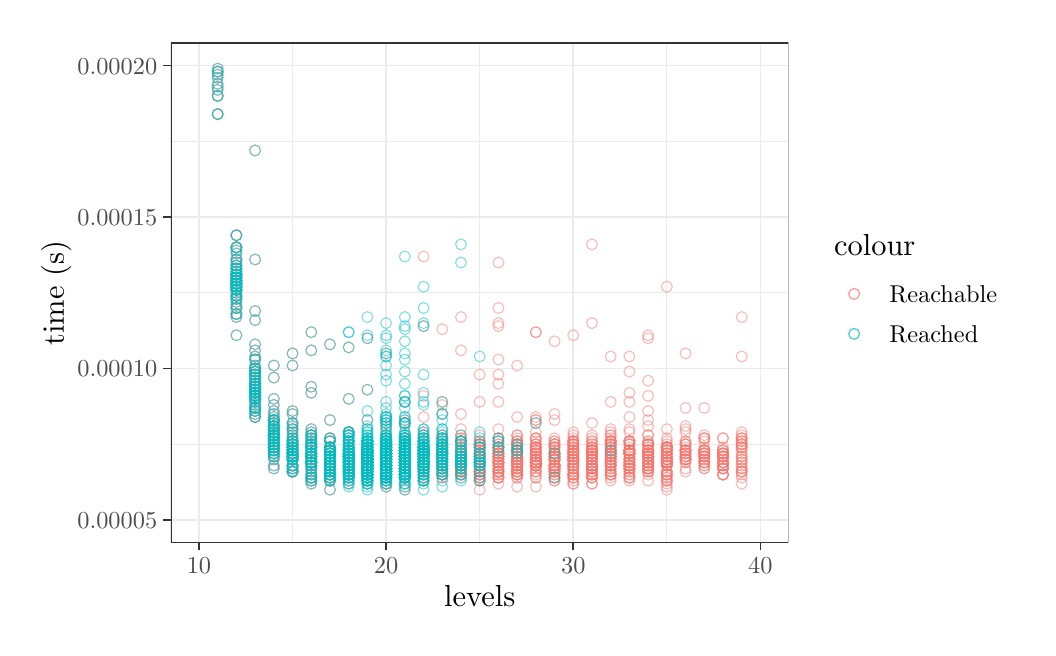
\begin{tikzpicture}[x=1pt,y=1pt]
\definecolor{fillColor}{RGB}{255,255,255}
\path[use as bounding box,fill=fillColor,fill opacity=0.00] (0,0) rectangle (361.35,216.81);
\begin{scope}
\path[clip] (  0.00,  0.00) rectangle (361.35,216.81);
\definecolor{drawColor}{RGB}{255,255,255}
\definecolor{fillColor}{RGB}{255,255,255}

\path[draw=drawColor,line width= 0.6pt,line join=round,line cap=round,fill=fillColor] (  0.00,  0.00) rectangle (361.35,216.81);
\end{scope}
\begin{scope}
\path[clip] ( 51.75, 30.69) rectangle (274.92,211.31);
\definecolor{fillColor}{RGB}{255,255,255}

\path[fill=fillColor] ( 51.75, 30.69) rectangle (274.92,211.31);
\definecolor{drawColor}{gray}{0.92}

\path[draw=drawColor,line width= 0.3pt,line join=round] ( 51.75, 66.26) --
	(274.92, 66.26);

\path[draw=drawColor,line width= 0.3pt,line join=round] ( 51.75,121.00) --
	(274.92,121.00);

\path[draw=drawColor,line width= 0.3pt,line join=round] ( 51.75,175.73) --
	(274.92,175.73);

\path[draw=drawColor,line width= 0.3pt,line join=round] ( 95.71, 30.69) --
	( 95.71,211.31);

\path[draw=drawColor,line width= 0.3pt,line join=round] (163.33, 30.69) --
	(163.33,211.31);

\path[draw=drawColor,line width= 0.3pt,line join=round] (230.96, 30.69) --
	(230.96,211.31);

\path[draw=drawColor,line width= 0.6pt,line join=round] ( 51.75, 38.90) --
	(274.92, 38.90);

\path[draw=drawColor,line width= 0.6pt,line join=round] ( 51.75, 93.63) --
	(274.92, 93.63);

\path[draw=drawColor,line width= 0.6pt,line join=round] ( 51.75,148.37) --
	(274.92,148.37);

\path[draw=drawColor,line width= 0.6pt,line join=round] ( 51.75,203.10) --
	(274.92,203.10);

\path[draw=drawColor,line width= 0.6pt,line join=round] ( 61.90, 30.69) --
	( 61.90,211.31);

\path[draw=drawColor,line width= 0.6pt,line join=round] (129.52, 30.69) --
	(129.52,211.31);

\path[draw=drawColor,line width= 0.6pt,line join=round] (197.15, 30.69) --
	(197.15,211.31);

\path[draw=drawColor,line width= 0.6pt,line join=round] (264.77, 30.69) --
	(264.77,211.31);
\definecolor{drawColor}{RGB}{248,118,109}

\path[draw=drawColor,draw opacity=0.50,line width= 0.4pt,line join=round,line cap=round] ( 68.66,196.53) circle (  1.96);

\path[draw=drawColor,draw opacity=0.50,line width= 0.4pt,line join=round,line cap=round] ( 68.66,200.91) circle (  1.96);

\path[draw=drawColor,draw opacity=0.50,line width= 0.4pt,line join=round,line cap=round] ( 68.66,192.15) circle (  1.96);

\path[draw=drawColor,draw opacity=0.50,line width= 0.4pt,line join=round,line cap=round] ( 68.66,185.58) circle (  1.96);

\path[draw=drawColor,draw opacity=0.50,line width= 0.4pt,line join=round,line cap=round] ( 68.66,202.01) circle (  1.96);

\path[draw=drawColor,draw opacity=0.50,line width= 0.4pt,line join=round,line cap=round] ( 68.66,200.91) circle (  1.96);

\path[draw=drawColor,draw opacity=0.50,line width= 0.4pt,line join=round,line cap=round] ( 68.66,185.58) circle (  1.96);

\path[draw=drawColor,draw opacity=0.50,line width= 0.4pt,line join=round,line cap=round] ( 68.66,192.15) circle (  1.96);

\path[draw=drawColor,draw opacity=0.50,line width= 0.4pt,line join=round,line cap=round] ( 68.66,198.72) circle (  1.96);

\path[draw=drawColor,draw opacity=0.50,line width= 0.4pt,line join=round,line cap=round] ( 75.42,123.19) circle (  1.96);

\path[draw=drawColor,draw opacity=0.50,line width= 0.4pt,line join=round,line cap=round] ( 75.42,136.32) circle (  1.96);

\path[draw=drawColor,draw opacity=0.50,line width= 0.4pt,line join=round,line cap=round] ( 75.42,122.09) circle (  1.96);

\path[draw=drawColor,draw opacity=0.50,line width= 0.4pt,line join=round,line cap=round] ( 75.42,118.81) circle (  1.96);

\path[draw=drawColor,draw opacity=0.50,line width= 0.4pt,line join=round,line cap=round] ( 75.42,126.47) circle (  1.96);

\path[draw=drawColor,draw opacity=0.50,line width= 0.4pt,line join=round,line cap=round] ( 75.42,113.34) circle (  1.96);

\path[draw=drawColor,draw opacity=0.50,line width= 0.4pt,line join=round,line cap=round] ( 75.42,126.47) circle (  1.96);

\path[draw=drawColor,draw opacity=0.50,line width= 0.4pt,line join=round,line cap=round] ( 75.42,112.24) circle (  1.96);

\path[draw=drawColor,draw opacity=0.50,line width= 0.4pt,line join=round,line cap=round] ( 75.42,122.09) circle (  1.96);

\path[draw=drawColor,draw opacity=0.50,line width= 0.4pt,line join=round,line cap=round] ( 75.42,141.80) circle (  1.96);

\path[draw=drawColor,draw opacity=0.50,line width= 0.4pt,line join=round,line cap=round] ( 75.42,119.90) circle (  1.96);

\path[draw=drawColor,draw opacity=0.50,line width= 0.4pt,line join=round,line cap=round] ( 75.42,127.57) circle (  1.96);

\path[draw=drawColor,draw opacity=0.50,line width= 0.4pt,line join=round,line cap=round] ( 75.42,131.94) circle (  1.96);

\path[draw=drawColor,draw opacity=0.50,line width= 0.4pt,line join=round,line cap=round] ( 75.42,127.57) circle (  1.96);

\path[draw=drawColor,draw opacity=0.50,line width= 0.4pt,line join=round,line cap=round] ( 75.42,123.19) circle (  1.96);

\path[draw=drawColor,draw opacity=0.50,line width= 0.4pt,line join=round,line cap=round] ( 75.42,129.76) circle (  1.96);

\path[draw=drawColor,draw opacity=0.50,line width= 0.4pt,line join=round,line cap=round] ( 75.42,129.76) circle (  1.96);

\path[draw=drawColor,draw opacity=0.50,line width= 0.4pt,line join=round,line cap=round] ( 75.42,124.28) circle (  1.96);

\path[draw=drawColor,draw opacity=0.50,line width= 0.4pt,line join=round,line cap=round] ( 75.42,126.47) circle (  1.96);

\path[draw=drawColor,draw opacity=0.50,line width= 0.4pt,line join=round,line cap=round] ( 75.42,119.90) circle (  1.96);

\path[draw=drawColor,draw opacity=0.50,line width= 0.4pt,line join=round,line cap=round] ( 75.42,113.34) circle (  1.96);

\path[draw=drawColor,draw opacity=0.50,line width= 0.4pt,line join=round,line cap=round] ( 75.42,128.66) circle (  1.96);

\path[draw=drawColor,draw opacity=0.50,line width= 0.4pt,line join=round,line cap=round] ( 75.42,125.38) circle (  1.96);

\path[draw=drawColor,draw opacity=0.50,line width= 0.4pt,line join=round,line cap=round] ( 75.42,123.19) circle (  1.96);

\path[draw=drawColor,draw opacity=0.50,line width= 0.4pt,line join=round,line cap=round] ( 75.42,124.28) circle (  1.96);

\path[draw=drawColor,draw opacity=0.50,line width= 0.4pt,line join=round,line cap=round] ( 75.42,123.19) circle (  1.96);

\path[draw=drawColor,draw opacity=0.50,line width= 0.4pt,line join=round,line cap=round] ( 75.42,122.09) circle (  1.96);

\path[draw=drawColor,draw opacity=0.50,line width= 0.4pt,line join=round,line cap=round] ( 75.42,124.28) circle (  1.96);

\path[draw=drawColor,draw opacity=0.50,line width= 0.4pt,line join=round,line cap=round] ( 75.42,126.47) circle (  1.96);

\path[draw=drawColor,draw opacity=0.50,line width= 0.4pt,line join=round,line cap=round] ( 75.42,115.52) circle (  1.96);

\path[draw=drawColor,draw opacity=0.50,line width= 0.4pt,line join=round,line cap=round] ( 75.42,123.19) circle (  1.96);

\path[draw=drawColor,draw opacity=0.50,line width= 0.4pt,line join=round,line cap=round] ( 75.42,127.57) circle (  1.96);

\path[draw=drawColor,draw opacity=0.50,line width= 0.4pt,line join=round,line cap=round] ( 75.42,124.28) circle (  1.96);

\path[draw=drawColor,draw opacity=0.50,line width= 0.4pt,line join=round,line cap=round] ( 82.18, 82.68) circle (  1.96);

\path[draw=drawColor,draw opacity=0.50,line width= 0.4pt,line join=round,line cap=round] ( 82.18, 84.87) circle (  1.96);

\path[draw=drawColor,draw opacity=0.50,line width= 0.4pt,line join=round,line cap=round] ( 82.18, 91.44) circle (  1.96);

\path[draw=drawColor,draw opacity=0.50,line width= 0.4pt,line join=round,line cap=round] ( 82.18, 84.87) circle (  1.96);

\path[draw=drawColor,draw opacity=0.50,line width= 0.4pt,line join=round,line cap=round] ( 82.18, 76.12) circle (  1.96);

\path[draw=drawColor,draw opacity=0.50,line width= 0.4pt,line join=round,line cap=round] ( 82.18,133.04) circle (  1.96);

\path[draw=drawColor,draw opacity=0.50,line width= 0.4pt,line join=round,line cap=round] ( 82.18, 87.06) circle (  1.96);

\path[draw=drawColor,draw opacity=0.50,line width= 0.4pt,line join=round,line cap=round] ( 82.18, 85.97) circle (  1.96);

\path[draw=drawColor,draw opacity=0.50,line width= 0.4pt,line join=round,line cap=round] ( 82.18, 93.63) circle (  1.96);

\path[draw=drawColor,draw opacity=0.50,line width= 0.4pt,line join=round,line cap=round] ( 82.18, 77.21) circle (  1.96);

\path[draw=drawColor,draw opacity=0.50,line width= 0.4pt,line join=round,line cap=round] ( 82.18, 81.59) circle (  1.96);

\path[draw=drawColor,draw opacity=0.50,line width= 0.4pt,line join=round,line cap=round] ( 82.18, 91.44) circle (  1.96);

\path[draw=drawColor,draw opacity=0.50,line width= 0.4pt,line join=round,line cap=round] ( 82.18, 88.16) circle (  1.96);

\path[draw=drawColor,draw opacity=0.50,line width= 0.4pt,line join=round,line cap=round] ( 82.18, 91.44) circle (  1.96);

\path[draw=drawColor,draw opacity=0.50,line width= 0.4pt,line join=round,line cap=round] ( 82.18, 84.87) circle (  1.96);

\path[draw=drawColor,draw opacity=0.50,line width= 0.4pt,line join=round,line cap=round] ( 82.18, 89.25) circle (  1.96);

\path[draw=drawColor,draw opacity=0.50,line width= 0.4pt,line join=round,line cap=round] ( 82.18, 85.97) circle (  1.96);

\path[draw=drawColor,draw opacity=0.50,line width= 0.4pt,line join=round,line cap=round] ( 82.18, 85.97) circle (  1.96);

\path[draw=drawColor,draw opacity=0.50,line width= 0.4pt,line join=round,line cap=round] ( 82.18, 76.12) circle (  1.96);

\path[draw=drawColor,draw opacity=0.50,line width= 0.4pt,line join=round,line cap=round] ( 82.18, 96.91) circle (  1.96);

\path[draw=drawColor,draw opacity=0.50,line width= 0.4pt,line join=round,line cap=round] ( 82.18, 83.78) circle (  1.96);

\path[draw=drawColor,draw opacity=0.50,line width= 0.4pt,line join=round,line cap=round] ( 82.18, 84.87) circle (  1.96);

\path[draw=drawColor,draw opacity=0.50,line width= 0.4pt,line join=round,line cap=round] ( 82.18, 89.25) circle (  1.96);

\path[draw=drawColor,draw opacity=0.50,line width= 0.4pt,line join=round,line cap=round] ( 82.18, 79.40) circle (  1.96);

\path[draw=drawColor,draw opacity=0.50,line width= 0.4pt,line join=round,line cap=round] ( 82.18, 88.16) circle (  1.96);

\path[draw=drawColor,draw opacity=0.50,line width= 0.4pt,line join=round,line cap=round] ( 82.18, 83.78) circle (  1.96);

\path[draw=drawColor,draw opacity=0.50,line width= 0.4pt,line join=round,line cap=round] ( 82.18, 84.87) circle (  1.96);

\path[draw=drawColor,draw opacity=0.50,line width= 0.4pt,line join=round,line cap=round] ( 82.18,102.39) circle (  1.96);

\path[draw=drawColor,draw opacity=0.50,line width= 0.4pt,line join=round,line cap=round] ( 82.18, 83.78) circle (  1.96);

\path[draw=drawColor,draw opacity=0.50,line width= 0.4pt,line join=round,line cap=round] ( 82.18, 83.78) circle (  1.96);

\path[draw=drawColor,draw opacity=0.50,line width= 0.4pt,line join=round,line cap=round] ( 82.18, 79.40) circle (  1.96);

\path[draw=drawColor,draw opacity=0.50,line width= 0.4pt,line join=round,line cap=round] ( 82.18, 82.68) circle (  1.96);

\path[draw=drawColor,draw opacity=0.50,line width= 0.4pt,line join=round,line cap=round] ( 82.18, 93.63) circle (  1.96);

\path[draw=drawColor,draw opacity=0.50,line width= 0.4pt,line join=round,line cap=round] ( 88.95, 69.55) circle (  1.96);

\path[draw=drawColor,draw opacity=0.50,line width= 0.4pt,line join=round,line cap=round] ( 88.95, 75.02) circle (  1.96);

\path[draw=drawColor,draw opacity=0.50,line width= 0.4pt,line join=round,line cap=round] ( 88.95, 72.83) circle (  1.96);

\path[draw=drawColor,draw opacity=0.50,line width= 0.4pt,line join=round,line cap=round] ( 88.95, 78.30) circle (  1.96);

\path[draw=drawColor,draw opacity=0.50,line width= 0.4pt,line join=round,line cap=round] ( 88.95, 73.93) circle (  1.96);

\path[draw=drawColor,draw opacity=0.50,line width= 0.4pt,line join=round,line cap=round] ( 88.95, 68.45) circle (  1.96);

\path[draw=drawColor,draw opacity=0.50,line width= 0.4pt,line join=round,line cap=round] ( 88.95, 75.02) circle (  1.96);

\path[draw=drawColor,draw opacity=0.50,line width= 0.4pt,line join=round,line cap=round] ( 88.95, 69.55) circle (  1.96);

\path[draw=drawColor,draw opacity=0.50,line width= 0.4pt,line join=round,line cap=round] ( 88.95, 71.74) circle (  1.96);

\path[draw=drawColor,draw opacity=0.50,line width= 0.4pt,line join=round,line cap=round] ( 88.95, 65.17) circle (  1.96);

\path[draw=drawColor,draw opacity=0.50,line width= 0.4pt,line join=round,line cap=round] ( 88.95, 94.73) circle (  1.96);

\path[draw=drawColor,draw opacity=0.50,line width= 0.4pt,line join=round,line cap=round] ( 88.95, 69.55) circle (  1.96);

\path[draw=drawColor,draw opacity=0.50,line width= 0.4pt,line join=round,line cap=round] ( 88.95, 64.07) circle (  1.96);

\path[draw=drawColor,draw opacity=0.50,line width= 0.4pt,line join=round,line cap=round] ( 88.95, 76.12) circle (  1.96);

\path[draw=drawColor,draw opacity=0.50,line width= 0.4pt,line join=round,line cap=round] ( 88.95, 65.17) circle (  1.96);

\path[draw=drawColor,draw opacity=0.50,line width= 0.4pt,line join=round,line cap=round] ( 88.95, 65.17) circle (  1.96);

\path[draw=drawColor,draw opacity=0.50,line width= 0.4pt,line join=round,line cap=round] ( 88.95, 82.68) circle (  1.96);

\path[draw=drawColor,draw opacity=0.50,line width= 0.4pt,line join=round,line cap=round] ( 88.95, 69.55) circle (  1.96);

\path[draw=drawColor,draw opacity=0.50,line width= 0.4pt,line join=round,line cap=round] ( 88.95, 68.45) circle (  1.96);

\path[draw=drawColor,draw opacity=0.50,line width= 0.4pt,line join=round,line cap=round] ( 88.95, 70.64) circle (  1.96);

\path[draw=drawColor,draw opacity=0.50,line width= 0.4pt,line join=round,line cap=round] ( 88.95, 62.98) circle (  1.96);

\path[draw=drawColor,draw opacity=0.50,line width= 0.4pt,line join=round,line cap=round] ( 88.95, 66.26) circle (  1.96);

\path[draw=drawColor,draw opacity=0.50,line width= 0.4pt,line join=round,line cap=round] ( 88.95, 71.74) circle (  1.96);

\path[draw=drawColor,draw opacity=0.50,line width= 0.4pt,line join=round,line cap=round] ( 88.95, 69.55) circle (  1.96);

\path[draw=drawColor,draw opacity=0.50,line width= 0.4pt,line join=round,line cap=round] ( 88.95, 58.60) circle (  1.96);

\path[draw=drawColor,draw opacity=0.50,line width= 0.4pt,line join=round,line cap=round] ( 88.95, 71.74) circle (  1.96);

\path[draw=drawColor,draw opacity=0.50,line width= 0.4pt,line join=round,line cap=round] ( 88.95, 80.49) circle (  1.96);

\path[draw=drawColor,draw opacity=0.50,line width= 0.4pt,line join=round,line cap=round] ( 88.95, 75.02) circle (  1.96);

\path[draw=drawColor,draw opacity=0.50,line width= 0.4pt,line join=round,line cap=round] ( 88.95, 69.55) circle (  1.96);

\path[draw=drawColor,draw opacity=0.50,line width= 0.4pt,line join=round,line cap=round] ( 88.95, 72.83) circle (  1.96);

\path[draw=drawColor,draw opacity=0.50,line width= 0.4pt,line join=round,line cap=round] ( 88.95, 90.35) circle (  1.96);

\path[draw=drawColor,draw opacity=0.50,line width= 0.4pt,line join=round,line cap=round] ( 88.95, 72.83) circle (  1.96);

\path[draw=drawColor,draw opacity=0.50,line width= 0.4pt,line join=round,line cap=round] ( 88.95, 64.07) circle (  1.96);

\path[draw=drawColor,draw opacity=0.50,line width= 0.4pt,line join=round,line cap=round] ( 95.71, 65.17) circle (  1.96);

\path[draw=drawColor,draw opacity=0.50,line width= 0.4pt,line join=round,line cap=round] ( 95.71, 64.07) circle (  1.96);

\path[draw=drawColor,draw opacity=0.50,line width= 0.4pt,line join=round,line cap=round] ( 95.71, 71.74) circle (  1.96);

\path[draw=drawColor,draw opacity=0.50,line width= 0.4pt,line join=round,line cap=round] ( 95.71, 94.73) circle (  1.96);

\path[draw=drawColor,draw opacity=0.50,line width= 0.4pt,line join=round,line cap=round] ( 95.71, 62.98) circle (  1.96);

\path[draw=drawColor,draw opacity=0.50,line width= 0.4pt,line join=round,line cap=round] ( 95.71, 66.26) circle (  1.96);

\path[draw=drawColor,draw opacity=0.50,line width= 0.4pt,line join=round,line cap=round] ( 95.71, 64.07) circle (  1.96);

\path[draw=drawColor,draw opacity=0.50,line width= 0.4pt,line join=round,line cap=round] ( 95.71, 78.30) circle (  1.96);

\path[draw=drawColor,draw opacity=0.50,line width= 0.4pt,line join=round,line cap=round] ( 95.71, 62.98) circle (  1.96);

\path[draw=drawColor,draw opacity=0.50,line width= 0.4pt,line join=round,line cap=round] ( 95.71, 62.98) circle (  1.96);

\path[draw=drawColor,draw opacity=0.50,line width= 0.4pt,line join=round,line cap=round] ( 95.71, 64.07) circle (  1.96);

\path[draw=drawColor,draw opacity=0.50,line width= 0.4pt,line join=round,line cap=round] ( 95.71, 64.07) circle (  1.96);

\path[draw=drawColor,draw opacity=0.50,line width= 0.4pt,line join=round,line cap=round] ( 95.71, 62.98) circle (  1.96);

\path[draw=drawColor,draw opacity=0.50,line width= 0.4pt,line join=round,line cap=round] ( 95.71, 68.45) circle (  1.96);

\path[draw=drawColor,draw opacity=0.50,line width= 0.4pt,line join=round,line cap=round] ( 95.71, 65.17) circle (  1.96);

\path[draw=drawColor,draw opacity=0.50,line width= 0.4pt,line join=round,line cap=round] ( 95.71, 56.41) circle (  1.96);

\path[draw=drawColor,draw opacity=0.50,line width= 0.4pt,line join=round,line cap=round] ( 95.71, 99.10) circle (  1.96);

\path[draw=drawColor,draw opacity=0.50,line width= 0.4pt,line join=round,line cap=round] ( 95.71, 66.26) circle (  1.96);

\path[draw=drawColor,draw opacity=0.50,line width= 0.4pt,line join=round,line cap=round] ( 95.71, 72.83) circle (  1.96);

\path[draw=drawColor,draw opacity=0.50,line width= 0.4pt,line join=round,line cap=round] ( 95.71, 66.26) circle (  1.96);

\path[draw=drawColor,draw opacity=0.50,line width= 0.4pt,line join=round,line cap=round] ( 95.71, 64.07) circle (  1.96);

\path[draw=drawColor,draw opacity=0.50,line width= 0.4pt,line join=round,line cap=round] ( 95.71, 56.41) circle (  1.96);

\path[draw=drawColor,draw opacity=0.50,line width= 0.4pt,line join=round,line cap=round] ( 95.71, 67.36) circle (  1.96);

\path[draw=drawColor,draw opacity=0.50,line width= 0.4pt,line join=round,line cap=round] ( 95.71, 61.88) circle (  1.96);

\path[draw=drawColor,draw opacity=0.50,line width= 0.4pt,line join=round,line cap=round] ( 95.71, 60.79) circle (  1.96);

\path[draw=drawColor,draw opacity=0.50,line width= 0.4pt,line join=round,line cap=round] ( 95.71, 64.07) circle (  1.96);

\path[draw=drawColor,draw opacity=0.50,line width= 0.4pt,line join=round,line cap=round] ( 95.71, 61.88) circle (  1.96);

\path[draw=drawColor,draw opacity=0.50,line width= 0.4pt,line join=round,line cap=round] ( 95.71, 62.98) circle (  1.96);

\path[draw=drawColor,draw opacity=0.50,line width= 0.4pt,line join=round,line cap=round] ( 95.71, 60.79) circle (  1.96);

\path[draw=drawColor,draw opacity=0.50,line width= 0.4pt,line join=round,line cap=round] ( 95.71, 62.98) circle (  1.96);

\path[draw=drawColor,draw opacity=0.50,line width= 0.4pt,line join=round,line cap=round] ( 95.71, 73.93) circle (  1.96);

\path[draw=drawColor,draw opacity=0.50,line width= 0.4pt,line join=round,line cap=round] ( 95.71, 71.74) circle (  1.96);

\path[draw=drawColor,draw opacity=0.50,line width= 0.4pt,line join=round,line cap=round] ( 95.71, 60.79) circle (  1.96);

\path[draw=drawColor,draw opacity=0.50,line width= 0.4pt,line join=round,line cap=round] (102.47, 54.22) circle (  1.96);

\path[draw=drawColor,draw opacity=0.50,line width= 0.4pt,line join=round,line cap=round] (102.47, 65.17) circle (  1.96);

\path[draw=drawColor,draw opacity=0.50,line width= 0.4pt,line join=round,line cap=round] (102.47, 62.98) circle (  1.96);

\path[draw=drawColor,draw opacity=0.50,line width= 0.4pt,line join=round,line cap=round] (102.47,100.20) circle (  1.96);

\path[draw=drawColor,draw opacity=0.50,line width= 0.4pt,line join=round,line cap=round] (102.47, 65.17) circle (  1.96);

\path[draw=drawColor,draw opacity=0.50,line width= 0.4pt,line join=round,line cap=round] (102.47, 55.32) circle (  1.96);

\path[draw=drawColor,draw opacity=0.50,line width= 0.4pt,line join=round,line cap=round] (102.47, 59.70) circle (  1.96);

\path[draw=drawColor,draw opacity=0.50,line width= 0.4pt,line join=round,line cap=round] (102.47, 61.88) circle (  1.96);

\path[draw=drawColor,draw opacity=0.50,line width= 0.4pt,line join=round,line cap=round] (102.47, 69.55) circle (  1.96);

\path[draw=drawColor,draw opacity=0.50,line width= 0.4pt,line join=round,line cap=round] (102.47, 87.06) circle (  1.96);

\path[draw=drawColor,draw opacity=0.50,line width= 0.4pt,line join=round,line cap=round] (102.47, 64.07) circle (  1.96);

\path[draw=drawColor,draw opacity=0.50,line width= 0.4pt,line join=round,line cap=round] (102.47, 61.88) circle (  1.96);

\path[draw=drawColor,draw opacity=0.50,line width= 0.4pt,line join=round,line cap=round] (102.47, 68.45) circle (  1.96);

\path[draw=drawColor,draw opacity=0.50,line width= 0.4pt,line join=round,line cap=round] (102.47, 62.98) circle (  1.96);

\path[draw=drawColor,draw opacity=0.50,line width= 0.4pt,line join=round,line cap=round] (102.47, 61.88) circle (  1.96);

\path[draw=drawColor,draw opacity=0.50,line width= 0.4pt,line join=round,line cap=round] (102.47, 65.17) circle (  1.96);

\path[draw=drawColor,draw opacity=0.50,line width= 0.4pt,line join=round,line cap=round] (102.47, 59.70) circle (  1.96);

\path[draw=drawColor,draw opacity=0.50,line width= 0.4pt,line join=round,line cap=round] (102.47, 69.55) circle (  1.96);

\path[draw=drawColor,draw opacity=0.50,line width= 0.4pt,line join=round,line cap=round] (102.47, 57.51) circle (  1.96);

\path[draw=drawColor,draw opacity=0.50,line width= 0.4pt,line join=round,line cap=round] (102.47, 66.26) circle (  1.96);

\path[draw=drawColor,draw opacity=0.50,line width= 0.4pt,line join=round,line cap=round] (102.47, 68.45) circle (  1.96);

\path[draw=drawColor,draw opacity=0.50,line width= 0.4pt,line join=round,line cap=round] (102.47, 67.36) circle (  1.96);

\path[draw=drawColor,draw opacity=0.50,line width= 0.4pt,line join=round,line cap=round] (102.47, 59.70) circle (  1.96);

\path[draw=drawColor,draw opacity=0.50,line width= 0.4pt,line join=round,line cap=round] (102.47, 57.51) circle (  1.96);

\path[draw=drawColor,draw opacity=0.50,line width= 0.4pt,line join=round,line cap=round] (102.47, 59.70) circle (  1.96);

\path[draw=drawColor,draw opacity=0.50,line width= 0.4pt,line join=round,line cap=round] (102.47, 70.64) circle (  1.96);

\path[draw=drawColor,draw opacity=0.50,line width= 0.4pt,line join=round,line cap=round] (102.47, 66.26) circle (  1.96);

\path[draw=drawColor,draw opacity=0.50,line width= 0.4pt,line join=round,line cap=round] (102.47, 65.17) circle (  1.96);

\path[draw=drawColor,draw opacity=0.50,line width= 0.4pt,line join=round,line cap=round] (102.47, 60.79) circle (  1.96);

\path[draw=drawColor,draw opacity=0.50,line width= 0.4pt,line join=round,line cap=round] (102.47, 61.88) circle (  1.96);

\path[draw=drawColor,draw opacity=0.50,line width= 0.4pt,line join=round,line cap=round] (102.47, 66.26) circle (  1.96);

\path[draw=drawColor,draw opacity=0.50,line width= 0.4pt,line join=round,line cap=round] (102.47, 69.55) circle (  1.96);

\path[draw=drawColor,draw opacity=0.50,line width= 0.4pt,line join=round,line cap=round] (102.47, 59.70) circle (  1.96);

\path[draw=drawColor,draw opacity=0.50,line width= 0.4pt,line join=round,line cap=round] (109.23, 60.79) circle (  1.96);

\path[draw=drawColor,draw opacity=0.50,line width= 0.4pt,line join=round,line cap=round] (109.23, 65.17) circle (  1.96);

\path[draw=drawColor,draw opacity=0.50,line width= 0.4pt,line join=round,line cap=round] (109.23, 64.07) circle (  1.96);

\path[draw=drawColor,draw opacity=0.50,line width= 0.4pt,line join=round,line cap=round] (109.23, 65.17) circle (  1.96);

\path[draw=drawColor,draw opacity=0.50,line width= 0.4pt,line join=round,line cap=round] (109.23, 64.07) circle (  1.96);

\path[draw=drawColor,draw opacity=0.50,line width= 0.4pt,line join=round,line cap=round] (109.23, 55.32) circle (  1.96);

\path[draw=drawColor,draw opacity=0.50,line width= 0.4pt,line join=round,line cap=round] (109.23, 67.36) circle (  1.96);

\path[draw=drawColor,draw opacity=0.50,line width= 0.4pt,line join=round,line cap=round] (109.23, 61.88) circle (  1.96);

\path[draw=drawColor,draw opacity=0.50,line width= 0.4pt,line join=round,line cap=round] (109.23, 61.88) circle (  1.96);

\path[draw=drawColor,draw opacity=0.50,line width= 0.4pt,line join=round,line cap=round] (109.23, 62.98) circle (  1.96);

\path[draw=drawColor,draw opacity=0.50,line width= 0.4pt,line join=round,line cap=round] (109.23, 65.17) circle (  1.96);

\path[draw=drawColor,draw opacity=0.50,line width= 0.4pt,line join=round,line cap=round] (109.23, 53.13) circle (  1.96);

\path[draw=drawColor,draw opacity=0.50,line width= 0.4pt,line join=round,line cap=round] (109.23, 68.45) circle (  1.96);

\path[draw=drawColor,draw opacity=0.50,line width= 0.4pt,line join=round,line cap=round] (109.23, 59.70) circle (  1.96);

\path[draw=drawColor,draw opacity=0.50,line width= 0.4pt,line join=round,line cap=round] (109.23, 61.88) circle (  1.96);

\path[draw=drawColor,draw opacity=0.50,line width= 0.4pt,line join=round,line cap=round] (109.23, 62.98) circle (  1.96);

\path[draw=drawColor,draw opacity=0.50,line width= 0.4pt,line join=round,line cap=round] (109.23, 65.17) circle (  1.96);

\path[draw=drawColor,draw opacity=0.50,line width= 0.4pt,line join=round,line cap=round] (109.23, 55.32) circle (  1.96);

\path[draw=drawColor,draw opacity=0.50,line width= 0.4pt,line join=round,line cap=round] (109.23, 53.13) circle (  1.96);

\path[draw=drawColor,draw opacity=0.50,line width= 0.4pt,line join=round,line cap=round] (109.23, 75.02) circle (  1.96);

\path[draw=drawColor,draw opacity=0.50,line width= 0.4pt,line join=round,line cap=round] (109.23, 67.36) circle (  1.96);

\path[draw=drawColor,draw opacity=0.50,line width= 0.4pt,line join=round,line cap=round] (109.23, 57.51) circle (  1.96);

\path[draw=drawColor,draw opacity=0.50,line width= 0.4pt,line join=round,line cap=round] (109.23, 58.60) circle (  1.96);

\path[draw=drawColor,draw opacity=0.50,line width= 0.4pt,line join=round,line cap=round] (109.23,102.39) circle (  1.96);

\path[draw=drawColor,draw opacity=0.50,line width= 0.4pt,line join=round,line cap=round] (109.23, 68.45) circle (  1.96);

\path[draw=drawColor,draw opacity=0.50,line width= 0.4pt,line join=round,line cap=round] (109.23, 56.41) circle (  1.96);

\path[draw=drawColor,draw opacity=0.50,line width= 0.4pt,line join=round,line cap=round] (109.23, 59.70) circle (  1.96);

\path[draw=drawColor,draw opacity=0.50,line width= 0.4pt,line join=round,line cap=round] (109.23, 64.07) circle (  1.96);

\path[draw=drawColor,draw opacity=0.50,line width= 0.4pt,line join=round,line cap=round] (109.23, 61.88) circle (  1.96);

\path[draw=drawColor,draw opacity=0.50,line width= 0.4pt,line join=round,line cap=round] (109.23, 59.70) circle (  1.96);

\path[draw=drawColor,draw opacity=0.50,line width= 0.4pt,line join=round,line cap=round] (109.23, 62.98) circle (  1.96);

\path[draw=drawColor,draw opacity=0.50,line width= 0.4pt,line join=round,line cap=round] (109.23, 61.88) circle (  1.96);

\path[draw=drawColor,draw opacity=0.50,line width= 0.4pt,line join=round,line cap=round] (109.23, 64.07) circle (  1.96);

\path[draw=drawColor,draw opacity=0.50,line width= 0.4pt,line join=round,line cap=round] (116.00, 69.55) circle (  1.96);

\path[draw=drawColor,draw opacity=0.50,line width= 0.4pt,line join=round,line cap=round] (116.00, 70.64) circle (  1.96);

\path[draw=drawColor,draw opacity=0.50,line width= 0.4pt,line join=round,line cap=round] (116.00, 60.79) circle (  1.96);

\path[draw=drawColor,draw opacity=0.50,line width= 0.4pt,line join=round,line cap=round] (116.00, 52.03) circle (  1.96);

\path[draw=drawColor,draw opacity=0.50,line width= 0.4pt,line join=round,line cap=round] (116.00, 61.88) circle (  1.96);

\path[draw=drawColor,draw opacity=0.50,line width= 0.4pt,line join=round,line cap=round] (116.00, 55.32) circle (  1.96);

\path[draw=drawColor,draw opacity=0.50,line width= 0.4pt,line join=round,line cap=round] (116.00, 70.64) circle (  1.96);

\path[draw=drawColor,draw opacity=0.50,line width= 0.4pt,line join=round,line cap=round] (116.00, 58.60) circle (  1.96);

\path[draw=drawColor,draw opacity=0.50,line width= 0.4pt,line join=round,line cap=round] (116.00, 67.36) circle (  1.96);

\path[draw=drawColor,draw opacity=0.50,line width= 0.4pt,line join=round,line cap=round] (116.00, 66.26) circle (  1.96);

\path[draw=drawColor,draw opacity=0.50,line width= 0.4pt,line join=round,line cap=round] (116.00, 59.70) circle (  1.96);

\path[draw=drawColor,draw opacity=0.50,line width= 0.4pt,line join=round,line cap=round] (116.00, 56.41) circle (  1.96);

\path[draw=drawColor,draw opacity=0.50,line width= 0.4pt,line join=round,line cap=round] (116.00, 59.70) circle (  1.96);

\path[draw=drawColor,draw opacity=0.50,line width= 0.4pt,line join=round,line cap=round] (116.00, 61.88) circle (  1.96);

\path[draw=drawColor,draw opacity=0.50,line width= 0.4pt,line join=round,line cap=round] (116.00,101.29) circle (  1.96);

\path[draw=drawColor,draw opacity=0.50,line width= 0.4pt,line join=round,line cap=round] (116.00, 62.98) circle (  1.96);

\path[draw=drawColor,draw opacity=0.50,line width= 0.4pt,line join=round,line cap=round] (116.00, 64.07) circle (  1.96);

\path[draw=drawColor,draw opacity=0.50,line width= 0.4pt,line join=round,line cap=round] (116.00, 59.70) circle (  1.96);

\path[draw=drawColor,draw opacity=0.50,line width= 0.4pt,line join=round,line cap=round] (116.00, 62.98) circle (  1.96);

\path[draw=drawColor,draw opacity=0.50,line width= 0.4pt,line join=round,line cap=round] (116.00, 61.88) circle (  1.96);

\path[draw=drawColor,draw opacity=0.50,line width= 0.4pt,line join=round,line cap=round] (116.00, 62.98) circle (  1.96);

\path[draw=drawColor,draw opacity=0.50,line width= 0.4pt,line join=round,line cap=round] (116.00, 62.98) circle (  1.96);

\path[draw=drawColor,draw opacity=0.50,line width= 0.4pt,line join=round,line cap=round] (116.00, 61.88) circle (  1.96);

\path[draw=drawColor,draw opacity=0.50,line width= 0.4pt,line join=round,line cap=round] (116.00, 67.36) circle (  1.96);

\path[draw=drawColor,draw opacity=0.50,line width= 0.4pt,line join=round,line cap=round] (116.00, 61.88) circle (  1.96);

\path[draw=drawColor,draw opacity=0.50,line width= 0.4pt,line join=round,line cap=round] (116.00, 62.98) circle (  1.96);

\path[draw=drawColor,draw opacity=0.50,line width= 0.4pt,line join=round,line cap=round] (116.00, 62.98) circle (  1.96);

\path[draw=drawColor,draw opacity=0.50,line width= 0.4pt,line join=round,line cap=round] (116.00, 61.88) circle (  1.96);

\path[draw=drawColor,draw opacity=0.50,line width= 0.4pt,line join=round,line cap=round] (116.00, 64.07) circle (  1.96);

\path[draw=drawColor,draw opacity=0.50,line width= 0.4pt,line join=round,line cap=round] (116.00, 55.32) circle (  1.96);

\path[draw=drawColor,draw opacity=0.50,line width= 0.4pt,line join=round,line cap=round] (116.00, 59.70) circle (  1.96);

\path[draw=drawColor,draw opacity=0.50,line width= 0.4pt,line join=round,line cap=round] (116.00, 70.64) circle (  1.96);

\path[draw=drawColor,draw opacity=0.50,line width= 0.4pt,line join=round,line cap=round] (116.00, 60.79) circle (  1.96);

\path[draw=drawColor,draw opacity=0.50,line width= 0.4pt,line join=round,line cap=round] (122.76, 62.98) circle (  1.96);

\path[draw=drawColor,draw opacity=0.50,line width= 0.4pt,line join=round,line cap=round] (122.76, 66.26) circle (  1.96);

\path[draw=drawColor,draw opacity=0.50,line width= 0.4pt,line join=round,line cap=round] (122.76, 60.79) circle (  1.96);

\path[draw=drawColor,draw opacity=0.50,line width= 0.4pt,line join=round,line cap=round] (122.76, 85.97) circle (  1.96);

\path[draw=drawColor,draw opacity=0.50,line width= 0.4pt,line join=round,line cap=round] (122.76, 62.98) circle (  1.96);

\path[draw=drawColor,draw opacity=0.50,line width= 0.4pt,line join=round,line cap=round] (122.76, 56.41) circle (  1.96);

\path[draw=drawColor,draw opacity=0.50,line width= 0.4pt,line join=round,line cap=round] (122.76, 61.88) circle (  1.96);

\path[draw=drawColor,draw opacity=0.50,line width= 0.4pt,line join=round,line cap=round] (122.76, 56.41) circle (  1.96);

\path[draw=drawColor,draw opacity=0.50,line width= 0.4pt,line join=round,line cap=round] (122.76, 62.98) circle (  1.96);

\path[draw=drawColor,draw opacity=0.50,line width= 0.4pt,line join=round,line cap=round] (122.76, 64.07) circle (  1.96);

\path[draw=drawColor,draw opacity=0.50,line width= 0.4pt,line join=round,line cap=round] (122.76, 64.07) circle (  1.96);

\path[draw=drawColor,draw opacity=0.50,line width= 0.4pt,line join=round,line cap=round] (122.76, 64.07) circle (  1.96);

\path[draw=drawColor,draw opacity=0.50,line width= 0.4pt,line join=round,line cap=round] (122.76, 58.60) circle (  1.96);

\path[draw=drawColor,draw opacity=0.50,line width= 0.4pt,line join=round,line cap=round] (122.76, 58.60) circle (  1.96);

\path[draw=drawColor,draw opacity=0.50,line width= 0.4pt,line join=round,line cap=round] (122.76, 59.70) circle (  1.96);

\path[draw=drawColor,draw opacity=0.50,line width= 0.4pt,line join=round,line cap=round] (122.76, 60.79) circle (  1.96);

\path[draw=drawColor,draw opacity=0.50,line width= 0.4pt,line join=round,line cap=round] (122.76, 60.79) circle (  1.96);

\path[draw=drawColor,draw opacity=0.50,line width= 0.4pt,line join=round,line cap=round] (122.76, 64.07) circle (  1.96);

\path[draw=drawColor,draw opacity=0.50,line width= 0.4pt,line join=round,line cap=round] (122.76,104.58) circle (  1.96);

\path[draw=drawColor,draw opacity=0.50,line width= 0.4pt,line join=round,line cap=round] (122.76, 75.02) circle (  1.96);

\path[draw=drawColor,draw opacity=0.50,line width= 0.4pt,line join=round,line cap=round] (122.76, 60.79) circle (  1.96);

\path[draw=drawColor,draw opacity=0.50,line width= 0.4pt,line join=round,line cap=round] (122.76, 55.32) circle (  1.96);

\path[draw=drawColor,draw opacity=0.50,line width= 0.4pt,line join=round,line cap=round] (122.76, 64.07) circle (  1.96);

\path[draw=drawColor,draw opacity=0.50,line width= 0.4pt,line join=round,line cap=round] (122.76, 59.70) circle (  1.96);

\path[draw=drawColor,draw opacity=0.50,line width= 0.4pt,line join=round,line cap=round] (122.76, 61.88) circle (  1.96);

\path[draw=drawColor,draw opacity=0.50,line width= 0.4pt,line join=round,line cap=round] (122.76, 57.51) circle (  1.96);

\path[draw=drawColor,draw opacity=0.50,line width= 0.4pt,line join=round,line cap=round] (122.76, 62.98) circle (  1.96);

\path[draw=drawColor,draw opacity=0.50,line width= 0.4pt,line join=round,line cap=round] (122.76, 55.32) circle (  1.96);

\path[draw=drawColor,draw opacity=0.50,line width= 0.4pt,line join=round,line cap=round] (122.76, 62.98) circle (  1.96);

\path[draw=drawColor,draw opacity=0.50,line width= 0.4pt,line join=round,line cap=round] (122.76, 60.79) circle (  1.96);

\path[draw=drawColor,draw opacity=0.50,line width= 0.4pt,line join=round,line cap=round] (122.76, 60.79) circle (  1.96);

\path[draw=drawColor,draw opacity=0.50,line width= 0.4pt,line join=round,line cap=round] (122.76, 65.17) circle (  1.96);

\path[draw=drawColor,draw opacity=0.50,line width= 0.4pt,line join=round,line cap=round] (122.76, 56.41) circle (  1.96);

\path[draw=drawColor,draw opacity=0.50,line width= 0.4pt,line join=round,line cap=round] (129.52, 64.07) circle (  1.96);

\path[draw=drawColor,draw opacity=0.50,line width= 0.4pt,line join=round,line cap=round] (129.52, 60.79) circle (  1.96);

\path[draw=drawColor,draw opacity=0.50,line width= 0.4pt,line join=round,line cap=round] (129.52, 67.36) circle (  1.96);

\path[draw=drawColor,draw opacity=0.50,line width= 0.4pt,line join=round,line cap=round] (129.52, 64.07) circle (  1.96);

\path[draw=drawColor,draw opacity=0.50,line width= 0.4pt,line join=round,line cap=round] (129.52, 76.12) circle (  1.96);

\path[draw=drawColor,draw opacity=0.50,line width= 0.4pt,line join=round,line cap=round] (129.52, 57.51) circle (  1.96);

\path[draw=drawColor,draw opacity=0.50,line width= 0.4pt,line join=round,line cap=round] (129.52, 58.60) circle (  1.96);

\path[draw=drawColor,draw opacity=0.50,line width= 0.4pt,line join=round,line cap=round] (129.52, 73.93) circle (  1.96);

\path[draw=drawColor,draw opacity=0.50,line width= 0.4pt,line join=round,line cap=round] (129.52, 56.41) circle (  1.96);

\path[draw=drawColor,draw opacity=0.50,line width= 0.4pt,line join=round,line cap=round] (129.52, 55.32) circle (  1.96);

\path[draw=drawColor,draw opacity=0.50,line width= 0.4pt,line join=round,line cap=round] (129.52, 64.07) circle (  1.96);

\path[draw=drawColor,draw opacity=0.50,line width= 0.4pt,line join=round,line cap=round] (129.52, 59.70) circle (  1.96);

\path[draw=drawColor,draw opacity=0.50,line width= 0.4pt,line join=round,line cap=round] (129.52, 59.70) circle (  1.96);

\path[draw=drawColor,draw opacity=0.50,line width= 0.4pt,line join=round,line cap=round] (129.52, 55.32) circle (  1.96);

\path[draw=drawColor,draw opacity=0.50,line width= 0.4pt,line join=round,line cap=round] (129.52, 66.26) circle (  1.96);

\path[draw=drawColor,draw opacity=0.50,line width= 0.4pt,line join=round,line cap=round] (129.52, 65.17) circle (  1.96);

\path[draw=drawColor,draw opacity=0.50,line width= 0.4pt,line join=round,line cap=round] (129.52, 67.36) circle (  1.96);

\path[draw=drawColor,draw opacity=0.50,line width= 0.4pt,line join=round,line cap=round] (129.52, 64.07) circle (  1.96);

\path[draw=drawColor,draw opacity=0.50,line width= 0.4pt,line join=round,line cap=round] (129.52, 56.41) circle (  1.96);

\path[draw=drawColor,draw opacity=0.50,line width= 0.4pt,line join=round,line cap=round] (129.52, 71.74) circle (  1.96);

\path[draw=drawColor,draw opacity=0.50,line width= 0.4pt,line join=round,line cap=round] (129.52, 62.98) circle (  1.96);

\path[draw=drawColor,draw opacity=0.50,line width= 0.4pt,line join=round,line cap=round] (129.52, 66.26) circle (  1.96);

\path[draw=drawColor,draw opacity=0.50,line width= 0.4pt,line join=round,line cap=round] (129.52, 56.41) circle (  1.96);

\path[draw=drawColor,draw opacity=0.50,line width= 0.4pt,line join=round,line cap=round] (129.52, 65.17) circle (  1.96);

\path[draw=drawColor,draw opacity=0.50,line width= 0.4pt,line join=round,line cap=round] (129.52, 99.10) circle (  1.96);

\path[draw=drawColor,draw opacity=0.50,line width= 0.4pt,line join=round,line cap=round] (129.52, 64.07) circle (  1.96);

\path[draw=drawColor,draw opacity=0.50,line width= 0.4pt,line join=round,line cap=round] (129.52, 55.32) circle (  1.96);

\path[draw=drawColor,draw opacity=0.50,line width= 0.4pt,line join=round,line cap=round] (129.52, 58.60) circle (  1.96);

\path[draw=drawColor,draw opacity=0.50,line width= 0.4pt,line join=round,line cap=round] (129.52, 62.98) circle (  1.96);

\path[draw=drawColor,draw opacity=0.50,line width= 0.4pt,line join=round,line cap=round] (129.52, 61.88) circle (  1.96);

\path[draw=drawColor,draw opacity=0.50,line width= 0.4pt,line join=round,line cap=round] (129.52, 62.98) circle (  1.96);

\path[draw=drawColor,draw opacity=0.50,line width= 0.4pt,line join=round,line cap=round] (129.52, 59.70) circle (  1.96);

\path[draw=drawColor,draw opacity=0.50,line width= 0.4pt,line join=round,line cap=round] (129.52, 57.51) circle (  1.96);

\path[draw=drawColor,draw opacity=0.50,line width= 0.4pt,line join=round,line cap=round] (136.28, 64.07) circle (  1.96);

\path[draw=drawColor,draw opacity=0.50,line width= 0.4pt,line join=round,line cap=round] (136.28, 65.17) circle (  1.96);

\path[draw=drawColor,draw opacity=0.50,line width= 0.4pt,line join=round,line cap=round] (136.28, 57.51) circle (  1.96);

\path[draw=drawColor,draw opacity=0.50,line width= 0.4pt,line join=round,line cap=round] (136.28, 65.17) circle (  1.96);

\path[draw=drawColor,draw opacity=0.50,line width= 0.4pt,line join=round,line cap=round] (136.28, 57.51) circle (  1.96);

\path[draw=drawColor,draw opacity=0.50,line width= 0.4pt,line join=round,line cap=round] (136.28, 73.93) circle (  1.96);

\path[draw=drawColor,draw opacity=0.50,line width= 0.4pt,line join=round,line cap=round] (136.28, 67.36) circle (  1.96);

\path[draw=drawColor,draw opacity=0.50,line width= 0.4pt,line join=round,line cap=round] (136.28, 57.51) circle (  1.96);

\path[draw=drawColor,draw opacity=0.50,line width= 0.4pt,line join=round,line cap=round] (136.28, 62.98) circle (  1.96);

\path[draw=drawColor,draw opacity=0.50,line width= 0.4pt,line join=round,line cap=round] (136.28, 70.64) circle (  1.96);

\path[draw=drawColor,draw opacity=0.50,line width= 0.4pt,line join=round,line cap=round] (136.28, 67.36) circle (  1.96);

\path[draw=drawColor,draw opacity=0.50,line width= 0.4pt,line join=round,line cap=round] (136.28, 62.98) circle (  1.96);

\path[draw=drawColor,draw opacity=0.50,line width= 0.4pt,line join=round,line cap=round] (136.28, 68.45) circle (  1.96);

\path[draw=drawColor,draw opacity=0.50,line width= 0.4pt,line join=round,line cap=round] (136.28, 65.17) circle (  1.96);

\path[draw=drawColor,draw opacity=0.50,line width= 0.4pt,line join=round,line cap=round] (136.28, 58.60) circle (  1.96);

\path[draw=drawColor,draw opacity=0.50,line width= 0.4pt,line join=round,line cap=round] (136.28, 59.70) circle (  1.96);

\path[draw=drawColor,draw opacity=0.50,line width= 0.4pt,line join=round,line cap=round] (136.28, 60.79) circle (  1.96);

\path[draw=drawColor,draw opacity=0.50,line width= 0.4pt,line join=round,line cap=round] (136.28, 61.88) circle (  1.96);

\path[draw=drawColor,draw opacity=0.50,line width= 0.4pt,line join=round,line cap=round] (136.28, 55.32) circle (  1.96);

\path[draw=drawColor,draw opacity=0.50,line width= 0.4pt,line join=round,line cap=round] (136.28, 73.93) circle (  1.96);

\path[draw=drawColor,draw opacity=0.50,line width= 0.4pt,line join=round,line cap=round] (136.28, 59.70) circle (  1.96);

\path[draw=drawColor,draw opacity=0.50,line width= 0.4pt,line join=round,line cap=round] (136.28, 67.36) circle (  1.96);

\path[draw=drawColor,draw opacity=0.50,line width= 0.4pt,line join=round,line cap=round] (136.28, 60.79) circle (  1.96);

\path[draw=drawColor,draw opacity=0.50,line width= 0.4pt,line join=round,line cap=round] (136.28, 64.07) circle (  1.96);

\path[draw=drawColor,draw opacity=0.50,line width= 0.4pt,line join=round,line cap=round] (136.28, 67.36) circle (  1.96);

\path[draw=drawColor,draw opacity=0.50,line width= 0.4pt,line join=round,line cap=round] (136.28, 64.07) circle (  1.96);

\path[draw=drawColor,draw opacity=0.50,line width= 0.4pt,line join=round,line cap=round] (136.28, 61.88) circle (  1.96);

\path[draw=drawColor,draw opacity=0.50,line width= 0.4pt,line join=round,line cap=round] (136.28, 75.02) circle (  1.96);

\path[draw=drawColor,draw opacity=0.50,line width= 0.4pt,line join=round,line cap=round] (136.28, 62.98) circle (  1.96);

\path[draw=drawColor,draw opacity=0.50,line width= 0.4pt,line join=round,line cap=round] (136.28, 62.98) circle (  1.96);

\path[draw=drawColor,draw opacity=0.50,line width= 0.4pt,line join=round,line cap=round] (136.28, 67.36) circle (  1.96);

\path[draw=drawColor,draw opacity=0.50,line width= 0.4pt,line join=round,line cap=round] (136.28, 73.93) circle (  1.96);

\path[draw=drawColor,draw opacity=0.50,line width= 0.4pt,line join=round,line cap=round] (136.28, 66.26) circle (  1.96);

\path[draw=drawColor,draw opacity=0.50,line width= 0.4pt,line join=round,line cap=round] (143.05, 64.07) circle (  1.96);

\path[draw=drawColor,draw opacity=0.50,line width= 0.4pt,line join=round,line cap=round] (143.05, 68.45) circle (  1.96);

\path[draw=drawColor,draw opacity=0.50,line width= 0.4pt,line join=round,line cap=round] (143.05, 65.17) circle (  1.96);

\path[draw=drawColor,draw opacity=0.50,line width= 0.4pt,line join=round,line cap=round] (143.05, 54.22) circle (  1.96);

\path[draw=drawColor,draw opacity=0.50,line width= 0.4pt,line join=round,line cap=round] (143.05, 65.17) circle (  1.96);

\path[draw=drawColor,draw opacity=0.50,line width= 0.4pt,line join=round,line cap=round] (143.05,108.96) circle (  1.96);

\path[draw=drawColor,draw opacity=0.50,line width= 0.4pt,line join=round,line cap=round] (143.05, 65.17) circle (  1.96);

\path[draw=drawColor,draw opacity=0.50,line width= 0.4pt,line join=round,line cap=round] (143.05, 67.36) circle (  1.96);

\path[draw=drawColor,draw opacity=0.50,line width= 0.4pt,line join=round,line cap=round] (143.05, 59.70) circle (  1.96);

\path[draw=drawColor,draw opacity=0.50,line width= 0.4pt,line join=round,line cap=round] (143.05, 62.98) circle (  1.96);

\path[draw=drawColor,draw opacity=0.50,line width= 0.4pt,line join=round,line cap=round] (143.05, 65.17) circle (  1.96);

\path[draw=drawColor,draw opacity=0.50,line width= 0.4pt,line join=round,line cap=round] (143.05, 65.17) circle (  1.96);

\path[draw=drawColor,draw opacity=0.50,line width= 0.4pt,line join=round,line cap=round] (143.05, 67.36) circle (  1.96);

\path[draw=drawColor,draw opacity=0.50,line width= 0.4pt,line join=round,line cap=round] (143.05, 61.88) circle (  1.96);

\path[draw=drawColor,draw opacity=0.50,line width= 0.4pt,line join=round,line cap=round] (143.05, 70.64) circle (  1.96);

\path[draw=drawColor,draw opacity=0.50,line width= 0.4pt,line join=round,line cap=round] (143.05, 55.32) circle (  1.96);

\path[draw=drawColor,draw opacity=0.50,line width= 0.4pt,line join=round,line cap=round] (143.05, 66.26) circle (  1.96);

\path[draw=drawColor,draw opacity=0.50,line width= 0.4pt,line join=round,line cap=round] (143.05, 69.55) circle (  1.96);

\path[draw=drawColor,draw opacity=0.50,line width= 0.4pt,line join=round,line cap=round] (143.05, 62.98) circle (  1.96);

\path[draw=drawColor,draw opacity=0.50,line width= 0.4pt,line join=round,line cap=round] (143.05, 58.60) circle (  1.96);

\path[draw=drawColor,draw opacity=0.50,line width= 0.4pt,line join=round,line cap=round] (143.05,134.13) circle (  1.96);

\path[draw=drawColor,draw opacity=0.50,line width= 0.4pt,line join=round,line cap=round] (143.05, 54.22) circle (  1.96);

\path[draw=drawColor,draw opacity=0.50,line width= 0.4pt,line join=round,line cap=round] (143.05, 59.70) circle (  1.96);

\path[draw=drawColor,draw opacity=0.50,line width= 0.4pt,line join=round,line cap=round] (143.05, 62.98) circle (  1.96);

\path[draw=drawColor,draw opacity=0.50,line width= 0.4pt,line join=round,line cap=round] (143.05, 56.41) circle (  1.96);

\path[draw=drawColor,draw opacity=0.50,line width= 0.4pt,line join=round,line cap=round] (143.05, 57.51) circle (  1.96);

\path[draw=drawColor,draw opacity=0.50,line width= 0.4pt,line join=round,line cap=round] (143.05, 59.70) circle (  1.96);

\path[draw=drawColor,draw opacity=0.50,line width= 0.4pt,line join=round,line cap=round] (143.05, 61.88) circle (  1.96);

\path[draw=drawColor,draw opacity=0.50,line width= 0.4pt,line join=round,line cap=round] (143.05, 55.32) circle (  1.96);

\path[draw=drawColor,draw opacity=0.50,line width= 0.4pt,line join=round,line cap=round] (143.05, 62.98) circle (  1.96);

\path[draw=drawColor,draw opacity=0.50,line width= 0.4pt,line join=round,line cap=round] (143.05, 57.51) circle (  1.96);

\path[draw=drawColor,draw opacity=0.50,line width= 0.4pt,line join=round,line cap=round] (143.05, 57.51) circle (  1.96);

\path[draw=drawColor,draw opacity=0.50,line width= 0.4pt,line join=round,line cap=round] (143.05, 53.13) circle (  1.96);

\path[draw=drawColor,draw opacity=0.50,line width= 0.4pt,line join=round,line cap=round] (149.81, 55.32) circle (  1.96);

\path[draw=drawColor,draw opacity=0.50,line width= 0.4pt,line join=round,line cap=round] (149.81, 58.60) circle (  1.96);

\path[draw=drawColor,draw opacity=0.50,line width= 0.4pt,line join=round,line cap=round] (149.81, 62.98) circle (  1.96);

\path[draw=drawColor,draw opacity=0.50,line width= 0.4pt,line join=round,line cap=round] (149.81, 58.60) circle (  1.96);

\path[draw=drawColor,draw opacity=0.50,line width= 0.4pt,line join=round,line cap=round] (149.81, 66.26) circle (  1.96);

\path[draw=drawColor,draw opacity=0.50,line width= 0.4pt,line join=round,line cap=round] (149.81, 64.07) circle (  1.96);

\path[draw=drawColor,draw opacity=0.50,line width= 0.4pt,line join=round,line cap=round] (149.81, 61.88) circle (  1.96);

\path[draw=drawColor,draw opacity=0.50,line width= 0.4pt,line join=round,line cap=round] (149.81, 59.70) circle (  1.96);

\path[draw=drawColor,draw opacity=0.50,line width= 0.4pt,line join=round,line cap=round] (149.81, 64.07) circle (  1.96);

\path[draw=drawColor,draw opacity=0.50,line width= 0.4pt,line join=round,line cap=round] (149.81, 58.60) circle (  1.96);

\path[draw=drawColor,draw opacity=0.50,line width= 0.4pt,line join=round,line cap=round] (149.81, 59.70) circle (  1.96);

\path[draw=drawColor,draw opacity=0.50,line width= 0.4pt,line join=round,line cap=round] (149.81, 66.26) circle (  1.96);

\path[draw=drawColor,draw opacity=0.50,line width= 0.4pt,line join=round,line cap=round] (149.81, 68.45) circle (  1.96);

\path[draw=drawColor,draw opacity=0.50,line width= 0.4pt,line join=round,line cap=round] (149.81, 68.45) circle (  1.96);

\path[draw=drawColor,draw opacity=0.50,line width= 0.4pt,line join=round,line cap=round] (149.81, 60.79) circle (  1.96);

\path[draw=drawColor,draw opacity=0.50,line width= 0.4pt,line join=round,line cap=round] (149.81, 60.79) circle (  1.96);

\path[draw=drawColor,draw opacity=0.50,line width= 0.4pt,line join=round,line cap=round] (149.81, 81.59) circle (  1.96);

\path[draw=drawColor,draw opacity=0.50,line width= 0.4pt,line join=round,line cap=round] (149.81, 60.79) circle (  1.96);

\path[draw=drawColor,draw opacity=0.50,line width= 0.4pt,line join=round,line cap=round] (149.81, 60.79) circle (  1.96);

\path[draw=drawColor,draw opacity=0.50,line width= 0.4pt,line join=round,line cap=round] (149.81, 67.36) circle (  1.96);

\path[draw=drawColor,draw opacity=0.50,line width= 0.4pt,line join=round,line cap=round] (149.81, 62.98) circle (  1.96);

\path[draw=drawColor,draw opacity=0.50,line width= 0.4pt,line join=round,line cap=round] (149.81, 62.98) circle (  1.96);

\path[draw=drawColor,draw opacity=0.50,line width= 0.4pt,line join=round,line cap=round] (149.81, 61.88) circle (  1.96);

\path[draw=drawColor,draw opacity=0.50,line width= 0.4pt,line join=round,line cap=round] (149.81, 59.70) circle (  1.96);

\path[draw=drawColor,draw opacity=0.50,line width= 0.4pt,line join=round,line cap=round] (149.81, 62.98) circle (  1.96);

\path[draw=drawColor,draw opacity=0.50,line width= 0.4pt,line join=round,line cap=round] (149.81, 69.55) circle (  1.96);

\path[draw=drawColor,draw opacity=0.50,line width= 0.4pt,line join=round,line cap=round] (149.81, 62.98) circle (  1.96);

\path[draw=drawColor,draw opacity=0.50,line width= 0.4pt,line join=round,line cap=round] (149.81, 65.17) circle (  1.96);

\path[draw=drawColor,draw opacity=0.50,line width= 0.4pt,line join=round,line cap=round] (149.81, 55.32) circle (  1.96);

\path[draw=drawColor,draw opacity=0.50,line width= 0.4pt,line join=round,line cap=round] (149.81, 54.22) circle (  1.96);

\path[draw=drawColor,draw opacity=0.50,line width= 0.4pt,line join=round,line cap=round] (149.81, 62.98) circle (  1.96);

\path[draw=drawColor,draw opacity=0.50,line width= 0.4pt,line join=round,line cap=round] (149.81, 60.79) circle (  1.96);

\path[draw=drawColor,draw opacity=0.50,line width= 0.4pt,line join=round,line cap=round] (149.81, 68.45) circle (  1.96);

\path[draw=drawColor,draw opacity=0.50,line width= 0.4pt,line join=round,line cap=round] (156.57, 71.74) circle (  1.96);

\path[draw=drawColor,draw opacity=0.50,line width= 0.4pt,line join=round,line cap=round] (156.57, 56.41) circle (  1.96);

\path[draw=drawColor,draw opacity=0.50,line width= 0.4pt,line join=round,line cap=round] (156.57, 56.41) circle (  1.96);

\path[draw=drawColor,draw opacity=0.50,line width= 0.4pt,line join=round,line cap=round] (156.57, 56.41) circle (  1.96);

\path[draw=drawColor,draw opacity=0.50,line width= 0.4pt,line join=round,line cap=round] (156.57, 57.51) circle (  1.96);

\path[draw=drawColor,draw opacity=0.50,line width= 0.4pt,line join=round,line cap=round] (156.57, 68.45) circle (  1.96);

\path[draw=drawColor,draw opacity=0.50,line width= 0.4pt,line join=round,line cap=round] (156.57, 65.17) circle (  1.96);

\path[draw=drawColor,draw opacity=0.50,line width= 0.4pt,line join=round,line cap=round] (156.57, 61.88) circle (  1.96);

\path[draw=drawColor,draw opacity=0.50,line width= 0.4pt,line join=round,line cap=round] (156.57, 56.41) circle (  1.96);

\path[draw=drawColor,draw opacity=0.50,line width= 0.4pt,line join=round,line cap=round] (156.57, 64.07) circle (  1.96);

\path[draw=drawColor,draw opacity=0.50,line width= 0.4pt,line join=round,line cap=round] (156.57, 66.26) circle (  1.96);

\path[draw=drawColor,draw opacity=0.50,line width= 0.4pt,line join=round,line cap=round] (156.57, 67.36) circle (  1.96);

\path[draw=drawColor,draw opacity=0.50,line width= 0.4pt,line join=round,line cap=round] (156.57, 57.51) circle (  1.96);

\path[draw=drawColor,draw opacity=0.50,line width= 0.4pt,line join=round,line cap=round] (156.57, 60.79) circle (  1.96);

\path[draw=drawColor,draw opacity=0.50,line width= 0.4pt,line join=round,line cap=round] (156.57, 64.07) circle (  1.96);

\path[draw=drawColor,draw opacity=0.50,line width= 0.4pt,line join=round,line cap=round] (156.57, 59.70) circle (  1.96);

\path[draw=drawColor,draw opacity=0.50,line width= 0.4pt,line join=round,line cap=round] (156.57, 64.07) circle (  1.96);

\path[draw=drawColor,draw opacity=0.50,line width= 0.4pt,line join=round,line cap=round] (156.57, 59.70) circle (  1.96);

\path[draw=drawColor,draw opacity=0.50,line width= 0.4pt,line join=round,line cap=round] (156.57, 77.21) circle (  1.96);

\path[draw=drawColor,draw opacity=0.50,line width= 0.4pt,line join=round,line cap=round] (156.57, 69.55) circle (  1.96);

\path[draw=drawColor,draw opacity=0.50,line width= 0.4pt,line join=round,line cap=round] (156.57, 62.98) circle (  1.96);

\path[draw=drawColor,draw opacity=0.50,line width= 0.4pt,line join=round,line cap=round] (156.57, 65.17) circle (  1.96);

\path[draw=drawColor,draw opacity=0.50,line width= 0.4pt,line join=round,line cap=round] (156.57,100.20) circle (  1.96);

\path[draw=drawColor,draw opacity=0.50,line width= 0.4pt,line join=round,line cap=round] (156.57, 67.36) circle (  1.96);

\path[draw=drawColor,draw opacity=0.50,line width= 0.4pt,line join=round,line cap=round] (156.57, 68.45) circle (  1.96);

\path[draw=drawColor,draw opacity=0.50,line width= 0.4pt,line join=round,line cap=round] (156.57, 59.70) circle (  1.96);

\path[draw=drawColor,draw opacity=0.50,line width= 0.4pt,line join=round,line cap=round] (156.57, 57.51) circle (  1.96);

\path[draw=drawColor,draw opacity=0.50,line width= 0.4pt,line join=round,line cap=round] (156.57, 62.98) circle (  1.96);

\path[draw=drawColor,draw opacity=0.50,line width= 0.4pt,line join=round,line cap=round] (156.57, 61.88) circle (  1.96);

\path[draw=drawColor,draw opacity=0.50,line width= 0.4pt,line join=round,line cap=round] (156.57, 58.60) circle (  1.96);

\path[draw=drawColor,draw opacity=0.50,line width= 0.4pt,line join=round,line cap=round] (156.57, 65.17) circle (  1.96);

\path[draw=drawColor,draw opacity=0.50,line width= 0.4pt,line join=round,line cap=round] (156.57,112.24) circle (  1.96);

\path[draw=drawColor,draw opacity=0.50,line width= 0.4pt,line join=round,line cap=round] (156.57, 67.36) circle (  1.96);

\path[draw=drawColor,draw opacity=0.50,line width= 0.4pt,line join=round,line cap=round] (163.33, 56.41) circle (  1.96);

\path[draw=drawColor,draw opacity=0.50,line width= 0.4pt,line join=round,line cap=round] (163.33, 61.88) circle (  1.96);

\path[draw=drawColor,draw opacity=0.50,line width= 0.4pt,line join=round,line cap=round] (163.33, 59.70) circle (  1.96);

\path[draw=drawColor,draw opacity=0.50,line width= 0.4pt,line join=round,line cap=round] (163.33, 60.79) circle (  1.96);

\path[draw=drawColor,draw opacity=0.50,line width= 0.4pt,line join=round,line cap=round] (163.33, 65.17) circle (  1.96);

\path[draw=drawColor,draw opacity=0.50,line width= 0.4pt,line join=round,line cap=round] (163.33, 67.36) circle (  1.96);

\path[draw=drawColor,draw opacity=0.50,line width= 0.4pt,line join=round,line cap=round] (163.33, 62.98) circle (  1.96);

\path[draw=drawColor,draw opacity=0.50,line width= 0.4pt,line join=round,line cap=round] (163.33, 62.98) circle (  1.96);

\path[draw=drawColor,draw opacity=0.50,line width= 0.4pt,line join=round,line cap=round] (163.33, 66.26) circle (  1.96);

\path[draw=drawColor,draw opacity=0.50,line width= 0.4pt,line join=round,line cap=round] (163.33, 66.26) circle (  1.96);

\path[draw=drawColor,draw opacity=0.50,line width= 0.4pt,line join=round,line cap=round] (163.33, 67.36) circle (  1.96);

\path[draw=drawColor,draw opacity=0.50,line width= 0.4pt,line join=round,line cap=round] (163.33, 55.32) circle (  1.96);

\path[draw=drawColor,draw opacity=0.50,line width= 0.4pt,line join=round,line cap=round] (163.33, 59.70) circle (  1.96);

\path[draw=drawColor,draw opacity=0.50,line width= 0.4pt,line join=round,line cap=round] (163.33, 59.70) circle (  1.96);

\path[draw=drawColor,draw opacity=0.50,line width= 0.4pt,line join=round,line cap=round] (163.33, 81.59) circle (  1.96);

\path[draw=drawColor,draw opacity=0.50,line width= 0.4pt,line join=round,line cap=round] (163.33, 65.17) circle (  1.96);

\path[draw=drawColor,draw opacity=0.50,line width= 0.4pt,line join=round,line cap=round] (163.33, 66.26) circle (  1.96);

\path[draw=drawColor,draw opacity=0.50,line width= 0.4pt,line join=round,line cap=round] (163.33, 62.98) circle (  1.96);

\path[draw=drawColor,draw opacity=0.50,line width= 0.4pt,line join=round,line cap=round] (163.33, 49.84) circle (  1.96);

\path[draw=drawColor,draw opacity=0.50,line width= 0.4pt,line join=round,line cap=round] (163.33, 61.88) circle (  1.96);

\path[draw=drawColor,draw opacity=0.50,line width= 0.4pt,line join=round,line cap=round] (163.33, 58.60) circle (  1.96);

\path[draw=drawColor,draw opacity=0.50,line width= 0.4pt,line join=round,line cap=round] (163.33, 58.60) circle (  1.96);

\path[draw=drawColor,draw opacity=0.50,line width= 0.4pt,line join=round,line cap=round] (163.33, 67.36) circle (  1.96);

\path[draw=drawColor,draw opacity=0.50,line width= 0.4pt,line join=round,line cap=round] (163.33, 62.98) circle (  1.96);

\path[draw=drawColor,draw opacity=0.50,line width= 0.4pt,line join=round,line cap=round] (163.33, 59.70) circle (  1.96);

\path[draw=drawColor,draw opacity=0.50,line width= 0.4pt,line join=round,line cap=round] (163.33, 62.98) circle (  1.96);

\path[draw=drawColor,draw opacity=0.50,line width= 0.4pt,line join=round,line cap=round] (163.33, 57.51) circle (  1.96);

\path[draw=drawColor,draw opacity=0.50,line width= 0.4pt,line join=round,line cap=round] (163.33, 57.51) circle (  1.96);

\path[draw=drawColor,draw opacity=0.50,line width= 0.4pt,line join=round,line cap=round] (163.33, 66.26) circle (  1.96);

\path[draw=drawColor,draw opacity=0.50,line width= 0.4pt,line join=round,line cap=round] (163.33, 56.41) circle (  1.96);

\path[draw=drawColor,draw opacity=0.50,line width= 0.4pt,line join=round,line cap=round] (163.33, 59.70) circle (  1.96);

\path[draw=drawColor,draw opacity=0.50,line width= 0.4pt,line join=round,line cap=round] (163.33, 62.98) circle (  1.96);

\path[draw=drawColor,draw opacity=0.50,line width= 0.4pt,line join=round,line cap=round] (163.33, 59.70) circle (  1.96);

\path[draw=drawColor,draw opacity=0.50,line width= 0.4pt,line join=round,line cap=round] (170.10, 81.59) circle (  1.96);

\path[draw=drawColor,draw opacity=0.50,line width= 0.4pt,line join=round,line cap=round] (170.10, 55.32) circle (  1.96);

\path[draw=drawColor,draw opacity=0.50,line width= 0.4pt,line join=round,line cap=round] (170.10,131.94) circle (  1.96);

\path[draw=drawColor,draw opacity=0.50,line width= 0.4pt,line join=round,line cap=round] (170.10, 68.45) circle (  1.96);

\path[draw=drawColor,draw opacity=0.50,line width= 0.4pt,line join=round,line cap=round] (170.10, 56.41) circle (  1.96);

\path[draw=drawColor,draw opacity=0.50,line width= 0.4pt,line join=round,line cap=round] (170.10,110.05) circle (  1.96);

\path[draw=drawColor,draw opacity=0.50,line width= 0.4pt,line join=round,line cap=round] (170.10, 65.17) circle (  1.96);

\path[draw=drawColor,draw opacity=0.50,line width= 0.4pt,line join=round,line cap=round] (170.10,115.52) circle (  1.96);

\path[draw=drawColor,draw opacity=0.50,line width= 0.4pt,line join=round,line cap=round] (170.10, 65.17) circle (  1.96);

\path[draw=drawColor,draw opacity=0.50,line width= 0.4pt,line join=round,line cap=round] (170.10, 58.60) circle (  1.96);

\path[draw=drawColor,draw opacity=0.50,line width= 0.4pt,line join=round,line cap=round] (170.10, 59.70) circle (  1.96);

\path[draw=drawColor,draw opacity=0.50,line width= 0.4pt,line join=round,line cap=round] (170.10, 61.88) circle (  1.96);

\path[draw=drawColor,draw opacity=0.50,line width= 0.4pt,line join=round,line cap=round] (170.10, 68.45) circle (  1.96);

\path[draw=drawColor,draw opacity=0.50,line width= 0.4pt,line join=round,line cap=round] (170.10, 59.70) circle (  1.96);

\path[draw=drawColor,draw opacity=0.50,line width= 0.4pt,line join=round,line cap=round] (170.10, 66.26) circle (  1.96);

\path[draw=drawColor,draw opacity=0.50,line width= 0.4pt,line join=round,line cap=round] (170.10, 60.79) circle (  1.96);

\path[draw=drawColor,draw opacity=0.50,line width= 0.4pt,line join=round,line cap=round] (170.10, 62.98) circle (  1.96);

\path[draw=drawColor,draw opacity=0.50,line width= 0.4pt,line join=round,line cap=round] (170.10, 62.98) circle (  1.96);

\path[draw=drawColor,draw opacity=0.50,line width= 0.4pt,line join=round,line cap=round] (170.10, 52.03) circle (  1.96);

\path[draw=drawColor,draw opacity=0.50,line width= 0.4pt,line join=round,line cap=round] (170.10, 62.98) circle (  1.96);

\path[draw=drawColor,draw opacity=0.50,line width= 0.4pt,line join=round,line cap=round] (170.10, 88.16) circle (  1.96);

\path[draw=drawColor,draw opacity=0.50,line width= 0.4pt,line join=round,line cap=round] (170.10, 59.70) circle (  1.96);

\path[draw=drawColor,draw opacity=0.50,line width= 0.4pt,line join=round,line cap=round] (170.10, 62.98) circle (  1.96);

\path[draw=drawColor,draw opacity=0.50,line width= 0.4pt,line join=round,line cap=round] (170.10, 58.60) circle (  1.96);

\path[draw=drawColor,draw opacity=0.50,line width= 0.4pt,line join=round,line cap=round] (170.10, 59.70) circle (  1.96);

\path[draw=drawColor,draw opacity=0.50,line width= 0.4pt,line join=round,line cap=round] (170.10, 64.07) circle (  1.96);

\path[draw=drawColor,draw opacity=0.50,line width= 0.4pt,line join=round,line cap=round] (170.10, 71.74) circle (  1.96);

\path[draw=drawColor,draw opacity=0.50,line width= 0.4pt,line join=round,line cap=round] (170.10, 61.88) circle (  1.96);

\path[draw=drawColor,draw opacity=0.50,line width= 0.4pt,line join=round,line cap=round] (170.10, 54.22) circle (  1.96);

\path[draw=drawColor,draw opacity=0.50,line width= 0.4pt,line join=round,line cap=round] (170.10, 56.41) circle (  1.96);

\path[draw=drawColor,draw opacity=0.50,line width= 0.4pt,line join=round,line cap=round] (170.10, 65.17) circle (  1.96);

\path[draw=drawColor,draw opacity=0.50,line width= 0.4pt,line join=round,line cap=round] (170.10, 68.45) circle (  1.96);

\path[draw=drawColor,draw opacity=0.50,line width= 0.4pt,line join=round,line cap=round] (170.10, 60.79) circle (  1.96);

\path[draw=drawColor,draw opacity=0.50,line width= 0.4pt,line join=round,line cap=round] (176.86, 60.79) circle (  1.96);

\path[draw=drawColor,draw opacity=0.50,line width= 0.4pt,line join=round,line cap=round] (176.86, 59.70) circle (  1.96);

\path[draw=drawColor,draw opacity=0.50,line width= 0.4pt,line join=round,line cap=round] (176.86, 54.22) circle (  1.96);

\path[draw=drawColor,draw opacity=0.50,line width= 0.4pt,line join=round,line cap=round] (176.86, 59.70) circle (  1.96);

\path[draw=drawColor,draw opacity=0.50,line width= 0.4pt,line join=round,line cap=round] (176.86, 59.70) circle (  1.96);

\path[draw=drawColor,draw opacity=0.50,line width= 0.4pt,line join=round,line cap=round] (176.86, 69.55) circle (  1.96);

\path[draw=drawColor,draw opacity=0.50,line width= 0.4pt,line join=round,line cap=round] (176.86, 62.98) circle (  1.96);

\path[draw=drawColor,draw opacity=0.50,line width= 0.4pt,line join=round,line cap=round] (176.86, 64.07) circle (  1.96);

\path[draw=drawColor,draw opacity=0.50,line width= 0.4pt,line join=round,line cap=round] (176.86, 59.70) circle (  1.96);

\path[draw=drawColor,draw opacity=0.50,line width= 0.4pt,line join=round,line cap=round] (176.86, 64.07) circle (  1.96);

\path[draw=drawColor,draw opacity=0.50,line width= 0.4pt,line join=round,line cap=round] (176.86, 65.17) circle (  1.96);

\path[draw=drawColor,draw opacity=0.50,line width= 0.4pt,line join=round,line cap=round] (176.86, 64.07) circle (  1.96);

\path[draw=drawColor,draw opacity=0.50,line width= 0.4pt,line join=round,line cap=round] (176.86, 60.79) circle (  1.96);

\path[draw=drawColor,draw opacity=0.50,line width= 0.4pt,line join=round,line cap=round] (176.86, 60.79) circle (  1.96);

\path[draw=drawColor,draw opacity=0.50,line width= 0.4pt,line join=round,line cap=round] (176.86, 60.79) circle (  1.96);

\path[draw=drawColor,draw opacity=0.50,line width= 0.4pt,line join=round,line cap=round] (176.86, 94.73) circle (  1.96);

\path[draw=drawColor,draw opacity=0.50,line width= 0.4pt,line join=round,line cap=round] (176.86, 67.36) circle (  1.96);

\path[draw=drawColor,draw opacity=0.50,line width= 0.4pt,line join=round,line cap=round] (176.86, 64.07) circle (  1.96);

\path[draw=drawColor,draw opacity=0.50,line width= 0.4pt,line join=round,line cap=round] (176.86, 66.26) circle (  1.96);

\path[draw=drawColor,draw opacity=0.50,line width= 0.4pt,line join=round,line cap=round] (176.86, 67.36) circle (  1.96);

\path[draw=drawColor,draw opacity=0.50,line width= 0.4pt,line join=round,line cap=round] (176.86, 62.98) circle (  1.96);

\path[draw=drawColor,draw opacity=0.50,line width= 0.4pt,line join=round,line cap=round] (176.86, 57.51) circle (  1.96);

\path[draw=drawColor,draw opacity=0.50,line width= 0.4pt,line join=round,line cap=round] (176.86, 61.88) circle (  1.96);

\path[draw=drawColor,draw opacity=0.50,line width= 0.4pt,line join=round,line cap=round] (176.86, 67.36) circle (  1.96);

\path[draw=drawColor,draw opacity=0.50,line width= 0.4pt,line join=round,line cap=round] (176.86, 59.70) circle (  1.96);

\path[draw=drawColor,draw opacity=0.50,line width= 0.4pt,line join=round,line cap=round] (176.86, 50.94) circle (  1.96);

\path[draw=drawColor,draw opacity=0.50,line width= 0.4pt,line join=round,line cap=round] (176.86, 66.26) circle (  1.96);

\path[draw=drawColor,draw opacity=0.50,line width= 0.4pt,line join=round,line cap=round] (176.86, 60.79) circle (  1.96);

\path[draw=drawColor,draw opacity=0.50,line width= 0.4pt,line join=round,line cap=round] (176.86, 55.32) circle (  1.96);

\path[draw=drawColor,draw opacity=0.50,line width= 0.4pt,line join=round,line cap=round] (176.86, 66.26) circle (  1.96);

\path[draw=drawColor,draw opacity=0.50,line width= 0.4pt,line join=round,line cap=round] (176.86, 58.60) circle (  1.96);

\path[draw=drawColor,draw opacity=0.50,line width= 0.4pt,line join=round,line cap=round] (176.86, 61.88) circle (  1.96);

\path[draw=drawColor,draw opacity=0.50,line width= 0.4pt,line join=round,line cap=round] (176.86, 55.32) circle (  1.96);

\path[draw=drawColor,draw opacity=0.50,line width= 0.4pt,line join=round,line cap=round] (183.62, 59.70) circle (  1.96);

\path[draw=drawColor,draw opacity=0.50,line width= 0.4pt,line join=round,line cap=round] (183.62,106.77) circle (  1.96);

\path[draw=drawColor,draw opacity=0.50,line width= 0.4pt,line join=round,line cap=round] (183.62, 62.98) circle (  1.96);

\path[draw=drawColor,draw opacity=0.50,line width= 0.4pt,line join=round,line cap=round] (183.62, 64.07) circle (  1.96);

\path[draw=drawColor,draw opacity=0.50,line width= 0.4pt,line join=round,line cap=round] (183.62, 66.26) circle (  1.96);

\path[draw=drawColor,draw opacity=0.50,line width= 0.4pt,line join=round,line cap=round] (183.62, 60.79) circle (  1.96);

\path[draw=drawColor,draw opacity=0.50,line width= 0.4pt,line join=round,line cap=round] (183.62, 75.02) circle (  1.96);

\path[draw=drawColor,draw opacity=0.50,line width= 0.4pt,line join=round,line cap=round] (183.62, 60.79) circle (  1.96);

\path[draw=drawColor,draw opacity=0.50,line width= 0.4pt,line join=round,line cap=round] (183.62, 59.70) circle (  1.96);

\path[draw=drawColor,draw opacity=0.50,line width= 0.4pt,line join=round,line cap=round] (183.62, 60.79) circle (  1.96);

\path[draw=drawColor,draw opacity=0.50,line width= 0.4pt,line join=round,line cap=round] (183.62, 65.17) circle (  1.96);

\path[draw=drawColor,draw opacity=0.50,line width= 0.4pt,line join=round,line cap=round] (183.62, 60.79) circle (  1.96);

\path[draw=drawColor,draw opacity=0.50,line width= 0.4pt,line join=round,line cap=round] (183.62, 65.17) circle (  1.96);

\path[draw=drawColor,draw opacity=0.50,line width= 0.4pt,line join=round,line cap=round] (183.62, 68.45) circle (  1.96);

\path[draw=drawColor,draw opacity=0.50,line width= 0.4pt,line join=round,line cap=round] (183.62, 68.45) circle (  1.96);

\path[draw=drawColor,draw opacity=0.50,line width= 0.4pt,line join=round,line cap=round] (183.62, 59.70) circle (  1.96);

\path[draw=drawColor,draw opacity=0.50,line width= 0.4pt,line join=round,line cap=round] (183.62, 59.70) circle (  1.96);

\path[draw=drawColor,draw opacity=0.50,line width= 0.4pt,line join=round,line cap=round] (183.62, 59.70) circle (  1.96);

\path[draw=drawColor,draw opacity=0.50,line width= 0.4pt,line join=round,line cap=round] (183.62, 64.07) circle (  1.96);

\path[draw=drawColor,draw opacity=0.50,line width= 0.4pt,line join=round,line cap=round] (183.62, 65.17) circle (  1.96);

\path[draw=drawColor,draw opacity=0.50,line width= 0.4pt,line join=round,line cap=round] (183.62, 56.41) circle (  1.96);

\path[draw=drawColor,draw opacity=0.50,line width= 0.4pt,line join=round,line cap=round] (183.62, 59.70) circle (  1.96);

\path[draw=drawColor,draw opacity=0.50,line width= 0.4pt,line join=round,line cap=round] (183.62, 75.02) circle (  1.96);

\path[draw=drawColor,draw opacity=0.50,line width= 0.4pt,line join=round,line cap=round] (183.62, 55.32) circle (  1.96);

\path[draw=drawColor,draw opacity=0.50,line width= 0.4pt,line join=round,line cap=round] (183.62, 59.70) circle (  1.96);

\path[draw=drawColor,draw opacity=0.50,line width= 0.4pt,line join=round,line cap=round] (183.62, 58.60) circle (  1.96);

\path[draw=drawColor,draw opacity=0.50,line width= 0.4pt,line join=round,line cap=round] (183.62, 60.79) circle (  1.96);

\path[draw=drawColor,draw opacity=0.50,line width= 0.4pt,line join=round,line cap=round] (183.62, 57.51) circle (  1.96);

\path[draw=drawColor,draw opacity=0.50,line width= 0.4pt,line join=round,line cap=round] (183.62, 60.79) circle (  1.96);

\path[draw=drawColor,draw opacity=0.50,line width= 0.4pt,line join=round,line cap=round] (183.62, 66.26) circle (  1.96);

\path[draw=drawColor,draw opacity=0.50,line width= 0.4pt,line join=round,line cap=round] (183.62, 61.88) circle (  1.96);

\path[draw=drawColor,draw opacity=0.50,line width= 0.4pt,line join=round,line cap=round] (183.62, 59.70) circle (  1.96);

\path[draw=drawColor,draw opacity=0.50,line width= 0.4pt,line join=round,line cap=round] (183.62, 70.64) circle (  1.96);

\path[draw=drawColor,draw opacity=0.50,line width= 0.4pt,line join=round,line cap=round] (190.38, 61.88) circle (  1.96);

\path[draw=drawColor,draw opacity=0.50,line width= 0.4pt,line join=round,line cap=round] (190.38, 64.07) circle (  1.96);

\path[draw=drawColor,draw opacity=0.50,line width= 0.4pt,line join=round,line cap=round] (190.38, 65.17) circle (  1.96);

\path[draw=drawColor,draw opacity=0.50,line width= 0.4pt,line join=round,line cap=round] (190.38, 61.88) circle (  1.96);

\path[draw=drawColor,draw opacity=0.50,line width= 0.4pt,line join=round,line cap=round] (190.38, 68.45) circle (  1.96);

\path[draw=drawColor,draw opacity=0.50,line width= 0.4pt,line join=round,line cap=round] (190.38, 66.26) circle (  1.96);

\path[draw=drawColor,draw opacity=0.50,line width= 0.4pt,line join=round,line cap=round] (190.38, 75.02) circle (  1.96);

\path[draw=drawColor,draw opacity=0.50,line width= 0.4pt,line join=round,line cap=round] (190.38, 67.36) circle (  1.96);

\path[draw=drawColor,draw opacity=0.50,line width= 0.4pt,line join=round,line cap=round] (190.38, 57.51) circle (  1.96);

\path[draw=drawColor,draw opacity=0.50,line width= 0.4pt,line join=round,line cap=round] (190.38, 60.79) circle (  1.96);

\path[draw=drawColor,draw opacity=0.50,line width= 0.4pt,line join=round,line cap=round] (190.38, 62.98) circle (  1.96);

\path[draw=drawColor,draw opacity=0.50,line width= 0.4pt,line join=round,line cap=round] (190.38, 61.88) circle (  1.96);

\path[draw=drawColor,draw opacity=0.50,line width= 0.4pt,line join=round,line cap=round] (190.38, 60.79) circle (  1.96);

\path[draw=drawColor,draw opacity=0.50,line width= 0.4pt,line join=round,line cap=round] (190.38, 66.26) circle (  1.96);

\path[draw=drawColor,draw opacity=0.50,line width= 0.4pt,line join=round,line cap=round] (190.38, 66.26) circle (  1.96);

\path[draw=drawColor,draw opacity=0.50,line width= 0.4pt,line join=round,line cap=round] (190.38, 57.51) circle (  1.96);

\path[draw=drawColor,draw opacity=0.50,line width= 0.4pt,line join=round,line cap=round] (190.38, 65.17) circle (  1.96);

\path[draw=drawColor,draw opacity=0.50,line width= 0.4pt,line join=round,line cap=round] (190.38, 56.41) circle (  1.96);

\path[draw=drawColor,draw opacity=0.50,line width= 0.4pt,line join=round,line cap=round] (190.38, 57.51) circle (  1.96);

\path[draw=drawColor,draw opacity=0.50,line width= 0.4pt,line join=round,line cap=round] (190.38, 67.36) circle (  1.96);

\path[draw=drawColor,draw opacity=0.50,line width= 0.4pt,line join=round,line cap=round] (190.38, 62.98) circle (  1.96);

\path[draw=drawColor,draw opacity=0.50,line width= 0.4pt,line join=round,line cap=round] (190.38, 58.60) circle (  1.96);

\path[draw=drawColor,draw opacity=0.50,line width= 0.4pt,line join=round,line cap=round] (190.38, 54.22) circle (  1.96);

\path[draw=drawColor,draw opacity=0.50,line width= 0.4pt,line join=round,line cap=round] (190.38, 61.88) circle (  1.96);

\path[draw=drawColor,draw opacity=0.50,line width= 0.4pt,line join=round,line cap=round] (190.38, 60.79) circle (  1.96);

\path[draw=drawColor,draw opacity=0.50,line width= 0.4pt,line join=round,line cap=round] (190.38, 55.32) circle (  1.96);

\path[draw=drawColor,draw opacity=0.50,line width= 0.4pt,line join=round,line cap=round] (190.38, 62.98) circle (  1.96);

\path[draw=drawColor,draw opacity=0.50,line width= 0.4pt,line join=round,line cap=round] (190.38, 62.98) circle (  1.96);

\path[draw=drawColor,draw opacity=0.50,line width= 0.4pt,line join=round,line cap=round] (190.38, 60.79) circle (  1.96);

\path[draw=drawColor,draw opacity=0.50,line width= 0.4pt,line join=round,line cap=round] (190.38, 54.22) circle (  1.96);

\path[draw=drawColor,draw opacity=0.50,line width= 0.4pt,line join=round,line cap=round] (190.38, 58.60) circle (  1.96);

\path[draw=drawColor,draw opacity=0.50,line width= 0.4pt,line join=round,line cap=round] (190.38, 58.60) circle (  1.96);

\path[draw=drawColor,draw opacity=0.50,line width= 0.4pt,line join=round,line cap=round] (190.38, 58.60) circle (  1.96);

\path[draw=drawColor,draw opacity=0.50,line width= 0.4pt,line join=round,line cap=round] (197.15, 62.98) circle (  1.96);

\path[draw=drawColor,draw opacity=0.50,line width= 0.4pt,line join=round,line cap=round] (197.15, 54.22) circle (  1.96);

\path[draw=drawColor,draw opacity=0.50,line width= 0.4pt,line join=round,line cap=round] (197.15, 70.64) circle (  1.96);

\path[draw=drawColor,draw opacity=0.50,line width= 0.4pt,line join=round,line cap=round] (197.15, 66.26) circle (  1.96);

\path[draw=drawColor,draw opacity=0.50,line width= 0.4pt,line join=round,line cap=round] (197.15, 61.88) circle (  1.96);

\path[draw=drawColor,draw opacity=0.50,line width= 0.4pt,line join=round,line cap=round] (197.15, 52.03) circle (  1.96);

\path[draw=drawColor,draw opacity=0.50,line width= 0.4pt,line join=round,line cap=round] (197.15, 61.88) circle (  1.96);

\path[draw=drawColor,draw opacity=0.50,line width= 0.4pt,line join=round,line cap=round] (197.15, 64.07) circle (  1.96);

\path[draw=drawColor,draw opacity=0.50,line width= 0.4pt,line join=round,line cap=round] (197.15, 67.36) circle (  1.96);

\path[draw=drawColor,draw opacity=0.50,line width= 0.4pt,line join=round,line cap=round] (197.15, 55.32) circle (  1.96);

\path[draw=drawColor,draw opacity=0.50,line width= 0.4pt,line join=round,line cap=round] (197.15, 67.36) circle (  1.96);

\path[draw=drawColor,draw opacity=0.50,line width= 0.4pt,line join=round,line cap=round] (197.15, 64.07) circle (  1.96);

\path[draw=drawColor,draw opacity=0.50,line width= 0.4pt,line join=round,line cap=round] (197.15, 68.45) circle (  1.96);

\path[draw=drawColor,draw opacity=0.50,line width= 0.4pt,line join=round,line cap=round] (197.15, 66.26) circle (  1.96);

\path[draw=drawColor,draw opacity=0.50,line width= 0.4pt,line join=round,line cap=round] (197.15, 69.55) circle (  1.96);

\path[draw=drawColor,draw opacity=0.50,line width= 0.4pt,line join=round,line cap=round] (197.15, 55.32) circle (  1.96);

\path[draw=drawColor,draw opacity=0.50,line width= 0.4pt,line join=round,line cap=round] (197.15, 62.98) circle (  1.96);

\path[draw=drawColor,draw opacity=0.50,line width= 0.4pt,line join=round,line cap=round] (197.15, 59.70) circle (  1.96);

\path[draw=drawColor,draw opacity=0.50,line width= 0.4pt,line join=round,line cap=round] (197.15, 62.98) circle (  1.96);

\path[draw=drawColor,draw opacity=0.50,line width= 0.4pt,line join=round,line cap=round] (197.15, 59.70) circle (  1.96);

\path[draw=drawColor,draw opacity=0.50,line width= 0.4pt,line join=round,line cap=round] (197.15, 66.26) circle (  1.96);

\path[draw=drawColor,draw opacity=0.50,line width= 0.4pt,line join=round,line cap=round] (197.15, 64.07) circle (  1.96);

\path[draw=drawColor,draw opacity=0.50,line width= 0.4pt,line join=round,line cap=round] (197.15, 66.26) circle (  1.96);

\path[draw=drawColor,draw opacity=0.50,line width= 0.4pt,line join=round,line cap=round] (197.15, 58.60) circle (  1.96);

\path[draw=drawColor,draw opacity=0.50,line width= 0.4pt,line join=round,line cap=round] (197.15, 62.98) circle (  1.96);

\path[draw=drawColor,draw opacity=0.50,line width= 0.4pt,line join=round,line cap=round] (197.15, 66.26) circle (  1.96);

\path[draw=drawColor,draw opacity=0.50,line width= 0.4pt,line join=round,line cap=round] (197.15, 67.36) circle (  1.96);

\path[draw=drawColor,draw opacity=0.50,line width= 0.4pt,line join=round,line cap=round] (197.15, 54.22) circle (  1.96);

\path[draw=drawColor,draw opacity=0.50,line width= 0.4pt,line join=round,line cap=round] (197.15, 60.79) circle (  1.96);

\path[draw=drawColor,draw opacity=0.50,line width= 0.4pt,line join=round,line cap=round] (197.15, 62.98) circle (  1.96);

\path[draw=drawColor,draw opacity=0.50,line width= 0.4pt,line join=round,line cap=round] (197.15, 64.07) circle (  1.96);

\path[draw=drawColor,draw opacity=0.50,line width= 0.4pt,line join=round,line cap=round] (197.15, 60.79) circle (  1.96);

\path[draw=drawColor,draw opacity=0.50,line width= 0.4pt,line join=round,line cap=round] (197.15, 65.17) circle (  1.96);

\path[draw=drawColor,draw opacity=0.50,line width= 0.4pt,line join=round,line cap=round] (203.91, 64.07) circle (  1.96);

\path[draw=drawColor,draw opacity=0.50,line width= 0.4pt,line join=round,line cap=round] (203.91, 68.45) circle (  1.96);

\path[draw=drawColor,draw opacity=0.50,line width= 0.4pt,line join=round,line cap=round] (203.91, 61.88) circle (  1.96);

\path[draw=drawColor,draw opacity=0.50,line width= 0.4pt,line join=round,line cap=round] (203.91, 60.79) circle (  1.96);

\path[draw=drawColor,draw opacity=0.50,line width= 0.4pt,line join=round,line cap=round] (203.91, 52.03) circle (  1.96);

\path[draw=drawColor,draw opacity=0.50,line width= 0.4pt,line join=round,line cap=round] (203.91, 54.22) circle (  1.96);

\path[draw=drawColor,draw opacity=0.50,line width= 0.4pt,line join=round,line cap=round] (203.91, 57.51) circle (  1.96);

\path[draw=drawColor,draw opacity=0.50,line width= 0.4pt,line join=round,line cap=round] (203.91, 69.55) circle (  1.96);

\path[draw=drawColor,draw opacity=0.50,line width= 0.4pt,line join=round,line cap=round] (203.91, 67.36) circle (  1.96);

\path[draw=drawColor,draw opacity=0.50,line width= 0.4pt,line join=round,line cap=round] (203.91, 57.51) circle (  1.96);

\path[draw=drawColor,draw opacity=0.50,line width= 0.4pt,line join=round,line cap=round] (203.91, 56.41) circle (  1.96);

\path[draw=drawColor,draw opacity=0.50,line width= 0.4pt,line join=round,line cap=round] (203.91, 66.26) circle (  1.96);

\path[draw=drawColor,draw opacity=0.50,line width= 0.4pt,line join=round,line cap=round] (203.91, 57.51) circle (  1.96);

\path[draw=drawColor,draw opacity=0.50,line width= 0.4pt,line join=round,line cap=round] (203.91, 58.60) circle (  1.96);

\path[draw=drawColor,draw opacity=0.50,line width= 0.4pt,line join=round,line cap=round] (203.91, 59.70) circle (  1.96);

\path[draw=drawColor,draw opacity=0.50,line width= 0.4pt,line join=round,line cap=round] (203.91, 55.32) circle (  1.96);

\path[draw=drawColor,draw opacity=0.50,line width= 0.4pt,line join=round,line cap=round] (203.91, 66.26) circle (  1.96);

\path[draw=drawColor,draw opacity=0.50,line width= 0.4pt,line join=round,line cap=round] (203.91, 60.79) circle (  1.96);

\path[draw=drawColor,draw opacity=0.50,line width= 0.4pt,line join=round,line cap=round] (203.91, 60.79) circle (  1.96);

\path[draw=drawColor,draw opacity=0.50,line width= 0.4pt,line join=round,line cap=round] (203.91, 65.17) circle (  1.96);

\path[draw=drawColor,draw opacity=0.50,line width= 0.4pt,line join=round,line cap=round] (203.91, 61.88) circle (  1.96);

\path[draw=drawColor,draw opacity=0.50,line width= 0.4pt,line join=round,line cap=round] (203.91, 64.07) circle (  1.96);

\path[draw=drawColor,draw opacity=0.50,line width= 0.4pt,line join=round,line cap=round] (203.91, 65.17) circle (  1.96);

\path[draw=drawColor,draw opacity=0.50,line width= 0.4pt,line join=round,line cap=round] (203.91, 62.98) circle (  1.96);

\path[draw=drawColor,draw opacity=0.50,line width= 0.4pt,line join=round,line cap=round] (203.91, 52.03) circle (  1.96);

\path[draw=drawColor,draw opacity=0.50,line width= 0.4pt,line join=round,line cap=round] (203.91, 64.07) circle (  1.96);

\path[draw=drawColor,draw opacity=0.50,line width= 0.4pt,line join=round,line cap=round] (203.91, 65.17) circle (  1.96);

\path[draw=drawColor,draw opacity=0.50,line width= 0.4pt,line join=round,line cap=round] (203.91, 55.32) circle (  1.96);

\path[draw=drawColor,draw opacity=0.50,line width= 0.4pt,line join=round,line cap=round] (203.91, 64.07) circle (  1.96);

\path[draw=drawColor,draw opacity=0.50,line width= 0.4pt,line join=round,line cap=round] (203.91, 61.88) circle (  1.96);

\path[draw=drawColor,draw opacity=0.50,line width= 0.4pt,line join=round,line cap=round] (203.91, 67.36) circle (  1.96);

\path[draw=drawColor,draw opacity=0.50,line width= 0.4pt,line join=round,line cap=round] (203.91, 64.07) circle (  1.96);

\path[draw=drawColor,draw opacity=0.50,line width= 0.4pt,line join=round,line cap=round] (203.91, 59.70) circle (  1.96);

\path[draw=drawColor,draw opacity=0.50,line width= 0.4pt,line join=round,line cap=round] (210.67, 60.79) circle (  1.96);

\path[draw=drawColor,draw opacity=0.50,line width= 0.4pt,line join=round,line cap=round] (210.67, 64.07) circle (  1.96);

\path[draw=drawColor,draw opacity=0.50,line width= 0.4pt,line join=round,line cap=round] (210.67, 81.59) circle (  1.96);

\path[draw=drawColor,draw opacity=0.50,line width= 0.4pt,line join=round,line cap=round] (210.67, 66.26) circle (  1.96);

\path[draw=drawColor,draw opacity=0.50,line width= 0.4pt,line join=round,line cap=round] (210.67, 56.41) circle (  1.96);

\path[draw=drawColor,draw opacity=0.50,line width= 0.4pt,line join=round,line cap=round] (210.67, 59.70) circle (  1.96);

\path[draw=drawColor,draw opacity=0.50,line width= 0.4pt,line join=round,line cap=round] (210.67, 61.88) circle (  1.96);

\path[draw=drawColor,draw opacity=0.50,line width= 0.4pt,line join=round,line cap=round] (210.67, 62.98) circle (  1.96);

\path[draw=drawColor,draw opacity=0.50,line width= 0.4pt,line join=round,line cap=round] (210.67, 62.98) circle (  1.96);

\path[draw=drawColor,draw opacity=0.50,line width= 0.4pt,line join=round,line cap=round] (210.67, 64.07) circle (  1.96);

\path[draw=drawColor,draw opacity=0.50,line width= 0.4pt,line join=round,line cap=round] (210.67, 67.36) circle (  1.96);

\path[draw=drawColor,draw opacity=0.50,line width= 0.4pt,line join=round,line cap=round] (210.67, 66.26) circle (  1.96);

\path[draw=drawColor,draw opacity=0.50,line width= 0.4pt,line join=round,line cap=round] (210.67, 56.41) circle (  1.96);

\path[draw=drawColor,draw opacity=0.50,line width= 0.4pt,line join=round,line cap=round] (210.67, 62.98) circle (  1.96);

\path[draw=drawColor,draw opacity=0.50,line width= 0.4pt,line join=round,line cap=round] (210.67, 58.60) circle (  1.96);

\path[draw=drawColor,draw opacity=0.50,line width= 0.4pt,line join=round,line cap=round] (210.67, 67.36) circle (  1.96);

\path[draw=drawColor,draw opacity=0.50,line width= 0.4pt,line join=round,line cap=round] (210.67, 62.98) circle (  1.96);

\path[draw=drawColor,draw opacity=0.50,line width= 0.4pt,line join=round,line cap=round] (210.67, 59.70) circle (  1.96);

\path[draw=drawColor,draw opacity=0.50,line width= 0.4pt,line join=round,line cap=round] (210.67, 65.17) circle (  1.96);

\path[draw=drawColor,draw opacity=0.50,line width= 0.4pt,line join=round,line cap=round] (210.67, 58.60) circle (  1.96);

\path[draw=drawColor,draw opacity=0.50,line width= 0.4pt,line join=round,line cap=round] (210.67, 62.98) circle (  1.96);

\path[draw=drawColor,draw opacity=0.50,line width= 0.4pt,line join=round,line cap=round] (210.67, 61.88) circle (  1.96);

\path[draw=drawColor,draw opacity=0.50,line width= 0.4pt,line join=round,line cap=round] (210.67, 65.17) circle (  1.96);

\path[draw=drawColor,draw opacity=0.50,line width= 0.4pt,line join=round,line cap=round] (210.67, 68.45) circle (  1.96);

\path[draw=drawColor,draw opacity=0.50,line width= 0.4pt,line join=round,line cap=round] (210.67, 59.70) circle (  1.96);

\path[draw=drawColor,draw opacity=0.50,line width= 0.4pt,line join=round,line cap=round] (210.67, 98.01) circle (  1.96);

\path[draw=drawColor,draw opacity=0.50,line width= 0.4pt,line join=round,line cap=round] (210.67, 65.17) circle (  1.96);

\path[draw=drawColor,draw opacity=0.50,line width= 0.4pt,line join=round,line cap=round] (210.67, 70.64) circle (  1.96);

\path[draw=drawColor,draw opacity=0.50,line width= 0.4pt,line join=round,line cap=round] (210.67, 69.55) circle (  1.96);

\path[draw=drawColor,draw opacity=0.50,line width= 0.4pt,line join=round,line cap=round] (210.67, 58.60) circle (  1.96);

\path[draw=drawColor,draw opacity=0.50,line width= 0.4pt,line join=round,line cap=round] (210.67, 61.88) circle (  1.96);

\path[draw=drawColor,draw opacity=0.50,line width= 0.4pt,line join=round,line cap=round] (210.67, 60.79) circle (  1.96);

\path[draw=drawColor,draw opacity=0.50,line width= 0.4pt,line join=round,line cap=round] (210.67, 58.60) circle (  1.96);

\path[draw=drawColor,draw opacity=0.50,line width= 0.4pt,line join=round,line cap=round] (217.43, 53.13) circle (  1.96);

\path[draw=drawColor,draw opacity=0.50,line width= 0.4pt,line join=round,line cap=round] (217.43, 62.98) circle (  1.96);

\path[draw=drawColor,draw opacity=0.50,line width= 0.4pt,line join=round,line cap=round] (217.43, 62.98) circle (  1.96);

\path[draw=drawColor,draw opacity=0.50,line width= 0.4pt,line join=round,line cap=round] (217.43, 58.60) circle (  1.96);

\path[draw=drawColor,draw opacity=0.50,line width= 0.4pt,line join=round,line cap=round] (217.43, 66.26) circle (  1.96);

\path[draw=drawColor,draw opacity=0.50,line width= 0.4pt,line join=round,line cap=round] (217.43, 62.98) circle (  1.96);

\path[draw=drawColor,draw opacity=0.50,line width= 0.4pt,line join=round,line cap=round] (217.43, 60.79) circle (  1.96);

\path[draw=drawColor,draw opacity=0.50,line width= 0.4pt,line join=round,line cap=round] (217.43, 59.70) circle (  1.96);

\path[draw=drawColor,draw opacity=0.50,line width= 0.4pt,line join=round,line cap=round] (217.43, 62.98) circle (  1.96);

\path[draw=drawColor,draw opacity=0.50,line width= 0.4pt,line join=round,line cap=round] (217.43, 54.22) circle (  1.96);

\path[draw=drawColor,draw opacity=0.50,line width= 0.4pt,line join=round,line cap=round] (217.43, 67.36) circle (  1.96);

\path[draw=drawColor,draw opacity=0.50,line width= 0.4pt,line join=round,line cap=round] (217.43, 59.70) circle (  1.96);

\path[draw=drawColor,draw opacity=0.50,line width= 0.4pt,line join=round,line cap=round] (217.43, 92.54) circle (  1.96);

\path[draw=drawColor,draw opacity=0.50,line width= 0.4pt,line join=round,line cap=round] (217.43, 62.98) circle (  1.96);

\path[draw=drawColor,draw opacity=0.50,line width= 0.4pt,line join=round,line cap=round] (217.43, 67.36) circle (  1.96);

\path[draw=drawColor,draw opacity=0.50,line width= 0.4pt,line join=round,line cap=round] (217.43, 67.36) circle (  1.96);

\path[draw=drawColor,draw opacity=0.50,line width= 0.4pt,line join=round,line cap=round] (217.43, 81.59) circle (  1.96);

\path[draw=drawColor,draw opacity=0.50,line width= 0.4pt,line join=round,line cap=round] (217.43, 67.36) circle (  1.96);

\path[draw=drawColor,draw opacity=0.50,line width= 0.4pt,line join=round,line cap=round] (217.43, 66.26) circle (  1.96);

\path[draw=drawColor,draw opacity=0.50,line width= 0.4pt,line join=round,line cap=round] (217.43, 58.60) circle (  1.96);

\path[draw=drawColor,draw opacity=0.50,line width= 0.4pt,line join=round,line cap=round] (217.43, 98.01) circle (  1.96);

\path[draw=drawColor,draw opacity=0.50,line width= 0.4pt,line join=round,line cap=round] (217.43, 61.88) circle (  1.96);

\path[draw=drawColor,draw opacity=0.50,line width= 0.4pt,line join=round,line cap=round] (217.43, 60.79) circle (  1.96);

\path[draw=drawColor,draw opacity=0.50,line width= 0.4pt,line join=round,line cap=round] (217.43, 57.51) circle (  1.96);

\path[draw=drawColor,draw opacity=0.50,line width= 0.4pt,line join=round,line cap=round] (217.43, 62.98) circle (  1.96);

\path[draw=drawColor,draw opacity=0.50,line width= 0.4pt,line join=round,line cap=round] (217.43, 84.87) circle (  1.96);

\path[draw=drawColor,draw opacity=0.50,line width= 0.4pt,line join=round,line cap=round] (217.43, 58.60) circle (  1.96);

\path[draw=drawColor,draw opacity=0.50,line width= 0.4pt,line join=round,line cap=round] (217.43, 70.64) circle (  1.96);

\path[draw=drawColor,draw opacity=0.50,line width= 0.4pt,line join=round,line cap=round] (217.43, 56.41) circle (  1.96);

\path[draw=drawColor,draw opacity=0.50,line width= 0.4pt,line join=round,line cap=round] (217.43, 62.98) circle (  1.96);

\path[draw=drawColor,draw opacity=0.50,line width= 0.4pt,line join=round,line cap=round] (217.43, 64.07) circle (  1.96);

\path[draw=drawColor,draw opacity=0.50,line width= 0.4pt,line join=round,line cap=round] (217.43, 62.98) circle (  1.96);

\path[draw=drawColor,draw opacity=0.50,line width= 0.4pt,line join=round,line cap=round] (217.43, 59.70) circle (  1.96);

\path[draw=drawColor,draw opacity=0.50,line width= 0.4pt,line join=round,line cap=round] (224.20, 75.02) circle (  1.96);

\path[draw=drawColor,draw opacity=0.50,line width= 0.4pt,line join=round,line cap=round] (224.20, 78.30) circle (  1.96);

\path[draw=drawColor,draw opacity=0.50,line width= 0.4pt,line join=round,line cap=round] (224.20, 72.83) circle (  1.96);

\path[draw=drawColor,draw opacity=0.50,line width= 0.4pt,line join=round,line cap=round] (224.20, 61.88) circle (  1.96);

\path[draw=drawColor,draw opacity=0.50,line width= 0.4pt,line join=round,line cap=round] (224.20, 62.98) circle (  1.96);

\path[draw=drawColor,draw opacity=0.50,line width= 0.4pt,line join=round,line cap=round] (224.20, 64.07) circle (  1.96);

\path[draw=drawColor,draw opacity=0.50,line width= 0.4pt,line join=round,line cap=round] (224.20, 62.98) circle (  1.96);

\path[draw=drawColor,draw opacity=0.50,line width= 0.4pt,line join=round,line cap=round] (224.20, 58.60) circle (  1.96);

\path[draw=drawColor,draw opacity=0.50,line width= 0.4pt,line join=round,line cap=round] (224.20, 66.26) circle (  1.96);

\path[draw=drawColor,draw opacity=0.50,line width= 0.4pt,line join=round,line cap=round] (224.20, 59.70) circle (  1.96);

\path[draw=drawColor,draw opacity=0.50,line width= 0.4pt,line join=round,line cap=round] (224.20, 67.36) circle (  1.96);

\path[draw=drawColor,draw opacity=0.50,line width= 0.4pt,line join=round,line cap=round] (224.20, 61.88) circle (  1.96);

\path[draw=drawColor,draw opacity=0.50,line width= 0.4pt,line join=round,line cap=round] (224.20, 56.41) circle (  1.96);

\path[draw=drawColor,draw opacity=0.50,line width= 0.4pt,line join=round,line cap=round] (224.20, 89.25) circle (  1.96);

\path[draw=drawColor,draw opacity=0.50,line width= 0.4pt,line join=round,line cap=round] (224.20,105.67) circle (  1.96);

\path[draw=drawColor,draw opacity=0.50,line width= 0.4pt,line join=round,line cap=round] (224.20, 64.07) circle (  1.96);

\path[draw=drawColor,draw opacity=0.50,line width= 0.4pt,line join=round,line cap=round] (224.20, 58.60) circle (  1.96);

\path[draw=drawColor,draw opacity=0.50,line width= 0.4pt,line join=round,line cap=round] (224.20, 61.88) circle (  1.96);

\path[draw=drawColor,draw opacity=0.50,line width= 0.4pt,line join=round,line cap=round] (224.20, 69.55) circle (  1.96);

\path[draw=drawColor,draw opacity=0.50,line width= 0.4pt,line join=round,line cap=round] (224.20, 64.07) circle (  1.96);

\path[draw=drawColor,draw opacity=0.50,line width= 0.4pt,line join=round,line cap=round] (224.20, 59.70) circle (  1.96);

\path[draw=drawColor,draw opacity=0.50,line width= 0.4pt,line join=round,line cap=round] (224.20, 60.79) circle (  1.96);

\path[draw=drawColor,draw opacity=0.50,line width= 0.4pt,line join=round,line cap=round] (224.20, 65.17) circle (  1.96);

\path[draw=drawColor,draw opacity=0.50,line width= 0.4pt,line join=round,line cap=round] (224.20, 65.17) circle (  1.96);

\path[draw=drawColor,draw opacity=0.50,line width= 0.4pt,line join=round,line cap=round] (224.20, 61.88) circle (  1.96);

\path[draw=drawColor,draw opacity=0.50,line width= 0.4pt,line join=round,line cap=round] (224.20, 62.98) circle (  1.96);

\path[draw=drawColor,draw opacity=0.50,line width= 0.4pt,line join=round,line cap=round] (224.20, 83.78) circle (  1.96);

\path[draw=drawColor,draw opacity=0.50,line width= 0.4pt,line join=round,line cap=round] (224.20, 60.79) circle (  1.96);

\path[draw=drawColor,draw opacity=0.50,line width= 0.4pt,line join=round,line cap=round] (224.20, 66.26) circle (  1.96);

\path[draw=drawColor,draw opacity=0.50,line width= 0.4pt,line join=round,line cap=round] (224.20, 61.88) circle (  1.96);

\path[draw=drawColor,draw opacity=0.50,line width= 0.4pt,line join=round,line cap=round] (224.20, 53.13) circle (  1.96);

\path[draw=drawColor,draw opacity=0.50,line width= 0.4pt,line join=round,line cap=round] (224.20, 56.41) circle (  1.96);

\path[draw=drawColor,draw opacity=0.50,line width= 0.4pt,line join=round,line cap=round] (224.20, 59.70) circle (  1.96);

\path[draw=drawColor,draw opacity=0.50,line width= 0.4pt,line join=round,line cap=round] (230.96, 60.79) circle (  1.96);

\path[draw=drawColor,draw opacity=0.50,line width= 0.4pt,line join=round,line cap=round] (230.96, 62.98) circle (  1.96);

\path[draw=drawColor,draw opacity=0.50,line width= 0.4pt,line join=round,line cap=round] (230.96, 68.45) circle (  1.96);

\path[draw=drawColor,draw opacity=0.50,line width= 0.4pt,line join=round,line cap=round] (230.96, 55.32) circle (  1.96);

\path[draw=drawColor,draw opacity=0.50,line width= 0.4pt,line join=round,line cap=round] (230.96, 59.70) circle (  1.96);

\path[draw=drawColor,draw opacity=0.50,line width= 0.4pt,line join=round,line cap=round] (230.96, 65.17) circle (  1.96);

\path[draw=drawColor,draw opacity=0.50,line width= 0.4pt,line join=round,line cap=round] (230.96, 54.22) circle (  1.96);

\path[draw=drawColor,draw opacity=0.50,line width= 0.4pt,line join=round,line cap=round] (230.96, 66.26) circle (  1.96);

\path[draw=drawColor,draw opacity=0.50,line width= 0.4pt,line join=round,line cap=round] (230.96, 65.17) circle (  1.96);

\path[draw=drawColor,draw opacity=0.50,line width= 0.4pt,line join=round,line cap=round] (230.96, 61.88) circle (  1.96);

\path[draw=drawColor,draw opacity=0.50,line width= 0.4pt,line join=round,line cap=round] (230.96, 62.98) circle (  1.96);

\path[draw=drawColor,draw opacity=0.50,line width= 0.4pt,line join=round,line cap=round] (230.96, 59.70) circle (  1.96);

\path[draw=drawColor,draw opacity=0.50,line width= 0.4pt,line join=round,line cap=round] (230.96, 55.32) circle (  1.96);

\path[draw=drawColor,draw opacity=0.50,line width= 0.4pt,line join=round,line cap=round] (230.96, 60.79) circle (  1.96);

\path[draw=drawColor,draw opacity=0.50,line width= 0.4pt,line join=round,line cap=round] (230.96, 64.07) circle (  1.96);

\path[draw=drawColor,draw opacity=0.50,line width= 0.4pt,line join=round,line cap=round] (230.96, 65.17) circle (  1.96);

\path[draw=drawColor,draw opacity=0.50,line width= 0.4pt,line join=round,line cap=round] (230.96, 65.17) circle (  1.96);

\path[draw=drawColor,draw opacity=0.50,line width= 0.4pt,line join=round,line cap=round] (230.96, 60.79) circle (  1.96);

\path[draw=drawColor,draw opacity=0.50,line width= 0.4pt,line join=round,line cap=round] (230.96, 53.13) circle (  1.96);

\path[draw=drawColor,draw opacity=0.50,line width= 0.4pt,line join=round,line cap=round] (230.96, 62.98) circle (  1.96);

\path[draw=drawColor,draw opacity=0.50,line width= 0.4pt,line join=round,line cap=round] (230.96, 64.07) circle (  1.96);

\path[draw=drawColor,draw opacity=0.50,line width= 0.4pt,line join=round,line cap=round] (230.96, 65.17) circle (  1.96);

\path[draw=drawColor,draw opacity=0.50,line width= 0.4pt,line join=round,line cap=round] (230.96, 60.79) circle (  1.96);

\path[draw=drawColor,draw opacity=0.50,line width= 0.4pt,line join=round,line cap=round] (230.96, 61.88) circle (  1.96);

\path[draw=drawColor,draw opacity=0.50,line width= 0.4pt,line join=round,line cap=round] (230.96, 65.17) circle (  1.96);

\path[draw=drawColor,draw opacity=0.50,line width= 0.4pt,line join=round,line cap=round] (230.96, 58.60) circle (  1.96);

\path[draw=drawColor,draw opacity=0.50,line width= 0.4pt,line join=round,line cap=round] (230.96, 61.88) circle (  1.96);

\path[draw=drawColor,draw opacity=0.50,line width= 0.4pt,line join=round,line cap=round] (230.96, 71.74) circle (  1.96);

\path[draw=drawColor,draw opacity=0.50,line width= 0.4pt,line join=round,line cap=round] (230.96, 65.17) circle (  1.96);

\path[draw=drawColor,draw opacity=0.50,line width= 0.4pt,line join=round,line cap=round] (230.96, 53.13) circle (  1.96);

\path[draw=drawColor,draw opacity=0.50,line width= 0.4pt,line join=round,line cap=round] (230.96, 65.17) circle (  1.96);

\path[draw=drawColor,draw opacity=0.50,line width= 0.4pt,line join=round,line cap=round] (230.96, 60.79) circle (  1.96);

\path[draw=drawColor,draw opacity=0.50,line width= 0.4pt,line join=round,line cap=round] (230.96, 54.22) circle (  1.96);

\path[draw=drawColor,draw opacity=0.50,line width= 0.4pt,line join=round,line cap=round] (237.72, 64.07) circle (  1.96);

\path[draw=drawColor,draw opacity=0.50,line width= 0.4pt,line join=round,line cap=round] (237.72, 71.74) circle (  1.96);

\path[draw=drawColor,draw opacity=0.50,line width= 0.4pt,line join=round,line cap=round] (237.72, 56.41) circle (  1.96);

\path[draw=drawColor,draw opacity=0.50,line width= 0.4pt,line join=round,line cap=round] (237.72, 72.83) circle (  1.96);

\path[draw=drawColor,draw opacity=0.50,line width= 0.4pt,line join=round,line cap=round] (237.72, 70.64) circle (  1.96);

\path[draw=drawColor,draw opacity=0.50,line width= 0.4pt,line join=round,line cap=round] (237.72, 66.26) circle (  1.96);

\path[draw=drawColor,draw opacity=0.50,line width= 0.4pt,line join=round,line cap=round] (237.72, 64.07) circle (  1.96);

\path[draw=drawColor,draw opacity=0.50,line width= 0.4pt,line join=round,line cap=round] (237.72, 62.98) circle (  1.96);

\path[draw=drawColor,draw opacity=0.50,line width= 0.4pt,line join=round,line cap=round] (237.72, 64.07) circle (  1.96);

\path[draw=drawColor,draw opacity=0.50,line width= 0.4pt,line join=round,line cap=round] (237.72, 61.88) circle (  1.96);

\path[draw=drawColor,draw opacity=0.50,line width= 0.4pt,line join=round,line cap=round] (237.72, 59.70) circle (  1.96);

\path[draw=drawColor,draw opacity=0.50,line width= 0.4pt,line join=round,line cap=round] (237.72, 61.88) circle (  1.96);

\path[draw=drawColor,draw opacity=0.50,line width= 0.4pt,line join=round,line cap=round] (237.72, 79.40) circle (  1.96);

\path[draw=drawColor,draw opacity=0.50,line width= 0.4pt,line join=round,line cap=round] (237.72, 61.88) circle (  1.96);

\path[draw=drawColor,draw opacity=0.50,line width= 0.4pt,line join=round,line cap=round] (237.72, 60.79) circle (  1.96);

\path[draw=drawColor,draw opacity=0.50,line width= 0.4pt,line join=round,line cap=round] (237.72, 60.79) circle (  1.96);

\path[draw=drawColor,draw opacity=0.50,line width= 0.4pt,line join=round,line cap=round] (237.72, 64.07) circle (  1.96);

\path[draw=drawColor,draw opacity=0.50,line width= 0.4pt,line join=round,line cap=round] (237.72, 60.79) circle (  1.96);

\path[draw=drawColor,draw opacity=0.50,line width= 0.4pt,line join=round,line cap=round] (237.72, 62.98) circle (  1.96);

\path[draw=drawColor,draw opacity=0.50,line width= 0.4pt,line join=round,line cap=round] (237.72, 61.88) circle (  1.96);

\path[draw=drawColor,draw opacity=0.50,line width= 0.4pt,line join=round,line cap=round] (237.72, 66.26) circle (  1.96);

\path[draw=drawColor,draw opacity=0.50,line width= 0.4pt,line join=round,line cap=round] (237.72, 66.26) circle (  1.96);

\path[draw=drawColor,draw opacity=0.50,line width= 0.4pt,line join=round,line cap=round] (237.72, 65.17) circle (  1.96);

\path[draw=drawColor,draw opacity=0.50,line width= 0.4pt,line join=round,line cap=round] (237.72, 67.36) circle (  1.96);

\path[draw=drawColor,draw opacity=0.50,line width= 0.4pt,line join=round,line cap=round] (237.72, 57.51) circle (  1.96);

\path[draw=drawColor,draw opacity=0.50,line width= 0.4pt,line join=round,line cap=round] (237.72, 64.07) circle (  1.96);

\path[draw=drawColor,draw opacity=0.50,line width= 0.4pt,line join=round,line cap=round] (237.72, 60.79) circle (  1.96);

\path[draw=drawColor,draw opacity=0.50,line width= 0.4pt,line join=round,line cap=round] (237.72, 64.07) circle (  1.96);

\path[draw=drawColor,draw opacity=0.50,line width= 0.4pt,line join=round,line cap=round] (237.72, 99.10) circle (  1.96);

\path[draw=drawColor,draw opacity=0.50,line width= 0.4pt,line join=round,line cap=round] (237.72, 62.98) circle (  1.96);

\path[draw=drawColor,draw opacity=0.50,line width= 0.4pt,line join=round,line cap=round] (237.72, 67.36) circle (  1.96);

\path[draw=drawColor,draw opacity=0.50,line width= 0.4pt,line join=round,line cap=round] (237.72, 60.79) circle (  1.96);

\path[draw=drawColor,draw opacity=0.50,line width= 0.4pt,line join=round,line cap=round] (237.72, 59.70) circle (  1.96);

\path[draw=drawColor,draw opacity=0.50,line width= 0.4pt,line join=round,line cap=round] (244.48, 58.60) circle (  1.96);

\path[draw=drawColor,draw opacity=0.50,line width= 0.4pt,line join=round,line cap=round] (244.48, 62.98) circle (  1.96);

\path[draw=drawColor,draw opacity=0.50,line width= 0.4pt,line join=round,line cap=round] (244.48, 62.98) circle (  1.96);

\path[draw=drawColor,draw opacity=0.50,line width= 0.4pt,line join=round,line cap=round] (244.48, 60.79) circle (  1.96);

\path[draw=drawColor,draw opacity=0.50,line width= 0.4pt,line join=round,line cap=round] (244.48, 64.07) circle (  1.96);

\path[draw=drawColor,draw opacity=0.50,line width= 0.4pt,line join=round,line cap=round] (244.48, 59.70) circle (  1.96);

\path[draw=drawColor,draw opacity=0.50,line width= 0.4pt,line join=round,line cap=round] (244.48, 68.45) circle (  1.96);

\path[draw=drawColor,draw opacity=0.50,line width= 0.4pt,line join=round,line cap=round] (244.48, 68.45) circle (  1.96);

\path[draw=drawColor,draw opacity=0.50,line width= 0.4pt,line join=round,line cap=round] (244.48, 64.07) circle (  1.96);

\path[draw=drawColor,draw opacity=0.50,line width= 0.4pt,line join=round,line cap=round] (244.48, 62.98) circle (  1.96);

\path[draw=drawColor,draw opacity=0.50,line width= 0.4pt,line join=round,line cap=round] (244.48, 57.51) circle (  1.96);

\path[draw=drawColor,draw opacity=0.50,line width= 0.4pt,line join=round,line cap=round] (244.48, 59.70) circle (  1.96);

\path[draw=drawColor,draw opacity=0.50,line width= 0.4pt,line join=round,line cap=round] (244.48, 79.40) circle (  1.96);

\path[draw=drawColor,draw opacity=0.50,line width= 0.4pt,line join=round,line cap=round] (244.48, 61.88) circle (  1.96);

\path[draw=drawColor,draw opacity=0.50,line width= 0.4pt,line join=round,line cap=round] (244.48, 64.07) circle (  1.96);

\path[draw=drawColor,draw opacity=0.50,line width= 0.4pt,line join=round,line cap=round] (244.48, 65.17) circle (  1.96);

\path[draw=drawColor,draw opacity=0.50,line width= 0.4pt,line join=round,line cap=round] (244.48, 60.79) circle (  1.96);

\path[draw=drawColor,draw opacity=0.50,line width= 0.4pt,line join=round,line cap=round] (244.48, 61.88) circle (  1.96);

\path[draw=drawColor,draw opacity=0.50,line width= 0.4pt,line join=round,line cap=round] (244.48, 64.07) circle (  1.96);

\path[draw=drawColor,draw opacity=0.50,line width= 0.4pt,line join=round,line cap=round] (244.48, 59.70) circle (  1.96);

\path[draw=drawColor,draw opacity=0.50,line width= 0.4pt,line join=round,line cap=round] (244.48, 61.88) circle (  1.96);

\path[draw=drawColor,draw opacity=0.50,line width= 0.4pt,line join=round,line cap=round] (244.48, 64.07) circle (  1.96);

\path[draw=drawColor,draw opacity=0.50,line width= 0.4pt,line join=round,line cap=round] (244.48, 69.55) circle (  1.96);

\path[draw=drawColor,draw opacity=0.50,line width= 0.4pt,line join=round,line cap=round] (244.48, 61.88) circle (  1.96);

\path[draw=drawColor,draw opacity=0.50,line width= 0.4pt,line join=round,line cap=round] (244.48, 68.45) circle (  1.96);

\path[draw=drawColor,draw opacity=0.50,line width= 0.4pt,line join=round,line cap=round] (244.48, 62.98) circle (  1.96);

\path[draw=drawColor,draw opacity=0.50,line width= 0.4pt,line join=round,line cap=round] (244.48, 61.88) circle (  1.96);

\path[draw=drawColor,draw opacity=0.50,line width= 0.4pt,line join=round,line cap=round] (244.48, 59.70) circle (  1.96);

\path[draw=drawColor,draw opacity=0.50,line width= 0.4pt,line join=round,line cap=round] (244.48, 62.98) circle (  1.96);

\path[draw=drawColor,draw opacity=0.50,line width= 0.4pt,line join=round,line cap=round] (244.48, 57.51) circle (  1.96);

\path[draw=drawColor,draw opacity=0.50,line width= 0.4pt,line join=round,line cap=round] (244.48, 67.36) circle (  1.96);

\path[draw=drawColor,draw opacity=0.50,line width= 0.4pt,line join=round,line cap=round] (244.48, 58.60) circle (  1.96);

\path[draw=drawColor,draw opacity=0.50,line width= 0.4pt,line join=round,line cap=round] (244.48, 62.98) circle (  1.96);

\path[draw=drawColor,draw opacity=0.50,line width= 0.4pt,line join=round,line cap=round] (251.25, 61.88) circle (  1.96);

\path[draw=drawColor,draw opacity=0.50,line width= 0.4pt,line join=round,line cap=round] (251.25, 57.51) circle (  1.96);

\path[draw=drawColor,draw opacity=0.50,line width= 0.4pt,line join=round,line cap=round] (251.25, 65.17) circle (  1.96);

\path[draw=drawColor,draw opacity=0.50,line width= 0.4pt,line join=round,line cap=round] (251.25, 64.07) circle (  1.96);

\path[draw=drawColor,draw opacity=0.50,line width= 0.4pt,line join=round,line cap=round] (251.25, 55.32) circle (  1.96);

\path[draw=drawColor,draw opacity=0.50,line width= 0.4pt,line join=round,line cap=round] (251.25, 59.70) circle (  1.96);

\path[draw=drawColor,draw opacity=0.50,line width= 0.4pt,line join=round,line cap=round] (251.25, 59.70) circle (  1.96);

\path[draw=drawColor,draw opacity=0.50,line width= 0.4pt,line join=round,line cap=round] (251.25, 61.88) circle (  1.96);

\path[draw=drawColor,draw opacity=0.50,line width= 0.4pt,line join=round,line cap=round] (251.25, 64.07) circle (  1.96);

\path[draw=drawColor,draw opacity=0.50,line width= 0.4pt,line join=round,line cap=round] (251.25, 57.51) circle (  1.96);

\path[draw=drawColor,draw opacity=0.50,line width= 0.4pt,line join=round,line cap=round] (251.25, 55.32) circle (  1.96);

\path[draw=drawColor,draw opacity=0.50,line width= 0.4pt,line join=round,line cap=round] (251.25, 58.60) circle (  1.96);

\path[draw=drawColor,draw opacity=0.50,line width= 0.4pt,line join=round,line cap=round] (251.25, 62.98) circle (  1.96);

\path[draw=drawColor,draw opacity=0.50,line width= 0.4pt,line join=round,line cap=round] (251.25, 57.51) circle (  1.96);

\path[draw=drawColor,draw opacity=0.50,line width= 0.4pt,line join=round,line cap=round] (251.25, 62.98) circle (  1.96);

\path[draw=drawColor,draw opacity=0.50,line width= 0.4pt,line join=round,line cap=round] (251.25, 61.88) circle (  1.96);

\path[draw=drawColor,draw opacity=0.50,line width= 0.4pt,line join=round,line cap=round] (251.25, 57.51) circle (  1.96);

\path[draw=drawColor,draw opacity=0.50,line width= 0.4pt,line join=round,line cap=round] (251.25, 60.79) circle (  1.96);

\path[draw=drawColor,draw opacity=0.50,line width= 0.4pt,line join=round,line cap=round] (251.25, 68.45) circle (  1.96);

\path[draw=drawColor,draw opacity=0.50,line width= 0.4pt,line join=round,line cap=round] (251.25, 60.79) circle (  1.96);

\path[draw=drawColor,draw opacity=0.50,line width= 0.4pt,line join=round,line cap=round] (251.25, 64.07) circle (  1.96);

\path[draw=drawColor,draw opacity=0.50,line width= 0.4pt,line join=round,line cap=round] (251.25, 62.98) circle (  1.96);

\path[draw=drawColor,draw opacity=0.50,line width= 0.4pt,line join=round,line cap=round] (251.25, 55.32) circle (  1.96);

\path[draw=drawColor,draw opacity=0.50,line width= 0.4pt,line join=round,line cap=round] (251.25, 55.32) circle (  1.96);

\path[draw=drawColor,draw opacity=0.50,line width= 0.4pt,line join=round,line cap=round] (251.25, 62.98) circle (  1.96);

\path[draw=drawColor,draw opacity=0.50,line width= 0.4pt,line join=round,line cap=round] (251.25, 61.88) circle (  1.96);

\path[draw=drawColor,draw opacity=0.50,line width= 0.4pt,line join=round,line cap=round] (251.25, 59.70) circle (  1.96);

\path[draw=drawColor,draw opacity=0.50,line width= 0.4pt,line join=round,line cap=round] (251.25, 68.45) circle (  1.96);

\path[draw=drawColor,draw opacity=0.50,line width= 0.4pt,line join=round,line cap=round] (251.25, 61.88) circle (  1.96);

\path[draw=drawColor,draw opacity=0.50,line width= 0.4pt,line join=round,line cap=round] (251.25, 62.98) circle (  1.96);

\path[draw=drawColor,draw opacity=0.50,line width= 0.4pt,line join=round,line cap=round] (251.25, 58.60) circle (  1.96);

\path[draw=drawColor,draw opacity=0.50,line width= 0.4pt,line join=round,line cap=round] (251.25, 58.60) circle (  1.96);

\path[draw=drawColor,draw opacity=0.50,line width= 0.4pt,line join=round,line cap=round] (251.25, 59.70) circle (  1.96);

\path[draw=drawColor,draw opacity=0.50,line width= 0.4pt,line join=round,line cap=round] (258.01, 66.26) circle (  1.96);

\path[draw=drawColor,draw opacity=0.50,line width= 0.4pt,line join=round,line cap=round] (258.01, 68.45) circle (  1.96);

\path[draw=drawColor,draw opacity=0.50,line width= 0.4pt,line join=round,line cap=round] (258.01, 57.51) circle (  1.96);

\path[draw=drawColor,draw opacity=0.50,line width= 0.4pt,line join=round,line cap=round] (258.01, 60.79) circle (  1.96);

\path[draw=drawColor,draw opacity=0.50,line width= 0.4pt,line join=round,line cap=round] (258.01, 65.17) circle (  1.96);

\path[draw=drawColor,draw opacity=0.50,line width= 0.4pt,line join=round,line cap=round] (258.01,112.24) circle (  1.96);

\path[draw=drawColor,draw opacity=0.50,line width= 0.4pt,line join=round,line cap=round] (258.01, 59.70) circle (  1.96);

\path[draw=drawColor,draw opacity=0.50,line width= 0.4pt,line join=round,line cap=round] (258.01, 65.17) circle (  1.96);

\path[draw=drawColor,draw opacity=0.50,line width= 0.4pt,line join=round,line cap=round] (258.01, 61.88) circle (  1.96);

\path[draw=drawColor,draw opacity=0.50,line width= 0.4pt,line join=round,line cap=round] (258.01, 98.01) circle (  1.96);

\path[draw=drawColor,draw opacity=0.50,line width= 0.4pt,line join=round,line cap=round] (258.01, 52.03) circle (  1.96);

\path[draw=drawColor,draw opacity=0.50,line width= 0.4pt,line join=round,line cap=round] (258.01, 68.45) circle (  1.96);

\path[draw=drawColor,draw opacity=0.50,line width= 0.4pt,line join=round,line cap=round] (258.01, 54.22) circle (  1.96);

\path[draw=drawColor,draw opacity=0.50,line width= 0.4pt,line join=round,line cap=round] (258.01, 66.26) circle (  1.96);

\path[draw=drawColor,draw opacity=0.50,line width= 0.4pt,line join=round,line cap=round] (258.01, 67.36) circle (  1.96);

\path[draw=drawColor,draw opacity=0.50,line width= 0.4pt,line join=round,line cap=round] (258.01, 60.79) circle (  1.96);

\path[draw=drawColor,draw opacity=0.50,line width= 0.4pt,line join=round,line cap=round] (258.01, 67.36) circle (  1.96);

\path[draw=drawColor,draw opacity=0.50,line width= 0.4pt,line join=round,line cap=round] (258.01, 66.26) circle (  1.96);

\path[draw=drawColor,draw opacity=0.50,line width= 0.4pt,line join=round,line cap=round] (258.01, 59.70) circle (  1.96);

\path[draw=drawColor,draw opacity=0.50,line width= 0.4pt,line join=round,line cap=round] (258.01, 56.41) circle (  1.96);

\path[draw=drawColor,draw opacity=0.50,line width= 0.4pt,line join=round,line cap=round] (258.01, 56.41) circle (  1.96);

\path[draw=drawColor,draw opacity=0.50,line width= 0.4pt,line join=round,line cap=round] (258.01, 70.64) circle (  1.96);

\path[draw=drawColor,draw opacity=0.50,line width= 0.4pt,line join=round,line cap=round] (258.01, 57.51) circle (  1.96);

\path[draw=drawColor,draw opacity=0.50,line width= 0.4pt,line join=round,line cap=round] (258.01, 61.88) circle (  1.96);

\path[draw=drawColor,draw opacity=0.50,line width= 0.4pt,line join=round,line cap=round] (258.01, 64.07) circle (  1.96);

\path[draw=drawColor,draw opacity=0.50,line width= 0.4pt,line join=round,line cap=round] (258.01, 62.98) circle (  1.96);

\path[draw=drawColor,draw opacity=0.50,line width= 0.4pt,line join=round,line cap=round] (258.01, 55.32) circle (  1.96);

\path[draw=drawColor,draw opacity=0.50,line width= 0.4pt,line join=round,line cap=round] (258.01, 58.60) circle (  1.96);

\path[draw=drawColor,draw opacity=0.50,line width= 0.4pt,line join=round,line cap=round] (258.01, 69.55) circle (  1.96);

\path[draw=drawColor,draw opacity=0.50,line width= 0.4pt,line join=round,line cap=round] (258.01, 65.17) circle (  1.96);

\path[draw=drawColor,draw opacity=0.50,line width= 0.4pt,line join=round,line cap=round] (258.01, 68.45) circle (  1.96);

\path[draw=drawColor,draw opacity=0.50,line width= 0.4pt,line join=round,line cap=round] (258.01, 56.41) circle (  1.96);

\path[draw=drawColor,draw opacity=0.50,line width= 0.4pt,line join=round,line cap=round] ( 68.66,199.82) circle (  1.96);

\path[draw=drawColor,draw opacity=0.50,line width= 0.4pt,line join=round,line cap=round] ( 68.66,194.34) circle (  1.96);

\path[draw=drawColor,draw opacity=0.50,line width= 0.4pt,line join=round,line cap=round] ( 68.66,195.44) circle (  1.96);

\path[draw=drawColor,draw opacity=0.50,line width= 0.4pt,line join=round,line cap=round] ( 75.42,117.71) circle (  1.96);

\path[draw=drawColor,draw opacity=0.50,line width= 0.4pt,line join=round,line cap=round] ( 75.42,141.80) circle (  1.96);

\path[draw=drawColor,draw opacity=0.50,line width= 0.4pt,line join=round,line cap=round] ( 75.42,125.38) circle (  1.96);

\path[draw=drawColor,draw opacity=0.50,line width= 0.4pt,line join=round,line cap=round] ( 75.42,105.67) circle (  1.96);

\path[draw=drawColor,draw opacity=0.50,line width= 0.4pt,line join=round,line cap=round] ( 75.42,125.38) circle (  1.96);

\path[draw=drawColor,draw opacity=0.50,line width= 0.4pt,line join=round,line cap=round] ( 75.42,126.47) circle (  1.96);

\path[draw=drawColor,draw opacity=0.50,line width= 0.4pt,line join=round,line cap=round] ( 75.42,124.28) circle (  1.96);

\path[draw=drawColor,draw opacity=0.50,line width= 0.4pt,line join=round,line cap=round] ( 75.42,125.38) circle (  1.96);

\path[draw=drawColor,draw opacity=0.50,line width= 0.4pt,line join=round,line cap=round] ( 75.42,137.42) circle (  1.96);

\path[draw=drawColor,draw opacity=0.50,line width= 0.4pt,line join=round,line cap=round] ( 75.42,127.57) circle (  1.96);

\path[draw=drawColor,draw opacity=0.50,line width= 0.4pt,line join=round,line cap=round] ( 75.42,125.38) circle (  1.96);

\path[draw=drawColor,draw opacity=0.50,line width= 0.4pt,line join=round,line cap=round] ( 75.42,130.85) circle (  1.96);

\path[draw=drawColor,draw opacity=0.50,line width= 0.4pt,line join=round,line cap=round] ( 75.42,129.76) circle (  1.96);

\path[draw=drawColor,draw opacity=0.50,line width= 0.4pt,line join=round,line cap=round] ( 75.42,122.09) circle (  1.96);

\path[draw=drawColor,draw opacity=0.50,line width= 0.4pt,line join=round,line cap=round] ( 75.42,119.90) circle (  1.96);

\path[draw=drawColor,draw opacity=0.50,line width= 0.4pt,line join=round,line cap=round] ( 75.42,118.81) circle (  1.96);

\path[draw=drawColor,draw opacity=0.50,line width= 0.4pt,line join=round,line cap=round] ( 75.42,127.57) circle (  1.96);

\path[draw=drawColor,draw opacity=0.50,line width= 0.4pt,line join=round,line cap=round] ( 75.42,121.00) circle (  1.96);

\path[draw=drawColor,draw opacity=0.50,line width= 0.4pt,line join=round,line cap=round] ( 75.42,122.09) circle (  1.96);

\path[draw=drawColor,draw opacity=0.50,line width= 0.4pt,line join=round,line cap=round] ( 75.42,133.04) circle (  1.96);

\path[draw=drawColor,draw opacity=0.50,line width= 0.4pt,line join=round,line cap=round] ( 75.42,133.04) circle (  1.96);

\path[draw=drawColor,draw opacity=0.50,line width= 0.4pt,line join=round,line cap=round] ( 75.42,124.28) circle (  1.96);

\path[draw=drawColor,draw opacity=0.50,line width= 0.4pt,line join=round,line cap=round] ( 75.42,115.52) circle (  1.96);

\path[draw=drawColor,draw opacity=0.50,line width= 0.4pt,line join=round,line cap=round] ( 75.42,124.28) circle (  1.96);

\path[draw=drawColor,draw opacity=0.50,line width= 0.4pt,line join=round,line cap=round] ( 75.42,137.42) circle (  1.96);

\path[draw=drawColor,draw opacity=0.50,line width= 0.4pt,line join=round,line cap=round] ( 75.42,116.62) circle (  1.96);

\path[draw=drawColor,draw opacity=0.50,line width= 0.4pt,line join=round,line cap=round] ( 75.42,137.42) circle (  1.96);

\path[draw=drawColor,draw opacity=0.50,line width= 0.4pt,line join=round,line cap=round] ( 75.42,125.38) circle (  1.96);

\path[draw=drawColor,draw opacity=0.50,line width= 0.4pt,line join=round,line cap=round] ( 75.42,128.66) circle (  1.96);

\path[draw=drawColor,draw opacity=0.50,line width= 0.4pt,line join=round,line cap=round] ( 75.42,125.38) circle (  1.96);

\path[draw=drawColor,draw opacity=0.50,line width= 0.4pt,line join=round,line cap=round] ( 75.42,130.85) circle (  1.96);

\path[draw=drawColor,draw opacity=0.50,line width= 0.4pt,line join=round,line cap=round] ( 75.42,135.23) circle (  1.96);

\path[draw=drawColor,draw opacity=0.50,line width= 0.4pt,line join=round,line cap=round] ( 75.42,127.57) circle (  1.96);

\path[draw=drawColor,draw opacity=0.50,line width= 0.4pt,line join=round,line cap=round] ( 82.18,111.15) circle (  1.96);

\path[draw=drawColor,draw opacity=0.50,line width= 0.4pt,line join=round,line cap=round] ( 82.18,172.45) circle (  1.96);

\path[draw=drawColor,draw opacity=0.50,line width= 0.4pt,line join=round,line cap=round] ( 82.18, 87.06) circle (  1.96);

\path[draw=drawColor,draw opacity=0.50,line width= 0.4pt,line join=round,line cap=round] ( 82.18, 90.35) circle (  1.96);

\path[draw=drawColor,draw opacity=0.50,line width= 0.4pt,line join=round,line cap=round] ( 82.18, 78.30) circle (  1.96);

\path[draw=drawColor,draw opacity=0.50,line width= 0.4pt,line join=round,line cap=round] ( 82.18, 96.91) circle (  1.96);

\path[draw=drawColor,draw opacity=0.50,line width= 0.4pt,line join=round,line cap=round] ( 82.18, 85.97) circle (  1.96);

\path[draw=drawColor,draw opacity=0.50,line width= 0.4pt,line join=round,line cap=round] ( 82.18,100.20) circle (  1.96);

\path[draw=drawColor,draw opacity=0.50,line width= 0.4pt,line join=round,line cap=round] ( 82.18, 88.16) circle (  1.96);

\path[draw=drawColor,draw opacity=0.50,line width= 0.4pt,line join=round,line cap=round] ( 82.18, 87.06) circle (  1.96);

\path[draw=drawColor,draw opacity=0.50,line width= 0.4pt,line join=round,line cap=round] ( 82.18, 83.78) circle (  1.96);

\path[draw=drawColor,draw opacity=0.50,line width= 0.4pt,line join=round,line cap=round] ( 82.18, 80.49) circle (  1.96);

\path[draw=drawColor,draw opacity=0.50,line width= 0.4pt,line join=round,line cap=round] ( 82.18, 82.68) circle (  1.96);

\path[draw=drawColor,draw opacity=0.50,line width= 0.4pt,line join=round,line cap=round] ( 82.18, 92.54) circle (  1.96);

\path[draw=drawColor,draw opacity=0.50,line width= 0.4pt,line join=round,line cap=round] ( 82.18, 82.68) circle (  1.96);

\path[draw=drawColor,draw opacity=0.50,line width= 0.4pt,line join=round,line cap=round] ( 82.18, 85.97) circle (  1.96);

\path[draw=drawColor,draw opacity=0.50,line width= 0.4pt,line join=round,line cap=round] ( 82.18, 82.68) circle (  1.96);

\path[draw=drawColor,draw opacity=0.50,line width= 0.4pt,line join=round,line cap=round] ( 82.18,114.43) circle (  1.96);

\path[draw=drawColor,draw opacity=0.50,line width= 0.4pt,line join=round,line cap=round] ( 82.18, 79.40) circle (  1.96);

\path[draw=drawColor,draw opacity=0.50,line width= 0.4pt,line join=round,line cap=round] ( 82.18, 90.35) circle (  1.96);

\path[draw=drawColor,draw opacity=0.50,line width= 0.4pt,line join=round,line cap=round] ( 82.18, 83.78) circle (  1.96);

\path[draw=drawColor,draw opacity=0.50,line width= 0.4pt,line join=round,line cap=round] ( 82.18, 81.59) circle (  1.96);

\path[draw=drawColor,draw opacity=0.50,line width= 0.4pt,line join=round,line cap=round] ( 82.18, 87.06) circle (  1.96);

\path[draw=drawColor,draw opacity=0.50,line width= 0.4pt,line join=round,line cap=round] ( 82.18, 84.87) circle (  1.96);

\path[draw=drawColor,draw opacity=0.50,line width= 0.4pt,line join=round,line cap=round] ( 82.18, 92.54) circle (  1.96);

\path[draw=drawColor,draw opacity=0.50,line width= 0.4pt,line join=round,line cap=round] ( 82.18, 94.73) circle (  1.96);

\path[draw=drawColor,draw opacity=0.50,line width= 0.4pt,line join=round,line cap=round] ( 82.18, 93.63) circle (  1.96);

\path[draw=drawColor,draw opacity=0.50,line width= 0.4pt,line join=round,line cap=round] ( 82.18, 92.54) circle (  1.96);

\path[draw=drawColor,draw opacity=0.50,line width= 0.4pt,line join=round,line cap=round] ( 82.18, 78.30) circle (  1.96);

\path[draw=drawColor,draw opacity=0.50,line width= 0.4pt,line join=round,line cap=round] ( 82.18, 88.16) circle (  1.96);

\path[draw=drawColor,draw opacity=0.50,line width= 0.4pt,line join=round,line cap=round] ( 82.18, 90.35) circle (  1.96);

\path[draw=drawColor,draw opacity=0.50,line width= 0.4pt,line join=round,line cap=round] ( 82.18, 98.01) circle (  1.96);

\path[draw=drawColor,draw opacity=0.50,line width= 0.4pt,line join=round,line cap=round] ( 82.18, 79.40) circle (  1.96);

\path[draw=drawColor,draw opacity=0.50,line width= 0.4pt,line join=round,line cap=round] ( 88.95, 72.83) circle (  1.96);

\path[draw=drawColor,draw opacity=0.50,line width= 0.4pt,line join=round,line cap=round] ( 88.95, 68.45) circle (  1.96);

\path[draw=drawColor,draw opacity=0.50,line width= 0.4pt,line join=round,line cap=round] ( 88.95, 77.21) circle (  1.96);

\path[draw=drawColor,draw opacity=0.50,line width= 0.4pt,line join=round,line cap=round] ( 88.95, 68.45) circle (  1.96);

\path[draw=drawColor,draw opacity=0.50,line width= 0.4pt,line join=round,line cap=round] ( 88.95, 64.07) circle (  1.96);

\path[draw=drawColor,draw opacity=0.50,line width= 0.4pt,line join=round,line cap=round] ( 88.95, 75.02) circle (  1.96);

\path[draw=drawColor,draw opacity=0.50,line width= 0.4pt,line join=round,line cap=round] ( 88.95, 64.07) circle (  1.96);

\path[draw=drawColor,draw opacity=0.50,line width= 0.4pt,line join=round,line cap=round] ( 88.95, 73.93) circle (  1.96);

\path[draw=drawColor,draw opacity=0.50,line width= 0.4pt,line join=round,line cap=round] ( 88.95, 67.36) circle (  1.96);

\path[draw=drawColor,draw opacity=0.50,line width= 0.4pt,line join=round,line cap=round] ( 88.95, 68.45) circle (  1.96);

\path[draw=drawColor,draw opacity=0.50,line width= 0.4pt,line join=round,line cap=round] ( 88.95, 69.55) circle (  1.96);

\path[draw=drawColor,draw opacity=0.50,line width= 0.4pt,line join=round,line cap=round] ( 88.95, 61.88) circle (  1.96);

\path[draw=drawColor,draw opacity=0.50,line width= 0.4pt,line join=round,line cap=round] ( 88.95, 61.88) circle (  1.96);

\path[draw=drawColor,draw opacity=0.50,line width= 0.4pt,line join=round,line cap=round] ( 88.95, 70.64) circle (  1.96);

\path[draw=drawColor,draw opacity=0.50,line width= 0.4pt,line join=round,line cap=round] ( 88.95, 66.26) circle (  1.96);

\path[draw=drawColor,draw opacity=0.50,line width= 0.4pt,line join=round,line cap=round] ( 88.95, 65.17) circle (  1.96);

\path[draw=drawColor,draw opacity=0.50,line width= 0.4pt,line join=round,line cap=round] ( 88.95, 66.26) circle (  1.96);

\path[draw=drawColor,draw opacity=0.50,line width= 0.4pt,line join=round,line cap=round] ( 88.95, 67.36) circle (  1.96);

\path[draw=drawColor,draw opacity=0.50,line width= 0.4pt,line join=round,line cap=round] ( 88.95, 72.83) circle (  1.96);

\path[draw=drawColor,draw opacity=0.50,line width= 0.4pt,line join=round,line cap=round] ( 88.95, 68.45) circle (  1.96);

\path[draw=drawColor,draw opacity=0.50,line width= 0.4pt,line join=round,line cap=round] ( 88.95, 71.74) circle (  1.96);

\path[draw=drawColor,draw opacity=0.50,line width= 0.4pt,line join=round,line cap=round] ( 88.95, 75.02) circle (  1.96);

\path[draw=drawColor,draw opacity=0.50,line width= 0.4pt,line join=round,line cap=round] ( 88.95, 70.64) circle (  1.96);

\path[draw=drawColor,draw opacity=0.50,line width= 0.4pt,line join=round,line cap=round] ( 88.95, 66.26) circle (  1.96);

\path[draw=drawColor,draw opacity=0.50,line width= 0.4pt,line join=round,line cap=round] ( 88.95, 62.98) circle (  1.96);

\path[draw=drawColor,draw opacity=0.50,line width= 0.4pt,line join=round,line cap=round] ( 88.95, 66.26) circle (  1.96);

\path[draw=drawColor,draw opacity=0.50,line width= 0.4pt,line join=round,line cap=round] ( 88.95, 62.98) circle (  1.96);

\path[draw=drawColor,draw opacity=0.50,line width= 0.4pt,line join=round,line cap=round] ( 88.95, 65.17) circle (  1.96);

\path[draw=drawColor,draw opacity=0.50,line width= 0.4pt,line join=round,line cap=round] ( 88.95, 69.55) circle (  1.96);

\path[draw=drawColor,draw opacity=0.50,line width= 0.4pt,line join=round,line cap=round] ( 88.95, 67.36) circle (  1.96);

\path[draw=drawColor,draw opacity=0.50,line width= 0.4pt,line join=round,line cap=round] ( 88.95, 70.64) circle (  1.96);

\path[draw=drawColor,draw opacity=0.50,line width= 0.4pt,line join=round,line cap=round] ( 88.95, 60.79) circle (  1.96);

\path[draw=drawColor,draw opacity=0.50,line width= 0.4pt,line join=round,line cap=round] ( 88.95, 57.51) circle (  1.96);

\path[draw=drawColor,draw opacity=0.50,line width= 0.4pt,line join=round,line cap=round] ( 95.71, 66.26) circle (  1.96);

\path[draw=drawColor,draw opacity=0.50,line width= 0.4pt,line join=round,line cap=round] ( 95.71, 69.55) circle (  1.96);

\path[draw=drawColor,draw opacity=0.50,line width= 0.4pt,line join=round,line cap=round] ( 95.71, 61.88) circle (  1.96);

\path[draw=drawColor,draw opacity=0.50,line width= 0.4pt,line join=round,line cap=round] ( 95.71, 58.60) circle (  1.96);

\path[draw=drawColor,draw opacity=0.50,line width= 0.4pt,line join=round,line cap=round] ( 95.71, 65.17) circle (  1.96);

\path[draw=drawColor,draw opacity=0.50,line width= 0.4pt,line join=round,line cap=round] ( 95.71, 61.88) circle (  1.96);

\path[draw=drawColor,draw opacity=0.50,line width= 0.4pt,line join=round,line cap=round] ( 95.71, 65.17) circle (  1.96);

\path[draw=drawColor,draw opacity=0.50,line width= 0.4pt,line join=round,line cap=round] ( 95.71, 61.88) circle (  1.96);

\path[draw=drawColor,draw opacity=0.50,line width= 0.4pt,line join=round,line cap=round] ( 95.71, 65.17) circle (  1.96);

\path[draw=drawColor,draw opacity=0.50,line width= 0.4pt,line join=round,line cap=round] ( 95.71, 58.60) circle (  1.96);

\path[draw=drawColor,draw opacity=0.50,line width= 0.4pt,line join=round,line cap=round] ( 95.71, 56.41) circle (  1.96);

\path[draw=drawColor,draw opacity=0.50,line width= 0.4pt,line join=round,line cap=round] ( 95.71, 58.60) circle (  1.96);

\path[draw=drawColor,draw opacity=0.50,line width= 0.4pt,line join=round,line cap=round] ( 95.71, 67.36) circle (  1.96);

\path[draw=drawColor,draw opacity=0.50,line width= 0.4pt,line join=round,line cap=round] ( 95.71, 62.98) circle (  1.96);

\path[draw=drawColor,draw opacity=0.50,line width= 0.4pt,line join=round,line cap=round] ( 95.71, 61.88) circle (  1.96);

\path[draw=drawColor,draw opacity=0.50,line width= 0.4pt,line join=round,line cap=round] ( 95.71, 60.79) circle (  1.96);

\path[draw=drawColor,draw opacity=0.50,line width= 0.4pt,line join=round,line cap=round] ( 95.71, 56.41) circle (  1.96);

\path[draw=drawColor,draw opacity=0.50,line width= 0.4pt,line join=round,line cap=round] ( 95.71, 58.60) circle (  1.96);

\path[draw=drawColor,draw opacity=0.50,line width= 0.4pt,line join=round,line cap=round] ( 95.71, 68.45) circle (  1.96);

\path[draw=drawColor,draw opacity=0.50,line width= 0.4pt,line join=round,line cap=round] ( 95.71, 77.21) circle (  1.96);

\path[draw=drawColor,draw opacity=0.50,line width= 0.4pt,line join=round,line cap=round] ( 95.71, 65.17) circle (  1.96);

\path[draw=drawColor,draw opacity=0.50,line width= 0.4pt,line join=round,line cap=round] ( 95.71, 60.79) circle (  1.96);

\path[draw=drawColor,draw opacity=0.50,line width= 0.4pt,line join=round,line cap=round] ( 95.71, 57.51) circle (  1.96);

\path[draw=drawColor,draw opacity=0.50,line width= 0.4pt,line join=round,line cap=round] ( 95.71, 73.93) circle (  1.96);

\path[draw=drawColor,draw opacity=0.50,line width= 0.4pt,line join=round,line cap=round] ( 95.71, 70.64) circle (  1.96);

\path[draw=drawColor,draw opacity=0.50,line width= 0.4pt,line join=round,line cap=round] ( 95.71, 61.88) circle (  1.96);

\path[draw=drawColor,draw opacity=0.50,line width= 0.4pt,line join=round,line cap=round] ( 95.71, 60.79) circle (  1.96);

\path[draw=drawColor,draw opacity=0.50,line width= 0.4pt,line join=round,line cap=round] ( 95.71, 66.26) circle (  1.96);

\path[draw=drawColor,draw opacity=0.50,line width= 0.4pt,line join=round,line cap=round] ( 95.71, 67.36) circle (  1.96);

\path[draw=drawColor,draw opacity=0.50,line width= 0.4pt,line join=round,line cap=round] ( 95.71, 57.51) circle (  1.96);

\path[draw=drawColor,draw opacity=0.50,line width= 0.4pt,line join=round,line cap=round] ( 95.71, 67.36) circle (  1.96);

\path[draw=drawColor,draw opacity=0.50,line width= 0.4pt,line join=round,line cap=round] ( 95.71, 61.88) circle (  1.96);

\path[draw=drawColor,draw opacity=0.50,line width= 0.4pt,line join=round,line cap=round] ( 95.71, 66.26) circle (  1.96);

\path[draw=drawColor,draw opacity=0.50,line width= 0.4pt,line join=round,line cap=round] (102.47, 59.70) circle (  1.96);

\path[draw=drawColor,draw opacity=0.50,line width= 0.4pt,line join=round,line cap=round] (102.47,106.77) circle (  1.96);

\path[draw=drawColor,draw opacity=0.50,line width= 0.4pt,line join=round,line cap=round] (102.47, 71.74) circle (  1.96);

\path[draw=drawColor,draw opacity=0.50,line width= 0.4pt,line join=round,line cap=round] (102.47, 61.88) circle (  1.96);

\path[draw=drawColor,draw opacity=0.50,line width= 0.4pt,line join=round,line cap=round] (102.47, 60.79) circle (  1.96);

\path[draw=drawColor,draw opacity=0.50,line width= 0.4pt,line join=round,line cap=round] (102.47, 84.87) circle (  1.96);

\path[draw=drawColor,draw opacity=0.50,line width= 0.4pt,line join=round,line cap=round] (102.47, 53.13) circle (  1.96);

\path[draw=drawColor,draw opacity=0.50,line width= 0.4pt,line join=round,line cap=round] (102.47, 66.26) circle (  1.96);

\path[draw=drawColor,draw opacity=0.50,line width= 0.4pt,line join=round,line cap=round] (102.47, 59.70) circle (  1.96);

\path[draw=drawColor,draw opacity=0.50,line width= 0.4pt,line join=round,line cap=round] (102.47, 65.17) circle (  1.96);

\path[draw=drawColor,draw opacity=0.50,line width= 0.4pt,line join=round,line cap=round] (102.47, 62.98) circle (  1.96);

\path[draw=drawColor,draw opacity=0.50,line width= 0.4pt,line join=round,line cap=round] (102.47, 54.22) circle (  1.96);

\path[draw=drawColor,draw opacity=0.50,line width= 0.4pt,line join=round,line cap=round] (102.47, 59.70) circle (  1.96);

\path[draw=drawColor,draw opacity=0.50,line width= 0.4pt,line join=round,line cap=round] (102.47, 61.88) circle (  1.96);

\path[draw=drawColor,draw opacity=0.50,line width= 0.4pt,line join=round,line cap=round] (102.47, 58.60) circle (  1.96);

\path[draw=drawColor,draw opacity=0.50,line width= 0.4pt,line join=round,line cap=round] (102.47, 54.22) circle (  1.96);

\path[draw=drawColor,draw opacity=0.50,line width= 0.4pt,line join=round,line cap=round] (102.47, 59.70) circle (  1.96);

\path[draw=drawColor,draw opacity=0.50,line width= 0.4pt,line join=round,line cap=round] (102.47, 67.36) circle (  1.96);

\path[draw=drawColor,draw opacity=0.50,line width= 0.4pt,line join=round,line cap=round] (102.47, 59.70) circle (  1.96);

\path[draw=drawColor,draw opacity=0.50,line width= 0.4pt,line join=round,line cap=round] (102.47, 56.41) circle (  1.96);

\path[draw=drawColor,draw opacity=0.50,line width= 0.4pt,line join=round,line cap=round] (102.47, 59.70) circle (  1.96);

\path[draw=drawColor,draw opacity=0.50,line width= 0.4pt,line join=round,line cap=round] (102.47, 55.32) circle (  1.96);

\path[draw=drawColor,draw opacity=0.50,line width= 0.4pt,line join=round,line cap=round] (102.47, 61.88) circle (  1.96);

\path[draw=drawColor,draw opacity=0.50,line width= 0.4pt,line join=round,line cap=round] (102.47, 59.70) circle (  1.96);

\path[draw=drawColor,draw opacity=0.50,line width= 0.4pt,line join=round,line cap=round] (102.47, 64.07) circle (  1.96);

\path[draw=drawColor,draw opacity=0.50,line width= 0.4pt,line join=round,line cap=round] (102.47, 65.17) circle (  1.96);

\path[draw=drawColor,draw opacity=0.50,line width= 0.4pt,line join=round,line cap=round] (102.47, 61.88) circle (  1.96);

\path[draw=drawColor,draw opacity=0.50,line width= 0.4pt,line join=round,line cap=round] (102.47, 53.13) circle (  1.96);

\path[draw=drawColor,draw opacity=0.50,line width= 0.4pt,line join=round,line cap=round] (102.47, 62.98) circle (  1.96);

\path[draw=drawColor,draw opacity=0.50,line width= 0.4pt,line join=round,line cap=round] (102.47, 58.60) circle (  1.96);

\path[draw=drawColor,draw opacity=0.50,line width= 0.4pt,line join=round,line cap=round] (102.47, 62.98) circle (  1.96);

\path[draw=drawColor,draw opacity=0.50,line width= 0.4pt,line join=round,line cap=round] (102.47, 52.03) circle (  1.96);

\path[draw=drawColor,draw opacity=0.50,line width= 0.4pt,line join=round,line cap=round] (102.47, 62.98) circle (  1.96);

\path[draw=drawColor,draw opacity=0.50,line width= 0.4pt,line join=round,line cap=round] (109.23, 55.32) circle (  1.96);

\path[draw=drawColor,draw opacity=0.50,line width= 0.4pt,line join=round,line cap=round] (109.23, 58.60) circle (  1.96);

\path[draw=drawColor,draw opacity=0.50,line width= 0.4pt,line join=round,line cap=round] (109.23, 65.17) circle (  1.96);

\path[draw=drawColor,draw opacity=0.50,line width= 0.4pt,line join=round,line cap=round] (109.23, 58.60) circle (  1.96);

\path[draw=drawColor,draw opacity=0.50,line width= 0.4pt,line join=round,line cap=round] (109.23, 57.51) circle (  1.96);

\path[draw=drawColor,draw opacity=0.50,line width= 0.4pt,line join=round,line cap=round] (109.23, 60.79) circle (  1.96);

\path[draw=drawColor,draw opacity=0.50,line width= 0.4pt,line join=round,line cap=round] (109.23, 57.51) circle (  1.96);

\path[draw=drawColor,draw opacity=0.50,line width= 0.4pt,line join=round,line cap=round] (109.23, 59.70) circle (  1.96);

\path[draw=drawColor,draw opacity=0.50,line width= 0.4pt,line join=round,line cap=round] (109.23, 60.79) circle (  1.96);

\path[draw=drawColor,draw opacity=0.50,line width= 0.4pt,line join=round,line cap=round] (109.23, 56.41) circle (  1.96);

\path[draw=drawColor,draw opacity=0.50,line width= 0.4pt,line join=round,line cap=round] (109.23, 54.22) circle (  1.96);

\path[draw=drawColor,draw opacity=0.50,line width= 0.4pt,line join=round,line cap=round] (109.23, 60.79) circle (  1.96);

\path[draw=drawColor,draw opacity=0.50,line width= 0.4pt,line join=round,line cap=round] (109.23, 55.32) circle (  1.96);

\path[draw=drawColor,draw opacity=0.50,line width= 0.4pt,line join=round,line cap=round] (109.23, 57.51) circle (  1.96);

\path[draw=drawColor,draw opacity=0.50,line width= 0.4pt,line join=round,line cap=round] (109.23, 64.07) circle (  1.96);

\path[draw=drawColor,draw opacity=0.50,line width= 0.4pt,line join=round,line cap=round] (109.23, 55.32) circle (  1.96);

\path[draw=drawColor,draw opacity=0.50,line width= 0.4pt,line join=round,line cap=round] (109.23, 54.22) circle (  1.96);

\path[draw=drawColor,draw opacity=0.50,line width= 0.4pt,line join=round,line cap=round] (109.23, 59.70) circle (  1.96);

\path[draw=drawColor,draw opacity=0.50,line width= 0.4pt,line join=round,line cap=round] (109.23, 53.13) circle (  1.96);

\path[draw=drawColor,draw opacity=0.50,line width= 0.4pt,line join=round,line cap=round] (109.23, 61.88) circle (  1.96);

\path[draw=drawColor,draw opacity=0.50,line width= 0.4pt,line join=round,line cap=round] (109.23, 58.60) circle (  1.96);

\path[draw=drawColor,draw opacity=0.50,line width= 0.4pt,line join=round,line cap=round] (109.23, 49.84) circle (  1.96);

\path[draw=drawColor,draw opacity=0.50,line width= 0.4pt,line join=round,line cap=round] (109.23, 57.51) circle (  1.96);

\path[draw=drawColor,draw opacity=0.50,line width= 0.4pt,line join=round,line cap=round] (109.23, 61.88) circle (  1.96);

\path[draw=drawColor,draw opacity=0.50,line width= 0.4pt,line join=round,line cap=round] (109.23, 61.88) circle (  1.96);

\path[draw=drawColor,draw opacity=0.50,line width= 0.4pt,line join=round,line cap=round] (109.23, 59.70) circle (  1.96);

\path[draw=drawColor,draw opacity=0.50,line width= 0.4pt,line join=round,line cap=round] (109.23, 56.41) circle (  1.96);

\path[draw=drawColor,draw opacity=0.50,line width= 0.4pt,line join=round,line cap=round] (109.23, 61.88) circle (  1.96);

\path[draw=drawColor,draw opacity=0.50,line width= 0.4pt,line join=round,line cap=round] (109.23, 54.22) circle (  1.96);

\path[draw=drawColor,draw opacity=0.50,line width= 0.4pt,line join=round,line cap=round] (109.23, 58.60) circle (  1.96);

\path[draw=drawColor,draw opacity=0.50,line width= 0.4pt,line join=round,line cap=round] (109.23, 60.79) circle (  1.96);

\path[draw=drawColor,draw opacity=0.50,line width= 0.4pt,line join=round,line cap=round] (109.23, 58.60) circle (  1.96);

\path[draw=drawColor,draw opacity=0.50,line width= 0.4pt,line join=round,line cap=round] (109.23, 59.70) circle (  1.96);

\path[draw=drawColor,draw opacity=0.50,line width= 0.4pt,line join=round,line cap=round] (116.00, 65.17) circle (  1.96);

\path[draw=drawColor,draw opacity=0.50,line width= 0.4pt,line join=round,line cap=round] (116.00, 60.79) circle (  1.96);

\path[draw=drawColor,draw opacity=0.50,line width= 0.4pt,line join=round,line cap=round] (116.00, 58.60) circle (  1.96);

\path[draw=drawColor,draw opacity=0.50,line width= 0.4pt,line join=round,line cap=round] (116.00, 69.55) circle (  1.96);

\path[draw=drawColor,draw opacity=0.50,line width= 0.4pt,line join=round,line cap=round] (116.00, 61.88) circle (  1.96);

\path[draw=drawColor,draw opacity=0.50,line width= 0.4pt,line join=round,line cap=round] (116.00, 57.51) circle (  1.96);

\path[draw=drawColor,draw opacity=0.50,line width= 0.4pt,line join=round,line cap=round] (116.00, 59.70) circle (  1.96);

\path[draw=drawColor,draw opacity=0.50,line width= 0.4pt,line join=round,line cap=round] (116.00, 61.88) circle (  1.96);

\path[draw=drawColor,draw opacity=0.50,line width= 0.4pt,line join=round,line cap=round] (116.00, 55.32) circle (  1.96);

\path[draw=drawColor,draw opacity=0.50,line width= 0.4pt,line join=round,line cap=round] (116.00, 58.60) circle (  1.96);

\path[draw=drawColor,draw opacity=0.50,line width= 0.4pt,line join=round,line cap=round] (116.00, 57.51) circle (  1.96);

\path[draw=drawColor,draw opacity=0.50,line width= 0.4pt,line join=round,line cap=round] (116.00, 57.51) circle (  1.96);

\path[draw=drawColor,draw opacity=0.50,line width= 0.4pt,line join=round,line cap=round] (116.00, 59.70) circle (  1.96);

\path[draw=drawColor,draw opacity=0.50,line width= 0.4pt,line join=round,line cap=round] (116.00, 58.60) circle (  1.96);

\path[draw=drawColor,draw opacity=0.50,line width= 0.4pt,line join=round,line cap=round] (116.00, 54.22) circle (  1.96);

\path[draw=drawColor,draw opacity=0.50,line width= 0.4pt,line join=round,line cap=round] (116.00, 59.70) circle (  1.96);

\path[draw=drawColor,draw opacity=0.50,line width= 0.4pt,line join=round,line cap=round] (116.00, 64.07) circle (  1.96);

\path[draw=drawColor,draw opacity=0.50,line width= 0.4pt,line join=round,line cap=round] (116.00, 55.32) circle (  1.96);

\path[draw=drawColor,draw opacity=0.50,line width= 0.4pt,line join=round,line cap=round] (116.00, 55.32) circle (  1.96);

\path[draw=drawColor,draw opacity=0.50,line width= 0.4pt,line join=round,line cap=round] (116.00, 53.13) circle (  1.96);

\path[draw=drawColor,draw opacity=0.50,line width= 0.4pt,line join=round,line cap=round] (116.00, 58.60) circle (  1.96);

\path[draw=drawColor,draw opacity=0.50,line width= 0.4pt,line join=round,line cap=round] (116.00, 56.41) circle (  1.96);

\path[draw=drawColor,draw opacity=0.50,line width= 0.4pt,line join=round,line cap=round] (116.00, 82.68) circle (  1.96);

\path[draw=drawColor,draw opacity=0.50,line width= 0.4pt,line join=round,line cap=round] (116.00, 56.41) circle (  1.96);

\path[draw=drawColor,draw opacity=0.50,line width= 0.4pt,line join=round,line cap=round] (116.00, 57.51) circle (  1.96);

\path[draw=drawColor,draw opacity=0.50,line width= 0.4pt,line join=round,line cap=round] (116.00, 59.70) circle (  1.96);

\path[draw=drawColor,draw opacity=0.50,line width= 0.4pt,line join=round,line cap=round] (116.00, 60.79) circle (  1.96);

\path[draw=drawColor,draw opacity=0.50,line width= 0.4pt,line join=round,line cap=round] (116.00, 65.17) circle (  1.96);

\path[draw=drawColor,draw opacity=0.50,line width= 0.4pt,line join=round,line cap=round] (116.00, 61.88) circle (  1.96);

\path[draw=drawColor,draw opacity=0.50,line width= 0.4pt,line join=round,line cap=round] (116.00, 59.70) circle (  1.96);

\path[draw=drawColor,draw opacity=0.50,line width= 0.4pt,line join=round,line cap=round] (116.00, 54.22) circle (  1.96);

\path[draw=drawColor,draw opacity=0.50,line width= 0.4pt,line join=round,line cap=round] (116.00, 56.41) circle (  1.96);

\path[draw=drawColor,draw opacity=0.50,line width= 0.4pt,line join=round,line cap=round] (116.00, 64.07) circle (  1.96);

\path[draw=drawColor,draw opacity=0.50,line width= 0.4pt,line join=round,line cap=round] (122.76, 52.03) circle (  1.96);

\path[draw=drawColor,draw opacity=0.50,line width= 0.4pt,line join=round,line cap=round] (122.76, 57.51) circle (  1.96);

\path[draw=drawColor,draw opacity=0.50,line width= 0.4pt,line join=round,line cap=round] (122.76, 55.32) circle (  1.96);

\path[draw=drawColor,draw opacity=0.50,line width= 0.4pt,line join=round,line cap=round] (122.76, 61.88) circle (  1.96);

\path[draw=drawColor,draw opacity=0.50,line width= 0.4pt,line join=round,line cap=round] (122.76, 65.17) circle (  1.96);

\path[draw=drawColor,draw opacity=0.50,line width= 0.4pt,line join=round,line cap=round] (122.76, 61.88) circle (  1.96);

\path[draw=drawColor,draw opacity=0.50,line width= 0.4pt,line join=round,line cap=round] (122.76, 55.32) circle (  1.96);

\path[draw=drawColor,draw opacity=0.50,line width= 0.4pt,line join=round,line cap=round] (122.76, 60.79) circle (  1.96);

\path[draw=drawColor,draw opacity=0.50,line width= 0.4pt,line join=round,line cap=round] (122.76, 53.13) circle (  1.96);

\path[draw=drawColor,draw opacity=0.50,line width= 0.4pt,line join=round,line cap=round] (122.76, 57.51) circle (  1.96);

\path[draw=drawColor,draw opacity=0.50,line width= 0.4pt,line join=round,line cap=round] (122.76, 57.51) circle (  1.96);

\path[draw=drawColor,draw opacity=0.50,line width= 0.4pt,line join=round,line cap=round] (122.76, 58.60) circle (  1.96);

\path[draw=drawColor,draw opacity=0.50,line width= 0.4pt,line join=round,line cap=round] (122.76, 60.79) circle (  1.96);

\path[draw=drawColor,draw opacity=0.50,line width= 0.4pt,line join=round,line cap=round] (122.76, 62.98) circle (  1.96);

\path[draw=drawColor,draw opacity=0.50,line width= 0.4pt,line join=round,line cap=round] (122.76, 57.51) circle (  1.96);

\path[draw=drawColor,draw opacity=0.50,line width= 0.4pt,line join=round,line cap=round] (122.76, 60.79) circle (  1.96);

\path[draw=drawColor,draw opacity=0.50,line width= 0.4pt,line join=round,line cap=round] (122.76, 53.13) circle (  1.96);

\path[draw=drawColor,draw opacity=0.50,line width= 0.4pt,line join=round,line cap=round] (122.76, 64.07) circle (  1.96);

\path[draw=drawColor,draw opacity=0.50,line width= 0.4pt,line join=round,line cap=round] (122.76, 57.51) circle (  1.96);

\path[draw=drawColor,draw opacity=0.50,line width= 0.4pt,line join=round,line cap=round] (122.76, 59.70) circle (  1.96);

\path[draw=drawColor,draw opacity=0.50,line width= 0.4pt,line join=round,line cap=round] (122.76, 61.88) circle (  1.96);

\path[draw=drawColor,draw opacity=0.50,line width= 0.4pt,line join=round,line cap=round] (122.76, 57.51) circle (  1.96);

\path[draw=drawColor,draw opacity=0.50,line width= 0.4pt,line join=round,line cap=round] (122.76, 55.32) circle (  1.96);

\path[draw=drawColor,draw opacity=0.50,line width= 0.4pt,line join=round,line cap=round] (122.76, 61.88) circle (  1.96);

\path[draw=drawColor,draw opacity=0.50,line width= 0.4pt,line join=round,line cap=round] (122.76, 57.51) circle (  1.96);

\path[draw=drawColor,draw opacity=0.50,line width= 0.4pt,line join=round,line cap=round] (122.76, 61.88) circle (  1.96);

\path[draw=drawColor,draw opacity=0.50,line width= 0.4pt,line join=round,line cap=round] (122.76, 59.70) circle (  1.96);

\path[draw=drawColor,draw opacity=0.50,line width= 0.4pt,line join=round,line cap=round] (122.76, 61.88) circle (  1.96);

\path[draw=drawColor,draw opacity=0.50,line width= 0.4pt,line join=round,line cap=round] (122.76, 54.22) circle (  1.96);

\path[draw=drawColor,draw opacity=0.50,line width= 0.4pt,line join=round,line cap=round] (122.76, 62.98) circle (  1.96);

\path[draw=drawColor,draw opacity=0.50,line width= 0.4pt,line join=round,line cap=round] (122.76, 55.32) circle (  1.96);

\path[draw=drawColor,draw opacity=0.50,line width= 0.4pt,line join=round,line cap=round] (122.76, 53.13) circle (  1.96);

\path[draw=drawColor,draw opacity=0.50,line width= 0.4pt,line join=round,line cap=round] (122.76, 59.70) circle (  1.96);

\path[draw=drawColor,draw opacity=0.50,line width= 0.4pt,line join=round,line cap=round] (129.52, 66.26) circle (  1.96);

\path[draw=drawColor,draw opacity=0.50,line width= 0.4pt,line join=round,line cap=round] (129.52, 61.88) circle (  1.96);

\path[draw=drawColor,draw opacity=0.50,line width= 0.4pt,line join=round,line cap=round] (129.52, 60.79) circle (  1.96);

\path[draw=drawColor,draw opacity=0.50,line width= 0.4pt,line join=round,line cap=round] (129.52, 58.60) circle (  1.96);

\path[draw=drawColor,draw opacity=0.50,line width= 0.4pt,line join=round,line cap=round] (129.52, 50.94) circle (  1.96);

\path[draw=drawColor,draw opacity=0.50,line width= 0.4pt,line join=round,line cap=round] (129.52, 72.83) circle (  1.96);

\path[draw=drawColor,draw opacity=0.50,line width= 0.4pt,line join=round,line cap=round] (129.52, 67.36) circle (  1.96);

\path[draw=drawColor,draw opacity=0.50,line width= 0.4pt,line join=round,line cap=round] (129.52, 60.79) circle (  1.96);

\path[draw=drawColor,draw opacity=0.50,line width= 0.4pt,line join=round,line cap=round] (129.52, 54.22) circle (  1.96);

\path[draw=drawColor,draw opacity=0.50,line width= 0.4pt,line join=round,line cap=round] (129.52, 64.07) circle (  1.96);

\path[draw=drawColor,draw opacity=0.50,line width= 0.4pt,line join=round,line cap=round] (129.52, 56.41) circle (  1.96);

\path[draw=drawColor,draw opacity=0.50,line width= 0.4pt,line join=round,line cap=round] (129.52, 59.70) circle (  1.96);

\path[draw=drawColor,draw opacity=0.50,line width= 0.4pt,line join=round,line cap=round] (129.52, 60.79) circle (  1.96);

\path[draw=drawColor,draw opacity=0.50,line width= 0.4pt,line join=round,line cap=round] (129.52, 64.07) circle (  1.96);

\path[draw=drawColor,draw opacity=0.50,line width= 0.4pt,line join=round,line cap=round] (129.52, 52.03) circle (  1.96);

\path[draw=drawColor,draw opacity=0.50,line width= 0.4pt,line join=round,line cap=round] (129.52, 65.17) circle (  1.96);

\path[draw=drawColor,draw opacity=0.50,line width= 0.4pt,line join=round,line cap=round] (129.52, 66.26) circle (  1.96);

\path[draw=drawColor,draw opacity=0.50,line width= 0.4pt,line join=round,line cap=round] (129.52, 54.22) circle (  1.96);

\path[draw=drawColor,draw opacity=0.50,line width= 0.4pt,line join=round,line cap=round] (129.52, 64.07) circle (  1.96);

\path[draw=drawColor,draw opacity=0.50,line width= 0.4pt,line join=round,line cap=round] (129.52, 64.07) circle (  1.96);

\path[draw=drawColor,draw opacity=0.50,line width= 0.4pt,line join=round,line cap=round] (129.52, 56.41) circle (  1.96);

\path[draw=drawColor,draw opacity=0.50,line width= 0.4pt,line join=round,line cap=round] (129.52, 55.32) circle (  1.96);

\path[draw=drawColor,draw opacity=0.50,line width= 0.4pt,line join=round,line cap=round] (129.52, 61.88) circle (  1.96);

\path[draw=drawColor,draw opacity=0.50,line width= 0.4pt,line join=round,line cap=round] (129.52, 58.60) circle (  1.96);

\path[draw=drawColor,draw opacity=0.50,line width= 0.4pt,line join=round,line cap=round] (129.52, 59.70) circle (  1.96);

\path[draw=drawColor,draw opacity=0.50,line width= 0.4pt,line join=round,line cap=round] (129.52, 52.03) circle (  1.96);

\path[draw=drawColor,draw opacity=0.50,line width= 0.4pt,line join=round,line cap=round] (129.52, 60.79) circle (  1.96);

\path[draw=drawColor,draw opacity=0.50,line width= 0.4pt,line join=round,line cap=round] (129.52, 57.51) circle (  1.96);

\path[draw=drawColor,draw opacity=0.50,line width= 0.4pt,line join=round,line cap=round] (129.52, 57.51) circle (  1.96);

\path[draw=drawColor,draw opacity=0.50,line width= 0.4pt,line join=round,line cap=round] (129.52, 56.41) circle (  1.96);

\path[draw=drawColor,draw opacity=0.50,line width= 0.4pt,line join=round,line cap=round] (129.52, 53.13) circle (  1.96);

\path[draw=drawColor,draw opacity=0.50,line width= 0.4pt,line join=round,line cap=round] (129.52, 59.70) circle (  1.96);

\path[draw=drawColor,draw opacity=0.50,line width= 0.4pt,line join=round,line cap=round] (129.52, 55.32) circle (  1.96);

\path[draw=drawColor,draw opacity=0.50,line width= 0.4pt,line join=round,line cap=round] (136.28, 61.88) circle (  1.96);

\path[draw=drawColor,draw opacity=0.50,line width= 0.4pt,line join=round,line cap=round] (136.28, 66.26) circle (  1.96);

\path[draw=drawColor,draw opacity=0.50,line width= 0.4pt,line join=round,line cap=round] (136.28, 54.22) circle (  1.96);

\path[draw=drawColor,draw opacity=0.50,line width= 0.4pt,line join=round,line cap=round] (136.28, 54.22) circle (  1.96);

\path[draw=drawColor,draw opacity=0.50,line width= 0.4pt,line join=round,line cap=round] (136.28, 59.70) circle (  1.96);

\path[draw=drawColor,draw opacity=0.50,line width= 0.4pt,line join=round,line cap=round] (136.28, 58.60) circle (  1.96);

\path[draw=drawColor,draw opacity=0.50,line width= 0.4pt,line join=round,line cap=round] (136.28, 59.70) circle (  1.96);

\path[draw=drawColor,draw opacity=0.50,line width= 0.4pt,line join=round,line cap=round] (136.28, 61.88) circle (  1.96);

\path[draw=drawColor,draw opacity=0.50,line width= 0.4pt,line join=round,line cap=round] (136.28, 60.79) circle (  1.96);

\path[draw=drawColor,draw opacity=0.50,line width= 0.4pt,line join=round,line cap=round] (136.28, 54.22) circle (  1.96);

\path[draw=drawColor,draw opacity=0.50,line width= 0.4pt,line join=round,line cap=round] (136.28, 50.94) circle (  1.96);

\path[draw=drawColor,draw opacity=0.50,line width= 0.4pt,line join=round,line cap=round] (136.28, 68.45) circle (  1.96);

\path[draw=drawColor,draw opacity=0.50,line width= 0.4pt,line join=round,line cap=round] (136.28, 57.51) circle (  1.96);

\path[draw=drawColor,draw opacity=0.50,line width= 0.4pt,line join=round,line cap=round] (136.28, 58.60) circle (  1.96);

\path[draw=drawColor,draw opacity=0.50,line width= 0.4pt,line join=round,line cap=round] (136.28, 64.07) circle (  1.96);

\path[draw=drawColor,draw opacity=0.50,line width= 0.4pt,line join=round,line cap=round] (136.28, 49.84) circle (  1.96);

\path[draw=drawColor,draw opacity=0.50,line width= 0.4pt,line join=round,line cap=round] (136.28, 59.70) circle (  1.96);

\path[draw=drawColor,draw opacity=0.50,line width= 0.4pt,line join=round,line cap=round] (136.28, 59.70) circle (  1.96);

\path[draw=drawColor,draw opacity=0.50,line width= 0.4pt,line join=round,line cap=round] (136.28, 81.59) circle (  1.96);

\path[draw=drawColor,draw opacity=0.50,line width= 0.4pt,line join=round,line cap=round] (136.28, 61.88) circle (  1.96);

\path[draw=drawColor,draw opacity=0.50,line width= 0.4pt,line join=round,line cap=round] (136.28, 57.51) circle (  1.96);

\path[draw=drawColor,draw opacity=0.50,line width= 0.4pt,line join=round,line cap=round] (136.28, 56.41) circle (  1.96);

\path[draw=drawColor,draw opacity=0.50,line width= 0.4pt,line join=round,line cap=round] (136.28, 58.60) circle (  1.96);

\path[draw=drawColor,draw opacity=0.50,line width= 0.4pt,line join=round,line cap=round] (136.28, 55.32) circle (  1.96);

\path[draw=drawColor,draw opacity=0.50,line width= 0.4pt,line join=round,line cap=round] (136.28, 65.17) circle (  1.96);

\path[draw=drawColor,draw opacity=0.50,line width= 0.4pt,line join=round,line cap=round] (136.28, 61.88) circle (  1.96);

\path[draw=drawColor,draw opacity=0.50,line width= 0.4pt,line join=round,line cap=round] (136.28, 57.51) circle (  1.96);

\path[draw=drawColor,draw opacity=0.50,line width= 0.4pt,line join=round,line cap=round] (136.28, 62.98) circle (  1.96);

\path[draw=drawColor,draw opacity=0.50,line width= 0.4pt,line join=round,line cap=round] (136.28, 56.41) circle (  1.96);

\path[draw=drawColor,draw opacity=0.50,line width= 0.4pt,line join=round,line cap=round] (136.28, 58.60) circle (  1.96);

\path[draw=drawColor,draw opacity=0.50,line width= 0.4pt,line join=round,line cap=round] (136.28, 58.60) circle (  1.96);

\path[draw=drawColor,draw opacity=0.50,line width= 0.4pt,line join=round,line cap=round] (136.28, 61.88) circle (  1.96);

\path[draw=drawColor,draw opacity=0.50,line width= 0.4pt,line join=round,line cap=round] (136.28, 60.79) circle (  1.96);

\path[draw=drawColor,draw opacity=0.50,line width= 0.4pt,line join=round,line cap=round] (143.05, 53.13) circle (  1.96);

\path[draw=drawColor,draw opacity=0.50,line width= 0.4pt,line join=round,line cap=round] (143.05, 57.51) circle (  1.96);

\path[draw=drawColor,draw opacity=0.50,line width= 0.4pt,line join=round,line cap=round] (143.05, 58.60) circle (  1.96);

\path[draw=drawColor,draw opacity=0.50,line width= 0.4pt,line join=round,line cap=round] (143.05, 56.41) circle (  1.96);

\path[draw=drawColor,draw opacity=0.50,line width= 0.4pt,line join=round,line cap=round] (143.05, 59.70) circle (  1.96);

\path[draw=drawColor,draw opacity=0.50,line width= 0.4pt,line join=round,line cap=round] (143.05, 68.45) circle (  1.96);

\path[draw=drawColor,draw opacity=0.50,line width= 0.4pt,line join=round,line cap=round] (143.05, 61.88) circle (  1.96);

\path[draw=drawColor,draw opacity=0.50,line width= 0.4pt,line join=round,line cap=round] (143.05, 59.70) circle (  1.96);

\path[draw=drawColor,draw opacity=0.50,line width= 0.4pt,line join=round,line cap=round] (143.05, 54.22) circle (  1.96);

\path[draw=drawColor,draw opacity=0.50,line width= 0.4pt,line join=round,line cap=round] (143.05, 57.51) circle (  1.96);

\path[draw=drawColor,draw opacity=0.50,line width= 0.4pt,line join=round,line cap=round] (143.05, 58.60) circle (  1.96);

\path[draw=drawColor,draw opacity=0.50,line width= 0.4pt,line join=round,line cap=round] (143.05, 57.51) circle (  1.96);

\path[draw=drawColor,draw opacity=0.50,line width= 0.4pt,line join=round,line cap=round] (143.05, 61.88) circle (  1.96);

\path[draw=drawColor,draw opacity=0.50,line width= 0.4pt,line join=round,line cap=round] (143.05, 58.60) circle (  1.96);

\path[draw=drawColor,draw opacity=0.50,line width= 0.4pt,line join=round,line cap=round] (143.05, 61.88) circle (  1.96);

\path[draw=drawColor,draw opacity=0.50,line width= 0.4pt,line join=round,line cap=round] (143.05, 58.60) circle (  1.96);

\path[draw=drawColor,draw opacity=0.50,line width= 0.4pt,line join=round,line cap=round] (143.05, 58.60) circle (  1.96);

\path[draw=drawColor,draw opacity=0.50,line width= 0.4pt,line join=round,line cap=round] (143.05, 65.17) circle (  1.96);

\path[draw=drawColor,draw opacity=0.50,line width= 0.4pt,line join=round,line cap=round] (143.05, 69.55) circle (  1.96);

\path[draw=drawColor,draw opacity=0.50,line width= 0.4pt,line join=round,line cap=round] (143.05, 64.07) circle (  1.96);

\path[draw=drawColor,draw opacity=0.50,line width= 0.4pt,line join=round,line cap=round] (143.05, 66.26) circle (  1.96);

\path[draw=drawColor,draw opacity=0.50,line width= 0.4pt,line join=round,line cap=round] (143.05, 58.60) circle (  1.96);

\path[draw=drawColor,draw opacity=0.50,line width= 0.4pt,line join=round,line cap=round] (143.05, 64.07) circle (  1.96);

\path[draw=drawColor,draw opacity=0.50,line width= 0.4pt,line join=round,line cap=round] (143.05, 59.70) circle (  1.96);

\path[draw=drawColor,draw opacity=0.50,line width= 0.4pt,line join=round,line cap=round] (143.05, 56.41) circle (  1.96);

\path[draw=drawColor,draw opacity=0.50,line width= 0.4pt,line join=round,line cap=round] (143.05, 61.88) circle (  1.96);

\path[draw=drawColor,draw opacity=0.50,line width= 0.4pt,line join=round,line cap=round] (143.05, 83.78) circle (  1.96);

\path[draw=drawColor,draw opacity=0.50,line width= 0.4pt,line join=round,line cap=round] (143.05, 58.60) circle (  1.96);

\path[draw=drawColor,draw opacity=0.50,line width= 0.4pt,line join=round,line cap=round] (143.05, 68.45) circle (  1.96);

\path[draw=drawColor,draw opacity=0.50,line width= 0.4pt,line join=round,line cap=round] (143.05, 76.12) circle (  1.96);

\path[draw=drawColor,draw opacity=0.50,line width= 0.4pt,line join=round,line cap=round] (143.05, 62.98) circle (  1.96);

\path[draw=drawColor,draw opacity=0.50,line width= 0.4pt,line join=round,line cap=round] (143.05, 62.98) circle (  1.96);

\path[draw=drawColor,draw opacity=0.50,line width= 0.4pt,line join=round,line cap=round] (143.05, 64.07) circle (  1.96);

\path[draw=drawColor,draw opacity=0.50,line width= 0.4pt,line join=round,line cap=round] (149.81, 64.07) circle (  1.96);

\path[draw=drawColor,draw opacity=0.50,line width= 0.4pt,line join=round,line cap=round] (149.81, 61.88) circle (  1.96);

\path[draw=drawColor,draw opacity=0.50,line width= 0.4pt,line join=round,line cap=round] (149.81, 62.98) circle (  1.96);

\path[draw=drawColor,draw opacity=0.50,line width= 0.4pt,line join=round,line cap=round] (149.81, 77.21) circle (  1.96);

\path[draw=drawColor,draw opacity=0.50,line width= 0.4pt,line join=round,line cap=round] (149.81, 62.98) circle (  1.96);

\path[draw=drawColor,draw opacity=0.50,line width= 0.4pt,line join=round,line cap=round] (149.81, 55.32) circle (  1.96);

\path[draw=drawColor,draw opacity=0.50,line width= 0.4pt,line join=round,line cap=round] (149.81, 55.32) circle (  1.96);

\path[draw=drawColor,draw opacity=0.50,line width= 0.4pt,line join=round,line cap=round] (149.81, 54.22) circle (  1.96);

\path[draw=drawColor,draw opacity=0.50,line width= 0.4pt,line join=round,line cap=round] (149.81, 67.36) circle (  1.96);

\path[draw=drawColor,draw opacity=0.50,line width= 0.4pt,line join=round,line cap=round] (149.81, 58.60) circle (  1.96);

\path[draw=drawColor,draw opacity=0.50,line width= 0.4pt,line join=round,line cap=round] (149.81, 61.88) circle (  1.96);

\path[draw=drawColor,draw opacity=0.50,line width= 0.4pt,line join=round,line cap=round] (149.81, 58.60) circle (  1.96);

\path[draw=drawColor,draw opacity=0.50,line width= 0.4pt,line join=round,line cap=round] (149.81, 65.17) circle (  1.96);

\path[draw=drawColor,draw opacity=0.50,line width= 0.4pt,line join=round,line cap=round] (149.81, 64.07) circle (  1.96);

\path[draw=drawColor,draw opacity=0.50,line width= 0.4pt,line join=round,line cap=round] (149.81, 80.49) circle (  1.96);

\path[draw=drawColor,draw opacity=0.50,line width= 0.4pt,line join=round,line cap=round] (149.81, 58.60) circle (  1.96);

\path[draw=drawColor,draw opacity=0.50,line width= 0.4pt,line join=round,line cap=round] (149.81, 59.70) circle (  1.96);

\path[draw=drawColor,draw opacity=0.50,line width= 0.4pt,line join=round,line cap=round] (149.81, 64.07) circle (  1.96);

\path[draw=drawColor,draw opacity=0.50,line width= 0.4pt,line join=round,line cap=round] (149.81, 64.07) circle (  1.96);

\path[draw=drawColor,draw opacity=0.50,line width= 0.4pt,line join=round,line cap=round] (149.81, 58.60) circle (  1.96);

\path[draw=drawColor,draw opacity=0.50,line width= 0.4pt,line join=round,line cap=round] (149.81, 56.41) circle (  1.96);

\path[draw=drawColor,draw opacity=0.50,line width= 0.4pt,line join=round,line cap=round] (149.81, 69.55) circle (  1.96);

\path[draw=drawColor,draw opacity=0.50,line width= 0.4pt,line join=round,line cap=round] (149.81, 62.98) circle (  1.96);

\path[draw=drawColor,draw opacity=0.50,line width= 0.4pt,line join=round,line cap=round] (149.81, 60.79) circle (  1.96);

\path[draw=drawColor,draw opacity=0.50,line width= 0.4pt,line join=round,line cap=round] (149.81, 58.60) circle (  1.96);

\path[draw=drawColor,draw opacity=0.50,line width= 0.4pt,line join=round,line cap=round] (149.81, 65.17) circle (  1.96);

\path[draw=drawColor,draw opacity=0.50,line width= 0.4pt,line join=round,line cap=round] (149.81, 55.32) circle (  1.96);

\path[draw=drawColor,draw opacity=0.50,line width= 0.4pt,line join=round,line cap=round] (149.81, 57.51) circle (  1.96);

\path[draw=drawColor,draw opacity=0.50,line width= 0.4pt,line join=round,line cap=round] (149.81, 56.41) circle (  1.96);

\path[draw=drawColor,draw opacity=0.50,line width= 0.4pt,line join=round,line cap=round] (149.81, 57.51) circle (  1.96);

\path[draw=drawColor,draw opacity=0.50,line width= 0.4pt,line join=round,line cap=round] (149.81, 62.98) circle (  1.96);

\path[draw=drawColor,draw opacity=0.50,line width= 0.4pt,line join=round,line cap=round] (149.81, 58.60) circle (  1.96);

\path[draw=drawColor,draw opacity=0.50,line width= 0.4pt,line join=round,line cap=round] (149.81,107.86) circle (  1.96);

\path[draw=drawColor,draw opacity=0.50,line width= 0.4pt,line join=round,line cap=round] (156.57, 59.70) circle (  1.96);

\path[draw=drawColor,draw opacity=0.50,line width= 0.4pt,line join=round,line cap=round] (156.57, 61.88) circle (  1.96);

\path[draw=drawColor,draw opacity=0.50,line width= 0.4pt,line join=round,line cap=round] (156.57, 61.88) circle (  1.96);

\path[draw=drawColor,draw opacity=0.50,line width= 0.4pt,line join=round,line cap=round] (156.57, 55.32) circle (  1.96);

\path[draw=drawColor,draw opacity=0.50,line width= 0.4pt,line join=round,line cap=round] (156.57, 58.60) circle (  1.96);

\path[draw=drawColor,draw opacity=0.50,line width= 0.4pt,line join=round,line cap=round] (156.57, 60.79) circle (  1.96);

\path[draw=drawColor,draw opacity=0.50,line width= 0.4pt,line join=round,line cap=round] (156.57, 57.51) circle (  1.96);

\path[draw=drawColor,draw opacity=0.50,line width= 0.4pt,line join=round,line cap=round] (156.57, 60.79) circle (  1.96);

\path[draw=drawColor,draw opacity=0.50,line width= 0.4pt,line join=round,line cap=round] (156.57, 55.32) circle (  1.96);

\path[draw=drawColor,draw opacity=0.50,line width= 0.4pt,line join=round,line cap=round] (156.57, 58.60) circle (  1.96);

\path[draw=drawColor,draw opacity=0.50,line width= 0.4pt,line join=round,line cap=round] (156.57, 62.98) circle (  1.96);

\path[draw=drawColor,draw opacity=0.50,line width= 0.4pt,line join=round,line cap=round] (156.57, 59.70) circle (  1.96);

\path[draw=drawColor,draw opacity=0.50,line width= 0.4pt,line join=round,line cap=round] (156.57, 56.41) circle (  1.96);

\path[draw=drawColor,draw opacity=0.50,line width= 0.4pt,line join=round,line cap=round] (156.57, 64.07) circle (  1.96);

\path[draw=drawColor,draw opacity=0.50,line width= 0.4pt,line join=round,line cap=round] (156.57, 56.41) circle (  1.96);

\path[draw=drawColor,draw opacity=0.50,line width= 0.4pt,line join=round,line cap=round] (156.57, 61.88) circle (  1.96);

\path[draw=drawColor,draw opacity=0.50,line width= 0.4pt,line join=round,line cap=round] (156.57, 60.79) circle (  1.96);

\path[draw=drawColor,draw opacity=0.50,line width= 0.4pt,line join=round,line cap=round] (156.57, 57.51) circle (  1.96);

\path[draw=drawColor,draw opacity=0.50,line width= 0.4pt,line join=round,line cap=round] (156.57, 62.98) circle (  1.96);

\path[draw=drawColor,draw opacity=0.50,line width= 0.4pt,line join=round,line cap=round] (156.57, 56.41) circle (  1.96);

\path[draw=drawColor,draw opacity=0.50,line width= 0.4pt,line join=round,line cap=round] (156.57, 58.60) circle (  1.96);

\path[draw=drawColor,draw opacity=0.50,line width= 0.4pt,line join=round,line cap=round] (156.57, 64.07) circle (  1.96);

\path[draw=drawColor,draw opacity=0.50,line width= 0.4pt,line join=round,line cap=round] (156.57, 59.70) circle (  1.96);

\path[draw=drawColor,draw opacity=0.50,line width= 0.4pt,line join=round,line cap=round] (156.57, 64.07) circle (  1.96);

\path[draw=drawColor,draw opacity=0.50,line width= 0.4pt,line join=round,line cap=round] (156.57, 61.88) circle (  1.96);

\path[draw=drawColor,draw opacity=0.50,line width= 0.4pt,line join=round,line cap=round] (156.57, 56.41) circle (  1.96);

\path[draw=drawColor,draw opacity=0.50,line width= 0.4pt,line join=round,line cap=round] (156.57, 59.70) circle (  1.96);

\path[draw=drawColor,draw opacity=0.50,line width= 0.4pt,line join=round,line cap=round] (156.57, 55.32) circle (  1.96);

\path[draw=drawColor,draw opacity=0.50,line width= 0.4pt,line join=round,line cap=round] (156.57, 62.98) circle (  1.96);

\path[draw=drawColor,draw opacity=0.50,line width= 0.4pt,line join=round,line cap=round] (156.57, 66.26) circle (  1.96);

\path[draw=drawColor,draw opacity=0.50,line width= 0.4pt,line join=round,line cap=round] (156.57, 54.22) circle (  1.96);

\path[draw=drawColor,draw opacity=0.50,line width= 0.4pt,line join=round,line cap=round] (156.57, 61.88) circle (  1.96);

\path[draw=drawColor,draw opacity=0.50,line width= 0.4pt,line join=round,line cap=round] (156.57, 58.60) circle (  1.96);

\path[draw=drawColor,draw opacity=0.50,line width= 0.4pt,line join=round,line cap=round] (163.33, 54.22) circle (  1.96);

\path[draw=drawColor,draw opacity=0.50,line width= 0.4pt,line join=round,line cap=round] (163.33, 56.41) circle (  1.96);

\path[draw=drawColor,draw opacity=0.50,line width= 0.4pt,line join=round,line cap=round] (163.33, 56.41) circle (  1.96);

\path[draw=drawColor,draw opacity=0.50,line width= 0.4pt,line join=round,line cap=round] (163.33, 64.07) circle (  1.96);

\path[draw=drawColor,draw opacity=0.50,line width= 0.4pt,line join=round,line cap=round] (163.33, 65.17) circle (  1.96);

\path[draw=drawColor,draw opacity=0.50,line width= 0.4pt,line join=round,line cap=round] (163.33, 64.07) circle (  1.96);

\path[draw=drawColor,draw opacity=0.50,line width= 0.4pt,line join=round,line cap=round] (163.33, 55.32) circle (  1.96);

\path[draw=drawColor,draw opacity=0.50,line width= 0.4pt,line join=round,line cap=round] (163.33, 61.88) circle (  1.96);

\path[draw=drawColor,draw opacity=0.50,line width= 0.4pt,line join=round,line cap=round] (163.33, 61.88) circle (  1.96);

\path[draw=drawColor,draw opacity=0.50,line width= 0.4pt,line join=round,line cap=round] (163.33, 60.79) circle (  1.96);

\path[draw=drawColor,draw opacity=0.50,line width= 0.4pt,line join=round,line cap=round] (163.33, 54.22) circle (  1.96);

\path[draw=drawColor,draw opacity=0.50,line width= 0.4pt,line join=round,line cap=round] (163.33, 53.13) circle (  1.96);

\path[draw=drawColor,draw opacity=0.50,line width= 0.4pt,line join=round,line cap=round] (163.33, 91.44) circle (  1.96);

\path[draw=drawColor,draw opacity=0.50,line width= 0.4pt,line join=round,line cap=round] (163.33, 57.51) circle (  1.96);

\path[draw=drawColor,draw opacity=0.50,line width= 0.4pt,line join=round,line cap=round] (163.33, 54.22) circle (  1.96);

\path[draw=drawColor,draw opacity=0.50,line width= 0.4pt,line join=round,line cap=round] (163.33, 66.26) circle (  1.96);

\path[draw=drawColor,draw opacity=0.50,line width= 0.4pt,line join=round,line cap=round] (163.33, 60.79) circle (  1.96);

\path[draw=drawColor,draw opacity=0.50,line width= 0.4pt,line join=round,line cap=round] (163.33, 69.55) circle (  1.96);

\path[draw=drawColor,draw opacity=0.50,line width= 0.4pt,line join=round,line cap=round] (163.33, 61.88) circle (  1.96);

\path[draw=drawColor,draw opacity=0.50,line width= 0.4pt,line join=round,line cap=round] (163.33, 60.79) circle (  1.96);

\path[draw=drawColor,draw opacity=0.50,line width= 0.4pt,line join=round,line cap=round] (163.33, 56.41) circle (  1.96);

\path[draw=drawColor,draw opacity=0.50,line width= 0.4pt,line join=round,line cap=round] (163.33, 56.41) circle (  1.96);

\path[draw=drawColor,draw opacity=0.50,line width= 0.4pt,line join=round,line cap=round] (163.33, 55.32) circle (  1.96);

\path[draw=drawColor,draw opacity=0.50,line width= 0.4pt,line join=round,line cap=round] (163.33, 65.17) circle (  1.96);

\path[draw=drawColor,draw opacity=0.50,line width= 0.4pt,line join=round,line cap=round] (163.33, 64.07) circle (  1.96);

\path[draw=drawColor,draw opacity=0.50,line width= 0.4pt,line join=round,line cap=round] (163.33, 53.13) circle (  1.96);

\path[draw=drawColor,draw opacity=0.50,line width= 0.4pt,line join=round,line cap=round] (163.33, 65.17) circle (  1.96);

\path[draw=drawColor,draw opacity=0.50,line width= 0.4pt,line join=round,line cap=round] (163.33, 61.88) circle (  1.96);

\path[draw=drawColor,draw opacity=0.50,line width= 0.4pt,line join=round,line cap=round] (163.33, 53.13) circle (  1.96);

\path[draw=drawColor,draw opacity=0.50,line width= 0.4pt,line join=round,line cap=round] (163.33, 55.32) circle (  1.96);

\path[draw=drawColor,draw opacity=0.50,line width= 0.4pt,line join=round,line cap=round] (163.33, 55.32) circle (  1.96);

\path[draw=drawColor,draw opacity=0.50,line width= 0.4pt,line join=round,line cap=round] (163.33, 62.98) circle (  1.96);

\path[draw=drawColor,draw opacity=0.50,line width= 0.4pt,line join=round,line cap=round] (163.33, 61.88) circle (  1.96);

\path[draw=drawColor,draw opacity=0.50,line width= 0.4pt,line join=round,line cap=round] (170.10, 59.70) circle (  1.96);

\path[draw=drawColor,draw opacity=0.50,line width= 0.4pt,line join=round,line cap=round] (170.10, 56.41) circle (  1.96);

\path[draw=drawColor,draw opacity=0.50,line width= 0.4pt,line join=round,line cap=round] (170.10, 65.17) circle (  1.96);

\path[draw=drawColor,draw opacity=0.50,line width= 0.4pt,line join=round,line cap=round] (170.10, 65.17) circle (  1.96);

\path[draw=drawColor,draw opacity=0.50,line width= 0.4pt,line join=round,line cap=round] (170.10, 61.88) circle (  1.96);

\path[draw=drawColor,draw opacity=0.50,line width= 0.4pt,line join=round,line cap=round] (170.10,108.96) circle (  1.96);

\path[draw=drawColor,draw opacity=0.50,line width= 0.4pt,line join=round,line cap=round] (170.10, 55.32) circle (  1.96);

\path[draw=drawColor,draw opacity=0.50,line width= 0.4pt,line join=round,line cap=round] (170.10, 66.26) circle (  1.96);

\path[draw=drawColor,draw opacity=0.50,line width= 0.4pt,line join=round,line cap=round] (170.10, 56.41) circle (  1.96);

\path[draw=drawColor,draw opacity=0.50,line width= 0.4pt,line join=round,line cap=round] (170.10, 62.98) circle (  1.96);

\path[draw=drawColor,draw opacity=0.50,line width= 0.4pt,line join=round,line cap=round] (170.10, 58.60) circle (  1.96);

\path[draw=drawColor,draw opacity=0.50,line width= 0.4pt,line join=round,line cap=round] (170.10, 57.51) circle (  1.96);

\path[draw=drawColor,draw opacity=0.50,line width= 0.4pt,line join=round,line cap=round] (170.10, 54.22) circle (  1.96);

\path[draw=drawColor,draw opacity=0.50,line width= 0.4pt,line join=round,line cap=round] (170.10, 65.17) circle (  1.96);

\path[draw=drawColor,draw opacity=0.50,line width= 0.4pt,line join=round,line cap=round] (170.10, 59.70) circle (  1.96);

\path[draw=drawColor,draw opacity=0.50,line width= 0.4pt,line join=round,line cap=round] (170.10, 57.51) circle (  1.96);

\path[draw=drawColor,draw opacity=0.50,line width= 0.4pt,line join=round,line cap=round] (170.10, 67.36) circle (  1.96);

\path[draw=drawColor,draw opacity=0.50,line width= 0.4pt,line join=round,line cap=round] (170.10, 61.88) circle (  1.96);

\path[draw=drawColor,draw opacity=0.50,line width= 0.4pt,line join=round,line cap=round] (170.10, 57.51) circle (  1.96);

\path[draw=drawColor,draw opacity=0.50,line width= 0.4pt,line join=round,line cap=round] (170.10, 56.41) circle (  1.96);

\path[draw=drawColor,draw opacity=0.50,line width= 0.4pt,line join=round,line cap=round] (170.10, 61.88) circle (  1.96);

\path[draw=drawColor,draw opacity=0.50,line width= 0.4pt,line join=round,line cap=round] (170.10, 96.91) circle (  1.96);

\path[draw=drawColor,draw opacity=0.50,line width= 0.4pt,line join=round,line cap=round] (170.10, 64.07) circle (  1.96);

\path[draw=drawColor,draw opacity=0.50,line width= 0.4pt,line join=round,line cap=round] (170.10, 54.22) circle (  1.96);

\path[draw=drawColor,draw opacity=0.50,line width= 0.4pt,line join=round,line cap=round] (170.10, 56.41) circle (  1.96);

\path[draw=drawColor,draw opacity=0.50,line width= 0.4pt,line join=round,line cap=round] (170.10, 59.70) circle (  1.96);

\path[draw=drawColor,draw opacity=0.50,line width= 0.4pt,line join=round,line cap=round] (170.10, 60.79) circle (  1.96);

\path[draw=drawColor,draw opacity=0.50,line width= 0.4pt,line join=round,line cap=round] (170.10, 65.17) circle (  1.96);

\path[draw=drawColor,draw opacity=0.50,line width= 0.4pt,line join=round,line cap=round] (170.10, 61.88) circle (  1.96);

\path[draw=drawColor,draw opacity=0.50,line width= 0.4pt,line join=round,line cap=round] (170.10, 62.98) circle (  1.96);

\path[draw=drawColor,draw opacity=0.50,line width= 0.4pt,line join=round,line cap=round] (170.10, 56.41) circle (  1.96);

\path[draw=drawColor,draw opacity=0.50,line width= 0.4pt,line join=round,line cap=round] (170.10, 91.44) circle (  1.96);

\path[draw=drawColor,draw opacity=0.50,line width= 0.4pt,line join=round,line cap=round] (170.10, 54.22) circle (  1.96);

\path[draw=drawColor,draw opacity=0.50,line width= 0.4pt,line join=round,line cap=round] (176.86, 65.17) circle (  1.96);

\path[draw=drawColor,draw opacity=0.50,line width= 0.4pt,line join=round,line cap=round] (176.86, 59.70) circle (  1.96);

\path[draw=drawColor,draw opacity=0.50,line width= 0.4pt,line join=round,line cap=round] (176.86, 62.98) circle (  1.96);

\path[draw=drawColor,draw opacity=0.50,line width= 0.4pt,line join=round,line cap=round] (176.86, 58.60) circle (  1.96);

\path[draw=drawColor,draw opacity=0.50,line width= 0.4pt,line join=round,line cap=round] (176.86, 76.12) circle (  1.96);

\path[draw=drawColor,draw opacity=0.50,line width= 0.4pt,line join=round,line cap=round] (176.86, 56.41) circle (  1.96);

\path[draw=drawColor,draw opacity=0.50,line width= 0.4pt,line join=round,line cap=round] (176.86, 57.51) circle (  1.96);

\path[draw=drawColor,draw opacity=0.50,line width= 0.4pt,line join=round,line cap=round] (176.86, 55.32) circle (  1.96);

\path[draw=drawColor,draw opacity=0.50,line width= 0.4pt,line join=round,line cap=round] (176.86, 56.41) circle (  1.96);

\path[draw=drawColor,draw opacity=0.50,line width= 0.4pt,line join=round,line cap=round] (176.86, 56.41) circle (  1.96);

\path[draw=drawColor,draw opacity=0.50,line width= 0.4pt,line join=round,line cap=round] (176.86, 58.60) circle (  1.96);

\path[draw=drawColor,draw opacity=0.50,line width= 0.4pt,line join=round,line cap=round] (176.86, 55.32) circle (  1.96);

\path[draw=drawColor,draw opacity=0.50,line width= 0.4pt,line join=round,line cap=round] (176.86, 65.17) circle (  1.96);

\path[draw=drawColor,draw opacity=0.50,line width= 0.4pt,line join=round,line cap=round] (176.86, 61.88) circle (  1.96);

\path[draw=drawColor,draw opacity=0.50,line width= 0.4pt,line join=round,line cap=round] (176.86, 69.55) circle (  1.96);

\path[draw=drawColor,draw opacity=0.50,line width= 0.4pt,line join=round,line cap=round] (176.86, 61.88) circle (  1.96);

\path[draw=drawColor,draw opacity=0.50,line width= 0.4pt,line join=round,line cap=round] (176.86, 60.79) circle (  1.96);

\path[draw=drawColor,draw opacity=0.50,line width= 0.4pt,line join=round,line cap=round] (176.86, 66.26) circle (  1.96);

\path[draw=drawColor,draw opacity=0.50,line width= 0.4pt,line join=round,line cap=round] (176.86, 66.26) circle (  1.96);

\path[draw=drawColor,draw opacity=0.50,line width= 0.4pt,line join=round,line cap=round] (176.86, 56.41) circle (  1.96);

\path[draw=drawColor,draw opacity=0.50,line width= 0.4pt,line join=round,line cap=round] (176.86, 58.60) circle (  1.96);

\path[draw=drawColor,draw opacity=0.50,line width= 0.4pt,line join=round,line cap=round] (176.86, 54.22) circle (  1.96);

\path[draw=drawColor,draw opacity=0.50,line width= 0.4pt,line join=round,line cap=round] (176.86, 60.79) circle (  1.96);

\path[draw=drawColor,draw opacity=0.50,line width= 0.4pt,line join=round,line cap=round] (176.86, 56.41) circle (  1.96);

\path[draw=drawColor,draw opacity=0.50,line width= 0.4pt,line join=round,line cap=round] (176.86, 58.60) circle (  1.96);

\path[draw=drawColor,draw opacity=0.50,line width= 0.4pt,line join=round,line cap=round] (176.86, 58.60) circle (  1.96);

\path[draw=drawColor,draw opacity=0.50,line width= 0.4pt,line join=round,line cap=round] (176.86, 62.98) circle (  1.96);

\path[draw=drawColor,draw opacity=0.50,line width= 0.4pt,line join=round,line cap=round] (176.86, 59.70) circle (  1.96);

\path[draw=drawColor,draw opacity=0.50,line width= 0.4pt,line join=round,line cap=round] (176.86, 68.45) circle (  1.96);

\path[draw=drawColor,draw opacity=0.50,line width= 0.4pt,line join=round,line cap=round] (176.86, 57.51) circle (  1.96);

\path[draw=drawColor,draw opacity=0.50,line width= 0.4pt,line join=round,line cap=round] (176.86, 64.07) circle (  1.96);

\path[draw=drawColor,draw opacity=0.50,line width= 0.4pt,line join=round,line cap=round] (176.86, 59.70) circle (  1.96);

\path[draw=drawColor,draw opacity=0.50,line width= 0.4pt,line join=round,line cap=round] (176.86, 57.51) circle (  1.96);

\path[draw=drawColor,draw opacity=0.50,line width= 0.4pt,line join=round,line cap=round] (183.62, 59.70) circle (  1.96);

\path[draw=drawColor,draw opacity=0.50,line width= 0.4pt,line join=round,line cap=round] (183.62, 65.17) circle (  1.96);

\path[draw=drawColor,draw opacity=0.50,line width= 0.4pt,line join=round,line cap=round] (183.62, 58.60) circle (  1.96);

\path[draw=drawColor,draw opacity=0.50,line width= 0.4pt,line join=round,line cap=round] (183.62, 58.60) circle (  1.96);

\path[draw=drawColor,draw opacity=0.50,line width= 0.4pt,line join=round,line cap=round] (183.62, 59.70) circle (  1.96);

\path[draw=drawColor,draw opacity=0.50,line width= 0.4pt,line join=round,line cap=round] (183.62, 65.17) circle (  1.96);

\path[draw=drawColor,draw opacity=0.50,line width= 0.4pt,line join=round,line cap=round] (183.62, 62.98) circle (  1.96);

\path[draw=drawColor,draw opacity=0.50,line width= 0.4pt,line join=round,line cap=round] (183.62, 54.22) circle (  1.96);

\path[draw=drawColor,draw opacity=0.50,line width= 0.4pt,line join=round,line cap=round] (183.62, 76.12) circle (  1.96);

\path[draw=drawColor,draw opacity=0.50,line width= 0.4pt,line join=round,line cap=round] (183.62, 68.45) circle (  1.96);

\path[draw=drawColor,draw opacity=0.50,line width= 0.4pt,line join=round,line cap=round] (183.62, 58.60) circle (  1.96);

\path[draw=drawColor,draw opacity=0.50,line width= 0.4pt,line join=round,line cap=round] (183.62, 64.07) circle (  1.96);

\path[draw=drawColor,draw opacity=0.50,line width= 0.4pt,line join=round,line cap=round] (183.62, 73.93) circle (  1.96);

\path[draw=drawColor,draw opacity=0.50,line width= 0.4pt,line join=round,line cap=round] (183.62, 54.22) circle (  1.96);

\path[draw=drawColor,draw opacity=0.50,line width= 0.4pt,line join=round,line cap=round] (183.62, 56.41) circle (  1.96);

\path[draw=drawColor,draw opacity=0.50,line width= 0.4pt,line join=round,line cap=round] (183.62, 60.79) circle (  1.96);

\path[draw=drawColor,draw opacity=0.50,line width= 0.4pt,line join=round,line cap=round] (183.62, 58.60) circle (  1.96);

\path[draw=drawColor,draw opacity=0.50,line width= 0.4pt,line join=round,line cap=round] (183.62, 64.07) circle (  1.96);

\path[draw=drawColor,draw opacity=0.50,line width= 0.4pt,line join=round,line cap=round] (183.62, 60.79) circle (  1.96);

\path[draw=drawColor,draw opacity=0.50,line width= 0.4pt,line join=round,line cap=round] (183.62, 61.88) circle (  1.96);

\path[draw=drawColor,draw opacity=0.50,line width= 0.4pt,line join=round,line cap=round] (183.62, 62.98) circle (  1.96);

\path[draw=drawColor,draw opacity=0.50,line width= 0.4pt,line join=round,line cap=round] (183.62,106.77) circle (  1.96);

\path[draw=drawColor,draw opacity=0.50,line width= 0.4pt,line join=round,line cap=round] (183.62, 59.70) circle (  1.96);

\path[draw=drawColor,draw opacity=0.50,line width= 0.4pt,line join=round,line cap=round] (183.62, 62.98) circle (  1.96);

\path[draw=drawColor,draw opacity=0.50,line width= 0.4pt,line join=round,line cap=round] (183.62, 58.60) circle (  1.96);

\path[draw=drawColor,draw opacity=0.50,line width= 0.4pt,line join=round,line cap=round] (183.62, 61.88) circle (  1.96);

\path[draw=drawColor,draw opacity=0.50,line width= 0.4pt,line join=round,line cap=round] (183.62, 66.26) circle (  1.96);

\path[draw=drawColor,draw opacity=0.50,line width= 0.4pt,line join=round,line cap=round] (183.62, 58.60) circle (  1.96);

\path[draw=drawColor,draw opacity=0.50,line width= 0.4pt,line join=round,line cap=round] (183.62, 67.36) circle (  1.96);

\path[draw=drawColor,draw opacity=0.50,line width= 0.4pt,line join=round,line cap=round] (183.62, 58.60) circle (  1.96);

\path[draw=drawColor,draw opacity=0.50,line width= 0.4pt,line join=round,line cap=round] (183.62, 50.94) circle (  1.96);

\path[draw=drawColor,draw opacity=0.50,line width= 0.4pt,line join=round,line cap=round] (183.62, 58.60) circle (  1.96);

\path[draw=drawColor,draw opacity=0.50,line width= 0.4pt,line join=round,line cap=round] (183.62, 56.41) circle (  1.96);

\path[draw=drawColor,draw opacity=0.50,line width= 0.4pt,line join=round,line cap=round] (190.38, 61.88) circle (  1.96);

\path[draw=drawColor,draw opacity=0.50,line width= 0.4pt,line join=round,line cap=round] (190.38, 60.79) circle (  1.96);

\path[draw=drawColor,draw opacity=0.50,line width= 0.4pt,line join=round,line cap=round] (190.38, 57.51) circle (  1.96);

\path[draw=drawColor,draw opacity=0.50,line width= 0.4pt,line join=round,line cap=round] (190.38, 58.60) circle (  1.96);

\path[draw=drawColor,draw opacity=0.50,line width= 0.4pt,line join=round,line cap=round] (190.38, 57.51) circle (  1.96);

\path[draw=drawColor,draw opacity=0.50,line width= 0.4pt,line join=round,line cap=round] (190.38,103.48) circle (  1.96);

\path[draw=drawColor,draw opacity=0.50,line width= 0.4pt,line join=round,line cap=round] (190.38, 55.32) circle (  1.96);

\path[draw=drawColor,draw opacity=0.50,line width= 0.4pt,line join=round,line cap=round] (190.38, 53.13) circle (  1.96);

\path[draw=drawColor,draw opacity=0.50,line width= 0.4pt,line join=round,line cap=round] (190.38, 56.41) circle (  1.96);

\path[draw=drawColor,draw opacity=0.50,line width= 0.4pt,line join=round,line cap=round] (190.38, 56.41) circle (  1.96);

\path[draw=drawColor,draw opacity=0.50,line width= 0.4pt,line join=round,line cap=round] (190.38, 58.60) circle (  1.96);

\path[draw=drawColor,draw opacity=0.50,line width= 0.4pt,line join=round,line cap=round] (190.38, 60.79) circle (  1.96);

\path[draw=drawColor,draw opacity=0.50,line width= 0.4pt,line join=round,line cap=round] (190.38, 62.98) circle (  1.96);

\path[draw=drawColor,draw opacity=0.50,line width= 0.4pt,line join=round,line cap=round] (190.38, 77.21) circle (  1.96);

\path[draw=drawColor,draw opacity=0.50,line width= 0.4pt,line join=round,line cap=round] (190.38, 61.88) circle (  1.96);

\path[draw=drawColor,draw opacity=0.50,line width= 0.4pt,line join=round,line cap=round] (190.38, 54.22) circle (  1.96);

\path[draw=drawColor,draw opacity=0.50,line width= 0.4pt,line join=round,line cap=round] (190.38, 56.41) circle (  1.96);

\path[draw=drawColor,draw opacity=0.50,line width= 0.4pt,line join=round,line cap=round] (190.38, 57.51) circle (  1.96);

\path[draw=drawColor,draw opacity=0.50,line width= 0.4pt,line join=round,line cap=round] (190.38, 65.17) circle (  1.96);

\path[draw=drawColor,draw opacity=0.50,line width= 0.4pt,line join=round,line cap=round] (190.38, 58.60) circle (  1.96);

\path[draw=drawColor,draw opacity=0.50,line width= 0.4pt,line join=round,line cap=round] (190.38, 58.60) circle (  1.96);

\path[draw=drawColor,draw opacity=0.50,line width= 0.4pt,line join=round,line cap=round] (190.38, 56.41) circle (  1.96);

\path[draw=drawColor,draw opacity=0.50,line width= 0.4pt,line join=round,line cap=round] (190.38, 62.98) circle (  1.96);

\path[draw=drawColor,draw opacity=0.50,line width= 0.4pt,line join=round,line cap=round] (190.38, 66.26) circle (  1.96);

\path[draw=drawColor,draw opacity=0.50,line width= 0.4pt,line join=round,line cap=round] (190.38, 64.07) circle (  1.96);

\path[draw=drawColor,draw opacity=0.50,line width= 0.4pt,line join=round,line cap=round] (190.38, 57.51) circle (  1.96);

\path[draw=drawColor,draw opacity=0.50,line width= 0.4pt,line join=round,line cap=round] (190.38, 62.98) circle (  1.96);

\path[draw=drawColor,draw opacity=0.50,line width= 0.4pt,line join=round,line cap=round] (190.38, 59.70) circle (  1.96);

\path[draw=drawColor,draw opacity=0.50,line width= 0.4pt,line join=round,line cap=round] (190.38, 65.17) circle (  1.96);

\path[draw=drawColor,draw opacity=0.50,line width= 0.4pt,line join=round,line cap=round] (190.38, 58.60) circle (  1.96);

\path[draw=drawColor,draw opacity=0.50,line width= 0.4pt,line join=round,line cap=round] (190.38, 61.88) circle (  1.96);

\path[draw=drawColor,draw opacity=0.50,line width= 0.4pt,line join=round,line cap=round] (190.38, 60.79) circle (  1.96);

\path[draw=drawColor,draw opacity=0.50,line width= 0.4pt,line join=round,line cap=round] (190.38, 53.13) circle (  1.96);

\path[draw=drawColor,draw opacity=0.50,line width= 0.4pt,line join=round,line cap=round] (197.15, 65.17) circle (  1.96);

\path[draw=drawColor,draw opacity=0.50,line width= 0.4pt,line join=round,line cap=round] (197.15, 54.22) circle (  1.96);

\path[draw=drawColor,draw opacity=0.50,line width= 0.4pt,line join=round,line cap=round] (197.15, 65.17) circle (  1.96);

\path[draw=drawColor,draw opacity=0.50,line width= 0.4pt,line join=round,line cap=round] (197.15, 56.41) circle (  1.96);

\path[draw=drawColor,draw opacity=0.50,line width= 0.4pt,line join=round,line cap=round] (197.15, 58.60) circle (  1.96);

\path[draw=drawColor,draw opacity=0.50,line width= 0.4pt,line join=round,line cap=round] (197.15, 58.60) circle (  1.96);

\path[draw=drawColor,draw opacity=0.50,line width= 0.4pt,line join=round,line cap=round] (197.15, 61.88) circle (  1.96);

\path[draw=drawColor,draw opacity=0.50,line width= 0.4pt,line join=round,line cap=round] (197.15, 55.32) circle (  1.96);

\path[draw=drawColor,draw opacity=0.50,line width= 0.4pt,line join=round,line cap=round] (197.15, 62.98) circle (  1.96);

\path[draw=drawColor,draw opacity=0.50,line width= 0.4pt,line join=round,line cap=round] (197.15, 58.60) circle (  1.96);

\path[draw=drawColor,draw opacity=0.50,line width= 0.4pt,line join=round,line cap=round] (197.15, 55.32) circle (  1.96);

\path[draw=drawColor,draw opacity=0.50,line width= 0.4pt,line join=round,line cap=round] (197.15, 59.70) circle (  1.96);

\path[draw=drawColor,draw opacity=0.50,line width= 0.4pt,line join=round,line cap=round] (197.15, 56.41) circle (  1.96);

\path[draw=drawColor,draw opacity=0.50,line width= 0.4pt,line join=round,line cap=round] (197.15, 60.79) circle (  1.96);

\path[draw=drawColor,draw opacity=0.50,line width= 0.4pt,line join=round,line cap=round] (197.15, 52.03) circle (  1.96);

\path[draw=drawColor,draw opacity=0.50,line width= 0.4pt,line join=round,line cap=round] (197.15, 62.98) circle (  1.96);

\path[draw=drawColor,draw opacity=0.50,line width= 0.4pt,line join=round,line cap=round] (197.15, 60.79) circle (  1.96);

\path[draw=drawColor,draw opacity=0.50,line width= 0.4pt,line join=round,line cap=round] (197.15, 60.79) circle (  1.96);

\path[draw=drawColor,draw opacity=0.50,line width= 0.4pt,line join=round,line cap=round] (197.15, 61.88) circle (  1.96);

\path[draw=drawColor,draw opacity=0.50,line width= 0.4pt,line join=round,line cap=round] (197.15, 58.60) circle (  1.96);

\path[draw=drawColor,draw opacity=0.50,line width= 0.4pt,line join=round,line cap=round] (197.15, 67.36) circle (  1.96);

\path[draw=drawColor,draw opacity=0.50,line width= 0.4pt,line join=round,line cap=round] (197.15, 60.79) circle (  1.96);

\path[draw=drawColor,draw opacity=0.50,line width= 0.4pt,line join=round,line cap=round] (197.15, 60.79) circle (  1.96);

\path[draw=drawColor,draw opacity=0.50,line width= 0.4pt,line join=round,line cap=round] (197.15,105.67) circle (  1.96);

\path[draw=drawColor,draw opacity=0.50,line width= 0.4pt,line join=round,line cap=round] (197.15, 57.51) circle (  1.96);

\path[draw=drawColor,draw opacity=0.50,line width= 0.4pt,line join=round,line cap=round] (197.15, 53.13) circle (  1.96);

\path[draw=drawColor,draw opacity=0.50,line width= 0.4pt,line join=round,line cap=round] (197.15, 57.51) circle (  1.96);

\path[draw=drawColor,draw opacity=0.50,line width= 0.4pt,line join=round,line cap=round] (197.15, 60.79) circle (  1.96);

\path[draw=drawColor,draw opacity=0.50,line width= 0.4pt,line join=round,line cap=round] (197.15, 60.79) circle (  1.96);

\path[draw=drawColor,draw opacity=0.50,line width= 0.4pt,line join=round,line cap=round] (197.15, 67.36) circle (  1.96);

\path[draw=drawColor,draw opacity=0.50,line width= 0.4pt,line join=round,line cap=round] (197.15, 57.51) circle (  1.96);

\path[draw=drawColor,draw opacity=0.50,line width= 0.4pt,line join=round,line cap=round] (197.15, 64.07) circle (  1.96);

\path[draw=drawColor,draw opacity=0.50,line width= 0.4pt,line join=round,line cap=round] (197.15, 55.32) circle (  1.96);

\path[draw=drawColor,draw opacity=0.50,line width= 0.4pt,line join=round,line cap=round] (203.91, 58.60) circle (  1.96);

\path[draw=drawColor,draw opacity=0.50,line width= 0.4pt,line join=round,line cap=round] (203.91, 64.07) circle (  1.96);

\path[draw=drawColor,draw opacity=0.50,line width= 0.4pt,line join=round,line cap=round] (203.91, 55.32) circle (  1.96);

\path[draw=drawColor,draw opacity=0.50,line width= 0.4pt,line join=round,line cap=round] (203.91, 55.32) circle (  1.96);

\path[draw=drawColor,draw opacity=0.50,line width= 0.4pt,line join=round,line cap=round] (203.91, 62.98) circle (  1.96);

\path[draw=drawColor,draw opacity=0.50,line width= 0.4pt,line join=round,line cap=round] (203.91, 57.51) circle (  1.96);

\path[draw=drawColor,draw opacity=0.50,line width= 0.4pt,line join=round,line cap=round] (203.91, 57.51) circle (  1.96);

\path[draw=drawColor,draw opacity=0.50,line width= 0.4pt,line join=round,line cap=round] (203.91, 60.79) circle (  1.96);

\path[draw=drawColor,draw opacity=0.50,line width= 0.4pt,line join=round,line cap=round] (203.91, 62.98) circle (  1.96);

\path[draw=drawColor,draw opacity=0.50,line width= 0.4pt,line join=round,line cap=round] (203.91, 65.17) circle (  1.96);

\path[draw=drawColor,draw opacity=0.50,line width= 0.4pt,line join=round,line cap=round] (203.91, 64.07) circle (  1.96);

\path[draw=drawColor,draw opacity=0.50,line width= 0.4pt,line join=round,line cap=round] (203.91, 58.60) circle (  1.96);

\path[draw=drawColor,draw opacity=0.50,line width= 0.4pt,line join=round,line cap=round] (203.91, 54.22) circle (  1.96);

\path[draw=drawColor,draw opacity=0.50,line width= 0.4pt,line join=round,line cap=round] (203.91, 58.60) circle (  1.96);

\path[draw=drawColor,draw opacity=0.50,line width= 0.4pt,line join=round,line cap=round] (203.91, 61.88) circle (  1.96);

\path[draw=drawColor,draw opacity=0.50,line width= 0.4pt,line join=round,line cap=round] (203.91, 60.79) circle (  1.96);

\path[draw=drawColor,draw opacity=0.50,line width= 0.4pt,line join=round,line cap=round] (203.91, 58.60) circle (  1.96);

\path[draw=drawColor,draw opacity=0.50,line width= 0.4pt,line join=round,line cap=round] (203.91,138.51) circle (  1.96);

\path[draw=drawColor,draw opacity=0.50,line width= 0.4pt,line join=round,line cap=round] (203.91, 58.60) circle (  1.96);

\path[draw=drawColor,draw opacity=0.50,line width= 0.4pt,line join=round,line cap=round] (203.91, 61.88) circle (  1.96);

\path[draw=drawColor,draw opacity=0.50,line width= 0.4pt,line join=round,line cap=round] (203.91, 56.41) circle (  1.96);

\path[draw=drawColor,draw opacity=0.50,line width= 0.4pt,line join=round,line cap=round] (203.91, 62.98) circle (  1.96);

\path[draw=drawColor,draw opacity=0.50,line width= 0.4pt,line join=round,line cap=round] (203.91, 60.79) circle (  1.96);

\path[draw=drawColor,draw opacity=0.50,line width= 0.4pt,line join=round,line cap=round] (203.91, 58.60) circle (  1.96);

\path[draw=drawColor,draw opacity=0.50,line width= 0.4pt,line join=round,line cap=round] (203.91, 64.07) circle (  1.96);

\path[draw=drawColor,draw opacity=0.50,line width= 0.4pt,line join=round,line cap=round] (203.91, 56.41) circle (  1.96);

\path[draw=drawColor,draw opacity=0.50,line width= 0.4pt,line join=round,line cap=round] (203.91, 57.51) circle (  1.96);

\path[draw=drawColor,draw opacity=0.50,line width= 0.4pt,line join=round,line cap=round] (203.91, 54.22) circle (  1.96);

\path[draw=drawColor,draw opacity=0.50,line width= 0.4pt,line join=round,line cap=round] (203.91,110.05) circle (  1.96);

\path[draw=drawColor,draw opacity=0.50,line width= 0.4pt,line join=round,line cap=round] (203.91, 73.93) circle (  1.96);

\path[draw=drawColor,draw opacity=0.50,line width= 0.4pt,line join=round,line cap=round] (203.91, 58.60) circle (  1.96);

\path[draw=drawColor,draw opacity=0.50,line width= 0.4pt,line join=round,line cap=round] (203.91, 62.98) circle (  1.96);

\path[draw=drawColor,draw opacity=0.50,line width= 0.4pt,line join=round,line cap=round] (203.91, 62.98) circle (  1.96);

\path[draw=drawColor,draw opacity=0.50,line width= 0.4pt,line join=round,line cap=round] (210.67, 59.70) circle (  1.96);

\path[draw=drawColor,draw opacity=0.50,line width= 0.4pt,line join=round,line cap=round] (210.67, 62.98) circle (  1.96);

\path[draw=drawColor,draw opacity=0.50,line width= 0.4pt,line join=round,line cap=round] (210.67, 60.79) circle (  1.96);

\path[draw=drawColor,draw opacity=0.50,line width= 0.4pt,line join=round,line cap=round] (210.67, 54.22) circle (  1.96);

\path[draw=drawColor,draw opacity=0.50,line width= 0.4pt,line join=round,line cap=round] (210.67, 62.98) circle (  1.96);

\path[draw=drawColor,draw opacity=0.50,line width= 0.4pt,line join=round,line cap=round] (210.67, 55.32) circle (  1.96);

\path[draw=drawColor,draw opacity=0.50,line width= 0.4pt,line join=round,line cap=round] (210.67, 56.41) circle (  1.96);

\path[draw=drawColor,draw opacity=0.50,line width= 0.4pt,line join=round,line cap=round] (210.67, 67.36) circle (  1.96);

\path[draw=drawColor,draw opacity=0.50,line width= 0.4pt,line join=round,line cap=round] (210.67, 66.26) circle (  1.96);

\path[draw=drawColor,draw opacity=0.50,line width= 0.4pt,line join=round,line cap=round] (210.67, 61.88) circle (  1.96);

\path[draw=drawColor,draw opacity=0.50,line width= 0.4pt,line join=round,line cap=round] (210.67, 57.51) circle (  1.96);

\path[draw=drawColor,draw opacity=0.50,line width= 0.4pt,line join=round,line cap=round] (210.67, 67.36) circle (  1.96);

\path[draw=drawColor,draw opacity=0.50,line width= 0.4pt,line join=round,line cap=round] (210.67, 55.32) circle (  1.96);

\path[draw=drawColor,draw opacity=0.50,line width= 0.4pt,line join=round,line cap=round] (210.67, 58.60) circle (  1.96);

\path[draw=drawColor,draw opacity=0.50,line width= 0.4pt,line join=round,line cap=round] (210.67, 69.55) circle (  1.96);

\path[draw=drawColor,draw opacity=0.50,line width= 0.4pt,line join=round,line cap=round] (210.67, 55.32) circle (  1.96);

\path[draw=drawColor,draw opacity=0.50,line width= 0.4pt,line join=round,line cap=round] (210.67, 55.32) circle (  1.96);

\path[draw=drawColor,draw opacity=0.50,line width= 0.4pt,line join=round,line cap=round] (210.67, 60.79) circle (  1.96);

\path[draw=drawColor,draw opacity=0.50,line width= 0.4pt,line join=round,line cap=round] (210.67, 59.70) circle (  1.96);

\path[draw=drawColor,draw opacity=0.50,line width= 0.4pt,line join=round,line cap=round] (210.67, 67.36) circle (  1.96);

\path[draw=drawColor,draw opacity=0.50,line width= 0.4pt,line join=round,line cap=round] (210.67, 64.07) circle (  1.96);

\path[draw=drawColor,draw opacity=0.50,line width= 0.4pt,line join=round,line cap=round] (210.67, 71.74) circle (  1.96);

\path[draw=drawColor,draw opacity=0.50,line width= 0.4pt,line join=round,line cap=round] (210.67, 57.51) circle (  1.96);

\path[draw=drawColor,draw opacity=0.50,line width= 0.4pt,line join=round,line cap=round] (210.67, 66.26) circle (  1.96);

\path[draw=drawColor,draw opacity=0.50,line width= 0.4pt,line join=round,line cap=round] (210.67, 65.17) circle (  1.96);

\path[draw=drawColor,draw opacity=0.50,line width= 0.4pt,line join=round,line cap=round] (210.67, 64.07) circle (  1.96);

\path[draw=drawColor,draw opacity=0.50,line width= 0.4pt,line join=round,line cap=round] (210.67, 61.88) circle (  1.96);

\path[draw=drawColor,draw opacity=0.50,line width= 0.4pt,line join=round,line cap=round] (210.67, 62.98) circle (  1.96);

\path[draw=drawColor,draw opacity=0.50,line width= 0.4pt,line join=round,line cap=round] (210.67, 67.36) circle (  1.96);

\path[draw=drawColor,draw opacity=0.50,line width= 0.4pt,line join=round,line cap=round] (210.67, 64.07) circle (  1.96);

\path[draw=drawColor,draw opacity=0.50,line width= 0.4pt,line join=round,line cap=round] (210.67, 66.26) circle (  1.96);

\path[draw=drawColor,draw opacity=0.50,line width= 0.4pt,line join=round,line cap=round] (210.67, 53.13) circle (  1.96);

\path[draw=drawColor,draw opacity=0.50,line width= 0.4pt,line join=round,line cap=round] (210.67, 62.98) circle (  1.96);

\path[draw=drawColor,draw opacity=0.50,line width= 0.4pt,line join=round,line cap=round] (217.43, 60.79) circle (  1.96);

\path[draw=drawColor,draw opacity=0.50,line width= 0.4pt,line join=round,line cap=round] (217.43, 60.79) circle (  1.96);

\path[draw=drawColor,draw opacity=0.50,line width= 0.4pt,line join=round,line cap=round] (217.43, 57.51) circle (  1.96);

\path[draw=drawColor,draw opacity=0.50,line width= 0.4pt,line join=round,line cap=round] (217.43, 64.07) circle (  1.96);

\path[draw=drawColor,draw opacity=0.50,line width= 0.4pt,line join=round,line cap=round] (217.43, 58.60) circle (  1.96);

\path[draw=drawColor,draw opacity=0.50,line width= 0.4pt,line join=round,line cap=round] (217.43, 55.32) circle (  1.96);

\path[draw=drawColor,draw opacity=0.50,line width= 0.4pt,line join=round,line cap=round] (217.43, 76.12) circle (  1.96);

\path[draw=drawColor,draw opacity=0.50,line width= 0.4pt,line join=round,line cap=round] (217.43, 64.07) circle (  1.96);

\path[draw=drawColor,draw opacity=0.50,line width= 0.4pt,line join=round,line cap=round] (217.43, 54.22) circle (  1.96);

\path[draw=drawColor,draw opacity=0.50,line width= 0.4pt,line join=round,line cap=round] (217.43, 59.70) circle (  1.96);

\path[draw=drawColor,draw opacity=0.50,line width= 0.4pt,line join=round,line cap=round] (217.43, 66.26) circle (  1.96);

\path[draw=drawColor,draw opacity=0.50,line width= 0.4pt,line join=round,line cap=round] (217.43, 65.17) circle (  1.96);

\path[draw=drawColor,draw opacity=0.50,line width= 0.4pt,line join=round,line cap=round] (217.43, 58.60) circle (  1.96);

\path[draw=drawColor,draw opacity=0.50,line width= 0.4pt,line join=round,line cap=round] (217.43, 56.41) circle (  1.96);

\path[draw=drawColor,draw opacity=0.50,line width= 0.4pt,line join=round,line cap=round] (217.43, 58.60) circle (  1.96);

\path[draw=drawColor,draw opacity=0.50,line width= 0.4pt,line join=round,line cap=round] (217.43, 57.51) circle (  1.96);

\path[draw=drawColor,draw opacity=0.50,line width= 0.4pt,line join=round,line cap=round] (217.43, 57.51) circle (  1.96);

\path[draw=drawColor,draw opacity=0.50,line width= 0.4pt,line join=round,line cap=round] (217.43, 64.07) circle (  1.96);

\path[draw=drawColor,draw opacity=0.50,line width= 0.4pt,line join=round,line cap=round] (217.43, 64.07) circle (  1.96);

\path[draw=drawColor,draw opacity=0.50,line width= 0.4pt,line join=round,line cap=round] (217.43, 62.98) circle (  1.96);

\path[draw=drawColor,draw opacity=0.50,line width= 0.4pt,line join=round,line cap=round] (217.43, 64.07) circle (  1.96);

\path[draw=drawColor,draw opacity=0.50,line width= 0.4pt,line join=round,line cap=round] (217.43, 62.98) circle (  1.96);

\path[draw=drawColor,draw opacity=0.50,line width= 0.4pt,line join=round,line cap=round] (217.43, 62.98) circle (  1.96);

\path[draw=drawColor,draw opacity=0.50,line width= 0.4pt,line join=round,line cap=round] (217.43, 55.32) circle (  1.96);

\path[draw=drawColor,draw opacity=0.50,line width= 0.4pt,line join=round,line cap=round] (217.43, 54.22) circle (  1.96);

\path[draw=drawColor,draw opacity=0.50,line width= 0.4pt,line join=round,line cap=round] (217.43, 71.74) circle (  1.96);

\path[draw=drawColor,draw opacity=0.50,line width= 0.4pt,line join=round,line cap=round] (217.43, 58.60) circle (  1.96);

\path[draw=drawColor,draw opacity=0.50,line width= 0.4pt,line join=round,line cap=round] (217.43, 60.79) circle (  1.96);

\path[draw=drawColor,draw opacity=0.50,line width= 0.4pt,line join=round,line cap=round] (217.43, 57.51) circle (  1.96);

\path[draw=drawColor,draw opacity=0.50,line width= 0.4pt,line join=round,line cap=round] (217.43, 64.07) circle (  1.96);

\path[draw=drawColor,draw opacity=0.50,line width= 0.4pt,line join=round,line cap=round] (217.43, 67.36) circle (  1.96);

\path[draw=drawColor,draw opacity=0.50,line width= 0.4pt,line join=round,line cap=round] (217.43, 64.07) circle (  1.96);

\path[draw=drawColor,draw opacity=0.50,line width= 0.4pt,line join=round,line cap=round] (217.43, 62.98) circle (  1.96);

\path[draw=drawColor,draw opacity=0.50,line width= 0.4pt,line join=round,line cap=round] (224.20, 61.88) circle (  1.96);

\path[draw=drawColor,draw opacity=0.50,line width= 0.4pt,line join=round,line cap=round] (224.20, 61.88) circle (  1.96);

\path[draw=drawColor,draw opacity=0.50,line width= 0.4pt,line join=round,line cap=round] (224.20, 57.51) circle (  1.96);

\path[draw=drawColor,draw opacity=0.50,line width= 0.4pt,line join=round,line cap=round] (224.20, 58.60) circle (  1.96);

\path[draw=drawColor,draw opacity=0.50,line width= 0.4pt,line join=round,line cap=round] (224.20, 59.70) circle (  1.96);

\path[draw=drawColor,draw opacity=0.50,line width= 0.4pt,line join=round,line cap=round] (224.20, 58.60) circle (  1.96);

\path[draw=drawColor,draw opacity=0.50,line width= 0.4pt,line join=round,line cap=round] (224.20, 62.98) circle (  1.96);

\path[draw=drawColor,draw opacity=0.50,line width= 0.4pt,line join=round,line cap=round] (224.20, 60.79) circle (  1.96);

\path[draw=drawColor,draw opacity=0.50,line width= 0.4pt,line join=round,line cap=round] (224.20, 64.07) circle (  1.96);

\path[draw=drawColor,draw opacity=0.50,line width= 0.4pt,line join=round,line cap=round] (224.20, 59.70) circle (  1.96);

\path[draw=drawColor,draw opacity=0.50,line width= 0.4pt,line join=round,line cap=round] (224.20, 57.51) circle (  1.96);

\path[draw=drawColor,draw opacity=0.50,line width= 0.4pt,line join=round,line cap=round] (224.20,104.58) circle (  1.96);

\path[draw=drawColor,draw opacity=0.50,line width= 0.4pt,line join=round,line cap=round] (224.20, 56.41) circle (  1.96);

\path[draw=drawColor,draw opacity=0.50,line width= 0.4pt,line join=round,line cap=round] (224.20, 61.88) circle (  1.96);

\path[draw=drawColor,draw opacity=0.50,line width= 0.4pt,line join=round,line cap=round] (224.20, 62.98) circle (  1.96);

\path[draw=drawColor,draw opacity=0.50,line width= 0.4pt,line join=round,line cap=round] (224.20, 61.88) circle (  1.96);

\path[draw=drawColor,draw opacity=0.50,line width= 0.4pt,line join=round,line cap=round] (224.20, 57.51) circle (  1.96);

\path[draw=drawColor,draw opacity=0.50,line width= 0.4pt,line join=round,line cap=round] (224.20, 61.88) circle (  1.96);

\path[draw=drawColor,draw opacity=0.50,line width= 0.4pt,line join=round,line cap=round] (224.20, 64.07) circle (  1.96);

\path[draw=drawColor,draw opacity=0.50,line width= 0.4pt,line join=round,line cap=round] (224.20, 62.98) circle (  1.96);

\path[draw=drawColor,draw opacity=0.50,line width= 0.4pt,line join=round,line cap=round] (224.20, 57.51) circle (  1.96);

\path[draw=drawColor,draw opacity=0.50,line width= 0.4pt,line join=round,line cap=round] (224.20, 67.36) circle (  1.96);

\path[draw=drawColor,draw opacity=0.50,line width= 0.4pt,line join=round,line cap=round] (224.20, 66.26) circle (  1.96);

\path[draw=drawColor,draw opacity=0.50,line width= 0.4pt,line join=round,line cap=round] (224.20, 69.55) circle (  1.96);

\path[draw=drawColor,draw opacity=0.50,line width= 0.4pt,line join=round,line cap=round] (224.20, 64.07) circle (  1.96);

\path[draw=drawColor,draw opacity=0.50,line width= 0.4pt,line join=round,line cap=round] (224.20, 57.51) circle (  1.96);

\path[draw=drawColor,draw opacity=0.50,line width= 0.4pt,line join=round,line cap=round] (224.20, 66.26) circle (  1.96);

\path[draw=drawColor,draw opacity=0.50,line width= 0.4pt,line join=round,line cap=round] (224.20, 55.32) circle (  1.96);

\path[draw=drawColor,draw opacity=0.50,line width= 0.4pt,line join=round,line cap=round] (224.20, 61.88) circle (  1.96);

\path[draw=drawColor,draw opacity=0.50,line width= 0.4pt,line join=round,line cap=round] (224.20, 59.70) circle (  1.96);

\path[draw=drawColor,draw opacity=0.50,line width= 0.4pt,line join=round,line cap=round] (224.20, 66.26) circle (  1.96);

\path[draw=drawColor,draw opacity=0.50,line width= 0.4pt,line join=round,line cap=round] (224.20, 62.98) circle (  1.96);

\path[draw=drawColor,draw opacity=0.50,line width= 0.4pt,line join=round,line cap=round] (224.20, 57.51) circle (  1.96);

\path[draw=drawColor,draw opacity=0.50,line width= 0.4pt,line join=round,line cap=round] (230.96, 50.94) circle (  1.96);

\path[draw=drawColor,draw opacity=0.50,line width= 0.4pt,line join=round,line cap=round] (230.96, 65.17) circle (  1.96);

\path[draw=drawColor,draw opacity=0.50,line width= 0.4pt,line join=round,line cap=round] (230.96, 53.13) circle (  1.96);

\path[draw=drawColor,draw opacity=0.50,line width= 0.4pt,line join=round,line cap=round] (230.96, 55.32) circle (  1.96);

\path[draw=drawColor,draw opacity=0.50,line width= 0.4pt,line join=round,line cap=round] (230.96, 60.79) circle (  1.96);

\path[draw=drawColor,draw opacity=0.50,line width= 0.4pt,line join=round,line cap=round] (230.96, 61.88) circle (  1.96);

\path[draw=drawColor,draw opacity=0.50,line width= 0.4pt,line join=round,line cap=round] (230.96, 67.36) circle (  1.96);

\path[draw=drawColor,draw opacity=0.50,line width= 0.4pt,line join=round,line cap=round] (230.96, 59.70) circle (  1.96);

\path[draw=drawColor,draw opacity=0.50,line width= 0.4pt,line join=round,line cap=round] (230.96, 56.41) circle (  1.96);

\path[draw=drawColor,draw opacity=0.50,line width= 0.4pt,line join=round,line cap=round] (230.96,123.19) circle (  1.96);

\path[draw=drawColor,draw opacity=0.50,line width= 0.4pt,line join=round,line cap=round] (230.96, 60.79) circle (  1.96);

\path[draw=drawColor,draw opacity=0.50,line width= 0.4pt,line join=round,line cap=round] (230.96, 64.07) circle (  1.96);

\path[draw=drawColor,draw opacity=0.50,line width= 0.4pt,line join=round,line cap=round] (230.96, 64.07) circle (  1.96);

\path[draw=drawColor,draw opacity=0.50,line width= 0.4pt,line join=round,line cap=round] (230.96, 65.17) circle (  1.96);

\path[draw=drawColor,draw opacity=0.50,line width= 0.4pt,line join=round,line cap=round] (230.96, 59.70) circle (  1.96);

\path[draw=drawColor,draw opacity=0.50,line width= 0.4pt,line join=round,line cap=round] (230.96, 59.70) circle (  1.96);

\path[draw=drawColor,draw opacity=0.50,line width= 0.4pt,line join=round,line cap=round] (230.96, 58.60) circle (  1.96);

\path[draw=drawColor,draw opacity=0.50,line width= 0.4pt,line join=round,line cap=round] (230.96, 52.03) circle (  1.96);

\path[draw=drawColor,draw opacity=0.50,line width= 0.4pt,line join=round,line cap=round] (230.96, 55.32) circle (  1.96);

\path[draw=drawColor,draw opacity=0.50,line width= 0.4pt,line join=round,line cap=round] (230.96, 58.60) circle (  1.96);

\path[draw=drawColor,draw opacity=0.50,line width= 0.4pt,line join=round,line cap=round] (230.96, 59.70) circle (  1.96);

\path[draw=drawColor,draw opacity=0.50,line width= 0.4pt,line join=round,line cap=round] (230.96, 56.41) circle (  1.96);

\path[draw=drawColor,draw opacity=0.50,line width= 0.4pt,line join=round,line cap=round] (230.96, 56.41) circle (  1.96);

\path[draw=drawColor,draw opacity=0.50,line width= 0.4pt,line join=round,line cap=round] (230.96, 60.79) circle (  1.96);

\path[draw=drawColor,draw opacity=0.50,line width= 0.4pt,line join=round,line cap=round] (230.96, 49.84) circle (  1.96);

\path[draw=drawColor,draw opacity=0.50,line width= 0.4pt,line join=round,line cap=round] (230.96, 65.17) circle (  1.96);

\path[draw=drawColor,draw opacity=0.50,line width= 0.4pt,line join=round,line cap=round] (230.96, 65.17) circle (  1.96);

\path[draw=drawColor,draw opacity=0.50,line width= 0.4pt,line join=round,line cap=round] (230.96, 58.60) circle (  1.96);

\path[draw=drawColor,draw opacity=0.50,line width= 0.4pt,line join=round,line cap=round] (230.96, 59.70) circle (  1.96);

\path[draw=drawColor,draw opacity=0.50,line width= 0.4pt,line join=round,line cap=round] (230.96, 59.70) circle (  1.96);

\path[draw=drawColor,draw opacity=0.50,line width= 0.4pt,line join=round,line cap=round] (230.96, 62.98) circle (  1.96);

\path[draw=drawColor,draw opacity=0.50,line width= 0.4pt,line join=round,line cap=round] (230.96, 59.70) circle (  1.96);
\definecolor{drawColor}{RGB}{0,191,196}

\path[draw=drawColor,draw opacity=0.50,line width= 0.4pt,line join=round,line cap=round] ( 68.66,196.53) circle (  1.96);

\path[draw=drawColor,draw opacity=0.50,line width= 0.4pt,line join=round,line cap=round] ( 68.66,200.91) circle (  1.96);

\path[draw=drawColor,draw opacity=0.50,line width= 0.4pt,line join=round,line cap=round] ( 68.66,192.15) circle (  1.96);

\path[draw=drawColor,draw opacity=0.50,line width= 0.4pt,line join=round,line cap=round] ( 68.66,185.58) circle (  1.96);

\path[draw=drawColor,draw opacity=0.50,line width= 0.4pt,line join=round,line cap=round] ( 68.66,202.01) circle (  1.96);

\path[draw=drawColor,draw opacity=0.50,line width= 0.4pt,line join=round,line cap=round] ( 68.66,200.91) circle (  1.96);

\path[draw=drawColor,draw opacity=0.50,line width= 0.4pt,line join=round,line cap=round] ( 68.66,185.58) circle (  1.96);

\path[draw=drawColor,draw opacity=0.50,line width= 0.4pt,line join=round,line cap=round] ( 68.66,192.15) circle (  1.96);

\path[draw=drawColor,draw opacity=0.50,line width= 0.4pt,line join=round,line cap=round] ( 68.66,198.72) circle (  1.96);

\path[draw=drawColor,draw opacity=0.50,line width= 0.4pt,line join=round,line cap=round] ( 75.42,123.19) circle (  1.96);

\path[draw=drawColor,draw opacity=0.50,line width= 0.4pt,line join=round,line cap=round] ( 75.42,136.32) circle (  1.96);

\path[draw=drawColor,draw opacity=0.50,line width= 0.4pt,line join=round,line cap=round] ( 75.42,122.09) circle (  1.96);

\path[draw=drawColor,draw opacity=0.50,line width= 0.4pt,line join=round,line cap=round] ( 75.42,118.81) circle (  1.96);

\path[draw=drawColor,draw opacity=0.50,line width= 0.4pt,line join=round,line cap=round] ( 75.42,126.47) circle (  1.96);

\path[draw=drawColor,draw opacity=0.50,line width= 0.4pt,line join=round,line cap=round] ( 75.42,113.34) circle (  1.96);

\path[draw=drawColor,draw opacity=0.50,line width= 0.4pt,line join=round,line cap=round] ( 75.42,126.47) circle (  1.96);

\path[draw=drawColor,draw opacity=0.50,line width= 0.4pt,line join=round,line cap=round] ( 75.42,112.24) circle (  1.96);

\path[draw=drawColor,draw opacity=0.50,line width= 0.4pt,line join=round,line cap=round] ( 75.42,122.09) circle (  1.96);

\path[draw=drawColor,draw opacity=0.50,line width= 0.4pt,line join=round,line cap=round] ( 75.42,141.80) circle (  1.96);

\path[draw=drawColor,draw opacity=0.50,line width= 0.4pt,line join=round,line cap=round] ( 75.42,119.90) circle (  1.96);

\path[draw=drawColor,draw opacity=0.50,line width= 0.4pt,line join=round,line cap=round] ( 75.42,127.57) circle (  1.96);

\path[draw=drawColor,draw opacity=0.50,line width= 0.4pt,line join=round,line cap=round] ( 75.42,131.94) circle (  1.96);

\path[draw=drawColor,draw opacity=0.50,line width= 0.4pt,line join=round,line cap=round] ( 75.42,127.57) circle (  1.96);

\path[draw=drawColor,draw opacity=0.50,line width= 0.4pt,line join=round,line cap=round] ( 75.42,123.19) circle (  1.96);

\path[draw=drawColor,draw opacity=0.50,line width= 0.4pt,line join=round,line cap=round] ( 75.42,129.76) circle (  1.96);

\path[draw=drawColor,draw opacity=0.50,line width= 0.4pt,line join=round,line cap=round] ( 75.42,129.76) circle (  1.96);

\path[draw=drawColor,draw opacity=0.50,line width= 0.4pt,line join=round,line cap=round] ( 75.42,124.28) circle (  1.96);

\path[draw=drawColor,draw opacity=0.50,line width= 0.4pt,line join=round,line cap=round] ( 75.42,126.47) circle (  1.96);

\path[draw=drawColor,draw opacity=0.50,line width= 0.4pt,line join=round,line cap=round] ( 75.42,119.90) circle (  1.96);

\path[draw=drawColor,draw opacity=0.50,line width= 0.4pt,line join=round,line cap=round] ( 75.42,113.34) circle (  1.96);

\path[draw=drawColor,draw opacity=0.50,line width= 0.4pt,line join=round,line cap=round] ( 75.42,128.66) circle (  1.96);

\path[draw=drawColor,draw opacity=0.50,line width= 0.4pt,line join=round,line cap=round] ( 75.42,125.38) circle (  1.96);

\path[draw=drawColor,draw opacity=0.50,line width= 0.4pt,line join=round,line cap=round] ( 75.42,123.19) circle (  1.96);

\path[draw=drawColor,draw opacity=0.50,line width= 0.4pt,line join=round,line cap=round] ( 75.42,124.28) circle (  1.96);

\path[draw=drawColor,draw opacity=0.50,line width= 0.4pt,line join=round,line cap=round] ( 75.42,123.19) circle (  1.96);

\path[draw=drawColor,draw opacity=0.50,line width= 0.4pt,line join=round,line cap=round] ( 75.42,122.09) circle (  1.96);

\path[draw=drawColor,draw opacity=0.50,line width= 0.4pt,line join=round,line cap=round] ( 75.42,124.28) circle (  1.96);

\path[draw=drawColor,draw opacity=0.50,line width= 0.4pt,line join=round,line cap=round] ( 75.42,126.47) circle (  1.96);

\path[draw=drawColor,draw opacity=0.50,line width= 0.4pt,line join=round,line cap=round] ( 75.42,115.52) circle (  1.96);

\path[draw=drawColor,draw opacity=0.50,line width= 0.4pt,line join=round,line cap=round] ( 75.42,123.19) circle (  1.96);

\path[draw=drawColor,draw opacity=0.50,line width= 0.4pt,line join=round,line cap=round] ( 75.42,127.57) circle (  1.96);

\path[draw=drawColor,draw opacity=0.50,line width= 0.4pt,line join=round,line cap=round] ( 75.42,124.28) circle (  1.96);

\path[draw=drawColor,draw opacity=0.50,line width= 0.4pt,line join=round,line cap=round] ( 82.18, 82.68) circle (  1.96);

\path[draw=drawColor,draw opacity=0.50,line width= 0.4pt,line join=round,line cap=round] ( 82.18, 84.87) circle (  1.96);

\path[draw=drawColor,draw opacity=0.50,line width= 0.4pt,line join=round,line cap=round] ( 82.18, 91.44) circle (  1.96);

\path[draw=drawColor,draw opacity=0.50,line width= 0.4pt,line join=round,line cap=round] ( 82.18, 84.87) circle (  1.96);

\path[draw=drawColor,draw opacity=0.50,line width= 0.4pt,line join=round,line cap=round] ( 82.18, 76.12) circle (  1.96);

\path[draw=drawColor,draw opacity=0.50,line width= 0.4pt,line join=round,line cap=round] ( 82.18,133.04) circle (  1.96);

\path[draw=drawColor,draw opacity=0.50,line width= 0.4pt,line join=round,line cap=round] ( 82.18, 87.06) circle (  1.96);

\path[draw=drawColor,draw opacity=0.50,line width= 0.4pt,line join=round,line cap=round] ( 82.18, 85.97) circle (  1.96);

\path[draw=drawColor,draw opacity=0.50,line width= 0.4pt,line join=round,line cap=round] ( 82.18, 93.63) circle (  1.96);

\path[draw=drawColor,draw opacity=0.50,line width= 0.4pt,line join=round,line cap=round] ( 82.18, 77.21) circle (  1.96);

\path[draw=drawColor,draw opacity=0.50,line width= 0.4pt,line join=round,line cap=round] ( 82.18, 81.59) circle (  1.96);

\path[draw=drawColor,draw opacity=0.50,line width= 0.4pt,line join=round,line cap=round] ( 82.18, 91.44) circle (  1.96);

\path[draw=drawColor,draw opacity=0.50,line width= 0.4pt,line join=round,line cap=round] ( 82.18, 88.16) circle (  1.96);

\path[draw=drawColor,draw opacity=0.50,line width= 0.4pt,line join=round,line cap=round] ( 82.18, 91.44) circle (  1.96);

\path[draw=drawColor,draw opacity=0.50,line width= 0.4pt,line join=round,line cap=round] ( 82.18, 84.87) circle (  1.96);

\path[draw=drawColor,draw opacity=0.50,line width= 0.4pt,line join=round,line cap=round] ( 82.18, 89.25) circle (  1.96);

\path[draw=drawColor,draw opacity=0.50,line width= 0.4pt,line join=round,line cap=round] ( 82.18, 85.97) circle (  1.96);

\path[draw=drawColor,draw opacity=0.50,line width= 0.4pt,line join=round,line cap=round] ( 82.18, 85.97) circle (  1.96);

\path[draw=drawColor,draw opacity=0.50,line width= 0.4pt,line join=round,line cap=round] ( 82.18, 76.12) circle (  1.96);

\path[draw=drawColor,draw opacity=0.50,line width= 0.4pt,line join=round,line cap=round] ( 82.18, 96.91) circle (  1.96);

\path[draw=drawColor,draw opacity=0.50,line width= 0.4pt,line join=round,line cap=round] ( 82.18, 83.78) circle (  1.96);

\path[draw=drawColor,draw opacity=0.50,line width= 0.4pt,line join=round,line cap=round] ( 82.18, 84.87) circle (  1.96);

\path[draw=drawColor,draw opacity=0.50,line width= 0.4pt,line join=round,line cap=round] ( 82.18, 89.25) circle (  1.96);

\path[draw=drawColor,draw opacity=0.50,line width= 0.4pt,line join=round,line cap=round] ( 82.18, 79.40) circle (  1.96);

\path[draw=drawColor,draw opacity=0.50,line width= 0.4pt,line join=round,line cap=round] ( 82.18, 88.16) circle (  1.96);

\path[draw=drawColor,draw opacity=0.50,line width= 0.4pt,line join=round,line cap=round] ( 82.18, 83.78) circle (  1.96);

\path[draw=drawColor,draw opacity=0.50,line width= 0.4pt,line join=round,line cap=round] ( 82.18, 84.87) circle (  1.96);

\path[draw=drawColor,draw opacity=0.50,line width= 0.4pt,line join=round,line cap=round] ( 82.18,102.39) circle (  1.96);

\path[draw=drawColor,draw opacity=0.50,line width= 0.4pt,line join=round,line cap=round] ( 82.18, 83.78) circle (  1.96);

\path[draw=drawColor,draw opacity=0.50,line width= 0.4pt,line join=round,line cap=round] ( 82.18, 83.78) circle (  1.96);

\path[draw=drawColor,draw opacity=0.50,line width= 0.4pt,line join=round,line cap=round] ( 82.18, 79.40) circle (  1.96);

\path[draw=drawColor,draw opacity=0.50,line width= 0.4pt,line join=round,line cap=round] ( 82.18, 82.68) circle (  1.96);

\path[draw=drawColor,draw opacity=0.50,line width= 0.4pt,line join=round,line cap=round] ( 82.18, 93.63) circle (  1.96);

\path[draw=drawColor,draw opacity=0.50,line width= 0.4pt,line join=round,line cap=round] ( 88.95, 69.55) circle (  1.96);

\path[draw=drawColor,draw opacity=0.50,line width= 0.4pt,line join=round,line cap=round] ( 88.95, 75.02) circle (  1.96);

\path[draw=drawColor,draw opacity=0.50,line width= 0.4pt,line join=round,line cap=round] ( 88.95, 72.83) circle (  1.96);

\path[draw=drawColor,draw opacity=0.50,line width= 0.4pt,line join=round,line cap=round] ( 88.95, 78.30) circle (  1.96);

\path[draw=drawColor,draw opacity=0.50,line width= 0.4pt,line join=round,line cap=round] ( 88.95, 73.93) circle (  1.96);

\path[draw=drawColor,draw opacity=0.50,line width= 0.4pt,line join=round,line cap=round] ( 88.95, 68.45) circle (  1.96);

\path[draw=drawColor,draw opacity=0.50,line width= 0.4pt,line join=round,line cap=round] ( 88.95, 75.02) circle (  1.96);

\path[draw=drawColor,draw opacity=0.50,line width= 0.4pt,line join=round,line cap=round] ( 88.95, 69.55) circle (  1.96);

\path[draw=drawColor,draw opacity=0.50,line width= 0.4pt,line join=round,line cap=round] ( 88.95, 71.74) circle (  1.96);

\path[draw=drawColor,draw opacity=0.50,line width= 0.4pt,line join=round,line cap=round] ( 88.95, 65.17) circle (  1.96);

\path[draw=drawColor,draw opacity=0.50,line width= 0.4pt,line join=round,line cap=round] ( 88.95, 94.73) circle (  1.96);

\path[draw=drawColor,draw opacity=0.50,line width= 0.4pt,line join=round,line cap=round] ( 88.95, 69.55) circle (  1.96);

\path[draw=drawColor,draw opacity=0.50,line width= 0.4pt,line join=round,line cap=round] ( 88.95, 64.07) circle (  1.96);

\path[draw=drawColor,draw opacity=0.50,line width= 0.4pt,line join=round,line cap=round] ( 88.95, 76.12) circle (  1.96);

\path[draw=drawColor,draw opacity=0.50,line width= 0.4pt,line join=round,line cap=round] ( 88.95, 65.17) circle (  1.96);

\path[draw=drawColor,draw opacity=0.50,line width= 0.4pt,line join=round,line cap=round] ( 88.95, 65.17) circle (  1.96);

\path[draw=drawColor,draw opacity=0.50,line width= 0.4pt,line join=round,line cap=round] ( 88.95, 82.68) circle (  1.96);

\path[draw=drawColor,draw opacity=0.50,line width= 0.4pt,line join=round,line cap=round] ( 88.95, 69.55) circle (  1.96);

\path[draw=drawColor,draw opacity=0.50,line width= 0.4pt,line join=round,line cap=round] ( 88.95, 68.45) circle (  1.96);

\path[draw=drawColor,draw opacity=0.50,line width= 0.4pt,line join=round,line cap=round] ( 88.95, 70.64) circle (  1.96);

\path[draw=drawColor,draw opacity=0.50,line width= 0.4pt,line join=round,line cap=round] ( 88.95, 62.98) circle (  1.96);

\path[draw=drawColor,draw opacity=0.50,line width= 0.4pt,line join=round,line cap=round] ( 88.95, 66.26) circle (  1.96);

\path[draw=drawColor,draw opacity=0.50,line width= 0.4pt,line join=round,line cap=round] ( 88.95, 71.74) circle (  1.96);

\path[draw=drawColor,draw opacity=0.50,line width= 0.4pt,line join=round,line cap=round] ( 88.95, 69.55) circle (  1.96);

\path[draw=drawColor,draw opacity=0.50,line width= 0.4pt,line join=round,line cap=round] ( 88.95, 58.60) circle (  1.96);

\path[draw=drawColor,draw opacity=0.50,line width= 0.4pt,line join=round,line cap=round] ( 88.95, 71.74) circle (  1.96);

\path[draw=drawColor,draw opacity=0.50,line width= 0.4pt,line join=round,line cap=round] ( 88.95, 80.49) circle (  1.96);

\path[draw=drawColor,draw opacity=0.50,line width= 0.4pt,line join=round,line cap=round] ( 88.95, 75.02) circle (  1.96);

\path[draw=drawColor,draw opacity=0.50,line width= 0.4pt,line join=round,line cap=round] ( 88.95, 69.55) circle (  1.96);

\path[draw=drawColor,draw opacity=0.50,line width= 0.4pt,line join=round,line cap=round] ( 88.95, 72.83) circle (  1.96);

\path[draw=drawColor,draw opacity=0.50,line width= 0.4pt,line join=round,line cap=round] ( 88.95, 90.35) circle (  1.96);

\path[draw=drawColor,draw opacity=0.50,line width= 0.4pt,line join=round,line cap=round] ( 88.95, 72.83) circle (  1.96);

\path[draw=drawColor,draw opacity=0.50,line width= 0.4pt,line join=round,line cap=round] ( 88.95, 64.07) circle (  1.96);

\path[draw=drawColor,draw opacity=0.50,line width= 0.4pt,line join=round,line cap=round] ( 95.71, 65.17) circle (  1.96);

\path[draw=drawColor,draw opacity=0.50,line width= 0.4pt,line join=round,line cap=round] ( 95.71, 64.07) circle (  1.96);

\path[draw=drawColor,draw opacity=0.50,line width= 0.4pt,line join=round,line cap=round] ( 95.71, 71.74) circle (  1.96);

\path[draw=drawColor,draw opacity=0.50,line width= 0.4pt,line join=round,line cap=round] ( 95.71, 94.73) circle (  1.96);

\path[draw=drawColor,draw opacity=0.50,line width= 0.4pt,line join=round,line cap=round] ( 95.71, 62.98) circle (  1.96);

\path[draw=drawColor,draw opacity=0.50,line width= 0.4pt,line join=round,line cap=round] ( 95.71, 66.26) circle (  1.96);

\path[draw=drawColor,draw opacity=0.50,line width= 0.4pt,line join=round,line cap=round] ( 95.71, 64.07) circle (  1.96);

\path[draw=drawColor,draw opacity=0.50,line width= 0.4pt,line join=round,line cap=round] ( 95.71, 78.30) circle (  1.96);

\path[draw=drawColor,draw opacity=0.50,line width= 0.4pt,line join=round,line cap=round] ( 95.71, 62.98) circle (  1.96);

\path[draw=drawColor,draw opacity=0.50,line width= 0.4pt,line join=round,line cap=round] ( 95.71, 62.98) circle (  1.96);

\path[draw=drawColor,draw opacity=0.50,line width= 0.4pt,line join=round,line cap=round] ( 95.71, 64.07) circle (  1.96);

\path[draw=drawColor,draw opacity=0.50,line width= 0.4pt,line join=round,line cap=round] ( 95.71, 64.07) circle (  1.96);

\path[draw=drawColor,draw opacity=0.50,line width= 0.4pt,line join=round,line cap=round] ( 95.71, 62.98) circle (  1.96);

\path[draw=drawColor,draw opacity=0.50,line width= 0.4pt,line join=round,line cap=round] ( 95.71, 68.45) circle (  1.96);

\path[draw=drawColor,draw opacity=0.50,line width= 0.4pt,line join=round,line cap=round] ( 95.71, 65.17) circle (  1.96);

\path[draw=drawColor,draw opacity=0.50,line width= 0.4pt,line join=round,line cap=round] ( 95.71, 56.41) circle (  1.96);

\path[draw=drawColor,draw opacity=0.50,line width= 0.4pt,line join=round,line cap=round] ( 95.71, 99.10) circle (  1.96);

\path[draw=drawColor,draw opacity=0.50,line width= 0.4pt,line join=round,line cap=round] ( 95.71, 66.26) circle (  1.96);

\path[draw=drawColor,draw opacity=0.50,line width= 0.4pt,line join=round,line cap=round] ( 95.71, 72.83) circle (  1.96);

\path[draw=drawColor,draw opacity=0.50,line width= 0.4pt,line join=round,line cap=round] ( 95.71, 66.26) circle (  1.96);

\path[draw=drawColor,draw opacity=0.50,line width= 0.4pt,line join=round,line cap=round] ( 95.71, 64.07) circle (  1.96);

\path[draw=drawColor,draw opacity=0.50,line width= 0.4pt,line join=round,line cap=round] ( 95.71, 56.41) circle (  1.96);

\path[draw=drawColor,draw opacity=0.50,line width= 0.4pt,line join=round,line cap=round] ( 95.71, 67.36) circle (  1.96);

\path[draw=drawColor,draw opacity=0.50,line width= 0.4pt,line join=round,line cap=round] ( 95.71, 61.88) circle (  1.96);

\path[draw=drawColor,draw opacity=0.50,line width= 0.4pt,line join=round,line cap=round] ( 95.71, 60.79) circle (  1.96);

\path[draw=drawColor,draw opacity=0.50,line width= 0.4pt,line join=round,line cap=round] ( 95.71, 64.07) circle (  1.96);

\path[draw=drawColor,draw opacity=0.50,line width= 0.4pt,line join=round,line cap=round] ( 95.71, 61.88) circle (  1.96);

\path[draw=drawColor,draw opacity=0.50,line width= 0.4pt,line join=round,line cap=round] ( 95.71, 62.98) circle (  1.96);

\path[draw=drawColor,draw opacity=0.50,line width= 0.4pt,line join=round,line cap=round] ( 95.71, 60.79) circle (  1.96);

\path[draw=drawColor,draw opacity=0.50,line width= 0.4pt,line join=round,line cap=round] ( 95.71, 62.98) circle (  1.96);

\path[draw=drawColor,draw opacity=0.50,line width= 0.4pt,line join=round,line cap=round] ( 95.71, 73.93) circle (  1.96);

\path[draw=drawColor,draw opacity=0.50,line width= 0.4pt,line join=round,line cap=round] ( 95.71, 71.74) circle (  1.96);

\path[draw=drawColor,draw opacity=0.50,line width= 0.4pt,line join=round,line cap=round] ( 95.71, 60.79) circle (  1.96);

\path[draw=drawColor,draw opacity=0.50,line width= 0.4pt,line join=round,line cap=round] (102.47, 54.22) circle (  1.96);

\path[draw=drawColor,draw opacity=0.50,line width= 0.4pt,line join=round,line cap=round] (102.47, 65.17) circle (  1.96);

\path[draw=drawColor,draw opacity=0.50,line width= 0.4pt,line join=round,line cap=round] (102.47, 62.98) circle (  1.96);

\path[draw=drawColor,draw opacity=0.50,line width= 0.4pt,line join=round,line cap=round] (102.47,100.20) circle (  1.96);

\path[draw=drawColor,draw opacity=0.50,line width= 0.4pt,line join=round,line cap=round] (102.47, 65.17) circle (  1.96);

\path[draw=drawColor,draw opacity=0.50,line width= 0.4pt,line join=round,line cap=round] (102.47, 55.32) circle (  1.96);

\path[draw=drawColor,draw opacity=0.50,line width= 0.4pt,line join=round,line cap=round] (102.47, 59.70) circle (  1.96);

\path[draw=drawColor,draw opacity=0.50,line width= 0.4pt,line join=round,line cap=round] (102.47, 61.88) circle (  1.96);

\path[draw=drawColor,draw opacity=0.50,line width= 0.4pt,line join=round,line cap=round] (102.47, 69.55) circle (  1.96);

\path[draw=drawColor,draw opacity=0.50,line width= 0.4pt,line join=round,line cap=round] (102.47, 87.06) circle (  1.96);

\path[draw=drawColor,draw opacity=0.50,line width= 0.4pt,line join=round,line cap=round] (102.47, 64.07) circle (  1.96);

\path[draw=drawColor,draw opacity=0.50,line width= 0.4pt,line join=round,line cap=round] (102.47, 61.88) circle (  1.96);

\path[draw=drawColor,draw opacity=0.50,line width= 0.4pt,line join=round,line cap=round] (102.47, 68.45) circle (  1.96);

\path[draw=drawColor,draw opacity=0.50,line width= 0.4pt,line join=round,line cap=round] (102.47, 62.98) circle (  1.96);

\path[draw=drawColor,draw opacity=0.50,line width= 0.4pt,line join=round,line cap=round] (102.47, 61.88) circle (  1.96);

\path[draw=drawColor,draw opacity=0.50,line width= 0.4pt,line join=round,line cap=round] (102.47, 65.17) circle (  1.96);

\path[draw=drawColor,draw opacity=0.50,line width= 0.4pt,line join=round,line cap=round] (102.47, 59.70) circle (  1.96);

\path[draw=drawColor,draw opacity=0.50,line width= 0.4pt,line join=round,line cap=round] (102.47, 69.55) circle (  1.96);

\path[draw=drawColor,draw opacity=0.50,line width= 0.4pt,line join=round,line cap=round] (102.47, 57.51) circle (  1.96);

\path[draw=drawColor,draw opacity=0.50,line width= 0.4pt,line join=round,line cap=round] (102.47, 66.26) circle (  1.96);

\path[draw=drawColor,draw opacity=0.50,line width= 0.4pt,line join=round,line cap=round] (102.47, 68.45) circle (  1.96);

\path[draw=drawColor,draw opacity=0.50,line width= 0.4pt,line join=round,line cap=round] (102.47, 67.36) circle (  1.96);

\path[draw=drawColor,draw opacity=0.50,line width= 0.4pt,line join=round,line cap=round] (102.47, 59.70) circle (  1.96);

\path[draw=drawColor,draw opacity=0.50,line width= 0.4pt,line join=round,line cap=round] (102.47, 57.51) circle (  1.96);

\path[draw=drawColor,draw opacity=0.50,line width= 0.4pt,line join=round,line cap=round] (102.47, 59.70) circle (  1.96);

\path[draw=drawColor,draw opacity=0.50,line width= 0.4pt,line join=round,line cap=round] (102.47, 70.64) circle (  1.96);

\path[draw=drawColor,draw opacity=0.50,line width= 0.4pt,line join=round,line cap=round] (102.47, 66.26) circle (  1.96);

\path[draw=drawColor,draw opacity=0.50,line width= 0.4pt,line join=round,line cap=round] (102.47, 65.17) circle (  1.96);

\path[draw=drawColor,draw opacity=0.50,line width= 0.4pt,line join=round,line cap=round] (102.47, 60.79) circle (  1.96);

\path[draw=drawColor,draw opacity=0.50,line width= 0.4pt,line join=round,line cap=round] (102.47, 61.88) circle (  1.96);

\path[draw=drawColor,draw opacity=0.50,line width= 0.4pt,line join=round,line cap=round] (102.47, 66.26) circle (  1.96);

\path[draw=drawColor,draw opacity=0.50,line width= 0.4pt,line join=round,line cap=round] (102.47, 69.55) circle (  1.96);

\path[draw=drawColor,draw opacity=0.50,line width= 0.4pt,line join=round,line cap=round] (102.47, 59.70) circle (  1.96);

\path[draw=drawColor,draw opacity=0.50,line width= 0.4pt,line join=round,line cap=round] (109.23, 60.79) circle (  1.96);

\path[draw=drawColor,draw opacity=0.50,line width= 0.4pt,line join=round,line cap=round] (109.23, 65.17) circle (  1.96);

\path[draw=drawColor,draw opacity=0.50,line width= 0.4pt,line join=round,line cap=round] (109.23, 64.07) circle (  1.96);

\path[draw=drawColor,draw opacity=0.50,line width= 0.4pt,line join=round,line cap=round] (109.23, 65.17) circle (  1.96);

\path[draw=drawColor,draw opacity=0.50,line width= 0.4pt,line join=round,line cap=round] (109.23, 64.07) circle (  1.96);

\path[draw=drawColor,draw opacity=0.50,line width= 0.4pt,line join=round,line cap=round] (109.23, 55.32) circle (  1.96);

\path[draw=drawColor,draw opacity=0.50,line width= 0.4pt,line join=round,line cap=round] (109.23, 67.36) circle (  1.96);

\path[draw=drawColor,draw opacity=0.50,line width= 0.4pt,line join=round,line cap=round] (109.23, 61.88) circle (  1.96);

\path[draw=drawColor,draw opacity=0.50,line width= 0.4pt,line join=round,line cap=round] (109.23, 61.88) circle (  1.96);

\path[draw=drawColor,draw opacity=0.50,line width= 0.4pt,line join=round,line cap=round] (109.23, 62.98) circle (  1.96);

\path[draw=drawColor,draw opacity=0.50,line width= 0.4pt,line join=round,line cap=round] (109.23, 65.17) circle (  1.96);

\path[draw=drawColor,draw opacity=0.50,line width= 0.4pt,line join=round,line cap=round] (109.23, 53.13) circle (  1.96);

\path[draw=drawColor,draw opacity=0.50,line width= 0.4pt,line join=round,line cap=round] (109.23, 68.45) circle (  1.96);

\path[draw=drawColor,draw opacity=0.50,line width= 0.4pt,line join=round,line cap=round] (109.23, 59.70) circle (  1.96);

\path[draw=drawColor,draw opacity=0.50,line width= 0.4pt,line join=round,line cap=round] (109.23, 61.88) circle (  1.96);

\path[draw=drawColor,draw opacity=0.50,line width= 0.4pt,line join=round,line cap=round] (109.23, 62.98) circle (  1.96);

\path[draw=drawColor,draw opacity=0.50,line width= 0.4pt,line join=round,line cap=round] (109.23, 65.17) circle (  1.96);

\path[draw=drawColor,draw opacity=0.50,line width= 0.4pt,line join=round,line cap=round] (109.23, 55.32) circle (  1.96);

\path[draw=drawColor,draw opacity=0.50,line width= 0.4pt,line join=round,line cap=round] (109.23, 53.13) circle (  1.96);

\path[draw=drawColor,draw opacity=0.50,line width= 0.4pt,line join=round,line cap=round] (109.23, 75.02) circle (  1.96);

\path[draw=drawColor,draw opacity=0.50,line width= 0.4pt,line join=round,line cap=round] (109.23, 67.36) circle (  1.96);

\path[draw=drawColor,draw opacity=0.50,line width= 0.4pt,line join=round,line cap=round] (109.23, 57.51) circle (  1.96);

\path[draw=drawColor,draw opacity=0.50,line width= 0.4pt,line join=round,line cap=round] (109.23, 58.60) circle (  1.96);

\path[draw=drawColor,draw opacity=0.50,line width= 0.4pt,line join=round,line cap=round] (109.23,102.39) circle (  1.96);

\path[draw=drawColor,draw opacity=0.50,line width= 0.4pt,line join=round,line cap=round] (109.23, 68.45) circle (  1.96);

\path[draw=drawColor,draw opacity=0.50,line width= 0.4pt,line join=round,line cap=round] (109.23, 56.41) circle (  1.96);

\path[draw=drawColor,draw opacity=0.50,line width= 0.4pt,line join=round,line cap=round] (109.23, 59.70) circle (  1.96);

\path[draw=drawColor,draw opacity=0.50,line width= 0.4pt,line join=round,line cap=round] (109.23, 64.07) circle (  1.96);

\path[draw=drawColor,draw opacity=0.50,line width= 0.4pt,line join=round,line cap=round] (109.23, 61.88) circle (  1.96);

\path[draw=drawColor,draw opacity=0.50,line width= 0.4pt,line join=round,line cap=round] (109.23, 59.70) circle (  1.96);

\path[draw=drawColor,draw opacity=0.50,line width= 0.4pt,line join=round,line cap=round] (109.23, 62.98) circle (  1.96);

\path[draw=drawColor,draw opacity=0.50,line width= 0.4pt,line join=round,line cap=round] (109.23, 61.88) circle (  1.96);

\path[draw=drawColor,draw opacity=0.50,line width= 0.4pt,line join=round,line cap=round] (109.23, 64.07) circle (  1.96);

\path[draw=drawColor,draw opacity=0.50,line width= 0.4pt,line join=round,line cap=round] (116.00, 69.55) circle (  1.96);

\path[draw=drawColor,draw opacity=0.50,line width= 0.4pt,line join=round,line cap=round] (116.00, 70.64) circle (  1.96);

\path[draw=drawColor,draw opacity=0.50,line width= 0.4pt,line join=round,line cap=round] (116.00, 60.79) circle (  1.96);

\path[draw=drawColor,draw opacity=0.50,line width= 0.4pt,line join=round,line cap=round] (116.00, 52.03) circle (  1.96);

\path[draw=drawColor,draw opacity=0.50,line width= 0.4pt,line join=round,line cap=round] (116.00, 61.88) circle (  1.96);

\path[draw=drawColor,draw opacity=0.50,line width= 0.4pt,line join=round,line cap=round] (116.00, 55.32) circle (  1.96);

\path[draw=drawColor,draw opacity=0.50,line width= 0.4pt,line join=round,line cap=round] (116.00, 70.64) circle (  1.96);

\path[draw=drawColor,draw opacity=0.50,line width= 0.4pt,line join=round,line cap=round] (116.00, 58.60) circle (  1.96);

\path[draw=drawColor,draw opacity=0.50,line width= 0.4pt,line join=round,line cap=round] (116.00, 67.36) circle (  1.96);

\path[draw=drawColor,draw opacity=0.50,line width= 0.4pt,line join=round,line cap=round] (116.00, 66.26) circle (  1.96);

\path[draw=drawColor,draw opacity=0.50,line width= 0.4pt,line join=round,line cap=round] (109.23, 59.70) circle (  1.96);

\path[draw=drawColor,draw opacity=0.50,line width= 0.4pt,line join=round,line cap=round] (116.00, 56.41) circle (  1.96);

\path[draw=drawColor,draw opacity=0.50,line width= 0.4pt,line join=round,line cap=round] (116.00, 59.70) circle (  1.96);

\path[draw=drawColor,draw opacity=0.50,line width= 0.4pt,line join=round,line cap=round] (116.00, 61.88) circle (  1.96);

\path[draw=drawColor,draw opacity=0.50,line width= 0.4pt,line join=round,line cap=round] (116.00,101.29) circle (  1.96);

\path[draw=drawColor,draw opacity=0.50,line width= 0.4pt,line join=round,line cap=round] (116.00, 62.98) circle (  1.96);

\path[draw=drawColor,draw opacity=0.50,line width= 0.4pt,line join=round,line cap=round] (116.00, 64.07) circle (  1.96);

\path[draw=drawColor,draw opacity=0.50,line width= 0.4pt,line join=round,line cap=round] (116.00, 59.70) circle (  1.96);

\path[draw=drawColor,draw opacity=0.50,line width= 0.4pt,line join=round,line cap=round] (116.00, 62.98) circle (  1.96);

\path[draw=drawColor,draw opacity=0.50,line width= 0.4pt,line join=round,line cap=round] (116.00, 61.88) circle (  1.96);

\path[draw=drawColor,draw opacity=0.50,line width= 0.4pt,line join=round,line cap=round] (116.00, 62.98) circle (  1.96);

\path[draw=drawColor,draw opacity=0.50,line width= 0.4pt,line join=round,line cap=round] (116.00, 62.98) circle (  1.96);

\path[draw=drawColor,draw opacity=0.50,line width= 0.4pt,line join=round,line cap=round] (116.00, 61.88) circle (  1.96);

\path[draw=drawColor,draw opacity=0.50,line width= 0.4pt,line join=round,line cap=round] (116.00, 67.36) circle (  1.96);

\path[draw=drawColor,draw opacity=0.50,line width= 0.4pt,line join=round,line cap=round] (116.00, 61.88) circle (  1.96);

\path[draw=drawColor,draw opacity=0.50,line width= 0.4pt,line join=round,line cap=round] (116.00, 62.98) circle (  1.96);

\path[draw=drawColor,draw opacity=0.50,line width= 0.4pt,line join=round,line cap=round] (116.00, 62.98) circle (  1.96);

\path[draw=drawColor,draw opacity=0.50,line width= 0.4pt,line join=round,line cap=round] (116.00, 61.88) circle (  1.96);

\path[draw=drawColor,draw opacity=0.50,line width= 0.4pt,line join=round,line cap=round] (116.00, 64.07) circle (  1.96);

\path[draw=drawColor,draw opacity=0.50,line width= 0.4pt,line join=round,line cap=round] (116.00, 55.32) circle (  1.96);

\path[draw=drawColor,draw opacity=0.50,line width= 0.4pt,line join=round,line cap=round] (116.00, 59.70) circle (  1.96);

\path[draw=drawColor,draw opacity=0.50,line width= 0.4pt,line join=round,line cap=round] (116.00, 70.64) circle (  1.96);

\path[draw=drawColor,draw opacity=0.50,line width= 0.4pt,line join=round,line cap=round] (116.00, 60.79) circle (  1.96);

\path[draw=drawColor,draw opacity=0.50,line width= 0.4pt,line join=round,line cap=round] (122.76, 62.98) circle (  1.96);

\path[draw=drawColor,draw opacity=0.50,line width= 0.4pt,line join=round,line cap=round] (122.76, 66.26) circle (  1.96);

\path[draw=drawColor,draw opacity=0.50,line width= 0.4pt,line join=round,line cap=round] (122.76, 60.79) circle (  1.96);

\path[draw=drawColor,draw opacity=0.50,line width= 0.4pt,line join=round,line cap=round] (122.76, 85.97) circle (  1.96);

\path[draw=drawColor,draw opacity=0.50,line width= 0.4pt,line join=round,line cap=round] (122.76, 62.98) circle (  1.96);

\path[draw=drawColor,draw opacity=0.50,line width= 0.4pt,line join=round,line cap=round] (122.76, 56.41) circle (  1.96);

\path[draw=drawColor,draw opacity=0.50,line width= 0.4pt,line join=round,line cap=round] (122.76, 61.88) circle (  1.96);

\path[draw=drawColor,draw opacity=0.50,line width= 0.4pt,line join=round,line cap=round] (122.76, 56.41) circle (  1.96);

\path[draw=drawColor,draw opacity=0.50,line width= 0.4pt,line join=round,line cap=round] (122.76, 62.98) circle (  1.96);

\path[draw=drawColor,draw opacity=0.50,line width= 0.4pt,line join=round,line cap=round] (122.76, 64.07) circle (  1.96);

\path[draw=drawColor,draw opacity=0.50,line width= 0.4pt,line join=round,line cap=round] (122.76, 64.07) circle (  1.96);

\path[draw=drawColor,draw opacity=0.50,line width= 0.4pt,line join=round,line cap=round] (122.76, 64.07) circle (  1.96);

\path[draw=drawColor,draw opacity=0.50,line width= 0.4pt,line join=round,line cap=round] (122.76, 58.60) circle (  1.96);

\path[draw=drawColor,draw opacity=0.50,line width= 0.4pt,line join=round,line cap=round] (122.76, 58.60) circle (  1.96);

\path[draw=drawColor,draw opacity=0.50,line width= 0.4pt,line join=round,line cap=round] (122.76, 59.70) circle (  1.96);

\path[draw=drawColor,draw opacity=0.50,line width= 0.4pt,line join=round,line cap=round] (116.00, 60.79) circle (  1.96);

\path[draw=drawColor,draw opacity=0.50,line width= 0.4pt,line join=round,line cap=round] (122.76, 60.79) circle (  1.96);

\path[draw=drawColor,draw opacity=0.50,line width= 0.4pt,line join=round,line cap=round] (122.76, 64.07) circle (  1.96);

\path[draw=drawColor,draw opacity=0.50,line width= 0.4pt,line join=round,line cap=round] (122.76,104.58) circle (  1.96);

\path[draw=drawColor,draw opacity=0.50,line width= 0.4pt,line join=round,line cap=round] (122.76, 75.02) circle (  1.96);

\path[draw=drawColor,draw opacity=0.50,line width= 0.4pt,line join=round,line cap=round] (122.76, 60.79) circle (  1.96);

\path[draw=drawColor,draw opacity=0.50,line width= 0.4pt,line join=round,line cap=round] (122.76, 55.32) circle (  1.96);

\path[draw=drawColor,draw opacity=0.50,line width= 0.4pt,line join=round,line cap=round] (116.00, 64.07) circle (  1.96);

\path[draw=drawColor,draw opacity=0.50,line width= 0.4pt,line join=round,line cap=round] (122.76, 59.70) circle (  1.96);

\path[draw=drawColor,draw opacity=0.50,line width= 0.4pt,line join=round,line cap=round] (122.76, 61.88) circle (  1.96);

\path[draw=drawColor,draw opacity=0.50,line width= 0.4pt,line join=round,line cap=round] (122.76, 57.51) circle (  1.96);

\path[draw=drawColor,draw opacity=0.50,line width= 0.4pt,line join=round,line cap=round] (122.76, 62.98) circle (  1.96);

\path[draw=drawColor,draw opacity=0.50,line width= 0.4pt,line join=round,line cap=round] (122.76, 55.32) circle (  1.96);

\path[draw=drawColor,draw opacity=0.50,line width= 0.4pt,line join=round,line cap=round] (122.76, 62.98) circle (  1.96);

\path[draw=drawColor,draw opacity=0.50,line width= 0.4pt,line join=round,line cap=round] (122.76, 60.79) circle (  1.96);

\path[draw=drawColor,draw opacity=0.50,line width= 0.4pt,line join=round,line cap=round] (122.76, 60.79) circle (  1.96);

\path[draw=drawColor,draw opacity=0.50,line width= 0.4pt,line join=round,line cap=round] (122.76, 65.17) circle (  1.96);

\path[draw=drawColor,draw opacity=0.50,line width= 0.4pt,line join=round,line cap=round] (116.00, 56.41) circle (  1.96);

\path[draw=drawColor,draw opacity=0.50,line width= 0.4pt,line join=round,line cap=round] (129.52, 64.07) circle (  1.96);

\path[draw=drawColor,draw opacity=0.50,line width= 0.4pt,line join=round,line cap=round] (122.76, 60.79) circle (  1.96);

\path[draw=drawColor,draw opacity=0.50,line width= 0.4pt,line join=round,line cap=round] (129.52, 67.36) circle (  1.96);

\path[draw=drawColor,draw opacity=0.50,line width= 0.4pt,line join=round,line cap=round] (129.52, 64.07) circle (  1.96);

\path[draw=drawColor,draw opacity=0.50,line width= 0.4pt,line join=round,line cap=round] (129.52, 76.12) circle (  1.96);

\path[draw=drawColor,draw opacity=0.50,line width= 0.4pt,line join=round,line cap=round] (122.76, 57.51) circle (  1.96);

\path[draw=drawColor,draw opacity=0.50,line width= 0.4pt,line join=round,line cap=round] (129.52, 58.60) circle (  1.96);

\path[draw=drawColor,draw opacity=0.50,line width= 0.4pt,line join=round,line cap=round] (129.52, 73.93) circle (  1.96);

\path[draw=drawColor,draw opacity=0.50,line width= 0.4pt,line join=round,line cap=round] (129.52, 56.41) circle (  1.96);

\path[draw=drawColor,draw opacity=0.50,line width= 0.4pt,line join=round,line cap=round] (129.52, 55.32) circle (  1.96);

\path[draw=drawColor,draw opacity=0.50,line width= 0.4pt,line join=round,line cap=round] (129.52, 64.07) circle (  1.96);

\path[draw=drawColor,draw opacity=0.50,line width= 0.4pt,line join=round,line cap=round] (129.52, 59.70) circle (  1.96);

\path[draw=drawColor,draw opacity=0.50,line width= 0.4pt,line join=round,line cap=round] (129.52, 59.70) circle (  1.96);

\path[draw=drawColor,draw opacity=0.50,line width= 0.4pt,line join=round,line cap=round] (122.76, 55.32) circle (  1.96);

\path[draw=drawColor,draw opacity=0.50,line width= 0.4pt,line join=round,line cap=round] (129.52, 66.26) circle (  1.96);

\path[draw=drawColor,draw opacity=0.50,line width= 0.4pt,line join=round,line cap=round] (129.52, 65.17) circle (  1.96);

\path[draw=drawColor,draw opacity=0.50,line width= 0.4pt,line join=round,line cap=round] (129.52, 67.36) circle (  1.96);

\path[draw=drawColor,draw opacity=0.50,line width= 0.4pt,line join=round,line cap=round] (129.52, 64.07) circle (  1.96);

\path[draw=drawColor,draw opacity=0.50,line width= 0.4pt,line join=round,line cap=round] (129.52, 56.41) circle (  1.96);

\path[draw=drawColor,draw opacity=0.50,line width= 0.4pt,line join=round,line cap=round] (122.76, 71.74) circle (  1.96);

\path[draw=drawColor,draw opacity=0.50,line width= 0.4pt,line join=round,line cap=round] (129.52, 62.98) circle (  1.96);

\path[draw=drawColor,draw opacity=0.50,line width= 0.4pt,line join=round,line cap=round] (129.52, 66.26) circle (  1.96);

\path[draw=drawColor,draw opacity=0.50,line width= 0.4pt,line join=round,line cap=round] (129.52, 56.41) circle (  1.96);

\path[draw=drawColor,draw opacity=0.50,line width= 0.4pt,line join=round,line cap=round] (122.76, 65.17) circle (  1.96);

\path[draw=drawColor,draw opacity=0.50,line width= 0.4pt,line join=round,line cap=round] (129.52, 99.10) circle (  1.96);

\path[draw=drawColor,draw opacity=0.50,line width= 0.4pt,line join=round,line cap=round] (122.76, 64.07) circle (  1.96);

\path[draw=drawColor,draw opacity=0.50,line width= 0.4pt,line join=round,line cap=round] (129.52, 55.32) circle (  1.96);

\path[draw=drawColor,draw opacity=0.50,line width= 0.4pt,line join=round,line cap=round] (129.52, 58.60) circle (  1.96);

\path[draw=drawColor,draw opacity=0.50,line width= 0.4pt,line join=round,line cap=round] (129.52, 62.98) circle (  1.96);

\path[draw=drawColor,draw opacity=0.50,line width= 0.4pt,line join=round,line cap=round] (129.52, 61.88) circle (  1.96);

\path[draw=drawColor,draw opacity=0.50,line width= 0.4pt,line join=round,line cap=round] (129.52, 62.98) circle (  1.96);

\path[draw=drawColor,draw opacity=0.50,line width= 0.4pt,line join=round,line cap=round] (129.52, 59.70) circle (  1.96);

\path[draw=drawColor,draw opacity=0.50,line width= 0.4pt,line join=round,line cap=round] (122.76, 57.51) circle (  1.96);

\path[draw=drawColor,draw opacity=0.50,line width= 0.4pt,line join=round,line cap=round] (136.28, 64.07) circle (  1.96);

\path[draw=drawColor,draw opacity=0.50,line width= 0.4pt,line join=round,line cap=round] (136.28, 65.17) circle (  1.96);

\path[draw=drawColor,draw opacity=0.50,line width= 0.4pt,line join=round,line cap=round] (136.28, 57.51) circle (  1.96);

\path[draw=drawColor,draw opacity=0.50,line width= 0.4pt,line join=round,line cap=round] (136.28, 65.17) circle (  1.96);

\path[draw=drawColor,draw opacity=0.50,line width= 0.4pt,line join=round,line cap=round] (116.00, 57.51) circle (  1.96);

\path[draw=drawColor,draw opacity=0.50,line width= 0.4pt,line join=round,line cap=round] (136.28, 73.93) circle (  1.96);

\path[draw=drawColor,draw opacity=0.50,line width= 0.4pt,line join=round,line cap=round] (129.52, 67.36) circle (  1.96);

\path[draw=drawColor,draw opacity=0.50,line width= 0.4pt,line join=round,line cap=round] (136.28, 57.51) circle (  1.96);

\path[draw=drawColor,draw opacity=0.50,line width= 0.4pt,line join=round,line cap=round] (136.28, 62.98) circle (  1.96);

\path[draw=drawColor,draw opacity=0.50,line width= 0.4pt,line join=round,line cap=round] (136.28, 70.64) circle (  1.96);

\path[draw=drawColor,draw opacity=0.50,line width= 0.4pt,line join=round,line cap=round] (122.76, 67.36) circle (  1.96);

\path[draw=drawColor,draw opacity=0.50,line width= 0.4pt,line join=round,line cap=round] (136.28, 62.98) circle (  1.96);

\path[draw=drawColor,draw opacity=0.50,line width= 0.4pt,line join=round,line cap=round] (136.28, 68.45) circle (  1.96);

\path[draw=drawColor,draw opacity=0.50,line width= 0.4pt,line join=round,line cap=round] (122.76, 65.17) circle (  1.96);

\path[draw=drawColor,draw opacity=0.50,line width= 0.4pt,line join=round,line cap=round] (129.52, 58.60) circle (  1.96);

\path[draw=drawColor,draw opacity=0.50,line width= 0.4pt,line join=round,line cap=round] (136.28, 59.70) circle (  1.96);

\path[draw=drawColor,draw opacity=0.50,line width= 0.4pt,line join=round,line cap=round] (136.28, 60.79) circle (  1.96);

\path[draw=drawColor,draw opacity=0.50,line width= 0.4pt,line join=round,line cap=round] (136.28, 61.88) circle (  1.96);

\path[draw=drawColor,draw opacity=0.50,line width= 0.4pt,line join=round,line cap=round] (136.28, 55.32) circle (  1.96);

\path[draw=drawColor,draw opacity=0.50,line width= 0.4pt,line join=round,line cap=round] (129.52, 73.93) circle (  1.96);

\path[draw=drawColor,draw opacity=0.50,line width= 0.4pt,line join=round,line cap=round] (136.28, 59.70) circle (  1.96);

\path[draw=drawColor,draw opacity=0.50,line width= 0.4pt,line join=round,line cap=round] (136.28, 67.36) circle (  1.96);

\path[draw=drawColor,draw opacity=0.50,line width= 0.4pt,line join=round,line cap=round] (116.00, 60.79) circle (  1.96);

\path[draw=drawColor,draw opacity=0.50,line width= 0.4pt,line join=round,line cap=round] (136.28, 64.07) circle (  1.96);

\path[draw=drawColor,draw opacity=0.50,line width= 0.4pt,line join=round,line cap=round] (122.76, 67.36) circle (  1.96);

\path[draw=drawColor,draw opacity=0.50,line width= 0.4pt,line join=round,line cap=round] (136.28, 64.07) circle (  1.96);

\path[draw=drawColor,draw opacity=0.50,line width= 0.4pt,line join=round,line cap=round] (136.28, 61.88) circle (  1.96);

\path[draw=drawColor,draw opacity=0.50,line width= 0.4pt,line join=round,line cap=round] (129.52, 75.02) circle (  1.96);

\path[draw=drawColor,draw opacity=0.50,line width= 0.4pt,line join=round,line cap=round] (129.52, 62.98) circle (  1.96);

\path[draw=drawColor,draw opacity=0.50,line width= 0.4pt,line join=round,line cap=round] (136.28, 62.98) circle (  1.96);

\path[draw=drawColor,draw opacity=0.50,line width= 0.4pt,line join=round,line cap=round] (136.28, 67.36) circle (  1.96);

\path[draw=drawColor,draw opacity=0.50,line width= 0.4pt,line join=round,line cap=round] (136.28, 73.93) circle (  1.96);

\path[draw=drawColor,draw opacity=0.50,line width= 0.4pt,line join=round,line cap=round] (122.76, 66.26) circle (  1.96);

\path[draw=drawColor,draw opacity=0.50,line width= 0.4pt,line join=round,line cap=round] (129.52, 64.07) circle (  1.96);

\path[draw=drawColor,draw opacity=0.50,line width= 0.4pt,line join=round,line cap=round] (143.05, 68.45) circle (  1.96);

\path[draw=drawColor,draw opacity=0.50,line width= 0.4pt,line join=round,line cap=round] (129.52, 65.17) circle (  1.96);

\path[draw=drawColor,draw opacity=0.50,line width= 0.4pt,line join=round,line cap=round] (136.28, 54.22) circle (  1.96);

\path[draw=drawColor,draw opacity=0.50,line width= 0.4pt,line join=round,line cap=round] (122.76, 65.17) circle (  1.96);

\path[draw=drawColor,draw opacity=0.50,line width= 0.4pt,line join=round,line cap=round] (136.28,108.96) circle (  1.96);

\path[draw=drawColor,draw opacity=0.50,line width= 0.4pt,line join=round,line cap=round] (143.05, 65.17) circle (  1.96);

\path[draw=drawColor,draw opacity=0.50,line width= 0.4pt,line join=round,line cap=round] (122.76, 67.36) circle (  1.96);

\path[draw=drawColor,draw opacity=0.50,line width= 0.4pt,line join=round,line cap=round] (129.52, 59.70) circle (  1.96);

\path[draw=drawColor,draw opacity=0.50,line width= 0.4pt,line join=round,line cap=round] (129.52, 62.98) circle (  1.96);

\path[draw=drawColor,draw opacity=0.50,line width= 0.4pt,line join=round,line cap=round] (122.76, 65.17) circle (  1.96);

\path[draw=drawColor,draw opacity=0.50,line width= 0.4pt,line join=round,line cap=round] (143.05, 65.17) circle (  1.96);

\path[draw=drawColor,draw opacity=0.50,line width= 0.4pt,line join=round,line cap=round] (122.76, 67.36) circle (  1.96);

\path[draw=drawColor,draw opacity=0.50,line width= 0.4pt,line join=round,line cap=round] (129.52, 61.88) circle (  1.96);

\path[draw=drawColor,draw opacity=0.50,line width= 0.4pt,line join=round,line cap=round] (122.76, 70.64) circle (  1.96);

\path[draw=drawColor,draw opacity=0.50,line width= 0.4pt,line join=round,line cap=round] (129.52, 55.32) circle (  1.96);

\path[draw=drawColor,draw opacity=0.50,line width= 0.4pt,line join=round,line cap=round] (122.76, 66.26) circle (  1.96);

\path[draw=drawColor,draw opacity=0.50,line width= 0.4pt,line join=round,line cap=round] (136.28, 69.55) circle (  1.96);

\path[draw=drawColor,draw opacity=0.50,line width= 0.4pt,line join=round,line cap=round] (143.05, 62.98) circle (  1.96);

\path[draw=drawColor,draw opacity=0.50,line width= 0.4pt,line join=round,line cap=round] (129.52, 58.60) circle (  1.96);

\path[draw=drawColor,draw opacity=0.50,line width= 0.4pt,line join=round,line cap=round] (136.28,134.13) circle (  1.96);

\path[draw=drawColor,draw opacity=0.50,line width= 0.4pt,line join=round,line cap=round] (122.76, 54.22) circle (  1.96);

\path[draw=drawColor,draw opacity=0.50,line width= 0.4pt,line join=round,line cap=round] (143.05, 59.70) circle (  1.96);

\path[draw=drawColor,draw opacity=0.50,line width= 0.4pt,line join=round,line cap=round] (122.76, 62.98) circle (  1.96);

\path[draw=drawColor,draw opacity=0.50,line width= 0.4pt,line join=round,line cap=round] (129.52, 56.41) circle (  1.96);

\path[draw=drawColor,draw opacity=0.50,line width= 0.4pt,line join=round,line cap=round] (143.05, 57.51) circle (  1.96);

\path[draw=drawColor,draw opacity=0.50,line width= 0.4pt,line join=round,line cap=round] (143.05, 59.70) circle (  1.96);

\path[draw=drawColor,draw opacity=0.50,line width= 0.4pt,line join=round,line cap=round] (122.76, 61.88) circle (  1.96);

\path[draw=drawColor,draw opacity=0.50,line width= 0.4pt,line join=round,line cap=round] (136.28, 55.32) circle (  1.96);

\path[draw=drawColor,draw opacity=0.50,line width= 0.4pt,line join=round,line cap=round] (143.05, 62.98) circle (  1.96);

\path[draw=drawColor,draw opacity=0.50,line width= 0.4pt,line join=round,line cap=round] (116.00, 57.51) circle (  1.96);

\path[draw=drawColor,draw opacity=0.50,line width= 0.4pt,line join=round,line cap=round] (122.76, 57.51) circle (  1.96);

\path[draw=drawColor,draw opacity=0.50,line width= 0.4pt,line join=round,line cap=round] (143.05, 53.13) circle (  1.96);

\path[draw=drawColor,draw opacity=0.50,line width= 0.4pt,line join=round,line cap=round] (136.28, 55.32) circle (  1.96);

\path[draw=drawColor,draw opacity=0.50,line width= 0.4pt,line join=round,line cap=round] (136.28, 58.60) circle (  1.96);

\path[draw=drawColor,draw opacity=0.50,line width= 0.4pt,line join=round,line cap=round] (129.52, 62.98) circle (  1.96);

\path[draw=drawColor,draw opacity=0.50,line width= 0.4pt,line join=round,line cap=round] (136.28, 58.60) circle (  1.96);

\path[draw=drawColor,draw opacity=0.50,line width= 0.4pt,line join=round,line cap=round] (122.76, 66.26) circle (  1.96);

\path[draw=drawColor,draw opacity=0.50,line width= 0.4pt,line join=round,line cap=round] (129.52, 64.07) circle (  1.96);

\path[draw=drawColor,draw opacity=0.50,line width= 0.4pt,line join=round,line cap=round] (116.00, 61.88) circle (  1.96);

\path[draw=drawColor,draw opacity=0.50,line width= 0.4pt,line join=round,line cap=round] (122.76, 59.70) circle (  1.96);

\path[draw=drawColor,draw opacity=0.50,line width= 0.4pt,line join=round,line cap=round] (129.52, 64.07) circle (  1.96);

\path[draw=drawColor,draw opacity=0.50,line width= 0.4pt,line join=round,line cap=round] (122.76, 58.60) circle (  1.96);

\path[draw=drawColor,draw opacity=0.50,line width= 0.4pt,line join=round,line cap=round] (129.52, 59.70) circle (  1.96);

\path[draw=drawColor,draw opacity=0.50,line width= 0.4pt,line join=round,line cap=round] (149.81, 66.26) circle (  1.96);

\path[draw=drawColor,draw opacity=0.50,line width= 0.4pt,line join=round,line cap=round] (129.52, 68.45) circle (  1.96);

\path[draw=drawColor,draw opacity=0.50,line width= 0.4pt,line join=round,line cap=round] (136.28, 68.45) circle (  1.96);

\path[draw=drawColor,draw opacity=0.50,line width= 0.4pt,line join=round,line cap=round] (116.00, 60.79) circle (  1.96);

\path[draw=drawColor,draw opacity=0.50,line width= 0.4pt,line join=round,line cap=round] (129.52, 60.79) circle (  1.96);

\path[draw=drawColor,draw opacity=0.50,line width= 0.4pt,line join=round,line cap=round] (136.28, 81.59) circle (  1.96);

\path[draw=drawColor,draw opacity=0.50,line width= 0.4pt,line join=round,line cap=round] (129.52, 60.79) circle (  1.96);

\path[draw=drawColor,draw opacity=0.50,line width= 0.4pt,line join=round,line cap=round] (136.28, 60.79) circle (  1.96);

\path[draw=drawColor,draw opacity=0.50,line width= 0.4pt,line join=round,line cap=round] (129.52, 67.36) circle (  1.96);

\path[draw=drawColor,draw opacity=0.50,line width= 0.4pt,line join=round,line cap=round] (143.05, 62.98) circle (  1.96);

\path[draw=drawColor,draw opacity=0.50,line width= 0.4pt,line join=round,line cap=round] (129.52, 62.98) circle (  1.96);

\path[draw=drawColor,draw opacity=0.50,line width= 0.4pt,line join=round,line cap=round] (129.52, 61.88) circle (  1.96);

\path[draw=drawColor,draw opacity=0.50,line width= 0.4pt,line join=round,line cap=round] (122.76, 59.70) circle (  1.96);

\path[draw=drawColor,draw opacity=0.50,line width= 0.4pt,line join=round,line cap=round] (129.52, 62.98) circle (  1.96);

\path[draw=drawColor,draw opacity=0.50,line width= 0.4pt,line join=round,line cap=round] (122.76, 69.55) circle (  1.96);

\path[draw=drawColor,draw opacity=0.50,line width= 0.4pt,line join=round,line cap=round] (136.28, 62.98) circle (  1.96);

\path[draw=drawColor,draw opacity=0.50,line width= 0.4pt,line join=round,line cap=round] (122.76, 65.17) circle (  1.96);

\path[draw=drawColor,draw opacity=0.50,line width= 0.4pt,line join=round,line cap=round] (129.52, 55.32) circle (  1.96);

\path[draw=drawColor,draw opacity=0.50,line width= 0.4pt,line join=round,line cap=round] (129.52, 54.22) circle (  1.96);

\path[draw=drawColor,draw opacity=0.50,line width= 0.4pt,line join=round,line cap=round] (143.05, 62.98) circle (  1.96);

\path[draw=drawColor,draw opacity=0.50,line width= 0.4pt,line join=round,line cap=round] (129.52, 60.79) circle (  1.96);

\path[draw=drawColor,draw opacity=0.50,line width= 0.4pt,line join=round,line cap=round] (122.76, 68.45) circle (  1.96);

\path[draw=drawColor,draw opacity=0.50,line width= 0.4pt,line join=round,line cap=round] (149.81, 71.74) circle (  1.96);

\path[draw=drawColor,draw opacity=0.50,line width= 0.4pt,line join=round,line cap=round] (122.76, 56.41) circle (  1.96);

\path[draw=drawColor,draw opacity=0.50,line width= 0.4pt,line join=round,line cap=round] (149.81, 56.41) circle (  1.96);

\path[draw=drawColor,draw opacity=0.50,line width= 0.4pt,line join=round,line cap=round] (136.28, 56.41) circle (  1.96);

\path[draw=drawColor,draw opacity=0.50,line width= 0.4pt,line join=round,line cap=round] (122.76, 57.51) circle (  1.96);

\path[draw=drawColor,draw opacity=0.50,line width= 0.4pt,line join=round,line cap=round] (136.28, 68.45) circle (  1.96);

\path[draw=drawColor,draw opacity=0.50,line width= 0.4pt,line join=round,line cap=round] (116.00, 65.17) circle (  1.96);

\path[draw=drawColor,draw opacity=0.50,line width= 0.4pt,line join=round,line cap=round] (149.81, 61.88) circle (  1.96);

\path[draw=drawColor,draw opacity=0.50,line width= 0.4pt,line join=round,line cap=round] (122.76, 56.41) circle (  1.96);

\path[draw=drawColor,draw opacity=0.50,line width= 0.4pt,line join=round,line cap=round] (143.05, 64.07) circle (  1.96);

\path[draw=drawColor,draw opacity=0.50,line width= 0.4pt,line join=round,line cap=round] (143.05, 66.26) circle (  1.96);

\path[draw=drawColor,draw opacity=0.50,line width= 0.4pt,line join=round,line cap=round] (122.76, 67.36) circle (  1.96);

\path[draw=drawColor,draw opacity=0.50,line width= 0.4pt,line join=round,line cap=round] (122.76, 57.51) circle (  1.96);

\path[draw=drawColor,draw opacity=0.50,line width= 0.4pt,line join=round,line cap=round] (122.76, 60.79) circle (  1.96);

\path[draw=drawColor,draw opacity=0.50,line width= 0.4pt,line join=round,line cap=round] (129.52, 64.07) circle (  1.96);

\path[draw=drawColor,draw opacity=0.50,line width= 0.4pt,line join=round,line cap=round] (122.76, 59.70) circle (  1.96);

\path[draw=drawColor,draw opacity=0.50,line width= 0.4pt,line join=round,line cap=round] (129.52, 64.07) circle (  1.96);

\path[draw=drawColor,draw opacity=0.50,line width= 0.4pt,line join=round,line cap=round] (156.57, 59.70) circle (  1.96);

\path[draw=drawColor,draw opacity=0.50,line width= 0.4pt,line join=round,line cap=round] (149.81, 77.21) circle (  1.96);

\path[draw=drawColor,draw opacity=0.50,line width= 0.4pt,line join=round,line cap=round] (156.57, 69.55) circle (  1.96);

\path[draw=drawColor,draw opacity=0.50,line width= 0.4pt,line join=round,line cap=round] (156.57, 62.98) circle (  1.96);

\path[draw=drawColor,draw opacity=0.50,line width= 0.4pt,line join=round,line cap=round] (122.76, 65.17) circle (  1.96);

\path[draw=drawColor,draw opacity=0.50,line width= 0.4pt,line join=round,line cap=round] (129.52,100.20) circle (  1.96);

\path[draw=drawColor,draw opacity=0.50,line width= 0.4pt,line join=round,line cap=round] (136.28, 67.36) circle (  1.96);

\path[draw=drawColor,draw opacity=0.50,line width= 0.4pt,line join=round,line cap=round] (136.28, 68.45) circle (  1.96);

\path[draw=drawColor,draw opacity=0.50,line width= 0.4pt,line join=round,line cap=round] (129.52, 59.70) circle (  1.96);

\path[draw=drawColor,draw opacity=0.50,line width= 0.4pt,line join=round,line cap=round] (136.28, 57.51) circle (  1.96);

\path[draw=drawColor,draw opacity=0.50,line width= 0.4pt,line join=round,line cap=round] (129.52, 62.98) circle (  1.96);

\path[draw=drawColor,draw opacity=0.50,line width= 0.4pt,line join=round,line cap=round] (156.57, 61.88) circle (  1.96);

\path[draw=drawColor,draw opacity=0.50,line width= 0.4pt,line join=round,line cap=round] (122.76, 58.60) circle (  1.96);

\path[draw=drawColor,draw opacity=0.50,line width= 0.4pt,line join=round,line cap=round] (143.05, 65.17) circle (  1.96);

\path[draw=drawColor,draw opacity=0.50,line width= 0.4pt,line join=round,line cap=round] (122.76,112.24) circle (  1.96);

\path[draw=drawColor,draw opacity=0.50,line width= 0.4pt,line join=round,line cap=round] (122.76, 67.36) circle (  1.96);

\path[draw=drawColor,draw opacity=0.50,line width= 0.4pt,line join=round,line cap=round] (122.76, 56.41) circle (  1.96);

\path[draw=drawColor,draw opacity=0.50,line width= 0.4pt,line join=round,line cap=round] (122.76, 61.88) circle (  1.96);

\path[draw=drawColor,draw opacity=0.50,line width= 0.4pt,line join=round,line cap=round] (136.28, 59.70) circle (  1.96);

\path[draw=drawColor,draw opacity=0.50,line width= 0.4pt,line join=round,line cap=round] (122.76, 60.79) circle (  1.96);

\path[draw=drawColor,draw opacity=0.50,line width= 0.4pt,line join=round,line cap=round] (149.81, 65.17) circle (  1.96);

\path[draw=drawColor,draw opacity=0.50,line width= 0.4pt,line join=round,line cap=round] (116.00, 67.36) circle (  1.96);

\path[draw=drawColor,draw opacity=0.50,line width= 0.4pt,line join=round,line cap=round] (143.05, 62.98) circle (  1.96);

\path[draw=drawColor,draw opacity=0.50,line width= 0.4pt,line join=round,line cap=round] (156.57, 62.98) circle (  1.96);

\path[draw=drawColor,draw opacity=0.50,line width= 0.4pt,line join=round,line cap=round] (136.28, 66.26) circle (  1.96);

\path[draw=drawColor,draw opacity=0.50,line width= 0.4pt,line join=round,line cap=round] (136.28, 66.26) circle (  1.96);

\path[draw=drawColor,draw opacity=0.50,line width= 0.4pt,line join=round,line cap=round] (129.52, 67.36) circle (  1.96);

\path[draw=drawColor,draw opacity=0.50,line width= 0.4pt,line join=round,line cap=round] (129.52, 55.32) circle (  1.96);

\path[draw=drawColor,draw opacity=0.50,line width= 0.4pt,line join=round,line cap=round] (136.28, 59.70) circle (  1.96);

\path[draw=drawColor,draw opacity=0.50,line width= 0.4pt,line join=round,line cap=round] (122.76, 59.70) circle (  1.96);

\path[draw=drawColor,draw opacity=0.50,line width= 0.4pt,line join=round,line cap=round] (149.81, 81.59) circle (  1.96);

\path[draw=drawColor,draw opacity=0.50,line width= 0.4pt,line join=round,line cap=round] (143.05, 65.17) circle (  1.96);

\path[draw=drawColor,draw opacity=0.50,line width= 0.4pt,line join=round,line cap=round] (129.52, 66.26) circle (  1.96);

\path[draw=drawColor,draw opacity=0.50,line width= 0.4pt,line join=round,line cap=round] (136.28, 62.98) circle (  1.96);

\path[draw=drawColor,draw opacity=0.50,line width= 0.4pt,line join=round,line cap=round] (122.76, 49.84) circle (  1.96);

\path[draw=drawColor,draw opacity=0.50,line width= 0.4pt,line join=round,line cap=round] (129.52, 61.88) circle (  1.96);

\path[draw=drawColor,draw opacity=0.50,line width= 0.4pt,line join=round,line cap=round] (116.00, 58.60) circle (  1.96);

\path[draw=drawColor,draw opacity=0.50,line width= 0.4pt,line join=round,line cap=round] (136.28, 58.60) circle (  1.96);

\path[draw=drawColor,draw opacity=0.50,line width= 0.4pt,line join=round,line cap=round] (122.76, 67.36) circle (  1.96);

\path[draw=drawColor,draw opacity=0.50,line width= 0.4pt,line join=round,line cap=round] (129.52, 62.98) circle (  1.96);

\path[draw=drawColor,draw opacity=0.50,line width= 0.4pt,line join=round,line cap=round] (129.52, 59.70) circle (  1.96);

\path[draw=drawColor,draw opacity=0.50,line width= 0.4pt,line join=round,line cap=round] (122.76, 62.98) circle (  1.96);

\path[draw=drawColor,draw opacity=0.50,line width= 0.4pt,line join=round,line cap=round] (129.52, 57.51) circle (  1.96);

\path[draw=drawColor,draw opacity=0.50,line width= 0.4pt,line join=round,line cap=round] (122.76, 57.51) circle (  1.96);

\path[draw=drawColor,draw opacity=0.50,line width= 0.4pt,line join=round,line cap=round] (149.81, 66.26) circle (  1.96);

\path[draw=drawColor,draw opacity=0.50,line width= 0.4pt,line join=round,line cap=round] (129.52, 56.41) circle (  1.96);

\path[draw=drawColor,draw opacity=0.50,line width= 0.4pt,line join=round,line cap=round] (122.76, 59.70) circle (  1.96);

\path[draw=drawColor,draw opacity=0.50,line width= 0.4pt,line join=round,line cap=round] (143.05, 62.98) circle (  1.96);

\path[draw=drawColor,draw opacity=0.50,line width= 0.4pt,line join=round,line cap=round] (163.33, 59.70) circle (  1.96);

\path[draw=drawColor,draw opacity=0.50,line width= 0.4pt,line join=round,line cap=round] (136.28, 81.59) circle (  1.96);

\path[draw=drawColor,draw opacity=0.50,line width= 0.4pt,line join=round,line cap=round] (129.52, 55.32) circle (  1.96);

\path[draw=drawColor,draw opacity=0.50,line width= 0.4pt,line join=round,line cap=round] (156.57,131.94) circle (  1.96);

\path[draw=drawColor,draw opacity=0.50,line width= 0.4pt,line join=round,line cap=round] (116.00, 68.45) circle (  1.96);

\path[draw=drawColor,draw opacity=0.50,line width= 0.4pt,line join=round,line cap=round] (129.52, 56.41) circle (  1.96);

\path[draw=drawColor,draw opacity=0.50,line width= 0.4pt,line join=round,line cap=round] (143.05,110.05) circle (  1.96);

\path[draw=drawColor,draw opacity=0.50,line width= 0.4pt,line join=round,line cap=round] (122.76, 65.17) circle (  1.96);

\path[draw=drawColor,draw opacity=0.50,line width= 0.4pt,line join=round,line cap=round] (143.05,115.52) circle (  1.96);

\path[draw=drawColor,draw opacity=0.50,line width= 0.4pt,line join=round,line cap=round] (136.28, 65.17) circle (  1.96);

\path[draw=drawColor,draw opacity=0.50,line width= 0.4pt,line join=round,line cap=round] (116.00, 58.60) circle (  1.96);

\path[draw=drawColor,draw opacity=0.50,line width= 0.4pt,line join=round,line cap=round] (136.28, 59.70) circle (  1.96);

\path[draw=drawColor,draw opacity=0.50,line width= 0.4pt,line join=round,line cap=round] (136.28, 61.88) circle (  1.96);

\path[draw=drawColor,draw opacity=0.50,line width= 0.4pt,line join=round,line cap=round] (170.10, 68.45) circle (  1.96);

\path[draw=drawColor,draw opacity=0.50,line width= 0.4pt,line join=round,line cap=round] (136.28, 59.70) circle (  1.96);

\path[draw=drawColor,draw opacity=0.50,line width= 0.4pt,line join=round,line cap=round] (122.76, 66.26) circle (  1.96);

\path[draw=drawColor,draw opacity=0.50,line width= 0.4pt,line join=round,line cap=round] (156.57, 60.79) circle (  1.96);

\path[draw=drawColor,draw opacity=0.50,line width= 0.4pt,line join=round,line cap=round] (129.52, 62.98) circle (  1.96);

\path[draw=drawColor,draw opacity=0.50,line width= 0.4pt,line join=round,line cap=round] (129.52, 62.98) circle (  1.96);

\path[draw=drawColor,draw opacity=0.50,line width= 0.4pt,line join=round,line cap=round] (129.52, 52.03) circle (  1.96);

\path[draw=drawColor,draw opacity=0.50,line width= 0.4pt,line join=round,line cap=round] (129.52, 62.98) circle (  1.96);

\path[draw=drawColor,draw opacity=0.50,line width= 0.4pt,line join=round,line cap=round] (136.28, 88.16) circle (  1.96);

\path[draw=drawColor,draw opacity=0.50,line width= 0.4pt,line join=round,line cap=round] (143.05, 59.70) circle (  1.96);

\path[draw=drawColor,draw opacity=0.50,line width= 0.4pt,line join=round,line cap=round] (136.28, 62.98) circle (  1.96);

\path[draw=drawColor,draw opacity=0.50,line width= 0.4pt,line join=round,line cap=round] (163.33, 58.60) circle (  1.96);

\path[draw=drawColor,draw opacity=0.50,line width= 0.4pt,line join=round,line cap=round] (136.28, 59.70) circle (  1.96);

\path[draw=drawColor,draw opacity=0.50,line width= 0.4pt,line join=round,line cap=round] (129.52, 64.07) circle (  1.96);

\path[draw=drawColor,draw opacity=0.50,line width= 0.4pt,line join=round,line cap=round] (122.76, 71.74) circle (  1.96);

\path[draw=drawColor,draw opacity=0.50,line width= 0.4pt,line join=round,line cap=round] (122.76, 61.88) circle (  1.96);

\path[draw=drawColor,draw opacity=0.50,line width= 0.4pt,line join=round,line cap=round] (122.76, 54.22) circle (  1.96);

\path[draw=drawColor,draw opacity=0.50,line width= 0.4pt,line join=round,line cap=round] (163.33, 56.41) circle (  1.96);

\path[draw=drawColor,draw opacity=0.50,line width= 0.4pt,line join=round,line cap=round] (129.52, 65.17) circle (  1.96);

\path[draw=drawColor,draw opacity=0.50,line width= 0.4pt,line join=round,line cap=round] (143.05, 68.45) circle (  1.96);

\path[draw=drawColor,draw opacity=0.50,line width= 0.4pt,line join=round,line cap=round] (129.52, 60.79) circle (  1.96);

\path[draw=drawColor,draw opacity=0.50,line width= 0.4pt,line join=round,line cap=round] (129.52, 60.79) circle (  1.96);

\path[draw=drawColor,draw opacity=0.50,line width= 0.4pt,line join=round,line cap=round] (143.05, 59.70) circle (  1.96);

\path[draw=drawColor,draw opacity=0.50,line width= 0.4pt,line join=round,line cap=round] (129.52, 54.22) circle (  1.96);

\path[draw=drawColor,draw opacity=0.50,line width= 0.4pt,line join=round,line cap=round] (136.28, 59.70) circle (  1.96);

\path[draw=drawColor,draw opacity=0.50,line width= 0.4pt,line join=round,line cap=round] (129.52, 59.70) circle (  1.96);

\path[draw=drawColor,draw opacity=0.50,line width= 0.4pt,line join=round,line cap=round] (136.28, 69.55) circle (  1.96);

\path[draw=drawColor,draw opacity=0.50,line width= 0.4pt,line join=round,line cap=round] (149.81, 62.98) circle (  1.96);

\path[draw=drawColor,draw opacity=0.50,line width= 0.4pt,line join=round,line cap=round] (122.76, 64.07) circle (  1.96);

\path[draw=drawColor,draw opacity=0.50,line width= 0.4pt,line join=round,line cap=round] (143.05, 59.70) circle (  1.96);

\path[draw=drawColor,draw opacity=0.50,line width= 0.4pt,line join=round,line cap=round] (143.05, 64.07) circle (  1.96);

\path[draw=drawColor,draw opacity=0.50,line width= 0.4pt,line join=round,line cap=round] (143.05, 65.17) circle (  1.96);

\path[draw=drawColor,draw opacity=0.50,line width= 0.4pt,line join=round,line cap=round] (176.86, 64.07) circle (  1.96);

\path[draw=drawColor,draw opacity=0.50,line width= 0.4pt,line join=round,line cap=round] (122.76, 60.79) circle (  1.96);

\path[draw=drawColor,draw opacity=0.50,line width= 0.4pt,line join=round,line cap=round] (136.28, 60.79) circle (  1.96);

\path[draw=drawColor,draw opacity=0.50,line width= 0.4pt,line join=round,line cap=round] (122.76, 60.79) circle (  1.96);

\path[draw=drawColor,draw opacity=0.50,line width= 0.4pt,line join=round,line cap=round] (129.52, 94.73) circle (  1.96);

\path[draw=drawColor,draw opacity=0.50,line width= 0.4pt,line join=round,line cap=round] (170.10, 67.36) circle (  1.96);

\path[draw=drawColor,draw opacity=0.50,line width= 0.4pt,line join=round,line cap=round] (176.86, 64.07) circle (  1.96);

\path[draw=drawColor,draw opacity=0.50,line width= 0.4pt,line join=round,line cap=round] (136.28, 66.26) circle (  1.96);

\path[draw=drawColor,draw opacity=0.50,line width= 0.4pt,line join=round,line cap=round] (129.52, 67.36) circle (  1.96);

\path[draw=drawColor,draw opacity=0.50,line width= 0.4pt,line join=round,line cap=round] (136.28, 62.98) circle (  1.96);

\path[draw=drawColor,draw opacity=0.50,line width= 0.4pt,line join=round,line cap=round] (122.76, 57.51) circle (  1.96);

\path[draw=drawColor,draw opacity=0.50,line width= 0.4pt,line join=round,line cap=round] (143.05, 61.88) circle (  1.96);

\path[draw=drawColor,draw opacity=0.50,line width= 0.4pt,line join=round,line cap=round] (143.05, 67.36) circle (  1.96);

\path[draw=drawColor,draw opacity=0.50,line width= 0.4pt,line join=round,line cap=round] (156.57, 59.70) circle (  1.96);

\path[draw=drawColor,draw opacity=0.50,line width= 0.4pt,line join=round,line cap=round] (116.00, 50.94) circle (  1.96);

\path[draw=drawColor,draw opacity=0.50,line width= 0.4pt,line join=round,line cap=round] (129.52, 66.26) circle (  1.96);

\path[draw=drawColor,draw opacity=0.50,line width= 0.4pt,line join=round,line cap=round] (149.81, 60.79) circle (  1.96);

\path[draw=drawColor,draw opacity=0.50,line width= 0.4pt,line join=round,line cap=round] (136.28, 55.32) circle (  1.96);

\path[draw=drawColor,draw opacity=0.50,line width= 0.4pt,line join=round,line cap=round] (129.52, 66.26) circle (  1.96);

\path[draw=drawColor,draw opacity=0.50,line width= 0.4pt,line join=round,line cap=round] (122.76, 58.60) circle (  1.96);

\path[draw=drawColor,draw opacity=0.50,line width= 0.4pt,line join=round,line cap=round] (143.05, 61.88) circle (  1.96);

\path[draw=drawColor,draw opacity=0.50,line width= 0.4pt,line join=round,line cap=round] (122.76, 55.32) circle (  1.96);

\path[draw=drawColor,draw opacity=0.50,line width= 0.4pt,line join=round,line cap=round] (143.05, 59.70) circle (  1.96);

\path[draw=drawColor,draw opacity=0.50,line width= 0.4pt,line join=round,line cap=round] (116.00,106.77) circle (  1.96);

\path[draw=drawColor,draw opacity=0.50,line width= 0.4pt,line join=round,line cap=round] (129.52, 62.98) circle (  1.96);

\path[draw=drawColor,draw opacity=0.50,line width= 0.4pt,line join=round,line cap=round] (170.10, 64.07) circle (  1.96);

\path[draw=drawColor,draw opacity=0.50,line width= 0.4pt,line join=round,line cap=round] (136.28, 66.26) circle (  1.96);

\path[draw=drawColor,draw opacity=0.50,line width= 0.4pt,line join=round,line cap=round] (136.28, 60.79) circle (  1.96);

\path[draw=drawColor,draw opacity=0.50,line width= 0.4pt,line join=round,line cap=round] (149.81, 75.02) circle (  1.96);

\path[draw=drawColor,draw opacity=0.50,line width= 0.4pt,line join=round,line cap=round] (122.76, 60.79) circle (  1.96);

\path[draw=drawColor,draw opacity=0.50,line width= 0.4pt,line join=round,line cap=round] (122.76, 59.70) circle (  1.96);

\path[draw=drawColor,draw opacity=0.50,line width= 0.4pt,line join=round,line cap=round] (122.76, 60.79) circle (  1.96);

\path[draw=drawColor,draw opacity=0.50,line width= 0.4pt,line join=round,line cap=round] (136.28, 65.17) circle (  1.96);

\path[draw=drawColor,draw opacity=0.50,line width= 0.4pt,line join=round,line cap=round] (129.52, 60.79) circle (  1.96);

\path[draw=drawColor,draw opacity=0.50,line width= 0.4pt,line join=round,line cap=round] (136.28, 65.17) circle (  1.96);

\path[draw=drawColor,draw opacity=0.50,line width= 0.4pt,line join=round,line cap=round] (149.81, 68.45) circle (  1.96);

\path[draw=drawColor,draw opacity=0.50,line width= 0.4pt,line join=round,line cap=round] (129.52, 68.45) circle (  1.96);

\path[draw=drawColor,draw opacity=0.50,line width= 0.4pt,line join=round,line cap=round] (136.28, 59.70) circle (  1.96);

\path[draw=drawColor,draw opacity=0.50,line width= 0.4pt,line join=round,line cap=round] (129.52, 59.70) circle (  1.96);

\path[draw=drawColor,draw opacity=0.50,line width= 0.4pt,line join=round,line cap=round] (149.81, 59.70) circle (  1.96);

\path[draw=drawColor,draw opacity=0.50,line width= 0.4pt,line join=round,line cap=round] (143.05, 64.07) circle (  1.96);

\path[draw=drawColor,draw opacity=0.50,line width= 0.4pt,line join=round,line cap=round] (129.52, 65.17) circle (  1.96);

\path[draw=drawColor,draw opacity=0.50,line width= 0.4pt,line join=round,line cap=round] (129.52, 56.41) circle (  1.96);

\path[draw=drawColor,draw opacity=0.50,line width= 0.4pt,line join=round,line cap=round] (136.28, 59.70) circle (  1.96);

\path[draw=drawColor,draw opacity=0.50,line width= 0.4pt,line join=round,line cap=round] (129.52, 75.02) circle (  1.96);

\path[draw=drawColor,draw opacity=0.50,line width= 0.4pt,line join=round,line cap=round] (116.00, 55.32) circle (  1.96);

\path[draw=drawColor,draw opacity=0.50,line width= 0.4pt,line join=round,line cap=round] (136.28, 59.70) circle (  1.96);

\path[draw=drawColor,draw opacity=0.50,line width= 0.4pt,line join=round,line cap=round] (122.76, 58.60) circle (  1.96);

\path[draw=drawColor,draw opacity=0.50,line width= 0.4pt,line join=round,line cap=round] (129.52, 60.79) circle (  1.96);

\path[draw=drawColor,draw opacity=0.50,line width= 0.4pt,line join=round,line cap=round] (149.81, 57.51) circle (  1.96);

\path[draw=drawColor,draw opacity=0.50,line width= 0.4pt,line join=round,line cap=round] (156.57, 60.79) circle (  1.96);

\path[draw=drawColor,draw opacity=0.50,line width= 0.4pt,line join=round,line cap=round] (143.05, 66.26) circle (  1.96);

\path[draw=drawColor,draw opacity=0.50,line width= 0.4pt,line join=round,line cap=round] (129.52, 61.88) circle (  1.96);

\path[draw=drawColor,draw opacity=0.50,line width= 0.4pt,line join=round,line cap=round] (136.28, 59.70) circle (  1.96);

\path[draw=drawColor,draw opacity=0.50,line width= 0.4pt,line join=round,line cap=round] (116.00, 70.64) circle (  1.96);

\path[draw=drawColor,draw opacity=0.50,line width= 0.4pt,line join=round,line cap=round] (143.05, 61.88) circle (  1.96);

\path[draw=drawColor,draw opacity=0.50,line width= 0.4pt,line join=round,line cap=round] (122.76, 64.07) circle (  1.96);

\path[draw=drawColor,draw opacity=0.50,line width= 0.4pt,line join=round,line cap=round] (176.86, 65.17) circle (  1.96);

\path[draw=drawColor,draw opacity=0.50,line width= 0.4pt,line join=round,line cap=round] (129.52, 61.88) circle (  1.96);

\path[draw=drawColor,draw opacity=0.50,line width= 0.4pt,line join=round,line cap=round] (129.52, 68.45) circle (  1.96);

\path[draw=drawColor,draw opacity=0.50,line width= 0.4pt,line join=round,line cap=round] (136.28, 66.26) circle (  1.96);

\path[draw=drawColor,draw opacity=0.50,line width= 0.4pt,line join=round,line cap=round] (136.28, 75.02) circle (  1.96);

\path[draw=drawColor,draw opacity=0.50,line width= 0.4pt,line join=round,line cap=round] (122.76, 67.36) circle (  1.96);

\path[draw=drawColor,draw opacity=0.50,line width= 0.4pt,line join=round,line cap=round] (109.23, 57.51) circle (  1.96);

\path[draw=drawColor,draw opacity=0.50,line width= 0.4pt,line join=round,line cap=round] (122.76, 60.79) circle (  1.96);

\path[draw=drawColor,draw opacity=0.50,line width= 0.4pt,line join=round,line cap=round] (136.28, 62.98) circle (  1.96);

\path[draw=drawColor,draw opacity=0.50,line width= 0.4pt,line join=round,line cap=round] (122.76, 61.88) circle (  1.96);

\path[draw=drawColor,draw opacity=0.50,line width= 0.4pt,line join=round,line cap=round] (129.52, 60.79) circle (  1.96);

\path[draw=drawColor,draw opacity=0.50,line width= 0.4pt,line join=round,line cap=round] (136.28, 66.26) circle (  1.96);

\path[draw=drawColor,draw opacity=0.50,line width= 0.4pt,line join=round,line cap=round] (136.28, 66.26) circle (  1.96);

\path[draw=drawColor,draw opacity=0.50,line width= 0.4pt,line join=round,line cap=round] (129.52, 57.51) circle (  1.96);

\path[draw=drawColor,draw opacity=0.50,line width= 0.4pt,line join=round,line cap=round] (149.81, 65.17) circle (  1.96);

\path[draw=drawColor,draw opacity=0.50,line width= 0.4pt,line join=round,line cap=round] (129.52, 56.41) circle (  1.96);

\path[draw=drawColor,draw opacity=0.50,line width= 0.4pt,line join=round,line cap=round] (149.81, 57.51) circle (  1.96);

\path[draw=drawColor,draw opacity=0.50,line width= 0.4pt,line join=round,line cap=round] (136.28, 67.36) circle (  1.96);

\path[draw=drawColor,draw opacity=0.50,line width= 0.4pt,line join=round,line cap=round] (129.52, 62.98) circle (  1.96);

\path[draw=drawColor,draw opacity=0.50,line width= 0.4pt,line join=round,line cap=round] (122.76, 58.60) circle (  1.96);

\path[draw=drawColor,draw opacity=0.50,line width= 0.4pt,line join=round,line cap=round] (129.52, 54.22) circle (  1.96);

\path[draw=drawColor,draw opacity=0.50,line width= 0.4pt,line join=round,line cap=round] (129.52, 61.88) circle (  1.96);

\path[draw=drawColor,draw opacity=0.50,line width= 0.4pt,line join=round,line cap=round] (122.76, 60.79) circle (  1.96);

\path[draw=drawColor,draw opacity=0.50,line width= 0.4pt,line join=round,line cap=round] (122.76, 55.32) circle (  1.96);

\path[draw=drawColor,draw opacity=0.50,line width= 0.4pt,line join=round,line cap=round] (122.76, 62.98) circle (  1.96);

\path[draw=drawColor,draw opacity=0.50,line width= 0.4pt,line join=round,line cap=round] (143.05, 62.98) circle (  1.96);

\path[draw=drawColor,draw opacity=0.50,line width= 0.4pt,line join=round,line cap=round] (136.28, 60.79) circle (  1.96);

\path[draw=drawColor,draw opacity=0.50,line width= 0.4pt,line join=round,line cap=round] (129.52, 54.22) circle (  1.96);

\path[draw=drawColor,draw opacity=0.50,line width= 0.4pt,line join=round,line cap=round] (129.52, 58.60) circle (  1.96);

\path[draw=drawColor,draw opacity=0.50,line width= 0.4pt,line join=round,line cap=round] (149.81, 58.60) circle (  1.96);

\path[draw=drawColor,draw opacity=0.50,line width= 0.4pt,line join=round,line cap=round] (163.33, 58.60) circle (  1.96);

\path[draw=drawColor,draw opacity=0.50,line width= 0.4pt,line join=round,line cap=round] (136.28, 62.98) circle (  1.96);

\path[draw=drawColor,draw opacity=0.50,line width= 0.4pt,line join=round,line cap=round] (156.57, 54.22) circle (  1.96);

\path[draw=drawColor,draw opacity=0.50,line width= 0.4pt,line join=round,line cap=round] (143.05, 70.64) circle (  1.96);

\path[draw=drawColor,draw opacity=0.50,line width= 0.4pt,line join=round,line cap=round] (129.52, 66.26) circle (  1.96);

\path[draw=drawColor,draw opacity=0.50,line width= 0.4pt,line join=round,line cap=round] (116.00, 61.88) circle (  1.96);

\path[draw=drawColor,draw opacity=0.50,line width= 0.4pt,line join=round,line cap=round] (136.28, 52.03) circle (  1.96);

\path[draw=drawColor,draw opacity=0.50,line width= 0.4pt,line join=round,line cap=round] (143.05, 61.88) circle (  1.96);

\path[draw=drawColor,draw opacity=0.50,line width= 0.4pt,line join=round,line cap=round] (136.28, 64.07) circle (  1.96);

\path[draw=drawColor,draw opacity=0.50,line width= 0.4pt,line join=round,line cap=round] (143.05, 67.36) circle (  1.96);

\path[draw=drawColor,draw opacity=0.50,line width= 0.4pt,line join=round,line cap=round] (129.52, 55.32) circle (  1.96);

\path[draw=drawColor,draw opacity=0.50,line width= 0.4pt,line join=round,line cap=round] (143.05, 67.36) circle (  1.96);

\path[draw=drawColor,draw opacity=0.50,line width= 0.4pt,line join=round,line cap=round] (122.76, 64.07) circle (  1.96);

\path[draw=drawColor,draw opacity=0.50,line width= 0.4pt,line join=round,line cap=round] (136.28, 68.45) circle (  1.96);

\path[draw=drawColor,draw opacity=0.50,line width= 0.4pt,line join=round,line cap=round] (129.52, 66.26) circle (  1.96);

\path[draw=drawColor,draw opacity=0.50,line width= 0.4pt,line join=round,line cap=round] (143.05, 69.55) circle (  1.96);

\path[draw=drawColor,draw opacity=0.50,line width= 0.4pt,line join=round,line cap=round] (129.52, 55.32) circle (  1.96);

\path[draw=drawColor,draw opacity=0.50,line width= 0.4pt,line join=round,line cap=round] (122.76, 62.98) circle (  1.96);

\path[draw=drawColor,draw opacity=0.50,line width= 0.4pt,line join=round,line cap=round] (122.76, 59.70) circle (  1.96);

\path[draw=drawColor,draw opacity=0.50,line width= 0.4pt,line join=round,line cap=round] (116.00, 62.98) circle (  1.96);

\path[draw=drawColor,draw opacity=0.50,line width= 0.4pt,line join=round,line cap=round] (143.05, 59.70) circle (  1.96);

\path[draw=drawColor,draw opacity=0.50,line width= 0.4pt,line join=round,line cap=round] (129.52, 66.26) circle (  1.96);

\path[draw=drawColor,draw opacity=0.50,line width= 0.4pt,line join=round,line cap=round] (149.81, 64.07) circle (  1.96);

\path[draw=drawColor,draw opacity=0.50,line width= 0.4pt,line join=round,line cap=round] (149.81, 66.26) circle (  1.96);

\path[draw=drawColor,draw opacity=0.50,line width= 0.4pt,line join=round,line cap=round] (136.28, 58.60) circle (  1.96);

\path[draw=drawColor,draw opacity=0.50,line width= 0.4pt,line join=round,line cap=round] (149.81, 62.98) circle (  1.96);

\path[draw=drawColor,draw opacity=0.50,line width= 0.4pt,line join=round,line cap=round] (143.05, 66.26) circle (  1.96);

\path[draw=drawColor,draw opacity=0.50,line width= 0.4pt,line join=round,line cap=round] (129.52, 67.36) circle (  1.96);

\path[draw=drawColor,draw opacity=0.50,line width= 0.4pt,line join=round,line cap=round] (116.00, 54.22) circle (  1.96);

\path[draw=drawColor,draw opacity=0.50,line width= 0.4pt,line join=round,line cap=round] (122.76, 60.79) circle (  1.96);

\path[draw=drawColor,draw opacity=0.50,line width= 0.4pt,line join=round,line cap=round] (149.81, 62.98) circle (  1.96);

\path[draw=drawColor,draw opacity=0.50,line width= 0.4pt,line join=round,line cap=round] (122.76, 64.07) circle (  1.96);

\path[draw=drawColor,draw opacity=0.50,line width= 0.4pt,line join=round,line cap=round] (129.52, 60.79) circle (  1.96);

\path[draw=drawColor,draw opacity=0.50,line width= 0.4pt,line join=round,line cap=round] (129.52, 65.17) circle (  1.96);

\path[draw=drawColor,draw opacity=0.50,line width= 0.4pt,line join=round,line cap=round] (129.52, 64.07) circle (  1.96);

\path[draw=drawColor,draw opacity=0.50,line width= 0.4pt,line join=round,line cap=round] (136.28, 68.45) circle (  1.96);

\path[draw=drawColor,draw opacity=0.50,line width= 0.4pt,line join=round,line cap=round] (116.00, 61.88) circle (  1.96);

\path[draw=drawColor,draw opacity=0.50,line width= 0.4pt,line join=round,line cap=round] (129.52, 60.79) circle (  1.96);

\path[draw=drawColor,draw opacity=0.50,line width= 0.4pt,line join=round,line cap=round] (136.28, 52.03) circle (  1.96);

\path[draw=drawColor,draw opacity=0.50,line width= 0.4pt,line join=round,line cap=round] (122.76, 54.22) circle (  1.96);

\path[draw=drawColor,draw opacity=0.50,line width= 0.4pt,line join=round,line cap=round] (122.76, 57.51) circle (  1.96);

\path[draw=drawColor,draw opacity=0.50,line width= 0.4pt,line join=round,line cap=round] (129.52, 69.55) circle (  1.96);

\path[draw=drawColor,draw opacity=0.50,line width= 0.4pt,line join=round,line cap=round] (122.76, 67.36) circle (  1.96);

\path[draw=drawColor,draw opacity=0.50,line width= 0.4pt,line join=round,line cap=round] (116.00, 57.51) circle (  1.96);

\path[draw=drawColor,draw opacity=0.50,line width= 0.4pt,line join=round,line cap=round] (129.52, 56.41) circle (  1.96);

\path[draw=drawColor,draw opacity=0.50,line width= 0.4pt,line join=round,line cap=round] (122.76, 66.26) circle (  1.96);

\path[draw=drawColor,draw opacity=0.50,line width= 0.4pt,line join=round,line cap=round] (109.23, 57.51) circle (  1.96);

\path[draw=drawColor,draw opacity=0.50,line width= 0.4pt,line join=round,line cap=round] (163.33, 58.60) circle (  1.96);

\path[draw=drawColor,draw opacity=0.50,line width= 0.4pt,line join=round,line cap=round] (129.52, 59.70) circle (  1.96);

\path[draw=drawColor,draw opacity=0.50,line width= 0.4pt,line join=round,line cap=round] (156.57, 55.32) circle (  1.96);

\path[draw=drawColor,draw opacity=0.50,line width= 0.4pt,line join=round,line cap=round] (156.57, 66.26) circle (  1.96);

\path[draw=drawColor,draw opacity=0.50,line width= 0.4pt,line join=round,line cap=round] (136.28, 60.79) circle (  1.96);

\path[draw=drawColor,draw opacity=0.50,line width= 0.4pt,line join=round,line cap=round] (163.33, 60.79) circle (  1.96);

\path[draw=drawColor,draw opacity=0.50,line width= 0.4pt,line join=round,line cap=round] (129.52, 65.17) circle (  1.96);

\path[draw=drawColor,draw opacity=0.50,line width= 0.4pt,line join=round,line cap=round] (143.05, 61.88) circle (  1.96);

\path[draw=drawColor,draw opacity=0.50,line width= 0.4pt,line join=round,line cap=round] (143.05, 64.07) circle (  1.96);

\path[draw=drawColor,draw opacity=0.50,line width= 0.4pt,line join=round,line cap=round] (129.52, 65.17) circle (  1.96);

\path[draw=drawColor,draw opacity=0.50,line width= 0.4pt,line join=round,line cap=round] (129.52, 62.98) circle (  1.96);

\path[draw=drawColor,draw opacity=0.50,line width= 0.4pt,line join=round,line cap=round] (122.76, 52.03) circle (  1.96);

\path[draw=drawColor,draw opacity=0.50,line width= 0.4pt,line join=round,line cap=round] (129.52, 64.07) circle (  1.96);

\path[draw=drawColor,draw opacity=0.50,line width= 0.4pt,line join=round,line cap=round] (136.28, 65.17) circle (  1.96);

\path[draw=drawColor,draw opacity=0.50,line width= 0.4pt,line join=round,line cap=round] (122.76, 55.32) circle (  1.96);

\path[draw=drawColor,draw opacity=0.50,line width= 0.4pt,line join=round,line cap=round] (122.76, 64.07) circle (  1.96);

\path[draw=drawColor,draw opacity=0.50,line width= 0.4pt,line join=round,line cap=round] (129.52, 61.88) circle (  1.96);

\path[draw=drawColor,draw opacity=0.50,line width= 0.4pt,line join=round,line cap=round] (149.81, 67.36) circle (  1.96);

\path[draw=drawColor,draw opacity=0.50,line width= 0.4pt,line join=round,line cap=round] (122.76, 64.07) circle (  1.96);

\path[draw=drawColor,draw opacity=0.50,line width= 0.4pt,line join=round,line cap=round] (143.05, 59.70) circle (  1.96);

\path[draw=drawColor,draw opacity=0.50,line width= 0.4pt,line join=round,line cap=round] (122.76, 60.79) circle (  1.96);

\path[draw=drawColor,draw opacity=0.50,line width= 0.4pt,line join=round,line cap=round] (116.00, 64.07) circle (  1.96);

\path[draw=drawColor,draw opacity=0.50,line width= 0.4pt,line join=round,line cap=round] (129.52, 81.59) circle (  1.96);

\path[draw=drawColor,draw opacity=0.50,line width= 0.4pt,line join=round,line cap=round] (129.52, 66.26) circle (  1.96);

\path[draw=drawColor,draw opacity=0.50,line width= 0.4pt,line join=round,line cap=round] (129.52, 56.41) circle (  1.96);

\path[draw=drawColor,draw opacity=0.50,line width= 0.4pt,line join=round,line cap=round] (163.33, 59.70) circle (  1.96);

\path[draw=drawColor,draw opacity=0.50,line width= 0.4pt,line join=round,line cap=round] (129.52, 61.88) circle (  1.96);

\path[draw=drawColor,draw opacity=0.50,line width= 0.4pt,line join=round,line cap=round] (109.23, 62.98) circle (  1.96);

\path[draw=drawColor,draw opacity=0.50,line width= 0.4pt,line join=round,line cap=round] (122.76, 62.98) circle (  1.96);

\path[draw=drawColor,draw opacity=0.50,line width= 0.4pt,line join=round,line cap=round] (122.76, 64.07) circle (  1.96);

\path[draw=drawColor,draw opacity=0.50,line width= 0.4pt,line join=round,line cap=round] (156.57, 67.36) circle (  1.96);

\path[draw=drawColor,draw opacity=0.50,line width= 0.4pt,line join=round,line cap=round] (136.28, 66.26) circle (  1.96);

\path[draw=drawColor,draw opacity=0.50,line width= 0.4pt,line join=round,line cap=round] (136.28, 56.41) circle (  1.96);

\path[draw=drawColor,draw opacity=0.50,line width= 0.4pt,line join=round,line cap=round] (136.28, 62.98) circle (  1.96);

\path[draw=drawColor,draw opacity=0.50,line width= 0.4pt,line join=round,line cap=round] (122.76, 58.60) circle (  1.96);

\path[draw=drawColor,draw opacity=0.50,line width= 0.4pt,line join=round,line cap=round] (129.52, 67.36) circle (  1.96);

\path[draw=drawColor,draw opacity=0.50,line width= 0.4pt,line join=round,line cap=round] (129.52, 62.98) circle (  1.96);

\path[draw=drawColor,draw opacity=0.50,line width= 0.4pt,line join=round,line cap=round] (149.81, 59.70) circle (  1.96);

\path[draw=drawColor,draw opacity=0.50,line width= 0.4pt,line join=round,line cap=round] (116.00, 65.17) circle (  1.96);

\path[draw=drawColor,draw opacity=0.50,line width= 0.4pt,line join=round,line cap=round] (129.52, 58.60) circle (  1.96);

\path[draw=drawColor,draw opacity=0.50,line width= 0.4pt,line join=round,line cap=round] (116.00, 62.98) circle (  1.96);

\path[draw=drawColor,draw opacity=0.50,line width= 0.4pt,line join=round,line cap=round] (129.52, 61.88) circle (  1.96);

\path[draw=drawColor,draw opacity=0.50,line width= 0.4pt,line join=round,line cap=round] (136.28, 65.17) circle (  1.96);

\path[draw=drawColor,draw opacity=0.50,line width= 0.4pt,line join=round,line cap=round] (129.52, 68.45) circle (  1.96);

\path[draw=drawColor,draw opacity=0.50,line width= 0.4pt,line join=round,line cap=round] (129.52, 59.70) circle (  1.96);

\path[draw=drawColor,draw opacity=0.50,line width= 0.4pt,line join=round,line cap=round] (129.52, 98.01) circle (  1.96);

\path[draw=drawColor,draw opacity=0.50,line width= 0.4pt,line join=round,line cap=round] (149.81, 65.17) circle (  1.96);

\path[draw=drawColor,draw opacity=0.50,line width= 0.4pt,line join=round,line cap=round] (129.52, 70.64) circle (  1.96);

\path[draw=drawColor,draw opacity=0.50,line width= 0.4pt,line join=round,line cap=round] (129.52, 69.55) circle (  1.96);

\path[draw=drawColor,draw opacity=0.50,line width= 0.4pt,line join=round,line cap=round] (136.28, 58.60) circle (  1.96);

\path[draw=drawColor,draw opacity=0.50,line width= 0.4pt,line join=round,line cap=round] (143.05, 61.88) circle (  1.96);

\path[draw=drawColor,draw opacity=0.50,line width= 0.4pt,line join=round,line cap=round] (136.28, 60.79) circle (  1.96);

\path[draw=drawColor,draw opacity=0.50,line width= 0.4pt,line join=round,line cap=round] (143.05, 58.60) circle (  1.96);

\path[draw=drawColor,draw opacity=0.50,line width= 0.4pt,line join=round,line cap=round] (122.76, 53.13) circle (  1.96);

\path[draw=drawColor,draw opacity=0.50,line width= 0.4pt,line join=round,line cap=round] (149.81, 62.98) circle (  1.96);

\path[draw=drawColor,draw opacity=0.50,line width= 0.4pt,line join=round,line cap=round] (143.05, 62.98) circle (  1.96);

\path[draw=drawColor,draw opacity=0.50,line width= 0.4pt,line join=round,line cap=round] (136.28, 58.60) circle (  1.96);

\path[draw=drawColor,draw opacity=0.50,line width= 0.4pt,line join=round,line cap=round] (136.28, 66.26) circle (  1.96);

\path[draw=drawColor,draw opacity=0.50,line width= 0.4pt,line join=round,line cap=round] (109.23, 62.98) circle (  1.96);

\path[draw=drawColor,draw opacity=0.50,line width= 0.4pt,line join=round,line cap=round] (149.81, 60.79) circle (  1.96);

\path[draw=drawColor,draw opacity=0.50,line width= 0.4pt,line join=round,line cap=round] (143.05, 59.70) circle (  1.96);

\path[draw=drawColor,draw opacity=0.50,line width= 0.4pt,line join=round,line cap=round] (143.05, 62.98) circle (  1.96);

\path[draw=drawColor,draw opacity=0.50,line width= 0.4pt,line join=round,line cap=round] (129.52, 54.22) circle (  1.96);

\path[draw=drawColor,draw opacity=0.50,line width= 0.4pt,line join=round,line cap=round] (122.76, 67.36) circle (  1.96);

\path[draw=drawColor,draw opacity=0.50,line width= 0.4pt,line join=round,line cap=round] (143.05, 59.70) circle (  1.96);

\path[draw=drawColor,draw opacity=0.50,line width= 0.4pt,line join=round,line cap=round] (136.28, 92.54) circle (  1.96);

\path[draw=drawColor,draw opacity=0.50,line width= 0.4pt,line join=round,line cap=round] (136.28, 62.98) circle (  1.96);

\path[draw=drawColor,draw opacity=0.50,line width= 0.4pt,line join=round,line cap=round] (122.76, 67.36) circle (  1.96);

\path[draw=drawColor,draw opacity=0.50,line width= 0.4pt,line join=round,line cap=round] (136.28, 67.36) circle (  1.96);

\path[draw=drawColor,draw opacity=0.50,line width= 0.4pt,line join=round,line cap=round] (143.05, 81.59) circle (  1.96);

\path[draw=drawColor,draw opacity=0.50,line width= 0.4pt,line join=round,line cap=round] (136.28, 67.36) circle (  1.96);

\path[draw=drawColor,draw opacity=0.50,line width= 0.4pt,line join=round,line cap=round] (122.76, 66.26) circle (  1.96);

\path[draw=drawColor,draw opacity=0.50,line width= 0.4pt,line join=round,line cap=round] (143.05, 58.60) circle (  1.96);

\path[draw=drawColor,draw opacity=0.50,line width= 0.4pt,line join=round,line cap=round] (163.33, 98.01) circle (  1.96);

\path[draw=drawColor,draw opacity=0.50,line width= 0.4pt,line join=round,line cap=round] (129.52, 61.88) circle (  1.96);

\path[draw=drawColor,draw opacity=0.50,line width= 0.4pt,line join=round,line cap=round] (129.52, 60.79) circle (  1.96);

\path[draw=drawColor,draw opacity=0.50,line width= 0.4pt,line join=round,line cap=round] (143.05, 57.51) circle (  1.96);

\path[draw=drawColor,draw opacity=0.50,line width= 0.4pt,line join=round,line cap=round] (129.52, 62.98) circle (  1.96);

\path[draw=drawColor,draw opacity=0.50,line width= 0.4pt,line join=round,line cap=round] (143.05, 84.87) circle (  1.96);

\path[draw=drawColor,draw opacity=0.50,line width= 0.4pt,line join=round,line cap=round] (129.52, 58.60) circle (  1.96);

\path[draw=drawColor,draw opacity=0.50,line width= 0.4pt,line join=round,line cap=round] (163.33, 70.64) circle (  1.96);

\path[draw=drawColor,draw opacity=0.50,line width= 0.4pt,line join=round,line cap=round] (143.05, 56.41) circle (  1.96);

\path[draw=drawColor,draw opacity=0.50,line width= 0.4pt,line join=round,line cap=round] (116.00, 62.98) circle (  1.96);

\path[draw=drawColor,draw opacity=0.50,line width= 0.4pt,line join=round,line cap=round] (116.00, 64.07) circle (  1.96);

\path[draw=drawColor,draw opacity=0.50,line width= 0.4pt,line join=round,line cap=round] (149.81, 62.98) circle (  1.96);

\path[draw=drawColor,draw opacity=0.50,line width= 0.4pt,line join=round,line cap=round] (136.28, 59.70) circle (  1.96);

\path[draw=drawColor,draw opacity=0.50,line width= 0.4pt,line join=round,line cap=round] (129.52, 75.02) circle (  1.96);

\path[draw=drawColor,draw opacity=0.50,line width= 0.4pt,line join=round,line cap=round] (122.76, 78.30) circle (  1.96);

\path[draw=drawColor,draw opacity=0.50,line width= 0.4pt,line join=round,line cap=round] (136.28, 72.83) circle (  1.96);

\path[draw=drawColor,draw opacity=0.50,line width= 0.4pt,line join=round,line cap=round] (136.28, 61.88) circle (  1.96);

\path[draw=drawColor,draw opacity=0.50,line width= 0.4pt,line join=round,line cap=round] (163.33, 62.98) circle (  1.96);

\path[draw=drawColor,draw opacity=0.50,line width= 0.4pt,line join=round,line cap=round] (210.67, 64.07) circle (  1.96);

\path[draw=drawColor,draw opacity=0.50,line width= 0.4pt,line join=round,line cap=round] (149.81, 62.98) circle (  1.96);

\path[draw=drawColor,draw opacity=0.50,line width= 0.4pt,line join=round,line cap=round] (156.57, 58.60) circle (  1.96);

\path[draw=drawColor,draw opacity=0.50,line width= 0.4pt,line join=round,line cap=round] (136.28, 66.26) circle (  1.96);

\path[draw=drawColor,draw opacity=0.50,line width= 0.4pt,line join=round,line cap=round] (156.57, 59.70) circle (  1.96);

\path[draw=drawColor,draw opacity=0.50,line width= 0.4pt,line join=round,line cap=round] (122.76, 67.36) circle (  1.96);

\path[draw=drawColor,draw opacity=0.50,line width= 0.4pt,line join=round,line cap=round] (136.28, 61.88) circle (  1.96);

\path[draw=drawColor,draw opacity=0.50,line width= 0.4pt,line join=round,line cap=round] (122.76, 56.41) circle (  1.96);

\path[draw=drawColor,draw opacity=0.50,line width= 0.4pt,line join=round,line cap=round] (129.52, 89.25) circle (  1.96);

\path[draw=drawColor,draw opacity=0.50,line width= 0.4pt,line join=round,line cap=round] (122.76,105.67) circle (  1.96);

\path[draw=drawColor,draw opacity=0.50,line width= 0.4pt,line join=round,line cap=round] (122.76, 64.07) circle (  1.96);

\path[draw=drawColor,draw opacity=0.50,line width= 0.4pt,line join=round,line cap=round] (136.28, 58.60) circle (  1.96);

\path[draw=drawColor,draw opacity=0.50,line width= 0.4pt,line join=round,line cap=round] (129.52, 61.88) circle (  1.96);

\path[draw=drawColor,draw opacity=0.50,line width= 0.4pt,line join=round,line cap=round] (136.28, 69.55) circle (  1.96);

\path[draw=drawColor,draw opacity=0.50,line width= 0.4pt,line join=round,line cap=round] (116.00, 64.07) circle (  1.96);

\path[draw=drawColor,draw opacity=0.50,line width= 0.4pt,line join=round,line cap=round] (143.05, 59.70) circle (  1.96);

\path[draw=drawColor,draw opacity=0.50,line width= 0.4pt,line join=round,line cap=round] (122.76, 60.79) circle (  1.96);

\path[draw=drawColor,draw opacity=0.50,line width= 0.4pt,line join=round,line cap=round] (129.52, 65.17) circle (  1.96);

\path[draw=drawColor,draw opacity=0.50,line width= 0.4pt,line join=round,line cap=round] (129.52, 65.17) circle (  1.96);

\path[draw=drawColor,draw opacity=0.50,line width= 0.4pt,line join=round,line cap=round] (122.76, 61.88) circle (  1.96);

\path[draw=drawColor,draw opacity=0.50,line width= 0.4pt,line join=round,line cap=round] (122.76, 62.98) circle (  1.96);

\path[draw=drawColor,draw opacity=0.50,line width= 0.4pt,line join=round,line cap=round] (136.28, 83.78) circle (  1.96);

\path[draw=drawColor,draw opacity=0.50,line width= 0.4pt,line join=round,line cap=round] (129.52, 60.79) circle (  1.96);

\path[draw=drawColor,draw opacity=0.50,line width= 0.4pt,line join=round,line cap=round] (143.05, 66.26) circle (  1.96);

\path[draw=drawColor,draw opacity=0.50,line width= 0.4pt,line join=round,line cap=round] (149.81, 61.88) circle (  1.96);

\path[draw=drawColor,draw opacity=0.50,line width= 0.4pt,line join=round,line cap=round] (156.57, 53.13) circle (  1.96);

\path[draw=drawColor,draw opacity=0.50,line width= 0.4pt,line join=round,line cap=round] (129.52, 56.41) circle (  1.96);

\path[draw=drawColor,draw opacity=0.50,line width= 0.4pt,line join=round,line cap=round] (122.76, 59.70) circle (  1.96);

\path[draw=drawColor,draw opacity=0.50,line width= 0.4pt,line join=round,line cap=round] (136.28, 60.79) circle (  1.96);

\path[draw=drawColor,draw opacity=0.50,line width= 0.4pt,line join=round,line cap=round] (136.28, 62.98) circle (  1.96);

\path[draw=drawColor,draw opacity=0.50,line width= 0.4pt,line join=round,line cap=round] (143.05, 68.45) circle (  1.96);

\path[draw=drawColor,draw opacity=0.50,line width= 0.4pt,line join=round,line cap=round] (143.05, 55.32) circle (  1.96);

\path[draw=drawColor,draw opacity=0.50,line width= 0.4pt,line join=round,line cap=round] (129.52, 59.70) circle (  1.96);

\path[draw=drawColor,draw opacity=0.50,line width= 0.4pt,line join=round,line cap=round] (129.52, 65.17) circle (  1.96);

\path[draw=drawColor,draw opacity=0.50,line width= 0.4pt,line join=round,line cap=round] (129.52, 54.22) circle (  1.96);

\path[draw=drawColor,draw opacity=0.50,line width= 0.4pt,line join=round,line cap=round] (149.81, 66.26) circle (  1.96);

\path[draw=drawColor,draw opacity=0.50,line width= 0.4pt,line join=round,line cap=round] (122.76, 65.17) circle (  1.96);

\path[draw=drawColor,draw opacity=0.50,line width= 0.4pt,line join=round,line cap=round] (136.28, 61.88) circle (  1.96);

\path[draw=drawColor,draw opacity=0.50,line width= 0.4pt,line join=round,line cap=round] (129.52, 62.98) circle (  1.96);

\path[draw=drawColor,draw opacity=0.50,line width= 0.4pt,line join=round,line cap=round] (143.05, 59.70) circle (  1.96);

\path[draw=drawColor,draw opacity=0.50,line width= 0.4pt,line join=round,line cap=round] (122.76, 55.32) circle (  1.96);

\path[draw=drawColor,draw opacity=0.50,line width= 0.4pt,line join=round,line cap=round] (129.52, 60.79) circle (  1.96);

\path[draw=drawColor,draw opacity=0.50,line width= 0.4pt,line join=round,line cap=round] (122.76, 64.07) circle (  1.96);

\path[draw=drawColor,draw opacity=0.50,line width= 0.4pt,line join=round,line cap=round] (163.33, 65.17) circle (  1.96);

\path[draw=drawColor,draw opacity=0.50,line width= 0.4pt,line join=round,line cap=round] (136.28, 65.17) circle (  1.96);

\path[draw=drawColor,draw opacity=0.50,line width= 0.4pt,line join=round,line cap=round] (122.76, 60.79) circle (  1.96);

\path[draw=drawColor,draw opacity=0.50,line width= 0.4pt,line join=round,line cap=round] (122.76, 53.13) circle (  1.96);

\path[draw=drawColor,draw opacity=0.50,line width= 0.4pt,line join=round,line cap=round] (129.52, 62.98) circle (  1.96);

\path[draw=drawColor,draw opacity=0.50,line width= 0.4pt,line join=round,line cap=round] (129.52, 64.07) circle (  1.96);

\path[draw=drawColor,draw opacity=0.50,line width= 0.4pt,line join=round,line cap=round] (143.05, 65.17) circle (  1.96);

\path[draw=drawColor,draw opacity=0.50,line width= 0.4pt,line join=round,line cap=round] (156.57, 60.79) circle (  1.96);

\path[draw=drawColor,draw opacity=0.50,line width= 0.4pt,line join=round,line cap=round] (136.28, 61.88) circle (  1.96);

\path[draw=drawColor,draw opacity=0.50,line width= 0.4pt,line join=round,line cap=round] (136.28, 65.17) circle (  1.96);

\path[draw=drawColor,draw opacity=0.50,line width= 0.4pt,line join=round,line cap=round] (129.52, 58.60) circle (  1.96);

\path[draw=drawColor,draw opacity=0.50,line width= 0.4pt,line join=round,line cap=round] (129.52, 61.88) circle (  1.96);

\path[draw=drawColor,draw opacity=0.50,line width= 0.4pt,line join=round,line cap=round] (143.05, 71.74) circle (  1.96);

\path[draw=drawColor,draw opacity=0.50,line width= 0.4pt,line join=round,line cap=round] (129.52, 65.17) circle (  1.96);

\path[draw=drawColor,draw opacity=0.50,line width= 0.4pt,line join=round,line cap=round] (136.28, 53.13) circle (  1.96);

\path[draw=drawColor,draw opacity=0.50,line width= 0.4pt,line join=round,line cap=round] (136.28, 65.17) circle (  1.96);

\path[draw=drawColor,draw opacity=0.50,line width= 0.4pt,line join=round,line cap=round] (116.00, 60.79) circle (  1.96);

\path[draw=drawColor,draw opacity=0.50,line width= 0.4pt,line join=round,line cap=round] (122.76, 54.22) circle (  1.96);

\path[draw=drawColor,draw opacity=0.50,line width= 0.4pt,line join=round,line cap=round] (136.28, 64.07) circle (  1.96);

\path[draw=drawColor,draw opacity=0.50,line width= 0.4pt,line join=round,line cap=round] (129.52, 71.74) circle (  1.96);

\path[draw=drawColor,draw opacity=0.50,line width= 0.4pt,line join=round,line cap=round] (129.52, 56.41) circle (  1.96);

\path[draw=drawColor,draw opacity=0.50,line width= 0.4pt,line join=round,line cap=round] (122.76, 72.83) circle (  1.96);

\path[draw=drawColor,draw opacity=0.50,line width= 0.4pt,line join=round,line cap=round] (149.81, 70.64) circle (  1.96);

\path[draw=drawColor,draw opacity=0.50,line width= 0.4pt,line join=round,line cap=round] (129.52, 66.26) circle (  1.96);

\path[draw=drawColor,draw opacity=0.50,line width= 0.4pt,line join=round,line cap=round] (143.05, 64.07) circle (  1.96);

\path[draw=drawColor,draw opacity=0.50,line width= 0.4pt,line join=round,line cap=round] (143.05, 62.98) circle (  1.96);

\path[draw=drawColor,draw opacity=0.50,line width= 0.4pt,line join=round,line cap=round] (136.28, 64.07) circle (  1.96);

\path[draw=drawColor,draw opacity=0.50,line width= 0.4pt,line join=round,line cap=round] (136.28, 61.88) circle (  1.96);

\path[draw=drawColor,draw opacity=0.50,line width= 0.4pt,line join=round,line cap=round] (163.33, 59.70) circle (  1.96);

\path[draw=drawColor,draw opacity=0.50,line width= 0.4pt,line join=round,line cap=round] (156.57, 61.88) circle (  1.96);

\path[draw=drawColor,draw opacity=0.50,line width= 0.4pt,line join=round,line cap=round] (129.52, 79.40) circle (  1.96);

\path[draw=drawColor,draw opacity=0.50,line width= 0.4pt,line join=round,line cap=round] (122.76, 61.88) circle (  1.96);

\path[draw=drawColor,draw opacity=0.50,line width= 0.4pt,line join=round,line cap=round] (109.23, 60.79) circle (  1.96);

\path[draw=drawColor,draw opacity=0.50,line width= 0.4pt,line join=round,line cap=round] (143.05, 60.79) circle (  1.96);

\path[draw=drawColor,draw opacity=0.50,line width= 0.4pt,line join=round,line cap=round] (149.81, 64.07) circle (  1.96);

\path[draw=drawColor,draw opacity=0.50,line width= 0.4pt,line join=round,line cap=round] (136.28, 60.79) circle (  1.96);

\path[draw=drawColor,draw opacity=0.50,line width= 0.4pt,line join=round,line cap=round] (129.52, 62.98) circle (  1.96);

\path[draw=drawColor,draw opacity=0.50,line width= 0.4pt,line join=round,line cap=round] (149.81, 61.88) circle (  1.96);

\path[draw=drawColor,draw opacity=0.50,line width= 0.4pt,line join=round,line cap=round] (122.76, 66.26) circle (  1.96);

\path[draw=drawColor,draw opacity=0.50,line width= 0.4pt,line join=round,line cap=round] (149.81, 66.26) circle (  1.96);

\path[draw=drawColor,draw opacity=0.50,line width= 0.4pt,line join=round,line cap=round] (143.05, 65.17) circle (  1.96);

\path[draw=drawColor,draw opacity=0.50,line width= 0.4pt,line join=round,line cap=round] (129.52, 67.36) circle (  1.96);

\path[draw=drawColor,draw opacity=0.50,line width= 0.4pt,line join=round,line cap=round] (136.28, 57.51) circle (  1.96);

\path[draw=drawColor,draw opacity=0.50,line width= 0.4pt,line join=round,line cap=round] (116.00, 64.07) circle (  1.96);

\path[draw=drawColor,draw opacity=0.50,line width= 0.4pt,line join=round,line cap=round] (143.05, 60.79) circle (  1.96);

\path[draw=drawColor,draw opacity=0.50,line width= 0.4pt,line join=round,line cap=round] (156.57, 64.07) circle (  1.96);

\path[draw=drawColor,draw opacity=0.50,line width= 0.4pt,line join=round,line cap=round] (136.28, 99.10) circle (  1.96);

\path[draw=drawColor,draw opacity=0.50,line width= 0.4pt,line join=round,line cap=round] (129.52, 62.98) circle (  1.96);

\path[draw=drawColor,draw opacity=0.50,line width= 0.4pt,line join=round,line cap=round] (136.28, 67.36) circle (  1.96);

\path[draw=drawColor,draw opacity=0.50,line width= 0.4pt,line join=round,line cap=round] (143.05, 60.79) circle (  1.96);

\path[draw=drawColor,draw opacity=0.50,line width= 0.4pt,line join=round,line cap=round] (129.52, 59.70) circle (  1.96);

\path[draw=drawColor,draw opacity=0.50,line width= 0.4pt,line join=round,line cap=round] (122.76, 58.60) circle (  1.96);

\path[draw=drawColor,draw opacity=0.50,line width= 0.4pt,line join=round,line cap=round] (143.05, 62.98) circle (  1.96);

\path[draw=drawColor,draw opacity=0.50,line width= 0.4pt,line join=round,line cap=round] (122.76, 62.98) circle (  1.96);

\path[draw=drawColor,draw opacity=0.50,line width= 0.4pt,line join=round,line cap=round] (129.52, 60.79) circle (  1.96);

\path[draw=drawColor,draw opacity=0.50,line width= 0.4pt,line join=round,line cap=round] (129.52, 64.07) circle (  1.96);

\path[draw=drawColor,draw opacity=0.50,line width= 0.4pt,line join=round,line cap=round] (129.52, 59.70) circle (  1.96);

\path[draw=drawColor,draw opacity=0.50,line width= 0.4pt,line join=round,line cap=round] (136.28, 68.45) circle (  1.96);

\path[draw=drawColor,draw opacity=0.50,line width= 0.4pt,line join=round,line cap=round] (129.52, 68.45) circle (  1.96);

\path[draw=drawColor,draw opacity=0.50,line width= 0.4pt,line join=round,line cap=round] (149.81, 64.07) circle (  1.96);

\path[draw=drawColor,draw opacity=0.50,line width= 0.4pt,line join=round,line cap=round] (143.05, 62.98) circle (  1.96);

\path[draw=drawColor,draw opacity=0.50,line width= 0.4pt,line join=round,line cap=round] (122.76, 57.51) circle (  1.96);

\path[draw=drawColor,draw opacity=0.50,line width= 0.4pt,line join=round,line cap=round] (122.76, 59.70) circle (  1.96);

\path[draw=drawColor,draw opacity=0.50,line width= 0.4pt,line join=round,line cap=round] (136.28, 79.40) circle (  1.96);

\path[draw=drawColor,draw opacity=0.50,line width= 0.4pt,line join=round,line cap=round] (129.52, 61.88) circle (  1.96);

\path[draw=drawColor,draw opacity=0.50,line width= 0.4pt,line join=round,line cap=round] (129.52, 64.07) circle (  1.96);

\path[draw=drawColor,draw opacity=0.50,line width= 0.4pt,line join=round,line cap=round] (129.52, 65.17) circle (  1.96);

\path[draw=drawColor,draw opacity=0.50,line width= 0.4pt,line join=round,line cap=round] (143.05, 60.79) circle (  1.96);

\path[draw=drawColor,draw opacity=0.50,line width= 0.4pt,line join=round,line cap=round] (122.76, 61.88) circle (  1.96);

\path[draw=drawColor,draw opacity=0.50,line width= 0.4pt,line join=round,line cap=round] (143.05, 64.07) circle (  1.96);

\path[draw=drawColor,draw opacity=0.50,line width= 0.4pt,line join=round,line cap=round] (129.52, 59.70) circle (  1.96);

\path[draw=drawColor,draw opacity=0.50,line width= 0.4pt,line join=round,line cap=round] (136.28, 61.88) circle (  1.96);

\path[draw=drawColor,draw opacity=0.50,line width= 0.4pt,line join=round,line cap=round] (143.05, 64.07) circle (  1.96);

\path[draw=drawColor,draw opacity=0.50,line width= 0.4pt,line join=round,line cap=round] (129.52, 69.55) circle (  1.96);

\path[draw=drawColor,draw opacity=0.50,line width= 0.4pt,line join=round,line cap=round] (122.76, 61.88) circle (  1.96);

\path[draw=drawColor,draw opacity=0.50,line width= 0.4pt,line join=round,line cap=round] (122.76, 68.45) circle (  1.96);

\path[draw=drawColor,draw opacity=0.50,line width= 0.4pt,line join=round,line cap=round] (122.76, 62.98) circle (  1.96);

\path[draw=drawColor,draw opacity=0.50,line width= 0.4pt,line join=round,line cap=round] (149.81, 61.88) circle (  1.96);

\path[draw=drawColor,draw opacity=0.50,line width= 0.4pt,line join=round,line cap=round] (136.28, 59.70) circle (  1.96);

\path[draw=drawColor,draw opacity=0.50,line width= 0.4pt,line join=round,line cap=round] (136.28, 62.98) circle (  1.96);

\path[draw=drawColor,draw opacity=0.50,line width= 0.4pt,line join=round,line cap=round] (129.52, 57.51) circle (  1.96);

\path[draw=drawColor,draw opacity=0.50,line width= 0.4pt,line join=round,line cap=round] (122.76, 67.36) circle (  1.96);

\path[draw=drawColor,draw opacity=0.50,line width= 0.4pt,line join=round,line cap=round] (143.05, 58.60) circle (  1.96);

\path[draw=drawColor,draw opacity=0.50,line width= 0.4pt,line join=round,line cap=round] (136.28, 62.98) circle (  1.96);

\path[draw=drawColor,draw opacity=0.50,line width= 0.4pt,line join=round,line cap=round] (122.76, 61.88) circle (  1.96);

\path[draw=drawColor,draw opacity=0.50,line width= 0.4pt,line join=round,line cap=round] (156.57, 57.51) circle (  1.96);

\path[draw=drawColor,draw opacity=0.50,line width= 0.4pt,line join=round,line cap=round] (122.76, 65.17) circle (  1.96);

\path[draw=drawColor,draw opacity=0.50,line width= 0.4pt,line join=round,line cap=round] (122.76, 64.07) circle (  1.96);

\path[draw=drawColor,draw opacity=0.50,line width= 0.4pt,line join=round,line cap=round] (136.28, 55.32) circle (  1.96);

\path[draw=drawColor,draw opacity=0.50,line width= 0.4pt,line join=round,line cap=round] (129.52, 59.70) circle (  1.96);

\path[draw=drawColor,draw opacity=0.50,line width= 0.4pt,line join=round,line cap=round] (143.05, 59.70) circle (  1.96);

\path[draw=drawColor,draw opacity=0.50,line width= 0.4pt,line join=round,line cap=round] (122.76, 61.88) circle (  1.96);

\path[draw=drawColor,draw opacity=0.50,line width= 0.4pt,line join=round,line cap=round] (129.52, 64.07) circle (  1.96);

\path[draw=drawColor,draw opacity=0.50,line width= 0.4pt,line join=round,line cap=round] (136.28, 57.51) circle (  1.96);

\path[draw=drawColor,draw opacity=0.50,line width= 0.4pt,line join=round,line cap=round] (136.28, 55.32) circle (  1.96);

\path[draw=drawColor,draw opacity=0.50,line width= 0.4pt,line join=round,line cap=round] (109.23, 58.60) circle (  1.96);

\path[draw=drawColor,draw opacity=0.50,line width= 0.4pt,line join=round,line cap=round] (129.52, 62.98) circle (  1.96);

\path[draw=drawColor,draw opacity=0.50,line width= 0.4pt,line join=round,line cap=round] (129.52, 57.51) circle (  1.96);

\path[draw=drawColor,draw opacity=0.50,line width= 0.4pt,line join=round,line cap=round] (136.28, 62.98) circle (  1.96);

\path[draw=drawColor,draw opacity=0.50,line width= 0.4pt,line join=round,line cap=round] (163.33, 61.88) circle (  1.96);

\path[draw=drawColor,draw opacity=0.50,line width= 0.4pt,line join=round,line cap=round] (122.76, 57.51) circle (  1.96);

\path[draw=drawColor,draw opacity=0.50,line width= 0.4pt,line join=round,line cap=round] (143.05, 60.79) circle (  1.96);

\path[draw=drawColor,draw opacity=0.50,line width= 0.4pt,line join=round,line cap=round] (116.00, 68.45) circle (  1.96);

\path[draw=drawColor,draw opacity=0.50,line width= 0.4pt,line join=round,line cap=round] (116.00, 60.79) circle (  1.96);

\path[draw=drawColor,draw opacity=0.50,line width= 0.4pt,line join=round,line cap=round] (122.76, 64.07) circle (  1.96);

\path[draw=drawColor,draw opacity=0.50,line width= 0.4pt,line join=round,line cap=round] (136.28, 62.98) circle (  1.96);

\path[draw=drawColor,draw opacity=0.50,line width= 0.4pt,line join=round,line cap=round] (116.00, 55.32) circle (  1.96);

\path[draw=drawColor,draw opacity=0.50,line width= 0.4pt,line join=round,line cap=round] (122.76, 55.32) circle (  1.96);

\path[draw=drawColor,draw opacity=0.50,line width= 0.4pt,line join=round,line cap=round] (143.05, 62.98) circle (  1.96);

\path[draw=drawColor,draw opacity=0.50,line width= 0.4pt,line join=round,line cap=round] (122.76, 61.88) circle (  1.96);

\path[draw=drawColor,draw opacity=0.50,line width= 0.4pt,line join=round,line cap=round] (122.76, 59.70) circle (  1.96);

\path[draw=drawColor,draw opacity=0.50,line width= 0.4pt,line join=round,line cap=round] (163.33, 68.45) circle (  1.96);

\path[draw=drawColor,draw opacity=0.50,line width= 0.4pt,line join=round,line cap=round] (129.52, 61.88) circle (  1.96);

\path[draw=drawColor,draw opacity=0.50,line width= 0.4pt,line join=round,line cap=round] (190.38, 62.98) circle (  1.96);

\path[draw=drawColor,draw opacity=0.50,line width= 0.4pt,line join=round,line cap=round] (129.52, 58.60) circle (  1.96);

\path[draw=drawColor,draw opacity=0.50,line width= 0.4pt,line join=round,line cap=round] (122.76, 58.60) circle (  1.96);

\path[draw=drawColor,draw opacity=0.50,line width= 0.4pt,line join=round,line cap=round] (156.57, 59.70) circle (  1.96);

\path[draw=drawColor,draw opacity=0.50,line width= 0.4pt,line join=round,line cap=round] (136.28, 66.26) circle (  1.96);

\path[draw=drawColor,draw opacity=0.50,line width= 0.4pt,line join=round,line cap=round] (149.81, 68.45) circle (  1.96);

\path[draw=drawColor,draw opacity=0.50,line width= 0.4pt,line join=round,line cap=round] (116.00, 57.51) circle (  1.96);

\path[draw=drawColor,draw opacity=0.50,line width= 0.4pt,line join=round,line cap=round] (129.52, 60.79) circle (  1.96);

\path[draw=drawColor,draw opacity=0.50,line width= 0.4pt,line join=round,line cap=round] (156.57, 65.17) circle (  1.96);

\path[draw=drawColor,draw opacity=0.50,line width= 0.4pt,line join=round,line cap=round] (136.28,112.24) circle (  1.96);

\path[draw=drawColor,draw opacity=0.50,line width= 0.4pt,line join=round,line cap=round] (129.52, 59.70) circle (  1.96);

\path[draw=drawColor,draw opacity=0.50,line width= 0.4pt,line join=round,line cap=round] (143.05, 65.17) circle (  1.96);

\path[draw=drawColor,draw opacity=0.50,line width= 0.4pt,line join=round,line cap=round] (143.05, 61.88) circle (  1.96);

\path[draw=drawColor,draw opacity=0.50,line width= 0.4pt,line join=round,line cap=round] (129.52, 98.01) circle (  1.96);

\path[draw=drawColor,draw opacity=0.50,line width= 0.4pt,line join=round,line cap=round] (143.05, 52.03) circle (  1.96);

\path[draw=drawColor,draw opacity=0.50,line width= 0.4pt,line join=round,line cap=round] (122.76, 68.45) circle (  1.96);

\path[draw=drawColor,draw opacity=0.50,line width= 0.4pt,line join=round,line cap=round] (122.76, 54.22) circle (  1.96);

\path[draw=drawColor,draw opacity=0.50,line width= 0.4pt,line join=round,line cap=round] (163.33, 66.26) circle (  1.96);

\path[draw=drawColor,draw opacity=0.50,line width= 0.4pt,line join=round,line cap=round] (143.05, 67.36) circle (  1.96);

\path[draw=drawColor,draw opacity=0.50,line width= 0.4pt,line join=round,line cap=round] (129.52, 60.79) circle (  1.96);

\path[draw=drawColor,draw opacity=0.50,line width= 0.4pt,line join=round,line cap=round] (116.00, 67.36) circle (  1.96);

\path[draw=drawColor,draw opacity=0.50,line width= 0.4pt,line join=round,line cap=round] (149.81, 66.26) circle (  1.96);

\path[draw=drawColor,draw opacity=0.50,line width= 0.4pt,line join=round,line cap=round] (116.00, 59.70) circle (  1.96);

\path[draw=drawColor,draw opacity=0.50,line width= 0.4pt,line join=round,line cap=round] (116.00, 56.41) circle (  1.96);

\path[draw=drawColor,draw opacity=0.50,line width= 0.4pt,line join=round,line cap=round] (129.52, 56.41) circle (  1.96);

\path[draw=drawColor,draw opacity=0.50,line width= 0.4pt,line join=round,line cap=round] (122.76, 70.64) circle (  1.96);

\path[draw=drawColor,draw opacity=0.50,line width= 0.4pt,line join=round,line cap=round] (122.76, 57.51) circle (  1.96);

\path[draw=drawColor,draw opacity=0.50,line width= 0.4pt,line join=round,line cap=round] (129.52, 61.88) circle (  1.96);

\path[draw=drawColor,draw opacity=0.50,line width= 0.4pt,line join=round,line cap=round] (122.76, 64.07) circle (  1.96);

\path[draw=drawColor,draw opacity=0.50,line width= 0.4pt,line join=round,line cap=round] (136.28, 62.98) circle (  1.96);

\path[draw=drawColor,draw opacity=0.50,line width= 0.4pt,line join=round,line cap=round] (149.81, 55.32) circle (  1.96);

\path[draw=drawColor,draw opacity=0.50,line width= 0.4pt,line join=round,line cap=round] (136.28, 58.60) circle (  1.96);

\path[draw=drawColor,draw opacity=0.50,line width= 0.4pt,line join=round,line cap=round] (136.28, 69.55) circle (  1.96);

\path[draw=drawColor,draw opacity=0.50,line width= 0.4pt,line join=round,line cap=round] (136.28, 65.17) circle (  1.96);

\path[draw=drawColor,draw opacity=0.50,line width= 0.4pt,line join=round,line cap=round] (149.81, 68.45) circle (  1.96);

\path[draw=drawColor,draw opacity=0.50,line width= 0.4pt,line join=round,line cap=round] (129.52, 56.41) circle (  1.96);

\path[draw=drawColor,draw opacity=0.50,line width= 0.4pt,line join=round,line cap=round] ( 68.66,199.82) circle (  1.96);

\path[draw=drawColor,draw opacity=0.50,line width= 0.4pt,line join=round,line cap=round] ( 68.66,194.34) circle (  1.96);

\path[draw=drawColor,draw opacity=0.50,line width= 0.4pt,line join=round,line cap=round] ( 68.66,195.44) circle (  1.96);

\path[draw=drawColor,draw opacity=0.50,line width= 0.4pt,line join=round,line cap=round] ( 75.42,117.71) circle (  1.96);

\path[draw=drawColor,draw opacity=0.50,line width= 0.4pt,line join=round,line cap=round] ( 75.42,141.80) circle (  1.96);

\path[draw=drawColor,draw opacity=0.50,line width= 0.4pt,line join=round,line cap=round] ( 75.42,125.38) circle (  1.96);

\path[draw=drawColor,draw opacity=0.50,line width= 0.4pt,line join=round,line cap=round] ( 75.42,105.67) circle (  1.96);

\path[draw=drawColor,draw opacity=0.50,line width= 0.4pt,line join=round,line cap=round] ( 75.42,125.38) circle (  1.96);

\path[draw=drawColor,draw opacity=0.50,line width= 0.4pt,line join=round,line cap=round] ( 75.42,126.47) circle (  1.96);

\path[draw=drawColor,draw opacity=0.50,line width= 0.4pt,line join=round,line cap=round] ( 75.42,124.28) circle (  1.96);

\path[draw=drawColor,draw opacity=0.50,line width= 0.4pt,line join=round,line cap=round] ( 75.42,125.38) circle (  1.96);

\path[draw=drawColor,draw opacity=0.50,line width= 0.4pt,line join=round,line cap=round] ( 75.42,137.42) circle (  1.96);

\path[draw=drawColor,draw opacity=0.50,line width= 0.4pt,line join=round,line cap=round] ( 75.42,127.57) circle (  1.96);

\path[draw=drawColor,draw opacity=0.50,line width= 0.4pt,line join=round,line cap=round] ( 75.42,125.38) circle (  1.96);

\path[draw=drawColor,draw opacity=0.50,line width= 0.4pt,line join=round,line cap=round] ( 75.42,130.85) circle (  1.96);

\path[draw=drawColor,draw opacity=0.50,line width= 0.4pt,line join=round,line cap=round] ( 75.42,129.76) circle (  1.96);

\path[draw=drawColor,draw opacity=0.50,line width= 0.4pt,line join=round,line cap=round] ( 75.42,122.09) circle (  1.96);

\path[draw=drawColor,draw opacity=0.50,line width= 0.4pt,line join=round,line cap=round] ( 75.42,119.90) circle (  1.96);

\path[draw=drawColor,draw opacity=0.50,line width= 0.4pt,line join=round,line cap=round] ( 75.42,118.81) circle (  1.96);

\path[draw=drawColor,draw opacity=0.50,line width= 0.4pt,line join=round,line cap=round] ( 75.42,127.57) circle (  1.96);

\path[draw=drawColor,draw opacity=0.50,line width= 0.4pt,line join=round,line cap=round] ( 75.42,121.00) circle (  1.96);

\path[draw=drawColor,draw opacity=0.50,line width= 0.4pt,line join=round,line cap=round] ( 75.42,122.09) circle (  1.96);

\path[draw=drawColor,draw opacity=0.50,line width= 0.4pt,line join=round,line cap=round] ( 75.42,133.04) circle (  1.96);

\path[draw=drawColor,draw opacity=0.50,line width= 0.4pt,line join=round,line cap=round] ( 75.42,133.04) circle (  1.96);

\path[draw=drawColor,draw opacity=0.50,line width= 0.4pt,line join=round,line cap=round] ( 75.42,124.28) circle (  1.96);

\path[draw=drawColor,draw opacity=0.50,line width= 0.4pt,line join=round,line cap=round] ( 75.42,115.52) circle (  1.96);

\path[draw=drawColor,draw opacity=0.50,line width= 0.4pt,line join=round,line cap=round] ( 75.42,124.28) circle (  1.96);

\path[draw=drawColor,draw opacity=0.50,line width= 0.4pt,line join=round,line cap=round] ( 75.42,137.42) circle (  1.96);

\path[draw=drawColor,draw opacity=0.50,line width= 0.4pt,line join=round,line cap=round] ( 75.42,116.62) circle (  1.96);

\path[draw=drawColor,draw opacity=0.50,line width= 0.4pt,line join=round,line cap=round] ( 75.42,137.42) circle (  1.96);

\path[draw=drawColor,draw opacity=0.50,line width= 0.4pt,line join=round,line cap=round] ( 75.42,125.38) circle (  1.96);

\path[draw=drawColor,draw opacity=0.50,line width= 0.4pt,line join=round,line cap=round] ( 75.42,128.66) circle (  1.96);

\path[draw=drawColor,draw opacity=0.50,line width= 0.4pt,line join=round,line cap=round] ( 75.42,125.38) circle (  1.96);

\path[draw=drawColor,draw opacity=0.50,line width= 0.4pt,line join=round,line cap=round] ( 75.42,130.85) circle (  1.96);

\path[draw=drawColor,draw opacity=0.50,line width= 0.4pt,line join=round,line cap=round] ( 75.42,135.23) circle (  1.96);

\path[draw=drawColor,draw opacity=0.50,line width= 0.4pt,line join=round,line cap=round] ( 75.42,127.57) circle (  1.96);

\path[draw=drawColor,draw opacity=0.50,line width= 0.4pt,line join=round,line cap=round] ( 82.18,111.15) circle (  1.96);

\path[draw=drawColor,draw opacity=0.50,line width= 0.4pt,line join=round,line cap=round] ( 82.18,172.45) circle (  1.96);

\path[draw=drawColor,draw opacity=0.50,line width= 0.4pt,line join=round,line cap=round] ( 82.18, 87.06) circle (  1.96);

\path[draw=drawColor,draw opacity=0.50,line width= 0.4pt,line join=round,line cap=round] ( 82.18, 90.35) circle (  1.96);

\path[draw=drawColor,draw opacity=0.50,line width= 0.4pt,line join=round,line cap=round] ( 82.18, 78.30) circle (  1.96);

\path[draw=drawColor,draw opacity=0.50,line width= 0.4pt,line join=round,line cap=round] ( 82.18, 96.91) circle (  1.96);

\path[draw=drawColor,draw opacity=0.50,line width= 0.4pt,line join=round,line cap=round] ( 82.18, 85.97) circle (  1.96);

\path[draw=drawColor,draw opacity=0.50,line width= 0.4pt,line join=round,line cap=round] ( 82.18,100.20) circle (  1.96);

\path[draw=drawColor,draw opacity=0.50,line width= 0.4pt,line join=round,line cap=round] ( 82.18, 88.16) circle (  1.96);

\path[draw=drawColor,draw opacity=0.50,line width= 0.4pt,line join=round,line cap=round] ( 82.18, 87.06) circle (  1.96);

\path[draw=drawColor,draw opacity=0.50,line width= 0.4pt,line join=round,line cap=round] ( 82.18, 83.78) circle (  1.96);

\path[draw=drawColor,draw opacity=0.50,line width= 0.4pt,line join=round,line cap=round] ( 82.18, 80.49) circle (  1.96);

\path[draw=drawColor,draw opacity=0.50,line width= 0.4pt,line join=round,line cap=round] ( 82.18, 82.68) circle (  1.96);

\path[draw=drawColor,draw opacity=0.50,line width= 0.4pt,line join=round,line cap=round] ( 82.18, 92.54) circle (  1.96);

\path[draw=drawColor,draw opacity=0.50,line width= 0.4pt,line join=round,line cap=round] ( 82.18, 82.68) circle (  1.96);

\path[draw=drawColor,draw opacity=0.50,line width= 0.4pt,line join=round,line cap=round] ( 82.18, 85.97) circle (  1.96);

\path[draw=drawColor,draw opacity=0.50,line width= 0.4pt,line join=round,line cap=round] ( 82.18, 82.68) circle (  1.96);

\path[draw=drawColor,draw opacity=0.50,line width= 0.4pt,line join=round,line cap=round] ( 82.18,114.43) circle (  1.96);

\path[draw=drawColor,draw opacity=0.50,line width= 0.4pt,line join=round,line cap=round] ( 82.18, 79.40) circle (  1.96);

\path[draw=drawColor,draw opacity=0.50,line width= 0.4pt,line join=round,line cap=round] ( 82.18, 90.35) circle (  1.96);

\path[draw=drawColor,draw opacity=0.50,line width= 0.4pt,line join=round,line cap=round] ( 82.18, 83.78) circle (  1.96);

\path[draw=drawColor,draw opacity=0.50,line width= 0.4pt,line join=round,line cap=round] ( 82.18, 81.59) circle (  1.96);

\path[draw=drawColor,draw opacity=0.50,line width= 0.4pt,line join=round,line cap=round] ( 82.18, 87.06) circle (  1.96);

\path[draw=drawColor,draw opacity=0.50,line width= 0.4pt,line join=round,line cap=round] ( 82.18, 84.87) circle (  1.96);

\path[draw=drawColor,draw opacity=0.50,line width= 0.4pt,line join=round,line cap=round] ( 82.18, 92.54) circle (  1.96);

\path[draw=drawColor,draw opacity=0.50,line width= 0.4pt,line join=round,line cap=round] ( 82.18, 94.73) circle (  1.96);

\path[draw=drawColor,draw opacity=0.50,line width= 0.4pt,line join=round,line cap=round] ( 82.18, 93.63) circle (  1.96);

\path[draw=drawColor,draw opacity=0.50,line width= 0.4pt,line join=round,line cap=round] ( 82.18, 92.54) circle (  1.96);

\path[draw=drawColor,draw opacity=0.50,line width= 0.4pt,line join=round,line cap=round] ( 82.18, 78.30) circle (  1.96);

\path[draw=drawColor,draw opacity=0.50,line width= 0.4pt,line join=round,line cap=round] ( 82.18, 88.16) circle (  1.96);

\path[draw=drawColor,draw opacity=0.50,line width= 0.4pt,line join=round,line cap=round] ( 82.18, 90.35) circle (  1.96);

\path[draw=drawColor,draw opacity=0.50,line width= 0.4pt,line join=round,line cap=round] ( 82.18, 98.01) circle (  1.96);

\path[draw=drawColor,draw opacity=0.50,line width= 0.4pt,line join=round,line cap=round] ( 82.18, 79.40) circle (  1.96);

\path[draw=drawColor,draw opacity=0.50,line width= 0.4pt,line join=round,line cap=round] ( 88.95, 72.83) circle (  1.96);

\path[draw=drawColor,draw opacity=0.50,line width= 0.4pt,line join=round,line cap=round] ( 88.95, 68.45) circle (  1.96);

\path[draw=drawColor,draw opacity=0.50,line width= 0.4pt,line join=round,line cap=round] ( 88.95, 77.21) circle (  1.96);

\path[draw=drawColor,draw opacity=0.50,line width= 0.4pt,line join=round,line cap=round] ( 88.95, 68.45) circle (  1.96);

\path[draw=drawColor,draw opacity=0.50,line width= 0.4pt,line join=round,line cap=round] ( 88.95, 64.07) circle (  1.96);

\path[draw=drawColor,draw opacity=0.50,line width= 0.4pt,line join=round,line cap=round] ( 88.95, 75.02) circle (  1.96);

\path[draw=drawColor,draw opacity=0.50,line width= 0.4pt,line join=round,line cap=round] ( 88.95, 64.07) circle (  1.96);

\path[draw=drawColor,draw opacity=0.50,line width= 0.4pt,line join=round,line cap=round] ( 88.95, 73.93) circle (  1.96);

\path[draw=drawColor,draw opacity=0.50,line width= 0.4pt,line join=round,line cap=round] ( 88.95, 67.36) circle (  1.96);

\path[draw=drawColor,draw opacity=0.50,line width= 0.4pt,line join=round,line cap=round] ( 88.95, 68.45) circle (  1.96);

\path[draw=drawColor,draw opacity=0.50,line width= 0.4pt,line join=round,line cap=round] ( 88.95, 69.55) circle (  1.96);

\path[draw=drawColor,draw opacity=0.50,line width= 0.4pt,line join=round,line cap=round] ( 88.95, 61.88) circle (  1.96);

\path[draw=drawColor,draw opacity=0.50,line width= 0.4pt,line join=round,line cap=round] ( 88.95, 61.88) circle (  1.96);

\path[draw=drawColor,draw opacity=0.50,line width= 0.4pt,line join=round,line cap=round] ( 88.95, 70.64) circle (  1.96);

\path[draw=drawColor,draw opacity=0.50,line width= 0.4pt,line join=round,line cap=round] ( 88.95, 66.26) circle (  1.96);

\path[draw=drawColor,draw opacity=0.50,line width= 0.4pt,line join=round,line cap=round] ( 88.95, 65.17) circle (  1.96);

\path[draw=drawColor,draw opacity=0.50,line width= 0.4pt,line join=round,line cap=round] ( 88.95, 66.26) circle (  1.96);

\path[draw=drawColor,draw opacity=0.50,line width= 0.4pt,line join=round,line cap=round] ( 88.95, 67.36) circle (  1.96);

\path[draw=drawColor,draw opacity=0.50,line width= 0.4pt,line join=round,line cap=round] ( 88.95, 72.83) circle (  1.96);

\path[draw=drawColor,draw opacity=0.50,line width= 0.4pt,line join=round,line cap=round] ( 88.95, 68.45) circle (  1.96);

\path[draw=drawColor,draw opacity=0.50,line width= 0.4pt,line join=round,line cap=round] ( 88.95, 71.74) circle (  1.96);

\path[draw=drawColor,draw opacity=0.50,line width= 0.4pt,line join=round,line cap=round] ( 88.95, 75.02) circle (  1.96);

\path[draw=drawColor,draw opacity=0.50,line width= 0.4pt,line join=round,line cap=round] ( 88.95, 70.64) circle (  1.96);

\path[draw=drawColor,draw opacity=0.50,line width= 0.4pt,line join=round,line cap=round] ( 88.95, 66.26) circle (  1.96);

\path[draw=drawColor,draw opacity=0.50,line width= 0.4pt,line join=round,line cap=round] ( 88.95, 62.98) circle (  1.96);

\path[draw=drawColor,draw opacity=0.50,line width= 0.4pt,line join=round,line cap=round] ( 88.95, 66.26) circle (  1.96);

\path[draw=drawColor,draw opacity=0.50,line width= 0.4pt,line join=round,line cap=round] ( 88.95, 62.98) circle (  1.96);

\path[draw=drawColor,draw opacity=0.50,line width= 0.4pt,line join=round,line cap=round] ( 88.95, 65.17) circle (  1.96);

\path[draw=drawColor,draw opacity=0.50,line width= 0.4pt,line join=round,line cap=round] ( 88.95, 69.55) circle (  1.96);

\path[draw=drawColor,draw opacity=0.50,line width= 0.4pt,line join=round,line cap=round] ( 88.95, 67.36) circle (  1.96);

\path[draw=drawColor,draw opacity=0.50,line width= 0.4pt,line join=round,line cap=round] ( 88.95, 70.64) circle (  1.96);

\path[draw=drawColor,draw opacity=0.50,line width= 0.4pt,line join=round,line cap=round] ( 88.95, 60.79) circle (  1.96);

\path[draw=drawColor,draw opacity=0.50,line width= 0.4pt,line join=round,line cap=round] ( 88.95, 57.51) circle (  1.96);

\path[draw=drawColor,draw opacity=0.50,line width= 0.4pt,line join=round,line cap=round] ( 95.71, 66.26) circle (  1.96);

\path[draw=drawColor,draw opacity=0.50,line width= 0.4pt,line join=round,line cap=round] ( 95.71, 69.55) circle (  1.96);

\path[draw=drawColor,draw opacity=0.50,line width= 0.4pt,line join=round,line cap=round] ( 95.71, 61.88) circle (  1.96);

\path[draw=drawColor,draw opacity=0.50,line width= 0.4pt,line join=round,line cap=round] ( 95.71, 58.60) circle (  1.96);

\path[draw=drawColor,draw opacity=0.50,line width= 0.4pt,line join=round,line cap=round] ( 95.71, 65.17) circle (  1.96);

\path[draw=drawColor,draw opacity=0.50,line width= 0.4pt,line join=round,line cap=round] ( 95.71, 61.88) circle (  1.96);

\path[draw=drawColor,draw opacity=0.50,line width= 0.4pt,line join=round,line cap=round] ( 95.71, 65.17) circle (  1.96);

\path[draw=drawColor,draw opacity=0.50,line width= 0.4pt,line join=round,line cap=round] ( 95.71, 61.88) circle (  1.96);

\path[draw=drawColor,draw opacity=0.50,line width= 0.4pt,line join=round,line cap=round] ( 95.71, 65.17) circle (  1.96);

\path[draw=drawColor,draw opacity=0.50,line width= 0.4pt,line join=round,line cap=round] ( 95.71, 58.60) circle (  1.96);

\path[draw=drawColor,draw opacity=0.50,line width= 0.4pt,line join=round,line cap=round] ( 95.71, 56.41) circle (  1.96);

\path[draw=drawColor,draw opacity=0.50,line width= 0.4pt,line join=round,line cap=round] ( 95.71, 58.60) circle (  1.96);

\path[draw=drawColor,draw opacity=0.50,line width= 0.4pt,line join=round,line cap=round] ( 95.71, 67.36) circle (  1.96);

\path[draw=drawColor,draw opacity=0.50,line width= 0.4pt,line join=round,line cap=round] ( 95.71, 62.98) circle (  1.96);

\path[draw=drawColor,draw opacity=0.50,line width= 0.4pt,line join=round,line cap=round] ( 95.71, 61.88) circle (  1.96);

\path[draw=drawColor,draw opacity=0.50,line width= 0.4pt,line join=round,line cap=round] ( 95.71, 60.79) circle (  1.96);

\path[draw=drawColor,draw opacity=0.50,line width= 0.4pt,line join=round,line cap=round] ( 95.71, 56.41) circle (  1.96);

\path[draw=drawColor,draw opacity=0.50,line width= 0.4pt,line join=round,line cap=round] ( 95.71, 58.60) circle (  1.96);

\path[draw=drawColor,draw opacity=0.50,line width= 0.4pt,line join=round,line cap=round] ( 95.71, 68.45) circle (  1.96);

\path[draw=drawColor,draw opacity=0.50,line width= 0.4pt,line join=round,line cap=round] ( 95.71, 77.21) circle (  1.96);

\path[draw=drawColor,draw opacity=0.50,line width= 0.4pt,line join=round,line cap=round] ( 95.71, 65.17) circle (  1.96);

\path[draw=drawColor,draw opacity=0.50,line width= 0.4pt,line join=round,line cap=round] ( 95.71, 60.79) circle (  1.96);

\path[draw=drawColor,draw opacity=0.50,line width= 0.4pt,line join=round,line cap=round] ( 95.71, 57.51) circle (  1.96);

\path[draw=drawColor,draw opacity=0.50,line width= 0.4pt,line join=round,line cap=round] ( 95.71, 73.93) circle (  1.96);

\path[draw=drawColor,draw opacity=0.50,line width= 0.4pt,line join=round,line cap=round] ( 95.71, 70.64) circle (  1.96);

\path[draw=drawColor,draw opacity=0.50,line width= 0.4pt,line join=round,line cap=round] ( 95.71, 61.88) circle (  1.96);

\path[draw=drawColor,draw opacity=0.50,line width= 0.4pt,line join=round,line cap=round] ( 95.71, 60.79) circle (  1.96);

\path[draw=drawColor,draw opacity=0.50,line width= 0.4pt,line join=round,line cap=round] ( 95.71, 66.26) circle (  1.96);

\path[draw=drawColor,draw opacity=0.50,line width= 0.4pt,line join=round,line cap=round] ( 95.71, 67.36) circle (  1.96);

\path[draw=drawColor,draw opacity=0.50,line width= 0.4pt,line join=round,line cap=round] ( 95.71, 57.51) circle (  1.96);

\path[draw=drawColor,draw opacity=0.50,line width= 0.4pt,line join=round,line cap=round] ( 95.71, 67.36) circle (  1.96);

\path[draw=drawColor,draw opacity=0.50,line width= 0.4pt,line join=round,line cap=round] ( 95.71, 61.88) circle (  1.96);

\path[draw=drawColor,draw opacity=0.50,line width= 0.4pt,line join=round,line cap=round] ( 95.71, 66.26) circle (  1.96);

\path[draw=drawColor,draw opacity=0.50,line width= 0.4pt,line join=round,line cap=round] (102.47, 59.70) circle (  1.96);

\path[draw=drawColor,draw opacity=0.50,line width= 0.4pt,line join=round,line cap=round] (102.47,106.77) circle (  1.96);

\path[draw=drawColor,draw opacity=0.50,line width= 0.4pt,line join=round,line cap=round] (102.47, 71.74) circle (  1.96);

\path[draw=drawColor,draw opacity=0.50,line width= 0.4pt,line join=round,line cap=round] (102.47, 61.88) circle (  1.96);

\path[draw=drawColor,draw opacity=0.50,line width= 0.4pt,line join=round,line cap=round] (102.47, 60.79) circle (  1.96);

\path[draw=drawColor,draw opacity=0.50,line width= 0.4pt,line join=round,line cap=round] (102.47, 84.87) circle (  1.96);

\path[draw=drawColor,draw opacity=0.50,line width= 0.4pt,line join=round,line cap=round] (102.47, 53.13) circle (  1.96);

\path[draw=drawColor,draw opacity=0.50,line width= 0.4pt,line join=round,line cap=round] (102.47, 66.26) circle (  1.96);

\path[draw=drawColor,draw opacity=0.50,line width= 0.4pt,line join=round,line cap=round] (102.47, 59.70) circle (  1.96);

\path[draw=drawColor,draw opacity=0.50,line width= 0.4pt,line join=round,line cap=round] (102.47, 65.17) circle (  1.96);

\path[draw=drawColor,draw opacity=0.50,line width= 0.4pt,line join=round,line cap=round] (102.47, 62.98) circle (  1.96);

\path[draw=drawColor,draw opacity=0.50,line width= 0.4pt,line join=round,line cap=round] (102.47, 54.22) circle (  1.96);

\path[draw=drawColor,draw opacity=0.50,line width= 0.4pt,line join=round,line cap=round] (102.47, 59.70) circle (  1.96);

\path[draw=drawColor,draw opacity=0.50,line width= 0.4pt,line join=round,line cap=round] (102.47, 61.88) circle (  1.96);

\path[draw=drawColor,draw opacity=0.50,line width= 0.4pt,line join=round,line cap=round] (102.47, 58.60) circle (  1.96);

\path[draw=drawColor,draw opacity=0.50,line width= 0.4pt,line join=round,line cap=round] (102.47, 54.22) circle (  1.96);

\path[draw=drawColor,draw opacity=0.50,line width= 0.4pt,line join=round,line cap=round] (102.47, 59.70) circle (  1.96);

\path[draw=drawColor,draw opacity=0.50,line width= 0.4pt,line join=round,line cap=round] (102.47, 67.36) circle (  1.96);

\path[draw=drawColor,draw opacity=0.50,line width= 0.4pt,line join=round,line cap=round] (102.47, 59.70) circle (  1.96);

\path[draw=drawColor,draw opacity=0.50,line width= 0.4pt,line join=round,line cap=round] (102.47, 56.41) circle (  1.96);

\path[draw=drawColor,draw opacity=0.50,line width= 0.4pt,line join=round,line cap=round] (102.47, 59.70) circle (  1.96);

\path[draw=drawColor,draw opacity=0.50,line width= 0.4pt,line join=round,line cap=round] (102.47, 55.32) circle (  1.96);

\path[draw=drawColor,draw opacity=0.50,line width= 0.4pt,line join=round,line cap=round] (102.47, 61.88) circle (  1.96);

\path[draw=drawColor,draw opacity=0.50,line width= 0.4pt,line join=round,line cap=round] (102.47, 59.70) circle (  1.96);

\path[draw=drawColor,draw opacity=0.50,line width= 0.4pt,line join=round,line cap=round] (102.47, 64.07) circle (  1.96);

\path[draw=drawColor,draw opacity=0.50,line width= 0.4pt,line join=round,line cap=round] (102.47, 65.17) circle (  1.96);

\path[draw=drawColor,draw opacity=0.50,line width= 0.4pt,line join=round,line cap=round] (102.47, 61.88) circle (  1.96);

\path[draw=drawColor,draw opacity=0.50,line width= 0.4pt,line join=round,line cap=round] (102.47, 53.13) circle (  1.96);

\path[draw=drawColor,draw opacity=0.50,line width= 0.4pt,line join=round,line cap=round] (102.47, 62.98) circle (  1.96);

\path[draw=drawColor,draw opacity=0.50,line width= 0.4pt,line join=round,line cap=round] (102.47, 58.60) circle (  1.96);

\path[draw=drawColor,draw opacity=0.50,line width= 0.4pt,line join=round,line cap=round] (102.47, 62.98) circle (  1.96);

\path[draw=drawColor,draw opacity=0.50,line width= 0.4pt,line join=round,line cap=round] (102.47, 52.03) circle (  1.96);

\path[draw=drawColor,draw opacity=0.50,line width= 0.4pt,line join=round,line cap=round] (102.47, 62.98) circle (  1.96);

\path[draw=drawColor,draw opacity=0.50,line width= 0.4pt,line join=round,line cap=round] (109.23, 55.32) circle (  1.96);

\path[draw=drawColor,draw opacity=0.50,line width= 0.4pt,line join=round,line cap=round] (109.23, 58.60) circle (  1.96);

\path[draw=drawColor,draw opacity=0.50,line width= 0.4pt,line join=round,line cap=round] (109.23, 65.17) circle (  1.96);

\path[draw=drawColor,draw opacity=0.50,line width= 0.4pt,line join=round,line cap=round] (109.23, 58.60) circle (  1.96);

\path[draw=drawColor,draw opacity=0.50,line width= 0.4pt,line join=round,line cap=round] (109.23, 57.51) circle (  1.96);

\path[draw=drawColor,draw opacity=0.50,line width= 0.4pt,line join=round,line cap=round] (109.23, 60.79) circle (  1.96);

\path[draw=drawColor,draw opacity=0.50,line width= 0.4pt,line join=round,line cap=round] (109.23, 57.51) circle (  1.96);

\path[draw=drawColor,draw opacity=0.50,line width= 0.4pt,line join=round,line cap=round] (109.23, 59.70) circle (  1.96);

\path[draw=drawColor,draw opacity=0.50,line width= 0.4pt,line join=round,line cap=round] (109.23, 60.79) circle (  1.96);

\path[draw=drawColor,draw opacity=0.50,line width= 0.4pt,line join=round,line cap=round] (109.23, 56.41) circle (  1.96);

\path[draw=drawColor,draw opacity=0.50,line width= 0.4pt,line join=round,line cap=round] (109.23, 54.22) circle (  1.96);

\path[draw=drawColor,draw opacity=0.50,line width= 0.4pt,line join=round,line cap=round] (109.23, 60.79) circle (  1.96);

\path[draw=drawColor,draw opacity=0.50,line width= 0.4pt,line join=round,line cap=round] (109.23, 55.32) circle (  1.96);

\path[draw=drawColor,draw opacity=0.50,line width= 0.4pt,line join=round,line cap=round] (109.23, 57.51) circle (  1.96);

\path[draw=drawColor,draw opacity=0.50,line width= 0.4pt,line join=round,line cap=round] (109.23, 64.07) circle (  1.96);

\path[draw=drawColor,draw opacity=0.50,line width= 0.4pt,line join=round,line cap=round] (109.23, 55.32) circle (  1.96);

\path[draw=drawColor,draw opacity=0.50,line width= 0.4pt,line join=round,line cap=round] (109.23, 54.22) circle (  1.96);

\path[draw=drawColor,draw opacity=0.50,line width= 0.4pt,line join=round,line cap=round] (109.23, 59.70) circle (  1.96);

\path[draw=drawColor,draw opacity=0.50,line width= 0.4pt,line join=round,line cap=round] (109.23, 53.13) circle (  1.96);

\path[draw=drawColor,draw opacity=0.50,line width= 0.4pt,line join=round,line cap=round] (109.23, 61.88) circle (  1.96);

\path[draw=drawColor,draw opacity=0.50,line width= 0.4pt,line join=round,line cap=round] (109.23, 58.60) circle (  1.96);

\path[draw=drawColor,draw opacity=0.50,line width= 0.4pt,line join=round,line cap=round] (109.23, 49.84) circle (  1.96);

\path[draw=drawColor,draw opacity=0.50,line width= 0.4pt,line join=round,line cap=round] (109.23, 57.51) circle (  1.96);

\path[draw=drawColor,draw opacity=0.50,line width= 0.4pt,line join=round,line cap=round] (109.23, 61.88) circle (  1.96);

\path[draw=drawColor,draw opacity=0.50,line width= 0.4pt,line join=round,line cap=round] (109.23, 61.88) circle (  1.96);

\path[draw=drawColor,draw opacity=0.50,line width= 0.4pt,line join=round,line cap=round] (109.23, 59.70) circle (  1.96);

\path[draw=drawColor,draw opacity=0.50,line width= 0.4pt,line join=round,line cap=round] (109.23, 56.41) circle (  1.96);

\path[draw=drawColor,draw opacity=0.50,line width= 0.4pt,line join=round,line cap=round] (109.23, 61.88) circle (  1.96);

\path[draw=drawColor,draw opacity=0.50,line width= 0.4pt,line join=round,line cap=round] (109.23, 54.22) circle (  1.96);

\path[draw=drawColor,draw opacity=0.50,line width= 0.4pt,line join=round,line cap=round] (109.23, 58.60) circle (  1.96);

\path[draw=drawColor,draw opacity=0.50,line width= 0.4pt,line join=round,line cap=round] (109.23, 60.79) circle (  1.96);

\path[draw=drawColor,draw opacity=0.50,line width= 0.4pt,line join=round,line cap=round] (109.23, 58.60) circle (  1.96);

\path[draw=drawColor,draw opacity=0.50,line width= 0.4pt,line join=round,line cap=round] (109.23, 59.70) circle (  1.96);

\path[draw=drawColor,draw opacity=0.50,line width= 0.4pt,line join=round,line cap=round] (116.00, 65.17) circle (  1.96);

\path[draw=drawColor,draw opacity=0.50,line width= 0.4pt,line join=round,line cap=round] (116.00, 60.79) circle (  1.96);

\path[draw=drawColor,draw opacity=0.50,line width= 0.4pt,line join=round,line cap=round] (116.00, 58.60) circle (  1.96);

\path[draw=drawColor,draw opacity=0.50,line width= 0.4pt,line join=round,line cap=round] (116.00, 69.55) circle (  1.96);

\path[draw=drawColor,draw opacity=0.50,line width= 0.4pt,line join=round,line cap=round] (116.00, 61.88) circle (  1.96);

\path[draw=drawColor,draw opacity=0.50,line width= 0.4pt,line join=round,line cap=round] (116.00, 57.51) circle (  1.96);

\path[draw=drawColor,draw opacity=0.50,line width= 0.4pt,line join=round,line cap=round] (116.00, 59.70) circle (  1.96);

\path[draw=drawColor,draw opacity=0.50,line width= 0.4pt,line join=round,line cap=round] (116.00, 61.88) circle (  1.96);

\path[draw=drawColor,draw opacity=0.50,line width= 0.4pt,line join=round,line cap=round] (116.00, 55.32) circle (  1.96);

\path[draw=drawColor,draw opacity=0.50,line width= 0.4pt,line join=round,line cap=round] (116.00, 58.60) circle (  1.96);

\path[draw=drawColor,draw opacity=0.50,line width= 0.4pt,line join=round,line cap=round] (116.00, 57.51) circle (  1.96);

\path[draw=drawColor,draw opacity=0.50,line width= 0.4pt,line join=round,line cap=round] (116.00, 57.51) circle (  1.96);

\path[draw=drawColor,draw opacity=0.50,line width= 0.4pt,line join=round,line cap=round] (116.00, 59.70) circle (  1.96);

\path[draw=drawColor,draw opacity=0.50,line width= 0.4pt,line join=round,line cap=round] (116.00, 58.60) circle (  1.96);

\path[draw=drawColor,draw opacity=0.50,line width= 0.4pt,line join=round,line cap=round] (116.00, 54.22) circle (  1.96);

\path[draw=drawColor,draw opacity=0.50,line width= 0.4pt,line join=round,line cap=round] (116.00, 59.70) circle (  1.96);

\path[draw=drawColor,draw opacity=0.50,line width= 0.4pt,line join=round,line cap=round] (116.00, 64.07) circle (  1.96);

\path[draw=drawColor,draw opacity=0.50,line width= 0.4pt,line join=round,line cap=round] (116.00, 55.32) circle (  1.96);

\path[draw=drawColor,draw opacity=0.50,line width= 0.4pt,line join=round,line cap=round] (116.00, 55.32) circle (  1.96);

\path[draw=drawColor,draw opacity=0.50,line width= 0.4pt,line join=round,line cap=round] (116.00, 53.13) circle (  1.96);

\path[draw=drawColor,draw opacity=0.50,line width= 0.4pt,line join=round,line cap=round] (116.00, 58.60) circle (  1.96);

\path[draw=drawColor,draw opacity=0.50,line width= 0.4pt,line join=round,line cap=round] (116.00, 56.41) circle (  1.96);

\path[draw=drawColor,draw opacity=0.50,line width= 0.4pt,line join=round,line cap=round] (116.00, 82.68) circle (  1.96);

\path[draw=drawColor,draw opacity=0.50,line width= 0.4pt,line join=round,line cap=round] (116.00, 56.41) circle (  1.96);

\path[draw=drawColor,draw opacity=0.50,line width= 0.4pt,line join=round,line cap=round] (116.00, 57.51) circle (  1.96);

\path[draw=drawColor,draw opacity=0.50,line width= 0.4pt,line join=round,line cap=round] (116.00, 59.70) circle (  1.96);

\path[draw=drawColor,draw opacity=0.50,line width= 0.4pt,line join=round,line cap=round] (116.00, 60.79) circle (  1.96);

\path[draw=drawColor,draw opacity=0.50,line width= 0.4pt,line join=round,line cap=round] (116.00, 65.17) circle (  1.96);

\path[draw=drawColor,draw opacity=0.50,line width= 0.4pt,line join=round,line cap=round] (116.00, 61.88) circle (  1.96);

\path[draw=drawColor,draw opacity=0.50,line width= 0.4pt,line join=round,line cap=round] (116.00, 59.70) circle (  1.96);

\path[draw=drawColor,draw opacity=0.50,line width= 0.4pt,line join=round,line cap=round] (116.00, 54.22) circle (  1.96);

\path[draw=drawColor,draw opacity=0.50,line width= 0.4pt,line join=round,line cap=round] (116.00, 56.41) circle (  1.96);

\path[draw=drawColor,draw opacity=0.50,line width= 0.4pt,line join=round,line cap=round] (116.00, 64.07) circle (  1.96);

\path[draw=drawColor,draw opacity=0.50,line width= 0.4pt,line join=round,line cap=round] (122.76, 52.03) circle (  1.96);

\path[draw=drawColor,draw opacity=0.50,line width= 0.4pt,line join=round,line cap=round] (122.76, 57.51) circle (  1.96);

\path[draw=drawColor,draw opacity=0.50,line width= 0.4pt,line join=round,line cap=round] (122.76, 55.32) circle (  1.96);

\path[draw=drawColor,draw opacity=0.50,line width= 0.4pt,line join=round,line cap=round] (122.76, 61.88) circle (  1.96);

\path[draw=drawColor,draw opacity=0.50,line width= 0.4pt,line join=round,line cap=round] (122.76, 65.17) circle (  1.96);

\path[draw=drawColor,draw opacity=0.50,line width= 0.4pt,line join=round,line cap=round] (122.76, 61.88) circle (  1.96);

\path[draw=drawColor,draw opacity=0.50,line width= 0.4pt,line join=round,line cap=round] (122.76, 55.32) circle (  1.96);

\path[draw=drawColor,draw opacity=0.50,line width= 0.4pt,line join=round,line cap=round] (122.76, 60.79) circle (  1.96);

\path[draw=drawColor,draw opacity=0.50,line width= 0.4pt,line join=round,line cap=round] (116.00, 53.13) circle (  1.96);

\path[draw=drawColor,draw opacity=0.50,line width= 0.4pt,line join=round,line cap=round] (122.76, 57.51) circle (  1.96);

\path[draw=drawColor,draw opacity=0.50,line width= 0.4pt,line join=round,line cap=round] (122.76, 57.51) circle (  1.96);

\path[draw=drawColor,draw opacity=0.50,line width= 0.4pt,line join=round,line cap=round] (122.76, 58.60) circle (  1.96);

\path[draw=drawColor,draw opacity=0.50,line width= 0.4pt,line join=round,line cap=round] (122.76, 60.79) circle (  1.96);

\path[draw=drawColor,draw opacity=0.50,line width= 0.4pt,line join=round,line cap=round] (122.76, 62.98) circle (  1.96);

\path[draw=drawColor,draw opacity=0.50,line width= 0.4pt,line join=round,line cap=round] (122.76, 57.51) circle (  1.96);

\path[draw=drawColor,draw opacity=0.50,line width= 0.4pt,line join=round,line cap=round] (122.76, 60.79) circle (  1.96);

\path[draw=drawColor,draw opacity=0.50,line width= 0.4pt,line join=round,line cap=round] (122.76, 53.13) circle (  1.96);

\path[draw=drawColor,draw opacity=0.50,line width= 0.4pt,line join=round,line cap=round] (122.76, 64.07) circle (  1.96);

\path[draw=drawColor,draw opacity=0.50,line width= 0.4pt,line join=round,line cap=round] (122.76, 57.51) circle (  1.96);

\path[draw=drawColor,draw opacity=0.50,line width= 0.4pt,line join=round,line cap=round] (122.76, 59.70) circle (  1.96);

\path[draw=drawColor,draw opacity=0.50,line width= 0.4pt,line join=round,line cap=round] (122.76, 61.88) circle (  1.96);

\path[draw=drawColor,draw opacity=0.50,line width= 0.4pt,line join=round,line cap=round] (122.76, 57.51) circle (  1.96);

\path[draw=drawColor,draw opacity=0.50,line width= 0.4pt,line join=round,line cap=round] (122.76, 55.32) circle (  1.96);

\path[draw=drawColor,draw opacity=0.50,line width= 0.4pt,line join=round,line cap=round] (122.76, 61.88) circle (  1.96);

\path[draw=drawColor,draw opacity=0.50,line width= 0.4pt,line join=round,line cap=round] (122.76, 57.51) circle (  1.96);

\path[draw=drawColor,draw opacity=0.50,line width= 0.4pt,line join=round,line cap=round] (122.76, 61.88) circle (  1.96);

\path[draw=drawColor,draw opacity=0.50,line width= 0.4pt,line join=round,line cap=round] (122.76, 59.70) circle (  1.96);

\path[draw=drawColor,draw opacity=0.50,line width= 0.4pt,line join=round,line cap=round] (122.76, 61.88) circle (  1.96);

\path[draw=drawColor,draw opacity=0.50,line width= 0.4pt,line join=round,line cap=round] (122.76, 54.22) circle (  1.96);

\path[draw=drawColor,draw opacity=0.50,line width= 0.4pt,line join=round,line cap=round] (122.76, 62.98) circle (  1.96);

\path[draw=drawColor,draw opacity=0.50,line width= 0.4pt,line join=round,line cap=round] (122.76, 55.32) circle (  1.96);

\path[draw=drawColor,draw opacity=0.50,line width= 0.4pt,line join=round,line cap=round] (122.76, 53.13) circle (  1.96);

\path[draw=drawColor,draw opacity=0.50,line width= 0.4pt,line join=round,line cap=round] (122.76, 59.70) circle (  1.96);

\path[draw=drawColor,draw opacity=0.50,line width= 0.4pt,line join=round,line cap=round] (129.52, 66.26) circle (  1.96);

\path[draw=drawColor,draw opacity=0.50,line width= 0.4pt,line join=round,line cap=round] (122.76, 61.88) circle (  1.96);

\path[draw=drawColor,draw opacity=0.50,line width= 0.4pt,line join=round,line cap=round] (116.00, 60.79) circle (  1.96);

\path[draw=drawColor,draw opacity=0.50,line width= 0.4pt,line join=round,line cap=round] (116.00, 58.60) circle (  1.96);

\path[draw=drawColor,draw opacity=0.50,line width= 0.4pt,line join=round,line cap=round] (129.52, 50.94) circle (  1.96);

\path[draw=drawColor,draw opacity=0.50,line width= 0.4pt,line join=round,line cap=round] (129.52, 72.83) circle (  1.96);

\path[draw=drawColor,draw opacity=0.50,line width= 0.4pt,line join=round,line cap=round] (116.00, 67.36) circle (  1.96);

\path[draw=drawColor,draw opacity=0.50,line width= 0.4pt,line join=round,line cap=round] (129.52, 60.79) circle (  1.96);

\path[draw=drawColor,draw opacity=0.50,line width= 0.4pt,line join=round,line cap=round] (129.52, 54.22) circle (  1.96);

\path[draw=drawColor,draw opacity=0.50,line width= 0.4pt,line join=round,line cap=round] (129.52, 64.07) circle (  1.96);

\path[draw=drawColor,draw opacity=0.50,line width= 0.4pt,line join=round,line cap=round] (129.52, 56.41) circle (  1.96);

\path[draw=drawColor,draw opacity=0.50,line width= 0.4pt,line join=round,line cap=round] (122.76, 59.70) circle (  1.96);

\path[draw=drawColor,draw opacity=0.50,line width= 0.4pt,line join=round,line cap=round] (129.52, 60.79) circle (  1.96);

\path[draw=drawColor,draw opacity=0.50,line width= 0.4pt,line join=round,line cap=round] (122.76, 64.07) circle (  1.96);

\path[draw=drawColor,draw opacity=0.50,line width= 0.4pt,line join=round,line cap=round] (122.76, 52.03) circle (  1.96);

\path[draw=drawColor,draw opacity=0.50,line width= 0.4pt,line join=round,line cap=round] (129.52, 65.17) circle (  1.96);

\path[draw=drawColor,draw opacity=0.50,line width= 0.4pt,line join=round,line cap=round] (122.76, 66.26) circle (  1.96);

\path[draw=drawColor,draw opacity=0.50,line width= 0.4pt,line join=round,line cap=round] (129.52, 54.22) circle (  1.96);

\path[draw=drawColor,draw opacity=0.50,line width= 0.4pt,line join=round,line cap=round] (129.52, 64.07) circle (  1.96);

\path[draw=drawColor,draw opacity=0.50,line width= 0.4pt,line join=round,line cap=round] (129.52, 64.07) circle (  1.96);

\path[draw=drawColor,draw opacity=0.50,line width= 0.4pt,line join=round,line cap=round] (129.52, 56.41) circle (  1.96);

\path[draw=drawColor,draw opacity=0.50,line width= 0.4pt,line join=round,line cap=round] (129.52, 55.32) circle (  1.96);

\path[draw=drawColor,draw opacity=0.50,line width= 0.4pt,line join=round,line cap=round] (129.52, 61.88) circle (  1.96);

\path[draw=drawColor,draw opacity=0.50,line width= 0.4pt,line join=round,line cap=round] (129.52, 58.60) circle (  1.96);

\path[draw=drawColor,draw opacity=0.50,line width= 0.4pt,line join=round,line cap=round] (129.52, 59.70) circle (  1.96);

\path[draw=drawColor,draw opacity=0.50,line width= 0.4pt,line join=round,line cap=round] (129.52, 52.03) circle (  1.96);

\path[draw=drawColor,draw opacity=0.50,line width= 0.4pt,line join=round,line cap=round] (129.52, 60.79) circle (  1.96);

\path[draw=drawColor,draw opacity=0.50,line width= 0.4pt,line join=round,line cap=round] (129.52, 57.51) circle (  1.96);

\path[draw=drawColor,draw opacity=0.50,line width= 0.4pt,line join=round,line cap=round] (122.76, 57.51) circle (  1.96);

\path[draw=drawColor,draw opacity=0.50,line width= 0.4pt,line join=round,line cap=round] (122.76, 56.41) circle (  1.96);

\path[draw=drawColor,draw opacity=0.50,line width= 0.4pt,line join=round,line cap=round] (129.52, 53.13) circle (  1.96);

\path[draw=drawColor,draw opacity=0.50,line width= 0.4pt,line join=round,line cap=round] (129.52, 59.70) circle (  1.96);

\path[draw=drawColor,draw opacity=0.50,line width= 0.4pt,line join=round,line cap=round] (129.52, 55.32) circle (  1.96);

\path[draw=drawColor,draw opacity=0.50,line width= 0.4pt,line join=round,line cap=round] (136.28, 61.88) circle (  1.96);

\path[draw=drawColor,draw opacity=0.50,line width= 0.4pt,line join=round,line cap=round] (122.76, 66.26) circle (  1.96);

\path[draw=drawColor,draw opacity=0.50,line width= 0.4pt,line join=round,line cap=round] (136.28, 54.22) circle (  1.96);

\path[draw=drawColor,draw opacity=0.50,line width= 0.4pt,line join=round,line cap=round] (136.28, 54.22) circle (  1.96);

\path[draw=drawColor,draw opacity=0.50,line width= 0.4pt,line join=round,line cap=round] (136.28, 59.70) circle (  1.96);

\path[draw=drawColor,draw opacity=0.50,line width= 0.4pt,line join=round,line cap=round] (129.52, 58.60) circle (  1.96);

\path[draw=drawColor,draw opacity=0.50,line width= 0.4pt,line join=round,line cap=round] (122.76, 59.70) circle (  1.96);

\path[draw=drawColor,draw opacity=0.50,line width= 0.4pt,line join=round,line cap=round] (136.28, 61.88) circle (  1.96);

\path[draw=drawColor,draw opacity=0.50,line width= 0.4pt,line join=round,line cap=round] (136.28, 60.79) circle (  1.96);

\path[draw=drawColor,draw opacity=0.50,line width= 0.4pt,line join=round,line cap=round] (136.28, 54.22) circle (  1.96);

\path[draw=drawColor,draw opacity=0.50,line width= 0.4pt,line join=round,line cap=round] (136.28, 50.94) circle (  1.96);

\path[draw=drawColor,draw opacity=0.50,line width= 0.4pt,line join=round,line cap=round] (122.76, 68.45) circle (  1.96);

\path[draw=drawColor,draw opacity=0.50,line width= 0.4pt,line join=round,line cap=round] (136.28, 57.51) circle (  1.96);

\path[draw=drawColor,draw opacity=0.50,line width= 0.4pt,line join=round,line cap=round] (122.76, 58.60) circle (  1.96);

\path[draw=drawColor,draw opacity=0.50,line width= 0.4pt,line join=round,line cap=round] (122.76, 64.07) circle (  1.96);

\path[draw=drawColor,draw opacity=0.50,line width= 0.4pt,line join=round,line cap=round] (136.28, 49.84) circle (  1.96);

\path[draw=drawColor,draw opacity=0.50,line width= 0.4pt,line join=round,line cap=round] (136.28, 59.70) circle (  1.96);

\path[draw=drawColor,draw opacity=0.50,line width= 0.4pt,line join=round,line cap=round] (129.52, 59.70) circle (  1.96);

\path[draw=drawColor,draw opacity=0.50,line width= 0.4pt,line join=round,line cap=round] (136.28, 81.59) circle (  1.96);

\path[draw=drawColor,draw opacity=0.50,line width= 0.4pt,line join=round,line cap=round] (129.52, 61.88) circle (  1.96);

\path[draw=drawColor,draw opacity=0.50,line width= 0.4pt,line join=round,line cap=round] (136.28, 57.51) circle (  1.96);

\path[draw=drawColor,draw opacity=0.50,line width= 0.4pt,line join=round,line cap=round] (136.28, 56.41) circle (  1.96);

\path[draw=drawColor,draw opacity=0.50,line width= 0.4pt,line join=round,line cap=round] (116.00, 58.60) circle (  1.96);

\path[draw=drawColor,draw opacity=0.50,line width= 0.4pt,line join=round,line cap=round] (129.52, 55.32) circle (  1.96);

\path[draw=drawColor,draw opacity=0.50,line width= 0.4pt,line join=round,line cap=round] (136.28, 65.17) circle (  1.96);

\path[draw=drawColor,draw opacity=0.50,line width= 0.4pt,line join=round,line cap=round] (129.52, 61.88) circle (  1.96);

\path[draw=drawColor,draw opacity=0.50,line width= 0.4pt,line join=round,line cap=round] (136.28, 57.51) circle (  1.96);

\path[draw=drawColor,draw opacity=0.50,line width= 0.4pt,line join=round,line cap=round] (136.28, 62.98) circle (  1.96);

\path[draw=drawColor,draw opacity=0.50,line width= 0.4pt,line join=round,line cap=round] (136.28, 56.41) circle (  1.96);

\path[draw=drawColor,draw opacity=0.50,line width= 0.4pt,line join=round,line cap=round] (122.76, 58.60) circle (  1.96);

\path[draw=drawColor,draw opacity=0.50,line width= 0.4pt,line join=round,line cap=round] (122.76, 58.60) circle (  1.96);

\path[draw=drawColor,draw opacity=0.50,line width= 0.4pt,line join=round,line cap=round] (116.00, 61.88) circle (  1.96);

\path[draw=drawColor,draw opacity=0.50,line width= 0.4pt,line join=round,line cap=round] (129.52, 60.79) circle (  1.96);

\path[draw=drawColor,draw opacity=0.50,line width= 0.4pt,line join=round,line cap=round] (143.05, 53.13) circle (  1.96);

\path[draw=drawColor,draw opacity=0.50,line width= 0.4pt,line join=round,line cap=round] (136.28, 57.51) circle (  1.96);

\path[draw=drawColor,draw opacity=0.50,line width= 0.4pt,line join=round,line cap=round] (129.52, 58.60) circle (  1.96);

\path[draw=drawColor,draw opacity=0.50,line width= 0.4pt,line join=round,line cap=round] (129.52, 56.41) circle (  1.96);

\path[draw=drawColor,draw opacity=0.50,line width= 0.4pt,line join=round,line cap=round] (129.52, 59.70) circle (  1.96);

\path[draw=drawColor,draw opacity=0.50,line width= 0.4pt,line join=round,line cap=round] (116.00, 68.45) circle (  1.96);

\path[draw=drawColor,draw opacity=0.50,line width= 0.4pt,line join=round,line cap=round] (122.76, 61.88) circle (  1.96);

\path[draw=drawColor,draw opacity=0.50,line width= 0.4pt,line join=round,line cap=round] (143.05, 59.70) circle (  1.96);

\path[draw=drawColor,draw opacity=0.50,line width= 0.4pt,line join=round,line cap=round] (129.52, 54.22) circle (  1.96);

\path[draw=drawColor,draw opacity=0.50,line width= 0.4pt,line join=round,line cap=round] (143.05, 57.51) circle (  1.96);

\path[draw=drawColor,draw opacity=0.50,line width= 0.4pt,line join=round,line cap=round] (122.76, 58.60) circle (  1.96);

\path[draw=drawColor,draw opacity=0.50,line width= 0.4pt,line join=round,line cap=round] (129.52, 57.51) circle (  1.96);

\path[draw=drawColor,draw opacity=0.50,line width= 0.4pt,line join=round,line cap=round] (136.28, 61.88) circle (  1.96);

\path[draw=drawColor,draw opacity=0.50,line width= 0.4pt,line join=round,line cap=round] (129.52, 58.60) circle (  1.96);

\path[draw=drawColor,draw opacity=0.50,line width= 0.4pt,line join=round,line cap=round] (122.76, 61.88) circle (  1.96);

\path[draw=drawColor,draw opacity=0.50,line width= 0.4pt,line join=round,line cap=round] (136.28, 58.60) circle (  1.96);

\path[draw=drawColor,draw opacity=0.50,line width= 0.4pt,line join=round,line cap=round] (122.76, 58.60) circle (  1.96);

\path[draw=drawColor,draw opacity=0.50,line width= 0.4pt,line join=round,line cap=round] (143.05, 65.17) circle (  1.96);

\path[draw=drawColor,draw opacity=0.50,line width= 0.4pt,line join=round,line cap=round] (116.00, 69.55) circle (  1.96);

\path[draw=drawColor,draw opacity=0.50,line width= 0.4pt,line join=round,line cap=round] (129.52, 64.07) circle (  1.96);

\path[draw=drawColor,draw opacity=0.50,line width= 0.4pt,line join=round,line cap=round] (143.05, 66.26) circle (  1.96);

\path[draw=drawColor,draw opacity=0.50,line width= 0.4pt,line join=round,line cap=round] (143.05, 58.60) circle (  1.96);

\path[draw=drawColor,draw opacity=0.50,line width= 0.4pt,line join=round,line cap=round] (136.28, 64.07) circle (  1.96);

\path[draw=drawColor,draw opacity=0.50,line width= 0.4pt,line join=round,line cap=round] (129.52, 59.70) circle (  1.96);

\path[draw=drawColor,draw opacity=0.50,line width= 0.4pt,line join=round,line cap=round] (116.00, 56.41) circle (  1.96);

\path[draw=drawColor,draw opacity=0.50,line width= 0.4pt,line join=round,line cap=round] (122.76, 61.88) circle (  1.96);

\path[draw=drawColor,draw opacity=0.50,line width= 0.4pt,line join=round,line cap=round] (136.28, 83.78) circle (  1.96);

\path[draw=drawColor,draw opacity=0.50,line width= 0.4pt,line join=round,line cap=round] (136.28, 58.60) circle (  1.96);

\path[draw=drawColor,draw opacity=0.50,line width= 0.4pt,line join=round,line cap=round] (136.28, 68.45) circle (  1.96);

\path[draw=drawColor,draw opacity=0.50,line width= 0.4pt,line join=round,line cap=round] (136.28, 76.12) circle (  1.96);

\path[draw=drawColor,draw opacity=0.50,line width= 0.4pt,line join=round,line cap=round] (129.52, 62.98) circle (  1.96);

\path[draw=drawColor,draw opacity=0.50,line width= 0.4pt,line join=round,line cap=round] (129.52, 62.98) circle (  1.96);

\path[draw=drawColor,draw opacity=0.50,line width= 0.4pt,line join=round,line cap=round] (129.52, 64.07) circle (  1.96);

\path[draw=drawColor,draw opacity=0.50,line width= 0.4pt,line join=round,line cap=round] (129.52, 64.07) circle (  1.96);

\path[draw=drawColor,draw opacity=0.50,line width= 0.4pt,line join=round,line cap=round] (129.52, 61.88) circle (  1.96);

\path[draw=drawColor,draw opacity=0.50,line width= 0.4pt,line join=round,line cap=round] (136.28, 62.98) circle (  1.96);

\path[draw=drawColor,draw opacity=0.50,line width= 0.4pt,line join=round,line cap=round] (129.52, 77.21) circle (  1.96);

\path[draw=drawColor,draw opacity=0.50,line width= 0.4pt,line join=round,line cap=round] (149.81, 62.98) circle (  1.96);

\path[draw=drawColor,draw opacity=0.50,line width= 0.4pt,line join=round,line cap=round] (129.52, 55.32) circle (  1.96);

\path[draw=drawColor,draw opacity=0.50,line width= 0.4pt,line join=round,line cap=round] (129.52, 55.32) circle (  1.96);

\path[draw=drawColor,draw opacity=0.50,line width= 0.4pt,line join=round,line cap=round] (116.00, 54.22) circle (  1.96);

\path[draw=drawColor,draw opacity=0.50,line width= 0.4pt,line join=round,line cap=round] (136.28, 67.36) circle (  1.96);

\path[draw=drawColor,draw opacity=0.50,line width= 0.4pt,line join=round,line cap=round] (129.52, 58.60) circle (  1.96);

\path[draw=drawColor,draw opacity=0.50,line width= 0.4pt,line join=round,line cap=round] (149.81, 61.88) circle (  1.96);

\path[draw=drawColor,draw opacity=0.50,line width= 0.4pt,line join=round,line cap=round] (136.28, 58.60) circle (  1.96);

\path[draw=drawColor,draw opacity=0.50,line width= 0.4pt,line join=round,line cap=round] (143.05, 65.17) circle (  1.96);

\path[draw=drawColor,draw opacity=0.50,line width= 0.4pt,line join=round,line cap=round] (143.05, 64.07) circle (  1.96);

\path[draw=drawColor,draw opacity=0.50,line width= 0.4pt,line join=round,line cap=round] (143.05, 80.49) circle (  1.96);

\path[draw=drawColor,draw opacity=0.50,line width= 0.4pt,line join=round,line cap=round] (122.76, 58.60) circle (  1.96);

\path[draw=drawColor,draw opacity=0.50,line width= 0.4pt,line join=round,line cap=round] (122.76, 59.70) circle (  1.96);

\path[draw=drawColor,draw opacity=0.50,line width= 0.4pt,line join=round,line cap=round] (122.76, 64.07) circle (  1.96);

\path[draw=drawColor,draw opacity=0.50,line width= 0.4pt,line join=round,line cap=round] (143.05, 64.07) circle (  1.96);

\path[draw=drawColor,draw opacity=0.50,line width= 0.4pt,line join=round,line cap=round] (129.52, 58.60) circle (  1.96);

\path[draw=drawColor,draw opacity=0.50,line width= 0.4pt,line join=round,line cap=round] (116.00, 56.41) circle (  1.96);

\path[draw=drawColor,draw opacity=0.50,line width= 0.4pt,line join=round,line cap=round] (116.00, 69.55) circle (  1.96);

\path[draw=drawColor,draw opacity=0.50,line width= 0.4pt,line join=round,line cap=round] (122.76, 62.98) circle (  1.96);

\path[draw=drawColor,draw opacity=0.50,line width= 0.4pt,line join=round,line cap=round] (143.05, 60.79) circle (  1.96);

\path[draw=drawColor,draw opacity=0.50,line width= 0.4pt,line join=round,line cap=round] (122.76, 58.60) circle (  1.96);

\path[draw=drawColor,draw opacity=0.50,line width= 0.4pt,line join=round,line cap=round] (143.05, 65.17) circle (  1.96);

\path[draw=drawColor,draw opacity=0.50,line width= 0.4pt,line join=round,line cap=round] (149.81, 55.32) circle (  1.96);

\path[draw=drawColor,draw opacity=0.50,line width= 0.4pt,line join=round,line cap=round] (136.28, 57.51) circle (  1.96);

\path[draw=drawColor,draw opacity=0.50,line width= 0.4pt,line join=round,line cap=round] (129.52, 56.41) circle (  1.96);

\path[draw=drawColor,draw opacity=0.50,line width= 0.4pt,line join=round,line cap=round] (122.76, 57.51) circle (  1.96);

\path[draw=drawColor,draw opacity=0.50,line width= 0.4pt,line join=round,line cap=round] (129.52, 62.98) circle (  1.96);

\path[draw=drawColor,draw opacity=0.50,line width= 0.4pt,line join=round,line cap=round] (136.28, 58.60) circle (  1.96);

\path[draw=drawColor,draw opacity=0.50,line width= 0.4pt,line join=round,line cap=round] (136.28,107.86) circle (  1.96);

\path[draw=drawColor,draw opacity=0.50,line width= 0.4pt,line join=round,line cap=round] (136.28, 59.70) circle (  1.96);

\path[draw=drawColor,draw opacity=0.50,line width= 0.4pt,line join=round,line cap=round] (136.28, 61.88) circle (  1.96);

\path[draw=drawColor,draw opacity=0.50,line width= 0.4pt,line join=round,line cap=round] (122.76, 61.88) circle (  1.96);

\path[draw=drawColor,draw opacity=0.50,line width= 0.4pt,line join=round,line cap=round] (129.52, 55.32) circle (  1.96);

\path[draw=drawColor,draw opacity=0.50,line width= 0.4pt,line join=round,line cap=round] (129.52, 58.60) circle (  1.96);

\path[draw=drawColor,draw opacity=0.50,line width= 0.4pt,line join=round,line cap=round] (136.28, 60.79) circle (  1.96);

\path[draw=drawColor,draw opacity=0.50,line width= 0.4pt,line join=round,line cap=round] (143.05, 57.51) circle (  1.96);

\path[draw=drawColor,draw opacity=0.50,line width= 0.4pt,line join=round,line cap=round] (149.81, 60.79) circle (  1.96);

\path[draw=drawColor,draw opacity=0.50,line width= 0.4pt,line join=round,line cap=round] (129.52, 55.32) circle (  1.96);

\path[draw=drawColor,draw opacity=0.50,line width= 0.4pt,line join=round,line cap=round] (156.57, 58.60) circle (  1.96);

\path[draw=drawColor,draw opacity=0.50,line width= 0.4pt,line join=round,line cap=round] (143.05, 62.98) circle (  1.96);

\path[draw=drawColor,draw opacity=0.50,line width= 0.4pt,line join=round,line cap=round] (156.57, 59.70) circle (  1.96);

\path[draw=drawColor,draw opacity=0.50,line width= 0.4pt,line join=round,line cap=round] (136.28, 56.41) circle (  1.96);

\path[draw=drawColor,draw opacity=0.50,line width= 0.4pt,line join=round,line cap=round] (122.76, 64.07) circle (  1.96);

\path[draw=drawColor,draw opacity=0.50,line width= 0.4pt,line join=round,line cap=round] (122.76, 56.41) circle (  1.96);

\path[draw=drawColor,draw opacity=0.50,line width= 0.4pt,line join=round,line cap=round] (143.05, 61.88) circle (  1.96);

\path[draw=drawColor,draw opacity=0.50,line width= 0.4pt,line join=round,line cap=round] (136.28, 60.79) circle (  1.96);

\path[draw=drawColor,draw opacity=0.50,line width= 0.4pt,line join=round,line cap=round] (122.76, 57.51) circle (  1.96);

\path[draw=drawColor,draw opacity=0.50,line width= 0.4pt,line join=round,line cap=round] (143.05, 62.98) circle (  1.96);

\path[draw=drawColor,draw opacity=0.50,line width= 0.4pt,line join=round,line cap=round] (122.76, 56.41) circle (  1.96);

\path[draw=drawColor,draw opacity=0.50,line width= 0.4pt,line join=round,line cap=round] (136.28, 58.60) circle (  1.96);

\path[draw=drawColor,draw opacity=0.50,line width= 0.4pt,line join=round,line cap=round] (129.52, 64.07) circle (  1.96);

\path[draw=drawColor,draw opacity=0.50,line width= 0.4pt,line join=round,line cap=round] (129.52, 59.70) circle (  1.96);

\path[draw=drawColor,draw opacity=0.50,line width= 0.4pt,line join=round,line cap=round] (129.52, 64.07) circle (  1.96);

\path[draw=drawColor,draw opacity=0.50,line width= 0.4pt,line join=round,line cap=round] (122.76, 61.88) circle (  1.96);

\path[draw=drawColor,draw opacity=0.50,line width= 0.4pt,line join=round,line cap=round] (136.28, 56.41) circle (  1.96);

\path[draw=drawColor,draw opacity=0.50,line width= 0.4pt,line join=round,line cap=round] (122.76, 59.70) circle (  1.96);

\path[draw=drawColor,draw opacity=0.50,line width= 0.4pt,line join=round,line cap=round] (116.00, 55.32) circle (  1.96);

\path[draw=drawColor,draw opacity=0.50,line width= 0.4pt,line join=round,line cap=round] (122.76, 62.98) circle (  1.96);

\path[draw=drawColor,draw opacity=0.50,line width= 0.4pt,line join=round,line cap=round] (129.52, 66.26) circle (  1.96);

\path[draw=drawColor,draw opacity=0.50,line width= 0.4pt,line join=round,line cap=round] (129.52, 54.22) circle (  1.96);

\path[draw=drawColor,draw opacity=0.50,line width= 0.4pt,line join=round,line cap=round] (122.76, 61.88) circle (  1.96);

\path[draw=drawColor,draw opacity=0.50,line width= 0.4pt,line join=round,line cap=round] (129.52, 58.60) circle (  1.96);

\path[draw=drawColor,draw opacity=0.50,line width= 0.4pt,line join=round,line cap=round] (163.33, 54.22) circle (  1.96);

\path[draw=drawColor,draw opacity=0.50,line width= 0.4pt,line join=round,line cap=round] (122.76, 56.41) circle (  1.96);

\path[draw=drawColor,draw opacity=0.50,line width= 0.4pt,line join=round,line cap=round] (149.81, 56.41) circle (  1.96);

\path[draw=drawColor,draw opacity=0.50,line width= 0.4pt,line join=round,line cap=round] (136.28, 64.07) circle (  1.96);

\path[draw=drawColor,draw opacity=0.50,line width= 0.4pt,line join=round,line cap=round] (149.81, 65.17) circle (  1.96);

\path[draw=drawColor,draw opacity=0.50,line width= 0.4pt,line join=round,line cap=round] (136.28, 64.07) circle (  1.96);

\path[draw=drawColor,draw opacity=0.50,line width= 0.4pt,line join=round,line cap=round] (122.76, 55.32) circle (  1.96);

\path[draw=drawColor,draw opacity=0.50,line width= 0.4pt,line join=round,line cap=round] (136.28, 61.88) circle (  1.96);

\path[draw=drawColor,draw opacity=0.50,line width= 0.4pt,line join=round,line cap=round] (136.28, 61.88) circle (  1.96);

\path[draw=drawColor,draw opacity=0.50,line width= 0.4pt,line join=round,line cap=round] (163.33, 60.79) circle (  1.96);

\path[draw=drawColor,draw opacity=0.50,line width= 0.4pt,line join=round,line cap=round] (122.76, 54.22) circle (  1.96);

\path[draw=drawColor,draw opacity=0.50,line width= 0.4pt,line join=round,line cap=round] (122.76, 53.13) circle (  1.96);

\path[draw=drawColor,draw opacity=0.50,line width= 0.4pt,line join=round,line cap=round] (129.52, 91.44) circle (  1.96);

\path[draw=drawColor,draw opacity=0.50,line width= 0.4pt,line join=round,line cap=round] (136.28, 57.51) circle (  1.96);

\path[draw=drawColor,draw opacity=0.50,line width= 0.4pt,line join=round,line cap=round] (136.28, 54.22) circle (  1.96);

\path[draw=drawColor,draw opacity=0.50,line width= 0.4pt,line join=round,line cap=round] (129.52, 66.26) circle (  1.96);

\path[draw=drawColor,draw opacity=0.50,line width= 0.4pt,line join=round,line cap=round] (136.28, 60.79) circle (  1.96);

\path[draw=drawColor,draw opacity=0.50,line width= 0.4pt,line join=round,line cap=round] (129.52, 69.55) circle (  1.96);

\path[draw=drawColor,draw opacity=0.50,line width= 0.4pt,line join=round,line cap=round] (122.76, 61.88) circle (  1.96);

\path[draw=drawColor,draw opacity=0.50,line width= 0.4pt,line join=round,line cap=round] (122.76, 60.79) circle (  1.96);

\path[draw=drawColor,draw opacity=0.50,line width= 0.4pt,line join=round,line cap=round] (122.76, 56.41) circle (  1.96);

\path[draw=drawColor,draw opacity=0.50,line width= 0.4pt,line join=round,line cap=round] (129.52, 56.41) circle (  1.96);

\path[draw=drawColor,draw opacity=0.50,line width= 0.4pt,line join=round,line cap=round] (143.05, 55.32) circle (  1.96);

\path[draw=drawColor,draw opacity=0.50,line width= 0.4pt,line join=round,line cap=round] (122.76, 65.17) circle (  1.96);

\path[draw=drawColor,draw opacity=0.50,line width= 0.4pt,line join=round,line cap=round] (129.52, 64.07) circle (  1.96);

\path[draw=drawColor,draw opacity=0.50,line width= 0.4pt,line join=round,line cap=round] (163.33, 53.13) circle (  1.96);

\path[draw=drawColor,draw opacity=0.50,line width= 0.4pt,line join=round,line cap=round] (163.33, 65.17) circle (  1.96);

\path[draw=drawColor,draw opacity=0.50,line width= 0.4pt,line join=round,line cap=round] (143.05, 61.88) circle (  1.96);

\path[draw=drawColor,draw opacity=0.50,line width= 0.4pt,line join=round,line cap=round] (129.52, 53.13) circle (  1.96);

\path[draw=drawColor,draw opacity=0.50,line width= 0.4pt,line join=round,line cap=round] (136.28, 55.32) circle (  1.96);

\path[draw=drawColor,draw opacity=0.50,line width= 0.4pt,line join=round,line cap=round] (136.28, 55.32) circle (  1.96);

\path[draw=drawColor,draw opacity=0.50,line width= 0.4pt,line join=round,line cap=round] (149.81, 62.98) circle (  1.96);

\path[draw=drawColor,draw opacity=0.50,line width= 0.4pt,line join=round,line cap=round] (143.05, 61.88) circle (  1.96);

\path[draw=drawColor,draw opacity=0.50,line width= 0.4pt,line join=round,line cap=round] (136.28, 59.70) circle (  1.96);

\path[draw=drawColor,draw opacity=0.50,line width= 0.4pt,line join=round,line cap=round] (116.00, 56.41) circle (  1.96);

\path[draw=drawColor,draw opacity=0.50,line width= 0.4pt,line join=round,line cap=round] (129.52, 65.17) circle (  1.96);

\path[draw=drawColor,draw opacity=0.50,line width= 0.4pt,line join=round,line cap=round] (170.10, 65.17) circle (  1.96);

\path[draw=drawColor,draw opacity=0.50,line width= 0.4pt,line join=round,line cap=round] (116.00, 61.88) circle (  1.96);

\path[draw=drawColor,draw opacity=0.50,line width= 0.4pt,line join=round,line cap=round] (143.05,108.96) circle (  1.96);

\path[draw=drawColor,draw opacity=0.50,line width= 0.4pt,line join=round,line cap=round] (143.05, 55.32) circle (  1.96);

\path[draw=drawColor,draw opacity=0.50,line width= 0.4pt,line join=round,line cap=round] (129.52, 66.26) circle (  1.96);

\path[draw=drawColor,draw opacity=0.50,line width= 0.4pt,line join=round,line cap=round] (136.28, 56.41) circle (  1.96);

\path[draw=drawColor,draw opacity=0.50,line width= 0.4pt,line join=round,line cap=round] (129.52, 62.98) circle (  1.96);

\path[draw=drawColor,draw opacity=0.50,line width= 0.4pt,line join=round,line cap=round] (136.28, 58.60) circle (  1.96);

\path[draw=drawColor,draw opacity=0.50,line width= 0.4pt,line join=round,line cap=round] (129.52, 57.51) circle (  1.96);

\path[draw=drawColor,draw opacity=0.50,line width= 0.4pt,line join=round,line cap=round] (129.52, 54.22) circle (  1.96);

\path[draw=drawColor,draw opacity=0.50,line width= 0.4pt,line join=round,line cap=round] (136.28, 65.17) circle (  1.96);

\path[draw=drawColor,draw opacity=0.50,line width= 0.4pt,line join=round,line cap=round] (129.52, 59.70) circle (  1.96);

\path[draw=drawColor,draw opacity=0.50,line width= 0.4pt,line join=round,line cap=round] (136.28, 57.51) circle (  1.96);

\path[draw=drawColor,draw opacity=0.50,line width= 0.4pt,line join=round,line cap=round] (129.52, 67.36) circle (  1.96);

\path[draw=drawColor,draw opacity=0.50,line width= 0.4pt,line join=round,line cap=round] (116.00, 61.88) circle (  1.96);

\path[draw=drawColor,draw opacity=0.50,line width= 0.4pt,line join=round,line cap=round] (136.28, 57.51) circle (  1.96);

\path[draw=drawColor,draw opacity=0.50,line width= 0.4pt,line join=round,line cap=round] (122.76, 56.41) circle (  1.96);

\path[draw=drawColor,draw opacity=0.50,line width= 0.4pt,line join=round,line cap=round] (116.00, 61.88) circle (  1.96);

\path[draw=drawColor,draw opacity=0.50,line width= 0.4pt,line join=round,line cap=round] (136.28, 96.91) circle (  1.96);

\path[draw=drawColor,draw opacity=0.50,line width= 0.4pt,line join=round,line cap=round] (136.28, 64.07) circle (  1.96);

\path[draw=drawColor,draw opacity=0.50,line width= 0.4pt,line join=round,line cap=round] (136.28, 54.22) circle (  1.96);

\path[draw=drawColor,draw opacity=0.50,line width= 0.4pt,line join=round,line cap=round] (129.52, 56.41) circle (  1.96);

\path[draw=drawColor,draw opacity=0.50,line width= 0.4pt,line join=round,line cap=round] (149.81, 59.70) circle (  1.96);

\path[draw=drawColor,draw opacity=0.50,line width= 0.4pt,line join=round,line cap=round] (122.76, 60.79) circle (  1.96);

\path[draw=drawColor,draw opacity=0.50,line width= 0.4pt,line join=round,line cap=round] (136.28, 65.17) circle (  1.96);

\path[draw=drawColor,draw opacity=0.50,line width= 0.4pt,line join=round,line cap=round] (136.28, 61.88) circle (  1.96);

\path[draw=drawColor,draw opacity=0.50,line width= 0.4pt,line join=round,line cap=round] (129.52, 62.98) circle (  1.96);

\path[draw=drawColor,draw opacity=0.50,line width= 0.4pt,line join=round,line cap=round] (129.52, 56.41) circle (  1.96);

\path[draw=drawColor,draw opacity=0.50,line width= 0.4pt,line join=round,line cap=round] (143.05, 91.44) circle (  1.96);

\path[draw=drawColor,draw opacity=0.50,line width= 0.4pt,line join=round,line cap=round] (129.52, 54.22) circle (  1.96);

\path[draw=drawColor,draw opacity=0.50,line width= 0.4pt,line join=round,line cap=round] (129.52, 65.17) circle (  1.96);

\path[draw=drawColor,draw opacity=0.50,line width= 0.4pt,line join=round,line cap=round] (129.52, 59.70) circle (  1.96);

\path[draw=drawColor,draw opacity=0.50,line width= 0.4pt,line join=round,line cap=round] (116.00, 62.98) circle (  1.96);

\path[draw=drawColor,draw opacity=0.50,line width= 0.4pt,line join=round,line cap=round] (122.76, 58.60) circle (  1.96);

\path[draw=drawColor,draw opacity=0.50,line width= 0.4pt,line join=round,line cap=round] (136.28, 76.12) circle (  1.96);

\path[draw=drawColor,draw opacity=0.50,line width= 0.4pt,line join=round,line cap=round] (136.28, 56.41) circle (  1.96);

\path[draw=drawColor,draw opacity=0.50,line width= 0.4pt,line join=round,line cap=round] (129.52, 57.51) circle (  1.96);

\path[draw=drawColor,draw opacity=0.50,line width= 0.4pt,line join=round,line cap=round] (136.28, 55.32) circle (  1.96);

\path[draw=drawColor,draw opacity=0.50,line width= 0.4pt,line join=round,line cap=round] (136.28, 56.41) circle (  1.96);

\path[draw=drawColor,draw opacity=0.50,line width= 0.4pt,line join=round,line cap=round] (143.05, 56.41) circle (  1.96);

\path[draw=drawColor,draw opacity=0.50,line width= 0.4pt,line join=round,line cap=round] (136.28, 58.60) circle (  1.96);

\path[draw=drawColor,draw opacity=0.50,line width= 0.4pt,line join=round,line cap=round] (143.05, 55.32) circle (  1.96);

\path[draw=drawColor,draw opacity=0.50,line width= 0.4pt,line join=round,line cap=round] (129.52, 65.17) circle (  1.96);

\path[draw=drawColor,draw opacity=0.50,line width= 0.4pt,line join=round,line cap=round] (129.52, 61.88) circle (  1.96);

\path[draw=drawColor,draw opacity=0.50,line width= 0.4pt,line join=round,line cap=round] (149.81, 69.55) circle (  1.96);

\path[draw=drawColor,draw opacity=0.50,line width= 0.4pt,line join=round,line cap=round] (122.76, 61.88) circle (  1.96);

\path[draw=drawColor,draw opacity=0.50,line width= 0.4pt,line join=round,line cap=round] (143.05, 60.79) circle (  1.96);

\path[draw=drawColor,draw opacity=0.50,line width= 0.4pt,line join=round,line cap=round] (176.86, 66.26) circle (  1.96);

\path[draw=drawColor,draw opacity=0.50,line width= 0.4pt,line join=round,line cap=round] (136.28, 66.26) circle (  1.96);

\path[draw=drawColor,draw opacity=0.50,line width= 0.4pt,line join=round,line cap=round] (129.52, 56.41) circle (  1.96);

\path[draw=drawColor,draw opacity=0.50,line width= 0.4pt,line join=round,line cap=round] (129.52, 58.60) circle (  1.96);

\path[draw=drawColor,draw opacity=0.50,line width= 0.4pt,line join=round,line cap=round] (136.28, 54.22) circle (  1.96);

\path[draw=drawColor,draw opacity=0.50,line width= 0.4pt,line join=round,line cap=round] (129.52, 60.79) circle (  1.96);

\path[draw=drawColor,draw opacity=0.50,line width= 0.4pt,line join=round,line cap=round] (136.28, 56.41) circle (  1.96);

\path[draw=drawColor,draw opacity=0.50,line width= 0.4pt,line join=round,line cap=round] (149.81, 58.60) circle (  1.96);

\path[draw=drawColor,draw opacity=0.50,line width= 0.4pt,line join=round,line cap=round] (136.28, 58.60) circle (  1.96);

\path[draw=drawColor,draw opacity=0.50,line width= 0.4pt,line join=round,line cap=round] (143.05, 62.98) circle (  1.96);

\path[draw=drawColor,draw opacity=0.50,line width= 0.4pt,line join=round,line cap=round] (122.76, 59.70) circle (  1.96);

\path[draw=drawColor,draw opacity=0.50,line width= 0.4pt,line join=round,line cap=round] (129.52, 68.45) circle (  1.96);

\path[draw=drawColor,draw opacity=0.50,line width= 0.4pt,line join=round,line cap=round] (122.76, 57.51) circle (  1.96);

\path[draw=drawColor,draw opacity=0.50,line width= 0.4pt,line join=round,line cap=round] (143.05, 64.07) circle (  1.96);

\path[draw=drawColor,draw opacity=0.50,line width= 0.4pt,line join=round,line cap=round] (129.52, 59.70) circle (  1.96);

\path[draw=drawColor,draw opacity=0.50,line width= 0.4pt,line join=round,line cap=round] (116.00, 57.51) circle (  1.96);

\path[draw=drawColor,draw opacity=0.50,line width= 0.4pt,line join=round,line cap=round] (122.76, 59.70) circle (  1.96);

\path[draw=drawColor,draw opacity=0.50,line width= 0.4pt,line join=round,line cap=round] (129.52, 65.17) circle (  1.96);

\path[draw=drawColor,draw opacity=0.50,line width= 0.4pt,line join=round,line cap=round] (129.52, 58.60) circle (  1.96);

\path[draw=drawColor,draw opacity=0.50,line width= 0.4pt,line join=round,line cap=round] (122.76, 58.60) circle (  1.96);

\path[draw=drawColor,draw opacity=0.50,line width= 0.4pt,line join=round,line cap=round] (149.81, 59.70) circle (  1.96);

\path[draw=drawColor,draw opacity=0.50,line width= 0.4pt,line join=round,line cap=round] (116.00, 65.17) circle (  1.96);

\path[draw=drawColor,draw opacity=0.50,line width= 0.4pt,line join=round,line cap=round] (122.76, 62.98) circle (  1.96);

\path[draw=drawColor,draw opacity=0.50,line width= 0.4pt,line join=round,line cap=round] (136.28, 54.22) circle (  1.96);

\path[draw=drawColor,draw opacity=0.50,line width= 0.4pt,line join=round,line cap=round] (129.52, 76.12) circle (  1.96);

\path[draw=drawColor,draw opacity=0.50,line width= 0.4pt,line join=round,line cap=round] (129.52, 68.45) circle (  1.96);

\path[draw=drawColor,draw opacity=0.50,line width= 0.4pt,line join=round,line cap=round] (143.05, 58.60) circle (  1.96);

\path[draw=drawColor,draw opacity=0.50,line width= 0.4pt,line join=round,line cap=round] (136.28, 64.07) circle (  1.96);

\path[draw=drawColor,draw opacity=0.50,line width= 0.4pt,line join=round,line cap=round] (183.62, 73.93) circle (  1.96);

\path[draw=drawColor,draw opacity=0.50,line width= 0.4pt,line join=round,line cap=round] (143.05, 54.22) circle (  1.96);

\path[draw=drawColor,draw opacity=0.50,line width= 0.4pt,line join=round,line cap=round] (143.05, 56.41) circle (  1.96);

\path[draw=drawColor,draw opacity=0.50,line width= 0.4pt,line join=round,line cap=round] (129.52, 60.79) circle (  1.96);

\path[draw=drawColor,draw opacity=0.50,line width= 0.4pt,line join=round,line cap=round] (136.28, 58.60) circle (  1.96);

\path[draw=drawColor,draw opacity=0.50,line width= 0.4pt,line join=round,line cap=round] (129.52, 64.07) circle (  1.96);

\path[draw=drawColor,draw opacity=0.50,line width= 0.4pt,line join=round,line cap=round] (122.76, 60.79) circle (  1.96);

\path[draw=drawColor,draw opacity=0.50,line width= 0.4pt,line join=round,line cap=round] (143.05, 61.88) circle (  1.96);

\path[draw=drawColor,draw opacity=0.50,line width= 0.4pt,line join=round,line cap=round] (143.05, 62.98) circle (  1.96);

\path[draw=drawColor,draw opacity=0.50,line width= 0.4pt,line join=round,line cap=round] (116.00,106.77) circle (  1.96);

\path[draw=drawColor,draw opacity=0.50,line width= 0.4pt,line join=round,line cap=round] (129.52, 59.70) circle (  1.96);

\path[draw=drawColor,draw opacity=0.50,line width= 0.4pt,line join=round,line cap=round] (129.52, 62.98) circle (  1.96);

\path[draw=drawColor,draw opacity=0.50,line width= 0.4pt,line join=round,line cap=round] (136.28, 58.60) circle (  1.96);

\path[draw=drawColor,draw opacity=0.50,line width= 0.4pt,line join=round,line cap=round] (156.57, 61.88) circle (  1.96);

\path[draw=drawColor,draw opacity=0.50,line width= 0.4pt,line join=round,line cap=round] (136.28, 66.26) circle (  1.96);

\path[draw=drawColor,draw opacity=0.50,line width= 0.4pt,line join=round,line cap=round] (129.52, 58.60) circle (  1.96);

\path[draw=drawColor,draw opacity=0.50,line width= 0.4pt,line join=round,line cap=round] (136.28, 67.36) circle (  1.96);

\path[draw=drawColor,draw opacity=0.50,line width= 0.4pt,line join=round,line cap=round] (129.52, 58.60) circle (  1.96);

\path[draw=drawColor,draw opacity=0.50,line width= 0.4pt,line join=round,line cap=round] (149.81, 50.94) circle (  1.96);

\path[draw=drawColor,draw opacity=0.50,line width= 0.4pt,line join=round,line cap=round] (156.57, 58.60) circle (  1.96);

\path[draw=drawColor,draw opacity=0.50,line width= 0.4pt,line join=round,line cap=round] (129.52, 56.41) circle (  1.96);

\path[draw=drawColor,draw opacity=0.50,line width= 0.4pt,line join=round,line cap=round] (116.00, 61.88) circle (  1.96);

\path[draw=drawColor,draw opacity=0.50,line width= 0.4pt,line join=round,line cap=round] (156.57, 60.79) circle (  1.96);

\path[draw=drawColor,draw opacity=0.50,line width= 0.4pt,line join=round,line cap=round] (129.52, 57.51) circle (  1.96);

\path[draw=drawColor,draw opacity=0.50,line width= 0.4pt,line join=round,line cap=round] (149.81, 58.60) circle (  1.96);

\path[draw=drawColor,draw opacity=0.50,line width= 0.4pt,line join=round,line cap=round] (136.28, 57.51) circle (  1.96);

\path[draw=drawColor,draw opacity=0.50,line width= 0.4pt,line join=round,line cap=round] (136.28,103.48) circle (  1.96);

\path[draw=drawColor,draw opacity=0.50,line width= 0.4pt,line join=round,line cap=round] (136.28, 55.32) circle (  1.96);

\path[draw=drawColor,draw opacity=0.50,line width= 0.4pt,line join=round,line cap=round] (143.05, 53.13) circle (  1.96);

\path[draw=drawColor,draw opacity=0.50,line width= 0.4pt,line join=round,line cap=round] (116.00, 56.41) circle (  1.96);

\path[draw=drawColor,draw opacity=0.50,line width= 0.4pt,line join=round,line cap=round] (122.76, 56.41) circle (  1.96);

\path[draw=drawColor,draw opacity=0.50,line width= 0.4pt,line join=round,line cap=round] (122.76, 58.60) circle (  1.96);

\path[draw=drawColor,draw opacity=0.50,line width= 0.4pt,line join=round,line cap=round] (143.05, 60.79) circle (  1.96);

\path[draw=drawColor,draw opacity=0.50,line width= 0.4pt,line join=round,line cap=round] (136.28, 62.98) circle (  1.96);

\path[draw=drawColor,draw opacity=0.50,line width= 0.4pt,line join=round,line cap=round] (149.81, 77.21) circle (  1.96);

\path[draw=drawColor,draw opacity=0.50,line width= 0.4pt,line join=round,line cap=round] (143.05, 61.88) circle (  1.96);

\path[draw=drawColor,draw opacity=0.50,line width= 0.4pt,line join=round,line cap=round] (190.38, 54.22) circle (  1.96);

\path[draw=drawColor,draw opacity=0.50,line width= 0.4pt,line join=round,line cap=round] (122.76, 56.41) circle (  1.96);

\path[draw=drawColor,draw opacity=0.50,line width= 0.4pt,line join=round,line cap=round] (156.57, 57.51) circle (  1.96);

\path[draw=drawColor,draw opacity=0.50,line width= 0.4pt,line join=round,line cap=round] (143.05, 65.17) circle (  1.96);

\path[draw=drawColor,draw opacity=0.50,line width= 0.4pt,line join=round,line cap=round] (136.28, 58.60) circle (  1.96);

\path[draw=drawColor,draw opacity=0.50,line width= 0.4pt,line join=round,line cap=round] (129.52, 58.60) circle (  1.96);

\path[draw=drawColor,draw opacity=0.50,line width= 0.4pt,line join=round,line cap=round] (122.76, 56.41) circle (  1.96);

\path[draw=drawColor,draw opacity=0.50,line width= 0.4pt,line join=round,line cap=round] (136.28, 62.98) circle (  1.96);

\path[draw=drawColor,draw opacity=0.50,line width= 0.4pt,line join=round,line cap=round] (122.76, 66.26) circle (  1.96);

\path[draw=drawColor,draw opacity=0.50,line width= 0.4pt,line join=round,line cap=round] (122.76, 64.07) circle (  1.96);

\path[draw=drawColor,draw opacity=0.50,line width= 0.4pt,line join=round,line cap=round] (129.52, 57.51) circle (  1.96);

\path[draw=drawColor,draw opacity=0.50,line width= 0.4pt,line join=round,line cap=round] (116.00, 62.98) circle (  1.96);

\path[draw=drawColor,draw opacity=0.50,line width= 0.4pt,line join=round,line cap=round] (156.57, 59.70) circle (  1.96);

\path[draw=drawColor,draw opacity=0.50,line width= 0.4pt,line join=round,line cap=round] (129.52, 65.17) circle (  1.96);

\path[draw=drawColor,draw opacity=0.50,line width= 0.4pt,line join=round,line cap=round] (122.76, 58.60) circle (  1.96);

\path[draw=drawColor,draw opacity=0.50,line width= 0.4pt,line join=round,line cap=round] (129.52, 61.88) circle (  1.96);

\path[draw=drawColor,draw opacity=0.50,line width= 0.4pt,line join=round,line cap=round] (143.05, 60.79) circle (  1.96);

\path[draw=drawColor,draw opacity=0.50,line width= 0.4pt,line join=round,line cap=round] (149.81, 53.13) circle (  1.96);

\path[draw=drawColor,draw opacity=0.50,line width= 0.4pt,line join=round,line cap=round] (143.05, 65.17) circle (  1.96);

\path[draw=drawColor,draw opacity=0.50,line width= 0.4pt,line join=round,line cap=round] (122.76, 54.22) circle (  1.96);

\path[draw=drawColor,draw opacity=0.50,line width= 0.4pt,line join=round,line cap=round] (149.81, 65.17) circle (  1.96);

\path[draw=drawColor,draw opacity=0.50,line width= 0.4pt,line join=round,line cap=round] (116.00, 56.41) circle (  1.96);

\path[draw=drawColor,draw opacity=0.50,line width= 0.4pt,line join=round,line cap=round] (129.52, 58.60) circle (  1.96);

\path[draw=drawColor,draw opacity=0.50,line width= 0.4pt,line join=round,line cap=round] (129.52, 58.60) circle (  1.96);

\path[draw=drawColor,draw opacity=0.50,line width= 0.4pt,line join=round,line cap=round] (129.52, 61.88) circle (  1.96);

\path[draw=drawColor,draw opacity=0.50,line width= 0.4pt,line join=round,line cap=round] (156.57, 55.32) circle (  1.96);

\path[draw=drawColor,draw opacity=0.50,line width= 0.4pt,line join=round,line cap=round] (129.52, 62.98) circle (  1.96);

\path[draw=drawColor,draw opacity=0.50,line width= 0.4pt,line join=round,line cap=round] (129.52, 58.60) circle (  1.96);

\path[draw=drawColor,draw opacity=0.50,line width= 0.4pt,line join=round,line cap=round] (149.81, 55.32) circle (  1.96);

\path[draw=drawColor,draw opacity=0.50,line width= 0.4pt,line join=round,line cap=round] (136.28, 59.70) circle (  1.96);

\path[draw=drawColor,draw opacity=0.50,line width= 0.4pt,line join=round,line cap=round] (129.52, 56.41) circle (  1.96);

\path[draw=drawColor,draw opacity=0.50,line width= 0.4pt,line join=round,line cap=round] (143.05, 60.79) circle (  1.96);

\path[draw=drawColor,draw opacity=0.50,line width= 0.4pt,line join=round,line cap=round] (116.00, 52.03) circle (  1.96);

\path[draw=drawColor,draw opacity=0.50,line width= 0.4pt,line join=round,line cap=round] (136.28, 62.98) circle (  1.96);

\path[draw=drawColor,draw opacity=0.50,line width= 0.4pt,line join=round,line cap=round] (122.76, 60.79) circle (  1.96);

\path[draw=drawColor,draw opacity=0.50,line width= 0.4pt,line join=round,line cap=round] (122.76, 60.79) circle (  1.96);

\path[draw=drawColor,draw opacity=0.50,line width= 0.4pt,line join=round,line cap=round] (122.76, 61.88) circle (  1.96);

\path[draw=drawColor,draw opacity=0.50,line width= 0.4pt,line join=round,line cap=round] (122.76, 58.60) circle (  1.96);

\path[draw=drawColor,draw opacity=0.50,line width= 0.4pt,line join=round,line cap=round] (122.76, 67.36) circle (  1.96);

\path[draw=drawColor,draw opacity=0.50,line width= 0.4pt,line join=round,line cap=round] (129.52, 60.79) circle (  1.96);

\path[draw=drawColor,draw opacity=0.50,line width= 0.4pt,line join=round,line cap=round] (129.52, 60.79) circle (  1.96);

\path[draw=drawColor,draw opacity=0.50,line width= 0.4pt,line join=round,line cap=round] (129.52,105.67) circle (  1.96);

\path[draw=drawColor,draw opacity=0.50,line width= 0.4pt,line join=round,line cap=round] (122.76, 57.51) circle (  1.96);

\path[draw=drawColor,draw opacity=0.50,line width= 0.4pt,line join=round,line cap=round] (129.52, 53.13) circle (  1.96);

\path[draw=drawColor,draw opacity=0.50,line width= 0.4pt,line join=round,line cap=round] (149.81, 57.51) circle (  1.96);

\path[draw=drawColor,draw opacity=0.50,line width= 0.4pt,line join=round,line cap=round] (122.76, 60.79) circle (  1.96);

\path[draw=drawColor,draw opacity=0.50,line width= 0.4pt,line join=round,line cap=round] (122.76, 60.79) circle (  1.96);

\path[draw=drawColor,draw opacity=0.50,line width= 0.4pt,line join=round,line cap=round] (149.81, 67.36) circle (  1.96);

\path[draw=drawColor,draw opacity=0.50,line width= 0.4pt,line join=round,line cap=round] (129.52, 57.51) circle (  1.96);

\path[draw=drawColor,draw opacity=0.50,line width= 0.4pt,line join=round,line cap=round] (136.28, 64.07) circle (  1.96);

\path[draw=drawColor,draw opacity=0.50,line width= 0.4pt,line join=round,line cap=round] (116.00, 55.32) circle (  1.96);

\path[draw=drawColor,draw opacity=0.50,line width= 0.4pt,line join=round,line cap=round] (163.33, 58.60) circle (  1.96);

\path[draw=drawColor,draw opacity=0.50,line width= 0.4pt,line join=round,line cap=round] (136.28, 64.07) circle (  1.96);

\path[draw=drawColor,draw opacity=0.50,line width= 0.4pt,line join=round,line cap=round] (129.52, 55.32) circle (  1.96);

\path[draw=drawColor,draw opacity=0.50,line width= 0.4pt,line join=round,line cap=round] (136.28, 55.32) circle (  1.96);

\path[draw=drawColor,draw opacity=0.50,line width= 0.4pt,line join=round,line cap=round] (129.52, 62.98) circle (  1.96);

\path[draw=drawColor,draw opacity=0.50,line width= 0.4pt,line join=round,line cap=round] (129.52, 57.51) circle (  1.96);

\path[draw=drawColor,draw opacity=0.50,line width= 0.4pt,line join=round,line cap=round] (122.76, 57.51) circle (  1.96);

\path[draw=drawColor,draw opacity=0.50,line width= 0.4pt,line join=round,line cap=round] (122.76, 60.79) circle (  1.96);

\path[draw=drawColor,draw opacity=0.50,line width= 0.4pt,line join=round,line cap=round] (122.76, 62.98) circle (  1.96);

\path[draw=drawColor,draw opacity=0.50,line width= 0.4pt,line join=round,line cap=round] (143.05, 65.17) circle (  1.96);

\path[draw=drawColor,draw opacity=0.50,line width= 0.4pt,line join=round,line cap=round] (136.28, 64.07) circle (  1.96);

\path[draw=drawColor,draw opacity=0.50,line width= 0.4pt,line join=round,line cap=round] (129.52, 58.60) circle (  1.96);

\path[draw=drawColor,draw opacity=0.50,line width= 0.4pt,line join=round,line cap=round] (136.28, 54.22) circle (  1.96);

\path[draw=drawColor,draw opacity=0.50,line width= 0.4pt,line join=round,line cap=round] (122.76, 58.60) circle (  1.96);

\path[draw=drawColor,draw opacity=0.50,line width= 0.4pt,line join=round,line cap=round] (149.81, 61.88) circle (  1.96);

\path[draw=drawColor,draw opacity=0.50,line width= 0.4pt,line join=round,line cap=round] (136.28, 60.79) circle (  1.96);

\path[draw=drawColor,draw opacity=0.50,line width= 0.4pt,line join=round,line cap=round] (156.57, 58.60) circle (  1.96);

\path[draw=drawColor,draw opacity=0.50,line width= 0.4pt,line join=round,line cap=round] (156.57,138.51) circle (  1.96);

\path[draw=drawColor,draw opacity=0.50,line width= 0.4pt,line join=round,line cap=round] (163.33, 58.60) circle (  1.96);

\path[draw=drawColor,draw opacity=0.50,line width= 0.4pt,line join=round,line cap=round] (163.33, 61.88) circle (  1.96);

\path[draw=drawColor,draw opacity=0.50,line width= 0.4pt,line join=round,line cap=round] (122.76, 56.41) circle (  1.96);

\path[draw=drawColor,draw opacity=0.50,line width= 0.4pt,line join=round,line cap=round] (122.76, 62.98) circle (  1.96);

\path[draw=drawColor,draw opacity=0.50,line width= 0.4pt,line join=round,line cap=round] (122.76, 60.79) circle (  1.96);

\path[draw=drawColor,draw opacity=0.50,line width= 0.4pt,line join=round,line cap=round] (122.76, 58.60) circle (  1.96);

\path[draw=drawColor,draw opacity=0.50,line width= 0.4pt,line join=round,line cap=round] (136.28, 64.07) circle (  1.96);

\path[draw=drawColor,draw opacity=0.50,line width= 0.4pt,line join=round,line cap=round] (136.28, 56.41) circle (  1.96);

\path[draw=drawColor,draw opacity=0.50,line width= 0.4pt,line join=round,line cap=round] (136.28, 57.51) circle (  1.96);

\path[draw=drawColor,draw opacity=0.50,line width= 0.4pt,line join=round,line cap=round] (129.52, 54.22) circle (  1.96);

\path[draw=drawColor,draw opacity=0.50,line width= 0.4pt,line join=round,line cap=round] (129.52,110.05) circle (  1.96);

\path[draw=drawColor,draw opacity=0.50,line width= 0.4pt,line join=round,line cap=round] (136.28, 73.93) circle (  1.96);

\path[draw=drawColor,draw opacity=0.50,line width= 0.4pt,line join=round,line cap=round] (129.52, 58.60) circle (  1.96);

\path[draw=drawColor,draw opacity=0.50,line width= 0.4pt,line join=round,line cap=round] (129.52, 62.98) circle (  1.96);

\path[draw=drawColor,draw opacity=0.50,line width= 0.4pt,line join=round,line cap=round] (122.76, 62.98) circle (  1.96);

\path[draw=drawColor,draw opacity=0.50,line width= 0.4pt,line join=round,line cap=round] (116.00, 59.70) circle (  1.96);

\path[draw=drawColor,draw opacity=0.50,line width= 0.4pt,line join=round,line cap=round] (129.52, 62.98) circle (  1.96);

\path[draw=drawColor,draw opacity=0.50,line width= 0.4pt,line join=round,line cap=round] (122.76, 60.79) circle (  1.96);

\path[draw=drawColor,draw opacity=0.50,line width= 0.4pt,line join=round,line cap=round] (136.28, 54.22) circle (  1.96);

\path[draw=drawColor,draw opacity=0.50,line width= 0.4pt,line join=round,line cap=round] (109.23, 62.98) circle (  1.96);

\path[draw=drawColor,draw opacity=0.50,line width= 0.4pt,line join=round,line cap=round] (136.28, 55.32) circle (  1.96);

\path[draw=drawColor,draw opacity=0.50,line width= 0.4pt,line join=round,line cap=round] (129.52, 56.41) circle (  1.96);

\path[draw=drawColor,draw opacity=0.50,line width= 0.4pt,line join=round,line cap=round] (156.57, 67.36) circle (  1.96);

\path[draw=drawColor,draw opacity=0.50,line width= 0.4pt,line join=round,line cap=round] (129.52, 66.26) circle (  1.96);

\path[draw=drawColor,draw opacity=0.50,line width= 0.4pt,line join=round,line cap=round] (136.28, 61.88) circle (  1.96);

\path[draw=drawColor,draw opacity=0.50,line width= 0.4pt,line join=round,line cap=round] (129.52, 57.51) circle (  1.96);

\path[draw=drawColor,draw opacity=0.50,line width= 0.4pt,line join=round,line cap=round] (156.57, 67.36) circle (  1.96);

\path[draw=drawColor,draw opacity=0.50,line width= 0.4pt,line join=round,line cap=round] (136.28, 55.32) circle (  1.96);

\path[draw=drawColor,draw opacity=0.50,line width= 0.4pt,line join=round,line cap=round] (129.52, 58.60) circle (  1.96);

\path[draw=drawColor,draw opacity=0.50,line width= 0.4pt,line join=round,line cap=round] (122.76, 69.55) circle (  1.96);

\path[draw=drawColor,draw opacity=0.50,line width= 0.4pt,line join=round,line cap=round] (129.52, 55.32) circle (  1.96);

\path[draw=drawColor,draw opacity=0.50,line width= 0.4pt,line join=round,line cap=round] (129.52, 55.32) circle (  1.96);

\path[draw=drawColor,draw opacity=0.50,line width= 0.4pt,line join=round,line cap=round] (136.28, 60.79) circle (  1.96);

\path[draw=drawColor,draw opacity=0.50,line width= 0.4pt,line join=round,line cap=round] (116.00, 59.70) circle (  1.96);

\path[draw=drawColor,draw opacity=0.50,line width= 0.4pt,line join=round,line cap=round] (129.52, 67.36) circle (  1.96);

\path[draw=drawColor,draw opacity=0.50,line width= 0.4pt,line join=round,line cap=round] (109.23, 64.07) circle (  1.96);

\path[draw=drawColor,draw opacity=0.50,line width= 0.4pt,line join=round,line cap=round] (143.05, 71.74) circle (  1.96);

\path[draw=drawColor,draw opacity=0.50,line width= 0.4pt,line join=round,line cap=round] (122.76, 57.51) circle (  1.96);

\path[draw=drawColor,draw opacity=0.50,line width= 0.4pt,line join=round,line cap=round] (129.52, 66.26) circle (  1.96);

\path[draw=drawColor,draw opacity=0.50,line width= 0.4pt,line join=round,line cap=round] (149.81, 65.17) circle (  1.96);

\path[draw=drawColor,draw opacity=0.50,line width= 0.4pt,line join=round,line cap=round] (143.05, 64.07) circle (  1.96);

\path[draw=drawColor,draw opacity=0.50,line width= 0.4pt,line join=round,line cap=round] (136.28, 61.88) circle (  1.96);

\path[draw=drawColor,draw opacity=0.50,line width= 0.4pt,line join=round,line cap=round] (163.33, 62.98) circle (  1.96);

\path[draw=drawColor,draw opacity=0.50,line width= 0.4pt,line join=round,line cap=round] (170.10, 67.36) circle (  1.96);

\path[draw=drawColor,draw opacity=0.50,line width= 0.4pt,line join=round,line cap=round] (116.00, 64.07) circle (  1.96);

\path[draw=drawColor,draw opacity=0.50,line width= 0.4pt,line join=round,line cap=round] (129.52, 66.26) circle (  1.96);

\path[draw=drawColor,draw opacity=0.50,line width= 0.4pt,line join=round,line cap=round] (122.76, 53.13) circle (  1.96);

\path[draw=drawColor,draw opacity=0.50,line width= 0.4pt,line join=round,line cap=round] (176.86, 62.98) circle (  1.96);

\path[draw=drawColor,draw opacity=0.50,line width= 0.4pt,line join=round,line cap=round] (116.00, 60.79) circle (  1.96);

\path[draw=drawColor,draw opacity=0.50,line width= 0.4pt,line join=round,line cap=round] (129.52, 60.79) circle (  1.96);

\path[draw=drawColor,draw opacity=0.50,line width= 0.4pt,line join=round,line cap=round] (143.05, 57.51) circle (  1.96);

\path[draw=drawColor,draw opacity=0.50,line width= 0.4pt,line join=round,line cap=round] (116.00, 64.07) circle (  1.96);

\path[draw=drawColor,draw opacity=0.50,line width= 0.4pt,line join=round,line cap=round] (143.05, 58.60) circle (  1.96);

\path[draw=drawColor,draw opacity=0.50,line width= 0.4pt,line join=round,line cap=round] (136.28, 55.32) circle (  1.96);

\path[draw=drawColor,draw opacity=0.50,line width= 0.4pt,line join=round,line cap=round] (129.52, 76.12) circle (  1.96);

\path[draw=drawColor,draw opacity=0.50,line width= 0.4pt,line join=round,line cap=round] (129.52, 64.07) circle (  1.96);

\path[draw=drawColor,draw opacity=0.50,line width= 0.4pt,line join=round,line cap=round] (122.76, 54.22) circle (  1.96);

\path[draw=drawColor,draw opacity=0.50,line width= 0.4pt,line join=round,line cap=round] (129.52, 59.70) circle (  1.96);

\path[draw=drawColor,draw opacity=0.50,line width= 0.4pt,line join=round,line cap=round] (122.76, 66.26) circle (  1.96);

\path[draw=drawColor,draw opacity=0.50,line width= 0.4pt,line join=round,line cap=round] (143.05, 65.17) circle (  1.96);

\path[draw=drawColor,draw opacity=0.50,line width= 0.4pt,line join=round,line cap=round] (136.28, 58.60) circle (  1.96);

\path[draw=drawColor,draw opacity=0.50,line width= 0.4pt,line join=round,line cap=round] (143.05, 56.41) circle (  1.96);

\path[draw=drawColor,draw opacity=0.50,line width= 0.4pt,line join=round,line cap=round] (143.05, 58.60) circle (  1.96);

\path[draw=drawColor,draw opacity=0.50,line width= 0.4pt,line join=round,line cap=round] (129.52, 57.51) circle (  1.96);

\path[draw=drawColor,draw opacity=0.50,line width= 0.4pt,line join=round,line cap=round] (149.81, 57.51) circle (  1.96);

\path[draw=drawColor,draw opacity=0.50,line width= 0.4pt,line join=round,line cap=round] (136.28, 64.07) circle (  1.96);

\path[draw=drawColor,draw opacity=0.50,line width= 0.4pt,line join=round,line cap=round] (143.05, 64.07) circle (  1.96);

\path[draw=drawColor,draw opacity=0.50,line width= 0.4pt,line join=round,line cap=round] (143.05, 62.98) circle (  1.96);

\path[draw=drawColor,draw opacity=0.50,line width= 0.4pt,line join=round,line cap=round] (129.52, 64.07) circle (  1.96);

\path[draw=drawColor,draw opacity=0.50,line width= 0.4pt,line join=round,line cap=round] (116.00, 62.98) circle (  1.96);

\path[draw=drawColor,draw opacity=0.50,line width= 0.4pt,line join=round,line cap=round] (143.05, 62.98) circle (  1.96);

\path[draw=drawColor,draw opacity=0.50,line width= 0.4pt,line join=round,line cap=round] (136.28, 55.32) circle (  1.96);

\path[draw=drawColor,draw opacity=0.50,line width= 0.4pt,line join=round,line cap=round] (143.05, 54.22) circle (  1.96);

\path[draw=drawColor,draw opacity=0.50,line width= 0.4pt,line join=round,line cap=round] (149.81, 71.74) circle (  1.96);

\path[draw=drawColor,draw opacity=0.50,line width= 0.4pt,line join=round,line cap=round] (136.28, 58.60) circle (  1.96);

\path[draw=drawColor,draw opacity=0.50,line width= 0.4pt,line join=round,line cap=round] (156.57, 60.79) circle (  1.96);

\path[draw=drawColor,draw opacity=0.50,line width= 0.4pt,line join=round,line cap=round] (129.52, 57.51) circle (  1.96);

\path[draw=drawColor,draw opacity=0.50,line width= 0.4pt,line join=round,line cap=round] (129.52, 64.07) circle (  1.96);

\path[draw=drawColor,draw opacity=0.50,line width= 0.4pt,line join=round,line cap=round] (156.57, 67.36) circle (  1.96);

\path[draw=drawColor,draw opacity=0.50,line width= 0.4pt,line join=round,line cap=round] (122.76, 64.07) circle (  1.96);

\path[draw=drawColor,draw opacity=0.50,line width= 0.4pt,line join=round,line cap=round] (122.76, 62.98) circle (  1.96);

\path[draw=drawColor,draw opacity=0.50,line width= 0.4pt,line join=round,line cap=round] (129.52, 61.88) circle (  1.96);

\path[draw=drawColor,draw opacity=0.50,line width= 0.4pt,line join=round,line cap=round] (156.57, 61.88) circle (  1.96);

\path[draw=drawColor,draw opacity=0.50,line width= 0.4pt,line join=round,line cap=round] (143.05, 57.51) circle (  1.96);

\path[draw=drawColor,draw opacity=0.50,line width= 0.4pt,line join=round,line cap=round] (143.05, 58.60) circle (  1.96);

\path[draw=drawColor,draw opacity=0.50,line width= 0.4pt,line join=round,line cap=round] (122.76, 59.70) circle (  1.96);

\path[draw=drawColor,draw opacity=0.50,line width= 0.4pt,line join=round,line cap=round] (122.76, 58.60) circle (  1.96);

\path[draw=drawColor,draw opacity=0.50,line width= 0.4pt,line join=round,line cap=round] (143.05, 62.98) circle (  1.96);

\path[draw=drawColor,draw opacity=0.50,line width= 0.4pt,line join=round,line cap=round] (136.28, 60.79) circle (  1.96);

\path[draw=drawColor,draw opacity=0.50,line width= 0.4pt,line join=round,line cap=round] (136.28, 64.07) circle (  1.96);

\path[draw=drawColor,draw opacity=0.50,line width= 0.4pt,line join=round,line cap=round] (149.81, 59.70) circle (  1.96);

\path[draw=drawColor,draw opacity=0.50,line width= 0.4pt,line join=round,line cap=round] (129.52, 57.51) circle (  1.96);

\path[draw=drawColor,draw opacity=0.50,line width= 0.4pt,line join=round,line cap=round] (129.52,104.58) circle (  1.96);

\path[draw=drawColor,draw opacity=0.50,line width= 0.4pt,line join=round,line cap=round] (136.28, 56.41) circle (  1.96);

\path[draw=drawColor,draw opacity=0.50,line width= 0.4pt,line join=round,line cap=round] (129.52, 61.88) circle (  1.96);

\path[draw=drawColor,draw opacity=0.50,line width= 0.4pt,line join=round,line cap=round] (129.52, 62.98) circle (  1.96);

\path[draw=drawColor,draw opacity=0.50,line width= 0.4pt,line join=round,line cap=round] (122.76, 61.88) circle (  1.96);

\path[draw=drawColor,draw opacity=0.50,line width= 0.4pt,line join=round,line cap=round] (136.28, 57.51) circle (  1.96);

\path[draw=drawColor,draw opacity=0.50,line width= 0.4pt,line join=round,line cap=round] (129.52, 61.88) circle (  1.96);

\path[draw=drawColor,draw opacity=0.50,line width= 0.4pt,line join=round,line cap=round] (156.57, 64.07) circle (  1.96);

\path[draw=drawColor,draw opacity=0.50,line width= 0.4pt,line join=round,line cap=round] (122.76, 62.98) circle (  1.96);

\path[draw=drawColor,draw opacity=0.50,line width= 0.4pt,line join=round,line cap=round] (129.52, 57.51) circle (  1.96);

\path[draw=drawColor,draw opacity=0.50,line width= 0.4pt,line join=round,line cap=round] (143.05, 67.36) circle (  1.96);

\path[draw=drawColor,draw opacity=0.50,line width= 0.4pt,line join=round,line cap=round] (116.00, 66.26) circle (  1.96);

\path[draw=drawColor,draw opacity=0.50,line width= 0.4pt,line join=round,line cap=round] (143.05, 69.55) circle (  1.96);

\path[draw=drawColor,draw opacity=0.50,line width= 0.4pt,line join=round,line cap=round] (122.76, 64.07) circle (  1.96);

\path[draw=drawColor,draw opacity=0.50,line width= 0.4pt,line join=round,line cap=round] (129.52, 57.51) circle (  1.96);

\path[draw=drawColor,draw opacity=0.50,line width= 0.4pt,line join=round,line cap=round] (136.28, 66.26) circle (  1.96);

\path[draw=drawColor,draw opacity=0.50,line width= 0.4pt,line join=round,line cap=round] (136.28, 55.32) circle (  1.96);

\path[draw=drawColor,draw opacity=0.50,line width= 0.4pt,line join=round,line cap=round] (136.28, 61.88) circle (  1.96);

\path[draw=drawColor,draw opacity=0.50,line width= 0.4pt,line join=round,line cap=round] (122.76, 59.70) circle (  1.96);

\path[draw=drawColor,draw opacity=0.50,line width= 0.4pt,line join=round,line cap=round] (149.81, 66.26) circle (  1.96);

\path[draw=drawColor,draw opacity=0.50,line width= 0.4pt,line join=round,line cap=round] (136.28, 62.98) circle (  1.96);

\path[draw=drawColor,draw opacity=0.50,line width= 0.4pt,line join=round,line cap=round] (129.52, 57.51) circle (  1.96);

\path[draw=drawColor,draw opacity=0.50,line width= 0.4pt,line join=round,line cap=round] (122.76, 50.94) circle (  1.96);

\path[draw=drawColor,draw opacity=0.50,line width= 0.4pt,line join=round,line cap=round] (116.00, 65.17) circle (  1.96);

\path[draw=drawColor,draw opacity=0.50,line width= 0.4pt,line join=round,line cap=round] (129.52, 53.13) circle (  1.96);

\path[draw=drawColor,draw opacity=0.50,line width= 0.4pt,line join=round,line cap=round] (129.52, 55.32) circle (  1.96);

\path[draw=drawColor,draw opacity=0.50,line width= 0.4pt,line join=round,line cap=round] (136.28, 60.79) circle (  1.96);

\path[draw=drawColor,draw opacity=0.50,line width= 0.4pt,line join=round,line cap=round] (116.00, 61.88) circle (  1.96);

\path[draw=drawColor,draw opacity=0.50,line width= 0.4pt,line join=round,line cap=round] (143.05, 67.36) circle (  1.96);

\path[draw=drawColor,draw opacity=0.50,line width= 0.4pt,line join=round,line cap=round] (136.28, 59.70) circle (  1.96);

\path[draw=drawColor,draw opacity=0.50,line width= 0.4pt,line join=round,line cap=round] (122.76, 56.41) circle (  1.96);

\path[draw=drawColor,draw opacity=0.50,line width= 0.4pt,line join=round,line cap=round] (143.05,123.19) circle (  1.96);

\path[draw=drawColor,draw opacity=0.50,line width= 0.4pt,line join=round,line cap=round] (149.81, 60.79) circle (  1.96);

\path[draw=drawColor,draw opacity=0.50,line width= 0.4pt,line join=round,line cap=round] (149.81, 64.07) circle (  1.96);

\path[draw=drawColor,draw opacity=0.50,line width= 0.4pt,line join=round,line cap=round] (143.05, 64.07) circle (  1.96);

\path[draw=drawColor,draw opacity=0.50,line width= 0.4pt,line join=round,line cap=round] (122.76, 65.17) circle (  1.96);

\path[draw=drawColor,draw opacity=0.50,line width= 0.4pt,line join=round,line cap=round] (136.28, 59.70) circle (  1.96);

\path[draw=drawColor,draw opacity=0.50,line width= 0.4pt,line join=round,line cap=round] (129.52, 59.70) circle (  1.96);

\path[draw=drawColor,draw opacity=0.50,line width= 0.4pt,line join=round,line cap=round] (129.52, 58.60) circle (  1.96);

\path[draw=drawColor,draw opacity=0.50,line width= 0.4pt,line join=round,line cap=round] (136.28, 52.03) circle (  1.96);

\path[draw=drawColor,draw opacity=0.50,line width= 0.4pt,line join=round,line cap=round] (136.28, 55.32) circle (  1.96);

\path[draw=drawColor,draw opacity=0.50,line width= 0.4pt,line join=round,line cap=round] (143.05, 58.60) circle (  1.96);

\path[draw=drawColor,draw opacity=0.50,line width= 0.4pt,line join=round,line cap=round] (149.81, 59.70) circle (  1.96);

\path[draw=drawColor,draw opacity=0.50,line width= 0.4pt,line join=round,line cap=round] (129.52, 56.41) circle (  1.96);

\path[draw=drawColor,draw opacity=0.50,line width= 0.4pt,line join=round,line cap=round] (122.76, 56.41) circle (  1.96);

\path[draw=drawColor,draw opacity=0.50,line width= 0.4pt,line join=round,line cap=round] (136.28, 60.79) circle (  1.96);

\path[draw=drawColor,draw opacity=0.50,line width= 0.4pt,line join=round,line cap=round] (143.05, 49.84) circle (  1.96);

\path[draw=drawColor,draw opacity=0.50,line width= 0.4pt,line join=round,line cap=round] (136.28, 65.17) circle (  1.96);

\path[draw=drawColor,draw opacity=0.50,line width= 0.4pt,line join=round,line cap=round] (143.05, 65.17) circle (  1.96);

\path[draw=drawColor,draw opacity=0.50,line width= 0.4pt,line join=round,line cap=round] (129.52, 58.60) circle (  1.96);

\path[draw=drawColor,draw opacity=0.50,line width= 0.4pt,line join=round,line cap=round] (163.33, 59.70) circle (  1.96);

\path[draw=drawColor,draw opacity=0.50,line width= 0.4pt,line join=round,line cap=round] (143.05, 59.70) circle (  1.96);

\path[draw=drawColor,draw opacity=0.50,line width= 0.4pt,line join=round,line cap=round] (136.28, 62.98) circle (  1.96);

\path[draw=drawColor,draw opacity=0.50,line width= 0.4pt,line join=round,line cap=round] (129.52, 59.70) circle (  1.96);
\definecolor{drawColor}{gray}{0.20}

\path[draw=drawColor,line width= 0.6pt,line join=round,line cap=round] ( 51.75, 30.69) rectangle (274.92,211.31);
\end{scope}
\begin{scope}
\path[clip] (  0.00,  0.00) rectangle (361.35,216.81);
\definecolor{drawColor}{gray}{0.30}

\node[text=drawColor,anchor=base east,inner sep=0pt, outer sep=0pt, scale=  0.88] at ( 46.80, 35.87) {0.00005};

\node[text=drawColor,anchor=base east,inner sep=0pt, outer sep=0pt, scale=  0.88] at ( 46.80, 90.60) {0.00010};

\node[text=drawColor,anchor=base east,inner sep=0pt, outer sep=0pt, scale=  0.88] at ( 46.80,145.33) {0.00015};

\node[text=drawColor,anchor=base east,inner sep=0pt, outer sep=0pt, scale=  0.88] at ( 46.80,200.07) {0.00020};
\end{scope}
\begin{scope}
\path[clip] (  0.00,  0.00) rectangle (361.35,216.81);
\definecolor{drawColor}{gray}{0.20}

\path[draw=drawColor,line width= 0.6pt,line join=round] ( 49.00, 38.90) --
	( 51.75, 38.90);

\path[draw=drawColor,line width= 0.6pt,line join=round] ( 49.00, 93.63) --
	( 51.75, 93.63);

\path[draw=drawColor,line width= 0.6pt,line join=round] ( 49.00,148.37) --
	( 51.75,148.37);

\path[draw=drawColor,line width= 0.6pt,line join=round] ( 49.00,203.10) --
	( 51.75,203.10);
\end{scope}
\begin{scope}
\path[clip] (  0.00,  0.00) rectangle (361.35,216.81);
\definecolor{drawColor}{gray}{0.20}

\path[draw=drawColor,line width= 0.6pt,line join=round] ( 61.90, 27.94) --
	( 61.90, 30.69);

\path[draw=drawColor,line width= 0.6pt,line join=round] (129.52, 27.94) --
	(129.52, 30.69);

\path[draw=drawColor,line width= 0.6pt,line join=round] (197.15, 27.94) --
	(197.15, 30.69);

\path[draw=drawColor,line width= 0.6pt,line join=round] (264.77, 27.94) --
	(264.77, 30.69);
\end{scope}
\begin{scope}
\path[clip] (  0.00,  0.00) rectangle (361.35,216.81);
\definecolor{drawColor}{gray}{0.30}

\node[text=drawColor,anchor=base,inner sep=0pt, outer sep=0pt, scale=  0.88] at ( 61.90, 19.68) {10};

\node[text=drawColor,anchor=base,inner sep=0pt, outer sep=0pt, scale=  0.88] at (129.52, 19.68) {20};

\node[text=drawColor,anchor=base,inner sep=0pt, outer sep=0pt, scale=  0.88] at (197.15, 19.68) {30};

\node[text=drawColor,anchor=base,inner sep=0pt, outer sep=0pt, scale=  0.88] at (264.77, 19.68) {40};
\end{scope}
\begin{scope}
\path[clip] (  0.00,  0.00) rectangle (361.35,216.81);
\definecolor{drawColor}{RGB}{0,0,0}

\node[text=drawColor,anchor=base,inner sep=0pt, outer sep=0pt, scale=  1.10] at (163.33,  7.64) {levels};
\end{scope}
\begin{scope}
\path[clip] (  0.00,  0.00) rectangle (361.35,216.81);
\definecolor{drawColor}{RGB}{0,0,0}

\node[text=drawColor,rotate= 90.00,anchor=base,inner sep=0pt, outer sep=0pt, scale=  1.10] at ( 13.08,121.00) {time (s)};
\end{scope}
\begin{scope}
\path[clip] (  0.00,  0.00) rectangle (361.35,216.81);
\definecolor{fillColor}{RGB}{255,255,255}

\path[fill=fillColor] (285.92, 93.44) rectangle (355.85,148.56);
\end{scope}
\begin{scope}
\path[clip] (  0.00,  0.00) rectangle (361.35,216.81);
\definecolor{drawColor}{RGB}{0,0,0}

\node[text=drawColor,anchor=base west,inner sep=0pt, outer sep=0pt, scale=  1.10] at (291.42,134.41) {colour};
\end{scope}
\begin{scope}
\path[clip] (  0.00,  0.00) rectangle (361.35,216.81);
\definecolor{fillColor}{RGB}{255,255,255}

\path[fill=fillColor] (291.42,113.39) rectangle (305.87,127.84);
\end{scope}
\begin{scope}
\path[clip] (  0.00,  0.00) rectangle (361.35,216.81);
\definecolor{drawColor}{RGB}{248,118,109}

\path[draw=drawColor,draw opacity=0.50,line width= 0.4pt,line join=round,line cap=round] (298.64,120.62) circle (  1.96);
\end{scope}
\begin{scope}
\path[clip] (  0.00,  0.00) rectangle (361.35,216.81);
\definecolor{drawColor}{RGB}{248,118,109}

\path[draw=drawColor,draw opacity=0.50,line width= 0.4pt,line join=round,line cap=round] (298.64,120.62) circle (  1.96);
\end{scope}
\begin{scope}
\path[clip] (  0.00,  0.00) rectangle (361.35,216.81);
\definecolor{fillColor}{RGB}{255,255,255}

\path[fill=fillColor] (291.42, 98.94) rectangle (305.87,113.39);
\end{scope}
\begin{scope}
\path[clip] (  0.00,  0.00) rectangle (361.35,216.81);
\definecolor{drawColor}{RGB}{0,191,196}

\path[draw=drawColor,draw opacity=0.50,line width= 0.4pt,line join=round,line cap=round] (298.64,106.16) circle (  1.96);
\end{scope}
\begin{scope}
\path[clip] (  0.00,  0.00) rectangle (361.35,216.81);
\definecolor{drawColor}{RGB}{0,191,196}

\path[draw=drawColor,draw opacity=0.50,line width= 0.4pt,line join=round,line cap=round] (298.64,106.16) circle (  1.96);
\end{scope}
\begin{scope}
\path[clip] (  0.00,  0.00) rectangle (361.35,216.81);
\definecolor{drawColor}{RGB}{0,0,0}

\node[text=drawColor,anchor=base west,inner sep=0pt, outer sep=0pt, scale=  0.88] at (311.37,117.59) {Reachable};
\end{scope}
\begin{scope}
\path[clip] (  0.00,  0.00) rectangle (361.35,216.81);
\definecolor{drawColor}{RGB}{0,0,0}

\node[text=drawColor,anchor=base west,inner sep=0pt, outer sep=0pt, scale=  0.88] at (311.37,103.13) {Reached};
\end{scope}
\end{tikzpicture}


Bla bla bla facendo un grafico delle medie dei tempi di inserimento notiamo che 17
è il numero ottimale di livelli
% Created by tikzDevice version 0.12.3.1 on 2022-06-13 20:17:43
% !TEX encoding = UTF-8 Unicode
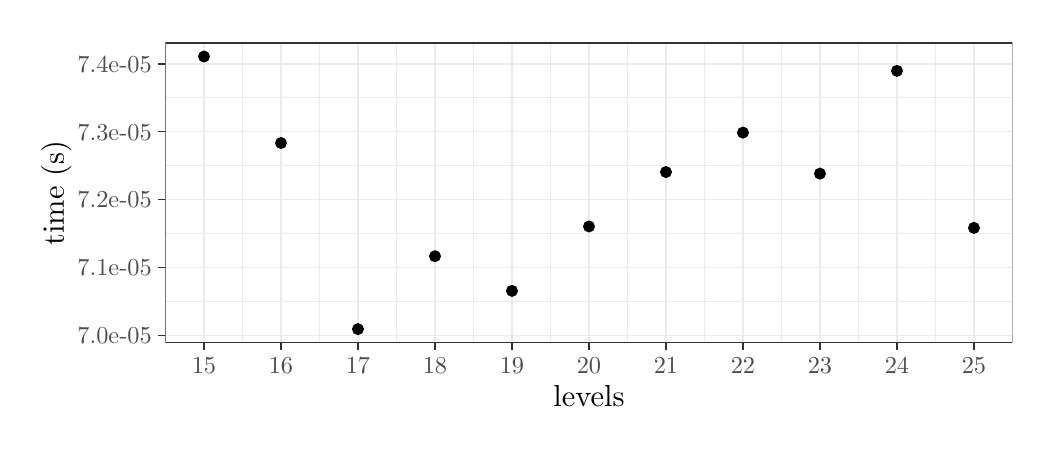
\begin{tikzpicture}[x=1pt,y=1pt]
\definecolor{fillColor}{RGB}{255,255,255}
\path[use as bounding box,fill=fillColor,fill opacity=0.00] (0,0) rectangle (361.35,144.54);
\begin{scope}
\path[clip] (  0.00,  0.00) rectangle (361.35,144.54);
\definecolor{drawColor}{RGB}{255,255,255}
\definecolor{fillColor}{RGB}{255,255,255}

\path[draw=drawColor,line width= 0.6pt,line join=round,line cap=round,fill=fillColor] (  0.00,  0.00) rectangle (361.35,144.54);
\end{scope}
\begin{scope}
\path[clip] ( 49.80, 30.69) rectangle (355.85,139.04);
\definecolor{fillColor}{RGB}{255,255,255}

\path[fill=fillColor] ( 49.80, 30.69) rectangle (355.85,139.04);
\definecolor{drawColor}{gray}{0.92}

\path[draw=drawColor,line width= 0.3pt,line join=round] ( 49.80, 45.59) --
	(355.85, 45.59);

\path[draw=drawColor,line width= 0.3pt,line join=round] ( 49.80, 70.14) --
	(355.85, 70.14);

\path[draw=drawColor,line width= 0.3pt,line join=round] ( 49.80, 94.69) --
	(355.85, 94.69);

\path[draw=drawColor,line width= 0.3pt,line join=round] ( 49.80,119.24) --
	(355.85,119.24);

\path[draw=drawColor,line width= 0.3pt,line join=round] ( 49.80, 30.69) --
	( 49.80,139.04);

\path[draw=drawColor,line width= 0.3pt,line join=round] ( 77.62, 30.69) --
	( 77.62,139.04);

\path[draw=drawColor,line width= 0.3pt,line join=round] (105.44, 30.69) --
	(105.44,139.04);

\path[draw=drawColor,line width= 0.3pt,line join=round] (133.27, 30.69) --
	(133.27,139.04);

\path[draw=drawColor,line width= 0.3pt,line join=round] (161.09, 30.69) --
	(161.09,139.04);

\path[draw=drawColor,line width= 0.3pt,line join=round] (188.91, 30.69) --
	(188.91,139.04);

\path[draw=drawColor,line width= 0.3pt,line join=round] (216.73, 30.69) --
	(216.73,139.04);

\path[draw=drawColor,line width= 0.3pt,line join=round] (244.56, 30.69) --
	(244.56,139.04);

\path[draw=drawColor,line width= 0.3pt,line join=round] (272.38, 30.69) --
	(272.38,139.04);

\path[draw=drawColor,line width= 0.3pt,line join=round] (300.20, 30.69) --
	(300.20,139.04);

\path[draw=drawColor,line width= 0.3pt,line join=round] (328.03, 30.69) --
	(328.03,139.04);

\path[draw=drawColor,line width= 0.3pt,line join=round] (355.85, 30.69) --
	(355.85,139.04);

\path[draw=drawColor,line width= 0.6pt,line join=round] ( 49.80, 33.32) --
	(355.85, 33.32);

\path[draw=drawColor,line width= 0.6pt,line join=round] ( 49.80, 57.87) --
	(355.85, 57.87);

\path[draw=drawColor,line width= 0.6pt,line join=round] ( 49.80, 82.42) --
	(355.85, 82.42);

\path[draw=drawColor,line width= 0.6pt,line join=round] ( 49.80,106.96) --
	(355.85,106.96);

\path[draw=drawColor,line width= 0.6pt,line join=round] ( 49.80,131.51) --
	(355.85,131.51);

\path[draw=drawColor,line width= 0.6pt,line join=round] ( 63.71, 30.69) --
	( 63.71,139.04);

\path[draw=drawColor,line width= 0.6pt,line join=round] ( 91.53, 30.69) --
	( 91.53,139.04);

\path[draw=drawColor,line width= 0.6pt,line join=round] (119.35, 30.69) --
	(119.35,139.04);

\path[draw=drawColor,line width= 0.6pt,line join=round] (147.18, 30.69) --
	(147.18,139.04);

\path[draw=drawColor,line width= 0.6pt,line join=round] (175.00, 30.69) --
	(175.00,139.04);

\path[draw=drawColor,line width= 0.6pt,line join=round] (202.82, 30.69) --
	(202.82,139.04);

\path[draw=drawColor,line width= 0.6pt,line join=round] (230.65, 30.69) --
	(230.65,139.04);

\path[draw=drawColor,line width= 0.6pt,line join=round] (258.47, 30.69) --
	(258.47,139.04);

\path[draw=drawColor,line width= 0.6pt,line join=round] (286.29, 30.69) --
	(286.29,139.04);

\path[draw=drawColor,line width= 0.6pt,line join=round] (314.12, 30.69) --
	(314.12,139.04);

\path[draw=drawColor,line width= 0.6pt,line join=round] (341.94, 30.69) --
	(341.94,139.04);
\definecolor{drawColor}{RGB}{0,0,0}
\definecolor{fillColor}{RGB}{0,0,0}

\path[draw=drawColor,line width= 0.4pt,line join=round,line cap=round,fill=fillColor] ( 63.71,134.11) circle (  1.96);

\path[draw=drawColor,line width= 0.4pt,line join=round,line cap=round,fill=fillColor] ( 91.53,102.87) circle (  1.96);

\path[draw=drawColor,line width= 0.4pt,line join=round,line cap=round,fill=fillColor] (119.35, 35.61) circle (  1.96);

\path[draw=drawColor,line width= 0.4pt,line join=round,line cap=round,fill=fillColor] (147.18, 61.96) circle (  1.96);

\path[draw=drawColor,line width= 0.4pt,line join=round,line cap=round,fill=fillColor] (175.00, 49.43) circle (  1.96);

\path[draw=drawColor,line width= 0.4pt,line join=round,line cap=round,fill=fillColor] (202.82, 72.71) circle (  1.96);

\path[draw=drawColor,line width= 0.4pt,line join=round,line cap=round,fill=fillColor] (230.65, 92.37) circle (  1.96);

\path[draw=drawColor,line width= 0.4pt,line join=round,line cap=round,fill=fillColor] (258.47,106.62) circle (  1.96);

\path[draw=drawColor,line width= 0.4pt,line join=round,line cap=round,fill=fillColor] (286.29, 91.80) circle (  1.96);

\path[draw=drawColor,line width= 0.4pt,line join=round,line cap=round,fill=fillColor] (314.12,128.93) circle (  1.96);

\path[draw=drawColor,line width= 0.4pt,line join=round,line cap=round,fill=fillColor] (341.94, 72.19) circle (  1.96);
\definecolor{drawColor}{gray}{0.20}

\path[draw=drawColor,line width= 0.6pt,line join=round,line cap=round] ( 49.80, 30.69) rectangle (355.85,139.04);
\end{scope}
\begin{scope}
\path[clip] (  0.00,  0.00) rectangle (361.35,144.54);
\definecolor{drawColor}{gray}{0.30}

\node[text=drawColor,anchor=base east,inner sep=0pt, outer sep=0pt, scale=  0.88] at ( 44.85, 30.29) {7.0e-05};

\node[text=drawColor,anchor=base east,inner sep=0pt, outer sep=0pt, scale=  0.88] at ( 44.85, 54.84) {7.1e-05};

\node[text=drawColor,anchor=base east,inner sep=0pt, outer sep=0pt, scale=  0.88] at ( 44.85, 79.39) {7.2e-05};

\node[text=drawColor,anchor=base east,inner sep=0pt, outer sep=0pt, scale=  0.88] at ( 44.85,103.93) {7.3e-05};

\node[text=drawColor,anchor=base east,inner sep=0pt, outer sep=0pt, scale=  0.88] at ( 44.85,128.48) {7.4e-05};
\end{scope}
\begin{scope}
\path[clip] (  0.00,  0.00) rectangle (361.35,144.54);
\definecolor{drawColor}{gray}{0.20}

\path[draw=drawColor,line width= 0.6pt,line join=round] ( 47.05, 33.32) --
	( 49.80, 33.32);

\path[draw=drawColor,line width= 0.6pt,line join=round] ( 47.05, 57.87) --
	( 49.80, 57.87);

\path[draw=drawColor,line width= 0.6pt,line join=round] ( 47.05, 82.42) --
	( 49.80, 82.42);

\path[draw=drawColor,line width= 0.6pt,line join=round] ( 47.05,106.96) --
	( 49.80,106.96);

\path[draw=drawColor,line width= 0.6pt,line join=round] ( 47.05,131.51) --
	( 49.80,131.51);
\end{scope}
\begin{scope}
\path[clip] (  0.00,  0.00) rectangle (361.35,144.54);
\definecolor{drawColor}{gray}{0.20}

\path[draw=drawColor,line width= 0.6pt,line join=round] ( 63.71, 27.94) --
	( 63.71, 30.69);

\path[draw=drawColor,line width= 0.6pt,line join=round] ( 91.53, 27.94) --
	( 91.53, 30.69);

\path[draw=drawColor,line width= 0.6pt,line join=round] (119.35, 27.94) --
	(119.35, 30.69);

\path[draw=drawColor,line width= 0.6pt,line join=round] (147.18, 27.94) --
	(147.18, 30.69);

\path[draw=drawColor,line width= 0.6pt,line join=round] (175.00, 27.94) --
	(175.00, 30.69);

\path[draw=drawColor,line width= 0.6pt,line join=round] (202.82, 27.94) --
	(202.82, 30.69);

\path[draw=drawColor,line width= 0.6pt,line join=round] (230.65, 27.94) --
	(230.65, 30.69);

\path[draw=drawColor,line width= 0.6pt,line join=round] (258.47, 27.94) --
	(258.47, 30.69);

\path[draw=drawColor,line width= 0.6pt,line join=round] (286.29, 27.94) --
	(286.29, 30.69);

\path[draw=drawColor,line width= 0.6pt,line join=round] (314.12, 27.94) --
	(314.12, 30.69);

\path[draw=drawColor,line width= 0.6pt,line join=round] (341.94, 27.94) --
	(341.94, 30.69);
\end{scope}
\begin{scope}
\path[clip] (  0.00,  0.00) rectangle (361.35,144.54);
\definecolor{drawColor}{gray}{0.30}

\node[text=drawColor,anchor=base,inner sep=0pt, outer sep=0pt, scale=  0.88] at ( 63.71, 19.68) {15};

\node[text=drawColor,anchor=base,inner sep=0pt, outer sep=0pt, scale=  0.88] at ( 91.53, 19.68) {16};

\node[text=drawColor,anchor=base,inner sep=0pt, outer sep=0pt, scale=  0.88] at (119.35, 19.68) {17};

\node[text=drawColor,anchor=base,inner sep=0pt, outer sep=0pt, scale=  0.88] at (147.18, 19.68) {18};

\node[text=drawColor,anchor=base,inner sep=0pt, outer sep=0pt, scale=  0.88] at (175.00, 19.68) {19};

\node[text=drawColor,anchor=base,inner sep=0pt, outer sep=0pt, scale=  0.88] at (202.82, 19.68) {20};

\node[text=drawColor,anchor=base,inner sep=0pt, outer sep=0pt, scale=  0.88] at (230.65, 19.68) {21};

\node[text=drawColor,anchor=base,inner sep=0pt, outer sep=0pt, scale=  0.88] at (258.47, 19.68) {22};

\node[text=drawColor,anchor=base,inner sep=0pt, outer sep=0pt, scale=  0.88] at (286.29, 19.68) {23};

\node[text=drawColor,anchor=base,inner sep=0pt, outer sep=0pt, scale=  0.88] at (314.12, 19.68) {24};

\node[text=drawColor,anchor=base,inner sep=0pt, outer sep=0pt, scale=  0.88] at (341.94, 19.68) {25};
\end{scope}
\begin{scope}
\path[clip] (  0.00,  0.00) rectangle (361.35,144.54);
\definecolor{drawColor}{RGB}{0,0,0}

\node[text=drawColor,anchor=base,inner sep=0pt, outer sep=0pt, scale=  1.10] at (202.82,  7.64) {levels};
\end{scope}
\begin{scope}
\path[clip] (  0.00,  0.00) rectangle (361.35,144.54);
\definecolor{drawColor}{RGB}{0,0,0}

\node[text=drawColor,rotate= 90.00,anchor=base,inner sep=0pt, outer sep=0pt, scale=  1.10] at ( 13.08, 84.86) {time (s)};
\end{scope}
\end{tikzpicture}


Sorprendentemente il numero ottimale di livelli non coincide esattamente con $ln(n)$

\chapter*{Esercizio 3}
\section{Minimum Heap}

\chapter*{Esercizio 4}
\section{Graph}

\end{document}